\documentclass{article}

\usepackage[utf8]{inputenc}
\usepackage[T1]{fontenc}
\usepackage[catalan]{babel}
\usepackage{cmbright}
\usepackage{lmodern}
\usepackage{geometry}
\usepackage{tikz}
\usepackage{hyperref}
\usepackage[bf,sf,pagestyles]{titlesec}
\usepackage{titling}
\usepackage[runin]{abstract}
\usepackage[font={footnotesize, sf}, labelfont=bf]{caption} 
\usepackage{siunitx}
\usepackage{graphicx}
\usepackage{float}
\usepackage{booktabs}
\usepackage{listings}
\usepackage{textcomp}
\usepackage{amsmath,amssymb}
\usepackage[sort]{cleveref}
\usepackage{enumitem}
\usepackage{mathtools}
\usepackage[sorting=none,citestyle=numeric]{biblatex}
\usepackage{subfig}
\usepackage{multirow}
\renewcommand{\familydefault}{\rmdefault}
\renewcommand{\sfdefault}{cmbr}
\renewcommand{\ttdefault}{cmtl}

\addbibresource{fonts.bib} 
\defbibheading{biblio}{\section*{#1}}

\geometry{
	a4paper,
	right = 2.5cm,
	left = 2.5cm,
	bottom = 3cm,
	top = 3cm
}

\hypersetup{
	colorlinks,
	linkcolor = {red!50!blue},
	citecolor = {red!50!blue},
	linktoc = page
}

\numberwithin{table}{section}
\numberwithin{figure}{section}
\numberwithin{equation}{section}

\graphicspath{{./figs/}}

% Unitats
\sisetup{
	inter-unit-product = \ensuremath{ \, },
	allow-number-unit-breaks = true,
	math-celsius = {}^{\circ}\kern-\scriptspace C,
	detect-family = true,
	detect-shape = true,
	list-final-separator = { y },
	list-pair-separator = { y },
	list-units = single,
	separate-uncertainty = true
}

\lstdefinestyle{customc}{
  belowcaptionskip=1\baselineskip,
	backgroundcolor = \color{gray!20!white},
  breaklines=true,
	breakatwhitespace = true,
	postbreak = \textrightarrow\,,
  xleftmargin=\parindent,
	frame = l,
  language=C,
  showstringspaces=false,
  basicstyle=\small\ttfamily,
  keywordstyle=\bfseries\color{green!40!black},
  commentstyle=\sffamily\itshape\color{purple!40!black},
  identifierstyle=\color{blue},
  stringstyle=\color{orange},
	numbers = left, 
	numberstyle = \tiny\ttfamily,
}
\lstset{texcl=true,style=customc}
\renewcommand{\lstlistingname}{Programa}

\newpagestyle{pagina}{
	\headrule
	\sethead*{\sffamily \bfseries Práctica 4}{}{\theauthor}
	\footrule
	\setfoot*{}{}{\sffamily \thepage}
}
\pagestyle{pagina}

\title{\sffamily \bfseries Modelització i anàlisi financera de l'empresa Caterpillar \vspace{1em} \hrule}
\author{\sffamily Andreu Arderiu, Arnau Mas}
\date{\sffamily 14 de juny de 2019}

\begin{document}

\begin{titlepage}
	\clearpage
	\thispagestyle{empty}
	\maketitle	

	\renewcommand{\abstractname}{\bfseries \sffamily Resum:}
	\begin{abstract}
		Abstract en català
	\end{abstract}

	\renewcommand{\abstractname}{\bfseries \sffamily Abstract:}
	\begin{abstract}
		Abstract en anglès
	\end{abstract}

	\begin{figure}[b]
		\thispagestyle{empty}
		\center 
\includegraphics[scale = 0.3]{uab}
	\end{figure}
\end{titlepage}

\begin{figure}[H]
	\centering \small \sffamily
	
\includegraphics[width=0.4\textwidth]{cat-logo}
	\caption{Logotip de Caterpillar}
\end{figure}
\textbf{En aquest estudi de l'empresa Caterpillar amb \textit{Symbol} bursàtil a la borsa de Nova York CAT, ens centrarem en els anys $2015-2018$. Mitjançant la comanda $getSymbols$ de R prenem un total de $1005$ dades corresponents als preus de tancament diari. A partir d'aquestes dades, podem calcular els estadístics bàsics de les rendibilitats, és a dir, els increments dels logaritmes dels preus. Trobem així una mitjana anual de $\hat{\mu}_a=0.07786318$, una desviació estàndard anual de $\hat{\sigma}_a=0.267607$, i finalment una curtosi diària de $\hat{ku}_d=2.806694$. }



\section{Context}
Caterpillar Inc. (NYSE: CAT) és una empresa multinacional de maquinària industrial i de construcció amb seu a Illinois. Actualment és l'empresa líder en l'àmbit de la maquinària de construcció i industrial \cite{cat} i es troba en la posició 65 al rànquing \emph{Fortune 500} i en la posició 238 del rànquing \emph{Fortune Global 500} de l'any 2019 \cite{fortune,global}. El preu actual de l'acció de Caterpillar és d'uns \$127. Actualment té \num{104000} treballadors. 

Caterpillar va néixer l'any 1925 de la fusió de les empreses Holt Manufacturing Company i C. L. Best Tractor Co. El fundador de la primera, Benjamin Holt, va patentar un dels primers vehicles que funcionaven amb tracció per eruga (d'aquí el nom Caterpillar), un sistema de tracció que consisteix en una sèrie de plaques rígides unides per una cinta que gira al voltant de les rodes del vehicle. Amb aquest sistema, la superfície de contacte del vehicle amb el sòl s'incrementa de manera que s'exerceix menys pressió i és possible circular per a terrenys més complicats. Originalment, els vehicles de Holt es feien servir a l'oest americà, on la combinació del terreny àrid i irregular del desert californià i la manca d'infraestructura dificultaven les tasques agràries i de transport. Molt aviat, però, l'empresa va desenvolupar vehicles militars durant la Primera Guerra Mundial, que van ser uns dels precursors del tanc. Durant el període d'entreguerra i sobretot després de la Segona Guerra Mundial, Caterpillar va evolucionar cap a l'àmbit de la construcció, primer al mercat americà i després a escala global, sobretot als països en desenvolupament. 

\begin{figure}[htb]
	\centering \sffamily \small
	% Created by tikzDevice version 0.12 on 2019-06-13 13:45:03
% !TEX encoding = UTF-8 Unicode
\begin{tikzpicture}[x=1pt,y=1pt]
\definecolor{fillColor}{RGB}{255,255,255}
\path[use as bounding box,fill=fillColor,fill opacity=0.00] (0,0) rectangle (433.62,122.86);
\begin{scope}
\path[clip] ( 21.60, 32.40) rectangle (412.02,122.86);
\definecolor{drawColor}{RGB}{169,169,169}

\path[draw=drawColor,line width= 0.4pt,line join=round,line cap=round] ( 36.06, 35.75) -- ( 36.06,107.54);

\path[draw=drawColor,line width= 0.4pt,line join=round,line cap=round] ( 55.08, 35.75) -- ( 55.08,107.54);

\path[draw=drawColor,line width= 0.4pt,line join=round,line cap=round] ( 74.09, 35.75) -- ( 74.09,107.54);

\path[draw=drawColor,line width= 0.4pt,line join=round,line cap=round] ( 93.11, 35.75) -- ( 93.11,107.54);

\path[draw=drawColor,line width= 0.4pt,line join=round,line cap=round] (112.12, 35.75) -- (112.12,107.54);

\path[draw=drawColor,line width= 0.4pt,line join=round,line cap=round] (131.24, 35.75) -- (131.24,107.54);

\path[draw=drawColor,line width= 0.4pt,line join=round,line cap=round] (150.26, 35.75) -- (150.26,107.54);

\path[draw=drawColor,line width= 0.4pt,line join=round,line cap=round] (169.27, 35.75) -- (169.27,107.54);

\path[draw=drawColor,line width= 0.4pt,line join=round,line cap=round] (188.23, 35.75) -- (188.23,107.54);

\path[draw=drawColor,line width= 0.4pt,line join=round,line cap=round] (207.30, 35.75) -- (207.30,107.54);

\path[draw=drawColor,line width= 0.4pt,line join=round,line cap=round] (226.42, 35.75) -- (226.42,107.54);

\path[draw=drawColor,line width= 0.4pt,line join=round,line cap=round] (245.39, 35.75) -- (245.39,107.54);

\path[draw=drawColor,line width= 0.4pt,line join=round,line cap=round] (264.40, 35.75) -- (264.40,107.54);

\path[draw=drawColor,line width= 0.4pt,line join=round,line cap=round] (283.42, 35.75) -- (283.42,107.54);

\path[draw=drawColor,line width= 0.4pt,line join=round,line cap=round] (302.43, 35.75) -- (302.43,107.54);

\path[draw=drawColor,line width= 0.4pt,line join=round,line cap=round] (321.45, 35.75) -- (321.45,107.54);

\path[draw=drawColor,line width= 0.4pt,line join=round,line cap=round] (340.57, 35.75) -- (340.57,107.54);

\path[draw=drawColor,line width= 0.4pt,line join=round,line cap=round] (359.58, 35.75) -- (359.58,107.54);

\path[draw=drawColor,line width= 0.4pt,line join=round,line cap=round] (378.54, 35.75) -- (378.54,107.54);

\path[draw=drawColor,line width= 0.4pt,line join=round,line cap=round] (397.56, 35.75) -- (397.56,107.54);

\path[draw=drawColor,line width= 0.4pt,line join=round,line cap=round] (397.56, 35.75) -- (397.56,107.54);
\end{scope}
\begin{scope}
\path[clip] (  0.00,  0.00) rectangle (433.62,122.86);
\definecolor{drawColor}{gray}{0.96}

\path[draw=drawColor,line width= 0.4pt,line join=round,line cap=round] ( 36.06, 32.40) -- (397.56, 32.40);

\path[draw=drawColor,line width= 0.4pt,line join=round,line cap=round] ( 36.06, 32.40) -- ( 36.06, 35.64);

\path[draw=drawColor,line width= 0.4pt,line join=round,line cap=round] ( 55.08, 32.40) -- ( 55.08, 35.64);

\path[draw=drawColor,line width= 0.4pt,line join=round,line cap=round] ( 74.09, 32.40) -- ( 74.09, 35.64);

\path[draw=drawColor,line width= 0.4pt,line join=round,line cap=round] ( 93.11, 32.40) -- ( 93.11, 35.64);

\path[draw=drawColor,line width= 0.4pt,line join=round,line cap=round] (112.12, 32.40) -- (112.12, 35.64);

\path[draw=drawColor,line width= 0.4pt,line join=round,line cap=round] (131.24, 32.40) -- (131.24, 35.64);

\path[draw=drawColor,line width= 0.4pt,line join=round,line cap=round] (150.26, 32.40) -- (150.26, 35.64);

\path[draw=drawColor,line width= 0.4pt,line join=round,line cap=round] (169.27, 32.40) -- (169.27, 35.64);

\path[draw=drawColor,line width= 0.4pt,line join=round,line cap=round] (188.23, 32.40) -- (188.23, 35.64);

\path[draw=drawColor,line width= 0.4pt,line join=round,line cap=round] (207.30, 32.40) -- (207.30, 35.64);

\path[draw=drawColor,line width= 0.4pt,line join=round,line cap=round] (226.42, 32.40) -- (226.42, 35.64);

\path[draw=drawColor,line width= 0.4pt,line join=round,line cap=round] (245.39, 32.40) -- (245.39, 35.64);

\path[draw=drawColor,line width= 0.4pt,line join=round,line cap=round] (264.40, 32.40) -- (264.40, 35.64);

\path[draw=drawColor,line width= 0.4pt,line join=round,line cap=round] (283.42, 32.40) -- (283.42, 35.64);

\path[draw=drawColor,line width= 0.4pt,line join=round,line cap=round] (302.43, 32.40) -- (302.43, 35.64);

\path[draw=drawColor,line width= 0.4pt,line join=round,line cap=round] (321.45, 32.40) -- (321.45, 35.64);

\path[draw=drawColor,line width= 0.4pt,line join=round,line cap=round] (340.57, 32.40) -- (340.57, 35.64);

\path[draw=drawColor,line width= 0.4pt,line join=round,line cap=round] (359.58, 32.40) -- (359.58, 35.64);

\path[draw=drawColor,line width= 0.4pt,line join=round,line cap=round] (378.54, 32.40) -- (378.54, 35.64);

\path[draw=drawColor,line width= 0.4pt,line join=round,line cap=round] (397.56, 32.40) -- (397.56, 35.64);
\end{scope}
\begin{scope}
\path[clip] (  0.00,  0.00) rectangle (433.62,122.86);
\definecolor{drawColor}{gray}{0.20}

\path[draw=drawColor,line width= 0.4pt,line join=round,line cap=round] ( 36.06, 32.40) -- (397.56, 32.40);

\path[draw=drawColor,line width= 0.6pt,line join=round,line cap=round] ( 36.06, 32.40) -- ( 36.06, 28.08);

\path[draw=drawColor,line width= 0.6pt,line join=round,line cap=round] ( 55.08, 32.40) -- ( 55.08, 28.08);

\path[draw=drawColor,line width= 0.6pt,line join=round,line cap=round] ( 74.09, 32.40) -- ( 74.09, 28.08);

\path[draw=drawColor,line width= 0.6pt,line join=round,line cap=round] ( 93.11, 32.40) -- ( 93.11, 28.08);

\path[draw=drawColor,line width= 0.6pt,line join=round,line cap=round] (112.12, 32.40) -- (112.12, 28.08);

\path[draw=drawColor,line width= 0.6pt,line join=round,line cap=round] (131.24, 32.40) -- (131.24, 28.08);

\path[draw=drawColor,line width= 0.6pt,line join=round,line cap=round] (150.26, 32.40) -- (150.26, 28.08);

\path[draw=drawColor,line width= 0.6pt,line join=round,line cap=round] (169.27, 32.40) -- (169.27, 28.08);

\path[draw=drawColor,line width= 0.6pt,line join=round,line cap=round] (188.23, 32.40) -- (188.23, 28.08);

\path[draw=drawColor,line width= 0.6pt,line join=round,line cap=round] (207.30, 32.40) -- (207.30, 28.08);

\path[draw=drawColor,line width= 0.6pt,line join=round,line cap=round] (226.42, 32.40) -- (226.42, 28.08);

\path[draw=drawColor,line width= 0.6pt,line join=round,line cap=round] (245.39, 32.40) -- (245.39, 28.08);

\path[draw=drawColor,line width= 0.6pt,line join=round,line cap=round] (264.40, 32.40) -- (264.40, 28.08);

\path[draw=drawColor,line width= 0.6pt,line join=round,line cap=round] (283.42, 32.40) -- (283.42, 28.08);

\path[draw=drawColor,line width= 0.6pt,line join=round,line cap=round] (302.43, 32.40) -- (302.43, 28.08);

\path[draw=drawColor,line width= 0.6pt,line join=round,line cap=round] (321.45, 32.40) -- (321.45, 28.08);

\path[draw=drawColor,line width= 0.6pt,line join=round,line cap=round] (340.57, 32.40) -- (340.57, 28.08);

\path[draw=drawColor,line width= 0.6pt,line join=round,line cap=round] (359.58, 32.40) -- (359.58, 28.08);

\path[draw=drawColor,line width= 0.6pt,line join=round,line cap=round] (378.54, 32.40) -- (378.54, 28.08);

\path[draw=drawColor,line width= 0.6pt,line join=round,line cap=round] (397.56, 32.40) -- (397.56, 28.08);

\path[draw=drawColor,line width= 0.6pt,line join=round,line cap=round] (397.56, 32.40) -- (397.56, 28.08);

\node[text=drawColor,anchor=base,inner sep=0pt, outer sep=0pt, scale=  0.81] at ( 36.06, 27.00) {};

\node[text=drawColor,anchor=base,inner sep=0pt, outer sep=0pt, scale=  0.81] at ( 36.06, 17.28) {Jan};

\node[text=drawColor,anchor=base,inner sep=0pt, outer sep=0pt, scale=  0.81] at ( 36.06,  7.56) {2000};

\node[text=drawColor,anchor=base,inner sep=0pt, outer sep=0pt, scale=  0.81] at ( 74.09, 27.00) {};

\node[text=drawColor,anchor=base,inner sep=0pt, outer sep=0pt, scale=  0.81] at ( 74.09, 17.28) {Jan};

\node[text=drawColor,anchor=base,inner sep=0pt, outer sep=0pt, scale=  0.81] at ( 74.09,  7.56) {2002};

\node[text=drawColor,anchor=base,inner sep=0pt, outer sep=0pt, scale=  0.81] at (112.12, 27.00) {};

\node[text=drawColor,anchor=base,inner sep=0pt, outer sep=0pt, scale=  0.81] at (112.12, 17.28) {Jan};

\node[text=drawColor,anchor=base,inner sep=0pt, outer sep=0pt, scale=  0.81] at (112.12,  7.56) {2004};

\node[text=drawColor,anchor=base,inner sep=0pt, outer sep=0pt, scale=  0.81] at (150.26, 27.00) {};

\node[text=drawColor,anchor=base,inner sep=0pt, outer sep=0pt, scale=  0.81] at (150.26, 17.28) {Jan};

\node[text=drawColor,anchor=base,inner sep=0pt, outer sep=0pt, scale=  0.81] at (150.26,  7.56) {2006};

\node[text=drawColor,anchor=base,inner sep=0pt, outer sep=0pt, scale=  0.81] at (188.23, 27.00) {};

\node[text=drawColor,anchor=base,inner sep=0pt, outer sep=0pt, scale=  0.81] at (188.23, 17.28) {Jan};

\node[text=drawColor,anchor=base,inner sep=0pt, outer sep=0pt, scale=  0.81] at (188.23,  7.56) {2008};

\node[text=drawColor,anchor=base,inner sep=0pt, outer sep=0pt, scale=  0.81] at (226.42, 27.00) {};

\node[text=drawColor,anchor=base,inner sep=0pt, outer sep=0pt, scale=  0.81] at (226.42, 17.28) {Jan};

\node[text=drawColor,anchor=base,inner sep=0pt, outer sep=0pt, scale=  0.81] at (226.42,  7.56) {2010};

\node[text=drawColor,anchor=base,inner sep=0pt, outer sep=0pt, scale=  0.81] at (264.40, 27.00) {};

\node[text=drawColor,anchor=base,inner sep=0pt, outer sep=0pt, scale=  0.81] at (264.40, 17.28) {Jan};

\node[text=drawColor,anchor=base,inner sep=0pt, outer sep=0pt, scale=  0.81] at (264.40,  7.56) {2012};

\node[text=drawColor,anchor=base,inner sep=0pt, outer sep=0pt, scale=  0.81] at (302.43, 27.00) {};

\node[text=drawColor,anchor=base,inner sep=0pt, outer sep=0pt, scale=  0.81] at (302.43, 17.28) {Jan};

\node[text=drawColor,anchor=base,inner sep=0pt, outer sep=0pt, scale=  0.81] at (302.43,  7.56) {2014};

\node[text=drawColor,anchor=base,inner sep=0pt, outer sep=0pt, scale=  0.81] at (340.57, 27.00) {};

\node[text=drawColor,anchor=base,inner sep=0pt, outer sep=0pt, scale=  0.81] at (340.57, 17.28) {Jan};

\node[text=drawColor,anchor=base,inner sep=0pt, outer sep=0pt, scale=  0.81] at (340.57,  7.56) {2016};

\node[text=drawColor,anchor=base,inner sep=0pt, outer sep=0pt, scale=  0.81] at (378.54, 27.00) {};

\node[text=drawColor,anchor=base,inner sep=0pt, outer sep=0pt, scale=  0.81] at (378.54, 17.28) {Jan};

\node[text=drawColor,anchor=base,inner sep=0pt, outer sep=0pt, scale=  0.81] at (378.54,  7.56) {2018};
\end{scope}
\begin{scope}
\path[clip] ( 21.60,107.54) rectangle (412.02,119.51);
\definecolor{drawColor}{gray}{0.20}

\node[text=drawColor,anchor=base west,inner sep=0pt, outer sep=0pt, scale=  0.99] at ( 36.06,111.25) {\bfseries Preus d'obertura entre 2000 i 2019};

\node[text=drawColor,anchor=base east,inner sep=0pt, outer sep=0pt, scale=  0.90] at (392.16,111.46) {2000-01-03 / 2019-01-02};
\end{scope}
\begin{scope}
\path[clip] ( 21.60, 35.75) rectangle (412.02,107.54);
\definecolor{drawColor}{RGB}{169,169,169}

\path[draw=drawColor,line width= 0.4pt,line join=round,line cap=round] ( 36.06, 44.78) -- (397.56, 44.78);

\path[draw=drawColor,line width= 0.4pt,line join=round,line cap=round] ( 36.06, 55.51) -- (397.56, 55.51);

\path[draw=drawColor,line width= 0.4pt,line join=round,line cap=round] ( 36.06, 66.23) -- (397.56, 66.23);

\path[draw=drawColor,line width= 0.4pt,line join=round,line cap=round] ( 36.06, 76.96) -- (397.56, 76.96);

\path[draw=drawColor,line width= 0.4pt,line join=round,line cap=round] ( 36.06, 87.68) -- (397.56, 87.68);

\path[draw=drawColor,line width= 0.4pt,line join=round,line cap=round] ( 36.06, 98.41) -- (397.56, 98.41);
\end{scope}
\begin{scope}
\path[clip] (  0.00,  0.00) rectangle (433.62,122.86);
\definecolor{drawColor}{gray}{0.20}

\node[text=drawColor,anchor=base east,inner sep=0pt, outer sep=0pt, scale=  0.81] at ( 25.26, 42.92) { 40};

\node[text=drawColor,anchor=base east,inner sep=0pt, outer sep=0pt, scale=  0.81] at ( 25.26, 53.65) { 60};

\node[text=drawColor,anchor=base east,inner sep=0pt, outer sep=0pt, scale=  0.81] at ( 25.26, 64.37) { 80};

\node[text=drawColor,anchor=base east,inner sep=0pt, outer sep=0pt, scale=  0.81] at ( 25.26, 75.10) {100};

\node[text=drawColor,anchor=base east,inner sep=0pt, outer sep=0pt, scale=  0.81] at ( 25.26, 85.82) {120};

\node[text=drawColor,anchor=base east,inner sep=0pt, outer sep=0pt, scale=  0.81] at ( 25.26, 96.55) {140};

\node[text=drawColor,anchor=base west,inner sep=0pt, outer sep=0pt, scale=  0.81] at (408.36, 42.92) { 40};

\node[text=drawColor,anchor=base west,inner sep=0pt, outer sep=0pt, scale=  0.81] at (408.36, 53.65) { 60};

\node[text=drawColor,anchor=base west,inner sep=0pt, outer sep=0pt, scale=  0.81] at (408.36, 64.37) { 80};

\node[text=drawColor,anchor=base west,inner sep=0pt, outer sep=0pt, scale=  0.81] at (408.36, 75.10) {100};

\node[text=drawColor,anchor=base west,inner sep=0pt, outer sep=0pt, scale=  0.81] at (408.36, 85.82) {120};

\node[text=drawColor,anchor=base west,inner sep=0pt, outer sep=0pt, scale=  0.81] at (408.36, 96.55) {140};
\end{scope}
\begin{scope}
\path[clip] ( 21.60, 35.75) rectangle (412.02,107.54);
\definecolor{drawColor}{RGB}{0,0,255}

\path[draw=drawColor,line width= 0.8pt,line join=round] ( 36.06, 36.37) --
	( 55.08, 35.75) --
	( 74.09, 37.18) --
	( 93.11, 36.14) --
	(112.12, 45.49) --
	(131.24, 48.82) --
	(150.26, 54.33) --
	(169.27, 56.13) --
	(188.23, 61.21) --
	(207.30, 48.49) --
	(226.42, 54.73) --
	(245.39, 73.82) --
	(264.40, 73.73) --
	(283.42, 73.47) --
	(302.43, 71.52) --
	(321.45, 72.60) --
	(340.57, 59.79) --
	(359.58, 73.73) --
	(378.54,107.54) --
	(397.56, 91.10);
\end{scope}
\end{tikzpicture}

	\caption{Preus d'obertura de Caterpillar entre els anys 2000 i 2019}
	\label{fig:tancament}
\end{figure}

A la \cref{fig:tancament} podem veure els preus d'obertura anuals de les accions de Caterpillar entre l'any 2000 i l'actualitat. La tendència és en general a l'alça, tot i que valen a remarcar diversos punts d'inflexió. És notable la forta caiguda de prop del \SI{35}{\percent} durant l'any 2008, naturalment deguda a la crisi financera del mateix any. Aquesta crisi va afectar fortament el sector de la construcció, que és una de les principals àrees de negoci de Caterpillar. Tanmateix, tal i com apunta \cite{recupera} l'empresa ja anticipava la recessió, i va prendre una sèrie de mesures que van alleujar l'impacte de la crisi. Això, juntament amb un canvi en la direcció, i un canvi d'estratègia enfocat a majors inversions a països amb un ràpid creixement econòmic com la Xina, Índia i Brasil, van fer que Caterpillar tingués una espectacular recuperació durant l'any 2010. Més endavant, durant l'any 2015 l'empresa va experimentar una altra davallada, de més del \SI{25}{\percent}, degut a la crisi del mercat financer xinès \cite{xina}, un dels principals clients de Caterpillar. Tot i així es va recuperar ràpidament durant 2016, iniciant l'any 2017 dos punts per sobre que el 2015, degut a un creixement del mercat, entre d'altres \cite{crush}. Per últim, l'increment dels aranzels sobre les importacions d'acer introduït pel govern de Trump han causat que el valor de Caterpillar hagi baixat prop d'un \SI{20}{\percent} durant l'any 2018 \cite{trump}.


\section{Estudi de les rendibilitats}



 



A la Figura \ref{fig:serie preus} veiem representat l'històric dels preus de tancament i rendibilitats diàries de Caterpillar al llarg dels últims 4 anys (2015-2018), en total 1005 i 1004 dades, respectivament. La mitjana i desviació estàndard mostrals per a la rendibilitat anual són $\hat{\mu}_a=0.07786318$ i $\hat{\sigma}_a=0.267607$, respectivament. El valor positiu obtingut per a $\hat{\mu}_a$, es pot resumir en que el creixement mitja del valor de les accions de Caterpillar durant aquest període ha estat positiu.\\
\begin{figure}[H]
	\centering \sffamily \small
	% Created by tikzDevice version 0.12 on 2019-06-12 19:23:20
% !TEX encoding = UTF-8 Unicode
\begin{tikzpicture}[x=1pt,y=1pt]
\definecolor{fillColor}{RGB}{255,255,255}
\path[use as bounding box,fill=fillColor,fill opacity=0.00] (0,0) rectangle (433.62,216.81);
\begin{scope}
\path[clip] ( 21.60, 32.40) rectangle (412.02,216.81);
\definecolor{drawColor}{RGB}{169,169,169}

\path[draw=drawColor,line width= 0.4pt,line join=round,line cap=round] ( 36.06, 84.16) -- ( 36.06,192.01);

\path[draw=drawColor,line width= 0.4pt,line join=round,line cap=round] ( 80.75, 84.16) -- ( 80.75,192.01);

\path[draw=drawColor,line width= 0.4pt,line join=round,line cap=round] (127.18, 84.16) -- (127.18,192.01);

\path[draw=drawColor,line width= 0.4pt,line join=round,line cap=round] (171.62, 84.16) -- (171.62,192.01);

\path[draw=drawColor,line width= 0.4pt,line join=round,line cap=round] (217.80, 84.16) -- (217.80,192.01);

\path[draw=drawColor,line width= 0.4pt,line join=round,line cap=round] (262.74, 84.16) -- (262.74,192.01);

\path[draw=drawColor,line width= 0.4pt,line join=round,line cap=round] (308.18, 84.16) -- (308.18,192.01);

\path[draw=drawColor,line width= 0.4pt,line join=round,line cap=round] (353.12, 84.16) -- (353.12,192.01);

\path[draw=drawColor,line width= 0.4pt,line join=round,line cap=round] (397.56, 84.16) -- (397.56,192.01);
\end{scope}
\begin{scope}
\path[clip] (  0.00,  0.00) rectangle (433.62,216.81);
\definecolor{drawColor}{gray}{0.20}

\path[draw=drawColor,line width= 0.4pt,line join=round,line cap=round] ( 36.06, 32.40) -- (397.56, 32.40);

\path[draw=drawColor,line width= 0.6pt,line join=round,line cap=round] ( 36.06, 32.40) -- ( 36.06, 28.08);

\path[draw=drawColor,line width= 0.6pt,line join=round,line cap=round] ( 80.75, 32.40) -- ( 80.75, 28.08);

\path[draw=drawColor,line width= 0.6pt,line join=round,line cap=round] (127.18, 32.40) -- (127.18, 28.08);

\path[draw=drawColor,line width= 0.6pt,line join=round,line cap=round] (171.62, 32.40) -- (171.62, 28.08);

\path[draw=drawColor,line width= 0.6pt,line join=round,line cap=round] (217.80, 32.40) -- (217.80, 28.08);

\path[draw=drawColor,line width= 0.6pt,line join=round,line cap=round] (262.74, 32.40) -- (262.74, 28.08);

\path[draw=drawColor,line width= 0.6pt,line join=round,line cap=round] (308.18, 32.40) -- (308.18, 28.08);

\path[draw=drawColor,line width= 0.6pt,line join=round,line cap=round] (353.12, 32.40) -- (353.12, 28.08);

\path[draw=drawColor,line width= 0.6pt,line join=round,line cap=round] (397.56, 32.40) -- (397.56, 28.08);

\node[text=drawColor,anchor=base,inner sep=0pt, outer sep=0pt, scale=  0.81] at ( 36.06, 17.28) {Jan 02};

\node[text=drawColor,anchor=base,inner sep=0pt, outer sep=0pt, scale=  0.81] at ( 36.06,  7.56) {2015};

\node[text=drawColor,anchor=base,inner sep=0pt, outer sep=0pt, scale=  0.81] at ( 80.75, 17.28) {Jul 01};

\node[text=drawColor,anchor=base,inner sep=0pt, outer sep=0pt, scale=  0.81] at ( 80.75,  7.56) {2015};

\node[text=drawColor,anchor=base,inner sep=0pt, outer sep=0pt, scale=  0.81] at (127.18, 17.28) {Jan 04};

\node[text=drawColor,anchor=base,inner sep=0pt, outer sep=0pt, scale=  0.81] at (127.18,  7.56) {2016};

\node[text=drawColor,anchor=base,inner sep=0pt, outer sep=0pt, scale=  0.81] at (171.62, 17.28) {Jul 01};

\node[text=drawColor,anchor=base,inner sep=0pt, outer sep=0pt, scale=  0.81] at (171.62,  7.56) {2016};

\node[text=drawColor,anchor=base,inner sep=0pt, outer sep=0pt, scale=  0.81] at (217.80, 17.28) {Jan 03};

\node[text=drawColor,anchor=base,inner sep=0pt, outer sep=0pt, scale=  0.81] at (217.80,  7.56) {2017};

\node[text=drawColor,anchor=base,inner sep=0pt, outer sep=0pt, scale=  0.81] at (262.74, 17.28) {Jul 03};

\node[text=drawColor,anchor=base,inner sep=0pt, outer sep=0pt, scale=  0.81] at (262.74,  7.56) {2017};

\node[text=drawColor,anchor=base,inner sep=0pt, outer sep=0pt, scale=  0.81] at (308.18, 17.28) {Jan 02};

\node[text=drawColor,anchor=base,inner sep=0pt, outer sep=0pt, scale=  0.81] at (308.18,  7.56) {2018};

\node[text=drawColor,anchor=base,inner sep=0pt, outer sep=0pt, scale=  0.81] at (353.12, 17.28) {Jul 02};

\node[text=drawColor,anchor=base,inner sep=0pt, outer sep=0pt, scale=  0.81] at (353.12,  7.56) {2018};

\node[text=drawColor,anchor=base,inner sep=0pt, outer sep=0pt, scale=  0.81] at (397.56, 17.28) {Dec 28};

\node[text=drawColor,anchor=base,inner sep=0pt, outer sep=0pt, scale=  0.81] at (397.56,  7.56) {2018};
\end{scope}
\begin{scope}
\path[clip] ( 21.60,192.01) rectangle (412.02,209.98);
\definecolor{drawColor}{gray}{0.20}

\node[text=drawColor,anchor=base west,inner sep=0pt, outer sep=0pt, scale=  0.99] at ( 36.06,198.72) {\bfseries Evolució del preu de tancament};

\node[text=drawColor,anchor=base east,inner sep=0pt, outer sep=0pt, scale=  0.90] at (392.16,198.93) {2015-01-02 / 2018-12-28};
\end{scope}
\begin{scope}
\path[clip] ( 21.60, 84.16) rectangle (412.02,192.01);
\definecolor{drawColor}{RGB}{169,169,169}

\path[draw=drawColor,line width= 0.4pt,line join=round,line cap=round] ( 36.06, 86.16) -- (397.56, 86.16);

\path[draw=drawColor,line width= 0.4pt,line join=round,line cap=round] ( 36.06,105.25) -- (397.56,105.25);

\path[draw=drawColor,line width= 0.4pt,line join=round,line cap=round] ( 36.06,124.34) -- (397.56,124.34);

\path[draw=drawColor,line width= 0.4pt,line join=round,line cap=round] ( 36.06,143.43) -- (397.56,143.43);

\path[draw=drawColor,line width= 0.4pt,line join=round,line cap=round] ( 36.06,162.52) -- (397.56,162.52);

\path[draw=drawColor,line width= 0.4pt,line join=round,line cap=round] ( 36.06,181.61) -- (397.56,181.61);
\end{scope}
\begin{scope}
\path[clip] (  0.00,  0.00) rectangle (433.62,216.81);
\definecolor{drawColor}{gray}{0.20}

\node[text=drawColor,anchor=base east,inner sep=0pt, outer sep=0pt, scale=  0.81] at ( 25.26, 84.30) { 60};

\node[text=drawColor,anchor=base east,inner sep=0pt, outer sep=0pt, scale=  0.81] at ( 25.26,103.39) { 80};

\node[text=drawColor,anchor=base east,inner sep=0pt, outer sep=0pt, scale=  0.81] at ( 25.26,122.48) {100};

\node[text=drawColor,anchor=base east,inner sep=0pt, outer sep=0pt, scale=  0.81] at ( 25.26,141.57) {120};

\node[text=drawColor,anchor=base east,inner sep=0pt, outer sep=0pt, scale=  0.81] at ( 25.26,160.66) {140};

\node[text=drawColor,anchor=base east,inner sep=0pt, outer sep=0pt, scale=  0.81] at ( 25.26,179.75) {160};

\node[text=drawColor,anchor=base west,inner sep=0pt, outer sep=0pt, scale=  0.81] at (408.36, 84.30) { 60};

\node[text=drawColor,anchor=base west,inner sep=0pt, outer sep=0pt, scale=  0.81] at (408.36,103.39) { 80};

\node[text=drawColor,anchor=base west,inner sep=0pt, outer sep=0pt, scale=  0.81] at (408.36,122.48) {100};

\node[text=drawColor,anchor=base west,inner sep=0pt, outer sep=0pt, scale=  0.81] at (408.36,141.57) {120};

\node[text=drawColor,anchor=base west,inner sep=0pt, outer sep=0pt, scale=  0.81] at (408.36,160.66) {140};

\node[text=drawColor,anchor=base west,inner sep=0pt, outer sep=0pt, scale=  0.81] at (408.36,179.75) {160};
\end{scope}
\begin{scope}
\path[clip] ( 21.60, 84.16) rectangle (412.02,192.01);
\definecolor{drawColor}{RGB}{0,0,0}

\path[draw=drawColor,line width= 0.8pt,line join=round] ( 36.06,116.59) --
	( 36.80,111.96) --
	( 37.05,111.43) --
	( 37.30,112.70) --
	( 37.55,113.56) --
	( 37.80,112.55) --
	( 38.54,111.83) --
	( 38.79,111.33) --
	( 39.04,111.04) --
	( 39.29,109.37) --
	( 39.54,108.93) --
	( 40.53,109.04) --
	( 40.78,110.38) --
	( 41.03,111.76) --
	( 41.27,110.60) --
	( 42.02,111.01) --
	( 42.27,105.11) --
	( 42.52,105.26) --
	( 42.76,105.25) --
	( 43.01,105.22) --
	( 43.76,106.05) --
	( 44.01,108.99) --
	( 44.25,107.11) --
	( 44.50,108.66) --
	( 44.75,108.31) --
	( 45.49,109.71) --
	( 45.74,108.97) --
	( 45.99,108.50) --
	( 46.24,108.62) --
	( 46.49,110.15) --
	( 47.48,110.38) --
	( 47.73,109.83) --
	( 47.98,108.40) --
	( 48.23,109.49) --
	( 48.97,108.58) --
	( 49.22,109.55) --
	( 49.47,110.17) --
	( 49.72,108.88) --
	( 49.96,108.02) --
	( 50.71,108.11) --
	( 50.96,107.96) --
	( 51.21,106.90) --
	( 51.45,106.69) --
	( 51.70,105.31) --
	( 52.45,106.02) --
	( 52.69,105.16) --
	( 52.94,104.96) --
	( 53.19,105.43) --
	( 53.44,104.51) --
	( 54.18,105.22) --
	( 54.43,103.77) --
	( 54.68,106.52) --
	( 54.93,105.34) --
	( 55.18,106.39) --
	( 55.92,106.29) --
	( 56.17,105.71) --
	( 56.42,105.12) --
	( 56.67,105.14) --
	( 56.92,104.93) --
	( 57.66,106.56) --
	( 57.91,105.28) --
	( 58.16,104.91) --
	( 58.41,105.48) --
	( 59.40,106.67) --
	( 59.65,105.77) --
	( 59.90,105.67) --
	( 60.14,105.90) --
	( 60.39,107.73) --
	( 61.14,107.29) --
	( 61.38,108.11) --
	( 61.63,110.17) --
	( 61.88,109.39) --
	( 62.13,108.38) --
	( 62.87,109.64) --
	( 63.12,108.99) --
	( 63.37,109.90) --
	( 63.62,109.82) --
	( 63.87,109.64) --
	( 64.61,110.34) --
	( 64.86,111.17) --
	( 65.11,112.41) --
	( 65.36,111.82) --
	( 65.61,112.28) --
	( 66.35,112.22) --
	( 66.60,111.93) --
	( 66.85,111.92) --
	( 67.10,111.39) --
	( 67.34,112.23) --
	( 68.09,113.62) --
	( 68.34,113.04) --
	( 68.59,113.31) --
	( 68.83,113.59) --
	( 69.08,113.30) --
	( 69.83,113.16) --
	( 70.07,112.16) --
	( 70.32,112.82) --
	( 70.57,114.16) --
	( 70.82,113.49) --
	( 71.81,112.73) --
	( 72.06,112.81) --
	( 72.31,110.99) --
	( 72.56,110.33) --
	( 73.30,110.53) --
	( 73.55,111.14) --
	( 73.80,111.20) --
	( 74.05,110.47) --
	( 74.30,111.02) --
	( 75.04,111.12) --
	( 75.29,111.67) --
	( 75.54,113.34) --
	( 75.79,113.05) --
	( 76.03,112.74) --
	( 76.78,112.06) --
	( 77.03,111.54) --
	( 77.27,112.17) --
	( 77.52,112.35) --
	( 77.77,112.43) --
	( 78.52,113.14) --
	( 78.76,113.32) --
	( 79.01,113.05) --
	( 79.26,111.66) --
	( 79.51,111.76) --
	( 80.25,110.31) --
	( 80.50,109.85) --
	( 80.75,109.02) --
	( 81.00,109.43) --
	( 81.99,108.26) --
	( 82.24,109.06) --
	( 82.49,107.42) --
	( 82.74,106.86) --
	( 82.99,107.30) --
	( 83.73,108.72) --
	( 83.98,109.51) --
	( 84.23,109.22) --
	( 84.48,108.84) --
	( 84.72,108.27) --
	( 85.47,107.40) --
	( 85.72,107.37) --
	( 85.96,105.02) --
	( 86.21,102.27) --
	( 86.46,101.53) --
	( 87.21,100.78) --
	( 87.45,103.13) --
	( 87.70,102.70) --
	( 87.95,103.67) --
	( 88.20,103.94) --
	( 88.94,102.63) --
	( 89.19,102.00) --
	( 89.44,102.27) --
	( 89.69,102.83) --
	( 89.94,102.66) --
	( 90.68,105.40) --
	( 90.93,103.38) --
	( 91.18,104.22) --
	( 91.43,103.11) --
	( 91.68,103.81) --
	( 92.42,103.86) --
	( 92.67,104.12) --
	( 92.92,102.78) --
	( 93.17,101.82) --
	( 93.41,100.48) --
	( 94.16, 98.40) --
	( 94.41, 97.67) --
	( 94.65, 99.40) --
	( 94.90,101.11) --
	( 95.15,101.38) --
	( 95.90,101.85) --
	( 96.14,100.38) --
	( 96.39,101.53) --
	( 96.64, 99.95) --
	( 96.89, 98.66) --
	( 97.88, 99.81) --
	( 98.13, 98.53) --
	( 98.38, 98.01) --
	( 98.63, 98.21) --
	( 99.37, 98.35) --
	( 99.62,100.08) --
	( 99.87,101.09) --
	(100.12, 99.58) --
	(100.37, 97.48) --
	(101.11, 97.77) --
	(101.36, 97.31) --
	(101.61, 95.90) --
	(101.85, 91.70) --
	(102.10, 90.91) --
	(102.85, 89.78) --
	(103.10, 90.27) --
	(103.34, 91.28) --
	(103.59, 90.35) --
	(103.84, 91.60) --
	(104.59, 94.92) --
	(104.83, 96.49) --
	(105.08, 96.07) --
	(105.33, 97.46) --
	(105.58, 96.95) --
	(106.32, 96.18) --
	(106.57, 95.87) --
	(106.82, 96.38) --
	(107.07, 96.50) --
	(107.32, 95.40) --
	(108.06, 95.01) --
	(108.31, 95.96) --
	(108.56, 95.39) --
	(108.81, 96.54) --
	(109.06, 97.37) --
	(109.80, 97.16) --
	(110.05, 96.08) --
	(110.30, 97.58) --
	(110.54, 97.58) --
	(110.79, 98.56) --
	(111.54, 99.85) --
	(111.79,100.24) --
	(112.03,100.05) --
	(112.28, 99.73) --
	(112.53, 99.37) --
	(113.28, 97.51) --
	(113.52, 98.02) --
	(113.77, 97.53) --
	(114.02, 94.43) --
	(114.27, 95.35) --
	(115.01, 96.08) --
	(115.26, 95.12) --
	(115.51, 96.01) --
	(115.76, 95.72) --
	(116.01, 96.79) --
	(116.75, 96.68) --
	(117.00, 97.04) --
	(117.25, 97.13) --
	(117.75, 96.87) --
	(118.49, 98.23) --
	(118.74, 97.19) --
	(118.99, 96.69) --
	(119.23, 95.36) --
	(119.48, 95.69) --
	(120.23, 94.14) --
	(120.48, 92.40) --
	(120.72, 91.80) --
	(120.97, 92.25) --
	(121.22, 91.34) --
	(121.97, 92.00) --
	(122.21, 92.60) --
	(122.46, 93.53) --
	(122.71, 90.84) --
	(122.96, 91.04) --
	(123.70, 91.16) --
	(123.95, 94.19) --
	(124.20, 95.60) --
	(124.45, 95.11) --
	(125.44, 94.35) --
	(125.69, 94.93) --
	(125.94, 94.45) --
	(126.19, 93.76) --
	(127.18, 93.79) --
	(127.43, 93.11) --
	(127.68, 92.10) --
	(127.92, 89.92) --
	(128.17, 89.30) --
	(128.92, 87.56) --
	(129.17, 87.69) --
	(129.41, 87.01) --
	(129.66, 88.33) --
	(129.91, 86.04) --
	(130.90, 85.23) --
	(131.15, 85.02) --
	(131.40, 85.86) --
	(131.65, 87.09) --
	(132.39, 84.16) --
	(132.64, 85.36) --
	(132.89, 84.56) --
	(133.14, 87.19) --
	(133.39, 88.30) --
	(134.13, 88.74) --
	(134.38, 86.80) --
	(134.63, 89.28) --
	(134.88, 91.85) --
	(135.12, 92.00) --
	(135.87, 90.53) --
	(136.12, 89.91) --
	(136.37, 88.20) --
	(136.61, 87.51) --
	(136.86, 89.17) --
	(137.86, 91.13) --
	(138.10, 93.09) --
	(138.35, 92.00) --
	(138.60, 91.33) --
	(139.35, 93.14) --
	(139.59, 91.68) --
	(139.84, 91.77) --
	(140.09, 92.33) --
	(140.34, 92.72) --
	(141.08, 93.51) --
	(141.33, 94.84) --
	(141.58, 95.11) --
	(141.83, 97.37) --
	(142.08, 98.42) --
	(142.82,100.26) --
	(143.07, 97.36) --
	(143.32, 97.49) --
	(143.57, 97.00) --
	(143.81, 98.38) --
	(144.56, 98.31) --
	(144.81, 98.03) --
	(145.06, 99.85) --
	(145.30,101.34) --
	(145.55,100.93) --
	(146.30,101.33) --
	(146.55,101.00) --
	(146.79, 99.22) --
	(147.04,100.75) --
	(148.04,100.78) --
	(148.28,101.44) --
	(148.53,101.92) --
	(148.78,101.95) --
	(149.03,102.19) --
	(149.77,101.16) --
	(150.02,100.71) --
	(150.27,100.69) --
	(150.52, 99.68) --
	(150.77, 99.86) --
	(151.51,100.12) --
	(151.76,101.53) --
	(152.01,104.42) --
	(152.26,104.34) --
	(152.50,104.46) --
	(153.25,104.53) --
	(153.50,105.62) --
	(153.75,105.00) --
	(153.99,103.97) --
	(154.24,103.65) --
	(154.99,102.19) --
	(155.24,103.01) --
	(155.48,103.99) --
	(155.73,103.10) --
	(155.98,103.07) --
	(156.73,103.19) --
	(156.97,101.78) --
	(157.22, 99.75) --
	(157.47, 98.37) --
	(157.72, 98.91) --
	(158.46, 96.45) --
	(158.71, 98.10) --
	(158.96, 98.02) --
	(159.21, 97.33) --
	(159.46, 95.77) --
	(160.20, 96.37) --
	(160.45, 96.71) --
	(160.70, 96.27) --
	(160.95, 95.16) --
	(161.19, 95.58) --
	(161.94, 96.09) --
	(162.19, 96.74) --
	(162.44, 98.16) --
	(162.68, 97.69) --
	(162.93, 97.58) --
	(163.93, 98.10) --
	(164.17, 97.87) --
	(164.42, 99.16) --
	(164.67,100.52) --
	(165.42,101.83) --
	(165.66,102.20) --
	(165.91,103.45) --
	(166.16,102.54) --
	(166.41,101.46) --
	(167.15,100.70) --
	(167.40,100.34) --
	(167.65,100.54) --
	(167.90,100.47) --
	(168.15,101.36) --
	(168.89,101.84) --
	(169.14,101.90) --
	(169.39,101.84) --
	(169.64,103.55) --
	(169.88, 98.60) --
	(170.63, 97.02) --
	(170.88, 98.11) --
	(171.13, 99.74) --
	(171.37,101.25) --
	(171.62,101.86) --
	(172.62, 99.89) --
	(172.86,100.31) --
	(173.11,100.52) --
	(173.36,102.74) --
	(174.11,103.15) --
	(174.35,105.06) --
	(174.60,104.95) --
	(174.85,105.31) --
	(175.10,105.92) --
	(175.84,105.08) --
	(176.09,105.00) --
	(176.34,104.95) --
	(176.59,105.26) --
	(176.84,104.66) --
	(177.58,104.00) --
	(177.83,107.87) --
	(178.08,109.16) --
	(178.33,108.04) --
	(178.57,107.88) --
	(179.32,107.11) --
	(179.57,106.43) --
	(179.82,107.19) --
	(180.06,106.94) --
	(180.31,107.69) --
	(181.06,108.53) --
	(181.31,107.95) --
	(181.55,107.78) --
	(181.80,108.34) --
	(182.05,108.11) --
	(182.80,109.21) --
	(183.04,109.34) --
	(183.29,109.46) --
	(183.54,108.48) --
	(183.79,108.92) --
	(184.53,108.68) --
	(184.78,109.08) --
	(185.03,108.26) --
	(185.28,107.96) --
	(185.53,107.79) --
	(186.27,108.21) --
	(186.52,107.62) --
	(186.77,107.11) --
	(187.02,106.63) --
	(187.26,106.86) --
	(188.26,107.24) --
	(188.51,108.80) --
	(188.75,108.63) --
	(189.00,106.00) --
	(189.75,107.08) --
	(190.00,105.47) --
	(190.24,106.22) --
	(190.49,107.19) --
	(190.74,107.21) --
	(191.49,107.04) --
	(191.73,106.87) --
	(191.98,108.56) --
	(192.23,108.59) --
	(192.48,107.58) --
	(193.22,107.51) --
	(193.47,108.00) --
	(193.72,111.54) --
	(193.97,112.38) --
	(194.22,113.62) --
	(194.96,113.15) --
	(195.21,112.42) --
	(195.46,114.24) --
	(195.71,114.12) --
	(195.95,113.33) --
	(196.70,113.10) --
	(196.95,112.38) --
	(197.20,112.48) --
	(197.44,111.90) --
	(197.69,112.57) --
	(198.44,112.21) --
	(198.69,112.14) --
	(198.93,112.89) --
	(199.18,111.58) --
	(199.43,111.29) --
	(200.18,110.97) --
	(200.42,109.53) --
	(200.67,109.19) --
	(200.92,108.12) --
	(201.17,108.95) --
	(201.91,108.55) --
	(202.16,107.39) --
	(202.41,106.31) --
	(202.66,106.46) --
	(202.91,107.45) --
	(203.65,108.83) --
	(203.90,109.72) --
	(204.15,115.94) --
	(204.40,118.09) --
	(204.64,117.67) --
	(205.39,118.78) --
	(205.64,119.03) --
	(205.89,117.99) --
	(206.13,117.45) --
	(206.38,117.03) --
	(207.13,117.56) --
	(207.38,118.25) --
	(207.62,120.69) --
	(208.12,120.34) --
	(208.86,119.47) --
	(209.11,118.65) --
	(209.36,120.10) --
	(209.61,120.75) --
	(209.86,119.70) --
	(210.60,119.04) --
	(210.85,119.78) --
	(211.10,121.79) --
	(211.35,120.78) --
	(211.60,120.07) --
	(212.34,119.64) --
	(212.59,120.54) --
	(212.84,118.36) --
	(213.09,119.12) --
	(213.33,117.26) --
	(214.08,117.38) --
	(214.33,118.94) --
	(214.58,118.44) --
	(214.82,118.73) --
	(215.07,118.92) --
	(216.07,119.14) --
	(216.31,117.80) --
	(216.56,117.94) --
	(216.81,117.41) --
	(217.80,118.60) --
	(218.05,118.20) --
	(218.30,117.66) --
	(218.55,117.70) --
	(219.29,117.06) --
	(219.54,118.45) --
	(219.79,119.23) --
	(220.04,118.60) --
	(220.29,119.07) --
	(221.28,118.20) --
	(221.53,117.97) --
	(221.78,118.02) --
	(222.02,119.17) --
	(222.77,119.05) --
	(223.02,120.75) --
	(223.27,122.57) --
	(223.51,121.69) --
	(223.76,123.38) --
	(224.51,121.28) --
	(224.76,120.20) --
	(225.00,119.67) --
	(225.25,118.39) --
	(225.50,117.93) --
	(226.24,117.53) --
	(226.49,117.95) --
	(226.74,117.57) --
	(226.99,118.57) --
	(227.24,120.82) --
	(227.98,122.91) --
	(228.23,122.52) --
	(228.48,123.40) --
	(228.73,122.68) --
	(228.98,123.24) --
	(229.97,122.53) --
	(230.22,122.62) --
	(230.47,120.09) --
	(230.71,120.03) --
	(231.46,121.90) --
	(231.71,121.15) --
	(231.96,122.98) --
	(232.20,118.96) --
	(232.45,119.68) --
	(233.20,120.20) --
	(233.44,120.46) --
	(233.69,117.88) --
	(233.94,116.12) --
	(234.19,117.00) --
	(234.93,117.31) --
	(235.18,116.57) --
	(235.43,118.00) --
	(235.68,117.52) --
	(235.93,117.57) --
	(236.67,119.95) --
	(236.92,117.11) --
	(237.17,117.11) --
	(237.42,116.92) --
	(237.67,116.85) --
	(238.41,116.24) --
	(238.66,117.61) --
	(238.91,117.52) --
	(239.16,117.87) --
	(239.40,117.43) --
	(240.15,116.96) --
	(240.40,118.74) --
	(240.65,118.84) --
	(240.89,120.35) --
	(241.14,120.06) --
	(241.89,121.61) --
	(242.13,121.57) --
	(242.38,119.43) --
	(242.63,117.75) --
	(243.62,118.75) --
	(243.87,118.99) --
	(244.12,118.11) --
	(244.37,119.24) --
	(244.62,118.92) --
	(245.36,121.30) --
	(245.61,128.56) --
	(245.86,128.79) --
	(246.11,126.90) --
	(246.36,126.50) --
	(247.10,126.25) --
	(247.35,125.78) --
	(247.60,125.81) --
	(247.85,123.76) --
	(248.09,124.00) --
	(248.84,123.74) --
	(249.09,123.66) --
	(249.34,124.68) --
	(249.58,125.29) --
	(249.83,125.02) --
	(250.58,126.65) --
	(250.82,126.57) --
	(251.07,124.47) --
	(251.32,124.55) --
	(251.57,126.66) --
	(252.31,126.53) --
	(252.56,127.81) --
	(252.81,128.11) --
	(253.06,129.13) --
	(253.31,129.74) --
	(254.30,129.56) --
	(254.55,129.52) --
	(254.80,129.73) --
	(255.05,130.02) --
	(255.79,129.30) --
	(256.04,128.68) --
	(256.29,127.69) --
	(256.54,129.12) --
	(256.78,129.99) --
	(257.53,130.13) --
	(257.78,129.83) --
	(258.02,128.84) --
	(258.27,130.45) --
	(258.52,131.59) --
	(259.27,131.49) --
	(259.51,131.06) --
	(259.76,127.65) --
	(260.01,128.01) --
	(260.26,128.26) --
	(261.00,128.40) --
	(261.25,128.09) --
	(261.50,130.50) --
	(261.75,129.72) --
	(262.00,131.46) --
	(262.74,130.99) --
	(263.24,131.49) --
	(263.49,130.55) --
	(263.74,130.95) --
	(264.48,131.82) --
	(264.73,132.21) --
	(264.98,132.89) --
	(265.23,132.42) --
	(265.47,132.71) --
	(266.22,132.78) --
	(266.47,131.09) --
	(266.71,131.83) --
	(266.96,131.33) --
	(267.21,130.63) --
	(267.96,132.15) --
	(268.20,138.22) --
	(268.45,137.25) --
	(268.70,138.06) --
	(268.95,137.80) --
	(269.69,137.66) --
	(269.94,136.84) --
	(270.19,136.83) --
	(270.44,137.28) --
	(270.69,138.04) --
	(271.43,138.38) --
	(271.68,138.09) --
	(271.93,138.03) --
	(272.18,136.89) --
	(272.43,136.61) --
	(273.17,137.43) --
	(273.42,137.37) --
	(273.67,137.82) --
	(273.92,136.88) --
	(274.16,137.63) --
	(274.91,137.32) --
	(275.16,139.44) --
	(275.40,138.42) --
	(275.65,138.45) --
	(275.90,138.99) --
	(276.65,138.72) --
	(276.89,139.62) --
	(277.14,141.09) --
	(277.39,141.03) --
	(277.64,141.79) --
	(278.63,141.81) --
	(278.88,140.55) --
	(279.13,141.30) --
	(279.38,141.35) --
	(280.12,142.35) --
	(280.37,144.33) --
	(280.62,143.08) --
	(280.87,143.89) --
	(281.12,144.74) --
	(281.86,147.09) --
	(282.11,147.96) --
	(282.36,148.06) --
	(282.60,148.00) --
	(282.85,147.66) --
	(283.60,147.55) --
	(283.85,147.74) --
	(284.09,147.75) --
	(284.34,148.42) --
	(284.59,147.93) --
	(285.34,147.94) --
	(285.58,148.69) --
	(285.83,149.86) --
	(286.08,149.54) --
	(286.33,150.05) --
	(287.07,150.00) --
	(287.32,151.25) --
	(287.57,151.64) --
	(287.82,152.97) --
	(288.07,153.65) --
	(288.81,154.38) --
	(289.06,153.49) --
	(289.31,154.21) --
	(289.56,154.46) --
	(289.81,154.27) --
	(290.55,154.58) --
	(290.80,160.84) --
	(291.05,159.50) --
	(291.29,159.60) --
	(291.54,160.43) --
	(292.29,159.17) --
	(292.54,158.51) --
	(292.78,158.98) --
	(293.03,159.15) --
	(293.28,159.30) --
	(294.03,160.34) --
	(294.27,161.39) --
	(294.52,159.93) --
	(294.77,158.07) --
	(295.02,159.16) --
	(295.76,159.21) --
	(296.01,160.17) --
	(296.26,156.89) --
	(296.51,159.05) --
	(296.76,158.83) --
	(297.50,159.57) --
	(297.75,160.23) --
	(298.00,160.62) --
	(298.50,160.03) --
	(299.24,159.84) --
	(299.49,161.56) --
	(299.74,160.67) --
	(299.98,163.62) --
	(300.23,163.97) --
	(300.98,163.95) --
	(301.23,162.65) --
	(301.47,162.85) --
	(301.72,165.28) --
	(301.97,166.21) --
	(302.72,166.12) --
	(302.96,165.79) --
	(303.21,170.70) --
	(303.46,168.52) --
	(303.71,168.91) --
	(304.45,171.85) --
	(304.70,172.93) --
	(304.95,174.47) --
	(305.20,176.50) --
	(305.45,177.55) --
	(306.44,178.21) --
	(306.69,179.24) --
	(306.94,180.10) --
	(307.19,179.30) --
	(308.18,178.79) --
	(308.43,179.02) --
	(308.67,181.08) --
	(308.92,183.48) --
	(309.67,187.37) --
	(309.92,187.75) --
	(310.16,187.21) --
	(310.41,190.39) --
	(310.66,191.44) --
	(311.65,190.50) --
	(311.90,189.73) --
	(312.15,190.04) --
	(312.40,191.55) --
	(313.14,192.01) --
	(313.39,190.61) --
	(313.64,189.57) --
	(313.89,190.56) --
	(314.14,188.35) --
	(314.88,184.07) --
	(315.13,185.20) --
	(315.38,184.27) --
	(315.63,183.75) --
	(315.87,179.22) --
	(316.62,173.10) --
	(316.87,178.18) --
	(317.12,176.21) --
	(317.36,168.24) --
	(317.61,171.31) --
	(318.36,174.25) --
	(318.61,175.86) --
	(318.85,179.76) --
	(319.10,181.59) --
	(319.35,178.07) --
	(320.34,177.37) --
	(320.59,177.06) --
	(320.84,180.52) --
	(321.09,183.91) --
	(321.83,185.13) --
	(322.08,182.81) --
	(322.33,176.49) --
	(322.58,172.29) --
	(322.83,168.61) --
	(323.57,173.14) --
	(323.82,175.65) --
	(324.07,173.51) --
	(324.32,175.49) --
	(324.56,179.94) --
	(325.31,176.36) --
	(325.56,175.59) --
	(325.81,174.49) --
	(326.05,176.43) --
	(326.30,178.23) --
	(327.05,174.12) --
	(327.30,175.94) --
	(327.54,177.60) --
	(327.79,169.11) --
	(328.04,166.62) --
	(328.79,171.29) --
	(329.03,169.19) --
	(329.28,167.45) --
	(329.53,169.57) --
	(330.52,166.23) --
	(330.77,167.35) --
	(331.02,167.47) --
	(331.27,170.28) --
	(331.52,165.38) --
	(332.26,165.46) --
	(332.51,170.24) --
	(332.76,169.00) --
	(333.01,172.20) --
	(333.25,172.29) --
	(334.00,174.11) --
	(334.25,175.23) --
	(334.50,177.75) --
	(334.74,177.51) --
	(334.99,175.17) --
	(335.74,175.87) --
	(335.99,166.76) --
	(336.23,167.48) --
	(336.48,168.54) --
	(336.73,167.03) --
	(337.48,166.68) --
	(337.72,166.74) --
	(337.97,166.21) --
	(338.22,166.13) --
	(338.47,168.60) --
	(339.21,171.89) --
	(339.46,172.00) --
	(339.71,174.56) --
	(339.96,175.86) --
	(340.21,176.71) --
	(340.95,177.11) --
	(341.20,174.54) --
	(341.45,175.69) --
	(341.70,175.59) --
	(341.94,177.52) --
	(342.69,180.58) --
	(342.94,177.98) --
	(343.19,179.45) --
	(343.43,179.42) --
	(343.68,177.65) --
	(344.68,175.52) --
	(344.92,177.28) --
	(345.17,173.89) --
	(345.42,175.43) --
	(346.17,174.45) --
	(346.41,174.94) --
	(346.66,178.28) --
	(346.91,178.07) --
	(347.16,177.14) --
	(347.90,178.08) --
	(348.15,179.22) --
	(348.40,176.56) --
	(348.65,175.06) --
	(348.90,172.09) --
	(349.64,170.81) --
	(349.89,165.67) --
	(350.14,165.51) --
	(350.39,162.07) --
	(350.63,162.46) --
	(351.38,159.26) --
	(351.63,158.26) --
	(351.88,157.38) --
	(352.12,158.73) --
	(352.37,158.39) --
	(353.12,158.98) --
	(353.37,156.63) --
	(353.86,158.52) --
	(354.11,158.14) --
	(354.86,163.45) --
	(355.10,163.71) --
	(355.35,159.43) --
	(355.60,161.97) --
	(355.85,163.24) --
	(356.59,160.69) --
	(356.84,161.52) --
	(357.09,163.59) --
	(357.34,161.97) --
	(357.59,159.49) --
	(358.33,158.97) --
	(358.58,160.58) --
	(358.83,162.98) --
	(359.08,164.98) --
	(359.32,164.96) --
	(360.07,162.28) --
	(360.32,166.15) --
	(360.57,161.13) --
	(360.81,160.62) --
	(361.06,161.10) --
	(361.81,162.02) --
	(362.06,164.79) --
	(362.30,162.24) --
	(362.55,161.11) --
	(362.80,158.63) --
	(363.55,157.77) --
	(363.79,157.67) --
	(364.04,154.90) --
	(364.29,158.95) --
	(364.54,161.89) --
	(365.28,161.25) --
	(365.53,162.51) --
	(365.78,162.17) --
	(366.03,159.46) --
	(366.28,160.81) --
	(367.02,164.47) --
	(367.27,164.43) --
	(367.52,164.30) --
	(367.77,161.62) --
	(368.01,161.42) --
	(369.01,160.84) --
	(369.26,163.08) --
	(369.50,164.02) --
	(369.75,163.78) --
	(370.50,164.48) --
	(370.75,164.46) --
	(370.99,166.61) --
	(371.24,167.81) --
	(371.49,167.20) --
	(372.24,168.46) --
	(372.48,171.18) --
	(372.73,174.70) --
	(372.98,177.79) --
	(373.23,178.16) --
	(373.97,175.88) --
	(374.22,175.97) --
	(374.47,175.09) --
	(374.72,174.42) --
	(374.97,174.44) --
	(375.71,174.24) --
	(375.96,176.67) --
	(376.21,179.91) --
	(376.46,178.51) --
	(376.70,175.23) --
	(377.45,175.26) --
	(377.70,171.55) --
	(377.95,166.07) --
	(378.19,163.45) --
	(378.44,164.50) --
	(379.19,164.24) --
	(379.44,166.06) --
	(379.68,163.80) --
	(379.93,158.51) --
	(380.18,154.24) --
	(380.93,151.74) --
	(381.17,142.46) --
	(381.42,136.12) --
	(381.67,139.26) --
	(381.92,138.71) --
	(382.66,137.68) --
	(382.91,141.01) --
	(383.16,144.69) --
	(383.41,147.92) --
	(383.66,148.96) --
	(384.40,149.55) --
	(384.65,152.34) --
	(384.90,157.84) --
	(385.15,154.30) --
	(385.39,150.03) --
	(386.14,148.20) --
	(386.39,149.12) --
	(386.64,148.30) --
	(386.88,152.42) --
	(387.13,152.94) --
	(387.88,149.14) --
	(388.13,145.60) --
	(388.37,147.12) --
	(388.87,145.65) --
	(389.61,148.01) --
	(389.86,147.82) --
	(390.11,153.71) --
	(390.36,153.20) --
	(390.61,158.39) --
	(391.35,161.52) --
	(391.60,152.33) --
	(392.10,151.42) --
	(392.35,146.82) --
	(393.09,146.67) --
	(393.34,146.52) --
	(393.59,148.56) --
	(393.84,149.06) --
	(394.08,149.89) --
	(394.83,147.70) --
	(395.08,147.51) --
	(395.33,145.65) --
	(395.57,144.91) --
	(395.82,143.50) --
	(396.57,140.52) --
	(397.06,147.97) --
	(397.31,149.80) --
	(397.56,148.79);
\end{scope}
\begin{scope}
\path[clip] ( 21.60, 39.23) rectangle (412.02, 75.18);
\definecolor{drawColor}{RGB}{169,169,169}

\path[draw=drawColor,line width= 0.4pt,line join=round,line cap=round] ( 36.06, 32.40) -- ( 36.06,216.81);

\path[draw=drawColor,line width= 0.4pt,line join=round,line cap=round] ( 80.75, 32.40) -- ( 80.75,216.81);

\path[draw=drawColor,line width= 0.4pt,line join=round,line cap=round] (127.18, 32.40) -- (127.18,216.81);

\path[draw=drawColor,line width= 0.4pt,line join=round,line cap=round] (171.62, 32.40) -- (171.62,216.81);

\path[draw=drawColor,line width= 0.4pt,line join=round,line cap=round] (217.80, 32.40) -- (217.80,216.81);

\path[draw=drawColor,line width= 0.4pt,line join=round,line cap=round] (262.74, 32.40) -- (262.74,216.81);

\path[draw=drawColor,line width= 0.4pt,line join=round,line cap=round] (308.18, 32.40) -- (308.18,216.81);

\path[draw=drawColor,line width= 0.4pt,line join=round,line cap=round] (353.12, 32.40) -- (353.12,216.81);

\path[draw=drawColor,line width= 0.4pt,line join=round,line cap=round] (397.56, 32.40) -- (397.56,216.81);
\definecolor{drawColor}{RGB}{255,0,0}

\path[draw=drawColor,line width= 0.8pt,line join=round] ( 36.80, 57.55) -- ( 36.80, 44.91);

\path[draw=drawColor,line width= 0.8pt,line join=round] ( 37.05, 57.55) -- ( 37.05, 56.04);

\path[draw=drawColor,line width= 0.8pt,line join=round] ( 37.30, 57.55) -- ( 37.30, 61.13);

\path[draw=drawColor,line width= 0.8pt,line join=round] ( 37.55, 57.55) -- ( 37.55, 59.92);

\path[draw=drawColor,line width= 0.8pt,line join=round] ( 37.80, 57.55) -- ( 37.80, 54.74);

\path[draw=drawColor,line width= 0.8pt,line join=round] ( 38.54, 57.55) -- ( 38.54, 55.52);

\path[draw=drawColor,line width= 0.8pt,line join=round] ( 38.79, 57.55) -- ( 38.79, 56.15);

\path[draw=drawColor,line width= 0.8pt,line join=round] ( 39.04, 57.55) -- ( 39.04, 56.73);

\path[draw=drawColor,line width= 0.8pt,line join=round] ( 39.29, 57.55) -- ( 39.29, 52.76);

\path[draw=drawColor,line width= 0.8pt,line join=round] ( 39.54, 57.55) -- ( 39.54, 56.27);

\path[draw=drawColor,line width= 0.8pt,line join=round] ( 40.53, 57.55) -- ( 40.53, 57.85);

\path[draw=drawColor,line width= 0.8pt,line join=round] ( 40.78, 57.55) -- ( 40.78, 61.40);

\path[draw=drawColor,line width= 0.8pt,line join=round] ( 41.03, 57.55) -- ( 41.03, 61.47);

\path[draw=drawColor,line width= 0.8pt,line join=round] ( 41.27, 57.55) -- ( 41.27, 54.28);

\path[draw=drawColor,line width= 0.8pt,line join=round] ( 42.02, 57.55) -- ( 42.02, 58.69);

\path[draw=drawColor,line width= 0.8pt,line join=round] ( 42.27, 57.55) -- ( 42.27, 40.18);

\path[draw=drawColor,line width= 0.8pt,line join=round] ( 42.52, 57.55) -- ( 42.52, 58.01);

\path[draw=drawColor,line width= 0.8pt,line join=round] ( 42.76, 57.55) -- ( 42.76, 57.52);

\path[draw=drawColor,line width= 0.8pt,line join=round] ( 43.01, 57.55) -- ( 43.01, 57.46);

\path[draw=drawColor,line width= 0.8pt,line join=round] ( 43.76, 57.55) -- ( 43.76, 60.07);

\path[draw=drawColor,line width= 0.8pt,line join=round] ( 44.01, 57.55) -- ( 44.01, 66.26);

\path[draw=drawColor,line width= 0.8pt,line join=round] ( 44.25, 57.55) -- ( 44.25, 52.01);

\path[draw=drawColor,line width= 0.8pt,line join=round] ( 44.50, 57.55) -- ( 44.50, 62.11);

\path[draw=drawColor,line width= 0.8pt,line join=round] ( 44.75, 57.55) -- ( 44.75, 56.54);

\path[draw=drawColor,line width= 0.8pt,line join=round] ( 45.49, 57.55) -- ( 45.49, 61.60);

\path[draw=drawColor,line width= 0.8pt,line join=round] ( 45.74, 57.55) -- ( 45.74, 55.42);

\path[draw=drawColor,line width= 0.8pt,line join=round] ( 45.99, 57.55) -- ( 45.99, 56.18);

\path[draw=drawColor,line width= 0.8pt,line join=round] ( 46.24, 57.55) -- ( 46.24, 57.88);

\path[draw=drawColor,line width= 0.8pt,line join=round] ( 46.49, 57.55) -- ( 46.49, 61.97);

\path[draw=drawColor,line width= 0.8pt,line join=round] ( 47.48, 57.55) -- ( 47.48, 58.23);

\path[draw=drawColor,line width= 0.8pt,line join=round] ( 47.73, 57.55) -- ( 47.73, 55.96);

\path[draw=drawColor,line width= 0.8pt,line join=round] ( 47.98, 57.55) -- ( 47.98, 53.39);

\path[draw=drawColor,line width= 0.8pt,line join=round] ( 48.23, 57.55) -- ( 48.23, 60.71);

\path[draw=drawColor,line width= 0.8pt,line join=round] ( 48.97, 57.55) -- ( 48.97, 54.91);

\path[draw=drawColor,line width= 0.8pt,line join=round] ( 49.22, 57.55) -- ( 49.22, 60.35);

\path[draw=drawColor,line width= 0.8pt,line join=round] ( 49.47, 57.55) -- ( 49.47, 59.33);

\path[draw=drawColor,line width= 0.8pt,line join=round] ( 49.72, 57.55) -- ( 49.72, 53.82);

\path[draw=drawColor,line width= 0.8pt,line join=round] ( 49.96, 57.55) -- ( 49.96, 55.03);

\path[draw=drawColor,line width= 0.8pt,line join=round] ( 50.71, 57.55) -- ( 50.71, 57.83);

\path[draw=drawColor,line width= 0.8pt,line join=round] ( 50.96, 57.55) -- ( 50.96, 57.10);

\path[draw=drawColor,line width= 0.8pt,line join=round] ( 51.21, 57.55) -- ( 51.21, 54.40);

\path[draw=drawColor,line width= 0.8pt,line join=round] ( 51.45, 57.55) -- ( 51.45, 56.92);

\path[draw=drawColor,line width= 0.8pt,line join=round] ( 51.70, 57.55) -- ( 51.70, 53.36);

\path[draw=drawColor,line width= 0.8pt,line join=round] ( 52.45, 57.55) -- ( 52.45, 59.72);

\path[draw=drawColor,line width= 0.8pt,line join=round] ( 52.69, 57.55) -- ( 52.69, 54.94);

\path[draw=drawColor,line width= 0.8pt,line join=round] ( 52.94, 57.55) -- ( 52.94, 56.93);

\path[draw=drawColor,line width= 0.8pt,line join=round] ( 53.19, 57.55) -- ( 53.19, 58.97);

\path[draw=drawColor,line width= 0.8pt,line join=round] ( 53.44, 57.55) -- ( 53.44, 54.74);

\path[draw=drawColor,line width= 0.8pt,line join=round] ( 54.18, 57.55) -- ( 54.18, 59.71);

\path[draw=drawColor,line width= 0.8pt,line join=round] ( 54.43, 57.55) -- ( 54.43, 53.07);

\path[draw=drawColor,line width= 0.8pt,line join=round] ( 54.68, 57.55) -- ( 54.68, 65.95);

\path[draw=drawColor,line width= 0.8pt,line join=round] ( 54.93, 57.55) -- ( 54.93, 53.97);

\path[draw=drawColor,line width= 0.8pt,line join=round] ( 55.18, 57.55) -- ( 55.18, 60.72);

\path[draw=drawColor,line width= 0.8pt,line join=round] ( 55.92, 57.55) -- ( 55.92, 57.26);

\path[draw=drawColor,line width= 0.8pt,line join=round] ( 56.17, 57.55) -- ( 56.17, 55.79);

\path[draw=drawColor,line width= 0.8pt,line join=round] ( 56.42, 57.55) -- ( 56.42, 55.74);

\path[draw=drawColor,line width= 0.8pt,line join=round] ( 56.67, 57.55) -- ( 56.67, 57.60);

\path[draw=drawColor,line width= 0.8pt,line join=round] ( 56.92, 57.55) -- ( 56.92, 56.93);

\path[draw=drawColor,line width= 0.8pt,line join=round] ( 57.66, 57.55) -- ( 57.66, 62.47);

\path[draw=drawColor,line width= 0.8pt,line join=round] ( 57.91, 57.55) -- ( 57.91, 53.68);

\path[draw=drawColor,line width= 0.8pt,line join=round] ( 58.16, 57.55) -- ( 58.16, 56.41);

\path[draw=drawColor,line width= 0.8pt,line join=round] ( 58.41, 57.55) -- ( 58.41, 59.29);

\path[draw=drawColor,line width= 0.8pt,line join=round] ( 59.40, 57.55) -- ( 59.40, 61.15);

\path[draw=drawColor,line width= 0.8pt,line join=round] ( 59.65, 57.55) -- ( 59.65, 54.81);

\path[draw=drawColor,line width= 0.8pt,line join=round] ( 59.90, 57.55) -- ( 59.90, 57.26);

\path[draw=drawColor,line width= 0.8pt,line join=round] ( 60.14, 57.55) -- ( 60.14, 58.24);

\path[draw=drawColor,line width= 0.8pt,line join=round] ( 60.39, 57.55) -- ( 60.39, 63.03);

\path[draw=drawColor,line width= 0.8pt,line join=round] ( 61.14, 57.55) -- ( 61.14, 56.24);

\path[draw=drawColor,line width= 0.8pt,line join=round] ( 61.38, 57.55) -- ( 61.38, 59.97);

\path[draw=drawColor,line width= 0.8pt,line join=round] ( 61.63, 57.55) -- ( 61.63, 63.53);

\path[draw=drawColor,line width= 0.8pt,line join=round] ( 61.88, 57.55) -- ( 61.88, 55.29);

\path[draw=drawColor,line width= 0.8pt,line join=round] ( 62.13, 57.55) -- ( 62.13, 54.60);

\path[draw=drawColor,line width= 0.8pt,line join=round] ( 62.87, 57.55) -- ( 62.87, 61.21);

\path[draw=drawColor,line width= 0.8pt,line join=round] ( 63.12, 57.55) -- ( 63.12, 55.67);

\path[draw=drawColor,line width= 0.8pt,line join=round] ( 63.37, 57.55) -- ( 63.37, 60.17);

\path[draw=drawColor,line width= 0.8pt,line join=round] ( 63.62, 57.55) -- ( 63.62, 57.33);

\path[draw=drawColor,line width= 0.8pt,line join=round] ( 63.87, 57.55) -- ( 63.87, 57.02);

\path[draw=drawColor,line width= 0.8pt,line join=round] ( 64.61, 57.55) -- ( 64.61, 59.55);

\path[draw=drawColor,line width= 0.8pt,line join=round] ( 64.86, 57.55) -- ( 64.86, 59.91);

\path[draw=drawColor,line width= 0.8pt,line join=round] ( 65.11, 57.55) -- ( 65.11, 61.03);

\path[draw=drawColor,line width= 0.8pt,line join=round] ( 65.36, 57.55) -- ( 65.36, 55.89);

\path[draw=drawColor,line width= 0.8pt,line join=round] ( 65.61, 57.55) -- ( 65.61, 58.86);

\path[draw=drawColor,line width= 0.8pt,line join=round] ( 66.35, 57.55) -- ( 66.35, 57.36);

\path[draw=drawColor,line width= 0.8pt,line join=round] ( 66.60, 57.55) -- ( 66.60, 56.74);

\path[draw=drawColor,line width= 0.8pt,line join=round] ( 66.85, 57.55) -- ( 66.85, 57.52);

\path[draw=drawColor,line width= 0.8pt,line join=round] ( 67.10, 57.55) -- ( 67.10, 56.04);

\path[draw=drawColor,line width= 0.8pt,line join=round] ( 67.34, 57.55) -- ( 67.34, 59.91);

\path[draw=drawColor,line width= 0.8pt,line join=round] ( 68.09, 57.55) -- ( 68.09, 61.41);

\path[draw=drawColor,line width= 0.8pt,line join=round] ( 68.34, 57.55) -- ( 68.34, 55.94);

\path[draw=drawColor,line width= 0.8pt,line join=round] ( 68.59, 57.55) -- ( 68.59, 58.28);

\path[draw=drawColor,line width= 0.8pt,line join=round] ( 68.83, 57.55) -- ( 68.83, 58.33);

\path[draw=drawColor,line width= 0.8pt,line join=round] ( 69.08, 57.55) -- ( 69.08, 56.73);

\path[draw=drawColor,line width= 0.8pt,line join=round] ( 69.83, 57.55) -- ( 69.83, 57.18);

\path[draw=drawColor,line width= 0.8pt,line join=round] ( 70.07, 57.55) -- ( 70.07, 54.76);

\path[draw=drawColor,line width= 0.8pt,line join=round] ( 70.32, 57.55) -- ( 70.32, 59.38);

\path[draw=drawColor,line width= 0.8pt,line join=round] ( 70.57, 57.55) -- ( 70.57, 61.23);

\path[draw=drawColor,line width= 0.8pt,line join=round] ( 70.82, 57.55) -- ( 70.82, 55.71);

\path[draw=drawColor,line width= 0.8pt,line join=round] ( 71.81, 57.55) -- ( 71.81, 55.46);

\path[draw=drawColor,line width= 0.8pt,line join=round] ( 72.06, 57.55) -- ( 72.06, 57.76);

\path[draw=drawColor,line width= 0.8pt,line join=round] ( 72.31, 57.55) -- ( 72.31, 52.43);

\path[draw=drawColor,line width= 0.8pt,line join=round] ( 72.56, 57.55) -- ( 72.56, 55.67);

\path[draw=drawColor,line width= 0.8pt,line join=round] ( 73.30, 57.55) -- ( 73.30, 58.12);

\path[draw=drawColor,line width= 0.8pt,line join=round] ( 73.55, 57.55) -- ( 73.55, 59.28);

\path[draw=drawColor,line width= 0.8pt,line join=round] ( 73.80, 57.55) -- ( 73.80, 57.71);

\path[draw=drawColor,line width= 0.8pt,line join=round] ( 74.05, 57.55) -- ( 74.05, 55.48);

\path[draw=drawColor,line width= 0.8pt,line join=round] ( 74.30, 57.55) -- ( 74.30, 59.12);

\path[draw=drawColor,line width= 0.8pt,line join=round] ( 75.04, 57.55) -- ( 75.04, 57.82);

\path[draw=drawColor,line width= 0.8pt,line join=round] ( 75.29, 57.55) -- ( 75.29, 59.11);

\path[draw=drawColor,line width= 0.8pt,line join=round] ( 75.54, 57.55) -- ( 75.54, 62.20);

\path[draw=drawColor,line width= 0.8pt,line join=round] ( 75.79, 57.55) -- ( 75.79, 56.73);

\path[draw=drawColor,line width= 0.8pt,line join=round] ( 76.03, 57.55) -- ( 76.03, 56.70);

\path[draw=drawColor,line width= 0.8pt,line join=round] ( 76.78, 57.55) -- ( 76.78, 55.63);

\path[draw=drawColor,line width= 0.8pt,line join=round] ( 77.03, 57.55) -- ( 77.03, 56.10);

\path[draw=drawColor,line width= 0.8pt,line join=round] ( 77.27, 57.55) -- ( 77.27, 59.31);

\path[draw=drawColor,line width= 0.8pt,line join=round] ( 77.52, 57.55) -- ( 77.52, 58.05);

\path[draw=drawColor,line width= 0.8pt,line join=round] ( 77.77, 57.55) -- ( 77.77, 57.76);

\path[draw=drawColor,line width= 0.8pt,line join=round] ( 78.52, 57.55) -- ( 78.52, 59.53);

\path[draw=drawColor,line width= 0.8pt,line join=round] ( 78.76, 57.55) -- ( 78.76, 58.02);

\path[draw=drawColor,line width= 0.8pt,line join=round] ( 79.01, 57.55) -- ( 79.01, 56.81);

\path[draw=drawColor,line width= 0.8pt,line join=round] ( 79.26, 57.55) -- ( 79.26, 53.68);

\path[draw=drawColor,line width= 0.8pt,line join=round] ( 79.51, 57.55) -- ( 79.51, 57.81);

\path[draw=drawColor,line width= 0.8pt,line join=round] ( 80.25, 57.55) -- ( 80.25, 53.43);

\path[draw=drawColor,line width= 0.8pt,line join=round] ( 80.50, 57.55) -- ( 80.50, 56.23);

\path[draw=drawColor,line width= 0.8pt,line join=round] ( 80.75, 57.55) -- ( 80.75, 55.14);

\path[draw=drawColor,line width= 0.8pt,line join=round] ( 81.00, 57.55) -- ( 81.00, 58.74);

\path[draw=drawColor,line width= 0.8pt,line join=round] ( 81.99, 57.55) -- ( 81.99, 54.12);

\path[draw=drawColor,line width= 0.8pt,line join=round] ( 82.24, 57.55) -- ( 82.24, 59.89);

\path[draw=drawColor,line width= 0.8pt,line join=round] ( 82.49, 57.55) -- ( 82.49, 52.72);

\path[draw=drawColor,line width= 0.8pt,line join=round] ( 82.74, 57.55) -- ( 82.74, 55.90);

\path[draw=drawColor,line width= 0.8pt,line join=round] ( 82.99, 57.55) -- ( 82.99, 58.85);

\path[draw=drawColor,line width= 0.8pt,line join=round] ( 83.73, 57.55) -- ( 83.73, 61.73);

\path[draw=drawColor,line width= 0.8pt,line join=round] ( 83.98, 57.55) -- ( 83.98, 59.82);

\path[draw=drawColor,line width= 0.8pt,line join=round] ( 84.23, 57.55) -- ( 84.23, 56.72);

\path[draw=drawColor,line width= 0.8pt,line join=round] ( 84.48, 57.55) -- ( 84.48, 56.44);

\path[draw=drawColor,line width= 0.8pt,line join=round] ( 84.72, 57.55) -- ( 84.72, 55.87);

\path[draw=drawColor,line width= 0.8pt,line join=round] ( 85.47, 57.55) -- ( 85.47, 54.98);

\path[draw=drawColor,line width= 0.8pt,line join=round] ( 85.72, 57.55) -- ( 85.72, 57.46);

\path[draw=drawColor,line width= 0.8pt,line join=round] ( 85.96, 57.55) -- ( 85.96, 50.47);

\path[draw=drawColor,line width= 0.8pt,line join=round] ( 86.21, 57.55) -- ( 86.21, 48.98);

\path[draw=drawColor,line width= 0.8pt,line join=round] ( 86.46, 57.55) -- ( 86.46, 55.17);

\path[draw=drawColor,line width= 0.8pt,line join=round] ( 87.21, 57.55) -- ( 87.21, 55.15);

\path[draw=drawColor,line width= 0.8pt,line join=round] ( 87.45, 57.55) -- ( 87.45, 65.03);

\path[draw=drawColor,line width= 0.8pt,line join=round] ( 87.70, 57.55) -- ( 87.70, 56.19);

\path[draw=drawColor,line width= 0.8pt,line join=round] ( 87.95, 57.55) -- ( 87.95, 60.60);

\path[draw=drawColor,line width= 0.8pt,line join=round] ( 88.20, 57.55) -- ( 88.20, 58.38);

\path[draw=drawColor,line width= 0.8pt,line join=round] ( 88.94, 57.55) -- ( 88.94, 53.45);

\path[draw=drawColor,line width= 0.8pt,line join=round] ( 89.19, 57.55) -- ( 89.19, 55.55);

\path[draw=drawColor,line width= 0.8pt,line join=round] ( 89.44, 57.55) -- ( 89.44, 58.40);

\path[draw=drawColor,line width= 0.8pt,line join=round] ( 89.69, 57.55) -- ( 89.69, 59.30);

\path[draw=drawColor,line width= 0.8pt,line join=round] ( 89.94, 57.55) -- ( 89.94, 57.03);

\path[draw=drawColor,line width= 0.8pt,line join=round] ( 90.68, 57.55) -- ( 90.68, 66.04);

\path[draw=drawColor,line width= 0.8pt,line join=round] ( 90.93, 57.55) -- ( 90.93, 51.30);

\path[draw=drawColor,line width= 0.8pt,line join=round] ( 91.18, 57.55) -- ( 91.18, 60.16);

\path[draw=drawColor,line width= 0.8pt,line join=round] ( 91.43, 57.55) -- ( 91.43, 54.10);

\path[draw=drawColor,line width= 0.8pt,line join=round] ( 91.68, 57.55) -- ( 91.68, 59.72);

\path[draw=drawColor,line width= 0.8pt,line join=round] ( 92.42, 57.55) -- ( 92.42, 57.69);

\path[draw=drawColor,line width= 0.8pt,line join=round] ( 92.67, 57.55) -- ( 92.67, 58.37);

\path[draw=drawColor,line width= 0.8pt,line join=round] ( 92.92, 57.55) -- ( 92.92, 53.34);

\path[draw=drawColor,line width= 0.8pt,line join=round] ( 93.17, 57.55) -- ( 93.17, 54.52);

\path[draw=drawColor,line width= 0.8pt,line join=round] ( 93.41, 57.55) -- ( 93.41, 53.21);

\path[draw=drawColor,line width= 0.8pt,line join=round] ( 94.16, 57.55) -- ( 94.16, 50.67);

\path[draw=drawColor,line width= 0.8pt,line join=round] ( 94.41, 57.55) -- ( 94.41, 55.10);

\path[draw=drawColor,line width= 0.8pt,line join=round] ( 94.65, 57.55) -- ( 94.65, 63.33);

\path[draw=drawColor,line width= 0.8pt,line join=round] ( 94.90, 57.55) -- ( 94.90, 63.12);

\path[draw=drawColor,line width= 0.8pt,line join=round] ( 95.15, 57.55) -- ( 95.15, 58.44);

\path[draw=drawColor,line width= 0.8pt,line join=round] ( 95.90, 57.55) -- ( 95.90, 59.04);

\path[draw=drawColor,line width= 0.8pt,line join=round] ( 96.14, 57.55) -- ( 96.14, 52.80);

\path[draw=drawColor,line width= 0.8pt,line join=round] ( 96.39, 57.55) -- ( 96.39, 61.25);

\path[draw=drawColor,line width= 0.8pt,line join=round] ( 96.64, 57.55) -- ( 96.64, 52.44);

\path[draw=drawColor,line width= 0.8pt,line join=round] ( 96.89, 57.55) -- ( 96.89, 53.28);

\path[draw=drawColor,line width= 0.8pt,line join=round] ( 97.88, 57.55) -- ( 97.88, 61.34);

\path[draw=drawColor,line width= 0.8pt,line join=round] ( 98.13, 57.55) -- ( 98.13, 53.31);

\path[draw=drawColor,line width= 0.8pt,line join=round] ( 98.38, 57.55) -- ( 98.38, 55.81);

\path[draw=drawColor,line width= 0.8pt,line join=round] ( 98.63, 57.55) -- ( 98.63, 58.22);

\path[draw=drawColor,line width= 0.8pt,line join=round] ( 99.37, 57.55) -- ( 99.37, 57.99);

\path[draw=drawColor,line width= 0.8pt,line join=round] ( 99.62, 57.55) -- ( 99.62, 63.27);

\path[draw=drawColor,line width= 0.8pt,line join=round] ( 99.87, 57.55) -- ( 99.87, 60.83);

\path[draw=drawColor,line width= 0.8pt,line join=round] (100.12, 57.55) -- (100.12, 52.63);

\path[draw=drawColor,line width= 0.8pt,line join=round] (100.37, 57.55) -- (100.37, 50.52);

\path[draw=drawColor,line width= 0.8pt,line join=round] (101.11, 57.55) -- (101.11, 58.52);

\path[draw=drawColor,line width= 0.8pt,line join=round] (101.36, 57.55) -- (101.36, 55.99);

\path[draw=drawColor,line width= 0.8pt,line join=round] (101.61, 57.55) -- (101.61, 52.68);

\path[draw=drawColor,line width= 0.8pt,line join=round] (101.85, 57.55) -- (101.85, 42.46);

\path[draw=drawColor,line width= 0.8pt,line join=round] (102.10, 57.55) -- (102.10, 54.62);

\path[draw=drawColor,line width= 0.8pt,line join=round] (102.85, 57.55) -- (102.85, 53.24);

\path[draw=drawColor,line width= 0.8pt,line join=round] (103.10, 57.55) -- (103.10, 59.44);

\path[draw=drawColor,line width= 0.8pt,line join=round] (103.34, 57.55) -- (103.34, 61.32);

\path[draw=drawColor,line width= 0.8pt,line join=round] (103.59, 57.55) -- (103.59, 54.06);

\path[draw=drawColor,line width= 0.8pt,line join=round] (103.84, 57.55) -- (103.84, 62.24);

\path[draw=drawColor,line width= 0.8pt,line join=round] (104.59, 57.55) -- (104.59, 69.57);

\path[draw=drawColor,line width= 0.8pt,line join=round] (104.83, 57.55) -- (104.83, 63.00);

\path[draw=drawColor,line width= 0.8pt,line join=round] (105.08, 57.55) -- (105.08, 56.09);

\path[draw=drawColor,line width= 0.8pt,line join=round] (105.33, 57.55) -- (105.33, 62.33);

\path[draw=drawColor,line width= 0.8pt,line join=round] (105.58, 57.55) -- (105.58, 55.79);

\path[draw=drawColor,line width= 0.8pt,line join=round] (106.32, 57.55) -- (106.32, 54.92);

\path[draw=drawColor,line width= 0.8pt,line join=round] (106.57, 57.55) -- (106.57, 56.45);

\path[draw=drawColor,line width= 0.8pt,line join=round] (106.82, 57.55) -- (106.82, 59.33);

\path[draw=drawColor,line width= 0.8pt,line join=round] (107.07, 57.55) -- (107.07, 57.94);

\path[draw=drawColor,line width= 0.8pt,line join=round] (107.32, 57.55) -- (107.32, 53.73);

\path[draw=drawColor,line width= 0.8pt,line join=round] (108.06, 57.55) -- (108.06, 56.17);

\path[draw=drawColor,line width= 0.8pt,line join=round] (108.31, 57.55) -- (108.31, 60.89);

\path[draw=drawColor,line width= 0.8pt,line join=round] (108.56, 57.55) -- (108.56, 55.55);

\path[draw=drawColor,line width= 0.8pt,line join=round] (108.81, 57.55) -- (108.81, 61.56);

\path[draw=drawColor,line width= 0.8pt,line join=round] (109.06, 57.55) -- (109.06, 60.39);

\path[draw=drawColor,line width= 0.8pt,line join=round] (109.80, 57.55) -- (109.80, 56.80);

\path[draw=drawColor,line width= 0.8pt,line join=round] (110.05, 57.55) -- (110.05, 53.83);

\path[draw=drawColor,line width= 0.8pt,line join=round] (110.30, 57.55) -- (110.30, 62.72);

\path[draw=drawColor,line width= 0.8pt,line join=round] (110.54, 57.55) -- (110.54, 57.55);

\path[draw=drawColor,line width= 0.8pt,line join=round] (110.79, 57.55) -- (110.79, 60.82);

\path[draw=drawColor,line width= 0.8pt,line join=round] (111.54, 57.55) -- (111.54, 61.82);

\path[draw=drawColor,line width= 0.8pt,line join=round] (111.79, 57.55) -- (111.79, 58.83);

\path[draw=drawColor,line width= 0.8pt,line join=round] (112.03, 57.55) -- (112.03, 56.92);

\path[draw=drawColor,line width= 0.8pt,line join=round] (112.28, 57.55) -- (112.28, 56.51);

\path[draw=drawColor,line width= 0.8pt,line join=round] (112.53, 57.55) -- (112.53, 56.35);

\path[draw=drawColor,line width= 0.8pt,line join=round] (113.28, 57.55) -- (113.28, 51.31);

\path[draw=drawColor,line width= 0.8pt,line join=round] (113.52, 57.55) -- (113.52, 59.29);

\path[draw=drawColor,line width= 0.8pt,line join=round] (113.77, 57.55) -- (113.77, 55.87);

\path[draw=drawColor,line width= 0.8pt,line join=round] (114.02, 57.55) -- (114.02, 46.77);

\path[draw=drawColor,line width= 0.8pt,line join=round] (114.27, 57.55) -- (114.27, 60.81);

\path[draw=drawColor,line width= 0.8pt,line join=round] (115.01, 57.55) -- (115.01, 60.08);

\path[draw=drawColor,line width= 0.8pt,line join=round] (115.26, 57.55) -- (115.26, 54.21);

\path[draw=drawColor,line width= 0.8pt,line join=round] (115.51, 57.55) -- (115.51, 60.65);

\path[draw=drawColor,line width= 0.8pt,line join=round] (115.76, 57.55) -- (115.76, 56.55);

\path[draw=drawColor,line width= 0.8pt,line join=round] (116.01, 57.55) -- (116.01, 61.24);

\path[draw=drawColor,line width= 0.8pt,line join=round] (116.75, 57.55) -- (116.75, 57.15);

\path[draw=drawColor,line width= 0.8pt,line join=round] (117.00, 57.55) -- (117.00, 58.79);

\path[draw=drawColor,line width= 0.8pt,line join=round] (117.25, 57.55) -- (117.25, 57.84);

\path[draw=drawColor,line width= 0.8pt,line join=round] (117.75, 57.55) -- (117.75, 56.66);

\path[draw=drawColor,line width= 0.8pt,line join=round] (118.49, 57.55) -- (118.49, 62.18);

\path[draw=drawColor,line width= 0.8pt,line join=round] (118.74, 57.55) -- (118.74, 54.02);

\path[draw=drawColor,line width= 0.8pt,line join=round] (118.99, 57.55) -- (118.99, 55.81);

\path[draw=drawColor,line width= 0.8pt,line join=round] (119.23, 57.55) -- (119.23, 52.94);

\path[draw=drawColor,line width= 0.8pt,line join=round] (119.48, 57.55) -- (119.48, 58.68);

\path[draw=drawColor,line width= 0.8pt,line join=round] (120.23, 57.55) -- (120.23, 52.09);

\path[draw=drawColor,line width= 0.8pt,line join=round] (120.48, 57.55) -- (120.48, 51.26);

\path[draw=drawColor,line width= 0.8pt,line join=round] (120.72, 57.55) -- (120.72, 55.33);

\path[draw=drawColor,line width= 0.8pt,line join=round] (120.97, 57.55) -- (120.97, 59.20);

\path[draw=drawColor,line width= 0.8pt,line join=round] (121.22, 57.55) -- (121.22, 54.19);

\path[draw=drawColor,line width= 0.8pt,line join=round] (121.97, 57.55) -- (121.97, 59.99);

\path[draw=drawColor,line width= 0.8pt,line join=round] (122.21, 57.55) -- (122.21, 59.76);

\path[draw=drawColor,line width= 0.8pt,line join=round] (122.46, 57.55) -- (122.46, 60.91);

\path[draw=drawColor,line width= 0.8pt,line join=round] (122.71, 57.55) -- (122.71, 47.64);

\path[draw=drawColor,line width= 0.8pt,line join=round] (122.96, 57.55) -- (122.96, 58.30);

\path[draw=drawColor,line width= 0.8pt,line join=round] (123.70, 57.55) -- (123.70, 58.01);

\path[draw=drawColor,line width= 0.8pt,line join=round] (123.95, 57.55) -- (123.95, 68.60);

\path[draw=drawColor,line width= 0.8pt,line join=round] (124.20, 57.55) -- (124.20, 62.53);

\path[draw=drawColor,line width= 0.8pt,line join=round] (124.45, 57.55) -- (124.45, 55.84);

\path[draw=drawColor,line width= 0.8pt,line join=round] (125.44, 57.55) -- (125.44, 54.84);

\path[draw=drawColor,line width= 0.8pt,line join=round] (125.69, 57.55) -- (125.69, 59.61);

\path[draw=drawColor,line width= 0.8pt,line join=round] (125.94, 57.55) -- (125.94, 55.86);

\path[draw=drawColor,line width= 0.8pt,line join=round] (126.19, 57.55) -- (126.19, 55.06);

\path[draw=drawColor,line width= 0.8pt,line join=round] (127.18, 57.55) -- (127.18, 57.65);

\path[draw=drawColor,line width= 0.8pt,line join=round] (127.43, 57.55) -- (127.43, 55.10);

\path[draw=drawColor,line width= 0.8pt,line join=round] (127.68, 57.55) -- (127.68, 53.85);

\path[draw=drawColor,line width= 0.8pt,line join=round] (127.92, 57.55) -- (127.92, 49.38);

\path[draw=drawColor,line width= 0.8pt,line join=round] (128.17, 57.55) -- (128.17, 55.16);

\path[draw=drawColor,line width= 0.8pt,line join=round] (128.92, 57.55) -- (128.92, 50.75);

\path[draw=drawColor,line width= 0.8pt,line join=round] (129.17, 57.55) -- (129.17, 58.04);

\path[draw=drawColor,line width= 0.8pt,line join=round] (129.41, 57.55) -- (129.41, 54.84);

\path[draw=drawColor,line width= 0.8pt,line join=round] (129.66, 57.55) -- (129.66, 62.77);

\path[draw=drawColor,line width= 0.8pt,line join=round] (129.91, 57.55) -- (129.91, 48.39);

\path[draw=drawColor,line width= 0.8pt,line join=round] (130.90, 57.55) -- (130.90, 54.25);

\path[draw=drawColor,line width= 0.8pt,line join=round] (131.15, 57.55) -- (131.15, 56.68);

\path[draw=drawColor,line width= 0.8pt,line join=round] (131.40, 57.55) -- (131.40, 61.01);

\path[draw=drawColor,line width= 0.8pt,line join=round] (131.65, 57.55) -- (131.65, 62.53);

\path[draw=drawColor,line width= 0.8pt,line join=round] (132.39, 57.55) -- (132.39, 45.51);

\path[draw=drawColor,line width= 0.8pt,line join=round] (132.64, 57.55) -- (132.64, 62.52);

\path[draw=drawColor,line width= 0.8pt,line join=round] (132.89, 57.55) -- (132.89, 54.21);

\path[draw=drawColor,line width= 0.8pt,line join=round] (133.14, 57.55) -- (133.14, 68.32);

\path[draw=drawColor,line width= 0.8pt,line join=round] (133.39, 57.55) -- (133.39, 61.93);

\path[draw=drawColor,line width= 0.8pt,line join=round] (134.13, 57.55) -- (134.13, 59.26);

\path[draw=drawColor,line width= 0.8pt,line join=round] (134.38, 57.55) -- (134.38, 49.88);

\path[draw=drawColor,line width= 0.8pt,line join=round] (134.63, 57.55) -- (134.63, 67.32);

\path[draw=drawColor,line width= 0.8pt,line join=round] (134.88, 57.55) -- (134.88, 67.25);

\path[draw=drawColor,line width= 0.8pt,line join=round] (135.12, 57.55) -- (135.12, 58.11);

\path[draw=drawColor,line width= 0.8pt,line join=round] (135.87, 57.55) -- (135.87, 52.05);

\path[draw=drawColor,line width= 0.8pt,line join=round] (136.12, 57.55) -- (136.12, 55.19);

\path[draw=drawColor,line width= 0.8pt,line join=round] (136.37, 57.55) -- (136.37, 50.93);

\path[draw=drawColor,line width= 0.8pt,line join=round] (136.61, 57.55) -- (136.61, 54.79);

\path[draw=drawColor,line width= 0.8pt,line join=round] (136.86, 57.55) -- (136.86, 64.06);

\path[draw=drawColor,line width= 0.8pt,line join=round] (137.86, 57.55) -- (137.86, 65.03);

\path[draw=drawColor,line width= 0.8pt,line join=round] (138.10, 57.55) -- (138.10, 64.76);

\path[draw=drawColor,line width= 0.8pt,line join=round] (138.35, 57.55) -- (138.35, 53.56);

\path[draw=drawColor,line width= 0.8pt,line join=round] (138.60, 57.55) -- (138.60, 55.07);

\path[draw=drawColor,line width= 0.8pt,line join=round] (139.35, 57.55) -- (139.35, 64.18);

\path[draw=drawColor,line width= 0.8pt,line join=round] (139.59, 57.55) -- (139.59, 52.19);

\path[draw=drawColor,line width= 0.8pt,line join=round] (139.84, 57.55) -- (139.84, 57.90);

\path[draw=drawColor,line width= 0.8pt,line join=round] (140.09, 57.55) -- (140.09, 59.62);

\path[draw=drawColor,line width= 0.8pt,line join=round] (140.34, 57.55) -- (140.34, 58.94);

\path[draw=drawColor,line width= 0.8pt,line join=round] (141.08, 57.55) -- (141.08, 60.42);

\path[draw=drawColor,line width= 0.8pt,line join=round] (141.33, 57.55) -- (141.33, 62.28);

\path[draw=drawColor,line width= 0.8pt,line join=round] (141.58, 57.55) -- (141.58, 58.52);

\path[draw=drawColor,line width= 0.8pt,line join=round] (141.83, 57.55) -- (141.83, 65.37);

\path[draw=drawColor,line width= 0.8pt,line join=round] (142.08, 57.55) -- (142.08, 61.06);

\path[draw=drawColor,line width= 0.8pt,line join=round] (142.82, 57.55) -- (142.82, 63.64);

\path[draw=drawColor,line width= 0.8pt,line join=round] (143.07, 57.55) -- (143.07, 47.87);

\path[draw=drawColor,line width= 0.8pt,line join=round] (143.32, 57.55) -- (143.32, 58.00);

\path[draw=drawColor,line width= 0.8pt,line join=round] (143.57, 57.55) -- (143.57, 55.89);

\path[draw=drawColor,line width= 0.8pt,line join=round] (143.81, 57.55) -- (143.81, 62.20);

\path[draw=drawColor,line width= 0.8pt,line join=round] (144.56, 57.55) -- (144.56, 57.32);

\path[draw=drawColor,line width= 0.8pt,line join=round] (144.81, 57.55) -- (144.81, 56.61);

\path[draw=drawColor,line width= 0.8pt,line join=round] (145.06, 57.55) -- (145.06, 63.58);

\path[draw=drawColor,line width= 0.8pt,line join=round] (145.30, 57.55) -- (145.30, 62.38);

\path[draw=drawColor,line width= 0.8pt,line join=round] (145.55, 57.55) -- (145.55, 56.22);

\path[draw=drawColor,line width= 0.8pt,line join=round] (146.30, 57.55) -- (146.30, 58.84);

\path[draw=drawColor,line width= 0.8pt,line join=round] (146.55, 57.55) -- (146.55, 56.50);

\path[draw=drawColor,line width= 0.8pt,line join=round] (146.79, 57.55) -- (146.79, 51.71);

\path[draw=drawColor,line width= 0.8pt,line join=round] (147.04, 57.55) -- (147.04, 62.58);

\path[draw=drawColor,line width= 0.8pt,line join=round] (148.04, 57.55) -- (148.04, 57.64);

\path[draw=drawColor,line width= 0.8pt,line join=round] (148.28, 57.55) -- (148.28, 59.67);

\path[draw=drawColor,line width= 0.8pt,line join=round] (148.53, 57.55) -- (148.53, 59.07);

\path[draw=drawColor,line width= 0.8pt,line join=round] (148.78, 57.55) -- (148.78, 57.64);

\path[draw=drawColor,line width= 0.8pt,line join=round] (149.03, 57.55) -- (149.03, 58.31);

\path[draw=drawColor,line width= 0.8pt,line join=round] (149.77, 57.55) -- (149.77, 54.28);

\path[draw=drawColor,line width= 0.8pt,line join=round] (150.02, 57.55) -- (150.02, 56.06);

\path[draw=drawColor,line width= 0.8pt,line join=round] (150.27, 57.55) -- (150.27, 57.48);

\path[draw=drawColor,line width= 0.8pt,line join=round] (150.52, 57.55) -- (150.52, 54.27);

\path[draw=drawColor,line width= 0.8pt,line join=round] (150.77, 57.55) -- (150.77, 58.11);

\path[draw=drawColor,line width= 0.8pt,line join=round] (151.51, 57.55) -- (151.51, 58.42);

\path[draw=drawColor,line width= 0.8pt,line join=round] (151.76, 57.55) -- (151.76, 62.09);

\path[draw=drawColor,line width= 0.8pt,line join=round] (152.01, 57.55) -- (152.01, 66.64);

\path[draw=drawColor,line width= 0.8pt,line join=round] (152.26, 57.55) -- (152.26, 57.31);

\path[draw=drawColor,line width= 0.8pt,line join=round] (152.50, 57.55) -- (152.50, 57.90);

\path[draw=drawColor,line width= 0.8pt,line join=round] (153.25, 57.55) -- (153.25, 57.78);

\path[draw=drawColor,line width= 0.8pt,line join=round] (153.50, 57.55) -- (153.50, 60.87);

\path[draw=drawColor,line width= 0.8pt,line join=round] (153.75, 57.55) -- (153.75, 55.65);

\path[draw=drawColor,line width= 0.8pt,line join=round] (153.99, 57.55) -- (153.99, 54.37);

\path[draw=drawColor,line width= 0.8pt,line join=round] (154.24, 57.55) -- (154.24, 56.54);

\path[draw=drawColor,line width= 0.8pt,line join=round] (154.99, 57.55) -- (154.99, 52.95);

\path[draw=drawColor,line width= 0.8pt,line join=round] (155.24, 57.55) -- (155.24, 60.14);

\path[draw=drawColor,line width= 0.8pt,line join=round] (155.48, 57.55) -- (155.48, 60.62);

\path[draw=drawColor,line width= 0.8pt,line join=round] (155.73, 57.55) -- (155.73, 54.78);

\path[draw=drawColor,line width= 0.8pt,line join=round] (155.98, 57.55) -- (155.98, 57.46);

\path[draw=drawColor,line width= 0.8pt,line join=round] (156.73, 57.55) -- (156.73, 57.91);

\path[draw=drawColor,line width= 0.8pt,line join=round] (156.97, 57.55) -- (156.97, 53.07);

\path[draw=drawColor,line width= 0.8pt,line join=round] (157.22, 57.55) -- (157.22, 50.99);

\path[draw=drawColor,line width= 0.8pt,line join=round] (157.47, 57.55) -- (157.47, 52.95);

\path[draw=drawColor,line width= 0.8pt,line join=round] (157.72, 57.55) -- (157.72, 59.36);

\path[draw=drawColor,line width= 0.8pt,line join=round] (158.46, 57.55) -- (158.46, 49.20);

\path[draw=drawColor,line width= 0.8pt,line join=round] (158.71, 57.55) -- (158.71, 63.17);

\path[draw=drawColor,line width= 0.8pt,line join=round] (158.96, 57.55) -- (158.96, 57.29);

\path[draw=drawColor,line width= 0.8pt,line join=round] (159.21, 57.55) -- (159.21, 55.19);

\path[draw=drawColor,line width= 0.8pt,line join=round] (159.46, 57.55) -- (159.46, 52.19);

\path[draw=drawColor,line width= 0.8pt,line join=round] (160.20, 57.55) -- (160.20, 59.63);

\path[draw=drawColor,line width= 0.8pt,line join=round] (160.45, 57.55) -- (160.45, 58.70);

\path[draw=drawColor,line width= 0.8pt,line join=round] (160.70, 57.55) -- (160.70, 56.03);

\path[draw=drawColor,line width= 0.8pt,line join=round] (160.95, 57.55) -- (160.95, 53.68);

\path[draw=drawColor,line width= 0.8pt,line join=round] (161.19, 57.55) -- (161.19, 59.02);

\path[draw=drawColor,line width= 0.8pt,line join=round] (161.94, 57.55) -- (161.94, 59.31);

\path[draw=drawColor,line width= 0.8pt,line join=round] (162.19, 57.55) -- (162.19, 59.82);

\path[draw=drawColor,line width= 0.8pt,line join=round] (162.44, 57.55) -- (162.44, 62.35);

\path[draw=drawColor,line width= 0.8pt,line join=round] (162.68, 57.55) -- (162.68, 55.97);

\path[draw=drawColor,line width= 0.8pt,line join=round] (162.93, 57.55) -- (162.93, 57.16);

\path[draw=drawColor,line width= 0.8pt,line join=round] (163.93, 57.55) -- (163.93, 59.32);

\path[draw=drawColor,line width= 0.8pt,line join=round] (164.17, 57.55) -- (164.17, 56.77);

\path[draw=drawColor,line width= 0.8pt,line join=round] (164.42, 57.55) -- (164.42, 61.86);

\path[draw=drawColor,line width= 0.8pt,line join=round] (164.67, 57.55) -- (164.67, 62.00);

\path[draw=drawColor,line width= 0.8pt,line join=round] (165.42, 57.55) -- (165.42, 61.79);

\path[draw=drawColor,line width= 0.8pt,line join=round] (165.66, 57.55) -- (165.66, 58.73);

\path[draw=drawColor,line width= 0.8pt,line join=round] (165.91, 57.55) -- (165.91, 61.46);

\path[draw=drawColor,line width= 0.8pt,line join=round] (166.16, 57.55) -- (166.16, 54.69);

\path[draw=drawColor,line width= 0.8pt,line join=round] (166.41, 57.55) -- (166.41, 54.11);

\path[draw=drawColor,line width= 0.8pt,line join=round] (167.15, 57.55) -- (167.15, 55.08);

\path[draw=drawColor,line width= 0.8pt,line join=round] (167.40, 57.55) -- (167.40, 56.40);

\path[draw=drawColor,line width= 0.8pt,line join=round] (167.65, 57.55) -- (167.65, 58.20);

\path[draw=drawColor,line width= 0.8pt,line join=round] (167.90, 57.55) -- (167.90, 57.30);

\path[draw=drawColor,line width= 0.8pt,line join=round] (168.15, 57.55) -- (168.15, 60.45);

\path[draw=drawColor,line width= 0.8pt,line join=round] (168.89, 57.55) -- (168.89, 59.07);

\path[draw=drawColor,line width= 0.8pt,line join=round] (169.14, 57.55) -- (169.14, 57.73);

\path[draw=drawColor,line width= 0.8pt,line join=round] (169.39, 57.55) -- (169.39, 57.36);

\path[draw=drawColor,line width= 0.8pt,line join=round] (169.64, 57.55) -- (169.64, 62.94);

\path[draw=drawColor,line width= 0.8pt,line join=round] (169.88, 57.55) -- (169.88, 41.55);

\path[draw=drawColor,line width= 0.8pt,line join=round] (170.63, 57.55) -- (170.63, 52.22);

\path[draw=drawColor,line width= 0.8pt,line join=round] (170.88, 57.55) -- (170.88, 61.24);

\path[draw=drawColor,line width= 0.8pt,line join=round] (171.13, 57.55) -- (171.13, 62.98);

\path[draw=drawColor,line width= 0.8pt,line join=round] (171.37, 57.55) -- (171.37, 62.45);

\path[draw=drawColor,line width= 0.8pt,line join=round] (171.62, 57.55) -- (171.62, 59.50);

\path[draw=drawColor,line width= 0.8pt,line join=round] (172.62, 57.55) -- (172.62, 51.15);

\path[draw=drawColor,line width= 0.8pt,line join=round] (172.86, 57.55) -- (172.86, 58.95);

\path[draw=drawColor,line width= 0.8pt,line join=round] (173.11, 57.55) -- (173.11, 58.23);

\path[draw=drawColor,line width= 0.8pt,line join=round] (173.36, 57.55) -- (173.36, 64.64);

\path[draw=drawColor,line width= 0.8pt,line join=round] (174.11, 57.55) -- (174.11, 58.84);

\path[draw=drawColor,line width= 0.8pt,line join=round] (174.35, 57.55) -- (174.35, 63.46);

\path[draw=drawColor,line width= 0.8pt,line join=round] (174.60, 57.55) -- (174.60, 57.22);

\path[draw=drawColor,line width= 0.8pt,line join=round] (174.85, 57.55) -- (174.85, 58.63);

\path[draw=drawColor,line width= 0.8pt,line join=round] (175.10, 57.55) -- (175.10, 59.40);

\path[draw=drawColor,line width= 0.8pt,line join=round] (175.84, 57.55) -- (175.84, 54.99);

\path[draw=drawColor,line width= 0.8pt,line join=round] (176.09, 57.55) -- (176.09, 57.31);

\path[draw=drawColor,line width= 0.8pt,line join=round] (176.34, 57.55) -- (176.34, 57.40);

\path[draw=drawColor,line width= 0.8pt,line join=round] (176.59, 57.55) -- (176.59, 58.48);

\path[draw=drawColor,line width= 0.8pt,line join=round] (176.84, 57.55) -- (176.84, 55.70);

\path[draw=drawColor,line width= 0.8pt,line join=round] (177.58, 57.55) -- (177.58, 55.51);

\path[draw=drawColor,line width= 0.8pt,line join=round] (177.83, 57.55) -- (177.83, 69.27);

\path[draw=drawColor,line width= 0.8pt,line join=round] (178.08, 57.55) -- (178.08, 61.32);

\path[draw=drawColor,line width= 0.8pt,line join=round] (178.33, 57.55) -- (178.33, 54.25);

\path[draw=drawColor,line width= 0.8pt,line join=round] (178.57, 57.55) -- (178.57, 57.10);

\path[draw=drawColor,line width= 0.8pt,line join=round] (179.32, 57.55) -- (179.32, 55.25);

\path[draw=drawColor,line width= 0.8pt,line join=round] (179.57, 57.55) -- (179.57, 55.52);

\path[draw=drawColor,line width= 0.8pt,line join=round] (179.82, 57.55) -- (179.82, 59.80);

\path[draw=drawColor,line width= 0.8pt,line join=round] (180.06, 57.55) -- (180.06, 56.81);

\path[draw=drawColor,line width= 0.8pt,line join=round] (180.31, 57.55) -- (180.31, 59.79);

\path[draw=drawColor,line width= 0.8pt,line join=round] (181.06, 57.55) -- (181.06, 60.02);

\path[draw=drawColor,line width= 0.8pt,line join=round] (181.31, 57.55) -- (181.31, 55.84);

\path[draw=drawColor,line width= 0.8pt,line join=round] (181.55, 57.55) -- (181.55, 57.04);

\path[draw=drawColor,line width= 0.8pt,line join=round] (181.80, 57.55) -- (181.80, 59.20);

\path[draw=drawColor,line width= 0.8pt,line join=round] (182.05, 57.55) -- (182.05, 56.87);

\path[draw=drawColor,line width= 0.8pt,line join=round] (182.80, 57.55) -- (182.80, 60.75);

\path[draw=drawColor,line width= 0.8pt,line join=round] (183.04, 57.55) -- (183.04, 57.93);

\path[draw=drawColor,line width= 0.8pt,line join=round] (183.29, 57.55) -- (183.29, 57.88);

\path[draw=drawColor,line width= 0.8pt,line join=round] (183.54, 57.55) -- (183.54, 54.68);

\path[draw=drawColor,line width= 0.8pt,line join=round] (183.79, 57.55) -- (183.79, 58.83);

\path[draw=drawColor,line width= 0.8pt,line join=round] (184.53, 57.55) -- (184.53, 56.85);

\path[draw=drawColor,line width= 0.8pt,line join=round] (184.78, 57.55) -- (184.78, 58.71);

\path[draw=drawColor,line width= 0.8pt,line join=round] (185.03, 57.55) -- (185.03, 55.15);

\path[draw=drawColor,line width= 0.8pt,line join=round] (185.28, 57.55) -- (185.28, 56.68);

\path[draw=drawColor,line width= 0.8pt,line join=round] (185.53, 57.55) -- (185.53, 57.04);

\path[draw=drawColor,line width= 0.8pt,line join=round] (186.27, 57.55) -- (186.27, 58.78);

\path[draw=drawColor,line width= 0.8pt,line join=round] (186.52, 57.55) -- (186.52, 55.80);

\path[draw=drawColor,line width= 0.8pt,line join=round] (186.77, 57.55) -- (186.77, 56.04);

\path[draw=drawColor,line width= 0.8pt,line join=round] (187.02, 57.55) -- (187.02, 56.12);

\path[draw=drawColor,line width= 0.8pt,line join=round] (187.26, 57.55) -- (187.26, 58.23);

\path[draw=drawColor,line width= 0.8pt,line join=round] (188.26, 57.55) -- (188.26, 58.66);

\path[draw=drawColor,line width= 0.8pt,line join=round] (188.51, 57.55) -- (188.51, 62.16);

\path[draw=drawColor,line width= 0.8pt,line join=round] (188.75, 57.55) -- (188.75, 57.04);

\path[draw=drawColor,line width= 0.8pt,line join=round] (189.00, 57.55) -- (189.00, 49.75);

\path[draw=drawColor,line width= 0.8pt,line join=round] (189.75, 57.55) -- (189.75, 60.78);

\path[draw=drawColor,line width= 0.8pt,line join=round] (190.00, 57.55) -- (190.00, 52.69);

\path[draw=drawColor,line width= 0.8pt,line join=round] (190.24, 57.55) -- (190.24, 59.83);

\path[draw=drawColor,line width= 0.8pt,line join=round] (190.49, 57.55) -- (190.49, 60.43);

\path[draw=drawColor,line width= 0.8pt,line join=round] (190.74, 57.55) -- (190.74, 57.60);

\path[draw=drawColor,line width= 0.8pt,line join=round] (191.49, 57.55) -- (191.49, 57.06);

\path[draw=drawColor,line width= 0.8pt,line join=round] (191.73, 57.55) -- (191.73, 57.03);

\path[draw=drawColor,line width= 0.8pt,line join=round] (191.98, 57.55) -- (191.98, 62.54);

\path[draw=drawColor,line width= 0.8pt,line join=round] (192.23, 57.55) -- (192.23, 57.63);

\path[draw=drawColor,line width= 0.8pt,line join=round] (192.48, 57.55) -- (192.48, 54.57);

\path[draw=drawColor,line width= 0.8pt,line join=round] (193.22, 57.55) -- (193.22, 57.35);

\path[draw=drawColor,line width= 0.8pt,line join=round] (193.47, 57.55) -- (193.47, 58.98);

\path[draw=drawColor,line width= 0.8pt,line join=round] (193.72, 57.55) -- (193.72, 67.75);

\path[draw=drawColor,line width= 0.8pt,line join=round] (193.97, 57.55) -- (193.97, 59.90);

\path[draw=drawColor,line width= 0.8pt,line join=round] (194.22, 57.55) -- (194.22, 60.98);

\path[draw=drawColor,line width= 0.8pt,line join=round] (194.96, 57.55) -- (194.96, 56.26);

\path[draw=drawColor,line width= 0.8pt,line join=round] (195.21, 57.55) -- (195.21, 55.50);

\path[draw=drawColor,line width= 0.8pt,line join=round] (195.46, 57.55) -- (195.46, 62.58);

\path[draw=drawColor,line width= 0.8pt,line join=round] (195.71, 57.55) -- (195.71, 57.21);

\path[draw=drawColor,line width= 0.8pt,line join=round] (195.95, 57.55) -- (195.95, 55.40);

\path[draw=drawColor,line width= 0.8pt,line join=round] (196.70, 57.55) -- (196.70, 56.89);

\path[draw=drawColor,line width= 0.8pt,line join=round] (196.95, 57.55) -- (196.95, 55.56);

\path[draw=drawColor,line width= 0.8pt,line join=round] (197.20, 57.55) -- (197.20, 57.84);

\path[draw=drawColor,line width= 0.8pt,line join=round] (197.44, 57.55) -- (197.44, 55.92);

\path[draw=drawColor,line width= 0.8pt,line join=round] (197.69, 57.55) -- (197.69, 59.41);

\path[draw=drawColor,line width= 0.8pt,line join=round] (198.44, 57.55) -- (198.44, 56.53);

\path[draw=drawColor,line width= 0.8pt,line join=round] (198.69, 57.55) -- (198.69, 57.36);

\path[draw=drawColor,line width= 0.8pt,line join=round] (198.93, 57.55) -- (198.93, 59.62);

\path[draw=drawColor,line width= 0.8pt,line join=round] (199.18, 57.55) -- (199.18, 53.89);

\path[draw=drawColor,line width= 0.8pt,line join=round] (199.43, 57.55) -- (199.43, 56.74);

\path[draw=drawColor,line width= 0.8pt,line join=round] (200.18, 57.55) -- (200.18, 56.63);

\path[draw=drawColor,line width= 0.8pt,line join=round] (200.42, 57.55) -- (200.42, 53.42);

\path[draw=drawColor,line width= 0.8pt,line join=round] (200.67, 57.55) -- (200.67, 56.58);

\path[draw=drawColor,line width= 0.8pt,line join=round] (200.92, 57.55) -- (200.92, 54.42);

\path[draw=drawColor,line width= 0.8pt,line join=round] (201.17, 57.55) -- (201.17, 59.97);

\path[draw=drawColor,line width= 0.8pt,line join=round] (201.91, 57.55) -- (201.91, 56.38);

\path[draw=drawColor,line width= 0.8pt,line join=round] (202.16, 57.55) -- (202.16, 54.11);

\path[draw=drawColor,line width= 0.8pt,line join=round] (202.41, 57.55) -- (202.41, 54.32);

\path[draw=drawColor,line width= 0.8pt,line join=round] (202.66, 57.55) -- (202.66, 58.00);

\path[draw=drawColor,line width= 0.8pt,line join=round] (202.91, 57.55) -- (202.91, 60.51);

\path[draw=drawColor,line width= 0.8pt,line join=round] (203.65, 57.55) -- (203.65, 61.59);

\path[draw=drawColor,line width= 0.8pt,line join=round] (203.90, 57.55) -- (203.90, 60.12);

\path[draw=drawColor,line width= 0.8pt,line join=round] (204.15, 57.55) -- (204.15, 74.83);

\path[draw=drawColor,line width= 0.8pt,line join=round] (204.40, 57.55) -- (204.40, 63.22);

\path[draw=drawColor,line width= 0.8pt,line join=round] (204.64, 57.55) -- (204.64, 56.45);

\path[draw=drawColor,line width= 0.8pt,line join=round] (205.39, 57.55) -- (205.39, 60.43);

\path[draw=drawColor,line width= 0.8pt,line join=round] (205.64, 57.55) -- (205.64, 58.21);

\path[draw=drawColor,line width= 0.8pt,line join=round] (205.89, 57.55) -- (205.89, 54.84);

\path[draw=drawColor,line width= 0.8pt,line join=round] (206.13, 57.55) -- (206.13, 56.12);

\path[draw=drawColor,line width= 0.8pt,line join=round] (206.38, 57.55) -- (206.38, 56.44);

\path[draw=drawColor,line width= 0.8pt,line join=round] (207.13, 57.55) -- (207.13, 58.95);

\path[draw=drawColor,line width= 0.8pt,line join=round] (207.38, 57.55) -- (207.38, 59.34);

\path[draw=drawColor,line width= 0.8pt,line join=round] (207.62, 57.55) -- (207.62, 63.83);

\path[draw=drawColor,line width= 0.8pt,line join=round] (208.12, 57.55) -- (208.12, 56.65);

\path[draw=drawColor,line width= 0.8pt,line join=round] (208.86, 57.55) -- (208.86, 55.32);

\path[draw=drawColor,line width= 0.8pt,line join=round] (209.11, 57.55) -- (209.11, 55.42);

\path[draw=drawColor,line width= 0.8pt,line join=round] (209.36, 57.55) -- (209.36, 61.28);

\path[draw=drawColor,line width= 0.8pt,line join=round] (209.61, 57.55) -- (209.61, 59.20);

\path[draw=drawColor,line width= 0.8pt,line join=round] (209.86, 57.55) -- (209.86, 54.87);

\path[draw=drawColor,line width= 0.8pt,line join=round] (210.60, 57.55) -- (210.60, 55.85);

\path[draw=drawColor,line width= 0.8pt,line join=round] (210.85, 57.55) -- (210.85, 59.44);

\path[draw=drawColor,line width= 0.8pt,line join=round] (211.10, 57.55) -- (211.10, 62.65);

\path[draw=drawColor,line width= 0.8pt,line join=round] (211.35, 57.55) -- (211.35, 54.99);

\path[draw=drawColor,line width= 0.8pt,line join=round] (211.60, 57.55) -- (211.60, 55.75);

\path[draw=drawColor,line width= 0.8pt,line join=round] (212.34, 57.55) -- (212.34, 56.45);

\path[draw=drawColor,line width= 0.8pt,line join=round] (212.59, 57.55) -- (212.59, 59.84);

\path[draw=drawColor,line width= 0.8pt,line join=round] (212.84, 57.55) -- (212.84, 51.95);

\path[draw=drawColor,line width= 0.8pt,line join=round] (213.09, 57.55) -- (213.09, 59.50);

\path[draw=drawColor,line width= 0.8pt,line join=round] (213.33, 57.55) -- (213.33, 52.69);

\path[draw=drawColor,line width= 0.8pt,line join=round] (214.08, 57.55) -- (214.08, 57.87);

\path[draw=drawColor,line width= 0.8pt,line join=round] (214.33, 57.55) -- (214.33, 61.61);

\path[draw=drawColor,line width= 0.8pt,line join=round] (214.58, 57.55) -- (214.58, 56.26);

\path[draw=drawColor,line width= 0.8pt,line join=round] (214.82, 57.55) -- (214.82, 58.29);

\path[draw=drawColor,line width= 0.8pt,line join=round] (215.07, 57.55) -- (215.07, 58.04);

\path[draw=drawColor,line width= 0.8pt,line join=round] (216.07, 57.55) -- (216.07, 58.11);

\path[draw=drawColor,line width= 0.8pt,line join=round] (216.31, 57.55) -- (216.31, 54.07);

\path[draw=drawColor,line width= 0.8pt,line join=round] (216.56, 57.55) -- (216.56, 57.90);

\path[draw=drawColor,line width= 0.8pt,line join=round] (216.81, 57.55) -- (216.81, 56.17);

\path[draw=drawColor,line width= 0.8pt,line join=round] (217.80, 57.55) -- (217.80, 60.67);

\path[draw=drawColor,line width= 0.8pt,line join=round] (218.05, 57.55) -- (218.05, 56.50);

\path[draw=drawColor,line width= 0.8pt,line join=round] (218.30, 57.55) -- (218.30, 56.12);

\path[draw=drawColor,line width= 0.8pt,line join=round] (218.55, 57.55) -- (218.55, 57.65);

\path[draw=drawColor,line width= 0.8pt,line join=round] (219.29, 57.55) -- (219.29, 55.86);

\path[draw=drawColor,line width= 0.8pt,line join=round] (219.54, 57.55) -- (219.54, 61.20);

\path[draw=drawColor,line width= 0.8pt,line join=round] (219.79, 57.55) -- (219.79, 59.57);

\path[draw=drawColor,line width= 0.8pt,line join=round] (220.04, 57.55) -- (220.04, 55.92);

\path[draw=drawColor,line width= 0.8pt,line join=round] (220.29, 57.55) -- (220.29, 58.76);

\path[draw=drawColor,line width= 0.8pt,line join=round] (221.28, 57.55) -- (221.28, 55.29);

\path[draw=drawColor,line width= 0.8pt,line join=round] (221.53, 57.55) -- (221.53, 56.95);

\path[draw=drawColor,line width= 0.8pt,line join=round] (221.78, 57.55) -- (221.78, 57.67);

\path[draw=drawColor,line width= 0.8pt,line join=round] (222.02, 57.55) -- (222.02, 60.52);

\path[draw=drawColor,line width= 0.8pt,line join=round] (222.77, 57.55) -- (222.77, 57.25);

\path[draw=drawColor,line width= 0.8pt,line join=round] (223.02, 57.55) -- (223.02, 61.90);

\path[draw=drawColor,line width= 0.8pt,line join=round] (223.27, 57.55) -- (223.27, 62.12);

\path[draw=drawColor,line width= 0.8pt,line join=round] (223.51, 57.55) -- (223.51, 55.33);

\path[draw=drawColor,line width= 0.8pt,line join=round] (223.76, 57.55) -- (223.76, 61.75);

\path[draw=drawColor,line width= 0.8pt,line join=round] (224.51, 57.55) -- (224.51, 52.31);

\path[draw=drawColor,line width= 0.8pt,line join=round] (224.76, 57.55) -- (224.76, 54.81);

\path[draw=drawColor,line width= 0.8pt,line join=round] (225.00, 57.55) -- (225.00, 56.20);

\path[draw=drawColor,line width= 0.8pt,line join=round] (225.25, 57.55) -- (225.25, 54.24);

\path[draw=drawColor,line width= 0.8pt,line join=round] (225.50, 57.55) -- (225.50, 56.32);

\path[draw=drawColor,line width= 0.8pt,line join=round] (226.24, 57.55) -- (226.24, 56.52);

\path[draw=drawColor,line width= 0.8pt,line join=round] (226.49, 57.55) -- (226.49, 58.65);

\path[draw=drawColor,line width= 0.8pt,line join=round] (226.74, 57.55) -- (226.74, 56.54);

\path[draw=drawColor,line width= 0.8pt,line join=round] (226.99, 57.55) -- (226.99, 60.16);

\path[draw=drawColor,line width= 0.8pt,line join=round] (227.24, 57.55) -- (227.24, 63.30);

\path[draw=drawColor,line width= 0.8pt,line join=round] (227.98, 57.55) -- (227.98, 62.78);

\path[draw=drawColor,line width= 0.8pt,line join=round] (228.23, 57.55) -- (228.23, 56.57);

\path[draw=drawColor,line width= 0.8pt,line join=round] (228.48, 57.55) -- (228.48, 59.74);

\path[draw=drawColor,line width= 0.8pt,line join=round] (228.73, 57.55) -- (228.73, 55.75);

\path[draw=drawColor,line width= 0.8pt,line join=round] (228.98, 57.55) -- (228.98, 58.94);

\path[draw=drawColor,line width= 0.8pt,line join=round] (229.97, 57.55) -- (229.97, 55.77);

\path[draw=drawColor,line width= 0.8pt,line join=round] (230.22, 57.55) -- (230.22, 57.78);

\path[draw=drawColor,line width= 0.8pt,line join=round] (230.47, 57.55) -- (230.47, 51.17);

\path[draw=drawColor,line width= 0.8pt,line join=round] (230.71, 57.55) -- (230.71, 57.37);

\path[draw=drawColor,line width= 0.8pt,line join=round] (231.46, 57.55) -- (231.46, 62.28);

\path[draw=drawColor,line width= 0.8pt,line join=round] (231.71, 57.55) -- (231.71, 55.67);

\path[draw=drawColor,line width= 0.8pt,line join=round] (231.96, 57.55) -- (231.96, 62.13);

\path[draw=drawColor,line width= 0.8pt,line join=round] (232.20, 57.55) -- (232.20, 47.35);

\path[draw=drawColor,line width= 0.8pt,line join=round] (232.45, 57.55) -- (232.45, 59.41);

\path[draw=drawColor,line width= 0.8pt,line join=round] (233.20, 57.55) -- (233.20, 58.86);

\path[draw=drawColor,line width= 0.8pt,line join=round] (233.44, 57.55) -- (233.44, 58.20);

\path[draw=drawColor,line width= 0.8pt,line join=round] (233.69, 57.55) -- (233.69, 50.89);

\path[draw=drawColor,line width= 0.8pt,line join=round] (233.94, 57.55) -- (233.94, 52.90);

\path[draw=drawColor,line width= 0.8pt,line join=round] (234.19, 57.55) -- (234.19, 59.88);

\path[draw=drawColor,line width= 0.8pt,line join=round] (234.93, 57.55) -- (234.93, 58.38);

\path[draw=drawColor,line width= 0.8pt,line join=round] (235.18, 57.55) -- (235.18, 55.58);

\path[draw=drawColor,line width= 0.8pt,line join=round] (235.43, 57.55) -- (235.43, 61.32);

\path[draw=drawColor,line width= 0.8pt,line join=round] (235.68, 57.55) -- (235.68, 56.27);

\path[draw=drawColor,line width= 0.8pt,line join=round] (235.93, 57.55) -- (235.93, 57.70);

\path[draw=drawColor,line width= 0.8pt,line join=round] (236.67, 57.55) -- (236.67, 63.71);

\path[draw=drawColor,line width= 0.8pt,line join=round] (236.92, 57.55) -- (236.92, 50.18);

\path[draw=drawColor,line width= 0.8pt,line join=round] (237.17, 57.55) -- (237.17, 57.55);

\path[draw=drawColor,line width= 0.8pt,line join=round] (237.42, 57.55) -- (237.42, 57.04);

\path[draw=drawColor,line width= 0.8pt,line join=round] (237.67, 57.55) -- (237.67, 57.34);

\path[draw=drawColor,line width= 0.8pt,line join=round] (238.41, 57.55) -- (238.41, 55.92);

\path[draw=drawColor,line width= 0.8pt,line join=round] (238.66, 57.55) -- (238.66, 61.18);

\path[draw=drawColor,line width= 0.8pt,line join=round] (238.91, 57.55) -- (238.91, 57.32);

\path[draw=drawColor,line width= 0.8pt,line join=round] (239.16, 57.55) -- (239.16, 58.45);

\path[draw=drawColor,line width= 0.8pt,line join=round] (239.40, 57.55) -- (239.40, 56.39);

\path[draw=drawColor,line width= 0.8pt,line join=round] (240.15, 57.55) -- (240.15, 56.31);

\path[draw=drawColor,line width= 0.8pt,line join=round] (240.40, 57.55) -- (240.40, 62.20);

\path[draw=drawColor,line width= 0.8pt,line join=round] (240.65, 57.55) -- (240.65, 57.82);

\path[draw=drawColor,line width= 0.8pt,line join=round] (240.89, 57.55) -- (240.89, 61.42);

\path[draw=drawColor,line width= 0.8pt,line join=round] (241.14, 57.55) -- (241.14, 56.82);

\path[draw=drawColor,line width= 0.8pt,line join=round] (241.89, 57.55) -- (241.89, 61.46);

\path[draw=drawColor,line width= 0.8pt,line join=round] (242.13, 57.55) -- (242.13, 57.45);

\path[draw=drawColor,line width= 0.8pt,line join=round] (242.38, 57.55) -- (242.38, 52.11);

\path[draw=drawColor,line width= 0.8pt,line join=round] (242.63, 57.55) -- (242.63, 53.18);

\path[draw=drawColor,line width= 0.8pt,line join=round] (243.62, 57.55) -- (243.62, 60.13);

\path[draw=drawColor,line width= 0.8pt,line join=round] (243.87, 57.55) -- (243.87, 58.16);

\path[draw=drawColor,line width= 0.8pt,line join=round] (244.12, 57.55) -- (244.12, 55.26);

\path[draw=drawColor,line width= 0.8pt,line join=round] (244.37, 57.55) -- (244.37, 60.49);

\path[draw=drawColor,line width= 0.8pt,line join=round] (244.62, 57.55) -- (244.62, 56.71);

\path[draw=drawColor,line width= 0.8pt,line join=round] (245.36, 57.55) -- (245.36, 63.62);

\path[draw=drawColor,line width= 0.8pt,line join=round] (245.61, 57.55) -- (245.61, 75.18);

\path[draw=drawColor,line width= 0.8pt,line join=round] (245.86, 57.55) -- (245.86, 58.08);

\path[draw=drawColor,line width= 0.8pt,line join=round] (246.11, 57.55) -- (246.11, 53.10);

\path[draw=drawColor,line width= 0.8pt,line join=round] (246.36, 57.55) -- (246.36, 56.59);

\path[draw=drawColor,line width= 0.8pt,line join=round] (247.10, 57.55) -- (247.10, 56.95);

\path[draw=drawColor,line width= 0.8pt,line join=round] (247.35, 57.55) -- (247.35, 56.42);

\path[draw=drawColor,line width= 0.8pt,line join=round] (247.60, 57.55) -- (247.60, 57.61);

\path[draw=drawColor,line width= 0.8pt,line join=round] (247.85, 57.55) -- (247.85, 52.56);

\path[draw=drawColor,line width= 0.8pt,line join=round] (248.09, 57.55) -- (248.09, 58.13);

\path[draw=drawColor,line width= 0.8pt,line join=round] (248.84, 57.55) -- (248.84, 56.91);

\path[draw=drawColor,line width= 0.8pt,line join=round] (249.09, 57.55) -- (249.09, 57.36);

\path[draw=drawColor,line width= 0.8pt,line join=round] (249.34, 57.55) -- (249.34, 60.04);

\path[draw=drawColor,line width= 0.8pt,line join=round] (249.58, 57.55) -- (249.58, 59.00);

\path[draw=drawColor,line width= 0.8pt,line join=round] (249.83, 57.55) -- (249.83, 56.90);

\path[draw=drawColor,line width= 0.8pt,line join=round] (250.58, 57.55) -- (250.58, 61.47);

\path[draw=drawColor,line width= 0.8pt,line join=round] (250.82, 57.55) -- (250.82, 57.36);

\path[draw=drawColor,line width= 0.8pt,line join=round] (251.07, 57.55) -- (251.07, 52.48);

\path[draw=drawColor,line width= 0.8pt,line join=round] (251.32, 57.55) -- (251.32, 57.73);

\path[draw=drawColor,line width= 0.8pt,line join=round] (251.57, 57.55) -- (251.57, 62.63);

\path[draw=drawColor,line width= 0.8pt,line join=round] (252.31, 57.55) -- (252.31, 57.23);

\path[draw=drawColor,line width= 0.8pt,line join=round] (252.56, 57.55) -- (252.56, 60.58);

\path[draw=drawColor,line width= 0.8pt,line join=round] (252.81, 57.55) -- (252.81, 58.26);

\path[draw=drawColor,line width= 0.8pt,line join=round] (253.06, 57.55) -- (253.06, 59.93);

\path[draw=drawColor,line width= 0.8pt,line join=round] (253.31, 57.55) -- (253.31, 58.96);

\path[draw=drawColor,line width= 0.8pt,line join=round] (254.30, 57.55) -- (254.30, 57.13);

\path[draw=drawColor,line width= 0.8pt,line join=round] (254.55, 57.55) -- (254.55, 57.46);

\path[draw=drawColor,line width= 0.8pt,line join=round] (254.80, 57.55) -- (254.80, 58.03);

\path[draw=drawColor,line width= 0.8pt,line join=round] (255.05, 57.55) -- (255.05, 58.21);

\path[draw=drawColor,line width= 0.8pt,line join=round] (255.79, 57.55) -- (255.79, 55.89);

\path[draw=drawColor,line width= 0.8pt,line join=round] (256.04, 57.55) -- (256.04, 56.10);

\path[draw=drawColor,line width= 0.8pt,line join=round] (256.29, 57.55) -- (256.29, 55.22);

\path[draw=drawColor,line width= 0.8pt,line join=round] (256.54, 57.55) -- (256.54, 60.90);

\path[draw=drawColor,line width= 0.8pt,line join=round] (256.78, 57.55) -- (256.78, 59.56);

\path[draw=drawColor,line width= 0.8pt,line join=round] (257.53, 57.55) -- (257.53, 57.88);

\path[draw=drawColor,line width= 0.8pt,line join=round] (257.78, 57.55) -- (257.78, 56.84);

\path[draw=drawColor,line width= 0.8pt,line join=round] (258.02, 57.55) -- (258.02, 55.24);

\path[draw=drawColor,line width= 0.8pt,line join=round] (258.27, 57.55) -- (258.27, 61.28);

\path[draw=drawColor,line width= 0.8pt,line join=round] (258.52, 57.55) -- (258.52, 60.16);

\path[draw=drawColor,line width= 0.8pt,line join=round] (259.27, 57.55) -- (259.27, 57.31);

\path[draw=drawColor,line width= 0.8pt,line join=round] (259.51, 57.55) -- (259.51, 56.57);

\path[draw=drawColor,line width= 0.8pt,line join=round] (259.76, 57.55) -- (259.76, 49.64);

\path[draw=drawColor,line width= 0.8pt,line join=round] (260.01, 57.55) -- (260.01, 58.38);

\path[draw=drawColor,line width= 0.8pt,line join=round] (260.26, 57.55) -- (260.26, 58.15);

\path[draw=drawColor,line width= 0.8pt,line join=round] (261.00, 57.55) -- (261.00, 57.86);

\path[draw=drawColor,line width= 0.8pt,line join=round] (261.25, 57.55) -- (261.25, 56.83);

\path[draw=drawColor,line width= 0.8pt,line join=round] (261.50, 57.55) -- (261.50, 63.13);

\path[draw=drawColor,line width= 0.8pt,line join=round] (261.75, 57.55) -- (261.75, 55.77);

\path[draw=drawColor,line width= 0.8pt,line join=round] (262.00, 57.55) -- (262.00, 61.53);

\path[draw=drawColor,line width= 0.8pt,line join=round] (262.74, 57.55) -- (262.74, 56.48);

\path[draw=drawColor,line width= 0.8pt,line join=round] (263.24, 57.55) -- (263.24, 58.68);

\path[draw=drawColor,line width= 0.8pt,line join=round] (263.49, 57.55) -- (263.49, 55.41);

\path[draw=drawColor,line width= 0.8pt,line join=round] (263.74, 57.55) -- (263.74, 58.44);

\path[draw=drawColor,line width= 0.8pt,line join=round] (264.48, 57.55) -- (264.48, 59.54);

\path[draw=drawColor,line width= 0.8pt,line join=round] (264.73, 57.55) -- (264.73, 58.41);

\path[draw=drawColor,line width= 0.8pt,line join=round] (264.98, 57.55) -- (264.98, 59.09);

\path[draw=drawColor,line width= 0.8pt,line join=round] (265.23, 57.55) -- (265.23, 56.50);

\path[draw=drawColor,line width= 0.8pt,line join=round] (265.47, 57.55) -- (265.47, 58.19);

\path[draw=drawColor,line width= 0.8pt,line join=round] (266.22, 57.55) -- (266.22, 57.70);

\path[draw=drawColor,line width= 0.8pt,line join=round] (266.47, 57.55) -- (266.47, 53.73);

\path[draw=drawColor,line width= 0.8pt,line join=round] (266.71, 57.55) -- (266.71, 59.24);

\path[draw=drawColor,line width= 0.8pt,line join=round] (266.96, 57.55) -- (266.96, 56.40);

\path[draw=drawColor,line width= 0.8pt,line join=round] (267.21, 57.55) -- (267.21, 55.96);

\path[draw=drawColor,line width= 0.8pt,line join=round] (267.96, 57.55) -- (267.96, 61.00);

\path[draw=drawColor,line width= 0.8pt,line join=round] (268.20, 57.55) -- (268.20, 70.86);

\path[draw=drawColor,line width= 0.8pt,line join=round] (268.45, 57.55) -- (268.45, 55.46);

\path[draw=drawColor,line width= 0.8pt,line join=round] (268.70, 57.55) -- (268.70, 59.28);

\path[draw=drawColor,line width= 0.8pt,line join=round] (268.95, 57.55) -- (268.95, 56.99);

\path[draw=drawColor,line width= 0.8pt,line join=round] (269.69, 57.55) -- (269.69, 57.24);

\path[draw=drawColor,line width= 0.8pt,line join=round] (269.94, 57.55) -- (269.94, 55.80);

\path[draw=drawColor,line width= 0.8pt,line join=round] (270.19, 57.55) -- (270.19, 57.53);

\path[draw=drawColor,line width= 0.8pt,line join=round] (270.44, 57.55) -- (270.44, 58.51);

\path[draw=drawColor,line width= 0.8pt,line join=round] (270.69, 57.55) -- (270.69, 59.16);

\path[draw=drawColor,line width= 0.8pt,line join=round] (271.43, 57.55) -- (271.43, 58.28);

\path[draw=drawColor,line width= 0.8pt,line join=round] (271.68, 57.55) -- (271.68, 56.94);

\path[draw=drawColor,line width= 0.8pt,line join=round] (271.93, 57.55) -- (271.93, 57.40);

\path[draw=drawColor,line width= 0.8pt,line join=round] (272.18, 57.55) -- (272.18, 55.11);

\path[draw=drawColor,line width= 0.8pt,line join=round] (272.43, 57.55) -- (272.43, 56.93);

\path[draw=drawColor,line width= 0.8pt,line join=round] (273.17, 57.55) -- (273.17, 59.31);

\path[draw=drawColor,line width= 0.8pt,line join=round] (273.42, 57.55) -- (273.42, 57.42);

\path[draw=drawColor,line width= 0.8pt,line join=round] (273.67, 57.55) -- (273.67, 58.51);

\path[draw=drawColor,line width= 0.8pt,line join=round] (273.92, 57.55) -- (273.92, 55.54);

\path[draw=drawColor,line width= 0.8pt,line join=round] (274.16, 57.55) -- (274.16, 59.15);

\path[draw=drawColor,line width= 0.8pt,line join=round] (274.91, 57.55) -- (274.91, 56.89);

\path[draw=drawColor,line width= 0.8pt,line join=round] (275.16, 57.55) -- (275.16, 62.06);

\path[draw=drawColor,line width= 0.8pt,line join=round] (275.40, 57.55) -- (275.40, 55.38);

\path[draw=drawColor,line width= 0.8pt,line join=round] (275.65, 57.55) -- (275.65, 57.61);

\path[draw=drawColor,line width= 0.8pt,line join=round] (275.90, 57.55) -- (275.90, 58.70);

\path[draw=drawColor,line width= 0.8pt,line join=round] (276.65, 57.55) -- (276.65, 56.98);

\path[draw=drawColor,line width= 0.8pt,line join=round] (276.89, 57.55) -- (276.89, 59.44);

\path[draw=drawColor,line width= 0.8pt,line join=round] (277.14, 57.55) -- (277.14, 60.62);

\path[draw=drawColor,line width= 0.8pt,line join=round] (277.39, 57.55) -- (277.39, 57.43);

\path[draw=drawColor,line width= 0.8pt,line join=round] (277.64, 57.55) -- (277.64, 59.11);

\path[draw=drawColor,line width= 0.8pt,line join=round] (278.63, 57.55) -- (278.63, 57.59);

\path[draw=drawColor,line width= 0.8pt,line join=round] (278.88, 57.55) -- (278.88, 54.93);

\path[draw=drawColor,line width= 0.8pt,line join=round] (279.13, 57.55) -- (279.13, 59.11);

\path[draw=drawColor,line width= 0.8pt,line join=round] (279.38, 57.55) -- (279.38, 57.64);

\path[draw=drawColor,line width= 0.8pt,line join=round] (280.12, 57.55) -- (280.12, 59.61);

\path[draw=drawColor,line width= 0.8pt,line join=round] (280.37, 57.55) -- (280.37, 61.57);

\path[draw=drawColor,line width= 0.8pt,line join=round] (280.62, 57.55) -- (280.62, 55.01);

\path[draw=drawColor,line width= 0.8pt,line join=round] (280.87, 57.55) -- (280.87, 59.20);

\path[draw=drawColor,line width= 0.8pt,line join=round] (281.12, 57.55) -- (281.12, 59.26);

\path[draw=drawColor,line width= 0.8pt,line join=round] (281.86, 57.55) -- (281.86, 62.22);

\path[draw=drawColor,line width= 0.8pt,line join=round] (282.11, 57.55) -- (282.11, 59.25);

\path[draw=drawColor,line width= 0.8pt,line join=round] (282.36, 57.55) -- (282.36, 57.75);

\path[draw=drawColor,line width= 0.8pt,line join=round] (282.60, 57.55) -- (282.60, 57.43);

\path[draw=drawColor,line width= 0.8pt,line join=round] (282.85, 57.55) -- (282.85, 56.87);

\path[draw=drawColor,line width= 0.8pt,line join=round] (283.60, 57.55) -- (283.60, 57.34);

\path[draw=drawColor,line width= 0.8pt,line join=round] (283.85, 57.55) -- (283.85, 57.90);

\path[draw=drawColor,line width= 0.8pt,line join=round] (284.09, 57.55) -- (284.09, 57.56);

\path[draw=drawColor,line width= 0.8pt,line join=round] (284.34, 57.55) -- (284.34, 58.87);

\path[draw=drawColor,line width= 0.8pt,line join=round] (284.59, 57.55) -- (284.59, 56.58);

\path[draw=drawColor,line width= 0.8pt,line join=round] (285.34, 57.55) -- (285.34, 57.56);

\path[draw=drawColor,line width= 0.8pt,line join=round] (285.58, 57.55) -- (285.58, 59.02);

\path[draw=drawColor,line width= 0.8pt,line join=round] (285.83, 57.55) -- (285.83, 59.82);

\path[draw=drawColor,line width= 0.8pt,line join=round] (286.08, 57.55) -- (286.08, 56.92);

\path[draw=drawColor,line width= 0.8pt,line join=round] (286.33, 57.55) -- (286.33, 58.52);

\path[draw=drawColor,line width= 0.8pt,line join=round] (287.07, 57.55) -- (287.07, 57.45);

\path[draw=drawColor,line width= 0.8pt,line join=round] (287.32, 57.55) -- (287.32, 59.94);

\path[draw=drawColor,line width= 0.8pt,line join=round] (287.57, 57.55) -- (287.57, 58.29);

\path[draw=drawColor,line width= 0.8pt,line join=round] (287.82, 57.55) -- (287.82, 60.05);

\path[draw=drawColor,line width= 0.8pt,line join=round] (288.07, 57.55) -- (288.07, 58.83);

\path[draw=drawColor,line width= 0.8pt,line join=round] (288.81, 57.55) -- (288.81, 58.90);

\path[draw=drawColor,line width= 0.8pt,line join=round] (289.06, 57.55) -- (289.06, 55.89);

\path[draw=drawColor,line width= 0.8pt,line join=round] (289.31, 57.55) -- (289.31, 58.88);

\path[draw=drawColor,line width= 0.8pt,line join=round] (289.56, 57.55) -- (289.56, 58.01);

\path[draw=drawColor,line width= 0.8pt,line join=round] (289.81, 57.55) -- (289.81, 57.21);

\path[draw=drawColor,line width= 0.8pt,line join=round] (290.55, 57.55) -- (290.55, 58.11);

\path[draw=drawColor,line width= 0.8pt,line join=round] (290.80, 57.55) -- (290.80, 68.87);

\path[draw=drawColor,line width= 0.8pt,line join=round] (291.05, 57.55) -- (291.05, 55.17);

\path[draw=drawColor,line width= 0.8pt,line join=round] (291.29, 57.55) -- (291.29, 57.72);

\path[draw=drawColor,line width= 0.8pt,line join=round] (291.54, 57.55) -- (291.54, 59.02);

\path[draw=drawColor,line width= 0.8pt,line join=round] (292.29, 57.55) -- (292.29, 55.30);

\path[draw=drawColor,line width= 0.8pt,line join=round] (292.54, 57.55) -- (292.54, 56.36);

\path[draw=drawColor,line width= 0.8pt,line join=round] (292.78, 57.55) -- (292.78, 58.38);

\path[draw=drawColor,line width= 0.8pt,line join=round] (293.03, 57.55) -- (293.03, 57.85);

\path[draw=drawColor,line width= 0.8pt,line join=round] (293.28, 57.55) -- (293.28, 57.82);

\path[draw=drawColor,line width= 0.8pt,line join=round] (294.03, 57.55) -- (294.03, 59.38);

\path[draw=drawColor,line width= 0.8pt,line join=round] (294.27, 57.55) -- (294.27, 59.40);

\path[draw=drawColor,line width= 0.8pt,line join=round] (294.52, 57.55) -- (294.52, 54.98);

\path[draw=drawColor,line width= 0.8pt,line join=round] (294.77, 57.55) -- (294.77, 54.21);

\path[draw=drawColor,line width= 0.8pt,line join=round] (295.02, 57.55) -- (295.02, 59.50);

\path[draw=drawColor,line width= 0.8pt,line join=round] (295.76, 57.55) -- (295.76, 57.63);

\path[draw=drawColor,line width= 0.8pt,line join=round] (296.01, 57.55) -- (296.01, 59.26);

\path[draw=drawColor,line width= 0.8pt,line join=round] (296.26, 57.55) -- (296.26, 51.64);

\path[draw=drawColor,line width= 0.8pt,line join=round] (296.51, 57.55) -- (296.51, 61.44);

\path[draw=drawColor,line width= 0.8pt,line join=round] (296.76, 57.55) -- (296.76, 57.15);

\path[draw=drawColor,line width= 0.8pt,line join=round] (297.50, 57.55) -- (297.50, 58.88);

\path[draw=drawColor,line width= 0.8pt,line join=round] (297.75, 57.55) -- (297.75, 58.72);

\path[draw=drawColor,line width= 0.8pt,line join=round] (298.00, 57.55) -- (298.00, 58.24);

\path[draw=drawColor,line width= 0.8pt,line join=round] (298.50, 57.55) -- (298.50, 56.50);

\path[draw=drawColor,line width= 0.8pt,line join=round] (299.24, 57.55) -- (299.24, 57.21);

\path[draw=drawColor,line width= 0.8pt,line join=round] (299.49, 57.55) -- (299.49, 60.58);

\path[draw=drawColor,line width= 0.8pt,line join=round] (299.74, 57.55) -- (299.74, 55.98);

\path[draw=drawColor,line width= 0.8pt,line join=round] (299.98, 57.55) -- (299.98, 62.70);

\path[draw=drawColor,line width= 0.8pt,line join=round] (300.23, 57.55) -- (300.23, 58.16);

\path[draw=drawColor,line width= 0.8pt,line join=round] (300.98, 57.55) -- (300.98, 57.51);

\path[draw=drawColor,line width= 0.8pt,line join=round] (301.23, 57.55) -- (301.23, 55.30);

\path[draw=drawColor,line width= 0.8pt,line join=round] (301.47, 57.55) -- (301.47, 57.88);

\path[draw=drawColor,line width= 0.8pt,line join=round] (301.72, 57.55) -- (301.72, 61.74);

\path[draw=drawColor,line width= 0.8pt,line join=round] (301.97, 57.55) -- (301.97, 59.12);

\path[draw=drawColor,line width= 0.8pt,line join=round] (302.72, 57.55) -- (302.72, 57.40);

\path[draw=drawColor,line width= 0.8pt,line join=round] (302.96, 57.55) -- (302.96, 56.98);

\path[draw=drawColor,line width= 0.8pt,line join=round] (303.21, 57.55) -- (303.21, 65.77);

\path[draw=drawColor,line width= 0.8pt,line join=round] (303.46, 57.55) -- (303.46, 53.93);

\path[draw=drawColor,line width= 0.8pt,line join=round] (303.71, 57.55) -- (303.71, 58.20);

\path[draw=drawColor,line width= 0.8pt,line join=round] (304.45, 57.55) -- (304.45, 62.39);

\path[draw=drawColor,line width= 0.8pt,line join=round] (304.70, 57.55) -- (304.70, 59.31);

\path[draw=drawColor,line width= 0.8pt,line join=round] (304.95, 57.55) -- (304.95, 60.02);

\path[draw=drawColor,line width= 0.8pt,line join=round] (305.20, 57.55) -- (305.20, 60.76);

\path[draw=drawColor,line width= 0.8pt,line join=round] (305.45, 57.55) -- (305.45, 59.21);

\path[draw=drawColor,line width= 0.8pt,line join=round] (306.44, 57.55) -- (306.44, 58.58);

\path[draw=drawColor,line width= 0.8pt,line join=round] (306.69, 57.55) -- (306.69, 59.15);

\path[draw=drawColor,line width= 0.8pt,line join=round] (306.94, 57.55) -- (306.94, 58.87);

\path[draw=drawColor,line width= 0.8pt,line join=round] (307.19, 57.55) -- (307.19, 56.31);

\path[draw=drawColor,line width= 0.8pt,line join=round] (308.18, 57.55) -- (308.18, 56.75);

\path[draw=drawColor,line width= 0.8pt,line join=round] (308.43, 57.55) -- (308.43, 57.90);

\path[draw=drawColor,line width= 0.8pt,line join=round] (308.67, 57.55) -- (308.67, 60.72);

\path[draw=drawColor,line width= 0.8pt,line join=round] (308.92, 57.55) -- (308.92, 61.20);

\path[draw=drawColor,line width= 0.8pt,line join=round] (309.67, 57.55) -- (309.67, 63.33);

\path[draw=drawColor,line width= 0.8pt,line join=round] (309.92, 57.55) -- (309.92, 58.11);

\path[draw=drawColor,line width= 0.8pt,line join=round] (310.16, 57.55) -- (310.16, 56.76);

\path[draw=drawColor,line width= 0.8pt,line join=round] (310.41, 57.55) -- (310.41, 62.18);

\path[draw=drawColor,line width= 0.8pt,line join=round] (310.66, 57.55) -- (310.66, 59.06);

\path[draw=drawColor,line width= 0.8pt,line join=round] (311.65, 57.55) -- (311.65, 56.19);

\path[draw=drawColor,line width= 0.8pt,line join=round] (311.90, 57.55) -- (311.90, 56.43);

\path[draw=drawColor,line width= 0.8pt,line join=round] (312.15, 57.55) -- (312.15, 58.00);

\path[draw=drawColor,line width= 0.8pt,line join=round] (312.40, 57.55) -- (312.40, 59.72);

\path[draw=drawColor,line width= 0.8pt,line join=round] (313.14, 57.55) -- (313.14, 58.20);

\path[draw=drawColor,line width= 0.8pt,line join=round] (313.39, 57.55) -- (313.39, 55.55);

\path[draw=drawColor,line width= 0.8pt,line join=round] (313.64, 57.55) -- (313.64, 56.04);

\path[draw=drawColor,line width= 0.8pt,line join=round] (313.89, 57.55) -- (313.89, 58.97);

\path[draw=drawColor,line width= 0.8pt,line join=round] (314.14, 57.55) -- (314.14, 54.35);

\path[draw=drawColor,line width= 0.8pt,line join=round] (314.88, 57.55) -- (314.88, 51.21);

\path[draw=drawColor,line width= 0.8pt,line join=round] (315.13, 57.55) -- (315.13, 59.23);

\path[draw=drawColor,line width= 0.8pt,line join=round] (315.38, 57.55) -- (315.38, 56.15);

\path[draw=drawColor,line width= 0.8pt,line join=round] (315.63, 57.55) -- (315.63, 56.77);

\path[draw=drawColor,line width= 0.8pt,line join=round] (315.87, 57.55) -- (315.87, 50.62);

\path[draw=drawColor,line width= 0.8pt,line join=round] (316.62, 57.55) -- (316.62, 47.86);

\path[draw=drawColor,line width= 0.8pt,line join=round] (316.87, 57.55) -- (316.87, 65.62);

\path[draw=drawColor,line width= 0.8pt,line join=round] (317.12, 57.55) -- (317.12, 54.44);

\path[draw=drawColor,line width= 0.8pt,line join=round] (317.36, 57.55) -- (317.36, 44.59);

\path[draw=drawColor,line width= 0.8pt,line join=round] (317.61, 57.55) -- (317.61, 62.63);

\path[draw=drawColor,line width= 0.8pt,line join=round] (318.36, 57.55) -- (318.36, 62.31);

\path[draw=drawColor,line width= 0.8pt,line join=round] (318.61, 57.55) -- (318.61, 60.10);

\path[draw=drawColor,line width= 0.8pt,line join=round] (318.85, 57.55) -- (318.85, 63.65);

\path[draw=drawColor,line width= 0.8pt,line join=round] (319.10, 57.55) -- (319.10, 60.36);

\path[draw=drawColor,line width= 0.8pt,line join=round] (319.35, 57.55) -- (319.35, 52.11);

\path[draw=drawColor,line width= 0.8pt,line join=round] (320.34, 57.55) -- (320.34, 56.45);

\path[draw=drawColor,line width= 0.8pt,line join=round] (320.59, 57.55) -- (320.59, 57.05);

\path[draw=drawColor,line width= 0.8pt,line join=round] (320.84, 57.55) -- (320.84, 62.93);

\path[draw=drawColor,line width= 0.8pt,line join=round] (321.09, 57.55) -- (321.09, 62.70);

\path[draw=drawColor,line width= 0.8pt,line join=round] (321.83, 57.55) -- (321.83, 59.37);

\path[draw=drawColor,line width= 0.8pt,line join=round] (322.08, 57.55) -- (322.08, 54.06);

\path[draw=drawColor,line width= 0.8pt,line join=round] (322.33, 57.55) -- (322.33, 47.76);

\path[draw=drawColor,line width= 0.8pt,line join=round] (322.58, 57.55) -- (322.58, 50.82);

\path[draw=drawColor,line width= 0.8pt,line join=round] (322.83, 57.55) -- (322.83, 51.50);

\path[draw=drawColor,line width= 0.8pt,line join=round] (323.57, 57.55) -- (323.57, 64.97);

\path[draw=drawColor,line width= 0.8pt,line join=round] (323.82, 57.55) -- (323.82, 61.57);

\path[draw=drawColor,line width= 0.8pt,line join=round] (324.07, 57.55) -- (324.07, 54.13);

\path[draw=drawColor,line width= 0.8pt,line join=round] (324.32, 57.55) -- (324.32, 60.72);

\path[draw=drawColor,line width= 0.8pt,line join=round] (324.56, 57.55) -- (324.56, 64.51);

\path[draw=drawColor,line width= 0.8pt,line join=round] (325.31, 57.55) -- (325.31, 51.96);

\path[draw=drawColor,line width= 0.8pt,line join=round] (325.56, 57.55) -- (325.56, 56.32);

\path[draw=drawColor,line width= 0.8pt,line join=round] (325.81, 57.55) -- (325.81, 55.80);

\path[draw=drawColor,line width= 0.8pt,line join=round] (326.05, 57.55) -- (326.05, 60.63);

\path[draw=drawColor,line width= 0.8pt,line join=round] (326.30, 57.55) -- (326.30, 60.38);

\path[draw=drawColor,line width= 0.8pt,line join=round] (327.05, 57.55) -- (327.05, 51.04);

\path[draw=drawColor,line width= 0.8pt,line join=round] (327.30, 57.55) -- (327.30, 60.45);

\path[draw=drawColor,line width= 0.8pt,line join=round] (327.54, 57.55) -- (327.54, 60.16);

\path[draw=drawColor,line width= 0.8pt,line join=round] (327.79, 57.55) -- (327.79, 43.84);

\path[draw=drawColor,line width= 0.8pt,line join=round] (328.04, 57.55) -- (328.04, 53.37);

\path[draw=drawColor,line width= 0.8pt,line join=round] (328.79, 57.55) -- (328.79, 65.33);

\path[draw=drawColor,line width= 0.8pt,line join=round] (329.03, 57.55) -- (329.03, 54.08);

\path[draw=drawColor,line width= 0.8pt,line join=round] (329.28, 57.55) -- (329.28, 54.63);

\path[draw=drawColor,line width= 0.8pt,line join=round] (329.53, 57.55) -- (329.53, 61.08);

\path[draw=drawColor,line width= 0.8pt,line join=round] (330.52, 57.55) -- (330.52, 51.96);

\path[draw=drawColor,line width= 0.8pt,line join=round] (330.77, 57.55) -- (330.77, 59.43);

\path[draw=drawColor,line width= 0.8pt,line join=round] (331.02, 57.55) -- (331.02, 57.74);

\path[draw=drawColor,line width= 0.8pt,line join=round] (331.27, 57.55) -- (331.27, 62.23);

\path[draw=drawColor,line width= 0.8pt,line join=round] (331.52, 57.55) -- (331.52, 49.32);

\path[draw=drawColor,line width= 0.8pt,line join=round] (332.26, 57.55) -- (332.26, 57.69);

\path[draw=drawColor,line width= 0.8pt,line join=round] (332.51, 57.55) -- (332.51, 65.56);

\path[draw=drawColor,line width= 0.8pt,line join=round] (332.76, 57.55) -- (332.76, 55.49);

\path[draw=drawColor,line width= 0.8pt,line join=round] (333.01, 57.55) -- (333.01, 62.80);

\path[draw=drawColor,line width= 0.8pt,line join=round] (333.25, 57.55) -- (333.25, 57.69);

\path[draw=drawColor,line width= 0.8pt,line join=round] (334.00, 57.55) -- (334.00, 60.49);

\path[draw=drawColor,line width= 0.8pt,line join=round] (334.25, 57.55) -- (334.25, 59.33);

\path[draw=drawColor,line width= 0.8pt,line join=round] (334.50, 57.55) -- (334.50, 61.52);

\path[draw=drawColor,line width= 0.8pt,line join=round] (334.74, 57.55) -- (334.74, 57.17);

\path[draw=drawColor,line width= 0.8pt,line join=round] (334.99, 57.55) -- (334.99, 53.85);

\path[draw=drawColor,line width= 0.8pt,line join=round] (335.74, 57.55) -- (335.74, 58.67);

\path[draw=drawColor,line width= 0.8pt,line join=round] (335.99, 57.55) -- (335.99, 42.63);

\path[draw=drawColor,line width= 0.8pt,line join=round] (336.23, 57.55) -- (336.23, 58.75);

\path[draw=drawColor,line width= 0.8pt,line join=round] (336.48, 57.55) -- (336.48, 59.34);

\path[draw=drawColor,line width= 0.8pt,line join=round] (336.73, 57.55) -- (336.73, 55.00);

\path[draw=drawColor,line width= 0.8pt,line join=round] (337.48, 57.55) -- (337.48, 56.97);

\path[draw=drawColor,line width= 0.8pt,line join=round] (337.72, 57.55) -- (337.72, 57.64);

\path[draw=drawColor,line width= 0.8pt,line join=round] (337.97, 57.55) -- (337.97, 56.64);

\path[draw=drawColor,line width= 0.8pt,line join=round] (338.22, 57.55) -- (338.22, 57.42);

\path[draw=drawColor,line width= 0.8pt,line join=round] (338.47, 57.55) -- (338.47, 61.71);

\path[draw=drawColor,line width= 0.8pt,line join=round] (339.21, 57.55) -- (339.21, 62.97);

\path[draw=drawColor,line width= 0.8pt,line join=round] (339.46, 57.55) -- (339.46, 57.72);

\path[draw=drawColor,line width= 0.8pt,line join=round] (339.71, 57.55) -- (339.71, 61.67);

\path[draw=drawColor,line width= 0.8pt,line join=round] (339.96, 57.55) -- (339.96, 59.61);

\path[draw=drawColor,line width= 0.8pt,line join=round] (340.21, 57.55) -- (340.21, 58.89);

\path[draw=drawColor,line width= 0.8pt,line join=round] (340.95, 57.55) -- (340.95, 58.18);

\path[draw=drawColor,line width= 0.8pt,line join=round] (341.20, 57.55) -- (341.20, 53.47);

\path[draw=drawColor,line width= 0.8pt,line join=round] (341.45, 57.55) -- (341.45, 59.39);

\path[draw=drawColor,line width= 0.8pt,line join=round] (341.70, 57.55) -- (341.70, 57.38);

\path[draw=drawColor,line width= 0.8pt,line join=round] (341.94, 57.55) -- (341.94, 60.59);

\path[draw=drawColor,line width= 0.8pt,line join=round] (342.69, 57.55) -- (342.69, 62.30);

\path[draw=drawColor,line width= 0.8pt,line join=round] (342.94, 57.55) -- (342.94, 53.52);

\path[draw=drawColor,line width= 0.8pt,line join=round] (343.19, 57.55) -- (343.19, 59.83);

\path[draw=drawColor,line width= 0.8pt,line join=round] (343.43, 57.55) -- (343.43, 57.49);

\path[draw=drawColor,line width= 0.8pt,line join=round] (343.68, 57.55) -- (343.68, 54.80);

\path[draw=drawColor,line width= 0.8pt,line join=round] (344.68, 57.55) -- (344.68, 54.19);

\path[draw=drawColor,line width= 0.8pt,line join=round] (344.92, 57.55) -- (344.92, 60.32);

\path[draw=drawColor,line width= 0.8pt,line join=round] (345.17, 57.55) -- (345.17, 52.16);

\path[draw=drawColor,line width= 0.8pt,line join=round] (345.42, 57.55) -- (345.42, 60.00);

\path[draw=drawColor,line width= 0.8pt,line join=round] (346.17, 57.55) -- (346.17, 55.99);

\path[draw=drawColor,line width= 0.8pt,line join=round] (346.41, 57.55) -- (346.41, 58.32);

\path[draw=drawColor,line width= 0.8pt,line join=round] (346.66, 57.55) -- (346.66, 62.82);

\path[draw=drawColor,line width= 0.8pt,line join=round] (346.91, 57.55) -- (346.91, 57.22);

\path[draw=drawColor,line width= 0.8pt,line join=round] (347.16, 57.55) -- (347.16, 56.10);

\path[draw=drawColor,line width= 0.8pt,line join=round] (347.90, 57.55) -- (347.90, 59.01);

\path[draw=drawColor,line width= 0.8pt,line join=round] (348.15, 57.55) -- (348.15, 59.31);

\path[draw=drawColor,line width= 0.8pt,line join=round] (348.40, 57.55) -- (348.40, 53.40);

\path[draw=drawColor,line width= 0.8pt,line join=round] (348.65, 57.55) -- (348.65, 55.17);

\path[draw=drawColor,line width= 0.8pt,line join=round] (348.90, 57.55) -- (348.90, 52.75);

\path[draw=drawColor,line width= 0.8pt,line join=round] (349.64, 57.55) -- (349.64, 55.46);

\path[draw=drawColor,line width= 0.8pt,line join=round] (349.89, 57.55) -- (349.89, 48.96);

\path[draw=drawColor,line width= 0.8pt,line join=round] (350.14, 57.55) -- (350.14, 57.27);

\path[draw=drawColor,line width= 0.8pt,line join=round] (350.39, 57.55) -- (350.39, 51.61);

\path[draw=drawColor,line width= 0.8pt,line join=round] (350.63, 57.55) -- (350.63, 58.23);

\path[draw=drawColor,line width= 0.8pt,line join=round] (351.38, 57.55) -- (351.38, 51.88);

\path[draw=drawColor,line width= 0.8pt,line join=round] (351.63, 57.55) -- (351.63, 55.76);

\path[draw=drawColor,line width= 0.8pt,line join=round] (351.88, 57.55) -- (351.88, 55.94);

\path[draw=drawColor,line width= 0.8pt,line join=round] (352.12, 57.55) -- (352.12, 59.99);

\path[draw=drawColor,line width= 0.8pt,line join=round] (352.37, 57.55) -- (352.37, 56.93);

\path[draw=drawColor,line width= 0.8pt,line join=round] (353.12, 57.55) -- (353.12, 58.61);

\path[draw=drawColor,line width= 0.8pt,line join=round] (353.37, 57.55) -- (353.37, 53.30);

\path[draw=drawColor,line width= 0.8pt,line join=round] (353.86, 57.55) -- (353.86, 60.97);

\path[draw=drawColor,line width= 0.8pt,line join=round] (354.11, 57.55) -- (354.11, 56.86);

\path[draw=drawColor,line width= 0.8pt,line join=round] (354.86, 57.55) -- (354.86, 66.92);

\path[draw=drawColor,line width= 0.8pt,line join=round] (355.10, 57.55) -- (355.10, 58.01);

\path[draw=drawColor,line width= 0.8pt,line join=round] (355.35, 57.55) -- (355.35, 50.02);

\path[draw=drawColor,line width= 0.8pt,line join=round] (355.60, 57.55) -- (355.60, 62.03);

\path[draw=drawColor,line width= 0.8pt,line join=round] (355.85, 57.55) -- (355.85, 59.76);

\path[draw=drawColor,line width= 0.8pt,line join=round] (356.59, 57.55) -- (356.59, 53.08);

\path[draw=drawColor,line width= 0.8pt,line join=round] (356.84, 57.55) -- (356.84, 59.01);

\path[draw=drawColor,line width= 0.8pt,line join=round] (357.09, 57.55) -- (357.09, 61.16);

\path[draw=drawColor,line width= 0.8pt,line join=round] (357.34, 57.55) -- (357.34, 54.72);

\path[draw=drawColor,line width= 0.8pt,line join=round] (357.59, 57.55) -- (357.59, 53.16);

\path[draw=drawColor,line width= 0.8pt,line join=round] (358.33, 57.55) -- (358.33, 56.62);

\path[draw=drawColor,line width= 0.8pt,line join=round] (358.58, 57.55) -- (358.58, 60.42);

\path[draw=drawColor,line width= 0.8pt,line join=round] (358.83, 57.55) -- (358.83, 61.75);

\path[draw=drawColor,line width= 0.8pt,line join=round] (359.08, 57.55) -- (359.08, 61.00);

\path[draw=drawColor,line width= 0.8pt,line join=round] (359.32, 57.55) -- (359.32, 57.51);

\path[draw=drawColor,line width= 0.8pt,line join=round] (360.07, 57.55) -- (360.07, 52.91);

\path[draw=drawColor,line width= 0.8pt,line join=round] (360.32, 57.55) -- (360.32, 64.20);

\path[draw=drawColor,line width= 0.8pt,line join=round] (360.57, 57.55) -- (360.57, 48.86);

\path[draw=drawColor,line width= 0.8pt,line join=round] (360.81, 57.55) -- (360.81, 56.65);

\path[draw=drawColor,line width= 0.8pt,line join=round] (361.06, 57.55) -- (361.06, 58.39);

\path[draw=drawColor,line width= 0.8pt,line join=round] (361.81, 57.55) -- (361.81, 59.17);

\path[draw=drawColor,line width= 0.8pt,line join=round] (362.06, 57.55) -- (362.06, 62.34);

\path[draw=drawColor,line width= 0.8pt,line join=round] (362.30, 57.55) -- (362.30, 53.13);

\path[draw=drawColor,line width= 0.8pt,line join=round] (362.55, 57.55) -- (362.55, 55.55);

\path[draw=drawColor,line width= 0.8pt,line join=round] (362.80, 57.55) -- (362.80, 53.13);

\path[draw=drawColor,line width= 0.8pt,line join=round] (363.55, 57.55) -- (363.55, 56.00);

\path[draw=drawColor,line width= 0.8pt,line join=round] (363.79, 57.55) -- (363.79, 57.37);

\path[draw=drawColor,line width= 0.8pt,line join=round] (364.04, 57.55) -- (364.04, 52.48);

\path[draw=drawColor,line width= 0.8pt,line join=round] (364.29, 57.55) -- (364.29, 64.91);

\path[draw=drawColor,line width= 0.8pt,line join=round] (364.54, 57.55) -- (364.54, 62.75);

\path[draw=drawColor,line width= 0.8pt,line join=round] (365.28, 57.55) -- (365.28, 56.42);

\path[draw=drawColor,line width= 0.8pt,line join=round] (365.53, 57.55) -- (365.53, 59.75);

\path[draw=drawColor,line width= 0.8pt,line join=round] (365.78, 57.55) -- (365.78, 56.95);

\path[draw=drawColor,line width= 0.8pt,line join=round] (366.03, 57.55) -- (366.03, 52.76);

\path[draw=drawColor,line width= 0.8pt,line join=round] (366.28, 57.55) -- (366.28, 59.95);

\path[draw=drawColor,line width= 0.8pt,line join=round] (367.02, 57.55) -- (367.02, 63.91);

\path[draw=drawColor,line width= 0.8pt,line join=round] (367.27, 57.55) -- (367.27, 57.48);

\path[draw=drawColor,line width= 0.8pt,line join=round] (367.52, 57.55) -- (367.52, 57.32);

\path[draw=drawColor,line width= 0.8pt,line join=round] (367.77, 57.55) -- (367.77, 52.90);

\path[draw=drawColor,line width= 0.8pt,line join=round] (368.01, 57.55) -- (368.01, 57.19);

\path[draw=drawColor,line width= 0.8pt,line join=round] (369.01, 57.55) -- (369.01, 56.52);

\path[draw=drawColor,line width= 0.8pt,line join=round] (369.26, 57.55) -- (369.26, 61.47);

\path[draw=drawColor,line width= 0.8pt,line join=round] (369.50, 57.55) -- (369.50, 59.16);

\path[draw=drawColor,line width= 0.8pt,line join=round] (369.75, 57.55) -- (369.75, 57.13);

\path[draw=drawColor,line width= 0.8pt,line join=round] (370.50, 57.55) -- (370.50, 58.75);

\path[draw=drawColor,line width= 0.8pt,line join=round] (370.75, 57.55) -- (370.75, 57.51);

\path[draw=drawColor,line width= 0.8pt,line join=round] (370.99, 57.55) -- (370.99, 61.21);

\path[draw=drawColor,line width= 0.8pt,line join=round] (371.24, 57.55) -- (371.24, 59.57);

\path[draw=drawColor,line width= 0.8pt,line join=round] (371.49, 57.55) -- (371.49, 56.52);

\path[draw=drawColor,line width= 0.8pt,line join=round] (372.24, 57.55) -- (372.24, 59.66);

\path[draw=drawColor,line width= 0.8pt,line join=round] (372.48, 57.55) -- (372.48, 62.04);

\path[draw=drawColor,line width= 0.8pt,line join=round] (372.73, 57.55) -- (372.73, 63.24);

\path[draw=drawColor,line width= 0.8pt,line join=round] (372.98, 57.55) -- (372.98, 62.44);

\path[draw=drawColor,line width= 0.8pt,line join=round] (373.23, 57.55) -- (373.23, 58.11);

\path[draw=drawColor,line width= 0.8pt,line join=round] (373.97, 57.55) -- (373.97, 53.97);

\path[draw=drawColor,line width= 0.8pt,line join=round] (374.22, 57.55) -- (374.22, 57.68);

\path[draw=drawColor,line width= 0.8pt,line join=round] (374.47, 57.55) -- (374.47, 56.15);

\path[draw=drawColor,line width= 0.8pt,line join=round] (374.72, 57.55) -- (374.72, 56.48);

\path[draw=drawColor,line width= 0.8pt,line join=round] (374.97, 57.55) -- (374.97, 57.58);

\path[draw=drawColor,line width= 0.8pt,line join=round] (375.71, 57.55) -- (375.71, 57.22);

\path[draw=drawColor,line width= 0.8pt,line join=round] (375.96, 57.55) -- (375.96, 61.40);

\path[draw=drawColor,line width= 0.8pt,line join=round] (376.21, 57.55) -- (376.21, 62.61);

\path[draw=drawColor,line width= 0.8pt,line join=round] (376.46, 57.55) -- (376.46, 55.37);

\path[draw=drawColor,line width= 0.8pt,line join=round] (376.70, 57.55) -- (376.70, 52.38);

\path[draw=drawColor,line width= 0.8pt,line join=round] (377.45, 57.55) -- (377.45, 57.61);

\path[draw=drawColor,line width= 0.8pt,line join=round] (377.70, 57.55) -- (377.70, 51.56);

\path[draw=drawColor,line width= 0.8pt,line join=round] (377.95, 57.55) -- (377.95, 48.42);

\path[draw=drawColor,line width= 0.8pt,line join=round] (378.19, 57.55) -- (378.19, 53.04);

\path[draw=drawColor,line width= 0.8pt,line join=round] (378.44, 57.55) -- (378.44, 59.36);

\path[draw=drawColor,line width= 0.8pt,line join=round] (379.19, 57.55) -- (379.19, 57.10);

\path[draw=drawColor,line width= 0.8pt,line join=round] (379.44, 57.55) -- (379.44, 60.66);

\path[draw=drawColor,line width= 0.8pt,line join=round] (379.68, 57.55) -- (379.68, 53.67);

\path[draw=drawColor,line width= 0.8pt,line join=round] (379.93, 57.55) -- (379.93, 48.23);

\path[draw=drawColor,line width= 0.8pt,line join=round] (380.18, 57.55) -- (380.18, 49.73);

\path[draw=drawColor,line width= 0.8pt,line join=round] (380.93, 57.55) -- (380.93, 52.87);

\path[draw=drawColor,line width= 0.8pt,line join=round] (381.17, 57.55) -- (381.17, 39.23);

\path[draw=drawColor,line width= 0.8pt,line join=round] (381.42, 57.55) -- (381.42, 44.17);

\path[draw=drawColor,line width= 0.8pt,line join=round] (381.67, 57.55) -- (381.67, 64.27);

\path[draw=drawColor,line width= 0.8pt,line join=round] (381.92, 57.55) -- (381.92, 56.37);

\path[draw=drawColor,line width= 0.8pt,line join=round] (382.66, 57.55) -- (382.66, 55.37);

\path[draw=drawColor,line width= 0.8pt,line join=round] (382.91, 57.55) -- (382.91, 64.55);

\path[draw=drawColor,line width= 0.8pt,line join=round] (383.16, 57.55) -- (383.16, 65.08);

\path[draw=drawColor,line width= 0.8pt,line join=round] (383.41, 57.55) -- (383.41, 63.95);

\path[draw=drawColor,line width= 0.8pt,line join=round] (383.66, 57.55) -- (383.66, 59.57);

\path[draw=drawColor,line width= 0.8pt,line join=round] (384.40, 57.55) -- (384.40, 58.69);

\path[draw=drawColor,line width= 0.8pt,line join=round] (384.65, 57.55) -- (384.65, 62.87);

\path[draw=drawColor,line width= 0.8pt,line join=round] (384.90, 57.55) -- (384.90, 67.72);

\path[draw=drawColor,line width= 0.8pt,line join=round] (385.15, 57.55) -- (385.15, 51.06);

\path[draw=drawColor,line width= 0.8pt,line join=round] (385.39, 57.55) -- (385.39, 49.46);

\path[draw=drawColor,line width= 0.8pt,line join=round] (386.14, 57.55) -- (386.14, 54.01);

\path[draw=drawColor,line width= 0.8pt,line join=round] (386.39, 57.55) -- (386.39, 59.33);

\path[draw=drawColor,line width= 0.8pt,line join=round] (386.64, 57.55) -- (386.64, 55.95);

\path[draw=drawColor,line width= 0.8pt,line join=round] (386.88, 57.55) -- (386.88, 65.46);

\path[draw=drawColor,line width= 0.8pt,line join=round] (387.13, 57.55) -- (387.13, 58.52);

\path[draw=drawColor,line width= 0.8pt,line join=round] (387.88, 57.55) -- (387.88, 50.30);

\path[draw=drawColor,line width= 0.8pt,line join=round] (388.13, 57.55) -- (388.13, 50.58);

\path[draw=drawColor,line width= 0.8pt,line join=round] (388.37, 57.55) -- (388.37, 60.57);

\path[draw=drawColor,line width= 0.8pt,line join=round] (388.87, 57.55) -- (388.87, 54.61);

\path[draw=drawColor,line width= 0.8pt,line join=round] (389.61, 57.55) -- (389.61, 62.22);

\path[draw=drawColor,line width= 0.8pt,line join=round] (389.86, 57.55) -- (389.86, 57.17);

\path[draw=drawColor,line width= 0.8pt,line join=round] (390.11, 57.55) -- (390.11, 68.81);

\path[draw=drawColor,line width= 0.8pt,line join=round] (390.36, 57.55) -- (390.36, 56.58);

\path[draw=drawColor,line width= 0.8pt,line join=round] (390.61, 57.55) -- (390.61, 67.08);

\path[draw=drawColor,line width= 0.8pt,line join=round] (391.35, 57.55) -- (391.35, 63.11);

\path[draw=drawColor,line width= 0.8pt,line join=round] (391.60, 57.55) -- (391.60, 40.81);

\path[draw=drawColor,line width= 0.8pt,line join=round] (392.10, 57.55) -- (392.10, 55.83);

\path[draw=drawColor,line width= 0.8pt,line join=round] (392.35, 57.55) -- (392.35, 48.63);

\path[draw=drawColor,line width= 0.8pt,line join=round] (393.09, 57.55) -- (393.09, 57.24);

\path[draw=drawColor,line width= 0.8pt,line join=round] (393.34, 57.55) -- (393.34, 57.26);

\path[draw=drawColor,line width= 0.8pt,line join=round] (393.59, 57.55) -- (393.59, 61.54);

\path[draw=drawColor,line width= 0.8pt,line join=round] (393.84, 57.55) -- (393.84, 58.53);

\path[draw=drawColor,line width= 0.8pt,line join=round] (394.08, 57.55) -- (394.08, 59.15);

\path[draw=drawColor,line width= 0.8pt,line join=round] (394.83, 57.55) -- (394.83, 53.28);

\path[draw=drawColor,line width= 0.8pt,line join=round] (395.08, 57.55) -- (395.08, 57.17);

\path[draw=drawColor,line width= 0.8pt,line join=round] (395.33, 57.55) -- (395.33, 53.88);

\path[draw=drawColor,line width= 0.8pt,line join=round] (395.57, 57.55) -- (395.57, 56.06);

\path[draw=drawColor,line width= 0.8pt,line join=round] (395.82, 57.55) -- (395.82, 54.69);

\path[draw=drawColor,line width= 0.8pt,line join=round] (396.57, 57.55) -- (396.57, 51.41);

\path[draw=drawColor,line width= 0.8pt,line join=round] (397.06, 57.55) -- (397.06, 72.61);

\path[draw=drawColor,line width= 0.8pt,line join=round] (397.31, 57.55) -- (397.31, 61.09);

\path[draw=drawColor,line width= 0.8pt,line join=round] (397.56, 57.55) -- (397.56, 55.59);
\definecolor{drawColor}{RGB}{169,169,169}

\path[draw=drawColor,line width= 0.4pt,line join=round,line cap=round] ( 36.06, 45.90) -- (397.56, 45.90);

\path[draw=drawColor,line width= 0.4pt,line join=round,line cap=round] ( 36.06, 57.55) -- (397.56, 57.55);

\path[draw=drawColor,line width= 0.4pt,line join=round,line cap=round] ( 36.06, 69.20) -- (397.56, 69.20);
\end{scope}
\begin{scope}
\path[clip] (  0.00,  0.00) rectangle (433.62,216.81);
\definecolor{drawColor}{gray}{0.20}

\node[text=drawColor,anchor=base west,inner sep=0pt, outer sep=0pt, scale=  0.81] at ( 28.07, 44.04) {-5};

\node[text=drawColor,anchor=base west,inner sep=0pt, outer sep=0pt, scale=  0.81] at ( 28.07, 55.69) { 0};

\node[text=drawColor,anchor=base west,inner sep=0pt, outer sep=0pt, scale=  0.81] at ( 28.07, 67.34) { 5};

\node[text=drawColor,anchor=base west,inner sep=0pt, outer sep=0pt, scale=  0.81] at (398.06, 44.04) {-5};

\node[text=drawColor,anchor=base west,inner sep=0pt, outer sep=0pt, scale=  0.81] at (398.06, 55.69) { 0};

\node[text=drawColor,anchor=base west,inner sep=0pt, outer sep=0pt, scale=  0.81] at (398.06, 67.34) { 5};
\end{scope}
\end{tikzpicture}

	\caption{Evolució del preu de tancament i rendibilitat diàries de Caterpillar entre 2015 i 2018}
	\label{fig:serie preus}
\end{figure}

Observant la figura \ref{fig:serie preus} podem veure que hi ha hagut etapes molt diferents a nivell de rendibilitat (i.e de creixement i decreixement). En concret, ens centrarem en la comparació de les rendibilitats dels anys 2015-2016 i 2017-2018.\\
Qualitativament, vegem que el preu dels actius al principi i al final del període 2015-2016 té valors semblants, mentre que si mirem el període 2017-2018, observem un creixement substancial. Tanmateix, totes dues etapes presenten zones de creixement i decreixement sobtats. Per a poder fer un anàlisi amb més fonament, hem calculem els estimadors de la  mitjana i desviació estàndard de les rendibilitats anuals per als dos períodes


A nivell quantitatiu, podem calcular els estimadors de la  mitjana i  desviació estàndard de les rendibilitats anuals per als dos períodes i obtenim
\begin{align}
    \begin{split}
    \hat{\mu}_{a1} &= 0.004630473 \\
	\hat{\sigma}_{a1}&=0.262774056
    \end{split}
\end{align}
    per al període 2015-2016, i
 \begin{align}
    \begin{split}
    \hat{\mu}_{a2} &= 0.1449968 \\
	\hat{\sigma}_{a2}&= 0.2726803
    \end{split}
\end{align}
per al període 2017-2018.

Vegem que, l'estimador de la mitjana de les rendibilitats anuals és molt major (més del doble) durant el període 2017-2018 que durant el 2015-2016. Això concorda amb el fet que durant aquest segon període hi ha un augment net substancial del valor dels actius, mentre que al primer període aquest augment és més aviat modest. D'altra banda, cal remarcar que pel que fa a la desviació estàndard (o volatilitat) la diferència entre els dos períodes és petita, pel que, tot i les diferències en les rendibilitats, sembla ser que el risc és manté més o menys constant durant els dos períodes.





%Fer aqui comparatva 2015-16 amb 2017-18. Es podria fer recta de regressió, o simplement mitjanes i desviació estàndard


Ara, per a fer-nos una idea de la idoneïtat o no de fer una inversió a Caterpillar i comparar-la amb la mitjana de les empreses que formen el Dow Jones Industrial (DJI), representem a la Figura \ref{fig:inversio} simultàniament l'evolució que hauria tingut una inversió de $\$100$ a principis de l'any 2015 a l'empresa Caterpillar i al conjunt del Dow Jones.
\begin{figure}[H]
	\centering \sffamily \small
	% Created by tikzDevice version 0.12 on 2019-06-12 00:01:05
% !TEX encoding = UTF-8 Unicode
\begin{tikzpicture}[x=1pt,y=1pt]
\definecolor{fillColor}{RGB}{255,255,255}
\path[use as bounding box,fill=fillColor,fill opacity=0.00] (0,0) rectangle (361.35,289.08);
\begin{scope}
\path[clip] ( 21.60, 32.40) rectangle (339.75,289.08);
\definecolor{drawColor}{RGB}{169,169,169}

\path[draw=drawColor,line width= 0.4pt,line join=round,line cap=round] ( 33.38, 41.91) -- ( 33.38,245.62);

\path[draw=drawColor,line width= 0.4pt,line join=round,line cap=round] ( 69.80, 41.91) -- ( 69.80,245.62);

\path[draw=drawColor,line width= 0.4pt,line join=round,line cap=round] (107.64, 41.91) -- (107.64,245.62);

\path[draw=drawColor,line width= 0.4pt,line join=round,line cap=round] (143.85, 41.91) -- (143.85,245.62);

\path[draw=drawColor,line width= 0.4pt,line join=round,line cap=round] (181.48, 41.91) -- (181.48,245.62);

\path[draw=drawColor,line width= 0.4pt,line join=round,line cap=round] (218.10, 41.91) -- (218.10,245.62);

\path[draw=drawColor,line width= 0.4pt,line join=round,line cap=round] (255.13, 41.91) -- (255.13,245.62);

\path[draw=drawColor,line width= 0.4pt,line join=round,line cap=round] (291.75, 41.91) -- (291.75,245.62);

\path[draw=drawColor,line width= 0.4pt,line join=round,line cap=round] (327.97, 41.91) -- (327.97,245.62);
\end{scope}
\begin{scope}
\path[clip] (  0.00,  0.00) rectangle (361.35,289.08);
\definecolor{drawColor}{gray}{0.20}

\path[draw=drawColor,line width= 0.4pt,line join=round,line cap=round] ( 33.38, 32.40) -- (327.97, 32.40);

\path[draw=drawColor,line width= 0.6pt,line join=round,line cap=round] ( 33.38, 32.40) -- ( 33.38, 28.08);

\path[draw=drawColor,line width= 0.6pt,line join=round,line cap=round] ( 69.80, 32.40) -- ( 69.80, 28.08);

\path[draw=drawColor,line width= 0.6pt,line join=round,line cap=round] (107.64, 32.40) -- (107.64, 28.08);

\path[draw=drawColor,line width= 0.6pt,line join=round,line cap=round] (143.85, 32.40) -- (143.85, 28.08);

\path[draw=drawColor,line width= 0.6pt,line join=round,line cap=round] (181.48, 32.40) -- (181.48, 28.08);

\path[draw=drawColor,line width= 0.6pt,line join=round,line cap=round] (218.10, 32.40) -- (218.10, 28.08);

\path[draw=drawColor,line width= 0.6pt,line join=round,line cap=round] (255.13, 32.40) -- (255.13, 28.08);

\path[draw=drawColor,line width= 0.6pt,line join=round,line cap=round] (291.75, 32.40) -- (291.75, 28.08);

\path[draw=drawColor,line width= 0.6pt,line join=round,line cap=round] (327.97, 32.40) -- (327.97, 28.08);

\node[text=drawColor,anchor=base,inner sep=0pt, outer sep=0pt, scale=  0.81] at ( 33.38, 17.28) {Jan 02};

\node[text=drawColor,anchor=base,inner sep=0pt, outer sep=0pt, scale=  0.81] at ( 33.38,  7.56) {2015};

\node[text=drawColor,anchor=base,inner sep=0pt, outer sep=0pt, scale=  0.81] at ( 69.80, 17.28) {Jul 01};

\node[text=drawColor,anchor=base,inner sep=0pt, outer sep=0pt, scale=  0.81] at ( 69.80,  7.56) {2015};

\node[text=drawColor,anchor=base,inner sep=0pt, outer sep=0pt, scale=  0.81] at (107.64, 17.28) {Jan 04};

\node[text=drawColor,anchor=base,inner sep=0pt, outer sep=0pt, scale=  0.81] at (107.64,  7.56) {2016};

\node[text=drawColor,anchor=base,inner sep=0pt, outer sep=0pt, scale=  0.81] at (143.85, 17.28) {Jul 01};

\node[text=drawColor,anchor=base,inner sep=0pt, outer sep=0pt, scale=  0.81] at (143.85,  7.56) {2016};

\node[text=drawColor,anchor=base,inner sep=0pt, outer sep=0pt, scale=  0.81] at (181.48, 17.28) {Jan 03};

\node[text=drawColor,anchor=base,inner sep=0pt, outer sep=0pt, scale=  0.81] at (181.48,  7.56) {2017};

\node[text=drawColor,anchor=base,inner sep=0pt, outer sep=0pt, scale=  0.81] at (218.10, 17.28) {Jul 03};

\node[text=drawColor,anchor=base,inner sep=0pt, outer sep=0pt, scale=  0.81] at (218.10,  7.56) {2017};

\node[text=drawColor,anchor=base,inner sep=0pt, outer sep=0pt, scale=  0.81] at (255.13, 17.28) {Jan 02};

\node[text=drawColor,anchor=base,inner sep=0pt, outer sep=0pt, scale=  0.81] at (255.13,  7.56) {2018};

\node[text=drawColor,anchor=base,inner sep=0pt, outer sep=0pt, scale=  0.81] at (291.75, 17.28) {Jul 02};

\node[text=drawColor,anchor=base,inner sep=0pt, outer sep=0pt, scale=  0.81] at (291.75,  7.56) {2018};

\node[text=drawColor,anchor=base,inner sep=0pt, outer sep=0pt, scale=  0.81] at (327.97, 17.28) {Dec 28};

\node[text=drawColor,anchor=base,inner sep=0pt, outer sep=0pt, scale=  0.81] at (327.97,  7.56) {2018};
\end{scope}
\begin{scope}
\path[clip] ( 21.60,245.62) rectangle (339.75,279.57);
\definecolor{drawColor}{gray}{0.20}

\node[text=drawColor,anchor=base west,inner sep=0pt, outer sep=0pt, scale=  0.99] at ( 33.38,260.32) {\bfseries Evolució d'una inversió de \$100};

\node[text=drawColor,anchor=base east,inner sep=0pt, outer sep=0pt, scale=  0.90] at (322.57,260.53) {2015-01-02 / 2018-12-28};
\end{scope}
\begin{scope}
\path[clip] ( 21.60, 41.91) rectangle (339.75,245.62);
\definecolor{drawColor}{RGB}{169,169,169}

\path[draw=drawColor,line width= 0.4pt,line join=round,line cap=round] ( 33.38, 70.02) -- (327.97, 70.02);

\path[draw=drawColor,line width= 0.4pt,line join=round,line cap=round] ( 33.38,103.16) -- (327.97,103.16);

\path[draw=drawColor,line width= 0.4pt,line join=round,line cap=round] ( 33.38,136.29) -- (327.97,136.29);

\path[draw=drawColor,line width= 0.4pt,line join=round,line cap=round] ( 33.38,169.43) -- (327.97,169.43);

\path[draw=drawColor,line width= 0.4pt,line join=round,line cap=round] ( 33.38,202.56) -- (327.97,202.56);

\path[draw=drawColor,line width= 0.4pt,line join=round,line cap=round] ( 33.38,235.69) -- (327.97,235.69);
\end{scope}
\begin{scope}
\path[clip] (  0.00,  0.00) rectangle (361.35,289.08);
\definecolor{drawColor}{gray}{0.20}

\node[text=drawColor,anchor=base east,inner sep=0pt, outer sep=0pt, scale=  0.81] at ( 22.58, 68.16) { 80};

\node[text=drawColor,anchor=base east,inner sep=0pt, outer sep=0pt, scale=  0.81] at ( 22.58,101.30) {100};

\node[text=drawColor,anchor=base east,inner sep=0pt, outer sep=0pt, scale=  0.81] at ( 22.58,134.43) {120};

\node[text=drawColor,anchor=base east,inner sep=0pt, outer sep=0pt, scale=  0.81] at ( 22.58,167.57) {140};

\node[text=drawColor,anchor=base east,inner sep=0pt, outer sep=0pt, scale=  0.81] at ( 22.58,200.70) {160};

\node[text=drawColor,anchor=base east,inner sep=0pt, outer sep=0pt, scale=  0.81] at ( 22.58,233.83) {180};

\node[text=drawColor,anchor=base west,inner sep=0pt, outer sep=0pt, scale=  0.81] at (338.77, 68.16) { 80};

\node[text=drawColor,anchor=base west,inner sep=0pt, outer sep=0pt, scale=  0.81] at (338.77,101.30) {100};

\node[text=drawColor,anchor=base west,inner sep=0pt, outer sep=0pt, scale=  0.81] at (338.77,134.43) {120};

\node[text=drawColor,anchor=base west,inner sep=0pt, outer sep=0pt, scale=  0.81] at (338.77,167.57) {140};

\node[text=drawColor,anchor=base west,inner sep=0pt, outer sep=0pt, scale=  0.81] at (338.77,200.70) {160};

\node[text=drawColor,anchor=base west,inner sep=0pt, outer sep=0pt, scale=  0.81] at (338.77,233.83) {180};
\end{scope}
\begin{scope}
\path[clip] ( 21.60, 41.91) rectangle (339.75,245.62);
\definecolor{drawColor}{RGB}{0,0,255}

\path[draw=drawColor,line width= 0.8pt,line join=round] ( 33.38,103.16) --
	( 33.99, 94.41) --
	( 34.19, 93.40) --
	( 34.39, 95.82) --
	( 34.60, 97.44) --
	( 34.80, 95.53) --
	( 35.41, 94.16) --
	( 35.61, 93.22) --
	( 35.81, 92.68) --
	( 36.01, 89.53) --
	( 36.22, 88.70) --
	( 37.03, 88.90) --
	( 37.23, 91.42) --
	( 37.43, 94.03) --
	( 37.63, 91.85) --
	( 38.24, 92.61) --
	( 38.44, 81.47) --
	( 38.64, 81.76) --
	( 38.85, 81.74) --
	( 39.05, 81.68) --
	( 39.66, 83.25) --
	( 39.86, 88.81) --
	( 40.06, 85.25) --
	( 40.26, 88.17) --
	( 40.46, 87.53) --
	( 41.07, 90.16) --
	( 41.27, 88.77) --
	( 41.48, 87.89) --
	( 41.68, 88.10) --
	( 41.88, 90.99) --
	( 42.69, 91.44) --
	( 42.89, 90.39) --
	( 43.09, 87.69) --
	( 43.30, 89.74) --
	( 43.90, 88.03) --
	( 44.11, 89.85) --
	( 44.31, 91.02) --
	( 44.51, 88.59) --
	( 44.71, 86.97) --
	( 45.32, 87.15) --
	( 45.52, 86.86) --
	( 45.73, 84.86) --
	( 45.93, 84.46) --
	( 46.13, 81.85) --
	( 46.74, 83.20) --
	( 46.94, 81.57) --
	( 47.14, 81.20) --
	( 47.34, 82.08) --
	( 47.55, 80.35) --
	( 48.15, 81.68) --
	( 48.36, 78.94) --
	( 48.56, 84.14) --
	( 48.76, 81.90) --
	( 48.96, 83.88) --
	( 49.57, 83.70) --
	( 49.77, 82.60) --
	( 49.97, 81.48) --
	( 50.18, 81.52) --
	( 50.38, 81.14) --
	( 50.99, 84.21) --
	( 51.19, 81.79) --
	( 51.39, 81.09) --
	( 51.59, 82.17) --
	( 52.40, 84.42) --
	( 52.60, 82.71) --
	( 52.81, 82.53) --
	( 53.01, 82.96) --
	( 53.21, 86.43) --
	( 53.82, 85.60) --
	( 54.02, 87.15) --
	( 54.22, 91.04) --
	( 54.42, 89.56) --
	( 54.63, 87.65) --
	( 55.23, 90.03) --
	( 55.44, 88.81) --
	( 55.64, 90.52) --
	( 55.84, 90.37) --
	( 56.04, 90.03) --
	( 56.65, 91.35) --
	( 56.85, 92.92) --
	( 57.06, 95.26) --
	( 57.26, 94.14) --
	( 57.46, 95.03) --
	( 58.07, 94.90) --
	( 58.27, 94.36) --
	( 58.47, 94.34) --
	( 58.67, 93.33) --
	( 58.88, 94.92) --
	( 59.48, 97.55) --
	( 59.69, 96.45) --
	( 59.89, 96.96) --
	( 60.09, 97.50) --
	( 60.29, 96.94) --
	( 60.90, 96.68) --
	( 61.10, 94.79) --
	( 61.30, 96.04) --
	( 61.51, 98.56) --
	( 61.71, 97.30) --
	( 62.52, 95.87) --
	( 62.72, 96.02) --
	( 62.92, 92.57) --
	( 63.12, 91.33) --
	( 63.73, 91.71) --
	( 63.93, 92.86) --
	( 64.14, 92.97) --
	( 64.34, 91.60) --
	( 64.54, 92.65) --
	( 65.15, 92.83) --
	( 65.35, 93.87) --
	( 65.55, 97.03) --
	( 65.76, 96.47) --
	( 65.96, 95.89) --
	( 66.56, 94.59) --
	( 66.77, 93.62) --
	( 66.97, 94.81) --
	( 67.17, 95.15) --
	( 67.37, 95.30) --
	( 67.98, 96.65) --
	( 68.18, 96.97) --
	( 68.39, 96.47) --
	( 68.59, 93.85) --
	( 68.79, 94.03) --
	( 69.40, 91.29) --
	( 69.60, 90.43) --
	( 69.80, 88.86) --
	( 70.00, 89.63) --
	( 70.81, 87.42) --
	( 71.02, 88.93) --
	( 71.22, 85.83) --
	( 71.42, 84.78) --
	( 71.62, 85.61) --
	( 72.23, 88.30) --
	( 72.43, 89.78) --
	( 72.63, 89.24) --
	( 72.84, 88.52) --
	( 73.04, 87.43) --
	( 73.65, 85.79) --
	( 73.85, 85.74) --
	( 74.05, 81.30) --
	( 74.25, 76.11) --
	( 74.46, 74.71) --
	( 75.06, 73.30) --
	( 75.26, 77.73) --
	( 75.47, 76.92) --
	( 75.67, 78.76) --
	( 75.87, 79.27) --
	( 76.48, 76.80) --
	( 76.68, 75.61) --
	( 76.88, 76.11) --
	( 77.09, 77.16) --
	( 77.29, 76.85) --
	( 77.89, 82.03) --
	( 78.10, 78.20) --
	( 78.30, 79.79) --
	( 78.50, 77.70) --
	( 78.70, 79.01) --
	( 79.31, 79.10) --
	( 79.51, 79.61) --
	( 79.72, 77.07) --
	( 79.92, 75.26) --
	( 80.12, 72.72) --
	( 80.73, 68.79) --
	( 80.93, 67.42) --
	( 81.13, 70.68) --
	( 81.33, 73.91) --
	( 81.54, 74.43) --
	( 82.14, 75.32) --
	( 82.35, 72.54) --
	( 82.55, 74.71) --
	( 82.75, 71.73) --
	( 82.95, 69.30) --
	( 83.76, 71.46) --
	( 83.96, 69.04) --
	( 84.17, 68.07) --
	( 84.37, 68.45) --
	( 84.98, 68.70) --
	( 85.18, 71.96) --
	( 85.38, 73.88) --
	( 85.58, 71.03) --
	( 85.79, 67.06) --
	( 86.39, 67.60) --
	( 86.59, 66.74) --
	( 86.80, 64.07) --
	( 87.00, 56.13) --
	( 87.20, 54.65) --
	( 87.81, 52.51) --
	( 88.01, 53.45) --
	( 88.21, 55.34) --
	( 88.42, 53.59) --
	( 88.62, 55.95) --
	( 89.22, 62.23) --
	( 89.43, 65.18) --
	( 89.63, 64.39) --
	( 89.83, 67.02) --
	( 90.03, 66.05) --
	( 90.64, 64.61) --
	( 90.84, 64.01) --
	( 91.05, 64.99) --
	( 91.25, 65.20) --
	( 91.45, 63.13) --
	( 92.06, 62.39) --
	( 92.26, 64.19) --
	( 92.46, 63.11) --
	( 92.66, 65.29) --
	( 92.87, 66.86) --
	( 93.47, 66.45) --
	( 93.68, 64.41) --
	( 93.88, 67.26) --
	( 94.08, 67.26) --
	( 94.28, 69.10) --
	( 94.89, 71.53) --
	( 95.09, 72.27) --
	( 95.29, 71.91) --
	( 95.50, 71.32) --
	( 95.70, 70.63) --
	( 96.31, 67.11) --
	( 96.51, 68.09) --
	( 96.71, 67.15) --
	( 96.91, 61.29) --
	( 97.12, 63.04) --
	( 97.72, 64.41) --
	( 97.92, 62.61) --
	( 98.13, 64.28) --
	( 98.33, 63.74) --
	( 98.53, 65.76) --
	( 99.14, 65.55) --
	( 99.34, 66.23) --
	( 99.54, 66.39) --
	( 99.95, 65.91) --
	(100.55, 68.48) --
	(100.76, 66.52) --
	(100.96, 65.56) --
	(101.16, 63.06) --
	(101.36, 63.67) --
	(101.97, 60.75) --
	(102.17, 57.47) --
	(102.38, 56.33) --
	(102.58, 57.18) --
	(102.78, 55.47) --
	(103.39, 56.71) --
	(103.59, 57.85) --
	(103.79, 59.60) --
	(103.99, 54.51) --
	(104.20, 54.89) --
	(104.80, 55.12) --
	(105.01, 60.84) --
	(105.21, 63.51) --
	(105.41, 62.59) --
	(106.22, 61.15) --
	(106.42, 62.25) --
	(106.62, 61.34) --
	(106.83, 60.03) --
	(107.64, 60.08) --
	(107.84, 58.80) --
	(108.04, 56.89) --
	(108.24, 52.78) --
	(108.45, 51.61) --
	(109.05, 48.33) --
	(109.25, 48.56) --
	(109.46, 47.28) --
	(109.66, 49.77) --
	(109.86, 45.44) --
	(110.67, 43.93) --
	(110.87, 43.53) --
	(111.08, 45.12) --
	(111.28, 47.44) --
	(111.88, 41.91) --
	(112.09, 44.16) --
	(112.29, 42.65) --
	(112.49, 47.62) --
	(112.69, 49.71) --
	(113.30, 50.54) --
	(113.50, 46.88) --
	(113.71, 51.57) --
	(113.91, 56.42) --
	(114.11, 56.71) --
	(114.72, 53.93) --
	(114.92, 52.76) --
	(115.12, 49.53) --
	(115.32, 48.22) --
	(115.53, 51.35) --
	(116.34, 55.07) --
	(116.54, 58.77) --
	(116.74, 56.71) --
	(116.94, 55.45) --
	(117.55, 58.86) --
	(117.75, 56.10) --
	(117.95, 56.28) --
	(118.16, 57.34) --
	(118.36, 58.06) --
	(118.97, 59.56) --
	(119.17, 62.07) --
	(119.37, 62.59) --
	(119.57, 66.86) --
	(119.78, 68.83) --
	(120.38, 72.31) --
	(120.58, 66.83) --
	(120.79, 67.08) --
	(120.99, 66.16) --
	(121.19, 68.75) --
	(121.80, 68.63) --
	(122.00, 68.11) --
	(122.20, 71.53) --
	(122.41, 74.34) --
	(122.61, 73.57) --
	(123.22, 74.33) --
	(123.42, 73.71) --
	(123.62, 70.34) --
	(123.82, 73.24) --
	(124.63, 73.30) --
	(124.83, 74.54) --
	(125.04, 75.44) --
	(125.24, 75.50) --
	(125.44, 75.95) --
	(126.05, 74.02) --
	(126.25, 73.15) --
	(126.45, 73.12) --
	(126.65, 71.23) --
	(126.86, 71.55) --
	(127.46, 72.05) --
	(127.67, 74.71) --
	(127.87, 80.17) --
	(128.07, 80.02) --
	(128.27, 80.24) --
	(128.88, 80.38) --
	(129.08, 82.44) --
	(129.28, 81.27) --
	(129.49, 79.32) --
	(129.69, 78.71) --
	(130.30, 75.95) --
	(130.50, 77.50) --
	(130.70, 79.36) --
	(130.90, 77.68) --
	(131.11, 77.63) --
	(131.71, 77.84) --
	(131.91, 75.17) --
	(132.12, 71.35) --
	(132.32, 68.74) --
	(132.52, 69.76) --
	(133.13, 65.11) --
	(133.33, 68.23) --
	(133.53, 68.09) --
	(133.74, 66.77) --
	(133.94, 63.83) --
	(134.55, 64.97) --
	(134.75, 65.60) --
	(134.95, 64.77) --
	(135.15, 62.68) --
	(135.35, 63.47) --
	(135.96, 64.43) --
	(136.16, 65.67) --
	(136.37, 68.34) --
	(136.57, 67.46) --
	(136.77, 67.24) --
	(137.58, 68.23) --
	(137.78, 67.80) --
	(137.98, 70.23) --
	(138.19, 72.79) --
	(138.79, 75.28) --
	(139.00, 75.99) --
	(139.20, 78.33) --
	(139.40, 76.62) --
	(139.60, 74.58) --
	(140.21, 73.14) --
	(140.41, 72.47) --
	(140.61, 72.85) --
	(140.82, 72.70) --
	(141.02, 74.40) --
	(141.63, 75.30) --
	(141.83, 75.41) --
	(142.03, 75.30) --
	(142.23, 78.53) --
	(142.44, 69.17) --
	(143.04, 66.19) --
	(143.25, 68.25) --
	(143.45, 71.33) --
	(143.65, 74.18) --
	(143.85, 75.34) --
	(144.66, 71.60) --
	(144.86, 72.42) --
	(145.07, 72.81) --
	(145.27, 77.00) --
	(145.88, 77.77) --
	(146.08, 81.38) --
	(146.28, 81.18) --
	(146.48, 81.85) --
	(146.68, 83.00) --
	(147.29, 81.41) --
	(147.49, 81.27) --
	(147.70, 81.18) --
	(147.90, 81.76) --
	(148.10, 80.62) --
	(148.71, 79.38) --
	(148.91, 86.70) --
	(149.11, 89.13) --
	(149.31, 87.00) --
	(149.52, 86.71) --
	(150.12, 85.25) --
	(150.33, 83.97) --
	(150.53, 85.40) --
	(150.73, 84.93) --
	(150.93, 86.35) --
	(151.54, 87.94) --
	(151.74, 86.84) --
	(151.95, 86.52) --
	(152.15, 87.58) --
	(152.35, 87.15) --
	(152.96, 89.22) --
	(153.16, 89.47) --
	(153.36, 89.69) --
	(153.56, 87.83) --
	(153.77, 88.66) --
	(154.37, 88.21) --
	(154.58, 88.97) --
	(154.78, 87.42) --
	(154.98, 86.86) --
	(155.18, 86.53) --
	(155.79, 87.33) --
	(155.99, 86.21) --
	(156.19, 85.25) --
	(156.40, 84.35) --
	(156.60, 84.78) --
	(157.41, 85.49) --
	(157.61, 88.44) --
	(157.81, 88.12) --
	(158.01, 83.16) --
	(158.62, 85.20) --
	(158.82, 82.15) --
	(159.03, 83.58) --
	(159.23, 85.40) --
	(159.43, 85.43) --
	(160.04, 85.13) --
	(160.24, 84.80) --
	(160.44, 87.99) --
	(160.64, 88.05) --
	(160.85, 86.14) --
	(161.45, 86.01) --
	(161.66, 86.93) --
	(161.86, 93.62) --
	(162.06, 95.21) --
	(162.26, 97.55) --
	(162.87, 96.67) --
	(163.07, 95.28) --
	(163.28, 98.72) --
	(163.48, 98.49) --
	(163.68, 97.01) --
	(164.29, 96.56) --
	(164.49, 95.21) --
	(164.69, 95.40) --
	(164.89, 94.30) --
	(165.10, 95.57) --
	(165.70, 94.88) --
	(165.91, 94.76) --
	(166.11, 96.16) --
	(166.31, 93.69) --
	(166.51, 93.15) --
	(167.12, 92.54) --
	(167.32, 89.82) --
	(167.52, 89.18) --
	(167.73, 87.16) --
	(167.93, 88.73) --
	(168.54, 87.98) --
	(168.74, 85.78) --
	(168.94, 83.74) --
	(169.14, 84.03) --
	(169.34, 85.90) --
	(169.95, 88.50) --
	(170.15, 90.18) --
	(170.36,101.93) --
	(170.56,105.99) --
	(170.76,105.20) --
	(171.37,107.29) --
	(171.57,107.77) --
	(171.77,105.81) --
	(171.98,104.78) --
	(172.18,103.99) --
	(172.78,105.00) --
	(172.99,106.30) --
	(173.19,110.91) --
	(173.59,110.24) --
	(174.20,108.60) --
	(174.40,107.05) --
	(174.61,109.79) --
	(174.81,111.02) --
	(175.01,109.04) --
	(175.62,107.79) --
	(175.82,109.18) --
	(176.02,112.98) --
	(176.22,111.07) --
	(176.43,109.74) --
	(177.03,108.93) --
	(177.24,110.62) --
	(177.44,106.51) --
	(177.64,107.94) --
	(177.84,104.42) --
	(178.45,104.65) --
	(178.65,107.59) --
	(178.85,106.66) --
	(179.06,107.20) --
	(179.26,107.56) --
	(180.07,107.97) --
	(180.27,105.45) --
	(180.47,105.70) --
	(180.67,104.71) --
	(181.48,106.96) --
	(181.69,106.21) --
	(181.89,105.18) --
	(182.09,105.25) --
	(182.70,104.04) --
	(182.90,106.67) --
	(183.10,108.15) --
	(183.31,106.96) --
	(183.51,107.85) --
	(184.32,106.21) --
	(184.52,105.77) --
	(184.72,105.86) --
	(184.92,108.03) --
	(185.53,107.81) --
	(185.73,111.02) --
	(185.94,114.46) --
	(186.14,112.79) --
	(186.34,115.98) --
	(186.95,112.01) --
	(187.15,109.97) --
	(187.35,108.98) --
	(187.55,106.57) --
	(187.76,105.68) --
	(188.36,104.94) --
	(188.57,105.74) --
	(188.77,105.02) --
	(188.97,106.91) --
	(189.17,111.15) --
	(189.78,115.09) --
	(189.98,114.36) --
	(190.18,116.03) --
	(190.39,114.66) --
	(190.59,115.73) --
	(191.40,114.37) --
	(191.60,114.55) --
	(191.80,109.78) --
	(192.01,109.65) --
	(192.61,113.18) --
	(192.81,111.78) --
	(193.02,115.24) --
	(193.22,107.63) --
	(193.42,109.00) --
	(194.03,109.97) --
	(194.23,110.46) --
	(194.43,105.59) --
	(194.64,102.27) --
	(194.84,103.93) --
	(195.44,104.53) --
	(195.65,103.12) --
	(195.85,105.83) --
	(196.05,104.91) --
	(196.25,105.02) --
	(196.86,109.50) --
	(197.06,104.15) --
	(197.27,104.15) --
	(197.47,103.79) --
	(197.67,103.64) --
	(198.28,102.49) --
	(198.48,105.09) --
	(198.68,104.93) --
	(198.88,105.57) --
	(199.09,104.74) --
	(199.69,103.86) --
	(199.90,107.21) --
	(200.10,107.41) --
	(200.30,110.26) --
	(200.50,109.72) --
	(201.11,112.64) --
	(201.31,112.57) --
	(201.51,108.53) --
	(201.72,105.36) --
	(202.53,107.23) --
	(202.73,107.68) --
	(202.93,106.02) --
	(203.13,108.17) --
	(203.34,107.56) --
	(203.94,112.05) --
	(204.14,125.77) --
	(204.35,126.20) --
	(204.55,122.63) --
	(204.75,121.87) --
	(205.36,121.41) --
	(205.56,120.52) --
	(205.76,120.58) --
	(205.97,116.70) --
	(206.17,117.15) --
	(206.77,116.66) --
	(206.98,116.52) --
	(207.18,118.45) --
	(207.38,119.58) --
	(207.58,119.08) --
	(208.19,122.16) --
	(208.39,122.02) --
	(208.60,118.05) --
	(208.80,118.20) --
	(209.00,122.18) --
	(209.61,121.93) --
	(209.81,124.34) --
	(210.01,124.92) --
	(210.21,126.85) --
	(210.42,128.00) --
	(211.23,127.66) --
	(211.43,127.59) --
	(211.63,127.99) --
	(211.83,128.53) --
	(212.44,127.18) --
	(212.64,126.00) --
	(212.84,124.13) --
	(213.05,126.83) --
	(213.25,128.47) --
	(213.86,128.74) --
	(214.06,128.17) --
	(214.26,126.29) --
	(214.46,129.34) --
	(214.67,131.50) --
	(215.27,131.30) --
	(215.47,130.49) --
	(215.68,124.06) --
	(215.88,124.72) --
	(216.08,125.21) --
	(216.69,125.46) --
	(216.89,124.89) --
	(217.09,129.43) --
	(217.30,127.97) --
	(217.50,131.25) --
	(218.10,130.37) --
	(218.51,131.30) --
	(218.71,129.54) --
	(218.91,130.28) --
	(219.52,131.94) --
	(219.72,132.66) --
	(219.93,133.95) --
	(220.13,133.07) --
	(220.33,133.61) --
	(220.94,133.74) --
	(221.14,130.55) --
	(221.34,131.95) --
	(221.54,131.00) --
	(221.75,129.68) --
	(222.35,132.55) --
	(222.56,144.02) --
	(222.76,142.18) --
	(222.96,143.71) --
	(223.16,143.22) --
	(223.77,142.95) --
	(223.97,141.42) --
	(224.17,141.40) --
	(224.38,142.25) --
	(224.58,143.67) --
	(225.19,144.32) --
	(225.39,143.78) --
	(225.59,143.66) --
	(225.79,141.51) --
	(226.00,140.97) --
	(226.60,142.52) --
	(226.80,142.41) --
	(227.01,143.26) --
	(227.21,141.49) --
	(227.41,142.90) --
	(228.02,142.32) --
	(228.22,146.32) --
	(228.42,144.39) --
	(228.63,144.45) --
	(228.83,145.48) --
	(229.44,144.97) --
	(229.64,146.67) --
	(229.84,149.44) --
	(230.04,149.34) --
	(230.24,150.76) --
	(231.05,150.80) --
	(231.26,148.42) --
	(231.46,149.84) --
	(231.66,149.93) --
	(232.27,151.82) --
	(232.47,155.56) --
	(232.67,153.19) --
	(232.87,154.73) --
	(233.08,156.33) --
	(233.68,160.77) --
	(233.89,162.41) --
	(234.09,162.61) --
	(234.29,162.50) --
	(234.49,161.85) --
	(235.10,161.65) --
	(235.30,161.99) --
	(235.50,162.01) --
	(235.71,163.29) --
	(235.91,162.35) --
	(236.52,162.37) --
	(236.72,163.80) --
	(236.92,166.01) --
	(237.12,165.40) --
	(237.33,166.36) --
	(237.93,166.27) --
	(238.13,168.63) --
	(238.34,169.37) --
	(238.54,171.87) --
	(238.74,173.17) --
	(239.35,174.54) --
	(239.55,172.87) --
	(239.75,174.22) --
	(239.96,174.69) --
	(240.16,174.34) --
	(240.77,174.92) --
	(240.97,186.75) --
	(241.17,184.23) --
	(241.37,184.41) --
	(241.57,185.97) --
	(242.18,183.59) --
	(242.38,182.35) --
	(242.59,183.23) --
	(242.79,183.56) --
	(242.99,183.85) --
	(243.60,185.79) --
	(243.80,187.78) --
	(244.00,185.04) --
	(244.20,181.52) --
	(244.41,183.58) --
	(245.01,183.67) --
	(245.22,185.49) --
	(245.42,179.28) --
	(245.62,183.36) --
	(245.82,182.95) --
	(246.43,184.35) --
	(246.63,185.60) --
	(246.83,186.34) --
	(247.24,185.22) --
	(247.85,184.86) --
	(248.05,188.10) --
	(248.25,186.43) --
	(248.45,192.00) --
	(248.66,192.66) --
	(249.26,192.63) --
	(249.47,190.18) --
	(249.67,190.54) --
	(249.87,195.13) --
	(250.07,196.88) --
	(250.68,196.72) --
	(250.88,196.09) --
	(251.08,205.38) --
	(251.29,201.25) --
	(251.49,201.99) --
	(252.10,207.54) --
	(252.30,209.60) --
	(252.50,212.50) --
	(252.70,216.32) --
	(252.90,218.32) --
	(253.71,219.57) --
	(253.92,221.51) --
	(254.12,223.14) --
	(254.32,221.62) --
	(255.13,220.65) --
	(255.33,221.08) --
	(255.53,224.98) --
	(255.74,229.52) --
	(256.34,236.86) --
	(256.55,237.58) --
	(256.75,236.57) --
	(256.95,242.57) --
	(257.15,244.56) --
	(257.96,242.77) --
	(258.16,241.31) --
	(258.37,241.91) --
	(258.57,244.76) --
	(259.18,245.62) --
	(259.38,242.99) --
	(259.58,241.02) --
	(259.78,242.88) --
	(259.99,238.72) --
	(260.59,230.64) --
	(260.80,232.76) --
	(261.00,231.00) --
	(261.20,230.02) --
	(261.40,221.46) --
	(262.01,209.90) --
	(262.21,219.51) --
	(262.41,215.78) --
	(262.62,200.72) --
	(262.82,206.53) --
	(263.43,212.08) --
	(263.63,215.11) --
	(263.83,222.49) --
	(264.03,225.95) --
	(264.23,219.30) --
	(265.04,217.98) --
	(265.25,217.38) --
	(265.45,223.93) --
	(265.65,230.33) --
	(266.26,232.64) --
	(266.46,228.26) --
	(266.66,216.30) --
	(266.86,208.37) --
	(267.07,201.43) --
	(267.67,209.97) --
	(267.88,214.72) --
	(268.08,210.68) --
	(268.28,214.43) --
	(268.48,222.83) --
	(269.09,216.07) --
	(269.29,214.61) --
	(269.50,212.53) --
	(269.70,216.19) --
	(269.90,219.60) --
	(270.51,211.83) --
	(270.71,215.27) --
	(270.91,218.41) --
	(271.11,202.36) --
	(271.32,197.66) --
	(271.92,206.49) --
	(272.13,202.53) --
	(272.33,199.23) --
	(272.53,203.23) --
	(273.34,196.94) --
	(273.54,199.05) --
	(273.74,199.26) --
	(273.95,204.58) --
	(274.15,195.31) --
	(274.76,195.48) --
	(274.96,204.51) --
	(275.16,202.17) --
	(275.36,208.21) --
	(275.56,208.37) --
	(276.17,211.81) --
	(276.37,213.92) --
	(276.58,218.68) --
	(276.78,218.23) --
	(276.98,213.81) --
	(277.59,215.15) --
	(277.79,197.93) --
	(277.99,199.28) --
	(278.20,201.30) --
	(278.40,198.43) --
	(279.00,197.78) --
	(279.21,197.89) --
	(279.41,196.88) --
	(279.61,196.74) --
	(279.81,201.41) --
	(280.42,207.63) --
	(280.62,207.83) --
	(280.83,212.66) --
	(281.03,215.11) --
	(281.23,216.72) --
	(281.84,217.47) --
	(282.04,212.62) --
	(282.24,214.81) --
	(282.44,214.61) --
	(282.65,218.25) --
	(283.25,224.04) --
	(283.46,219.13) --
	(283.66,221.91) --
	(283.86,221.84) --
	(284.06,218.50) --
	(284.87,214.48) --
	(285.07,217.80) --
	(285.28,211.40) --
	(285.48,214.30) --
	(286.09,212.46) --
	(286.29,213.38) --
	(286.49,219.69) --
	(286.69,219.30) --
	(286.89,217.55) --
	(287.50,219.31) --
	(287.70,221.46) --
	(287.91,216.45) --
	(288.11,213.62) --
	(288.31,207.99) --
	(288.92,205.57) --
	(289.12,195.87) --
	(289.32,195.57) --
	(289.53,189.08) --
	(289.73,189.81) --
	(290.33,183.76) --
	(290.54,181.88) --
	(290.74,180.20) --
	(290.94,182.76) --
	(291.14,182.12) --
	(291.75,183.23) --
	(291.95,178.80) --
	(292.36,182.37) --
	(292.56,181.65) --
	(293.17,191.67) --
	(293.37,192.18) --
	(293.57,184.08) --
	(293.77,188.88) --
	(293.98,191.28) --
	(294.58,186.46) --
	(294.79,188.03) --
	(294.99,191.94) --
	(295.19,188.88) --
	(295.39,184.19) --
	(296.00,183.22) --
	(296.20,186.26) --
	(296.40,190.79) --
	(296.61,194.58) --
	(296.81,194.54) --
	(297.42,189.47) --
	(297.62,196.77) --
	(297.82,187.29) --
	(298.02,186.34) --
	(298.23,187.24) --
	(298.83,188.99) --
	(299.03,194.21) --
	(299.24,189.40) --
	(299.44,187.25) --
	(299.64,182.57) --
	(300.25,180.94) --
	(300.45,180.76) --
	(300.65,175.53) --
	(300.86,183.18) --
	(301.06,188.73) --
	(301.66,187.53) --
	(301.87,189.91) --
	(302.07,189.26) --
	(302.27,184.14) --
	(302.47,186.70) --
	(303.08,193.60) --
	(303.28,193.53) --
	(303.49,193.28) --
	(303.69,188.23) --
	(303.89,187.85) --
	(304.70,186.75) --
	(304.90,190.99) --
	(305.10,192.75) --
	(305.31,192.30) --
	(305.91,193.62) --
	(306.12,193.58) --
	(306.32,197.64) --
	(306.52,199.91) --
	(306.72,198.76) --
	(307.33,201.14) --
	(307.53,206.28) --
	(307.73,212.93) --
	(307.94,218.77) --
	(308.14,219.46) --
	(308.75,215.17) --
	(308.95,215.33) --
	(309.15,213.67) --
	(309.35,212.41) --
	(309.56,212.44) --
	(310.16,212.07) --
	(310.36,216.65) --
	(310.57,222.78) --
	(310.77,220.13) --
	(310.97,213.92) --
	(311.58,213.99) --
	(311.78,206.98) --
	(311.98,196.63) --
	(312.19,191.67) --
	(312.39,193.66) --
	(312.99,193.17) --
	(313.20,196.61) --
	(313.40,192.34) --
	(313.60,182.35) --
	(313.80,174.27) --
	(314.41,169.57) --
	(314.61,152.02) --
	(314.82,140.05) --
	(315.02,145.98) --
	(315.22,144.94) --
	(315.83,143.01) --
	(316.03,149.28) --
	(316.23,156.24) --
	(316.43,162.34) --
	(316.64,164.30) --
	(317.24,165.42) --
	(317.45,170.68) --
	(317.65,181.09) --
	(317.85,174.40) --
	(318.05,166.32) --
	(318.66,162.88) --
	(318.86,164.61) --
	(319.06,163.06) --
	(319.27,170.85) --
	(319.47,171.82) --
	(320.08,164.64) --
	(320.28,157.95) --
	(320.48,160.84) --
	(320.89,158.04) --
	(321.49,162.52) --
	(321.69,162.16) --
	(321.90,173.28) --
	(322.10,172.31) --
	(322.30,182.12) --
	(322.91,188.03) --
	(323.11,170.67) --
	(323.52,168.95) --
	(323.72,160.26) --
	(324.32,159.97) --
	(324.53,159.70) --
	(324.73,163.54) --
	(324.93,164.50) --
	(325.13,166.07) --
	(325.74,161.92) --
	(325.94,161.56) --
	(326.15,158.06) --
	(326.35,156.66) --
	(326.55,153.99) --
	(327.16,148.36) --
	(327.56,162.44) --
	(327.76,165.89) --
	(327.97,163.98);
\end{scope}
\begin{scope}
\path[clip] ( 21.60, 41.91) rectangle (339.75,245.62);
\definecolor{drawColor}{RGB}{255,0,0}

\path[draw=drawColor,line width= 0.8pt,line join=round] ( 33.38,103.16) --
	( 33.99,100.08) --
	( 34.19, 98.87) --
	( 34.39,100.85) --
	( 34.60,103.85) --
	( 34.80,102.27) --
	( 35.41,101.37) --
	( 35.61,101.12) --
	( 35.81, 99.39) --
	( 36.01, 98.40) --
	( 36.22,100.17) --
	( 37.03,100.21) --
	( 37.23,100.57) --
	( 37.43,102.98) --
	( 37.63,101.67) --
	( 38.24,101.72) --
	( 38.44, 99.02) --
	( 38.64, 97.20) --
	( 38.85, 99.29) --
	( 39.05, 96.95) --
	( 39.66, 98.77) --
	( 39.86,101.61) --
	( 40.06,101.67) --
	( 40.26,103.64) --
	( 40.46,103.08) --
	( 41.07,102.19) --
	( 41.27,103.49) --
	( 41.48,103.43) --
	( 41.68,104.45) --
	( 41.88,104.89) --
	( 42.69,105.15) --
	( 42.89,104.99) --
	( 43.09,104.58) --
	( 43.30,106.01) --
	( 43.90,105.79) --
	( 44.11,106.65) --
	( 44.31,106.80) --
	( 44.51,106.70) --
	( 44.71,105.94) --
	( 45.32,107.39) --
	( 45.52,106.60) --
	( 45.73,105.61) --
	( 45.93,105.97) --
	( 46.13,103.38) --
	( 46.74,104.67) --
	( 46.94,101.58) --
	( 47.14,101.32) --
	( 47.34,103.74) --
	( 47.55,102.38) --
	( 48.15,104.50) --
	( 48.36,103.31) --
	( 48.56,105.42) --
	( 48.76,104.33) --
	( 48.96,105.90) --
	( 49.57,105.79) --
	( 49.77,104.81) --
	( 49.97,102.09) --
	( 50.18,101.72) --
	( 50.38,102.04) --
	( 50.99,104.49) --
	( 51.19,102.63) --
	( 51.39,101.91) --
	( 51.59,102.51) --
	( 52.40,103.60) --
	( 52.60,103.55) --
	( 52.81,103.80) --
	( 53.01,104.33) --
	( 53.21,105.25) --
	( 53.82,104.50) --
	( 54.02,105.05) --
	( 54.22,105.76) --
	( 54.42,105.69) --
	( 54.63,103.10) --
	( 55.23,105.03) --
	( 55.44,104.24) --
	( 55.64,105.07) --
	( 55.84,105.25) --
	( 56.04,105.45) --
	( 56.65,105.06) --
	( 56.85,105.73) --
	( 57.06,105.04) --
	( 57.26,103.23) --
	( 57.46,104.93) --
	( 58.07,105.36) --
	( 58.27,104.04) --
	( 58.47,103.24) --
	( 58.67,104.00) --
	( 58.88,106.48) --
	( 59.48,105.69) --
	( 59.69,105.34) --
	( 59.89,105.27) --
	( 60.09,107.05) --
	( 60.29,107.24) --
	( 60.90,107.49) --
	( 61.10,107.61) --
	( 61.30,107.36) --
	( 61.51,107.36) --
	( 61.71,106.86) --
	( 62.52,105.10) --
	( 62.72,106.22) --
	( 62.92,105.88) --
	( 63.12,104.81) --
	( 63.73,105.08) --
	( 63.93,104.82) --
	( 64.14,105.42) --
	( 64.34,103.83) --
	( 64.54,103.31) --
	( 65.15,102.54) --
	( 65.35,102.52) --
	( 65.55,104.71) --
	( 65.76,105.08) --
	( 65.96,103.77) --
	( 66.56,102.77) --
	( 66.77,103.82) --
	( 66.97,104.11) --
	( 67.17,105.79) --
	( 67.37,104.86) --
	( 67.98,105.82) --
	( 68.18,106.05) --
	( 68.39,104.39) --
	( 68.59,103.69) --
	( 68.79,104.21) --
	( 69.40,100.96) --
	( 69.60,101.17) --
	( 69.80,102.46) --
	( 70.00,102.20) --
	( 70.81,101.77) --
	( 71.02,102.64) --
	( 71.22,100.21) --
	( 71.42,100.52) --
	( 71.62,102.48) --
	( 72.23,104.50) --
	( 72.43,105.21) --
	( 72.63,105.18) --
	( 72.84,105.83) --
	( 73.04,105.51) --
	( 73.65,105.64) --
	( 73.85,103.96) --
	( 74.05,103.33) --
	( 74.25,102.22) --
	( 74.46,100.70) --
	( 75.06, 99.51) --
	( 75.26,101.27) --
	( 75.47,102.40) --
	( 75.67,102.35) --
	( 75.87,101.83) --
	( 76.48,100.98) --
	( 76.68,100.54) --
	( 76.88,100.44) --
	( 77.09, 99.32) --
	( 77.29, 98.89) --
	( 77.89,101.13) --
	( 78.10, 99.16) --
	( 78.30, 99.16) --
	( 78.50, 99.21) --
	( 78.70, 99.85) --
	( 79.31,100.48) --
	( 79.51,100.17) --
	( 79.72, 98.66) --
	( 79.92, 95.33) --
	( 80.12, 90.40) --
	( 80.73, 84.93) --
	( 80.93, 83.03) --
	( 81.13, 88.78) --
	( 81.33, 92.21) --
	( 81.54, 92.10) --
	( 82.14, 91.03) --
	( 82.35, 86.67) --
	( 82.55, 89.39) --
	( 82.75, 89.61) --
	( 82.95, 87.08) --
	( 83.76, 90.71) --
	( 83.96, 88.49) --
	( 84.17, 89.20) --
	( 84.37, 90.15) --
	( 84.98, 89.58) --
	( 85.18, 91.70) --
	( 85.38, 93.00) --
	( 85.58, 92.40) --
	( 85.79, 89.70) --
	( 86.39, 90.87) --
	( 86.59, 89.20) --
	( 86.80, 88.73) --
	( 87.00, 88.00) --
	( 87.20, 89.05) --
	( 87.81, 86.15) --
	( 88.01, 86.59) --
	( 88.21, 88.77) --
	( 88.42, 88.66) --
	( 88.62, 90.52) --
	( 89.22, 93.34) --
	( 89.43, 93.47) --
	( 89.63, 94.60) --
	( 89.83, 95.89) --
	( 90.03, 96.20) --
	( 90.64, 96.64) --
	( 90.84, 96.18) --
	( 91.05, 94.72) --
	( 91.25, 96.74) --
	( 91.45, 97.43) --
	( 92.06, 97.56) --
	( 92.26, 97.44) --
	( 92.46, 96.99) --
	( 92.66, 99.96) --
	( 92.87,101.43) --
	( 93.47,101.21) --
	( 93.68,100.82) --
	( 93.88,102.66) --
	( 94.08,102.44) --
	( 94.28,101.58) --
	( 94.89,103.12) --
	( 95.09,103.95) --
	( 95.29,103.48) --
	( 95.50,103.44) --
	( 95.70,103.88) --
	( 96.31,102.21) --
	( 96.51,102.46) --
	( 96.71,101.94) --
	( 96.91, 99.58) --
	( 97.12, 97.70) --
	( 97.72, 99.91) --
	( 97.92, 99.97) --
	( 98.13,102.27) --
	( 98.33,102.23) --
	( 98.53,103.07) --
	( 99.14,102.78) --
	( 99.34,102.96) --
	( 99.54,102.98) --
	( 99.95,102.98) --
	(100.55,102.11) --
	(100.76,103.67) --
	(100.96,102.20) --
	(101.16, 99.86) --
	(101.36,103.29) --
	(101.97,102.21) --
	(102.17,100.70) --
	(102.38, 99.99) --
	(102.58,100.76) --
	(102.78, 97.88) --
	(103.39, 98.84) --
	(103.59,100.30) --
	(103.79,102.38) --
	(103.99,100.03) --
	(104.20, 96.61) --
	(104.80, 97.76) --
	(105.01, 99.30) --
	(105.21,101.02) --
	(105.41,100.55) --
	(106.22,100.33) --
	(106.42,102.12) --
	(106.62,101.03) --
	(106.83, 99.37) --
	(107.64, 96.80) --
	(107.84, 96.89) --
	(108.04, 94.55) --
	(108.24, 90.91) --
	(108.45, 89.35) --
	(109.05, 89.83) --
	(109.25, 90.93) --
	(109.46, 87.54) --
	(109.66, 89.65) --
	(109.86, 86.02) --
	(110.67, 86.28) --
	(110.87, 83.96) --
	(111.08, 85.04) --
	(111.28, 87.00) --
	(111.88, 85.06) --
	(112.09, 87.68) --
	(112.29, 85.61) --
	(112.49, 86.78) --
	(112.69, 90.46) --
	(113.30, 90.30) --
	(113.50, 87.56) --
	(113.71, 89.26) --
	(113.91, 90.00) --
	(114.11, 88.03) --
	(114.72, 86.38) --
	(114.92, 86.26) --
	(115.12, 85.34) --
	(115.32, 82.97) --
	(115.53, 85.89) --
	(116.34, 87.95) --
	(116.54, 90.35) --
	(116.74, 89.97) --
	(116.94, 89.77) --
	(117.55, 91.90) --
	(117.75, 90.14) --
	(117.95, 90.64) --
	(118.16, 92.61) --
	(118.36, 92.07) --
	(118.97, 90.93) --
	(119.17, 94.17) --
	(119.37, 94.48) --
	(119.57, 94.90) --
	(119.78, 95.48) --
	(120.38, 96.11) --
	(120.58, 95.09) --
	(120.79, 95.42) --
	(120.99, 95.37) --
	(121.19, 97.40) --
	(121.80, 97.55) --
	(122.00, 97.76) --
	(122.20, 98.45) --
	(122.41, 99.89) --
	(122.61,101.01) --
	(123.22,101.22) --
	(123.42,100.83) --
	(123.62,100.09) --
	(123.82,100.21) --
	(124.63,100.39) --
	(124.83,101.30) --
	(125.04,102.08) --
	(125.24,101.78) --
	(125.44,102.78) --
	(126.05,102.27) --
	(126.25,101.02) --
	(126.45,102.07) --
	(126.65,100.45) --
	(126.86,100.78) --
	(127.46,100.59) --
	(127.67,102.12) --
	(127.87,103.86) --
	(128.07,104.03) --
	(128.27,103.76) --
	(128.88,104.75) --
	(129.08,105.21) --
	(129.28,105.60) --
	(129.49,104.55) --
	(129.69,104.74) --
	(130.30,104.50) --
	(130.50,104.62) --
	(130.70,105.10) --
	(130.90,103.14) --
	(131.11,102.61) --
	(131.71,103.70) --
	(131.91,102.40) --
	(132.12,101.47) --
	(132.32,101.56) --
	(132.52,102.30) --
	(133.13,101.98) --
	(133.33,104.04) --
	(133.53,102.03) --
	(133.74,102.11) --
	(133.94,100.39) --
	(134.55,102.02) --
	(134.75,100.34) --
	(134.95,100.31) --
	(135.15, 99.46) --
	(135.35,100.07) --
	(135.96,100.00) --
	(136.16,101.98) --
	(136.37,103.33) --
	(136.57,103.11) --
	(136.77,103.53) --
	(137.58,102.73) --
	(137.78,102.76) --
	(137.98,103.21) --
	(138.19,102.92) --
	(138.79,103.97) --
	(139.00,104.14) --
	(139.20,104.76) --
	(139.40,104.57) --
	(139.60,103.46) --
	(140.21,102.22) --
	(140.41,101.69) --
	(140.61,101.37) --
	(140.82,102.23) --
	(141.02,101.69) --
	(141.63,102.90) --
	(141.83,103.13) --
	(142.03,102.67) --
	(142.23,104.81) --
	(142.44, 99.14) --
	(143.04, 96.72) --
	(143.25, 99.23) --
	(143.45,101.87) --
	(143.65,104.06) --
	(143.85,104.24) --
	(144.66,103.23) --
	(144.86,103.95) --
	(145.07,103.74) --
	(145.27,106.07) --
	(145.88,106.82) --
	(146.08,107.94) --
	(146.28,108.17) --
	(146.48,109.41) --
	(146.68,109.51) --
	(147.29,109.66) --
	(147.49,109.90) --
	(147.70,110.24) --
	(147.90,109.51) --
	(148.10,110.01) --
	(148.71,109.29) --
	(148.91,109.11) --
	(149.11,109.10) --
	(149.31,108.95) --
	(149.52,108.73) --
	(150.12,108.47) --
	(150.33,107.62) --
	(150.53,108.01) --
	(150.73,107.98) --
	(150.93,109.76) --
	(151.54,109.63) --
	(151.74,109.66) --
	(151.95,109.31) --
	(152.15,110.41) --
	(152.35,110.06) --
	(152.96,110.62) --
	(153.16,109.84) --
	(153.36,110.04) --
	(153.56,110.26) --
	(153.77,109.84) --
	(154.37,109.63) --
	(154.58,109.79) --
	(154.78,109.18) --
	(154.98,108.88) --
	(155.18,108.38) --
	(155.79,109.38) --
	(155.99,108.93) --
	(156.19,108.43) --
	(156.40,108.60) --
	(156.60,109.28) --
	(157.41,109.71) --
	(157.61,109.60) --
	(157.81,109.17) --
	(158.01,105.50) --
	(158.62,107.73) --
	(158.82,105.33) --
	(159.03,105.03) --
	(159.23,106.68) --
	(159.43,105.86) --
	(160.04,105.83) --
	(160.24,105.92) --
	(160.44,107.44) --
	(160.64,108.36) --
	(160.85,107.14) --
	(161.45,105.59) --
	(161.66,106.83) --
	(161.86,107.86) --
	(162.06,106.04) --
	(162.26,107.57) --
	(162.87,107.07) --
	(163.07,106.27) --
	(163.28,107.32) --
	(163.48,107.20) --
	(163.68,106.94) --
	(164.29,107.77) --
	(164.49,105.90) --
	(164.69,106.05) --
	(164.89,105.63) --
	(165.10,106.00) --
	(165.70,105.51) --
	(165.91,106.21) --
	(166.11,106.59) --
	(166.31,106.22) --
	(166.51,106.06) --
	(167.12,106.78) --
	(167.32,106.28) --
	(167.52,106.56) --
	(167.73,106.29) --
	(167.93,106.21) --
	(168.54,106.03) --
	(168.74,105.05) --
	(168.94,104.33) --
	(169.14,104.07) --
	(169.34,103.67) --
	(169.95,107.12) --
	(170.15,107.80) --
	(170.36,110.19) --
	(170.56,112.21) --
	(170.76,112.58) --
	(171.37,112.78) --
	(171.57,113.28) --
	(171.77,112.77) --
	(171.98,113.11) --
	(172.18,112.77) --
	(172.78,113.60) --
	(172.99,114.22) --
	(173.19,114.77) --
	(173.59,115.41) --
	(174.20,114.91) --
	(174.40,115.13) --
	(174.61,115.15) --
	(174.81,115.78) --
	(175.01,115.58) --
	(175.62,116.01) --
	(175.82,116.34) --
	(176.02,119.11) --
	(176.22,119.71) --
	(176.43,121.03) --
	(177.03,121.40) --
	(177.24,122.46) --
	(177.44,121.36) --
	(177.64,121.92) --
	(177.84,121.83) --
	(178.45,122.20) --
	(178.65,123.05) --
	(178.85,122.75) --
	(179.06,122.54) --
	(179.26,122.67) --
	(180.07,122.78) --
	(180.27,121.74) --
	(180.47,121.62) --
	(180.67,121.08) --
	(181.48,122.19) --
	(181.69,122.75) --
	(181.89,122.35) --
	(182.09,122.95) --
	(182.70,122.24) --
	(182.90,121.95) --
	(183.10,122.86) --
	(183.31,122.28) --
	(183.51,122.23) --
	(184.32,121.68) --
	(184.52,121.48) --
	(184.72,120.80) --
	(184.92,121.68) --
	(185.53,121.43) --
	(185.73,122.48) --
	(185.94,123.93) --
	(186.14,124.23) --
	(186.34,124.16) --
	(186.95,123.02) --
	(187.15,122.03) --
	(187.35,122.28) --
	(187.55,122.22) --
	(187.76,123.95) --
	(188.36,123.78) --
	(188.57,124.13) --
	(188.77,123.79) --
	(188.97,124.89) --
	(189.17,125.79) --
	(189.78,127.12) --
	(189.98,127.98) --
	(190.18,128.97) --
	(190.39,129.05) --
	(190.59,129.09) --
	(191.40,130.19) --
	(191.60,130.49) --
	(191.80,130.82) --
	(192.01,130.92) --
	(192.61,131.07) --
	(192.81,130.84) --
	(193.02,133.65) --
	(193.22,132.61) --
	(193.42,132.63) --
	(194.03,132.16) --
	(194.23,131.88) --
	(194.43,131.24) --
	(194.64,131.26) --
	(194.84,131.68) --
	(195.44,131.48) --
	(195.65,131.07) --
	(195.85,132.12) --
	(196.05,131.97) --
	(196.25,131.79) --
	(196.86,131.71) --
	(197.06,129.50) --
	(197.27,129.43) --
	(197.47,129.39) --
	(197.67,128.83) --
	(198.28,128.41) --
	(198.48,129.81) --
	(198.68,129.41) --
	(198.88,130.06) --
	(199.09,129.45) --
	(199.69,129.33) --
	(199.90,129.69) --
	(200.10,129.31) --
	(200.30,129.45) --
	(200.50,129.38) --
	(201.11,129.40) --
	(201.31,129.34) --
	(201.51,128.79) --
	(201.72,127.50) --
	(202.53,129.21) --
	(202.73,128.15) --
	(202.93,127.05) --
	(203.13,128.67) --
	(203.34,128.38) --
	(203.94,130.39) --
	(204.14,132.54) --
	(204.35,132.35) --
	(204.55,132.41) --
	(204.75,132.03) --
	(205.36,131.78) --
	(205.56,132.11) --
	(205.76,132.19) --
	(205.97,132.13) --
	(206.17,132.64) --
	(206.77,132.69) --
	(206.98,132.35) --
	(207.18,132.05) --
	(207.38,131.83) --
	(207.58,131.62) --
	(208.19,132.41) --
	(208.39,132.39) --
	(208.60,128.93) --
	(208.80,129.45) --
	(209.00,130.77) --
	(209.61,131.60) --
	(209.81,132.00) --
	(210.01,132.69) --
	(210.21,133.35) --
	(210.42,133.33) --
	(211.23,132.85) --
	(211.43,132.66) --
	(211.63,133.92) --
	(211.83,134.50) --
	(212.44,134.29) --
	(212.64,133.85) --
	(212.84,134.19) --
	(213.05,134.28) --
	(213.25,135.11) --
	(213.86,134.77) --
	(214.06,135.63) --
	(214.26,136.06) --
	(214.46,135.92) --
	(214.67,136.15) --
	(215.27,137.49) --
	(215.47,136.92) --
	(215.68,136.39) --
	(215.88,136.27) --
	(216.08,136.25) --
	(216.69,136.38) --
	(216.89,135.47) --
	(217.09,136.80) --
	(217.30,135.25) --
	(217.50,135.83) --
	(218.10,137.03) --
	(218.51,137.02) --
	(218.71,135.55) --
	(218.91,136.43) --
	(219.52,136.37) --
	(219.72,136.38) --
	(219.93,137.52) --
	(220.13,137.72) --
	(220.33,138.50) --
	(220.94,138.43) --
	(221.14,137.92) --
	(221.34,138.53) --
	(221.54,138.26) --
	(221.75,137.97) --
	(222.35,137.35) --
	(222.56,138.28) --
	(222.76,139.18) --
	(222.96,139.98) --
	(223.16,140.29) --
	(223.77,140.86) --
	(223.97,141.53) --
	(224.17,142.02) --
	(224.38,142.11) --
	(224.58,142.73) --
	(225.19,142.97) --
	(225.39,142.66) --
	(225.59,142.32) --
	(225.79,140.42) --
	(226.00,140.55) --
	(226.60,141.81) --
	(226.80,141.86) --
	(227.01,142.10) --
	(227.21,139.55) --
	(227.41,138.85) --
	(228.02,139.12) --
	(228.22,140.94) --
	(228.42,140.12) --
	(228.63,139.86) --
	(228.83,140.14) --
	(229.44,140.09) --
	(229.64,140.62) --
	(229.84,140.87) --
	(230.04,141.39) --
	(230.24,141.75) --
	(231.05,139.58) --
	(231.26,140.08) --
	(231.46,139.87) --
	(231.66,139.99) --
	(232.27,142.40) --
	(232.47,142.97) --
	(232.67,143.34) --
	(232.87,143.76) --
	(233.08,144.36) --
	(233.68,144.95) --
	(233.89,145.31) --
	(234.09,145.70) --
	(234.29,145.21) --
	(234.49,145.12) --
	(235.10,144.62) --
	(235.30,144.51) --
	(235.50,145.03) --
	(235.71,145.41) --
	(235.91,145.63) --
	(236.52,147.05) --
	(236.72,147.83) --
	(236.92,148.02) --
	(237.12,149.07) --
	(237.33,149.06) --
	(237.93,148.94) --
	(238.13,149.59) --
	(238.34,149.98) --
	(238.54,149.68) --
	(238.74,149.97) --
	(239.35,150.76) --
	(239.55,151.14) --
	(239.75,152.62) --
	(239.96,152.67) --
	(240.16,154.21) --
	(240.77,153.70) --
	(240.97,155.26) --
	(241.17,154.22) --
	(241.37,154.88) --
	(241.57,155.19) --
	(242.18,154.40) --
	(242.38,154.66) --
	(242.59,155.20) --
	(242.79,155.96) --
	(242.99,156.17) --
	(243.60,156.25) --
	(243.80,156.34) --
	(244.00,156.39) --
	(244.20,155.45) --
	(244.41,155.08) --
	(245.01,155.24) --
	(245.22,154.96) --
	(245.42,153.68) --
	(245.62,155.42) --
	(245.82,154.49) --
	(246.43,155.16) --
	(246.63,156.65) --
	(246.83,156.05) --
	(247.24,156.34) --
	(247.85,156.56) --
	(248.05,158.93) --
	(248.25,159.90) --
	(248.45,162.98) --
	(248.66,162.60) --
	(249.26,163.14) --
	(249.47,162.13) --
	(249.67,161.76) --
	(249.87,162.41) --
	(250.07,163.51) --
	(250.68,164.04) --
	(250.88,165.14) --
	(251.08,165.89) --
	(251.29,165.18) --
	(251.49,166.50) --
	(252.10,167.81) --
	(252.30,167.46) --
	(252.50,167.20) --
	(252.70,167.72) --
	(252.90,167.45) --
	(253.71,167.38) --
	(253.92,167.64) --
	(254.12,168.23) --
	(254.32,167.13) --
	(255.13,168.10) --
	(255.33,169.02) --
	(255.53,170.44) --
	(255.74,172.49) --
	(256.34,172.37) --
	(256.55,173.32) --
	(256.75,173.17) --
	(256.95,175.08) --
	(257.15,177.20) --
	(257.96,177.11) --
	(258.16,180.10) --
	(258.37,179.20) --
	(258.57,179.70) --
	(259.18,181.02) --
	(259.38,180.99) --
	(259.58,181.37) --
	(259.78,182.68) --
	(259.99,184.76) --
	(260.59,183.11) --
	(260.80,179.74) --
	(261.00,180.42) --
	(261.20,180.76) --
	(261.40,174.58) --
	(262.01,163.66) --
	(262.21,168.93) --
	(262.41,168.75) --
	(262.62,159.15) --
	(262.82,162.22) --
	(263.43,166.04) --
	(263.63,166.40) --
	(263.83,168.75) --
	(264.03,171.60) --
	(264.23,171.78) --
	(265.04,169.41) --
	(265.25,167.86) --
	(265.45,169.39) --
	(265.65,172.62) --
	(266.26,176.33) --
	(266.46,173.55) --
	(266.66,170.01) --
	(266.86,166.11) --
	(267.07,165.45) --
	(267.67,168.58) --
	(267.88,168.66) --
	(268.08,167.89) --
	(268.28,168.77) --
	(268.48,172.86) --
	(269.09,171.40) --
	(269.29,169.80) --
	(269.50,167.49) --
	(269.70,168.57) --
	(269.90,169.24) --
	(270.51,166.13) --
	(270.71,167.21) --
	(270.91,166.79) --
	(271.11,160.06) --
	(271.32,156.11) --
	(271.92,162.33) --
	(272.13,159.13) --
	(272.33,159.04) --
	(272.53,161.41) --
	(273.34,157.14) --
	(273.54,160.76) --
	(273.74,162.90) --
	(273.95,165.14) --
	(274.15,159.82) --
	(274.76,160.26) --
	(274.96,164.24) --
	(275.16,162.21) --
	(275.36,164.94) --
	(275.56,163.80) --
	(276.17,165.77) --
	(276.37,167.76) --
	(276.58,167.40) --
	(276.78,166.63) --
	(276.98,164.75) --
	(277.59,164.62) --
	(277.79,160.67) --
	(277.99,161.23) --
	(278.20,163.44) --
	(278.40,163.34) --
	(279.00,161.97) --
	(279.21,161.37) --
	(279.41,159.75) --
	(279.61,159.80) --
	(279.81,162.89) --
	(280.42,163.77) --
	(280.62,163.80) --
	(280.83,165.49) --
	(281.03,167.32) --
	(281.23,168.17) --
	(281.84,168.81) --
	(282.04,167.01) --
	(282.24,167.59) --
	(282.44,167.08) --
	(282.65,167.09) --
	(283.25,169.86) --
	(283.46,168.20) --
	(283.66,168.69) --
	(283.86,167.99) --
	(284.06,167.45) --
	(284.87,163.81) --
	(285.07,166.65) --
	(285.28,164.31) --
	(285.48,166.35) --
	(286.09,168.01) --
	(286.29,167.88) --
	(286.49,171.10) --
	(286.69,171.98) --
	(286.89,172.68) --
	(287.50,172.73) --
	(287.70,172.72) --
	(287.91,171.61) --
	(288.11,171.37) --
	(288.31,170.58) --
	(288.92,169.62) --
	(289.12,166.95) --
	(289.32,166.56) --
	(289.53,164.74) --
	(289.73,165.85) --
	(290.33,162.80) --
	(290.54,163.08) --
	(290.74,161.54) --
	(290.94,162.46) --
	(291.14,162.97) --
	(291.75,163.30) --
	(291.95,162.07) --
	(292.36,163.76) --
	(292.56,164.69) --
	(293.17,167.66) --
	(293.37,168.99) --
	(293.57,166.96) --
	(293.77,169.04) --
	(293.98,169.92) --
	(294.58,170.34) --
	(294.79,170.85) --
	(294.99,171.59) --
	(295.19,170.34) --
	(295.39,170.28) --
	(296.00,170.15) --
	(296.20,171.99) --
	(296.40,173.59) --
	(296.61,174.64) --
	(296.81,173.93) --
	(297.42,172.59) --
	(297.62,173.60) --
	(297.82,172.84) --
	(298.02,172.77) --
	(298.23,174.04) --
	(298.83,174.40) --
	(299.03,175.58) --
	(299.24,175.16) --
	(299.44,174.47) --
	(299.64,172.65) --
	(300.25,171.48) --
	(300.45,172.53) --
	(300.65,171.25) --
	(300.86,174.93) --
	(301.06,175.96) --
	(301.66,176.79) --
	(301.87,177.38) --
	(302.07,176.55) --
	(302.27,175.84) --
	(302.47,177.08) --
	(303.08,179.49) --
	(303.28,179.62) --
	(303.49,180.19) --
	(303.69,178.91) --
	(303.89,178.70) --
	(304.70,178.59) --
	(304.90,178.80) --
	(305.10,178.99) --
	(305.31,178.25) --
	(305.91,177.70) --
	(306.12,178.76) --
	(306.32,179.02) --
	(306.52,180.39) --
	(306.72,180.47) --
	(307.33,179.61) --
	(307.53,181.32) --
	(307.73,182.80) --
	(307.94,185.13) --
	(308.14,185.94) --
	(308.75,184.25) --
	(308.95,183.60) --
	(309.15,182.61) --
	(309.35,183.12) --
	(309.56,183.29) --
	(310.16,185.08) --
	(310.36,186.22) --
	(310.57,186.73) --
	(310.77,184.86) --
	(310.97,183.18) --
	(311.58,183.55) --
	(311.78,183.03) --
	(311.98,175.30) --
	(312.19,170.23) --
	(312.39,172.90) --
	(312.99,172.07) --
	(313.20,177.16) --
	(313.40,176.30) --
	(313.60,173.26) --
	(313.80,173.87) --
	(314.41,172.69) --
	(314.61,171.52) --
	(314.82,165.87) --
	(315.02,169.60) --
	(315.22,166.84) --
	(315.83,164.56) --
	(316.03,168.58) --
	(316.23,170.82) --
	(316.43,173.28) --
	(316.64,172.26) --
	(317.24,174.03) --
	(317.45,175.64) --
	(317.65,180.70) --
	(317.85,180.81) --
	(318.05,178.93) --
	(318.66,173.34) --
	(318.86,172.40) --
	(319.06,170.49) --
	(319.27,172.43) --
	(319.47,173.58) --
	(320.08,169.90) --
	(320.28,164.78) --
	(320.48,164.77) --
	(320.89,163.11) --
	(321.49,166.40) --
	(321.69,167.41) --
	(321.90,173.14) --
	(322.10,172.89) --
	(322.30,174.74) --
	(322.91,177.42) --
	(323.11,169.99) --
	(323.52,169.25) --
	(323.72,164.06) --
	(324.32,164.38) --
	(324.53,163.89) --
	(324.73,165.35) --
	(324.93,166.00) --
	(325.13,161.38) --
	(325.74,156.67) --
	(325.94,157.44) --
	(326.15,154.17) --
	(326.35,149.86) --
	(326.55,146.01) --
	(327.16,139.94) --
	(327.56,150.03) --
	(327.76,152.45) --
	(327.97,151.74);
\end{scope}
\begin{scope}
\path[clip] ( 21.60, 41.91) rectangle (339.75,245.62);
\definecolor{drawColor}{RGB}{0,0,255}

\path[draw=drawColor,line width= 0.8pt,line join=round,line cap=round] (280.62,234.82) -- (296.82,234.82);
\definecolor{drawColor}{RGB}{255,0,0}

\path[draw=drawColor,line width= 0.8pt,line join=round,line cap=round] (280.62,224.02) -- (296.82,224.02);
\definecolor{drawColor}{gray}{0.20}

\node[text=drawColor,anchor=base west,inner sep=0pt, outer sep=0pt, scale=  0.90] at (304.92,231.72) {CAT};

\node[text=drawColor,anchor=base west,inner sep=0pt, outer sep=0pt, scale=  0.90] at (304.92,220.92) {DJI};
\end{scope}
\end{tikzpicture}

	\caption{Evolució d'una inversió de \$100 en Caterpillar i l'índex DJI entre l'any 2000 i el 2018}
	\label{fig:inversio}
\end{figure}

A primer cop d'ull, observem que en totes dues inversions tindríem un augment del capital al final del període de la inversió. És interessant veure que, tot i que tant el capital invertit al DJI com el de Caterpillar experimenten una caiguda a finals del 2018, la inversió al DJI presenta un creixement força sostingut amb alguns decreixements puntuals, i, en canvi, el capital invertit a Caterpillar passa per etapes de creixement i decreixement sobtats.\\
En efecte, durant el període 2015-2017, el valor del capital en la inversió al DJI és superior al de Caterpillar, el qual pateix una forta caiguda i es manté per sota del valor dels $\$100$ de la inversió inicial, i en canvi, Durant el 2017, tal i com hem comentat en la secció anterior, Caterpillar experimenta un gran creixement, i el valor de la inversió supera amb escreix al del DJ. Finalment durant el 2018 ambdós capitals presenten un decreixement però l'any tanca amb un valor per a la inversió de Caterpillar major que la del DJI  ($\$136.7$ en front de  $\$129.3$). Així doncs, una hipotètica inversió de $\$100$ durant el període $(2015-2018)$ hauria estat més rentable a Caterpillar que al Dow Jones Industrial.





\section{Previsió futura}
El model més senzill per a l'evolució dels actius financers d'una empresa és la hipòtesi que les rendibilitats diàries són independents normalment distribuïdes amb paràmetres independents del temps. La rendibilitat (a vegades anomenada renbilitat neta per a distingir-la de la rendibilitat bruta) diària es defineix com el logaritme del quocient de preus. És a dir, si \( P_t \) és el preu el dia \( t \) aleshores la rendibilitat d'aquest dia, \( r_t \) és
\begin{equation*}
	r_t = \log{\left(\frac{P_t}{P_{t-1}}\right)}.
\end{equation*}
La hipòtesi, doncs, és que \( r_t \sim N(\mu_d, \sigma_d^2) \). Aquest model s'anomena el model de Samuelson-Bachelier. Observem que si \( \sigma_d = 0 \) aleshores la rendibilitat és constant i els preus evolucionen exponencialment segons,
\begin{equation*}
	P_t = e^{r_t}P_{t-1}
\end{equation*}
que és la fórmula de l'interès compost. Així doncs, \( \sigma_d \) governa el risc en l'evolució i s'anomena la volatilitat. 

Si introduïm els log-preus, \( p_t = \log{P_t} \), tenim que \( p_t = p_{t-1} + r_t \), i per tant que l'evolució dels log-preus és un passeig aleatori. Aleshores
\begin{equation} \label{eqn:passeig aleatori}
	p_t = p_0 + \sum_{k = 1}^{t-1}r_k 
\end{equation}
i com que la suma de normals independents també és normal, la distribució dels log-preus és
\begin{equation} \label{eqn:distribucio log-preus}
	p_t \sim N(p_0 + \mu_d t, t\sigma_d^2).
\end{equation}

A la \cref{fig:serie preus} hi ha l'històric dels preus de tancament i rendibilitats diàries de Caterpillar al llarg dels últims 4 anys (2015-2018), en total 1005 dades. La mitjana i desviació estàndard mostrals per a la rendibilitat diària són
\begin{equation} \label{eq:parametres}
	\begin{gathered}
		\hat{\mu}_d = 0.000311 \\
		\hat{\sigma}_d	= 0.0169. \\
	\end{gathered}
\end{equation}
Amb aquests paràmetres podem simular la possible evolució del valor dels actius de caterpilar fent servir l'\cref{eqn:distribucio log-preus}. A la \cref{fig:simulacio} es mostren els resultats d'aquesta simulació. Primerament hem simulat 10 possibles evolucions



\begin{figure}[htb]
	\centering \sffamily \small
	% Created by tikzDevice version 0.12 on 2019-06-13 17:11:58
% !TEX encoding = UTF-8 Unicode
\begin{tikzpicture}[x=1pt,y=1pt]
\definecolor{fillColor}{RGB}{255,255,255}
\path[use as bounding box,fill=fillColor,fill opacity=0.00] (0,0) rectangle (433.62,216.81);
\begin{scope}
\path[clip] ( 48.00, 48.00) rectangle (210.81,192.81);
\definecolor{drawColor}{RGB}{255,0,255}

\path[draw=drawColor,line width= 0.4pt,dash pattern=on 4pt off 4pt ,line join=round,line cap=round] ( 54.03,107.46) --
	( 55.54,114.23) --
	( 57.05,117.11) --
	( 58.55,119.36) --
	( 60.06,121.28) --
	( 61.57,122.98) --
	( 63.07,124.54) --
	( 64.58,125.98) --
	( 66.09,127.33) --
	( 67.60,128.60) --
	( 69.11,129.82) --
	( 70.61,130.98) --
	( 72.12,132.10) --
	( 73.63,133.17) --
	( 75.14,134.22) --
	( 76.64,135.23) --
	( 78.15,136.21) --
	( 79.66,137.16) --
	( 81.16,138.10) --
	( 82.67,139.01) --
	( 84.18,139.90) --
	( 85.69,140.77) --
	( 87.19,141.62) --
	( 88.70,142.46) --
	( 90.21,143.28) --
	( 91.72,144.09) --
	( 93.23,144.89) --
	( 94.73,145.67) --
	( 96.24,146.44) --
	( 97.75,147.20) --
	( 99.25,147.95) --
	(100.76,148.69) --
	(102.27,149.42) --
	(103.78,150.14) --
	(105.28,150.85) --
	(106.79,151.56) --
	(108.30,152.25) --
	(109.81,152.94) --
	(111.31,153.62) --
	(112.82,154.30) --
	(114.33,154.96) --
	(115.84,155.62) --
	(117.34,156.28) --
	(118.85,156.92) --
	(120.36,157.57) --
	(121.87,158.20) --
	(123.37,158.83) --
	(124.88,159.46) --
	(126.39,160.08) --
	(127.90,160.69) --
	(129.40,161.30) --
	(130.91,161.91) --
	(132.42,162.51) --
	(133.93,163.11) --
	(135.44,163.70) --
	(136.94,164.29) --
	(138.45,164.87) --
	(139.96,165.45) --
	(141.46,166.03) --
	(142.97,166.60) --
	(144.48,167.17) --
	(145.99,167.74) --
	(147.49,168.30) --
	(149.00,168.86) --
	(150.51,169.41) --
	(152.02,169.96) --
	(153.53,170.51) --
	(155.03,171.06) --
	(156.54,171.60) --
	(158.05,172.14) --
	(159.55,172.68) --
	(161.06,173.21) --
	(162.57,173.74) --
	(164.08,174.27) --
	(165.58,174.80) --
	(167.09,175.32) --
	(168.60,175.84) --
	(170.11,176.36) --
	(171.62,176.88) --
	(173.12,177.39) --
	(174.63,177.90) --
	(176.14,178.41) --
	(177.64,178.91) --
	(179.15,179.42) --
	(180.66,179.92) --
	(182.17,180.42) --
	(183.67,180.92) --
	(185.18,181.41) --
	(186.69,181.91) --
	(188.20,182.40) --
	(189.70,182.89) --
	(191.21,183.38) --
	(192.72,183.86) --
	(194.23,184.35) --
	(195.73,184.83) --
	(197.24,185.31) --
	(198.75,185.79) --
	(200.26,186.26) --
	(201.76,186.74) --
	(203.27,187.21) --
	(204.78,187.68);
\end{scope}
\begin{scope}
\path[clip] (  0.00,  0.00) rectangle (433.62,216.81);
\definecolor{drawColor}{RGB}{0,0,0}

\path[draw=drawColor,line width= 0.4pt,line join=round,line cap=round] ( 54.03, 48.00) -- (204.78, 48.00);

\path[draw=drawColor,line width= 0.4pt,line join=round,line cap=round] ( 54.03, 48.00) -- ( 54.03, 42.00);

\path[draw=drawColor,line width= 0.4pt,line join=round,line cap=round] ( 84.18, 48.00) -- ( 84.18, 42.00);

\path[draw=drawColor,line width= 0.4pt,line join=round,line cap=round] (114.33, 48.00) -- (114.33, 42.00);

\path[draw=drawColor,line width= 0.4pt,line join=round,line cap=round] (144.48, 48.00) -- (144.48, 42.00);

\path[draw=drawColor,line width= 0.4pt,line join=round,line cap=round] (174.63, 48.00) -- (174.63, 42.00);

\path[draw=drawColor,line width= 0.4pt,line join=round,line cap=round] (204.78, 48.00) -- (204.78, 42.00);

\node[text=drawColor,anchor=base,inner sep=0pt, outer sep=0pt, scale=  1.00] at ( 54.03, 26.40) {0};

\node[text=drawColor,anchor=base,inner sep=0pt, outer sep=0pt, scale=  1.00] at ( 84.18, 26.40) {100};

\node[text=drawColor,anchor=base,inner sep=0pt, outer sep=0pt, scale=  1.00] at (114.33, 26.40) {200};

\node[text=drawColor,anchor=base,inner sep=0pt, outer sep=0pt, scale=  1.00] at (144.48, 26.40) {300};

\node[text=drawColor,anchor=base,inner sep=0pt, outer sep=0pt, scale=  1.00] at (174.63, 26.40) {400};

\node[text=drawColor,anchor=base,inner sep=0pt, outer sep=0pt, scale=  1.00] at (204.78, 26.40) {500};

\path[draw=drawColor,line width= 0.4pt,line join=round,line cap=round] ( 48.00, 53.36) -- ( 48.00,187.45);

\path[draw=drawColor,line width= 0.4pt,line join=round,line cap=round] ( 48.00, 53.36) -- ( 42.00, 53.36);

\path[draw=drawColor,line width= 0.4pt,line join=round,line cap=round] ( 48.00, 98.06) -- ( 42.00, 98.06);

\path[draw=drawColor,line width= 0.4pt,line join=round,line cap=round] ( 48.00,142.75) -- ( 42.00,142.75);

\path[draw=drawColor,line width= 0.4pt,line join=round,line cap=round] ( 48.00,187.45) -- ( 42.00,187.45);

\node[text=drawColor,rotate= 90.00,anchor=base,inner sep=0pt, outer sep=0pt, scale=  1.00] at ( 33.60, 53.36) {4.0};

\node[text=drawColor,rotate= 90.00,anchor=base,inner sep=0pt, outer sep=0pt, scale=  1.00] at ( 33.60, 98.06) {4.5};

\node[text=drawColor,rotate= 90.00,anchor=base,inner sep=0pt, outer sep=0pt, scale=  1.00] at ( 33.60,142.75) {5.0};

\node[text=drawColor,rotate= 90.00,anchor=base,inner sep=0pt, outer sep=0pt, scale=  1.00] at ( 33.60,187.45) {5.5};

\path[draw=drawColor,line width= 0.4pt,line join=round,line cap=round] ( 48.00, 48.00) --
	(210.81, 48.00) --
	(210.81,192.81) --
	( 48.00,192.81) --
	( 48.00, 48.00);
\end{scope}
\begin{scope}
\path[clip] (  0.00,  0.00) rectangle (216.81,216.81);
\definecolor{drawColor}{RGB}{0,0,0}

\node[text=drawColor,anchor=base,inner sep=0pt, outer sep=0pt, scale=  1.20] at (129.40,200.67) {\bfseries Evolució dels log-preus};

\node[text=drawColor,anchor=base,inner sep=0pt, outer sep=0pt, scale=  1.00] at (129.40,  2.40) {Dies};

\node[text=drawColor,rotate= 90.00,anchor=base,inner sep=0pt, outer sep=0pt, scale=  1.00] at (  9.60,120.41) {$p_t$};
\end{scope}
\begin{scope}
\path[clip] ( 48.00, 48.00) rectangle (210.81,192.81);
\definecolor{drawColor}{RGB}{255,0,255}

\path[draw=drawColor,line width= 0.4pt,dash pattern=on 4pt off 4pt ,line join=round,line cap=round] ( 54.03,107.46) --
	( 55.54,100.97) --
	( 57.05, 98.36) --
	( 58.55, 96.39) --
	( 60.06, 94.75) --
	( 61.57, 93.33) --
	( 63.07, 92.05) --
	( 64.58, 90.89) --
	( 66.09, 89.82) --
	( 67.60, 88.82) --
	( 69.11, 87.88) --
	( 70.61, 87.00) --
	( 72.12, 86.16) --
	( 73.63, 85.36) --
	( 75.14, 84.60) --
	( 76.64, 83.87) --
	( 78.15, 83.16) --
	( 79.66, 82.49) --
	( 81.16, 81.83) --
	( 82.67, 81.20) --
	( 84.18, 80.59) --
	( 85.69, 80.00) --
	( 87.19, 79.42) --
	( 88.70, 78.86) --
	( 90.21, 78.32) --
	( 91.72, 77.79) --
	( 93.23, 77.27) --
	( 94.73, 76.76) --
	( 96.24, 76.27) --
	( 97.75, 75.79) --
	( 99.25, 75.32) --
	(100.76, 74.86) --
	(102.27, 74.41) --
	(103.78, 73.96) --
	(105.28, 73.53) --
	(106.79, 73.10) --
	(108.30, 72.69) --
	(109.81, 72.28) --
	(111.31, 71.88) --
	(112.82, 71.48) --
	(114.33, 71.09) --
	(115.84, 70.71) --
	(117.34, 70.33) --
	(118.85, 69.97) --
	(120.36, 69.60) --
	(121.87, 69.24) --
	(123.37, 68.89) --
	(124.88, 68.55) --
	(126.39, 68.20) --
	(127.90, 67.87) --
	(129.40, 67.53) --
	(130.91, 67.21) --
	(132.42, 66.88) --
	(133.93, 66.57) --
	(135.44, 66.25) --
	(136.94, 65.94) --
	(138.45, 65.64) --
	(139.96, 65.33) --
	(141.46, 65.04) --
	(142.97, 64.74) --
	(144.48, 64.45) --
	(145.99, 64.16) --
	(147.49, 63.88) --
	(149.00, 63.60) --
	(150.51, 63.32) --
	(152.02, 63.05) --
	(153.53, 62.78) --
	(155.03, 62.51) --
	(156.54, 62.25) --
	(158.05, 61.99) --
	(159.55, 61.73) --
	(161.06, 61.47) --
	(162.57, 61.22) --
	(164.08, 60.97) --
	(165.58, 60.72) --
	(167.09, 60.48) --
	(168.60, 60.23) --
	(170.11, 60.00) --
	(171.62, 59.76) --
	(173.12, 59.52) --
	(174.63, 59.29) --
	(176.14, 59.06) --
	(177.64, 58.83) --
	(179.15, 58.61) --
	(180.66, 58.38) --
	(182.17, 58.16) --
	(183.67, 57.94) --
	(185.18, 57.72) --
	(186.69, 57.51) --
	(188.20, 57.30) --
	(189.70, 57.08) --
	(191.21, 56.88) --
	(192.72, 56.67) --
	(194.23, 56.46) --
	(195.73, 56.26) --
	(197.24, 56.06) --
	(198.75, 55.86) --
	(200.26, 55.66) --
	(201.76, 55.46) --
	(203.27, 55.27) --
	(204.78, 55.07);
\definecolor{drawColor}{RGB}{0,0,255}

\path[draw=drawColor,line width= 0.4pt,line join=round,line cap=round] ( 54.33,107.46) --
	( 54.63,108.92) --
	( 54.93,109.23) --
	( 55.24,108.08) --
	( 55.54,108.48) --
	( 55.84,105.57) --
	( 56.14,108.19) --
	( 56.44,106.68) --
	( 56.74,107.27) --
	( 57.05,107.21) --
	( 57.35,106.90) --
	( 57.65,105.44) --
	( 57.95,106.26) --
	( 58.25,107.85) --
	( 58.55,109.94) --
	( 58.85,109.33) --
	( 59.16,110.33) --
	( 59.46,108.44) --
	( 59.76,107.59) --
	( 60.06,104.83) --
	( 60.36,107.12) --
	( 60.66,105.82) --
	( 60.96,108.15) --
	( 61.27,106.11) --
	( 61.57,106.92) --
	( 61.87,105.81) --
	( 62.17,104.19) --
	( 62.47,102.95) --
	( 62.77,103.76) --
	( 63.07,103.35) --
	( 63.38,103.77) --
	( 63.68,105.96) --
	( 63.98,102.82) --
	( 64.28,102.26) --
	( 64.58,103.47) --
	( 64.88,102.08) --
	( 65.19,102.22) --
	( 65.49,101.00) --
	( 65.79,103.28) --
	( 66.09,104.06) --
	( 66.39,104.10) --
	( 66.69,100.91) --
	( 66.99, 98.01) --
	( 67.30, 99.50) --
	( 67.60,100.21) --
	( 67.90, 98.34) --
	( 68.20, 95.52) --
	( 68.50, 97.34) --
	( 68.80, 93.68) --
	( 69.11, 95.43) --
	( 69.41, 94.49) --
	( 69.71, 93.21) --
	( 70.01, 94.07) --
	( 70.31, 94.76) --
	( 70.61, 95.94) --
	( 70.91, 94.68) --
	( 71.22, 94.64) --
	( 71.52, 95.85) --
	( 71.82, 95.93) --
	( 72.12, 96.30) --
	( 72.42, 97.09) --
	( 72.72, 96.92) --
	( 73.02,100.25) --
	( 73.33,101.56) --
	( 73.63,102.24) --
	( 73.93,100.97) --
	( 74.23,100.26) --
	( 74.53, 99.68) --
	( 74.83,102.32) --
	( 75.14,100.91) --
	( 75.44,101.89) --
	( 75.74, 99.38) --
	( 76.04,100.25) --
	( 76.34, 99.88) --
	( 76.64, 99.66) --
	( 76.94, 99.18) --
	( 77.25,100.98) --
	( 77.55, 99.95) --
	( 77.85, 99.51) --
	( 78.15,100.43) --
	( 78.45,100.57) --
	( 78.75,100.93) --
	( 79.05,100.05) --
	( 79.36, 97.75) --
	( 79.66, 97.00) --
	( 79.96, 96.43) --
	( 80.26, 97.27) --
	( 80.56, 94.30) --
	( 80.86, 95.19) --
	( 81.16, 94.78) --
	( 81.47, 95.41) --
	( 81.77, 96.32) --
	( 82.07, 95.77) --
	( 82.37, 97.18) --
	( 82.67, 96.45) --
	( 82.97, 98.61) --
	( 83.28, 97.83) --
	( 83.58, 96.80) --
	( 83.88, 96.62) --
	( 84.18, 96.02) --
	( 84.48, 94.45) --
	( 84.78, 95.11) --
	( 85.08, 97.32) --
	( 85.39, 98.30) --
	( 85.69, 96.52) --
	( 85.99, 93.27) --
	( 86.29, 91.54) --
	( 86.59, 93.52) --
	( 86.89, 95.31) --
	( 87.19, 94.32) --
	( 87.50, 94.90) --
	( 87.80, 94.17) --
	( 88.10, 94.06) --
	( 88.40, 91.68) --
	( 88.70, 89.92) --
	( 89.00, 89.78) --
	( 89.31, 87.09) --
	( 89.61, 89.03) --
	( 89.91, 88.09) --
	( 90.21, 89.08) --
	( 90.51, 87.97) --
	( 90.81, 88.75) --
	( 91.11, 89.00) --
	( 91.42, 86.27) --
	( 91.72, 86.20) --
	( 92.02, 88.85) --
	( 92.32, 90.91) --
	( 92.62, 93.02) --
	( 92.92, 93.97) --
	( 93.23, 93.55) --
	( 93.53, 92.08) --
	( 93.83, 91.58) --
	( 94.13, 90.18) --
	( 94.43, 90.77) --
	( 94.73, 90.95) --
	( 95.03, 91.68) --
	( 95.34, 91.29) --
	( 95.64, 91.11) --
	( 95.94, 89.44) --
	( 96.24, 92.08) --
	( 96.54, 91.65) --
	( 96.84, 91.48) --
	( 97.14, 88.82) --
	( 97.45, 87.43) --
	( 97.75, 85.83) --
	( 98.05, 81.65) --
	( 98.35, 81.57) --
	( 98.65, 82.16) --
	( 98.95, 82.10) --
	( 99.25, 83.85) --
	( 99.56, 81.92) --
	( 99.86, 80.93) --
	(100.16, 79.48) --
	(100.46, 78.05) --
	(100.76, 77.54) --
	(101.06, 79.74) --
	(101.37, 78.84) --
	(101.67, 77.82) --
	(101.97, 78.95) --
	(102.27, 80.27) --
	(102.57, 78.94) --
	(102.87, 79.09) --
	(103.17, 80.41) --
	(103.48, 79.24) --
	(103.78, 75.98) --
	(104.08, 77.49) --
	(104.38, 76.82) --
	(104.68, 76.52) --
	(104.98, 76.09) --
	(105.28, 74.80) --
	(105.59, 76.98) --
	(105.89, 77.24) --
	(106.19, 78.26) --
	(106.49, 75.83) --
	(106.79, 73.10) --
	(107.09, 76.38) --
	(107.40, 76.47) --
	(107.70, 72.83) --
	(108.00, 71.62) --
	(108.30, 72.51) --
	(108.60, 74.48) --
	(108.90, 75.14) --
	(109.20, 74.57) --
	(109.51, 76.50) --
	(109.81, 79.13) --
	(110.11, 80.74) --
	(110.41, 78.79) --
	(110.71, 80.09) --
	(111.01, 79.08) --
	(111.31, 79.04) --
	(111.62, 80.42) --
	(111.92, 80.75) --
	(112.22, 79.89) --
	(112.52, 82.34) --
	(112.82, 84.16) --
	(113.12, 85.11) --
	(113.43, 84.92) --
	(113.73, 91.27) --
	(114.03, 90.38) --
	(114.33, 89.49) --
	(114.63, 88.17) --
	(114.93, 85.93) --
	(115.23, 86.33) --
	(115.54, 85.90) --
	(115.84, 86.12) --
	(116.14, 85.72) --
	(116.44, 86.76) --
	(116.74, 87.87) --
	(117.04, 87.79) --
	(117.34, 88.88) --
	(117.65, 87.69) --
	(117.95, 89.93) --
	(118.25, 90.07) --
	(118.55, 90.85) --
	(118.85, 92.41) --
	(119.15, 89.61) --
	(119.46, 90.63) --
	(119.76, 89.55) --
	(120.06, 89.07) --
	(120.36, 87.87) --
	(120.66, 88.85) --
	(120.96, 86.66) --
	(121.26, 87.64) --
	(121.57, 87.42) --
	(121.87, 87.68) --
	(122.17, 86.68) --
	(122.47, 86.55) --
	(122.77, 86.64) --
	(123.07, 86.47) --
	(123.37, 89.87) --
	(123.68, 89.10) --
	(123.98, 90.68) --
	(124.28, 89.40) --
	(124.58, 89.83) --
	(124.88, 88.33) --
	(125.18, 86.66) --
	(125.49, 87.32) --
	(125.79, 88.59) --
	(126.09, 88.83) --
	(126.39, 87.97) --
	(126.69, 88.03) --
	(126.99, 85.40) --
	(127.29, 87.49) --
	(127.60, 84.88) --
	(127.90, 86.11) --
	(128.20, 88.57) --
	(128.50, 87.16) --
	(128.80, 85.21) --
	(129.10, 84.18) --
	(129.40, 81.32) --
	(129.71, 85.40) --
	(130.01, 84.04) --
	(130.31, 84.89) --
	(130.61, 86.42) --
	(130.91, 85.13) --
	(131.21, 84.86) --
	(131.52, 82.95) --
	(131.82, 84.96) --
	(132.12, 85.17) --
	(132.42, 86.74) --
	(132.72, 86.52) --
	(133.02, 88.24) --
	(133.32, 87.22) --
	(133.63, 86.32) --
	(133.93, 85.58) --
	(134.23, 86.60) --
	(134.53, 83.42) --
	(134.83, 84.86) --
	(135.13, 83.44) --
	(135.44, 83.78) --
	(135.74, 82.49) --
	(136.04, 82.42) --
	(136.34, 84.32) --
	(136.64, 86.03) --
	(136.94, 84.15) --
	(137.24, 84.17) --
	(137.55, 83.95) --
	(137.85, 85.09) --
	(138.15, 87.46) --
	(138.45, 86.47) --
	(138.75, 85.78) --
	(139.05, 83.94) --
	(139.35, 84.45) --
	(139.66, 82.92) --
	(139.96, 82.75) --
	(140.26, 81.86) --
	(140.56, 81.24) --
	(140.86, 84.04) --
	(141.16, 81.74) --
	(141.46, 81.26) --
	(141.77, 80.89) --
	(142.07, 81.42) --
	(142.37, 79.63) --
	(142.67, 79.48) --
	(142.97, 80.37) --
	(143.27, 81.45) --
	(143.58, 81.18) --
	(143.88, 79.58) --
	(144.18, 79.74) --
	(144.48, 81.76) --
	(144.78, 83.18) --
	(145.08, 82.01) --
	(145.38, 83.33) --
	(145.69, 81.57) --
	(145.99, 82.46) --
	(146.29, 83.53) --
	(146.59, 81.15) --
	(146.89, 81.64) --
	(147.19, 79.65) --
	(147.49, 78.49) --
	(147.80, 78.14) --
	(148.10, 80.79) --
	(148.40, 78.47) --
	(148.70, 74.64) --
	(149.00, 74.41) --
	(149.30, 72.06) --
	(149.61, 74.32) --
	(149.91, 73.10) --
	(150.21, 74.90) --
	(150.51, 72.97) --
	(150.81, 71.19) --
	(151.11, 73.94) --
	(151.41, 74.83) --
	(151.72, 75.25) --
	(152.02, 76.44) --
	(152.32, 76.44) --
	(152.62, 76.24) --
	(152.92, 79.26) --
	(153.22, 79.38) --
	(153.53, 80.76) --
	(153.83, 82.24) --
	(154.13, 77.76) --
	(154.43, 79.69) --
	(154.73, 80.98) --
	(155.03, 79.24) --
	(155.33, 79.79) --
	(155.64, 79.20) --
	(155.94, 79.17) --
	(156.24, 80.69) --
	(156.54, 83.05) --
	(156.84, 83.52) --
	(157.14, 83.08) --
	(157.44, 83.78) --
	(157.75, 83.63) --
	(158.05, 83.81) --
	(158.35, 82.53) --
	(158.65, 80.74) --
	(158.95, 78.97) --
	(159.25, 77.32) --
	(159.55, 80.03) --
	(159.86, 80.23) --
	(160.16, 80.87) --
	(160.46, 79.53) --
	(160.76, 76.27) --
	(161.06, 73.86) --
	(161.36, 74.88) --
	(161.67, 75.53) --
	(161.97, 77.21) --
	(162.27, 78.29) --
	(162.57, 77.99) --
	(162.87, 76.99) --
	(163.17, 78.87) --
	(163.47, 80.40) --
	(163.78, 81.94) --
	(164.08, 83.75) --
	(164.38, 83.29) --
	(164.68, 81.21) --
	(164.98, 79.25) --
	(165.28, 79.88) --
	(165.58, 82.27) --
	(165.89, 82.07) --
	(166.19, 81.43) --
	(166.49, 83.87) --
	(166.79, 84.54) --
	(167.09, 83.39) --
	(167.39, 81.18) --
	(167.70, 80.34) --
	(168.00, 80.12) --
	(168.30, 81.59) --
	(168.60, 84.39) --
	(168.90, 81.99) --
	(169.20, 81.91) --
	(169.50, 81.69) --
	(169.81, 80.19) --
	(170.11, 79.34) --
	(170.41, 78.02) --
	(170.71, 79.83) --
	(171.01, 79.37) --
	(171.31, 79.95) --
	(171.62, 78.54) --
	(171.92, 76.59) --
	(172.22, 73.63) --
	(172.52, 75.12) --
	(172.82, 74.91) --
	(173.12, 71.96) --
	(173.42, 72.55) --
	(173.73, 73.23) --
	(174.03, 73.37) --
	(174.33, 72.04) --
	(174.63, 72.54) --
	(174.93, 71.75) --
	(175.23, 72.83) --
	(175.53, 71.87) --
	(175.84, 72.14) --
	(176.14, 72.14) --
	(176.44, 69.61) --
	(176.74, 70.10) --
	(177.04, 74.00) --
	(177.34, 74.33) --
	(177.64, 74.22) --
	(177.95, 71.64) --
	(178.25, 70.26) --
	(178.55, 69.92) --
	(178.85, 71.02) --
	(179.15, 72.24) --
	(179.45, 73.84) --
	(179.76, 73.47) --
	(180.06, 73.83) --
	(180.36, 73.96) --
	(180.66, 75.04) --
	(180.96, 75.68) --
	(181.26, 74.06) --
	(181.56, 71.31) --
	(181.87, 70.28) --
	(182.17, 71.16) --
	(182.47, 70.41) --
	(182.77, 68.38) --
	(183.07, 68.78) --
	(183.37, 68.12) --
	(183.67, 68.91) --
	(183.98, 68.09) --
	(184.28, 69.33) --
	(184.58, 69.98) --
	(184.88, 69.43) --
	(185.18, 68.00) --
	(185.48, 66.00) --
	(185.79, 66.14) --
	(186.09, 66.20) --
	(186.39, 65.23) --
	(186.69, 62.84) --
	(186.99, 64.09) --
	(187.29, 63.63) --
	(187.59, 63.70) --
	(187.90, 62.74) --
	(188.20, 63.36) --
	(188.50, 62.46) --
	(188.80, 64.07) --
	(189.10, 63.97) --
	(189.40, 64.50) --
	(189.70, 64.55) --
	(190.01, 65.10) --
	(190.31, 64.69) --
	(190.61, 64.09) --
	(190.91, 63.89) --
	(191.21, 66.98) --
	(191.51, 66.82) --
	(191.82, 65.77) --
	(192.12, 65.50) --
	(192.42, 67.55) --
	(192.72, 67.88) --
	(193.02, 68.05) --
	(193.32, 67.62) --
	(193.62, 66.00) --
	(193.93, 65.44) --
	(194.23, 63.51) --
	(194.53, 61.23) --
	(194.83, 60.63) --
	(195.13, 59.92) --
	(195.43, 61.91) --
	(195.73, 63.67) --
	(196.04, 62.62) --
	(196.34, 61.88) --
	(196.64, 59.65) --
	(196.94, 59.06) --
	(197.24, 62.26) --
	(197.54, 60.49) --
	(197.85, 58.69) --
	(198.15, 56.91) --
	(198.45, 60.95) --
	(198.75, 60.67) --
	(199.05, 60.45) --
	(199.35, 58.39) --
	(199.65, 59.27) --
	(199.96, 59.99) --
	(200.26, 62.51) --
	(200.56, 63.10) --
	(200.86, 65.80) --
	(201.16, 64.37) --
	(201.46, 62.15) --
	(201.76, 59.66) --
	(202.07, 59.64) --
	(202.37, 57.80) --
	(202.67, 57.13) --
	(202.97, 58.25) --
	(203.27, 54.85) --
	(203.57, 56.68) --
	(203.88, 55.90) --
	(204.18, 54.73) --
	(204.48, 55.53) --
	(204.78, 55.20);
\definecolor{drawColor}{RGB}{0,28,227}

\path[draw=drawColor,line width= 0.4pt,line join=round,line cap=round] ( 54.33,107.46) --
	( 54.63,108.16) --
	( 54.93,109.07) --
	( 55.24,107.62) --
	( 55.54,109.80) --
	( 55.84,106.66) --
	( 56.14,107.56) --
	( 56.44,108.13) --
	( 56.74,107.38) --
	( 57.05,107.05) --
	( 57.35,107.18) --
	( 57.65,105.78) --
	( 57.95,109.53) --
	( 58.25,110.26) --
	( 58.55,107.84) --
	( 58.85,109.15) --
	( 59.16,109.06) --
	( 59.46,107.51) --
	( 59.76,107.39) --
	( 60.06,106.51) --
	( 60.36,106.48) --
	( 60.66,106.31) --
	( 60.96,106.45) --
	( 61.27,106.54) --
	( 61.57,105.49) --
	( 61.87,105.69) --
	( 62.17,103.31) --
	( 62.47,103.83) --
	( 62.77,102.05) --
	( 63.07,102.87) --
	( 63.38,102.30) --
	( 63.68,102.84) --
	( 63.98,102.96) --
	( 64.28,103.70) --
	( 64.58,104.61) --
	( 64.88,106.00) --
	( 65.19,104.50) --
	( 65.49,105.40) --
	( 65.79,106.47) --
	( 66.09,105.70) --
	( 66.39,104.94) --
	( 66.69,104.30) --
	( 66.99,104.20) --
	( 67.30,105.62) --
	( 67.60,103.83) --
	( 67.90,101.47) --
	( 68.20,101.36) --
	( 68.50,101.07) --
	( 68.80,101.68) --
	( 69.11,103.43) --
	( 69.41,104.62) --
	( 69.71,104.55) --
	( 70.01,104.76) --
	( 70.31,103.44) --
	( 70.61,102.72) --
	( 70.91,102.67) --
	( 71.22,100.36) --
	( 71.52,101.21) --
	( 71.82, 97.99) --
	( 72.12, 97.16) --
	( 72.42, 98.90) --
	( 72.72, 99.90) --
	( 73.02,100.01) --
	( 73.33, 99.26) --
	( 73.63, 96.89) --
	( 73.93, 96.43) --
	( 74.23, 94.18) --
	( 74.53, 93.55) --
	( 74.83, 93.85) --
	( 75.14, 95.18) --
	( 75.44, 97.03) --
	( 75.74, 95.78) --
	( 76.04, 94.77) --
	( 76.34, 93.99) --
	( 76.64, 90.78) --
	( 76.94, 91.23) --
	( 77.25, 92.30) --
	( 77.55, 90.78) --
	( 77.85, 93.06) --
	( 78.15, 93.34) --
	( 78.45, 92.81) --
	( 78.75, 91.39) --
	( 79.05, 89.52) --
	( 79.36, 88.87) --
	( 79.66, 88.54) --
	( 79.96, 85.32) --
	( 80.26, 86.13) --
	( 80.56, 86.53) --
	( 80.86, 88.10) --
	( 81.16, 88.44) --
	( 81.47, 88.98) --
	( 81.77, 90.89) --
	( 82.07, 92.21) --
	( 82.37, 92.36) --
	( 82.67, 93.82) --
	( 82.97, 94.54) --
	( 83.28, 96.39) --
	( 83.58, 95.54) --
	( 83.88, 95.41) --
	( 84.18, 94.45) --
	( 84.48, 91.60) --
	( 84.78, 93.36) --
	( 85.08, 94.76) --
	( 85.39, 94.17) --
	( 85.69, 95.05) --
	( 85.99, 92.49) --
	( 86.29, 90.92) --
	( 86.59, 90.55) --
	( 86.89, 91.78) --
	( 87.19, 90.95) --
	( 87.50, 91.21) --
	( 87.80, 90.64) --
	( 88.10, 89.54) --
	( 88.40, 89.75) --
	( 88.70, 91.49) --
	( 89.00, 92.48) --
	( 89.31, 95.05) --
	( 89.61, 95.25) --
	( 89.91, 94.86) --
	( 90.21, 95.71) --
	( 90.51, 93.49) --
	( 90.81, 92.85) --
	( 91.11, 92.35) --
	( 91.42, 93.38) --
	( 91.72, 95.09) --
	( 92.02, 94.77) --
	( 92.32, 94.85) --
	( 92.62, 92.25) --
	( 92.92, 91.66) --
	( 93.23, 90.34) --
	( 93.53, 90.97) --
	( 93.83, 90.15) --
	( 94.13, 90.51) --
	( 94.43, 93.06) --
	( 94.73, 90.30) --
	( 95.03, 88.31) --
	( 95.34, 90.21) --
	( 95.64, 91.72) --
	( 95.94, 93.03) --
	( 96.24, 93.99) --
	( 96.54, 93.55) --
	( 96.84, 94.85) --
	( 97.14, 94.60) --
	( 97.45, 94.95) --
	( 97.75, 95.31) --
	( 98.05, 93.64) --
	( 98.35, 93.78) --
	( 98.65, 94.63) --
	( 98.95, 93.68) --
	( 99.25, 95.48) --
	( 99.56, 94.21) --
	( 99.86, 92.05) --
	(100.16, 91.22) --
	(100.46, 93.05) --
	(100.76, 93.14) --
	(101.06, 95.28) --
	(101.37, 93.89) --
	(101.67, 94.99) --
	(101.97, 96.35) --
	(102.27, 93.82) --
	(102.57, 93.66) --
	(102.87, 92.89) --
	(103.17, 94.18) --
	(103.48, 95.24) --
	(103.78, 95.29) --
	(104.08, 96.00) --
	(104.38, 93.08) --
	(104.68, 94.81) --
	(104.98, 94.13) --
	(105.28, 93.28) --
	(105.59, 92.31) --
	(105.89, 90.69) --
	(106.19, 87.76) --
	(106.49, 86.67) --
	(106.79, 85.97) --
	(107.09, 85.71) --
	(107.40, 86.14) --
	(107.70, 86.27) --
	(108.00, 84.69) --
	(108.30, 83.11) --
	(108.60, 83.98) --
	(108.90, 86.19) --
	(109.20, 88.21) --
	(109.51, 87.41) --
	(109.81, 86.38) --
	(110.11, 86.35) --
	(110.41, 87.28) --
	(110.71, 87.87) --
	(111.01, 85.70) --
	(111.31, 83.48) --
	(111.62, 84.95) --
	(111.92, 86.65) --
	(112.22, 86.84) --
	(112.52, 85.30) --
	(112.82, 86.69) --
	(113.12, 88.20) --
	(113.43, 89.15) --
	(113.73, 88.03) --
	(114.03, 87.86) --
	(114.33, 89.65) --
	(114.63, 91.43) --
	(114.93, 91.94) --
	(115.23, 91.83) --
	(115.54, 90.67) --
	(115.84, 87.84) --
	(116.14, 87.12) --
	(116.44, 88.57) --
	(116.74, 88.94) --
	(117.04, 90.83) --
	(117.34, 91.91) --
	(117.65, 90.90) --
	(117.95, 93.88) --
	(118.25, 91.56) --
	(118.55, 91.83) --
	(118.85, 91.38) --
	(119.15, 89.90) --
	(119.46, 90.80) --
	(119.76, 92.13) --
	(120.06, 90.63) --
	(120.36, 88.28) --
	(120.66, 87.35) --
	(120.96, 90.24) --
	(121.26, 90.44) --
	(121.57, 91.18) --
	(121.87, 90.60) --
	(122.17, 92.38) --
	(122.47, 95.09) --
	(122.77, 93.49) --
	(123.07, 93.15) --
	(123.37, 92.89) --
	(123.68, 91.94) --
	(123.98, 92.49) --
	(124.28, 93.14) --
	(124.58, 90.10) --
	(124.88, 91.05) --
	(125.18, 90.36) --
	(125.49, 89.92) --
	(125.79, 92.39) --
	(126.09, 91.70) --
	(126.39, 91.58) --
	(126.69, 89.60) --
	(126.99, 89.74) --
	(127.29, 88.45) --
	(127.60, 87.81) --
	(127.90, 88.45) --
	(128.20, 87.63) --
	(128.50, 85.75) --
	(128.80, 84.97) --
	(129.10, 83.13) --
	(129.40, 83.71) --
	(129.71, 85.41) --
	(130.01, 84.78) --
	(130.31, 84.61) --
	(130.61, 86.76) --
	(130.91, 85.05) --
	(131.21, 87.21) --
	(131.52, 89.03) --
	(131.82, 88.15) --
	(132.12, 87.33) --
	(132.42, 89.13) --
	(132.72, 88.47) --
	(133.02, 86.83) --
	(133.32, 88.40) --
	(133.63, 88.94) --
	(133.93, 88.93) --
	(134.23, 86.89) --
	(134.53, 88.63) --
	(134.83, 85.91) --
	(135.13, 85.23) --
	(135.44, 88.93) --
	(135.74, 88.28) --
	(136.04, 88.33) --
	(136.34, 90.69) --
	(136.64, 90.19) --
	(136.94, 90.57) --
	(137.24, 92.99) --
	(137.55, 92.80) --
	(137.85, 94.06) --
	(138.15, 96.15) --
	(138.45, 96.04) --
	(138.75, 96.51) --
	(139.05, 96.23) --
	(139.35, 95.73) --
	(139.66, 96.47) --
	(139.96, 95.74) --
	(140.26, 96.77) --
	(140.56, 97.22) --
	(140.86, 97.18) --
	(141.16,100.11) --
	(141.46,101.09) --
	(141.77,100.77) --
	(142.07,101.57) --
	(142.37,100.28) --
	(142.67,101.08) --
	(142.97,102.10) --
	(143.27,101.10) --
	(143.58,101.44) --
	(143.88,101.34) --
	(144.18,102.97) --
	(144.48,104.39) --
	(144.78,104.24) --
	(145.08,105.09) --
	(145.38,106.59) --
	(145.69,108.21) --
	(145.99,106.90) --
	(146.29,107.32) --
	(146.59,105.94) --
	(146.89,105.69) --
	(147.19,105.93) --
	(147.49,107.38) --
	(147.80,107.30) --
	(148.10,106.54) --
	(148.40,104.78) --
	(148.70,105.90) --
	(149.00,106.81) --
	(149.30,106.54) --
	(149.61,107.76) --
	(149.91,106.83) --
	(150.21,107.65) --
	(150.51,108.18) --
	(150.81,110.00) --
	(151.11,110.59) --
	(151.41,108.54) --
	(151.72,107.84) --
	(152.02,108.21) --
	(152.32,107.05) --
	(152.62,107.11) --
	(152.92,107.00) --
	(153.22,106.65) --
	(153.53,107.12) --
	(153.83,106.85) --
	(154.13,105.98) --
	(154.43,104.34) --
	(154.73,103.61) --
	(155.03,105.82) --
	(155.33,106.51) --
	(155.64,106.30) --
	(155.94,105.81) --
	(156.24,106.96) --
	(156.54,105.93) --
	(156.84,107.97) --
	(157.14,109.42) --
	(157.44,111.39) --
	(157.75,111.12) --
	(158.05,109.58) --
	(158.35,108.66) --
	(158.65,109.12) --
	(158.95,107.03) --
	(159.25,109.05) --
	(159.55,107.74) --
	(159.86,106.15) --
	(160.16,105.69) --
	(160.46,106.91) --
	(160.76,106.03) --
	(161.06,105.69) --
	(161.36,106.85) --
	(161.67,109.07) --
	(161.97,106.62) --
	(162.27,106.39) --
	(162.57,105.63) --
	(162.87,104.71) --
	(163.17,103.75) --
	(163.47,101.98) --
	(163.78,101.69) --
	(164.08,102.02) --
	(164.38,102.68) --
	(164.68,102.17) --
	(164.98,103.81) --
	(165.28,101.10) --
	(165.58,100.54) --
	(165.89,102.77) --
	(166.19,100.51) --
	(166.49, 99.77) --
	(166.79,101.18) --
	(167.09,102.78) --
	(167.39, 99.59) --
	(167.70,101.22) --
	(168.00,102.43) --
	(168.30,101.11) --
	(168.60,101.33) --
	(168.90, 99.68) --
	(169.20, 99.25) --
	(169.50, 98.45) --
	(169.81, 96.96) --
	(170.11, 99.40) --
	(170.41, 97.48) --
	(170.71, 97.63) --
	(171.01, 98.36) --
	(171.31, 99.70) --
	(171.62, 98.10) --
	(171.92, 96.06) --
	(172.22, 98.93) --
	(172.52, 97.83) --
	(172.82, 97.04) --
	(173.12, 95.41) --
	(173.42, 96.55) --
	(173.73, 95.84) --
	(174.03, 97.53) --
	(174.33, 97.57) --
	(174.63, 96.56) --
	(174.93, 95.89) --
	(175.23, 95.84) --
	(175.53, 94.32) --
	(175.84, 94.81) --
	(176.14, 94.14) --
	(176.44, 94.04) --
	(176.74, 94.76) --
	(177.04, 96.71) --
	(177.34, 98.38) --
	(177.64, 98.35) --
	(177.95,101.17) --
	(178.25,100.10) --
	(178.55,101.17) --
	(178.85,102.51) --
	(179.15,102.16) --
	(179.45,101.04) --
	(179.76, 99.81) --
	(180.06,100.53) --
	(180.36, 99.00) --
	(180.66, 99.12) --
	(180.96, 98.84) --
	(181.26,101.11) --
	(181.56,102.73) --
	(181.87,103.75) --
	(182.17,102.41) --
	(182.47,102.74) --
	(182.77,100.43) --
	(183.07,100.26) --
	(183.37, 99.54) --
	(183.67, 98.21) --
	(183.98, 96.07) --
	(184.28, 97.87) --
	(184.58, 97.23) --
	(184.88, 97.19) --
	(185.18, 99.76) --
	(185.48, 99.79) --
	(185.79, 97.31) --
	(186.09, 96.68) --
	(186.39, 97.75) --
	(186.69, 95.54) --
	(186.99, 95.55) --
	(187.29, 97.33) --
	(187.59, 97.94) --
	(187.90, 98.25) --
	(188.20, 97.98) --
	(188.50, 98.90) --
	(188.80, 98.88) --
	(189.10, 98.56) --
	(189.40, 95.85) --
	(189.70, 95.90) --
	(190.01, 95.98) --
	(190.31, 96.75) --
	(190.61, 96.20) --
	(190.91, 95.90) --
	(191.21, 95.39) --
	(191.51, 97.39) --
	(191.82, 97.35) --
	(192.12, 93.38) --
	(192.42, 94.42) --
	(192.72, 94.90) --
	(193.02, 94.46) --
	(193.32, 94.14) --
	(193.62, 93.31) --
	(193.93, 93.14) --
	(194.23, 91.05) --
	(194.53, 88.96) --
	(194.83, 88.83) --
	(195.13, 89.91) --
	(195.43, 90.61) --
	(195.73, 89.05) --
	(196.04, 87.41) --
	(196.34, 87.12) --
	(196.64, 87.43) --
	(196.94, 87.27) --
	(197.24, 84.80) --
	(197.54, 83.60) --
	(197.85, 84.81) --
	(198.15, 84.00) --
	(198.45, 84.22) --
	(198.75, 84.19) --
	(199.05, 84.52) --
	(199.35, 81.64) --
	(199.65, 81.83) --
	(199.96, 81.38) --
	(200.26, 80.57) --
	(200.56, 83.07) --
	(200.86, 80.14) --
	(201.16, 79.37) --
	(201.46, 80.11) --
	(201.76, 78.88) --
	(202.07, 80.29) --
	(202.37, 81.08) --
	(202.67, 81.01) --
	(202.97, 81.85) --
	(203.27, 80.35) --
	(203.57, 79.36) --
	(203.88, 79.96) --
	(204.18, 80.40) --
	(204.48, 79.63) --
	(204.78, 81.75);
\definecolor{drawColor}{RGB}{0,57,198}

\path[draw=drawColor,line width= 0.4pt,line join=round,line cap=round] ( 54.33,107.46) --
	( 54.63,105.63) --
	( 54.93,104.87) --
	( 55.24,105.09) --
	( 55.54,104.85) --
	( 55.84,101.96) --
	( 56.14,101.95) --
	( 56.44,100.46) --
	( 56.74,102.16) --
	( 57.05,101.71) --
	( 57.35,101.53) --
	( 57.65,102.50) --
	( 57.95,103.40) --
	( 58.25,103.66) --
	( 58.55,104.85) --
	( 58.85,107.20) --
	( 59.16,106.26) --
	( 59.46,108.29) --
	( 59.76,105.89) --
	( 60.06,106.90) --
	( 60.36,108.81) --
	( 60.66,109.31) --
	( 60.96,106.81) --
	( 61.27,110.09) --
	( 61.57,108.49) --
	( 61.87,107.09) --
	( 62.17,106.70) --
	( 62.47,107.06) --
	( 62.77,105.18) --
	( 63.07,104.35) --
	( 63.38,104.52) --
	( 63.68,106.49) --
	( 63.98,106.60) --
	( 64.28,107.88) --
	( 64.58,109.29) --
	( 64.88,107.46) --
	( 65.19,108.14) --
	( 65.49,105.99) --
	( 65.79,105.77) --
	( 66.09,102.99) --
	( 66.39, 99.73) --
	( 66.69, 97.22) --
	( 66.99, 93.90) --
	( 67.30, 94.91) --
	( 67.60, 94.16) --
	( 67.90, 94.19) --
	( 68.20, 93.22) --
	( 68.50, 92.65) --
	( 68.80, 94.54) --
	( 69.11, 94.90) --
	( 69.41, 96.87) --
	( 69.71, 95.81) --
	( 70.01, 94.08) --
	( 70.31, 94.09) --
	( 70.61, 93.86) --
	( 70.91, 94.30) --
	( 71.22, 95.12) --
	( 71.52, 94.33) --
	( 71.82, 95.25) --
	( 72.12, 95.31) --
	( 72.42, 94.34) --
	( 72.72, 93.05) --
	( 73.02, 93.20) --
	( 73.33, 92.72) --
	( 73.63, 92.93) --
	( 73.93, 91.48) --
	( 74.23, 91.11) --
	( 74.53, 92.27) --
	( 74.83, 94.40) --
	( 75.14, 90.78) --
	( 75.44, 92.45) --
	( 75.74, 90.54) --
	( 76.04, 88.77) --
	( 76.34, 86.72) --
	( 76.64, 87.00) --
	( 76.94, 87.18) --
	( 77.25, 85.72) --
	( 77.55, 86.58) --
	( 77.85, 87.15) --
	( 78.15, 85.90) --
	( 78.45, 87.97) --
	( 78.75, 86.48) --
	( 79.05, 82.94) --
	( 79.36, 81.85) --
	( 79.66, 83.12) --
	( 79.96, 82.33) --
	( 80.26, 84.79) --
	( 80.56, 87.05) --
	( 80.86, 84.62) --
	( 81.16, 84.75) --
	( 81.47, 85.26) --
	( 81.77, 86.49) --
	( 82.07, 85.58) --
	( 82.37, 85.04) --
	( 82.67, 84.93) --
	( 82.97, 83.65) --
	( 83.28, 83.35) --
	( 83.58, 83.07) --
	( 83.88, 81.33) --
	( 84.18, 78.73) --
	( 84.48, 79.56) --
	( 84.78, 81.10) --
	( 85.08, 84.76) --
	( 85.39, 82.99) --
	( 85.69, 85.97) --
	( 85.99, 87.25) --
	( 86.29, 85.75) --
	( 86.59, 87.23) --
	( 86.89, 87.12) --
	( 87.19, 87.05) --
	( 87.50, 88.90) --
	( 87.80, 87.42) --
	( 88.10, 88.72) --
	( 88.40, 90.53) --
	( 88.70, 91.15) --
	( 89.00, 93.71) --
	( 89.31, 92.64) --
	( 89.61, 92.77) --
	( 89.91, 90.63) --
	( 90.21, 90.93) --
	( 90.51, 90.65) --
	( 90.81, 90.43) --
	( 91.11, 90.91) --
	( 91.42, 93.07) --
	( 91.72, 94.19) --
	( 92.02, 94.12) --
	( 92.32, 93.54) --
	( 92.62, 92.81) --
	( 92.92, 94.49) --
	( 93.23, 94.84) --
	( 93.53, 95.19) --
	( 93.83, 94.81) --
	( 94.13, 94.94) --
	( 94.43, 96.56) --
	( 94.73, 93.39) --
	( 95.03, 94.46) --
	( 95.34, 94.90) --
	( 95.64, 93.70) --
	( 95.94, 92.73) --
	( 96.24, 93.86) --
	( 96.54, 92.49) --
	( 96.84, 94.10) --
	( 97.14, 93.35) --
	( 97.45, 92.41) --
	( 97.75, 91.97) --
	( 98.05, 90.67) --
	( 98.35, 90.54) --
	( 98.65, 89.71) --
	( 98.95, 91.07) --
	( 99.25, 93.49) --
	( 99.56, 91.60) --
	( 99.86, 92.79) --
	(100.16, 92.99) --
	(100.46, 92.77) --
	(100.76, 93.90) --
	(101.06, 94.85) --
	(101.37, 95.18) --
	(101.67, 95.26) --
	(101.97, 96.30) --
	(102.27, 94.48) --
	(102.57, 94.33) --
	(102.87, 93.93) --
	(103.17, 95.22) --
	(103.48, 97.99) --
	(103.78, 97.36) --
	(104.08, 97.63) --
	(104.38, 98.75) --
	(104.68, 99.43) --
	(104.98,100.31) --
	(105.28, 99.56) --
	(105.59,101.25) --
	(105.89,100.53) --
	(106.19, 99.06) --
	(106.49, 98.75) --
	(106.79, 99.88) --
	(107.09, 99.19) --
	(107.40, 98.83) --
	(107.70, 95.25) --
	(108.00, 94.50) --
	(108.30, 95.67) --
	(108.60, 93.20) --
	(108.90, 94.93) --
	(109.20, 96.68) --
	(109.51, 96.03) --
	(109.81, 96.86) --
	(110.11, 97.83) --
	(110.41, 96.68) --
	(110.71, 98.98) --
	(111.01, 98.36) --
	(111.31, 99.06) --
	(111.62, 99.09) --
	(111.92, 99.59) --
	(112.22, 97.14) --
	(112.52, 97.34) --
	(112.82, 97.10) --
	(113.12, 94.96) --
	(113.43, 98.10) --
	(113.73, 97.80) --
	(114.03, 98.36) --
	(114.33, 96.71) --
	(114.63, 94.60) --
	(114.93, 93.89) --
	(115.23, 95.72) --
	(115.54, 94.12) --
	(115.84, 91.86) --
	(116.14, 89.15) --
	(116.44, 87.46) --
	(116.74, 87.79) --
	(117.04, 88.64) --
	(117.34, 89.07) --
	(117.65, 89.90) --
	(117.95, 87.81) --
	(118.25, 89.26) --
	(118.55, 88.68) --
	(118.85, 86.82) --
	(119.15, 86.47) --
	(119.46, 85.94) --
	(119.76, 84.46) --
	(120.06, 84.80) --
	(120.36, 82.58) --
	(120.66, 83.43) --
	(120.96, 84.33) --
	(121.26, 83.34) --
	(121.57, 84.09) --
	(121.87, 82.86) --
	(122.17, 82.52) --
	(122.47, 81.77) --
	(122.77, 79.88) --
	(123.07, 81.23) --
	(123.37, 79.22) --
	(123.68, 77.44) --
	(123.98, 75.16) --
	(124.28, 73.16) --
	(124.58, 72.09) --
	(124.88, 72.25) --
	(125.18, 73.59) --
	(125.49, 74.30) --
	(125.79, 74.74) --
	(126.09, 75.57) --
	(126.39, 71.92) --
	(126.69, 75.01) --
	(126.99, 76.57) --
	(127.29, 77.17) --
	(127.60, 76.10) --
	(127.90, 76.25) --
	(128.20, 78.15) --
	(128.50, 78.19) --
	(128.80, 79.56) --
	(129.10, 79.76) --
	(129.40, 80.41) --
	(129.71, 81.05) --
	(130.01, 83.33) --
	(130.31, 84.30) --
	(130.61, 82.37) --
	(130.91, 79.60) --
	(131.21, 82.26) --
	(131.52, 81.90) --
	(131.82, 80.45) --
	(132.12, 79.12) --
	(132.42, 78.83) --
	(132.72, 78.55) --
	(133.02, 78.57) --
	(133.32, 75.86) --
	(133.63, 75.96) --
	(133.93, 75.33) --
	(134.23, 73.17) --
	(134.53, 72.80) --
	(134.83, 73.10) --
	(135.13, 75.20) --
	(135.44, 75.28) --
	(135.74, 75.35) --
	(136.04, 78.14) --
	(136.34, 77.47) --
	(136.64, 77.47) --
	(136.94, 79.17) --
	(137.24, 77.03) --
	(137.55, 76.70) --
	(137.85, 80.27) --
	(138.15, 78.51) --
	(138.45, 78.79) --
	(138.75, 79.67) --
	(139.05, 78.21) --
	(139.35, 78.69) --
	(139.66, 79.94) --
	(139.96, 82.70) --
	(140.26, 81.45) --
	(140.56, 84.12) --
	(140.86, 80.76) --
	(141.16, 82.49) --
	(141.46, 81.50) --
	(141.77, 80.64) --
	(142.07, 83.22) --
	(142.37, 84.42) --
	(142.67, 82.85) --
	(142.97, 79.88) --
	(143.27, 81.60) --
	(143.58, 80.46) --
	(143.88, 81.40) --
	(144.18, 80.31) --
	(144.48, 78.89) --
	(144.78, 79.26) --
	(145.08, 78.43) --
	(145.38, 76.52) --
	(145.69, 80.97) --
	(145.99, 83.12) --
	(146.29, 82.88) --
	(146.59, 79.30) --
	(146.89, 80.87) --
	(147.19, 79.78) --
	(147.49, 82.71) --
	(147.80, 84.35) --
	(148.10, 86.18) --
	(148.40, 86.49) --
	(148.70, 85.69) --
	(149.00, 86.63) --
	(149.30, 86.26) --
	(149.61, 84.56) --
	(149.91, 88.45) --
	(150.21, 89.48) --
	(150.51, 90.98) --
	(150.81, 91.61) --
	(151.11, 90.21) --
	(151.41, 88.36) --
	(151.72, 86.62) --
	(152.02, 89.37) --
	(152.32, 88.04) --
	(152.62, 88.58) --
	(152.92, 87.73) --
	(153.22, 90.04) --
	(153.53, 89.73) --
	(153.83, 89.88) --
	(154.13, 91.95) --
	(154.43, 90.97) --
	(154.73, 91.00) --
	(155.03, 92.05) --
	(155.33, 90.17) --
	(155.64, 93.45) --
	(155.94, 92.29) --
	(156.24, 89.57) --
	(156.54, 92.51) --
	(156.84, 93.04) --
	(157.14, 95.56) --
	(157.44, 96.91) --
	(157.75, 96.18) --
	(158.05, 94.59) --
	(158.35, 95.77) --
	(158.65, 94.79) --
	(158.95, 92.64) --
	(159.25, 91.83) --
	(159.55, 94.37) --
	(159.86, 95.15) --
	(160.16, 96.12) --
	(160.46, 95.19) --
	(160.76, 93.65) --
	(161.06, 96.24) --
	(161.36, 97.10) --
	(161.67,100.29) --
	(161.97,102.49) --
	(162.27,103.58) --
	(162.57,103.61) --
	(162.87,103.10) --
	(163.17,103.05) --
	(163.47,102.63) --
	(163.78,103.80) --
	(164.08,102.18) --
	(164.38, 99.70) --
	(164.68, 98.70) --
	(164.98,100.74) --
	(165.28,100.41) --
	(165.58,102.82) --
	(165.89,102.80) --
	(166.19,103.81) --
	(166.49,104.13) --
	(166.79,104.59) --
	(167.09,102.64) --
	(167.39,104.62) --
	(167.70,105.30) --
	(168.00,104.68) --
	(168.30,105.64) --
	(168.60,104.94) --
	(168.90,104.58) --
	(169.20,104.29) --
	(169.50,104.84) --
	(169.81,106.25) --
	(170.11,107.62) --
	(170.41,105.78) --
	(170.71,103.80) --
	(171.01,103.77) --
	(171.31,103.01) --
	(171.62,102.07) --
	(171.92,101.27) --
	(172.22, 99.50) --
	(172.52, 98.62) --
	(172.82, 98.01) --
	(173.12, 98.24) --
	(173.42, 96.89) --
	(173.73, 96.40) --
	(174.03, 94.92) --
	(174.33, 92.42) --
	(174.63, 94.68) --
	(174.93, 96.83) --
	(175.23, 98.43) --
	(175.53, 96.84) --
	(175.84, 97.33) --
	(176.14, 97.28) --
	(176.44, 96.49) --
	(176.74, 96.89) --
	(177.04, 96.72) --
	(177.34, 97.16) --
	(177.64, 95.73) --
	(177.95, 96.58) --
	(178.25, 97.08) --
	(178.55, 96.32) --
	(178.85, 99.99) --
	(179.15,100.09) --
	(179.45, 96.01) --
	(179.76, 93.38) --
	(180.06, 90.51) --
	(180.36, 89.15) --
	(180.66, 89.03) --
	(180.96, 88.75) --
	(181.26, 90.75) --
	(181.56, 91.02) --
	(181.87, 91.75) --
	(182.17, 92.39) --
	(182.47, 93.70) --
	(182.77, 94.36) --
	(183.07, 89.70) --
	(183.37, 89.96) --
	(183.67, 91.55) --
	(183.98, 91.95) --
	(184.28, 92.96) --
	(184.58, 92.65) --
	(184.88, 89.26) --
	(185.18, 87.30) --
	(185.48, 86.77) --
	(185.79, 90.16) --
	(186.09, 90.01) --
	(186.39, 88.56) --
	(186.69, 90.91) --
	(186.99, 90.95) --
	(187.29, 92.95) --
	(187.59, 93.62) --
	(187.90, 95.18) --
	(188.20, 93.27) --
	(188.50, 90.99) --
	(188.80, 91.21) --
	(189.10, 92.71) --
	(189.40, 91.64) --
	(189.70, 91.44) --
	(190.01, 92.54) --
	(190.31, 91.03) --
	(190.61, 90.76) --
	(190.91, 90.88) --
	(191.21, 90.11) --
	(191.51, 88.93) --
	(191.82, 88.20) --
	(192.12, 87.72) --
	(192.42, 90.39) --
	(192.72, 90.12) --
	(193.02, 89.12) --
	(193.32, 92.75) --
	(193.62, 92.81) --
	(193.93, 96.90) --
	(194.23, 95.96) --
	(194.53, 94.85) --
	(194.83, 92.70) --
	(195.13, 91.66) --
	(195.43, 91.28) --
	(195.73, 90.51) --
	(196.04, 91.51) --
	(196.34, 88.60) --
	(196.64, 87.62) --
	(196.94, 88.23) --
	(197.24, 90.08) --
	(197.54, 91.11) --
	(197.85, 93.58) --
	(198.15, 93.92) --
	(198.45, 94.12) --
	(198.75, 95.01) --
	(199.05, 94.54) --
	(199.35, 94.83) --
	(199.65, 95.96) --
	(199.96, 95.39) --
	(200.26, 92.91) --
	(200.56, 96.51) --
	(200.86, 95.48) --
	(201.16, 95.16) --
	(201.46, 97.15) --
	(201.76, 97.84) --
	(202.07, 99.53) --
	(202.37, 98.10) --
	(202.67, 97.77) --
	(202.97, 95.78) --
	(203.27, 96.98) --
	(203.57, 96.31) --
	(203.88, 96.63) --
	(204.18, 97.31) --
	(204.48, 96.77) --
	(204.78, 95.84);
\definecolor{drawColor}{RGB}{0,85,170}

\path[draw=drawColor,line width= 0.4pt,line join=round,line cap=round] ( 54.33,107.46) --
	( 54.63,106.35) --
	( 54.93,108.10) --
	( 55.24,107.21) --
	( 55.54,107.07) --
	( 55.84,103.30) --
	( 56.14,104.31) --
	( 56.44,105.05) --
	( 56.74,106.06) --
	( 57.05,105.36) --
	( 57.35,105.61) --
	( 57.65,106.54) --
	( 57.95,105.76) --
	( 58.25,103.84) --
	( 58.55,104.74) --
	( 58.85,102.62) --
	( 59.16,103.83) --
	( 59.46,103.02) --
	( 59.76,105.32) --
	( 60.06,106.59) --
	( 60.36,107.17) --
	( 60.66,104.78) --
	( 60.96,103.16) --
	( 61.27,101.03) --
	( 61.57,102.11) --
	( 61.87,100.53) --
	( 62.17,101.95) --
	( 62.47, 99.17) --
	( 62.77, 97.98) --
	( 63.07, 98.45) --
	( 63.38, 98.92) --
	( 63.68, 97.94) --
	( 63.98, 95.32) --
	( 64.28, 96.71) --
	( 64.58, 96.44) --
	( 64.88, 96.00) --
	( 65.19, 98.55) --
	( 65.49, 99.97) --
	( 65.79,101.16) --
	( 66.09,100.05) --
	( 66.39,101.13) --
	( 66.69,100.25) --
	( 66.99,102.21) --
	( 67.30,103.63) --
	( 67.60,104.72) --
	( 67.90,104.61) --
	( 68.20,103.51) --
	( 68.50,106.06) --
	( 68.80,108.10) --
	( 69.11,107.79) --
	( 69.41,108.92) --
	( 69.71,108.53) --
	( 70.01,109.89) --
	( 70.31,106.49) --
	( 70.61,102.63) --
	( 70.91,103.52) --
	( 71.22,104.17) --
	( 71.52,104.27) --
	( 71.82,106.01) --
	( 72.12,104.74) --
	( 72.42,104.47) --
	( 72.72,104.86) --
	( 73.02,101.59) --
	( 73.33,101.72) --
	( 73.63,100.07) --
	( 73.93, 99.61) --
	( 74.23, 95.02) --
	( 74.53, 96.47) --
	( 74.83, 96.35) --
	( 75.14, 95.55) --
	( 75.44, 96.97) --
	( 75.74, 97.94) --
	( 76.04, 98.59) --
	( 76.34,101.56) --
	( 76.64,101.92) --
	( 76.94,103.06) --
	( 77.25,104.78) --
	( 77.55,102.77) --
	( 77.85,100.41) --
	( 78.15, 97.24) --
	( 78.45, 98.10) --
	( 78.75, 99.58) --
	( 79.05,100.25) --
	( 79.36, 99.65) --
	( 79.66, 98.86) --
	( 79.96, 99.84) --
	( 80.26,101.03) --
	( 80.56,100.36) --
	( 80.86,101.35) --
	( 81.16,102.28) --
	( 81.47,103.67) --
	( 81.77,103.54) --
	( 82.07,105.47) --
	( 82.37,107.31) --
	( 82.67,107.64) --
	( 82.97,106.89) --
	( 83.28,108.47) --
	( 83.58,105.81) --
	( 83.88,105.86) --
	( 84.18,105.51) --
	( 84.48,105.39) --
	( 84.78,105.18) --
	( 85.08,102.81) --
	( 85.39,103.07) --
	( 85.69,101.64) --
	( 85.99,100.06) --
	( 86.29,100.03) --
	( 86.59,103.40) --
	( 86.89,105.06) --
	( 87.19,105.58) --
	( 87.50,104.98) --
	( 87.80,104.33) --
	( 88.10,105.88) --
	( 88.40,106.67) --
	( 88.70,108.19) --
	( 89.00,107.81) --
	( 89.31,107.82) --
	( 89.61,108.61) --
	( 89.91,109.25) --
	( 90.21,110.39) --
	( 90.51,114.99) --
	( 90.81,110.15) --
	( 91.11,110.89) --
	( 91.42,109.34) --
	( 91.72,109.20) --
	( 92.02,111.55) --
	( 92.32,113.00) --
	( 92.62,110.37) --
	( 92.92,110.73) --
	( 93.23,111.38) --
	( 93.53,111.32) --
	( 93.83,114.57) --
	( 94.13,115.77) --
	( 94.43,114.26) --
	( 94.73,114.67) --
	( 95.03,116.56) --
	( 95.34,116.62) --
	( 95.64,116.01) --
	( 95.94,118.45) --
	( 96.24,119.61) --
	( 96.54,119.76) --
	( 96.84,118.56) --
	( 97.14,118.97) --
	( 97.45,117.14) --
	( 97.75,115.27) --
	( 98.05,119.28) --
	( 98.35,120.81) --
	( 98.65,120.90) --
	( 98.95,120.20) --
	( 99.25,122.61) --
	( 99.56,124.63) --
	( 99.86,122.26) --
	(100.16,122.49) --
	(100.46,120.44) --
	(100.76,118.93) --
	(101.06,116.52) --
	(101.37,116.92) --
	(101.67,115.31) --
	(101.97,115.02) --
	(102.27,113.66) --
	(102.57,109.99) --
	(102.87,110.63) --
	(103.17,106.92) --
	(103.48,107.84) --
	(103.78,106.17) --
	(104.08,106.30) --
	(104.38,105.66) --
	(104.68,105.50) --
	(104.98,103.66) --
	(105.28,104.17) --
	(105.59,104.01) --
	(105.89,104.22) --
	(106.19,104.14) --
	(106.49,103.58) --
	(106.79,106.00) --
	(107.09,107.24) --
	(107.40,105.64) --
	(107.70,104.14) --
	(108.00,102.20) --
	(108.30,102.68) --
	(108.60,104.88) --
	(108.90,103.36) --
	(109.20,103.28) --
	(109.51,104.49) --
	(109.81,105.44) --
	(110.11,106.43) --
	(110.41,107.40) --
	(110.71,108.18) --
	(111.01,108.94) --
	(111.31,107.09) --
	(111.62,107.28) --
	(111.92,107.68) --
	(112.22,106.05) --
	(112.52,105.78) --
	(112.82,104.75) --
	(113.12,100.68) --
	(113.43, 99.56) --
	(113.73, 98.42) --
	(114.03, 95.85) --
	(114.33, 96.76) --
	(114.63, 95.24) --
	(114.93, 95.10) --
	(115.23, 95.54) --
	(115.54, 93.45) --
	(115.84, 90.92) --
	(116.14, 90.17) --
	(116.44, 92.40) --
	(116.74, 94.02) --
	(117.04, 93.07) --
	(117.34, 94.34) --
	(117.65, 93.27) --
	(117.95, 93.65) --
	(118.25, 95.35) --
	(118.55, 96.35) --
	(118.85, 94.52) --
	(119.15, 92.83) --
	(119.46, 92.10) --
	(119.76, 92.28) --
	(120.06, 89.97) --
	(120.36, 89.40) --
	(120.66, 89.09) --
	(120.96, 90.80) --
	(121.26, 90.82) --
	(121.57, 94.27) --
	(121.87, 92.85) --
	(122.17, 90.48) --
	(122.47, 88.98) --
	(122.77, 88.80) --
	(123.07, 89.97) --
	(123.37, 91.05) --
	(123.68, 90.22) --
	(123.98, 91.62) --
	(124.28, 91.43) --
	(124.58, 90.80) --
	(124.88, 91.48) --
	(125.18, 94.55) --
	(125.49, 98.80) --
	(125.79, 97.05) --
	(126.09, 98.15) --
	(126.39, 98.45) --
	(126.69, 98.12) --
	(126.99, 99.61) --
	(127.29, 99.19) --
	(127.60, 99.31) --
	(127.90,100.20) --
	(128.20,101.98) --
	(128.50,102.50) --
	(128.80,100.96) --
	(129.10,101.61) --
	(129.40,101.63) --
	(129.71,104.40) --
	(130.01,105.69) --
	(130.31,108.76) --
	(130.61,107.12) --
	(130.91,108.18) --
	(131.21,108.70) --
	(131.52,107.66) --
	(131.82,106.33) --
	(132.12,106.33) --
	(132.42,108.32) --
	(132.72,106.70) --
	(133.02,106.42) --
	(133.32,106.26) --
	(133.63,107.10) --
	(133.93,106.69) --
	(134.23,104.45) --
	(134.53,102.30) --
	(134.83,105.38) --
	(135.13,103.94) --
	(135.44,105.95) --
	(135.74,104.72) --
	(136.04,105.10) --
	(136.34,104.76) --
	(136.64,107.05) --
	(136.94,107.17) --
	(137.24,106.67) --
	(137.55,107.12) --
	(137.85,108.22) --
	(138.15,105.52) --
	(138.45,106.10) --
	(138.75,105.18) --
	(139.05,106.36) --
	(139.35,107.80) --
	(139.66,109.22) --
	(139.96,108.32) --
	(140.26,107.31) --
	(140.56,106.98) --
	(140.86,110.24) --
	(141.16,111.13) --
	(141.46,110.71) --
	(141.77,110.26) --
	(142.07,105.91) --
	(142.37,104.44) --
	(142.67,105.37) --
	(142.97,103.67) --
	(143.27,104.56) --
	(143.58,104.90) --
	(143.88,102.91) --
	(144.18,104.66) --
	(144.48,102.80) --
	(144.78,104.19) --
	(145.08,106.35) --
	(145.38,107.24) --
	(145.69,105.41) --
	(145.99,103.28) --
	(146.29,105.06) --
	(146.59,102.57) --
	(146.89,101.88) --
	(147.19,104.97) --
	(147.49,105.34) --
	(147.80,105.49) --
	(148.10,106.21) --
	(148.40,105.99) --
	(148.70,107.48) --
	(149.00,108.85) --
	(149.30,106.50) --
	(149.61,107.72) --
	(149.91,106.64) --
	(150.21,106.00) --
	(150.51,105.96) --
	(150.81,106.88) --
	(151.11,108.50) --
	(151.41,108.25) --
	(151.72,107.76) --
	(152.02,106.08) --
	(152.32,107.64) --
	(152.62,108.02) --
	(152.92,107.39) --
	(153.22,108.04) --
	(153.53,109.00) --
	(153.83,109.61) --
	(154.13,108.03) --
	(154.43,108.79) --
	(154.73,107.92) --
	(155.03,108.81) --
	(155.33,109.12) --
	(155.64,109.47) --
	(155.94,108.62) --
	(156.24,108.09) --
	(156.54,109.25) --
	(156.84,110.59) --
	(157.14,111.75) --
	(157.44,112.90) --
	(157.75,115.87) --
	(158.05,116.25) --
	(158.35,116.94) --
	(158.65,115.41) --
	(158.95,116.96) --
	(159.25,116.70) --
	(159.55,116.29) --
	(159.86,115.77) --
	(160.16,113.41) --
	(160.46,113.69) --
	(160.76,111.82) --
	(161.06,110.62) --
	(161.36,112.59) --
	(161.67,109.49) --
	(161.97,106.15) --
	(162.27,105.21) --
	(162.57,105.09) --
	(162.87,105.51) --
	(163.17,105.37) --
	(163.47,105.00) --
	(163.78,103.54) --
	(164.08,101.46) --
	(164.38,101.76) --
	(164.68,101.21) --
	(164.98,100.58) --
	(165.28, 98.48) --
	(165.58, 98.15) --
	(165.89, 97.86) --
	(166.19, 98.74) --
	(166.49, 96.00) --
	(166.79, 96.22) --
	(167.09, 94.86) --
	(167.39, 94.99) --
	(167.70, 97.22) --
	(168.00, 97.78) --
	(168.30, 97.19) --
	(168.60, 93.83) --
	(168.90, 92.15) --
	(169.20, 95.67) --
	(169.50, 94.79) --
	(169.81, 97.35) --
	(170.11, 97.30) --
	(170.41, 97.41) --
	(170.71, 97.99) --
	(171.01,100.46) --
	(171.31,100.57) --
	(171.62,101.20) --
	(171.92,102.31) --
	(172.22,103.34) --
	(172.52,104.36) --
	(172.82,105.07) --
	(173.12,106.25) --
	(173.42,103.72) --
	(173.73,102.41) --
	(174.03,103.86) --
	(174.33,105.71) --
	(174.63,106.18) --
	(174.93,108.30) --
	(175.23,110.04) --
	(175.53,109.98) --
	(175.84,107.42) --
	(176.14,105.73) --
	(176.44,106.67) --
	(176.74,107.15) --
	(177.04,107.50) --
	(177.34,108.55) --
	(177.64,106.04) --
	(177.95,106.10) --
	(178.25,110.13) --
	(178.55,110.90) --
	(178.85,113.13) --
	(179.15,111.88) --
	(179.45,110.27) --
	(179.76,109.38) --
	(180.06,110.62) --
	(180.36,109.82) --
	(180.66,110.33) --
	(180.96,113.23) --
	(181.26,113.58) --
	(181.56,110.75) --
	(181.87,110.66) --
	(182.17,110.06) --
	(182.47,110.70) --
	(182.77,108.51) --
	(183.07,106.70) --
	(183.37,107.63) --
	(183.67,106.36) --
	(183.98,106.59) --
	(184.28,105.87) --
	(184.58,105.52) --
	(184.88,105.26) --
	(185.18,103.32) --
	(185.48,102.73) --
	(185.79,105.59) --
	(186.09,105.93) --
	(186.39,107.69) --
	(186.69,108.94) --
	(186.99,109.64) --
	(187.29,107.63) --
	(187.59,104.65) --
	(187.90,102.41) --
	(188.20,103.21) --
	(188.50, 99.61) --
	(188.80, 98.51) --
	(189.10, 96.73) --
	(189.40, 96.75) --
	(189.70, 98.53) --
	(190.01, 96.99) --
	(190.31, 99.27) --
	(190.61, 98.24) --
	(190.91, 99.59) --
	(191.21,100.05) --
	(191.51, 98.84) --
	(191.82,101.48) --
	(192.12, 99.05) --
	(192.42, 97.81) --
	(192.72, 96.37) --
	(193.02, 98.23) --
	(193.32, 96.41) --
	(193.62, 96.82) --
	(193.93, 98.92) --
	(194.23,100.36) --
	(194.53,101.74) --
	(194.83,104.58) --
	(195.13,105.51) --
	(195.43,103.94) --
	(195.73,102.37) --
	(196.04,103.69) --
	(196.34,104.07) --
	(196.64,104.18) --
	(196.94,101.81) --
	(197.24,101.63) --
	(197.54,101.72) --
	(197.85, 99.48) --
	(198.15, 98.19) --
	(198.45, 98.31) --
	(198.75, 99.59) --
	(199.05,100.25) --
	(199.35,101.33) --
	(199.65,100.43) --
	(199.96,100.71) --
	(200.26, 99.49) --
	(200.56,100.07) --
	(200.86, 99.96) --
	(201.16, 97.27) --
	(201.46, 99.30) --
	(201.76, 98.52) --
	(202.07, 98.96) --
	(202.37,100.16) --
	(202.67,100.38) --
	(202.97,101.05) --
	(203.27,100.52) --
	(203.57, 98.79) --
	(203.88,102.00) --
	(204.18,102.99) --
	(204.48,102.12) --
	(204.78,101.68);
\definecolor{drawColor}{RGB}{0,113,142}

\path[draw=drawColor,line width= 0.4pt,line join=round,line cap=round] ( 54.33,107.46) --
	( 54.63,107.98) --
	( 54.93,105.98) --
	( 55.24,105.21) --
	( 55.54,107.93) --
	( 55.84,108.38) --
	( 56.14,110.61) --
	( 56.44,111.24) --
	( 56.74,110.68) --
	( 57.05,111.13) --
	( 57.35,113.21) --
	( 57.65,116.06) --
	( 57.95,118.19) --
	( 58.25,120.15) --
	( 58.55,122.90) --
	( 58.85,121.98) --
	( 59.16,119.64) --
	( 59.46,118.80) --
	( 59.76,117.52) --
	( 60.06,117.72) --
	( 60.36,117.49) --
	( 60.66,116.00) --
	( 60.96,115.62) --
	( 61.27,118.64) --
	( 61.57,119.43) --
	( 61.87,118.18) --
	( 62.17,119.80) --
	( 62.47,119.49) --
	( 62.77,118.94) --
	( 63.07,116.43) --
	( 63.38,115.78) --
	( 63.68,116.57) --
	( 63.98,115.05) --
	( 64.28,117.86) --
	( 64.58,118.25) --
	( 64.88,116.68) --
	( 65.19,120.55) --
	( 65.49,120.80) --
	( 65.79,123.40) --
	( 66.09,124.30) --
	( 66.39,125.51) --
	( 66.69,127.75) --
	( 66.99,129.26) --
	( 67.30,129.39) --
	( 67.60,129.38) --
	( 67.90,130.44) --
	( 68.20,131.15) --
	( 68.50,126.47) --
	( 68.80,123.74) --
	( 69.11,124.50) --
	( 69.41,126.13) --
	( 69.71,126.86) --
	( 70.01,125.07) --
	( 70.31,126.74) --
	( 70.61,125.67) --
	( 70.91,126.14) --
	( 71.22,123.42) --
	( 71.52,122.55) --
	( 71.82,122.93) --
	( 72.12,122.55) --
	( 72.42,119.20) --
	( 72.72,119.98) --
	( 73.02,122.81) --
	( 73.33,122.92) --
	( 73.63,123.38) --
	( 73.93,122.82) --
	( 74.23,121.22) --
	( 74.53,123.00) --
	( 74.83,121.16) --
	( 75.14,118.92) --
	( 75.44,119.32) --
	( 75.74,117.74) --
	( 76.04,117.98) --
	( 76.34,118.04) --
	( 76.64,118.15) --
	( 76.94,118.78) --
	( 77.25,120.45) --
	( 77.55,121.75) --
	( 77.85,122.72) --
	( 78.15,121.20) --
	( 78.45,119.02) --
	( 78.75,116.99) --
	( 79.05,115.47) --
	( 79.36,113.73) --
	( 79.66,112.50) --
	( 79.96,112.06) --
	( 80.26,111.76) --
	( 80.56,110.96) --
	( 80.86,109.68) --
	( 81.16,114.73) --
	( 81.47,115.57) --
	( 81.77,116.61) --
	( 82.07,116.43) --
	( 82.37,118.11) --
	( 82.67,116.10) --
	( 82.97,115.84) --
	( 83.28,115.80) --
	( 83.58,115.97) --
	( 83.88,114.31) --
	( 84.18,113.29) --
	( 84.48,114.83) --
	( 84.78,113.87) --
	( 85.08,113.58) --
	( 85.39,110.29) --
	( 85.69,107.96) --
	( 85.99,106.44) --
	( 86.29,106.47) --
	( 86.59,108.01) --
	( 86.89,108.40) --
	( 87.19,104.23) --
	( 87.50,106.20) --
	( 87.80,105.39) --
	( 88.10,105.49) --
	( 88.40,105.34) --
	( 88.70,105.60) --
	( 89.00,104.23) --
	( 89.31,103.33) --
	( 89.61,103.64) --
	( 89.91,105.36) --
	( 90.21,104.07) --
	( 90.51,103.89) --
	( 90.81,102.59) --
	( 91.11,101.56) --
	( 91.42,101.34) --
	( 91.72, 97.24) --
	( 92.02, 97.20) --
	( 92.32, 95.52) --
	( 92.62, 98.16) --
	( 92.92, 99.54) --
	( 93.23, 99.38) --
	( 93.53, 99.25) --
	( 93.83,100.46) --
	( 94.13,100.03) --
	( 94.43,100.13) --
	( 94.73, 98.57) --
	( 95.03,101.44) --
	( 95.34,101.78) --
	( 95.64,104.49) --
	( 95.94,105.91) --
	( 96.24,107.72) --
	( 96.54,109.77) --
	( 96.84,108.61) --
	( 97.14,109.02) --
	( 97.45,109.09) --
	( 97.75,111.19) --
	( 98.05,107.72) --
	( 98.35,106.67) --
	( 98.65,107.30) --
	( 98.95,108.73) --
	( 99.25,107.93) --
	( 99.56,105.76) --
	( 99.86,107.88) --
	(100.16,108.45) --
	(100.46,106.97) --
	(100.76,108.59) --
	(101.06,107.68) --
	(101.37,108.10) --
	(101.67,107.08) --
	(101.97,108.06) --
	(102.27,107.94) --
	(102.57,109.39) --
	(102.87,107.79) --
	(103.17,105.05) --
	(103.48,105.32) --
	(103.78,104.19) --
	(104.08,103.37) --
	(104.38,103.03) --
	(104.68,103.47) --
	(104.98,102.67) --
	(105.28,101.70) --
	(105.59,100.80) --
	(105.89,101.52) --
	(106.19, 99.61) --
	(106.49, 99.00) --
	(106.79,100.61) --
	(107.09,101.09) --
	(107.40, 98.23) --
	(107.70, 97.52) --
	(108.00, 97.91) --
	(108.30, 96.46) --
	(108.60, 98.44) --
	(108.90, 96.66) --
	(109.20, 97.44) --
	(109.51, 93.54) --
	(109.81, 89.81) --
	(110.11, 91.88) --
	(110.41, 90.79) --
	(110.71, 89.64) --
	(111.01, 91.03) --
	(111.31, 88.32) --
	(111.62, 88.45) --
	(111.92, 89.35) --
	(112.22, 90.24) --
	(112.52, 90.19) --
	(112.82, 93.11) --
	(113.12, 94.80) --
	(113.43, 94.37) --
	(113.73, 94.60) --
	(114.03, 94.37) --
	(114.33, 94.42) --
	(114.63, 94.73) --
	(114.93, 94.11) --
	(115.23, 95.99) --
	(115.54, 96.94) --
	(115.84, 95.36) --
	(116.14, 92.10) --
	(116.44, 91.33) --
	(116.74, 92.12) --
	(117.04, 89.85) --
	(117.34, 91.42) --
	(117.65, 94.34) --
	(117.95, 93.26) --
	(118.25, 92.08) --
	(118.55, 91.43) --
	(118.85, 92.34) --
	(119.15, 91.05) --
	(119.46, 91.79) --
	(119.76, 91.76) --
	(120.06, 93.14) --
	(120.36, 94.85) --
	(120.66, 92.42) --
	(120.96, 93.66) --
	(121.26, 93.99) --
	(121.57, 93.22) --
	(121.87, 96.77) --
	(122.17, 98.07) --
	(122.47, 95.77) --
	(122.77, 96.16) --
	(123.07, 95.51) --
	(123.37, 98.45) --
	(123.68, 97.85) --
	(123.98, 98.15) --
	(124.28, 96.39) --
	(124.58, 96.28) --
	(124.88, 96.70) --
	(125.18, 95.06) --
	(125.49, 95.52) --
	(125.79, 98.43) --
	(126.09,100.05) --
	(126.39, 99.21) --
	(126.69,100.25) --
	(126.99, 98.33) --
	(127.29,100.75) --
	(127.60,100.28) --
	(127.90, 97.19) --
	(128.20, 95.03) --
	(128.50, 95.51) --
	(128.80, 95.63) --
	(129.10, 93.30) --
	(129.40, 93.76) --
	(129.71, 94.20) --
	(130.01, 94.08) --
	(130.31, 92.33) --
	(130.61, 90.09) --
	(130.91, 89.53) --
	(131.21, 89.77) --
	(131.52, 89.02) --
	(131.82, 85.35) --
	(132.12, 83.51) --
	(132.42, 85.22) --
	(132.72, 87.72) --
	(133.02, 86.10) --
	(133.32, 86.00) --
	(133.63, 84.65) --
	(133.93, 83.96) --
	(134.23, 81.90) --
	(134.53, 80.66) --
	(134.83, 78.87) --
	(135.13, 78.03) --
	(135.44, 75.85) --
	(135.74, 75.62) --
	(136.04, 74.47) --
	(136.34, 73.43) --
	(136.64, 74.04) --
	(136.94, 72.60) --
	(137.24, 73.80) --
	(137.55, 73.76) --
	(137.85, 73.94) --
	(138.15, 71.31) --
	(138.45, 71.88) --
	(138.75, 69.40) --
	(139.05, 71.31) --
	(139.35, 70.77) --
	(139.66, 70.21) --
	(139.96, 69.37) --
	(140.26, 69.98) --
	(140.56, 70.91) --
	(140.86, 73.81) --
	(141.16, 71.17) --
	(141.46, 72.22) --
	(141.77, 74.27) --
	(142.07, 78.57) --
	(142.37, 75.29) --
	(142.67, 74.97) --
	(142.97, 75.29) --
	(143.27, 74.93) --
	(143.58, 74.88) --
	(143.88, 76.12) --
	(144.18, 75.41) --
	(144.48, 77.48) --
	(144.78, 78.65) --
	(145.08, 81.93) --
	(145.38, 81.24) --
	(145.69, 82.66) --
	(145.99, 84.99) --
	(146.29, 84.90) --
	(146.59, 86.84) --
	(146.89, 89.07) --
	(147.19, 89.67) --
	(147.49, 89.39) --
	(147.80, 87.87) --
	(148.10, 85.60) --
	(148.40, 85.20) --
	(148.70, 85.99) --
	(149.00, 84.28) --
	(149.30, 84.31) --
	(149.61, 83.31) --
	(149.91, 82.29) --
	(150.21, 85.67) --
	(150.51, 85.43) --
	(150.81, 85.18) --
	(151.11, 83.70) --
	(151.41, 82.63) --
	(151.72, 83.00) --
	(152.02, 81.26) --
	(152.32, 81.29) --
	(152.62, 83.13) --
	(152.92, 82.67) --
	(153.22, 82.63) --
	(153.53, 82.43) --
	(153.83, 82.37) --
	(154.13, 82.34) --
	(154.43, 83.13) --
	(154.73, 83.08) --
	(155.03, 82.76) --
	(155.33, 82.97) --
	(155.64, 84.76) --
	(155.94, 85.24) --
	(156.24, 87.73) --
	(156.54, 89.49) --
	(156.84, 90.72) --
	(157.14, 90.67) --
	(157.44, 94.66) --
	(157.75, 94.95) --
	(158.05, 97.19) --
	(158.35, 96.13) --
	(158.65, 98.07) --
	(158.95, 97.59) --
	(159.25, 95.48) --
	(159.55, 94.91) --
	(159.86, 95.63) --
	(160.16, 95.13) --
	(160.46, 96.85) --
	(160.76,100.04) --
	(161.06,104.82) --
	(161.36,106.10) --
	(161.67,106.69) --
	(161.97,108.60) --
	(162.27,108.36) --
	(162.57,107.65) --
	(162.87,112.82) --
	(163.17,111.26) --
	(163.47,110.23) --
	(163.78,111.63) --
	(164.08,113.26) --
	(164.38,113.18) --
	(164.68,114.38) --
	(164.98,113.68) --
	(165.28,114.47) --
	(165.58,112.14) --
	(165.89,112.04) --
	(166.19,109.11) --
	(166.49,107.99) --
	(166.79,107.74) --
	(167.09,107.53) --
	(167.39,105.53) --
	(167.70,106.89) --
	(168.00,106.91) --
	(168.30,108.73) --
	(168.60,110.98) --
	(168.90,109.93) --
	(169.20,110.80) --
	(169.50,111.06) --
	(169.81,110.15) --
	(170.11,108.73) --
	(170.41,106.67) --
	(170.71,104.85) --
	(171.01,101.92) --
	(171.31, 99.94) --
	(171.62, 98.29) --
	(171.92, 97.29) --
	(172.22, 99.77) --
	(172.52, 98.55) --
	(172.82, 98.40) --
	(173.12, 97.34) --
	(173.42, 96.57) --
	(173.73, 97.63) --
	(174.03, 99.51) --
	(174.33,102.07) --
	(174.63,105.90) --
	(174.93,107.49) --
	(175.23,106.67) --
	(175.53,106.50) --
	(175.84,106.29) --
	(176.14,105.15) --
	(176.44,104.81) --
	(176.74,105.89) --
	(177.04,108.41) --
	(177.34,108.38) --
	(177.64,108.85) --
	(177.95,109.97) --
	(178.25,112.56) --
	(178.55,113.70) --
	(178.85,114.17) --
	(179.15,112.14) --
	(179.45,113.70) --
	(179.76,115.31) --
	(180.06,117.18) --
	(180.36,115.87) --
	(180.66,114.07) --
	(180.96,113.22) --
	(181.26,112.80) --
	(181.56,111.08) --
	(181.87,112.03) --
	(182.17,114.87) --
	(182.47,115.03) --
	(182.77,118.00) --
	(183.07,119.17) --
	(183.37,119.82) --
	(183.67,119.71) --
	(183.98,124.39) --
	(184.28,120.72) --
	(184.58,120.50) --
	(184.88,122.89) --
	(185.18,124.08) --
	(185.48,125.83) --
	(185.79,126.13) --
	(186.09,127.31) --
	(186.39,128.49) --
	(186.69,128.09) --
	(186.99,126.15) --
	(187.29,129.71) --
	(187.59,130.38) --
	(187.90,129.22) --
	(188.20,129.02) --
	(188.50,130.23) --
	(188.80,128.34) --
	(189.10,126.05) --
	(189.40,123.63) --
	(189.70,124.63) --
	(190.01,124.58) --
	(190.31,123.22) --
	(190.61,121.88) --
	(190.91,122.18) --
	(191.21,118.38) --
	(191.51,117.47) --
	(191.82,118.36) --
	(192.12,117.10) --
	(192.42,116.44) --
	(192.72,118.63) --
	(193.02,117.70) --
	(193.32,116.16) --
	(193.62,114.67) --
	(193.93,113.07) --
	(194.23,112.63) --
	(194.53,111.49) --
	(194.83,112.95) --
	(195.13,111.57) --
	(195.43,110.18) --
	(195.73,107.69) --
	(196.04,107.04) --
	(196.34,107.87) --
	(196.64,106.19) --
	(196.94,106.41) --
	(197.24,107.00) --
	(197.54,106.43) --
	(197.85,107.99) --
	(198.15,110.98) --
	(198.45,111.24) --
	(198.75,111.18) --
	(199.05,112.23) --
	(199.35,111.55) --
	(199.65,112.44) --
	(199.96,109.46) --
	(200.26,109.20) --
	(200.56,108.80) --
	(200.86,106.67) --
	(201.16,105.28) --
	(201.46,105.02) --
	(201.76,105.92) --
	(202.07,106.48) --
	(202.37,104.67) --
	(202.67,103.94) --
	(202.97,103.84) --
	(203.27,102.91) --
	(203.57,100.97) --
	(203.88,101.36) --
	(204.18,102.77) --
	(204.48,102.13) --
	(204.78,102.52);
\definecolor{drawColor}{RGB}{0,142,113}

\path[draw=drawColor,line width= 0.4pt,line join=round,line cap=round] ( 54.33,107.46) --
	( 54.63,106.77) --
	( 54.93,105.95) --
	( 55.24,105.44) --
	( 55.54,106.97) --
	( 55.84,106.94) --
	( 56.14,104.64) --
	( 56.44,104.17) --
	( 56.74,105.33) --
	( 57.05,101.97) --
	( 57.35, 99.56) --
	( 57.65,100.32) --
	( 57.95, 97.75) --
	( 58.25, 98.04) --
	( 58.55, 99.38) --
	( 58.85,100.52) --
	( 59.16,100.28) --
	( 59.46, 98.67) --
	( 59.76, 99.05) --
	( 60.06,100.87) --
	( 60.36,100.40) --
	( 60.66, 99.36) --
	( 60.96, 98.07) --
	( 61.27, 97.59) --
	( 61.57,100.19) --
	( 61.87,100.01) --
	( 62.17, 97.87) --
	( 62.47, 96.33) --
	( 62.77, 96.75) --
	( 63.07, 97.86) --
	( 63.38, 98.76) --
	( 63.68,101.67) --
	( 63.98,102.19) --
	( 64.28,101.31) --
	( 64.58,103.56) --
	( 64.88,101.54) --
	( 65.19,100.27) --
	( 65.49, 99.09) --
	( 65.79,100.02) --
	( 66.09, 97.11) --
	( 66.39, 94.90) --
	( 66.69, 95.06) --
	( 66.99, 93.11) --
	( 67.30, 91.37) --
	( 67.60, 90.85) --
	( 67.90, 88.49) --
	( 68.20, 91.71) --
	( 68.50, 91.72) --
	( 68.80, 90.47) --
	( 69.11, 90.28) --
	( 69.41, 90.04) --
	( 69.71, 89.29) --
	( 70.01, 87.94) --
	( 70.31, 86.97) --
	( 70.61, 89.08) --
	( 70.91, 88.22) --
	( 71.22, 88.89) --
	( 71.52, 90.89) --
	( 71.82, 93.53) --
	( 72.12, 93.84) --
	( 72.42, 94.75) --
	( 72.72, 97.17) --
	( 73.02, 99.20) --
	( 73.33,100.91) --
	( 73.63,100.41) --
	( 73.93,101.82) --
	( 74.23, 99.65) --
	( 74.53, 99.21) --
	( 74.83, 97.32) --
	( 75.14, 98.11) --
	( 75.44, 99.84) --
	( 75.74,101.25) --
	( 76.04,100.96) --
	( 76.34, 99.57) --
	( 76.64,101.51) --
	( 76.94,100.92) --
	( 77.25,104.26) --
	( 77.55,107.22) --
	( 77.85,108.18) --
	( 78.15,108.38) --
	( 78.45,109.21) --
	( 78.75,109.15) --
	( 79.05,110.33) --
	( 79.36,110.55) --
	( 79.66,111.46) --
	( 79.96,111.22) --
	( 80.26,113.66) --
	( 80.56,111.71) --
	( 80.86,109.94) --
	( 81.16,110.59) --
	( 81.47,111.18) --
	( 81.77,110.85) --
	( 82.07,106.62) --
	( 82.37,110.66) --
	( 82.67,110.90) --
	( 82.97,111.72) --
	( 83.28,110.64) --
	( 83.58,111.76) --
	( 83.88,110.77) --
	( 84.18,111.09) --
	( 84.48,110.60) --
	( 84.78,111.32) --
	( 85.08,110.65) --
	( 85.39,111.21) --
	( 85.69,110.58) --
	( 85.99,111.44) --
	( 86.29,109.98) --
	( 86.59,111.18) --
	( 86.89,110.53) --
	( 87.19,111.39) --
	( 87.50,112.79) --
	( 87.80,114.15) --
	( 88.10,112.03) --
	( 88.40,112.76) --
	( 88.70,113.66) --
	( 89.00,113.21) --
	( 89.31,111.27) --
	( 89.61,111.21) --
	( 89.91,111.57) --
	( 90.21,112.23) --
	( 90.51,114.73) --
	( 90.81,118.61) --
	( 91.11,118.71) --
	( 91.42,119.31) --
	( 91.72,119.87) --
	( 92.02,120.27) --
	( 92.32,118.99) --
	( 92.62,120.57) --
	( 92.92,117.15) --
	( 93.23,117.21) --
	( 93.53,120.22) --
	( 93.83,120.08) --
	( 94.13,121.18) --
	( 94.43,121.78) --
	( 94.73,124.11) --
	( 95.03,123.07) --
	( 95.34,124.61) --
	( 95.64,127.27) --
	( 95.94,124.52) --
	( 96.24,124.75) --
	( 96.54,121.49) --
	( 96.84,123.22) --
	( 97.14,122.21) --
	( 97.45,121.82) --
	( 97.75,122.12) --
	( 98.05,122.47) --
	( 98.35,121.29) --
	( 98.65,119.67) --
	( 98.95,121.60) --
	( 99.25,119.08) --
	( 99.56,114.03) --
	( 99.86,114.07) --
	(100.16,116.60) --
	(100.46,114.82) --
	(100.76,115.72) --
	(101.06,115.23) --
	(101.37,113.82) --
	(101.67,113.52) --
	(101.97,113.82) --
	(102.27,113.46) --
	(102.57,110.65) --
	(102.87,109.63) --
	(103.17,109.78) --
	(103.48,110.64) --
	(103.78,109.72) --
	(104.08,108.62) --
	(104.38,108.70) --
	(104.68,108.55) --
	(104.98,106.45) --
	(105.28,108.51) --
	(105.59,110.68) --
	(105.89,111.71) --
	(106.19,111.15) --
	(106.49,112.06) --
	(106.79,111.27) --
	(107.09,112.09) --
	(107.40,111.41) --
	(107.70,112.53) --
	(108.00,110.71) --
	(108.30,110.20) --
	(108.60,108.90) --
	(108.90,108.37) --
	(109.20,111.15) --
	(109.51,112.90) --
	(109.81,112.84) --
	(110.11,109.65) --
	(110.41,110.86) --
	(110.71,110.76) --
	(111.01,112.87) --
	(111.31,111.79) --
	(111.62,111.59) --
	(111.92,112.42) --
	(112.22,110.73) --
	(112.52,110.51) --
	(112.82,111.37) --
	(113.12,113.34) --
	(113.43,114.54) --
	(113.73,114.05) --
	(114.03,113.39) --
	(114.33,112.67) --
	(114.63,112.24) --
	(114.93,111.97) --
	(115.23,112.92) --
	(115.54,112.26) --
	(115.84,112.84) --
	(116.14,111.47) --
	(116.44,111.40) --
	(116.74,109.36) --
	(117.04,110.92) --
	(117.34,112.81) --
	(117.65,113.34) --
	(117.95,113.85) --
	(118.25,114.58) --
	(118.55,114.27) --
	(118.85,113.65) --
	(119.15,116.97) --
	(119.46,114.72) --
	(119.76,115.80) --
	(120.06,117.23) --
	(120.36,115.85) --
	(120.66,116.85) --
	(120.96,114.85) --
	(121.26,113.29) --
	(121.57,110.86) --
	(121.87,112.16) --
	(122.17,112.40) --
	(122.47,110.77) --
	(122.77,112.63) --
	(123.07,113.61) --
	(123.37,111.12) --
	(123.68,110.99) --
	(123.98,109.32) --
	(124.28,110.08) --
	(124.58,113.21) --
	(124.88,111.58) --
	(125.18,110.19) --
	(125.49,110.24) --
	(125.79,110.22) --
	(126.09,109.51) --
	(126.39,111.35) --
	(126.69,111.21) --
	(126.99,111.83) --
	(127.29,109.66) --
	(127.60,110.24) --
	(127.90,111.08) --
	(128.20,110.57) --
	(128.50,111.66) --
	(128.80,111.84) --
	(129.10,111.23) --
	(129.40,111.94) --
	(129.71,111.26) --
	(130.01,109.81) --
	(130.31,108.23) --
	(130.61,110.31) --
	(130.91,112.28) --
	(131.21,112.31) --
	(131.52,110.73) --
	(131.82,109.34) --
	(132.12,108.55) --
	(132.42,107.49) --
	(132.72,108.94) --
	(133.02,106.03) --
	(133.32,105.64) --
	(133.63,105.69) --
	(133.93,107.27) --
	(134.23,105.23) --
	(134.53,102.84) --
	(134.83,102.00) --
	(135.13, 99.67) --
	(135.44,100.28) --
	(135.74,100.83) --
	(136.04, 98.01) --
	(136.34, 97.58) --
	(136.64, 97.38) --
	(136.94, 97.09) --
	(137.24, 98.24) --
	(137.55, 97.28) --
	(137.85, 97.30) --
	(138.15, 95.19) --
	(138.45, 97.61) --
	(138.75, 94.36) --
	(139.05, 92.79) --
	(139.35, 95.12) --
	(139.66, 93.19) --
	(139.96, 93.51) --
	(140.26, 93.70) --
	(140.56, 93.57) --
	(140.86, 93.52) --
	(141.16, 95.30) --
	(141.46, 97.24) --
	(141.77, 96.94) --
	(142.07, 99.30) --
	(142.37, 98.88) --
	(142.67, 98.65) --
	(142.97,100.59) --
	(143.27, 99.07) --
	(143.58,101.88) --
	(143.88,102.55) --
	(144.18,102.17) --
	(144.48,101.30) --
	(144.78,100.91) --
	(145.08,100.55) --
	(145.38, 99.31) --
	(145.69,101.14) --
	(145.99,101.13) --
	(146.29,100.21) --
	(146.59, 99.08) --
	(146.89,100.11) --
	(147.19, 99.35) --
	(147.49, 99.21) --
	(147.80,102.38) --
	(148.10,103.58) --
	(148.40,103.68) --
	(148.70,102.69) --
	(149.00,102.65) --
	(149.30,101.66) --
	(149.61,101.49) --
	(149.91, 99.31) --
	(150.21, 97.83) --
	(150.51, 96.89) --
	(150.81, 97.93) --
	(151.11, 99.50) --
	(151.41,101.72) --
	(151.72,102.49) --
	(152.02,100.14) --
	(152.32,100.51) --
	(152.62,103.71) --
	(152.92,104.29) --
	(153.22,105.08) --
	(153.53,105.23) --
	(153.83,106.73) --
	(154.13,104.42) --
	(154.43,103.33) --
	(154.73,105.64) --
	(155.03,105.99) --
	(155.33,103.87) --
	(155.64,104.97) --
	(155.94,103.45) --
	(156.24,103.36) --
	(156.54,103.95) --
	(156.84,105.63) --
	(157.14,105.46) --
	(157.44,106.88) --
	(157.75,105.67) --
	(158.05,106.38) --
	(158.35,107.29) --
	(158.65,107.27) --
	(158.95,107.96) --
	(159.25,109.49) --
	(159.55,108.91) --
	(159.86,108.54) --
	(160.16,108.17) --
	(160.46,110.10) --
	(160.76,111.39) --
	(161.06,112.30) --
	(161.36,110.77) --
	(161.67,110.10) --
	(161.97,110.96) --
	(162.27,111.04) --
	(162.57,110.12) --
	(162.87,107.98) --
	(163.17,109.09) --
	(163.47,107.38) --
	(163.78,106.47) --
	(164.08,109.11) --
	(164.38,110.12) --
	(164.68,108.53) --
	(164.98,110.79) --
	(165.28,110.44) --
	(165.58,111.12) --
	(165.89,109.55) --
	(166.19,109.34) --
	(166.49,106.97) --
	(166.79,104.93) --
	(167.09,104.01) --
	(167.39,105.87) --
	(167.70,107.09) --
	(168.00,106.74) --
	(168.30,105.41) --
	(168.60,103.12) --
	(168.90,104.92) --
	(169.20,103.66) --
	(169.50,104.81) --
	(169.81,103.81) --
	(170.11,105.00) --
	(170.41,103.30) --
	(170.71,104.72) --
	(171.01,104.05) --
	(171.31,104.01) --
	(171.62,104.13) --
	(171.92,104.53) --
	(172.22,105.66) --
	(172.52,108.08) --
	(172.82,107.17) --
	(173.12,105.54) --
	(173.42,105.65) --
	(173.73,106.33) --
	(174.03,105.66) --
	(174.33,106.97) --
	(174.63,106.36) --
	(174.93,106.63) --
	(175.23,106.77) --
	(175.53,105.12) --
	(175.84,106.29) --
	(176.14,105.46) --
	(176.44,105.73) --
	(176.74,106.57) --
	(177.04,104.55) --
	(177.34,104.42) --
	(177.64,105.26) --
	(177.95,105.24) --
	(178.25,105.42) --
	(178.55,105.22) --
	(178.85,104.96) --
	(179.15,101.94) --
	(179.45, 98.76) --
	(179.76,100.23) --
	(180.06, 99.97) --
	(180.36,100.58) --
	(180.66, 99.80) --
	(180.96, 98.67) --
	(181.26, 98.47) --
	(181.56, 97.84) --
	(181.87, 98.41) --
	(182.17, 98.91) --
	(182.47, 99.43) --
	(182.77, 99.90) --
	(183.07, 99.09) --
	(183.37, 98.50) --
	(183.67, 99.33) --
	(183.98,100.78) --
	(184.28,101.59) --
	(184.58,101.92) --
	(184.88,101.01) --
	(185.18,101.28) --
	(185.48,104.67) --
	(185.79,107.63) --
	(186.09,107.20) --
	(186.39,109.97) --
	(186.69,108.95) --
	(186.99,108.86) --
	(187.29,107.41) --
	(187.59,106.11) --
	(187.90,108.82) --
	(188.20,109.36) --
	(188.50,107.67) --
	(188.80,108.49) --
	(189.10,110.28) --
	(189.40,110.42) --
	(189.70,110.60) --
	(190.01,110.28) --
	(190.31,108.24) --
	(190.61,106.69) --
	(190.91,106.77) --
	(191.21,108.21) --
	(191.51,107.10) --
	(191.82,107.26) --
	(192.12,107.05) --
	(192.42,107.88) --
	(192.72,104.88) --
	(193.02,104.87) --
	(193.32,106.51) --
	(193.62,107.69) --
	(193.93,106.86) --
	(194.23,106.70) --
	(194.53,108.58) --
	(194.83,109.33) --
	(195.13,108.31) --
	(195.43,107.08) --
	(195.73,106.48) --
	(196.04,105.58) --
	(196.34,104.42) --
	(196.64,103.57) --
	(196.94,105.06) --
	(197.24,103.38) --
	(197.54,105.18) --
	(197.85,102.91) --
	(198.15,102.94) --
	(198.45,100.59) --
	(198.75,102.12) --
	(199.05,101.72) --
	(199.35,101.84) --
	(199.65,101.30) --
	(199.96, 98.00) --
	(200.26, 98.08) --
	(200.56, 97.84) --
	(200.86, 98.55) --
	(201.16, 98.38) --
	(201.46,101.76) --
	(201.76,101.23) --
	(202.07,102.96) --
	(202.37,102.35) --
	(202.67,101.46) --
	(202.97,102.75) --
	(203.27,103.98) --
	(203.57,103.94) --
	(203.88,103.70) --
	(204.18,103.84) --
	(204.48,105.59) --
	(204.78,106.62);
\definecolor{drawColor}{RGB}{0,170,85}

\path[draw=drawColor,line width= 0.4pt,line join=round,line cap=round] ( 54.33,107.46) --
	( 54.63,106.57) --
	( 54.93,106.17) --
	( 55.24,107.30) --
	( 55.54,107.61) --
	( 55.84,109.69) --
	( 56.14,108.19) --
	( 56.44,108.36) --
	( 56.74,107.13) --
	( 57.05,108.72) --
	( 57.35,111.42) --
	( 57.65,115.61) --
	( 57.95,115.22) --
	( 58.25,115.75) --
	( 58.55,115.97) --
	( 58.85,115.61) --
	( 59.16,113.32) --
	( 59.46,112.08) --
	( 59.76,111.51) --
	( 60.06,111.24) --
	( 60.36,110.14) --
	( 60.66,109.11) --
	( 60.96,108.19) --
	( 61.27,106.87) --
	( 61.57,107.70) --
	( 61.87,106.86) --
	( 62.17,108.53) --
	( 62.47,106.83) --
	( 62.77,106.43) --
	( 63.07,107.02) --
	( 63.38,105.13) --
	( 63.68,102.75) --
	( 63.98,101.69) --
	( 64.28,104.11) --
	( 64.58,101.35) --
	( 64.88,103.21) --
	( 65.19,101.63) --
	( 65.49,102.06) --
	( 65.79,103.06) --
	( 66.09,102.24) --
	( 66.39,100.59) --
	( 66.69,100.50) --
	( 66.99,100.90) --
	( 67.30, 99.50) --
	( 67.60,100.60) --
	( 67.90,101.98) --
	( 68.20,102.20) --
	( 68.50,102.20) --
	( 68.80,104.35) --
	( 69.11,103.85) --
	( 69.41,106.18) --
	( 69.71,106.44) --
	( 70.01,104.39) --
	( 70.31,103.17) --
	( 70.61,105.36) --
	( 70.91,104.11) --
	( 71.22,104.70) --
	( 71.52,104.41) --
	( 71.82,102.48) --
	( 72.12,101.48) --
	( 72.42,100.68) --
	( 72.72,102.07) --
	( 73.02,101.86) --
	( 73.33,103.83) --
	( 73.63,103.53) --
	( 73.93,102.10) --
	( 74.23,103.64) --
	( 74.53,104.27) --
	( 74.83,104.61) --
	( 75.14,104.44) --
	( 75.44,105.04) --
	( 75.74,107.37) --
	( 76.04,107.46) --
	( 76.34,107.77) --
	( 76.64,108.93) --
	( 76.94,107.48) --
	( 77.25,106.29) --
	( 77.55,106.02) --
	( 77.85,106.70) --
	( 78.15,108.15) --
	( 78.45,106.13) --
	( 78.75,106.56) --
	( 79.05,104.68) --
	( 79.36,105.51) --
	( 79.66,107.62) --
	( 79.96,107.94) --
	( 80.26,108.51) --
	( 80.56,108.39) --
	( 80.86,105.20) --
	( 81.16,105.83) --
	( 81.47,105.57) --
	( 81.77,103.24) --
	( 82.07,103.65) --
	( 82.37,105.85) --
	( 82.67,107.45) --
	( 82.97,106.71) --
	( 83.28,106.81) --
	( 83.58,106.34) --
	( 83.88,105.49) --
	( 84.18,102.97) --
	( 84.48,100.67) --
	( 84.78, 99.26) --
	( 85.08, 98.73) --
	( 85.39, 98.52) --
	( 85.69, 98.50) --
	( 85.99, 97.64) --
	( 86.29, 96.79) --
	( 86.59, 97.00) --
	( 86.89, 96.83) --
	( 87.19, 97.60) --
	( 87.50, 97.84) --
	( 87.80, 97.59) --
	( 88.10, 98.01) --
	( 88.40, 97.97) --
	( 88.70, 98.03) --
	( 89.00, 96.37) --
	( 89.31, 98.74) --
	( 89.61, 98.68) --
	( 89.91, 99.19) --
	( 90.21, 99.81) --
	( 90.51, 97.07) --
	( 90.81, 95.32) --
	( 91.11, 96.88) --
	( 91.42, 97.00) --
	( 91.72, 95.17) --
	( 92.02, 96.92) --
	( 92.32, 97.35) --
	( 92.62, 96.66) --
	( 92.92, 93.78) --
	( 93.23, 92.65) --
	( 93.53, 93.06) --
	( 93.83, 92.03) --
	( 94.13, 90.29) --
	( 94.43, 87.71) --
	( 94.73, 87.71) --
	( 95.03, 85.92) --
	( 95.34, 85.39) --
	( 95.64, 86.30) --
	( 95.94, 86.83) --
	( 96.24, 85.12) --
	( 96.54, 85.66) --
	( 96.84, 82.63) --
	( 97.14, 84.25) --
	( 97.45, 82.72) --
	( 97.75, 81.96) --
	( 98.05, 83.08) --
	( 98.35, 84.76) --
	( 98.65, 86.19) --
	( 98.95, 83.57) --
	( 99.25, 86.41) --
	( 99.56, 86.93) --
	( 99.86, 85.83) --
	(100.16, 86.47) --
	(100.46, 85.74) --
	(100.76, 84.34) --
	(101.06, 86.96) --
	(101.37, 86.35) --
	(101.67, 90.26) --
	(101.97, 91.86) --
	(102.27, 91.27) --
	(102.57, 91.21) --
	(102.87, 93.17) --
	(103.17, 92.59) --
	(103.48, 93.45) --
	(103.78, 92.66) --
	(104.08, 91.44) --
	(104.38, 90.44) --
	(104.68, 91.03) --
	(104.98, 89.48) --
	(105.28, 90.25) --
	(105.59, 90.20) --
	(105.89, 89.19) --
	(106.19, 86.86) --
	(106.49, 87.19) --
	(106.79, 86.20) --
	(107.09, 85.99) --
	(107.40, 85.67) --
	(107.70, 87.83) --
	(108.00, 87.71) --
	(108.30, 87.45) --
	(108.60, 87.65) --
	(108.90, 88.84) --
	(109.20, 84.58) --
	(109.51, 86.26) --
	(109.81, 85.26) --
	(110.11, 86.59) --
	(110.41, 87.64) --
	(110.71, 88.41) --
	(111.01, 89.83) --
	(111.31, 90.56) --
	(111.62, 90.20) --
	(111.92, 87.68) --
	(112.22, 86.80) --
	(112.52, 87.52) --
	(112.82, 89.55) --
	(113.12, 89.44) --
	(113.43, 91.15) --
	(113.73, 92.57) --
	(114.03, 91.43) --
	(114.33, 90.30) --
	(114.63, 90.51) --
	(114.93, 91.99) --
	(115.23, 89.98) --
	(115.54, 90.04) --
	(115.84, 91.43) --
	(116.14, 91.99) --
	(116.44, 90.71) --
	(116.74, 90.51) --
	(117.04, 89.01) --
	(117.34, 87.43) --
	(117.65, 87.63) --
	(117.95, 87.92) --
	(118.25, 88.43) --
	(118.55, 89.48) --
	(118.85, 89.42) --
	(119.15, 91.06) --
	(119.46, 91.67) --
	(119.76, 90.21) --
	(120.06, 91.97) --
	(120.36, 94.34) --
	(120.66, 93.59) --
	(120.96, 92.40) --
	(121.26, 89.92) --
	(121.57, 91.45) --
	(121.87, 93.24) --
	(122.17, 93.21) --
	(122.47, 93.30) --
	(122.77, 94.44) --
	(123.07, 93.87) --
	(123.37, 93.55) --
	(123.68, 94.19) --
	(123.98, 95.75) --
	(124.28, 96.36) --
	(124.58, 95.88) --
	(124.88, 96.17) --
	(125.18, 94.59) --
	(125.49, 96.22) --
	(125.79, 95.86) --
	(126.09, 94.68) --
	(126.39, 93.74) --
	(126.69, 93.01) --
	(126.99, 91.26) --
	(127.29, 92.52) --
	(127.60, 94.06) --
	(127.90, 92.40) --
	(128.20, 92.19) --
	(128.50, 92.48) --
	(128.80, 92.94) --
	(129.10, 91.80) --
	(129.40, 92.09) --
	(129.71, 90.34) --
	(130.01, 87.94) --
	(130.31, 87.85) --
	(130.61, 90.90) --
	(130.91, 90.08) --
	(131.21, 91.91) --
	(131.52, 89.95) --
	(131.82, 88.16) --
	(132.12, 89.52) --
	(132.42, 89.24) --
	(132.72, 87.13) --
	(133.02, 87.98) --
	(133.32, 90.34) --
	(133.63, 92.07) --
	(133.93, 93.52) --
	(134.23, 93.28) --
	(134.53, 92.64) --
	(134.83, 91.84) --
	(135.13, 91.12) --
	(135.44, 91.42) --
	(135.74, 92.10) --
	(136.04, 90.31) --
	(136.34, 90.23) --
	(136.64, 91.50) --
	(136.94, 93.18) --
	(137.24, 90.58) --
	(137.55, 88.82) --
	(137.85, 86.79) --
	(138.15, 87.06) --
	(138.45, 86.41) --
	(138.75, 84.89) --
	(139.05, 85.83) --
	(139.35, 85.97) --
	(139.66, 85.57) --
	(139.96, 82.17) --
	(140.26, 85.54) --
	(140.56, 85.14) --
	(140.86, 85.01) --
	(141.16, 84.73) --
	(141.46, 83.98) --
	(141.77, 83.84) --
	(142.07, 83.94) --
	(142.37, 85.41) --
	(142.67, 87.70) --
	(142.97, 84.55) --
	(143.27, 88.89) --
	(143.58, 87.17) --
	(143.88, 91.09) --
	(144.18, 92.21) --
	(144.48, 94.11) --
	(144.78, 91.98) --
	(145.08, 90.52) --
	(145.38, 89.59) --
	(145.69, 91.83) --
	(145.99, 90.09) --
	(146.29, 90.98) --
	(146.59, 92.30) --
	(146.89, 93.63) --
	(147.19, 92.28) --
	(147.49, 93.68) --
	(147.80, 93.91) --
	(148.10, 95.84) --
	(148.40, 94.68) --
	(148.70, 94.32) --
	(149.00, 92.14) --
	(149.30, 92.11) --
	(149.61, 90.86) --
	(149.91, 91.03) --
	(150.21, 93.22) --
	(150.51, 91.18) --
	(150.81, 91.19) --
	(151.11, 93.66) --
	(151.41, 94.87) --
	(151.72, 93.05) --
	(152.02, 93.97) --
	(152.32, 92.89) --
	(152.62, 93.31) --
	(152.92, 94.21) --
	(153.22, 95.36) --
	(153.53, 94.54) --
	(153.83, 95.13) --
	(154.13, 93.73) --
	(154.43, 91.97) --
	(154.73, 93.14) --
	(155.03, 92.52) --
	(155.33, 93.30) --
	(155.64, 96.14) --
	(155.94, 94.90) --
	(156.24, 94.83) --
	(156.54, 96.09) --
	(156.84, 95.49) --
	(157.14, 95.76) --
	(157.44, 97.42) --
	(157.75, 99.01) --
	(158.05, 98.88) --
	(158.35, 97.30) --
	(158.65, 98.84) --
	(158.95,100.00) --
	(159.25, 98.96) --
	(159.55, 99.98) --
	(159.86, 98.83) --
	(160.16, 98.40) --
	(160.46, 97.61) --
	(160.76, 96.19) --
	(161.06, 96.81) --
	(161.36, 97.32) --
	(161.67, 98.98) --
	(161.97, 97.34) --
	(162.27, 96.38) --
	(162.57, 95.74) --
	(162.87, 97.17) --
	(163.17, 97.59) --
	(163.47, 97.39) --
	(163.78, 96.98) --
	(164.08, 97.27) --
	(164.38, 95.64) --
	(164.68, 95.24) --
	(164.98, 93.31) --
	(165.28, 91.57) --
	(165.58, 91.37) --
	(165.89, 92.49) --
	(166.19, 92.45) --
	(166.49, 89.19) --
	(166.79, 87.10) --
	(167.09, 86.84) --
	(167.39, 87.06) --
	(167.70, 89.07) --
	(168.00, 90.67) --
	(168.30, 90.29) --
	(168.60, 90.42) --
	(168.90, 94.13) --
	(169.20, 94.57) --
	(169.50, 96.75) --
	(169.81, 95.76) --
	(170.11, 96.23) --
	(170.41, 96.80) --
	(170.71, 97.99) --
	(171.01, 97.43) --
	(171.31, 93.60) --
	(171.62, 93.84) --
	(171.92, 93.37) --
	(172.22, 91.39) --
	(172.52, 91.20) --
	(172.82, 91.51) --
	(173.12, 90.94) --
	(173.42, 91.38) --
	(173.73, 90.56) --
	(174.03, 90.44) --
	(174.33, 92.73) --
	(174.63, 91.81) --
	(174.93, 89.36) --
	(175.23, 87.32) --
	(175.53, 86.94) --
	(175.84, 86.16) --
	(176.14, 87.37) --
	(176.44, 87.23) --
	(176.74, 83.61) --
	(177.04, 83.47) --
	(177.34, 83.00) --
	(177.64, 82.97) --
	(177.95, 82.14) --
	(178.25, 84.12) --
	(178.55, 84.14) --
	(178.85, 87.26) --
	(179.15, 88.39) --
	(179.45, 90.23) --
	(179.76, 88.02) --
	(180.06, 87.02) --
	(180.36, 86.69) --
	(180.66, 88.49) --
	(180.96, 89.27) --
	(181.26, 89.35) --
	(181.56, 91.15) --
	(181.87, 89.19) --
	(182.17, 85.57) --
	(182.47, 84.73) --
	(182.77, 84.71) --
	(183.07, 87.27) --
	(183.37, 85.60) --
	(183.67, 88.86) --
	(183.98, 87.11) --
	(184.28, 85.96) --
	(184.58, 84.55) --
	(184.88, 83.94) --
	(185.18, 83.64) --
	(185.48, 81.67) --
	(185.79, 81.10) --
	(186.09, 80.42) --
	(186.39, 79.02) --
	(186.69, 79.81) --
	(186.99, 77.04) --
	(187.29, 75.67) --
	(187.59, 74.78) --
	(187.90, 76.00) --
	(188.20, 78.40) --
	(188.50, 78.01) --
	(188.80, 77.92) --
	(189.10, 78.04) --
	(189.40, 78.96) --
	(189.70, 79.02) --
	(190.01, 78.90) --
	(190.31, 79.02) --
	(190.61, 80.58) --
	(190.91, 82.76) --
	(191.21, 86.67) --
	(191.51, 86.90) --
	(191.82, 89.78) --
	(192.12, 92.11) --
	(192.42, 92.12) --
	(192.72, 93.30) --
	(193.02, 92.81) --
	(193.32, 91.95) --
	(193.62, 92.43) --
	(193.93, 90.78) --
	(194.23, 90.08) --
	(194.53, 88.21) --
	(194.83, 88.35) --
	(195.13, 90.04) --
	(195.43, 90.63) --
	(195.73, 93.59) --
	(196.04, 92.69) --
	(196.34, 96.41) --
	(196.64, 96.60) --
	(196.94, 97.84) --
	(197.24, 97.66) --
	(197.54, 97.54) --
	(197.85, 95.92) --
	(198.15, 95.34) --
	(198.45, 93.57) --
	(198.75, 96.38) --
	(199.05, 97.52) --
	(199.35, 99.36) --
	(199.65,100.61) --
	(199.96, 99.37) --
	(200.26, 99.74) --
	(200.56, 98.91) --
	(200.86,100.92) --
	(201.16,101.43) --
	(201.46,100.92) --
	(201.76,101.99) --
	(202.07,101.91) --
	(202.37,104.58) --
	(202.67,102.74) --
	(202.97,103.72) --
	(203.27,105.96) --
	(203.57,107.52) --
	(203.88,107.59) --
	(204.18,108.91) --
	(204.48,108.93) --
	(204.78,108.83);
\definecolor{drawColor}{RGB}{0,198,57}

\path[draw=drawColor,line width= 0.4pt,line join=round,line cap=round] ( 54.33,107.46) --
	( 54.63,108.00) --
	( 54.93,104.44) --
	( 55.24,105.18) --
	( 55.54,103.21) --
	( 55.84,101.56) --
	( 56.14,103.47) --
	( 56.44,103.81) --
	( 56.74,104.37) --
	( 57.05,105.03) --
	( 57.35,104.31) --
	( 57.65,102.50) --
	( 57.95,101.14) --
	( 58.25,100.44) --
	( 58.55,100.42) --
	( 58.85,101.33) --
	( 59.16, 99.59) --
	( 59.46, 99.79) --
	( 59.76,101.51) --
	( 60.06,102.27) --
	( 60.36, 99.99) --
	( 60.66, 98.22) --
	( 60.96, 97.80) --
	( 61.27, 95.84) --
	( 61.57, 96.03) --
	( 61.87, 95.50) --
	( 62.17, 93.44) --
	( 62.47, 93.13) --
	( 62.77, 93.48) --
	( 63.07, 91.00) --
	( 63.38, 91.19) --
	( 63.68, 90.35) --
	( 63.98, 90.22) --
	( 64.28, 90.49) --
	( 64.58, 91.14) --
	( 64.88, 92.28) --
	( 65.19, 94.04) --
	( 65.49, 92.70) --
	( 65.79, 96.63) --
	( 66.09, 98.07) --
	( 66.39,100.49) --
	( 66.69, 97.93) --
	( 66.99, 98.32) --
	( 67.30, 98.33) --
	( 67.60, 98.20) --
	( 67.90, 98.29) --
	( 68.20, 98.66) --
	( 68.50, 99.29) --
	( 68.80, 98.97) --
	( 69.11, 98.97) --
	( 69.41, 98.85) --
	( 69.71,100.79) --
	( 70.01,100.98) --
	( 70.31,102.06) --
	( 70.61,102.61) --
	( 70.91,103.60) --
	( 71.22,105.03) --
	( 71.52,107.57) --
	( 71.82,105.68) --
	( 72.12,107.67) --
	( 72.42,108.59) --
	( 72.72,106.41) --
	( 73.02,106.73) --
	( 73.33,107.68) --
	( 73.63,107.81) --
	( 73.93,105.68) --
	( 74.23,105.74) --
	( 74.53,104.67) --
	( 74.83,105.36) --
	( 75.14,101.36) --
	( 75.44,104.55) --
	( 75.74,103.38) --
	( 76.04,101.64) --
	( 76.34,100.70) --
	( 76.64,100.99) --
	( 76.94,101.92) --
	( 77.25,103.43) --
	( 77.55,103.71) --
	( 77.85,100.71) --
	( 78.15,101.81) --
	( 78.45, 98.54) --
	( 78.75,100.49) --
	( 79.05, 99.23) --
	( 79.36, 98.82) --
	( 79.66, 99.90) --
	( 79.96,102.34) --
	( 80.26,101.05) --
	( 80.56, 99.82) --
	( 80.86, 99.68) --
	( 81.16,100.03) --
	( 81.47, 99.95) --
	( 81.77,100.79) --
	( 82.07, 99.37) --
	( 82.37, 97.74) --
	( 82.67, 97.46) --
	( 82.97, 96.18) --
	( 83.28, 97.34) --
	( 83.58, 98.06) --
	( 83.88, 95.89) --
	( 84.18, 93.06) --
	( 84.48, 92.44) --
	( 84.78, 92.54) --
	( 85.08, 94.37) --
	( 85.39, 94.61) --
	( 85.69, 91.88) --
	( 85.99, 92.54) --
	( 86.29, 92.83) --
	( 86.59, 90.61) --
	( 86.89, 92.06) --
	( 87.19, 92.77) --
	( 87.50, 94.11) --
	( 87.80, 90.82) --
	( 88.10, 91.97) --
	( 88.40, 87.57) --
	( 88.70, 89.06) --
	( 89.00, 89.24) --
	( 89.31, 87.18) --
	( 89.61, 88.26) --
	( 89.91, 90.33) --
	( 90.21, 91.09) --
	( 90.51, 91.48) --
	( 90.81, 93.39) --
	( 91.11, 95.98) --
	( 91.42, 95.58) --
	( 91.72, 93.53) --
	( 92.02, 93.72) --
	( 92.32, 95.04) --
	( 92.62, 95.25) --
	( 92.92, 95.78) --
	( 93.23, 96.04) --
	( 93.53, 97.43) --
	( 93.83, 98.09) --
	( 94.13, 98.21) --
	( 94.43, 98.96) --
	( 94.73, 99.79) --
	( 95.03, 98.91) --
	( 95.34, 98.71) --
	( 95.64, 95.85) --
	( 95.94, 98.58) --
	( 96.24, 98.71) --
	( 96.54, 98.88) --
	( 96.84, 99.12) --
	( 97.14, 98.78) --
	( 97.45,101.01) --
	( 97.75,102.56) --
	( 98.05,101.39) --
	( 98.35,104.05) --
	( 98.65,101.30) --
	( 98.95,103.30) --
	( 99.25,102.46) --
	( 99.56,104.99) --
	( 99.86,105.34) --
	(100.16,103.89) --
	(100.46,101.98) --
	(100.76,103.13) --
	(101.06,103.43) --
	(101.37,103.35) --
	(101.67,103.84) --
	(101.97,106.00) --
	(102.27,106.30) --
	(102.57,108.84) --
	(102.87,108.36) --
	(103.17,108.19) --
	(103.48,108.86) --
	(103.78,108.14) --
	(104.08,108.64) --
	(104.38,108.95) --
	(104.68,109.27) --
	(104.98,106.52) --
	(105.28,105.98) --
	(105.59,106.25) --
	(105.89,107.32) --
	(106.19,106.66) --
	(106.49,106.25) --
	(106.79,108.47) --
	(107.09,106.52) --
	(107.40,105.98) --
	(107.70,103.92) --
	(108.00,106.59) --
	(108.30,105.96) --
	(108.60,103.58) --
	(108.90,103.29) --
	(109.20,100.48) --
	(109.51,100.40) --
	(109.81,102.03) --
	(110.11,101.52) --
	(110.41,102.68) --
	(110.71,104.98) --
	(111.01,106.26) --
	(111.31,107.39) --
	(111.62,106.84) --
	(111.92,107.13) --
	(112.22,108.14) --
	(112.52,107.67) --
	(112.82,109.08) --
	(113.12,106.36) --
	(113.43,108.91) --
	(113.73,110.00) --
	(114.03,110.53) --
	(114.33,111.73) --
	(114.63,114.60) --
	(114.93,115.04) --
	(115.23,115.82) --
	(115.54,117.11) --
	(115.84,119.77) --
	(116.14,121.60) --
	(116.44,121.63) --
	(116.74,123.19) --
	(117.04,122.35) --
	(117.34,119.69) --
	(117.65,120.33) --
	(117.95,120.35) --
	(118.25,123.04) --
	(118.55,121.25) --
	(118.85,123.46) --
	(119.15,122.66) --
	(119.46,120.38) --
	(119.76,122.29) --
	(120.06,123.40) --
	(120.36,123.06) --
	(120.66,122.96) --
	(120.96,122.69) --
	(121.26,123.50) --
	(121.57,123.90) --
	(121.87,125.77) --
	(122.17,126.74) --
	(122.47,127.13) --
	(122.77,128.59) --
	(123.07,130.34) --
	(123.37,130.82) --
	(123.68,131.54) --
	(123.98,129.99) --
	(124.28,128.89) --
	(124.58,127.53) --
	(124.88,124.82) --
	(125.18,122.37) --
	(125.49,121.72) --
	(125.79,122.01) --
	(126.09,122.84) --
	(126.39,121.83) --
	(126.69,121.75) --
	(126.99,122.85) --
	(127.29,123.80) --
	(127.60,120.35) --
	(127.90,120.92) --
	(128.20,117.93) --
	(128.50,121.51) --
	(128.80,124.10) --
	(129.10,125.10) --
	(129.40,126.22) --
	(129.71,127.32) --
	(130.01,129.54) --
	(130.31,129.20) --
	(130.61,129.33) --
	(130.91,128.14) --
	(131.21,128.14) --
	(131.52,127.93) --
	(131.82,125.41) --
	(132.12,125.39) --
	(132.42,126.86) --
	(132.72,128.45) --
	(133.02,126.99) --
	(133.32,128.88) --
	(133.63,130.76) --
	(133.93,132.70) --
	(134.23,131.42) --
	(134.53,128.13) --
	(134.83,129.42) --
	(135.13,130.21) --
	(135.44,127.25) --
	(135.74,127.14) --
	(136.04,126.21) --
	(136.34,128.15) --
	(136.64,130.70) --
	(136.94,132.72) --
	(137.24,133.41) --
	(137.55,132.88) --
	(137.85,130.89) --
	(138.15,129.68) --
	(138.45,132.39) --
	(138.75,130.76) --
	(139.05,127.96) --
	(139.35,126.28) --
	(139.66,128.46) --
	(139.96,131.48) --
	(140.26,132.34) --
	(140.56,133.56) --
	(140.86,132.50) --
	(141.16,131.33) --
	(141.46,131.38) --
	(141.77,131.18) --
	(142.07,131.32) --
	(142.37,131.57) --
	(142.67,132.13) --
	(142.97,129.73) --
	(143.27,129.18) --
	(143.58,130.40) --
	(143.88,130.75) --
	(144.18,128.63) --
	(144.48,126.41) --
	(144.78,125.14) --
	(145.08,122.19) --
	(145.38,122.14) --
	(145.69,121.23) --
	(145.99,122.37) --
	(146.29,122.38) --
	(146.59,119.53) --
	(146.89,120.33) --
	(147.19,122.99) --
	(147.49,122.09) --
	(147.80,120.88) --
	(148.10,117.64) --
	(148.40,117.37) --
	(148.70,117.10) --
	(149.00,117.09) --
	(149.30,118.22) --
	(149.61,117.31) --
	(149.91,117.11) --
	(150.21,117.83) --
	(150.51,116.95) --
	(150.81,117.11) --
	(151.11,116.17) --
	(151.41,114.63) --
	(151.72,115.03) --
	(152.02,114.89) --
	(152.32,114.24) --
	(152.62,111.72) --
	(152.92,112.44) --
	(153.22,114.91) --
	(153.53,115.30) --
	(153.83,116.97) --
	(154.13,118.08) --
	(154.43,118.98) --
	(154.73,118.82) --
	(155.03,119.49) --
	(155.33,118.96) --
	(155.64,120.42) --
	(155.94,119.20) --
	(156.24,119.30) --
	(156.54,121.33) --
	(156.84,120.06) --
	(157.14,119.81) --
	(157.44,122.71) --
	(157.75,122.42) --
	(158.05,119.74) --
	(158.35,118.88) --
	(158.65,117.40) --
	(158.95,117.88) --
	(159.25,117.88) --
	(159.55,117.10) --
	(159.86,120.27) --
	(160.16,121.42) --
	(160.46,120.11) --
	(160.76,118.35) --
	(161.06,119.24) --
	(161.36,119.74) --
	(161.67,120.72) --
	(161.97,120.99) --
	(162.27,120.96) --
	(162.57,116.22) --
	(162.87,115.52) --
	(163.17,114.31) --
	(163.47,112.94) --
	(163.78,112.62) --
	(164.08,113.70) --
	(164.38,113.26) --
	(164.68,111.19) --
	(164.98,109.79) --
	(165.28,109.98) --
	(165.58,110.02) --
	(165.89,109.60) --
	(166.19,108.07) --
	(166.49,106.39) --
	(166.79,105.61) --
	(167.09,104.35) --
	(167.39,104.29) --
	(167.70,103.02) --
	(168.00,103.95) --
	(168.30,105.40) --
	(168.60,106.68) --
	(168.90,104.65) --
	(169.20,102.82) --
	(169.50,103.94) --
	(169.81,105.48) --
	(170.11,103.45) --
	(170.41,102.04) --
	(170.71,101.73) --
	(171.01,104.21) --
	(171.31,104.49) --
	(171.62,106.32) --
	(171.92,107.86) --
	(172.22,105.40) --
	(172.52,105.87) --
	(172.82,106.12) --
	(173.12,105.07) --
	(173.42,105.39) --
	(173.73,105.43) --
	(174.03,104.02) --
	(174.33,103.54) --
	(174.63,102.77) --
	(174.93,103.52) --
	(175.23,103.03) --
	(175.53,105.44) --
	(175.84,104.35) --
	(176.14,105.99) --
	(176.44,104.13) --
	(176.74,103.51) --
	(177.04,102.29) --
	(177.34,103.46) --
	(177.64,103.36) --
	(177.95,101.06) --
	(178.25,101.10) --
	(178.55,101.71) --
	(178.85,104.19) --
	(179.15,101.67) --
	(179.45, 99.83) --
	(179.76, 99.79) --
	(180.06,100.98) --
	(180.36,100.96) --
	(180.66,104.35) --
	(180.96,105.23) --
	(181.26,107.02) --
	(181.56,109.34) --
	(181.87,107.38) --
	(182.17,106.76) --
	(182.47,107.44) --
	(182.77,109.83) --
	(183.07,107.91) --
	(183.37,105.91) --
	(183.67,106.62) --
	(183.98,108.44) --
	(184.28,110.75) --
	(184.58,110.25) --
	(184.88,110.04) --
	(185.18,108.92) --
	(185.48,110.59) --
	(185.79,111.94) --
	(186.09,112.33) --
	(186.39,109.82) --
	(186.69,109.92) --
	(186.99,110.23) --
	(187.29,110.38) --
	(187.59,112.39) --
	(187.90,113.72) --
	(188.20,113.30) --
	(188.50,114.15) --
	(188.80,115.35) --
	(189.10,113.01) --
	(189.40,113.17) --
	(189.70,113.80) --
	(190.01,113.04) --
	(190.31,111.02) --
	(190.61,113.33) --
	(190.91,114.60) --
	(191.21,115.64) --
	(191.51,115.45) --
	(191.82,117.32) --
	(192.12,122.39) --
	(192.42,121.83) --
	(192.72,121.77) --
	(193.02,120.06) --
	(193.32,121.45) --
	(193.62,124.03) --
	(193.93,123.02) --
	(194.23,123.70) --
	(194.53,123.59) --
	(194.83,122.40) --
	(195.13,122.24) --
	(195.43,121.34) --
	(195.73,121.87) --
	(196.04,121.47) --
	(196.34,119.84) --
	(196.64,116.30) --
	(196.94,116.06) --
	(197.24,114.01) --
	(197.54,116.06) --
	(197.85,115.56) --
	(198.15,114.53) --
	(198.45,116.18) --
	(198.75,117.50) --
	(199.05,120.21) --
	(199.35,122.75) --
	(199.65,120.79) --
	(199.96,118.53) --
	(200.26,118.88) --
	(200.56,120.09) --
	(200.86,121.41) --
	(201.16,120.83) --
	(201.46,119.66) --
	(201.76,121.07) --
	(202.07,120.65) --
	(202.37,120.53) --
	(202.67,121.83) --
	(202.97,122.36) --
	(203.27,125.44) --
	(203.57,124.71) --
	(203.88,123.01) --
	(204.18,123.21) --
	(204.48,121.81) --
	(204.78,123.33);
\definecolor{drawColor}{RGB}{0,227,28}

\path[draw=drawColor,line width= 0.4pt,line join=round,line cap=round] ( 54.33,107.46) --
	( 54.63,109.05) --
	( 54.93,109.90) --
	( 55.24,108.99) --
	( 55.54,111.88) --
	( 55.84,111.79) --
	( 56.14,111.13) --
	( 56.44,112.38) --
	( 56.74,109.87) --
	( 57.05,113.74) --
	( 57.35,112.69) --
	( 57.65,117.73) --
	( 57.95,116.86) --
	( 58.25,115.52) --
	( 58.55,116.99) --
	( 58.85,117.97) --
	( 59.16,117.43) --
	( 59.46,116.45) --
	( 59.76,118.68) --
	( 60.06,119.20) --
	( 60.36,120.14) --
	( 60.66,121.76) --
	( 60.96,124.61) --
	( 61.27,121.67) --
	( 61.57,121.10) --
	( 61.87,121.54) --
	( 62.17,121.73) --
	( 62.47,121.66) --
	( 62.77,120.68) --
	( 63.07,119.82) --
	( 63.38,121.78) --
	( 63.68,120.04) --
	( 63.98,122.31) --
	( 64.28,121.45) --
	( 64.58,123.16) --
	( 64.88,123.83) --
	( 65.19,120.50) --
	( 65.49,121.14) --
	( 65.79,121.15) --
	( 66.09,120.94) --
	( 66.39,120.79) --
	( 66.69,118.55) --
	( 66.99,118.79) --
	( 67.30,120.49) --
	( 67.60,119.86) --
	( 67.90,120.69) --
	( 68.20,121.52) --
	( 68.50,119.77) --
	( 68.80,121.50) --
	( 69.11,121.09) --
	( 69.41,121.49) --
	( 69.71,122.89) --
	( 70.01,120.60) --
	( 70.31,120.43) --
	( 70.61,123.14) --
	( 70.91,123.26) --
	( 71.22,122.53) --
	( 71.52,121.63) --
	( 71.82,123.06) --
	( 72.12,121.76) --
	( 72.42,120.49) --
	( 72.72,116.58) --
	( 73.02,114.78) --
	( 73.33,116.30) --
	( 73.63,117.60) --
	( 73.93,118.24) --
	( 74.23,120.46) --
	( 74.53,122.09) --
	( 74.83,122.49) --
	( 75.14,124.45) --
	( 75.44,122.85) --
	( 75.74,122.66) --
	( 76.04,123.98) --
	( 76.34,123.39) --
	( 76.64,124.26) --
	( 76.94,121.23) --
	( 77.25,120.15) --
	( 77.55,119.85) --
	( 77.85,120.55) --
	( 78.15,121.35) --
	( 78.45,119.73) --
	( 78.75,119.50) --
	( 79.05,119.66) --
	( 79.36,123.54) --
	( 79.66,124.12) --
	( 79.96,124.15) --
	( 80.26,124.61) --
	( 80.56,124.36) --
	( 80.86,122.66) --
	( 81.16,121.62) --
	( 81.47,123.27) --
	( 81.77,125.54) --
	( 82.07,125.38) --
	( 82.37,125.42) --
	( 82.67,126.06) --
	( 82.97,126.73) --
	( 83.28,128.33) --
	( 83.58,127.87) --
	( 83.88,128.25) --
	( 84.18,129.76) --
	( 84.48,127.84) --
	( 84.78,127.53) --
	( 85.08,127.48) --
	( 85.39,126.84) --
	( 85.69,127.30) --
	( 85.99,128.17) --
	( 86.29,129.30) --
	( 86.59,128.83) --
	( 86.89,128.47) --
	( 87.19,127.00) --
	( 87.50,125.50) --
	( 87.80,126.19) --
	( 88.10,128.12) --
	( 88.40,126.07) --
	( 88.70,125.65) --
	( 89.00,125.30) --
	( 89.31,126.39) --
	( 89.61,125.15) --
	( 89.91,124.22) --
	( 90.21,123.78) --
	( 90.51,123.21) --
	( 90.81,122.99) --
	( 91.11,121.17) --
	( 91.42,121.05) --
	( 91.72,120.82) --
	( 92.02,121.68) --
	( 92.32,123.88) --
	( 92.62,124.62) --
	( 92.92,125.98) --
	( 93.23,124.22) --
	( 93.53,124.71) --
	( 93.83,126.84) --
	( 94.13,126.21) --
	( 94.43,123.67) --
	( 94.73,123.19) --
	( 95.03,125.44) --
	( 95.34,125.30) --
	( 95.64,122.32) --
	( 95.94,121.20) --
	( 96.24,122.15) --
	( 96.54,123.70) --
	( 96.84,123.89) --
	( 97.14,125.33) --
	( 97.45,126.01) --
	( 97.75,128.18) --
	( 98.05,129.18) --
	( 98.35,129.53) --
	( 98.65,128.39) --
	( 98.95,129.82) --
	( 99.25,128.44) --
	( 99.56,129.82) --
	( 99.86,127.04) --
	(100.16,126.09) --
	(100.46,125.67) --
	(100.76,126.16) --
	(101.06,126.61) --
	(101.37,127.58) --
	(101.67,130.38) --
	(101.97,132.31) --
	(102.27,133.33) --
	(102.57,134.26) --
	(102.87,131.92) --
	(103.17,130.88) --
	(103.48,130.09) --
	(103.78,131.14) --
	(104.08,131.45) --
	(104.38,131.10) --
	(104.68,131.03) --
	(104.98,131.00) --
	(105.28,131.35) --
	(105.59,130.70) --
	(105.89,132.82) --
	(106.19,133.82) --
	(106.49,132.97) --
	(106.79,131.91) --
	(107.09,127.69) --
	(107.40,125.89) --
	(107.70,125.52) --
	(108.00,124.95) --
	(108.30,124.81) --
	(108.60,126.59) --
	(108.90,126.63) --
	(109.20,127.12) --
	(109.51,128.54) --
	(109.81,127.34) --
	(110.11,125.80) --
	(110.41,129.31) --
	(110.71,131.67) --
	(111.01,130.73) --
	(111.31,131.80) --
	(111.62,132.06) --
	(111.92,133.40) --
	(112.22,130.58) --
	(112.52,131.23) --
	(112.82,132.33) --
	(113.12,129.68) --
	(113.43,129.05) --
	(113.73,130.88) --
	(114.03,133.42) --
	(114.33,136.78) --
	(114.63,133.63) --
	(114.93,132.66) --
	(115.23,132.88) --
	(115.54,132.40) --
	(115.84,131.94) --
	(116.14,130.17) --
	(116.44,129.96) --
	(116.74,129.38) --
	(117.04,127.77) --
	(117.34,128.80) --
	(117.65,130.14) --
	(117.95,129.32) --
	(118.25,128.51) --
	(118.55,128.87) --
	(118.85,129.94) --
	(119.15,128.66) --
	(119.46,129.20) --
	(119.76,131.37) --
	(120.06,133.49) --
	(120.36,132.51) --
	(120.66,132.08) --
	(120.96,132.60) --
	(121.26,130.92) --
	(121.57,130.27) --
	(121.87,132.47) --
	(122.17,136.75) --
	(122.47,136.10) --
	(122.77,137.82) --
	(123.07,140.16) --
	(123.37,139.01) --
	(123.68,140.13) --
	(123.98,140.76) --
	(124.28,139.48) --
	(124.58,138.58) --
	(124.88,139.25) --
	(125.18,141.86) --
	(125.49,142.94) --
	(125.79,142.30) --
	(126.09,141.62) --
	(126.39,140.42) --
	(126.69,137.87) --
	(126.99,135.46) --
	(127.29,137.16) --
	(127.60,140.17) --
	(127.90,140.98) --
	(128.20,142.91) --
	(128.50,141.12) --
	(128.80,142.73) --
	(129.10,144.15) --
	(129.40,144.28) --
	(129.71,144.41) --
	(130.01,145.63) --
	(130.31,149.03) --
	(130.61,151.39) --
	(130.91,150.91) --
	(131.21,153.89) --
	(131.52,155.14) --
	(131.82,155.73) --
	(132.12,154.05) --
	(132.42,155.66) --
	(132.72,155.59) --
	(133.02,154.86) --
	(133.32,152.69) --
	(133.63,150.35) --
	(133.93,150.61) --
	(134.23,150.38) --
	(134.53,149.56) --
	(134.83,149.83) --
	(135.13,149.77) --
	(135.44,149.63) --
	(135.74,152.11) --
	(136.04,150.67) --
	(136.34,148.98) --
	(136.64,145.50) --
	(136.94,145.90) --
	(137.24,144.19) --
	(137.55,144.83) --
	(137.85,145.83) --
	(138.15,145.07) --
	(138.45,143.30) --
	(138.75,142.02) --
	(139.05,141.50) --
	(139.35,140.60) --
	(139.66,142.20) --
	(139.96,143.58) --
	(140.26,143.87) --
	(140.56,143.55) --
	(140.86,144.29) --
	(141.16,147.27) --
	(141.46,148.73) --
	(141.77,150.33) --
	(142.07,151.63) --
	(142.37,150.31) --
	(142.67,147.73) --
	(142.97,146.22) --
	(143.27,143.59) --
	(143.58,145.08) --
	(143.88,147.60) --
	(144.18,146.60) --
	(144.48,146.30) --
	(144.78,144.49) --
	(145.08,144.57) --
	(145.38,145.47) --
	(145.69,146.93) --
	(145.99,147.17) --
	(146.29,148.06) --
	(146.59,145.06) --
	(146.89,143.69) --
	(147.19,143.77) --
	(147.49,145.57) --
	(147.80,147.06) --
	(148.10,147.28) --
	(148.40,143.66) --
	(148.70,142.05) --
	(149.00,142.62) --
	(149.30,141.32) --
	(149.61,139.69) --
	(149.91,143.23) --
	(150.21,142.64) --
	(150.51,144.19) --
	(150.81,141.61) --
	(151.11,142.81) --
	(151.41,142.23) --
	(151.72,144.67) --
	(152.02,147.71) --
	(152.32,147.04) --
	(152.62,147.33) --
	(152.92,149.01) --
	(153.22,150.76) --
	(153.53,150.65) --
	(153.83,150.56) --
	(154.13,150.22) --
	(154.43,151.55) --
	(154.73,149.24) --
	(155.03,149.28) --
	(155.33,149.15) --
	(155.64,151.97) --
	(155.94,151.44) --
	(156.24,155.53) --
	(156.54,153.45) --
	(156.84,154.10) --
	(157.14,156.86) --
	(157.44,155.88) --
	(157.75,155.69) --
	(158.05,156.01) --
	(158.35,156.17) --
	(158.65,154.33) --
	(158.95,154.41) --
	(159.25,154.53) --
	(159.55,156.09) --
	(159.86,157.98) --
	(160.16,158.22) --
	(160.46,158.69) --
	(160.76,155.04) --
	(161.06,152.20) --
	(161.36,152.13) --
	(161.67,153.09) --
	(161.97,153.93) --
	(162.27,154.20) --
	(162.57,151.38) --
	(162.87,152.03) --
	(163.17,152.86) --
	(163.47,154.70) --
	(163.78,153.53) --
	(164.08,152.66) --
	(164.38,153.91) --
	(164.68,152.38) --
	(164.98,151.44) --
	(165.28,153.00) --
	(165.58,155.92) --
	(165.89,155.58) --
	(166.19,157.67) --
	(166.49,157.61) --
	(166.79,156.63) --
	(167.09,156.12) --
	(167.39,156.04) --
	(167.70,155.27) --
	(168.00,155.45) --
	(168.30,157.88) --
	(168.60,154.61) --
	(168.90,152.71) --
	(169.20,151.63) --
	(169.50,152.18) --
	(169.81,154.04) --
	(170.11,153.26) --
	(170.41,151.82) --
	(170.71,151.03) --
	(171.01,154.97) --
	(171.31,156.07) --
	(171.62,153.10) --
	(171.92,150.80) --
	(172.22,151.03) --
	(172.52,149.03) --
	(172.82,146.87) --
	(173.12,147.23) --
	(173.42,148.07) --
	(173.73,148.94) --
	(174.03,151.09) --
	(174.33,150.87) --
	(174.63,148.97) --
	(174.93,150.26) --
	(175.23,150.30) --
	(175.53,149.40) --
	(175.84,145.91) --
	(176.14,146.88) --
	(176.44,144.52) --
	(176.74,142.44) --
	(177.04,142.23) --
	(177.34,143.98) --
	(177.64,143.60) --
	(177.95,142.98) --
	(178.25,141.18) --
	(178.55,143.50) --
	(178.85,143.05) --
	(179.15,143.47) --
	(179.45,141.67) --
	(179.76,139.88) --
	(180.06,140.63) --
	(180.36,138.91) --
	(180.66,140.34) --
	(180.96,141.48) --
	(181.26,143.30) --
	(181.56,143.10) --
	(181.87,142.44) --
	(182.17,138.67) --
	(182.47,137.10) --
	(182.77,139.92) --
	(183.07,139.62) --
	(183.37,138.62) --
	(183.67,138.27) --
	(183.98,136.30) --
	(184.28,137.11) --
	(184.58,139.29) --
	(184.88,137.73) --
	(185.18,139.58) --
	(185.48,139.99) --
	(185.79,139.61) --
	(186.09,140.60) --
	(186.39,139.89) --
	(186.69,139.18) --
	(186.99,138.53) --
	(187.29,136.99) --
	(187.59,136.03) --
	(187.90,134.09) --
	(188.20,135.59) --
	(188.50,137.41) --
	(188.80,135.37) --
	(189.10,133.75) --
	(189.40,136.54) --
	(189.70,135.42) --
	(190.01,134.61) --
	(190.31,134.98) --
	(190.61,133.93) --
	(190.91,136.85) --
	(191.21,137.46) --
	(191.51,137.99) --
	(191.82,138.10) --
	(192.12,139.51) --
	(192.42,140.15) --
	(192.72,142.52) --
	(193.02,143.67) --
	(193.32,144.53) --
	(193.62,143.56) --
	(193.93,143.66) --
	(194.23,141.17) --
	(194.53,141.30) --
	(194.83,145.04) --
	(195.13,144.27) --
	(195.43,144.55) --
	(195.73,146.11) --
	(196.04,145.15) --
	(196.34,144.72) --
	(196.64,144.26) --
	(196.94,145.23) --
	(197.24,145.09) --
	(197.54,147.71) --
	(197.85,148.82) --
	(198.15,148.70) --
	(198.45,150.91) --
	(198.75,151.99) --
	(199.05,152.67) --
	(199.35,150.08) --
	(199.65,151.74) --
	(199.96,153.03) --
	(200.26,150.21) --
	(200.56,150.66) --
	(200.86,151.74) --
	(201.16,150.64) --
	(201.46,152.00) --
	(201.76,149.66) --
	(202.07,151.45) --
	(202.37,154.08) --
	(202.67,153.58) --
	(202.97,152.14) --
	(203.27,152.01) --
	(203.57,152.42) --
	(203.88,151.59) --
	(204.18,150.62) --
	(204.48,150.85) --
	(204.78,151.64);
\definecolor{drawColor}{RGB}{0,255,0}

\path[draw=drawColor,line width= 0.4pt,line join=round,line cap=round] ( 54.33,107.46) --
	( 54.63,108.46) --
	( 54.93,109.87) --
	( 55.24,113.26) --
	( 55.54,112.48) --
	( 55.84,110.56) --
	( 56.14,109.00) --
	( 56.44,110.70) --
	( 56.74,111.48) --
	( 57.05,111.41) --
	( 57.35,112.97) --
	( 57.65,111.21) --
	( 57.95,111.99) --
	( 58.25,112.95) --
	( 58.55,112.76) --
	( 58.85,112.70) --
	( 59.16,111.38) --
	( 59.46,110.60) --
	( 59.76,109.29) --
	( 60.06,109.44) --
	( 60.36,109.49) --
	( 60.66,107.89) --
	( 60.96,107.52) --
	( 61.27,108.24) --
	( 61.57,108.65) --
	( 61.87,107.48) --
	( 62.17,108.10) --
	( 62.47,105.70) --
	( 62.77,105.82) --
	( 63.07,106.58) --
	( 63.38,107.57) --
	( 63.68,108.61) --
	( 63.98,107.15) --
	( 64.28,104.61) --
	( 64.58,107.38) --
	( 64.88,106.12) --
	( 65.19,104.37) --
	( 65.49,102.09) --
	( 65.79,103.50) --
	( 66.09,104.98) --
	( 66.39,102.45) --
	( 66.69,102.40) --
	( 66.99,103.71) --
	( 67.30,105.51) --
	( 67.60,105.09) --
	( 67.90,102.76) --
	( 68.20,103.24) --
	( 68.50,104.23) --
	( 68.80,104.18) --
	( 69.11,104.24) --
	( 69.41,103.82) --
	( 69.71,100.98) --
	( 70.01,101.30) --
	( 70.31, 99.24) --
	( 70.61, 98.50) --
	( 70.91, 98.38) --
	( 71.22, 98.33) --
	( 71.52,100.11) --
	( 71.82,103.45) --
	( 72.12,104.19) --
	( 72.42,106.31) --
	( 72.72,106.24) --
	( 73.02,106.34) --
	( 73.33,109.43) --
	( 73.63,109.52) --
	( 73.93,114.48) --
	( 74.23,114.21) --
	( 74.53,112.82) --
	( 74.83,112.34) --
	( 75.14,114.44) --
	( 75.44,114.51) --
	( 75.74,114.80) --
	( 76.04,114.03) --
	( 76.34,114.44) --
	( 76.64,118.38) --
	( 76.94,120.20) --
	( 77.25,121.15) --
	( 77.55,121.67) --
	( 77.85,119.44) --
	( 78.15,121.34) --
	( 78.45,118.83) --
	( 78.75,118.70) --
	( 79.05,120.83) --
	( 79.36,124.84) --
	( 79.66,127.93) --
	( 79.96,129.93) --
	( 80.26,128.24) --
	( 80.56,129.62) --
	( 80.86,130.83) --
	( 81.16,133.24) --
	( 81.47,133.55) --
	( 81.77,134.02) --
	( 82.07,132.06) --
	( 82.37,134.42) --
	( 82.67,136.75) --
	( 82.97,137.31) --
	( 83.28,137.44) --
	( 83.58,136.73) --
	( 83.88,137.27) --
	( 84.18,138.07) --
	( 84.48,138.89) --
	( 84.78,138.23) --
	( 85.08,137.87) --
	( 85.39,140.03) --
	( 85.69,139.78) --
	( 85.99,139.17) --
	( 86.29,137.71) --
	( 86.59,137.33) --
	( 86.89,136.73) --
	( 87.19,135.68) --
	( 87.50,135.42) --
	( 87.80,133.82) --
	( 88.10,131.71) --
	( 88.40,132.78) --
	( 88.70,131.22) --
	( 89.00,134.15) --
	( 89.31,134.78) --
	( 89.61,136.17) --
	( 89.91,135.85) --
	( 90.21,134.51) --
	( 90.51,133.45) --
	( 90.81,132.43) --
	( 91.11,133.12) --
	( 91.42,131.62) --
	( 91.72,130.32) --
	( 92.02,130.18) --
	( 92.32,129.93) --
	( 92.62,132.09) --
	( 92.92,132.89) --
	( 93.23,132.38) --
	( 93.53,132.41) --
	( 93.83,132.96) --
	( 94.13,133.01) --
	( 94.43,133.77) --
	( 94.73,133.01) --
	( 95.03,133.89) --
	( 95.34,135.67) --
	( 95.64,135.02) --
	( 95.94,136.45) --
	( 96.24,136.19) --
	( 96.54,136.38) --
	( 96.84,137.88) --
	( 97.14,140.92) --
	( 97.45,138.89) --
	( 97.75,142.00) --
	( 98.05,140.25) --
	( 98.35,142.64) --
	( 98.65,144.11) --
	( 98.95,146.58) --
	( 99.25,145.13) --
	( 99.56,146.49) --
	( 99.86,145.70) --
	(100.16,146.96) --
	(100.46,146.51) --
	(100.76,147.08) --
	(101.06,148.63) --
	(101.37,147.30) --
	(101.67,145.68) --
	(101.97,145.40) --
	(102.27,145.62) --
	(102.57,144.89) --
	(102.87,145.91) --
	(103.17,146.36) --
	(103.48,146.77) --
	(103.78,147.02) --
	(104.08,143.20) --
	(104.38,142.34) --
	(104.68,142.82) --
	(104.98,142.72) --
	(105.28,143.91) --
	(105.59,139.83) --
	(105.89,140.50) --
	(106.19,139.84) --
	(106.49,140.11) --
	(106.79,141.93) --
	(107.09,141.91) --
	(107.40,140.83) --
	(107.70,140.93) --
	(108.00,139.96) --
	(108.30,140.09) --
	(108.60,139.31) --
	(108.90,140.38) --
	(109.20,138.85) --
	(109.51,137.63) --
	(109.81,136.65) --
	(110.11,137.45) --
	(110.41,135.50) --
	(110.71,136.16) --
	(111.01,135.77) --
	(111.31,136.24) --
	(111.62,133.16) --
	(111.92,133.13) --
	(112.22,132.26) --
	(112.52,132.00) --
	(112.82,133.96) --
	(113.12,133.55) --
	(113.43,133.47) --
	(113.73,134.00) --
	(114.03,136.59) --
	(114.33,137.32) --
	(114.63,139.52) --
	(114.93,141.90) --
	(115.23,142.53) --
	(115.54,143.00) --
	(115.84,140.30) --
	(116.14,140.48) --
	(116.44,139.86) --
	(116.74,142.15) --
	(117.04,142.87) --
	(117.34,142.65) --
	(117.65,141.73) --
	(117.95,140.87) --
	(118.25,140.04) --
	(118.55,142.47) --
	(118.85,144.92) --
	(119.15,145.15) --
	(119.46,144.98) --
	(119.76,145.79) --
	(120.06,144.51) --
	(120.36,147.69) --
	(120.66,148.93) --
	(120.96,150.90) --
	(121.26,150.61) --
	(121.57,150.49) --
	(121.87,149.46) --
	(122.17,148.74) --
	(122.47,148.74) --
	(122.77,149.59) --
	(123.07,147.86) --
	(123.37,148.42) --
	(123.68,148.02) --
	(123.98,148.69) --
	(124.28,148.62) --
	(124.58,148.79) --
	(124.88,148.99) --
	(125.18,148.95) --
	(125.49,148.15) --
	(125.79,149.61) --
	(126.09,149.25) --
	(126.39,148.50) --
	(126.69,148.98) --
	(126.99,149.17) --
	(127.29,149.25) --
	(127.60,148.52) --
	(127.90,146.04) --
	(128.20,146.92) --
	(128.50,148.08) --
	(128.80,149.15) --
	(129.10,147.35) --
	(129.40,149.47) --
	(129.71,149.60) --
	(130.01,148.72) --
	(130.31,147.07) --
	(130.61,148.28) --
	(130.91,145.78) --
	(131.21,147.28) --
	(131.52,147.81) --
	(131.82,147.32) --
	(132.12,146.15) --
	(132.42,147.65) --
	(132.72,144.12) --
	(133.02,147.40) --
	(133.32,150.33) --
	(133.63,151.03) --
	(133.93,152.70) --
	(134.23,155.07) --
	(134.53,154.73) --
	(134.83,154.59) --
	(135.13,151.26) --
	(135.44,150.44) --
	(135.74,149.87) --
	(136.04,149.75) --
	(136.34,150.07) --
	(136.64,149.17) --
	(136.94,149.68) --
	(137.24,148.30) --
	(137.55,147.42) --
	(137.85,147.79) --
	(138.15,147.86) --
	(138.45,146.80) --
	(138.75,146.42) --
	(139.05,146.31) --
	(139.35,147.05) --
	(139.66,146.43) --
	(139.96,143.60) --
	(140.26,144.68) --
	(140.56,144.73) --
	(140.86,143.56) --
	(141.16,140.35) --
	(141.46,139.96) --
	(141.77,140.78) --
	(142.07,142.10) --
	(142.37,142.31) --
	(142.67,141.98) --
	(142.97,143.30) --
	(143.27,143.45) --
	(143.58,145.46) --
	(143.88,145.65) --
	(144.18,147.69) --
	(144.48,148.33) --
	(144.78,149.29) --
	(145.08,150.13) --
	(145.38,148.30) --
	(145.69,148.02) --
	(145.99,148.28) --
	(146.29,145.99) --
	(146.59,146.00) --
	(146.89,148.04) --
	(147.19,146.28) --
	(147.49,149.06) --
	(147.80,150.22) --
	(148.10,150.14) --
	(148.40,149.88) --
	(148.70,151.93) --
	(149.00,154.67) --
	(149.30,154.04) --
	(149.61,154.88) --
	(149.91,156.85) --
	(150.21,156.29) --
	(150.51,154.63) --
	(150.81,154.82) --
	(151.11,156.53) --
	(151.41,155.84) --
	(151.72,155.88) --
	(152.02,156.26) --
	(152.32,153.07) --
	(152.62,152.77) --
	(152.92,155.38) --
	(153.22,155.70) --
	(153.53,156.14) --
	(153.83,154.84) --
	(154.13,151.14) --
	(154.43,150.17) --
	(154.73,149.38) --
	(155.03,149.41) --
	(155.33,148.73) --
	(155.64,146.95) --
	(155.94,147.09) --
	(156.24,148.74) --
	(156.54,148.63) --
	(156.84,146.35) --
	(157.14,145.60) --
	(157.44,146.75) --
	(157.75,145.00) --
	(158.05,143.19) --
	(158.35,139.93) --
	(158.65,140.27) --
	(158.95,140.64) --
	(159.25,140.83) --
	(159.55,139.07) --
	(159.86,141.17) --
	(160.16,142.80) --
	(160.46,144.38) --
	(160.76,143.88) --
	(161.06,144.73) --
	(161.36,145.13) --
	(161.67,144.54) --
	(161.97,142.96) --
	(162.27,144.19) --
	(162.57,143.88) --
	(162.87,141.63) --
	(163.17,140.61) --
	(163.47,136.99) --
	(163.78,138.39) --
	(164.08,138.30) --
	(164.38,137.23) --
	(164.68,136.15) --
	(164.98,135.85) --
	(165.28,136.90) --
	(165.58,136.50) --
	(165.89,136.33) --
	(166.19,135.54) --
	(166.49,135.97) --
	(166.79,135.87) --
	(167.09,136.71) --
	(167.39,139.15) --
	(167.70,137.41) --
	(168.00,137.05) --
	(168.30,139.29) --
	(168.60,138.26) --
	(168.90,139.98) --
	(169.20,143.10) --
	(169.50,145.59) --
	(169.81,145.32) --
	(170.11,144.53) --
	(170.41,144.21) --
	(170.71,145.14) --
	(171.01,145.59) --
	(171.31,146.94) --
	(171.62,148.04) --
	(171.92,148.89) --
	(172.22,149.65) --
	(172.52,148.09) --
	(172.82,148.35) --
	(173.12,147.63) --
	(173.42,146.03) --
	(173.73,147.19) --
	(174.03,146.69) --
	(174.33,147.73) --
	(174.63,148.84) --
	(174.93,144.82) --
	(175.23,143.24) --
	(175.53,144.77) --
	(175.84,144.85) --
	(176.14,147.38) --
	(176.44,144.15) --
	(176.74,143.47) --
	(177.04,140.81) --
	(177.34,141.03) --
	(177.64,140.48) --
	(177.95,139.51) --
	(178.25,140.19) --
	(178.55,138.70) --
	(178.85,138.35) --
	(179.15,135.90) --
	(179.45,134.75) --
	(179.76,136.85) --
	(180.06,136.81) --
	(180.36,133.28) --
	(180.66,135.74) --
	(180.96,135.61) --
	(181.26,135.42) --
	(181.56,134.12) --
	(181.87,134.72) --
	(182.17,133.38) --
	(182.47,134.94) --
	(182.77,134.15) --
	(183.07,136.02) --
	(183.37,138.39) --
	(183.67,141.59) --
	(183.98,140.79) --
	(184.28,141.16) --
	(184.58,143.50) --
	(184.88,142.50) --
	(185.18,142.83) --
	(185.48,144.96) --
	(185.79,145.89) --
	(186.09,146.89) --
	(186.39,148.32) --
	(186.69,148.38) --
	(186.99,149.65) --
	(187.29,151.34) --
	(187.59,149.71) --
	(187.90,148.61) --
	(188.20,151.70) --
	(188.50,152.69) --
	(188.80,152.54) --
	(189.10,151.53) --
	(189.40,151.79) --
	(189.70,150.89) --
	(190.01,154.89) --
	(190.31,154.56) --
	(190.61,154.29) --
	(190.91,157.13) --
	(191.21,156.39) --
	(191.51,154.16) --
	(191.82,155.62) --
	(192.12,155.07) --
	(192.42,155.22) --
	(192.72,157.72) --
	(193.02,158.20) --
	(193.32,156.60) --
	(193.62,157.82) --
	(193.93,161.29) --
	(194.23,161.81) --
	(194.53,158.97) --
	(194.83,156.86) --
	(195.13,156.67) --
	(195.43,156.01) --
	(195.73,160.15) --
	(196.04,159.74) --
	(196.34,161.30) --
	(196.64,163.39) --
	(196.94,165.32) --
	(197.24,165.95) --
	(197.54,167.33) --
	(197.85,166.69) --
	(198.15,165.79) --
	(198.45,165.77) --
	(198.75,165.23) --
	(199.05,164.16) --
	(199.35,165.56) --
	(199.65,167.30) --
	(199.96,168.37) --
	(200.26,170.34) --
	(200.56,172.02) --
	(200.86,170.35) --
	(201.16,170.21) --
	(201.46,170.62) --
	(201.76,169.97) --
	(202.07,169.36) --
	(202.37,169.44) --
	(202.67,169.03) --
	(202.97,168.58) --
	(203.27,169.48) --
	(203.57,172.05) --
	(203.88,172.31) --
	(204.18,173.75) --
	(204.48,173.44) --
	(204.78,173.79);
\definecolor{drawColor}{RGB}{255,0,0}

\path[draw=drawColor,line width= 0.4pt,dash pattern=on 4pt off 4pt ,line join=round,line cap=round] ( 54.03,107.46) --
	( 55.54,104.16) --
	( 57.05,102.86) --
	( 58.55,101.89) --
	( 60.06,101.09) --
	( 61.57,100.40) --
	( 63.07, 99.79) --
	( 64.58, 99.23) --
	( 66.09, 98.72) --
	( 67.60, 98.25) --
	( 69.11, 97.81) --
	( 70.61, 97.40) --
	( 72.12, 97.01) --
	( 73.63, 96.64) --
	( 75.14, 96.29) --
	( 76.64, 95.96) --
	( 78.15, 95.64) --
	( 79.66, 95.34) --
	( 81.16, 95.04) --
	( 82.67, 94.76) --
	( 84.18, 94.49) --
	( 85.69, 94.23) --
	( 87.19, 93.97) --
	( 88.70, 93.73) --
	( 90.21, 93.49) --
	( 91.72, 93.26) --
	( 93.23, 93.04) --
	( 94.73, 92.82) --
	( 96.24, 92.61) --
	( 97.75, 92.40) --
	( 99.25, 92.20) --
	(100.76, 92.01) --
	(102.27, 91.82) --
	(103.78, 91.63) --
	(105.28, 91.45) --
	(106.79, 91.28) --
	(108.30, 91.11) --
	(109.81, 90.94) --
	(111.31, 90.77) --
	(112.82, 90.61) --
	(114.33, 90.46) --
	(115.84, 90.30) --
	(117.34, 90.15) --
	(118.85, 90.01) --
	(120.36, 89.86) --
	(121.87, 89.72) --
	(123.37, 89.58) --
	(124.88, 89.45) --
	(126.39, 89.31) --
	(127.90, 89.18) --
	(129.40, 89.05) --
	(130.91, 88.93) --
	(132.42, 88.80) --
	(133.93, 88.68) --
	(135.44, 88.57) --
	(136.94, 88.45) --
	(138.45, 88.33) --
	(139.96, 88.22) --
	(141.46, 88.11) --
	(142.97, 88.00) --
	(144.48, 87.90) --
	(145.99, 87.79) --
	(147.49, 87.69) --
	(149.00, 87.59) --
	(150.51, 87.49) --
	(152.02, 87.39) --
	(153.53, 87.29) --
	(155.03, 87.20) --
	(156.54, 87.10) --
	(158.05, 87.01) --
	(159.55, 86.92) --
	(161.06, 86.83) --
	(162.57, 86.75) --
	(164.08, 86.66) --
	(165.58, 86.58) --
	(167.09, 86.49) --
	(168.60, 86.41) --
	(170.11, 86.33) --
	(171.62, 86.25) --
	(173.12, 86.17) --
	(174.63, 86.10) --
	(176.14, 86.02) --
	(177.64, 85.95) --
	(179.15, 85.87) --
	(180.66, 85.80) --
	(182.17, 85.73) --
	(183.67, 85.66) --
	(185.18, 85.59) --
	(186.69, 85.52) --
	(188.20, 85.46) --
	(189.70, 85.39) --
	(191.21, 85.32) --
	(192.72, 85.26) --
	(194.23, 85.20) --
	(195.73, 85.14) --
	(197.24, 85.07) --
	(198.75, 85.01) --
	(200.26, 84.96) --
	(201.76, 84.90) --
	(203.27, 84.84) --
	(204.78, 84.78);

\path[draw=drawColor,line width= 0.4pt,dash pattern=on 4pt off 4pt ,line join=round,line cap=round] ( 54.03,107.46) --
	( 55.54,110.99) --
	( 57.05,112.51) --
	( 58.55,113.71) --
	( 60.06,114.74) --
	( 61.57,115.66) --
	( 63.07,116.50) --
	( 64.58,117.29) --
	( 66.09,118.03) --
	( 67.60,118.73) --
	( 69.11,119.39) --
	( 70.61,120.04) --
	( 72.12,120.65) --
	( 73.63,121.25) --
	( 75.14,121.83) --
	( 76.64,122.39) --
	( 78.15,122.94) --
	( 79.66,123.47) --
	( 81.16,124.00) --
	( 82.67,124.51) --
	( 84.18,125.01) --
	( 85.69,125.50) --
	( 87.19,125.98) --
	( 88.70,126.46) --
	( 90.21,126.92) --
	( 91.72,127.38) --
	( 93.23,127.83) --
	( 94.73,128.28) --
	( 96.24,128.72) --
	( 97.75,129.15) --
	( 99.25,129.58) --
	(100.76,130.01) --
	(102.27,130.43) --
	(103.78,130.84) --
	(105.28,131.25) --
	(106.79,131.65) --
	(108.30,132.05) --
	(109.81,132.45) --
	(111.31,132.84) --
	(112.82,133.23) --
	(114.33,133.62) --
	(115.84,134.00) --
	(117.34,134.38) --
	(118.85,134.76) --
	(120.36,135.13) --
	(121.87,135.50) --
	(123.37,135.87) --
	(124.88,136.23) --
	(126.39,136.59) --
	(127.90,136.95) --
	(129.40,137.31) --
	(130.91,137.67) --
	(132.42,138.02) --
	(133.93,138.37) --
	(135.44,138.72) --
	(136.94,139.06) --
	(138.45,139.41) --
	(139.96,139.75) --
	(141.46,140.09) --
	(142.97,140.42) --
	(144.48,140.76) --
	(145.99,141.09) --
	(147.49,141.43) --
	(149.00,141.76) --
	(150.51,142.08) --
	(152.02,142.41) --
	(153.53,142.74) --
	(155.03,143.06) --
	(156.54,143.38) --
	(158.05,143.70) --
	(159.55,144.02) --
	(161.06,144.34) --
	(162.57,144.66) --
	(164.08,144.97) --
	(165.58,145.28) --
	(167.09,145.60) --
	(168.60,145.91) --
	(170.11,146.22) --
	(171.62,146.52) --
	(173.12,146.83) --
	(174.63,147.14) --
	(176.14,147.44) --
	(177.64,147.75) --
	(179.15,148.05) --
	(180.66,148.35) --
	(182.17,148.65) --
	(183.67,148.95) --
	(185.18,149.25) --
	(186.69,149.54) --
	(188.20,149.84) --
	(189.70,150.13) --
	(191.21,150.43) --
	(192.72,150.72) --
	(194.23,151.01) --
	(195.73,151.30) --
	(197.24,151.59) --
	(198.75,151.88) --
	(200.26,152.17) --
	(201.76,152.46) --
	(203.27,152.74) --
	(204.78,153.03);
\definecolor{drawColor}{RGB}{255,0,255}

\path[draw=drawColor,line width= 0.8pt,dash pattern=on 4pt off 4pt ,line join=round,line cap=round] ( 57.00,180.81) -- ( 75.00,180.81);
\definecolor{drawColor}{RGB}{255,0,0}

\path[draw=drawColor,line width= 0.8pt,dash pattern=on 4pt off 4pt ,line join=round,line cap=round] ( 57.00,168.81) -- ( 75.00,168.81);
\definecolor{drawColor}{RGB}{0,0,0}

\node[text=drawColor,anchor=base west,inner sep=0pt, outer sep=0pt, scale=  1.00] at ( 84.00,177.37) {CAT};

\node[text=drawColor,anchor=base west,inner sep=0pt, outer sep=0pt, scale=  1.00] at ( 84.00,165.37) {DJI};
\end{scope}
\begin{scope}
\path[clip] (264.81, 48.00) rectangle (427.62,192.81);
\definecolor{drawColor}{RGB}{255,0,255}

\path[draw=drawColor,line width= 0.4pt,dash pattern=on 4pt off 4pt ,line join=round,line cap=round] (270.84, 86.88) --
	(272.35, 92.16) --
	(273.86, 94.53) --
	(275.36, 96.43) --
	(276.87, 98.09) --
	(278.38, 99.60) --
	(279.88,101.00) --
	(281.39,102.32) --
	(282.90,103.57) --
	(284.41,104.77) --
	(285.92,105.94) --
	(287.42,107.06) --
	(288.93,108.16) --
	(290.44,109.23) --
	(291.94,110.28) --
	(293.45,111.31) --
	(294.96,112.32) --
	(296.47,113.31) --
	(297.98,114.29) --
	(299.48,115.26) --
	(300.99,116.21) --
	(302.50,117.16) --
	(304.00,118.09) --
	(305.51,119.02) --
	(307.02,119.93) --
	(308.53,120.84) --
	(310.04,121.75) --
	(311.54,122.64) --
	(313.05,123.53) --
	(314.56,124.42) --
	(316.06,125.30) --
	(317.57,126.18) --
	(319.08,127.05) --
	(320.59,127.92) --
	(322.09,128.78) --
	(323.60,129.64) --
	(325.11,130.50) --
	(326.62,131.35) --
	(328.12,132.21) --
	(329.63,133.06) --
	(331.14,133.90) --
	(332.65,134.75) --
	(334.15,135.59) --
	(335.66,136.43) --
	(337.17,137.27) --
	(338.68,138.11) --
	(340.19,138.95) --
	(341.69,139.79) --
	(343.20,140.62) --
	(344.71,141.46) --
	(346.21,142.29) --
	(347.72,143.12) --
	(349.23,143.95) --
	(350.74,144.79) --
	(352.25,145.62) --
	(353.75,146.45) --
	(355.26,147.28) --
	(356.77,148.11) --
	(358.27,148.94) --
	(359.78,149.77) --
	(361.29,150.60) --
	(362.80,151.43) --
	(364.30,152.26) --
	(365.81,153.09) --
	(367.32,153.92) --
	(368.83,154.75) --
	(370.34,155.58) --
	(371.84,156.41) --
	(373.35,157.24) --
	(374.86,158.07) --
	(376.37,158.90) --
	(377.87,159.74) --
	(379.38,160.57) --
	(380.89,161.41) --
	(382.39,162.24) --
	(383.90,163.08) --
	(385.41,163.91) --
	(386.92,164.75) --
	(388.43,165.59) --
	(389.93,166.43) --
	(391.44,167.27) --
	(392.95,168.11) --
	(394.45,168.95) --
	(395.96,169.80) --
	(397.47,170.64) --
	(398.98,171.49) --
	(400.49,172.34) --
	(401.99,173.18) --
	(403.50,174.03) --
	(405.01,174.88) --
	(406.51,175.73) --
	(408.02,176.59) --
	(409.53,177.44) --
	(411.04,178.30) --
	(412.54,179.15) --
	(414.05,180.01) --
	(415.56,180.87) --
	(417.07,181.73) --
	(418.57,182.59) --
	(420.08,183.46) --
	(421.59,184.32);
\end{scope}
\begin{scope}
\path[clip] (  0.00,  0.00) rectangle (433.62,216.81);
\definecolor{drawColor}{RGB}{0,0,0}

\path[draw=drawColor,line width= 0.4pt,line join=round,line cap=round] (270.84, 48.00) -- (421.59, 48.00);

\path[draw=drawColor,line width= 0.4pt,line join=round,line cap=round] (270.84, 48.00) -- (270.84, 42.00);

\path[draw=drawColor,line width= 0.4pt,line join=round,line cap=round] (300.99, 48.00) -- (300.99, 42.00);

\path[draw=drawColor,line width= 0.4pt,line join=round,line cap=round] (331.14, 48.00) -- (331.14, 42.00);

\path[draw=drawColor,line width= 0.4pt,line join=round,line cap=round] (361.29, 48.00) -- (361.29, 42.00);

\path[draw=drawColor,line width= 0.4pt,line join=round,line cap=round] (391.44, 48.00) -- (391.44, 42.00);

\path[draw=drawColor,line width= 0.4pt,line join=round,line cap=round] (421.59, 48.00) -- (421.59, 42.00);

\node[text=drawColor,anchor=base,inner sep=0pt, outer sep=0pt, scale=  1.00] at (270.84, 26.40) {0};

\node[text=drawColor,anchor=base,inner sep=0pt, outer sep=0pt, scale=  1.00] at (300.99, 26.40) {100};

\node[text=drawColor,anchor=base,inner sep=0pt, outer sep=0pt, scale=  1.00] at (331.14, 26.40) {200};

\node[text=drawColor,anchor=base,inner sep=0pt, outer sep=0pt, scale=  1.00] at (361.29, 26.40) {300};

\node[text=drawColor,anchor=base,inner sep=0pt, outer sep=0pt, scale=  1.00] at (391.44, 26.40) {400};

\node[text=drawColor,anchor=base,inner sep=0pt, outer sep=0pt, scale=  1.00] at (421.59, 26.40) {500};

\path[draw=drawColor,line width= 0.4pt,line join=round,line cap=round] (264.81, 53.36) -- (264.81,187.45);

\path[draw=drawColor,line width= 0.4pt,line join=round,line cap=round] (264.81, 53.36) -- (258.81, 53.36);

\path[draw=drawColor,line width= 0.4pt,line join=round,line cap=round] (264.81, 86.88) -- (258.81, 86.88);

\path[draw=drawColor,line width= 0.4pt,line join=round,line cap=round] (264.81,120.41) -- (258.81,120.41);

\path[draw=drawColor,line width= 0.4pt,line join=round,line cap=round] (264.81,153.93) -- (258.81,153.93);

\path[draw=drawColor,line width= 0.4pt,line join=round,line cap=round] (264.81,187.45) -- (258.81,187.45);

\node[text=drawColor,rotate= 90.00,anchor=base,inner sep=0pt, outer sep=0pt, scale=  1.00] at (250.41, 53.36) {50};

\node[text=drawColor,rotate= 90.00,anchor=base,inner sep=0pt, outer sep=0pt, scale=  1.00] at (250.41, 86.88) {100};

\node[text=drawColor,rotate= 90.00,anchor=base,inner sep=0pt, outer sep=0pt, scale=  1.00] at (250.41,120.41) {150};

\node[text=drawColor,rotate= 90.00,anchor=base,inner sep=0pt, outer sep=0pt, scale=  1.00] at (250.41,153.93) {200};

\node[text=drawColor,rotate= 90.00,anchor=base,inner sep=0pt, outer sep=0pt, scale=  1.00] at (250.41,187.45) {250};

\path[draw=drawColor,line width= 0.4pt,line join=round,line cap=round] (264.81, 48.00) --
	(427.62, 48.00) --
	(427.62,192.81) --
	(264.81,192.81) --
	(264.81, 48.00);
\end{scope}
\begin{scope}
\path[clip] (216.81,  0.00) rectangle (433.62,216.81);
\definecolor{drawColor}{RGB}{0,0,0}

\node[text=drawColor,anchor=base,inner sep=0pt, outer sep=0pt, scale=  1.20] at (346.21,200.67) {\bfseries Evolució dels preus};

\node[text=drawColor,anchor=base,inner sep=0pt, outer sep=0pt, scale=  1.00] at (346.21,  2.40) {Dies};

\node[text=drawColor,rotate= 90.00,anchor=base,inner sep=0pt, outer sep=0pt, scale=  1.00] at (226.41,120.41) {$P_t$};
\end{scope}
\begin{scope}
\path[clip] (264.81, 48.00) rectangle (427.62,192.81);
\definecolor{drawColor}{RGB}{255,0,255}

\path[draw=drawColor,line width= 0.4pt,dash pattern=on 4pt off 4pt ,line join=round,line cap=round] (270.84, 86.88) --
	(272.35, 82.19) --
	(273.86, 80.40) --
	(275.36, 79.08) --
	(276.87, 78.00) --
	(278.38, 77.08) --
	(279.88, 76.27) --
	(281.39, 75.54) --
	(282.90, 74.88) --
	(284.41, 74.27) --
	(285.92, 73.70) --
	(287.42, 73.17) --
	(288.93, 72.67) --
	(290.44, 72.20) --
	(291.94, 71.76) --
	(293.45, 71.33) --
	(294.96, 70.93) --
	(296.47, 70.54) --
	(297.98, 70.17) --
	(299.48, 69.82) --
	(300.99, 69.48) --
	(302.50, 69.15) --
	(304.00, 68.83) --
	(305.51, 68.53) --
	(307.02, 68.23) --
	(308.53, 67.95) --
	(310.04, 67.67) --
	(311.54, 67.40) --
	(313.05, 67.14) --
	(314.56, 66.88) --
	(316.06, 66.64) --
	(317.57, 66.40) --
	(319.08, 66.16) --
	(320.59, 65.93) --
	(322.09, 65.71) --
	(323.60, 65.49) --
	(325.11, 65.28) --
	(326.62, 65.07) --
	(328.12, 64.87) --
	(329.63, 64.67) --
	(331.14, 64.48) --
	(332.65, 64.29) --
	(334.15, 64.10) --
	(335.66, 63.92) --
	(337.17, 63.74) --
	(338.68, 63.56) --
	(340.19, 63.39) --
	(341.69, 63.22) --
	(343.20, 63.06) --
	(344.71, 62.89) --
	(346.21, 62.73) --
	(347.72, 62.58) --
	(349.23, 62.42) --
	(350.74, 62.27) --
	(352.25, 62.12) --
	(353.75, 61.98) --
	(355.26, 61.83) --
	(356.77, 61.69) --
	(358.27, 61.55) --
	(359.78, 61.41) --
	(361.29, 61.28) --
	(362.80, 61.15) --
	(364.30, 61.02) --
	(365.81, 60.89) --
	(367.32, 60.76) --
	(368.83, 60.64) --
	(370.34, 60.51) --
	(371.84, 60.39) --
	(373.35, 60.27) --
	(374.86, 60.15) --
	(376.37, 60.04) --
	(377.87, 59.92) --
	(379.38, 59.81) --
	(380.89, 59.70) --
	(382.39, 59.59) --
	(383.90, 59.48) --
	(385.41, 59.37) --
	(386.92, 59.26) --
	(388.43, 59.16) --
	(389.93, 59.06) --
	(391.44, 58.96) --
	(392.95, 58.85) --
	(394.45, 58.76) --
	(395.96, 58.66) --
	(397.47, 58.56) --
	(398.98, 58.46) --
	(400.49, 58.37) --
	(401.99, 58.28) --
	(403.50, 58.18) --
	(405.01, 58.09) --
	(406.51, 58.00) --
	(408.02, 57.91) --
	(409.53, 57.82) --
	(411.04, 57.74) --
	(412.54, 57.65) --
	(414.05, 57.57) --
	(415.56, 57.48) --
	(417.07, 57.40) --
	(418.57, 57.32) --
	(420.08, 57.23) --
	(421.59, 57.15);
\definecolor{drawColor}{RGB}{0,0,255}

\path[draw=drawColor,line width= 0.4pt,line join=round,line cap=round] (271.14, 86.88) --
	(271.44, 87.99) --
	(271.74, 88.23) --
	(272.05, 87.35) --
	(272.35, 87.65) --
	(272.65, 85.48) --
	(272.95, 87.43) --
	(273.25, 86.30) --
	(273.55, 86.74) --
	(273.86, 86.69) --
	(274.16, 86.46) --
	(274.46, 85.39) --
	(274.76, 85.99) --
	(275.06, 87.18) --
	(275.36, 88.77) --
	(275.66, 88.30) --
	(275.97, 89.07) --
	(276.27, 87.63) --
	(276.57, 86.98) --
	(276.87, 84.94) --
	(277.17, 86.63) --
	(277.47, 85.67) --
	(277.77, 87.40) --
	(278.08, 85.88) --
	(278.38, 86.48) --
	(278.68, 85.66) --
	(278.98, 84.48) --
	(279.28, 83.58) --
	(279.58, 84.17) --
	(279.88, 83.87) --
	(280.19, 84.17) --
	(280.49, 85.77) --
	(280.79, 83.49) --
	(281.09, 83.10) --
	(281.39, 83.96) --
	(281.69, 82.97) --
	(282.00, 83.07) --
	(282.30, 82.21) --
	(282.60, 83.82) --
	(282.90, 84.39) --
	(283.20, 84.41) --
	(283.50, 82.15) --
	(283.80, 80.16) --
	(284.11, 81.17) --
	(284.41, 81.66) --
	(284.71, 80.38) --
	(285.01, 78.50) --
	(285.31, 79.71) --
	(285.61, 77.31) --
	(285.92, 78.44) --
	(286.22, 77.83) --
	(286.52, 77.01) --
	(286.82, 77.56) --
	(287.12, 78.01) --
	(287.42, 78.78) --
	(287.72, 77.95) --
	(288.03, 77.92) --
	(288.33, 78.72) --
	(288.63, 78.77) --
	(288.93, 79.02) --
	(289.23, 79.54) --
	(289.53, 79.43) --
	(289.83, 81.69) --
	(290.14, 82.60) --
	(290.44, 83.08) --
	(290.74, 82.19) --
	(291.04, 81.69) --
	(291.34, 81.30) --
	(291.64, 83.14) --
	(291.94, 82.15) --
	(292.25, 82.84) --
	(292.55, 81.09) --
	(292.85, 81.69) --
	(293.15, 81.44) --
	(293.45, 81.28) --
	(293.75, 80.95) --
	(294.06, 82.20) --
	(294.36, 81.48) --
	(294.66, 81.18) --
	(294.96, 81.81) --
	(295.26, 81.91) --
	(295.56, 82.16) --
	(295.86, 81.55) --
	(296.17, 79.98) --
	(296.47, 79.48) --
	(296.77, 79.10) --
	(297.07, 79.66) --
	(297.37, 77.71) --
	(297.67, 78.28) --
	(297.98, 78.02) --
	(298.28, 78.43) --
	(298.58, 79.03) --
	(298.88, 78.67) --
	(299.18, 79.60) --
	(299.48, 79.12) --
	(299.78, 80.56) --
	(300.09, 80.04) --
	(300.39, 79.35) --
	(300.69, 79.23) --
	(300.99, 78.83) --
	(301.29, 77.80) --
	(301.59, 78.23) --
	(301.89, 79.70) --
	(302.20, 80.36) --
	(302.50, 79.16) --
	(302.80, 77.05) --
	(303.10, 75.94) --
	(303.40, 77.20) --
	(303.70, 78.36) --
	(304.00, 77.72) --
	(304.31, 78.10) --
	(304.61, 77.62) --
	(304.91, 77.55) --
	(305.21, 76.03) --
	(305.51, 74.94) --
	(305.81, 74.86) --
	(306.12, 73.22) --
	(306.42, 74.39) --
	(306.72, 73.83) --
	(307.02, 74.43) --
	(307.32, 73.75) --
	(307.62, 74.22) --
	(307.92, 74.37) --
	(308.23, 72.73) --
	(308.53, 72.70) --
	(308.83, 74.28) --
	(309.13, 75.55) --
	(309.43, 76.88) --
	(309.73, 77.50) --
	(310.04, 77.22) --
	(310.34, 76.29) --
	(310.64, 75.97) --
	(310.94, 75.10) --
	(311.24, 75.47) --
	(311.54, 75.58) --
	(311.84, 76.04) --
	(312.15, 75.79) --
	(312.45, 75.68) --
	(312.75, 74.65) --
	(313.05, 76.29) --
	(313.35, 76.01) --
	(313.65, 75.91) --
	(313.95, 74.27) --
	(314.26, 73.42) --
	(314.56, 72.48) --
	(314.86, 70.07) --
	(315.16, 70.03) --
	(315.46, 70.36) --
	(315.76, 70.33) --
	(316.06, 71.32) --
	(316.37, 70.22) --
	(316.67, 69.67) --
	(316.97, 68.87) --
	(317.27, 68.09) --
	(317.57, 67.81) --
	(317.87, 69.01) --
	(318.18, 68.52) --
	(318.48, 67.97) --
	(318.78, 68.58) --
	(319.08, 69.30) --
	(319.38, 68.57) --
	(319.68, 68.65) --
	(319.98, 69.38) --
	(320.29, 68.73) --
	(320.59, 66.98) --
	(320.89, 67.79) --
	(321.19, 67.43) --
	(321.49, 67.27) --
	(321.79, 67.04) --
	(322.09, 66.37) --
	(322.40, 67.52) --
	(322.70, 67.65) --
	(323.00, 68.20) --
	(323.30, 66.90) --
	(323.60, 65.49) --
	(323.90, 67.20) --
	(324.21, 67.24) --
	(324.51, 65.35) --
	(324.81, 64.74) --
	(325.11, 65.19) --
	(325.41, 66.20) --
	(325.71, 66.54) --
	(326.01, 66.24) --
	(326.32, 67.26) --
	(326.62, 68.67) --
	(326.92, 69.56) --
	(327.22, 68.49) --
	(327.52, 69.20) --
	(327.82, 68.65) --
	(328.12, 68.63) --
	(328.43, 69.39) --
	(328.73, 69.57) --
	(329.03, 69.09) --
	(329.33, 70.46) --
	(329.63, 71.50) --
	(329.93, 72.05) --
	(330.24, 71.94) --
	(330.54, 75.78) --
	(330.84, 75.22) --
	(331.14, 74.68) --
	(331.44, 73.87) --
	(331.74, 72.54) --
	(332.04, 72.77) --
	(332.35, 72.52) --
	(332.65, 72.65) --
	(332.95, 72.41) --
	(333.25, 73.03) --
	(333.55, 73.69) --
	(333.85, 73.64) --
	(334.15, 74.30) --
	(334.46, 73.58) --
	(334.76, 74.95) --
	(335.06, 75.03) --
	(335.36, 75.52) --
	(335.66, 76.50) --
	(335.96, 74.75) --
	(336.27, 75.38) --
	(336.57, 74.71) --
	(336.87, 74.42) --
	(337.17, 73.69) --
	(337.47, 74.28) --
	(337.77, 72.96) --
	(338.07, 73.55) --
	(338.38, 73.42) --
	(338.68, 73.58) --
	(338.98, 72.98) --
	(339.28, 72.90) --
	(339.58, 72.96) --
	(339.88, 72.86) --
	(340.19, 74.91) --
	(340.49, 74.44) --
	(340.79, 75.41) --
	(341.09, 74.62) --
	(341.39, 74.89) --
	(341.69, 73.97) --
	(341.99, 72.97) --
	(342.30, 73.36) --
	(342.60, 74.13) --
	(342.90, 74.27) --
	(343.20, 73.75) --
	(343.50, 73.79) --
	(343.80, 72.22) --
	(344.10, 73.46) --
	(344.41, 71.92) --
	(344.71, 72.64) --
	(345.01, 74.12) --
	(345.31, 73.27) --
	(345.61, 72.11) --
	(345.91, 71.51) --
	(346.21, 69.88) --
	(346.52, 72.22) --
	(346.82, 71.43) --
	(347.12, 71.93) --
	(347.42, 72.82) --
	(347.72, 72.07) --
	(348.02, 71.91) --
	(348.33, 70.81) --
	(348.63, 71.97) --
	(348.93, 72.09) --
	(349.23, 73.02) --
	(349.53, 72.88) --
	(349.83, 73.92) --
	(350.13, 73.30) --
	(350.44, 72.77) --
	(350.74, 72.33) --
	(351.04, 72.93) --
	(351.34, 71.08) --
	(351.64, 71.91) --
	(351.94, 71.09) --
	(352.25, 71.28) --
	(352.55, 70.54) --
	(352.85, 70.51) --
	(353.15, 71.59) --
	(353.45, 72.59) --
	(353.75, 71.50) --
	(354.05, 71.51) --
	(354.36, 71.38) --
	(354.66, 72.04) --
	(354.96, 73.45) --
	(355.26, 72.86) --
	(355.56, 72.45) --
	(355.86, 71.37) --
	(356.16, 71.67) --
	(356.47, 70.79) --
	(356.77, 70.69) --
	(357.07, 70.19) --
	(357.37, 69.84) --
	(357.67, 71.43) --
	(357.97, 70.12) --
	(358.27, 69.85) --
	(358.58, 69.65) --
	(358.88, 69.94) --
	(359.18, 68.95) --
	(359.48, 68.87) --
	(359.78, 69.35) --
	(360.08, 69.96) --
	(360.39, 69.81) --
	(360.69, 68.92) --
	(360.99, 69.01) --
	(361.29, 70.13) --
	(361.59, 70.94) --
	(361.89, 70.27) --
	(362.19, 71.02) --
	(362.50, 70.03) --
	(362.80, 70.53) --
	(363.10, 71.14) --
	(363.40, 69.79) --
	(363.70, 70.06) --
	(364.00, 68.96) --
	(364.30, 68.32) --
	(364.61, 68.14) --
	(364.91, 69.59) --
	(365.21, 68.31) --
	(365.51, 66.28) --
	(365.81, 66.16) --
	(366.11, 64.96) --
	(366.42, 66.12) --
	(366.72, 65.49) --
	(367.02, 66.42) --
	(367.32, 65.42) --
	(367.62, 64.52) --
	(367.92, 65.92) --
	(368.22, 66.38) --
	(368.53, 66.60) --
	(368.83, 67.23) --
	(369.13, 67.23) --
	(369.43, 67.12) --
	(369.73, 68.75) --
	(370.03, 68.81) --
	(370.34, 69.57) --
	(370.64, 70.40) --
	(370.94, 67.93) --
	(371.24, 68.98) --
	(371.54, 69.69) --
	(371.84, 68.73) --
	(372.14, 69.04) --
	(372.45, 68.71) --
	(372.75, 68.70) --
	(373.05, 69.54) --
	(373.35, 70.86) --
	(373.65, 71.13) --
	(373.95, 70.88) --
	(374.25, 71.29) --
	(374.56, 71.20) --
	(374.86, 71.30) --
	(375.16, 70.57) --
	(375.46, 69.56) --
	(375.76, 68.59) --
	(376.06, 67.70) --
	(376.37, 69.17) --
	(376.67, 69.28) --
	(376.97, 69.63) --
	(377.27, 68.89) --
	(377.57, 67.14) --
	(377.87, 65.88) --
	(378.17, 66.41) --
	(378.48, 66.75) --
	(378.78, 67.64) --
	(379.08, 68.22) --
	(379.38, 68.05) --
	(379.68, 67.52) --
	(379.98, 68.53) --
	(380.28, 69.37) --
	(380.59, 70.23) --
	(380.89, 71.27) --
	(381.19, 71.00) --
	(381.49, 69.82) --
	(381.79, 68.74) --
	(382.09, 69.08) --
	(382.39, 70.42) --
	(382.70, 70.31) --
	(383.00, 69.95) --
	(383.30, 71.34) --
	(383.60, 71.72) --
	(383.90, 71.06) --
	(384.20, 69.81) --
	(384.51, 69.34) --
	(384.81, 69.22) --
	(385.11, 70.04) --
	(385.41, 71.63) --
	(385.71, 70.26) --
	(386.01, 70.22) --
	(386.31, 70.10) --
	(386.62, 69.26) --
	(386.92, 68.79) --
	(387.22, 68.07) --
	(387.52, 69.06) --
	(387.82, 68.81) --
	(388.12, 69.12) --
	(388.43, 68.35) --
	(388.73, 67.31) --
	(389.03, 65.76) --
	(389.33, 66.53) --
	(389.63, 66.42) --
	(389.93, 64.91) --
	(390.23, 65.21) --
	(390.54, 65.56) --
	(390.84, 65.63) --
	(391.14, 64.95) --
	(391.44, 65.21) --
	(391.74, 64.80) --
	(392.04, 65.35) --
	(392.34, 64.87) --
	(392.65, 65.00) --
	(392.95, 65.00) --
	(393.25, 63.74) --
	(393.55, 63.98) --
	(393.85, 65.95) --
	(394.15, 66.12) --
	(394.45, 66.06) --
	(394.76, 64.75) --
	(395.06, 64.06) --
	(395.36, 63.89) --
	(395.66, 64.44) --
	(395.96, 65.05) --
	(396.26, 65.87) --
	(396.57, 65.68) --
	(396.87, 65.86) --
	(397.17, 65.93) --
	(397.47, 66.49) --
	(397.77, 66.82) --
	(398.07, 65.98) --
	(398.37, 64.59) --
	(398.68, 64.07) --
	(398.98, 64.51) --
	(399.28, 64.13) --
	(399.58, 63.14) --
	(399.88, 63.34) --
	(400.18, 63.01) --
	(400.49, 63.40) --
	(400.79, 63.00) --
	(401.09, 63.61) --
	(401.39, 63.92) --
	(401.69, 63.66) --
	(401.99, 62.96) --
	(402.29, 62.01) --
	(402.60, 62.07) --
	(402.90, 62.10) --
	(403.20, 61.64) --
	(403.50, 60.54) --
	(403.80, 61.11) --
	(404.10, 60.90) --
	(404.40, 60.93) --
	(404.71, 60.49) --
	(405.01, 60.78) --
	(405.31, 60.37) --
	(405.61, 61.10) --
	(405.91, 61.06) --
	(406.21, 61.30) --
	(406.51, 61.33) --
	(406.82, 61.58) --
	(407.12, 61.39) --
	(407.42, 61.11) --
	(407.72, 61.02) --
	(408.02, 62.47) --
	(408.32, 62.39) --
	(408.63, 61.90) --
	(408.93, 61.77) --
	(409.23, 62.74) --
	(409.53, 62.90) --
	(409.83, 62.98) --
	(410.13, 62.78) --
	(410.43, 62.01) --
	(410.74, 61.74) --
	(411.04, 60.85) --
	(411.34, 59.82) --
	(411.64, 59.55) --
	(411.94, 59.23) --
	(412.24, 60.12) --
	(412.54, 60.92) --
	(412.85, 60.44) --
	(413.15, 60.11) --
	(413.45, 59.11) --
	(413.75, 58.86) --
	(414.05, 60.28) --
	(414.35, 59.49) --
	(414.66, 58.69) --
	(414.96, 57.93) --
	(415.26, 59.69) --
	(415.56, 59.57) --
	(415.86, 59.47) --
	(416.16, 58.56) --
	(416.46, 58.95) --
	(416.77, 59.26) --
	(417.07, 60.39) --
	(417.37, 60.66) --
	(417.67, 61.91) --
	(417.97, 61.24) --
	(418.27, 60.23) --
	(418.57, 59.12) --
	(418.88, 59.11) --
	(419.18, 58.31) --
	(419.48, 58.02) --
	(419.78, 58.50) --
	(420.08, 57.06) --
	(420.38, 57.83) --
	(420.69, 57.50) --
	(420.99, 57.01) --
	(421.29, 57.34) --
	(421.59, 57.20);
\definecolor{drawColor}{RGB}{0,28,227}

\path[draw=drawColor,line width= 0.4pt,line join=round,line cap=round] (271.14, 86.88) --
	(271.44, 87.42) --
	(271.74, 88.10) --
	(272.05, 87.00) --
	(272.35, 88.67) --
	(272.65, 86.29) --
	(272.95, 86.96) --
	(273.25, 87.39) --
	(273.55, 86.83) --
	(273.86, 86.58) --
	(274.16, 86.68) --
	(274.46, 85.63) --
	(274.76, 88.45) --
	(275.06, 89.02) --
	(275.36, 87.17) --
	(275.66, 88.17) --
	(275.97, 88.09) --
	(276.27, 86.92) --
	(276.57, 86.83) --
	(276.87, 86.18) --
	(277.17, 86.16) --
	(277.47, 86.03) --
	(277.77, 86.13) --
	(278.08, 86.19) --
	(278.38, 85.43) --
	(278.68, 85.57) --
	(278.98, 83.84) --
	(279.28, 84.21) --
	(279.58, 82.95) --
	(279.88, 83.53) --
	(280.19, 83.12) --
	(280.49, 83.51) --
	(280.79, 83.60) --
	(281.09, 84.13) --
	(281.39, 84.78) --
	(281.69, 85.80) --
	(282.00, 84.70) --
	(282.30, 85.36) --
	(282.60, 86.14) --
	(282.90, 85.58) --
	(283.20, 85.02) --
	(283.50, 84.56) --
	(283.80, 84.48) --
	(284.11, 85.52) --
	(284.41, 84.22) --
	(284.71, 82.54) --
	(285.01, 82.47) --
	(285.31, 82.26) --
	(285.61, 82.69) --
	(285.92, 83.93) --
	(286.22, 84.79) --
	(286.52, 84.74) --
	(286.82, 84.89) --
	(287.12, 83.94) --
	(287.42, 83.42) --
	(287.72, 83.39) --
	(288.03, 81.77) --
	(288.33, 82.36) --
	(288.63, 80.14) --
	(288.93, 79.59) --
	(289.23, 80.77) --
	(289.53, 81.45) --
	(289.83, 81.52) --
	(290.14, 81.01) --
	(290.44, 79.41) --
	(290.74, 79.10) --
	(291.04, 77.63) --
	(291.34, 77.22) --
	(291.64, 77.42) --
	(291.94, 78.28) --
	(292.25, 79.50) --
	(292.55, 78.67) --
	(292.85, 78.01) --
	(293.15, 77.50) --
	(293.45, 75.47) --
	(293.75, 75.75) --
	(294.06, 76.43) --
	(294.36, 75.47) --
	(294.66, 76.91) --
	(294.96, 77.09) --
	(295.26, 76.75) --
	(295.56, 75.85) --
	(295.86, 74.69) --
	(296.17, 74.30) --
	(296.47, 74.09) --
	(296.77, 72.18) --
	(297.07, 72.65) --
	(297.37, 72.89) --
	(297.67, 73.83) --
	(297.98, 74.04) --
	(298.28, 74.37) --
	(298.58, 75.54) --
	(298.88, 76.37) --
	(299.18, 76.47) --
	(299.48, 77.40) --
	(299.78, 77.86) --
	(300.09, 79.08) --
	(300.39, 78.52) --
	(300.69, 78.43) --
	(300.99, 77.80) --
	(301.29, 75.99) --
	(301.59, 77.10) --
	(301.89, 78.00) --
	(302.20, 77.62) --
	(302.50, 78.19) --
	(302.80, 76.54) --
	(303.10, 75.56) --
	(303.40, 75.33) --
	(303.70, 76.10) --
	(304.00, 75.58) --
	(304.31, 75.74) --
	(304.61, 75.39) --
	(304.91, 74.70) --
	(305.21, 74.84) --
	(305.51, 75.92) --
	(305.81, 76.54) --
	(306.12, 78.20) --
	(306.42, 78.32) --
	(306.72, 78.07) --
	(307.02, 78.63) --
	(307.32, 77.18) --
	(307.62, 76.78) --
	(307.92, 76.46) --
	(308.23, 77.11) --
	(308.53, 78.22) --
	(308.83, 78.01) --
	(309.13, 78.07) --
	(309.43, 76.40) --
	(309.73, 76.02) --
	(310.04, 75.20) --
	(310.34, 75.59) --
	(310.64, 75.08) --
	(310.94, 75.30) --
	(311.24, 76.91) --
	(311.54, 75.17) --
	(311.84, 73.96) --
	(312.15, 75.12) --
	(312.45, 76.06) --
	(312.75, 76.89) --
	(313.05, 77.50) --
	(313.35, 77.22) --
	(313.65, 78.06) --
	(313.95, 77.90) --
	(314.26, 78.13) --
	(314.56, 78.37) --
	(314.86, 77.28) --
	(315.16, 77.37) --
	(315.46, 77.92) --
	(315.76, 77.31) --
	(316.06, 78.48) --
	(316.37, 77.65) --
	(316.67, 76.27) --
	(316.97, 75.74) --
	(317.27, 76.90) --
	(317.57, 76.96) --
	(317.87, 78.35) --
	(318.18, 77.44) --
	(318.48, 78.15) --
	(318.78, 79.05) --
	(319.08, 77.39) --
	(319.38, 77.29) --
	(319.68, 76.80) --
	(319.98, 77.63) --
	(320.29, 78.32) --
	(320.59, 78.35) --
	(320.89, 78.82) --
	(321.19, 76.92) --
	(321.49, 78.04) --
	(321.79, 77.60) --
	(322.09, 77.05) --
	(322.40, 76.43) --
	(322.70, 75.42) --
	(323.00, 73.62) --
	(323.30, 72.97) --
	(323.60, 72.56) --
	(323.90, 72.40) --
	(324.21, 72.66) --
	(324.51, 72.73) --
	(324.81, 71.81) --
	(325.11, 70.90) --
	(325.41, 71.40) --
	(325.71, 72.69) --
	(326.01, 73.90) --
	(326.32, 73.41) --
	(326.62, 72.80) --
	(326.92, 72.78) --
	(327.22, 73.33) --
	(327.52, 73.69) --
	(327.82, 72.40) --
	(328.12, 71.11) --
	(328.43, 71.96) --
	(328.73, 72.96) --
	(329.03, 73.07) --
	(329.33, 72.17) --
	(329.63, 72.99) --
	(329.93, 73.89) --
	(330.24, 74.47) --
	(330.54, 73.79) --
	(330.84, 73.69) --
	(331.14, 74.77) --
	(331.44, 75.88) --
	(331.74, 76.20) --
	(332.04, 76.13) --
	(332.35, 75.40) --
	(332.65, 73.67) --
	(332.95, 73.24) --
	(333.25, 74.11) --
	(333.55, 74.34) --
	(333.85, 75.50) --
	(334.15, 76.18) --
	(334.46, 75.55) --
	(334.76, 77.44) --
	(335.06, 75.96) --
	(335.36, 76.13) --
	(335.66, 75.85) --
	(335.96, 74.93) --
	(336.27, 75.49) --
	(336.57, 76.32) --
	(336.87, 75.38) --
	(337.17, 73.94) --
	(337.47, 73.38) --
	(337.77, 75.14) --
	(338.07, 75.26) --
	(338.38, 75.72) --
	(338.68, 75.36) --
	(338.98, 76.48) --
	(339.28, 78.22) --
	(339.58, 77.19) --
	(339.88, 76.97) --
	(340.19, 76.80) --
	(340.49, 76.20) --
	(340.79, 76.55) --
	(341.09, 76.96) --
	(341.39, 75.05) --
	(341.69, 75.64) --
	(341.99, 75.21) --
	(342.30, 74.94) --
	(342.60, 76.48) --
	(342.90, 76.05) --
	(343.20, 75.97) --
	(343.50, 74.74) --
	(343.80, 74.83) --
	(344.10, 74.04) --
	(344.41, 73.65) --
	(344.71, 74.04) --
	(345.01, 73.55) --
	(345.31, 72.43) --
	(345.61, 71.97) --
	(345.91, 70.91) --
	(346.21, 71.24) --
	(346.52, 72.23) --
	(346.82, 71.86) --
	(347.12, 71.76) --
	(347.42, 73.03) --
	(347.72, 72.02) --
	(348.02, 73.29) --
	(348.33, 74.40) --
	(348.63, 73.86) --
	(348.93, 73.36) --
	(349.23, 74.45) --
	(349.53, 74.06) --
	(349.83, 73.07) --
	(350.13, 74.01) --
	(350.44, 74.34) --
	(350.74, 74.33) --
	(351.04, 73.10) --
	(351.34, 74.15) --
	(351.64, 72.52) --
	(351.94, 72.12) --
	(352.25, 74.33) --
	(352.55, 73.94) --
	(352.85, 73.97) --
	(353.15, 75.42) --
	(353.45, 75.11) --
	(353.75, 75.34) --
	(354.05, 76.86) --
	(354.36, 76.75) --
	(354.66, 77.55) --
	(354.96, 78.92) --
	(355.26, 78.85) --
	(355.56, 79.15) --
	(355.86, 78.97) --
	(356.16, 78.64) --
	(356.47, 79.13) --
	(356.77, 78.64) --
	(357.07, 79.33) --
	(357.37, 79.63) --
	(357.67, 79.60) --
	(357.97, 81.60) --
	(358.27, 82.27) --
	(358.58, 82.05) --
	(358.88, 82.61) --
	(359.18, 81.71) --
	(359.48, 82.27) --
	(359.78, 82.98) --
	(360.08, 82.28) --
	(360.39, 82.52) --
	(360.69, 82.45) --
	(360.99, 83.60) --
	(361.29, 84.62) --
	(361.59, 84.51) --
	(361.89, 85.13) --
	(362.19, 86.23) --
	(362.50, 87.45) --
	(362.80, 86.47) --
	(363.10, 86.78) --
	(363.40, 85.76) --
	(363.70, 85.57) --
	(364.00, 85.75) --
	(364.30, 86.83) --
	(364.61, 86.76) --
	(364.91, 86.20) --
	(365.21, 84.91) --
	(365.51, 85.72) --
	(365.81, 86.40) --
	(366.11, 86.20) --
	(366.42, 87.11) --
	(366.72, 86.41) --
	(367.02, 87.02) --
	(367.32, 87.43) --
	(367.62, 88.82) --
	(367.92, 89.27) --
	(368.22, 87.70) --
	(368.53, 87.17) --
	(368.83, 87.45) --
	(369.13, 86.58) --
	(369.43, 86.62) --
	(369.73, 86.54) --
	(370.03, 86.28) --
	(370.34, 86.63) --
	(370.64, 86.43) --
	(370.94, 85.79) --
	(371.24, 84.58) --
	(371.54, 84.06) --
	(371.84, 85.67) --
	(372.14, 86.17) --
	(372.45, 86.02) --
	(372.75, 85.66) --
	(373.05, 86.51) --
	(373.35, 85.75) --
	(373.65, 87.27) --
	(373.95, 88.37) --
	(374.25, 89.90) --
	(374.56, 89.69) --
	(374.86, 88.49) --
	(375.16, 87.79) --
	(375.46, 88.14) --
	(375.76, 86.56) --
	(376.06, 88.09) --
	(376.37, 87.09) --
	(376.67, 85.91) --
	(376.97, 85.57) --
	(377.27, 86.48) --
	(377.57, 85.82) --
	(377.87, 85.57) --
	(378.17, 86.43) --
	(378.48, 88.10) --
	(378.78, 86.26) --
	(379.08, 86.08) --
	(379.38, 85.52) --
	(379.68, 84.86) --
	(379.98, 84.16) --
	(380.28, 82.90) --
	(380.59, 82.69) --
	(380.89, 82.92) --
	(381.19, 83.40) --
	(381.49, 83.03) --
	(381.79, 84.20) --
	(382.09, 82.28) --
	(382.39, 81.89) --
	(382.70, 83.46) --
	(383.00, 81.87) --
	(383.30, 81.36) --
	(383.60, 82.34) --
	(383.90, 83.47) --
	(384.20, 81.23) --
	(384.51, 82.37) --
	(384.81, 83.22) --
	(385.11, 82.29) --
	(385.41, 82.44) --
	(385.71, 81.30) --
	(386.01, 81.00) --
	(386.31, 80.46) --
	(386.62, 79.45) --
	(386.92, 81.10) --
	(387.22, 79.80) --
	(387.52, 79.90) --
	(387.82, 80.40) --
	(388.12, 81.31) --
	(388.43, 80.22) --
	(388.73, 78.85) --
	(389.03, 80.78) --
	(389.33, 80.04) --
	(389.63, 79.51) --
	(389.93, 78.43) --
	(390.23, 79.18) --
	(390.54, 78.72) --
	(390.84, 79.84) --
	(391.14, 79.86) --
	(391.44, 79.19) --
	(391.74, 78.75) --
	(392.04, 78.71) --
	(392.34, 77.72) --
	(392.65, 78.04) --
	(392.95, 77.60) --
	(393.25, 77.54) --
	(393.55, 78.01) --
	(393.85, 79.29) --
	(394.15, 80.41) --
	(394.45, 80.39) --
	(394.76, 82.33) --
	(395.06, 81.59) --
	(395.36, 82.33) --
	(395.66, 83.27) --
	(395.96, 83.03) --
	(396.26, 82.24) --
	(396.57, 81.39) --
	(396.87, 81.88) --
	(397.17, 80.83) --
	(397.47, 80.91) --
	(397.77, 80.72) --
	(398.07, 82.28) --
	(398.37, 83.43) --
	(398.68, 84.16) --
	(398.98, 83.20) --
	(399.28, 83.44) --
	(399.58, 81.82) --
	(399.88, 81.70) --
	(400.18, 81.20) --
	(400.49, 80.29) --
	(400.79, 78.86) --
	(401.09, 80.07) --
	(401.39, 79.63) --
	(401.69, 79.61) --
	(401.99, 81.35) --
	(402.29, 81.38) --
	(402.60, 79.69) --
	(402.90, 79.27) --
	(403.20, 79.99) --
	(403.50, 78.52) --
	(403.80, 78.52) --
	(404.10, 79.70) --
	(404.40, 80.11) --
	(404.71, 80.32) --
	(405.01, 80.14) --
	(405.31, 80.76) --
	(405.61, 80.75) --
	(405.91, 80.53) --
	(406.21, 78.72) --
	(406.51, 78.75) --
	(406.82, 78.80) --
	(407.12, 79.31) --
	(407.42, 78.95) --
	(407.72, 78.75) --
	(408.02, 78.41) --
	(408.32, 79.74) --
	(408.63, 79.71) --
	(408.93, 77.11) --
	(409.23, 77.78) --
	(409.53, 78.10) --
	(409.83, 77.81) --
	(410.13, 77.61) --
	(410.43, 77.07) --
	(410.74, 76.96) --
	(411.04, 75.64) --
	(411.34, 74.35) --
	(411.64, 74.27) --
	(411.94, 74.93) --
	(412.24, 75.37) --
	(412.54, 74.41) --
	(412.85, 73.42) --
	(413.15, 73.24) --
	(413.45, 73.42) --
	(413.75, 73.33) --
	(414.05, 71.87) --
	(414.35, 71.18) --
	(414.66, 71.88) --
	(414.96, 71.41) --
	(415.26, 71.53) --
	(415.56, 71.52) --
	(415.86, 71.71) --
	(416.16, 70.07) --
	(416.46, 70.17) --
	(416.77, 69.92) --
	(417.07, 69.47) --
	(417.37, 70.87) --
	(417.67, 69.23) --
	(417.97, 68.81) --
	(418.27, 69.22) --
	(418.57, 68.54) --
	(418.88, 69.31) --
	(419.18, 69.75) --
	(419.48, 69.71) --
	(419.78, 70.18) --
	(420.08, 69.35) --
	(420.38, 68.80) --
	(420.69, 69.13) --
	(420.99, 69.37) --
	(421.29, 68.95) --
	(421.59, 70.13);
\definecolor{drawColor}{RGB}{0,57,198}

\path[draw=drawColor,line width= 0.4pt,line join=round,line cap=round] (271.14, 86.88) --
	(271.44, 85.53) --
	(271.74, 84.97) --
	(272.05, 85.13) --
	(272.35, 84.96) --
	(272.65, 82.89) --
	(272.95, 82.87) --
	(273.25, 81.83) --
	(273.55, 83.03) --
	(273.86, 82.71) --
	(274.16, 82.58) --
	(274.46, 83.27) --
	(274.76, 83.91) --
	(275.06, 84.09) --
	(275.36, 84.95) --
	(275.66, 86.69) --
	(275.97, 85.99) --
	(276.27, 87.51) --
	(276.57, 85.72) --
	(276.87, 86.47) --
	(277.17, 87.91) --
	(277.47, 88.29) --
	(277.77, 86.40) --
	(278.08, 88.89) --
	(278.38, 87.67) --
	(278.68, 86.61) --
	(278.98, 86.31) --
	(279.28, 86.58) --
	(279.58, 85.20) --
	(279.88, 84.59) --
	(280.19, 84.72) --
	(280.49, 86.16) --
	(280.79, 86.24) --
	(281.09, 87.20) --
	(281.39, 88.27) --
	(281.69, 86.89) --
	(282.00, 87.40) --
	(282.30, 85.79) --
	(282.60, 85.63) --
	(282.90, 83.61) --
	(283.20, 81.33) --
	(283.50, 79.63) --
	(283.80, 77.45) --
	(284.11, 78.10) --
	(284.41, 77.62) --
	(284.71, 77.64) --
	(285.01, 77.02) --
	(285.31, 76.65) --
	(285.61, 77.86) --
	(285.92, 78.10) --
	(286.22, 79.40) --
	(286.52, 78.69) --
	(286.82, 77.56) --
	(287.12, 77.57) --
	(287.42, 77.42) --
	(287.72, 77.71) --
	(288.03, 78.24) --
	(288.33, 77.72) --
	(288.63, 78.32) --
	(288.93, 78.37) --
	(289.23, 77.73) --
	(289.53, 76.90) --
	(289.83, 77.00) --
	(290.14, 76.69) --
	(290.44, 76.83) --
	(290.74, 75.91) --
	(291.04, 75.68) --
	(291.34, 76.41) --
	(291.64, 77.77) --
	(291.94, 75.47) --
	(292.25, 76.52) --
	(292.55, 75.32) --
	(292.85, 74.24) --
	(293.15, 73.00) --
	(293.45, 73.17) --
	(293.75, 73.27) --
	(294.06, 72.41) --
	(294.36, 72.92) --
	(294.66, 73.26) --
	(294.96, 72.52) --
	(295.26, 73.75) --
	(295.56, 72.86) --
	(295.86, 70.80) --
	(296.17, 70.18) --
	(296.47, 70.90) --
	(296.77, 70.45) --
	(297.07, 71.87) --
	(297.37, 73.20) --
	(297.67, 71.77) --
	(297.98, 71.84) --
	(298.28, 72.14) --
	(298.58, 72.87) --
	(298.88, 72.33) --
	(299.18, 72.01) --
	(299.48, 71.95) --
	(299.78, 71.21) --
	(300.09, 71.04) --
	(300.39, 70.87) --
	(300.69, 69.89) --
	(300.99, 68.46) --
	(301.29, 68.91) --
	(301.59, 69.76) --
	(301.89, 71.85) --
	(302.20, 70.83) --
	(302.50, 72.56) --
	(302.80, 73.32) --
	(303.10, 72.43) --
	(303.40, 73.31) --
	(303.70, 73.24) --
	(304.00, 73.20) --
	(304.31, 74.32) --
	(304.61, 73.42) --
	(304.91, 74.20) --
	(305.21, 75.32) --
	(305.51, 75.70) --
	(305.81, 77.33) --
	(306.12, 76.64) --
	(306.42, 76.73) --
	(306.72, 75.38) --
	(307.02, 75.57) --
	(307.32, 75.39) --
	(307.62, 75.25) --
	(307.92, 75.55) --
	(308.23, 76.92) --
	(308.53, 77.64) --
	(308.83, 77.59) --
	(309.13, 77.21) --
	(309.43, 76.75) --
	(309.73, 77.83) --
	(310.04, 78.06) --
	(310.34, 78.28) --
	(310.64, 78.04) --
	(310.94, 78.12) --
	(311.24, 79.19) --
	(311.54, 77.12) --
	(311.84, 77.81) --
	(312.15, 78.10) --
	(312.45, 77.32) --
	(312.75, 76.70) --
	(313.05, 77.43) --
	(313.35, 76.55) --
	(313.65, 77.58) --
	(313.95, 77.10) --
	(314.26, 76.50) --
	(314.56, 76.22) --
	(314.86, 75.41) --
	(315.16, 75.32) --
	(315.46, 74.81) --
	(315.76, 75.65) --
	(316.06, 77.18) --
	(316.37, 75.98) --
	(316.67, 76.74) --
	(316.97, 76.87) --
	(317.27, 76.73) --
	(317.57, 77.45) --
	(317.87, 78.06) --
	(318.18, 78.28) --
	(318.48, 78.33) --
	(318.78, 79.01) --
	(319.08, 77.82) --
	(319.38, 77.73) --
	(319.68, 77.46) --
	(319.98, 78.31) --
	(320.29, 80.15) --
	(320.59, 79.72) --
	(320.89, 79.90) --
	(321.19, 80.66) --
	(321.49, 81.13) --
	(321.79, 81.73) --
	(322.09, 81.21) --
	(322.40, 82.38) --
	(322.70, 81.88) --
	(323.00, 80.87) --
	(323.30, 80.66) --
	(323.60, 81.43) --
	(323.90, 80.96) --
	(324.21, 80.72) --
	(324.51, 78.32) --
	(324.81, 77.84) --
	(325.11, 78.60) --
	(325.41, 77.00) --
	(325.71, 78.11) --
	(326.01, 79.27) --
	(326.32, 78.84) --
	(326.62, 79.39) --
	(326.92, 80.04) --
	(327.22, 79.27) --
	(327.52, 80.82) --
	(327.82, 80.40) --
	(328.12, 80.87) --
	(328.43, 80.90) --
	(328.73, 81.23) --
	(329.03, 79.57) --
	(329.33, 79.71) --
	(329.63, 79.55) --
	(329.93, 78.14) --
	(330.24, 80.22) --
	(330.54, 80.02) --
	(330.84, 80.40) --
	(331.14, 79.29) --
	(331.44, 77.90) --
	(331.74, 77.44) --
	(332.04, 78.63) --
	(332.35, 77.59) --
	(332.65, 76.15) --
	(332.95, 74.47) --
	(333.25, 73.45) --
	(333.55, 73.64) --
	(333.85, 74.16) --
	(334.15, 74.42) --
	(334.46, 74.93) --
	(334.76, 73.65) --
	(335.06, 74.54) --
	(335.36, 74.18) --
	(335.66, 73.06) --
	(335.96, 72.85) --
	(336.27, 72.54) --
	(336.57, 71.68) --
	(336.87, 71.87) --
	(337.17, 70.60) --
	(337.47, 71.08) --
	(337.77, 71.60) --
	(338.07, 71.03) --
	(338.38, 71.46) --
	(338.68, 70.76) --
	(338.98, 70.56) --
	(339.28, 70.14) --
	(339.58, 69.08) --
	(339.88, 69.84) --
	(340.19, 68.72) --
	(340.49, 67.76) --
	(340.79, 66.55) --
	(341.09, 65.52) --
	(341.39, 64.97) --
	(341.69, 65.06) --
	(341.99, 65.74) --
	(342.30, 66.11) --
	(342.60, 66.34) --
	(342.90, 66.77) --
	(343.20, 64.89) --
	(343.50, 66.48) --
	(343.80, 67.30) --
	(344.10, 67.62) --
	(344.41, 67.05) --
	(344.71, 67.13) --
	(345.01, 68.14) --
	(345.31, 68.16) --
	(345.61, 68.91) --
	(345.91, 69.02) --
	(346.21, 69.38) --
	(346.52, 69.73) --
	(346.82, 71.02) --
	(347.12, 71.58) --
	(347.42, 70.48) --
	(347.72, 68.93) --
	(348.02, 70.41) --
	(348.33, 70.21) --
	(348.63, 69.40) --
	(348.93, 68.67) --
	(349.23, 68.51) --
	(349.53, 68.36) --
	(349.83, 68.37) --
	(350.13, 66.92) --
	(350.44, 66.97) --
	(350.74, 66.64) --
	(351.04, 65.52) --
	(351.34, 65.34) --
	(351.64, 65.49) --
	(351.94, 66.57) --
	(352.25, 66.62) --
	(352.55, 66.65) --
	(352.85, 68.14) --
	(353.15, 67.78) --
	(353.45, 67.78) --
	(353.75, 68.70) --
	(354.05, 67.54) --
	(354.36, 67.36) --
	(354.66, 69.30) --
	(354.96, 68.34) --
	(355.26, 68.49) --
	(355.56, 68.97) --
	(355.86, 68.18) --
	(356.16, 68.44) --
	(356.47, 69.12) --
	(356.77, 70.67) --
	(357.07, 69.96) --
	(357.37, 71.48) --
	(357.67, 69.58) --
	(357.97, 70.55) --
	(358.27, 69.99) --
	(358.58, 69.51) --
	(358.88, 70.96) --
	(359.18, 71.66) --
	(359.48, 70.75) --
	(359.78, 69.09) --
	(360.08, 70.05) --
	(360.39, 69.40) --
	(360.69, 69.93) --
	(360.99, 69.33) --
	(361.29, 68.55) --
	(361.59, 68.74) --
	(361.89, 68.29) --
	(362.19, 67.27) --
	(362.50, 69.69) --
	(362.80, 70.91) --
	(363.10, 70.77) --
	(363.40, 68.77) --
	(363.70, 69.64) --
	(364.00, 69.03) --
	(364.30, 70.67) --
	(364.61, 71.61) --
	(364.91, 72.68) --
	(365.21, 72.86) --
	(365.51, 72.39) --
	(365.81, 72.95) --
	(366.11, 72.73) --
	(366.42, 71.73) --
	(366.72, 74.04) --
	(367.02, 74.67) --
	(367.32, 75.60) --
	(367.62, 75.99) --
	(367.92, 75.12) --
	(368.22, 73.99) --
	(368.53, 72.94) --
	(368.83, 74.60) --
	(369.13, 73.79) --
	(369.43, 74.12) --
	(369.73, 73.60) --
	(370.03, 75.01) --
	(370.34, 74.82) --
	(370.64, 74.91) --
	(370.94, 76.21) --
	(371.24, 75.59) --
	(371.54, 75.61) --
	(371.84, 76.27) --
	(372.14, 75.09) --
	(372.45, 77.16) --
	(372.75, 76.42) --
	(373.05, 74.73) --
	(373.35, 76.56) --
	(373.65, 76.89) --
	(373.95, 78.53) --
	(374.25, 79.42) --
	(374.56, 78.94) --
	(374.86, 77.89) --
	(375.16, 78.67) --
	(375.46, 78.03) --
	(375.76, 76.64) --
	(376.06, 76.13) --
	(376.37, 77.75) --
	(376.67, 78.26) --
	(376.97, 78.90) --
	(377.27, 78.28) --
	(377.57, 77.28) --
	(377.87, 78.98) --
	(378.17, 79.55) --
	(378.48, 81.72) --
	(378.78, 83.26) --
	(379.08, 84.03) --
	(379.38, 84.06) --
	(379.68, 83.70) --
	(379.98, 83.66) --
	(380.28, 83.36) --
	(380.59, 84.19) --
	(380.89, 83.04) --
	(381.19, 81.31) --
	(381.49, 80.63) --
	(381.79, 82.03) --
	(382.09, 81.80) --
	(382.39, 83.49) --
	(382.70, 83.48) --
	(383.00, 84.20) --
	(383.30, 84.43) --
	(383.60, 84.76) --
	(383.90, 83.37) --
	(384.20, 84.79) --
	(384.51, 85.28) --
	(384.81, 84.83) --
	(385.11, 85.54) --
	(385.41, 85.02) --
	(385.71, 84.76) --
	(386.01, 84.55) --
	(386.31, 84.95) --
	(386.62, 85.98) --
	(386.92, 87.01) --
	(387.22, 85.64) --
	(387.52, 84.19) --
	(387.82, 84.18) --
	(388.12, 83.63) --
	(388.43, 82.96) --
	(388.73, 82.40) --
	(389.03, 81.18) --
	(389.33, 80.58) --
	(389.63, 80.16) --
	(389.93, 80.32) --
	(390.23, 79.41) --
	(390.54, 79.08) --
	(390.84, 78.11) --
	(391.14, 76.50) --
	(391.44, 77.95) --
	(391.74, 79.37) --
	(392.04, 80.44) --
	(392.34, 79.38) --
	(392.65, 79.70) --
	(392.95, 79.67) --
	(393.25, 79.14) --
	(393.55, 79.41) --
	(393.85, 79.30) --
	(394.15, 79.59) --
	(394.45, 78.64) --
	(394.76, 79.20) --
	(395.06, 79.53) --
	(395.36, 79.03) --
	(395.66, 81.51) --
	(395.96, 81.58) --
	(396.26, 78.82) --
	(396.57, 77.11) --
	(396.87, 75.31) --
	(397.17, 74.47) --
	(397.47, 74.39) --
	(397.77, 74.22) --
	(398.07, 75.46) --
	(398.37, 75.62) --
	(398.68, 76.08) --
	(398.98, 76.48) --
	(399.28, 77.32) --
	(399.58, 77.74) --
	(399.88, 74.81) --
	(400.18, 74.96) --
	(400.49, 75.96) --
	(400.79, 76.20) --
	(401.09, 76.85) --
	(401.39, 76.65) --
	(401.69, 74.53) --
	(401.99, 73.35) --
	(402.29, 73.03) --
	(402.60, 75.09) --
	(402.90, 75.00) --
	(403.20, 74.11) --
	(403.50, 75.55) --
	(403.80, 75.58) --
	(404.10, 76.84) --
	(404.40, 77.27) --
	(404.71, 78.28) --
	(405.01, 77.05) --
	(405.31, 75.61) --
	(405.61, 75.74) --
	(405.91, 76.69) --
	(406.21, 76.01) --
	(406.51, 75.89) --
	(406.82, 76.58) --
	(407.12, 75.63) --
	(407.42, 75.46) --
	(407.72, 75.54) --
	(408.02, 75.06) --
	(408.32, 74.34) --
	(408.63, 73.89) --
	(408.93, 73.60) --
	(409.23, 75.23) --
	(409.53, 75.06) --
	(409.83, 74.45) --
	(410.13, 76.72) --
	(410.43, 76.75) --
	(410.74, 79.42) --
	(411.04, 78.79) --
	(411.34, 78.06) --
	(411.64, 76.68) --
	(411.94, 76.02) --
	(412.24, 75.78) --
	(412.54, 75.30) --
	(412.85, 75.93) --
	(413.15, 74.13) --
	(413.45, 73.54) --
	(413.75, 73.91) --
	(414.05, 75.04) --
	(414.35, 75.68) --
	(414.66, 77.25) --
	(414.96, 77.46) --
	(415.26, 77.59) --
	(415.56, 78.17) --
	(415.86, 77.86) --
	(416.16, 78.05) --
	(416.46, 78.79) --
	(416.77, 78.42) --
	(417.07, 76.81) --
	(417.37, 79.16) --
	(417.67, 78.48) --
	(417.97, 78.26) --
	(418.27, 79.58) --
	(418.57, 80.05) --
	(418.88, 81.19) --
	(419.18, 80.22) --
	(419.48, 80.00) --
	(419.78, 78.68) --
	(420.08, 79.47) --
	(420.38, 79.03) --
	(420.69, 79.23) --
	(420.99, 79.69) --
	(421.29, 79.33) --
	(421.59, 78.72);
\definecolor{drawColor}{RGB}{0,85,170}

\path[draw=drawColor,line width= 0.4pt,line join=round,line cap=round] (271.14, 86.88) --
	(271.44, 86.06) --
	(271.74, 87.37) --
	(272.05, 86.70) --
	(272.35, 86.59) --
	(272.65, 83.84) --
	(272.95, 84.56) --
	(273.25, 85.10) --
	(273.55, 85.84) --
	(273.86, 85.33) --
	(274.16, 85.51) --
	(274.46, 86.20) --
	(274.76, 85.62) --
	(275.06, 84.23) --
	(275.36, 84.87) --
	(275.66, 83.35) --
	(275.97, 84.22) --
	(276.27, 83.64) --
	(276.57, 85.30) --
	(276.87, 86.24) --
	(277.17, 86.67) --
	(277.47, 84.90) --
	(277.77, 83.74) --
	(278.08, 82.23) --
	(278.38, 82.99) --
	(278.68, 81.89) --
	(278.98, 82.87) --
	(279.28, 80.94) --
	(279.58, 80.14) --
	(279.88, 80.46) --
	(280.19, 80.78) --
	(280.49, 80.11) --
	(280.79, 78.37) --
	(281.09, 79.29) --
	(281.39, 79.11) --
	(281.69, 78.82) --
	(282.00, 80.52) --
	(282.30, 81.49) --
	(282.60, 82.32) --
	(282.90, 81.55) --
	(283.20, 82.30) --
	(283.50, 81.69) --
	(283.80, 83.06) --
	(284.11, 84.07) --
	(284.41, 84.86) --
	(284.71, 84.78) --
	(285.01, 83.99) --
	(285.31, 85.85) --
	(285.61, 87.37) --
	(285.92, 87.13) --
	(286.22, 87.99) --
	(286.52, 87.69) --
	(286.82, 88.73) --
	(287.12, 86.16) --
	(287.42, 83.36) --
	(287.72, 83.99) --
	(288.03, 84.46) --
	(288.33, 84.53) --
	(288.63, 85.81) --
	(288.93, 84.88) --
	(289.23, 84.68) --
	(289.53, 84.96) --
	(289.83, 82.62) --
	(290.14, 82.72) --
	(290.44, 81.57) --
	(290.74, 81.25) --
	(291.04, 78.17) --
	(291.34, 79.13) --
	(291.64, 79.05) --
	(291.94, 78.52) --
	(292.25, 79.46) --
	(292.55, 80.11) --
	(292.85, 80.55) --
	(293.15, 82.60) --
	(293.45, 82.86) --
	(293.75, 83.66) --
	(294.06, 84.91) --
	(294.36, 83.46) --
	(294.66, 81.80) --
	(294.96, 79.64) --
	(295.26, 80.22) --
	(295.56, 81.23) --
	(295.86, 81.69) --
	(296.17, 81.28) --
	(296.47, 80.74) --
	(296.77, 81.40) --
	(297.07, 82.23) --
	(297.37, 81.76) --
	(297.67, 82.45) --
	(297.98, 83.11) --
	(298.28, 84.10) --
	(298.58, 84.01) --
	(298.88, 85.41) --
	(299.18, 86.77) --
	(299.48, 87.02) --
	(299.78, 86.46) --
	(300.09, 87.64) --
	(300.39, 85.66) --
	(300.69, 85.69) --
	(300.99, 85.44) --
	(301.29, 85.35) --
	(301.59, 85.20) --
	(301.89, 83.49) --
	(302.20, 83.67) --
	(302.50, 82.66) --
	(302.80, 81.56) --
	(303.10, 81.54) --
	(303.40, 83.91) --
	(303.70, 85.11) --
	(304.00, 85.49) --
	(304.31, 85.05) --
	(304.61, 84.58) --
	(304.91, 85.71) --
	(305.21, 86.30) --
	(305.51, 87.44) --
	(305.81, 87.15) --
	(306.12, 87.16) --
	(306.42, 87.75) --
	(306.72, 88.24) --
	(307.02, 89.12) --
	(307.32, 92.77) --
	(307.62, 88.93) --
	(307.92, 89.51) --
	(308.23, 88.31) --
	(308.53, 88.21) --
	(308.83, 90.02) --
	(309.13, 91.18) --
	(309.43, 89.10) --
	(309.73, 89.39) --
	(310.04, 89.89) --
	(310.34, 89.84) --
	(310.64, 92.44) --
	(310.94, 93.42) --
	(311.24, 92.18) --
	(311.54, 92.52) --
	(311.84, 94.07) --
	(312.15, 94.12) --
	(312.45, 93.61) --
	(312.75, 95.65) --
	(313.05, 96.65) --
	(313.35, 96.77) --
	(313.65, 95.75) --
	(313.95, 96.10) --
	(314.26, 94.55) --
	(314.56, 93.01) --
	(314.86, 96.36) --
	(315.16, 97.68) --
	(315.46, 97.76) --
	(315.76, 97.16) --
	(316.06, 99.27) --
	(316.37,101.09) --
	(316.67, 98.96) --
	(316.97, 99.16) --
	(317.27, 97.36) --
	(317.57, 96.06) --
	(317.87, 94.04) --
	(318.18, 94.37) --
	(318.48, 93.04) --
	(318.78, 92.80) --
	(319.08, 91.70) --
	(319.38, 88.81) --
	(319.68, 89.31) --
	(319.98, 86.48) --
	(320.29, 87.17) --
	(320.59, 85.93) --
	(320.89, 86.02) --
	(321.19, 85.55) --
	(321.49, 85.43) --
	(321.79, 84.09) --
	(322.09, 84.46) --
	(322.40, 84.35) --
	(322.70, 84.50) --
	(323.00, 84.44) --
	(323.30, 84.04) --
	(323.60, 85.80) --
	(323.90, 86.72) --
	(324.21, 85.53) --
	(324.51, 84.44) --
	(324.81, 83.06) --
	(325.11, 83.39) --
	(325.41, 84.98) --
	(325.71, 83.88) --
	(326.01, 83.82) --
	(326.32, 84.70) --
	(326.62, 85.38) --
	(326.92, 86.12) --
	(327.22, 86.84) --
	(327.52, 87.43) --
	(327.82, 88.00) --
	(328.12, 86.61) --
	(328.43, 86.75) --
	(328.73, 87.05) --
	(329.03, 85.84) --
	(329.33, 85.64) --
	(329.63, 84.88) --
	(329.93, 81.99) --
	(330.24, 81.22) --
	(330.54, 80.44) --
	(330.84, 78.72) --
	(331.14, 79.32) --
	(331.44, 78.32) --
	(331.74, 78.23) --
	(332.04, 78.51) --
	(332.35, 77.16) --
	(332.65, 75.56) --
	(332.95, 75.10) --
	(333.25, 76.49) --
	(333.55, 77.53) --
	(333.85, 76.92) --
	(334.15, 77.73) --
	(334.46, 77.05) --
	(334.76, 77.29) --
	(335.06, 78.39) --
	(335.36, 79.05) --
	(335.66, 77.85) --
	(335.96, 76.76) --
	(336.27, 76.30) --
	(336.57, 76.42) --
	(336.87, 74.97) --
	(337.17, 74.62) --
	(337.47, 74.43) --
	(337.77, 75.49) --
	(338.07, 75.50) --
	(338.38, 77.69) --
	(338.68, 76.78) --
	(338.98, 75.29) --
	(339.28, 74.37) --
	(339.58, 74.25) --
	(339.88, 74.97) --
	(340.19, 75.64) --
	(340.49, 75.13) --
	(340.79, 76.00) --
	(341.09, 75.88) --
	(341.39, 75.48) --
	(341.69, 75.91) --
	(341.99, 77.87) --
	(342.30, 80.70) --
	(342.60, 79.52) --
	(342.90, 80.25) --
	(343.20, 80.45) --
	(343.50, 80.23) --
	(343.80, 81.25) --
	(344.10, 80.96) --
	(344.41, 81.05) --
	(344.71, 81.66) --
	(345.01, 82.90) --
	(345.31, 83.27) --
	(345.61, 82.18) --
	(345.91, 82.64) --
	(346.21, 82.65) --
	(346.52, 84.63) --
	(346.82, 85.57) --
	(347.12, 87.87) --
	(347.42, 86.63) --
	(347.72, 87.43) --
	(348.02, 87.82) --
	(348.33, 87.04) --
	(348.63, 86.04) --
	(348.93, 86.04) --
	(349.23, 87.53) --
	(349.53, 86.32) --
	(349.83, 86.11) --
	(350.13, 85.99) --
	(350.44, 86.62) --
	(350.74, 86.31) --
	(351.04, 84.66) --
	(351.34, 83.12) --
	(351.64, 85.34) --
	(351.94, 84.29) --
	(352.25, 85.76) --
	(352.55, 84.86) --
	(352.85, 85.14) --
	(353.15, 84.89) --
	(353.45, 86.58) --
	(353.75, 86.67) --
	(354.05, 86.30) --
	(354.36, 86.63) --
	(354.66, 87.46) --
	(354.96, 85.45) --
	(355.26, 85.87) --
	(355.56, 85.20) --
	(355.86, 86.07) --
	(356.16, 87.14) --
	(356.47, 88.22) --
	(356.77, 87.53) --
	(357.07, 86.77) --
	(357.37, 86.53) --
	(357.67, 89.00) --
	(357.97, 89.69) --
	(358.27, 89.36) --
	(358.58, 89.02) --
	(358.88, 85.73) --
	(359.18, 84.66) --
	(359.48, 85.34) --
	(359.78, 84.10) --
	(360.08, 84.75) --
	(360.39, 84.99) --
	(360.69, 83.56) --
	(360.99, 84.82) --
	(361.29, 83.48) --
	(361.59, 84.48) --
	(361.89, 86.06) --
	(362.19, 86.72) --
	(362.50, 85.37) --
	(362.80, 83.82) --
	(363.10, 85.11) --
	(363.40, 83.32) --
	(363.70, 82.83) --
	(364.00, 85.05) --
	(364.30, 85.32) --
	(364.61, 85.42) --
	(364.91, 85.95) --
	(365.21, 85.79) --
	(365.51, 86.90) --
	(365.81, 87.94) --
	(366.11, 86.17) --
	(366.42, 87.08) --
	(366.72, 86.27) --
	(367.02, 85.80) --
	(367.32, 85.77) --
	(367.62, 86.45) --
	(367.92, 87.67) --
	(368.22, 87.48) --
	(368.53, 87.11) --
	(368.83, 85.86) --
	(369.13, 87.02) --
	(369.43, 87.30) --
	(369.73, 86.84) --
	(370.03, 87.32) --
	(370.34, 88.05) --
	(370.64, 88.52) --
	(370.94, 87.31) --
	(371.24, 87.89) --
	(371.54, 87.23) --
	(371.84, 87.91) --
	(372.14, 88.14) --
	(372.45, 88.41) --
	(372.75, 87.76) --
	(373.05, 87.36) --
	(373.35, 88.24) --
	(373.65, 89.27) --
	(373.95, 90.18) --
	(374.25, 91.09) --
	(374.56, 93.50) --
	(374.86, 93.81) --
	(375.16, 94.38) --
	(375.46, 93.12) --
	(375.76, 94.40) --
	(376.06, 94.19) --
	(376.37, 93.84) --
	(376.67, 93.42) --
	(376.97, 91.50) --
	(377.27, 91.73) --
	(377.57, 90.23) --
	(377.87, 89.29) --
	(378.17, 90.84) --
	(378.48, 88.43) --
	(378.78, 85.91) --
	(379.08, 85.22) --
	(379.38, 85.13) --
	(379.68, 85.44) --
	(379.98, 85.34) --
	(380.28, 85.07) --
	(380.59, 84.01) --
	(380.89, 82.53) --
	(381.19, 82.74) --
	(381.49, 82.36) --
	(381.79, 81.92) --
	(382.09, 80.47) --
	(382.39, 80.26) --
	(382.70, 80.06) --
	(383.00, 80.65) --
	(383.30, 78.82) --
	(383.60, 78.96) --
	(383.90, 78.07) --
	(384.20, 78.15) --
	(384.51, 79.63) --
	(384.81, 80.00) --
	(385.11, 79.61) --
	(385.41, 77.40) --
	(385.71, 76.33) --
	(386.01, 78.60) --
	(386.31, 78.03) --
	(386.62, 79.71) --
	(386.92, 79.68) --
	(387.22, 79.76) --
	(387.52, 80.14) --
	(387.82, 81.84) --
	(388.12, 81.91) --
	(388.43, 82.35) --
	(388.73, 83.13) --
	(389.03, 83.87) --
	(389.33, 84.60) --
	(389.63, 85.11) --
	(389.93, 85.99) --
	(390.23, 84.14) --
	(390.54, 83.21) --
	(390.84, 84.24) --
	(391.14, 85.58) --
	(391.44, 85.93) --
	(391.74, 87.52) --
	(392.04, 88.85) --
	(392.34, 88.80) --
	(392.65, 86.85) --
	(392.95, 85.60) --
	(393.25, 86.30) --
	(393.55, 86.65) --
	(393.85, 86.91) --
	(394.15, 87.71) --
	(394.45, 85.83) --
	(394.76, 85.87) --
	(395.06, 88.92) --
	(395.36, 89.52) --
	(395.66, 91.28) --
	(395.96, 90.28) --
	(396.26, 89.02) --
	(396.57, 88.34) --
	(396.87, 89.30) --
	(397.17, 88.68) --
	(397.47, 89.08) --
	(397.77, 91.35) --
	(398.07, 91.64) --
	(398.37, 89.40) --
	(398.68, 89.33) --
	(398.98, 88.86) --
	(399.28, 89.36) --
	(399.58, 87.67) --
	(399.88, 86.32) --
	(400.18, 87.01) --
	(400.49, 86.07) --
	(400.79, 86.23) --
	(401.09, 85.70) --
	(401.39, 85.44) --
	(401.69, 85.25) --
	(401.99, 83.85) --
	(402.29, 83.43) --
	(402.60, 85.50) --
	(402.90, 85.75) --
	(403.20, 87.06) --
	(403.50, 88.00) --
	(403.80, 88.54) --
	(404.10, 87.01) --
	(404.40, 84.81) --
	(404.71, 83.21) --
	(405.01, 83.77) --
	(405.31, 81.25) --
	(405.61, 80.49) --
	(405.91, 79.30) --
	(406.21, 79.32) --
	(406.51, 80.51) --
	(406.82, 79.47) --
	(407.12, 81.01) --
	(407.42, 80.32) --
	(407.72, 81.24) --
	(408.02, 81.55) --
	(408.32, 80.72) --
	(408.63, 82.54) --
	(408.93, 80.86) --
	(409.23, 80.02) --
	(409.53, 79.06) --
	(409.83, 80.31) --
	(410.13, 79.09) --
	(410.43, 79.36) --
	(410.74, 80.77) --
	(411.04, 81.77) --
	(411.34, 82.73) --
	(411.64, 84.76) --
	(411.94, 85.44) --
	(412.24, 84.30) --
	(412.54, 83.17) --
	(412.85, 84.12) --
	(413.15, 84.39) --
	(413.45, 84.47) --
	(413.75, 82.78) --
	(414.05, 82.65) --
	(414.35, 82.71) --
	(414.66, 81.16) --
	(414.96, 80.28) --
	(415.26, 80.36) --
	(415.56, 81.23) --
	(415.86, 81.69) --
	(416.16, 82.44) --
	(416.46, 81.81) --
	(416.77, 82.01) --
	(417.07, 81.17) --
	(417.37, 81.56) --
	(417.67, 81.49) --
	(417.97, 79.66) --
	(418.27, 81.04) --
	(418.57, 80.50) --
	(418.88, 80.80) --
	(419.18, 81.63) --
	(419.48, 81.78) --
	(419.78, 82.25) --
	(420.08, 81.88) --
	(420.38, 80.69) --
	(420.69, 82.91) --
	(420.99, 83.61) --
	(421.29, 83.00) --
	(421.59, 82.69);
\definecolor{drawColor}{RGB}{0,113,142}

\path[draw=drawColor,line width= 0.4pt,line join=round,line cap=round] (271.14, 86.88) --
	(271.44, 87.28) --
	(271.74, 85.78) --
	(272.05, 85.22) --
	(272.35, 87.24) --
	(272.65, 87.58) --
	(272.95, 89.29) --
	(273.25, 89.78) --
	(273.55, 89.34) --
	(273.86, 89.69) --
	(274.16, 91.34) --
	(274.46, 93.65) --
	(274.76, 95.44) --
	(275.06, 97.11) --
	(275.36, 99.52) --
	(275.66, 98.71) --
	(275.97, 96.67) --
	(276.27, 95.95) --
	(276.57, 94.87) --
	(276.87, 95.04) --
	(277.17, 94.85) --
	(277.47, 93.60) --
	(277.77, 93.29) --
	(278.08, 95.82) --
	(278.38, 96.49) --
	(278.68, 95.43) --
	(278.98, 96.81) --
	(279.28, 96.55) --
	(279.58, 96.07) --
	(279.88, 93.96) --
	(280.19, 93.43) --
	(280.49, 94.07) --
	(280.79, 92.83) --
	(281.09, 95.16) --
	(281.39, 95.48) --
	(281.69, 94.17) --
	(282.00, 97.46) --
	(282.30, 97.67) --
	(282.60, 99.98) --
	(282.90,100.79) --
	(283.20,101.89) --
	(283.50,103.96) --
	(283.80,105.40) --
	(284.11,105.52) --
	(284.41,105.52) --
	(284.71,106.54) --
	(285.01,107.23) --
	(285.31,102.78) --
	(285.61,100.28) --
	(285.92,100.97) --
	(286.22,102.46) --
	(286.52,103.14) --
	(286.82,101.48) --
	(287.12,103.03) --
	(287.42,102.04) --
	(287.72,102.47) --
	(288.03, 99.99) --
	(288.33, 99.21) --
	(288.63, 99.55) --
	(288.93, 99.21) --
	(289.23, 96.30) --
	(289.53, 96.97) --
	(289.83, 99.44) --
	(290.14, 99.54) --
	(290.44, 99.95) --
	(290.74, 99.46) --
	(291.04, 98.04) --
	(291.34, 99.62) --
	(291.64, 97.99) --
	(291.94, 96.06) --
	(292.25, 96.40) --
	(292.55, 95.06) --
	(292.85, 95.26) --
	(293.15, 95.31) --
	(293.45, 95.40) --
	(293.75, 95.94) --
	(294.06, 97.37) --
	(294.36, 98.51) --
	(294.66, 99.36) --
	(294.96, 98.03) --
	(295.26, 96.14) --
	(295.56, 94.43) --
	(295.86, 93.17) --
	(296.17, 91.76) --
	(296.47, 90.77) --
	(296.77, 90.43) --
	(297.07, 90.19) --
	(297.37, 89.56) --
	(297.67, 88.57) --
	(297.98, 92.56) --
	(298.28, 93.25) --
	(298.58, 94.11) --
	(298.88, 93.96) --
	(299.18, 95.37) --
	(299.48, 93.69) --
	(299.78, 93.47) --
	(300.09, 93.44) --
	(300.39, 93.58) --
	(300.69, 92.23) --
	(300.99, 91.40) --
	(301.29, 92.64) --
	(301.59, 91.87) --
	(301.89, 91.63) --
	(302.20, 89.04) --
	(302.50, 87.26) --
	(302.80, 86.13) --
	(303.10, 86.15) --
	(303.40, 87.30) --
	(303.70, 87.59) --
	(304.00, 84.50) --
	(304.31, 85.95) --
	(304.61, 85.35) --
	(304.91, 85.42) --
	(305.21, 85.31) --
	(305.51, 85.51) --
	(305.81, 84.50) --
	(306.12, 83.86) --
	(306.42, 84.08) --
	(306.72, 85.33) --
	(307.02, 84.39) --
	(307.32, 84.26) --
	(307.62, 83.33) --
	(307.92, 82.60) --
	(308.23, 82.45) --
	(308.53, 79.64) --
	(308.83, 79.62) --
	(309.13, 78.50) --
	(309.43, 80.26) --
	(309.73, 81.20) --
	(310.04, 81.09) --
	(310.34, 81.00) --
	(310.64, 81.83) --
	(310.94, 81.54) --
	(311.24, 81.60) --
	(311.54, 80.54) --
	(311.84, 82.52) --
	(312.15, 82.76) --
	(312.45, 84.69) --
	(312.75, 85.73) --
	(313.05, 87.08) --
	(313.35, 88.64) --
	(313.65, 87.75) --
	(313.95, 88.06) --
	(314.26, 88.12) --
	(314.56, 89.74) --
	(314.86, 87.08) --
	(315.16, 86.30) --
	(315.46, 86.76) --
	(315.76, 87.84) --
	(316.06, 87.24) --
	(316.37, 85.62) --
	(316.67, 87.20) --
	(316.97, 87.63) --
	(317.27, 86.52) --
	(317.57, 87.74) --
	(317.87, 87.05) --
	(318.18, 87.37) --
	(318.48, 86.60) --
	(318.78, 87.34) --
	(319.08, 87.25) --
	(319.38, 88.35) --
	(319.68, 87.14) --
	(319.98, 85.10) --
	(320.29, 85.30) --
	(320.59, 84.48) --
	(320.89, 83.89) --
	(321.19, 83.64) --
	(321.49, 83.96) --
	(321.79, 83.39) --
	(322.09, 82.70) --
	(322.40, 82.07) --
	(322.70, 82.58) --
	(323.00, 81.25) --
	(323.30, 80.83) --
	(323.60, 81.94) --
	(323.90, 82.27) --
	(324.21, 80.31) --
	(324.51, 79.83) --
	(324.81, 80.09) --
	(325.11, 79.12) --
	(325.41, 80.45) --
	(325.71, 79.26) --
	(326.01, 79.78) --
	(326.32, 77.22) --
	(326.62, 74.87) --
	(326.92, 76.16) --
	(327.22, 75.48) --
	(327.52, 74.77) --
	(327.82, 75.63) --
	(328.12, 73.96) --
	(328.43, 74.04) --
	(328.73, 74.59) --
	(329.03, 75.13) --
	(329.33, 75.10) --
	(329.63, 76.94) --
	(329.93, 78.03) --
	(330.24, 77.75) --
	(330.54, 77.90) --
	(330.84, 77.75) --
	(331.14, 77.79) --
	(331.44, 77.98) --
	(331.74, 77.58) --
	(332.04, 78.81) --
	(332.35, 79.44) --
	(332.65, 78.39) --
	(332.95, 76.30) --
	(333.25, 75.82) --
	(333.55, 76.31) --
	(333.85, 74.90) --
	(334.15, 75.87) --
	(334.46, 77.74) --
	(334.76, 77.04) --
	(335.06, 76.29) --
	(335.36, 75.88) --
	(335.66, 76.45) --
	(335.96, 75.64) --
	(336.27, 76.10) --
	(336.57, 76.08) --
	(336.87, 76.96) --
	(337.17, 78.07) --
	(337.47, 76.50) --
	(337.77, 77.29) --
	(338.07, 77.51) --
	(338.38, 77.01) --
	(338.68, 79.33) --
	(338.98, 80.20) --
	(339.28, 78.67) --
	(339.58, 78.92) --
	(339.88, 78.50) --
	(340.19, 80.45) --
	(340.49, 80.05) --
	(340.79, 80.25) --
	(341.09, 79.07) --
	(341.39, 79.00) --
	(341.69, 79.28) --
	(341.99, 78.20) --
	(342.30, 78.50) --
	(342.60, 80.44) --
	(342.90, 81.55) --
	(343.20, 80.98) --
	(343.50, 81.69) --
	(343.80, 80.38) --
	(344.10, 82.04) --
	(344.41, 81.71) --
	(344.71, 79.61) --
	(345.01, 78.18) --
	(345.31, 78.50) --
	(345.61, 78.57) --
	(345.91, 77.06) --
	(346.21, 77.36) --
	(346.52, 77.64) --
	(346.82, 77.56) --
	(347.12, 76.44) --
	(347.42, 75.04) --
	(347.72, 74.70) --
	(348.02, 74.85) --
	(348.33, 74.39) --
	(348.63, 72.20) --
	(348.93, 71.13) --
	(349.23, 72.12) --
	(349.53, 73.60) --
	(349.83, 72.63) --
	(350.13, 72.58) --
	(350.44, 71.79) --
	(350.74, 71.39) --
	(351.04, 70.21) --
	(351.34, 69.52) --
	(351.64, 68.53) --
	(351.94, 68.08) --
	(352.25, 66.92) --
	(352.55, 66.79) --
	(352.85, 66.20) --
	(353.15, 65.66) --
	(353.45, 65.97) --
	(353.75, 65.23) --
	(354.05, 65.85) --
	(354.36, 65.83) --
	(354.66, 65.92) --
	(354.96, 64.58) --
	(355.26, 64.87) --
	(355.56, 63.64) --
	(355.86, 64.59) --
	(356.16, 64.32) --
	(356.47, 64.04) --
	(356.77, 63.62) --
	(357.07, 63.93) --
	(357.37, 64.39) --
	(357.67, 65.85) --
	(357.97, 64.51) --
	(358.27, 65.04) --
	(358.58, 66.09) --
	(358.88, 68.37) --
	(359.18, 66.62) --
	(359.48, 66.45) --
	(359.78, 66.62) --
	(360.08, 66.44) --
	(360.39, 66.41) --
	(360.69, 67.06) --
	(360.99, 66.69) --
	(361.29, 67.78) --
	(361.59, 68.41) --
	(361.89, 70.23) --
	(362.19, 69.84) --
	(362.50, 70.64) --
	(362.80, 71.99) --
	(363.10, 71.93) --
	(363.40, 73.07) --
	(363.70, 74.42) --
	(364.00, 74.79) --
	(364.30, 74.61) --
	(364.61, 73.69) --
	(364.91, 72.34) --
	(365.21, 72.11) --
	(365.51, 72.57) --
	(365.81, 71.57) --
	(366.11, 71.59) --
	(366.42, 71.01) --
	(366.72, 70.43) --
	(367.02, 72.38) --
	(367.32, 72.24) --
	(367.62, 72.10) --
	(367.92, 71.24) --
	(368.22, 70.62) --
	(368.53, 70.84) --
	(368.83, 69.85) --
	(369.13, 69.87) --
	(369.43, 70.91) --
	(369.73, 70.65) --
	(370.03, 70.63) --
	(370.34, 70.51) --
	(370.64, 70.48) --
	(370.94, 70.46) --
	(371.24, 70.91) --
	(371.54, 70.88) --
	(371.84, 70.70) --
	(372.14, 70.82) --
	(372.45, 71.85) --
	(372.75, 72.13) --
	(373.05, 73.61) --
	(373.35, 74.68) --
	(373.65, 75.44) --
	(373.95, 75.40) --
	(374.25, 77.94) --
	(374.56, 78.13) --
	(374.86, 79.61) --
	(375.16, 78.90) --
	(375.46, 80.20) --
	(375.76, 79.88) --
	(376.06, 78.48) --
	(376.37, 78.10) --
	(376.67, 78.58) --
	(376.97, 78.25) --
	(377.27, 79.38) --
	(377.57, 81.54) --
	(377.87, 84.94) --
	(378.17, 85.87) --
	(378.48, 86.31) --
	(378.78, 87.75) --
	(379.08, 87.56) --
	(379.38, 87.02) --
	(379.68, 91.03) --
	(379.98, 89.80) --
	(380.28, 88.99) --
	(380.59, 90.09) --
	(380.89, 91.38) --
	(381.19, 91.31) --
	(381.49, 92.28) --
	(381.79, 91.72) --
	(382.09, 92.35) --
	(382.39, 90.49) --
	(382.70, 90.41) --
	(383.00, 88.14) --
	(383.30, 87.28) --
	(383.60, 87.09) --
	(383.90, 86.94) --
	(384.20, 85.46) --
	(384.51, 86.46) --
	(384.81, 86.47) --
	(385.11, 87.84) --
	(385.41, 89.57) --
	(385.71, 88.76) --
	(386.01, 89.43) --
	(386.31, 89.64) --
	(386.62, 88.93) --
	(386.92, 87.85) --
	(387.22, 86.29) --
	(387.52, 84.95) --
	(387.82, 82.85) --
	(388.12, 81.48) --
	(388.43, 80.35) --
	(388.73, 79.67) --
	(389.03, 81.36) --
	(389.33, 80.52) --
	(389.63, 80.42) --
	(389.93, 79.71) --
	(390.23, 79.19) --
	(390.54, 79.90) --
	(390.84, 81.18) --
	(391.14, 82.96) --
	(391.44, 85.73) --
	(391.74, 86.91) --
	(392.04, 86.30) --
	(392.34, 86.17) --
	(392.65, 86.02) --
	(392.95, 85.17) --
	(393.25, 84.93) --
	(393.55, 85.72) --
	(393.85, 87.60) --
	(394.15, 87.58) --
	(394.45, 87.94) --
	(394.76, 88.80) --
	(395.06, 90.82) --
	(395.36, 91.73) --
	(395.66, 92.11) --
	(395.96, 90.49) --
	(396.26, 91.73) --
	(396.57, 93.04) --
	(396.87, 94.59) --
	(397.17, 93.50) --
	(397.47, 92.03) --
	(397.77, 91.34) --
	(398.07, 91.01) --
	(398.37, 89.65) --
	(398.68, 90.40) --
	(398.98, 92.68) --
	(399.28, 92.81) --
	(399.58, 95.27) --
	(399.88, 96.27) --
	(400.18, 96.83) --
	(400.49, 96.74) --
	(400.79,100.87) --
	(401.09, 97.60) --
	(401.39, 97.42) --
	(401.69, 99.52) --
	(401.99,100.58) --
	(402.29,102.18) --
	(402.60,102.46) --
	(402.90,103.56) --
	(403.20,104.67) --
	(403.50,104.29) --
	(403.80,102.47) --
	(404.10,105.83) --
	(404.40,106.48) --
	(404.71,105.36) --
	(405.01,105.17) --
	(405.31,106.33) --
	(405.61,104.53) --
	(405.91,102.39) --
	(406.21,100.18) --
	(406.51,101.08) --
	(406.82,101.03) --
	(407.12, 99.81) --
	(407.42, 98.62) --
	(407.72, 98.89) --
	(408.02, 95.60) --
	(408.32, 94.83) --
	(408.63, 95.58) --
	(408.93, 94.52) --
	(409.23, 93.97) --
	(409.53, 95.81) --
	(409.83, 95.03) --
	(410.13, 93.74) --
	(410.43, 92.51) --
	(410.74, 91.22) --
	(411.04, 90.88) --
	(411.34, 89.98) --
	(411.64, 91.13) --
	(411.94, 90.04) --
	(412.24, 88.96) --
	(412.54, 87.06) --
	(412.85, 86.57) --
	(413.15, 87.19) --
	(413.45, 85.94) --
	(413.75, 86.10) --
	(414.05, 86.54) --
	(414.35, 86.12) --
	(414.66, 87.29) --
	(414.96, 89.58) --
	(415.26, 89.78) --
	(415.56, 89.73) --
	(415.86, 90.56) --
	(416.16, 90.02) --
	(416.46, 90.73) --
	(416.77, 88.40) --
	(417.07, 88.20) --
	(417.37, 87.89) --
	(417.67, 86.30) --
	(417.97, 85.27) --
	(418.27, 85.08) --
	(418.57, 85.74) --
	(418.88, 86.15) --
	(419.18, 84.82) --
	(419.48, 84.30) --
	(419.78, 84.23) --
	(420.08, 83.56) --
	(420.38, 82.19) --
	(420.69, 82.46) --
	(420.99, 83.46) --
	(421.29, 83.01) --
	(421.59, 83.28);
\definecolor{drawColor}{RGB}{0,142,113}

\path[draw=drawColor,line width= 0.4pt,line join=round,line cap=round] (271.14, 86.88) --
	(271.44, 86.37) --
	(271.74, 85.76) --
	(272.05, 85.39) --
	(272.35, 86.52) --
	(272.65, 86.50) --
	(272.95, 84.80) --
	(273.25, 84.46) --
	(273.55, 85.30) --
	(273.86, 82.89) --
	(274.16, 81.21) --
	(274.46, 81.74) --
	(274.76, 79.99) --
	(275.06, 80.18) --
	(275.36, 81.09) --
	(275.66, 81.88) --
	(275.97, 81.71) --
	(276.27, 80.61) --
	(276.57, 80.86) --
	(276.87, 82.12) --
	(277.17, 81.79) --
	(277.47, 81.08) --
	(277.77, 80.20) --
	(278.08, 79.87) --
	(278.38, 81.65) --
	(278.68, 81.53) --
	(278.98, 80.07) --
	(279.28, 79.04) --
	(279.58, 79.32) --
	(279.88, 80.06) --
	(280.19, 80.67) --
	(280.49, 82.68) --
	(280.79, 83.05) --
	(281.09, 82.42) --
	(281.39, 84.02) --
	(281.69, 82.59) --
	(282.00, 81.70) --
	(282.30, 80.90) --
	(282.60, 81.53) --
	(282.90, 79.55) --
	(283.20, 78.10) --
	(283.50, 78.20) --
	(283.80, 76.94) --
	(284.11, 75.84) --
	(284.41, 75.51) --
	(284.71, 74.06) --
	(285.01, 76.06) --
	(285.31, 76.06) --
	(285.61, 75.28) --
	(285.92, 75.16) --
	(286.22, 75.02) --
	(286.52, 74.55) --
	(286.82, 73.74) --
	(287.12, 73.15) --
	(287.42, 74.42) --
	(287.72, 73.90) --
	(288.03, 74.31) --
	(288.33, 75.54) --
	(288.63, 77.21) --
	(288.93, 77.41) --
	(289.23, 78.00) --
	(289.53, 79.59) --
	(289.83, 80.97) --
	(290.14, 82.15) --
	(290.44, 81.80) --
	(290.74, 82.79) --
	(291.04, 81.27) --
	(291.34, 80.97) --
	(291.64, 79.69) --
	(291.94, 80.23) --
	(292.25, 81.41) --
	(292.55, 82.38) --
	(292.85, 82.18) --
	(293.15, 81.22) --
	(293.45, 82.57) --
	(293.75, 82.16) --
	(294.06, 84.53) --
	(294.36, 86.70) --
	(294.66, 87.43) --
	(294.96, 87.58) --
	(295.26, 88.21) --
	(295.56, 88.17) --
	(295.86, 89.08) --
	(296.17, 89.24) --
	(296.47, 89.95) --
	(296.77, 89.77) --
	(297.07, 91.70) --
	(297.37, 90.15) --
	(297.67, 88.77) --
	(297.98, 89.27) --
	(298.28, 89.73) --
	(298.58, 89.48) --
	(298.88, 86.26) --
	(299.18, 89.33) --
	(299.48, 89.52) --
	(299.78, 90.16) --
	(300.09, 89.31) --
	(300.39, 90.19) --
	(300.69, 89.41) --
	(300.99, 89.66) --
	(301.29, 89.28) --
	(301.59, 89.85) --
	(301.89, 89.32) --
	(302.20, 89.76) --
	(302.50, 89.27) --
	(302.80, 89.94) --
	(303.10, 88.80) --
	(303.40, 89.74) --
	(303.70, 89.23) --
	(304.00, 89.90) --
	(304.31, 91.00) --
	(304.61, 92.09) --
	(304.91, 90.41) --
	(305.21, 90.98) --
	(305.51, 91.70) --
	(305.81, 91.34) --
	(306.12, 89.81) --
	(306.42, 89.76) --
	(306.72, 90.04) --
	(307.02, 90.56) --
	(307.32, 92.56) --
	(307.62, 95.79) --
	(307.92, 95.88) --
	(308.23, 96.38) --
	(308.53, 96.87) --
	(308.83, 97.21) --
	(309.13, 96.12) --
	(309.43, 97.48) --
	(309.73, 94.56) --
	(310.04, 94.62) --
	(310.34, 97.17) --
	(310.64, 97.05) --
	(310.94, 98.00) --
	(311.24, 98.53) --
	(311.54,100.61) --
	(311.84, 99.68) --
	(312.15,101.06) --
	(312.45,103.52) --
	(312.75,100.99) --
	(313.05,101.19) --
	(313.35, 98.28) --
	(313.65, 99.81) --
	(313.95, 98.91) --
	(314.26, 98.57) --
	(314.56, 98.83) --
	(314.86, 99.14) --
	(315.16, 98.10) --
	(315.46, 96.69) --
	(315.76, 98.38) --
	(316.06, 96.19) --
	(316.37, 92.00) --
	(316.67, 92.03) --
	(316.97, 94.10) --
	(317.27, 92.64) --
	(317.57, 93.37) --
	(317.87, 92.97) --
	(318.18, 91.83) --
	(318.48, 91.59) --
	(318.78, 91.83) --
	(319.08, 91.54) --
	(319.38, 89.32) --
	(319.68, 88.53) --
	(319.98, 88.64) --
	(320.29, 89.31) --
	(320.59, 88.60) --
	(320.89, 87.76) --
	(321.19, 87.82) --
	(321.49, 87.71) --
	(321.79, 86.13) --
	(322.09, 87.67) --
	(322.40, 89.35) --
	(322.70, 90.15) --
	(323.00, 89.71) --
	(323.30, 90.42) --
	(323.60, 89.80) --
	(323.90, 90.45) --
	(324.21, 89.91) --
	(324.51, 90.79) --
	(324.81, 89.37) --
	(325.11, 88.97) --
	(325.41, 87.97) --
	(325.71, 87.57) --
	(326.01, 89.71) --
	(326.32, 91.09) --
	(326.62, 91.04) --
	(326.92, 88.55) --
	(327.22, 89.49) --
	(327.52, 89.40) --
	(327.82, 91.07) --
	(328.12, 90.21) --
	(328.43, 90.05) --
	(328.73, 90.71) --
	(329.03, 89.39) --
	(329.33, 89.21) --
	(329.63, 89.88) --
	(329.93, 91.44) --
	(330.24, 92.41) --
	(330.54, 92.01) --
	(330.84, 91.48) --
	(331.14, 90.91) --
	(331.44, 90.56) --
	(331.74, 90.35) --
	(332.04, 91.11) --
	(332.35, 90.58) --
	(332.65, 91.05) --
	(332.95, 89.96) --
	(333.25, 89.91) --
	(333.55, 88.33) --
	(333.85, 89.53) --
	(334.15, 91.02) --
	(334.46, 91.44) --
	(334.76, 91.85) --
	(335.06, 92.44) --
	(335.36, 92.19) --
	(335.66, 91.69) --
	(335.96, 94.41) --
	(336.27, 92.56) --
	(336.57, 93.44) --
	(336.87, 94.62) --
	(337.17, 93.48) --
	(337.47, 94.31) --
	(337.77, 92.66) --
	(338.07, 91.40) --
	(338.38, 89.48) --
	(338.68, 90.51) --
	(338.98, 90.70) --
	(339.28, 89.41) --
	(339.58, 90.87) --
	(339.88, 91.66) --
	(340.19, 89.69) --
	(340.49, 89.59) --
	(340.79, 88.30) --
	(341.09, 88.88) --
	(341.39, 91.34) --
	(341.69, 90.05) --
	(341.99, 88.96) --
	(342.30, 89.01) --
	(342.60, 88.99) --
	(342.90, 88.44) --
	(343.20, 89.87) --
	(343.50, 89.76) --
	(343.80, 90.24) --
	(344.10, 88.56) --
	(344.41, 89.00) --
	(344.71, 89.65) --
	(345.01, 89.26) --
	(345.31, 90.11) --
	(345.61, 90.25) --
	(345.91, 89.77) --
	(346.21, 90.33) --
	(346.52, 89.80) --
	(346.82, 88.67) --
	(347.12, 87.46) --
	(347.42, 89.06) --
	(347.72, 90.60) --
	(348.02, 90.63) --
	(348.33, 89.38) --
	(348.63, 88.31) --
	(348.93, 87.71) --
	(349.23, 86.91) --
	(349.53, 88.01) --
	(349.83, 85.82) --
	(350.13, 85.54) --
	(350.44, 85.57) --
	(350.74, 86.74) --
	(351.04, 85.23) --
	(351.34, 83.50) --
	(351.64, 82.91) --
	(351.94, 81.29) --
	(352.25, 81.71) --
	(352.55, 82.09) --
	(352.85, 80.16) --
	(353.15, 79.87) --
	(353.45, 79.73) --
	(353.75, 79.54) --
	(354.05, 80.32) --
	(354.36, 79.67) --
	(354.66, 79.68) --
	(354.96, 78.29) --
	(355.26, 79.89) --
	(355.56, 77.75) --
	(355.86, 76.74) --
	(356.16, 78.24) --
	(356.47, 76.99) --
	(356.77, 77.20) --
	(357.07, 77.32) --
	(357.37, 77.23) --
	(357.67, 77.20) --
	(357.97, 78.36) --
	(358.27, 79.64) --
	(358.58, 79.44) --
	(358.88, 81.04) --
	(359.18, 80.75) --
	(359.48, 80.59) --
	(359.78, 81.93) --
	(360.08, 80.88) --
	(360.39, 82.83) --
	(360.69, 83.30) --
	(360.99, 83.03) --
	(361.29, 82.42) --
	(361.59, 82.15) --
	(361.89, 81.90) --
	(362.19, 81.04) --
	(362.50, 82.31) --
	(362.80, 82.30) --
	(363.10, 81.66) --
	(363.40, 80.88) --
	(363.70, 81.59) --
	(364.00, 81.07) --
	(364.30, 80.97) --
	(364.61, 83.18) --
	(364.91, 84.03) --
	(365.21, 84.11) --
	(365.51, 83.40) --
	(365.81, 83.37) --
	(366.11, 82.67) --
	(366.42, 82.55) --
	(366.72, 81.04) --
	(367.02, 80.04) --
	(367.32, 79.41) --
	(367.62, 80.11) --
	(367.92, 81.17) --
	(368.22, 82.72) --
	(368.53, 83.26) --
	(368.83, 81.62) --
	(369.13, 81.87) --
	(369.43, 84.13) --
	(369.73, 84.55) --
	(370.03, 85.13) --
	(370.34, 85.23) --
	(370.64, 86.34) --
	(370.94, 84.64) --
	(371.24, 83.86) --
	(371.54, 85.53) --
	(371.84, 85.80) --
	(372.14, 84.25) --
	(372.45, 85.05) --
	(372.75, 83.94) --
	(373.05, 83.88) --
	(373.35, 84.30) --
	(373.65, 85.53) --
	(373.95, 85.40) --
	(374.25, 86.45) --
	(374.56, 85.56) --
	(374.86, 86.08) --
	(375.16, 86.76) --
	(375.46, 86.74) --
	(375.76, 87.26) --
	(376.06, 88.42) --
	(376.37, 87.98) --
	(376.67, 87.70) --
	(376.97, 87.42) --
	(377.27, 88.90) --
	(377.57, 89.90) --
	(377.87, 90.62) --
	(378.17, 89.41) --
	(378.48, 88.89) --
	(378.78, 89.56) --
	(379.08, 89.63) --
	(379.38, 88.91) --
	(379.68, 87.28) --
	(379.98, 88.12) --
	(380.28, 86.82) --
	(380.59, 86.14) --
	(380.89, 88.14) --
	(381.19, 88.91) --
	(381.49, 87.69) --
	(381.79, 89.43) --
	(382.09, 89.16) --
	(382.39, 89.69) --
	(382.70, 88.47) --
	(383.00, 88.31) --
	(383.30, 86.52) --
	(383.60, 85.01) --
	(383.90, 84.35) --
	(384.20, 85.71) --
	(384.51, 86.61) --
	(384.81, 86.35) --
	(385.11, 85.36) --
	(385.41, 83.71) --
	(385.71, 85.01) --
	(386.01, 84.09) --
	(386.31, 84.92) --
	(386.62, 84.21) --
	(386.92, 85.06) --
	(387.22, 83.83) --
	(387.52, 84.86) --
	(387.82, 84.38) --
	(388.12, 84.35) --
	(388.43, 84.43) --
	(388.73, 84.72) --
	(389.03, 85.55) --
	(389.33, 87.35) --
	(389.63, 86.66) --
	(389.93, 85.46) --
	(390.23, 85.54) --
	(390.54, 86.04) --
	(390.84, 85.55) --
	(391.14, 86.52) --
	(391.44, 86.06) --
	(391.74, 86.26) --
	(392.04, 86.37) --
	(392.34, 85.16) --
	(392.65, 86.02) --
	(392.95, 85.40) --
	(393.25, 85.60) --
	(393.55, 86.22) --
	(393.85, 84.74) --
	(394.15, 84.64) --
	(394.45, 85.26) --
	(394.76, 85.24) --
	(395.06, 85.37) --
	(395.36, 85.23) --
	(395.66, 85.03) --
	(395.96, 82.87) --
	(396.26, 80.67) --
	(396.57, 81.68) --
	(396.87, 81.50) --
	(397.17, 81.92) --
	(397.47, 81.38) --
	(397.77, 80.61) --
	(398.07, 80.47) --
	(398.37, 80.04) --
	(398.68, 80.43) --
	(398.98, 80.77) --
	(399.28, 81.13) --
	(399.58, 81.45) --
	(399.88, 80.90) --
	(400.18, 80.49) --
	(400.49, 81.06) --
	(400.79, 82.06) --
	(401.09, 82.62) --
	(401.39, 82.86) --
	(401.69, 82.22) --
	(401.99, 82.41) --
	(402.29, 84.82) --
	(402.60, 87.01) --
	(402.90, 86.69) --
	(403.20, 88.79) --
	(403.50, 88.01) --
	(403.80, 87.94) --
	(404.10, 86.85) --
	(404.40, 85.88) --
	(404.71, 87.91) --
	(405.01, 88.33) --
	(405.31, 87.04) --
	(405.61, 87.66) --
	(405.91, 89.03) --
	(406.21, 89.14) --
	(406.51, 89.28) --
	(406.82, 89.04) --
	(407.12, 87.47) --
	(407.42, 86.31) --
	(407.72, 86.37) --
	(408.02, 87.45) --
	(408.32, 86.61) --
	(408.63, 86.73) --
	(408.93, 86.58) --
	(409.23, 87.20) --
	(409.53, 84.98) --
	(409.83, 84.97) --
	(410.13, 86.18) --
	(410.43, 87.06) --
	(410.74, 86.44) --
	(411.04, 86.31) --
	(411.34, 87.73) --
	(411.64, 88.30) --
	(411.94, 87.53) --
	(412.24, 86.60) --
	(412.54, 86.16) --
	(412.85, 85.49) --
	(413.15, 84.64) --
	(413.45, 84.03) --
	(413.75, 85.11) --
	(414.05, 83.89) --
	(414.35, 85.20) --
	(414.66, 83.56) --
	(414.96, 83.58) --
	(415.26, 81.93) --
	(415.56, 83.00) --
	(415.86, 82.71) --
	(416.16, 82.80) --
	(416.46, 82.42) --
	(416.77, 80.15) --
	(417.07, 80.21) --
	(417.37, 80.05) --
	(417.67, 80.52) --
	(417.97, 80.41) --
	(418.27, 82.74) --
	(418.57, 82.37) --
	(418.88, 83.59) --
	(419.18, 83.16) --
	(419.48, 82.53) --
	(419.78, 83.44) --
	(420.08, 84.32) --
	(420.38, 84.30) --
	(420.69, 84.12) --
	(420.99, 84.22) --
	(421.29, 85.50) --
	(421.59, 86.26);
\definecolor{drawColor}{RGB}{0,170,85}

\path[draw=drawColor,line width= 0.4pt,line join=round,line cap=round] (271.14, 86.88) --
	(271.44, 86.22) --
	(271.74, 85.93) --
	(272.05, 86.77) --
	(272.35, 86.99) --
	(272.65, 88.58) --
	(272.95, 87.44) --
	(273.25, 87.56) --
	(273.55, 86.64) --
	(273.86, 87.84) --
	(274.16, 89.92) --
	(274.46, 93.29) --
	(274.76, 92.97) --
	(275.06, 93.40) --
	(275.36, 93.58) --
	(275.66, 93.28) --
	(275.97, 91.43) --
	(276.27, 90.44) --
	(276.57, 89.99) --
	(276.87, 89.78) --
	(277.17, 88.93) --
	(277.47, 88.14) --
	(277.77, 87.44) --
	(278.08, 86.45) --
	(278.38, 87.06) --
	(278.68, 86.43) --
	(278.98, 87.70) --
	(279.28, 86.41) --
	(279.58, 86.12) --
	(279.88, 86.56) --
	(280.19, 85.16) --
	(280.49, 83.45) --
	(280.79, 82.70) --
	(281.09, 84.42) --
	(281.39, 82.45) --
	(281.69, 83.77) --
	(282.00, 82.65) --
	(282.30, 82.95) --
	(282.60, 83.67) --
	(282.90, 83.08) --
	(283.20, 81.92) --
	(283.50, 81.86) --
	(283.80, 82.14) --
	(284.11, 81.17) --
	(284.41, 81.93) --
	(284.71, 82.90) --
	(285.01, 83.05) --
	(285.31, 83.05) --
	(285.61, 84.59) --
	(285.92, 84.23) --
	(286.22, 85.93) --
	(286.52, 86.13) --
	(286.82, 84.62) --
	(287.12, 83.75) --
	(287.42, 85.33) --
	(287.72, 84.42) --
	(288.03, 84.85) --
	(288.33, 84.64) --
	(288.63, 83.25) --
	(288.93, 82.55) --
	(289.23, 81.99) --
	(289.53, 82.96) --
	(289.83, 82.81) --
	(290.14, 84.22) --
	(290.44, 84.00) --
	(290.74, 82.98) --
	(291.04, 84.08) --
	(291.34, 84.54) --
	(291.64, 84.78) --
	(291.94, 84.66) --
	(292.25, 85.09) --
	(292.55, 86.82) --
	(292.85, 86.89) --
	(293.15, 87.12) --
	(293.45, 88.00) --
	(293.75, 86.90) --
	(294.06, 86.02) --
	(294.36, 85.81) --
	(294.66, 86.32) --
	(294.96, 87.40) --
	(295.26, 85.90) --
	(295.56, 86.21) --
	(295.86, 84.83) --
	(296.17, 85.44) --
	(296.47, 87.00) --
	(296.77, 87.25) --
	(297.07, 87.68) --
	(297.37, 87.59) --
	(297.67, 85.21) --
	(297.98, 85.68) --
	(298.28, 85.48) --
	(298.58, 83.80) --
	(298.88, 84.08) --
	(299.18, 85.69) --
	(299.48, 86.88) --
	(299.78, 86.33) --
	(300.09, 86.40) --
	(300.39, 86.05) --
	(300.69, 85.42) --
	(300.99, 83.60) --
	(301.29, 81.98) --
	(301.59, 81.01) --
	(301.89, 80.65) --
	(302.20, 80.50) --
	(302.50, 80.49) --
	(302.80, 79.91) --
	(303.10, 79.34) --
	(303.40, 79.48) --
	(303.70, 79.37) --
	(304.00, 79.88) --
	(304.31, 80.04) --
	(304.61, 79.88) --
	(304.91, 80.16) --
	(305.21, 80.13) --
	(305.51, 80.17) --
	(305.81, 79.07) --
	(306.12, 80.65) --
	(306.42, 80.61) --
	(306.72, 80.96) --
	(307.02, 81.39) --
	(307.32, 79.53) --
	(307.62, 78.37) --
	(307.92, 79.40) --
	(308.23, 79.48) --
	(308.53, 78.27) --
	(308.83, 79.42) --
	(309.13, 79.72) --
	(309.43, 79.25) --
	(309.73, 77.37) --
	(310.04, 76.65) --
	(310.34, 76.91) --
	(310.64, 76.26) --
	(310.94, 75.17) --
	(311.24, 73.59) --
	(311.54, 73.59) --
	(311.84, 72.53) --
	(312.15, 72.22) --
	(312.45, 72.75) --
	(312.75, 73.07) --
	(313.05, 72.06) --
	(313.35, 72.38) --
	(313.65, 70.62) --
	(313.95, 71.56) --
	(314.26, 70.68) --
	(314.56, 70.24) --
	(314.86, 70.88) --
	(315.16, 71.85) --
	(315.46, 72.69) --
	(315.76, 71.16) --
	(316.06, 72.82) --
	(316.37, 73.13) --
	(316.67, 72.47) --
	(316.97, 72.85) --
	(317.27, 72.42) --
	(317.57, 71.61) --
	(317.87, 73.15) --
	(318.18, 72.78) --
	(318.48, 75.15) --
	(318.78, 76.15) --
	(319.08, 75.78) --
	(319.38, 75.74) --
	(319.68, 76.98) --
	(319.98, 76.61) --
	(320.29, 77.16) --
	(320.59, 76.66) --
	(320.89, 75.89) --
	(321.19, 75.26) --
	(321.49, 75.63) --
	(321.79, 74.67) --
	(322.09, 75.14) --
	(322.40, 75.11) --
	(322.70, 74.49) --
	(323.00, 73.09) --
	(323.30, 73.28) --
	(323.60, 72.69) --
	(323.90, 72.57) --
	(324.21, 72.38) --
	(324.51, 73.67) --
	(324.81, 73.59) --
	(325.11, 73.44) --
	(325.41, 73.56) --
	(325.71, 74.28) --
	(326.01, 71.75) --
	(326.32, 72.73) --
	(326.62, 72.14) --
	(326.92, 72.92) --
	(327.22, 73.55) --
	(327.52, 74.02) --
	(327.82, 74.89) --
	(328.12, 75.34) --
	(328.43, 75.11) --
	(328.73, 73.57) --
	(329.03, 73.05) --
	(329.33, 73.48) --
	(329.63, 74.71) --
	(329.93, 74.65) --
	(330.24, 75.70) --
	(330.54, 76.60) --
	(330.84, 75.88) --
	(331.14, 75.18) --
	(331.44, 75.31) --
	(331.74, 76.23) --
	(332.04, 74.97) --
	(332.35, 75.01) --
	(332.65, 75.88) --
	(332.95, 76.23) --
	(333.25, 75.43) --
	(333.55, 75.30) --
	(333.85, 74.38) --
	(334.15, 73.42) --
	(334.46, 73.55) --
	(334.76, 73.72) --
	(335.06, 74.03) --
	(335.36, 74.67) --
	(335.66, 74.63) --
	(335.96, 75.65) --
	(336.27, 76.03) --
	(336.57, 75.12) --
	(336.87, 76.22) --
	(337.17, 77.73) --
	(337.47, 77.25) --
	(337.77, 76.49) --
	(338.07, 74.94) --
	(338.38, 75.89) --
	(338.68, 77.03) --
	(338.98, 77.01) --
	(339.28, 77.06) --
	(339.58, 77.80) --
	(339.88, 77.43) --
	(340.19, 77.22) --
	(340.49, 77.63) --
	(340.79, 78.66) --
	(341.09, 79.05) --
	(341.39, 78.74) --
	(341.69, 78.93) --
	(341.99, 77.89) --
	(342.30, 78.96) --
	(342.60, 78.73) --
	(342.90, 77.96) --
	(343.20, 77.34) --
	(343.50, 76.88) --
	(343.80, 75.77) --
	(344.10, 76.57) --
	(344.41, 77.55) --
	(344.71, 76.49) --
	(345.01, 76.35) --
	(345.31, 76.54) --
	(345.61, 76.84) --
	(345.91, 76.11) --
	(346.21, 76.29) --
	(346.52, 75.20) --
	(346.82, 73.73) --
	(347.12, 73.68) --
	(347.42, 75.54) --
	(347.72, 75.04) --
	(348.02, 76.18) --
	(348.33, 74.96) --
	(348.63, 73.86) --
	(348.93, 74.69) --
	(349.23, 74.52) --
	(349.53, 73.25) --
	(349.83, 73.75) --
	(350.13, 75.20) --
	(350.44, 76.28) --
	(350.74, 77.20) --
	(351.04, 77.05) --
	(351.34, 76.64) --
	(351.64, 76.14) --
	(351.94, 75.68) --
	(352.25, 75.87) --
	(352.55, 76.30) --
	(352.85, 75.18) --
	(353.15, 75.13) --
	(353.45, 75.92) --
	(353.75, 76.99) --
	(354.05, 75.35) --
	(354.36, 74.27) --
	(354.66, 73.05) --
	(354.96, 73.20) --
	(355.26, 72.82) --
	(355.56, 71.93) --
	(355.86, 72.47) --
	(356.16, 72.56) --
	(356.47, 72.33) --
	(356.77, 70.36) --
	(357.07, 72.31) --
	(357.37, 72.07) --
	(357.67, 71.99) --
	(357.97, 71.83) --
	(358.27, 71.40) --
	(358.58, 71.32) --
	(358.88, 71.38) --
	(359.18, 72.23) --
	(359.48, 73.59) --
	(359.78, 71.73) --
	(360.08, 74.31) --
	(360.39, 73.27) --
	(360.69, 75.67) --
	(360.99, 76.37) --
	(361.29, 77.59) --
	(361.59, 76.22) --
	(361.89, 75.31) --
	(362.19, 74.74) --
	(362.50, 76.13) --
	(362.80, 75.05) --
	(363.10, 75.60) --
	(363.40, 76.42) --
	(363.70, 77.27) --
	(364.00, 76.41) --
	(364.30, 77.31) --
	(364.61, 77.46) --
	(364.91, 78.71) --
	(365.21, 77.95) --
	(365.51, 77.72) --
	(365.81, 76.33) --
	(366.11, 76.31) --
	(366.42, 75.52) --
	(366.72, 75.63) --
	(367.02, 77.01) --
	(367.32, 75.72) --
	(367.62, 75.73) --
	(367.92, 77.30) --
	(368.22, 78.08) --
	(368.53, 76.91) --
	(368.83, 77.50) --
	(369.13, 76.80) --
	(369.43, 77.07) --
	(369.73, 77.65) --
	(370.03, 78.40) --
	(370.34, 77.87) --
	(370.64, 78.25) --
	(370.94, 77.34) --
	(371.24, 76.22) --
	(371.54, 76.96) --
	(371.84, 76.57) --
	(372.14, 77.06) --
	(372.45, 78.91) --
	(372.75, 78.10) --
	(373.05, 78.05) --
	(373.35, 78.88) --
	(373.65, 78.48) --
	(373.95, 78.66) --
	(374.25, 79.76) --
	(374.56, 80.84) --
	(374.86, 80.75) --
	(375.16, 79.68) --
	(375.46, 80.72) --
	(375.76, 81.52) --
	(376.06, 80.80) --
	(376.37, 81.50) --
	(376.67, 80.72) --
	(376.97, 80.42) --
	(377.27, 79.89) --
	(377.57, 78.94) --
	(377.87, 79.36) --
	(378.17, 79.70) --
	(378.48, 80.82) --
	(378.78, 79.71) --
	(379.08, 79.07) --
	(379.38, 78.64) --
	(379.68, 79.59) --
	(379.98, 79.88) --
	(380.28, 79.74) --
	(380.59, 79.47) --
	(380.89, 79.66) --
	(381.19, 78.58) --
	(381.49, 78.32) --
	(381.79, 77.07) --
	(382.09, 75.97) --
	(382.39, 75.84) --
	(382.70, 76.55) --
	(383.00, 76.52) --
	(383.30, 74.49) --
	(383.60, 73.23) --
	(383.90, 73.07) --
	(384.20, 73.21) --
	(384.51, 74.42) --
	(384.81, 75.40) --
	(385.11, 75.17) --
	(385.41, 75.25) --
	(385.71, 77.59) --
	(386.01, 77.88) --
	(386.31, 79.32) --
	(386.62, 78.66) --
	(386.92, 78.97) --
	(387.22, 79.35) --
	(387.52, 80.15) --
	(387.82, 79.77) --
	(388.12, 77.25) --
	(388.43, 77.41) --
	(388.73, 77.11) --
	(389.03, 75.85) --
	(389.33, 75.73) --
	(389.63, 75.93) --
	(389.93, 75.57) --
	(390.23, 75.85) --
	(390.54, 75.34) --
	(390.84, 75.26) --
	(391.14, 76.70) --
	(391.44, 76.11) --
	(391.74, 74.60) --
	(392.04, 73.36) --
	(392.34, 73.13) --
	(392.65, 72.67) --
	(392.95, 73.39) --
	(393.25, 73.31) --
	(393.55, 71.18) --
	(393.85, 71.11) --
	(394.15, 70.83) --
	(394.45, 70.82) --
	(394.76, 70.35) --
	(395.06, 71.48) --
	(395.36, 71.49) --
	(395.66, 73.32) --
	(395.96, 74.01) --
	(396.26, 75.13) --
	(396.57, 73.78) --
	(396.87, 73.18) --
	(397.17, 72.98) --
	(397.47, 74.07) --
	(397.77, 74.54) --
	(398.07, 74.59) --
	(398.37, 75.70) --
	(398.68, 74.49) --
	(398.98, 72.32) --
	(399.28, 71.83) --
	(399.58, 71.82) --
	(399.88, 73.33) --
	(400.18, 72.34) --
	(400.49, 74.29) --
	(400.79, 73.23) --
	(401.09, 72.55) --
	(401.39, 71.73) --
	(401.69, 71.37) --
	(401.99, 71.20) --
	(402.29, 70.09) --
	(402.60, 69.76) --
	(402.90, 69.39) --
	(403.20, 68.62) --
	(403.50, 69.05) --
	(403.80, 67.55) --
	(404.10, 66.82) --
	(404.40, 66.36) --
	(404.71, 66.99) --
	(405.01, 68.28) --
	(405.31, 68.07) --
	(405.61, 68.02) --
	(405.91, 68.09) --
	(406.21, 68.58) --
	(406.51, 68.62) --
	(406.82, 68.55) --
	(407.12, 68.62) --
	(407.42, 69.47) --
	(407.72, 70.70) --
	(408.02, 72.97) --
	(408.32, 73.11) --
	(408.63, 74.85) --
	(408.93, 76.31) --
	(409.23, 76.31) --
	(409.53, 77.06) --
	(409.83, 76.75) --
	(410.13, 76.21) --
	(410.43, 76.51) --
	(410.74, 75.47) --
	(411.04, 75.04) --
	(411.34, 73.90) --
	(411.64, 73.98) --
	(411.94, 75.02) --
	(412.24, 75.38) --
	(412.54, 77.25) --
	(412.85, 76.68) --
	(413.15, 79.09) --
	(413.45, 79.22) --
	(413.75, 80.05) --
	(414.05, 79.92) --
	(414.35, 79.84) --
	(414.66, 78.76) --
	(414.96, 78.38) --
	(415.26, 77.24) --
	(415.56, 79.07) --
	(415.86, 79.83) --
	(416.16, 81.08) --
	(416.46, 81.94) --
	(416.77, 81.08) --
	(417.07, 81.34) --
	(417.37, 80.77) --
	(417.67, 82.15) --
	(417.97, 82.51) --
	(418.27, 82.16) --
	(418.57, 82.91) --
	(418.88, 82.85) --
	(419.18, 84.76) --
	(419.48, 83.44) --
	(419.78, 84.14) --
	(420.08, 85.77) --
	(420.38, 86.93) --
	(420.69, 86.98) --
	(420.99, 87.98) --
	(421.29, 88.00) --
	(421.59, 87.92);
\definecolor{drawColor}{RGB}{0,198,57}

\path[draw=drawColor,line width= 0.4pt,line join=round,line cap=round] (271.14, 86.88) --
	(271.44, 87.29) --
	(271.74, 84.66) --
	(272.05, 85.20) --
	(272.35, 83.78) --
	(272.65, 82.60) --
	(272.95, 83.95) --
	(273.25, 84.20) --
	(273.55, 84.60) --
	(273.86, 85.09) --
	(274.16, 84.56) --
	(274.46, 83.27) --
	(274.76, 82.31) --
	(275.06, 81.82) --
	(275.36, 81.81) --
	(275.66, 82.44) --
	(275.97, 81.24) --
	(276.27, 81.37) --
	(276.57, 82.57) --
	(276.87, 83.10) --
	(277.17, 81.51) --
	(277.47, 80.30) --
	(277.77, 80.02) --
	(278.08, 78.71) --
	(278.38, 78.84) --
	(278.68, 78.49) --
	(278.98, 77.16) --
	(279.28, 76.96) --
	(279.58, 77.18) --
	(279.88, 75.61) --
	(280.19, 75.73) --
	(280.49, 75.21) --
	(280.79, 75.13) --
	(281.09, 75.29) --
	(281.39, 75.70) --
	(281.69, 76.42) --
	(282.00, 77.54) --
	(282.30, 76.68) --
	(282.60, 79.23) --
	(282.90, 80.20) --
	(283.20, 81.86) --
	(283.50, 80.10) --
	(283.80, 80.37) --
	(284.11, 80.37) --
	(284.41, 80.29) --
	(284.71, 80.35) --
	(285.01, 80.60) --
	(285.31, 81.03) --
	(285.61, 80.81) --
	(285.92, 80.81) --
	(286.22, 80.73) --
	(286.52, 82.06) --
	(286.82, 82.19) --
	(287.12, 82.96) --
	(287.42, 83.34) --
	(287.72, 84.05) --
	(288.03, 85.09) --
	(288.33, 86.97) --
	(288.63, 85.57) --
	(288.93, 87.04) --
	(289.23, 87.74) --
	(289.53, 86.10) --
	(289.83, 86.34) --
	(290.14, 87.05) --
	(290.44, 87.15) --
	(290.74, 85.56) --
	(291.04, 85.61) --
	(291.34, 84.82) --
	(291.64, 85.33) --
	(291.94, 82.46) --
	(292.25, 84.74) --
	(292.55, 83.89) --
	(292.85, 82.66) --
	(293.15, 82.00) --
	(293.45, 82.21) --
	(293.75, 82.86) --
	(294.06, 83.93) --
	(294.36, 84.13) --
	(294.66, 82.01) --
	(294.96, 82.78) --
	(295.26, 80.52) --
	(295.56, 81.86) --
	(295.86, 80.99) --
	(296.17, 80.71) --
	(296.47, 81.45) --
	(296.77, 83.15) --
	(297.07, 82.25) --
	(297.37, 81.39) --
	(297.67, 81.30) --
	(297.98, 81.54) --
	(298.28, 81.49) --
	(298.58, 82.06) --
	(298.88, 81.09) --
	(299.18, 79.98) --
	(299.48, 79.79) --
	(299.78, 78.94) --
	(300.09, 79.71) --
	(300.39, 80.19) --
	(300.69, 78.74) --
	(300.99, 76.91) --
	(301.29, 76.52) --
	(301.59, 76.58) --
	(301.89, 77.75) --
	(302.20, 77.91) --
	(302.50, 76.16) --
	(302.80, 76.58) --
	(303.10, 76.76) --
	(303.40, 75.37) --
	(303.70, 76.28) --
	(304.00, 76.73) --
	(304.31, 77.58) --
	(304.61, 75.50) --
	(304.91, 76.22) --
	(305.21, 73.51) --
	(305.51, 74.41) --
	(305.81, 74.52) --
	(306.12, 73.27) --
	(306.42, 73.93) --
	(306.72, 75.19) --
	(307.02, 75.67) --
	(307.32, 75.91) --
	(307.62, 77.12) --
	(307.92, 78.80) --
	(308.23, 78.54) --
	(308.53, 77.21) --
	(308.83, 77.33) --
	(309.13, 78.19) --
	(309.43, 78.32) --
	(309.73, 78.67) --
	(310.04, 78.84) --
	(310.34, 79.77) --
	(310.64, 80.21) --
	(310.94, 80.30) --
	(311.24, 80.80) --
	(311.54, 81.37) --
	(311.84, 80.77) --
	(312.15, 80.63) --
	(312.45, 78.72) --
	(312.75, 80.54) --
	(313.05, 80.63) --
	(313.35, 80.75) --
	(313.65, 80.91) --
	(313.95, 80.68) --
	(314.26, 82.22) --
	(314.56, 83.31) --
	(314.86, 82.49) --
	(315.16, 84.37) --
	(315.46, 82.42) --
	(315.76, 83.84) --
	(316.06, 83.24) --
	(316.37, 85.06) --
	(316.67, 85.31) --
	(316.97, 84.26) --
	(317.27, 82.90) --
	(317.57, 83.71) --
	(317.87, 83.93) --
	(318.18, 83.87) --
	(318.48, 84.23) --
	(318.78, 85.80) --
	(319.08, 86.02) --
	(319.38, 87.93) --
	(319.68, 87.57) --
	(319.98, 87.43) --
	(320.29, 87.94) --
	(320.59, 87.40) --
	(320.89, 87.78) --
	(321.19, 88.01) --
	(321.49, 88.26) --
	(321.79, 86.18) --
	(322.09, 85.79) --
	(322.40, 85.98) --
	(322.70, 86.78) --
	(323.00, 86.28) --
	(323.30, 85.98) --
	(323.60, 87.65) --
	(323.90, 86.18) --
	(324.21, 85.78) --
	(324.51, 84.28) --
	(324.81, 86.23) --
	(325.11, 85.77) --
	(325.41, 84.03) --
	(325.71, 83.83) --
	(326.01, 81.85) --
	(326.32, 81.79) --
	(326.62, 82.93) --
	(326.92, 82.58) --
	(327.22, 83.40) --
	(327.52, 85.05) --
	(327.82, 85.99) --
	(328.12, 86.83) --
	(328.43, 86.42) --
	(328.73, 86.64) --
	(329.03, 87.39) --
	(329.33, 87.04) --
	(329.63, 88.11) --
	(329.93, 86.07) --
	(330.24, 87.98) --
	(330.54, 88.81) --
	(330.84, 89.22) --
	(331.14, 90.17) --
	(331.44, 92.46) --
	(331.74, 92.82) --
	(332.04, 93.45) --
	(332.35, 94.53) --
	(332.65, 96.78) --
	(332.95, 98.38) --
	(333.25, 98.40) --
	(333.55, 99.78) --
	(333.85, 99.03) --
	(334.15, 96.72) --
	(334.46, 97.27) --
	(334.76, 97.29) --
	(335.06, 99.65) --
	(335.36, 98.07) --
	(335.66,100.02) --
	(335.96, 99.31) --
	(336.27, 97.31) --
	(336.57, 98.98) --
	(336.87, 99.97) --
	(337.17, 99.67) --
	(337.47, 99.58) --
	(337.77, 99.34) --
	(338.07,100.06) --
	(338.38,100.42) --
	(338.68,102.13) --
	(338.98,103.03) --
	(339.28,103.39) --
	(339.58,104.76) --
	(339.88,106.45) --
	(340.19,106.91) --
	(340.49,107.61) --
	(340.79,106.10) --
	(341.09,105.05) --
	(341.39,103.76) --
	(341.69,101.25) --
	(341.99, 99.05) --
	(342.30, 98.48) --
	(342.60, 98.74) --
	(342.90, 99.47) --
	(343.20, 98.58) --
	(343.50, 98.51) --
	(343.80, 99.48) --
	(344.10,100.33) --
	(344.41, 97.28) --
	(344.71, 97.78) --
	(345.01, 95.22) --
	(345.31, 98.30) --
	(345.61,100.61) --
	(345.91,101.51) --
	(346.21,102.54) --
	(346.52,103.57) --
	(346.82,105.67) --
	(347.12,105.34) --
	(347.42,105.47) --
	(347.72,104.34) --
	(348.02,104.34) --
	(348.33,104.14) --
	(348.63,101.80) --
	(348.93,101.78) --
	(349.23,103.14) --
	(349.53,104.63) --
	(349.83,103.26) --
	(350.13,105.04) --
	(350.44,106.85) --
	(350.74,108.75) --
	(351.04,107.50) --
	(351.34,104.33) --
	(351.64,105.56) --
	(351.94,106.31) --
	(352.25,103.50) --
	(352.55,103.39) --
	(352.85,102.53) --
	(353.15,104.35) --
	(353.45,106.79) --
	(353.75,108.78) --
	(354.05,109.46) --
	(354.36,108.94) --
	(354.66,106.98) --
	(354.96,105.80) --
	(355.26,108.45) --
	(355.56,106.85) --
	(355.86,104.17) --
	(356.16,102.60) --
	(356.47,104.64) --
	(356.77,107.55) --
	(357.07,108.40) --
	(357.37,109.62) --
	(357.67,108.56) --
	(357.97,107.41) --
	(358.27,107.46) --
	(358.58,107.26) --
	(358.88,107.39) --
	(359.18,107.64) --
	(359.48,108.19) --
	(359.78,105.85) --
	(360.08,105.32) --
	(360.39,106.50) --
	(360.69,106.84) --
	(360.99,104.80) --
	(361.29,102.72) --
	(361.59,101.54) --
	(361.89, 98.89) --
	(362.19, 98.85) --
	(362.50, 98.05) --
	(362.80, 99.05) --
	(363.10, 99.07) --
	(363.40, 96.58) --
	(363.70, 97.26) --
	(364.00, 99.61) --
	(364.30, 98.81) --
	(364.61, 97.75) --
	(364.91, 94.97) --
	(365.21, 94.75) --
	(365.51, 94.52) --
	(365.81, 94.51) --
	(366.11, 95.46) --
	(366.42, 94.70) --
	(366.72, 94.53) --
	(367.02, 95.14) --
	(367.32, 94.39) --
	(367.62, 94.53) --
	(367.92, 93.75) --
	(368.22, 92.49) --
	(368.53, 92.81) --
	(368.83, 92.70) --
	(369.13, 92.17) --
	(369.43, 90.16) --
	(369.73, 90.73) --
	(370.03, 92.71) --
	(370.34, 93.03) --
	(370.64, 94.41) --
	(370.94, 95.35) --
	(371.24, 96.11) --
	(371.54, 95.97) --
	(371.84, 96.54) --
	(372.14, 96.09) --
	(372.45, 97.35) --
	(372.75, 96.29) --
	(373.05, 96.38) --
	(373.35, 98.14) --
	(373.65, 97.04) --
	(373.95, 96.82) --
	(374.25, 99.36) --
	(374.56, 99.10) --
	(374.86, 96.76) --
	(375.16, 96.02) --
	(375.46, 94.77) --
	(375.76, 95.18) --
	(376.06, 95.17) --
	(376.37, 94.52) --
	(376.67, 97.22) --
	(376.97, 98.22) --
	(377.27, 97.08) --
	(377.57, 95.57) --
	(377.87, 96.32) --
	(378.17, 96.76) --
	(378.48, 97.61) --
	(378.78, 97.84) --
	(379.08, 97.81) --
	(379.38, 93.78) --
	(379.68, 93.21) --
	(379.98, 92.23) --
	(380.28, 91.12) --
	(380.59, 90.87) --
	(380.89, 91.73) --
	(381.19, 91.38) --
	(381.49, 89.74) --
	(381.79, 88.66) --
	(382.09, 88.80) --
	(382.39, 88.83) --
	(382.70, 88.51) --
	(383.00, 87.35) --
	(383.30, 86.08) --
	(383.60, 85.51) --
	(383.90, 84.59) --
	(384.20, 84.55) --
	(384.51, 83.64) --
	(384.81, 84.30) --
	(385.11, 85.36) --
	(385.41, 86.30) --
	(385.71, 84.81) --
	(386.01, 83.49) --
	(386.31, 84.29) --
	(386.62, 85.42) --
	(386.92, 83.95) --
	(387.22, 82.94) --
	(387.52, 82.72) --
	(387.82, 84.49) --
	(388.12, 84.70) --
	(388.43, 86.04) --
	(388.73, 87.19) --
	(389.03, 85.36) --
	(389.33, 85.71) --
	(389.63, 85.89) --
	(389.93, 85.12) --
	(390.23, 85.35) --
	(390.54, 85.38) --
	(390.84, 84.35) --
	(391.14, 84.01) --
	(391.44, 83.46) --
	(391.74, 83.99) --
	(392.04, 83.65) --
	(392.34, 85.39) --
	(392.65, 84.59) --
	(392.95, 85.79) --
	(393.25, 84.43) --
	(393.55, 83.99) --
	(393.85, 83.12) --
	(394.15, 83.95) --
	(394.45, 83.88) --
	(394.76, 82.25) --
	(395.06, 82.28) --
	(395.36, 82.71) --
	(395.66, 84.47) --
	(395.96, 82.68) --
	(396.26, 81.40) --
	(396.57, 81.37) --
	(396.87, 82.20) --
	(397.17, 82.18) --
	(397.47, 84.60) --
	(397.77, 85.23) --
	(398.07, 86.56) --
	(398.37, 88.31) --
	(398.68, 86.82) --
	(398.98, 86.36) --
	(399.28, 86.87) --
	(399.58, 88.69) --
	(399.88, 87.22) --
	(400.18, 85.73) --
	(400.49, 86.26) --
	(400.79, 87.62) --
	(401.09, 89.40) --
	(401.39, 89.01) --
	(401.69, 88.85) --
	(401.99, 87.99) --
	(402.29, 89.28) --
	(402.60, 90.33) --
	(402.90, 90.64) --
	(403.20, 88.68) --
	(403.50, 88.76) --
	(403.80, 89.00) --
	(404.10, 89.11) --
	(404.40, 90.69) --
	(404.71, 91.75) --
	(405.01, 91.41) --
	(405.31, 92.09) --
	(405.61, 93.07) --
	(405.91, 91.18) --
	(406.21, 91.31) --
	(406.51, 91.81) --
	(406.82, 91.20) --
	(407.12, 89.61) --
	(407.42, 91.43) --
	(407.72, 92.46) --
	(408.02, 93.31) --
	(408.32, 93.16) --
	(408.63, 94.71) --
	(408.93, 99.07) --
	(409.23, 98.58) --
	(409.53, 98.53) --
	(409.83, 97.03) --
	(410.13, 98.25) --
	(410.43,100.54) --
	(410.74, 99.64) --
	(411.04,100.24) --
	(411.34,100.14) --
	(411.64, 99.09) --
	(411.94, 98.94) --
	(412.24, 98.15) --
	(412.54, 98.61) --
	(412.85, 98.26) --
	(413.15, 96.84) --
	(413.45, 93.85) --
	(413.75, 93.66) --
	(414.05, 91.98) --
	(414.35, 93.66) --
	(414.66, 93.25) --
	(414.96, 92.41) --
	(415.26, 93.76) --
	(415.56, 94.86) --
	(415.86, 97.16) --
	(416.16, 99.40) --
	(416.46, 97.66) --
	(416.77, 95.73) --
	(417.07, 96.02) --
	(417.37, 97.06) --
	(417.67, 98.21) --
	(417.97, 97.70) --
	(418.27, 96.69) --
	(418.57, 97.91) --
	(418.88, 97.54) --
	(419.18, 97.44) --
	(419.48, 98.57) --
	(419.78, 99.05) --
	(420.08,101.82) --
	(420.38,101.15) --
	(420.69, 99.63) --
	(420.99, 99.80) --
	(421.29, 98.56) --
	(421.59, 99.91);
\definecolor{drawColor}{RGB}{0,227,28}

\path[draw=drawColor,line width= 0.4pt,line join=round,line cap=round] (271.14, 86.88) --
	(271.44, 88.09) --
	(271.74, 88.74) --
	(272.05, 88.04) --
	(272.35, 90.29) --
	(272.65, 90.21) --
	(272.95, 89.69) --
	(273.25, 90.68) --
	(273.55, 88.72) --
	(273.86, 91.76) --
	(274.16, 90.92) --
	(274.46, 95.05) --
	(274.76, 94.32) --
	(275.06, 93.21) --
	(275.36, 94.43) --
	(275.66, 95.25) --
	(275.97, 94.80) --
	(276.27, 93.97) --
	(276.57, 95.85) --
	(276.87, 96.30) --
	(277.17, 97.10) --
	(277.47, 98.51) --
	(277.77,101.07) --
	(278.08, 98.43) --
	(278.38, 97.94) --
	(278.68, 98.32) --
	(278.98, 98.49) --
	(279.28, 98.43) --
	(279.58, 97.57) --
	(279.88, 96.83) --
	(280.19, 98.53) --
	(280.49, 97.01) --
	(280.79, 99.00) --
	(281.09, 98.24) --
	(281.39, 99.76) --
	(281.69,100.36) --
	(282.00, 97.42) --
	(282.30, 97.97) --
	(282.60, 97.98) --
	(282.90, 97.79) --
	(283.20, 97.66) --
	(283.50, 95.74) --
	(283.80, 95.95) --
	(284.11, 97.41) --
	(284.41, 96.86) --
	(284.71, 97.58) --
	(285.01, 98.31) --
	(285.31, 96.78) --
	(285.61, 98.28) --
	(285.92, 97.93) --
	(286.22, 98.28) --
	(286.52, 99.51) --
	(286.82, 97.50) --
	(287.12, 97.36) --
	(287.42, 99.74) --
	(287.72, 99.85) --
	(288.03, 99.20) --
	(288.33, 98.40) --
	(288.63, 99.67) --
	(288.93, 98.52) --
	(289.23, 97.40) --
	(289.53, 94.08) --
	(289.83, 92.61) --
	(290.14, 93.86) --
	(290.44, 94.94) --
	(290.74, 95.48) --
	(291.04, 97.38) --
	(291.34, 98.81) --
	(291.64, 99.16) --
	(291.94,100.92) --
	(292.25, 99.49) --
	(292.55, 99.31) --
	(292.85,100.50) --
	(293.15, 99.96) --
	(293.45,100.75) --
	(293.75, 98.05) --
	(294.06, 97.11) --
	(294.36, 96.85) --
	(294.66, 97.46) --
	(294.96, 98.15) --
	(295.26, 96.75) --
	(295.56, 96.55) --
	(295.86, 96.69) --
	(296.17,100.10) --
	(296.47,100.62) --
	(296.77,100.65) --
	(297.07,101.06) --
	(297.37,100.83) --
	(297.67, 99.32) --
	(297.98, 98.39) --
	(298.28, 99.86) --
	(298.58,101.92) --
	(298.88,101.77) --
	(299.18,101.80) --
	(299.48,102.39) --
	(299.78,103.01) --
	(300.09,104.52) --
	(300.39,104.09) --
	(300.69,104.44) --
	(300.99,105.88) --
	(301.29,104.05) --
	(301.59,103.76) --
	(301.89,103.71) --
	(302.20,103.12) --
	(302.50,103.55) --
	(302.80,104.36) --
	(303.10,105.44) --
	(303.40,104.99) --
	(303.70,104.65) --
	(304.00,103.26) --
	(304.31,101.88) --
	(304.61,102.51) --
	(304.91,104.32) --
	(305.21,102.40) --
	(305.51,102.02) --
	(305.81,101.69) --
	(306.12,102.70) --
	(306.42,101.56) --
	(306.72,100.71) --
	(307.02,100.31) --
	(307.32, 99.80) --
	(307.62, 99.61) --
	(307.92, 98.00) --
	(308.23, 97.89) --
	(308.53, 97.70) --
	(308.83, 98.44) --
	(309.13,100.40) --
	(309.43,101.07) --
	(309.73,102.32) --
	(310.04,100.71) --
	(310.34,101.16) --
	(310.64,103.12) --
	(310.94,102.53) --
	(311.24,100.21) --
	(311.54, 99.78) --
	(311.84,101.82) --
	(312.15,101.69) --
	(312.45, 99.01) --
	(312.75, 98.03) --
	(313.05, 98.86) --
	(313.35,100.24) --
	(313.65,100.41) --
	(313.95,101.72) --
	(314.26,102.35) --
	(314.56,104.37) --
	(314.86,105.32) --
	(315.16,105.66) --
	(315.46,104.57) --
	(315.76,105.94) --
	(316.06,104.62) --
	(316.37,105.94) --
	(316.67,103.30) --
	(316.97,102.42) --
	(317.27,102.03) --
	(317.57,102.48) --
	(317.87,102.90) --
	(318.18,103.80) --
	(318.48,106.48) --
	(318.78,108.37) --
	(319.08,109.39) --
	(319.38,110.32) --
	(319.68,107.99) --
	(319.98,106.97) --
	(320.29,106.20) --
	(320.59,107.22) --
	(320.89,107.52) --
	(321.19,107.18) --
	(321.49,107.11) --
	(321.79,107.09) --
	(322.09,107.42) --
	(322.40,106.79) --
	(322.70,108.88) --
	(323.00,109.88) --
	(323.30,109.03) --
	(323.60,107.98) --
	(323.90,103.91) --
	(324.21,102.24) --
	(324.51,101.90) --
	(324.81,101.37) --
	(325.11,101.25) --
	(325.41,102.89) --
	(325.71,102.92) --
	(326.01,103.37) --
	(326.32,104.71) --
	(326.62,103.58) --
	(326.92,102.16) --
	(327.22,105.45) --
	(327.52,107.74) --
	(327.82,106.82) --
	(328.12,107.87) --
	(328.43,108.13) --
	(328.73,109.46) --
	(329.03,106.67) --
	(329.33,107.31) --
	(329.63,108.39) --
	(329.93,105.81) --
	(330.24,105.20) --
	(330.54,106.97) --
	(330.84,109.48) --
	(331.14,112.91) --
	(331.44,109.69) --
	(331.74,108.71) --
	(332.04,108.93) --
	(332.35,108.46) --
	(332.65,108.00) --
	(332.95,106.28) --
	(333.25,106.08) --
	(333.55,105.52) --
	(333.85,103.99) --
	(334.15,104.96) --
	(334.46,106.25) --
	(334.76,105.46) --
	(335.06,104.69) --
	(335.36,105.03) --
	(335.66,106.06) --
	(335.96,104.83) --
	(336.27,105.34) --
	(336.57,107.44) --
	(336.87,109.55) --
	(337.17,108.57) --
	(337.47,108.14) --
	(337.77,108.66) --
	(338.07,107.01) --
	(338.38,106.37) --
	(338.68,108.53) --
	(338.98,112.88) --
	(339.28,112.21) --
	(339.58,114.00) --
	(339.88,116.49) --
	(340.19,115.26) --
	(340.49,116.46) --
	(340.79,117.15) --
	(341.09,115.76) --
	(341.39,114.80) --
	(341.69,115.52) --
	(341.99,118.35) --
	(342.30,119.55) --
	(342.60,118.84) --
	(342.90,118.09) --
	(343.20,116.78) --
	(343.50,114.05) --
	(343.80,111.54) --
	(344.10,113.30) --
	(344.41,116.50) --
	(344.71,117.39) --
	(345.01,119.52) --
	(345.31,117.54) --
	(345.61,119.32) --
	(345.91,120.91) --
	(346.21,121.05) --
	(346.52,121.21) --
	(346.82,122.60) --
	(347.12,126.58) --
	(347.42,129.44) --
	(347.72,128.85) --
	(348.02,132.55) --
	(348.33,134.13) --
	(348.63,134.89) --
	(348.93,132.75) --
	(349.23,134.80) --
	(349.53,134.71) --
	(349.83,133.77) --
	(350.13,131.04) --
	(350.44,128.17) --
	(350.74,128.48) --
	(351.04,128.20) --
	(351.34,127.21) --
	(351.64,127.54) --
	(351.94,127.47) --
	(352.25,127.30) --
	(352.55,130.32) --
	(352.85,128.55) --
	(353.15,126.52) --
	(353.45,122.45) --
	(353.75,122.91) --
	(354.05,120.95) --
	(354.36,121.68) --
	(354.66,122.83) --
	(354.96,121.95) --
	(355.26,119.95) --
	(355.56,118.53) --
	(355.86,117.95) --
	(356.16,116.97) --
	(356.47,118.72) --
	(356.77,120.27) --
	(357.07,120.60) --
	(357.37,120.23) --
	(357.67,121.07) --
	(357.97,124.50) --
	(358.27,126.22) --
	(358.58,128.14) --
	(358.88,129.73) --
	(359.18,128.12) --
	(359.48,125.04) --
	(359.78,123.27) --
	(360.08,120.28) --
	(360.39,121.96) --
	(360.69,124.88) --
	(360.99,123.72) --
	(361.29,123.37) --
	(361.59,121.29) --
	(361.89,121.39) --
	(362.19,122.41) --
	(362.50,124.10) --
	(362.80,124.39) --
	(363.10,125.43) --
	(363.40,121.94) --
	(363.70,120.39) --
	(364.00,120.48) --
	(364.30,122.52) --
	(364.61,124.25) --
	(364.91,124.51) --
	(365.21,120.35) --
	(365.51,118.56) --
	(365.81,119.19) --
	(366.11,117.76) --
	(366.42,115.99) --
	(366.72,119.87) --
	(367.02,119.21) --
	(367.32,120.95) --
	(367.62,118.08) --
	(367.92,119.41) --
	(368.22,118.76) --
	(368.53,121.50) --
	(368.83,125.02) --
	(369.13,124.23) --
	(369.43,124.57) --
	(369.73,126.56) --
	(370.03,128.67) --
	(370.34,128.53) --
	(370.64,128.43) --
	(370.94,128.01) --
	(371.24,129.63) --
	(371.54,126.83) --
	(371.84,126.88) --
	(372.14,126.72) --
	(372.45,130.15) --
	(372.75,129.49) --
	(373.05,134.63) --
	(373.35,131.99) --
	(373.65,132.81) --
	(373.95,136.35) --
	(374.25,135.09) --
	(374.56,134.83) --
	(374.86,135.25) --
	(375.16,135.45) --
	(375.46,133.10) --
	(375.76,133.20) --
	(376.06,133.36) --
	(376.37,135.36) --
	(376.67,137.83) --
	(376.97,138.14) --
	(377.27,138.76) --
	(377.57,134.01) --
	(377.87,130.43) --
	(378.17,130.34) --
	(378.48,131.54) --
	(378.78,132.59) --
	(379.08,132.93) --
	(379.38,129.43) --
	(379.68,130.23) --
	(379.98,131.25) --
	(380.28,133.56) --
	(380.59,132.09) --
	(380.89,131.01) --
	(381.19,132.56) --
	(381.49,130.65) --
	(381.79,129.50) --
	(382.09,131.42) --
	(382.39,135.13) --
	(382.70,134.70) --
	(383.00,137.41) --
	(383.30,137.34) --
	(383.60,136.05) --
	(383.90,135.40) --
	(384.20,135.29) --
	(384.51,134.30) --
	(384.81,134.52) --
	(385.11,137.69) --
	(385.41,133.46) --
	(385.71,131.07) --
	(386.01,129.73) --
	(386.31,130.40) --
	(386.62,132.73) --
	(386.92,131.75) --
	(387.22,129.97) --
	(387.52,129.00) --
	(387.82,133.91) --
	(388.12,135.33) --
	(388.43,131.55) --
	(388.73,128.71) --
	(389.03,128.99) --
	(389.33,126.58) --
	(389.63,124.03) --
	(389.93,124.45) --
	(390.23,125.44) --
	(390.54,126.48) --
	(390.84,129.07) --
	(391.14,128.81) --
	(391.44,126.50) --
	(391.74,128.06) --
	(392.04,128.11) --
	(392.34,127.02) --
	(392.65,122.92) --
	(392.95,124.04) --
	(393.25,121.32) --
	(393.55,118.99) --
	(393.85,118.76) --
	(394.15,120.72) --
	(394.45,120.29) --
	(394.76,119.59) --
	(395.06,117.60) --
	(395.36,120.17) --
	(395.66,119.67) --
	(395.96,120.14) --
	(396.26,118.14) --
	(396.57,116.19) --
	(396.87,117.01) --
	(397.17,115.16) --
	(397.47,116.69) --
	(397.77,117.93) --
	(398.07,119.95) --
	(398.37,119.73) --
	(398.68,118.99) --
	(398.98,114.90) --
	(399.28,113.24) --
	(399.58,116.24) --
	(399.88,115.92) --
	(400.18,114.85) --
	(400.49,114.47) --
	(400.79,112.41) --
	(401.09,113.26) --
	(401.39,115.57) --
	(401.69,113.90) --
	(401.99,115.88) --
	(402.29,116.32) --
	(402.60,115.90) --
	(402.90,116.97) --
	(403.20,116.21) --
	(403.50,115.44) --
	(403.80,114.75) --
	(404.10,113.13) --
	(404.40,112.14) --
	(404.71,110.15) --
	(405.01,111.68) --
	(405.31,113.57) --
	(405.61,111.46) --
	(405.91,109.81) --
	(406.21,112.66) --
	(406.51,111.50) --
	(406.82,110.68) --
	(407.12,111.05) --
	(407.42,109.99) --
	(407.72,112.98) --
	(408.02,113.62) --
	(408.32,114.18) --
	(408.63,114.29) --
	(408.93,115.80) --
	(409.23,116.48) --
	(409.53,119.08) --
	(409.83,120.37) --
	(410.13,121.34) --
	(410.43,120.24) --
	(410.74,120.35) --
	(411.04,117.60) --
	(411.34,117.74) --
	(411.64,121.92) --
	(411.94,121.05) --
	(412.24,121.36) --
	(412.54,123.14) --
	(412.85,122.05) --
	(413.15,121.55) --
	(413.45,121.03) --
	(413.75,122.13) --
	(414.05,121.97) --
	(414.35,125.01) --
	(414.66,126.33) --
	(414.96,126.18) --
	(415.26,128.85) --
	(415.56,130.17) --
	(415.86,131.01) --
	(416.16,127.85) --
	(416.46,129.86) --
	(416.77,131.46) --
	(417.07,128.00) --
	(417.37,128.54) --
	(417.67,129.87) --
	(417.97,128.52) --
	(418.27,130.19) --
	(418.57,127.33) --
	(418.88,129.51) --
	(419.18,132.78) --
	(419.48,132.16) --
	(419.78,130.36) --
	(420.08,130.20) --
	(420.38,130.70) --
	(420.69,129.68) --
	(420.99,128.50) --
	(421.29,128.78) --
	(421.59,129.74);
\definecolor{drawColor}{RGB}{0,255,0}

\path[draw=drawColor,line width= 0.4pt,line join=round,line cap=round] (271.14, 86.88) --
	(271.44, 87.64) --
	(271.74, 88.72) --
	(272.05, 91.38) --
	(272.35, 90.75) --
	(272.65, 89.25) --
	(272.95, 88.05) --
	(273.25, 89.36) --
	(273.55, 89.97) --
	(273.86, 89.92) --
	(274.16, 91.15) --
	(274.46, 89.76) --
	(274.76, 90.37) --
	(275.06, 91.13) --
	(275.36, 90.98) --
	(275.66, 90.93) --
	(275.97, 89.89) --
	(276.27, 89.28) --
	(276.57, 88.27) --
	(276.87, 88.38) --
	(277.17, 88.43) --
	(277.47, 87.21) --
	(277.77, 86.93) --
	(278.08, 87.47) --
	(278.38, 87.78) --
	(278.68, 86.90) --
	(278.98, 87.36) --
	(279.28, 85.58) --
	(279.58, 85.67) --
	(279.88, 86.23) --
	(280.19, 86.97) --
	(280.49, 87.75) --
	(280.79, 86.65) --
	(281.09, 84.78) --
	(281.39, 86.83) --
	(281.69, 85.89) --
	(282.00, 84.61) --
	(282.30, 82.98) --
	(282.60, 83.98) --
	(282.90, 85.05) --
	(283.20, 83.23) --
	(283.50, 83.19) --
	(283.80, 84.13) --
	(284.11, 85.44) --
	(284.41, 85.13) --
	(284.71, 83.45) --
	(285.01, 83.80) --
	(285.31, 84.51) --
	(285.61, 84.47) --
	(285.92, 84.51) --
	(286.22, 84.21) --
	(286.52, 82.20) --
	(286.82, 82.42) --
	(287.12, 80.99) --
	(287.42, 80.49) --
	(287.72, 80.41) --
	(288.03, 80.37) --
	(288.33, 81.59) --
	(288.63, 83.94) --
	(288.93, 84.47) --
	(289.23, 86.03) --
	(289.53, 85.98) --
	(289.83, 86.05) --
	(290.14, 88.38) --
	(290.44, 88.45) --
	(290.74, 92.36) --
	(291.04, 92.14) --
	(291.34, 91.03) --
	(291.64, 90.65) --
	(291.94, 92.33) --
	(292.25, 92.39) --
	(292.55, 92.62) --
	(292.85, 92.00) --
	(293.15, 92.33) --
	(293.45, 95.59) --
	(293.75, 97.15) --
	(294.06, 97.98) --
	(294.36, 98.44) --
	(294.66, 96.50) --
	(294.96, 98.15) --
	(295.26, 95.98) --
	(295.56, 95.87) --
	(295.86, 97.70) --
	(296.17,101.27) --
	(296.47,104.14) --
	(296.77,106.05) --
	(297.07,104.43) --
	(297.37,105.74) --
	(297.67,106.92) --
	(297.98,109.30) --
	(298.28,109.60) --
	(298.58,110.08) --
	(298.88,108.13) --
	(299.18,110.48) --
	(299.48,112.88) --
	(299.78,113.47) --
	(300.09,113.60) --
	(300.39,112.86) --
	(300.69,113.42) --
	(300.99,114.27) --
	(301.29,115.13) --
	(301.59,114.43) --
	(301.89,114.05) --
	(302.20,116.36) --
	(302.50,116.08) --
	(302.80,115.43) --
	(303.10,113.88) --
	(303.40,113.48) --
	(303.70,112.86) --
	(304.00,111.77) --
	(304.31,111.50) --
	(304.61,109.88) --
	(304.91,107.78) --
	(305.21,108.83) --
	(305.51,107.30) --
	(305.81,110.21) --
	(306.12,110.85) --
	(306.42,112.28) --
	(306.72,111.95) --
	(307.02,110.58) --
	(307.32,109.50) --
	(307.62,108.49) --
	(307.92,109.18) --
	(308.23,107.69) --
	(308.53,106.42) --
	(308.83,106.28) --
	(309.13,106.04) --
	(309.43,108.16) --
	(309.73,108.94) --
	(310.04,108.44) --
	(310.34,108.47) --
	(310.64,109.01) --
	(310.94,109.07) --
	(311.24,109.83) --
	(311.54,109.06) --
	(311.84,109.95) --
	(312.15,111.76) --
	(312.45,111.09) --
	(312.75,112.56) --
	(313.05,112.29) --
	(313.35,112.49) --
	(313.65,114.07) --
	(313.95,117.32) --
	(314.26,115.13) --
	(314.56,118.50) --
	(314.86,116.59) --
	(315.16,119.22) --
	(315.46,120.87) --
	(315.76,123.70) --
	(316.06,122.02) --
	(316.37,123.59) --
	(316.67,122.68) --
	(316.97,124.14) --
	(317.27,123.62) --
	(317.57,124.28) --
	(317.87,126.10) --
	(318.18,124.54) --
	(318.48,122.66) --
	(318.78,122.33) --
	(319.08,122.58) --
	(319.38,121.74) --
	(319.68,122.92) --
	(319.98,123.44) --
	(320.29,123.92) --
	(320.59,124.21) --
	(320.89,119.84) --
	(321.19,118.88) --
	(321.49,119.42) --
	(321.79,119.31) --
	(322.09,120.63) --
	(322.40,116.14) --
	(322.70,116.87) --
	(323.00,116.15) --
	(323.30,116.45) --
	(323.60,118.43) --
	(323.90,118.41) --
	(324.21,117.22) --
	(324.51,117.33) --
	(324.81,116.28) --
	(325.11,116.42) --
	(325.41,115.58) --
	(325.71,116.73) --
	(326.01,115.09) --
	(326.32,113.80) --
	(326.62,112.78) --
	(326.92,113.61) --
	(327.22,111.59) --
	(327.52,112.27) --
	(327.82,111.87) --
	(328.12,112.35) --
	(328.43,109.22) --
	(328.73,109.19) --
	(329.03,108.32) --
	(329.33,108.07) --
	(329.63,110.02) --
	(329.93,109.61) --
	(330.24,109.53) --
	(330.54,110.06) --
	(330.84,112.71) --
	(331.14,113.47) --
	(331.44,115.81) --
	(331.74,118.40) --
	(332.04,119.10) --
	(332.35,119.62) --
	(332.65,116.65) --
	(332.95,116.85) --
	(333.25,116.18) --
	(333.55,118.67) --
	(333.85,119.47) --
	(334.15,119.23) --
	(334.46,118.21) --
	(334.76,117.26) --
	(335.06,116.37) --
	(335.36,119.02) --
	(335.66,121.79) --
	(335.96,122.05) --
	(336.27,121.85) --
	(336.57,122.78) --
	(336.87,121.31) --
	(337.17,125.00) --
	(337.47,126.46) --
	(337.77,128.84) --
	(338.07,128.48) --
	(338.38,128.33) --
	(338.68,127.09) --
	(338.98,126.24) --
	(339.28,126.24) --
	(339.58,127.25) --
	(339.88,125.19) --
	(340.19,125.85) --
	(340.49,125.39) --
	(340.79,126.18) --
	(341.09,126.09) --
	(341.39,126.29) --
	(341.69,126.54) --
	(341.99,126.49) --
	(342.30,125.53) --
	(342.60,127.27) --
	(342.90,126.85) --
	(343.20,125.95) --
	(343.50,126.52) --
	(343.80,126.75) --
	(344.10,126.84) --
	(344.41,125.97) --
	(344.71,123.07) --
	(345.01,124.09) --
	(345.31,125.45) --
	(345.61,126.72) --
	(345.91,124.60) --
	(346.21,127.11) --
	(346.52,127.26) --
	(346.82,126.21) --
	(347.12,124.26) --
	(347.42,125.69) --
	(347.72,122.77) --
	(348.02,124.51) --
	(348.33,125.13) --
	(348.63,124.55) --
	(348.93,123.19) --
	(349.23,124.95) --
	(349.53,120.87) --
	(349.83,124.65) --
	(350.13,128.15) --
	(350.44,128.99) --
	(350.74,131.06) --
	(351.04,134.04) --
	(351.34,133.61) --
	(351.64,133.43) --
	(351.94,129.27) --
	(352.25,128.27) --
	(352.55,127.59) --
	(352.85,127.44) --
	(353.15,127.83) --
	(353.45,126.75) --
	(353.75,127.35) --
	(354.05,125.71) --
	(354.36,124.68) --
	(354.66,125.10) --
	(354.96,125.19) --
	(355.26,123.95) --
	(355.56,123.51) --
	(355.86,123.38) --
	(356.16,124.24) --
	(356.47,123.52) --
	(356.77,120.29) --
	(357.07,121.51) --
	(357.37,121.56) --
	(357.67,120.24) --
	(357.97,116.70) --
	(358.27,116.28) --
	(358.58,117.17) --
	(358.88,118.61) --
	(359.18,118.85) --
	(359.48,118.48) --
	(359.78,119.95) --
	(360.08,120.13) --
	(360.39,122.41) --
	(360.69,122.62) --
	(360.99,124.99) --
	(361.29,125.75) --
	(361.59,126.89) --
	(361.89,127.91) --
	(362.19,125.71) --
	(362.50,125.38) --
	(362.80,125.69) --
	(363.10,123.01) --
	(363.40,123.02) --
	(363.70,125.41) --
	(364.00,123.35) --
	(364.30,126.62) --
	(364.61,128.01) --
	(364.91,127.91) --
	(365.21,127.59) --
	(365.51,130.10) --
	(365.81,133.54) --
	(366.11,132.74) --
	(366.42,133.80) --
	(366.72,136.34) --
	(367.02,135.61) --
	(367.32,133.48) --
	(367.62,133.72) --
	(367.92,135.92) --
	(368.22,135.03) --
	(368.53,135.09) --
	(368.83,135.57) --
	(369.13,131.51) --
	(369.43,131.15) --
	(369.73,134.44) --
	(370.03,134.85) --
	(370.34,135.42) --
	(370.64,133.75) --
	(370.94,129.14) --
	(371.24,127.95) --
	(371.54,127.00) --
	(371.84,127.03) --
	(372.14,126.22) --
	(372.45,124.12) --
	(372.75,124.29) --
	(373.05,126.24) --
	(373.35,126.11) --
	(373.65,123.42) --
	(373.95,122.57) --
	(374.25,123.89) --
	(374.56,121.87) --
	(374.86,119.83) --
	(375.16,116.25) --
	(375.46,116.61) --
	(375.76,117.01) --
	(376.06,117.22) --
	(376.37,115.33) --
	(376.67,117.59) --
	(376.97,119.39) --
	(377.27,121.17) --
	(377.57,120.61) --
	(377.87,121.57) --
	(378.17,122.02) --
	(378.48,121.35) --
	(378.78,119.57) --
	(379.08,120.95) --
	(379.38,120.60) --
	(379.68,118.10) --
	(379.98,116.98) --
	(380.28,113.13) --
	(380.59,114.60) --
	(380.89,114.50) --
	(381.19,113.38) --
	(381.49,112.26) --
	(381.79,111.95) --
	(382.09,113.03) --
	(382.39,112.62) --
	(382.70,112.45) --
	(383.00,111.63) --
	(383.30,112.08) --
	(383.60,111.97) --
	(383.90,112.83) --
	(384.20,115.42) --
	(384.51,113.57) --
	(384.81,113.19) --
	(385.11,115.56) --
	(385.41,114.47) --
	(385.71,116.30) --
	(386.01,119.73) --
	(386.31,122.55) --
	(386.62,122.24) --
	(386.92,121.34) --
	(387.22,120.98) --
	(387.52,122.04) --
	(387.82,122.55) --
	(388.12,124.11) --
	(388.43,125.40) --
	(388.73,126.41) --
	(389.03,127.32) --
	(389.33,125.46) --
	(389.63,125.77) --
	(389.93,124.92) --
	(390.23,123.05) --
	(390.54,124.41) --
	(390.84,123.82) --
	(391.14,125.04) --
	(391.44,126.36) --
	(391.74,121.67) --
	(392.04,119.89) --
	(392.34,121.62) --
	(392.65,121.71) --
	(392.95,124.63) --
	(393.25,120.91) --
	(393.55,120.15) --
	(393.85,117.20) --
	(394.15,117.44) --
	(394.45,116.84) --
	(394.76,115.80) --
	(395.06,116.53) --
	(395.36,114.93) --
	(395.66,114.56) --
	(395.96,112.00) --
	(396.26,110.82) --
	(396.57,112.99) --
	(396.87,112.94) --
	(397.17,109.34) --
	(397.47,111.84) --
	(397.77,111.70) --
	(398.07,111.51) --
	(398.37,110.18) --
	(398.68,110.79) --
	(398.98,109.43) --
	(399.28,111.01) --
	(399.58,110.21) --
	(399.88,112.13) --
	(400.18,114.60) --
	(400.49,118.05) --
	(400.79,117.19) --
	(401.09,117.59) --
	(401.39,120.17) --
	(401.69,119.06) --
	(401.99,119.43) --
	(402.29,121.82) --
	(402.60,122.90) --
	(402.90,124.06) --
	(403.20,125.73) --
	(403.50,125.81) --
	(403.80,127.32) --
	(404.10,129.37) --
	(404.40,127.39) --
	(404.71,126.08) --
	(405.01,129.81) --
	(405.31,131.04) --
	(405.61,130.86) --
	(405.91,129.61) --
	(406.21,129.93) --
	(406.51,128.83) --
	(406.82,133.81) --
	(407.12,133.39) --
	(407.42,133.05) --
	(407.72,136.71) --
	(408.02,135.74) --
	(408.32,132.89) --
	(408.63,134.75) --
	(408.93,134.04) --
	(409.23,134.24) --
	(409.53,137.48) --
	(409.83,138.11) --
	(410.13,136.02) --
	(410.43,137.61) --
	(410.74,142.27) --
	(411.04,142.98) --
	(411.34,139.13) --
	(411.64,136.35) --
	(411.94,136.10) --
	(412.24,135.25) --
	(412.54,140.72) --
	(412.85,140.17) --
	(413.15,142.29) --
	(413.45,145.19) --
	(413.75,147.91) --
	(414.05,148.82) --
	(414.35,150.83) --
	(414.66,149.89) --
	(414.96,148.59) --
	(415.26,148.56) --
	(415.56,147.78) --
	(415.86,146.26) --
	(416.16,148.27) --
	(416.46,150.78) --
	(416.77,152.37) --
	(417.07,155.32) --
	(417.37,157.88) --
	(417.67,155.33) --
	(417.97,155.11) --
	(418.27,155.75) --
	(418.57,154.76) --
	(418.88,153.84) --
	(419.18,153.96) --
	(419.48,153.34) --
	(419.78,152.67) --
	(420.08,154.02) --
	(420.38,157.94) --
	(420.69,158.33) --
	(420.99,160.58) --
	(421.29,160.10) --
	(421.59,160.65);
\definecolor{drawColor}{RGB}{255,0,0}

\path[draw=drawColor,line width= 0.4pt,dash pattern=on 4pt off 4pt ,line join=round,line cap=round] (270.84, 86.88) --
	(272.35, 84.46) --
	(273.86, 83.52) --
	(275.36, 82.84) --
	(276.87, 82.28) --
	(278.38, 81.79) --
	(279.88, 81.37) --
	(281.39, 80.99) --
	(282.90, 80.64) --
	(284.41, 80.32) --
	(285.92, 80.03) --
	(287.42, 79.75) --
	(288.93, 79.49) --
	(290.44, 79.24) --
	(291.94, 79.01) --
	(293.45, 78.79) --
	(294.96, 78.58) --
	(296.47, 78.38) --
	(297.98, 78.19) --
	(299.48, 78.01) --
	(300.99, 77.83) --
	(302.50, 77.66) --
	(304.00, 77.50) --
	(305.51, 77.34) --
	(307.02, 77.18) --
	(308.53, 77.04) --
	(310.04, 76.89) --
	(311.54, 76.76) --
	(313.05, 76.62) --
	(314.56, 76.49) --
	(316.06, 76.37) --
	(317.57, 76.24) --
	(319.08, 76.12) --
	(320.59, 76.01) --
	(322.09, 75.89) --
	(323.60, 75.78) --
	(325.11, 75.68) --
	(326.62, 75.57) --
	(328.12, 75.47) --
	(329.63, 75.37) --
	(331.14, 75.27) --
	(332.65, 75.18) --
	(334.15, 75.08) --
	(335.66, 74.99) --
	(337.17, 74.90) --
	(338.68, 74.82) --
	(340.19, 74.73) --
	(341.69, 74.65) --
	(343.20, 74.57) --
	(344.71, 74.49) --
	(346.21, 74.41) --
	(347.72, 74.33) --
	(349.23, 74.26) --
	(350.74, 74.18) --
	(352.25, 74.11) --
	(353.75, 74.04) --
	(355.26, 73.97) --
	(356.77, 73.90) --
	(358.27, 73.84) --
	(359.78, 73.77) --
	(361.29, 73.71) --
	(362.80, 73.64) --
	(364.30, 73.58) --
	(365.81, 73.52) --
	(367.32, 73.46) --
	(368.83, 73.40) --
	(370.34, 73.34) --
	(371.84, 73.29) --
	(373.35, 73.23) --
	(374.86, 73.18) --
	(376.37, 73.12) --
	(377.87, 73.07) --
	(379.38, 73.02) --
	(380.89, 72.97) --
	(382.39, 72.92) --
	(383.90, 72.87) --
	(385.41, 72.82) --
	(386.92, 72.77) --
	(388.43, 72.72) --
	(389.93, 72.68) --
	(391.44, 72.63) --
	(392.95, 72.59) --
	(394.45, 72.54) --
	(395.96, 72.50) --
	(397.47, 72.46) --
	(398.98, 72.42) --
	(400.49, 72.38) --
	(401.99, 72.33) --
	(403.50, 72.29) --
	(405.01, 72.26) --
	(406.51, 72.22) --
	(408.02, 72.18) --
	(409.53, 72.14) --
	(411.04, 72.10) --
	(412.54, 72.07) --
	(414.05, 72.03) --
	(415.56, 72.00) --
	(417.07, 71.96) --
	(418.57, 71.93) --
	(420.08, 71.90) --
	(421.59, 71.86);

\path[draw=drawColor,line width= 0.4pt,dash pattern=on 4pt off 4pt ,line join=round,line cap=round] (270.84, 86.88) --
	(272.35, 89.58) --
	(273.86, 90.78) --
	(275.36, 91.74) --
	(276.87, 92.57) --
	(278.38, 93.33) --
	(279.88, 94.02) --
	(281.39, 94.68) --
	(282.90, 95.30) --
	(284.41, 95.89) --
	(285.92, 96.46) --
	(287.42, 97.01) --
	(288.93, 97.55) --
	(290.44, 98.07) --
	(291.94, 98.58) --
	(293.45, 99.07) --
	(294.96, 99.56) --
	(296.47,100.04) --
	(297.98,100.51) --
	(299.48,100.97) --
	(300.99,101.43) --
	(302.50,101.88) --
	(304.00,102.32) --
	(305.51,102.76) --
	(307.02,103.19) --
	(308.53,103.62) --
	(310.04,104.05) --
	(311.54,104.47) --
	(313.05,104.89) --
	(314.56,105.30) --
	(316.06,105.71) --
	(317.57,106.12) --
	(319.08,106.52) --
	(320.59,106.93) --
	(322.09,107.33) --
	(323.60,107.72) --
	(325.11,108.12) --
	(326.62,108.51) --
	(328.12,108.90) --
	(329.63,109.29) --
	(331.14,109.68) --
	(332.65,110.06) --
	(334.15,110.45) --
	(335.66,110.83) --
	(337.17,111.21) --
	(338.68,111.59) --
	(340.19,111.97) --
	(341.69,112.34) --
	(343.20,112.72) --
	(344.71,113.09) --
	(346.21,113.47) --
	(347.72,113.84) --
	(349.23,114.21) --
	(350.74,114.58) --
	(352.25,114.95) --
	(353.75,115.32) --
	(355.26,115.68) --
	(356.77,116.05) --
	(358.27,116.42) --
	(359.78,116.78) --
	(361.29,117.15) --
	(362.80,117.51) --
	(364.30,117.87) --
	(365.81,118.24) --
	(367.32,118.60) --
	(368.83,118.96) --
	(370.34,119.32) --
	(371.84,119.68) --
	(373.35,120.04) --
	(374.86,120.40) --
	(376.37,120.76) --
	(377.87,121.12) --
	(379.38,121.48) --
	(380.89,121.84) --
	(382.39,122.20) --
	(383.90,122.56) --
	(385.41,122.92) --
	(386.92,123.27) --
	(388.43,123.63) --
	(389.93,123.99) --
	(391.44,124.34) --
	(392.95,124.70) --
	(394.45,125.06) --
	(395.96,125.41) --
	(397.47,125.77) --
	(398.98,126.13) --
	(400.49,126.48) --
	(401.99,126.84) --
	(403.50,127.19) --
	(405.01,127.55) --
	(406.51,127.91) --
	(408.02,128.26) --
	(409.53,128.62) --
	(411.04,128.97) --
	(412.54,129.33) --
	(414.05,129.69) --
	(415.56,130.04) --
	(417.07,130.40) --
	(418.57,130.75) --
	(420.08,131.11) --
	(421.59,131.46);
\definecolor{drawColor}{RGB}{255,0,255}

\path[draw=drawColor,line width= 0.8pt,dash pattern=on 4pt off 4pt ,line join=round,line cap=round] (273.81,180.81) -- (291.81,180.81);
\definecolor{drawColor}{RGB}{255,0,0}

\path[draw=drawColor,line width= 0.8pt,dash pattern=on 4pt off 4pt ,line join=round,line cap=round] (273.81,168.81) -- (291.81,168.81);
\definecolor{drawColor}{RGB}{0,0,0}

\node[text=drawColor,anchor=base west,inner sep=0pt, outer sep=0pt, scale=  1.00] at (300.81,177.37) {CAT};

\node[text=drawColor,anchor=base west,inner sep=0pt, outer sep=0pt, scale=  1.00] at (300.81,165.37) {DJI};
\end{scope}
\end{tikzpicture}

	\caption{Simulació de l'evolució d'una inversió de \$100 en actius de Caterpillar durant 500 dies. A l'esquerra es mostren els log-preus i a la dreta els preus.}
	\label{fig:simulacio}
\end{figure}



\section{Estudi de les hipòtesis}
Tots els resultats anteriors els hem obtingut suposant el model estàndard del mercat, és a dir, suposant que les rendibilitats diàries són variables aleatòries normals idènticament distribuïdes i independents. Procedim doncs a veure si les dades empíriques de que disposem, corroboren, o no, la validesa de les nostres suposicions.

\subsection{Independència i no-correlació}%Aqui fer Ljung -Box
Primer de tot volem contrastar la hipòtesi de no-correlació entre les rendibilitats diàries (com a variables aleatòries).
\begin{equation}
  \begin{cases}
    H_0: \text{rendibilitats no-correlacionades}\\
    H_1: \text{rendibilitats correlacionades}
  \end{cases}
\end{equation}
Un bon test per comprovar la no-correlació entre variables aleatòries és el Ljung-Box. Apliquem doncs aquest test a les rendibilitats a través de la comanda Box.test de R i obtenim un p-valor de $0.2336$, pel que s'accepta la hipòtesi nul·la amb un $95\%$ de confiança, i no podem dir que les nostres dades estiguin correlacionades. Això és un bon indici per pensar que són independents, però recordem que tot i que independència implica no correlació, el recíproc té perquè ser cert. Sabem que si dues variables aleatòries són independents llavors funcions d’aquestes també ho seran. Per tant, si trobem alguna funció de les rendibilitats tal que no siguin independents, llavors quedarà provat que les rendibilitats tindran una certa dependència entre si.  Provem doncs a fer el test d’independència per a la funció del quadrat de les rendibilitats, i, en aquest cas, obtenim un p-valor de $0.0006127$, pel que amb un $95\%$ de confiança tenim que les rendibilitats al quadrat són no-correlacionades. Així doncs, podem concloure que les dades originals de rendibilitats no són independents. 
\begin{figure}[H]
  \subfloat[Rendibilitats\label{fig:rend1}]{
    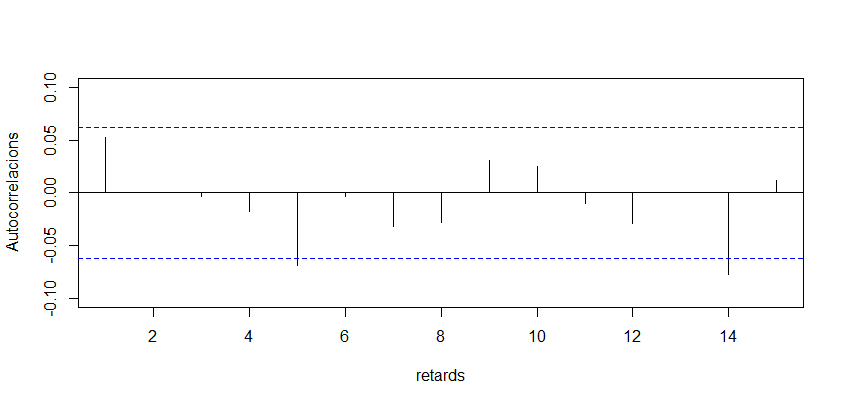
\includegraphics[width=0.48\textwidth]{figs/corrend.png}
  }
  \subfloat[Rendibilitats al quadrat\label{fig:rend2}]{
    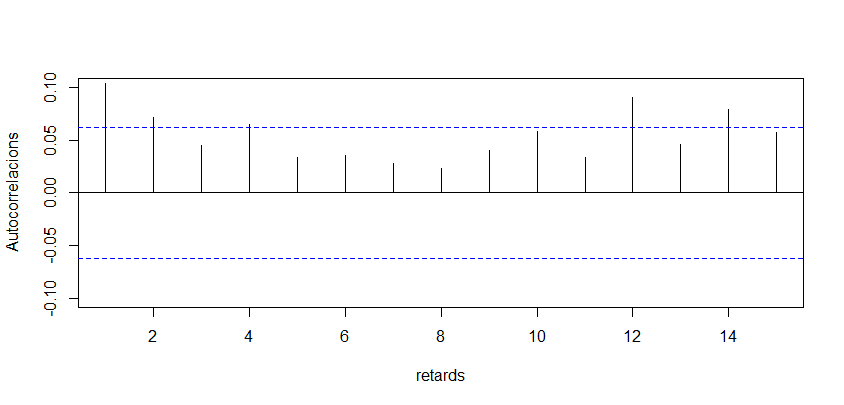
\includegraphics[width=0.48\textwidth]{figs/corrend2.png}
  }
  \caption{Autocorrelacions de les rendibilitats i rendibilitats al quadrat.}
\end{figure}
Aquests resultats eren d'esperar, ja que en general en els mercats financers les correlacions entre les rendibilitats són insignificants (excepte en escales de temps menors a 20 minuts) \cite{20}.\\
En canvi, en general, al fer una funció que anul·li el signe, com pot ser elevar al quadrat, s’observen correlacions. Això es deu en part a que esdeveniments d’alta volatilitat tendeixen a ocórrer junts, és a dir que hi ha pujades i baixades abruptes en temps curts. Aquest fet però, no el detecta la correlació directa ja que després d’una alta pujada pot haver-hi tant una altra pujada com una baixada. Ara bé, en prendre el valor absolut de les variacions, aquests dos fets no es diferencien i és aleshores quan detectem les correlacions.\\
Finalment cal remarcar que, tot i que suposar normalitat pot semblar una mica contradictori amb tenir variables aleatòries no correlacionades però dependents, veurem que això s’explica pel fet que, com veurem en la pròxima secció, les rendibilitats no són exactament normals.







\subsection{Normalitat}%Aqui fer Jarque-Bera,pearson,Kolgomorov,QQ-PPplots




\begin{figure}[H]
	\centering \sffamily \small
	% Created by tikzDevice version 0.12 on 2019-06-13 23:40:41
% !TEX encoding = UTF-8 Unicode
\begin{tikzpicture}[x=1pt,y=1pt]
\definecolor{fillColor}{RGB}{255,255,255}
\path[use as bounding box,fill=fillColor,fill opacity=0.00] (0,0) rectangle (252.94,252.94);
\begin{scope}
\path[clip] ( 48.00,  0.00) rectangle (252.94, 50.59);
\definecolor{fillColor}{RGB}{173,216,230}

\path[fill=fillColor] (142.38, 15.93) --
	(142.38, 34.66) --
	(163.94, 34.66) --
	(163.94, 15.93) --
	cycle;
\definecolor{drawColor}{RGB}{0,0,0}

\path[draw=drawColor,line width= 0.4pt,line join=round] (152.60, 15.93) -- (152.60, 34.66);

\path[draw=drawColor,line width= 0.4pt,dash pattern=on 4pt off 4pt ,line join=round,line cap=round] (110.55, 25.29) -- (142.38, 25.29);

\path[draw=drawColor,line width= 0.4pt,dash pattern=on 4pt off 4pt ,line join=round,line cap=round] (195.67, 25.29) -- (163.94, 25.29);

\path[draw=drawColor,line width= 0.4pt,line join=round,line cap=round] (110.55, 20.61) -- (110.55, 29.98);

\path[draw=drawColor,line width= 0.4pt,line join=round,line cap=round] (195.67, 20.61) -- (195.67, 29.98);
\definecolor{drawColor}{RGB}{255,255,255}

\path[draw=drawColor,line width= 0.4pt,line join=round,line cap=round] (142.38, 15.93) --
	(142.38, 34.66) --
	(163.94, 34.66) --
	(163.94, 15.93) --
	(142.38, 15.93);
\definecolor{drawColor}{gray}{0.40}

\path[draw=drawColor,line width= 0.4pt,line join=round,line cap=round] ( 83.32, 23.04) -- ( 87.82, 27.54);

\path[draw=drawColor,line width= 0.4pt,line join=round,line cap=round] ( 83.32, 27.54) -- ( 87.82, 23.04);

\path[draw=drawColor,line width= 0.4pt,line join=round,line cap=round] ( 58.33, 23.04) -- ( 62.83, 27.54);

\path[draw=drawColor,line width= 0.4pt,line join=round,line cap=round] ( 58.33, 27.54) -- ( 62.83, 23.04);

\path[draw=drawColor,line width= 0.4pt,line join=round,line cap=round] (196.02, 23.04) -- (200.52, 27.54);

\path[draw=drawColor,line width= 0.4pt,line join=round,line cap=round] (196.02, 27.54) -- (200.52, 23.04);

\path[draw=drawColor,line width= 0.4pt,line join=round,line cap=round] (194.37, 23.04) -- (198.87, 27.54);

\path[draw=drawColor,line width= 0.4pt,line join=round,line cap=round] (194.37, 27.54) -- (198.87, 23.04);

\path[draw=drawColor,line width= 0.4pt,line join=round,line cap=round] (104.79, 23.04) -- (109.29, 27.54);

\path[draw=drawColor,line width= 0.4pt,line join=round,line cap=round] (104.79, 27.54) -- (109.29, 23.04);

\path[draw=drawColor,line width= 0.4pt,line join=round,line cap=round] (194.87, 23.04) -- (199.37, 27.54);

\path[draw=drawColor,line width= 0.4pt,line join=round,line cap=round] (194.87, 27.54) -- (199.37, 23.04);

\path[draw=drawColor,line width= 0.4pt,line join=round,line cap=round] ( 70.41, 23.04) -- ( 74.91, 27.54);

\path[draw=drawColor,line width= 0.4pt,line join=round,line cap=round] ( 70.41, 27.54) -- ( 74.91, 23.04);

\path[draw=drawColor,line width= 0.4pt,line join=round,line cap=round] (213.51, 23.04) -- (218.01, 27.54);

\path[draw=drawColor,line width= 0.4pt,line join=round,line cap=round] (213.51, 27.54) -- (218.01, 23.04);

\path[draw=drawColor,line width= 0.4pt,line join=round,line cap=round] ( 93.14, 23.04) -- ( 97.64, 27.54);

\path[draw=drawColor,line width= 0.4pt,line join=round,line cap=round] ( 93.14, 27.54) -- ( 97.64, 23.04);

\path[draw=drawColor,line width= 0.4pt,line join=round,line cap=round] ( 97.71, 23.04) -- (102.21, 27.54);

\path[draw=drawColor,line width= 0.4pt,line join=round,line cap=round] ( 97.71, 27.54) -- (102.21, 23.04);

\path[draw=drawColor,line width= 0.4pt,line join=round,line cap=round] (208.39, 23.04) -- (212.89, 27.54);

\path[draw=drawColor,line width= 0.4pt,line join=round,line cap=round] (208.39, 27.54) -- (212.89, 23.04);

\path[draw=drawColor,line width= 0.4pt,line join=round,line cap=round] (106.93, 23.04) -- (111.43, 27.54);

\path[draw=drawColor,line width= 0.4pt,line join=round,line cap=round] (106.93, 27.54) -- (111.43, 23.04);

\path[draw=drawColor,line width= 0.4pt,line join=round,line cap=round] (101.68, 23.04) -- (106.18, 27.54);

\path[draw=drawColor,line width= 0.4pt,line join=round,line cap=round] (101.68, 27.54) -- (106.18, 23.04);

\path[draw=drawColor,line width= 0.4pt,line join=round,line cap=round] ( 86.49, 23.04) -- ( 90.99, 27.54);

\path[draw=drawColor,line width= 0.4pt,line join=round,line cap=round] ( 86.49, 27.54) -- ( 90.99, 23.04);

\path[draw=drawColor,line width= 0.4pt,line join=round,line cap=round] (206.90, 23.04) -- (211.40, 27.54);

\path[draw=drawColor,line width= 0.4pt,line join=round,line cap=round] (206.90, 27.54) -- (211.40, 23.04);

\path[draw=drawColor,line width= 0.4pt,line join=round,line cap=round] (201.64, 23.04) -- (206.14, 27.54);

\path[draw=drawColor,line width= 0.4pt,line join=round,line cap=round] (201.64, 27.54) -- (206.14, 23.04);

\path[draw=drawColor,line width= 0.4pt,line join=round,line cap=round] (201.24, 23.04) -- (205.74, 27.54);

\path[draw=drawColor,line width= 0.4pt,line join=round,line cap=round] (201.24, 27.54) -- (205.74, 23.04);

\path[draw=drawColor,line width= 0.4pt,line join=round,line cap=round] ( 98.97, 23.04) -- (103.47, 27.54);

\path[draw=drawColor,line width= 0.4pt,line join=round,line cap=round] ( 98.97, 27.54) -- (103.47, 23.04);

\path[draw=drawColor,line width= 0.4pt,line join=round,line cap=round] (198.05, 23.04) -- (202.55, 27.54);

\path[draw=drawColor,line width= 0.4pt,line join=round,line cap=round] (198.05, 27.54) -- (202.55, 23.04);

\path[draw=drawColor,line width= 0.4pt,line join=round,line cap=round] (105.99, 23.04) -- (110.49, 27.54);

\path[draw=drawColor,line width= 0.4pt,line join=round,line cap=round] (105.99, 27.54) -- (110.49, 23.04);

\path[draw=drawColor,line width= 0.4pt,line join=round,line cap=round] ( 65.58, 23.04) -- ( 70.08, 27.54);

\path[draw=drawColor,line width= 0.4pt,line join=round,line cap=round] ( 65.58, 27.54) -- ( 70.08, 23.04);

\path[draw=drawColor,line width= 0.4pt,line join=round,line cap=round] (211.91, 23.04) -- (216.41, 27.54);

\path[draw=drawColor,line width= 0.4pt,line join=round,line cap=round] (211.91, 27.54) -- (216.41, 23.04);

\path[draw=drawColor,line width= 0.4pt,line join=round,line cap=round] (203.89, 23.04) -- (208.39, 27.54);

\path[draw=drawColor,line width= 0.4pt,line join=round,line cap=round] (203.89, 27.54) -- (208.39, 23.04);

\path[draw=drawColor,line width= 0.4pt,line join=round,line cap=round] (241.26, 23.04) -- (245.76, 27.54);

\path[draw=drawColor,line width= 0.4pt,line join=round,line cap=round] (241.26, 27.54) -- (245.76, 23.04);

\path[draw=drawColor,line width= 0.4pt,line join=round,line cap=round] ( 96.21, 23.04) -- (100.71, 27.54);

\path[draw=drawColor,line width= 0.4pt,line join=round,line cap=round] ( 96.21, 27.54) -- (100.71, 23.04);

\path[draw=drawColor,line width= 0.4pt,line join=round,line cap=round] (243.10, 23.04) -- (247.60, 27.54);

\path[draw=drawColor,line width= 0.4pt,line join=round,line cap=round] (243.10, 27.54) -- (247.60, 23.04);

\path[draw=drawColor,line width= 0.4pt,line join=round,line cap=round] (220.30, 23.04) -- (224.80, 27.54);

\path[draw=drawColor,line width= 0.4pt,line join=round,line cap=round] (220.30, 27.54) -- (224.80, 23.04);

\path[draw=drawColor,line width= 0.4pt,line join=round,line cap=round] (209.83, 23.04) -- (214.33, 27.54);

\path[draw=drawColor,line width= 0.4pt,line join=round,line cap=round] (209.83, 27.54) -- (214.33, 23.04);

\path[draw=drawColor,line width= 0.4pt,line join=round,line cap=round] ( 98.92, 23.04) -- (103.42, 27.54);

\path[draw=drawColor,line width= 0.4pt,line join=round,line cap=round] ( 98.92, 27.54) -- (103.42, 23.04);

\path[draw=drawColor,line width= 0.4pt,line join=round,line cap=round] ( 81.61, 23.04) -- ( 86.11, 27.54);

\path[draw=drawColor,line width= 0.4pt,line join=round,line cap=round] ( 81.61, 27.54) -- ( 86.11, 23.04);

\path[draw=drawColor,line width= 0.4pt,line join=round,line cap=round] ( 98.39, 23.04) -- (102.89, 27.54);

\path[draw=drawColor,line width= 0.4pt,line join=round,line cap=round] ( 98.39, 27.54) -- (102.89, 23.04);

\path[draw=drawColor,line width= 0.4pt,line join=round,line cap=round] ( 77.68, 23.04) -- ( 82.18, 27.54);

\path[draw=drawColor,line width= 0.4pt,line join=round,line cap=round] ( 77.68, 27.54) -- ( 82.18, 23.04);

\path[draw=drawColor,line width= 0.4pt,line join=round,line cap=round] (106.59, 23.04) -- (111.09, 27.54);

\path[draw=drawColor,line width= 0.4pt,line join=round,line cap=round] (106.59, 27.54) -- (111.09, 23.04);

\path[draw=drawColor,line width= 0.4pt,line join=round,line cap=round] ( 71.28, 23.04) -- ( 75.78, 27.54);

\path[draw=drawColor,line width= 0.4pt,line join=round,line cap=round] ( 71.28, 27.54) -- ( 75.78, 23.04);

\path[draw=drawColor,line width= 0.4pt,line join=round,line cap=round] (104.69, 23.04) -- (109.19, 27.54);

\path[draw=drawColor,line width= 0.4pt,line join=round,line cap=round] (104.69, 27.54) -- (109.19, 23.04);

\path[draw=drawColor,line width= 0.4pt,line join=round,line cap=round] (199.52, 23.04) -- (204.02, 27.54);

\path[draw=drawColor,line width= 0.4pt,line join=round,line cap=round] (199.52, 27.54) -- (204.02, 23.04);

\path[draw=drawColor,line width= 0.4pt,line join=round,line cap=round] (104.19, 23.04) -- (108.69, 27.54);

\path[draw=drawColor,line width= 0.4pt,line join=round,line cap=round] (104.19, 27.54) -- (108.69, 23.04);

\path[draw=drawColor,line width= 0.4pt,line join=round,line cap=round] (101.86, 23.04) -- (106.36, 27.54);

\path[draw=drawColor,line width= 0.4pt,line join=round,line cap=round] (101.86, 27.54) -- (106.36, 23.04);

\path[draw=drawColor,line width= 0.4pt,line join=round,line cap=round] (100.85, 23.04) -- (105.35, 27.54);

\path[draw=drawColor,line width= 0.4pt,line join=round,line cap=round] (100.85, 27.54) -- (105.35, 23.04);

\path[draw=drawColor,line width= 0.4pt,line join=round,line cap=round] ( 53.34, 23.04) -- ( 57.84, 27.54);

\path[draw=drawColor,line width= 0.4pt,line join=round,line cap=round] ( 53.34, 27.54) -- ( 57.84, 23.04);

\path[draw=drawColor,line width= 0.4pt,line join=round,line cap=round] ( 79.39, 23.04) -- ( 83.89, 27.54);

\path[draw=drawColor,line width= 0.4pt,line join=round,line cap=round] ( 79.39, 27.54) -- ( 83.89, 23.04);

\path[draw=drawColor,line width= 0.4pt,line join=round,line cap=round] (203.72, 23.04) -- (208.22, 27.54);

\path[draw=drawColor,line width= 0.4pt,line join=round,line cap=round] (203.72, 27.54) -- (208.22, 23.04);

\path[draw=drawColor,line width= 0.4pt,line join=round,line cap=round] (107.36, 23.04) -- (111.86, 27.54);

\path[draw=drawColor,line width= 0.4pt,line join=round,line cap=round] (107.36, 27.54) -- (111.86, 23.04);

\path[draw=drawColor,line width= 0.4pt,line join=round,line cap=round] (209.48, 23.04) -- (213.98, 27.54);

\path[draw=drawColor,line width= 0.4pt,line join=round,line cap=round] (209.48, 27.54) -- (213.98, 23.04);

\path[draw=drawColor,line width= 0.4pt,line join=round,line cap=round] (200.36, 23.04) -- (204.86, 27.54);

\path[draw=drawColor,line width= 0.4pt,line join=round,line cap=round] (200.36, 27.54) -- (204.86, 23.04);

\path[draw=drawColor,line width= 0.4pt,line join=round,line cap=round] ( 61.68, 23.04) -- ( 66.18, 27.54);

\path[draw=drawColor,line width= 0.4pt,line join=round,line cap=round] ( 61.68, 27.54) -- ( 66.18, 23.04);

\path[draw=drawColor,line width= 0.4pt,line join=round,line cap=round] (102.95, 23.04) -- (107.45, 27.54);

\path[draw=drawColor,line width= 0.4pt,line join=round,line cap=round] (102.95, 27.54) -- (107.45, 23.04);

\path[draw=drawColor,line width= 0.4pt,line join=round,line cap=round] (229.54, 23.04) -- (234.04, 27.54);

\path[draw=drawColor,line width= 0.4pt,line join=round,line cap=round] (229.54, 27.54) -- (234.04, 23.04);
\end{scope}
\begin{scope}
\path[clip] (  0.00, 50.59) rectangle (252.94,252.94);
\definecolor{drawColor}{RGB}{0,0,0}

\node[text=drawColor,anchor=base,inner sep=0pt, outer sep=0pt, scale=  1.20] at (150.47,230.80) {\bfseries Distribució de les rendibilitats diàries};

\node[text=drawColor,rotate= 90.00,anchor=base,inner sep=0pt, outer sep=0pt, scale=  1.00] at (  9.60,139.77) {Densitat};
\end{scope}
\begin{scope}
\path[clip] (  0.00,  0.00) rectangle (252.94,252.94);
\definecolor{drawColor}{RGB}{0,0,0}

\path[draw=drawColor,line width= 0.4pt,line join=round,line cap=round] ( 55.59, 62.59) -- (245.35, 62.59);

\path[draw=drawColor,line width= 0.4pt,line join=round,line cap=round] ( 55.59, 62.59) -- ( 55.59, 56.59);

\path[draw=drawColor,line width= 0.4pt,line join=round,line cap=round] (103.03, 62.59) -- (103.03, 56.59);

\path[draw=drawColor,line width= 0.4pt,line join=round,line cap=round] (150.47, 62.59) -- (150.47, 56.59);

\path[draw=drawColor,line width= 0.4pt,line join=round,line cap=round] (197.91, 62.59) -- (197.91, 56.59);

\path[draw=drawColor,line width= 0.4pt,line join=round,line cap=round] (245.35, 62.59) -- (245.35, 56.59);

\node[text=drawColor,anchor=base,inner sep=0pt, outer sep=0pt, scale=  1.00] at ( 55.59, 40.99) {-0.10};

\node[text=drawColor,anchor=base,inner sep=0pt, outer sep=0pt, scale=  1.00] at (103.03, 40.99) {-0.05};

\node[text=drawColor,anchor=base,inner sep=0pt, outer sep=0pt, scale=  1.00] at (150.47, 40.99) {0.00};

\node[text=drawColor,anchor=base,inner sep=0pt, outer sep=0pt, scale=  1.00] at (197.91, 40.99) {0.05};

\node[text=drawColor,anchor=base,inner sep=0pt, outer sep=0pt, scale=  1.00] at (245.35, 40.99) {0.10};

\path[draw=drawColor,line width= 0.4pt,line join=round,line cap=round] ( 48.00, 68.31) -- ( 48.00,211.23);

\path[draw=drawColor,line width= 0.4pt,line join=round,line cap=round] ( 48.00, 68.31) -- ( 42.00, 68.31);

\path[draw=drawColor,line width= 0.4pt,line join=round,line cap=round] ( 48.00, 92.13) -- ( 42.00, 92.13);

\path[draw=drawColor,line width= 0.4pt,line join=round,line cap=round] ( 48.00,115.95) -- ( 42.00,115.95);

\path[draw=drawColor,line width= 0.4pt,line join=round,line cap=round] ( 48.00,139.77) -- ( 42.00,139.77);

\path[draw=drawColor,line width= 0.4pt,line join=round,line cap=round] ( 48.00,163.59) -- ( 42.00,163.59);

\path[draw=drawColor,line width= 0.4pt,line join=round,line cap=round] ( 48.00,187.41) -- ( 42.00,187.41);

\path[draw=drawColor,line width= 0.4pt,line join=round,line cap=round] ( 48.00,211.23) -- ( 42.00,211.23);

\node[text=drawColor,rotate= 90.00,anchor=base,inner sep=0pt, outer sep=0pt, scale=  1.00] at ( 33.60, 68.31) {0};

\node[text=drawColor,rotate= 90.00,anchor=base,inner sep=0pt, outer sep=0pt, scale=  1.00] at ( 33.60, 92.13) {5};

\node[text=drawColor,rotate= 90.00,anchor=base,inner sep=0pt, outer sep=0pt, scale=  1.00] at ( 33.60,115.95) {10};

\node[text=drawColor,rotate= 90.00,anchor=base,inner sep=0pt, outer sep=0pt, scale=  1.00] at ( 33.60,139.77) {15};

\node[text=drawColor,rotate= 90.00,anchor=base,inner sep=0pt, outer sep=0pt, scale=  1.00] at ( 33.60,163.59) {20};

\node[text=drawColor,rotate= 90.00,anchor=base,inner sep=0pt, outer sep=0pt, scale=  1.00] at ( 33.60,187.41) {25};

\node[text=drawColor,rotate= 90.00,anchor=base,inner sep=0pt, outer sep=0pt, scale=  1.00] at ( 33.60,211.23) {30};
\end{scope}
\begin{scope}
\path[clip] ( 48.00, 62.59) rectangle (252.94,216.94);
\definecolor{fillColor}{RGB}{173,216,230}

\path[fill=fillColor] ( 74.57, 68.31) rectangle ( 84.06, 69.73);

\path[fill=fillColor] ( 84.06, 68.31) rectangle ( 93.54, 69.73);

\path[fill=fillColor] ( 93.54, 68.31) rectangle (103.03, 70.68);

\path[fill=fillColor] (103.03, 68.31) rectangle (112.52, 71.15);

\path[fill=fillColor] (112.52, 68.31) rectangle (122.01, 77.80);

\path[fill=fillColor] (122.01, 68.31) rectangle (131.50, 92.98);

\path[fill=fillColor] (131.50, 68.31) rectangle (140.98,126.67);

\path[fill=fillColor] (140.98, 68.31) rectangle (150.47,202.59);

\path[fill=fillColor] (150.47, 68.31) rectangle (159.96,195.47);

\path[fill=fillColor] (159.96, 68.31) rectangle (169.45,135.21);

\path[fill=fillColor] (169.45, 68.31) rectangle (178.94, 99.62);

\path[fill=fillColor] (178.94, 68.31) rectangle (188.43, 76.85);

\path[fill=fillColor] (188.43, 68.31) rectangle (197.91, 73.05);

\path[fill=fillColor] (197.91, 68.31) rectangle (207.40, 69.73);

\path[fill=fillColor] (207.40, 68.31) rectangle (216.89, 68.78);

\path[fill=fillColor] (216.89, 68.31) rectangle (226.38, 69.25);
\definecolor{drawColor}{RGB}{218,112,214}

\path[draw=drawColor,line width= 1.2pt,dash pattern=on 1pt off 3pt ,line join=round,line cap=round] ( 55.59, 68.31) --
	( 57.49, 68.31) --
	( 59.39, 68.31) --
	( 61.28, 68.31) --
	( 63.18, 68.31) --
	( 65.08, 68.31) --
	( 66.98, 68.31) --
	( 68.87, 68.31) --
	( 70.77, 68.31) --
	( 72.67, 68.31) --
	( 74.57, 68.31) --
	( 76.46, 68.31) --
	( 78.36, 68.31) --
	( 80.26, 68.31) --
	( 82.16, 68.32) --
	( 84.06, 68.33) --
	( 85.95, 68.34) --
	( 87.85, 68.36) --
	( 89.75, 68.39) --
	( 91.65, 68.43) --
	( 93.54, 68.50) --
	( 95.44, 68.60) --
	( 97.34, 68.75) --
	( 99.24, 68.96) --
	(101.13, 69.25) --
	(103.03, 69.66) --
	(104.93, 70.22) --
	(106.83, 70.96) --
	(108.72, 71.95) --
	(110.62, 73.24) --
	(112.52, 74.89) --
	(114.42, 76.97) --
	(116.31, 79.55) --
	(118.21, 82.69) --
	(120.11, 86.46) --
	(122.01, 90.89) --
	(123.91, 96.02) --
	(125.80,101.85) --
	(127.70,108.33) --
	(129.60,115.40) --
	(131.50,122.96) --
	(133.39,130.85) --
	(135.29,138.88) --
	(137.19,146.85) --
	(139.09,154.50) --
	(140.98,161.58) --
	(142.88,167.85) --
	(144.78,173.06) --
	(146.68,177.02) --
	(148.57,179.56) --
	(150.47,180.58) --
	(152.37,180.04) --
	(154.27,177.97) --
	(156.17,174.43) --
	(158.06,169.59) --
	(159.96,163.63) --
	(161.86,156.78) --
	(163.76,149.28) --
	(165.65,141.38) --
	(167.55,133.35) --
	(169.45,125.39) --
	(171.35,117.71) --
	(173.24,110.47) --
	(175.14,103.80) --
	(177.04, 97.76) --
	(178.94, 92.42) --
	(180.83, 87.77) --
	(182.73, 83.80) --
	(184.63, 80.46) --
	(186.53, 77.72) --
	(188.43, 75.49) --
	(190.32, 73.71) --
	(192.22, 72.32) --
	(194.12, 71.24) --
	(196.02, 70.43) --
	(197.91, 69.82) --
	(199.81, 69.37) --
	(201.71, 69.04) --
	(203.61, 68.81) --
	(205.50, 68.64) --
	(207.40, 68.53) --
	(209.30, 68.45) --
	(211.20, 68.40) --
	(213.09, 68.37) --
	(214.99, 68.34) --
	(216.89, 68.33) --
	(218.79, 68.32) --
	(220.69, 68.31) --
	(222.58, 68.31) --
	(224.48, 68.31) --
	(226.38, 68.31) --
	(228.28, 68.31) --
	(230.17, 68.31) --
	(232.07, 68.31) --
	(233.97, 68.31) --
	(235.87, 68.31) --
	(237.76, 68.31) --
	(239.66, 68.31) --
	(241.56, 68.31) --
	(243.46, 68.31) --
	(245.35, 68.31);
\definecolor{drawColor}{RGB}{50,205,50}

\path[draw=drawColor,line width= 1.2pt,dash pattern=on 1pt off 3pt ,line join=round,line cap=round] ( 55.59, 68.35) --
	( 57.49, 68.36) --
	( 59.39, 68.37) --
	( 61.28, 68.38) --
	( 63.18, 68.40) --
	( 65.08, 68.41) --
	( 66.98, 68.43) --
	( 68.87, 68.45) --
	( 70.77, 68.47) --
	( 72.67, 68.50) --
	( 74.57, 68.53) --
	( 76.46, 68.57) --
	( 78.36, 68.62) --
	( 80.26, 68.67) --
	( 82.16, 68.73) --
	( 84.06, 68.81) --
	( 85.95, 68.89) --
	( 87.85, 69.00) --
	( 89.75, 69.12) --
	( 91.65, 69.27) --
	( 93.54, 69.44) --
	( 95.44, 69.64) --
	( 97.34, 69.89) --
	( 99.24, 70.18) --
	(101.13, 70.52) --
	(103.03, 70.94) --
	(104.93, 71.43) --
	(106.83, 72.03) --
	(108.72, 72.74) --
	(110.62, 73.60) --
	(112.52, 74.63) --
	(114.42, 75.87) --
	(116.31, 77.38) --
	(118.21, 79.20) --
	(120.11, 81.40) --
	(122.01, 84.07) --
	(123.91, 87.30) --
	(125.80, 91.22) --
	(127.70, 95.95) --
	(129.60,101.66) --
	(131.50,108.50) --
	(133.39,116.63) --
	(135.29,126.19) --
	(137.19,137.22) --
	(139.09,149.64) --
	(140.98,163.12) --
	(142.88,177.01) --
	(144.78,190.30) --
	(146.68,201.64) --
	(148.57,209.58) --
	(150.47,212.94) --
	(152.37,211.16) --
	(154.27,204.54) --
	(156.17,194.11) --
	(158.06,181.27) --
	(159.96,167.44) --
	(161.86,153.75) --
	(163.76,140.95) --
	(165.65,129.47) --
	(167.55,119.45) --
	(169.45,110.88) --
	(171.35,103.66) --
	(173.24, 97.62) --
	(175.14, 92.60) --
	(177.04, 88.44) --
	(178.94, 85.01) --
	(180.83, 82.17) --
	(182.73, 79.84) --
	(184.63, 77.91) --
	(186.53, 76.31) --
	(188.43, 74.99) --
	(190.32, 73.90) --
	(192.22, 72.99) --
	(194.12, 72.23) --
	(196.02, 71.61) --
	(197.91, 71.08) --
	(199.81, 70.64) --
	(201.71, 70.28) --
	(203.61, 69.97) --
	(205.50, 69.71) --
	(207.40, 69.50) --
	(209.30, 69.32) --
	(211.20, 69.16) --
	(213.09, 69.03) --
	(214.99, 68.93) --
	(216.89, 68.83) --
	(218.79, 68.75) --
	(220.69, 68.69) --
	(222.58, 68.63) --
	(224.48, 68.58) --
	(226.38, 68.54) --
	(228.28, 68.51) --
	(230.17, 68.48) --
	(232.07, 68.46) --
	(233.97, 68.43) --
	(235.87, 68.42) --
	(237.76, 68.40) --
	(239.66, 68.39) --
	(241.56, 68.38) --
	(243.46, 68.37) --
	(245.35, 68.36);

\path[] ( 54.15,212.31) rectangle (127.17,176.31);
\definecolor{drawColor}{RGB}{218,112,214}

\path[draw=drawColor,line width= 1.6pt,dash pattern=on 1pt off 3pt ,line join=round,line cap=round] ( 63.15,200.31) -- ( 81.15,200.31);
\definecolor{drawColor}{RGB}{50,205,50}

\path[draw=drawColor,line width= 1.6pt,dash pattern=on 1pt off 3pt ,line join=round,line cap=round] ( 63.15,188.31) -- ( 81.15,188.31);
\definecolor{drawColor}{RGB}{0,0,0}

\node[text=drawColor,anchor=base west,inner sep=0pt, outer sep=0pt, scale=  1.00] at ( 90.15,196.87) {Normal};

\node[text=drawColor,anchor=base west,inner sep=0pt, outer sep=0pt, scale=  1.00] at ( 90.15,184.87) {NIG};
\end{scope}
\end{tikzpicture}

	\caption{Evolució del preu de tancament de Caterpillar entre 2015 i 2018}
	\label{fig:distribucio rendibilitats}
\end{figure}
\begin{figure}[H]
	\centering \sffamily \small
	% Created by tikzDevice version 0.12 on 2019-06-13 19:48:56
% !TEX encoding = UTF-8 Unicode
\begin{tikzpicture}[x=1pt,y=1pt]
\definecolor{fillColor}{RGB}{255,255,255}
\path[use as bounding box,fill=fillColor,fill opacity=0.00] (0,0) rectangle (361.35,180.67);
\begin{scope}
\path[clip] ( 48.00, 48.00) rectangle (174.67,156.67);
\definecolor{drawColor}{gray}{0.40}

\path[draw=drawColor,line width= 0.4pt,line join=round,line cap=round] ( 50.44, 49.77) -- ( 54.94, 54.27);

\path[draw=drawColor,line width= 0.4pt,line join=round,line cap=round] ( 50.44, 54.27) -- ( 54.94, 49.77);

\path[draw=drawColor,line width= 0.4pt,line join=round,line cap=round] ( 50.56, 49.80) -- ( 55.06, 54.30);

\path[draw=drawColor,line width= 0.4pt,line join=round,line cap=round] ( 50.56, 54.30) -- ( 55.06, 49.80);

\path[draw=drawColor,line width= 0.4pt,line join=round,line cap=round] ( 50.68, 49.82) -- ( 55.18, 54.32);

\path[draw=drawColor,line width= 0.4pt,line join=round,line cap=round] ( 50.68, 54.32) -- ( 55.18, 49.82);

\path[draw=drawColor,line width= 0.4pt,line join=round,line cap=round] ( 50.79, 49.86) -- ( 55.29, 54.36);

\path[draw=drawColor,line width= 0.4pt,line join=round,line cap=round] ( 50.79, 54.36) -- ( 55.29, 49.86);

\path[draw=drawColor,line width= 0.4pt,line join=round,line cap=round] ( 50.91, 49.91) -- ( 55.41, 54.41);

\path[draw=drawColor,line width= 0.4pt,line join=round,line cap=round] ( 50.91, 54.41) -- ( 55.41, 49.91);

\path[draw=drawColor,line width= 0.4pt,line join=round,line cap=round] ( 51.03, 49.92) -- ( 55.53, 54.42);

\path[draw=drawColor,line width= 0.4pt,line join=round,line cap=round] ( 51.03, 54.42) -- ( 55.53, 49.92);

\path[draw=drawColor,line width= 0.4pt,line join=round,line cap=round] ( 51.14, 50.03) -- ( 55.64, 54.53);

\path[draw=drawColor,line width= 0.4pt,line join=round,line cap=round] ( 51.14, 54.53) -- ( 55.64, 50.03);

\path[draw=drawColor,line width= 0.4pt,line join=round,line cap=round] ( 51.26, 50.07) -- ( 55.76, 54.57);

\path[draw=drawColor,line width= 0.4pt,line join=round,line cap=round] ( 51.26, 54.57) -- ( 55.76, 50.07);

\path[draw=drawColor,line width= 0.4pt,line join=round,line cap=round] ( 51.38, 50.13) -- ( 55.88, 54.63);

\path[draw=drawColor,line width= 0.4pt,line join=round,line cap=round] ( 51.38, 54.63) -- ( 55.88, 50.13);

\path[draw=drawColor,line width= 0.4pt,line join=round,line cap=round] ( 51.49, 50.18) -- ( 55.99, 54.68);

\path[draw=drawColor,line width= 0.4pt,line join=round,line cap=round] ( 51.49, 54.68) -- ( 55.99, 50.18);

\path[draw=drawColor,line width= 0.4pt,line join=round,line cap=round] ( 51.61, 50.29) -- ( 56.11, 54.79);

\path[draw=drawColor,line width= 0.4pt,line join=round,line cap=round] ( 51.61, 54.79) -- ( 56.11, 50.29);

\path[draw=drawColor,line width= 0.4pt,line join=round,line cap=round] ( 51.73, 50.63) -- ( 56.23, 55.13);

\path[draw=drawColor,line width= 0.4pt,line join=round,line cap=round] ( 51.73, 55.13) -- ( 56.23, 50.63);

\path[draw=drawColor,line width= 0.4pt,line join=round,line cap=round] ( 51.84, 50.84) -- ( 56.34, 55.34);

\path[draw=drawColor,line width= 0.4pt,line join=round,line cap=round] ( 51.84, 55.34) -- ( 56.34, 50.84);

\path[draw=drawColor,line width= 0.4pt,line join=round,line cap=round] ( 51.96, 50.96) -- ( 56.46, 55.46);

\path[draw=drawColor,line width= 0.4pt,line join=round,line cap=round] ( 51.96, 55.46) -- ( 56.46, 50.96);

\path[draw=drawColor,line width= 0.4pt,line join=round,line cap=round] ( 52.08, 51.02) -- ( 56.58, 55.52);

\path[draw=drawColor,line width= 0.4pt,line join=round,line cap=round] ( 52.08, 55.52) -- ( 56.58, 51.02);

\path[draw=drawColor,line width= 0.4pt,line join=round,line cap=round] ( 52.20, 51.07) -- ( 56.70, 55.57);

\path[draw=drawColor,line width= 0.4pt,line join=round,line cap=round] ( 52.20, 55.57) -- ( 56.70, 51.07);

\path[draw=drawColor,line width= 0.4pt,line join=round,line cap=round] ( 52.31, 51.08) -- ( 56.81, 55.58);

\path[draw=drawColor,line width= 0.4pt,line join=round,line cap=round] ( 52.31, 55.58) -- ( 56.81, 51.08);

\path[draw=drawColor,line width= 0.4pt,line join=round,line cap=round] ( 52.43, 51.27) -- ( 56.93, 55.77);

\path[draw=drawColor,line width= 0.4pt,line join=round,line cap=round] ( 52.43, 55.77) -- ( 56.93, 51.27);

\path[draw=drawColor,line width= 0.4pt,line join=round,line cap=round] ( 52.55, 51.36) -- ( 57.05, 55.86);

\path[draw=drawColor,line width= 0.4pt,line join=round,line cap=round] ( 52.55, 55.86) -- ( 57.05, 51.36);

\path[draw=drawColor,line width= 0.4pt,line join=round,line cap=round] ( 52.66, 51.38) -- ( 57.16, 55.88);

\path[draw=drawColor,line width= 0.4pt,line join=round,line cap=round] ( 52.66, 55.88) -- ( 57.16, 51.38);

\path[draw=drawColor,line width= 0.4pt,line join=round,line cap=round] ( 52.78, 51.52) -- ( 57.28, 56.02);

\path[draw=drawColor,line width= 0.4pt,line join=round,line cap=round] ( 52.78, 56.02) -- ( 57.28, 51.52);

\path[draw=drawColor,line width= 0.4pt,line join=round,line cap=round] ( 52.90, 51.68) -- ( 57.40, 56.18);

\path[draw=drawColor,line width= 0.4pt,line join=round,line cap=round] ( 52.90, 56.18) -- ( 57.40, 51.68);

\path[draw=drawColor,line width= 0.4pt,line join=round,line cap=round] ( 53.01, 51.75) -- ( 57.51, 56.25);

\path[draw=drawColor,line width= 0.4pt,line join=round,line cap=round] ( 53.01, 56.25) -- ( 57.51, 51.75);

\path[draw=drawColor,line width= 0.4pt,line join=round,line cap=round] ( 53.13, 51.77) -- ( 57.63, 56.27);

\path[draw=drawColor,line width= 0.4pt,line join=round,line cap=round] ( 53.13, 56.27) -- ( 57.63, 51.77);

\path[draw=drawColor,line width= 0.4pt,line join=round,line cap=round] ( 53.25, 51.95) -- ( 57.75, 56.45);

\path[draw=drawColor,line width= 0.4pt,line join=round,line cap=round] ( 53.25, 56.45) -- ( 57.75, 51.95);

\path[draw=drawColor,line width= 0.4pt,line join=round,line cap=round] ( 53.37, 52.05) -- ( 57.87, 56.55);

\path[draw=drawColor,line width= 0.4pt,line join=round,line cap=round] ( 53.37, 56.55) -- ( 57.87, 52.05);

\path[draw=drawColor,line width= 0.4pt,line join=round,line cap=round] ( 53.48, 52.10) -- ( 57.98, 56.60);

\path[draw=drawColor,line width= 0.4pt,line join=round,line cap=round] ( 53.48, 56.60) -- ( 57.98, 52.10);

\path[draw=drawColor,line width= 0.4pt,line join=round,line cap=round] ( 53.60, 52.18) -- ( 58.10, 56.68);

\path[draw=drawColor,line width= 0.4pt,line join=round,line cap=round] ( 53.60, 56.68) -- ( 58.10, 52.18);

\path[draw=drawColor,line width= 0.4pt,line join=round,line cap=round] ( 53.72, 52.35) -- ( 58.22, 56.85);

\path[draw=drawColor,line width= 0.4pt,line join=round,line cap=round] ( 53.72, 56.85) -- ( 58.22, 52.35);

\path[draw=drawColor,line width= 0.4pt,line join=round,line cap=round] ( 53.83, 52.44) -- ( 58.33, 56.94);

\path[draw=drawColor,line width= 0.4pt,line join=round,line cap=round] ( 53.83, 56.94) -- ( 58.33, 52.44);

\path[draw=drawColor,line width= 0.4pt,line join=round,line cap=round] ( 53.95, 52.46) -- ( 58.45, 56.96);

\path[draw=drawColor,line width= 0.4pt,line join=round,line cap=round] ( 53.95, 56.96) -- ( 58.45, 52.46);

\path[draw=drawColor,line width= 0.4pt,line join=round,line cap=round] ( 54.07, 52.60) -- ( 58.57, 57.10);

\path[draw=drawColor,line width= 0.4pt,line join=round,line cap=round] ( 54.07, 57.10) -- ( 58.57, 52.60);

\path[draw=drawColor,line width= 0.4pt,line join=round,line cap=round] ( 54.18, 52.76) -- ( 58.68, 57.26);

\path[draw=drawColor,line width= 0.4pt,line join=round,line cap=round] ( 54.18, 57.26) -- ( 58.68, 52.76);

\path[draw=drawColor,line width= 0.4pt,line join=round,line cap=round] ( 54.30, 52.94) -- ( 58.80, 57.44);

\path[draw=drawColor,line width= 0.4pt,line join=round,line cap=round] ( 54.30, 57.44) -- ( 58.80, 52.94);

\path[draw=drawColor,line width= 0.4pt,line join=round,line cap=round] ( 54.42, 53.10) -- ( 58.92, 57.60);

\path[draw=drawColor,line width= 0.4pt,line join=round,line cap=round] ( 54.42, 57.60) -- ( 58.92, 53.10);

\path[draw=drawColor,line width= 0.4pt,line join=round,line cap=round] ( 54.53, 53.32) -- ( 59.03, 57.82);

\path[draw=drawColor,line width= 0.4pt,line join=round,line cap=round] ( 54.53, 57.82) -- ( 59.03, 53.32);

\path[draw=drawColor,line width= 0.4pt,line join=round,line cap=round] ( 54.65, 53.40) -- ( 59.15, 57.90);

\path[draw=drawColor,line width= 0.4pt,line join=round,line cap=round] ( 54.65, 57.90) -- ( 59.15, 53.40);

\path[draw=drawColor,line width= 0.4pt,line join=round,line cap=round] ( 54.77, 53.48) -- ( 59.27, 57.98);

\path[draw=drawColor,line width= 0.4pt,line join=round,line cap=round] ( 54.77, 57.98) -- ( 59.27, 53.48);

\path[draw=drawColor,line width= 0.4pt,line join=round,line cap=round] ( 54.89, 53.54) -- ( 59.39, 58.04);

\path[draw=drawColor,line width= 0.4pt,line join=round,line cap=round] ( 54.89, 58.04) -- ( 59.39, 53.54);

\path[draw=drawColor,line width= 0.4pt,line join=round,line cap=round] ( 55.00, 53.62) -- ( 59.50, 58.12);

\path[draw=drawColor,line width= 0.4pt,line join=round,line cap=round] ( 55.00, 58.12) -- ( 59.50, 53.62);

\path[draw=drawColor,line width= 0.4pt,line join=round,line cap=round] ( 55.12, 53.73) -- ( 59.62, 58.23);

\path[draw=drawColor,line width= 0.4pt,line join=round,line cap=round] ( 55.12, 58.23) -- ( 59.62, 53.73);

\path[draw=drawColor,line width= 0.4pt,line join=round,line cap=round] ( 55.24, 53.85) -- ( 59.74, 58.35);

\path[draw=drawColor,line width= 0.4pt,line join=round,line cap=round] ( 55.24, 58.35) -- ( 59.74, 53.85);

\path[draw=drawColor,line width= 0.4pt,line join=round,line cap=round] ( 55.35, 53.97) -- ( 59.85, 58.47);

\path[draw=drawColor,line width= 0.4pt,line join=round,line cap=round] ( 55.35, 58.47) -- ( 59.85, 53.97);

\path[draw=drawColor,line width= 0.4pt,line join=round,line cap=round] ( 55.47, 54.02) -- ( 59.97, 58.52);

\path[draw=drawColor,line width= 0.4pt,line join=round,line cap=round] ( 55.47, 58.52) -- ( 59.97, 54.02);

\path[draw=drawColor,line width= 0.4pt,line join=round,line cap=round] ( 55.59, 54.12) -- ( 60.09, 58.62);

\path[draw=drawColor,line width= 0.4pt,line join=round,line cap=round] ( 55.59, 58.62) -- ( 60.09, 54.12);

\path[draw=drawColor,line width= 0.4pt,line join=round,line cap=round] ( 55.70, 54.21) -- ( 60.20, 58.71);

\path[draw=drawColor,line width= 0.4pt,line join=round,line cap=round] ( 55.70, 58.71) -- ( 60.20, 54.21);

\path[draw=drawColor,line width= 0.4pt,line join=round,line cap=round] ( 55.82, 54.24) -- ( 60.32, 58.74);

\path[draw=drawColor,line width= 0.4pt,line join=round,line cap=round] ( 55.82, 58.74) -- ( 60.32, 54.24);

\path[draw=drawColor,line width= 0.4pt,line join=round,line cap=round] ( 55.94, 54.41) -- ( 60.44, 58.91);

\path[draw=drawColor,line width= 0.4pt,line join=round,line cap=round] ( 55.94, 58.91) -- ( 60.44, 54.41);

\path[draw=drawColor,line width= 0.4pt,line join=round,line cap=round] ( 56.05, 54.45) -- ( 60.55, 58.95);

\path[draw=drawColor,line width= 0.4pt,line join=round,line cap=round] ( 56.05, 58.95) -- ( 60.55, 54.45);

\path[draw=drawColor,line width= 0.4pt,line join=round,line cap=round] ( 56.17, 54.52) -- ( 60.67, 59.02);

\path[draw=drawColor,line width= 0.4pt,line join=round,line cap=round] ( 56.17, 59.02) -- ( 60.67, 54.52);

\path[draw=drawColor,line width= 0.4pt,line join=round,line cap=round] ( 56.29, 54.61) -- ( 60.79, 59.11);

\path[draw=drawColor,line width= 0.4pt,line join=round,line cap=round] ( 56.29, 59.11) -- ( 60.79, 54.61);

\path[draw=drawColor,line width= 0.4pt,line join=round,line cap=round] ( 56.41, 54.69) -- ( 60.91, 59.19);

\path[draw=drawColor,line width= 0.4pt,line join=round,line cap=round] ( 56.41, 59.19) -- ( 60.91, 54.69);

\path[draw=drawColor,line width= 0.4pt,line join=round,line cap=round] ( 56.52, 54.71) -- ( 61.02, 59.21);

\path[draw=drawColor,line width= 0.4pt,line join=round,line cap=round] ( 56.52, 59.21) -- ( 61.02, 54.71);

\path[draw=drawColor,line width= 0.4pt,line join=round,line cap=round] ( 56.64, 54.91) -- ( 61.14, 59.41);

\path[draw=drawColor,line width= 0.4pt,line join=round,line cap=round] ( 56.64, 59.41) -- ( 61.14, 54.91);

\path[draw=drawColor,line width= 0.4pt,line join=round,line cap=round] ( 56.76, 55.08) -- ( 61.26, 59.58);

\path[draw=drawColor,line width= 0.4pt,line join=round,line cap=round] ( 56.76, 59.58) -- ( 61.26, 55.08);

\path[draw=drawColor,line width= 0.4pt,line join=round,line cap=round] ( 56.87, 55.21) -- ( 61.37, 59.71);

\path[draw=drawColor,line width= 0.4pt,line join=round,line cap=round] ( 56.87, 59.71) -- ( 61.37, 55.21);

\path[draw=drawColor,line width= 0.4pt,line join=round,line cap=round] ( 56.99, 55.33) -- ( 61.49, 59.83);

\path[draw=drawColor,line width= 0.4pt,line join=round,line cap=round] ( 56.99, 59.83) -- ( 61.49, 55.33);

\path[draw=drawColor,line width= 0.4pt,line join=round,line cap=round] ( 57.11, 55.40) -- ( 61.61, 59.90);

\path[draw=drawColor,line width= 0.4pt,line join=round,line cap=round] ( 57.11, 59.90) -- ( 61.61, 55.40);

\path[draw=drawColor,line width= 0.4pt,line join=round,line cap=round] ( 57.22, 55.54) -- ( 61.72, 60.04);

\path[draw=drawColor,line width= 0.4pt,line join=round,line cap=round] ( 57.22, 60.04) -- ( 61.72, 55.54);

\path[draw=drawColor,line width= 0.4pt,line join=round,line cap=round] ( 57.34, 55.96) -- ( 61.84, 60.46);

\path[draw=drawColor,line width= 0.4pt,line join=round,line cap=round] ( 57.34, 60.46) -- ( 61.84, 55.96);

\path[draw=drawColor,line width= 0.4pt,line join=round,line cap=round] ( 57.46, 56.11) -- ( 61.96, 60.61);

\path[draw=drawColor,line width= 0.4pt,line join=round,line cap=round] ( 57.46, 60.61) -- ( 61.96, 56.11);

\path[draw=drawColor,line width= 0.4pt,line join=round,line cap=round] ( 57.58, 56.14) -- ( 62.08, 60.64);

\path[draw=drawColor,line width= 0.4pt,line join=round,line cap=round] ( 57.58, 60.64) -- ( 62.08, 56.14);

\path[draw=drawColor,line width= 0.4pt,line join=round,line cap=round] ( 57.69, 56.15) -- ( 62.19, 60.65);

\path[draw=drawColor,line width= 0.4pt,line join=round,line cap=round] ( 57.69, 60.65) -- ( 62.19, 56.15);

\path[draw=drawColor,line width= 0.4pt,line join=round,line cap=round] ( 57.81, 56.28) -- ( 62.31, 60.78);

\path[draw=drawColor,line width= 0.4pt,line join=round,line cap=round] ( 57.81, 60.78) -- ( 62.31, 56.28);

\path[draw=drawColor,line width= 0.4pt,line join=round,line cap=round] ( 57.93, 56.39) -- ( 62.43, 60.89);

\path[draw=drawColor,line width= 0.4pt,line join=round,line cap=round] ( 57.93, 60.89) -- ( 62.43, 56.39);

\path[draw=drawColor,line width= 0.4pt,line join=round,line cap=round] ( 58.04, 56.48) -- ( 62.54, 60.98);

\path[draw=drawColor,line width= 0.4pt,line join=round,line cap=round] ( 58.04, 60.98) -- ( 62.54, 56.48);

\path[draw=drawColor,line width= 0.4pt,line join=round,line cap=round] ( 58.16, 56.53) -- ( 62.66, 61.03);

\path[draw=drawColor,line width= 0.4pt,line join=round,line cap=round] ( 58.16, 61.03) -- ( 62.66, 56.53);

\path[draw=drawColor,line width= 0.4pt,line join=round,line cap=round] ( 58.28, 56.53) -- ( 62.78, 61.03);

\path[draw=drawColor,line width= 0.4pt,line join=round,line cap=round] ( 58.28, 61.03) -- ( 62.78, 56.53);

\path[draw=drawColor,line width= 0.4pt,line join=round,line cap=round] ( 58.39, 56.68) -- ( 62.89, 61.18);

\path[draw=drawColor,line width= 0.4pt,line join=round,line cap=round] ( 58.39, 61.18) -- ( 62.89, 56.68);

\path[draw=drawColor,line width= 0.4pt,line join=round,line cap=round] ( 58.51, 56.75) -- ( 63.01, 61.25);

\path[draw=drawColor,line width= 0.4pt,line join=round,line cap=round] ( 58.51, 61.25) -- ( 63.01, 56.75);

\path[draw=drawColor,line width= 0.4pt,line join=round,line cap=round] ( 58.63, 56.75) -- ( 63.13, 61.25);

\path[draw=drawColor,line width= 0.4pt,line join=round,line cap=round] ( 58.63, 61.25) -- ( 63.13, 56.75);

\path[draw=drawColor,line width= 0.4pt,line join=round,line cap=round] ( 58.74, 56.84) -- ( 63.24, 61.34);

\path[draw=drawColor,line width= 0.4pt,line join=round,line cap=round] ( 58.74, 61.34) -- ( 63.24, 56.84);

\path[draw=drawColor,line width= 0.4pt,line join=round,line cap=round] ( 58.86, 57.09) -- ( 63.36, 61.59);

\path[draw=drawColor,line width= 0.4pt,line join=round,line cap=round] ( 58.86, 61.59) -- ( 63.36, 57.09);

\path[draw=drawColor,line width= 0.4pt,line join=round,line cap=round] ( 58.98, 57.28) -- ( 63.48, 61.78);

\path[draw=drawColor,line width= 0.4pt,line join=round,line cap=round] ( 58.98, 61.78) -- ( 63.48, 57.28);

\path[draw=drawColor,line width= 0.4pt,line join=round,line cap=round] ( 59.10, 57.44) -- ( 63.60, 61.94);

\path[draw=drawColor,line width= 0.4pt,line join=round,line cap=round] ( 59.10, 61.94) -- ( 63.60, 57.44);

\path[draw=drawColor,line width= 0.4pt,line join=round,line cap=round] ( 59.21, 57.47) -- ( 63.71, 61.97);

\path[draw=drawColor,line width= 0.4pt,line join=round,line cap=round] ( 59.21, 61.97) -- ( 63.71, 57.47);

\path[draw=drawColor,line width= 0.4pt,line join=round,line cap=round] ( 59.33, 57.61) -- ( 63.83, 62.11);

\path[draw=drawColor,line width= 0.4pt,line join=round,line cap=round] ( 59.33, 62.11) -- ( 63.83, 57.61);

\path[draw=drawColor,line width= 0.4pt,line join=round,line cap=round] ( 59.45, 57.61) -- ( 63.95, 62.11);

\path[draw=drawColor,line width= 0.4pt,line join=round,line cap=round] ( 59.45, 62.11) -- ( 63.95, 57.61);

\path[draw=drawColor,line width= 0.4pt,line join=round,line cap=round] ( 59.56, 57.85) -- ( 64.06, 62.35);

\path[draw=drawColor,line width= 0.4pt,line join=round,line cap=round] ( 59.56, 62.35) -- ( 64.06, 57.85);

\path[draw=drawColor,line width= 0.4pt,line join=round,line cap=round] ( 59.68, 58.07) -- ( 64.18, 62.57);

\path[draw=drawColor,line width= 0.4pt,line join=round,line cap=round] ( 59.68, 62.57) -- ( 64.18, 58.07);

\path[draw=drawColor,line width= 0.4pt,line join=round,line cap=round] ( 59.80, 58.26) -- ( 64.30, 62.76);

\path[draw=drawColor,line width= 0.4pt,line join=round,line cap=round] ( 59.80, 62.76) -- ( 64.30, 58.26);

\path[draw=drawColor,line width= 0.4pt,line join=round,line cap=round] ( 59.91, 58.28) -- ( 64.41, 62.78);

\path[draw=drawColor,line width= 0.4pt,line join=round,line cap=round] ( 59.91, 62.78) -- ( 64.41, 58.28);

\path[draw=drawColor,line width= 0.4pt,line join=round,line cap=round] ( 60.03, 58.28) -- ( 64.53, 62.78);

\path[draw=drawColor,line width= 0.4pt,line join=round,line cap=round] ( 60.03, 62.78) -- ( 64.53, 58.28);

\path[draw=drawColor,line width= 0.4pt,line join=round,line cap=round] ( 60.15, 58.40) -- ( 64.65, 62.90);

\path[draw=drawColor,line width= 0.4pt,line join=round,line cap=round] ( 60.15, 62.90) -- ( 64.65, 58.40);

\path[draw=drawColor,line width= 0.4pt,line join=round,line cap=round] ( 60.26, 58.49) -- ( 64.76, 62.99);

\path[draw=drawColor,line width= 0.4pt,line join=round,line cap=round] ( 60.26, 62.99) -- ( 64.76, 58.49);

\path[draw=drawColor,line width= 0.4pt,line join=round,line cap=round] ( 60.38, 58.51) -- ( 64.88, 63.01);

\path[draw=drawColor,line width= 0.4pt,line join=round,line cap=round] ( 60.38, 63.01) -- ( 64.88, 58.51);

\path[draw=drawColor,line width= 0.4pt,line join=round,line cap=round] ( 60.50, 58.52) -- ( 65.00, 63.02);

\path[draw=drawColor,line width= 0.4pt,line join=round,line cap=round] ( 60.50, 63.02) -- ( 65.00, 58.52);

\path[draw=drawColor,line width= 0.4pt,line join=round,line cap=round] ( 60.62, 58.67) -- ( 65.12, 63.17);

\path[draw=drawColor,line width= 0.4pt,line join=round,line cap=round] ( 60.62, 63.17) -- ( 65.12, 58.67);

\path[draw=drawColor,line width= 0.4pt,line join=round,line cap=round] ( 60.73, 58.90) -- ( 65.23, 63.40);

\path[draw=drawColor,line width= 0.4pt,line join=round,line cap=round] ( 60.73, 63.40) -- ( 65.23, 58.90);

\path[draw=drawColor,line width= 0.4pt,line join=round,line cap=round] ( 60.85, 59.02) -- ( 65.35, 63.52);

\path[draw=drawColor,line width= 0.4pt,line join=round,line cap=round] ( 60.85, 63.52) -- ( 65.35, 59.02);

\path[draw=drawColor,line width= 0.4pt,line join=round,line cap=round] ( 60.97, 59.03) -- ( 65.47, 63.53);

\path[draw=drawColor,line width= 0.4pt,line join=round,line cap=round] ( 60.97, 63.53) -- ( 65.47, 59.03);

\path[draw=drawColor,line width= 0.4pt,line join=round,line cap=round] ( 61.08, 59.05) -- ( 65.58, 63.55);

\path[draw=drawColor,line width= 0.4pt,line join=round,line cap=round] ( 61.08, 63.55) -- ( 65.58, 59.05);

\path[draw=drawColor,line width= 0.4pt,line join=round,line cap=round] ( 61.20, 59.17) -- ( 65.70, 63.67);

\path[draw=drawColor,line width= 0.4pt,line join=round,line cap=round] ( 61.20, 63.67) -- ( 65.70, 59.17);

\path[draw=drawColor,line width= 0.4pt,line join=round,line cap=round] ( 61.32, 59.20) -- ( 65.82, 63.70);

\path[draw=drawColor,line width= 0.4pt,line join=round,line cap=round] ( 61.32, 63.70) -- ( 65.82, 59.20);

\path[draw=drawColor,line width= 0.4pt,line join=round,line cap=round] ( 61.43, 59.21) -- ( 65.93, 63.71);

\path[draw=drawColor,line width= 0.4pt,line join=round,line cap=round] ( 61.43, 63.71) -- ( 65.93, 59.21);

\path[draw=drawColor,line width= 0.4pt,line join=round,line cap=round] ( 61.55, 59.57) -- ( 66.05, 64.07);

\path[draw=drawColor,line width= 0.4pt,line join=round,line cap=round] ( 61.55, 64.07) -- ( 66.05, 59.57);

\path[draw=drawColor,line width= 0.4pt,line join=round,line cap=round] ( 61.67, 59.68) -- ( 66.17, 64.18);

\path[draw=drawColor,line width= 0.4pt,line join=round,line cap=round] ( 61.67, 64.18) -- ( 66.17, 59.68);

\path[draw=drawColor,line width= 0.4pt,line join=round,line cap=round] ( 61.78, 59.68) -- ( 66.28, 64.18);

\path[draw=drawColor,line width= 0.4pt,line join=round,line cap=round] ( 61.78, 64.18) -- ( 66.28, 59.68);

\path[draw=drawColor,line width= 0.4pt,line join=round,line cap=round] ( 61.90, 59.72) -- ( 66.40, 64.22);

\path[draw=drawColor,line width= 0.4pt,line join=round,line cap=round] ( 61.90, 64.22) -- ( 66.40, 59.72);

\path[draw=drawColor,line width= 0.4pt,line join=round,line cap=round] ( 62.02, 59.77) -- ( 66.52, 64.27);

\path[draw=drawColor,line width= 0.4pt,line join=round,line cap=round] ( 62.02, 64.27) -- ( 66.52, 59.77);

\path[draw=drawColor,line width= 0.4pt,line join=round,line cap=round] ( 62.14, 59.91) -- ( 66.64, 64.41);

\path[draw=drawColor,line width= 0.4pt,line join=round,line cap=round] ( 62.14, 64.41) -- ( 66.64, 59.91);

\path[draw=drawColor,line width= 0.4pt,line join=round,line cap=round] ( 62.25, 59.92) -- ( 66.75, 64.42);

\path[draw=drawColor,line width= 0.4pt,line join=round,line cap=round] ( 62.25, 64.42) -- ( 66.75, 59.92);

\path[draw=drawColor,line width= 0.4pt,line join=round,line cap=round] ( 62.37, 60.02) -- ( 66.87, 64.52);

\path[draw=drawColor,line width= 0.4pt,line join=round,line cap=round] ( 62.37, 64.52) -- ( 66.87, 60.02);

\path[draw=drawColor,line width= 0.4pt,line join=round,line cap=round] ( 62.49, 60.12) -- ( 66.99, 64.62);

\path[draw=drawColor,line width= 0.4pt,line join=round,line cap=round] ( 62.49, 64.62) -- ( 66.99, 60.12);

\path[draw=drawColor,line width= 0.4pt,line join=round,line cap=round] ( 62.60, 60.21) -- ( 67.10, 64.71);

\path[draw=drawColor,line width= 0.4pt,line join=round,line cap=round] ( 62.60, 64.71) -- ( 67.10, 60.21);

\path[draw=drawColor,line width= 0.4pt,line join=round,line cap=round] ( 62.72, 60.35) -- ( 67.22, 64.85);

\path[draw=drawColor,line width= 0.4pt,line join=round,line cap=round] ( 62.72, 64.85) -- ( 67.22, 60.35);

\path[draw=drawColor,line width= 0.4pt,line join=round,line cap=round] ( 62.84, 60.52) -- ( 67.34, 65.02);

\path[draw=drawColor,line width= 0.4pt,line join=round,line cap=round] ( 62.84, 65.02) -- ( 67.34, 60.52);

\path[draw=drawColor,line width= 0.4pt,line join=round,line cap=round] ( 62.95, 60.53) -- ( 67.45, 65.03);

\path[draw=drawColor,line width= 0.4pt,line join=round,line cap=round] ( 62.95, 65.03) -- ( 67.45, 60.53);

\path[draw=drawColor,line width= 0.4pt,line join=round,line cap=round] ( 63.07, 60.62) -- ( 67.57, 65.12);

\path[draw=drawColor,line width= 0.4pt,line join=round,line cap=round] ( 63.07, 65.12) -- ( 67.57, 60.62);

\path[draw=drawColor,line width= 0.4pt,line join=round,line cap=round] ( 63.19, 60.63) -- ( 67.69, 65.13);

\path[draw=drawColor,line width= 0.4pt,line join=round,line cap=round] ( 63.19, 65.13) -- ( 67.69, 60.63);

\path[draw=drawColor,line width= 0.4pt,line join=round,line cap=round] ( 63.31, 60.78) -- ( 67.81, 65.28);

\path[draw=drawColor,line width= 0.4pt,line join=round,line cap=round] ( 63.31, 65.28) -- ( 67.81, 60.78);

\path[draw=drawColor,line width= 0.4pt,line join=round,line cap=round] ( 63.42, 60.89) -- ( 67.92, 65.39);

\path[draw=drawColor,line width= 0.4pt,line join=round,line cap=round] ( 63.42, 65.39) -- ( 67.92, 60.89);

\path[draw=drawColor,line width= 0.4pt,line join=round,line cap=round] ( 63.54, 60.91) -- ( 68.04, 65.41);

\path[draw=drawColor,line width= 0.4pt,line join=round,line cap=round] ( 63.54, 65.41) -- ( 68.04, 60.91);

\path[draw=drawColor,line width= 0.4pt,line join=round,line cap=round] ( 63.66, 60.99) -- ( 68.16, 65.49);

\path[draw=drawColor,line width= 0.4pt,line join=round,line cap=round] ( 63.66, 65.49) -- ( 68.16, 60.99);

\path[draw=drawColor,line width= 0.4pt,line join=round,line cap=round] ( 63.77, 61.03) -- ( 68.27, 65.53);

\path[draw=drawColor,line width= 0.4pt,line join=round,line cap=round] ( 63.77, 65.53) -- ( 68.27, 61.03);

\path[draw=drawColor,line width= 0.4pt,line join=round,line cap=round] ( 63.89, 61.13) -- ( 68.39, 65.63);

\path[draw=drawColor,line width= 0.4pt,line join=round,line cap=round] ( 63.89, 65.63) -- ( 68.39, 61.13);

\path[draw=drawColor,line width= 0.4pt,line join=round,line cap=round] ( 64.01, 61.19) -- ( 68.51, 65.69);

\path[draw=drawColor,line width= 0.4pt,line join=round,line cap=round] ( 64.01, 65.69) -- ( 68.51, 61.19);

\path[draw=drawColor,line width= 0.4pt,line join=round,line cap=round] ( 64.12, 61.28) -- ( 68.62, 65.78);

\path[draw=drawColor,line width= 0.4pt,line join=round,line cap=round] ( 64.12, 65.78) -- ( 68.62, 61.28);

\path[draw=drawColor,line width= 0.4pt,line join=round,line cap=round] ( 64.24, 61.39) -- ( 68.74, 65.89);

\path[draw=drawColor,line width= 0.4pt,line join=round,line cap=round] ( 64.24, 65.89) -- ( 68.74, 61.39);

\path[draw=drawColor,line width= 0.4pt,line join=round,line cap=round] ( 64.36, 61.62) -- ( 68.86, 66.12);

\path[draw=drawColor,line width= 0.4pt,line join=round,line cap=round] ( 64.36, 66.12) -- ( 68.86, 61.62);

\path[draw=drawColor,line width= 0.4pt,line join=round,line cap=round] ( 64.47, 61.80) -- ( 68.97, 66.30);

\path[draw=drawColor,line width= 0.4pt,line join=round,line cap=round] ( 64.47, 66.30) -- ( 68.97, 61.80);

\path[draw=drawColor,line width= 0.4pt,line join=round,line cap=round] ( 64.59, 62.33) -- ( 69.09, 66.83);

\path[draw=drawColor,line width= 0.4pt,line join=round,line cap=round] ( 64.59, 66.83) -- ( 69.09, 62.33);

\path[draw=drawColor,line width= 0.4pt,line join=round,line cap=round] ( 64.71, 62.36) -- ( 69.21, 66.86);

\path[draw=drawColor,line width= 0.4pt,line join=round,line cap=round] ( 64.71, 66.86) -- ( 69.21, 62.36);

\path[draw=drawColor,line width= 0.4pt,line join=round,line cap=round] ( 64.83, 62.38) -- ( 69.33, 66.88);

\path[draw=drawColor,line width= 0.4pt,line join=round,line cap=round] ( 64.83, 66.88) -- ( 69.33, 62.38);

\path[draw=drawColor,line width= 0.4pt,line join=round,line cap=round] ( 64.94, 62.40) -- ( 69.44, 66.90);

\path[draw=drawColor,line width= 0.4pt,line join=round,line cap=round] ( 64.94, 66.90) -- ( 69.44, 62.40);

\path[draw=drawColor,line width= 0.4pt,line join=round,line cap=round] ( 65.06, 62.60) -- ( 69.56, 67.10);

\path[draw=drawColor,line width= 0.4pt,line join=round,line cap=round] ( 65.06, 67.10) -- ( 69.56, 62.60);

\path[draw=drawColor,line width= 0.4pt,line join=round,line cap=round] ( 65.18, 62.63) -- ( 69.68, 67.13);

\path[draw=drawColor,line width= 0.4pt,line join=round,line cap=round] ( 65.18, 67.13) -- ( 69.68, 62.63);

\path[draw=drawColor,line width= 0.4pt,line join=round,line cap=round] ( 65.29, 63.10) -- ( 69.79, 67.60);

\path[draw=drawColor,line width= 0.4pt,line join=round,line cap=round] ( 65.29, 67.60) -- ( 69.79, 63.10);

\path[draw=drawColor,line width= 0.4pt,line join=round,line cap=round] ( 65.41, 63.17) -- ( 69.91, 67.67);

\path[draw=drawColor,line width= 0.4pt,line join=round,line cap=round] ( 65.41, 67.67) -- ( 69.91, 63.17);

\path[draw=drawColor,line width= 0.4pt,line join=round,line cap=round] ( 65.53, 63.23) -- ( 70.03, 67.73);

\path[draw=drawColor,line width= 0.4pt,line join=round,line cap=round] ( 65.53, 67.73) -- ( 70.03, 63.23);

\path[draw=drawColor,line width= 0.4pt,line join=round,line cap=round] ( 65.64, 63.25) -- ( 70.14, 67.75);

\path[draw=drawColor,line width= 0.4pt,line join=round,line cap=round] ( 65.64, 67.75) -- ( 70.14, 63.25);

\path[draw=drawColor,line width= 0.4pt,line join=round,line cap=round] ( 65.76, 63.41) -- ( 70.26, 67.91);

\path[draw=drawColor,line width= 0.4pt,line join=round,line cap=round] ( 65.76, 67.91) -- ( 70.26, 63.41);

\path[draw=drawColor,line width= 0.4pt,line join=round,line cap=round] ( 65.88, 63.46) -- ( 70.38, 67.96);

\path[draw=drawColor,line width= 0.4pt,line join=round,line cap=round] ( 65.88, 67.96) -- ( 70.38, 63.46);

\path[draw=drawColor,line width= 0.4pt,line join=round,line cap=round] ( 65.99, 63.66) -- ( 70.49, 68.16);

\path[draw=drawColor,line width= 0.4pt,line join=round,line cap=round] ( 65.99, 68.16) -- ( 70.49, 63.66);

\path[draw=drawColor,line width= 0.4pt,line join=round,line cap=round] ( 66.11, 63.88) -- ( 70.61, 68.38);

\path[draw=drawColor,line width= 0.4pt,line join=round,line cap=round] ( 66.11, 68.38) -- ( 70.61, 63.88);

\path[draw=drawColor,line width= 0.4pt,line join=round,line cap=round] ( 66.23, 63.92) -- ( 70.73, 68.42);

\path[draw=drawColor,line width= 0.4pt,line join=round,line cap=round] ( 66.23, 68.42) -- ( 70.73, 63.92);

\path[draw=drawColor,line width= 0.4pt,line join=round,line cap=round] ( 66.35, 64.14) -- ( 70.85, 68.64);

\path[draw=drawColor,line width= 0.4pt,line join=round,line cap=round] ( 66.35, 68.64) -- ( 70.85, 64.14);

\path[draw=drawColor,line width= 0.4pt,line join=round,line cap=round] ( 66.46, 64.20) -- ( 70.96, 68.70);

\path[draw=drawColor,line width= 0.4pt,line join=round,line cap=round] ( 66.46, 68.70) -- ( 70.96, 64.20);

\path[draw=drawColor,line width= 0.4pt,line join=round,line cap=round] ( 66.58, 64.42) -- ( 71.08, 68.92);

\path[draw=drawColor,line width= 0.4pt,line join=round,line cap=round] ( 66.58, 68.92) -- ( 71.08, 64.42);

\path[draw=drawColor,line width= 0.4pt,line join=round,line cap=round] ( 66.70, 64.42) -- ( 71.20, 68.92);

\path[draw=drawColor,line width= 0.4pt,line join=round,line cap=round] ( 66.70, 68.92) -- ( 71.20, 64.42);

\path[draw=drawColor,line width= 0.4pt,line join=round,line cap=round] ( 66.81, 64.47) -- ( 71.31, 68.97);

\path[draw=drawColor,line width= 0.4pt,line join=round,line cap=round] ( 66.81, 68.97) -- ( 71.31, 64.47);

\path[draw=drawColor,line width= 0.4pt,line join=round,line cap=round] ( 66.93, 64.55) -- ( 71.43, 69.05);

\path[draw=drawColor,line width= 0.4pt,line join=round,line cap=round] ( 66.93, 69.05) -- ( 71.43, 64.55);

\path[draw=drawColor,line width= 0.4pt,line join=round,line cap=round] ( 67.05, 64.62) -- ( 71.55, 69.12);

\path[draw=drawColor,line width= 0.4pt,line join=round,line cap=round] ( 67.05, 69.12) -- ( 71.55, 64.62);

\path[draw=drawColor,line width= 0.4pt,line join=round,line cap=round] ( 67.16, 64.69) -- ( 71.66, 69.19);

\path[draw=drawColor,line width= 0.4pt,line join=round,line cap=round] ( 67.16, 69.19) -- ( 71.66, 64.69);

\path[draw=drawColor,line width= 0.4pt,line join=round,line cap=round] ( 67.28, 64.73) -- ( 71.78, 69.23);

\path[draw=drawColor,line width= 0.4pt,line join=round,line cap=round] ( 67.28, 69.23) -- ( 71.78, 64.73);

\path[draw=drawColor,line width= 0.4pt,line join=round,line cap=round] ( 67.40, 64.79) -- ( 71.90, 69.29);

\path[draw=drawColor,line width= 0.4pt,line join=round,line cap=round] ( 67.40, 69.29) -- ( 71.90, 64.79);

\path[draw=drawColor,line width= 0.4pt,line join=round,line cap=round] ( 67.52, 64.80) -- ( 72.02, 69.30);

\path[draw=drawColor,line width= 0.4pt,line join=round,line cap=round] ( 67.52, 69.30) -- ( 72.02, 64.80);

\path[draw=drawColor,line width= 0.4pt,line join=round,line cap=round] ( 67.63, 65.16) -- ( 72.13, 69.66);

\path[draw=drawColor,line width= 0.4pt,line join=round,line cap=round] ( 67.63, 69.66) -- ( 72.13, 65.16);

\path[draw=drawColor,line width= 0.4pt,line join=round,line cap=round] ( 67.75, 65.17) -- ( 72.25, 69.67);

\path[draw=drawColor,line width= 0.4pt,line join=round,line cap=round] ( 67.75, 69.67) -- ( 72.25, 65.17);

\path[draw=drawColor,line width= 0.4pt,line join=round,line cap=round] ( 67.87, 65.31) -- ( 72.37, 69.81);

\path[draw=drawColor,line width= 0.4pt,line join=round,line cap=round] ( 67.87, 69.81) -- ( 72.37, 65.31);

\path[draw=drawColor,line width= 0.4pt,line join=round,line cap=round] ( 67.98, 65.32) -- ( 72.48, 69.82);

\path[draw=drawColor,line width= 0.4pt,line join=round,line cap=round] ( 67.98, 69.82) -- ( 72.48, 65.32);

\path[draw=drawColor,line width= 0.4pt,line join=round,line cap=round] ( 68.10, 65.32) -- ( 72.60, 69.82);

\path[draw=drawColor,line width= 0.4pt,line join=round,line cap=round] ( 68.10, 69.82) -- ( 72.60, 65.32);

\path[draw=drawColor,line width= 0.4pt,line join=round,line cap=round] ( 68.22, 65.48) -- ( 72.72, 69.98);

\path[draw=drawColor,line width= 0.4pt,line join=round,line cap=round] ( 68.22, 69.98) -- ( 72.72, 65.48);

\path[draw=drawColor,line width= 0.4pt,line join=round,line cap=round] ( 68.33, 65.57) -- ( 72.83, 70.07);

\path[draw=drawColor,line width= 0.4pt,line join=round,line cap=round] ( 68.33, 70.07) -- ( 72.83, 65.57);

\path[draw=drawColor,line width= 0.4pt,line join=round,line cap=round] ( 68.45, 65.57) -- ( 72.95, 70.07);

\path[draw=drawColor,line width= 0.4pt,line join=round,line cap=round] ( 68.45, 70.07) -- ( 72.95, 65.57);

\path[draw=drawColor,line width= 0.4pt,line join=round,line cap=round] ( 68.57, 65.67) -- ( 73.07, 70.17);

\path[draw=drawColor,line width= 0.4pt,line join=round,line cap=round] ( 68.57, 70.17) -- ( 73.07, 65.67);

\path[draw=drawColor,line width= 0.4pt,line join=round,line cap=round] ( 68.68, 65.70) -- ( 73.18, 70.20);

\path[draw=drawColor,line width= 0.4pt,line join=round,line cap=round] ( 68.68, 70.20) -- ( 73.18, 65.70);

\path[draw=drawColor,line width= 0.4pt,line join=round,line cap=round] ( 68.80, 65.71) -- ( 73.30, 70.21);

\path[draw=drawColor,line width= 0.4pt,line join=round,line cap=round] ( 68.80, 70.21) -- ( 73.30, 65.71);

\path[draw=drawColor,line width= 0.4pt,line join=round,line cap=round] ( 68.92, 66.00) -- ( 73.42, 70.50);

\path[draw=drawColor,line width= 0.4pt,line join=round,line cap=round] ( 68.92, 70.50) -- ( 73.42, 66.00);

\path[draw=drawColor,line width= 0.4pt,line join=round,line cap=round] ( 69.04, 66.15) -- ( 73.54, 70.65);

\path[draw=drawColor,line width= 0.4pt,line join=round,line cap=round] ( 69.04, 70.65) -- ( 73.54, 66.15);

\path[draw=drawColor,line width= 0.4pt,line join=round,line cap=round] ( 69.15, 66.29) -- ( 73.65, 70.79);

\path[draw=drawColor,line width= 0.4pt,line join=round,line cap=round] ( 69.15, 70.79) -- ( 73.65, 66.29);

\path[draw=drawColor,line width= 0.4pt,line join=round,line cap=round] ( 69.27, 66.52) -- ( 73.77, 71.02);

\path[draw=drawColor,line width= 0.4pt,line join=round,line cap=round] ( 69.27, 71.02) -- ( 73.77, 66.52);

\path[draw=drawColor,line width= 0.4pt,line join=round,line cap=round] ( 69.39, 66.65) -- ( 73.89, 71.15);

\path[draw=drawColor,line width= 0.4pt,line join=round,line cap=round] ( 69.39, 71.15) -- ( 73.89, 66.65);

\path[draw=drawColor,line width= 0.4pt,line join=round,line cap=round] ( 69.50, 66.77) -- ( 74.00, 71.27);

\path[draw=drawColor,line width= 0.4pt,line join=round,line cap=round] ( 69.50, 71.27) -- ( 74.00, 66.77);

\path[draw=drawColor,line width= 0.4pt,line join=round,line cap=round] ( 69.62, 67.27) -- ( 74.12, 71.77);

\path[draw=drawColor,line width= 0.4pt,line join=round,line cap=round] ( 69.62, 71.77) -- ( 74.12, 67.27);

\path[draw=drawColor,line width= 0.4pt,line join=round,line cap=round] ( 69.74, 67.64) -- ( 74.24, 72.14);

\path[draw=drawColor,line width= 0.4pt,line join=round,line cap=round] ( 69.74, 72.14) -- ( 74.24, 67.64);

\path[draw=drawColor,line width= 0.4pt,line join=round,line cap=round] ( 69.85, 67.84) -- ( 74.35, 72.34);

\path[draw=drawColor,line width= 0.4pt,line join=round,line cap=round] ( 69.85, 72.34) -- ( 74.35, 67.84);

\path[draw=drawColor,line width= 0.4pt,line join=round,line cap=round] ( 69.97, 67.93) -- ( 74.47, 72.43);

\path[draw=drawColor,line width= 0.4pt,line join=round,line cap=round] ( 69.97, 72.43) -- ( 74.47, 67.93);

\path[draw=drawColor,line width= 0.4pt,line join=round,line cap=round] ( 70.09, 68.02) -- ( 74.59, 72.52);

\path[draw=drawColor,line width= 0.4pt,line join=round,line cap=round] ( 70.09, 72.52) -- ( 74.59, 68.02);

\path[draw=drawColor,line width= 0.4pt,line join=round,line cap=round] ( 70.20, 68.04) -- ( 74.70, 72.54);

\path[draw=drawColor,line width= 0.4pt,line join=round,line cap=round] ( 70.20, 72.54) -- ( 74.70, 68.04);

\path[draw=drawColor,line width= 0.4pt,line join=round,line cap=round] ( 70.32, 68.46) -- ( 74.82, 72.96);

\path[draw=drawColor,line width= 0.4pt,line join=round,line cap=round] ( 70.32, 72.96) -- ( 74.82, 68.46);

\path[draw=drawColor,line width= 0.4pt,line join=round,line cap=round] ( 70.44, 68.50) -- ( 74.94, 73.00);

\path[draw=drawColor,line width= 0.4pt,line join=round,line cap=round] ( 70.44, 73.00) -- ( 74.94, 68.50);

\path[draw=drawColor,line width= 0.4pt,line join=round,line cap=round] ( 70.56, 68.53) -- ( 75.06, 73.03);

\path[draw=drawColor,line width= 0.4pt,line join=round,line cap=round] ( 70.56, 73.03) -- ( 75.06, 68.53);

\path[draw=drawColor,line width= 0.4pt,line join=round,line cap=round] ( 70.67, 68.72) -- ( 75.17, 73.22);

\path[draw=drawColor,line width= 0.4pt,line join=round,line cap=round] ( 70.67, 73.22) -- ( 75.17, 68.72);

\path[draw=drawColor,line width= 0.4pt,line join=round,line cap=round] ( 70.79, 68.85) -- ( 75.29, 73.35);

\path[draw=drawColor,line width= 0.4pt,line join=round,line cap=round] ( 70.79, 73.35) -- ( 75.29, 68.85);

\path[draw=drawColor,line width= 0.4pt,line join=round,line cap=round] ( 70.91, 68.89) -- ( 75.41, 73.39);

\path[draw=drawColor,line width= 0.4pt,line join=round,line cap=round] ( 70.91, 73.39) -- ( 75.41, 68.89);

\path[draw=drawColor,line width= 0.4pt,line join=round,line cap=round] ( 71.02, 68.99) -- ( 75.52, 73.49);

\path[draw=drawColor,line width= 0.4pt,line join=round,line cap=round] ( 71.02, 73.49) -- ( 75.52, 68.99);

\path[draw=drawColor,line width= 0.4pt,line join=round,line cap=round] ( 71.14, 69.12) -- ( 75.64, 73.62);

\path[draw=drawColor,line width= 0.4pt,line join=round,line cap=round] ( 71.14, 73.62) -- ( 75.64, 69.12);

\path[draw=drawColor,line width= 0.4pt,line join=round,line cap=round] ( 71.26, 69.25) -- ( 75.76, 73.75);

\path[draw=drawColor,line width= 0.4pt,line join=round,line cap=round] ( 71.26, 73.75) -- ( 75.76, 69.25);

\path[draw=drawColor,line width= 0.4pt,line join=round,line cap=round] ( 71.37, 69.28) -- ( 75.87, 73.78);

\path[draw=drawColor,line width= 0.4pt,line join=round,line cap=round] ( 71.37, 73.78) -- ( 75.87, 69.28);

\path[draw=drawColor,line width= 0.4pt,line join=round,line cap=round] ( 71.49, 69.38) -- ( 75.99, 73.88);

\path[draw=drawColor,line width= 0.4pt,line join=round,line cap=round] ( 71.49, 73.88) -- ( 75.99, 69.38);

\path[draw=drawColor,line width= 0.4pt,line join=round,line cap=round] ( 71.61, 69.41) -- ( 76.11, 73.91);

\path[draw=drawColor,line width= 0.4pt,line join=round,line cap=round] ( 71.61, 73.91) -- ( 76.11, 69.41);

\path[draw=drawColor,line width= 0.4pt,line join=round,line cap=round] ( 71.72, 69.61) -- ( 76.22, 74.11);

\path[draw=drawColor,line width= 0.4pt,line join=round,line cap=round] ( 71.72, 74.11) -- ( 76.22, 69.61);

\path[draw=drawColor,line width= 0.4pt,line join=round,line cap=round] ( 71.84, 69.63) -- ( 76.34, 74.13);

\path[draw=drawColor,line width= 0.4pt,line join=round,line cap=round] ( 71.84, 74.13) -- ( 76.34, 69.63);

\path[draw=drawColor,line width= 0.4pt,line join=round,line cap=round] ( 71.96, 69.64) -- ( 76.46, 74.14);

\path[draw=drawColor,line width= 0.4pt,line join=round,line cap=round] ( 71.96, 74.14) -- ( 76.46, 69.64);

\path[draw=drawColor,line width= 0.4pt,line join=round,line cap=round] ( 72.08, 69.82) -- ( 76.58, 74.32);

\path[draw=drawColor,line width= 0.4pt,line join=round,line cap=round] ( 72.08, 74.32) -- ( 76.58, 69.82);

\path[draw=drawColor,line width= 0.4pt,line join=round,line cap=round] ( 72.19, 70.14) -- ( 76.69, 74.64);

\path[draw=drawColor,line width= 0.4pt,line join=round,line cap=round] ( 72.19, 74.64) -- ( 76.69, 70.14);

\path[draw=drawColor,line width= 0.4pt,line join=round,line cap=round] ( 72.31, 70.20) -- ( 76.81, 74.70);

\path[draw=drawColor,line width= 0.4pt,line join=round,line cap=round] ( 72.31, 74.70) -- ( 76.81, 70.20);

\path[draw=drawColor,line width= 0.4pt,line join=round,line cap=round] ( 72.43, 70.31) -- ( 76.93, 74.81);

\path[draw=drawColor,line width= 0.4pt,line join=round,line cap=round] ( 72.43, 74.81) -- ( 76.93, 70.31);

\path[draw=drawColor,line width= 0.4pt,line join=round,line cap=round] ( 72.54, 70.35) -- ( 77.04, 74.85);

\path[draw=drawColor,line width= 0.4pt,line join=round,line cap=round] ( 72.54, 74.85) -- ( 77.04, 70.35);

\path[draw=drawColor,line width= 0.4pt,line join=round,line cap=round] ( 72.66, 70.70) -- ( 77.16, 75.20);

\path[draw=drawColor,line width= 0.4pt,line join=round,line cap=round] ( 72.66, 75.20) -- ( 77.16, 70.70);

\path[draw=drawColor,line width= 0.4pt,line join=round,line cap=round] ( 72.78, 70.71) -- ( 77.28, 75.21);

\path[draw=drawColor,line width= 0.4pt,line join=round,line cap=round] ( 72.78, 75.21) -- ( 77.28, 70.71);

\path[draw=drawColor,line width= 0.4pt,line join=round,line cap=round] ( 72.89, 70.79) -- ( 77.39, 75.29);

\path[draw=drawColor,line width= 0.4pt,line join=round,line cap=round] ( 72.89, 75.29) -- ( 77.39, 70.79);

\path[draw=drawColor,line width= 0.4pt,line join=round,line cap=round] ( 73.01, 70.81) -- ( 77.51, 75.31);

\path[draw=drawColor,line width= 0.4pt,line join=round,line cap=round] ( 73.01, 75.31) -- ( 77.51, 70.81);

\path[draw=drawColor,line width= 0.4pt,line join=round,line cap=round] ( 73.13, 70.86) -- ( 77.63, 75.36);

\path[draw=drawColor,line width= 0.4pt,line join=round,line cap=round] ( 73.13, 75.36) -- ( 77.63, 70.86);

\path[draw=drawColor,line width= 0.4pt,line join=round,line cap=round] ( 73.25, 70.92) -- ( 77.75, 75.42);

\path[draw=drawColor,line width= 0.4pt,line join=round,line cap=round] ( 73.25, 75.42) -- ( 77.75, 70.92);

\path[draw=drawColor,line width= 0.4pt,line join=round,line cap=round] ( 73.36, 71.10) -- ( 77.86, 75.60);

\path[draw=drawColor,line width= 0.4pt,line join=round,line cap=round] ( 73.36, 75.60) -- ( 77.86, 71.10);

\path[draw=drawColor,line width= 0.4pt,line join=round,line cap=round] ( 73.48, 71.31) -- ( 77.98, 75.81);

\path[draw=drawColor,line width= 0.4pt,line join=round,line cap=round] ( 73.48, 75.81) -- ( 77.98, 71.31);

\path[draw=drawColor,line width= 0.4pt,line join=round,line cap=round] ( 73.60, 71.39) -- ( 78.10, 75.89);

\path[draw=drawColor,line width= 0.4pt,line join=round,line cap=round] ( 73.60, 75.89) -- ( 78.10, 71.39);

\path[draw=drawColor,line width= 0.4pt,line join=round,line cap=round] ( 73.71, 71.52) -- ( 78.21, 76.02);

\path[draw=drawColor,line width= 0.4pt,line join=round,line cap=round] ( 73.71, 76.02) -- ( 78.21, 71.52);

\path[draw=drawColor,line width= 0.4pt,line join=round,line cap=round] ( 73.83, 71.67) -- ( 78.33, 76.17);

\path[draw=drawColor,line width= 0.4pt,line join=round,line cap=round] ( 73.83, 76.17) -- ( 78.33, 71.67);

\path[draw=drawColor,line width= 0.4pt,line join=round,line cap=round] ( 73.95, 71.68) -- ( 78.45, 76.18);

\path[draw=drawColor,line width= 0.4pt,line join=round,line cap=round] ( 73.95, 76.18) -- ( 78.45, 71.68);

\path[draw=drawColor,line width= 0.4pt,line join=round,line cap=round] ( 74.06, 71.74) -- ( 78.56, 76.24);

\path[draw=drawColor,line width= 0.4pt,line join=round,line cap=round] ( 74.06, 76.24) -- ( 78.56, 71.74);

\path[draw=drawColor,line width= 0.4pt,line join=round,line cap=round] ( 74.18, 72.04) -- ( 78.68, 76.54);

\path[draw=drawColor,line width= 0.4pt,line join=round,line cap=round] ( 74.18, 76.54) -- ( 78.68, 72.04);

\path[draw=drawColor,line width= 0.4pt,line join=round,line cap=round] ( 74.30, 72.05) -- ( 78.80, 76.55);

\path[draw=drawColor,line width= 0.4pt,line join=round,line cap=round] ( 74.30, 76.55) -- ( 78.80, 72.05);

\path[draw=drawColor,line width= 0.4pt,line join=round,line cap=round] ( 74.41, 72.08) -- ( 78.91, 76.58);

\path[draw=drawColor,line width= 0.4pt,line join=round,line cap=round] ( 74.41, 76.58) -- ( 78.91, 72.08);

\path[draw=drawColor,line width= 0.4pt,line join=round,line cap=round] ( 74.53, 72.22) -- ( 79.03, 76.72);

\path[draw=drawColor,line width= 0.4pt,line join=round,line cap=round] ( 74.53, 76.72) -- ( 79.03, 72.22);

\path[draw=drawColor,line width= 0.4pt,line join=round,line cap=round] ( 74.65, 72.26) -- ( 79.15, 76.76);

\path[draw=drawColor,line width= 0.4pt,line join=round,line cap=round] ( 74.65, 76.76) -- ( 79.15, 72.26);

\path[draw=drawColor,line width= 0.4pt,line join=round,line cap=round] ( 74.77, 72.26) -- ( 79.27, 76.76);

\path[draw=drawColor,line width= 0.4pt,line join=round,line cap=round] ( 74.77, 76.76) -- ( 79.27, 72.26);

\path[draw=drawColor,line width= 0.4pt,line join=round,line cap=round] ( 74.88, 72.30) -- ( 79.38, 76.80);

\path[draw=drawColor,line width= 0.4pt,line join=round,line cap=round] ( 74.88, 76.80) -- ( 79.38, 72.30);

\path[draw=drawColor,line width= 0.4pt,line join=round,line cap=round] ( 75.00, 72.39) -- ( 79.50, 76.89);

\path[draw=drawColor,line width= 0.4pt,line join=round,line cap=round] ( 75.00, 76.89) -- ( 79.50, 72.39);

\path[draw=drawColor,line width= 0.4pt,line join=round,line cap=round] ( 75.12, 72.42) -- ( 79.62, 76.92);

\path[draw=drawColor,line width= 0.4pt,line join=round,line cap=round] ( 75.12, 76.92) -- ( 79.62, 72.42);

\path[draw=drawColor,line width= 0.4pt,line join=round,line cap=round] ( 75.23, 72.66) -- ( 79.73, 77.16);

\path[draw=drawColor,line width= 0.4pt,line join=round,line cap=round] ( 75.23, 77.16) -- ( 79.73, 72.66);

\path[draw=drawColor,line width= 0.4pt,line join=round,line cap=round] ( 75.35, 72.89) -- ( 79.85, 77.39);

\path[draw=drawColor,line width= 0.4pt,line join=round,line cap=round] ( 75.35, 77.39) -- ( 79.85, 72.89);

\path[draw=drawColor,line width= 0.4pt,line join=round,line cap=round] ( 75.47, 72.99) -- ( 79.97, 77.49);

\path[draw=drawColor,line width= 0.4pt,line join=round,line cap=round] ( 75.47, 77.49) -- ( 79.97, 72.99);

\path[draw=drawColor,line width= 0.4pt,line join=round,line cap=round] ( 75.58, 73.07) -- ( 80.08, 77.57);

\path[draw=drawColor,line width= 0.4pt,line join=round,line cap=round] ( 75.58, 77.57) -- ( 80.08, 73.07);

\path[draw=drawColor,line width= 0.4pt,line join=round,line cap=round] ( 75.70, 73.31) -- ( 80.20, 77.81);

\path[draw=drawColor,line width= 0.4pt,line join=round,line cap=round] ( 75.70, 77.81) -- ( 80.20, 73.31);

\path[draw=drawColor,line width= 0.4pt,line join=round,line cap=round] ( 75.82, 73.31) -- ( 80.32, 77.81);

\path[draw=drawColor,line width= 0.4pt,line join=round,line cap=round] ( 75.82, 77.81) -- ( 80.32, 73.31);

\path[draw=drawColor,line width= 0.4pt,line join=round,line cap=round] ( 75.93, 73.35) -- ( 80.43, 77.85);

\path[draw=drawColor,line width= 0.4pt,line join=round,line cap=round] ( 75.93, 77.85) -- ( 80.43, 73.35);

\path[draw=drawColor,line width= 0.4pt,line join=round,line cap=round] ( 76.05, 73.42) -- ( 80.55, 77.92);

\path[draw=drawColor,line width= 0.4pt,line join=round,line cap=round] ( 76.05, 77.92) -- ( 80.55, 73.42);

\path[draw=drawColor,line width= 0.4pt,line join=round,line cap=round] ( 76.17, 73.58) -- ( 80.67, 78.08);

\path[draw=drawColor,line width= 0.4pt,line join=round,line cap=round] ( 76.17, 78.08) -- ( 80.67, 73.58);

\path[draw=drawColor,line width= 0.4pt,line join=round,line cap=round] ( 76.29, 73.63) -- ( 80.79, 78.13);

\path[draw=drawColor,line width= 0.4pt,line join=round,line cap=round] ( 76.29, 78.13) -- ( 80.79, 73.63);

\path[draw=drawColor,line width= 0.4pt,line join=round,line cap=round] ( 76.40, 73.65) -- ( 80.90, 78.15);

\path[draw=drawColor,line width= 0.4pt,line join=round,line cap=round] ( 76.40, 78.15) -- ( 80.90, 73.65);

\path[draw=drawColor,line width= 0.4pt,line join=round,line cap=round] ( 76.52, 74.00) -- ( 81.02, 78.50);

\path[draw=drawColor,line width= 0.4pt,line join=round,line cap=round] ( 76.52, 78.50) -- ( 81.02, 74.00);

\path[draw=drawColor,line width= 0.4pt,line join=round,line cap=round] ( 76.64, 74.02) -- ( 81.14, 78.52);

\path[draw=drawColor,line width= 0.4pt,line join=round,line cap=round] ( 76.64, 78.52) -- ( 81.14, 74.02);

\path[draw=drawColor,line width= 0.4pt,line join=round,line cap=round] ( 76.75, 74.13) -- ( 81.25, 78.63);

\path[draw=drawColor,line width= 0.4pt,line join=round,line cap=round] ( 76.75, 78.63) -- ( 81.25, 74.13);

\path[draw=drawColor,line width= 0.4pt,line join=round,line cap=round] ( 76.87, 74.25) -- ( 81.37, 78.75);

\path[draw=drawColor,line width= 0.4pt,line join=round,line cap=round] ( 76.87, 78.75) -- ( 81.37, 74.25);

\path[draw=drawColor,line width= 0.4pt,line join=round,line cap=round] ( 76.99, 74.39) -- ( 81.49, 78.89);

\path[draw=drawColor,line width= 0.4pt,line join=round,line cap=round] ( 76.99, 78.89) -- ( 81.49, 74.39);

\path[draw=drawColor,line width= 0.4pt,line join=round,line cap=round] ( 77.10, 74.44) -- ( 81.60, 78.94);

\path[draw=drawColor,line width= 0.4pt,line join=round,line cap=round] ( 77.10, 78.94) -- ( 81.60, 74.44);

\path[draw=drawColor,line width= 0.4pt,line join=round,line cap=round] ( 77.22, 74.51) -- ( 81.72, 79.01);

\path[draw=drawColor,line width= 0.4pt,line join=round,line cap=round] ( 77.22, 79.01) -- ( 81.72, 74.51);

\path[draw=drawColor,line width= 0.4pt,line join=round,line cap=round] ( 77.34, 74.79) -- ( 81.84, 79.29);

\path[draw=drawColor,line width= 0.4pt,line join=round,line cap=round] ( 77.34, 79.29) -- ( 81.84, 74.79);

\path[draw=drawColor,line width= 0.4pt,line join=round,line cap=round] ( 77.46, 74.83) -- ( 81.96, 79.33);

\path[draw=drawColor,line width= 0.4pt,line join=round,line cap=round] ( 77.46, 79.33) -- ( 81.96, 74.83);

\path[draw=drawColor,line width= 0.4pt,line join=round,line cap=round] ( 77.57, 74.85) -- ( 82.07, 79.35);

\path[draw=drawColor,line width= 0.4pt,line join=round,line cap=round] ( 77.57, 79.35) -- ( 82.07, 74.85);

\path[draw=drawColor,line width= 0.4pt,line join=round,line cap=round] ( 77.69, 75.05) -- ( 82.19, 79.55);

\path[draw=drawColor,line width= 0.4pt,line join=round,line cap=round] ( 77.69, 79.55) -- ( 82.19, 75.05);

\path[draw=drawColor,line width= 0.4pt,line join=round,line cap=round] ( 77.81, 75.13) -- ( 82.31, 79.63);

\path[draw=drawColor,line width= 0.4pt,line join=round,line cap=round] ( 77.81, 79.63) -- ( 82.31, 75.13);

\path[draw=drawColor,line width= 0.4pt,line join=round,line cap=round] ( 77.92, 75.25) -- ( 82.42, 79.75);

\path[draw=drawColor,line width= 0.4pt,line join=round,line cap=round] ( 77.92, 79.75) -- ( 82.42, 75.25);

\path[draw=drawColor,line width= 0.4pt,line join=round,line cap=round] ( 78.04, 75.32) -- ( 82.54, 79.82);

\path[draw=drawColor,line width= 0.4pt,line join=round,line cap=round] ( 78.04, 79.82) -- ( 82.54, 75.32);

\path[draw=drawColor,line width= 0.4pt,line join=round,line cap=round] ( 78.16, 75.37) -- ( 82.66, 79.87);

\path[draw=drawColor,line width= 0.4pt,line join=round,line cap=round] ( 78.16, 79.87) -- ( 82.66, 75.37);

\path[draw=drawColor,line width= 0.4pt,line join=round,line cap=round] ( 78.27, 75.38) -- ( 82.77, 79.88);

\path[draw=drawColor,line width= 0.4pt,line join=round,line cap=round] ( 78.27, 79.88) -- ( 82.77, 75.38);

\path[draw=drawColor,line width= 0.4pt,line join=round,line cap=round] ( 78.39, 75.55) -- ( 82.89, 80.05);

\path[draw=drawColor,line width= 0.4pt,line join=round,line cap=round] ( 78.39, 80.05) -- ( 82.89, 75.55);

\path[draw=drawColor,line width= 0.4pt,line join=round,line cap=round] ( 78.51, 75.65) -- ( 83.01, 80.15);

\path[draw=drawColor,line width= 0.4pt,line join=round,line cap=round] ( 78.51, 80.15) -- ( 83.01, 75.65);

\path[draw=drawColor,line width= 0.4pt,line join=round,line cap=round] ( 78.62, 75.65) -- ( 83.12, 80.15);

\path[draw=drawColor,line width= 0.4pt,line join=round,line cap=round] ( 78.62, 80.15) -- ( 83.12, 75.65);

\path[draw=drawColor,line width= 0.4pt,line join=round,line cap=round] ( 78.74, 75.66) -- ( 83.24, 80.16);

\path[draw=drawColor,line width= 0.4pt,line join=round,line cap=round] ( 78.74, 80.16) -- ( 83.24, 75.66);

\path[draw=drawColor,line width= 0.4pt,line join=round,line cap=round] ( 78.86, 75.71) -- ( 83.36, 80.21);

\path[draw=drawColor,line width= 0.4pt,line join=round,line cap=round] ( 78.86, 80.21) -- ( 83.36, 75.71);

\path[draw=drawColor,line width= 0.4pt,line join=round,line cap=round] ( 78.98, 75.74) -- ( 83.48, 80.24);

\path[draw=drawColor,line width= 0.4pt,line join=round,line cap=round] ( 78.98, 80.24) -- ( 83.48, 75.74);

\path[draw=drawColor,line width= 0.4pt,line join=round,line cap=round] ( 79.09, 75.93) -- ( 83.59, 80.43);

\path[draw=drawColor,line width= 0.4pt,line join=round,line cap=round] ( 79.09, 80.43) -- ( 83.59, 75.93);

\path[draw=drawColor,line width= 0.4pt,line join=round,line cap=round] ( 79.21, 76.04) -- ( 83.71, 80.54);

\path[draw=drawColor,line width= 0.4pt,line join=round,line cap=round] ( 79.21, 80.54) -- ( 83.71, 76.04);

\path[draw=drawColor,line width= 0.4pt,line join=round,line cap=round] ( 79.33, 76.43) -- ( 83.83, 80.93);

\path[draw=drawColor,line width= 0.4pt,line join=round,line cap=round] ( 79.33, 80.93) -- ( 83.83, 76.43);

\path[draw=drawColor,line width= 0.4pt,line join=round,line cap=round] ( 79.44, 76.69) -- ( 83.94, 81.19);

\path[draw=drawColor,line width= 0.4pt,line join=round,line cap=round] ( 79.44, 81.19) -- ( 83.94, 76.69);

\path[draw=drawColor,line width= 0.4pt,line join=round,line cap=round] ( 79.56, 76.80) -- ( 84.06, 81.30);

\path[draw=drawColor,line width= 0.4pt,line join=round,line cap=round] ( 79.56, 81.30) -- ( 84.06, 76.80);

\path[draw=drawColor,line width= 0.4pt,line join=round,line cap=round] ( 79.68, 76.83) -- ( 84.18, 81.33);

\path[draw=drawColor,line width= 0.4pt,line join=round,line cap=round] ( 79.68, 81.33) -- ( 84.18, 76.83);

\path[draw=drawColor,line width= 0.4pt,line join=round,line cap=round] ( 79.79, 76.87) -- ( 84.29, 81.37);

\path[draw=drawColor,line width= 0.4pt,line join=round,line cap=round] ( 79.79, 81.37) -- ( 84.29, 76.87);

\path[draw=drawColor,line width= 0.4pt,line join=round,line cap=round] ( 79.91, 77.18) -- ( 84.41, 81.68);

\path[draw=drawColor,line width= 0.4pt,line join=round,line cap=round] ( 79.91, 81.68) -- ( 84.41, 77.18);

\path[draw=drawColor,line width= 0.4pt,line join=round,line cap=round] ( 80.03, 77.27) -- ( 84.53, 81.77);

\path[draw=drawColor,line width= 0.4pt,line join=round,line cap=round] ( 80.03, 81.77) -- ( 84.53, 77.27);

\path[draw=drawColor,line width= 0.4pt,line join=round,line cap=round] ( 80.14, 77.58) -- ( 84.64, 82.08);

\path[draw=drawColor,line width= 0.4pt,line join=round,line cap=round] ( 80.14, 82.08) -- ( 84.64, 77.58);

\path[draw=drawColor,line width= 0.4pt,line join=round,line cap=round] ( 80.26, 77.62) -- ( 84.76, 82.12);

\path[draw=drawColor,line width= 0.4pt,line join=round,line cap=round] ( 80.26, 82.12) -- ( 84.76, 77.62);

\path[draw=drawColor,line width= 0.4pt,line join=round,line cap=round] ( 80.38, 77.64) -- ( 84.88, 82.14);

\path[draw=drawColor,line width= 0.4pt,line join=round,line cap=round] ( 80.38, 82.14) -- ( 84.88, 77.64);

\path[draw=drawColor,line width= 0.4pt,line join=round,line cap=round] ( 80.50, 77.79) -- ( 85.00, 82.29);

\path[draw=drawColor,line width= 0.4pt,line join=round,line cap=round] ( 80.50, 82.29) -- ( 85.00, 77.79);

\path[draw=drawColor,line width= 0.4pt,line join=round,line cap=round] ( 80.61, 77.80) -- ( 85.11, 82.30);

\path[draw=drawColor,line width= 0.4pt,line join=round,line cap=round] ( 80.61, 82.30) -- ( 85.11, 77.80);

\path[draw=drawColor,line width= 0.4pt,line join=round,line cap=round] ( 80.73, 77.85) -- ( 85.23, 82.35);

\path[draw=drawColor,line width= 0.4pt,line join=round,line cap=round] ( 80.73, 82.35) -- ( 85.23, 77.85);

\path[draw=drawColor,line width= 0.4pt,line join=round,line cap=round] ( 80.85, 78.01) -- ( 85.35, 82.51);

\path[draw=drawColor,line width= 0.4pt,line join=round,line cap=round] ( 80.85, 82.51) -- ( 85.35, 78.01);

\path[draw=drawColor,line width= 0.4pt,line join=round,line cap=round] ( 80.96, 78.02) -- ( 85.46, 82.52);

\path[draw=drawColor,line width= 0.4pt,line join=round,line cap=round] ( 80.96, 82.52) -- ( 85.46, 78.02);

\path[draw=drawColor,line width= 0.4pt,line join=round,line cap=round] ( 81.08, 78.10) -- ( 85.58, 82.60);

\path[draw=drawColor,line width= 0.4pt,line join=round,line cap=round] ( 81.08, 82.60) -- ( 85.58, 78.10);

\path[draw=drawColor,line width= 0.4pt,line join=round,line cap=round] ( 81.20, 78.15) -- ( 85.70, 82.65);

\path[draw=drawColor,line width= 0.4pt,line join=round,line cap=round] ( 81.20, 82.65) -- ( 85.70, 78.15);

\path[draw=drawColor,line width= 0.4pt,line join=round,line cap=round] ( 81.31, 78.16) -- ( 85.81, 82.66);

\path[draw=drawColor,line width= 0.4pt,line join=round,line cap=round] ( 81.31, 82.66) -- ( 85.81, 78.16);

\path[draw=drawColor,line width= 0.4pt,line join=round,line cap=round] ( 81.43, 78.28) -- ( 85.93, 82.78);

\path[draw=drawColor,line width= 0.4pt,line join=round,line cap=round] ( 81.43, 82.78) -- ( 85.93, 78.28);

\path[draw=drawColor,line width= 0.4pt,line join=round,line cap=round] ( 81.55, 78.30) -- ( 86.05, 82.80);

\path[draw=drawColor,line width= 0.4pt,line join=round,line cap=round] ( 81.55, 82.80) -- ( 86.05, 78.30);

\path[draw=drawColor,line width= 0.4pt,line join=round,line cap=round] ( 81.66, 78.43) -- ( 86.16, 82.93);

\path[draw=drawColor,line width= 0.4pt,line join=round,line cap=round] ( 81.66, 82.93) -- ( 86.16, 78.43);

\path[draw=drawColor,line width= 0.4pt,line join=round,line cap=round] ( 81.78, 78.51) -- ( 86.28, 83.01);

\path[draw=drawColor,line width= 0.4pt,line join=round,line cap=round] ( 81.78, 83.01) -- ( 86.28, 78.51);

\path[draw=drawColor,line width= 0.4pt,line join=round,line cap=round] ( 81.90, 78.55) -- ( 86.40, 83.05);

\path[draw=drawColor,line width= 0.4pt,line join=round,line cap=round] ( 81.90, 83.05) -- ( 86.40, 78.55);

\path[draw=drawColor,line width= 0.4pt,line join=round,line cap=round] ( 82.02, 78.65) -- ( 86.52, 83.15);

\path[draw=drawColor,line width= 0.4pt,line join=round,line cap=round] ( 82.02, 83.15) -- ( 86.52, 78.65);

\path[draw=drawColor,line width= 0.4pt,line join=round,line cap=round] ( 82.13, 78.72) -- ( 86.63, 83.22);

\path[draw=drawColor,line width= 0.4pt,line join=round,line cap=round] ( 82.13, 83.22) -- ( 86.63, 78.72);

\path[draw=drawColor,line width= 0.4pt,line join=round,line cap=round] ( 82.25, 78.78) -- ( 86.75, 83.28);

\path[draw=drawColor,line width= 0.4pt,line join=round,line cap=round] ( 82.25, 83.28) -- ( 86.75, 78.78);

\path[draw=drawColor,line width= 0.4pt,line join=round,line cap=round] ( 82.37, 78.83) -- ( 86.87, 83.33);

\path[draw=drawColor,line width= 0.4pt,line join=round,line cap=round] ( 82.37, 83.33) -- ( 86.87, 78.83);

\path[draw=drawColor,line width= 0.4pt,line join=round,line cap=round] ( 82.48, 78.87) -- ( 86.98, 83.37);

\path[draw=drawColor,line width= 0.4pt,line join=round,line cap=round] ( 82.48, 83.37) -- ( 86.98, 78.87);

\path[draw=drawColor,line width= 0.4pt,line join=round,line cap=round] ( 82.60, 79.04) -- ( 87.10, 83.54);

\path[draw=drawColor,line width= 0.4pt,line join=round,line cap=round] ( 82.60, 83.54) -- ( 87.10, 79.04);

\path[draw=drawColor,line width= 0.4pt,line join=round,line cap=round] ( 82.72, 79.06) -- ( 87.22, 83.56);

\path[draw=drawColor,line width= 0.4pt,line join=round,line cap=round] ( 82.72, 83.56) -- ( 87.22, 79.06);

\path[draw=drawColor,line width= 0.4pt,line join=round,line cap=round] ( 82.83, 79.08) -- ( 87.33, 83.58);

\path[draw=drawColor,line width= 0.4pt,line join=round,line cap=round] ( 82.83, 83.58) -- ( 87.33, 79.08);

\path[draw=drawColor,line width= 0.4pt,line join=round,line cap=round] ( 82.95, 79.09) -- ( 87.45, 83.59);

\path[draw=drawColor,line width= 0.4pt,line join=round,line cap=round] ( 82.95, 83.59) -- ( 87.45, 79.09);

\path[draw=drawColor,line width= 0.4pt,line join=round,line cap=round] ( 83.07, 79.15) -- ( 87.57, 83.65);

\path[draw=drawColor,line width= 0.4pt,line join=round,line cap=round] ( 83.07, 83.65) -- ( 87.57, 79.15);

\path[draw=drawColor,line width= 0.4pt,line join=round,line cap=round] ( 83.19, 79.34) -- ( 87.69, 83.84);

\path[draw=drawColor,line width= 0.4pt,line join=round,line cap=round] ( 83.19, 83.84) -- ( 87.69, 79.34);

\path[draw=drawColor,line width= 0.4pt,line join=round,line cap=round] ( 83.30, 79.36) -- ( 87.80, 83.86);

\path[draw=drawColor,line width= 0.4pt,line join=round,line cap=round] ( 83.30, 83.86) -- ( 87.80, 79.36);

\path[draw=drawColor,line width= 0.4pt,line join=round,line cap=round] ( 83.42, 79.41) -- ( 87.92, 83.91);

\path[draw=drawColor,line width= 0.4pt,line join=round,line cap=round] ( 83.42, 83.91) -- ( 87.92, 79.41);

\path[draw=drawColor,line width= 0.4pt,line join=round,line cap=round] ( 83.54, 79.59) -- ( 88.04, 84.09);

\path[draw=drawColor,line width= 0.4pt,line join=round,line cap=round] ( 83.54, 84.09) -- ( 88.04, 79.59);

\path[draw=drawColor,line width= 0.4pt,line join=round,line cap=round] ( 83.65, 79.61) -- ( 88.15, 84.11);

\path[draw=drawColor,line width= 0.4pt,line join=round,line cap=round] ( 83.65, 84.11) -- ( 88.15, 79.61);

\path[draw=drawColor,line width= 0.4pt,line join=round,line cap=round] ( 83.77, 79.70) -- ( 88.27, 84.20);

\path[draw=drawColor,line width= 0.4pt,line join=round,line cap=round] ( 83.77, 84.20) -- ( 88.27, 79.70);

\path[draw=drawColor,line width= 0.4pt,line join=round,line cap=round] ( 83.89, 79.76) -- ( 88.39, 84.26);

\path[draw=drawColor,line width= 0.4pt,line join=round,line cap=round] ( 83.89, 84.26) -- ( 88.39, 79.76);

\path[draw=drawColor,line width= 0.4pt,line join=round,line cap=round] ( 84.00, 79.78) -- ( 88.50, 84.28);

\path[draw=drawColor,line width= 0.4pt,line join=round,line cap=round] ( 84.00, 84.28) -- ( 88.50, 79.78);

\path[draw=drawColor,line width= 0.4pt,line join=round,line cap=round] ( 84.12, 79.88) -- ( 88.62, 84.38);

\path[draw=drawColor,line width= 0.4pt,line join=round,line cap=round] ( 84.12, 84.38) -- ( 88.62, 79.88);

\path[draw=drawColor,line width= 0.4pt,line join=round,line cap=round] ( 84.24, 80.04) -- ( 88.74, 84.54);

\path[draw=drawColor,line width= 0.4pt,line join=round,line cap=round] ( 84.24, 84.54) -- ( 88.74, 80.04);

\path[draw=drawColor,line width= 0.4pt,line join=round,line cap=round] ( 84.35, 80.13) -- ( 88.85, 84.63);

\path[draw=drawColor,line width= 0.4pt,line join=round,line cap=round] ( 84.35, 84.63) -- ( 88.85, 80.13);

\path[draw=drawColor,line width= 0.4pt,line join=round,line cap=round] ( 84.47, 80.15) -- ( 88.97, 84.65);

\path[draw=drawColor,line width= 0.4pt,line join=round,line cap=round] ( 84.47, 84.65) -- ( 88.97, 80.15);

\path[draw=drawColor,line width= 0.4pt,line join=round,line cap=round] ( 84.59, 80.21) -- ( 89.09, 84.71);

\path[draw=drawColor,line width= 0.4pt,line join=round,line cap=round] ( 84.59, 84.71) -- ( 89.09, 80.21);

\path[draw=drawColor,line width= 0.4pt,line join=round,line cap=round] ( 84.71, 80.58) -- ( 89.21, 85.08);

\path[draw=drawColor,line width= 0.4pt,line join=round,line cap=round] ( 84.71, 85.08) -- ( 89.21, 80.58);

\path[draw=drawColor,line width= 0.4pt,line join=round,line cap=round] ( 84.82, 80.68) -- ( 89.32, 85.18);

\path[draw=drawColor,line width= 0.4pt,line join=round,line cap=round] ( 84.82, 85.18) -- ( 89.32, 80.68);

\path[draw=drawColor,line width= 0.4pt,line join=round,line cap=round] ( 84.94, 80.68) -- ( 89.44, 85.18);

\path[draw=drawColor,line width= 0.4pt,line join=round,line cap=round] ( 84.94, 85.18) -- ( 89.44, 80.68);

\path[draw=drawColor,line width= 0.4pt,line join=round,line cap=round] ( 85.06, 80.69) -- ( 89.56, 85.19);

\path[draw=drawColor,line width= 0.4pt,line join=round,line cap=round] ( 85.06, 85.19) -- ( 89.56, 80.69);

\path[draw=drawColor,line width= 0.4pt,line join=round,line cap=round] ( 85.17, 80.70) -- ( 89.67, 85.20);

\path[draw=drawColor,line width= 0.4pt,line join=round,line cap=round] ( 85.17, 85.20) -- ( 89.67, 80.70);

\path[draw=drawColor,line width= 0.4pt,line join=round,line cap=round] ( 85.29, 80.83) -- ( 89.79, 85.33);

\path[draw=drawColor,line width= 0.4pt,line join=round,line cap=round] ( 85.29, 85.33) -- ( 89.79, 80.83);

\path[draw=drawColor,line width= 0.4pt,line join=round,line cap=round] ( 85.41, 80.93) -- ( 89.91, 85.43);

\path[draw=drawColor,line width= 0.4pt,line join=round,line cap=round] ( 85.41, 85.43) -- ( 89.91, 80.93);

\path[draw=drawColor,line width= 0.4pt,line join=round,line cap=round] ( 85.52, 81.25) -- ( 90.02, 85.75);

\path[draw=drawColor,line width= 0.4pt,line join=round,line cap=round] ( 85.52, 85.75) -- ( 90.02, 81.25);

\path[draw=drawColor,line width= 0.4pt,line join=round,line cap=round] ( 85.64, 81.26) -- ( 90.14, 85.76);

\path[draw=drawColor,line width= 0.4pt,line join=round,line cap=round] ( 85.64, 85.76) -- ( 90.14, 81.26);

\path[draw=drawColor,line width= 0.4pt,line join=round,line cap=round] ( 85.76, 81.29) -- ( 90.26, 85.79);

\path[draw=drawColor,line width= 0.4pt,line join=round,line cap=round] ( 85.76, 85.79) -- ( 90.26, 81.29);

\path[draw=drawColor,line width= 0.4pt,line join=round,line cap=round] ( 85.87, 81.34) -- ( 90.37, 85.84);

\path[draw=drawColor,line width= 0.4pt,line join=round,line cap=round] ( 85.87, 85.84) -- ( 90.37, 81.34);

\path[draw=drawColor,line width= 0.4pt,line join=round,line cap=round] ( 85.99, 81.52) -- ( 90.49, 86.02);

\path[draw=drawColor,line width= 0.4pt,line join=round,line cap=round] ( 85.99, 86.02) -- ( 90.49, 81.52);

\path[draw=drawColor,line width= 0.4pt,line join=round,line cap=round] ( 86.11, 81.54) -- ( 90.61, 86.04);

\path[draw=drawColor,line width= 0.4pt,line join=round,line cap=round] ( 86.11, 86.04) -- ( 90.61, 81.54);

\path[draw=drawColor,line width= 0.4pt,line join=round,line cap=round] ( 86.23, 81.56) -- ( 90.73, 86.06);

\path[draw=drawColor,line width= 0.4pt,line join=round,line cap=round] ( 86.23, 86.06) -- ( 90.73, 81.56);

\path[draw=drawColor,line width= 0.4pt,line join=round,line cap=round] ( 86.34, 81.84) -- ( 90.84, 86.34);

\path[draw=drawColor,line width= 0.4pt,line join=round,line cap=round] ( 86.34, 86.34) -- ( 90.84, 81.84);

\path[draw=drawColor,line width= 0.4pt,line join=round,line cap=round] ( 86.46, 81.84) -- ( 90.96, 86.34);

\path[draw=drawColor,line width= 0.4pt,line join=round,line cap=round] ( 86.46, 86.34) -- ( 90.96, 81.84);

\path[draw=drawColor,line width= 0.4pt,line join=round,line cap=round] ( 86.58, 81.87) -- ( 91.08, 86.37);

\path[draw=drawColor,line width= 0.4pt,line join=round,line cap=round] ( 86.58, 86.37) -- ( 91.08, 81.87);

\path[draw=drawColor,line width= 0.4pt,line join=round,line cap=round] ( 86.69, 82.07) -- ( 91.19, 86.57);

\path[draw=drawColor,line width= 0.4pt,line join=round,line cap=round] ( 86.69, 86.57) -- ( 91.19, 82.07);

\path[draw=drawColor,line width= 0.4pt,line join=round,line cap=round] ( 86.81, 82.10) -- ( 91.31, 86.60);

\path[draw=drawColor,line width= 0.4pt,line join=round,line cap=round] ( 86.81, 86.60) -- ( 91.31, 82.10);

\path[draw=drawColor,line width= 0.4pt,line join=round,line cap=round] ( 86.93, 82.21) -- ( 91.43, 86.71);

\path[draw=drawColor,line width= 0.4pt,line join=round,line cap=round] ( 86.93, 86.71) -- ( 91.43, 82.21);

\path[draw=drawColor,line width= 0.4pt,line join=round,line cap=round] ( 87.04, 82.28) -- ( 91.54, 86.78);

\path[draw=drawColor,line width= 0.4pt,line join=round,line cap=round] ( 87.04, 86.78) -- ( 91.54, 82.28);

\path[draw=drawColor,line width= 0.4pt,line join=round,line cap=round] ( 87.16, 82.36) -- ( 91.66, 86.86);

\path[draw=drawColor,line width= 0.4pt,line join=round,line cap=round] ( 87.16, 86.86) -- ( 91.66, 82.36);

\path[draw=drawColor,line width= 0.4pt,line join=round,line cap=round] ( 87.28, 82.45) -- ( 91.78, 86.95);

\path[draw=drawColor,line width= 0.4pt,line join=round,line cap=round] ( 87.28, 86.95) -- ( 91.78, 82.45);

\path[draw=drawColor,line width= 0.4pt,line join=round,line cap=round] ( 87.39, 82.67) -- ( 91.89, 87.17);

\path[draw=drawColor,line width= 0.4pt,line join=round,line cap=round] ( 87.39, 87.17) -- ( 91.89, 82.67);

\path[draw=drawColor,line width= 0.4pt,line join=round,line cap=round] ( 87.51, 82.77) -- ( 92.01, 87.27);

\path[draw=drawColor,line width= 0.4pt,line join=round,line cap=round] ( 87.51, 87.27) -- ( 92.01, 82.77);

\path[draw=drawColor,line width= 0.4pt,line join=round,line cap=round] ( 87.63, 82.93) -- ( 92.13, 87.43);

\path[draw=drawColor,line width= 0.4pt,line join=round,line cap=round] ( 87.63, 87.43) -- ( 92.13, 82.93);

\path[draw=drawColor,line width= 0.4pt,line join=round,line cap=round] ( 87.75, 83.06) -- ( 92.25, 87.56);

\path[draw=drawColor,line width= 0.4pt,line join=round,line cap=round] ( 87.75, 87.56) -- ( 92.25, 83.06);

\path[draw=drawColor,line width= 0.4pt,line join=round,line cap=round] ( 87.86, 83.08) -- ( 92.36, 87.58);

\path[draw=drawColor,line width= 0.4pt,line join=round,line cap=round] ( 87.86, 87.58) -- ( 92.36, 83.08);

\path[draw=drawColor,line width= 0.4pt,line join=round,line cap=round] ( 87.98, 83.21) -- ( 92.48, 87.71);

\path[draw=drawColor,line width= 0.4pt,line join=round,line cap=round] ( 87.98, 87.71) -- ( 92.48, 83.21);

\path[draw=drawColor,line width= 0.4pt,line join=round,line cap=round] ( 88.10, 83.23) -- ( 92.60, 87.73);

\path[draw=drawColor,line width= 0.4pt,line join=round,line cap=round] ( 88.10, 87.73) -- ( 92.60, 83.23);

\path[draw=drawColor,line width= 0.4pt,line join=round,line cap=round] ( 88.21, 83.64) -- ( 92.71, 88.14);

\path[draw=drawColor,line width= 0.4pt,line join=round,line cap=round] ( 88.21, 88.14) -- ( 92.71, 83.64);

\path[draw=drawColor,line width= 0.4pt,line join=round,line cap=round] ( 88.33, 83.69) -- ( 92.83, 88.19);

\path[draw=drawColor,line width= 0.4pt,line join=round,line cap=round] ( 88.33, 88.19) -- ( 92.83, 83.69);

\path[draw=drawColor,line width= 0.4pt,line join=round,line cap=round] ( 88.45, 83.80) -- ( 92.95, 88.30);

\path[draw=drawColor,line width= 0.4pt,line join=round,line cap=round] ( 88.45, 88.30) -- ( 92.95, 83.80);

\path[draw=drawColor,line width= 0.4pt,line join=round,line cap=round] ( 88.56, 83.84) -- ( 93.06, 88.34);

\path[draw=drawColor,line width= 0.4pt,line join=round,line cap=round] ( 88.56, 88.34) -- ( 93.06, 83.84);

\path[draw=drawColor,line width= 0.4pt,line join=round,line cap=round] ( 88.68, 84.13) -- ( 93.18, 88.63);

\path[draw=drawColor,line width= 0.4pt,line join=round,line cap=round] ( 88.68, 88.63) -- ( 93.18, 84.13);

\path[draw=drawColor,line width= 0.4pt,line join=round,line cap=round] ( 88.80, 84.30) -- ( 93.30, 88.80);

\path[draw=drawColor,line width= 0.4pt,line join=round,line cap=round] ( 88.80, 88.80) -- ( 93.30, 84.30);

\path[draw=drawColor,line width= 0.4pt,line join=round,line cap=round] ( 88.92, 84.41) -- ( 93.42, 88.91);

\path[draw=drawColor,line width= 0.4pt,line join=round,line cap=round] ( 88.92, 88.91) -- ( 93.42, 84.41);

\path[draw=drawColor,line width= 0.4pt,line join=round,line cap=round] ( 89.03, 84.44) -- ( 93.53, 88.94);

\path[draw=drawColor,line width= 0.4pt,line join=round,line cap=round] ( 89.03, 88.94) -- ( 93.53, 84.44);

\path[draw=drawColor,line width= 0.4pt,line join=round,line cap=round] ( 89.15, 84.63) -- ( 93.65, 89.13);

\path[draw=drawColor,line width= 0.4pt,line join=round,line cap=round] ( 89.15, 89.13) -- ( 93.65, 84.63);

\path[draw=drawColor,line width= 0.4pt,line join=round,line cap=round] ( 89.27, 84.68) -- ( 93.77, 89.18);

\path[draw=drawColor,line width= 0.4pt,line join=round,line cap=round] ( 89.27, 89.18) -- ( 93.77, 84.68);

\path[draw=drawColor,line width= 0.4pt,line join=round,line cap=round] ( 89.38, 84.69) -- ( 93.88, 89.19);

\path[draw=drawColor,line width= 0.4pt,line join=round,line cap=round] ( 89.38, 89.19) -- ( 93.88, 84.69);

\path[draw=drawColor,line width= 0.4pt,line join=round,line cap=round] ( 89.50, 84.80) -- ( 94.00, 89.30);

\path[draw=drawColor,line width= 0.4pt,line join=round,line cap=round] ( 89.50, 89.30) -- ( 94.00, 84.80);

\path[draw=drawColor,line width= 0.4pt,line join=round,line cap=round] ( 89.62, 84.98) -- ( 94.12, 89.48);

\path[draw=drawColor,line width= 0.4pt,line join=round,line cap=round] ( 89.62, 89.48) -- ( 94.12, 84.98);

\path[draw=drawColor,line width= 0.4pt,line join=round,line cap=round] ( 89.73, 84.99) -- ( 94.23, 89.49);

\path[draw=drawColor,line width= 0.4pt,line join=round,line cap=round] ( 89.73, 89.49) -- ( 94.23, 84.99);

\path[draw=drawColor,line width= 0.4pt,line join=round,line cap=round] ( 89.85, 85.05) -- ( 94.35, 89.55);

\path[draw=drawColor,line width= 0.4pt,line join=round,line cap=round] ( 89.85, 89.55) -- ( 94.35, 85.05);

\path[draw=drawColor,line width= 0.4pt,line join=round,line cap=round] ( 89.97, 85.13) -- ( 94.47, 89.63);

\path[draw=drawColor,line width= 0.4pt,line join=round,line cap=round] ( 89.97, 89.63) -- ( 94.47, 85.13);

\path[draw=drawColor,line width= 0.4pt,line join=round,line cap=round] ( 90.08, 85.16) -- ( 94.58, 89.66);

\path[draw=drawColor,line width= 0.4pt,line join=round,line cap=round] ( 90.08, 89.66) -- ( 94.58, 85.16);

\path[draw=drawColor,line width= 0.4pt,line join=round,line cap=round] ( 90.20, 85.25) -- ( 94.70, 89.75);

\path[draw=drawColor,line width= 0.4pt,line join=round,line cap=round] ( 90.20, 89.75) -- ( 94.70, 85.25);

\path[draw=drawColor,line width= 0.4pt,line join=round,line cap=round] ( 90.32, 85.25) -- ( 94.82, 89.75);

\path[draw=drawColor,line width= 0.4pt,line join=round,line cap=round] ( 90.32, 89.75) -- ( 94.82, 85.25);

\path[draw=drawColor,line width= 0.4pt,line join=round,line cap=round] ( 90.44, 85.33) -- ( 94.94, 89.83);

\path[draw=drawColor,line width= 0.4pt,line join=round,line cap=round] ( 90.44, 89.83) -- ( 94.94, 85.33);

\path[draw=drawColor,line width= 0.4pt,line join=round,line cap=round] ( 90.55, 85.36) -- ( 95.05, 89.86);

\path[draw=drawColor,line width= 0.4pt,line join=round,line cap=round] ( 90.55, 89.86) -- ( 95.05, 85.36);

\path[draw=drawColor,line width= 0.4pt,line join=round,line cap=round] ( 90.67, 85.64) -- ( 95.17, 90.14);

\path[draw=drawColor,line width= 0.4pt,line join=round,line cap=round] ( 90.67, 90.14) -- ( 95.17, 85.64);

\path[draw=drawColor,line width= 0.4pt,line join=round,line cap=round] ( 90.79, 85.66) -- ( 95.29, 90.16);

\path[draw=drawColor,line width= 0.4pt,line join=round,line cap=round] ( 90.79, 90.16) -- ( 95.29, 85.66);

\path[draw=drawColor,line width= 0.4pt,line join=round,line cap=round] ( 90.90, 85.84) -- ( 95.40, 90.34);

\path[draw=drawColor,line width= 0.4pt,line join=round,line cap=round] ( 90.90, 90.34) -- ( 95.40, 85.84);

\path[draw=drawColor,line width= 0.4pt,line join=round,line cap=round] ( 91.02, 85.85) -- ( 95.52, 90.35);

\path[draw=drawColor,line width= 0.4pt,line join=round,line cap=round] ( 91.02, 90.35) -- ( 95.52, 85.85);

\path[draw=drawColor,line width= 0.4pt,line join=round,line cap=round] ( 91.14, 85.89) -- ( 95.64, 90.39);

\path[draw=drawColor,line width= 0.4pt,line join=round,line cap=round] ( 91.14, 90.39) -- ( 95.64, 85.89);

\path[draw=drawColor,line width= 0.4pt,line join=round,line cap=round] ( 91.25, 85.92) -- ( 95.75, 90.42);

\path[draw=drawColor,line width= 0.4pt,line join=round,line cap=round] ( 91.25, 90.42) -- ( 95.75, 85.92);

\path[draw=drawColor,line width= 0.4pt,line join=round,line cap=round] ( 91.37, 86.03) -- ( 95.87, 90.53);

\path[draw=drawColor,line width= 0.4pt,line join=round,line cap=round] ( 91.37, 90.53) -- ( 95.87, 86.03);

\path[draw=drawColor,line width= 0.4pt,line join=round,line cap=round] ( 91.49, 86.12) -- ( 95.99, 90.62);

\path[draw=drawColor,line width= 0.4pt,line join=round,line cap=round] ( 91.49, 90.62) -- ( 95.99, 86.12);

\path[draw=drawColor,line width= 0.4pt,line join=round,line cap=round] ( 91.60, 86.12) -- ( 96.10, 90.62);

\path[draw=drawColor,line width= 0.4pt,line join=round,line cap=round] ( 91.60, 90.62) -- ( 96.10, 86.12);

\path[draw=drawColor,line width= 0.4pt,line join=round,line cap=round] ( 91.72, 86.13) -- ( 96.22, 90.63);

\path[draw=drawColor,line width= 0.4pt,line join=round,line cap=round] ( 91.72, 90.63) -- ( 96.22, 86.13);

\path[draw=drawColor,line width= 0.4pt,line join=round,line cap=round] ( 91.84, 86.29) -- ( 96.34, 90.79);

\path[draw=drawColor,line width= 0.4pt,line join=round,line cap=round] ( 91.84, 90.79) -- ( 96.34, 86.29);

\path[draw=drawColor,line width= 0.4pt,line join=round,line cap=round] ( 91.96, 86.32) -- ( 96.46, 90.82);

\path[draw=drawColor,line width= 0.4pt,line join=round,line cap=round] ( 91.96, 90.82) -- ( 96.46, 86.32);

\path[draw=drawColor,line width= 0.4pt,line join=round,line cap=round] ( 92.07, 86.37) -- ( 96.57, 90.87);

\path[draw=drawColor,line width= 0.4pt,line join=round,line cap=round] ( 92.07, 90.87) -- ( 96.57, 86.37);

\path[draw=drawColor,line width= 0.4pt,line join=round,line cap=round] ( 92.19, 86.42) -- ( 96.69, 90.92);

\path[draw=drawColor,line width= 0.4pt,line join=round,line cap=round] ( 92.19, 90.92) -- ( 96.69, 86.42);

\path[draw=drawColor,line width= 0.4pt,line join=round,line cap=round] ( 92.31, 86.48) -- ( 96.81, 90.98);

\path[draw=drawColor,line width= 0.4pt,line join=round,line cap=round] ( 92.31, 90.98) -- ( 96.81, 86.48);

\path[draw=drawColor,line width= 0.4pt,line join=round,line cap=round] ( 92.42, 86.71) -- ( 96.92, 91.21);

\path[draw=drawColor,line width= 0.4pt,line join=round,line cap=round] ( 92.42, 91.21) -- ( 96.92, 86.71);

\path[draw=drawColor,line width= 0.4pt,line join=round,line cap=round] ( 92.54, 86.77) -- ( 97.04, 91.27);

\path[draw=drawColor,line width= 0.4pt,line join=round,line cap=round] ( 92.54, 91.27) -- ( 97.04, 86.77);

\path[draw=drawColor,line width= 0.4pt,line join=round,line cap=round] ( 92.66, 86.80) -- ( 97.16, 91.30);

\path[draw=drawColor,line width= 0.4pt,line join=round,line cap=round] ( 92.66, 91.30) -- ( 97.16, 86.80);

\path[draw=drawColor,line width= 0.4pt,line join=round,line cap=round] ( 92.77, 86.83) -- ( 97.27, 91.33);

\path[draw=drawColor,line width= 0.4pt,line join=round,line cap=round] ( 92.77, 91.33) -- ( 97.27, 86.83);

\path[draw=drawColor,line width= 0.4pt,line join=round,line cap=round] ( 92.89, 86.87) -- ( 97.39, 91.37);

\path[draw=drawColor,line width= 0.4pt,line join=round,line cap=round] ( 92.89, 91.37) -- ( 97.39, 86.87);

\path[draw=drawColor,line width= 0.4pt,line join=round,line cap=round] ( 93.01, 86.98) -- ( 97.51, 91.48);

\path[draw=drawColor,line width= 0.4pt,line join=round,line cap=round] ( 93.01, 91.48) -- ( 97.51, 86.98);

\path[draw=drawColor,line width= 0.4pt,line join=round,line cap=round] ( 93.13, 87.27) -- ( 97.63, 91.77);

\path[draw=drawColor,line width= 0.4pt,line join=round,line cap=round] ( 93.13, 91.77) -- ( 97.63, 87.27);

\path[draw=drawColor,line width= 0.4pt,line join=round,line cap=round] ( 93.24, 87.38) -- ( 97.74, 91.88);

\path[draw=drawColor,line width= 0.4pt,line join=round,line cap=round] ( 93.24, 91.88) -- ( 97.74, 87.38);

\path[draw=drawColor,line width= 0.4pt,line join=round,line cap=round] ( 93.36, 87.41) -- ( 97.86, 91.91);

\path[draw=drawColor,line width= 0.4pt,line join=round,line cap=round] ( 93.36, 91.91) -- ( 97.86, 87.41);

\path[draw=drawColor,line width= 0.4pt,line join=round,line cap=round] ( 93.48, 87.58) -- ( 97.98, 92.08);

\path[draw=drawColor,line width= 0.4pt,line join=round,line cap=round] ( 93.48, 92.08) -- ( 97.98, 87.58);

\path[draw=drawColor,line width= 0.4pt,line join=round,line cap=round] ( 93.59, 87.67) -- ( 98.09, 92.17);

\path[draw=drawColor,line width= 0.4pt,line join=round,line cap=round] ( 93.59, 92.17) -- ( 98.09, 87.67);

\path[draw=drawColor,line width= 0.4pt,line join=round,line cap=round] ( 93.71, 87.73) -- ( 98.21, 92.23);

\path[draw=drawColor,line width= 0.4pt,line join=round,line cap=round] ( 93.71, 92.23) -- ( 98.21, 87.73);

\path[draw=drawColor,line width= 0.4pt,line join=round,line cap=round] ( 93.83, 87.87) -- ( 98.33, 92.37);

\path[draw=drawColor,line width= 0.4pt,line join=round,line cap=round] ( 93.83, 92.37) -- ( 98.33, 87.87);

\path[draw=drawColor,line width= 0.4pt,line join=round,line cap=round] ( 93.94, 88.01) -- ( 98.44, 92.51);

\path[draw=drawColor,line width= 0.4pt,line join=round,line cap=round] ( 93.94, 92.51) -- ( 98.44, 88.01);

\path[draw=drawColor,line width= 0.4pt,line join=round,line cap=round] ( 94.06, 88.01) -- ( 98.56, 92.51);

\path[draw=drawColor,line width= 0.4pt,line join=round,line cap=round] ( 94.06, 92.51) -- ( 98.56, 88.01);

\path[draw=drawColor,line width= 0.4pt,line join=round,line cap=round] ( 94.18, 88.29) -- ( 98.68, 92.79);

\path[draw=drawColor,line width= 0.4pt,line join=round,line cap=round] ( 94.18, 92.79) -- ( 98.68, 88.29);

\path[draw=drawColor,line width= 0.4pt,line join=round,line cap=round] ( 94.29, 88.40) -- ( 98.79, 92.90);

\path[draw=drawColor,line width= 0.4pt,line join=round,line cap=round] ( 94.29, 92.90) -- ( 98.79, 88.40);

\path[draw=drawColor,line width= 0.4pt,line join=round,line cap=round] ( 94.41, 88.51) -- ( 98.91, 93.01);

\path[draw=drawColor,line width= 0.4pt,line join=round,line cap=round] ( 94.41, 93.01) -- ( 98.91, 88.51);

\path[draw=drawColor,line width= 0.4pt,line join=round,line cap=round] ( 94.53, 88.65) -- ( 99.03, 93.15);

\path[draw=drawColor,line width= 0.4pt,line join=round,line cap=round] ( 94.53, 93.15) -- ( 99.03, 88.65);

\path[draw=drawColor,line width= 0.4pt,line join=round,line cap=round] ( 94.65, 88.68) -- ( 99.15, 93.18);

\path[draw=drawColor,line width= 0.4pt,line join=round,line cap=round] ( 94.65, 93.18) -- ( 99.15, 88.68);

\path[draw=drawColor,line width= 0.4pt,line join=round,line cap=round] ( 94.76, 88.74) -- ( 99.26, 93.24);

\path[draw=drawColor,line width= 0.4pt,line join=round,line cap=round] ( 94.76, 93.24) -- ( 99.26, 88.74);

\path[draw=drawColor,line width= 0.4pt,line join=round,line cap=round] ( 94.88, 88.77) -- ( 99.38, 93.27);

\path[draw=drawColor,line width= 0.4pt,line join=round,line cap=round] ( 94.88, 93.27) -- ( 99.38, 88.77);

\path[draw=drawColor,line width= 0.4pt,line join=round,line cap=round] ( 95.00, 88.84) -- ( 99.50, 93.34);

\path[draw=drawColor,line width= 0.4pt,line join=round,line cap=round] ( 95.00, 93.34) -- ( 99.50, 88.84);

\path[draw=drawColor,line width= 0.4pt,line join=round,line cap=round] ( 95.11, 88.87) -- ( 99.61, 93.37);

\path[draw=drawColor,line width= 0.4pt,line join=round,line cap=round] ( 95.11, 93.37) -- ( 99.61, 88.87);

\path[draw=drawColor,line width= 0.4pt,line join=round,line cap=round] ( 95.23, 89.05) -- ( 99.73, 93.55);

\path[draw=drawColor,line width= 0.4pt,line join=round,line cap=round] ( 95.23, 93.55) -- ( 99.73, 89.05);

\path[draw=drawColor,line width= 0.4pt,line join=round,line cap=round] ( 95.35, 89.19) -- ( 99.85, 93.69);

\path[draw=drawColor,line width= 0.4pt,line join=round,line cap=round] ( 95.35, 93.69) -- ( 99.85, 89.19);

\path[draw=drawColor,line width= 0.4pt,line join=round,line cap=round] ( 95.46, 89.21) -- ( 99.96, 93.71);

\path[draw=drawColor,line width= 0.4pt,line join=round,line cap=round] ( 95.46, 93.71) -- ( 99.96, 89.21);

\path[draw=drawColor,line width= 0.4pt,line join=round,line cap=round] ( 95.58, 89.51) -- (100.08, 94.01);

\path[draw=drawColor,line width= 0.4pt,line join=round,line cap=round] ( 95.58, 94.01) -- (100.08, 89.51);

\path[draw=drawColor,line width= 0.4pt,line join=round,line cap=round] ( 95.70, 89.62) -- (100.20, 94.12);

\path[draw=drawColor,line width= 0.4pt,line join=round,line cap=round] ( 95.70, 94.12) -- (100.20, 89.62);

\path[draw=drawColor,line width= 0.4pt,line join=round,line cap=round] ( 95.81, 89.63) -- (100.31, 94.13);

\path[draw=drawColor,line width= 0.4pt,line join=round,line cap=round] ( 95.81, 94.13) -- (100.31, 89.63);

\path[draw=drawColor,line width= 0.4pt,line join=round,line cap=round] ( 95.93, 89.73) -- (100.43, 94.23);

\path[draw=drawColor,line width= 0.4pt,line join=round,line cap=round] ( 95.93, 94.23) -- (100.43, 89.73);

\path[draw=drawColor,line width= 0.4pt,line join=round,line cap=round] ( 96.05, 89.91) -- (100.55, 94.41);

\path[draw=drawColor,line width= 0.4pt,line join=round,line cap=round] ( 96.05, 94.41) -- (100.55, 89.91);

\path[draw=drawColor,line width= 0.4pt,line join=round,line cap=round] ( 96.17, 90.06) -- (100.67, 94.56);

\path[draw=drawColor,line width= 0.4pt,line join=round,line cap=round] ( 96.17, 94.56) -- (100.67, 90.06);

\path[draw=drawColor,line width= 0.4pt,line join=round,line cap=round] ( 96.28, 90.16) -- (100.78, 94.66);

\path[draw=drawColor,line width= 0.4pt,line join=round,line cap=round] ( 96.28, 94.66) -- (100.78, 90.16);

\path[draw=drawColor,line width= 0.4pt,line join=round,line cap=round] ( 96.40, 90.27) -- (100.90, 94.77);

\path[draw=drawColor,line width= 0.4pt,line join=round,line cap=round] ( 96.40, 94.77) -- (100.90, 90.27);

\path[draw=drawColor,line width= 0.4pt,line join=round,line cap=round] ( 96.52, 90.45) -- (101.02, 94.95);

\path[draw=drawColor,line width= 0.4pt,line join=round,line cap=round] ( 96.52, 94.95) -- (101.02, 90.45);

\path[draw=drawColor,line width= 0.4pt,line join=round,line cap=round] ( 96.63, 90.45) -- (101.13, 94.95);

\path[draw=drawColor,line width= 0.4pt,line join=round,line cap=round] ( 96.63, 94.95) -- (101.13, 90.45);

\path[draw=drawColor,line width= 0.4pt,line join=round,line cap=round] ( 96.75, 90.62) -- (101.25, 95.12);

\path[draw=drawColor,line width= 0.4pt,line join=round,line cap=round] ( 96.75, 95.12) -- (101.25, 90.62);

\path[draw=drawColor,line width= 0.4pt,line join=round,line cap=round] ( 96.87, 90.67) -- (101.37, 95.17);

\path[draw=drawColor,line width= 0.4pt,line join=round,line cap=round] ( 96.87, 95.17) -- (101.37, 90.67);

\path[draw=drawColor,line width= 0.4pt,line join=round,line cap=round] ( 96.98, 90.78) -- (101.48, 95.28);

\path[draw=drawColor,line width= 0.4pt,line join=round,line cap=round] ( 96.98, 95.28) -- (101.48, 90.78);

\path[draw=drawColor,line width= 0.4pt,line join=round,line cap=round] ( 97.10, 90.96) -- (101.60, 95.46);

\path[draw=drawColor,line width= 0.4pt,line join=round,line cap=round] ( 97.10, 95.46) -- (101.60, 90.96);

\path[draw=drawColor,line width= 0.4pt,line join=round,line cap=round] ( 97.22, 91.02) -- (101.72, 95.52);

\path[draw=drawColor,line width= 0.4pt,line join=round,line cap=round] ( 97.22, 95.52) -- (101.72, 91.02);

\path[draw=drawColor,line width= 0.4pt,line join=round,line cap=round] ( 97.33, 91.04) -- (101.83, 95.54);

\path[draw=drawColor,line width= 0.4pt,line join=round,line cap=round] ( 97.33, 95.54) -- (101.83, 91.04);

\path[draw=drawColor,line width= 0.4pt,line join=round,line cap=round] ( 97.45, 91.06) -- (101.95, 95.56);

\path[draw=drawColor,line width= 0.4pt,line join=round,line cap=round] ( 97.45, 95.56) -- (101.95, 91.06);

\path[draw=drawColor,line width= 0.4pt,line join=round,line cap=round] ( 97.57, 91.14) -- (102.07, 95.64);

\path[draw=drawColor,line width= 0.4pt,line join=round,line cap=round] ( 97.57, 95.64) -- (102.07, 91.14);

\path[draw=drawColor,line width= 0.4pt,line join=round,line cap=round] ( 97.69, 91.15) -- (102.19, 95.65);

\path[draw=drawColor,line width= 0.4pt,line join=round,line cap=round] ( 97.69, 95.65) -- (102.19, 91.15);

\path[draw=drawColor,line width= 0.4pt,line join=round,line cap=round] ( 97.80, 91.20) -- (102.30, 95.70);

\path[draw=drawColor,line width= 0.4pt,line join=round,line cap=round] ( 97.80, 95.70) -- (102.30, 91.20);

\path[draw=drawColor,line width= 0.4pt,line join=round,line cap=round] ( 97.92, 91.20) -- (102.42, 95.70);

\path[draw=drawColor,line width= 0.4pt,line join=round,line cap=round] ( 97.92, 95.70) -- (102.42, 91.20);

\path[draw=drawColor,line width= 0.4pt,line join=round,line cap=round] ( 98.04, 91.24) -- (102.54, 95.74);

\path[draw=drawColor,line width= 0.4pt,line join=round,line cap=round] ( 98.04, 95.74) -- (102.54, 91.24);

\path[draw=drawColor,line width= 0.4pt,line join=round,line cap=round] ( 98.15, 91.37) -- (102.65, 95.87);

\path[draw=drawColor,line width= 0.4pt,line join=round,line cap=round] ( 98.15, 95.87) -- (102.65, 91.37);

\path[draw=drawColor,line width= 0.4pt,line join=round,line cap=round] ( 98.27, 91.39) -- (102.77, 95.89);

\path[draw=drawColor,line width= 0.4pt,line join=round,line cap=round] ( 98.27, 95.89) -- (102.77, 91.39);

\path[draw=drawColor,line width= 0.4pt,line join=round,line cap=round] ( 98.39, 91.46) -- (102.89, 95.96);

\path[draw=drawColor,line width= 0.4pt,line join=round,line cap=round] ( 98.39, 95.96) -- (102.89, 91.46);

\path[draw=drawColor,line width= 0.4pt,line join=round,line cap=round] ( 98.50, 91.62) -- (103.00, 96.12);

\path[draw=drawColor,line width= 0.4pt,line join=round,line cap=round] ( 98.50, 96.12) -- (103.00, 91.62);

\path[draw=drawColor,line width= 0.4pt,line join=round,line cap=round] ( 98.62, 91.78) -- (103.12, 96.28);

\path[draw=drawColor,line width= 0.4pt,line join=round,line cap=round] ( 98.62, 96.28) -- (103.12, 91.78);

\path[draw=drawColor,line width= 0.4pt,line join=round,line cap=round] ( 98.74, 91.80) -- (103.24, 96.30);

\path[draw=drawColor,line width= 0.4pt,line join=round,line cap=round] ( 98.74, 96.30) -- (103.24, 91.80);

\path[draw=drawColor,line width= 0.4pt,line join=round,line cap=round] ( 98.86, 92.00) -- (103.36, 96.50);

\path[draw=drawColor,line width= 0.4pt,line join=round,line cap=round] ( 98.86, 96.50) -- (103.36, 92.00);

\path[draw=drawColor,line width= 0.4pt,line join=round,line cap=round] ( 98.97, 92.35) -- (103.47, 96.85);

\path[draw=drawColor,line width= 0.4pt,line join=round,line cap=round] ( 98.97, 96.85) -- (103.47, 92.35);

\path[draw=drawColor,line width= 0.4pt,line join=round,line cap=round] ( 99.09, 92.48) -- (103.59, 96.98);

\path[draw=drawColor,line width= 0.4pt,line join=round,line cap=round] ( 99.09, 96.98) -- (103.59, 92.48);

\path[draw=drawColor,line width= 0.4pt,line join=round,line cap=round] ( 99.21, 92.49) -- (103.71, 96.99);

\path[draw=drawColor,line width= 0.4pt,line join=round,line cap=round] ( 99.21, 96.99) -- (103.71, 92.49);

\path[draw=drawColor,line width= 0.4pt,line join=round,line cap=round] ( 99.32, 92.56) -- (103.82, 97.06);

\path[draw=drawColor,line width= 0.4pt,line join=round,line cap=round] ( 99.32, 97.06) -- (103.82, 92.56);

\path[draw=drawColor,line width= 0.4pt,line join=round,line cap=round] ( 99.44, 92.56) -- (103.94, 97.06);

\path[draw=drawColor,line width= 0.4pt,line join=round,line cap=round] ( 99.44, 97.06) -- (103.94, 92.56);

\path[draw=drawColor,line width= 0.4pt,line join=round,line cap=round] ( 99.56, 92.58) -- (104.06, 97.08);

\path[draw=drawColor,line width= 0.4pt,line join=round,line cap=round] ( 99.56, 97.08) -- (104.06, 92.58);

\path[draw=drawColor,line width= 0.4pt,line join=round,line cap=round] ( 99.67, 92.62) -- (104.17, 97.12);

\path[draw=drawColor,line width= 0.4pt,line join=round,line cap=round] ( 99.67, 97.12) -- (104.17, 92.62);

\path[draw=drawColor,line width= 0.4pt,line join=round,line cap=round] ( 99.79, 92.71) -- (104.29, 97.21);

\path[draw=drawColor,line width= 0.4pt,line join=round,line cap=round] ( 99.79, 97.21) -- (104.29, 92.71);

\path[draw=drawColor,line width= 0.4pt,line join=round,line cap=round] ( 99.91, 92.86) -- (104.41, 97.36);

\path[draw=drawColor,line width= 0.4pt,line join=round,line cap=round] ( 99.91, 97.36) -- (104.41, 92.86);

\path[draw=drawColor,line width= 0.4pt,line join=round,line cap=round] (100.02, 93.28) -- (104.52, 97.78);

\path[draw=drawColor,line width= 0.4pt,line join=round,line cap=round] (100.02, 97.78) -- (104.52, 93.28);

\path[draw=drawColor,line width= 0.4pt,line join=round,line cap=round] (100.14, 93.29) -- (104.64, 97.79);

\path[draw=drawColor,line width= 0.4pt,line join=round,line cap=round] (100.14, 97.79) -- (104.64, 93.29);

\path[draw=drawColor,line width= 0.4pt,line join=round,line cap=round] (100.26, 93.37) -- (104.76, 97.87);

\path[draw=drawColor,line width= 0.4pt,line join=round,line cap=round] (100.26, 97.87) -- (104.76, 93.37);

\path[draw=drawColor,line width= 0.4pt,line join=round,line cap=round] (100.38, 93.68) -- (104.88, 98.18);

\path[draw=drawColor,line width= 0.4pt,line join=round,line cap=round] (100.38, 98.18) -- (104.88, 93.68);

\path[draw=drawColor,line width= 0.4pt,line join=round,line cap=round] (100.49, 93.78) -- (104.99, 98.28);

\path[draw=drawColor,line width= 0.4pt,line join=round,line cap=round] (100.49, 98.28) -- (104.99, 93.78);

\path[draw=drawColor,line width= 0.4pt,line join=round,line cap=round] (100.61, 94.01) -- (105.11, 98.51);

\path[draw=drawColor,line width= 0.4pt,line join=round,line cap=round] (100.61, 98.51) -- (105.11, 94.01);

\path[draw=drawColor,line width= 0.4pt,line join=round,line cap=round] (100.73, 94.01) -- (105.23, 98.51);

\path[draw=drawColor,line width= 0.4pt,line join=round,line cap=round] (100.73, 98.51) -- (105.23, 94.01);

\path[draw=drawColor,line width= 0.4pt,line join=round,line cap=round] (100.84, 94.08) -- (105.34, 98.58);

\path[draw=drawColor,line width= 0.4pt,line join=round,line cap=round] (100.84, 98.58) -- (105.34, 94.08);

\path[draw=drawColor,line width= 0.4pt,line join=round,line cap=round] (100.96, 94.25) -- (105.46, 98.75);

\path[draw=drawColor,line width= 0.4pt,line join=round,line cap=round] (100.96, 98.75) -- (105.46, 94.25);

\path[draw=drawColor,line width= 0.4pt,line join=round,line cap=round] (101.08, 94.27) -- (105.58, 98.77);

\path[draw=drawColor,line width= 0.4pt,line join=round,line cap=round] (101.08, 98.77) -- (105.58, 94.27);

\path[draw=drawColor,line width= 0.4pt,line join=round,line cap=round] (101.19, 94.27) -- (105.69, 98.77);

\path[draw=drawColor,line width= 0.4pt,line join=round,line cap=round] (101.19, 98.77) -- (105.69, 94.27);

\path[draw=drawColor,line width= 0.4pt,line join=round,line cap=round] (101.31, 94.33) -- (105.81, 98.83);

\path[draw=drawColor,line width= 0.4pt,line join=round,line cap=round] (101.31, 98.83) -- (105.81, 94.33);

\path[draw=drawColor,line width= 0.4pt,line join=round,line cap=round] (101.43, 94.55) -- (105.93, 99.05);

\path[draw=drawColor,line width= 0.4pt,line join=round,line cap=round] (101.43, 99.05) -- (105.93, 94.55);

\path[draw=drawColor,line width= 0.4pt,line join=round,line cap=round] (101.54, 94.71) -- (106.04, 99.21);

\path[draw=drawColor,line width= 0.4pt,line join=round,line cap=round] (101.54, 99.21) -- (106.04, 94.71);

\path[draw=drawColor,line width= 0.4pt,line join=round,line cap=round] (101.66, 94.72) -- (106.16, 99.22);

\path[draw=drawColor,line width= 0.4pt,line join=round,line cap=round] (101.66, 99.22) -- (106.16, 94.72);

\path[draw=drawColor,line width= 0.4pt,line join=round,line cap=round] (101.78, 94.75) -- (106.28, 99.25);

\path[draw=drawColor,line width= 0.4pt,line join=round,line cap=round] (101.78, 99.25) -- (106.28, 94.75);

\path[draw=drawColor,line width= 0.4pt,line join=round,line cap=round] (101.90, 94.86) -- (106.40, 99.36);

\path[draw=drawColor,line width= 0.4pt,line join=round,line cap=round] (101.90, 99.36) -- (106.40, 94.86);

\path[draw=drawColor,line width= 0.4pt,line join=round,line cap=round] (102.01, 94.94) -- (106.51, 99.44);

\path[draw=drawColor,line width= 0.4pt,line join=round,line cap=round] (102.01, 99.44) -- (106.51, 94.94);

\path[draw=drawColor,line width= 0.4pt,line join=round,line cap=round] (102.13, 94.95) -- (106.63, 99.45);

\path[draw=drawColor,line width= 0.4pt,line join=round,line cap=round] (102.13, 99.45) -- (106.63, 94.95);

\path[draw=drawColor,line width= 0.4pt,line join=round,line cap=round] (102.25, 94.98) -- (106.75, 99.48);

\path[draw=drawColor,line width= 0.4pt,line join=round,line cap=round] (102.25, 99.48) -- (106.75, 94.98);

\path[draw=drawColor,line width= 0.4pt,line join=round,line cap=round] (102.36, 95.14) -- (106.86, 99.64);

\path[draw=drawColor,line width= 0.4pt,line join=round,line cap=round] (102.36, 99.64) -- (106.86, 95.14);

\path[draw=drawColor,line width= 0.4pt,line join=round,line cap=round] (102.48, 95.20) -- (106.98, 99.70);

\path[draw=drawColor,line width= 0.4pt,line join=round,line cap=round] (102.48, 99.70) -- (106.98, 95.20);

\path[draw=drawColor,line width= 0.4pt,line join=round,line cap=round] (102.60, 95.28) -- (107.10, 99.78);

\path[draw=drawColor,line width= 0.4pt,line join=round,line cap=round] (102.60, 99.78) -- (107.10, 95.28);

\path[draw=drawColor,line width= 0.4pt,line join=round,line cap=round] (102.71, 95.36) -- (107.21, 99.86);

\path[draw=drawColor,line width= 0.4pt,line join=round,line cap=round] (102.71, 99.86) -- (107.21, 95.36);

\path[draw=drawColor,line width= 0.4pt,line join=round,line cap=round] (102.83, 95.39) -- (107.33, 99.89);

\path[draw=drawColor,line width= 0.4pt,line join=round,line cap=round] (102.83, 99.89) -- (107.33, 95.39);

\path[draw=drawColor,line width= 0.4pt,line join=round,line cap=round] (102.95, 95.44) -- (107.45, 99.94);

\path[draw=drawColor,line width= 0.4pt,line join=round,line cap=round] (102.95, 99.94) -- (107.45, 95.44);

\path[draw=drawColor,line width= 0.4pt,line join=round,line cap=round] (103.07, 95.53) -- (107.57,100.03);

\path[draw=drawColor,line width= 0.4pt,line join=round,line cap=round] (103.07,100.03) -- (107.57, 95.53);

\path[draw=drawColor,line width= 0.4pt,line join=round,line cap=round] (103.18, 95.78) -- (107.68,100.28);

\path[draw=drawColor,line width= 0.4pt,line join=round,line cap=round] (103.18,100.28) -- (107.68, 95.78);

\path[draw=drawColor,line width= 0.4pt,line join=round,line cap=round] (103.30, 95.89) -- (107.80,100.39);

\path[draw=drawColor,line width= 0.4pt,line join=round,line cap=round] (103.30,100.39) -- (107.80, 95.89);

\path[draw=drawColor,line width= 0.4pt,line join=round,line cap=round] (103.42, 96.02) -- (107.92,100.52);

\path[draw=drawColor,line width= 0.4pt,line join=round,line cap=round] (103.42,100.52) -- (107.92, 96.02);

\path[draw=drawColor,line width= 0.4pt,line join=round,line cap=round] (103.53, 96.06) -- (108.03,100.56);

\path[draw=drawColor,line width= 0.4pt,line join=round,line cap=round] (103.53,100.56) -- (108.03, 96.06);

\path[draw=drawColor,line width= 0.4pt,line join=round,line cap=round] (103.65, 96.09) -- (108.15,100.59);

\path[draw=drawColor,line width= 0.4pt,line join=round,line cap=round] (103.65,100.59) -- (108.15, 96.09);

\path[draw=drawColor,line width= 0.4pt,line join=round,line cap=round] (103.77, 96.14) -- (108.27,100.64);

\path[draw=drawColor,line width= 0.4pt,line join=round,line cap=round] (103.77,100.64) -- (108.27, 96.14);

\path[draw=drawColor,line width= 0.4pt,line join=round,line cap=round] (103.88, 96.19) -- (108.38,100.69);

\path[draw=drawColor,line width= 0.4pt,line join=round,line cap=round] (103.88,100.69) -- (108.38, 96.19);

\path[draw=drawColor,line width= 0.4pt,line join=round,line cap=round] (104.00, 96.21) -- (108.50,100.71);

\path[draw=drawColor,line width= 0.4pt,line join=round,line cap=round] (104.00,100.71) -- (108.50, 96.21);

\path[draw=drawColor,line width= 0.4pt,line join=round,line cap=round] (104.12, 96.27) -- (108.62,100.77);

\path[draw=drawColor,line width= 0.4pt,line join=round,line cap=round] (104.12,100.77) -- (108.62, 96.27);

\path[draw=drawColor,line width= 0.4pt,line join=round,line cap=round] (104.23, 96.45) -- (108.73,100.95);

\path[draw=drawColor,line width= 0.4pt,line join=round,line cap=round] (104.23,100.95) -- (108.73, 96.45);

\path[draw=drawColor,line width= 0.4pt,line join=round,line cap=round] (104.35, 96.50) -- (108.85,101.00);

\path[draw=drawColor,line width= 0.4pt,line join=round,line cap=round] (104.35,101.00) -- (108.85, 96.50);

\path[draw=drawColor,line width= 0.4pt,line join=round,line cap=round] (104.47, 96.55) -- (108.97,101.05);

\path[draw=drawColor,line width= 0.4pt,line join=round,line cap=round] (104.47,101.05) -- (108.97, 96.55);

\path[draw=drawColor,line width= 0.4pt,line join=round,line cap=round] (104.59, 96.69) -- (109.09,101.19);

\path[draw=drawColor,line width= 0.4pt,line join=round,line cap=round] (104.59,101.19) -- (109.09, 96.69);

\path[draw=drawColor,line width= 0.4pt,line join=round,line cap=round] (104.70, 96.70) -- (109.20,101.20);

\path[draw=drawColor,line width= 0.4pt,line join=round,line cap=round] (104.70,101.20) -- (109.20, 96.70);

\path[draw=drawColor,line width= 0.4pt,line join=round,line cap=round] (104.82, 96.70) -- (109.32,101.20);

\path[draw=drawColor,line width= 0.4pt,line join=round,line cap=round] (104.82,101.20) -- (109.32, 96.70);

\path[draw=drawColor,line width= 0.4pt,line join=round,line cap=round] (104.94, 96.75) -- (109.44,101.25);

\path[draw=drawColor,line width= 0.4pt,line join=round,line cap=round] (104.94,101.25) -- (109.44, 96.75);

\path[draw=drawColor,line width= 0.4pt,line join=round,line cap=round] (105.05, 96.76) -- (109.55,101.26);

\path[draw=drawColor,line width= 0.4pt,line join=round,line cap=round] (105.05,101.26) -- (109.55, 96.76);

\path[draw=drawColor,line width= 0.4pt,line join=round,line cap=round] (105.17, 96.88) -- (109.67,101.38);

\path[draw=drawColor,line width= 0.4pt,line join=round,line cap=round] (105.17,101.38) -- (109.67, 96.88);

\path[draw=drawColor,line width= 0.4pt,line join=round,line cap=round] (105.29, 96.91) -- (109.79,101.41);

\path[draw=drawColor,line width= 0.4pt,line join=round,line cap=round] (105.29,101.41) -- (109.79, 96.91);

\path[draw=drawColor,line width= 0.4pt,line join=round,line cap=round] (105.40, 96.96) -- (109.90,101.46);

\path[draw=drawColor,line width= 0.4pt,line join=round,line cap=round] (105.40,101.46) -- (109.90, 96.96);

\path[draw=drawColor,line width= 0.4pt,line join=round,line cap=round] (105.52, 97.23) -- (110.02,101.73);

\path[draw=drawColor,line width= 0.4pt,line join=round,line cap=round] (105.52,101.73) -- (110.02, 97.23);

\path[draw=drawColor,line width= 0.4pt,line join=round,line cap=round] (105.64, 97.23) -- (110.14,101.73);

\path[draw=drawColor,line width= 0.4pt,line join=round,line cap=round] (105.64,101.73) -- (110.14, 97.23);

\path[draw=drawColor,line width= 0.4pt,line join=round,line cap=round] (105.75, 97.27) -- (110.25,101.77);

\path[draw=drawColor,line width= 0.4pt,line join=round,line cap=round] (105.75,101.77) -- (110.25, 97.27);

\path[draw=drawColor,line width= 0.4pt,line join=round,line cap=round] (105.87, 97.45) -- (110.37,101.95);

\path[draw=drawColor,line width= 0.4pt,line join=round,line cap=round] (105.87,101.95) -- (110.37, 97.45);

\path[draw=drawColor,line width= 0.4pt,line join=round,line cap=round] (105.99, 97.53) -- (110.49,102.03);

\path[draw=drawColor,line width= 0.4pt,line join=round,line cap=round] (105.99,102.03) -- (110.49, 97.53);

\path[draw=drawColor,line width= 0.4pt,line join=round,line cap=round] (106.11, 97.58) -- (110.61,102.08);

\path[draw=drawColor,line width= 0.4pt,line join=round,line cap=round] (106.11,102.08) -- (110.61, 97.58);

\path[draw=drawColor,line width= 0.4pt,line join=round,line cap=round] (106.22, 97.68) -- (110.72,102.18);

\path[draw=drawColor,line width= 0.4pt,line join=round,line cap=round] (106.22,102.18) -- (110.72, 97.68);

\path[draw=drawColor,line width= 0.4pt,line join=round,line cap=round] (106.34, 97.89) -- (110.84,102.39);

\path[draw=drawColor,line width= 0.4pt,line join=round,line cap=round] (106.34,102.39) -- (110.84, 97.89);

\path[draw=drawColor,line width= 0.4pt,line join=round,line cap=round] (106.46, 97.94) -- (110.96,102.44);

\path[draw=drawColor,line width= 0.4pt,line join=round,line cap=round] (106.46,102.44) -- (110.96, 97.94);

\path[draw=drawColor,line width= 0.4pt,line join=round,line cap=round] (106.57, 97.97) -- (111.07,102.47);

\path[draw=drawColor,line width= 0.4pt,line join=round,line cap=round] (106.57,102.47) -- (111.07, 97.97);

\path[draw=drawColor,line width= 0.4pt,line join=round,line cap=round] (106.69, 97.99) -- (111.19,102.49);

\path[draw=drawColor,line width= 0.4pt,line join=round,line cap=round] (106.69,102.49) -- (111.19, 97.99);

\path[draw=drawColor,line width= 0.4pt,line join=round,line cap=round] (106.81, 98.00) -- (111.31,102.50);

\path[draw=drawColor,line width= 0.4pt,line join=round,line cap=round] (106.81,102.50) -- (111.31, 98.00);

\path[draw=drawColor,line width= 0.4pt,line join=round,line cap=round] (106.92, 98.03) -- (111.42,102.53);

\path[draw=drawColor,line width= 0.4pt,line join=round,line cap=round] (106.92,102.53) -- (111.42, 98.03);

\path[draw=drawColor,line width= 0.4pt,line join=round,line cap=round] (107.04, 98.28) -- (111.54,102.78);

\path[draw=drawColor,line width= 0.4pt,line join=round,line cap=round] (107.04,102.78) -- (111.54, 98.28);

\path[draw=drawColor,line width= 0.4pt,line join=round,line cap=round] (107.16, 98.33) -- (111.66,102.83);

\path[draw=drawColor,line width= 0.4pt,line join=round,line cap=round] (107.16,102.83) -- (111.66, 98.33);

\path[draw=drawColor,line width= 0.4pt,line join=round,line cap=round] (107.27, 98.37) -- (111.77,102.87);

\path[draw=drawColor,line width= 0.4pt,line join=round,line cap=round] (107.27,102.87) -- (111.77, 98.37);

\path[draw=drawColor,line width= 0.4pt,line join=round,line cap=round] (107.39, 98.71) -- (111.89,103.21);

\path[draw=drawColor,line width= 0.4pt,line join=round,line cap=round] (107.39,103.21) -- (111.89, 98.71);

\path[draw=drawColor,line width= 0.4pt,line join=round,line cap=round] (107.51, 98.71) -- (112.01,103.21);

\path[draw=drawColor,line width= 0.4pt,line join=round,line cap=round] (107.51,103.21) -- (112.01, 98.71);

\path[draw=drawColor,line width= 0.4pt,line join=round,line cap=round] (107.63, 98.72) -- (112.13,103.22);

\path[draw=drawColor,line width= 0.4pt,line join=round,line cap=round] (107.63,103.22) -- (112.13, 98.72);

\path[draw=drawColor,line width= 0.4pt,line join=round,line cap=round] (107.74, 98.76) -- (112.24,103.26);

\path[draw=drawColor,line width= 0.4pt,line join=round,line cap=round] (107.74,103.26) -- (112.24, 98.76);

\path[draw=drawColor,line width= 0.4pt,line join=round,line cap=round] (107.86, 98.79) -- (112.36,103.29);

\path[draw=drawColor,line width= 0.4pt,line join=round,line cap=round] (107.86,103.29) -- (112.36, 98.79);

\path[draw=drawColor,line width= 0.4pt,line join=round,line cap=round] (107.98, 98.87) -- (112.48,103.37);

\path[draw=drawColor,line width= 0.4pt,line join=round,line cap=round] (107.98,103.37) -- (112.48, 98.87);

\path[draw=drawColor,line width= 0.4pt,line join=round,line cap=round] (108.09, 99.15) -- (112.59,103.65);

\path[draw=drawColor,line width= 0.4pt,line join=round,line cap=round] (108.09,103.65) -- (112.59, 99.15);

\path[draw=drawColor,line width= 0.4pt,line join=round,line cap=round] (108.21, 99.15) -- (112.71,103.65);

\path[draw=drawColor,line width= 0.4pt,line join=round,line cap=round] (108.21,103.65) -- (112.71, 99.15);

\path[draw=drawColor,line width= 0.4pt,line join=round,line cap=round] (108.33, 99.39) -- (112.83,103.89);

\path[draw=drawColor,line width= 0.4pt,line join=round,line cap=round] (108.33,103.89) -- (112.83, 99.39);

\path[draw=drawColor,line width= 0.4pt,line join=round,line cap=round] (108.44, 99.39) -- (112.94,103.89);

\path[draw=drawColor,line width= 0.4pt,line join=round,line cap=round] (108.44,103.89) -- (112.94, 99.39);

\path[draw=drawColor,line width= 0.4pt,line join=round,line cap=round] (108.56, 99.55) -- (113.06,104.05);

\path[draw=drawColor,line width= 0.4pt,line join=round,line cap=round] (108.56,104.05) -- (113.06, 99.55);

\path[draw=drawColor,line width= 0.4pt,line join=round,line cap=round] (108.68, 99.66) -- (113.18,104.16);

\path[draw=drawColor,line width= 0.4pt,line join=round,line cap=round] (108.68,104.16) -- (113.18, 99.66);

\path[draw=drawColor,line width= 0.4pt,line join=round,line cap=round] (108.80, 99.89) -- (113.30,104.39);

\path[draw=drawColor,line width= 0.4pt,line join=round,line cap=round] (108.80,104.39) -- (113.30, 99.89);

\path[draw=drawColor,line width= 0.4pt,line join=round,line cap=round] (108.91, 99.91) -- (113.41,104.41);

\path[draw=drawColor,line width= 0.4pt,line join=round,line cap=round] (108.91,104.41) -- (113.41, 99.91);

\path[draw=drawColor,line width= 0.4pt,line join=round,line cap=round] (109.03, 99.94) -- (113.53,104.44);

\path[draw=drawColor,line width= 0.4pt,line join=round,line cap=round] (109.03,104.44) -- (113.53, 99.94);

\path[draw=drawColor,line width= 0.4pt,line join=round,line cap=round] (109.15, 99.95) -- (113.65,104.45);

\path[draw=drawColor,line width= 0.4pt,line join=round,line cap=round] (109.15,104.45) -- (113.65, 99.95);

\path[draw=drawColor,line width= 0.4pt,line join=round,line cap=round] (109.26,100.05) -- (113.76,104.55);

\path[draw=drawColor,line width= 0.4pt,line join=round,line cap=round] (109.26,104.55) -- (113.76,100.05);

\path[draw=drawColor,line width= 0.4pt,line join=round,line cap=round] (109.38,100.25) -- (113.88,104.75);

\path[draw=drawColor,line width= 0.4pt,line join=round,line cap=round] (109.38,104.75) -- (113.88,100.25);

\path[draw=drawColor,line width= 0.4pt,line join=round,line cap=round] (109.50,100.27) -- (114.00,104.77);

\path[draw=drawColor,line width= 0.4pt,line join=round,line cap=round] (109.50,104.77) -- (114.00,100.27);

\path[draw=drawColor,line width= 0.4pt,line join=round,line cap=round] (109.61,100.35) -- (114.11,104.85);

\path[draw=drawColor,line width= 0.4pt,line join=round,line cap=round] (109.61,104.85) -- (114.11,100.35);

\path[draw=drawColor,line width= 0.4pt,line join=round,line cap=round] (109.73,100.36) -- (114.23,104.86);

\path[draw=drawColor,line width= 0.4pt,line join=round,line cap=round] (109.73,104.86) -- (114.23,100.36);

\path[draw=drawColor,line width= 0.4pt,line join=round,line cap=round] (109.85,100.42) -- (114.35,104.92);

\path[draw=drawColor,line width= 0.4pt,line join=round,line cap=round] (109.85,104.92) -- (114.35,100.42);

\path[draw=drawColor,line width= 0.4pt,line join=round,line cap=round] (109.96,100.44) -- (114.46,104.94);

\path[draw=drawColor,line width= 0.4pt,line join=round,line cap=round] (109.96,104.94) -- (114.46,100.44);

\path[draw=drawColor,line width= 0.4pt,line join=round,line cap=round] (110.08,100.46) -- (114.58,104.96);

\path[draw=drawColor,line width= 0.4pt,line join=round,line cap=round] (110.08,104.96) -- (114.58,100.46);

\path[draw=drawColor,line width= 0.4pt,line join=round,line cap=round] (110.20,100.50) -- (114.70,105.00);

\path[draw=drawColor,line width= 0.4pt,line join=round,line cap=round] (110.20,105.00) -- (114.70,100.50);

\path[draw=drawColor,line width= 0.4pt,line join=round,line cap=round] (110.32,100.78) -- (114.82,105.28);

\path[draw=drawColor,line width= 0.4pt,line join=round,line cap=round] (110.32,105.28) -- (114.82,100.78);

\path[draw=drawColor,line width= 0.4pt,line join=round,line cap=round] (110.43,100.93) -- (114.93,105.43);

\path[draw=drawColor,line width= 0.4pt,line join=round,line cap=round] (110.43,105.43) -- (114.93,100.93);

\path[draw=drawColor,line width= 0.4pt,line join=round,line cap=round] (110.55,100.98) -- (115.05,105.48);

\path[draw=drawColor,line width= 0.4pt,line join=round,line cap=round] (110.55,105.48) -- (115.05,100.98);

\path[draw=drawColor,line width= 0.4pt,line join=round,line cap=round] (110.67,101.07) -- (115.17,105.57);

\path[draw=drawColor,line width= 0.4pt,line join=round,line cap=round] (110.67,105.57) -- (115.17,101.07);

\path[draw=drawColor,line width= 0.4pt,line join=round,line cap=round] (110.78,101.09) -- (115.28,105.59);

\path[draw=drawColor,line width= 0.4pt,line join=round,line cap=round] (110.78,105.59) -- (115.28,101.09);

\path[draw=drawColor,line width= 0.4pt,line join=round,line cap=round] (110.90,101.11) -- (115.40,105.61);

\path[draw=drawColor,line width= 0.4pt,line join=round,line cap=round] (110.90,105.61) -- (115.40,101.11);

\path[draw=drawColor,line width= 0.4pt,line join=round,line cap=round] (111.02,101.12) -- (115.52,105.62);

\path[draw=drawColor,line width= 0.4pt,line join=round,line cap=round] (111.02,105.62) -- (115.52,101.12);

\path[draw=drawColor,line width= 0.4pt,line join=round,line cap=round] (111.13,101.28) -- (115.63,105.78);

\path[draw=drawColor,line width= 0.4pt,line join=round,line cap=round] (111.13,105.78) -- (115.63,101.28);

\path[draw=drawColor,line width= 0.4pt,line join=round,line cap=round] (111.25,101.38) -- (115.75,105.88);

\path[draw=drawColor,line width= 0.4pt,line join=round,line cap=round] (111.25,105.88) -- (115.75,101.38);

\path[draw=drawColor,line width= 0.4pt,line join=round,line cap=round] (111.37,101.39) -- (115.87,105.89);

\path[draw=drawColor,line width= 0.4pt,line join=round,line cap=round] (111.37,105.89) -- (115.87,101.39);

\path[draw=drawColor,line width= 0.4pt,line join=round,line cap=round] (111.48,101.55) -- (115.98,106.05);

\path[draw=drawColor,line width= 0.4pt,line join=round,line cap=round] (111.48,106.05) -- (115.98,101.55);

\path[draw=drawColor,line width= 0.4pt,line join=round,line cap=round] (111.60,101.59) -- (116.10,106.09);

\path[draw=drawColor,line width= 0.4pt,line join=round,line cap=round] (111.60,106.09) -- (116.10,101.59);

\path[draw=drawColor,line width= 0.4pt,line join=round,line cap=round] (111.72,101.68) -- (116.22,106.18);

\path[draw=drawColor,line width= 0.4pt,line join=round,line cap=round] (111.72,106.18) -- (116.22,101.68);

\path[draw=drawColor,line width= 0.4pt,line join=round,line cap=round] (111.84,101.84) -- (116.34,106.34);

\path[draw=drawColor,line width= 0.4pt,line join=round,line cap=round] (111.84,106.34) -- (116.34,101.84);

\path[draw=drawColor,line width= 0.4pt,line join=round,line cap=round] (111.95,101.93) -- (116.45,106.43);

\path[draw=drawColor,line width= 0.4pt,line join=round,line cap=round] (111.95,106.43) -- (116.45,101.93);

\path[draw=drawColor,line width= 0.4pt,line join=round,line cap=round] (112.07,101.94) -- (116.57,106.44);

\path[draw=drawColor,line width= 0.4pt,line join=round,line cap=round] (112.07,106.44) -- (116.57,101.94);

\path[draw=drawColor,line width= 0.4pt,line join=round,line cap=round] (112.19,102.24) -- (116.69,106.74);

\path[draw=drawColor,line width= 0.4pt,line join=round,line cap=round] (112.19,106.74) -- (116.69,102.24);

\path[draw=drawColor,line width= 0.4pt,line join=round,line cap=round] (112.30,102.26) -- (116.80,106.76);

\path[draw=drawColor,line width= 0.4pt,line join=round,line cap=round] (112.30,106.76) -- (116.80,102.26);

\path[draw=drawColor,line width= 0.4pt,line join=round,line cap=round] (112.42,102.67) -- (116.92,107.17);

\path[draw=drawColor,line width= 0.4pt,line join=round,line cap=round] (112.42,107.17) -- (116.92,102.67);

\path[draw=drawColor,line width= 0.4pt,line join=round,line cap=round] (112.54,102.70) -- (117.04,107.20);

\path[draw=drawColor,line width= 0.4pt,line join=round,line cap=round] (112.54,107.20) -- (117.04,102.70);

\path[draw=drawColor,line width= 0.4pt,line join=round,line cap=round] (112.65,102.72) -- (117.15,107.22);

\path[draw=drawColor,line width= 0.4pt,line join=round,line cap=round] (112.65,107.22) -- (117.15,102.72);

\path[draw=drawColor,line width= 0.4pt,line join=round,line cap=round] (112.77,102.73) -- (117.27,107.23);

\path[draw=drawColor,line width= 0.4pt,line join=round,line cap=round] (112.77,107.23) -- (117.27,102.73);

\path[draw=drawColor,line width= 0.4pt,line join=round,line cap=round] (112.89,102.83) -- (117.39,107.33);

\path[draw=drawColor,line width= 0.4pt,line join=round,line cap=round] (112.89,107.33) -- (117.39,102.83);

\path[draw=drawColor,line width= 0.4pt,line join=round,line cap=round] (113.01,102.99) -- (117.51,107.49);

\path[draw=drawColor,line width= 0.4pt,line join=round,line cap=round] (113.01,107.49) -- (117.51,102.99);

\path[draw=drawColor,line width= 0.4pt,line join=round,line cap=round] (113.12,103.00) -- (117.62,107.50);

\path[draw=drawColor,line width= 0.4pt,line join=round,line cap=round] (113.12,107.50) -- (117.62,103.00);

\path[draw=drawColor,line width= 0.4pt,line join=round,line cap=round] (113.24,103.15) -- (117.74,107.65);

\path[draw=drawColor,line width= 0.4pt,line join=round,line cap=round] (113.24,107.65) -- (117.74,103.15);

\path[draw=drawColor,line width= 0.4pt,line join=round,line cap=round] (113.36,103.18) -- (117.86,107.68);

\path[draw=drawColor,line width= 0.4pt,line join=round,line cap=round] (113.36,107.68) -- (117.86,103.18);

\path[draw=drawColor,line width= 0.4pt,line join=round,line cap=round] (113.47,103.25) -- (117.97,107.75);

\path[draw=drawColor,line width= 0.4pt,line join=round,line cap=round] (113.47,107.75) -- (117.97,103.25);

\path[draw=drawColor,line width= 0.4pt,line join=round,line cap=round] (113.59,103.43) -- (118.09,107.93);

\path[draw=drawColor,line width= 0.4pt,line join=round,line cap=round] (113.59,107.93) -- (118.09,103.43);

\path[draw=drawColor,line width= 0.4pt,line join=round,line cap=round] (113.71,103.47) -- (118.21,107.97);

\path[draw=drawColor,line width= 0.4pt,line join=round,line cap=round] (113.71,107.97) -- (118.21,103.47);

\path[draw=drawColor,line width= 0.4pt,line join=round,line cap=round] (113.82,103.49) -- (118.32,107.99);

\path[draw=drawColor,line width= 0.4pt,line join=round,line cap=round] (113.82,107.99) -- (118.32,103.49);

\path[draw=drawColor,line width= 0.4pt,line join=round,line cap=round] (113.94,103.50) -- (118.44,108.00);

\path[draw=drawColor,line width= 0.4pt,line join=round,line cap=round] (113.94,108.00) -- (118.44,103.50);

\path[draw=drawColor,line width= 0.4pt,line join=round,line cap=round] (114.06,103.54) -- (118.56,108.04);

\path[draw=drawColor,line width= 0.4pt,line join=round,line cap=round] (114.06,108.04) -- (118.56,103.54);

\path[draw=drawColor,line width= 0.4pt,line join=round,line cap=round] (114.17,103.73) -- (118.67,108.23);

\path[draw=drawColor,line width= 0.4pt,line join=round,line cap=round] (114.17,108.23) -- (118.67,103.73);

\path[draw=drawColor,line width= 0.4pt,line join=round,line cap=round] (114.29,103.78) -- (118.79,108.28);

\path[draw=drawColor,line width= 0.4pt,line join=round,line cap=round] (114.29,108.28) -- (118.79,103.78);

\path[draw=drawColor,line width= 0.4pt,line join=round,line cap=round] (114.41,103.79) -- (118.91,108.29);

\path[draw=drawColor,line width= 0.4pt,line join=round,line cap=round] (114.41,108.29) -- (118.91,103.79);

\path[draw=drawColor,line width= 0.4pt,line join=round,line cap=round] (114.53,103.81) -- (119.03,108.31);

\path[draw=drawColor,line width= 0.4pt,line join=round,line cap=round] (114.53,108.31) -- (119.03,103.81);

\path[draw=drawColor,line width= 0.4pt,line join=round,line cap=round] (114.64,103.81) -- (119.14,108.31);

\path[draw=drawColor,line width= 0.4pt,line join=round,line cap=round] (114.64,108.31) -- (119.14,103.81);

\path[draw=drawColor,line width= 0.4pt,line join=round,line cap=round] (114.76,103.86) -- (119.26,108.36);

\path[draw=drawColor,line width= 0.4pt,line join=round,line cap=round] (114.76,108.36) -- (119.26,103.86);

\path[draw=drawColor,line width= 0.4pt,line join=round,line cap=round] (114.88,104.22) -- (119.38,108.72);

\path[draw=drawColor,line width= 0.4pt,line join=round,line cap=round] (114.88,108.72) -- (119.38,104.22);

\path[draw=drawColor,line width= 0.4pt,line join=round,line cap=round] (114.99,104.32) -- (119.49,108.82);

\path[draw=drawColor,line width= 0.4pt,line join=round,line cap=round] (114.99,108.82) -- (119.49,104.32);

\path[draw=drawColor,line width= 0.4pt,line join=round,line cap=round] (115.11,105.02) -- (119.61,109.52);

\path[draw=drawColor,line width= 0.4pt,line join=round,line cap=round] (115.11,109.52) -- (119.61,105.02);

\path[draw=drawColor,line width= 0.4pt,line join=round,line cap=round] (115.23,105.09) -- (119.73,109.59);

\path[draw=drawColor,line width= 0.4pt,line join=round,line cap=round] (115.23,109.59) -- (119.73,105.09);

\path[draw=drawColor,line width= 0.4pt,line join=round,line cap=round] (115.34,105.11) -- (119.84,109.61);

\path[draw=drawColor,line width= 0.4pt,line join=round,line cap=round] (115.34,109.61) -- (119.84,105.11);

\path[draw=drawColor,line width= 0.4pt,line join=round,line cap=round] (115.46,105.16) -- (119.96,109.66);

\path[draw=drawColor,line width= 0.4pt,line join=round,line cap=round] (115.46,109.66) -- (119.96,105.16);

\path[draw=drawColor,line width= 0.4pt,line join=round,line cap=round] (115.58,105.18) -- (120.08,109.68);

\path[draw=drawColor,line width= 0.4pt,line join=round,line cap=round] (115.58,109.68) -- (120.08,105.18);

\path[draw=drawColor,line width= 0.4pt,line join=round,line cap=round] (115.69,105.20) -- (120.19,109.70);

\path[draw=drawColor,line width= 0.4pt,line join=round,line cap=round] (115.69,109.70) -- (120.19,105.20);

\path[draw=drawColor,line width= 0.4pt,line join=round,line cap=round] (115.81,105.23) -- (120.31,109.73);

\path[draw=drawColor,line width= 0.4pt,line join=round,line cap=round] (115.81,109.73) -- (120.31,105.23);

\path[draw=drawColor,line width= 0.4pt,line join=round,line cap=round] (115.93,105.25) -- (120.43,109.75);

\path[draw=drawColor,line width= 0.4pt,line join=round,line cap=round] (115.93,109.75) -- (120.43,105.25);

\path[draw=drawColor,line width= 0.4pt,line join=round,line cap=round] (116.05,105.36) -- (120.55,109.86);

\path[draw=drawColor,line width= 0.4pt,line join=round,line cap=round] (116.05,109.86) -- (120.55,105.36);

\path[draw=drawColor,line width= 0.4pt,line join=round,line cap=round] (116.16,105.50) -- (120.66,110.00);

\path[draw=drawColor,line width= 0.4pt,line join=round,line cap=round] (116.16,110.00) -- (120.66,105.50);

\path[draw=drawColor,line width= 0.4pt,line join=round,line cap=round] (116.28,105.59) -- (120.78,110.09);

\path[draw=drawColor,line width= 0.4pt,line join=round,line cap=round] (116.28,110.09) -- (120.78,105.59);

\path[draw=drawColor,line width= 0.4pt,line join=round,line cap=round] (116.40,105.62) -- (120.90,110.12);

\path[draw=drawColor,line width= 0.4pt,line join=round,line cap=round] (116.40,110.12) -- (120.90,105.62);

\path[draw=drawColor,line width= 0.4pt,line join=round,line cap=round] (116.51,105.77) -- (121.01,110.27);

\path[draw=drawColor,line width= 0.4pt,line join=round,line cap=round] (116.51,110.27) -- (121.01,105.77);

\path[draw=drawColor,line width= 0.4pt,line join=round,line cap=round] (116.63,106.14) -- (121.13,110.64);

\path[draw=drawColor,line width= 0.4pt,line join=round,line cap=round] (116.63,110.64) -- (121.13,106.14);

\path[draw=drawColor,line width= 0.4pt,line join=round,line cap=round] (116.75,106.47) -- (121.25,110.97);

\path[draw=drawColor,line width= 0.4pt,line join=round,line cap=round] (116.75,110.97) -- (121.25,106.47);

\path[draw=drawColor,line width= 0.4pt,line join=round,line cap=round] (116.86,106.52) -- (121.36,111.02);

\path[draw=drawColor,line width= 0.4pt,line join=round,line cap=round] (116.86,111.02) -- (121.36,106.52);

\path[draw=drawColor,line width= 0.4pt,line join=round,line cap=round] (116.98,106.52) -- (121.48,111.02);

\path[draw=drawColor,line width= 0.4pt,line join=round,line cap=round] (116.98,111.02) -- (121.48,106.52);

\path[draw=drawColor,line width= 0.4pt,line join=round,line cap=round] (117.10,106.55) -- (121.60,111.05);

\path[draw=drawColor,line width= 0.4pt,line join=round,line cap=round] (117.10,111.05) -- (121.60,106.55);

\path[draw=drawColor,line width= 0.4pt,line join=round,line cap=round] (117.21,106.55) -- (121.71,111.05);

\path[draw=drawColor,line width= 0.4pt,line join=round,line cap=round] (117.21,111.05) -- (121.71,106.55);

\path[draw=drawColor,line width= 0.4pt,line join=round,line cap=round] (117.33,106.56) -- (121.83,111.06);

\path[draw=drawColor,line width= 0.4pt,line join=round,line cap=round] (117.33,111.06) -- (121.83,106.56);

\path[draw=drawColor,line width= 0.4pt,line join=round,line cap=round] (117.45,106.63) -- (121.95,111.13);

\path[draw=drawColor,line width= 0.4pt,line join=round,line cap=round] (117.45,111.13) -- (121.95,106.63);

\path[draw=drawColor,line width= 0.4pt,line join=round,line cap=round] (117.57,106.79) -- (122.07,111.29);

\path[draw=drawColor,line width= 0.4pt,line join=round,line cap=round] (117.57,111.29) -- (122.07,106.79);

\path[draw=drawColor,line width= 0.4pt,line join=round,line cap=round] (117.68,107.04) -- (122.18,111.54);

\path[draw=drawColor,line width= 0.4pt,line join=round,line cap=round] (117.68,111.54) -- (122.18,107.04);

\path[draw=drawColor,line width= 0.4pt,line join=round,line cap=round] (117.80,107.10) -- (122.30,111.60);

\path[draw=drawColor,line width= 0.4pt,line join=round,line cap=round] (117.80,111.60) -- (122.30,107.10);

\path[draw=drawColor,line width= 0.4pt,line join=round,line cap=round] (117.92,107.21) -- (122.42,111.71);

\path[draw=drawColor,line width= 0.4pt,line join=round,line cap=round] (117.92,111.71) -- (122.42,107.21);

\path[draw=drawColor,line width= 0.4pt,line join=round,line cap=round] (118.03,107.37) -- (122.53,111.87);

\path[draw=drawColor,line width= 0.4pt,line join=round,line cap=round] (118.03,111.87) -- (122.53,107.37);

\path[draw=drawColor,line width= 0.4pt,line join=round,line cap=round] (118.15,107.53) -- (122.65,112.03);

\path[draw=drawColor,line width= 0.4pt,line join=round,line cap=round] (118.15,112.03) -- (122.65,107.53);

\path[draw=drawColor,line width= 0.4pt,line join=round,line cap=round] (118.27,107.64) -- (122.77,112.14);

\path[draw=drawColor,line width= 0.4pt,line join=round,line cap=round] (118.27,112.14) -- (122.77,107.64);

\path[draw=drawColor,line width= 0.4pt,line join=round,line cap=round] (118.38,107.65) -- (122.88,112.15);

\path[draw=drawColor,line width= 0.4pt,line join=round,line cap=round] (118.38,112.15) -- (122.88,107.65);

\path[draw=drawColor,line width= 0.4pt,line join=round,line cap=round] (118.50,107.68) -- (123.00,112.18);

\path[draw=drawColor,line width= 0.4pt,line join=round,line cap=round] (118.50,112.18) -- (123.00,107.68);

\path[draw=drawColor,line width= 0.4pt,line join=round,line cap=round] (118.62,107.70) -- (123.12,112.20);

\path[draw=drawColor,line width= 0.4pt,line join=round,line cap=round] (118.62,112.20) -- (123.12,107.70);

\path[draw=drawColor,line width= 0.4pt,line join=round,line cap=round] (118.74,107.75) -- (123.24,112.25);

\path[draw=drawColor,line width= 0.4pt,line join=round,line cap=round] (118.74,112.25) -- (123.24,107.75);

\path[draw=drawColor,line width= 0.4pt,line join=round,line cap=round] (118.85,107.83) -- (123.35,112.33);

\path[draw=drawColor,line width= 0.4pt,line join=round,line cap=round] (118.85,112.33) -- (123.35,107.83);

\path[draw=drawColor,line width= 0.4pt,line join=round,line cap=round] (118.97,107.93) -- (123.47,112.43);

\path[draw=drawColor,line width= 0.4pt,line join=round,line cap=round] (118.97,112.43) -- (123.47,107.93);

\path[draw=drawColor,line width= 0.4pt,line join=round,line cap=round] (119.09,108.04) -- (123.59,112.54);

\path[draw=drawColor,line width= 0.4pt,line join=round,line cap=round] (119.09,112.54) -- (123.59,108.04);

\path[draw=drawColor,line width= 0.4pt,line join=round,line cap=round] (119.20,108.05) -- (123.70,112.55);

\path[draw=drawColor,line width= 0.4pt,line join=round,line cap=round] (119.20,112.55) -- (123.70,108.05);

\path[draw=drawColor,line width= 0.4pt,line join=round,line cap=round] (119.32,108.05) -- (123.82,112.55);

\path[draw=drawColor,line width= 0.4pt,line join=round,line cap=round] (119.32,112.55) -- (123.82,108.05);

\path[draw=drawColor,line width= 0.4pt,line join=round,line cap=round] (119.44,108.07) -- (123.94,112.57);

\path[draw=drawColor,line width= 0.4pt,line join=round,line cap=round] (119.44,112.57) -- (123.94,108.07);

\path[draw=drawColor,line width= 0.4pt,line join=round,line cap=round] (119.55,108.17) -- (124.05,112.67);

\path[draw=drawColor,line width= 0.4pt,line join=round,line cap=round] (119.55,112.67) -- (124.05,108.17);

\path[draw=drawColor,line width= 0.4pt,line join=round,line cap=round] (119.67,108.18) -- (124.17,112.68);

\path[draw=drawColor,line width= 0.4pt,line join=round,line cap=round] (119.67,112.68) -- (124.17,108.18);

\path[draw=drawColor,line width= 0.4pt,line join=round,line cap=round] (119.79,108.49) -- (124.29,112.99);

\path[draw=drawColor,line width= 0.4pt,line join=round,line cap=round] (119.79,112.99) -- (124.29,108.49);

\path[draw=drawColor,line width= 0.4pt,line join=round,line cap=round] (119.90,108.66) -- (124.40,113.16);

\path[draw=drawColor,line width= 0.4pt,line join=round,line cap=round] (119.90,113.16) -- (124.40,108.66);

\path[draw=drawColor,line width= 0.4pt,line join=round,line cap=round] (120.02,108.75) -- (124.52,113.25);

\path[draw=drawColor,line width= 0.4pt,line join=round,line cap=round] (120.02,113.25) -- (124.52,108.75);

\path[draw=drawColor,line width= 0.4pt,line join=round,line cap=round] (120.14,108.81) -- (124.64,113.31);

\path[draw=drawColor,line width= 0.4pt,line join=round,line cap=round] (120.14,113.31) -- (124.64,108.81);

\path[draw=drawColor,line width= 0.4pt,line join=round,line cap=round] (120.26,108.81) -- (124.76,113.31);

\path[draw=drawColor,line width= 0.4pt,line join=round,line cap=round] (120.26,113.31) -- (124.76,108.81);

\path[draw=drawColor,line width= 0.4pt,line join=round,line cap=round] (120.37,108.92) -- (124.87,113.42);

\path[draw=drawColor,line width= 0.4pt,line join=round,line cap=round] (120.37,113.42) -- (124.87,108.92);

\path[draw=drawColor,line width= 0.4pt,line join=round,line cap=round] (120.49,109.01) -- (124.99,113.51);

\path[draw=drawColor,line width= 0.4pt,line join=round,line cap=round] (120.49,113.51) -- (124.99,109.01);

\path[draw=drawColor,line width= 0.4pt,line join=round,line cap=round] (120.61,109.24) -- (125.11,113.74);

\path[draw=drawColor,line width= 0.4pt,line join=round,line cap=round] (120.61,113.74) -- (125.11,109.24);

\path[draw=drawColor,line width= 0.4pt,line join=round,line cap=round] (120.72,109.38) -- (125.22,113.88);

\path[draw=drawColor,line width= 0.4pt,line join=round,line cap=round] (120.72,113.88) -- (125.22,109.38);

\path[draw=drawColor,line width= 0.4pt,line join=round,line cap=round] (120.84,109.88) -- (125.34,114.38);

\path[draw=drawColor,line width= 0.4pt,line join=round,line cap=round] (120.84,114.38) -- (125.34,109.88);

\path[draw=drawColor,line width= 0.4pt,line join=round,line cap=round] (120.96,109.91) -- (125.46,114.41);

\path[draw=drawColor,line width= 0.4pt,line join=round,line cap=round] (120.96,114.41) -- (125.46,109.91);

\path[draw=drawColor,line width= 0.4pt,line join=round,line cap=round] (121.07,109.91) -- (125.57,114.41);

\path[draw=drawColor,line width= 0.4pt,line join=round,line cap=round] (121.07,114.41) -- (125.57,109.91);

\path[draw=drawColor,line width= 0.4pt,line join=round,line cap=round] (121.19,109.92) -- (125.69,114.42);

\path[draw=drawColor,line width= 0.4pt,line join=round,line cap=round] (121.19,114.42) -- (125.69,109.92);

\path[draw=drawColor,line width= 0.4pt,line join=round,line cap=round] (121.31,110.01) -- (125.81,114.51);

\path[draw=drawColor,line width= 0.4pt,line join=round,line cap=round] (121.31,114.51) -- (125.81,110.01);

\path[draw=drawColor,line width= 0.4pt,line join=round,line cap=round] (121.42,110.05) -- (125.92,114.55);

\path[draw=drawColor,line width= 0.4pt,line join=round,line cap=round] (121.42,114.55) -- (125.92,110.05);

\path[draw=drawColor,line width= 0.4pt,line join=round,line cap=round] (121.54,110.15) -- (126.04,114.65);

\path[draw=drawColor,line width= 0.4pt,line join=round,line cap=round] (121.54,114.65) -- (126.04,110.15);

\path[draw=drawColor,line width= 0.4pt,line join=round,line cap=round] (121.66,110.30) -- (126.16,114.80);

\path[draw=drawColor,line width= 0.4pt,line join=round,line cap=round] (121.66,114.80) -- (126.16,110.30);

\path[draw=drawColor,line width= 0.4pt,line join=round,line cap=round] (121.78,110.47) -- (126.28,114.97);

\path[draw=drawColor,line width= 0.4pt,line join=round,line cap=round] (121.78,114.97) -- (126.28,110.47);

\path[draw=drawColor,line width= 0.4pt,line join=round,line cap=round] (121.89,110.66) -- (126.39,115.16);

\path[draw=drawColor,line width= 0.4pt,line join=round,line cap=round] (121.89,115.16) -- (126.39,110.66);

\path[draw=drawColor,line width= 0.4pt,line join=round,line cap=round] (122.01,110.71) -- (126.51,115.21);

\path[draw=drawColor,line width= 0.4pt,line join=round,line cap=round] (122.01,115.21) -- (126.51,110.71);

\path[draw=drawColor,line width= 0.4pt,line join=round,line cap=round] (122.13,110.79) -- (126.63,115.29);

\path[draw=drawColor,line width= 0.4pt,line join=round,line cap=round] (122.13,115.29) -- (126.63,110.79);

\path[draw=drawColor,line width= 0.4pt,line join=round,line cap=round] (122.24,111.19) -- (126.74,115.69);

\path[draw=drawColor,line width= 0.4pt,line join=round,line cap=round] (122.24,115.69) -- (126.74,111.19);

\path[draw=drawColor,line width= 0.4pt,line join=round,line cap=round] (122.36,111.53) -- (126.86,116.03);

\path[draw=drawColor,line width= 0.4pt,line join=round,line cap=round] (122.36,116.03) -- (126.86,111.53);

\path[draw=drawColor,line width= 0.4pt,line join=round,line cap=round] (122.48,111.59) -- (126.98,116.09);

\path[draw=drawColor,line width= 0.4pt,line join=round,line cap=round] (122.48,116.09) -- (126.98,111.59);

\path[draw=drawColor,line width= 0.4pt,line join=round,line cap=round] (122.59,111.64) -- (127.09,116.14);

\path[draw=drawColor,line width= 0.4pt,line join=round,line cap=round] (122.59,116.14) -- (127.09,111.64);

\path[draw=drawColor,line width= 0.4pt,line join=round,line cap=round] (122.71,111.64) -- (127.21,116.14);

\path[draw=drawColor,line width= 0.4pt,line join=round,line cap=round] (122.71,116.14) -- (127.21,111.64);

\path[draw=drawColor,line width= 0.4pt,line join=round,line cap=round] (122.83,111.69) -- (127.33,116.19);

\path[draw=drawColor,line width= 0.4pt,line join=round,line cap=round] (122.83,116.19) -- (127.33,111.69);

\path[draw=drawColor,line width= 0.4pt,line join=round,line cap=round] (122.94,111.71) -- (127.44,116.21);

\path[draw=drawColor,line width= 0.4pt,line join=round,line cap=round] (122.94,116.21) -- (127.44,111.71);

\path[draw=drawColor,line width= 0.4pt,line join=round,line cap=round] (123.06,111.79) -- (127.56,116.29);

\path[draw=drawColor,line width= 0.4pt,line join=round,line cap=round] (123.06,116.29) -- (127.56,111.79);

\path[draw=drawColor,line width= 0.4pt,line join=round,line cap=round] (123.18,112.37) -- (127.68,116.87);

\path[draw=drawColor,line width= 0.4pt,line join=round,line cap=round] (123.18,116.87) -- (127.68,112.37);

\path[draw=drawColor,line width= 0.4pt,line join=round,line cap=round] (123.30,112.76) -- (127.80,117.26);

\path[draw=drawColor,line width= 0.4pt,line join=round,line cap=round] (123.30,117.26) -- (127.80,112.76);

\path[draw=drawColor,line width= 0.4pt,line join=round,line cap=round] (123.41,112.97) -- (127.91,117.47);

\path[draw=drawColor,line width= 0.4pt,line join=round,line cap=round] (123.41,117.47) -- (127.91,112.97);

\path[draw=drawColor,line width= 0.4pt,line join=round,line cap=round] (123.53,113.23) -- (128.03,117.73);

\path[draw=drawColor,line width= 0.4pt,line join=round,line cap=round] (123.53,117.73) -- (128.03,113.23);

\path[draw=drawColor,line width= 0.4pt,line join=round,line cap=round] (123.65,113.34) -- (128.15,117.84);

\path[draw=drawColor,line width= 0.4pt,line join=round,line cap=round] (123.65,117.84) -- (128.15,113.34);

\path[draw=drawColor,line width= 0.4pt,line join=round,line cap=round] (123.76,113.49) -- (128.26,117.99);

\path[draw=drawColor,line width= 0.4pt,line join=round,line cap=round] (123.76,117.99) -- (128.26,113.49);

\path[draw=drawColor,line width= 0.4pt,line join=round,line cap=round] (123.88,113.58) -- (128.38,118.08);

\path[draw=drawColor,line width= 0.4pt,line join=round,line cap=round] (123.88,118.08) -- (128.38,113.58);

\path[draw=drawColor,line width= 0.4pt,line join=round,line cap=round] (124.00,113.64) -- (128.50,118.14);

\path[draw=drawColor,line width= 0.4pt,line join=round,line cap=round] (124.00,118.14) -- (128.50,113.64);

\path[draw=drawColor,line width= 0.4pt,line join=round,line cap=round] (124.11,113.70) -- (128.61,118.20);

\path[draw=drawColor,line width= 0.4pt,line join=round,line cap=round] (124.11,118.20) -- (128.61,113.70);

\path[draw=drawColor,line width= 0.4pt,line join=round,line cap=round] (124.23,113.77) -- (128.73,118.27);

\path[draw=drawColor,line width= 0.4pt,line join=round,line cap=round] (124.23,118.27) -- (128.73,113.77);

\path[draw=drawColor,line width= 0.4pt,line join=round,line cap=round] (124.35,113.83) -- (128.85,118.33);

\path[draw=drawColor,line width= 0.4pt,line join=round,line cap=round] (124.35,118.33) -- (128.85,113.83);

\path[draw=drawColor,line width= 0.4pt,line join=round,line cap=round] (124.47,113.87) -- (128.97,118.37);

\path[draw=drawColor,line width= 0.4pt,line join=round,line cap=round] (124.47,118.37) -- (128.97,113.87);

\path[draw=drawColor,line width= 0.4pt,line join=round,line cap=round] (124.58,114.03) -- (129.08,118.53);

\path[draw=drawColor,line width= 0.4pt,line join=round,line cap=round] (124.58,118.53) -- (129.08,114.03);

\path[draw=drawColor,line width= 0.4pt,line join=round,line cap=round] (124.70,114.07) -- (129.20,118.57);

\path[draw=drawColor,line width= 0.4pt,line join=round,line cap=round] (124.70,118.57) -- (129.20,114.07);

\path[draw=drawColor,line width= 0.4pt,line join=round,line cap=round] (124.82,114.25) -- (129.32,118.75);

\path[draw=drawColor,line width= 0.4pt,line join=round,line cap=round] (124.82,118.75) -- (129.32,114.25);

\path[draw=drawColor,line width= 0.4pt,line join=round,line cap=round] (124.93,114.30) -- (129.43,118.80);

\path[draw=drawColor,line width= 0.4pt,line join=round,line cap=round] (124.93,118.80) -- (129.43,114.30);

\path[draw=drawColor,line width= 0.4pt,line join=round,line cap=round] (125.05,114.42) -- (129.55,118.92);

\path[draw=drawColor,line width= 0.4pt,line join=round,line cap=round] (125.05,118.92) -- (129.55,114.42);

\path[draw=drawColor,line width= 0.4pt,line join=round,line cap=round] (125.17,114.49) -- (129.67,118.99);

\path[draw=drawColor,line width= 0.4pt,line join=round,line cap=round] (125.17,118.99) -- (129.67,114.49);

\path[draw=drawColor,line width= 0.4pt,line join=round,line cap=round] (125.28,114.55) -- (129.78,119.05);

\path[draw=drawColor,line width= 0.4pt,line join=round,line cap=round] (125.28,119.05) -- (129.78,114.55);

\path[draw=drawColor,line width= 0.4pt,line join=round,line cap=round] (125.40,114.85) -- (129.90,119.35);

\path[draw=drawColor,line width= 0.4pt,line join=round,line cap=round] (125.40,119.35) -- (129.90,114.85);

\path[draw=drawColor,line width= 0.4pt,line join=round,line cap=round] (125.52,114.93) -- (130.02,119.43);

\path[draw=drawColor,line width= 0.4pt,line join=round,line cap=round] (125.52,119.43) -- (130.02,114.93);

\path[draw=drawColor,line width= 0.4pt,line join=round,line cap=round] (125.63,115.37) -- (130.13,119.87);

\path[draw=drawColor,line width= 0.4pt,line join=round,line cap=round] (125.63,119.87) -- (130.13,115.37);

\path[draw=drawColor,line width= 0.4pt,line join=round,line cap=round] (125.75,115.38) -- (130.25,119.88);

\path[draw=drawColor,line width= 0.4pt,line join=round,line cap=round] (125.75,119.88) -- (130.25,115.38);

\path[draw=drawColor,line width= 0.4pt,line join=round,line cap=round] (125.87,115.44) -- (130.37,119.94);

\path[draw=drawColor,line width= 0.4pt,line join=round,line cap=round] (125.87,119.94) -- (130.37,115.44);

\path[draw=drawColor,line width= 0.4pt,line join=round,line cap=round] (125.99,115.49) -- (130.49,119.99);

\path[draw=drawColor,line width= 0.4pt,line join=round,line cap=round] (125.99,119.99) -- (130.49,115.49);

\path[draw=drawColor,line width= 0.4pt,line join=round,line cap=round] (126.10,115.51) -- (130.60,120.01);

\path[draw=drawColor,line width= 0.4pt,line join=round,line cap=round] (126.10,120.01) -- (130.60,115.51);

\path[draw=drawColor,line width= 0.4pt,line join=round,line cap=round] (126.22,115.69) -- (130.72,120.19);

\path[draw=drawColor,line width= 0.4pt,line join=round,line cap=round] (126.22,120.19) -- (130.72,115.69);

\path[draw=drawColor,line width= 0.4pt,line join=round,line cap=round] (126.34,115.71) -- (130.84,120.21);

\path[draw=drawColor,line width= 0.4pt,line join=round,line cap=round] (126.34,120.21) -- (130.84,115.71);

\path[draw=drawColor,line width= 0.4pt,line join=round,line cap=round] (126.45,115.81) -- (130.95,120.31);

\path[draw=drawColor,line width= 0.4pt,line join=round,line cap=round] (126.45,120.31) -- (130.95,115.81);

\path[draw=drawColor,line width= 0.4pt,line join=round,line cap=round] (126.57,115.88) -- (131.07,120.38);

\path[draw=drawColor,line width= 0.4pt,line join=round,line cap=round] (126.57,120.38) -- (131.07,115.88);

\path[draw=drawColor,line width= 0.4pt,line join=round,line cap=round] (126.69,115.91) -- (131.19,120.41);

\path[draw=drawColor,line width= 0.4pt,line join=round,line cap=round] (126.69,120.41) -- (131.19,115.91);

\path[draw=drawColor,line width= 0.4pt,line join=round,line cap=round] (126.80,115.95) -- (131.30,120.45);

\path[draw=drawColor,line width= 0.4pt,line join=round,line cap=round] (126.80,120.45) -- (131.30,115.95);

\path[draw=drawColor,line width= 0.4pt,line join=round,line cap=round] (126.92,115.99) -- (131.42,120.49);

\path[draw=drawColor,line width= 0.4pt,line join=round,line cap=round] (126.92,120.49) -- (131.42,115.99);

\path[draw=drawColor,line width= 0.4pt,line join=round,line cap=round] (127.04,116.09) -- (131.54,120.59);

\path[draw=drawColor,line width= 0.4pt,line join=round,line cap=round] (127.04,120.59) -- (131.54,116.09);

\path[draw=drawColor,line width= 0.4pt,line join=round,line cap=round] (127.15,116.18) -- (131.65,120.68);

\path[draw=drawColor,line width= 0.4pt,line join=round,line cap=round] (127.15,120.68) -- (131.65,116.18);

\path[draw=drawColor,line width= 0.4pt,line join=round,line cap=round] (127.27,116.68) -- (131.77,121.18);

\path[draw=drawColor,line width= 0.4pt,line join=round,line cap=round] (127.27,121.18) -- (131.77,116.68);

\path[draw=drawColor,line width= 0.4pt,line join=round,line cap=round] (127.39,116.72) -- (131.89,121.22);

\path[draw=drawColor,line width= 0.4pt,line join=round,line cap=round] (127.39,121.22) -- (131.89,116.72);

\path[draw=drawColor,line width= 0.4pt,line join=round,line cap=round] (127.51,116.80) -- (132.01,121.30);

\path[draw=drawColor,line width= 0.4pt,line join=round,line cap=round] (127.51,121.30) -- (132.01,116.80);

\path[draw=drawColor,line width= 0.4pt,line join=round,line cap=round] (127.62,116.84) -- (132.12,121.34);

\path[draw=drawColor,line width= 0.4pt,line join=round,line cap=round] (127.62,121.34) -- (132.12,116.84);

\path[draw=drawColor,line width= 0.4pt,line join=round,line cap=round] (127.74,116.92) -- (132.24,121.42);

\path[draw=drawColor,line width= 0.4pt,line join=round,line cap=round] (127.74,121.42) -- (132.24,116.92);

\path[draw=drawColor,line width= 0.4pt,line join=round,line cap=round] (127.86,116.99) -- (132.36,121.49);

\path[draw=drawColor,line width= 0.4pt,line join=round,line cap=round] (127.86,121.49) -- (132.36,116.99);

\path[draw=drawColor,line width= 0.4pt,line join=round,line cap=round] (127.97,117.06) -- (132.47,121.56);

\path[draw=drawColor,line width= 0.4pt,line join=round,line cap=round] (127.97,121.56) -- (132.47,117.06);

\path[draw=drawColor,line width= 0.4pt,line join=round,line cap=round] (128.09,117.18) -- (132.59,121.68);

\path[draw=drawColor,line width= 0.4pt,line join=round,line cap=round] (128.09,121.68) -- (132.59,117.18);

\path[draw=drawColor,line width= 0.4pt,line join=round,line cap=round] (128.21,117.40) -- (132.71,121.90);

\path[draw=drawColor,line width= 0.4pt,line join=round,line cap=round] (128.21,121.90) -- (132.71,117.40);

\path[draw=drawColor,line width= 0.4pt,line join=round,line cap=round] (128.32,117.46) -- (132.82,121.96);

\path[draw=drawColor,line width= 0.4pt,line join=round,line cap=round] (128.32,121.96) -- (132.82,117.46);

\path[draw=drawColor,line width= 0.4pt,line join=round,line cap=round] (128.44,117.49) -- (132.94,121.99);

\path[draw=drawColor,line width= 0.4pt,line join=round,line cap=round] (128.44,121.99) -- (132.94,117.49);

\path[draw=drawColor,line width= 0.4pt,line join=round,line cap=round] (128.56,117.55) -- (133.06,122.05);

\path[draw=drawColor,line width= 0.4pt,line join=round,line cap=round] (128.56,122.05) -- (133.06,117.55);

\path[draw=drawColor,line width= 0.4pt,line join=round,line cap=round] (128.68,117.56) -- (133.18,122.06);

\path[draw=drawColor,line width= 0.4pt,line join=round,line cap=round] (128.68,122.06) -- (133.18,117.56);

\path[draw=drawColor,line width= 0.4pt,line join=round,line cap=round] (128.79,117.60) -- (133.29,122.10);

\path[draw=drawColor,line width= 0.4pt,line join=round,line cap=round] (128.79,122.10) -- (133.29,117.60);

\path[draw=drawColor,line width= 0.4pt,line join=round,line cap=round] (128.91,117.86) -- (133.41,122.36);

\path[draw=drawColor,line width= 0.4pt,line join=round,line cap=round] (128.91,122.36) -- (133.41,117.86);

\path[draw=drawColor,line width= 0.4pt,line join=round,line cap=round] (129.03,117.98) -- (133.53,122.48);

\path[draw=drawColor,line width= 0.4pt,line join=round,line cap=round] (129.03,122.48) -- (133.53,117.98);

\path[draw=drawColor,line width= 0.4pt,line join=round,line cap=round] (129.14,118.18) -- (133.64,122.68);

\path[draw=drawColor,line width= 0.4pt,line join=round,line cap=round] (129.14,122.68) -- (133.64,118.18);

\path[draw=drawColor,line width= 0.4pt,line join=round,line cap=round] (129.26,118.20) -- (133.76,122.70);

\path[draw=drawColor,line width= 0.4pt,line join=round,line cap=round] (129.26,122.70) -- (133.76,118.20);

\path[draw=drawColor,line width= 0.4pt,line join=round,line cap=round] (129.38,118.37) -- (133.88,122.87);

\path[draw=drawColor,line width= 0.4pt,line join=round,line cap=round] (129.38,122.87) -- (133.88,118.37);

\path[draw=drawColor,line width= 0.4pt,line join=round,line cap=round] (129.49,118.56) -- (133.99,123.06);

\path[draw=drawColor,line width= 0.4pt,line join=round,line cap=round] (129.49,123.06) -- (133.99,118.56);

\path[draw=drawColor,line width= 0.4pt,line join=round,line cap=round] (129.61,118.58) -- (134.11,123.08);

\path[draw=drawColor,line width= 0.4pt,line join=round,line cap=round] (129.61,123.08) -- (134.11,118.58);

\path[draw=drawColor,line width= 0.4pt,line join=round,line cap=round] (129.73,118.63) -- (134.23,123.13);

\path[draw=drawColor,line width= 0.4pt,line join=round,line cap=round] (129.73,123.13) -- (134.23,118.63);

\path[draw=drawColor,line width= 0.4pt,line join=round,line cap=round] (129.84,118.71) -- (134.34,123.21);

\path[draw=drawColor,line width= 0.4pt,line join=round,line cap=round] (129.84,123.21) -- (134.34,118.71);

\path[draw=drawColor,line width= 0.4pt,line join=round,line cap=round] (129.96,118.72) -- (134.46,123.22);

\path[draw=drawColor,line width= 0.4pt,line join=round,line cap=round] (129.96,123.22) -- (134.46,118.72);

\path[draw=drawColor,line width= 0.4pt,line join=round,line cap=round] (130.08,118.99) -- (134.58,123.49);

\path[draw=drawColor,line width= 0.4pt,line join=round,line cap=round] (130.08,123.49) -- (134.58,118.99);

\path[draw=drawColor,line width= 0.4pt,line join=round,line cap=round] (130.20,119.01) -- (134.70,123.51);

\path[draw=drawColor,line width= 0.4pt,line join=round,line cap=round] (130.20,123.51) -- (134.70,119.01);

\path[draw=drawColor,line width= 0.4pt,line join=round,line cap=round] (130.31,119.03) -- (134.81,123.53);

\path[draw=drawColor,line width= 0.4pt,line join=round,line cap=round] (130.31,123.53) -- (134.81,119.03);

\path[draw=drawColor,line width= 0.4pt,line join=round,line cap=round] (130.43,119.15) -- (134.93,123.65);

\path[draw=drawColor,line width= 0.4pt,line join=round,line cap=round] (130.43,123.65) -- (134.93,119.15);

\path[draw=drawColor,line width= 0.4pt,line join=round,line cap=round] (130.55,119.18) -- (135.05,123.68);

\path[draw=drawColor,line width= 0.4pt,line join=round,line cap=round] (130.55,123.68) -- (135.05,119.18);

\path[draw=drawColor,line width= 0.4pt,line join=round,line cap=round] (130.66,119.26) -- (135.16,123.76);

\path[draw=drawColor,line width= 0.4pt,line join=round,line cap=round] (130.66,123.76) -- (135.16,119.26);

\path[draw=drawColor,line width= 0.4pt,line join=round,line cap=round] (130.78,119.52) -- (135.28,124.02);

\path[draw=drawColor,line width= 0.4pt,line join=round,line cap=round] (130.78,124.02) -- (135.28,119.52);

\path[draw=drawColor,line width= 0.4pt,line join=round,line cap=round] (130.90,119.55) -- (135.40,124.05);

\path[draw=drawColor,line width= 0.4pt,line join=round,line cap=round] (130.90,124.05) -- (135.40,119.55);

\path[draw=drawColor,line width= 0.4pt,line join=round,line cap=round] (131.01,119.58) -- (135.51,124.08);

\path[draw=drawColor,line width= 0.4pt,line join=round,line cap=round] (131.01,124.08) -- (135.51,119.58);

\path[draw=drawColor,line width= 0.4pt,line join=round,line cap=round] (131.13,119.60) -- (135.63,124.10);

\path[draw=drawColor,line width= 0.4pt,line join=round,line cap=round] (131.13,124.10) -- (135.63,119.60);

\path[draw=drawColor,line width= 0.4pt,line join=round,line cap=round] (131.25,119.70) -- (135.75,124.20);

\path[draw=drawColor,line width= 0.4pt,line join=round,line cap=round] (131.25,124.20) -- (135.75,119.70);

\path[draw=drawColor,line width= 0.4pt,line join=round,line cap=round] (131.36,119.90) -- (135.86,124.40);

\path[draw=drawColor,line width= 0.4pt,line join=round,line cap=round] (131.36,124.40) -- (135.86,119.90);

\path[draw=drawColor,line width= 0.4pt,line join=round,line cap=round] (131.48,119.97) -- (135.98,124.47);

\path[draw=drawColor,line width= 0.4pt,line join=round,line cap=round] (131.48,124.47) -- (135.98,119.97);

\path[draw=drawColor,line width= 0.4pt,line join=round,line cap=round] (131.60,120.12) -- (136.10,124.62);

\path[draw=drawColor,line width= 0.4pt,line join=round,line cap=round] (131.60,124.62) -- (136.10,120.12);

\path[draw=drawColor,line width= 0.4pt,line join=round,line cap=round] (131.72,120.22) -- (136.22,124.72);

\path[draw=drawColor,line width= 0.4pt,line join=round,line cap=round] (131.72,124.72) -- (136.22,120.22);

\path[draw=drawColor,line width= 0.4pt,line join=round,line cap=round] (131.83,120.23) -- (136.33,124.73);

\path[draw=drawColor,line width= 0.4pt,line join=round,line cap=round] (131.83,124.73) -- (136.33,120.23);

\path[draw=drawColor,line width= 0.4pt,line join=round,line cap=round] (131.95,120.24) -- (136.45,124.74);

\path[draw=drawColor,line width= 0.4pt,line join=round,line cap=round] (131.95,124.74) -- (136.45,120.24);

\path[draw=drawColor,line width= 0.4pt,line join=round,line cap=round] (132.07,120.45) -- (136.57,124.95);

\path[draw=drawColor,line width= 0.4pt,line join=round,line cap=round] (132.07,124.95) -- (136.57,120.45);

\path[draw=drawColor,line width= 0.4pt,line join=round,line cap=round] (132.18,120.47) -- (136.68,124.97);

\path[draw=drawColor,line width= 0.4pt,line join=round,line cap=round] (132.18,124.97) -- (136.68,120.47);

\path[draw=drawColor,line width= 0.4pt,line join=round,line cap=round] (132.30,120.52) -- (136.80,125.02);

\path[draw=drawColor,line width= 0.4pt,line join=round,line cap=round] (132.30,125.02) -- (136.80,120.52);

\path[draw=drawColor,line width= 0.4pt,line join=round,line cap=round] (132.42,120.58) -- (136.92,125.08);

\path[draw=drawColor,line width= 0.4pt,line join=round,line cap=round] (132.42,125.08) -- (136.92,120.58);

\path[draw=drawColor,line width= 0.4pt,line join=round,line cap=round] (132.53,120.60) -- (137.03,125.10);

\path[draw=drawColor,line width= 0.4pt,line join=round,line cap=round] (132.53,125.10) -- (137.03,120.60);

\path[draw=drawColor,line width= 0.4pt,line join=round,line cap=round] (132.65,120.70) -- (137.15,125.20);

\path[draw=drawColor,line width= 0.4pt,line join=round,line cap=round] (132.65,125.20) -- (137.15,120.70);

\path[draw=drawColor,line width= 0.4pt,line join=round,line cap=round] (132.77,120.77) -- (137.27,125.27);

\path[draw=drawColor,line width= 0.4pt,line join=round,line cap=round] (132.77,125.27) -- (137.27,120.77);

\path[draw=drawColor,line width= 0.4pt,line join=round,line cap=round] (132.88,120.77) -- (137.38,125.27);

\path[draw=drawColor,line width= 0.4pt,line join=round,line cap=round] (132.88,125.27) -- (137.38,120.77);

\path[draw=drawColor,line width= 0.4pt,line join=round,line cap=round] (133.00,120.79) -- (137.50,125.29);

\path[draw=drawColor,line width= 0.4pt,line join=round,line cap=round] (133.00,125.29) -- (137.50,120.79);

\path[draw=drawColor,line width= 0.4pt,line join=round,line cap=round] (133.12,120.79) -- (137.62,125.29);

\path[draw=drawColor,line width= 0.4pt,line join=round,line cap=round] (133.12,125.29) -- (137.62,120.79);

\path[draw=drawColor,line width= 0.4pt,line join=round,line cap=round] (133.24,120.84) -- (137.74,125.34);

\path[draw=drawColor,line width= 0.4pt,line join=round,line cap=round] (133.24,125.34) -- (137.74,120.84);

\path[draw=drawColor,line width= 0.4pt,line join=round,line cap=round] (133.35,120.93) -- (137.85,125.43);

\path[draw=drawColor,line width= 0.4pt,line join=round,line cap=round] (133.35,125.43) -- (137.85,120.93);

\path[draw=drawColor,line width= 0.4pt,line join=round,line cap=round] (133.47,120.96) -- (137.97,125.46);

\path[draw=drawColor,line width= 0.4pt,line join=round,line cap=round] (133.47,125.46) -- (137.97,120.96);

\path[draw=drawColor,line width= 0.4pt,line join=round,line cap=round] (133.59,120.96) -- (138.09,125.46);

\path[draw=drawColor,line width= 0.4pt,line join=round,line cap=round] (133.59,125.46) -- (138.09,120.96);

\path[draw=drawColor,line width= 0.4pt,line join=round,line cap=round] (133.70,120.97) -- (138.20,125.47);

\path[draw=drawColor,line width= 0.4pt,line join=round,line cap=round] (133.70,125.47) -- (138.20,120.97);

\path[draw=drawColor,line width= 0.4pt,line join=round,line cap=round] (133.82,121.02) -- (138.32,125.52);

\path[draw=drawColor,line width= 0.4pt,line join=round,line cap=round] (133.82,125.52) -- (138.32,121.02);

\path[draw=drawColor,line width= 0.4pt,line join=round,line cap=round] (133.94,121.10) -- (138.44,125.60);

\path[draw=drawColor,line width= 0.4pt,line join=round,line cap=round] (133.94,125.60) -- (138.44,121.10);

\path[draw=drawColor,line width= 0.4pt,line join=round,line cap=round] (134.05,121.23) -- (138.55,125.73);

\path[draw=drawColor,line width= 0.4pt,line join=round,line cap=round] (134.05,125.73) -- (138.55,121.23);

\path[draw=drawColor,line width= 0.4pt,line join=round,line cap=round] (134.17,121.30) -- (138.67,125.80);

\path[draw=drawColor,line width= 0.4pt,line join=round,line cap=round] (134.17,125.80) -- (138.67,121.30);

\path[draw=drawColor,line width= 0.4pt,line join=round,line cap=round] (134.29,121.42) -- (138.79,125.92);

\path[draw=drawColor,line width= 0.4pt,line join=round,line cap=round] (134.29,125.92) -- (138.79,121.42);

\path[draw=drawColor,line width= 0.4pt,line join=round,line cap=round] (134.41,121.47) -- (138.91,125.97);

\path[draw=drawColor,line width= 0.4pt,line join=round,line cap=round] (134.41,125.97) -- (138.91,121.47);

\path[draw=drawColor,line width= 0.4pt,line join=round,line cap=round] (134.52,121.49) -- (139.02,125.99);

\path[draw=drawColor,line width= 0.4pt,line join=round,line cap=round] (134.52,125.99) -- (139.02,121.49);

\path[draw=drawColor,line width= 0.4pt,line join=round,line cap=round] (134.64,121.53) -- (139.14,126.03);

\path[draw=drawColor,line width= 0.4pt,line join=round,line cap=round] (134.64,126.03) -- (139.14,121.53);

\path[draw=drawColor,line width= 0.4pt,line join=round,line cap=round] (134.76,121.67) -- (139.26,126.17);

\path[draw=drawColor,line width= 0.4pt,line join=round,line cap=round] (134.76,126.17) -- (139.26,121.67);

\path[draw=drawColor,line width= 0.4pt,line join=round,line cap=round] (134.87,121.69) -- (139.37,126.19);

\path[draw=drawColor,line width= 0.4pt,line join=round,line cap=round] (134.87,126.19) -- (139.37,121.69);

\path[draw=drawColor,line width= 0.4pt,line join=round,line cap=round] (134.99,121.82) -- (139.49,126.32);

\path[draw=drawColor,line width= 0.4pt,line join=round,line cap=round] (134.99,126.32) -- (139.49,121.82);

\path[draw=drawColor,line width= 0.4pt,line join=round,line cap=round] (135.11,121.83) -- (139.61,126.33);

\path[draw=drawColor,line width= 0.4pt,line join=round,line cap=round] (135.11,126.33) -- (139.61,121.83);

\path[draw=drawColor,line width= 0.4pt,line join=round,line cap=round] (135.22,122.01) -- (139.72,126.51);

\path[draw=drawColor,line width= 0.4pt,line join=round,line cap=round] (135.22,126.51) -- (139.72,122.01);

\path[draw=drawColor,line width= 0.4pt,line join=round,line cap=round] (135.34,122.06) -- (139.84,126.56);

\path[draw=drawColor,line width= 0.4pt,line join=round,line cap=round] (135.34,126.56) -- (139.84,122.06);

\path[draw=drawColor,line width= 0.4pt,line join=round,line cap=round] (135.46,122.06) -- (139.96,126.56);

\path[draw=drawColor,line width= 0.4pt,line join=round,line cap=round] (135.46,126.56) -- (139.96,122.06);

\path[draw=drawColor,line width= 0.4pt,line join=round,line cap=round] (135.57,122.10) -- (140.07,126.60);

\path[draw=drawColor,line width= 0.4pt,line join=round,line cap=round] (135.57,126.60) -- (140.07,122.10);

\path[draw=drawColor,line width= 0.4pt,line join=round,line cap=round] (135.69,122.69) -- (140.19,127.19);

\path[draw=drawColor,line width= 0.4pt,line join=round,line cap=round] (135.69,127.19) -- (140.19,122.69);

\path[draw=drawColor,line width= 0.4pt,line join=round,line cap=round] (135.81,122.70) -- (140.31,127.20);

\path[draw=drawColor,line width= 0.4pt,line join=round,line cap=round] (135.81,127.20) -- (140.31,122.70);

\path[draw=drawColor,line width= 0.4pt,line join=round,line cap=round] (135.93,122.74) -- (140.43,127.24);

\path[draw=drawColor,line width= 0.4pt,line join=round,line cap=round] (135.93,127.24) -- (140.43,122.74);

\path[draw=drawColor,line width= 0.4pt,line join=round,line cap=round] (136.04,123.03) -- (140.54,127.53);

\path[draw=drawColor,line width= 0.4pt,line join=round,line cap=round] (136.04,127.53) -- (140.54,123.03);

\path[draw=drawColor,line width= 0.4pt,line join=round,line cap=round] (136.16,123.11) -- (140.66,127.61);

\path[draw=drawColor,line width= 0.4pt,line join=round,line cap=round] (136.16,127.61) -- (140.66,123.11);

\path[draw=drawColor,line width= 0.4pt,line join=round,line cap=round] (136.28,123.17) -- (140.78,127.67);

\path[draw=drawColor,line width= 0.4pt,line join=round,line cap=round] (136.28,127.67) -- (140.78,123.17);

\path[draw=drawColor,line width= 0.4pt,line join=round,line cap=round] (136.39,123.25) -- (140.89,127.75);

\path[draw=drawColor,line width= 0.4pt,line join=round,line cap=round] (136.39,127.75) -- (140.89,123.25);

\path[draw=drawColor,line width= 0.4pt,line join=round,line cap=round] (136.51,123.40) -- (141.01,127.90);

\path[draw=drawColor,line width= 0.4pt,line join=round,line cap=round] (136.51,127.90) -- (141.01,123.40);

\path[draw=drawColor,line width= 0.4pt,line join=round,line cap=round] (136.63,123.42) -- (141.13,127.92);

\path[draw=drawColor,line width= 0.4pt,line join=round,line cap=round] (136.63,127.92) -- (141.13,123.42);

\path[draw=drawColor,line width= 0.4pt,line join=round,line cap=round] (136.74,123.42) -- (141.24,127.92);

\path[draw=drawColor,line width= 0.4pt,line join=round,line cap=round] (136.74,127.92) -- (141.24,123.42);

\path[draw=drawColor,line width= 0.4pt,line join=round,line cap=round] (136.86,123.77) -- (141.36,128.27);

\path[draw=drawColor,line width= 0.4pt,line join=round,line cap=round] (136.86,128.27) -- (141.36,123.77);

\path[draw=drawColor,line width= 0.4pt,line join=round,line cap=round] (136.98,123.81) -- (141.48,128.31);

\path[draw=drawColor,line width= 0.4pt,line join=round,line cap=round] (136.98,128.31) -- (141.48,123.81);

\path[draw=drawColor,line width= 0.4pt,line join=round,line cap=round] (137.09,123.81) -- (141.59,128.31);

\path[draw=drawColor,line width= 0.4pt,line join=round,line cap=round] (137.09,128.31) -- (141.59,123.81);

\path[draw=drawColor,line width= 0.4pt,line join=round,line cap=round] (137.21,123.88) -- (141.71,128.38);

\path[draw=drawColor,line width= 0.4pt,line join=round,line cap=round] (137.21,128.38) -- (141.71,123.88);

\path[draw=drawColor,line width= 0.4pt,line join=round,line cap=round] (137.33,123.91) -- (141.83,128.41);

\path[draw=drawColor,line width= 0.4pt,line join=round,line cap=round] (137.33,128.41) -- (141.83,123.91);

\path[draw=drawColor,line width= 0.4pt,line join=round,line cap=round] (137.45,123.98) -- (141.95,128.48);

\path[draw=drawColor,line width= 0.4pt,line join=round,line cap=round] (137.45,128.48) -- (141.95,123.98);

\path[draw=drawColor,line width= 0.4pt,line join=round,line cap=round] (137.56,124.25) -- (142.06,128.75);

\path[draw=drawColor,line width= 0.4pt,line join=round,line cap=round] (137.56,128.75) -- (142.06,124.25);

\path[draw=drawColor,line width= 0.4pt,line join=round,line cap=round] (137.68,124.36) -- (142.18,128.86);

\path[draw=drawColor,line width= 0.4pt,line join=round,line cap=round] (137.68,128.86) -- (142.18,124.36);

\path[draw=drawColor,line width= 0.4pt,line join=round,line cap=round] (137.80,124.75) -- (142.30,129.25);

\path[draw=drawColor,line width= 0.4pt,line join=round,line cap=round] (137.80,129.25) -- (142.30,124.75);

\path[draw=drawColor,line width= 0.4pt,line join=round,line cap=round] (137.91,124.79) -- (142.41,129.29);

\path[draw=drawColor,line width= 0.4pt,line join=round,line cap=round] (137.91,129.29) -- (142.41,124.79);

\path[draw=drawColor,line width= 0.4pt,line join=round,line cap=round] (138.03,124.82) -- (142.53,129.32);

\path[draw=drawColor,line width= 0.4pt,line join=round,line cap=round] (138.03,129.32) -- (142.53,124.82);

\path[draw=drawColor,line width= 0.4pt,line join=round,line cap=round] (138.15,124.86) -- (142.65,129.36);

\path[draw=drawColor,line width= 0.4pt,line join=round,line cap=round] (138.15,129.36) -- (142.65,124.86);

\path[draw=drawColor,line width= 0.4pt,line join=round,line cap=round] (138.26,125.06) -- (142.76,129.56);

\path[draw=drawColor,line width= 0.4pt,line join=round,line cap=round] (138.26,129.56) -- (142.76,125.06);

\path[draw=drawColor,line width= 0.4pt,line join=round,line cap=round] (138.38,125.14) -- (142.88,129.64);

\path[draw=drawColor,line width= 0.4pt,line join=round,line cap=round] (138.38,129.64) -- (142.88,125.14);

\path[draw=drawColor,line width= 0.4pt,line join=round,line cap=round] (138.50,125.16) -- (143.00,129.66);

\path[draw=drawColor,line width= 0.4pt,line join=round,line cap=round] (138.50,129.66) -- (143.00,125.16);

\path[draw=drawColor,line width= 0.4pt,line join=round,line cap=round] (138.62,125.19) -- (143.12,129.69);

\path[draw=drawColor,line width= 0.4pt,line join=round,line cap=round] (138.62,129.69) -- (143.12,125.19);

\path[draw=drawColor,line width= 0.4pt,line join=round,line cap=round] (138.73,125.45) -- (143.23,129.95);

\path[draw=drawColor,line width= 0.4pt,line join=round,line cap=round] (138.73,129.95) -- (143.23,125.45);

\path[draw=drawColor,line width= 0.4pt,line join=round,line cap=round] (138.85,125.58) -- (143.35,130.08);

\path[draw=drawColor,line width= 0.4pt,line join=round,line cap=round] (138.85,130.08) -- (143.35,125.58);

\path[draw=drawColor,line width= 0.4pt,line join=round,line cap=round] (138.97,125.74) -- (143.47,130.24);

\path[draw=drawColor,line width= 0.4pt,line join=round,line cap=round] (138.97,130.24) -- (143.47,125.74);

\path[draw=drawColor,line width= 0.4pt,line join=round,line cap=round] (139.08,125.74) -- (143.58,130.24);

\path[draw=drawColor,line width= 0.4pt,line join=round,line cap=round] (139.08,130.24) -- (143.58,125.74);

\path[draw=drawColor,line width= 0.4pt,line join=round,line cap=round] (139.20,125.75) -- (143.70,130.25);

\path[draw=drawColor,line width= 0.4pt,line join=round,line cap=round] (139.20,130.25) -- (143.70,125.75);

\path[draw=drawColor,line width= 0.4pt,line join=round,line cap=round] (139.32,125.84) -- (143.82,130.34);

\path[draw=drawColor,line width= 0.4pt,line join=round,line cap=round] (139.32,130.34) -- (143.82,125.84);

\path[draw=drawColor,line width= 0.4pt,line join=round,line cap=round] (139.43,125.87) -- (143.93,130.37);

\path[draw=drawColor,line width= 0.4pt,line join=round,line cap=round] (139.43,130.37) -- (143.93,125.87);

\path[draw=drawColor,line width= 0.4pt,line join=round,line cap=round] (139.55,125.92) -- (144.05,130.42);

\path[draw=drawColor,line width= 0.4pt,line join=round,line cap=round] (139.55,130.42) -- (144.05,125.92);

\path[draw=drawColor,line width= 0.4pt,line join=round,line cap=round] (139.67,126.30) -- (144.17,130.80);

\path[draw=drawColor,line width= 0.4pt,line join=round,line cap=round] (139.67,130.80) -- (144.17,126.30);

\path[draw=drawColor,line width= 0.4pt,line join=round,line cap=round] (139.78,126.37) -- (144.28,130.87);

\path[draw=drawColor,line width= 0.4pt,line join=round,line cap=round] (139.78,130.87) -- (144.28,126.37);

\path[draw=drawColor,line width= 0.4pt,line join=round,line cap=round] (139.90,126.50) -- (144.40,131.00);

\path[draw=drawColor,line width= 0.4pt,line join=round,line cap=round] (139.90,131.00) -- (144.40,126.50);

\path[draw=drawColor,line width= 0.4pt,line join=round,line cap=round] (140.02,126.54) -- (144.52,131.04);

\path[draw=drawColor,line width= 0.4pt,line join=round,line cap=round] (140.02,131.04) -- (144.52,126.54);

\path[draw=drawColor,line width= 0.4pt,line join=round,line cap=round] (140.14,126.57) -- (144.64,131.07);

\path[draw=drawColor,line width= 0.4pt,line join=round,line cap=round] (140.14,131.07) -- (144.64,126.57);

\path[draw=drawColor,line width= 0.4pt,line join=round,line cap=round] (140.25,126.68) -- (144.75,131.18);

\path[draw=drawColor,line width= 0.4pt,line join=round,line cap=round] (140.25,131.18) -- (144.75,126.68);

\path[draw=drawColor,line width= 0.4pt,line join=round,line cap=round] (140.37,126.77) -- (144.87,131.27);

\path[draw=drawColor,line width= 0.4pt,line join=round,line cap=round] (140.37,131.27) -- (144.87,126.77);

\path[draw=drawColor,line width= 0.4pt,line join=round,line cap=round] (140.49,126.83) -- (144.99,131.33);

\path[draw=drawColor,line width= 0.4pt,line join=round,line cap=round] (140.49,131.33) -- (144.99,126.83);

\path[draw=drawColor,line width= 0.4pt,line join=round,line cap=round] (140.60,126.94) -- (145.10,131.44);

\path[draw=drawColor,line width= 0.4pt,line join=round,line cap=round] (140.60,131.44) -- (145.10,126.94);

\path[draw=drawColor,line width= 0.4pt,line join=round,line cap=round] (140.72,127.12) -- (145.22,131.62);

\path[draw=drawColor,line width= 0.4pt,line join=round,line cap=round] (140.72,131.62) -- (145.22,127.12);

\path[draw=drawColor,line width= 0.4pt,line join=round,line cap=round] (140.84,127.15) -- (145.34,131.65);

\path[draw=drawColor,line width= 0.4pt,line join=round,line cap=round] (140.84,131.65) -- (145.34,127.15);

\path[draw=drawColor,line width= 0.4pt,line join=round,line cap=round] (140.95,127.28) -- (145.45,131.78);

\path[draw=drawColor,line width= 0.4pt,line join=round,line cap=round] (140.95,131.78) -- (145.45,127.28);

\path[draw=drawColor,line width= 0.4pt,line join=round,line cap=round] (141.07,127.28) -- (145.57,131.78);

\path[draw=drawColor,line width= 0.4pt,line join=round,line cap=round] (141.07,131.78) -- (145.57,127.28);

\path[draw=drawColor,line width= 0.4pt,line join=round,line cap=round] (141.19,127.38) -- (145.69,131.88);

\path[draw=drawColor,line width= 0.4pt,line join=round,line cap=round] (141.19,131.88) -- (145.69,127.38);

\path[draw=drawColor,line width= 0.4pt,line join=round,line cap=round] (141.30,127.50) -- (145.80,132.00);

\path[draw=drawColor,line width= 0.4pt,line join=round,line cap=round] (141.30,132.00) -- (145.80,127.50);

\path[draw=drawColor,line width= 0.4pt,line join=round,line cap=round] (141.42,127.52) -- (145.92,132.02);

\path[draw=drawColor,line width= 0.4pt,line join=round,line cap=round] (141.42,132.02) -- (145.92,127.52);

\path[draw=drawColor,line width= 0.4pt,line join=round,line cap=round] (141.54,127.74) -- (146.04,132.24);

\path[draw=drawColor,line width= 0.4pt,line join=round,line cap=round] (141.54,132.24) -- (146.04,127.74);

\path[draw=drawColor,line width= 0.4pt,line join=round,line cap=round] (141.66,127.80) -- (146.16,132.30);

\path[draw=drawColor,line width= 0.4pt,line join=round,line cap=round] (141.66,132.30) -- (146.16,127.80);

\path[draw=drawColor,line width= 0.4pt,line join=round,line cap=round] (141.77,127.94) -- (146.27,132.44);

\path[draw=drawColor,line width= 0.4pt,line join=round,line cap=round] (141.77,132.44) -- (146.27,127.94);

\path[draw=drawColor,line width= 0.4pt,line join=round,line cap=round] (141.89,128.01) -- (146.39,132.51);

\path[draw=drawColor,line width= 0.4pt,line join=round,line cap=round] (141.89,132.51) -- (146.39,128.01);

\path[draw=drawColor,line width= 0.4pt,line join=round,line cap=round] (142.01,128.23) -- (146.51,132.73);

\path[draw=drawColor,line width= 0.4pt,line join=round,line cap=round] (142.01,132.73) -- (146.51,128.23);

\path[draw=drawColor,line width= 0.4pt,line join=round,line cap=round] (142.12,128.37) -- (146.62,132.87);

\path[draw=drawColor,line width= 0.4pt,line join=round,line cap=round] (142.12,132.87) -- (146.62,128.37);

\path[draw=drawColor,line width= 0.4pt,line join=round,line cap=round] (142.24,128.50) -- (146.74,133.00);

\path[draw=drawColor,line width= 0.4pt,line join=round,line cap=round] (142.24,133.00) -- (146.74,128.50);

\path[draw=drawColor,line width= 0.4pt,line join=round,line cap=round] (142.36,128.56) -- (146.86,133.06);

\path[draw=drawColor,line width= 0.4pt,line join=round,line cap=round] (142.36,133.06) -- (146.86,128.56);

\path[draw=drawColor,line width= 0.4pt,line join=round,line cap=round] (142.47,128.70) -- (146.97,133.20);

\path[draw=drawColor,line width= 0.4pt,line join=round,line cap=round] (142.47,133.20) -- (146.97,128.70);

\path[draw=drawColor,line width= 0.4pt,line join=round,line cap=round] (142.59,128.71) -- (147.09,133.21);

\path[draw=drawColor,line width= 0.4pt,line join=round,line cap=round] (142.59,133.21) -- (147.09,128.71);

\path[draw=drawColor,line width= 0.4pt,line join=round,line cap=round] (142.71,128.74) -- (147.21,133.24);

\path[draw=drawColor,line width= 0.4pt,line join=round,line cap=round] (142.71,133.24) -- (147.21,128.74);

\path[draw=drawColor,line width= 0.4pt,line join=round,line cap=round] (142.82,128.75) -- (147.32,133.25);

\path[draw=drawColor,line width= 0.4pt,line join=round,line cap=round] (142.82,133.25) -- (147.32,128.75);

\path[draw=drawColor,line width= 0.4pt,line join=round,line cap=round] (142.94,128.79) -- (147.44,133.29);

\path[draw=drawColor,line width= 0.4pt,line join=round,line cap=round] (142.94,133.29) -- (147.44,128.79);

\path[draw=drawColor,line width= 0.4pt,line join=round,line cap=round] (143.06,130.00) -- (147.56,134.50);

\path[draw=drawColor,line width= 0.4pt,line join=round,line cap=round] (143.06,134.50) -- (147.56,130.00);

\path[draw=drawColor,line width= 0.4pt,line join=round,line cap=round] (143.18,130.21) -- (147.68,134.71);

\path[draw=drawColor,line width= 0.4pt,line join=round,line cap=round] (143.18,134.71) -- (147.68,130.21);

\path[draw=drawColor,line width= 0.4pt,line join=round,line cap=round] (143.29,130.30) -- (147.79,134.80);

\path[draw=drawColor,line width= 0.4pt,line join=round,line cap=round] (143.29,134.80) -- (147.79,130.30);

\path[draw=drawColor,line width= 0.4pt,line join=round,line cap=round] (143.41,130.44) -- (147.91,134.94);

\path[draw=drawColor,line width= 0.4pt,line join=round,line cap=round] (143.41,134.94) -- (147.91,130.44);

\path[draw=drawColor,line width= 0.4pt,line join=round,line cap=round] (143.53,130.53) -- (148.03,135.03);

\path[draw=drawColor,line width= 0.4pt,line join=round,line cap=round] (143.53,135.03) -- (148.03,130.53);

\path[draw=drawColor,line width= 0.4pt,line join=round,line cap=round] (143.64,130.75) -- (148.14,135.25);

\path[draw=drawColor,line width= 0.4pt,line join=round,line cap=round] (143.64,135.25) -- (148.14,130.75);

\path[draw=drawColor,line width= 0.4pt,line join=round,line cap=round] (143.76,130.77) -- (148.26,135.27);

\path[draw=drawColor,line width= 0.4pt,line join=round,line cap=round] (143.76,135.27) -- (148.26,130.77);

\path[draw=drawColor,line width= 0.4pt,line join=round,line cap=round] (143.88,130.86) -- (148.38,135.36);

\path[draw=drawColor,line width= 0.4pt,line join=round,line cap=round] (143.88,135.36) -- (148.38,130.86);

\path[draw=drawColor,line width= 0.4pt,line join=round,line cap=round] (143.99,130.87) -- (148.49,135.37);

\path[draw=drawColor,line width= 0.4pt,line join=round,line cap=round] (143.99,135.37) -- (148.49,130.87);

\path[draw=drawColor,line width= 0.4pt,line join=round,line cap=round] (144.11,130.98) -- (148.61,135.48);

\path[draw=drawColor,line width= 0.4pt,line join=round,line cap=round] (144.11,135.48) -- (148.61,130.98);

\path[draw=drawColor,line width= 0.4pt,line join=round,line cap=round] (144.23,131.01) -- (148.73,135.51);

\path[draw=drawColor,line width= 0.4pt,line join=round,line cap=round] (144.23,135.51) -- (148.73,131.01);

\path[draw=drawColor,line width= 0.4pt,line join=round,line cap=round] (144.35,131.29) -- (148.85,135.79);

\path[draw=drawColor,line width= 0.4pt,line join=round,line cap=round] (144.35,135.79) -- (148.85,131.29);

\path[draw=drawColor,line width= 0.4pt,line join=round,line cap=round] (144.46,131.32) -- (148.96,135.82);

\path[draw=drawColor,line width= 0.4pt,line join=round,line cap=round] (144.46,135.82) -- (148.96,131.32);

\path[draw=drawColor,line width= 0.4pt,line join=round,line cap=round] (144.58,131.43) -- (149.08,135.93);

\path[draw=drawColor,line width= 0.4pt,line join=round,line cap=round] (144.58,135.93) -- (149.08,131.43);

\path[draw=drawColor,line width= 0.4pt,line join=round,line cap=round] (144.70,131.52) -- (149.20,136.02);

\path[draw=drawColor,line width= 0.4pt,line join=round,line cap=round] (144.70,136.02) -- (149.20,131.52);

\path[draw=drawColor,line width= 0.4pt,line join=round,line cap=round] (144.81,131.91) -- (149.31,136.41);

\path[draw=drawColor,line width= 0.4pt,line join=round,line cap=round] (144.81,136.41) -- (149.31,131.91);

\path[draw=drawColor,line width= 0.4pt,line join=round,line cap=round] (144.93,131.93) -- (149.43,136.43);

\path[draw=drawColor,line width= 0.4pt,line join=round,line cap=round] (144.93,136.43) -- (149.43,131.93);

\path[draw=drawColor,line width= 0.4pt,line join=round,line cap=round] (145.05,131.97) -- (149.55,136.47);

\path[draw=drawColor,line width= 0.4pt,line join=round,line cap=round] (145.05,136.47) -- (149.55,131.97);

\path[draw=drawColor,line width= 0.4pt,line join=round,line cap=round] (145.16,132.00) -- (149.66,136.50);

\path[draw=drawColor,line width= 0.4pt,line join=round,line cap=round] (145.16,136.50) -- (149.66,132.00);

\path[draw=drawColor,line width= 0.4pt,line join=round,line cap=round] (145.28,132.08) -- (149.78,136.58);

\path[draw=drawColor,line width= 0.4pt,line join=round,line cap=round] (145.28,136.58) -- (149.78,132.08);

\path[draw=drawColor,line width= 0.4pt,line join=round,line cap=round] (145.40,132.20) -- (149.90,136.70);

\path[draw=drawColor,line width= 0.4pt,line join=round,line cap=round] (145.40,136.70) -- (149.90,132.20);

\path[draw=drawColor,line width= 0.4pt,line join=round,line cap=round] (145.51,132.22) -- (150.01,136.72);

\path[draw=drawColor,line width= 0.4pt,line join=round,line cap=round] (145.51,136.72) -- (150.01,132.22);

\path[draw=drawColor,line width= 0.4pt,line join=round,line cap=round] (145.63,132.27) -- (150.13,136.77);

\path[draw=drawColor,line width= 0.4pt,line join=round,line cap=round] (145.63,136.77) -- (150.13,132.27);

\path[draw=drawColor,line width= 0.4pt,line join=round,line cap=round] (145.75,132.42) -- (150.25,136.92);

\path[draw=drawColor,line width= 0.4pt,line join=round,line cap=round] (145.75,136.92) -- (150.25,132.42);

\path[draw=drawColor,line width= 0.4pt,line join=round,line cap=round] (145.87,132.53) -- (150.37,137.03);

\path[draw=drawColor,line width= 0.4pt,line join=round,line cap=round] (145.87,137.03) -- (150.37,132.53);

\path[draw=drawColor,line width= 0.4pt,line join=round,line cap=round] (145.98,132.54) -- (150.48,137.04);

\path[draw=drawColor,line width= 0.4pt,line join=round,line cap=round] (145.98,137.04) -- (150.48,132.54);

\path[draw=drawColor,line width= 0.4pt,line join=round,line cap=round] (146.10,132.87) -- (150.60,137.37);

\path[draw=drawColor,line width= 0.4pt,line join=round,line cap=round] (146.10,137.37) -- (150.60,132.87);

\path[draw=drawColor,line width= 0.4pt,line join=round,line cap=round] (146.22,132.94) -- (150.72,137.44);

\path[draw=drawColor,line width= 0.4pt,line join=round,line cap=round] (146.22,137.44) -- (150.72,132.94);

\path[draw=drawColor,line width= 0.4pt,line join=round,line cap=round] (146.33,132.95) -- (150.83,137.45);

\path[draw=drawColor,line width= 0.4pt,line join=round,line cap=round] (146.33,137.45) -- (150.83,132.95);

\path[draw=drawColor,line width= 0.4pt,line join=round,line cap=round] (146.45,132.95) -- (150.95,137.45);

\path[draw=drawColor,line width= 0.4pt,line join=round,line cap=round] (146.45,137.45) -- (150.95,132.95);

\path[draw=drawColor,line width= 0.4pt,line join=round,line cap=round] (146.57,133.14) -- (151.07,137.64);

\path[draw=drawColor,line width= 0.4pt,line join=round,line cap=round] (146.57,137.64) -- (151.07,133.14);

\path[draw=drawColor,line width= 0.4pt,line join=round,line cap=round] (146.68,133.21) -- (151.18,137.71);

\path[draw=drawColor,line width= 0.4pt,line join=round,line cap=round] (146.68,137.71) -- (151.18,133.21);

\path[draw=drawColor,line width= 0.4pt,line join=round,line cap=round] (146.80,133.34) -- (151.30,137.84);

\path[draw=drawColor,line width= 0.4pt,line join=round,line cap=round] (146.80,137.84) -- (151.30,133.34);

\path[draw=drawColor,line width= 0.4pt,line join=round,line cap=round] (146.92,133.55) -- (151.42,138.05);

\path[draw=drawColor,line width= 0.4pt,line join=round,line cap=round] (146.92,138.05) -- (151.42,133.55);

\path[draw=drawColor,line width= 0.4pt,line join=round,line cap=round] (147.03,133.62) -- (151.53,138.12);

\path[draw=drawColor,line width= 0.4pt,line join=round,line cap=round] (147.03,138.12) -- (151.53,133.62);

\path[draw=drawColor,line width= 0.4pt,line join=round,line cap=round] (147.15,133.68) -- (151.65,138.18);

\path[draw=drawColor,line width= 0.4pt,line join=round,line cap=round] (147.15,138.18) -- (151.65,133.68);

\path[draw=drawColor,line width= 0.4pt,line join=round,line cap=round] (147.27,133.94) -- (151.77,138.44);

\path[draw=drawColor,line width= 0.4pt,line join=round,line cap=round] (147.27,138.44) -- (151.77,133.94);

\path[draw=drawColor,line width= 0.4pt,line join=round,line cap=round] (147.39,134.01) -- (151.89,138.51);

\path[draw=drawColor,line width= 0.4pt,line join=round,line cap=round] (147.39,138.51) -- (151.89,134.01);

\path[draw=drawColor,line width= 0.4pt,line join=round,line cap=round] (147.50,134.09) -- (152.00,138.59);

\path[draw=drawColor,line width= 0.4pt,line join=round,line cap=round] (147.50,138.59) -- (152.00,134.09);

\path[draw=drawColor,line width= 0.4pt,line join=round,line cap=round] (147.62,134.15) -- (152.12,138.65);

\path[draw=drawColor,line width= 0.4pt,line join=round,line cap=round] (147.62,138.65) -- (152.12,134.15);

\path[draw=drawColor,line width= 0.4pt,line join=round,line cap=round] (147.74,134.53) -- (152.24,139.03);

\path[draw=drawColor,line width= 0.4pt,line join=round,line cap=round] (147.74,139.03) -- (152.24,134.53);

\path[draw=drawColor,line width= 0.4pt,line join=round,line cap=round] (147.85,134.63) -- (152.35,139.13);

\path[draw=drawColor,line width= 0.4pt,line join=round,line cap=round] (147.85,139.13) -- (152.35,134.63);

\path[draw=drawColor,line width= 0.4pt,line join=round,line cap=round] (147.97,134.71) -- (152.47,139.21);

\path[draw=drawColor,line width= 0.4pt,line join=round,line cap=round] (147.97,139.21) -- (152.47,134.71);

\path[draw=drawColor,line width= 0.4pt,line join=round,line cap=round] (148.09,134.75) -- (152.59,139.25);

\path[draw=drawColor,line width= 0.4pt,line join=round,line cap=round] (148.09,139.25) -- (152.59,134.75);

\path[draw=drawColor,line width= 0.4pt,line join=round,line cap=round] (148.20,134.77) -- (152.70,139.27);

\path[draw=drawColor,line width= 0.4pt,line join=round,line cap=round] (148.20,139.27) -- (152.70,134.77);

\path[draw=drawColor,line width= 0.4pt,line join=round,line cap=round] (148.32,134.94) -- (152.82,139.44);

\path[draw=drawColor,line width= 0.4pt,line join=round,line cap=round] (148.32,139.44) -- (152.82,134.94);

\path[draw=drawColor,line width= 0.4pt,line join=round,line cap=round] (148.44,135.09) -- (152.94,139.59);

\path[draw=drawColor,line width= 0.4pt,line join=round,line cap=round] (148.44,139.59) -- (152.94,135.09);

\path[draw=drawColor,line width= 0.4pt,line join=round,line cap=round] (148.56,135.23) -- (153.06,139.73);

\path[draw=drawColor,line width= 0.4pt,line join=round,line cap=round] (148.56,139.73) -- (153.06,135.23);

\path[draw=drawColor,line width= 0.4pt,line join=round,line cap=round] (148.67,135.25) -- (153.17,139.75);

\path[draw=drawColor,line width= 0.4pt,line join=round,line cap=round] (148.67,139.75) -- (153.17,135.25);

\path[draw=drawColor,line width= 0.4pt,line join=round,line cap=round] (148.79,135.51) -- (153.29,140.01);

\path[draw=drawColor,line width= 0.4pt,line join=round,line cap=round] (148.79,140.01) -- (153.29,135.51);

\path[draw=drawColor,line width= 0.4pt,line join=round,line cap=round] (148.91,135.62) -- (153.41,140.12);

\path[draw=drawColor,line width= 0.4pt,line join=round,line cap=round] (148.91,140.12) -- (153.41,135.62);

\path[draw=drawColor,line width= 0.4pt,line join=round,line cap=round] (149.02,135.67) -- (153.52,140.17);

\path[draw=drawColor,line width= 0.4pt,line join=round,line cap=round] (149.02,140.17) -- (153.52,135.67);

\path[draw=drawColor,line width= 0.4pt,line join=round,line cap=round] (149.14,135.83) -- (153.64,140.33);

\path[draw=drawColor,line width= 0.4pt,line join=round,line cap=round] (149.14,140.33) -- (153.64,135.83);

\path[draw=drawColor,line width= 0.4pt,line join=round,line cap=round] (149.26,135.92) -- (153.76,140.42);

\path[draw=drawColor,line width= 0.4pt,line join=round,line cap=round] (149.26,140.42) -- (153.76,135.92);

\path[draw=drawColor,line width= 0.4pt,line join=round,line cap=round] (149.37,135.92) -- (153.87,140.42);

\path[draw=drawColor,line width= 0.4pt,line join=round,line cap=round] (149.37,140.42) -- (153.87,135.92);

\path[draw=drawColor,line width= 0.4pt,line join=round,line cap=round] (149.49,135.96) -- (153.99,140.46);

\path[draw=drawColor,line width= 0.4pt,line join=round,line cap=round] (149.49,140.46) -- (153.99,135.96);

\path[draw=drawColor,line width= 0.4pt,line join=round,line cap=round] (149.61,135.98) -- (154.11,140.48);

\path[draw=drawColor,line width= 0.4pt,line join=round,line cap=round] (149.61,140.48) -- (154.11,135.98);

\path[draw=drawColor,line width= 0.4pt,line join=round,line cap=round] (149.72,136.07) -- (154.22,140.57);

\path[draw=drawColor,line width= 0.4pt,line join=round,line cap=round] (149.72,140.57) -- (154.22,136.07);

\path[draw=drawColor,line width= 0.4pt,line join=round,line cap=round] (149.84,136.13) -- (154.34,140.63);

\path[draw=drawColor,line width= 0.4pt,line join=round,line cap=round] (149.84,140.63) -- (154.34,136.13);

\path[draw=drawColor,line width= 0.4pt,line join=round,line cap=round] (149.96,136.16) -- (154.46,140.66);

\path[draw=drawColor,line width= 0.4pt,line join=round,line cap=round] (149.96,140.66) -- (154.46,136.16);

\path[draw=drawColor,line width= 0.4pt,line join=round,line cap=round] (150.08,136.20) -- (154.58,140.70);

\path[draw=drawColor,line width= 0.4pt,line join=round,line cap=round] (150.08,140.70) -- (154.58,136.20);

\path[draw=drawColor,line width= 0.4pt,line join=round,line cap=round] (150.19,136.35) -- (154.69,140.85);

\path[draw=drawColor,line width= 0.4pt,line join=round,line cap=round] (150.19,140.85) -- (154.69,136.35);

\path[draw=drawColor,line width= 0.4pt,line join=round,line cap=round] (150.31,136.38) -- (154.81,140.88);

\path[draw=drawColor,line width= 0.4pt,line join=round,line cap=round] (150.31,140.88) -- (154.81,136.38);

\path[draw=drawColor,line width= 0.4pt,line join=round,line cap=round] (150.43,136.57) -- (154.93,141.07);

\path[draw=drawColor,line width= 0.4pt,line join=round,line cap=round] (150.43,141.07) -- (154.93,136.57);

\path[draw=drawColor,line width= 0.4pt,line join=round,line cap=round] (150.54,136.59) -- (155.04,141.09);

\path[draw=drawColor,line width= 0.4pt,line join=round,line cap=round] (150.54,141.09) -- (155.04,136.59);

\path[draw=drawColor,line width= 0.4pt,line join=round,line cap=round] (150.66,136.59) -- (155.16,141.09);

\path[draw=drawColor,line width= 0.4pt,line join=round,line cap=round] (150.66,141.09) -- (155.16,136.59);

\path[draw=drawColor,line width= 0.4pt,line join=round,line cap=round] (150.78,136.70) -- (155.28,141.20);

\path[draw=drawColor,line width= 0.4pt,line join=round,line cap=round] (150.78,141.20) -- (155.28,136.70);

\path[draw=drawColor,line width= 0.4pt,line join=round,line cap=round] (150.89,137.01) -- (155.39,141.51);

\path[draw=drawColor,line width= 0.4pt,line join=round,line cap=round] (150.89,141.51) -- (155.39,137.01);

\path[draw=drawColor,line width= 0.4pt,line join=round,line cap=round] (151.01,137.02) -- (155.51,141.52);

\path[draw=drawColor,line width= 0.4pt,line join=round,line cap=round] (151.01,141.52) -- (155.51,137.02);

\path[draw=drawColor,line width= 0.4pt,line join=round,line cap=round] (151.13,137.07) -- (155.63,141.57);

\path[draw=drawColor,line width= 0.4pt,line join=round,line cap=round] (151.13,141.57) -- (155.63,137.07);

\path[draw=drawColor,line width= 0.4pt,line join=round,line cap=round] (151.24,137.12) -- (155.74,141.62);

\path[draw=drawColor,line width= 0.4pt,line join=round,line cap=round] (151.24,141.62) -- (155.74,137.12);

\path[draw=drawColor,line width= 0.4pt,line join=round,line cap=round] (151.36,137.23) -- (155.86,141.73);

\path[draw=drawColor,line width= 0.4pt,line join=round,line cap=round] (151.36,141.73) -- (155.86,137.23);

\path[draw=drawColor,line width= 0.4pt,line join=round,line cap=round] (151.48,137.31) -- (155.98,141.81);

\path[draw=drawColor,line width= 0.4pt,line join=round,line cap=round] (151.48,141.81) -- (155.98,137.31);

\path[draw=drawColor,line width= 0.4pt,line join=round,line cap=round] (151.60,137.36) -- (156.10,141.86);

\path[draw=drawColor,line width= 0.4pt,line join=round,line cap=round] (151.60,141.86) -- (156.10,137.36);

\path[draw=drawColor,line width= 0.4pt,line join=round,line cap=round] (151.71,137.38) -- (156.21,141.88);

\path[draw=drawColor,line width= 0.4pt,line join=round,line cap=round] (151.71,141.88) -- (156.21,137.38);

\path[draw=drawColor,line width= 0.4pt,line join=round,line cap=round] (151.83,137.38) -- (156.33,141.88);

\path[draw=drawColor,line width= 0.4pt,line join=round,line cap=round] (151.83,141.88) -- (156.33,137.38);

\path[draw=drawColor,line width= 0.4pt,line join=round,line cap=round] (151.95,137.40) -- (156.45,141.90);

\path[draw=drawColor,line width= 0.4pt,line join=round,line cap=round] (151.95,141.90) -- (156.45,137.40);

\path[draw=drawColor,line width= 0.4pt,line join=round,line cap=round] (152.06,137.66) -- (156.56,142.16);

\path[draw=drawColor,line width= 0.4pt,line join=round,line cap=round] (152.06,142.16) -- (156.56,137.66);

\path[draw=drawColor,line width= 0.4pt,line join=round,line cap=round] (152.18,137.67) -- (156.68,142.17);

\path[draw=drawColor,line width= 0.4pt,line join=round,line cap=round] (152.18,142.17) -- (156.68,137.67);

\path[draw=drawColor,line width= 0.4pt,line join=round,line cap=round] (152.30,137.73) -- (156.80,142.23);

\path[draw=drawColor,line width= 0.4pt,line join=round,line cap=round] (152.30,142.23) -- (156.80,137.73);

\path[draw=drawColor,line width= 0.4pt,line join=round,line cap=round] (152.41,137.83) -- (156.91,142.33);

\path[draw=drawColor,line width= 0.4pt,line join=round,line cap=round] (152.41,142.33) -- (156.91,137.83);

\path[draw=drawColor,line width= 0.4pt,line join=round,line cap=round] (152.53,137.87) -- (157.03,142.37);

\path[draw=drawColor,line width= 0.4pt,line join=round,line cap=round] (152.53,142.37) -- (157.03,137.87);

\path[draw=drawColor,line width= 0.4pt,line join=round,line cap=round] (152.65,137.88) -- (157.15,142.38);

\path[draw=drawColor,line width= 0.4pt,line join=round,line cap=round] (152.65,142.38) -- (157.15,137.88);

\path[draw=drawColor,line width= 0.4pt,line join=round,line cap=round] (152.76,137.97) -- (157.26,142.47);

\path[draw=drawColor,line width= 0.4pt,line join=round,line cap=round] (152.76,142.47) -- (157.26,137.97);

\path[draw=drawColor,line width= 0.4pt,line join=round,line cap=round] (152.88,138.03) -- (157.38,142.53);

\path[draw=drawColor,line width= 0.4pt,line join=round,line cap=round] (152.88,142.53) -- (157.38,138.03);

\path[draw=drawColor,line width= 0.4pt,line join=round,line cap=round] (153.00,138.07) -- (157.50,142.57);

\path[draw=drawColor,line width= 0.4pt,line join=round,line cap=round] (153.00,142.57) -- (157.50,138.07);

\path[draw=drawColor,line width= 0.4pt,line join=round,line cap=round] (153.12,138.40) -- (157.62,142.90);

\path[draw=drawColor,line width= 0.4pt,line join=round,line cap=round] (153.12,142.90) -- (157.62,138.40);

\path[draw=drawColor,line width= 0.4pt,line join=round,line cap=round] (153.23,138.55) -- (157.73,143.05);

\path[draw=drawColor,line width= 0.4pt,line join=round,line cap=round] (153.23,143.05) -- (157.73,138.55);

\path[draw=drawColor,line width= 0.4pt,line join=round,line cap=round] (153.35,138.68) -- (157.85,143.18);

\path[draw=drawColor,line width= 0.4pt,line join=round,line cap=round] (153.35,143.18) -- (157.85,138.68);

\path[draw=drawColor,line width= 0.4pt,line join=round,line cap=round] (153.47,138.71) -- (157.97,143.21);

\path[draw=drawColor,line width= 0.4pt,line join=round,line cap=round] (153.47,143.21) -- (157.97,138.71);

\path[draw=drawColor,line width= 0.4pt,line join=round,line cap=round] (153.58,138.74) -- (158.08,143.24);

\path[draw=drawColor,line width= 0.4pt,line join=round,line cap=round] (153.58,143.24) -- (158.08,138.74);

\path[draw=drawColor,line width= 0.4pt,line join=round,line cap=round] (153.70,138.75) -- (158.20,143.25);

\path[draw=drawColor,line width= 0.4pt,line join=round,line cap=round] (153.70,143.25) -- (158.20,138.75);

\path[draw=drawColor,line width= 0.4pt,line join=round,line cap=round] (153.82,138.94) -- (158.32,143.44);

\path[draw=drawColor,line width= 0.4pt,line join=round,line cap=round] (153.82,143.44) -- (158.32,138.94);

\path[draw=drawColor,line width= 0.4pt,line join=round,line cap=round] (153.93,139.05) -- (158.43,143.55);

\path[draw=drawColor,line width= 0.4pt,line join=round,line cap=round] (153.93,143.55) -- (158.43,139.05);

\path[draw=drawColor,line width= 0.4pt,line join=round,line cap=round] (154.05,139.24) -- (158.55,143.74);

\path[draw=drawColor,line width= 0.4pt,line join=round,line cap=round] (154.05,143.74) -- (158.55,139.24);

\path[draw=drawColor,line width= 0.4pt,line join=round,line cap=round] (154.17,139.41) -- (158.67,143.91);

\path[draw=drawColor,line width= 0.4pt,line join=round,line cap=round] (154.17,143.91) -- (158.67,139.41);

\path[draw=drawColor,line width= 0.4pt,line join=round,line cap=round] (154.29,139.55) -- (158.79,144.05);

\path[draw=drawColor,line width= 0.4pt,line join=round,line cap=round] (154.29,144.05) -- (158.79,139.55);

\path[draw=drawColor,line width= 0.4pt,line join=round,line cap=round] (154.40,139.71) -- (158.90,144.21);

\path[draw=drawColor,line width= 0.4pt,line join=round,line cap=round] (154.40,144.21) -- (158.90,139.71);

\path[draw=drawColor,line width= 0.4pt,line join=round,line cap=round] (154.52,139.84) -- (159.02,144.34);

\path[draw=drawColor,line width= 0.4pt,line join=round,line cap=round] (154.52,144.34) -- (159.02,139.84);

\path[draw=drawColor,line width= 0.4pt,line join=round,line cap=round] (154.64,140.00) -- (159.14,144.50);

\path[draw=drawColor,line width= 0.4pt,line join=round,line cap=round] (154.64,144.50) -- (159.14,140.00);

\path[draw=drawColor,line width= 0.4pt,line join=round,line cap=round] (154.75,140.04) -- (159.25,144.54);

\path[draw=drawColor,line width= 0.4pt,line join=round,line cap=round] (154.75,144.54) -- (159.25,140.04);

\path[draw=drawColor,line width= 0.4pt,line join=round,line cap=round] (154.87,140.08) -- (159.37,144.58);

\path[draw=drawColor,line width= 0.4pt,line join=round,line cap=round] (154.87,144.58) -- (159.37,140.08);

\path[draw=drawColor,line width= 0.4pt,line join=round,line cap=round] (154.99,140.23) -- (159.49,144.73);

\path[draw=drawColor,line width= 0.4pt,line join=round,line cap=round] (154.99,144.73) -- (159.49,140.23);

\path[draw=drawColor,line width= 0.4pt,line join=round,line cap=round] (155.10,140.29) -- (159.60,144.79);

\path[draw=drawColor,line width= 0.4pt,line join=round,line cap=round] (155.10,144.79) -- (159.60,140.29);

\path[draw=drawColor,line width= 0.4pt,line join=round,line cap=round] (155.22,140.36) -- (159.72,144.86);

\path[draw=drawColor,line width= 0.4pt,line join=round,line cap=round] (155.22,144.86) -- (159.72,140.36);

\path[draw=drawColor,line width= 0.4pt,line join=round,line cap=round] (155.34,140.38) -- (159.84,144.88);

\path[draw=drawColor,line width= 0.4pt,line join=round,line cap=round] (155.34,144.88) -- (159.84,140.38);

\path[draw=drawColor,line width= 0.4pt,line join=round,line cap=round] (155.45,140.49) -- (159.95,144.99);

\path[draw=drawColor,line width= 0.4pt,line join=round,line cap=round] (155.45,144.99) -- (159.95,140.49);

\path[draw=drawColor,line width= 0.4pt,line join=round,line cap=round] (155.57,140.57) -- (160.07,145.07);

\path[draw=drawColor,line width= 0.4pt,line join=round,line cap=round] (155.57,145.07) -- (160.07,140.57);

\path[draw=drawColor,line width= 0.4pt,line join=round,line cap=round] (155.69,140.57) -- (160.19,145.07);

\path[draw=drawColor,line width= 0.4pt,line join=round,line cap=round] (155.69,145.07) -- (160.19,140.57);

\path[draw=drawColor,line width= 0.4pt,line join=round,line cap=round] (155.81,140.64) -- (160.31,145.14);

\path[draw=drawColor,line width= 0.4pt,line join=round,line cap=round] (155.81,145.14) -- (160.31,140.64);

\path[draw=drawColor,line width= 0.4pt,line join=round,line cap=round] (155.92,140.66) -- (160.42,145.16);

\path[draw=drawColor,line width= 0.4pt,line join=round,line cap=round] (155.92,145.16) -- (160.42,140.66);

\path[draw=drawColor,line width= 0.4pt,line join=round,line cap=round] (156.04,140.66) -- (160.54,145.16);

\path[draw=drawColor,line width= 0.4pt,line join=round,line cap=round] (156.04,145.16) -- (160.54,140.66);

\path[draw=drawColor,line width= 0.4pt,line join=round,line cap=round] (156.16,140.74) -- (160.66,145.24);

\path[draw=drawColor,line width= 0.4pt,line join=round,line cap=round] (156.16,145.24) -- (160.66,140.74);

\path[draw=drawColor,line width= 0.4pt,line join=round,line cap=round] (156.27,140.75) -- (160.77,145.25);

\path[draw=drawColor,line width= 0.4pt,line join=round,line cap=round] (156.27,145.25) -- (160.77,140.75);

\path[draw=drawColor,line width= 0.4pt,line join=round,line cap=round] (156.39,140.79) -- (160.89,145.29);

\path[draw=drawColor,line width= 0.4pt,line join=round,line cap=round] (156.39,145.29) -- (160.89,140.79);

\path[draw=drawColor,line width= 0.4pt,line join=round,line cap=round] (156.51,140.81) -- (161.01,145.31);

\path[draw=drawColor,line width= 0.4pt,line join=round,line cap=round] (156.51,145.31) -- (161.01,140.81);

\path[draw=drawColor,line width= 0.4pt,line join=round,line cap=round] (156.62,140.97) -- (161.12,145.47);

\path[draw=drawColor,line width= 0.4pt,line join=round,line cap=round] (156.62,145.47) -- (161.12,140.97);

\path[draw=drawColor,line width= 0.4pt,line join=round,line cap=round] (156.74,140.97) -- (161.24,145.47);

\path[draw=drawColor,line width= 0.4pt,line join=round,line cap=round] (156.74,145.47) -- (161.24,140.97);

\path[draw=drawColor,line width= 0.4pt,line join=round,line cap=round] (156.86,141.04) -- (161.36,145.54);

\path[draw=drawColor,line width= 0.4pt,line join=round,line cap=round] (156.86,145.54) -- (161.36,141.04);

\path[draw=drawColor,line width= 0.4pt,line join=round,line cap=round] (156.97,141.06) -- (161.47,145.56);

\path[draw=drawColor,line width= 0.4pt,line join=round,line cap=round] (156.97,145.56) -- (161.47,141.06);

\path[draw=drawColor,line width= 0.4pt,line join=round,line cap=round] (157.09,141.15) -- (161.59,145.65);

\path[draw=drawColor,line width= 0.4pt,line join=round,line cap=round] (157.09,145.65) -- (161.59,141.15);

\path[draw=drawColor,line width= 0.4pt,line join=round,line cap=round] (157.21,141.19) -- (161.71,145.69);

\path[draw=drawColor,line width= 0.4pt,line join=round,line cap=round] (157.21,145.69) -- (161.71,141.19);

\path[draw=drawColor,line width= 0.4pt,line join=round,line cap=round] (157.33,141.21) -- (161.83,145.71);

\path[draw=drawColor,line width= 0.4pt,line join=round,line cap=round] (157.33,145.71) -- (161.83,141.21);

\path[draw=drawColor,line width= 0.4pt,line join=round,line cap=round] (157.44,141.35) -- (161.94,145.85);

\path[draw=drawColor,line width= 0.4pt,line join=round,line cap=round] (157.44,145.85) -- (161.94,141.35);

\path[draw=drawColor,line width= 0.4pt,line join=round,line cap=round] (157.56,141.36) -- (162.06,145.86);

\path[draw=drawColor,line width= 0.4pt,line join=round,line cap=round] (157.56,145.86) -- (162.06,141.36);

\path[draw=drawColor,line width= 0.4pt,line join=round,line cap=round] (157.68,141.53) -- (162.18,146.03);

\path[draw=drawColor,line width= 0.4pt,line join=round,line cap=round] (157.68,146.03) -- (162.18,141.53);

\path[draw=drawColor,line width= 0.4pt,line join=round,line cap=round] (157.79,141.59) -- (162.29,146.09);

\path[draw=drawColor,line width= 0.4pt,line join=round,line cap=round] (157.79,146.09) -- (162.29,141.59);

\path[draw=drawColor,line width= 0.4pt,line join=round,line cap=round] (157.91,141.64) -- (162.41,146.14);

\path[draw=drawColor,line width= 0.4pt,line join=round,line cap=round] (157.91,146.14) -- (162.41,141.64);

\path[draw=drawColor,line width= 0.4pt,line join=round,line cap=round] (158.03,141.83) -- (162.53,146.33);

\path[draw=drawColor,line width= 0.4pt,line join=round,line cap=round] (158.03,146.33) -- (162.53,141.83);

\path[draw=drawColor,line width= 0.4pt,line join=round,line cap=round] (158.14,141.85) -- (162.64,146.35);

\path[draw=drawColor,line width= 0.4pt,line join=round,line cap=round] (158.14,146.35) -- (162.64,141.85);

\path[draw=drawColor,line width= 0.4pt,line join=round,line cap=round] (158.26,141.87) -- (162.76,146.37);

\path[draw=drawColor,line width= 0.4pt,line join=round,line cap=round] (158.26,146.37) -- (162.76,141.87);

\path[draw=drawColor,line width= 0.4pt,line join=round,line cap=round] (158.38,141.89) -- (162.88,146.39);

\path[draw=drawColor,line width= 0.4pt,line join=round,line cap=round] (158.38,146.39) -- (162.88,141.89);

\path[draw=drawColor,line width= 0.4pt,line join=round,line cap=round] (158.50,142.02) -- (163.00,146.52);

\path[draw=drawColor,line width= 0.4pt,line join=round,line cap=round] (158.50,146.52) -- (163.00,142.02);

\path[draw=drawColor,line width= 0.4pt,line join=round,line cap=round] (158.61,142.03) -- (163.11,146.53);

\path[draw=drawColor,line width= 0.4pt,line join=round,line cap=round] (158.61,146.53) -- (163.11,142.03);

\path[draw=drawColor,line width= 0.4pt,line join=round,line cap=round] (158.73,142.12) -- (163.23,146.62);

\path[draw=drawColor,line width= 0.4pt,line join=round,line cap=round] (158.73,146.62) -- (163.23,142.12);

\path[draw=drawColor,line width= 0.4pt,line join=round,line cap=round] (158.85,142.19) -- (163.35,146.69);

\path[draw=drawColor,line width= 0.4pt,line join=round,line cap=round] (158.85,146.69) -- (163.35,142.19);

\path[draw=drawColor,line width= 0.4pt,line join=round,line cap=round] (158.96,142.19) -- (163.46,146.69);

\path[draw=drawColor,line width= 0.4pt,line join=round,line cap=round] (158.96,146.69) -- (163.46,142.19);

\path[draw=drawColor,line width= 0.4pt,line join=round,line cap=round] (159.08,142.27) -- (163.58,146.77);

\path[draw=drawColor,line width= 0.4pt,line join=round,line cap=round] (159.08,146.77) -- (163.58,142.27);

\path[draw=drawColor,line width= 0.4pt,line join=round,line cap=round] (159.20,142.40) -- (163.70,146.90);

\path[draw=drawColor,line width= 0.4pt,line join=round,line cap=round] (159.20,146.90) -- (163.70,142.40);

\path[draw=drawColor,line width= 0.4pt,line join=round,line cap=round] (159.31,142.43) -- (163.81,146.93);

\path[draw=drawColor,line width= 0.4pt,line join=round,line cap=round] (159.31,146.93) -- (163.81,142.43);

\path[draw=drawColor,line width= 0.4pt,line join=round,line cap=round] (159.43,142.47) -- (163.93,146.97);

\path[draw=drawColor,line width= 0.4pt,line join=round,line cap=round] (159.43,146.97) -- (163.93,142.47);

\path[draw=drawColor,line width= 0.4pt,line join=round,line cap=round] (159.55,142.59) -- (164.05,147.09);

\path[draw=drawColor,line width= 0.4pt,line join=round,line cap=round] (159.55,147.09) -- (164.05,142.59);

\path[draw=drawColor,line width= 0.4pt,line join=round,line cap=round] (159.66,142.63) -- (164.16,147.13);

\path[draw=drawColor,line width= 0.4pt,line join=round,line cap=round] (159.66,147.13) -- (164.16,142.63);

\path[draw=drawColor,line width= 0.4pt,line join=round,line cap=round] (159.78,142.68) -- (164.28,147.18);

\path[draw=drawColor,line width= 0.4pt,line join=round,line cap=round] (159.78,147.18) -- (164.28,142.68);

\path[draw=drawColor,line width= 0.4pt,line join=round,line cap=round] (159.90,142.74) -- (164.40,147.24);

\path[draw=drawColor,line width= 0.4pt,line join=round,line cap=round] (159.90,147.24) -- (164.40,142.74);

\path[draw=drawColor,line width= 0.4pt,line join=round,line cap=round] (160.02,142.78) -- (164.52,147.28);

\path[draw=drawColor,line width= 0.4pt,line join=round,line cap=round] (160.02,147.28) -- (164.52,142.78);

\path[draw=drawColor,line width= 0.4pt,line join=round,line cap=round] (160.13,142.93) -- (164.63,147.43);

\path[draw=drawColor,line width= 0.4pt,line join=round,line cap=round] (160.13,147.43) -- (164.63,142.93);

\path[draw=drawColor,line width= 0.4pt,line join=round,line cap=round] (160.25,143.12) -- (164.75,147.62);

\path[draw=drawColor,line width= 0.4pt,line join=round,line cap=round] (160.25,147.62) -- (164.75,143.12);

\path[draw=drawColor,line width= 0.4pt,line join=round,line cap=round] (160.37,143.14) -- (164.87,147.64);

\path[draw=drawColor,line width= 0.4pt,line join=round,line cap=round] (160.37,147.64) -- (164.87,143.14);

\path[draw=drawColor,line width= 0.4pt,line join=round,line cap=round] (160.48,143.24) -- (164.98,147.74);

\path[draw=drawColor,line width= 0.4pt,line join=round,line cap=round] (160.48,147.74) -- (164.98,143.24);

\path[draw=drawColor,line width= 0.4pt,line join=round,line cap=round] (160.60,143.25) -- (165.10,147.75);

\path[draw=drawColor,line width= 0.4pt,line join=round,line cap=round] (160.60,147.75) -- (165.10,143.25);

\path[draw=drawColor,line width= 0.4pt,line join=round,line cap=round] (160.72,143.33) -- (165.22,147.83);

\path[draw=drawColor,line width= 0.4pt,line join=round,line cap=round] (160.72,147.83) -- (165.22,143.33);

\path[draw=drawColor,line width= 0.4pt,line join=round,line cap=round] (160.83,143.39) -- (165.33,147.89);

\path[draw=drawColor,line width= 0.4pt,line join=round,line cap=round] (160.83,147.89) -- (165.33,143.39);

\path[draw=drawColor,line width= 0.4pt,line join=round,line cap=round] (160.95,143.62) -- (165.45,148.12);

\path[draw=drawColor,line width= 0.4pt,line join=round,line cap=round] (160.95,148.12) -- (165.45,143.62);

\path[draw=drawColor,line width= 0.4pt,line join=round,line cap=round] (161.07,143.66) -- (165.57,148.16);

\path[draw=drawColor,line width= 0.4pt,line join=round,line cap=round] (161.07,148.16) -- (165.57,143.66);

\path[draw=drawColor,line width= 0.4pt,line join=round,line cap=round] (161.18,143.67) -- (165.68,148.17);

\path[draw=drawColor,line width= 0.4pt,line join=round,line cap=round] (161.18,148.17) -- (165.68,143.67);

\path[draw=drawColor,line width= 0.4pt,line join=round,line cap=round] (161.30,143.78) -- (165.80,148.28);

\path[draw=drawColor,line width= 0.4pt,line join=round,line cap=round] (161.30,148.28) -- (165.80,143.78);

\path[draw=drawColor,line width= 0.4pt,line join=round,line cap=round] (161.42,143.92) -- (165.92,148.42);

\path[draw=drawColor,line width= 0.4pt,line join=round,line cap=round] (161.42,148.42) -- (165.92,143.92);

\path[draw=drawColor,line width= 0.4pt,line join=round,line cap=round] (161.54,143.97) -- (166.04,148.47);

\path[draw=drawColor,line width= 0.4pt,line join=round,line cap=round] (161.54,148.47) -- (166.04,143.97);

\path[draw=drawColor,line width= 0.4pt,line join=round,line cap=round] (161.65,144.03) -- (166.15,148.53);

\path[draw=drawColor,line width= 0.4pt,line join=round,line cap=round] (161.65,148.53) -- (166.15,144.03);

\path[draw=drawColor,line width= 0.4pt,line join=round,line cap=round] (161.77,144.11) -- (166.27,148.61);

\path[draw=drawColor,line width= 0.4pt,line join=round,line cap=round] (161.77,148.61) -- (166.27,144.11);

\path[draw=drawColor,line width= 0.4pt,line join=round,line cap=round] (161.89,144.17) -- (166.39,148.67);

\path[draw=drawColor,line width= 0.4pt,line join=round,line cap=round] (161.89,148.67) -- (166.39,144.17);

\path[draw=drawColor,line width= 0.4pt,line join=round,line cap=round] (162.00,144.18) -- (166.50,148.68);

\path[draw=drawColor,line width= 0.4pt,line join=round,line cap=round] (162.00,148.68) -- (166.50,144.18);

\path[draw=drawColor,line width= 0.4pt,line join=round,line cap=round] (162.12,144.50) -- (166.62,149.00);

\path[draw=drawColor,line width= 0.4pt,line join=round,line cap=round] (162.12,149.00) -- (166.62,144.50);

\path[draw=drawColor,line width= 0.4pt,line join=round,line cap=round] (162.24,144.66) -- (166.74,149.16);

\path[draw=drawColor,line width= 0.4pt,line join=round,line cap=round] (162.24,149.16) -- (166.74,144.66);

\path[draw=drawColor,line width= 0.4pt,line join=round,line cap=round] (162.35,144.77) -- (166.85,149.27);

\path[draw=drawColor,line width= 0.4pt,line join=round,line cap=round] (162.35,149.27) -- (166.85,144.77);

\path[draw=drawColor,line width= 0.4pt,line join=round,line cap=round] (162.47,144.85) -- (166.97,149.35);

\path[draw=drawColor,line width= 0.4pt,line join=round,line cap=round] (162.47,149.35) -- (166.97,144.85);

\path[draw=drawColor,line width= 0.4pt,line join=round,line cap=round] (162.59,144.90) -- (167.09,149.40);

\path[draw=drawColor,line width= 0.4pt,line join=round,line cap=round] (162.59,149.40) -- (167.09,144.90);

\path[draw=drawColor,line width= 0.4pt,line join=round,line cap=round] (162.70,144.93) -- (167.20,149.43);

\path[draw=drawColor,line width= 0.4pt,line join=round,line cap=round] (162.70,149.43) -- (167.20,144.93);

\path[draw=drawColor,line width= 0.4pt,line join=round,line cap=round] (162.82,145.05) -- (167.32,149.55);

\path[draw=drawColor,line width= 0.4pt,line join=round,line cap=round] (162.82,149.55) -- (167.32,145.05);

\path[draw=drawColor,line width= 0.4pt,line join=round,line cap=round] (162.94,145.30) -- (167.44,149.80);

\path[draw=drawColor,line width= 0.4pt,line join=round,line cap=round] (162.94,149.80) -- (167.44,145.30);

\path[draw=drawColor,line width= 0.4pt,line join=round,line cap=round] (163.06,145.47) -- (167.56,149.97);

\path[draw=drawColor,line width= 0.4pt,line join=round,line cap=round] (163.06,149.97) -- (167.56,145.47);

\path[draw=drawColor,line width= 0.4pt,line join=round,line cap=round] (163.17,145.53) -- (167.67,150.03);

\path[draw=drawColor,line width= 0.4pt,line join=round,line cap=round] (163.17,150.03) -- (167.67,145.53);

\path[draw=drawColor,line width= 0.4pt,line join=round,line cap=round] (163.29,145.73) -- (167.79,150.23);

\path[draw=drawColor,line width= 0.4pt,line join=round,line cap=round] (163.29,150.23) -- (167.79,145.73);

\path[draw=drawColor,line width= 0.4pt,line join=round,line cap=round] (163.41,145.96) -- (167.91,150.46);

\path[draw=drawColor,line width= 0.4pt,line join=round,line cap=round] (163.41,150.46) -- (167.91,145.96);

\path[draw=drawColor,line width= 0.4pt,line join=round,line cap=round] (163.52,145.99) -- (168.02,150.49);

\path[draw=drawColor,line width= 0.4pt,line join=round,line cap=round] (163.52,150.49) -- (168.02,145.99);

\path[draw=drawColor,line width= 0.4pt,line join=round,line cap=round] (163.64,146.11) -- (168.14,150.61);

\path[draw=drawColor,line width= 0.4pt,line join=round,line cap=round] (163.64,150.61) -- (168.14,146.11);

\path[draw=drawColor,line width= 0.4pt,line join=round,line cap=round] (163.76,146.50) -- (168.26,151.00);

\path[draw=drawColor,line width= 0.4pt,line join=round,line cap=round] (163.76,151.00) -- (168.26,146.50);

\path[draw=drawColor,line width= 0.4pt,line join=round,line cap=round] (163.87,146.56) -- (168.37,151.06);

\path[draw=drawColor,line width= 0.4pt,line join=round,line cap=round] (163.87,151.06) -- (168.37,146.56);

\path[draw=drawColor,line width= 0.4pt,line join=round,line cap=round] (163.99,146.69) -- (168.49,151.19);

\path[draw=drawColor,line width= 0.4pt,line join=round,line cap=round] (163.99,151.19) -- (168.49,146.69);

\path[draw=drawColor,line width= 0.4pt,line join=round,line cap=round] (164.11,146.86) -- (168.61,151.36);

\path[draw=drawColor,line width= 0.4pt,line join=round,line cap=round] (164.11,151.36) -- (168.61,146.86);

\path[draw=drawColor,line width= 0.4pt,line join=round,line cap=round] (164.23,147.06) -- (168.73,151.56);

\path[draw=drawColor,line width= 0.4pt,line join=round,line cap=round] (164.23,151.56) -- (168.73,147.06);

\path[draw=drawColor,line width= 0.4pt,line join=round,line cap=round] (164.34,147.14) -- (168.84,151.64);

\path[draw=drawColor,line width= 0.4pt,line join=round,line cap=round] (164.34,151.64) -- (168.84,147.14);

\path[draw=drawColor,line width= 0.4pt,line join=round,line cap=round] (164.46,147.21) -- (168.96,151.71);

\path[draw=drawColor,line width= 0.4pt,line join=round,line cap=round] (164.46,151.71) -- (168.96,147.21);

\path[draw=drawColor,line width= 0.4pt,line join=round,line cap=round] (164.58,147.22) -- (169.08,151.72);

\path[draw=drawColor,line width= 0.4pt,line join=round,line cap=round] (164.58,151.72) -- (169.08,147.22);

\path[draw=drawColor,line width= 0.4pt,line join=round,line cap=round] (164.69,147.28) -- (169.19,151.78);

\path[draw=drawColor,line width= 0.4pt,line join=round,line cap=round] (164.69,151.78) -- (169.19,147.28);

\path[draw=drawColor,line width= 0.4pt,line join=round,line cap=round] (164.81,147.57) -- (169.31,152.07);

\path[draw=drawColor,line width= 0.4pt,line join=round,line cap=round] (164.81,152.07) -- (169.31,147.57);

\path[draw=drawColor,line width= 0.4pt,line join=round,line cap=round] (164.93,147.61) -- (169.43,152.11);

\path[draw=drawColor,line width= 0.4pt,line join=round,line cap=round] (164.93,152.11) -- (169.43,147.61);

\path[draw=drawColor,line width= 0.4pt,line join=round,line cap=round] (165.04,147.70) -- (169.54,152.20);

\path[draw=drawColor,line width= 0.4pt,line join=round,line cap=round] (165.04,152.20) -- (169.54,147.70);

\path[draw=drawColor,line width= 0.4pt,line join=round,line cap=round] (165.16,147.82) -- (169.66,152.32);

\path[draw=drawColor,line width= 0.4pt,line join=round,line cap=round] (165.16,152.32) -- (169.66,147.82);

\path[draw=drawColor,line width= 0.4pt,line join=round,line cap=round] (165.28,147.88) -- (169.78,152.38);

\path[draw=drawColor,line width= 0.4pt,line join=round,line cap=round] (165.28,152.38) -- (169.78,147.88);

\path[draw=drawColor,line width= 0.4pt,line join=round,line cap=round] (165.39,148.01) -- (169.89,152.51);

\path[draw=drawColor,line width= 0.4pt,line join=round,line cap=round] (165.39,152.51) -- (169.89,148.01);

\path[draw=drawColor,line width= 0.4pt,line join=round,line cap=round] (165.51,148.17) -- (170.01,152.67);

\path[draw=drawColor,line width= 0.4pt,line join=round,line cap=round] (165.51,152.67) -- (170.01,148.17);

\path[draw=drawColor,line width= 0.4pt,line join=round,line cap=round] (165.63,148.25) -- (170.13,152.75);

\path[draw=drawColor,line width= 0.4pt,line join=round,line cap=round] (165.63,152.75) -- (170.13,148.25);

\path[draw=drawColor,line width= 0.4pt,line join=round,line cap=round] (165.75,148.43) -- (170.25,152.93);

\path[draw=drawColor,line width= 0.4pt,line join=round,line cap=round] (165.75,152.93) -- (170.25,148.43);

\path[draw=drawColor,line width= 0.4pt,line join=round,line cap=round] (165.86,148.70) -- (170.36,153.20);

\path[draw=drawColor,line width= 0.4pt,line join=round,line cap=round] (165.86,153.20) -- (170.36,148.70);

\path[draw=drawColor,line width= 0.4pt,line join=round,line cap=round] (165.98,148.88) -- (170.48,153.38);

\path[draw=drawColor,line width= 0.4pt,line join=round,line cap=round] (165.98,153.38) -- (170.48,148.88);

\path[draw=drawColor,line width= 0.4pt,line join=round,line cap=round] (166.10,148.97) -- (170.60,153.47);

\path[draw=drawColor,line width= 0.4pt,line join=round,line cap=round] (166.10,153.47) -- (170.60,148.97);

\path[draw=drawColor,line width= 0.4pt,line join=round,line cap=round] (166.21,149.06) -- (170.71,153.56);

\path[draw=drawColor,line width= 0.4pt,line join=round,line cap=round] (166.21,153.56) -- (170.71,149.06);

\path[draw=drawColor,line width= 0.4pt,line join=round,line cap=round] (166.33,149.10) -- (170.83,153.60);

\path[draw=drawColor,line width= 0.4pt,line join=round,line cap=round] (166.33,153.60) -- (170.83,149.10);

\path[draw=drawColor,line width= 0.4pt,line join=round,line cap=round] (166.45,149.28) -- (170.95,153.78);

\path[draw=drawColor,line width= 0.4pt,line join=round,line cap=round] (166.45,153.78) -- (170.95,149.28);

\path[draw=drawColor,line width= 0.4pt,line join=round,line cap=round] (166.56,149.30) -- (171.06,153.80);

\path[draw=drawColor,line width= 0.4pt,line join=round,line cap=round] (166.56,153.80) -- (171.06,149.30);

\path[draw=drawColor,line width= 0.4pt,line join=round,line cap=round] (166.68,149.52) -- (171.18,154.02);

\path[draw=drawColor,line width= 0.4pt,line join=round,line cap=round] (166.68,154.02) -- (171.18,149.52);

\path[draw=drawColor,line width= 0.4pt,line join=round,line cap=round] (166.80,149.61) -- (171.30,154.11);

\path[draw=drawColor,line width= 0.4pt,line join=round,line cap=round] (166.80,154.11) -- (171.30,149.61);

\path[draw=drawColor,line width= 0.4pt,line join=round,line cap=round] (166.91,149.68) -- (171.41,154.18);

\path[draw=drawColor,line width= 0.4pt,line join=round,line cap=round] (166.91,154.18) -- (171.41,149.68);

\path[draw=drawColor,line width= 0.4pt,line join=round,line cap=round] (167.03,149.70) -- (171.53,154.20);

\path[draw=drawColor,line width= 0.4pt,line join=round,line cap=round] (167.03,154.20) -- (171.53,149.70);

\path[draw=drawColor,line width= 0.4pt,line join=round,line cap=round] (167.15,149.80) -- (171.65,154.30);

\path[draw=drawColor,line width= 0.4pt,line join=round,line cap=round] (167.15,154.30) -- (171.65,149.80);

\path[draw=drawColor,line width= 0.4pt,line join=round,line cap=round] (167.27,149.87) -- (171.77,154.37);

\path[draw=drawColor,line width= 0.4pt,line join=round,line cap=round] (167.27,154.37) -- (171.77,149.87);

\path[draw=drawColor,line width= 0.4pt,line join=round,line cap=round] (167.38,150.10) -- (171.88,154.60);

\path[draw=drawColor,line width= 0.4pt,line join=round,line cap=round] (167.38,154.60) -- (171.88,150.10);

\path[draw=drawColor,line width= 0.4pt,line join=round,line cap=round] (167.50,150.27) -- (172.00,154.77);

\path[draw=drawColor,line width= 0.4pt,line join=round,line cap=round] (167.50,154.77) -- (172.00,150.27);

\path[draw=drawColor,line width= 0.4pt,line join=round,line cap=round] (167.62,150.39) -- (172.12,154.89);

\path[draw=drawColor,line width= 0.4pt,line join=round,line cap=round] (167.62,154.89) -- (172.12,150.39);

\path[draw=drawColor,line width= 0.4pt,line join=round,line cap=round] (167.73,150.40) -- (172.23,154.90);

\path[draw=drawColor,line width= 0.4pt,line join=round,line cap=round] (167.73,154.90) -- (172.23,150.40);
\end{scope}
\begin{scope}
\path[clip] (  0.00,  0.00) rectangle (361.35,180.67);
\definecolor{drawColor}{RGB}{0,0,0}

\path[draw=drawColor,line width= 0.4pt,line join=round,line cap=round] ( 52.57, 48.00) -- (169.98, 48.00);

\path[draw=drawColor,line width= 0.4pt,line join=round,line cap=round] ( 52.57, 48.00) -- ( 52.57, 42.00);

\path[draw=drawColor,line width= 0.4pt,line join=round,line cap=round] ( 76.06, 48.00) -- ( 76.06, 42.00);

\path[draw=drawColor,line width= 0.4pt,line join=round,line cap=round] ( 99.54, 48.00) -- ( 99.54, 42.00);

\path[draw=drawColor,line width= 0.4pt,line join=round,line cap=round] (123.02, 48.00) -- (123.02, 42.00);

\path[draw=drawColor,line width= 0.4pt,line join=round,line cap=round] (146.50, 48.00) -- (146.50, 42.00);

\path[draw=drawColor,line width= 0.4pt,line join=round,line cap=round] (169.98, 48.00) -- (169.98, 42.00);

\node[text=drawColor,anchor=base,inner sep=0pt, outer sep=0pt, scale=  1.00] at ( 52.57, 26.40) {0.0};

\node[text=drawColor,anchor=base,inner sep=0pt, outer sep=0pt, scale=  1.00] at ( 76.06, 26.40) {0.2};

\node[text=drawColor,anchor=base,inner sep=0pt, outer sep=0pt, scale=  1.00] at ( 99.54, 26.40) {0.4};

\node[text=drawColor,anchor=base,inner sep=0pt, outer sep=0pt, scale=  1.00] at (123.02, 26.40) {0.6};

\node[text=drawColor,anchor=base,inner sep=0pt, outer sep=0pt, scale=  1.00] at (146.50, 26.40) {0.8};

\node[text=drawColor,anchor=base,inner sep=0pt, outer sep=0pt, scale=  1.00] at (169.98, 26.40) {1.0};

\path[draw=drawColor,line width= 0.4pt,line join=round,line cap=round] ( 48.00, 51.96) -- ( 48.00,152.74);

\path[draw=drawColor,line width= 0.4pt,line join=round,line cap=round] ( 48.00, 51.96) -- ( 42.00, 51.96);

\path[draw=drawColor,line width= 0.4pt,line join=round,line cap=round] ( 48.00, 72.11) -- ( 42.00, 72.11);

\path[draw=drawColor,line width= 0.4pt,line join=round,line cap=round] ( 48.00, 92.27) -- ( 42.00, 92.27);

\path[draw=drawColor,line width= 0.4pt,line join=round,line cap=round] ( 48.00,112.43) -- ( 42.00,112.43);

\path[draw=drawColor,line width= 0.4pt,line join=round,line cap=round] ( 48.00,132.58) -- ( 42.00,132.58);

\path[draw=drawColor,line width= 0.4pt,line join=round,line cap=round] ( 48.00,152.74) -- ( 42.00,152.74);

\node[text=drawColor,rotate= 90.00,anchor=base,inner sep=0pt, outer sep=0pt, scale=  1.00] at ( 33.60, 51.96) {0.0};

\node[text=drawColor,rotate= 90.00,anchor=base,inner sep=0pt, outer sep=0pt, scale=  1.00] at ( 33.60, 92.27) {0.4};

\node[text=drawColor,rotate= 90.00,anchor=base,inner sep=0pt, outer sep=0pt, scale=  1.00] at ( 33.60,132.58) {0.8};

\path[draw=drawColor,line width= 0.4pt,line join=round,line cap=round] ( 48.00, 48.00) --
	(174.67, 48.00) --
	(174.67,156.67) --
	( 48.00,156.67) --
	( 48.00, 48.00);
\end{scope}
\begin{scope}
\path[clip] (  0.00,  0.00) rectangle (180.67,180.67);
\definecolor{drawColor}{RGB}{0,0,0}

\node[text=drawColor,anchor=base,inner sep=0pt, outer sep=0pt, scale=  1.20] at (111.34,164.53) {\bfseries PP-plot amb una NIG};

\node[text=drawColor,anchor=base,inner sep=0pt, outer sep=0pt, scale=  1.00] at (111.34,  2.40) {$F_n(x)$};

\node[text=drawColor,rotate= 90.00,anchor=base,inner sep=0pt, outer sep=0pt, scale=  1.00] at (  9.60,102.34) {$F(x)$};
\end{scope}
\begin{scope}
\path[clip] ( 48.00, 48.00) rectangle (174.67,156.67);
\definecolor{drawColor}{RGB}{255,0,0}

\path[draw=drawColor,line width= 1.2pt,dash pattern=on 4pt off 4pt ,line join=round,line cap=round] ( 48.00, 48.03) -- (174.67,156.77);
\end{scope}
\begin{scope}
\path[clip] (228.67, 48.00) rectangle (355.35,156.67);
\definecolor{drawColor}{gray}{0.40}

\path[draw=drawColor,line width= 0.4pt,line join=round,line cap=round] (257.26, 65.67) -- (261.76, 70.17);

\path[draw=drawColor,line width= 0.4pt,line join=round,line cap=round] (257.26, 70.17) -- (261.76, 65.67);

\path[draw=drawColor,line width= 0.4pt,line join=round,line cap=round] (284.61, 96.83) -- (289.11,101.33);

\path[draw=drawColor,line width= 0.4pt,line join=round,line cap=round] (284.61,101.33) -- (289.11, 96.83);

\path[draw=drawColor,line width= 0.4pt,line join=round,line cap=round] (299.72,111.07) -- (304.22,115.57);

\path[draw=drawColor,line width= 0.4pt,line join=round,line cap=round] (299.72,115.57) -- (304.22,111.07);

\path[draw=drawColor,line width= 0.4pt,line join=round,line cap=round] (296.78,107.70) -- (301.28,112.20);

\path[draw=drawColor,line width= 0.4pt,line join=round,line cap=round] (296.78,112.20) -- (301.28,107.70);

\path[draw=drawColor,line width= 0.4pt,line join=round,line cap=round] (280.41, 93.20) -- (284.91, 97.70);

\path[draw=drawColor,line width= 0.4pt,line join=round,line cap=round] (280.41, 97.70) -- (284.91, 93.20);

\path[draw=drawColor,line width= 0.4pt,line join=round,line cap=round] (282.81, 95.36) -- (287.31, 99.86);

\path[draw=drawColor,line width= 0.4pt,line join=round,line cap=round] (282.81, 99.86) -- (287.31, 95.36);

\path[draw=drawColor,line width= 0.4pt,line join=round,line cap=round] (284.97, 97.13) -- (289.47,101.63);

\path[draw=drawColor,line width= 0.4pt,line join=round,line cap=round] (284.97,101.63) -- (289.47, 97.13);

\path[draw=drawColor,line width= 0.4pt,line join=round,line cap=round] (286.86, 98.78) -- (291.36,103.28);

\path[draw=drawColor,line width= 0.4pt,line join=round,line cap=round] (286.86,103.28) -- (291.36, 98.78);

\path[draw=drawColor,line width= 0.4pt,line join=round,line cap=round] (274.96, 87.65) -- (279.46, 92.15);

\path[draw=drawColor,line width= 0.4pt,line join=round,line cap=round] (274.96, 92.15) -- (279.46, 87.65);

\path[draw=drawColor,line width= 0.4pt,line join=round,line cap=round] (285.38, 97.48) -- (289.88,101.98);

\path[draw=drawColor,line width= 0.4pt,line join=round,line cap=round] (285.38,101.98) -- (289.88, 97.48);

\path[draw=drawColor,line width= 0.4pt,line join=round,line cap=round] (290.59,101.90) -- (295.09,106.40);

\path[draw=drawColor,line width= 0.4pt,line join=round,line cap=round] (290.59,106.40) -- (295.09,101.90);

\path[draw=drawColor,line width= 0.4pt,line join=round,line cap=round] (300.64,111.83) -- (305.14,116.33);

\path[draw=drawColor,line width= 0.4pt,line join=round,line cap=round] (300.64,116.33) -- (305.14,111.83);

\path[draw=drawColor,line width= 0.4pt,line join=round,line cap=round] (301.06,112.03) -- (305.56,116.53);

\path[draw=drawColor,line width= 0.4pt,line join=round,line cap=round] (301.06,116.53) -- (305.56,112.03);

\path[draw=drawColor,line width= 0.4pt,line join=round,line cap=round] (279.52, 91.89) -- (284.02, 96.39);

\path[draw=drawColor,line width= 0.4pt,line join=round,line cap=round] (279.52, 96.39) -- (284.02, 91.89);

\path[draw=drawColor,line width= 0.4pt,line join=round,line cap=round] (292.82,104.24) -- (297.32,108.74);

\path[draw=drawColor,line width= 0.4pt,line join=round,line cap=round] (292.82,108.74) -- (297.32,104.24);

\path[draw=drawColor,line width= 0.4pt,line join=round,line cap=round] (241.20, 52.42) -- (245.70, 56.92);

\path[draw=drawColor,line width= 0.4pt,line join=round,line cap=round] (241.20, 56.92) -- (245.70, 52.42);

\path[draw=drawColor,line width= 0.4pt,line join=round,line cap=round] (291.13,102.35) -- (295.63,106.85);

\path[draw=drawColor,line width= 0.4pt,line join=round,line cap=round] (291.13,106.85) -- (295.63,102.35);

\path[draw=drawColor,line width= 0.4pt,line join=round,line cap=round] (289.51,100.96) -- (294.01,105.46);

\path[draw=drawColor,line width= 0.4pt,line join=round,line cap=round] (289.51,105.46) -- (294.01,100.96);

\path[draw=drawColor,line width= 0.4pt,line join=round,line cap=round] (289.31,100.80) -- (293.81,105.30);

\path[draw=drawColor,line width= 0.4pt,line join=round,line cap=round] (289.31,105.30) -- (293.81,100.80);

\path[draw=drawColor,line width= 0.4pt,line join=round,line cap=round] (297.23,108.10) -- (301.73,112.60);

\path[draw=drawColor,line width= 0.4pt,line join=round,line cap=round] (297.23,112.60) -- (301.73,108.10);

\path[draw=drawColor,line width= 0.4pt,line join=round,line cap=round] (317.19,125.43) -- (321.69,129.93);

\path[draw=drawColor,line width= 0.4pt,line join=round,line cap=round] (317.19,129.93) -- (321.69,125.43);

\path[draw=drawColor,line width= 0.4pt,line join=round,line cap=round] (272.57, 85.55) -- (277.07, 90.05);

\path[draw=drawColor,line width= 0.4pt,line join=round,line cap=round] (272.57, 90.05) -- (277.07, 85.55);

\path[draw=drawColor,line width= 0.4pt,line join=round,line cap=round] (302.83,113.81) -- (307.33,118.31);

\path[draw=drawColor,line width= 0.4pt,line join=round,line cap=round] (302.83,118.31) -- (307.33,113.81);

\path[draw=drawColor,line width= 0.4pt,line join=round,line cap=round] (286.27, 98.23) -- (290.77,102.73);

\path[draw=drawColor,line width= 0.4pt,line join=round,line cap=round] (286.27,102.73) -- (290.77, 98.23);

\path[draw=drawColor,line width= 0.4pt,line join=round,line cap=round] (301.58,112.39) -- (306.08,116.89);

\path[draw=drawColor,line width= 0.4pt,line join=round,line cap=round] (301.58,116.89) -- (306.08,112.39);

\path[draw=drawColor,line width= 0.4pt,line join=round,line cap=round] (282.49, 95.09) -- (286.99, 99.59);

\path[draw=drawColor,line width= 0.4pt,line join=round,line cap=round] (282.49, 99.59) -- (286.99, 95.09);

\path[draw=drawColor,line width= 0.4pt,line join=round,line cap=round] (285.11, 97.22) -- (289.61,101.72);

\path[draw=drawColor,line width= 0.4pt,line join=round,line cap=round] (285.11,101.72) -- (289.61, 97.22);

\path[draw=drawColor,line width= 0.4pt,line join=round,line cap=round] (290.75,101.98) -- (295.25,106.48);

\path[draw=drawColor,line width= 0.4pt,line join=round,line cap=round] (290.75,106.48) -- (295.25,101.98);

\path[draw=drawColor,line width= 0.4pt,line join=round,line cap=round] (302.40,113.42) -- (306.90,117.92);

\path[draw=drawColor,line width= 0.4pt,line join=round,line cap=round] (302.40,117.92) -- (306.90,113.42);

\path[draw=drawColor,line width= 0.4pt,line join=round,line cap=round] (291.77,102.96) -- (296.27,107.46);

\path[draw=drawColor,line width= 0.4pt,line join=round,line cap=round] (291.77,107.46) -- (296.27,102.96);

\path[draw=drawColor,line width= 0.4pt,line join=round,line cap=round] (284.38, 96.60) -- (288.88,101.10);

\path[draw=drawColor,line width= 0.4pt,line join=round,line cap=round] (284.38,101.10) -- (288.88, 96.60);

\path[draw=drawColor,line width= 0.4pt,line join=round,line cap=round] (277.06, 89.40) -- (281.56, 93.90);

\path[draw=drawColor,line width= 0.4pt,line join=round,line cap=round] (277.06, 93.90) -- (281.56, 89.40);

\path[draw=drawColor,line width= 0.4pt,line join=round,line cap=round] (298.68,109.91) -- (303.18,114.41);

\path[draw=drawColor,line width= 0.4pt,line join=round,line cap=round] (298.68,114.41) -- (303.18,109.91);

\path[draw=drawColor,line width= 0.4pt,line join=round,line cap=round] (280.89, 93.67) -- (285.39, 98.17);

\path[draw=drawColor,line width= 0.4pt,line join=round,line cap=round] (280.89, 98.17) -- (285.39, 93.67);

\path[draw=drawColor,line width= 0.4pt,line join=round,line cap=round] (297.69,108.89) -- (302.19,113.39);

\path[draw=drawColor,line width= 0.4pt,line join=round,line cap=round] (297.69,113.39) -- (302.19,108.89);

\path[draw=drawColor,line width= 0.4pt,line join=round,line cap=round] (294.99,106.04) -- (299.49,110.54);

\path[draw=drawColor,line width= 0.4pt,line join=round,line cap=round] (294.99,110.54) -- (299.49,106.04);

\path[draw=drawColor,line width= 0.4pt,line join=round,line cap=round] (277.94, 90.62) -- (282.44, 95.12);

\path[draw=drawColor,line width= 0.4pt,line join=round,line cap=round] (277.94, 95.12) -- (282.44, 90.62);

\path[draw=drawColor,line width= 0.4pt,line join=round,line cap=round] (281.29, 94.00) -- (285.79, 98.50);

\path[draw=drawColor,line width= 0.4pt,line join=round,line cap=round] (281.29, 98.50) -- (285.79, 94.00);

\path[draw=drawColor,line width= 0.4pt,line join=round,line cap=round] (290.52,101.83) -- (295.02,106.33);

\path[draw=drawColor,line width= 0.4pt,line join=round,line cap=round] (290.52,106.33) -- (295.02,101.83);

\path[draw=drawColor,line width= 0.4pt,line join=round,line cap=round] (287.99, 99.79) -- (292.49,104.29);

\path[draw=drawColor,line width= 0.4pt,line join=round,line cap=round] (287.99,104.29) -- (292.49, 99.79);

\path[draw=drawColor,line width= 0.4pt,line join=round,line cap=round] (279.76, 92.25) -- (284.26, 96.75);

\path[draw=drawColor,line width= 0.4pt,line join=round,line cap=round] (279.76, 96.75) -- (284.26, 92.25);

\path[draw=drawColor,line width= 0.4pt,line join=round,line cap=round] (287.38, 99.29) -- (291.88,103.79);

\path[draw=drawColor,line width= 0.4pt,line join=round,line cap=round] (287.38,103.79) -- (291.88, 99.29);

\path[draw=drawColor,line width= 0.4pt,line join=round,line cap=round] (276.90, 89.34) -- (281.40, 93.84);

\path[draw=drawColor,line width= 0.4pt,line join=round,line cap=round] (276.90, 93.84) -- (281.40, 89.34);

\path[draw=drawColor,line width= 0.4pt,line join=round,line cap=round] (296.15,107.13) -- (300.65,111.63);

\path[draw=drawColor,line width= 0.4pt,line join=round,line cap=round] (296.15,111.63) -- (300.65,107.13);

\path[draw=drawColor,line width= 0.4pt,line join=round,line cap=round] (281.00, 93.74) -- (285.50, 98.24);

\path[draw=drawColor,line width= 0.4pt,line join=round,line cap=round] (281.00, 98.24) -- (285.50, 93.74);

\path[draw=drawColor,line width= 0.4pt,line join=round,line cap=round] (287.52, 99.33) -- (292.02,103.83);

\path[draw=drawColor,line width= 0.4pt,line join=round,line cap=round] (287.52,103.83) -- (292.02, 99.33);

\path[draw=drawColor,line width= 0.4pt,line join=round,line cap=round] (293.68,105.04) -- (298.18,109.54);

\path[draw=drawColor,line width= 0.4pt,line join=round,line cap=round] (293.68,109.54) -- (298.18,105.04);

\path[draw=drawColor,line width= 0.4pt,line join=round,line cap=round] (280.36, 93.19) -- (284.86, 97.69);

\path[draw=drawColor,line width= 0.4pt,line join=round,line cap=round] (280.36, 97.69) -- (284.86, 93.19);

\path[draw=drawColor,line width= 0.4pt,line join=round,line cap=round] (296.08,107.11) -- (300.58,111.61);

\path[draw=drawColor,line width= 0.4pt,line join=round,line cap=round] (296.08,111.61) -- (300.58,107.11);

\path[draw=drawColor,line width= 0.4pt,line join=round,line cap=round] (275.88, 88.53) -- (280.38, 93.03);

\path[draw=drawColor,line width= 0.4pt,line join=round,line cap=round] (275.88, 93.03) -- (280.38, 88.53);

\path[draw=drawColor,line width= 0.4pt,line join=round,line cap=round] (316.31,124.56) -- (320.81,129.06);

\path[draw=drawColor,line width= 0.4pt,line join=round,line cap=round] (316.31,129.06) -- (320.81,124.56);

\path[draw=drawColor,line width= 0.4pt,line join=round,line cap=round] (278.35, 91.02) -- (282.85, 95.52);

\path[draw=drawColor,line width= 0.4pt,line join=round,line cap=round] (278.35, 95.52) -- (282.85, 91.02);

\path[draw=drawColor,line width= 0.4pt,line join=round,line cap=round] (298.81,109.94) -- (303.31,114.44);

\path[draw=drawColor,line width= 0.4pt,line join=round,line cap=round] (298.81,114.44) -- (303.31,109.94);

\path[draw=drawColor,line width= 0.4pt,line join=round,line cap=round] (288.52,100.24) -- (293.02,104.74);

\path[draw=drawColor,line width= 0.4pt,line join=round,line cap=round] (288.52,104.74) -- (293.02,100.24);

\path[draw=drawColor,line width= 0.4pt,line join=round,line cap=round] (283.58, 96.12) -- (288.08,100.62);

\path[draw=drawColor,line width= 0.4pt,line join=round,line cap=round] (283.58,100.62) -- (288.08, 96.12);

\path[draw=drawColor,line width= 0.4pt,line join=round,line cap=round] (283.38, 96.00) -- (287.88,100.50);

\path[draw=drawColor,line width= 0.4pt,line join=round,line cap=round] (283.38,100.50) -- (287.88, 96.00);

\path[draw=drawColor,line width= 0.4pt,line join=round,line cap=round] (289.75,101.21) -- (294.25,105.71);

\path[draw=drawColor,line width= 0.4pt,line join=round,line cap=round] (289.75,105.71) -- (294.25,101.21);

\path[draw=drawColor,line width= 0.4pt,line join=round,line cap=round] (287.50, 99.33) -- (292.00,103.83);

\path[draw=drawColor,line width= 0.4pt,line join=round,line cap=round] (287.50,103.83) -- (292.00, 99.33);

\path[draw=drawColor,line width= 0.4pt,line join=round,line cap=round] (304.74,114.82) -- (309.24,119.32);

\path[draw=drawColor,line width= 0.4pt,line join=round,line cap=round] (304.74,119.32) -- (309.24,114.82);

\path[draw=drawColor,line width= 0.4pt,line join=round,line cap=round] (277.63, 90.21) -- (282.13, 94.71);

\path[draw=drawColor,line width= 0.4pt,line join=round,line cap=round] (277.63, 94.71) -- (282.13, 90.21);

\path[draw=drawColor,line width= 0.4pt,line join=round,line cap=round] (285.70, 97.86) -- (290.20,102.36);

\path[draw=drawColor,line width= 0.4pt,line join=round,line cap=round] (285.70,102.36) -- (290.20, 97.86);

\path[draw=drawColor,line width= 0.4pt,line join=round,line cap=round] (294.70,105.94) -- (299.20,110.44);

\path[draw=drawColor,line width= 0.4pt,line join=round,line cap=round] (294.70,110.44) -- (299.20,105.94);

\path[draw=drawColor,line width= 0.4pt,line join=round,line cap=round] (299.76,111.13) -- (304.26,115.63);

\path[draw=drawColor,line width= 0.4pt,line join=round,line cap=round] (299.76,115.63) -- (304.26,111.13);

\path[draw=drawColor,line width= 0.4pt,line join=round,line cap=round] (280.67, 93.40) -- (285.17, 97.90);

\path[draw=drawColor,line width= 0.4pt,line join=round,line cap=round] (280.67, 97.90) -- (285.17, 93.40);

\path[draw=drawColor,line width= 0.4pt,line join=round,line cap=round] (288.50,100.23) -- (293.00,104.73);

\path[draw=drawColor,line width= 0.4pt,line join=round,line cap=round] (288.50,104.73) -- (293.00,100.23);

\path[draw=drawColor,line width= 0.4pt,line join=round,line cap=round] (291.88,102.99) -- (296.38,107.49);

\path[draw=drawColor,line width= 0.4pt,line join=round,line cap=round] (291.88,107.49) -- (296.38,102.99);

\path[draw=drawColor,line width= 0.4pt,line join=round,line cap=round] (307.45,116.38) -- (311.95,120.88);

\path[draw=drawColor,line width= 0.4pt,line join=round,line cap=round] (307.45,120.88) -- (311.95,116.38);

\path[draw=drawColor,line width= 0.4pt,line join=round,line cap=round] (285.27, 97.40) -- (289.77,101.90);

\path[draw=drawColor,line width= 0.4pt,line join=round,line cap=round] (285.27,101.90) -- (289.77, 97.40);

\path[draw=drawColor,line width= 0.4pt,line join=round,line cap=round] (296.94,107.84) -- (301.44,112.34);

\path[draw=drawColor,line width= 0.4pt,line join=round,line cap=round] (296.94,112.34) -- (301.44,107.84);

\path[draw=drawColor,line width= 0.4pt,line join=round,line cap=round] (309.20,117.80) -- (313.70,122.30);

\path[draw=drawColor,line width= 0.4pt,line join=round,line cap=round] (309.20,122.30) -- (313.70,117.80);

\path[draw=drawColor,line width= 0.4pt,line join=round,line cap=round] (282.08, 94.73) -- (286.58, 99.23);

\path[draw=drawColor,line width= 0.4pt,line join=round,line cap=round] (282.08, 99.23) -- (286.58, 94.73);

\path[draw=drawColor,line width= 0.4pt,line join=round,line cap=round] (279.98, 92.80) -- (284.48, 97.30);

\path[draw=drawColor,line width= 0.4pt,line join=round,line cap=round] (279.98, 97.30) -- (284.48, 92.80);

\path[draw=drawColor,line width= 0.4pt,line join=round,line cap=round] (300.06,111.30) -- (304.56,115.80);

\path[draw=drawColor,line width= 0.4pt,line join=round,line cap=round] (300.06,115.80) -- (304.56,111.30);

\path[draw=drawColor,line width= 0.4pt,line join=round,line cap=round] (283.21, 95.78) -- (287.71,100.28);

\path[draw=drawColor,line width= 0.4pt,line join=round,line cap=round] (283.21,100.28) -- (287.71, 95.78);

\path[draw=drawColor,line width= 0.4pt,line join=round,line cap=round] (297.61,108.39) -- (302.11,112.89);

\path[draw=drawColor,line width= 0.4pt,line join=round,line cap=round] (297.61,112.89) -- (302.11,108.39);

\path[draw=drawColor,line width= 0.4pt,line join=round,line cap=round] (288.78,100.43) -- (293.28,104.93);

\path[draw=drawColor,line width= 0.4pt,line join=round,line cap=round] (288.78,104.93) -- (293.28,100.43);

\path[draw=drawColor,line width= 0.4pt,line join=round,line cap=round] (287.73, 99.58) -- (292.23,104.08);

\path[draw=drawColor,line width= 0.4pt,line join=round,line cap=round] (287.73,104.08) -- (292.23, 99.58);

\path[draw=drawColor,line width= 0.4pt,line join=round,line cap=round] (295.69,106.65) -- (300.19,111.15);

\path[draw=drawColor,line width= 0.4pt,line join=round,line cap=round] (295.69,111.15) -- (300.19,106.65);

\path[draw=drawColor,line width= 0.4pt,line join=round,line cap=round] (296.75,107.66) -- (301.25,112.16);

\path[draw=drawColor,line width= 0.4pt,line join=round,line cap=round] (296.75,112.16) -- (301.25,107.66);

\path[draw=drawColor,line width= 0.4pt,line join=round,line cap=round] (299.54,110.81) -- (304.04,115.31);

\path[draw=drawColor,line width= 0.4pt,line join=round,line cap=round] (299.54,115.31) -- (304.04,110.81);

\path[draw=drawColor,line width= 0.4pt,line join=round,line cap=round] (284.06, 96.41) -- (288.56,100.91);

\path[draw=drawColor,line width= 0.4pt,line join=round,line cap=round] (284.06,100.91) -- (288.56, 96.41);

\path[draw=drawColor,line width= 0.4pt,line join=round,line cap=round] (293.30,104.71) -- (297.80,109.21);

\path[draw=drawColor,line width= 0.4pt,line join=round,line cap=round] (293.30,109.21) -- (297.80,104.71);

\path[draw=drawColor,line width= 0.4pt,line join=round,line cap=round] (288.92,100.52) -- (293.42,105.02);

\path[draw=drawColor,line width= 0.4pt,line join=round,line cap=round] (288.92,105.02) -- (293.42,100.52);

\path[draw=drawColor,line width= 0.4pt,line join=round,line cap=round] (286.91, 98.80) -- (291.41,103.30);

\path[draw=drawColor,line width= 0.4pt,line join=round,line cap=round] (286.91,103.30) -- (291.41, 98.80);

\path[draw=drawColor,line width= 0.4pt,line join=round,line cap=round] (289.52,100.97) -- (294.02,105.47);

\path[draw=drawColor,line width= 0.4pt,line join=round,line cap=round] (289.52,105.47) -- (294.02,100.97);

\path[draw=drawColor,line width= 0.4pt,line join=round,line cap=round] (284.59, 96.83) -- (289.09,101.33);

\path[draw=drawColor,line width= 0.4pt,line join=round,line cap=round] (284.59,101.33) -- (289.09, 96.83);

\path[draw=drawColor,line width= 0.4pt,line join=round,line cap=round] (296.71,107.65) -- (301.21,112.15);

\path[draw=drawColor,line width= 0.4pt,line join=round,line cap=round] (296.71,112.15) -- (301.21,107.65);

\path[draw=drawColor,line width= 0.4pt,line join=round,line cap=round] (300.75,111.86) -- (305.25,116.36);

\path[draw=drawColor,line width= 0.4pt,line join=round,line cap=round] (300.75,116.36) -- (305.25,111.86);

\path[draw=drawColor,line width= 0.4pt,line join=round,line cap=round] (284.29, 96.55) -- (288.79,101.05);

\path[draw=drawColor,line width= 0.4pt,line join=round,line cap=round] (284.29,101.05) -- (288.79, 96.55);

\path[draw=drawColor,line width= 0.4pt,line join=round,line cap=round] (291.95,103.11) -- (296.45,107.61);

\path[draw=drawColor,line width= 0.4pt,line join=round,line cap=round] (291.95,107.61) -- (296.45,103.11);

\path[draw=drawColor,line width= 0.4pt,line join=round,line cap=round] (292.10,103.25) -- (296.60,107.75);

\path[draw=drawColor,line width= 0.4pt,line join=round,line cap=round] (292.10,107.75) -- (296.60,103.25);

\path[draw=drawColor,line width= 0.4pt,line join=round,line cap=round] (286.84, 98.76) -- (291.34,103.26);

\path[draw=drawColor,line width= 0.4pt,line join=round,line cap=round] (286.84,103.26) -- (291.34, 98.76);

\path[draw=drawColor,line width= 0.4pt,line join=round,line cap=round] (288.21,100.01) -- (292.71,104.51);

\path[draw=drawColor,line width= 0.4pt,line join=round,line cap=round] (288.21,104.51) -- (292.71,100.01);

\path[draw=drawColor,line width= 0.4pt,line join=round,line cap=round] (280.45, 93.24) -- (284.95, 97.74);

\path[draw=drawColor,line width= 0.4pt,line join=round,line cap=round] (280.45, 97.74) -- (284.95, 93.24);

\path[draw=drawColor,line width= 0.4pt,line join=round,line cap=round] (295.20,106.18) -- (299.70,110.68);

\path[draw=drawColor,line width= 0.4pt,line join=round,line cap=round] (295.20,110.68) -- (299.70,106.18);

\path[draw=drawColor,line width= 0.4pt,line join=round,line cap=round] (300.11,111.35) -- (304.61,115.85);

\path[draw=drawColor,line width= 0.4pt,line join=round,line cap=round] (300.11,115.85) -- (304.61,111.35);

\path[draw=drawColor,line width= 0.4pt,line join=round,line cap=round] (283.34, 95.91) -- (287.84,100.41);

\path[draw=drawColor,line width= 0.4pt,line join=round,line cap=round] (283.34,100.41) -- (287.84, 95.91);

\path[draw=drawColor,line width= 0.4pt,line join=round,line cap=round] (282.58, 95.21) -- (287.08, 99.71);

\path[draw=drawColor,line width= 0.4pt,line join=round,line cap=round] (282.58, 99.71) -- (287.08, 95.21);

\path[draw=drawColor,line width= 0.4pt,line join=round,line cap=round] (290.33,101.64) -- (294.83,106.14);

\path[draw=drawColor,line width= 0.4pt,line join=round,line cap=round] (290.33,106.14) -- (294.83,101.64);

\path[draw=drawColor,line width= 0.4pt,line join=round,line cap=round] (273.83, 86.72) -- (278.33, 91.22);

\path[draw=drawColor,line width= 0.4pt,line join=round,line cap=round] (273.83, 91.22) -- (278.33, 86.72);

\path[draw=drawColor,line width= 0.4pt,line join=round,line cap=round] (283.24, 95.79) -- (287.74,100.29);

\path[draw=drawColor,line width= 0.4pt,line join=round,line cap=round] (283.24,100.29) -- (287.74, 95.79);

\path[draw=drawColor,line width= 0.4pt,line join=round,line cap=round] (291.43,102.65) -- (295.93,107.15);

\path[draw=drawColor,line width= 0.4pt,line join=round,line cap=round] (291.43,107.15) -- (295.93,102.65);

\path[draw=drawColor,line width= 0.4pt,line join=round,line cap=round] (294.61,105.91) -- (299.11,110.41);

\path[draw=drawColor,line width= 0.4pt,line join=round,line cap=round] (294.61,110.41) -- (299.11,105.91);

\path[draw=drawColor,line width= 0.4pt,line join=round,line cap=round] (290.16,101.50) -- (294.66,106.00);

\path[draw=drawColor,line width= 0.4pt,line join=round,line cap=round] (290.16,106.00) -- (294.66,101.50);

\path[draw=drawColor,line width= 0.4pt,line join=round,line cap=round] (282.68, 95.27) -- (287.18, 99.77);

\path[draw=drawColor,line width= 0.4pt,line join=round,line cap=round] (282.68, 99.77) -- (287.18, 95.27);

\path[draw=drawColor,line width= 0.4pt,line join=round,line cap=round] (294.09,105.46) -- (298.59,109.96);

\path[draw=drawColor,line width= 0.4pt,line join=round,line cap=round] (294.09,109.96) -- (298.59,105.46);

\path[draw=drawColor,line width= 0.4pt,line join=round,line cap=round] (290.45,101.80) -- (294.95,106.30);

\path[draw=drawColor,line width= 0.4pt,line join=round,line cap=round] (290.45,106.30) -- (294.95,101.80);

\path[draw=drawColor,line width= 0.4pt,line join=round,line cap=round] (294.04,105.42) -- (298.54,109.92);

\path[draw=drawColor,line width= 0.4pt,line join=round,line cap=round] (294.04,109.92) -- (298.54,105.42);

\path[draw=drawColor,line width= 0.4pt,line join=round,line cap=round] (303.34,114.07) -- (307.84,118.57);

\path[draw=drawColor,line width= 0.4pt,line join=round,line cap=round] (303.34,118.57) -- (307.84,114.07);

\path[draw=drawColor,line width= 0.4pt,line join=round,line cap=round] (286.82, 98.76) -- (291.32,103.26);

\path[draw=drawColor,line width= 0.4pt,line join=round,line cap=round] (286.82,103.26) -- (291.32, 98.76);

\path[draw=drawColor,line width= 0.4pt,line join=round,line cap=round] (286.74, 98.67) -- (291.24,103.17);

\path[draw=drawColor,line width= 0.4pt,line join=round,line cap=round] (286.74,103.17) -- (291.24, 98.67);

\path[draw=drawColor,line width= 0.4pt,line join=round,line cap=round] (283.16, 95.68) -- (287.66,100.18);

\path[draw=drawColor,line width= 0.4pt,line join=round,line cap=round] (283.16,100.18) -- (287.66, 95.68);

\path[draw=drawColor,line width= 0.4pt,line join=round,line cap=round] (284.83, 96.99) -- (289.33,101.49);

\path[draw=drawColor,line width= 0.4pt,line join=round,line cap=round] (284.83,101.49) -- (289.33, 96.99);

\path[draw=drawColor,line width= 0.4pt,line join=round,line cap=round] (294.89,106.00) -- (299.39,110.50);

\path[draw=drawColor,line width= 0.4pt,line join=round,line cap=round] (294.89,110.50) -- (299.39,106.00);

\path[draw=drawColor,line width= 0.4pt,line join=round,line cap=round] (291.24,102.46) -- (295.74,106.96);

\path[draw=drawColor,line width= 0.4pt,line join=round,line cap=round] (291.24,106.96) -- (295.74,102.46);

\path[draw=drawColor,line width= 0.4pt,line join=round,line cap=round] (290.35,101.64) -- (294.85,106.14);

\path[draw=drawColor,line width= 0.4pt,line join=round,line cap=round] (290.35,106.14) -- (294.85,101.64);

\path[draw=drawColor,line width= 0.4pt,line join=round,line cap=round] (295.63,106.61) -- (300.13,111.11);

\path[draw=drawColor,line width= 0.4pt,line join=round,line cap=round] (295.63,111.11) -- (300.13,106.61);

\path[draw=drawColor,line width= 0.4pt,line join=round,line cap=round] (291.16,102.37) -- (295.66,106.87);

\path[draw=drawColor,line width= 0.4pt,line join=round,line cap=round] (291.16,106.87) -- (295.66,102.37);

\path[draw=drawColor,line width= 0.4pt,line join=round,line cap=round] (287.10, 98.98) -- (291.60,103.48);

\path[draw=drawColor,line width= 0.4pt,line join=round,line cap=round] (287.10,103.48) -- (291.60, 98.98);

\path[draw=drawColor,line width= 0.4pt,line join=round,line cap=round] (277.70, 90.23) -- (282.20, 94.73);

\path[draw=drawColor,line width= 0.4pt,line join=round,line cap=round] (277.70, 94.73) -- (282.20, 90.23);

\path[draw=drawColor,line width= 0.4pt,line join=round,line cap=round] (290.42,101.80) -- (294.92,106.30);

\path[draw=drawColor,line width= 0.4pt,line join=round,line cap=round] (290.42,106.30) -- (294.92,101.80);

\path[draw=drawColor,line width= 0.4pt,line join=round,line cap=round] (277.25, 89.52) -- (281.75, 94.02);

\path[draw=drawColor,line width= 0.4pt,line join=round,line cap=round] (277.25, 94.02) -- (281.75, 89.52);

\path[draw=drawColor,line width= 0.4pt,line join=round,line cap=round] (285.24, 97.36) -- (289.74,101.86);

\path[draw=drawColor,line width= 0.4pt,line join=round,line cap=round] (285.24,101.86) -- (289.74, 97.36);

\path[draw=drawColor,line width= 0.4pt,line join=round,line cap=round] (281.57, 94.32) -- (286.07, 98.82);

\path[draw=drawColor,line width= 0.4pt,line join=round,line cap=round] (281.57, 98.82) -- (286.07, 94.32);

\path[draw=drawColor,line width= 0.4pt,line join=round,line cap=round] (292.98,104.38) -- (297.48,108.88);

\path[draw=drawColor,line width= 0.4pt,line join=round,line cap=round] (292.98,108.88) -- (297.48,104.38);

\path[draw=drawColor,line width= 0.4pt,line join=round,line cap=round] (278.94, 91.47) -- (283.44, 95.97);

\path[draw=drawColor,line width= 0.4pt,line join=round,line cap=round] (278.94, 95.97) -- (283.44, 91.47);

\path[draw=drawColor,line width= 0.4pt,line join=round,line cap=round] (296.65,107.60) -- (301.15,112.10);

\path[draw=drawColor,line width= 0.4pt,line join=round,line cap=round] (296.65,112.10) -- (301.15,107.60);

\path[draw=drawColor,line width= 0.4pt,line join=round,line cap=round] (274.69, 87.55) -- (279.19, 92.05);

\path[draw=drawColor,line width= 0.4pt,line join=round,line cap=round] (274.69, 92.05) -- (279.19, 87.55);

\path[draw=drawColor,line width= 0.4pt,line join=round,line cap=round] (284.15, 96.43) -- (288.65,100.93);

\path[draw=drawColor,line width= 0.4pt,line join=round,line cap=round] (284.15,100.93) -- (288.65, 96.43);

\path[draw=drawColor,line width= 0.4pt,line join=round,line cap=round] (293.28,104.71) -- (297.78,109.21);

\path[draw=drawColor,line width= 0.4pt,line join=round,line cap=round] (293.28,109.21) -- (297.78,104.71);

\path[draw=drawColor,line width= 0.4pt,line join=round,line cap=round] (301.83,112.77) -- (306.33,117.27);

\path[draw=drawColor,line width= 0.4pt,line join=round,line cap=round] (301.83,117.27) -- (306.33,112.77);

\path[draw=drawColor,line width= 0.4pt,line join=round,line cap=round] (296.49,107.41) -- (300.99,111.91);

\path[draw=drawColor,line width= 0.4pt,line join=round,line cap=round] (296.49,111.91) -- (300.99,107.41);

\path[draw=drawColor,line width= 0.4pt,line join=round,line cap=round] (286.77, 98.72) -- (291.27,103.22);

\path[draw=drawColor,line width= 0.4pt,line join=round,line cap=round] (286.77,103.22) -- (291.27, 98.72);

\path[draw=drawColor,line width= 0.4pt,line join=round,line cap=round] (285.82, 97.94) -- (290.32,102.44);

\path[draw=drawColor,line width= 0.4pt,line join=round,line cap=round] (285.82,102.44) -- (290.32, 97.94);

\path[draw=drawColor,line width= 0.4pt,line join=round,line cap=round] (284.00, 96.36) -- (288.50,100.86);

\path[draw=drawColor,line width= 0.4pt,line join=round,line cap=round] (284.00,100.86) -- (288.50, 96.36);

\path[draw=drawColor,line width= 0.4pt,line join=round,line cap=round] (281.09, 93.87) -- (285.59, 98.37);

\path[draw=drawColor,line width= 0.4pt,line join=round,line cap=round] (281.09, 98.37) -- (285.59, 93.87);

\path[draw=drawColor,line width= 0.4pt,line join=round,line cap=round] (289.33,100.81) -- (293.83,105.31);

\path[draw=drawColor,line width= 0.4pt,line join=round,line cap=round] (289.33,105.31) -- (293.83,100.81);

\path[draw=drawColor,line width= 0.4pt,line join=round,line cap=round] (268.03, 81.23) -- (272.53, 85.73);

\path[draw=drawColor,line width= 0.4pt,line join=round,line cap=round] (268.03, 85.73) -- (272.53, 81.23);

\path[draw=drawColor,line width= 0.4pt,line join=round,line cap=round] (264.73, 77.06) -- (269.23, 81.56);

\path[draw=drawColor,line width= 0.4pt,line join=round,line cap=round] (264.73, 81.56) -- (269.23, 77.06);

\path[draw=drawColor,line width= 0.4pt,line join=round,line cap=round] (281.76, 94.39) -- (286.26, 98.89);

\path[draw=drawColor,line width= 0.4pt,line join=round,line cap=round] (281.76, 98.89) -- (286.26, 94.39);

\path[draw=drawColor,line width= 0.4pt,line join=round,line cap=round] (281.61, 94.33) -- (286.11, 98.83);

\path[draw=drawColor,line width= 0.4pt,line join=round,line cap=round] (281.61, 98.83) -- (286.11, 94.33);

\path[draw=drawColor,line width= 0.4pt,line join=round,line cap=round] (313.53,122.01) -- (318.03,126.51);

\path[draw=drawColor,line width= 0.4pt,line join=round,line cap=round] (313.53,126.51) -- (318.03,122.01);

\path[draw=drawColor,line width= 0.4pt,line join=round,line cap=round] (285.16, 97.26) -- (289.66,101.76);

\path[draw=drawColor,line width= 0.4pt,line join=round,line cap=round] (285.16,101.76) -- (289.66, 97.26);

\path[draw=drawColor,line width= 0.4pt,line join=round,line cap=round] (298.40,109.59) -- (302.90,114.09);

\path[draw=drawColor,line width= 0.4pt,line join=round,line cap=round] (298.40,114.09) -- (302.90,109.59);

\path[draw=drawColor,line width= 0.4pt,line join=round,line cap=round] (292.15,103.37) -- (296.65,107.87);

\path[draw=drawColor,line width= 0.4pt,line join=round,line cap=round] (292.15,107.87) -- (296.65,103.37);

\path[draw=drawColor,line width= 0.4pt,line join=round,line cap=round] (277.31, 89.58) -- (281.81, 94.08);

\path[draw=drawColor,line width= 0.4pt,line join=round,line cap=round] (277.31, 94.08) -- (281.81, 89.58);

\path[draw=drawColor,line width= 0.4pt,line join=round,line cap=round] (282.93, 95.45) -- (287.43, 99.95);

\path[draw=drawColor,line width= 0.4pt,line join=round,line cap=round] (282.93, 99.95) -- (287.43, 95.45);

\path[draw=drawColor,line width= 0.4pt,line join=round,line cap=round] (292.27,103.42) -- (296.77,107.92);

\path[draw=drawColor,line width= 0.4pt,line join=round,line cap=round] (292.27,107.92) -- (296.77,103.42);

\path[draw=drawColor,line width= 0.4pt,line join=round,line cap=round] (294.73,105.95) -- (299.23,110.45);

\path[draw=drawColor,line width= 0.4pt,line join=round,line cap=round] (294.73,110.45) -- (299.23,105.95);

\path[draw=drawColor,line width= 0.4pt,line join=round,line cap=round] (287.78, 99.61) -- (292.28,104.11);

\path[draw=drawColor,line width= 0.4pt,line join=round,line cap=round] (287.78,104.11) -- (292.28, 99.61);

\path[draw=drawColor,line width= 0.4pt,line join=round,line cap=round] (316.74,124.83) -- (321.24,129.33);

\path[draw=drawColor,line width= 0.4pt,line join=round,line cap=round] (316.74,129.33) -- (321.24,124.83);

\path[draw=drawColor,line width= 0.4pt,line join=round,line cap=round] (270.95, 83.56) -- (275.45, 88.06);

\path[draw=drawColor,line width= 0.4pt,line join=round,line cap=round] (270.95, 88.06) -- (275.45, 83.56);

\path[draw=drawColor,line width= 0.4pt,line join=round,line cap=round] (297.48,108.36) -- (301.98,112.86);

\path[draw=drawColor,line width= 0.4pt,line join=round,line cap=round] (297.48,112.86) -- (301.98,108.36);

\path[draw=drawColor,line width= 0.4pt,line join=round,line cap=round] (278.77, 91.39) -- (283.27, 95.89);

\path[draw=drawColor,line width= 0.4pt,line join=round,line cap=round] (278.77, 95.89) -- (283.27, 91.39);

\path[draw=drawColor,line width= 0.4pt,line join=round,line cap=round] (296.18,107.14) -- (300.68,111.64);

\path[draw=drawColor,line width= 0.4pt,line join=round,line cap=round] (296.18,111.64) -- (300.68,107.14);

\path[draw=drawColor,line width= 0.4pt,line join=round,line cap=round] (290.11,101.46) -- (294.61,105.96);

\path[draw=drawColor,line width= 0.4pt,line join=round,line cap=round] (290.11,105.96) -- (294.61,101.46);

\path[draw=drawColor,line width= 0.4pt,line join=round,line cap=round] (292.12,103.37) -- (296.62,107.87);

\path[draw=drawColor,line width= 0.4pt,line join=round,line cap=round] (292.12,107.87) -- (296.62,103.37);

\path[draw=drawColor,line width= 0.4pt,line join=round,line cap=round] (276.83, 89.27) -- (281.33, 93.77);

\path[draw=drawColor,line width= 0.4pt,line join=round,line cap=round] (276.83, 93.77) -- (281.33, 89.27);

\path[draw=drawColor,line width= 0.4pt,line join=round,line cap=round] (279.90, 92.56) -- (284.40, 97.06);

\path[draw=drawColor,line width= 0.4pt,line join=round,line cap=round] (279.90, 97.06) -- (284.40, 92.56);

\path[draw=drawColor,line width= 0.4pt,line join=round,line cap=round] (276.40, 88.90) -- (280.90, 93.40);

\path[draw=drawColor,line width= 0.4pt,line join=round,line cap=round] (276.40, 93.40) -- (280.90, 88.90);

\path[draw=drawColor,line width= 0.4pt,line join=round,line cap=round] (268.87, 81.81) -- (273.37, 86.31);

\path[draw=drawColor,line width= 0.4pt,line join=round,line cap=round] (268.87, 86.31) -- (273.37, 81.81);

\path[draw=drawColor,line width= 0.4pt,line join=round,line cap=round] (281.49, 94.20) -- (285.99, 98.70);

\path[draw=drawColor,line width= 0.4pt,line join=round,line cap=round] (281.49, 98.70) -- (285.99, 94.20);

\path[draw=drawColor,line width= 0.4pt,line join=round,line cap=round] (308.73,117.23) -- (313.23,121.73);

\path[draw=drawColor,line width= 0.4pt,line join=round,line cap=round] (308.73,121.73) -- (313.23,117.23);

\path[draw=drawColor,line width= 0.4pt,line join=round,line cap=round] (307.72,116.66) -- (312.22,121.16);

\path[draw=drawColor,line width= 0.4pt,line join=round,line cap=round] (307.72,121.16) -- (312.22,116.66);

\path[draw=drawColor,line width= 0.4pt,line join=round,line cap=round] (292.34,103.54) -- (296.84,108.04);

\path[draw=drawColor,line width= 0.4pt,line join=round,line cap=round] (292.34,108.04) -- (296.84,103.54);

\path[draw=drawColor,line width= 0.4pt,line join=round,line cap=round] (293.88,105.24) -- (298.38,109.74);

\path[draw=drawColor,line width= 0.4pt,line join=round,line cap=round] (293.88,109.74) -- (298.38,105.24);

\path[draw=drawColor,line width= 0.4pt,line join=round,line cap=round] (275.04, 87.77) -- (279.54, 92.27);

\path[draw=drawColor,line width= 0.4pt,line join=round,line cap=round] (275.04, 92.27) -- (279.54, 87.77);

\path[draw=drawColor,line width= 0.4pt,line join=round,line cap=round] (300.27,111.41) -- (304.77,115.91);

\path[draw=drawColor,line width= 0.4pt,line join=round,line cap=round] (300.27,115.91) -- (304.77,111.41);

\path[draw=drawColor,line width= 0.4pt,line join=round,line cap=round] (273.93, 86.75) -- (278.43, 91.25);

\path[draw=drawColor,line width= 0.4pt,line join=round,line cap=round] (273.93, 91.25) -- (278.43, 86.75);

\path[draw=drawColor,line width= 0.4pt,line join=round,line cap=round] (276.63, 89.11) -- (281.13, 93.61);

\path[draw=drawColor,line width= 0.4pt,line join=round,line cap=round] (276.63, 93.61) -- (281.13, 89.11);

\path[draw=drawColor,line width= 0.4pt,line join=round,line cap=round] (300.59,111.66) -- (305.09,116.16);

\path[draw=drawColor,line width= 0.4pt,line join=round,line cap=round] (300.59,116.16) -- (305.09,111.66);

\path[draw=drawColor,line width= 0.4pt,line join=round,line cap=round] (276.76, 89.17) -- (281.26, 93.67);

\path[draw=drawColor,line width= 0.4pt,line join=round,line cap=round] (276.76, 93.67) -- (281.26, 89.17);

\path[draw=drawColor,line width= 0.4pt,line join=round,line cap=round] (283.75, 96.20) -- (288.25,100.70);

\path[draw=drawColor,line width= 0.4pt,line join=round,line cap=round] (283.75,100.70) -- (288.25, 96.20);

\path[draw=drawColor,line width= 0.4pt,line join=round,line cap=round] (291.75,102.93) -- (296.25,107.43);

\path[draw=drawColor,line width= 0.4pt,line join=round,line cap=round] (291.75,107.43) -- (296.25,102.93);

\path[draw=drawColor,line width= 0.4pt,line join=round,line cap=round] (290.96,102.30) -- (295.46,106.80);

\path[draw=drawColor,line width= 0.4pt,line join=round,line cap=round] (290.96,106.80) -- (295.46,102.30);

\path[draw=drawColor,line width= 0.4pt,line join=round,line cap=round] (308.42,117.07) -- (312.92,121.57);

\path[draw=drawColor,line width= 0.4pt,line join=round,line cap=round] (308.42,121.57) -- (312.92,117.07);

\path[draw=drawColor,line width= 0.4pt,line join=round,line cap=round] (299.07,110.25) -- (303.57,114.75);

\path[draw=drawColor,line width= 0.4pt,line join=round,line cap=round] (299.07,114.75) -- (303.57,110.25);

\path[draw=drawColor,line width= 0.4pt,line join=round,line cap=round] (274.32, 87.28) -- (278.82, 91.78);

\path[draw=drawColor,line width= 0.4pt,line join=round,line cap=round] (274.32, 91.78) -- (278.82, 87.28);

\path[draw=drawColor,line width= 0.4pt,line join=round,line cap=round] (268.25, 81.38) -- (272.75, 85.88);

\path[draw=drawColor,line width= 0.4pt,line join=round,line cap=round] (268.25, 85.88) -- (272.75, 81.38);

\path[draw=drawColor,line width= 0.4pt,line join=round,line cap=round] (292.53,103.76) -- (297.03,108.26);

\path[draw=drawColor,line width= 0.4pt,line join=round,line cap=round] (292.53,108.26) -- (297.03,103.76);

\path[draw=drawColor,line width= 0.4pt,line join=round,line cap=round] (284.48, 96.69) -- (288.98,101.19);

\path[draw=drawColor,line width= 0.4pt,line join=round,line cap=round] (284.48,101.19) -- (288.98, 96.69);

\path[draw=drawColor,line width= 0.4pt,line join=round,line cap=round] (274.42, 87.44) -- (278.92, 91.94);

\path[draw=drawColor,line width= 0.4pt,line join=round,line cap=round] (274.42, 91.94) -- (278.92, 87.44);

\path[draw=drawColor,line width= 0.4pt,line join=round,line cap=round] (250.87, 58.83) -- (255.37, 63.33);

\path[draw=drawColor,line width= 0.4pt,line join=round,line cap=round] (250.87, 63.33) -- (255.37, 58.83);

\path[draw=drawColor,line width= 0.4pt,line join=round,line cap=round] (280.11, 92.87) -- (284.61, 97.37);

\path[draw=drawColor,line width= 0.4pt,line join=round,line cap=round] (280.11, 97.37) -- (284.61, 92.87);

\path[draw=drawColor,line width= 0.4pt,line join=round,line cap=round] (276.47, 88.99) -- (280.97, 93.49);

\path[draw=drawColor,line width= 0.4pt,line join=round,line cap=round] (276.47, 93.49) -- (280.97, 88.99);

\path[draw=drawColor,line width= 0.4pt,line join=round,line cap=round] (295.44,106.34) -- (299.94,110.84);

\path[draw=drawColor,line width= 0.4pt,line join=round,line cap=round] (295.44,110.84) -- (299.94,106.34);

\path[draw=drawColor,line width= 0.4pt,line join=round,line cap=round] (300.48,111.61) -- (304.98,116.11);

\path[draw=drawColor,line width= 0.4pt,line join=round,line cap=round] (300.48,116.11) -- (304.98,111.61);

\path[draw=drawColor,line width= 0.4pt,line join=round,line cap=round] (278.62, 91.29) -- (283.12, 95.79);

\path[draw=drawColor,line width= 0.4pt,line join=round,line cap=round] (278.62, 95.79) -- (283.12, 91.29);

\path[draw=drawColor,line width= 0.4pt,line join=round,line cap=round] (303.72,114.18) -- (308.22,118.68);

\path[draw=drawColor,line width= 0.4pt,line join=round,line cap=round] (303.72,118.68) -- (308.22,114.18);

\path[draw=drawColor,line width= 0.4pt,line join=round,line cap=round] (328.65,134.71) -- (333.15,139.21);

\path[draw=drawColor,line width= 0.4pt,line join=round,line cap=round] (328.65,139.21) -- (333.15,134.71);

\path[draw=drawColor,line width= 0.4pt,line join=round,line cap=round] (307.32,116.33) -- (311.82,120.83);

\path[draw=drawColor,line width= 0.4pt,line join=round,line cap=round] (307.32,120.83) -- (311.82,116.33);

\path[draw=drawColor,line width= 0.4pt,line join=round,line cap=round] (284.77, 96.98) -- (289.27,101.48);

\path[draw=drawColor,line width= 0.4pt,line join=round,line cap=round] (284.77,101.48) -- (289.27, 96.98);

\path[draw=drawColor,line width= 0.4pt,line join=round,line cap=round] (304.12,114.44) -- (308.62,118.94);

\path[draw=drawColor,line width= 0.4pt,line join=round,line cap=round] (304.12,118.94) -- (308.62,114.44);

\path[draw=drawColor,line width= 0.4pt,line join=round,line cap=round] (283.62, 96.12) -- (288.12,100.62);

\path[draw=drawColor,line width= 0.4pt,line join=round,line cap=round] (283.62,100.62) -- (288.12, 96.12);

\path[draw=drawColor,line width= 0.4pt,line join=round,line cap=round] (280.93, 93.69) -- (285.43, 98.19);

\path[draw=drawColor,line width= 0.4pt,line join=round,line cap=round] (280.93, 98.19) -- (285.43, 93.69);

\path[draw=drawColor,line width= 0.4pt,line join=round,line cap=round] (285.91, 97.98) -- (290.41,102.48);

\path[draw=drawColor,line width= 0.4pt,line join=round,line cap=round] (285.91,102.48) -- (290.41, 97.98);

\path[draw=drawColor,line width= 0.4pt,line join=round,line cap=round] (295.01,106.04) -- (299.51,110.54);

\path[draw=drawColor,line width= 0.4pt,line join=round,line cap=round] (295.01,110.54) -- (299.51,106.04);

\path[draw=drawColor,line width= 0.4pt,line join=round,line cap=round] (290.91,102.15) -- (295.41,106.65);

\path[draw=drawColor,line width= 0.4pt,line join=round,line cap=round] (290.91,106.65) -- (295.41,102.15);

\path[draw=drawColor,line width= 0.4pt,line join=round,line cap=round] (277.88, 90.37) -- (282.38, 94.87);

\path[draw=drawColor,line width= 0.4pt,line join=round,line cap=round] (277.88, 94.87) -- (282.38, 90.37);

\path[draw=drawColor,line width= 0.4pt,line join=round,line cap=round] (285.08, 97.20) -- (289.58,101.70);

\path[draw=drawColor,line width= 0.4pt,line join=round,line cap=round] (285.08,101.70) -- (289.58, 97.20);

\path[draw=drawColor,line width= 0.4pt,line join=round,line cap=round] (299.16,110.39) -- (303.66,114.89);

\path[draw=drawColor,line width= 0.4pt,line join=round,line cap=round] (299.16,114.89) -- (303.66,110.39);

\path[draw=drawColor,line width= 0.4pt,line join=round,line cap=round] (282.98, 95.45) -- (287.48, 99.95);

\path[draw=drawColor,line width= 0.4pt,line join=round,line cap=round] (282.98, 99.95) -- (287.48, 95.45);

\path[draw=drawColor,line width= 0.4pt,line join=round,line cap=round] (301.33,112.28) -- (305.83,116.78);

\path[draw=drawColor,line width= 0.4pt,line join=round,line cap=round] (301.33,116.78) -- (305.83,112.28);

\path[draw=drawColor,line width= 0.4pt,line join=round,line cap=round] (297.80,109.00) -- (302.30,113.50);

\path[draw=drawColor,line width= 0.4pt,line join=round,line cap=round] (297.80,113.50) -- (302.30,109.00);

\path[draw=drawColor,line width= 0.4pt,line join=round,line cap=round] (287.05, 98.95) -- (291.55,103.45);

\path[draw=drawColor,line width= 0.4pt,line join=round,line cap=round] (287.05,103.45) -- (291.55, 98.95);

\path[draw=drawColor,line width= 0.4pt,line join=round,line cap=round] (278.01, 90.66) -- (282.51, 95.16);

\path[draw=drawColor,line width= 0.4pt,line join=round,line cap=round] (278.01, 95.16) -- (282.51, 90.66);

\path[draw=drawColor,line width= 0.4pt,line join=round,line cap=round] (306.04,115.52) -- (310.54,120.02);

\path[draw=drawColor,line width= 0.4pt,line join=round,line cap=round] (306.04,120.02) -- (310.54,115.52);

\path[draw=drawColor,line width= 0.4pt,line join=round,line cap=round] (289.56,101.04) -- (294.06,105.54);

\path[draw=drawColor,line width= 0.4pt,line join=round,line cap=round] (289.56,105.54) -- (294.06,101.04);

\path[draw=drawColor,line width= 0.4pt,line join=round,line cap=round] (299.03,110.22) -- (303.53,114.72);

\path[draw=drawColor,line width= 0.4pt,line join=round,line cap=round] (299.03,114.72) -- (303.53,110.22);

\path[draw=drawColor,line width= 0.4pt,line join=round,line cap=round] (302.15,113.00) -- (306.65,117.50);

\path[draw=drawColor,line width= 0.4pt,line join=round,line cap=round] (302.15,117.50) -- (306.65,113.00);

\path[draw=drawColor,line width= 0.4pt,line join=round,line cap=round] (293.15,104.63) -- (297.65,109.13);

\path[draw=drawColor,line width= 0.4pt,line join=round,line cap=round] (293.15,109.13) -- (297.65,104.63);

\path[draw=drawColor,line width= 0.4pt,line join=round,line cap=round] (287.42, 99.30) -- (291.92,103.80);

\path[draw=drawColor,line width= 0.4pt,line join=round,line cap=round] (287.42,103.80) -- (291.92, 99.30);

\path[draw=drawColor,line width= 0.4pt,line join=round,line cap=round] (286.12, 98.15) -- (290.62,102.65);

\path[draw=drawColor,line width= 0.4pt,line join=round,line cap=round] (286.12,102.65) -- (290.62, 98.15);

\path[draw=drawColor,line width= 0.4pt,line join=round,line cap=round] (285.52, 97.70) -- (290.02,102.20);

\path[draw=drawColor,line width= 0.4pt,line join=round,line cap=round] (285.52,102.20) -- (290.02, 97.70);

\path[draw=drawColor,line width= 0.4pt,line join=round,line cap=round] (271.10, 83.59) -- (275.60, 88.09);

\path[draw=drawColor,line width= 0.4pt,line join=round,line cap=round] (271.10, 88.09) -- (275.60, 83.59);

\path[draw=drawColor,line width= 0.4pt,line join=round,line cap=round] (294.67,105.93) -- (299.17,110.43);

\path[draw=drawColor,line width= 0.4pt,line join=round,line cap=round] (294.67,110.43) -- (299.17,105.93);

\path[draw=drawColor,line width= 0.4pt,line join=round,line cap=round] (283.97, 96.35) -- (288.47,100.85);

\path[draw=drawColor,line width= 0.4pt,line join=round,line cap=round] (283.97,100.85) -- (288.47, 96.35);

\path[draw=drawColor,line width= 0.4pt,line join=round,line cap=round] (258.87, 70.88) -- (263.37, 75.38);

\path[draw=drawColor,line width= 0.4pt,line join=round,line cap=round] (258.87, 75.38) -- (263.37, 70.88);

\path[draw=drawColor,line width= 0.4pt,line join=round,line cap=round] (298.98,110.19) -- (303.48,114.69);

\path[draw=drawColor,line width= 0.4pt,line join=round,line cap=round] (298.98,114.69) -- (303.48,110.19);

\path[draw=drawColor,line width= 0.4pt,line join=round,line cap=round] (297.26,108.13) -- (301.76,112.63);

\path[draw=drawColor,line width= 0.4pt,line join=round,line cap=round] (297.26,112.63) -- (301.76,108.13);

\path[draw=drawColor,line width= 0.4pt,line join=round,line cap=round] (279.15, 91.71) -- (283.65, 96.21);

\path[draw=drawColor,line width= 0.4pt,line join=round,line cap=round] (279.15, 96.21) -- (283.65, 91.71);

\path[draw=drawColor,line width= 0.4pt,line join=round,line cap=round] (298.56,109.73) -- (303.06,114.23);

\path[draw=drawColor,line width= 0.4pt,line join=round,line cap=round] (298.56,114.23) -- (303.06,109.73);

\path[draw=drawColor,line width= 0.4pt,line join=round,line cap=round] (286.33, 98.26) -- (290.83,102.76);

\path[draw=drawColor,line width= 0.4pt,line join=round,line cap=round] (286.33,102.76) -- (290.83, 98.26);

\path[draw=drawColor,line width= 0.4pt,line join=round,line cap=round] (300.21,111.40) -- (304.71,115.90);

\path[draw=drawColor,line width= 0.4pt,line join=round,line cap=round] (300.21,115.90) -- (304.71,111.40);

\path[draw=drawColor,line width= 0.4pt,line join=round,line cap=round] (288.07, 99.94) -- (292.57,104.44);

\path[draw=drawColor,line width= 0.4pt,line join=round,line cap=round] (288.07,104.44) -- (292.57, 99.94);

\path[draw=drawColor,line width= 0.4pt,line join=round,line cap=round] (293.12,104.53) -- (297.62,109.03);

\path[draw=drawColor,line width= 0.4pt,line join=round,line cap=round] (293.12,109.03) -- (297.62,104.53);

\path[draw=drawColor,line width= 0.4pt,line join=round,line cap=round] (290.56,101.87) -- (295.06,106.37);

\path[draw=drawColor,line width= 0.4pt,line join=round,line cap=round] (290.56,106.37) -- (295.06,101.87);

\path[draw=drawColor,line width= 0.4pt,line join=round,line cap=round] (286.66, 98.58) -- (291.16,103.08);

\path[draw=drawColor,line width= 0.4pt,line join=round,line cap=round] (286.66,103.08) -- (291.16, 98.58);

\path[draw=drawColor,line width= 0.4pt,line join=round,line cap=round] (303.19,114.01) -- (307.69,118.51);

\path[draw=drawColor,line width= 0.4pt,line join=round,line cap=round] (303.19,118.51) -- (307.69,114.01);

\path[draw=drawColor,line width= 0.4pt,line join=round,line cap=round] (278.52, 91.18) -- (283.02, 95.68);

\path[draw=drawColor,line width= 0.4pt,line join=round,line cap=round] (278.52, 95.68) -- (283.02, 91.18);

\path[draw=drawColor,line width= 0.4pt,line join=round,line cap=round] (283.72, 96.20) -- (288.22,100.70);

\path[draw=drawColor,line width= 0.4pt,line join=round,line cap=round] (283.72,100.70) -- (288.22, 96.20);

\path[draw=drawColor,line width= 0.4pt,line join=round,line cap=round] (275.48, 88.15) -- (279.98, 92.65);

\path[draw=drawColor,line width= 0.4pt,line join=round,line cap=round] (275.48, 92.65) -- (279.98, 88.15);

\path[draw=drawColor,line width= 0.4pt,line join=round,line cap=round] (292.79,104.22) -- (297.29,108.72);

\path[draw=drawColor,line width= 0.4pt,line join=round,line cap=round] (292.79,108.72) -- (297.29,104.22);

\path[draw=drawColor,line width= 0.4pt,line join=round,line cap=round] (272.81, 85.77) -- (277.31, 90.27);

\path[draw=drawColor,line width= 0.4pt,line join=round,line cap=round] (272.81, 90.27) -- (277.31, 85.77);

\path[draw=drawColor,line width= 0.4pt,line join=round,line cap=round] (270.80, 83.44) -- (275.30, 87.94);

\path[draw=drawColor,line width= 0.4pt,line join=round,line cap=round] (270.80, 87.94) -- (275.30, 83.44);

\path[draw=drawColor,line width= 0.4pt,line join=round,line cap=round] (282.30, 94.84) -- (286.80, 99.34);

\path[draw=drawColor,line width= 0.4pt,line join=round,line cap=round] (282.30, 99.34) -- (286.80, 94.84);

\path[draw=drawColor,line width= 0.4pt,line join=round,line cap=round] (294.37,105.68) -- (298.87,110.18);

\path[draw=drawColor,line width= 0.4pt,line join=round,line cap=round] (294.37,110.18) -- (298.87,105.68);

\path[draw=drawColor,line width= 0.4pt,line join=round,line cap=round] (279.05, 91.64) -- (283.55, 96.14);

\path[draw=drawColor,line width= 0.4pt,line join=round,line cap=round] (279.05, 96.14) -- (283.55, 91.64);

\path[draw=drawColor,line width= 0.4pt,line join=round,line cap=round] (296.99,107.89) -- (301.49,112.39);

\path[draw=drawColor,line width= 0.4pt,line join=round,line cap=round] (296.99,112.39) -- (301.49,107.89);

\path[draw=drawColor,line width= 0.4pt,line join=round,line cap=round] (296.28,107.23) -- (300.78,111.73);

\path[draw=drawColor,line width= 0.4pt,line join=round,line cap=round] (296.28,111.73) -- (300.78,107.23);

\path[draw=drawColor,line width= 0.4pt,line join=round,line cap=round] (299.25,110.45) -- (303.75,114.95);

\path[draw=drawColor,line width= 0.4pt,line join=round,line cap=round] (299.25,114.95) -- (303.75,110.45);

\path[draw=drawColor,line width= 0.4pt,line join=round,line cap=round] (260.20, 73.30) -- (264.70, 77.80);

\path[draw=drawColor,line width= 0.4pt,line join=round,line cap=round] (260.20, 77.80) -- (264.70, 73.30);

\path[draw=drawColor,line width= 0.4pt,line join=round,line cap=round] (292.03,103.15) -- (296.53,107.65);

\path[draw=drawColor,line width= 0.4pt,line join=round,line cap=round] (292.03,107.65) -- (296.53,103.15);

\path[draw=drawColor,line width= 0.4pt,line join=round,line cap=round] (291.11,102.35) -- (295.61,106.85);

\path[draw=drawColor,line width= 0.4pt,line join=round,line cap=round] (291.11,106.85) -- (295.61,102.35);

\path[draw=drawColor,line width= 0.4pt,line join=round,line cap=round] (323.20,131.99) -- (327.70,136.49);

\path[draw=drawColor,line width= 0.4pt,line join=round,line cap=round] (323.20,136.49) -- (327.70,131.99);

\path[draw=drawColor,line width= 0.4pt,line join=round,line cap=round] (305.02,115.00) -- (309.52,119.50);

\path[draw=drawColor,line width= 0.4pt,line join=round,line cap=round] (305.02,119.50) -- (309.52,115.00);

\path[draw=drawColor,line width= 0.4pt,line join=round,line cap=round] (283.84, 96.27) -- (288.34,100.77);

\path[draw=drawColor,line width= 0.4pt,line join=round,line cap=round] (283.84,100.77) -- (288.34, 96.27);

\path[draw=drawColor,line width= 0.4pt,line join=round,line cap=round] (280.76, 93.48) -- (285.26, 97.98);

\path[draw=drawColor,line width= 0.4pt,line join=round,line cap=round] (280.76, 97.98) -- (285.26, 93.48);

\path[draw=drawColor,line width= 0.4pt,line join=round,line cap=round] (295.84,106.82) -- (300.34,111.32);

\path[draw=drawColor,line width= 0.4pt,line join=round,line cap=round] (295.84,111.32) -- (300.34,106.82);

\path[draw=drawColor,line width= 0.4pt,line join=round,line cap=round] (283.89, 96.31) -- (288.39,100.81);

\path[draw=drawColor,line width= 0.4pt,line join=round,line cap=round] (283.89,100.81) -- (288.39, 96.31);

\path[draw=drawColor,line width= 0.4pt,line join=round,line cap=round] (281.33, 94.08) -- (285.83, 98.58);

\path[draw=drawColor,line width= 0.4pt,line join=round,line cap=round] (281.33, 98.58) -- (285.83, 94.08);

\path[draw=drawColor,line width= 0.4pt,line join=round,line cap=round] (289.99,101.33) -- (294.49,105.83);

\path[draw=drawColor,line width= 0.4pt,line join=round,line cap=round] (289.99,105.83) -- (294.49,101.33);

\path[draw=drawColor,line width= 0.4pt,line join=round,line cap=round] (281.45, 94.20) -- (285.95, 98.70);

\path[draw=drawColor,line width= 0.4pt,line join=round,line cap=round] (281.45, 98.70) -- (285.95, 94.20);

\path[draw=drawColor,line width= 0.4pt,line join=round,line cap=round] (278.04, 90.69) -- (282.54, 95.19);

\path[draw=drawColor,line width= 0.4pt,line join=round,line cap=round] (278.04, 95.19) -- (282.54, 90.69);

\path[draw=drawColor,line width= 0.4pt,line join=round,line cap=round] (265.70, 78.19) -- (270.20, 82.69);

\path[draw=drawColor,line width= 0.4pt,line join=round,line cap=round] (265.70, 82.69) -- (270.20, 78.19);

\path[draw=drawColor,line width= 0.4pt,line join=round,line cap=round] (281.68, 94.38) -- (286.18, 98.88);

\path[draw=drawColor,line width= 0.4pt,line join=round,line cap=round] (281.68, 98.88) -- (286.18, 94.38);

\path[draw=drawColor,line width= 0.4pt,line join=round,line cap=round] (269.07, 82.01) -- (273.57, 86.51);

\path[draw=drawColor,line width= 0.4pt,line join=round,line cap=round] (269.07, 86.51) -- (273.57, 82.01);

\path[draw=drawColor,line width= 0.4pt,line join=round,line cap=round] (291.18,102.42) -- (295.68,106.92);

\path[draw=drawColor,line width= 0.4pt,line join=round,line cap=round] (291.18,106.92) -- (295.68,102.42);

\path[draw=drawColor,line width= 0.4pt,line join=round,line cap=round] (280.80, 93.48) -- (285.30, 97.98);

\path[draw=drawColor,line width= 0.4pt,line join=round,line cap=round] (280.80, 97.98) -- (285.30, 93.48);

\path[draw=drawColor,line width= 0.4pt,line join=round,line cap=round] (306.26,115.66) -- (310.76,120.16);

\path[draw=drawColor,line width= 0.4pt,line join=round,line cap=round] (306.26,120.16) -- (310.76,115.66);

\path[draw=drawColor,line width= 0.4pt,line join=round,line cap=round] (262.79, 75.41) -- (267.29, 79.91);

\path[draw=drawColor,line width= 0.4pt,line join=round,line cap=round] (262.79, 79.91) -- (267.29, 75.41);

\path[draw=drawColor,line width= 0.4pt,line join=round,line cap=round] (279.42, 91.83) -- (283.92, 96.33);

\path[draw=drawColor,line width= 0.4pt,line join=round,line cap=round] (279.42, 96.33) -- (283.92, 91.83);

\path[draw=drawColor,line width= 0.4pt,line join=round,line cap=round] (286.70, 98.61) -- (291.20,103.11);

\path[draw=drawColor,line width= 0.4pt,line join=round,line cap=round] (286.70,103.11) -- (291.20, 98.61);

\path[draw=drawColor,line width= 0.4pt,line join=round,line cap=round] (299.50,110.73) -- (304.00,115.23);

\path[draw=drawColor,line width= 0.4pt,line join=round,line cap=round] (299.50,115.23) -- (304.00,110.73);

\path[draw=drawColor,line width= 0.4pt,line join=round,line cap=round] (304.92,114.99) -- (309.42,119.49);

\path[draw=drawColor,line width= 0.4pt,line join=round,line cap=round] (304.92,119.49) -- (309.42,114.99);

\path[draw=drawColor,line width= 0.4pt,line join=round,line cap=round] (258.11, 67.35) -- (262.61, 71.85);

\path[draw=drawColor,line width= 0.4pt,line join=round,line cap=round] (258.11, 71.85) -- (262.61, 67.35);

\path[draw=drawColor,line width= 0.4pt,line join=round,line cap=round] (304.83,114.97) -- (309.33,119.47);

\path[draw=drawColor,line width= 0.4pt,line join=round,line cap=round] (304.83,119.47) -- (309.33,114.97);

\path[draw=drawColor,line width= 0.4pt,line join=round,line cap=round] (279.26, 91.72) -- (283.76, 96.22);

\path[draw=drawColor,line width= 0.4pt,line join=round,line cap=round] (279.26, 96.22) -- (283.76, 91.72);

\path[draw=drawColor,line width= 0.4pt,line join=round,line cap=round] (322.26,131.20) -- (326.76,135.70);

\path[draw=drawColor,line width= 0.4pt,line join=round,line cap=round] (322.26,135.70) -- (326.76,131.20);

\path[draw=drawColor,line width= 0.4pt,line join=round,line cap=round] (302.34,113.32) -- (306.84,117.82);

\path[draw=drawColor,line width= 0.4pt,line join=round,line cap=round] (302.34,117.82) -- (306.84,113.32);

\path[draw=drawColor,line width= 0.4pt,line join=round,line cap=round] (294.56,105.85) -- (299.06,110.35);

\path[draw=drawColor,line width= 0.4pt,line join=round,line cap=round] (294.56,110.35) -- (299.06,105.85);

\path[draw=drawColor,line width= 0.4pt,line join=round,line cap=round] (267.08, 79.58) -- (271.58, 84.08);

\path[draw=drawColor,line width= 0.4pt,line join=round,line cap=round] (267.08, 84.08) -- (271.58, 79.58);

\path[draw=drawColor,line width= 0.4pt,line join=round,line cap=round] (319.96,128.41) -- (324.46,132.91);

\path[draw=drawColor,line width= 0.4pt,line join=round,line cap=round] (319.96,132.91) -- (324.46,128.41);

\path[draw=drawColor,line width= 0.4pt,line join=round,line cap=round] (319.32,128.20) -- (323.82,132.70);

\path[draw=drawColor,line width= 0.4pt,line join=round,line cap=round] (319.32,132.70) -- (323.82,128.20);

\path[draw=drawColor,line width= 0.4pt,line join=round,line cap=round] (291.31,102.63) -- (295.81,107.13);

\path[draw=drawColor,line width= 0.4pt,line join=round,line cap=round] (291.31,107.13) -- (295.81,102.63);

\path[draw=drawColor,line width= 0.4pt,line join=round,line cap=round] (272.69, 85.67) -- (277.19, 90.17);

\path[draw=drawColor,line width= 0.4pt,line join=round,line cap=round] (272.69, 90.17) -- (277.19, 85.67);

\path[draw=drawColor,line width= 0.4pt,line join=round,line cap=round] (281.88, 94.45) -- (286.38, 98.95);

\path[draw=drawColor,line width= 0.4pt,line join=round,line cap=round] (281.88, 98.95) -- (286.38, 94.45);

\path[draw=drawColor,line width= 0.4pt,line join=round,line cap=round] (269.63, 82.52) -- (274.13, 87.02);

\path[draw=drawColor,line width= 0.4pt,line join=round,line cap=round] (269.63, 87.02) -- (274.13, 82.52);

\path[draw=drawColor,line width= 0.4pt,line join=round,line cap=round] (280.54, 93.34) -- (285.04, 97.84);

\path[draw=drawColor,line width= 0.4pt,line join=round,line cap=round] (280.54, 97.84) -- (285.04, 93.34);

\path[draw=drawColor,line width= 0.4pt,line join=round,line cap=round] (310.86,119.27) -- (315.36,123.77);

\path[draw=drawColor,line width= 0.4pt,line join=round,line cap=round] (310.86,123.77) -- (315.36,119.27);

\path[draw=drawColor,line width= 0.4pt,line join=round,line cap=round] (313.25,121.98) -- (317.75,126.48);

\path[draw=drawColor,line width= 0.4pt,line join=round,line cap=round] (313.25,126.48) -- (317.75,121.98);

\path[draw=drawColor,line width= 0.4pt,line join=round,line cap=round] (312.45,121.23) -- (316.95,125.73);

\path[draw=drawColor,line width= 0.4pt,line join=round,line cap=round] (312.45,125.73) -- (316.95,121.23);

\path[draw=drawColor,line width= 0.4pt,line join=round,line cap=round] (277.51, 89.90) -- (282.01, 94.40);

\path[draw=drawColor,line width= 0.4pt,line join=round,line cap=round] (277.51, 94.40) -- (282.01, 89.90);

\path[draw=drawColor,line width= 0.4pt,line join=round,line cap=round] (281.37, 94.10) -- (285.87, 98.60);

\path[draw=drawColor,line width= 0.4pt,line join=round,line cap=round] (281.37, 98.60) -- (285.87, 94.10);

\path[draw=drawColor,line width= 0.4pt,line join=round,line cap=round] (311.06,119.62) -- (315.56,124.12);

\path[draw=drawColor,line width= 0.4pt,line join=round,line cap=round] (311.06,124.12) -- (315.56,119.62);

\path[draw=drawColor,line width= 0.4pt,line join=round,line cap=round] (273.38, 86.05) -- (277.88, 90.55);

\path[draw=drawColor,line width= 0.4pt,line join=round,line cap=round] (273.38, 90.55) -- (277.88, 86.05);

\path[draw=drawColor,line width= 0.4pt,line join=round,line cap=round] (290.82,102.04) -- (295.32,106.54);

\path[draw=drawColor,line width= 0.4pt,line join=round,line cap=round] (290.82,106.54) -- (295.32,102.04);

\path[draw=drawColor,line width= 0.4pt,line join=round,line cap=round] (295.94,106.86) -- (300.44,111.36);

\path[draw=drawColor,line width= 0.4pt,line join=round,line cap=round] (295.94,111.36) -- (300.44,106.86);

\path[draw=drawColor,line width= 0.4pt,line join=round,line cap=round] (293.53,104.96) -- (298.03,109.46);

\path[draw=drawColor,line width= 0.4pt,line join=round,line cap=round] (293.53,109.46) -- (298.03,104.96);

\path[draw=drawColor,line width= 0.4pt,line join=round,line cap=round] (297.88,109.09) -- (302.38,113.59);

\path[draw=drawColor,line width= 0.4pt,line join=round,line cap=round] (297.88,113.59) -- (302.38,109.09);

\path[draw=drawColor,line width= 0.4pt,line join=round,line cap=round] (303.88,114.30) -- (308.38,118.80);

\path[draw=drawColor,line width= 0.4pt,line join=round,line cap=round] (303.88,118.80) -- (308.38,114.30);

\path[draw=drawColor,line width= 0.4pt,line join=round,line cap=round] (292.58,103.78) -- (297.08,108.28);

\path[draw=drawColor,line width= 0.4pt,line join=round,line cap=round] (292.58,108.28) -- (297.08,103.78);

\path[draw=drawColor,line width= 0.4pt,line join=round,line cap=round] (314.46,122.95) -- (318.96,127.45);

\path[draw=drawColor,line width= 0.4pt,line join=round,line cap=round] (314.46,127.45) -- (318.96,122.95);

\path[draw=drawColor,line width= 0.4pt,line join=round,line cap=round] (299.58,110.88) -- (304.08,115.38);

\path[draw=drawColor,line width= 0.4pt,line join=round,line cap=round] (299.58,115.38) -- (304.08,110.88);

\path[draw=drawColor,line width= 0.4pt,line join=round,line cap=round] (309.72,118.10) -- (314.22,122.60);

\path[draw=drawColor,line width= 0.4pt,line join=round,line cap=round] (309.72,122.60) -- (314.22,118.10);

\path[draw=drawColor,line width= 0.4pt,line join=round,line cap=round] (261.84, 73.97) -- (266.34, 78.47);

\path[draw=drawColor,line width= 0.4pt,line join=round,line cap=round] (261.84, 78.47) -- (266.34, 73.97);

\path[draw=drawColor,line width= 0.4pt,line join=round,line cap=round] (290.98,102.32) -- (295.48,106.82);

\path[draw=drawColor,line width= 0.4pt,line join=round,line cap=round] (290.98,106.82) -- (295.48,102.32);

\path[draw=drawColor,line width= 0.4pt,line join=round,line cap=round] (284.03, 96.40) -- (288.53,100.90);

\path[draw=drawColor,line width= 0.4pt,line join=round,line cap=round] (284.03,100.90) -- (288.53, 96.40);

\path[draw=drawColor,line width= 0.4pt,line join=round,line cap=round] (303.42,114.08) -- (307.92,118.58);

\path[draw=drawColor,line width= 0.4pt,line join=round,line cap=round] (303.42,118.58) -- (307.92,114.08);

\path[draw=drawColor,line width= 0.4pt,line join=round,line cap=round] (288.75,100.42) -- (293.25,104.92);

\path[draw=drawColor,line width= 0.4pt,line join=round,line cap=round] (288.75,104.92) -- (293.25,100.42);

\path[draw=drawColor,line width= 0.4pt,line join=round,line cap=round] (286.53, 98.44) -- (291.03,102.94);

\path[draw=drawColor,line width= 0.4pt,line join=round,line cap=round] (286.53,102.94) -- (291.03, 98.44);

\path[draw=drawColor,line width= 0.4pt,line join=round,line cap=round] (309.37,117.93) -- (313.87,122.43);

\path[draw=drawColor,line width= 0.4pt,line join=round,line cap=round] (309.37,122.43) -- (313.87,117.93);

\path[draw=drawColor,line width= 0.4pt,line join=round,line cap=round] (304.37,114.59) -- (308.87,119.09);

\path[draw=drawColor,line width= 0.4pt,line join=round,line cap=round] (304.37,119.09) -- (308.87,114.59);

\path[draw=drawColor,line width= 0.4pt,line join=round,line cap=round] (285.21, 97.34) -- (289.71,101.84);

\path[draw=drawColor,line width= 0.4pt,line join=round,line cap=round] (285.21,101.84) -- (289.71, 97.34);

\path[draw=drawColor,line width= 0.4pt,line join=round,line cap=round] (293.25,104.66) -- (297.75,109.16);

\path[draw=drawColor,line width= 0.4pt,line join=round,line cap=round] (293.25,109.16) -- (297.75,104.66);

\path[draw=drawColor,line width= 0.4pt,line join=round,line cap=round] (286.07, 98.12) -- (290.57,102.62);

\path[draw=drawColor,line width= 0.4pt,line join=round,line cap=round] (286.07,102.62) -- (290.57, 98.12);

\path[draw=drawColor,line width= 0.4pt,line join=round,line cap=round] (271.94, 84.70) -- (276.44, 89.20);

\path[draw=drawColor,line width= 0.4pt,line join=round,line cap=round] (271.94, 89.20) -- (276.44, 84.70);

\path[draw=drawColor,line width= 0.4pt,line join=round,line cap=round] (305.30,115.14) -- (309.80,119.64);

\path[draw=drawColor,line width= 0.4pt,line join=round,line cap=round] (305.30,119.64) -- (309.80,115.14);

\path[draw=drawColor,line width= 0.4pt,line join=round,line cap=round] (289.89,101.30) -- (294.39,105.80);

\path[draw=drawColor,line width= 0.4pt,line join=round,line cap=round] (289.89,105.80) -- (294.39,101.30);

\path[draw=drawColor,line width= 0.4pt,line join=round,line cap=round] (296.05,106.99) -- (300.55,111.49);

\path[draw=drawColor,line width= 0.4pt,line join=round,line cap=round] (296.05,111.49) -- (300.55,106.99);

\path[draw=drawColor,line width= 0.4pt,line join=round,line cap=round] (293.94,105.32) -- (298.44,109.82);

\path[draw=drawColor,line width= 0.4pt,line join=round,line cap=round] (293.94,109.82) -- (298.44,105.32);

\path[draw=drawColor,line width= 0.4pt,line join=round,line cap=round] (289.87,101.30) -- (294.37,105.80);

\path[draw=drawColor,line width= 0.4pt,line join=round,line cap=round] (289.87,105.80) -- (294.37,101.30);

\path[draw=drawColor,line width= 0.4pt,line join=round,line cap=round] (292.05,103.17) -- (296.55,107.67);

\path[draw=drawColor,line width= 0.4pt,line join=round,line cap=round] (292.05,107.67) -- (296.55,103.17);

\path[draw=drawColor,line width= 0.4pt,line join=round,line cap=round] (279.57, 91.89) -- (284.07, 96.39);

\path[draw=drawColor,line width= 0.4pt,line join=round,line cap=round] (279.57, 96.39) -- (284.07, 91.89);

\path[draw=drawColor,line width= 0.4pt,line join=round,line cap=round] (284.74, 96.90) -- (289.24,101.40);

\path[draw=drawColor,line width= 0.4pt,line join=round,line cap=round] (284.74,101.40) -- (289.24, 96.90);

\path[draw=drawColor,line width= 0.4pt,line join=round,line cap=round] (289.40,100.87) -- (293.90,105.37);

\path[draw=drawColor,line width= 0.4pt,line join=round,line cap=round] (289.40,105.37) -- (293.90,100.87);

\path[draw=drawColor,line width= 0.4pt,line join=round,line cap=round] (279.47, 91.88) -- (283.97, 96.38);

\path[draw=drawColor,line width= 0.4pt,line join=round,line cap=round] (279.47, 96.38) -- (283.97, 91.88);

\path[draw=drawColor,line width= 0.4pt,line join=round,line cap=round] (291.33,102.63) -- (295.83,107.13);

\path[draw=drawColor,line width= 0.4pt,line join=round,line cap=round] (291.33,107.13) -- (295.83,102.63);

\path[draw=drawColor,line width= 0.4pt,line join=round,line cap=round] (292.31,103.50) -- (296.81,108.00);

\path[draw=drawColor,line width= 0.4pt,line join=round,line cap=round] (292.31,108.00) -- (296.81,103.50);

\path[draw=drawColor,line width= 0.4pt,line join=round,line cap=round] (302.76,113.77) -- (307.26,118.27);

\path[draw=drawColor,line width= 0.4pt,line join=round,line cap=round] (302.76,118.27) -- (307.26,113.77);

\path[draw=drawColor,line width= 0.4pt,line join=round,line cap=round] (317.69,126.51) -- (322.19,131.01);

\path[draw=drawColor,line width= 0.4pt,line join=round,line cap=round] (317.69,131.01) -- (322.19,126.51);

\path[draw=drawColor,line width= 0.4pt,line join=round,line cap=round] (288.66,100.39) -- (293.16,104.89);

\path[draw=drawColor,line width= 0.4pt,line join=round,line cap=round] (288.66,104.89) -- (293.16,100.39);

\path[draw=drawColor,line width= 0.4pt,line join=round,line cap=round] (290.80,102.03) -- (295.30,106.53);

\path[draw=drawColor,line width= 0.4pt,line join=round,line cap=round] (290.80,106.53) -- (295.30,102.03);

\path[draw=drawColor,line width= 0.4pt,line join=round,line cap=round] (290.38,101.70) -- (294.88,106.20);

\path[draw=drawColor,line width= 0.4pt,line join=round,line cap=round] (290.38,106.20) -- (294.88,101.70);

\path[draw=drawColor,line width= 0.4pt,line join=round,line cap=round] (299.12,110.36) -- (303.62,114.86);

\path[draw=drawColor,line width= 0.4pt,line join=round,line cap=round] (299.12,114.86) -- (303.62,110.36);

\path[draw=drawColor,line width= 0.4pt,line join=round,line cap=round] (283.18, 95.75) -- (287.68,100.25);

\path[draw=drawColor,line width= 0.4pt,line join=round,line cap=round] (283.18,100.25) -- (287.68, 95.75);

\path[draw=drawColor,line width= 0.4pt,line join=round,line cap=round] (279.71, 92.15) -- (284.21, 96.65);

\path[draw=drawColor,line width= 0.4pt,line join=round,line cap=round] (279.71, 96.65) -- (284.21, 92.15);

\path[draw=drawColor,line width= 0.4pt,line join=round,line cap=round] (286.25, 98.22) -- (290.75,102.72);

\path[draw=drawColor,line width= 0.4pt,line join=round,line cap=round] (286.25,102.72) -- (290.75, 98.22);

\path[draw=drawColor,line width= 0.4pt,line join=round,line cap=round] (275.56, 88.18) -- (280.06, 92.68);

\path[draw=drawColor,line width= 0.4pt,line join=round,line cap=round] (275.56, 92.68) -- (280.06, 88.18);

\path[draw=drawColor,line width= 0.4pt,line join=round,line cap=round] (297.44,108.31) -- (301.94,112.81);

\path[draw=drawColor,line width= 0.4pt,line join=round,line cap=round] (297.44,112.81) -- (301.94,108.31);

\path[draw=drawColor,line width= 0.4pt,line join=round,line cap=round] (298.44,109.64) -- (302.94,114.14);

\path[draw=drawColor,line width= 0.4pt,line join=round,line cap=round] (298.44,114.14) -- (302.94,109.64);

\path[draw=drawColor,line width= 0.4pt,line join=round,line cap=round] (280.50, 93.29) -- (285.00, 97.79);

\path[draw=drawColor,line width= 0.4pt,line join=round,line cap=round] (280.50, 97.79) -- (285.00, 93.29);

\path[draw=drawColor,line width= 0.4pt,line join=round,line cap=round] (289.27,100.79) -- (293.77,105.29);

\path[draw=drawColor,line width= 0.4pt,line join=round,line cap=round] (289.27,105.29) -- (293.77,100.79);

\path[draw=drawColor,line width= 0.4pt,line join=round,line cap=round] (290.89,102.05) -- (295.39,106.55);

\path[draw=drawColor,line width= 0.4pt,line join=round,line cap=round] (290.89,106.55) -- (295.39,102.05);

\path[draw=drawColor,line width= 0.4pt,line join=round,line cap=round] (275.80, 88.52) -- (280.30, 93.02);

\path[draw=drawColor,line width= 0.4pt,line join=round,line cap=round] (275.80, 93.02) -- (280.30, 88.52);

\path[draw=drawColor,line width= 0.4pt,line join=round,line cap=round] (269.81, 82.68) -- (274.31, 87.18);

\path[draw=drawColor,line width= 0.4pt,line join=round,line cap=round] (269.81, 87.18) -- (274.31, 82.68);

\path[draw=drawColor,line width= 0.4pt,line join=round,line cap=round] (275.64, 88.18) -- (280.14, 92.68);

\path[draw=drawColor,line width= 0.4pt,line join=round,line cap=round] (275.64, 92.68) -- (280.14, 88.18);

\path[draw=drawColor,line width= 0.4pt,line join=round,line cap=round] (295.14,106.13) -- (299.64,110.63);

\path[draw=drawColor,line width= 0.4pt,line join=round,line cap=round] (295.14,110.63) -- (299.64,106.13);

\path[draw=drawColor,line width= 0.4pt,line join=round,line cap=round] (265.07, 77.69) -- (269.57, 82.19);

\path[draw=drawColor,line width= 0.4pt,line join=round,line cap=round] (265.07, 82.19) -- (269.57, 77.69);

\path[draw=drawColor,line width= 0.4pt,line join=round,line cap=round] (307.99,116.80) -- (312.49,121.30);

\path[draw=drawColor,line width= 0.4pt,line join=round,line cap=round] (307.99,121.30) -- (312.49,116.80);

\path[draw=drawColor,line width= 0.4pt,line join=round,line cap=round] (288.61,100.32) -- (293.11,104.82);

\path[draw=drawColor,line width= 0.4pt,line join=round,line cap=round] (288.61,104.82) -- (293.11,100.32);

\path[draw=drawColor,line width= 0.4pt,line join=round,line cap=round] (281.84, 94.44) -- (286.34, 98.94);

\path[draw=drawColor,line width= 0.4pt,line join=round,line cap=round] (281.84, 98.94) -- (286.34, 94.44);

\path[draw=drawColor,line width= 0.4pt,line join=round,line cap=round] (273.27, 86.05) -- (277.77, 90.55);

\path[draw=drawColor,line width= 0.4pt,line join=round,line cap=round] (273.27, 90.55) -- (277.77, 86.05);

\path[draw=drawColor,line width= 0.4pt,line join=round,line cap=round] (295.98,106.88) -- (300.48,111.38);

\path[draw=drawColor,line width= 0.4pt,line join=round,line cap=round] (295.98,111.38) -- (300.48,106.88);

\path[draw=drawColor,line width= 0.4pt,line join=round,line cap=round] (292.86,104.27) -- (297.36,108.77);

\path[draw=drawColor,line width= 0.4pt,line join=round,line cap=round] (292.86,108.77) -- (297.36,104.27);

\path[draw=drawColor,line width= 0.4pt,line join=round,line cap=round] (284.56, 96.81) -- (289.06,101.31);

\path[draw=drawColor,line width= 0.4pt,line join=round,line cap=round] (284.56,101.31) -- (289.06, 96.81);

\path[draw=drawColor,line width= 0.4pt,line join=round,line cap=round] (277.76, 90.24) -- (282.26, 94.74);

\path[draw=drawColor,line width= 0.4pt,line join=round,line cap=round] (277.76, 94.74) -- (282.26, 90.24);

\path[draw=drawColor,line width= 0.4pt,line join=round,line cap=round] (293.82,105.17) -- (298.32,109.67);

\path[draw=drawColor,line width= 0.4pt,line join=round,line cap=round] (293.82,109.67) -- (298.32,105.17);

\path[draw=drawColor,line width= 0.4pt,line join=round,line cap=round] (294.76,105.97) -- (299.26,110.47);

\path[draw=drawColor,line width= 0.4pt,line join=round,line cap=round] (294.76,110.47) -- (299.26,105.97);

\path[draw=drawColor,line width= 0.4pt,line join=round,line cap=round] (296.46,107.41) -- (300.96,111.91);

\path[draw=drawColor,line width= 0.4pt,line join=round,line cap=round] (296.46,111.91) -- (300.96,107.41);

\path[draw=drawColor,line width= 0.4pt,line join=round,line cap=round] (304.28,114.48) -- (308.78,118.98);

\path[draw=drawColor,line width= 0.4pt,line join=round,line cap=round] (304.28,118.98) -- (308.78,114.48);

\path[draw=drawColor,line width= 0.4pt,line join=round,line cap=round] (284.42, 96.63) -- (288.92,101.13);

\path[draw=drawColor,line width= 0.4pt,line join=round,line cap=round] (284.42,101.13) -- (288.92, 96.63);

\path[draw=drawColor,line width= 0.4pt,line join=round,line cap=round] (288.12, 99.96) -- (292.62,104.46);

\path[draw=drawColor,line width= 0.4pt,line join=round,line cap=round] (288.12,104.46) -- (292.62, 99.96);

\path[draw=drawColor,line width= 0.4pt,line join=round,line cap=round] (294.91,106.01) -- (299.41,110.51);

\path[draw=drawColor,line width= 0.4pt,line join=round,line cap=round] (294.91,110.51) -- (299.41,106.01);

\path[draw=drawColor,line width= 0.4pt,line join=round,line cap=round] (286.99, 98.88) -- (291.49,103.38);

\path[draw=drawColor,line width= 0.4pt,line join=round,line cap=round] (286.99,103.38) -- (291.49, 98.88);

\path[draw=drawColor,line width= 0.4pt,line join=round,line cap=round] (302.21,113.12) -- (306.71,117.62);

\path[draw=drawColor,line width= 0.4pt,line join=round,line cap=round] (302.21,117.62) -- (306.71,113.12);

\path[draw=drawColor,line width= 0.4pt,line join=round,line cap=round] (302.46,113.51) -- (306.96,118.01);

\path[draw=drawColor,line width= 0.4pt,line join=round,line cap=round] (302.46,118.01) -- (306.96,113.51);

\path[draw=drawColor,line width= 0.4pt,line join=round,line cap=round] (302.08,112.93) -- (306.58,117.43);

\path[draw=drawColor,line width= 0.4pt,line join=round,line cap=round] (302.08,117.43) -- (306.58,112.93);

\path[draw=drawColor,line width= 0.4pt,line join=round,line cap=round] (292.96,104.36) -- (297.46,108.86);

\path[draw=drawColor,line width= 0.4pt,line join=round,line cap=round] (292.96,108.86) -- (297.46,104.36);

\path[draw=drawColor,line width= 0.4pt,line join=round,line cap=round] (300.91,111.99) -- (305.41,116.49);

\path[draw=drawColor,line width= 0.4pt,line join=round,line cap=round] (300.91,116.49) -- (305.41,111.99);

\path[draw=drawColor,line width= 0.4pt,line join=round,line cap=round] (280.27, 93.06) -- (284.77, 97.56);

\path[draw=drawColor,line width= 0.4pt,line join=round,line cap=round] (280.27, 97.56) -- (284.77, 93.06);

\path[draw=drawColor,line width= 0.4pt,line join=round,line cap=round] (278.83, 91.42) -- (283.33, 95.92);

\path[draw=drawColor,line width= 0.4pt,line join=round,line cap=round] (278.83, 95.92) -- (283.33, 91.42);

\path[draw=drawColor,line width= 0.4pt,line join=round,line cap=round] (281.41, 94.15) -- (285.91, 98.65);

\path[draw=drawColor,line width= 0.4pt,line join=round,line cap=round] (281.41, 98.65) -- (285.91, 94.15);

\path[draw=drawColor,line width= 0.4pt,line join=round,line cap=round] (285.65, 97.83) -- (290.15,102.33);

\path[draw=drawColor,line width= 0.4pt,line join=round,line cap=round] (285.65,102.33) -- (290.15, 97.83);

\path[draw=drawColor,line width= 0.4pt,line join=round,line cap=round] (291.63,102.87) -- (296.13,107.37);

\path[draw=drawColor,line width= 0.4pt,line join=round,line cap=round] (291.63,107.37) -- (296.13,102.87);

\path[draw=drawColor,line width= 0.4pt,line join=round,line cap=round] (288.61,100.35) -- (293.11,104.85);

\path[draw=drawColor,line width= 0.4pt,line join=round,line cap=round] (288.61,104.85) -- (293.11,100.35);

\path[draw=drawColor,line width= 0.4pt,line join=round,line cap=round] (298.00,109.17) -- (302.50,113.67);

\path[draw=drawColor,line width= 0.4pt,line join=round,line cap=round] (298.00,113.67) -- (302.50,109.17);

\path[draw=drawColor,line width= 0.4pt,line join=round,line cap=round] (293.96,105.33) -- (298.46,109.83);

\path[draw=drawColor,line width= 0.4pt,line join=round,line cap=round] (293.96,109.83) -- (298.46,105.33);

\path[draw=drawColor,line width= 0.4pt,line join=round,line cap=round] (290.24,101.56) -- (294.74,106.06);

\path[draw=drawColor,line width= 0.4pt,line join=round,line cap=round] (290.24,106.06) -- (294.74,101.56);

\path[draw=drawColor,line width= 0.4pt,line join=round,line cap=round] (288.94,100.53) -- (293.44,105.03);

\path[draw=drawColor,line width= 0.4pt,line join=round,line cap=round] (288.94,105.03) -- (293.44,100.53);

\path[draw=drawColor,line width= 0.4pt,line join=round,line cap=round] (306.95,116.14) -- (311.45,120.64);

\path[draw=drawColor,line width= 0.4pt,line join=round,line cap=round] (306.95,120.64) -- (311.45,116.14);

\path[draw=drawColor,line width= 0.4pt,line join=round,line cap=round] (248.67, 56.27) -- (253.17, 60.77);

\path[draw=drawColor,line width= 0.4pt,line join=round,line cap=round] (248.67, 60.77) -- (253.17, 56.27);

\path[draw=drawColor,line width= 0.4pt,line join=round,line cap=round] (273.48, 86.14) -- (277.98, 90.64);

\path[draw=drawColor,line width= 0.4pt,line join=round,line cap=round] (273.48, 90.64) -- (277.98, 86.14);

\path[draw=drawColor,line width= 0.4pt,line join=round,line cap=round] (300.16,111.38) -- (304.66,115.88);

\path[draw=drawColor,line width= 0.4pt,line join=round,line cap=round] (300.16,115.88) -- (304.66,111.38);

\path[draw=drawColor,line width= 0.4pt,line join=round,line cap=round] (307.20,116.25) -- (311.70,120.75);

\path[draw=drawColor,line width= 0.4pt,line join=round,line cap=round] (307.20,120.75) -- (311.70,116.25);

\path[draw=drawColor,line width= 0.4pt,line join=round,line cap=round] (304.65,114.78) -- (309.15,119.28);

\path[draw=drawColor,line width= 0.4pt,line join=round,line cap=round] (304.65,119.28) -- (309.15,114.78);

\path[draw=drawColor,line width= 0.4pt,line join=round,line cap=round] (295.59,106.53) -- (300.09,111.03);

\path[draw=drawColor,line width= 0.4pt,line join=round,line cap=round] (295.59,111.03) -- (300.09,106.53);

\path[draw=drawColor,line width= 0.4pt,line join=round,line cap=round] (270.32, 83.14) -- (274.82, 87.64);

\path[draw=drawColor,line width= 0.4pt,line join=round,line cap=round] (270.32, 87.64) -- (274.82, 83.14);

\path[draw=drawColor,line width= 0.4pt,line join=round,line cap=round] (293.56,104.98) -- (298.06,109.48);

\path[draw=drawColor,line width= 0.4pt,line join=round,line cap=round] (293.56,109.48) -- (298.06,104.98);

\path[draw=drawColor,line width= 0.4pt,line join=round,line cap=round] (291.81,102.96) -- (296.31,107.46);

\path[draw=drawColor,line width= 0.4pt,line join=round,line cap=round] (291.81,107.46) -- (296.31,102.96);

\path[draw=drawColor,line width= 0.4pt,line join=round,line cap=round] (312.20,120.90) -- (316.70,125.40);

\path[draw=drawColor,line width= 0.4pt,line join=round,line cap=round] (312.20,125.40) -- (316.70,120.90);

\path[draw=drawColor,line width= 0.4pt,line join=round,line cap=round] (293.22,104.66) -- (297.72,109.16);

\path[draw=drawColor,line width= 0.4pt,line join=round,line cap=round] (293.22,109.16) -- (297.72,104.66);

\path[draw=drawColor,line width= 0.4pt,line join=round,line cap=round] (309.04,117.60) -- (313.54,122.10);

\path[draw=drawColor,line width= 0.4pt,line join=round,line cap=round] (309.04,122.10) -- (313.54,117.60);

\path[draw=drawColor,line width= 0.4pt,line join=round,line cap=round] (288.38,100.15) -- (292.88,104.65);

\path[draw=drawColor,line width= 0.4pt,line join=round,line cap=round] (288.38,104.65) -- (292.88,100.15);

\path[draw=drawColor,line width= 0.4pt,line join=round,line cap=round] (292.67,104.07) -- (297.17,108.57);

\path[draw=drawColor,line width= 0.4pt,line join=round,line cap=round] (292.67,108.57) -- (297.17,104.07);

\path[draw=drawColor,line width= 0.4pt,line join=round,line cap=round] (295.31,106.24) -- (299.81,110.74);

\path[draw=drawColor,line width= 0.4pt,line join=round,line cap=round] (295.31,110.74) -- (299.81,106.24);

\path[draw=drawColor,line width= 0.4pt,line join=round,line cap=round] (281.13, 93.89) -- (285.63, 98.39);

\path[draw=drawColor,line width= 0.4pt,line join=round,line cap=round] (281.13, 98.39) -- (285.63, 93.89);

\path[draw=drawColor,line width= 0.4pt,line join=round,line cap=round] (288.68,100.39) -- (293.18,104.89);

\path[draw=drawColor,line width= 0.4pt,line join=round,line cap=round] (288.68,104.89) -- (293.18,100.39);

\path[draw=drawColor,line width= 0.4pt,line join=round,line cap=round] (289.06,100.64) -- (293.56,105.14);

\path[draw=drawColor,line width= 0.4pt,line join=round,line cap=round] (289.06,105.14) -- (293.56,100.64);

\path[draw=drawColor,line width= 0.4pt,line join=round,line cap=round] (292.41,103.66) -- (296.91,108.16);

\path[draw=drawColor,line width= 0.4pt,line join=round,line cap=round] (292.41,108.16) -- (296.91,103.66);

\path[draw=drawColor,line width= 0.4pt,line join=round,line cap=round] (283.31, 95.89) -- (287.81,100.39);

\path[draw=drawColor,line width= 0.4pt,line join=round,line cap=round] (283.31,100.39) -- (287.81, 95.89);

\path[draw=drawColor,line width= 0.4pt,line join=round,line cap=round] (282.78, 95.35) -- (287.28, 99.85);

\path[draw=drawColor,line width= 0.4pt,line join=round,line cap=round] (282.78, 99.85) -- (287.28, 95.35);

\path[draw=drawColor,line width= 0.4pt,line join=round,line cap=round] (326.90,133.86) -- (331.40,138.36);

\path[draw=drawColor,line width= 0.4pt,line join=round,line cap=round] (326.90,138.36) -- (331.40,133.86);

\path[draw=drawColor,line width= 0.4pt,line join=round,line cap=round] (300.42,111.60) -- (304.92,116.10);

\path[draw=drawColor,line width= 0.4pt,line join=round,line cap=round] (300.42,116.10) -- (304.92,111.60);

\path[draw=drawColor,line width= 0.4pt,line join=round,line cap=round] (279.36, 91.83) -- (283.86, 96.33);

\path[draw=drawColor,line width= 0.4pt,line join=round,line cap=round] (279.36, 96.33) -- (283.86, 91.83);

\path[draw=drawColor,line width= 0.4pt,line join=round,line cap=round] (287.97, 99.79) -- (292.47,104.29);

\path[draw=drawColor,line width= 0.4pt,line join=round,line cap=round] (287.97,104.29) -- (292.47, 99.79);

\path[draw=drawColor,line width= 0.4pt,line join=round,line cap=round] (281.98, 94.63) -- (286.48, 99.13);

\path[draw=drawColor,line width= 0.4pt,line join=round,line cap=round] (281.98, 99.13) -- (286.48, 94.63);

\path[draw=drawColor,line width= 0.4pt,line join=round,line cap=round] (282.87, 95.37) -- (287.37, 99.87);

\path[draw=drawColor,line width= 0.4pt,line join=round,line cap=round] (282.87, 99.87) -- (287.37, 95.37);

\path[draw=drawColor,line width= 0.4pt,line join=round,line cap=round] (296.37,107.36) -- (300.87,111.86);

\path[draw=drawColor,line width= 0.4pt,line join=round,line cap=round] (296.37,111.86) -- (300.87,107.36);

\path[draw=drawColor,line width= 0.4pt,line join=round,line cap=round] (287.08, 98.97) -- (291.58,103.47);

\path[draw=drawColor,line width= 0.4pt,line join=round,line cap=round] (287.08,103.47) -- (291.58, 98.97);

\path[draw=drawColor,line width= 0.4pt,line join=round,line cap=round] (296.35,107.32) -- (300.85,111.82);

\path[draw=drawColor,line width= 0.4pt,line join=round,line cap=round] (296.35,111.82) -- (300.85,107.32);

\path[draw=drawColor,line width= 0.4pt,line join=round,line cap=round] (297.09,107.96) -- (301.59,112.46);

\path[draw=drawColor,line width= 0.4pt,line join=round,line cap=round] (297.09,112.46) -- (301.59,107.96);

\path[draw=drawColor,line width= 0.4pt,line join=round,line cap=round] (283.81, 96.26) -- (288.31,100.76);

\path[draw=drawColor,line width= 0.4pt,line join=round,line cap=round] (283.81,100.76) -- (288.31, 96.26);

\path[draw=drawColor,line width= 0.4pt,line join=round,line cap=round] (287.80, 99.63) -- (292.30,104.13);

\path[draw=drawColor,line width= 0.4pt,line join=round,line cap=round] (287.80,104.13) -- (292.30, 99.63);

\path[draw=drawColor,line width= 0.4pt,line join=round,line cap=round] (294.40,105.68) -- (298.90,110.18);

\path[draw=drawColor,line width= 0.4pt,line join=round,line cap=round] (294.40,110.18) -- (298.90,105.68);

\path[draw=drawColor,line width= 0.4pt,line join=round,line cap=round] (287.25, 99.16) -- (291.75,103.66);

\path[draw=drawColor,line width= 0.4pt,line join=round,line cap=round] (287.25,103.66) -- (291.75, 99.16);

\path[draw=drawColor,line width= 0.4pt,line join=round,line cap=round] (298.85,110.02) -- (303.35,114.52);

\path[draw=drawColor,line width= 0.4pt,line join=round,line cap=round] (298.85,114.52) -- (303.35,110.02);

\path[draw=drawColor,line width= 0.4pt,line join=round,line cap=round] (290.91,102.13) -- (295.41,106.63);

\path[draw=drawColor,line width= 0.4pt,line join=round,line cap=round] (290.91,106.63) -- (295.41,102.13);

\path[draw=drawColor,line width= 0.4pt,line join=round,line cap=round] (290.70,101.97) -- (295.20,106.47);

\path[draw=drawColor,line width= 0.4pt,line join=round,line cap=round] (290.70,106.47) -- (295.20,101.97);

\path[draw=drawColor,line width= 0.4pt,line join=round,line cap=round] (280.19, 93.04) -- (284.69, 97.54);

\path[draw=drawColor,line width= 0.4pt,line join=round,line cap=round] (280.19, 97.54) -- (284.69, 93.04);

\path[draw=drawColor,line width= 0.4pt,line join=round,line cap=round] (293.17,104.63) -- (297.67,109.13);

\path[draw=drawColor,line width= 0.4pt,line join=round,line cap=round] (293.17,109.13) -- (297.67,104.63);

\path[draw=drawColor,line width= 0.4pt,line join=round,line cap=round] (287.19, 99.10) -- (291.69,103.60);

\path[draw=drawColor,line width= 0.4pt,line join=round,line cap=round] (287.19,103.60) -- (291.69, 99.10);

\path[draw=drawColor,line width= 0.4pt,line join=round,line cap=round] (292.91,104.31) -- (297.41,108.81);

\path[draw=drawColor,line width= 0.4pt,line join=round,line cap=round] (292.91,108.81) -- (297.41,104.31);

\path[draw=drawColor,line width= 0.4pt,line join=round,line cap=round] (281.65, 94.33) -- (286.15, 98.83);

\path[draw=drawColor,line width= 0.4pt,line join=round,line cap=round] (281.65, 98.83) -- (286.15, 94.33);

\path[draw=drawColor,line width= 0.4pt,line join=round,line cap=round] (286.70, 98.61) -- (291.20,103.11);

\path[draw=drawColor,line width= 0.4pt,line join=round,line cap=round] (286.70,103.11) -- (291.20, 98.61);

\path[draw=drawColor,line width= 0.4pt,line join=round,line cap=round] (287.83, 99.63) -- (292.33,104.13);

\path[draw=drawColor,line width= 0.4pt,line join=round,line cap=round] (287.83,104.13) -- (292.33, 99.63);

\path[draw=drawColor,line width= 0.4pt,line join=round,line cap=round] (293.10,104.51) -- (297.60,109.01);

\path[draw=drawColor,line width= 0.4pt,line join=round,line cap=round] (293.10,109.01) -- (297.60,104.51);

\path[draw=drawColor,line width= 0.4pt,line join=round,line cap=round] (283.65, 96.16) -- (288.15,100.66);

\path[draw=drawColor,line width= 0.4pt,line join=round,line cap=round] (283.65,100.66) -- (288.15, 96.16);

\path[draw=drawColor,line width= 0.4pt,line join=round,line cap=round] (284.70, 96.84) -- (289.20,101.34);

\path[draw=drawColor,line width= 0.4pt,line join=round,line cap=round] (284.70,101.34) -- (289.20, 96.84);

\path[draw=drawColor,line width= 0.4pt,line join=round,line cap=round] (284.91, 97.05) -- (289.41,101.55);

\path[draw=drawColor,line width= 0.4pt,line join=round,line cap=round] (284.91,101.55) -- (289.41, 97.05);

\path[draw=drawColor,line width= 0.4pt,line join=round,line cap=round] (291.83,102.96) -- (296.33,107.46);

\path[draw=drawColor,line width= 0.4pt,line join=round,line cap=round] (291.83,107.46) -- (296.33,102.96);

\path[draw=drawColor,line width= 0.4pt,line join=round,line cap=round] (292.70,104.15) -- (297.20,108.65);

\path[draw=drawColor,line width= 0.4pt,line join=round,line cap=round] (292.70,108.65) -- (297.20,104.15);

\path[draw=drawColor,line width= 0.4pt,line join=round,line cap=round] (303.06,113.95) -- (307.56,118.45);

\path[draw=drawColor,line width= 0.4pt,line join=round,line cap=round] (303.06,118.45) -- (307.56,113.95);

\path[draw=drawColor,line width= 0.4pt,line join=round,line cap=round] (287.88, 99.64) -- (292.38,104.14);

\path[draw=drawColor,line width= 0.4pt,line join=round,line cap=round] (287.88,104.14) -- (292.38, 99.64);

\path[draw=drawColor,line width= 0.4pt,line join=round,line cap=round] (266.82, 79.21) -- (271.32, 83.71);

\path[draw=drawColor,line width= 0.4pt,line join=round,line cap=round] (266.82, 83.71) -- (271.32, 79.21);

\path[draw=drawColor,line width= 0.4pt,line join=round,line cap=round] (298.94,110.10) -- (303.44,114.60);

\path[draw=drawColor,line width= 0.4pt,line join=round,line cap=round] (298.94,114.60) -- (303.44,110.10);

\path[draw=drawColor,line width= 0.4pt,line join=round,line cap=round] (274.51, 87.45) -- (279.01, 91.95);

\path[draw=drawColor,line width= 0.4pt,line join=round,line cap=round] (274.51, 91.95) -- (279.01, 87.45);

\path[draw=drawColor,line width= 0.4pt,line join=round,line cap=round] (296.52,107.44) -- (301.02,111.94);

\path[draw=drawColor,line width= 0.4pt,line join=round,line cap=round] (296.52,111.94) -- (301.02,107.44);

\path[draw=drawColor,line width= 0.4pt,line join=round,line cap=round] (297.92,109.13) -- (302.42,113.63);

\path[draw=drawColor,line width= 0.4pt,line join=round,line cap=round] (297.92,113.63) -- (302.42,109.13);

\path[draw=drawColor,line width= 0.4pt,line join=round,line cap=round] (289.70,101.20) -- (294.20,105.70);

\path[draw=drawColor,line width= 0.4pt,line join=round,line cap=round] (289.70,105.70) -- (294.20,101.20);

\path[draw=drawColor,line width= 0.4pt,line join=round,line cap=round] (287.92, 99.69) -- (292.42,104.19);

\path[draw=drawColor,line width= 0.4pt,line join=round,line cap=round] (287.92,104.19) -- (292.42, 99.69);

\path[draw=drawColor,line width= 0.4pt,line join=round,line cap=round] (287.75, 99.61) -- (292.25,104.11);

\path[draw=drawColor,line width= 0.4pt,line join=round,line cap=round] (287.75,104.11) -- (292.25, 99.61);

\path[draw=drawColor,line width= 0.4pt,line join=round,line cap=round] (305.11,115.02) -- (309.61,119.52);

\path[draw=drawColor,line width= 0.4pt,line join=round,line cap=round] (305.11,119.52) -- (309.61,115.02);

\path[draw=drawColor,line width= 0.4pt,line join=round,line cap=round] (289.82,101.28) -- (294.32,105.78);

\path[draw=drawColor,line width= 0.4pt,line join=round,line cap=round] (289.82,105.78) -- (294.32,101.28);

\path[draw=drawColor,line width= 0.4pt,line join=round,line cap=round] (279.94, 92.71) -- (284.44, 97.21);

\path[draw=drawColor,line width= 0.4pt,line join=round,line cap=round] (279.94, 97.21) -- (284.44, 92.71);

\path[draw=drawColor,line width= 0.4pt,line join=round,line cap=round] (288.85,100.49) -- (293.35,104.99);

\path[draw=drawColor,line width= 0.4pt,line join=round,line cap=round] (288.85,104.99) -- (293.35,100.49);

\path[draw=drawColor,line width= 0.4pt,line join=round,line cap=round] (293.67,105.07) -- (298.17,109.57);

\path[draw=drawColor,line width= 0.4pt,line join=round,line cap=round] (293.67,109.57) -- (298.17,105.07);

\path[draw=drawColor,line width= 0.4pt,line join=round,line cap=round] (321.42,129.61) -- (325.92,134.11);

\path[draw=drawColor,line width= 0.4pt,line join=round,line cap=round] (321.42,134.11) -- (325.92,129.61);

\path[draw=drawColor,line width= 0.4pt,line join=round,line cap=round] (296.66,107.64) -- (301.16,112.14);

\path[draw=drawColor,line width= 0.4pt,line join=round,line cap=round] (296.66,112.14) -- (301.16,107.64);

\path[draw=drawColor,line width= 0.4pt,line join=round,line cap=round] (299.33,110.67) -- (303.83,115.17);

\path[draw=drawColor,line width= 0.4pt,line join=round,line cap=round] (299.33,115.17) -- (303.83,110.67);

\path[draw=drawColor,line width= 0.4pt,line join=round,line cap=round] (285.30, 97.43) -- (289.80,101.93);

\path[draw=drawColor,line width= 0.4pt,line join=round,line cap=round] (285.30,101.93) -- (289.80, 97.43);

\path[draw=drawColor,line width= 0.4pt,line join=round,line cap=round] (282.74, 95.33) -- (287.24, 99.83);

\path[draw=drawColor,line width= 0.4pt,line join=round,line cap=round] (282.74, 99.83) -- (287.24, 95.33);

\path[draw=drawColor,line width= 0.4pt,line join=round,line cap=round] (305.20,115.13) -- (309.70,119.63);

\path[draw=drawColor,line width= 0.4pt,line join=round,line cap=round] (305.20,119.63) -- (309.70,115.13);

\path[draw=drawColor,line width= 0.4pt,line join=round,line cap=round] (288.29,100.10) -- (292.79,104.60);

\path[draw=drawColor,line width= 0.4pt,line join=round,line cap=round] (288.29,104.60) -- (292.79,100.10);

\path[draw=drawColor,line width= 0.4pt,line join=round,line cap=round] (282.43, 95.03) -- (286.93, 99.53);

\path[draw=drawColor,line width= 0.4pt,line join=round,line cap=round] (282.43, 99.53) -- (286.93, 95.03);

\path[draw=drawColor,line width= 0.4pt,line join=round,line cap=round] (287.28, 99.20) -- (291.78,103.70);

\path[draw=drawColor,line width= 0.4pt,line join=round,line cap=round] (287.28,103.70) -- (291.78, 99.20);

\path[draw=drawColor,line width= 0.4pt,line join=round,line cap=round] (283.04, 95.48) -- (287.54, 99.98);

\path[draw=drawColor,line width= 0.4pt,line join=round,line cap=round] (283.04, 99.98) -- (287.54, 95.48);

\path[draw=drawColor,line width= 0.4pt,line join=round,line cap=round] (290.54,101.86) -- (295.04,106.36);

\path[draw=drawColor,line width= 0.4pt,line join=round,line cap=round] (290.54,106.36) -- (295.04,101.86);

\path[draw=drawColor,line width= 0.4pt,line join=round,line cap=round] (284.21, 96.49) -- (288.71,100.99);

\path[draw=drawColor,line width= 0.4pt,line join=round,line cap=round] (284.21,100.99) -- (288.71, 96.49);

\path[draw=drawColor,line width= 0.4pt,line join=round,line cap=round] (295.34,106.27) -- (299.84,110.77);

\path[draw=drawColor,line width= 0.4pt,line join=round,line cap=round] (295.34,110.77) -- (299.84,106.27);

\path[draw=drawColor,line width= 0.4pt,line join=round,line cap=round] (286.22, 98.21) -- (290.72,102.71);

\path[draw=drawColor,line width= 0.4pt,line join=round,line cap=round] (286.22,102.71) -- (290.72, 98.21);

\path[draw=drawColor,line width= 0.4pt,line join=round,line cap=round] (288.89,100.52) -- (293.39,105.02);

\path[draw=drawColor,line width= 0.4pt,line join=round,line cap=round] (288.89,105.02) -- (293.39,100.52);

\path[draw=drawColor,line width= 0.4pt,line join=round,line cap=round] (295.91,106.85) -- (300.41,111.35);

\path[draw=drawColor,line width= 0.4pt,line join=round,line cap=round] (295.91,111.35) -- (300.41,106.85);

\path[draw=drawColor,line width= 0.4pt,line join=round,line cap=round] (278.24, 90.81) -- (282.74, 95.31);

\path[draw=drawColor,line width= 0.4pt,line join=round,line cap=round] (278.24, 95.31) -- (282.74, 90.81);

\path[draw=drawColor,line width= 0.4pt,line join=round,line cap=round] (286.88, 98.78) -- (291.38,103.28);

\path[draw=drawColor,line width= 0.4pt,line join=round,line cap=round] (286.88,103.28) -- (291.38, 98.78);

\path[draw=drawColor,line width= 0.4pt,line join=round,line cap=round] (286.57, 98.47) -- (291.07,102.97);

\path[draw=drawColor,line width= 0.4pt,line join=round,line cap=round] (286.57,102.97) -- (291.07, 98.47);

\path[draw=drawColor,line width= 0.4pt,line join=round,line cap=round] (277.18, 89.49) -- (281.68, 93.99);

\path[draw=drawColor,line width= 0.4pt,line join=round,line cap=round] (277.18, 93.99) -- (281.68, 89.49);

\path[draw=drawColor,line width= 0.4pt,line join=round,line cap=round] (286.42, 98.34) -- (290.92,102.84);

\path[draw=drawColor,line width= 0.4pt,line join=round,line cap=round] (286.42,102.84) -- (290.92, 98.34);

\path[draw=drawColor,line width= 0.4pt,line join=round,line cap=round] (279.81, 92.30) -- (284.31, 96.80);

\path[draw=drawColor,line width= 0.4pt,line join=round,line cap=round] (279.81, 96.80) -- (284.31, 92.30);

\path[draw=drawColor,line width= 0.4pt,line join=round,line cap=round] (296.96,107.85) -- (301.46,112.35);

\path[draw=drawColor,line width= 0.4pt,line join=round,line cap=round] (296.96,112.35) -- (301.46,107.85);

\path[draw=drawColor,line width= 0.4pt,line join=round,line cap=round] (285.59, 97.77) -- (290.09,102.27);

\path[draw=drawColor,line width= 0.4pt,line join=round,line cap=round] (285.59,102.27) -- (290.09, 97.77);

\path[draw=drawColor,line width= 0.4pt,line join=round,line cap=round] (278.88, 91.44) -- (283.38, 95.94);

\path[draw=drawColor,line width= 0.4pt,line join=round,line cap=round] (278.88, 95.94) -- (283.38, 91.44);

\path[draw=drawColor,line width= 0.4pt,line join=round,line cap=round] (279.60, 92.02) -- (284.10, 96.52);

\path[draw=drawColor,line width= 0.4pt,line join=round,line cap=round] (279.60, 96.52) -- (284.10, 92.02);

\path[draw=drawColor,line width= 0.4pt,line join=round,line cap=round] (291.03,102.33) -- (295.53,106.83);

\path[draw=drawColor,line width= 0.4pt,line join=round,line cap=round] (291.03,106.83) -- (295.53,102.33);

\path[draw=drawColor,line width= 0.4pt,line join=round,line cap=round] (298.16,109.34) -- (302.66,113.84);

\path[draw=drawColor,line width= 0.4pt,line join=round,line cap=round] (298.16,113.84) -- (302.66,109.34);

\path[draw=drawColor,line width= 0.4pt,line join=round,line cap=round] (301.52,112.36) -- (306.02,116.86);

\path[draw=drawColor,line width= 0.4pt,line join=round,line cap=round] (301.52,116.86) -- (306.02,112.36);

\path[draw=drawColor,line width= 0.4pt,line join=round,line cap=round] (297.33,108.25) -- (301.83,112.75);

\path[draw=drawColor,line width= 0.4pt,line join=round,line cap=round] (297.33,112.75) -- (301.83,108.25);

\path[draw=drawColor,line width= 0.4pt,line join=round,line cap=round] (338.33,149.42) -- (342.83,153.92);

\path[draw=drawColor,line width= 0.4pt,line join=round,line cap=round] (338.33,153.92) -- (342.83,149.42);

\path[draw=drawColor,line width= 0.4pt,line join=round,line cap=round] (308.13,116.94) -- (312.63,121.44);

\path[draw=drawColor,line width= 0.4pt,line join=round,line cap=round] (308.13,121.44) -- (312.63,116.94);

\path[draw=drawColor,line width= 0.4pt,line join=round,line cap=round] (285.88, 97.97) -- (290.38,102.47);

\path[draw=drawColor,line width= 0.4pt,line join=round,line cap=round] (285.88,102.47) -- (290.38, 97.97);

\path[draw=drawColor,line width= 0.4pt,line join=round,line cap=round] (297.96,109.13) -- (302.46,113.63);

\path[draw=drawColor,line width= 0.4pt,line join=round,line cap=round] (297.96,113.63) -- (302.46,109.13);

\path[draw=drawColor,line width= 0.4pt,line join=round,line cap=round] (291.72,102.91) -- (296.22,107.41);

\path[draw=drawColor,line width= 0.4pt,line join=round,line cap=round] (291.72,107.41) -- (296.22,102.91);

\path[draw=drawColor,line width= 0.4pt,line join=round,line cap=round] (280.72, 93.47) -- (285.22, 97.97);

\path[draw=drawColor,line width= 0.4pt,line join=round,line cap=round] (280.72, 97.97) -- (285.22, 93.47);

\path[draw=drawColor,line width= 0.4pt,line join=round,line cap=round] (284.88, 97.05) -- (289.38,101.55);

\path[draw=drawColor,line width= 0.4pt,line join=round,line cap=round] (284.88,101.55) -- (289.38, 97.05);

\path[draw=drawColor,line width= 0.4pt,line join=round,line cap=round] (285.86, 97.94) -- (290.36,102.44);

\path[draw=drawColor,line width= 0.4pt,line join=round,line cap=round] (285.86,102.44) -- (290.36, 97.94);

\path[draw=drawColor,line width= 0.4pt,line join=round,line cap=round] (293.59,104.99) -- (298.09,109.49);

\path[draw=drawColor,line width= 0.4pt,line join=round,line cap=round] (293.59,109.49) -- (298.09,104.99);

\path[draw=drawColor,line width= 0.4pt,line join=round,line cap=round] (295.08,106.08) -- (299.58,110.58);

\path[draw=drawColor,line width= 0.4pt,line join=round,line cap=round] (295.08,110.58) -- (299.58,106.08);

\path[draw=drawColor,line width= 0.4pt,line join=round,line cap=round] (310.26,118.64) -- (314.76,123.14);

\path[draw=drawColor,line width= 0.4pt,line join=round,line cap=round] (310.26,123.14) -- (314.76,118.64);

\path[draw=drawColor,line width= 0.4pt,line join=round,line cap=round] (286.61, 98.53) -- (291.11,103.03);

\path[draw=drawColor,line width= 0.4pt,line join=round,line cap=round] (286.61,103.03) -- (291.11, 98.53);

\path[draw=drawColor,line width= 0.4pt,line join=round,line cap=round] (282.23, 94.82) -- (286.73, 99.32);

\path[draw=drawColor,line width= 0.4pt,line join=round,line cap=round] (282.23, 99.32) -- (286.73, 94.82);

\path[draw=drawColor,line width= 0.4pt,line join=round,line cap=round] (282.53, 95.11) -- (287.03, 99.61);

\path[draw=drawColor,line width= 0.4pt,line join=round,line cap=round] (282.53, 99.61) -- (287.03, 95.11);

\path[draw=drawColor,line width= 0.4pt,line join=round,line cap=round] (300.37,111.50) -- (304.87,116.00);

\path[draw=drawColor,line width= 0.4pt,line join=round,line cap=round] (300.37,116.00) -- (304.87,111.50);

\path[draw=drawColor,line width= 0.4pt,line join=round,line cap=round] (294.34,105.67) -- (298.84,110.17);

\path[draw=drawColor,line width= 0.4pt,line join=round,line cap=round] (294.34,110.17) -- (298.84,105.67);

\path[draw=drawColor,line width= 0.4pt,line join=round,line cap=round] (280.84, 93.55) -- (285.34, 98.05);

\path[draw=drawColor,line width= 0.4pt,line join=round,line cap=round] (280.84, 98.05) -- (285.34, 93.55);

\path[draw=drawColor,line width= 0.4pt,line join=round,line cap=round] (283.86, 96.30) -- (288.36,100.80);

\path[draw=drawColor,line width= 0.4pt,line join=round,line cap=round] (283.86,100.80) -- (288.36, 96.30);

\path[draw=drawColor,line width= 0.4pt,line join=round,line cap=round] (295.47,106.34) -- (299.97,110.84);

\path[draw=drawColor,line width= 0.4pt,line join=round,line cap=round] (295.47,110.84) -- (299.97,106.34);

\path[draw=drawColor,line width= 0.4pt,line join=round,line cap=round] (305.69,115.34) -- (310.19,119.84);

\path[draw=drawColor,line width= 0.4pt,line join=round,line cap=round] (305.69,119.84) -- (310.19,115.34);

\path[draw=drawColor,line width= 0.4pt,line join=round,line cap=round] (281.17, 93.90) -- (285.67, 98.40);

\path[draw=drawColor,line width= 0.4pt,line join=round,line cap=round] (281.17, 98.40) -- (285.67, 93.90);

\path[draw=drawColor,line width= 0.4pt,line join=round,line cap=round] (283.41, 96.01) -- (287.91,100.51);

\path[draw=drawColor,line width= 0.4pt,line join=round,line cap=round] (283.41,100.51) -- (287.91, 96.01);

\path[draw=drawColor,line width= 0.4pt,line join=round,line cap=round] (285.85, 97.97) -- (290.35,102.47);

\path[draw=drawColor,line width= 0.4pt,line join=round,line cap=round] (285.85,102.47) -- (290.35, 97.97);

\path[draw=drawColor,line width= 0.4pt,line join=round,line cap=round] (296.59,107.46) -- (301.09,111.96);

\path[draw=drawColor,line width= 0.4pt,line join=round,line cap=round] (296.59,111.96) -- (301.09,107.46);

\path[draw=drawColor,line width= 0.4pt,line join=round,line cap=round] (272.20, 85.37) -- (276.70, 89.87);

\path[draw=drawColor,line width= 0.4pt,line join=round,line cap=round] (272.20, 89.87) -- (276.70, 85.37);

\path[draw=drawColor,line width= 0.4pt,line join=round,line cap=round] (295.56,106.52) -- (300.06,111.02);

\path[draw=drawColor,line width= 0.4pt,line join=round,line cap=round] (295.56,111.02) -- (300.06,106.52);

\path[draw=drawColor,line width= 0.4pt,line join=round,line cap=round] (274.60, 87.45) -- (279.10, 91.95);

\path[draw=drawColor,line width= 0.4pt,line join=round,line cap=round] (274.60, 91.95) -- (279.10, 87.45);

\path[draw=drawColor,line width= 0.4pt,line join=round,line cap=round] (290.66,101.96) -- (295.16,106.46);

\path[draw=drawColor,line width= 0.4pt,line join=round,line cap=round] (290.66,106.46) -- (295.16,101.96);

\path[draw=drawColor,line width= 0.4pt,line join=round,line cap=round] (301.64,112.41) -- (306.14,116.91);

\path[draw=drawColor,line width= 0.4pt,line join=round,line cap=round] (301.64,116.91) -- (306.14,112.41);

\path[draw=drawColor,line width= 0.4pt,line join=round,line cap=round] (285.32, 97.44) -- (289.82,101.94);

\path[draw=drawColor,line width= 0.4pt,line join=round,line cap=round] (285.32,101.94) -- (289.82, 97.44);

\path[draw=drawColor,line width= 0.4pt,line join=round,line cap=round] (291.98,103.13) -- (296.48,107.63);

\path[draw=drawColor,line width= 0.4pt,line join=round,line cap=round] (291.98,107.63) -- (296.48,103.13);

\path[draw=drawColor,line width= 0.4pt,line join=round,line cap=round] (291.21,102.43) -- (295.71,106.93);

\path[draw=drawColor,line width= 0.4pt,line join=round,line cap=round] (291.21,106.93) -- (295.71,102.43);

\path[draw=drawColor,line width= 0.4pt,line join=round,line cap=round] (291.41,102.63) -- (295.91,107.13);

\path[draw=drawColor,line width= 0.4pt,line join=round,line cap=round] (291.41,107.13) -- (295.91,102.63);

\path[draw=drawColor,line width= 0.4pt,line join=round,line cap=round] (278.67, 91.31) -- (283.17, 95.81);

\path[draw=drawColor,line width= 0.4pt,line join=round,line cap=round] (278.67, 95.81) -- (283.17, 91.31);

\path[draw=drawColor,line width= 0.4pt,line join=round,line cap=round] (290.77,102.02) -- (295.27,106.52);

\path[draw=drawColor,line width= 0.4pt,line join=round,line cap=round] (290.77,106.52) -- (295.27,102.02);

\path[draw=drawColor,line width= 0.4pt,line join=round,line cap=round] (285.05, 97.19) -- (289.55,101.69);

\path[draw=drawColor,line width= 0.4pt,line join=round,line cap=round] (285.05,101.69) -- (289.55, 97.19);

\path[draw=drawColor,line width= 0.4pt,line join=round,line cap=round] (298.64,109.78) -- (303.14,114.28);

\path[draw=drawColor,line width= 0.4pt,line join=round,line cap=round] (298.64,114.28) -- (303.14,109.78);

\path[draw=drawColor,line width= 0.4pt,line join=round,line cap=round] (286.10, 98.12) -- (290.60,102.62);

\path[draw=drawColor,line width= 0.4pt,line join=round,line cap=round] (286.10,102.62) -- (290.60, 98.12);

\path[draw=drawColor,line width= 0.4pt,line join=round,line cap=round] (284.94, 97.06) -- (289.44,101.56);

\path[draw=drawColor,line width= 0.4pt,line join=round,line cap=round] (284.94,101.56) -- (289.44, 97.06);

\path[draw=drawColor,line width= 0.4pt,line join=round,line cap=round] (289.97,101.33) -- (294.47,105.83);

\path[draw=drawColor,line width= 0.4pt,line join=round,line cap=round] (289.97,105.83) -- (294.47,101.33);

\path[draw=drawColor,line width= 0.4pt,line join=round,line cap=round] (283.93, 96.33) -- (288.43,100.83);

\path[draw=drawColor,line width= 0.4pt,line join=round,line cap=round] (283.93,100.83) -- (288.43, 96.33);

\path[draw=drawColor,line width= 0.4pt,line join=round,line cap=round] (299.96,111.27) -- (304.46,115.77);

\path[draw=drawColor,line width= 0.4pt,line join=round,line cap=round] (299.96,115.77) -- (304.46,111.27);

\path[draw=drawColor,line width= 0.4pt,line join=round,line cap=round] (295.78,106.72) -- (300.28,111.22);

\path[draw=drawColor,line width= 0.4pt,line join=round,line cap=round] (295.78,111.22) -- (300.28,106.72);

\path[draw=drawColor,line width= 0.4pt,line join=round,line cap=round] (284.18, 96.48) -- (288.68,100.98);

\path[draw=drawColor,line width= 0.4pt,line join=round,line cap=round] (284.18,100.98) -- (288.68, 96.48);

\path[draw=drawColor,line width= 0.4pt,line join=round,line cap=round] (293.08,104.44) -- (297.58,108.94);

\path[draw=drawColor,line width= 0.4pt,line join=round,line cap=round] (293.08,108.94) -- (297.58,104.44);

\path[draw=drawColor,line width= 0.4pt,line join=round,line cap=round] (282.05, 94.73) -- (286.55, 99.23);

\path[draw=drawColor,line width= 0.4pt,line join=round,line cap=round] (282.05, 99.23) -- (286.55, 94.73);

\path[draw=drawColor,line width= 0.4pt,line join=round,line cap=round] (287.59, 99.37) -- (292.09,103.87);

\path[draw=drawColor,line width= 0.4pt,line join=round,line cap=round] (287.59,103.87) -- (292.09, 99.37);

\path[draw=drawColor,line width= 0.4pt,line join=round,line cap=round] (290.00,101.39) -- (294.50,105.89);

\path[draw=drawColor,line width= 0.4pt,line join=round,line cap=round] (290.00,105.89) -- (294.50,101.39);

\path[draw=drawColor,line width= 0.4pt,line join=round,line cap=round] (298.20,109.37) -- (302.70,113.87);

\path[draw=drawColor,line width= 0.4pt,line join=round,line cap=round] (298.20,113.87) -- (302.70,109.37);

\path[draw=drawColor,line width= 0.4pt,line join=round,line cap=round] (288.47,100.22) -- (292.97,104.72);

\path[draw=drawColor,line width= 0.4pt,line join=round,line cap=round] (288.47,104.72) -- (292.97,100.22);

\path[draw=drawColor,line width= 0.4pt,line join=round,line cap=round] (302.28,113.22) -- (306.78,117.72);

\path[draw=drawColor,line width= 0.4pt,line join=round,line cap=round] (302.28,117.72) -- (306.78,113.22);

\path[draw=drawColor,line width= 0.4pt,line join=round,line cap=round] (302.90,113.86) -- (307.40,118.36);

\path[draw=drawColor,line width= 0.4pt,line join=round,line cap=round] (302.90,118.36) -- (307.40,113.86);

\path[draw=drawColor,line width= 0.4pt,line join=round,line cap=round] (282.26, 94.84) -- (286.76, 99.34);

\path[draw=drawColor,line width= 0.4pt,line join=round,line cap=round] (282.26, 99.34) -- (286.76, 94.84);

\path[draw=drawColor,line width= 0.4pt,line join=round,line cap=round] (302.02,112.81) -- (306.52,117.31);

\path[draw=drawColor,line width= 0.4pt,line join=round,line cap=round] (302.02,117.31) -- (306.52,112.81);

\path[draw=drawColor,line width= 0.4pt,line join=round,line cap=round] (273.59, 86.39) -- (278.09, 90.89);

\path[draw=drawColor,line width= 0.4pt,line join=round,line cap=round] (273.59, 90.89) -- (278.09, 86.39);

\path[draw=drawColor,line width= 0.4pt,line join=round,line cap=round] (280.63, 93.39) -- (285.13, 97.89);

\path[draw=drawColor,line width= 0.4pt,line join=round,line cap=round] (280.63, 97.89) -- (285.13, 93.39);

\path[draw=drawColor,line width= 0.4pt,line join=round,line cap=round] (285.18, 97.28) -- (289.68,101.78);

\path[draw=drawColor,line width= 0.4pt,line join=round,line cap=round] (285.18,101.78) -- (289.68, 97.28);

\path[draw=drawColor,line width= 0.4pt,line join=round,line cap=round] (279.31, 91.79) -- (283.81, 96.29);

\path[draw=drawColor,line width= 0.4pt,line join=round,line cap=round] (279.31, 96.29) -- (283.81, 91.79);

\path[draw=drawColor,line width= 0.4pt,line join=round,line cap=round] (285.49, 97.63) -- (289.99,102.13);

\path[draw=drawColor,line width= 0.4pt,line join=round,line cap=round] (285.49,102.13) -- (289.99, 97.63);

\path[draw=drawColor,line width= 0.4pt,line join=round,line cap=round] (286.17, 98.17) -- (290.67,102.67);

\path[draw=drawColor,line width= 0.4pt,line join=round,line cap=round] (286.17,102.67) -- (290.67, 98.17);

\path[draw=drawColor,line width= 0.4pt,line join=round,line cap=round] (292.69,104.13) -- (297.19,108.63);

\path[draw=drawColor,line width= 0.4pt,line join=round,line cap=round] (292.69,108.63) -- (297.19,104.13);

\path[draw=drawColor,line width= 0.4pt,line join=round,line cap=round] (286.30, 98.24) -- (290.80,102.74);

\path[draw=drawColor,line width= 0.4pt,line join=round,line cap=round] (286.30,102.74) -- (290.80, 98.24);

\path[draw=drawColor,line width= 0.4pt,line join=round,line cap=round] (297.58,108.37) -- (302.08,112.87);

\path[draw=drawColor,line width= 0.4pt,line join=round,line cap=round] (297.58,112.87) -- (302.08,108.37);

\path[draw=drawColor,line width= 0.4pt,line join=round,line cap=round] (308.57,117.16) -- (313.07,121.66);

\path[draw=drawColor,line width= 0.4pt,line join=round,line cap=round] (308.57,121.66) -- (313.07,117.16);

\path[draw=drawColor,line width= 0.4pt,line join=round,line cap=round] (306.37,115.71) -- (310.87,120.21);

\path[draw=drawColor,line width= 0.4pt,line join=round,line cap=round] (306.37,120.21) -- (310.87,115.71);

\path[draw=drawColor,line width= 0.4pt,line join=round,line cap=round] (286.38, 98.32) -- (290.88,102.82);

\path[draw=drawColor,line width= 0.4pt,line join=round,line cap=round] (286.38,102.82) -- (290.88, 98.32);

\path[draw=drawColor,line width= 0.4pt,line join=round,line cap=round] (296.21,107.20) -- (300.71,111.70);

\path[draw=drawColor,line width= 0.4pt,line join=round,line cap=round] (296.21,111.70) -- (300.71,107.20);

\path[draw=drawColor,line width= 0.4pt,line join=round,line cap=round] (283.44, 96.02) -- (287.94,100.52);

\path[draw=drawColor,line width= 0.4pt,line join=round,line cap=round] (283.44,100.52) -- (287.94, 96.02);

\path[draw=drawColor,line width= 0.4pt,line join=round,line cap=round] (293.52,104.95) -- (298.02,109.45);

\path[draw=drawColor,line width= 0.4pt,line join=round,line cap=round] (293.52,109.45) -- (298.02,104.95);

\path[draw=drawColor,line width= 0.4pt,line join=round,line cap=round] (283.55, 96.08) -- (288.05,100.58);

\path[draw=drawColor,line width= 0.4pt,line join=round,line cap=round] (283.55,100.58) -- (288.05, 96.08);

\path[draw=drawColor,line width= 0.4pt,line join=round,line cap=round] (290.40,101.71) -- (294.90,106.21);

\path[draw=drawColor,line width= 0.4pt,line join=round,line cap=round] (290.40,106.21) -- (294.90,101.71);

\path[draw=drawColor,line width= 0.4pt,line join=round,line cap=round] (270.48, 83.20) -- (274.98, 87.70);

\path[draw=drawColor,line width= 0.4pt,line join=round,line cap=round] (270.48, 87.70) -- (274.98, 83.20);

\path[draw=drawColor,line width= 0.4pt,line join=round,line cap=round] (289.01,100.57) -- (293.51,105.07);

\path[draw=drawColor,line width= 0.4pt,line join=round,line cap=round] (289.01,105.07) -- (293.51,100.57);

\path[draw=drawColor,line width= 0.4pt,line join=round,line cap=round] (303.80,114.30) -- (308.30,118.80);

\path[draw=drawColor,line width= 0.4pt,line join=round,line cap=round] (303.80,118.80) -- (308.30,114.30);

\path[draw=drawColor,line width= 0.4pt,line join=round,line cap=round] (283.28, 95.80) -- (287.78,100.30);

\path[draw=drawColor,line width= 0.4pt,line join=round,line cap=round] (283.28,100.30) -- (287.78, 95.80);

\path[draw=drawColor,line width= 0.4pt,line join=round,line cap=round] (302.96,113.87) -- (307.46,118.37);

\path[draw=drawColor,line width= 0.4pt,line join=round,line cap=round] (302.96,118.37) -- (307.46,113.87);

\path[draw=drawColor,line width= 0.4pt,line join=round,line cap=round] (259.56, 72.51) -- (264.06, 77.01);

\path[draw=drawColor,line width= 0.4pt,line join=round,line cap=round] (259.56, 77.01) -- (264.06, 72.51);

\path[draw=drawColor,line width= 0.4pt,line join=round,line cap=round] (295.37,106.28) -- (299.87,110.78);

\path[draw=drawColor,line width= 0.4pt,line join=round,line cap=round] (295.37,110.78) -- (299.87,106.28);

\path[draw=drawColor,line width= 0.4pt,line join=round,line cap=round] (293.33,104.74) -- (297.83,109.24);

\path[draw=drawColor,line width= 0.4pt,line join=round,line cap=round] (293.33,109.24) -- (297.83,104.74);

\path[draw=drawColor,line width= 0.4pt,line join=round,line cap=round] (291.67,102.88) -- (296.17,107.38);

\path[draw=drawColor,line width= 0.4pt,line join=round,line cap=round] (291.67,107.38) -- (296.17,102.88);

\path[draw=drawColor,line width= 0.4pt,line join=round,line cap=round] (269.45, 82.42) -- (273.95, 86.92);

\path[draw=drawColor,line width= 0.4pt,line join=round,line cap=round] (269.45, 86.92) -- (273.95, 82.42);

\path[draw=drawColor,line width= 0.4pt,line join=round,line cap=round] (275.32, 88.04) -- (279.82, 92.54);

\path[draw=drawColor,line width= 0.4pt,line join=round,line cap=round] (275.32, 92.54) -- (279.82, 88.04);

\path[draw=drawColor,line width= 0.4pt,line join=round,line cap=round] (296.61,107.58) -- (301.11,112.08);

\path[draw=drawColor,line width= 0.4pt,line join=round,line cap=round] (296.61,112.08) -- (301.11,107.58);

\path[draw=drawColor,line width= 0.4pt,line join=round,line cap=round] (292.17,103.37) -- (296.67,107.87);

\path[draw=drawColor,line width= 0.4pt,line join=round,line cap=round] (292.17,107.87) -- (296.67,103.37);

\path[draw=drawColor,line width= 0.4pt,line join=round,line cap=round] (283.07, 95.53) -- (287.57,100.03);

\path[draw=drawColor,line width= 0.4pt,line join=round,line cap=round] (283.07,100.03) -- (287.57, 95.53);

\path[draw=drawColor,line width= 0.4pt,line join=round,line cap=round] (300.53,111.61) -- (305.03,116.11);

\path[draw=drawColor,line width= 0.4pt,line join=round,line cap=round] (300.53,116.11) -- (305.03,111.61);

\path[draw=drawColor,line width= 0.4pt,line join=round,line cap=round] (285.35, 97.47) -- (289.85,101.97);

\path[draw=drawColor,line width= 0.4pt,line join=round,line cap=round] (285.35,101.97) -- (289.85, 97.47);

\path[draw=drawColor,line width= 0.4pt,line join=round,line cap=round] (290.12,101.47) -- (294.62,105.97);

\path[draw=drawColor,line width= 0.4pt,line join=round,line cap=round] (290.12,105.97) -- (294.62,101.47);

\path[draw=drawColor,line width= 0.4pt,line join=round,line cap=round] (310.08,118.29) -- (314.58,122.79);

\path[draw=drawColor,line width= 0.4pt,line join=round,line cap=round] (310.08,122.79) -- (314.58,118.29);

\path[draw=drawColor,line width= 0.4pt,line join=round,line cap=round] (267.57, 80.42) -- (272.07, 84.92);

\path[draw=drawColor,line width= 0.4pt,line join=round,line cap=round] (267.57, 84.92) -- (272.07, 80.42);

\path[draw=drawColor,line width= 0.4pt,line join=round,line cap=round] (289.58,101.04) -- (294.08,105.54);

\path[draw=drawColor,line width= 0.4pt,line join=round,line cap=round] (289.58,105.54) -- (294.08,101.04);

\path[draw=drawColor,line width= 0.4pt,line join=round,line cap=round] (287.85, 99.63) -- (292.35,104.13);

\path[draw=drawColor,line width= 0.4pt,line join=round,line cap=round] (287.85,104.13) -- (292.35, 99.63);

\path[draw=drawColor,line width= 0.4pt,line join=round,line cap=round] (288.82,100.48) -- (293.32,104.98);

\path[draw=drawColor,line width= 0.4pt,line join=round,line cap=round] (288.82,104.98) -- (293.32,100.48);

\path[draw=drawColor,line width= 0.4pt,line join=round,line cap=round] (284.25, 96.50) -- (288.75,101.00);

\path[draw=drawColor,line width= 0.4pt,line join=round,line cap=round] (284.25,101.00) -- (288.75, 96.50);

\path[draw=drawColor,line width= 0.4pt,line join=round,line cap=round] (299.85,111.23) -- (304.35,115.73);

\path[draw=drawColor,line width= 0.4pt,line join=round,line cap=round] (299.85,115.73) -- (304.35,111.23);

\path[draw=drawColor,line width= 0.4pt,line join=round,line cap=round] (288.73,100.41) -- (293.23,104.91);

\path[draw=drawColor,line width= 0.4pt,line join=round,line cap=round] (288.73,104.91) -- (293.23,100.41);

\path[draw=drawColor,line width= 0.4pt,line join=round,line cap=round] (292.38,103.57) -- (296.88,108.07);

\path[draw=drawColor,line width= 0.4pt,line join=round,line cap=round] (292.38,108.07) -- (296.88,103.57);

\path[draw=drawColor,line width= 0.4pt,line join=round,line cap=round] (285.62, 97.82) -- (290.12,102.32);

\path[draw=drawColor,line width= 0.4pt,line join=round,line cap=round] (285.62,102.32) -- (290.12, 97.82);

\path[draw=drawColor,line width= 0.4pt,line join=round,line cap=round] (285.43, 97.59) -- (289.93,102.09);

\path[draw=drawColor,line width= 0.4pt,line join=round,line cap=round] (285.43,102.09) -- (289.93, 97.59);

\path[draw=drawColor,line width= 0.4pt,line join=round,line cap=round] (303.24,114.06) -- (307.74,118.56);

\path[draw=drawColor,line width= 0.4pt,line join=round,line cap=round] (303.24,118.56) -- (307.74,114.06);

\path[draw=drawColor,line width= 0.4pt,line join=round,line cap=round] (290.47,101.81) -- (294.97,106.31);

\path[draw=drawColor,line width= 0.4pt,line join=round,line cap=round] (290.47,106.31) -- (294.97,101.81);

\path[draw=drawColor,line width= 0.4pt,line join=round,line cap=round] (300.80,111.89) -- (305.30,116.39);

\path[draw=drawColor,line width= 0.4pt,line join=round,line cap=round] (300.80,116.39) -- (305.30,111.89);

\path[draw=drawColor,line width= 0.4pt,line join=round,line cap=round] (287.12, 99.00) -- (291.62,103.50);

\path[draw=drawColor,line width= 0.4pt,line join=round,line cap=round] (287.12,103.50) -- (291.62, 99.00);

\path[draw=drawColor,line width= 0.4pt,line join=round,line cap=round] (300.96,112.01) -- (305.46,116.51);

\path[draw=drawColor,line width= 0.4pt,line join=round,line cap=round] (300.96,116.51) -- (305.46,112.01);

\path[draw=drawColor,line width= 0.4pt,line join=round,line cap=round] (289.22,100.78) -- (293.72,105.28);

\path[draw=drawColor,line width= 0.4pt,line join=round,line cap=round] (289.22,105.28) -- (293.72,100.78);

\path[draw=drawColor,line width= 0.4pt,line join=round,line cap=round] (272.93, 85.82) -- (277.43, 90.32);

\path[draw=drawColor,line width= 0.4pt,line join=round,line cap=round] (272.93, 90.32) -- (277.43, 85.82);

\path[draw=drawColor,line width= 0.4pt,line join=round,line cap=round] (276.34, 88.83) -- (280.84, 93.33);

\path[draw=drawColor,line width= 0.4pt,line join=round,line cap=round] (276.34, 93.33) -- (280.84, 88.83);

\path[draw=drawColor,line width= 0.4pt,line join=round,line cap=round] (297.41,108.29) -- (301.91,112.79);

\path[draw=drawColor,line width= 0.4pt,line join=round,line cap=round] (297.41,112.79) -- (301.91,108.29);

\path[draw=drawColor,line width= 0.4pt,line join=round,line cap=round] (291.53,102.77) -- (296.03,107.27);

\path[draw=drawColor,line width= 0.4pt,line join=round,line cap=round] (291.53,107.27) -- (296.03,102.77);

\path[draw=drawColor,line width= 0.4pt,line join=round,line cap=round] (282.02, 94.66) -- (286.52, 99.16);

\path[draw=drawColor,line width= 0.4pt,line join=round,line cap=round] (282.02, 99.16) -- (286.52, 94.66);

\path[draw=drawColor,line width= 0.4pt,line join=round,line cap=round] (298.12,109.30) -- (302.62,113.80);

\path[draw=drawColor,line width= 0.4pt,line join=round,line cap=round] (298.12,113.80) -- (302.62,109.30);

\path[draw=drawColor,line width= 0.4pt,line join=round,line cap=round] (286.76, 98.70) -- (291.26,103.20);

\path[draw=drawColor,line width= 0.4pt,line join=round,line cap=round] (286.76,103.20) -- (291.26, 98.70);

\path[draw=drawColor,line width= 0.4pt,line join=round,line cap=round] (309.54,118.04) -- (314.04,122.54);

\path[draw=drawColor,line width= 0.4pt,line join=round,line cap=round] (309.54,122.54) -- (314.04,118.04);

\path[draw=drawColor,line width= 0.4pt,line join=round,line cap=round] (348.41,150.40) -- (352.91,154.90);

\path[draw=drawColor,line width= 0.4pt,line join=round,line cap=round] (348.41,154.90) -- (352.91,150.40);

\path[draw=drawColor,line width= 0.4pt,line join=round,line cap=round] (291.26,102.54) -- (295.76,107.04);

\path[draw=drawColor,line width= 0.4pt,line join=round,line cap=round] (291.26,107.04) -- (295.76,102.54);

\path[draw=drawColor,line width= 0.4pt,line join=round,line cap=round] (276.06, 88.59) -- (280.56, 93.09);

\path[draw=drawColor,line width= 0.4pt,line join=round,line cap=round] (276.06, 93.09) -- (280.56, 88.59);

\path[draw=drawColor,line width= 0.4pt,line join=round,line cap=round] (286.51, 98.37) -- (291.01,102.87);

\path[draw=drawColor,line width= 0.4pt,line join=round,line cap=round] (286.51,102.87) -- (291.01, 98.37);

\path[draw=drawColor,line width= 0.4pt,line join=round,line cap=round] (287.62, 99.38) -- (292.12,103.88);

\path[draw=drawColor,line width= 0.4pt,line join=round,line cap=round] (287.62,103.88) -- (292.12, 99.38);

\path[draw=drawColor,line width= 0.4pt,line join=round,line cap=round] (285.76, 97.90) -- (290.26,102.40);

\path[draw=drawColor,line width= 0.4pt,line join=round,line cap=round] (285.76,102.40) -- (290.26, 97.90);

\path[draw=drawColor,line width= 0.4pt,line join=round,line cap=round] (289.78,101.24) -- (294.28,105.74);

\path[draw=drawColor,line width= 0.4pt,line join=round,line cap=round] (289.78,105.74) -- (294.28,101.24);

\path[draw=drawColor,line width= 0.4pt,line join=round,line cap=round] (274.23, 87.09) -- (278.73, 91.59);

\path[draw=drawColor,line width= 0.4pt,line join=round,line cap=round] (274.23, 91.59) -- (278.73, 87.09);

\path[draw=drawColor,line width= 0.4pt,line join=round,line cap=round] (291.45,102.68) -- (295.95,107.18);

\path[draw=drawColor,line width= 0.4pt,line join=round,line cap=round] (291.45,107.18) -- (295.95,102.68);

\path[draw=drawColor,line width= 0.4pt,line join=round,line cap=round] (287.35, 99.28) -- (291.85,103.78);

\path[draw=drawColor,line width= 0.4pt,line join=round,line cap=round] (287.35,103.78) -- (291.85, 99.28);

\path[draw=drawColor,line width= 0.4pt,line join=round,line cap=round] (288.87,100.52) -- (293.37,105.02);

\path[draw=drawColor,line width= 0.4pt,line join=round,line cap=round] (288.87,105.02) -- (293.37,100.52);

\path[draw=drawColor,line width= 0.4pt,line join=round,line cap=round] (297.16,108.04) -- (301.66,112.54);

\path[draw=drawColor,line width= 0.4pt,line join=round,line cap=round] (297.16,112.54) -- (301.66,108.04);

\path[draw=drawColor,line width= 0.4pt,line join=round,line cap=round] (293.70,105.13) -- (298.20,109.63);

\path[draw=drawColor,line width= 0.4pt,line join=round,line cap=round] (293.70,109.63) -- (298.20,105.13);

\path[draw=drawColor,line width= 0.4pt,line join=round,line cap=round] (287.33, 99.23) -- (291.83,103.73);

\path[draw=drawColor,line width= 0.4pt,line join=round,line cap=round] (287.33,103.73) -- (291.83, 99.23);

\path[draw=drawColor,line width= 0.4pt,line join=round,line cap=round] (301.01,112.03) -- (305.51,116.53);

\path[draw=drawColor,line width= 0.4pt,line join=round,line cap=round] (301.01,116.53) -- (305.51,112.03);

\path[draw=drawColor,line width= 0.4pt,line join=round,line cap=round] (288.96,100.54) -- (293.46,105.04);

\path[draw=drawColor,line width= 0.4pt,line join=round,line cap=round] (288.96,105.04) -- (293.46,100.54);

\path[draw=drawColor,line width= 0.4pt,line join=round,line cap=round] (274.03, 86.87) -- (278.53, 91.37);

\path[draw=drawColor,line width= 0.4pt,line join=round,line cap=round] (274.03, 91.37) -- (278.53, 86.87);

\path[draw=drawColor,line width= 0.4pt,line join=round,line cap=round] (290.26,101.57) -- (294.76,106.07);

\path[draw=drawColor,line width= 0.4pt,line join=round,line cap=round] (290.26,106.07) -- (294.76,101.57);

\path[draw=drawColor,line width= 0.4pt,line join=round,line cap=round] (305.49,115.27) -- (309.99,119.77);

\path[draw=drawColor,line width= 0.4pt,line join=round,line cap=round] (305.49,119.77) -- (309.99,115.27);

\path[draw=drawColor,line width= 0.4pt,line join=round,line cap=round] (288.39,100.15) -- (292.89,104.65);

\path[draw=drawColor,line width= 0.4pt,line join=round,line cap=round] (288.39,104.65) -- (292.89,100.15);

\path[draw=drawColor,line width= 0.4pt,line join=round,line cap=round] (298.28,109.53) -- (302.78,114.03);

\path[draw=drawColor,line width= 0.4pt,line join=round,line cap=round] (298.28,114.03) -- (302.78,109.53);

\path[draw=drawColor,line width= 0.4pt,line join=round,line cap=round] (291.91,103.06) -- (296.41,107.56);

\path[draw=drawColor,line width= 0.4pt,line join=round,line cap=round] (291.91,107.56) -- (296.41,103.06);

\path[draw=drawColor,line width= 0.4pt,line join=round,line cap=round] (296.81,107.72) -- (301.31,112.22);

\path[draw=drawColor,line width= 0.4pt,line join=round,line cap=round] (296.81,112.22) -- (301.31,107.72);

\path[draw=drawColor,line width= 0.4pt,line join=round,line cap=round] (293.62,105.01) -- (298.12,109.51);

\path[draw=drawColor,line width= 0.4pt,line join=round,line cap=round] (293.62,109.51) -- (298.12,105.01);

\path[draw=drawColor,line width= 0.4pt,line join=round,line cap=round] (288.02, 99.87) -- (292.52,104.37);

\path[draw=drawColor,line width= 0.4pt,line join=round,line cap=round] (288.02,104.37) -- (292.52, 99.87);

\path[draw=drawColor,line width= 0.4pt,line join=round,line cap=round] (289.29,100.80) -- (293.79,105.30);

\path[draw=drawColor,line width= 0.4pt,line join=round,line cap=round] (289.29,105.30) -- (293.79,100.80);

\path[draw=drawColor,line width= 0.4pt,line join=round,line cap=round] (291.15,102.40) -- (295.65,106.90);

\path[draw=drawColor,line width= 0.4pt,line join=round,line cap=round] (291.15,106.90) -- (295.65,102.40);

\path[draw=drawColor,line width= 0.4pt,line join=round,line cap=round] (291.70,102.89) -- (296.20,107.39);

\path[draw=drawColor,line width= 0.4pt,line join=round,line cap=round] (291.70,107.39) -- (296.20,102.89);

\path[draw=drawColor,line width= 0.4pt,line join=round,line cap=round] (284.09, 96.41) -- (288.59,100.91);

\path[draw=drawColor,line width= 0.4pt,line join=round,line cap=round] (284.09,100.91) -- (288.59, 96.41);

\path[draw=drawColor,line width= 0.4pt,line join=round,line cap=round] (284.85, 97.00) -- (289.35,101.50);

\path[draw=drawColor,line width= 0.4pt,line join=round,line cap=round] (284.85,101.50) -- (289.35, 97.00);

\path[draw=drawColor,line width= 0.4pt,line join=round,line cap=round] (281.91, 94.52) -- (286.41, 99.02);

\path[draw=drawColor,line width= 0.4pt,line join=round,line cap=round] (281.91, 99.02) -- (286.41, 94.52);

\path[draw=drawColor,line width= 0.4pt,line join=round,line cap=round] (299.21,110.43) -- (303.71,114.93);

\path[draw=drawColor,line width= 0.4pt,line join=round,line cap=round] (299.21,114.93) -- (303.71,110.43);

\path[draw=drawColor,line width= 0.4pt,line join=round,line cap=round] (295.72,106.67) -- (300.22,111.17);

\path[draw=drawColor,line width= 0.4pt,line join=round,line cap=round] (295.72,111.17) -- (300.22,106.67);

\path[draw=drawColor,line width= 0.4pt,line join=round,line cap=round] (290.68,101.97) -- (295.18,106.47);

\path[draw=drawColor,line width= 0.4pt,line join=round,line cap=round] (290.68,106.47) -- (295.18,101.97);

\path[draw=drawColor,line width= 0.4pt,line join=round,line cap=round] (287.16, 99.07) -- (291.66,103.57);

\path[draw=drawColor,line width= 0.4pt,line join=round,line cap=round] (287.16,103.57) -- (291.66, 99.07);

\path[draw=drawColor,line width= 0.4pt,line join=round,line cap=round] (281.95, 94.60) -- (286.45, 99.10);

\path[draw=drawColor,line width= 0.4pt,line join=round,line cap=round] (281.95, 99.10) -- (286.45, 94.60);

\path[draw=drawColor,line width= 0.4pt,line join=round,line cap=round] (300.32,111.49) -- (304.82,115.99);

\path[draw=drawColor,line width= 0.4pt,line join=round,line cap=round] (300.32,115.99) -- (304.82,111.49);

\path[draw=drawColor,line width= 0.4pt,line join=round,line cap=round] (297.51,108.36) -- (302.01,112.86);

\path[draw=drawColor,line width= 0.4pt,line join=round,line cap=round] (297.51,112.86) -- (302.01,108.36);

\path[draw=drawColor,line width= 0.4pt,line join=round,line cap=round] (288.64,100.38) -- (293.14,104.88);

\path[draw=drawColor,line width= 0.4pt,line join=round,line cap=round] (288.64,104.88) -- (293.14,100.38);

\path[draw=drawColor,line width= 0.4pt,line join=round,line cap=round] (286.35, 98.31) -- (290.85,102.81);

\path[draw=drawColor,line width= 0.4pt,line join=round,line cap=round] (286.35,102.81) -- (290.85, 98.31);

\path[draw=drawColor,line width= 0.4pt,line join=round,line cap=round] (266.28, 78.92) -- (270.78, 83.42);

\path[draw=drawColor,line width= 0.4pt,line join=round,line cap=round] (266.28, 83.42) -- (270.78, 78.92);

\path[draw=drawColor,line width= 0.4pt,line join=round,line cap=round] (292.20,103.37) -- (296.70,107.87);

\path[draw=drawColor,line width= 0.4pt,line join=round,line cap=round] (292.20,107.87) -- (296.70,103.37);

\path[draw=drawColor,line width= 0.4pt,line join=round,line cap=round] (291.48,102.74) -- (295.98,107.24);

\path[draw=drawColor,line width= 0.4pt,line join=round,line cap=round] (291.48,107.24) -- (295.98,102.74);

\path[draw=drawColor,line width= 0.4pt,line join=round,line cap=round] (290.63,101.92) -- (295.13,106.42);

\path[draw=drawColor,line width= 0.4pt,line join=round,line cap=round] (290.63,106.42) -- (295.13,101.92);

\path[draw=drawColor,line width= 0.4pt,line join=round,line cap=round] (287.14, 99.04) -- (291.64,103.54);

\path[draw=drawColor,line width= 0.4pt,line join=round,line cap=round] (287.14,103.54) -- (291.64, 99.04);

\path[draw=drawColor,line width= 0.4pt,line join=round,line cap=round] (307.85,116.67) -- (312.35,121.17);

\path[draw=drawColor,line width= 0.4pt,line join=round,line cap=round] (307.85,121.17) -- (312.35,116.67);

\path[draw=drawColor,line width= 0.4pt,line join=round,line cap=round] (283.51, 96.06) -- (288.01,100.56);

\path[draw=drawColor,line width= 0.4pt,line join=round,line cap=round] (283.51,100.56) -- (288.01, 96.06);

\path[draw=drawColor,line width= 0.4pt,line join=round,line cap=round] (301.23,112.19) -- (305.73,116.69);

\path[draw=drawColor,line width= 0.4pt,line join=round,line cap=round] (301.23,116.69) -- (305.73,112.19);

\path[draw=drawColor,line width= 0.4pt,line join=round,line cap=round] (286.00, 98.06) -- (290.50,102.56);

\path[draw=drawColor,line width= 0.4pt,line join=round,line cap=round] (286.00,102.56) -- (290.50, 98.06);

\path[draw=drawColor,line width= 0.4pt,line join=round,line cap=round] (292.76,104.21) -- (297.26,108.71);

\path[draw=drawColor,line width= 0.4pt,line join=round,line cap=round] (292.76,108.71) -- (297.26,104.21);

\path[draw=drawColor,line width= 0.4pt,line join=round,line cap=round] (282.47, 95.07) -- (286.97, 99.57);

\path[draw=drawColor,line width= 0.4pt,line join=round,line cap=round] (282.47, 99.57) -- (286.97, 95.07);

\path[draw=drawColor,line width= 0.4pt,line join=round,line cap=round] (292.36,103.55) -- (296.86,108.05);

\path[draw=drawColor,line width= 0.4pt,line join=round,line cap=round] (292.36,108.05) -- (296.86,103.55);

\path[draw=drawColor,line width= 0.4pt,line join=round,line cap=round] (295.66,106.63) -- (300.16,111.13);

\path[draw=drawColor,line width= 0.4pt,line join=round,line cap=round] (295.66,111.13) -- (300.16,106.63);

\path[draw=drawColor,line width= 0.4pt,line join=round,line cap=round] (292.29,103.46) -- (296.79,107.96);

\path[draw=drawColor,line width= 0.4pt,line join=round,line cap=round] (292.29,107.96) -- (296.79,103.46);

\path[draw=drawColor,line width= 0.4pt,line join=round,line cap=round] (293.98,105.37) -- (298.48,109.87);

\path[draw=drawColor,line width= 0.4pt,line join=round,line cap=round] (293.98,109.87) -- (298.48,105.37);

\path[draw=drawColor,line width= 0.4pt,line join=round,line cap=round] (286.01, 98.11) -- (290.51,102.61);

\path[draw=drawColor,line width= 0.4pt,line join=round,line cap=round] (286.01,102.61) -- (290.51, 98.11);

\path[draw=drawColor,line width= 0.4pt,line join=round,line cap=round] (291.55,102.85) -- (296.05,107.35);

\path[draw=drawColor,line width= 0.4pt,line join=round,line cap=round] (291.55,107.35) -- (296.05,102.85);

\path[draw=drawColor,line width= 0.4pt,line join=round,line cap=round] (290.13,101.46) -- (294.63,105.96);

\path[draw=drawColor,line width= 0.4pt,line join=round,line cap=round] (290.13,105.96) -- (294.63,101.46);

\path[draw=drawColor,line width= 0.4pt,line join=round,line cap=round] (277.82, 90.35) -- (282.32, 94.85);

\path[draw=drawColor,line width= 0.4pt,line join=round,line cap=round] (277.82, 94.85) -- (282.32, 90.35);

\path[draw=drawColor,line width= 0.4pt,line join=round,line cap=round] (294.47,105.78) -- (298.97,110.28);

\path[draw=drawColor,line width= 0.4pt,line join=round,line cap=round] (294.47,110.28) -- (298.97,105.78);

\path[draw=drawColor,line width= 0.4pt,line join=round,line cap=round] (285.67, 97.83) -- (290.17,102.33);

\path[draw=drawColor,line width= 0.4pt,line join=round,line cap=round] (285.67,102.33) -- (290.17, 97.83);

\path[draw=drawColor,line width= 0.4pt,line join=round,line cap=round] (284.35, 96.59) -- (288.85,101.09);

\path[draw=drawColor,line width= 0.4pt,line join=round,line cap=round] (284.35,101.09) -- (288.85, 96.59);

\path[draw=drawColor,line width= 0.4pt,line join=round,line cap=round] (299.37,110.70) -- (303.87,115.20);

\path[draw=drawColor,line width= 0.4pt,line join=round,line cap=round] (299.37,115.20) -- (303.87,110.70);

\path[draw=drawColor,line width= 0.4pt,line join=round,line cap=round] (330.85,138.31) -- (335.35,142.81);

\path[draw=drawColor,line width= 0.4pt,line join=round,line cap=round] (330.85,142.81) -- (335.35,138.31);

\path[draw=drawColor,line width= 0.4pt,line join=round,line cap=round] (282.65, 95.21) -- (287.15, 99.71);

\path[draw=drawColor,line width= 0.4pt,line join=round,line cap=round] (282.65, 99.71) -- (287.15, 95.21);

\path[draw=drawColor,line width= 0.4pt,line join=round,line cap=round] (294.64,105.91) -- (299.14,110.41);

\path[draw=drawColor,line width= 0.4pt,line join=round,line cap=round] (294.64,110.41) -- (299.14,105.91);

\path[draw=drawColor,line width= 0.4pt,line join=round,line cap=round] (287.72, 99.50) -- (292.22,104.00);

\path[draw=drawColor,line width= 0.4pt,line join=round,line cap=round] (287.72,104.00) -- (292.22, 99.50);

\path[draw=drawColor,line width= 0.4pt,line join=round,line cap=round] (288.42,100.19) -- (292.92,104.69);

\path[draw=drawColor,line width= 0.4pt,line join=round,line cap=round] (288.42,104.69) -- (292.92,100.19);

\path[draw=drawColor,line width= 0.4pt,line join=round,line cap=round] (283.68, 96.16) -- (288.18,100.66);

\path[draw=drawColor,line width= 0.4pt,line join=round,line cap=round] (283.68,100.66) -- (288.18, 96.16);

\path[draw=drawColor,line width= 0.4pt,line join=round,line cap=round] (289.54,100.99) -- (294.04,105.49);

\path[draw=drawColor,line width= 0.4pt,line join=round,line cap=round] (289.54,105.49) -- (294.04,100.99);

\path[draw=drawColor,line width= 0.4pt,line join=round,line cap=round] (292.45,103.75) -- (296.95,108.25);

\path[draw=drawColor,line width= 0.4pt,line join=round,line cap=round] (292.45,108.25) -- (296.95,103.75);

\path[draw=drawColor,line width= 0.4pt,line join=round,line cap=round] (294.23,105.57) -- (298.73,110.07);

\path[draw=drawColor,line width= 0.4pt,line join=round,line cap=round] (294.23,110.07) -- (298.73,105.57);

\path[draw=drawColor,line width= 0.4pt,line join=round,line cap=round] (291.93,103.09) -- (296.43,107.59);

\path[draw=drawColor,line width= 0.4pt,line join=round,line cap=round] (291.93,107.59) -- (296.43,103.09);

\path[draw=drawColor,line width= 0.4pt,line join=round,line cap=round] (287.55, 99.34) -- (292.05,103.84);

\path[draw=drawColor,line width= 0.4pt,line join=round,line cap=round] (287.55,103.84) -- (292.05, 99.34);

\path[draw=drawColor,line width= 0.4pt,line join=round,line cap=round] (289.10,100.65) -- (293.60,105.15);

\path[draw=drawColor,line width= 0.4pt,line join=round,line cap=round] (289.10,105.15) -- (293.60,100.65);

\path[draw=drawColor,line width= 0.4pt,line join=round,line cap=round] (281.53, 94.22) -- (286.03, 98.72);

\path[draw=drawColor,line width= 0.4pt,line join=round,line cap=round] (281.53, 98.72) -- (286.03, 94.22);

\path[draw=drawColor,line width= 0.4pt,line join=round,line cap=round] (287.45, 99.31) -- (291.95,103.81);

\path[draw=drawColor,line width= 0.4pt,line join=round,line cap=round] (287.45,103.81) -- (291.95, 99.31);

\path[draw=drawColor,line width= 0.4pt,line join=round,line cap=round] (294.83,106.00) -- (299.33,110.50);

\path[draw=drawColor,line width= 0.4pt,line join=round,line cap=round] (294.83,110.50) -- (299.33,106.00);

\path[draw=drawColor,line width= 0.4pt,line join=round,line cap=round] (289.15,100.70) -- (293.65,105.20);

\path[draw=drawColor,line width= 0.4pt,line join=round,line cap=round] (289.15,105.20) -- (293.65,100.70);

\path[draw=drawColor,line width= 0.4pt,line join=round,line cap=round] (292.43,103.74) -- (296.93,108.24);

\path[draw=drawColor,line width= 0.4pt,line join=round,line cap=round] (292.43,108.24) -- (296.93,103.74);

\path[draw=drawColor,line width= 0.4pt,line join=round,line cap=round] (282.87, 95.42) -- (287.37, 99.92);

\path[draw=drawColor,line width= 0.4pt,line join=round,line cap=round] (282.87, 99.92) -- (287.37, 95.42);

\path[draw=drawColor,line width= 0.4pt,line join=round,line cap=round] (294.15,105.53) -- (298.65,110.03);

\path[draw=drawColor,line width= 0.4pt,line join=round,line cap=round] (294.15,110.03) -- (298.65,105.53);

\path[draw=drawColor,line width= 0.4pt,line join=round,line cap=round] (287.30, 99.21) -- (291.80,103.71);

\path[draw=drawColor,line width= 0.4pt,line join=round,line cap=round] (287.30,103.71) -- (291.80, 99.21);

\path[draw=drawColor,line width= 0.4pt,line join=round,line cap=round] (302.69,113.67) -- (307.19,118.17);

\path[draw=drawColor,line width= 0.4pt,line join=round,line cap=round] (302.69,118.17) -- (307.19,113.67);

\path[draw=drawColor,line width= 0.4pt,line join=round,line cap=round] (282.40, 94.99) -- (286.90, 99.49);

\path[draw=drawColor,line width= 0.4pt,line join=round,line cap=round] (282.40, 99.49) -- (286.90, 94.99);

\path[draw=drawColor,line width= 0.4pt,line join=round,line cap=round] (289.77,101.22) -- (294.27,105.72);

\path[draw=drawColor,line width= 0.4pt,line join=round,line cap=round] (289.77,105.72) -- (294.27,101.22);

\path[draw=drawColor,line width= 0.4pt,line join=round,line cap=round] (292.89,104.28) -- (297.39,108.78);

\path[draw=drawColor,line width= 0.4pt,line join=round,line cap=round] (292.89,108.78) -- (297.39,104.28);

\path[draw=drawColor,line width= 0.4pt,line join=round,line cap=round] (287.69, 99.46) -- (292.19,103.96);

\path[draw=drawColor,line width= 0.4pt,line join=round,line cap=round] (287.69,103.96) -- (292.19, 99.46);

\path[draw=drawColor,line width= 0.4pt,line join=round,line cap=round] (295.50,106.35) -- (300.00,110.85);

\path[draw=drawColor,line width= 0.4pt,line join=round,line cap=round] (295.50,110.85) -- (300.00,106.35);

\path[draw=drawColor,line width= 0.4pt,line join=round,line cap=round] (298.48,109.65) -- (302.98,114.15);

\path[draw=drawColor,line width= 0.4pt,line join=round,line cap=round] (298.48,114.15) -- (302.98,109.65);

\path[draw=drawColor,line width= 0.4pt,line join=round,line cap=round] (289.17,100.71) -- (293.67,105.21);

\path[draw=drawColor,line width= 0.4pt,line join=round,line cap=round] (289.17,105.21) -- (293.67,100.71);

\path[draw=drawColor,line width= 0.4pt,line join=round,line cap=round] (294.01,105.42) -- (298.51,109.92);

\path[draw=drawColor,line width= 0.4pt,line join=round,line cap=round] (294.01,109.92) -- (298.51,105.42);

\path[draw=drawColor,line width= 0.4pt,line join=round,line cap=round] (289.68,101.16) -- (294.18,105.66);

\path[draw=drawColor,line width= 0.4pt,line join=round,line cap=round] (289.68,105.66) -- (294.18,101.16);

\path[draw=drawColor,line width= 0.4pt,line join=round,line cap=round] (280.96, 93.73) -- (285.46, 98.23);

\path[draw=drawColor,line width= 0.4pt,line join=round,line cap=round] (280.96, 98.23) -- (285.46, 93.73);

\path[draw=drawColor,line width= 0.4pt,line join=round,line cap=round] (294.06,105.43) -- (298.56,109.93);

\path[draw=drawColor,line width= 0.4pt,line join=round,line cap=round] (294.06,109.93) -- (298.56,105.43);

\path[draw=drawColor,line width= 0.4pt,line join=round,line cap=round] (289.94,101.32) -- (294.44,105.82);

\path[draw=drawColor,line width= 0.4pt,line join=round,line cap=round] (289.94,105.82) -- (294.44,101.32);

\path[draw=drawColor,line width= 0.4pt,line join=round,line cap=round] (295.91,106.83) -- (300.41,111.33);

\path[draw=drawColor,line width= 0.4pt,line join=round,line cap=round] (295.91,111.33) -- (300.41,106.83);

\path[draw=drawColor,line width= 0.4pt,line join=round,line cap=round] (301.49,112.31) -- (305.99,116.81);

\path[draw=drawColor,line width= 0.4pt,line join=round,line cap=round] (301.49,116.81) -- (305.99,112.31);

\path[draw=drawColor,line width= 0.4pt,line join=round,line cap=round] (281.25, 93.94) -- (285.75, 98.44);

\path[draw=drawColor,line width= 0.4pt,line join=round,line cap=round] (281.25, 98.44) -- (285.75, 93.94);

\path[draw=drawColor,line width= 0.4pt,line join=round,line cap=round] (294.31,105.66) -- (298.81,110.16);

\path[draw=drawColor,line width= 0.4pt,line join=round,line cap=round] (294.31,110.16) -- (298.81,105.66);

\path[draw=drawColor,line width= 0.4pt,line join=round,line cap=round] (294.53,105.85) -- (299.03,110.35);

\path[draw=drawColor,line width= 0.4pt,line join=round,line cap=round] (294.53,110.35) -- (299.03,105.85);

\path[draw=drawColor,line width= 0.4pt,line join=round,line cap=round] (303.47,114.13) -- (307.97,118.63);

\path[draw=drawColor,line width= 0.4pt,line join=round,line cap=round] (303.47,118.63) -- (307.97,114.13);

\path[draw=drawColor,line width= 0.4pt,line join=round,line cap=round] (294.50,105.82) -- (299.00,110.32);

\path[draw=drawColor,line width= 0.4pt,line join=round,line cap=round] (294.50,110.32) -- (299.00,105.82);

\path[draw=drawColor,line width= 0.4pt,line join=round,line cap=round] (290.31,101.62) -- (294.81,106.12);

\path[draw=drawColor,line width= 0.4pt,line join=round,line cap=round] (290.31,106.12) -- (294.81,101.62);

\path[draw=drawColor,line width= 0.4pt,line join=round,line cap=round] (289.20,100.73) -- (293.70,105.23);

\path[draw=drawColor,line width= 0.4pt,line join=round,line cap=round] (289.20,105.23) -- (293.70,100.73);

\path[draw=drawColor,line width= 0.4pt,line join=round,line cap=round] (287.23, 99.16) -- (291.73,103.66);

\path[draw=drawColor,line width= 0.4pt,line join=round,line cap=round] (287.23,103.66) -- (291.73, 99.16);

\path[draw=drawColor,line width= 0.4pt,line join=round,line cap=round] (288.80,100.47) -- (293.30,104.97);

\path[draw=drawColor,line width= 0.4pt,line join=round,line cap=round] (288.80,104.97) -- (293.30,100.47);

\path[draw=drawColor,line width= 0.4pt,line join=round,line cap=round] (290.86,102.04) -- (295.36,106.54);

\path[draw=drawColor,line width= 0.4pt,line join=round,line cap=round] (290.86,106.54) -- (295.36,102.04);

\path[draw=drawColor,line width= 0.4pt,line join=round,line cap=round] (289.63,101.10) -- (294.13,105.60);

\path[draw=drawColor,line width= 0.4pt,line join=round,line cap=round] (289.63,105.60) -- (294.13,101.10);

\path[draw=drawColor,line width= 0.4pt,line join=round,line cap=round] (293.35,104.75) -- (297.85,109.25);

\path[draw=drawColor,line width= 0.4pt,line join=round,line cap=round] (293.35,109.25) -- (297.85,104.75);

\path[draw=drawColor,line width= 0.4pt,line join=round,line cap=round] (286.40, 98.33) -- (290.90,102.83);

\path[draw=drawColor,line width= 0.4pt,line join=round,line cap=round] (286.40,102.83) -- (290.90, 98.33);

\path[draw=drawColor,line width= 0.4pt,line join=round,line cap=round] (289.61,101.10) -- (294.11,105.60);

\path[draw=drawColor,line width= 0.4pt,line join=round,line cap=round] (289.61,105.60) -- (294.11,101.10);

\path[draw=drawColor,line width= 0.4pt,line join=round,line cap=round] (293.80,105.16) -- (298.30,109.66);

\path[draw=drawColor,line width= 0.4pt,line join=round,line cap=round] (293.80,109.66) -- (298.30,105.16);

\path[draw=drawColor,line width= 0.4pt,line join=round,line cap=round] (296.43,107.41) -- (300.93,111.91);

\path[draw=drawColor,line width= 0.4pt,line join=round,line cap=round] (296.43,111.91) -- (300.93,107.41);

\path[draw=drawColor,line width= 0.4pt,line join=round,line cap=round] (287.40, 99.29) -- (291.90,103.79);

\path[draw=drawColor,line width= 0.4pt,line join=round,line cap=round] (287.40,103.79) -- (291.90, 99.29);

\path[draw=drawColor,line width= 0.4pt,line join=round,line cap=round] (292.56,103.77) -- (297.06,108.27);

\path[draw=drawColor,line width= 0.4pt,line join=round,line cap=round] (292.56,108.27) -- (297.06,103.77);

\path[draw=drawColor,line width= 0.4pt,line join=round,line cap=round] (289.24,100.79) -- (293.74,105.29);

\path[draw=drawColor,line width= 0.4pt,line join=round,line cap=round] (289.24,105.29) -- (293.74,100.79);

\path[draw=drawColor,line width= 0.4pt,line join=round,line cap=round] (296.84,107.74) -- (301.34,112.24);

\path[draw=drawColor,line width= 0.4pt,line join=round,line cap=round] (296.84,112.24) -- (301.34,107.74);

\path[draw=drawColor,line width= 0.4pt,line join=round,line cap=round] (292.00,103.13) -- (296.50,107.63);

\path[draw=drawColor,line width= 0.4pt,line join=round,line cap=round] (292.00,107.63) -- (296.50,103.13);

\path[draw=drawColor,line width= 0.4pt,line join=round,line cap=round] (297.20,108.06) -- (301.70,112.56);

\path[draw=drawColor,line width= 0.4pt,line join=round,line cap=round] (297.20,112.56) -- (301.70,108.06);

\path[draw=drawColor,line width= 0.4pt,line join=round,line cap=round] (293.20,104.65) -- (297.70,109.15);

\path[draw=drawColor,line width= 0.4pt,line join=round,line cap=round] (293.20,109.15) -- (297.70,104.65);

\path[draw=drawColor,line width= 0.4pt,line join=round,line cap=round] (293.46,104.83) -- (297.96,109.33);

\path[draw=drawColor,line width= 0.4pt,line join=round,line cap=round] (293.46,109.33) -- (297.96,104.83);

\path[draw=drawColor,line width= 0.4pt,line join=round,line cap=round] (284.12, 96.41) -- (288.62,100.91);

\path[draw=drawColor,line width= 0.4pt,line join=round,line cap=round] (284.12,100.91) -- (288.62, 96.41);

\path[draw=drawColor,line width= 0.4pt,line join=round,line cap=round] (293.43,104.78) -- (297.93,109.28);

\path[draw=drawColor,line width= 0.4pt,line join=round,line cap=round] (293.43,109.28) -- (297.93,104.78);

\path[draw=drawColor,line width= 0.4pt,line join=round,line cap=round] (291.05,102.34) -- (295.55,106.84);

\path[draw=drawColor,line width= 0.4pt,line join=round,line cap=round] (291.05,106.84) -- (295.55,102.34);

\path[draw=drawColor,line width= 0.4pt,line join=round,line cap=round] (288.32,100.10) -- (292.82,104.60);

\path[draw=drawColor,line width= 0.4pt,line join=round,line cap=round] (288.32,104.60) -- (292.82,100.10);

\path[draw=drawColor,line width= 0.4pt,line join=round,line cap=round] (291.38,102.63) -- (295.88,107.13);

\path[draw=drawColor,line width= 0.4pt,line join=round,line cap=round] (291.38,107.13) -- (295.88,102.63);

\path[draw=drawColor,line width= 0.4pt,line join=round,line cap=round] (325.48,132.75) -- (329.98,137.25);

\path[draw=drawColor,line width= 0.4pt,line join=round,line cap=round] (325.48,137.25) -- (329.98,132.75);

\path[draw=drawColor,line width= 0.4pt,line join=round,line cap=round] (281.80, 94.41) -- (286.30, 98.91);

\path[draw=drawColor,line width= 0.4pt,line join=round,line cap=round] (281.80, 98.91) -- (286.30, 94.41);

\path[draw=drawColor,line width= 0.4pt,line join=round,line cap=round] (290.19,101.52) -- (294.69,106.02);

\path[draw=drawColor,line width= 0.4pt,line join=round,line cap=round] (290.19,106.02) -- (294.69,101.52);

\path[draw=drawColor,line width= 0.4pt,line join=round,line cap=round] (293.85,105.18) -- (298.35,109.68);

\path[draw=drawColor,line width= 0.4pt,line join=round,line cap=round] (293.85,109.68) -- (298.35,105.18);

\path[draw=drawColor,line width= 0.4pt,line join=round,line cap=round] (282.19, 94.77) -- (286.69, 99.27);

\path[draw=drawColor,line width= 0.4pt,line join=round,line cap=round] (282.19, 99.27) -- (286.69, 94.77);

\path[draw=drawColor,line width= 0.4pt,line join=round,line cap=round] (285.54, 97.74) -- (290.04,102.24);

\path[draw=drawColor,line width= 0.4pt,line join=round,line cap=round] (285.54,102.24) -- (290.04, 97.74);

\path[draw=drawColor,line width= 0.4pt,line join=round,line cap=round] (292.22,103.39) -- (296.72,107.89);

\path[draw=drawColor,line width= 0.4pt,line join=round,line cap=round] (292.22,107.89) -- (296.72,103.39);

\path[draw=drawColor,line width= 0.4pt,line join=round,line cap=round] (290.61,101.91) -- (295.11,106.41);

\path[draw=drawColor,line width= 0.4pt,line join=round,line cap=round] (290.61,106.41) -- (295.11,101.91);

\path[draw=drawColor,line width= 0.4pt,line join=round,line cap=round] (290.49,101.81) -- (294.99,106.31);

\path[draw=drawColor,line width= 0.4pt,line join=round,line cap=round] (290.49,106.31) -- (294.99,101.81);

\path[draw=drawColor,line width= 0.4pt,line join=round,line cap=round] (295.21,106.18) -- (299.71,110.68);

\path[draw=drawColor,line width= 0.4pt,line join=round,line cap=round] (295.21,110.68) -- (299.71,106.18);

\path[draw=drawColor,line width= 0.4pt,line join=round,line cap=round] (295.28,106.23) -- (299.78,110.73);

\path[draw=drawColor,line width= 0.4pt,line join=round,line cap=round] (295.28,110.73) -- (299.78,106.23);

\path[draw=drawColor,line width= 0.4pt,line join=round,line cap=round] (281.04, 93.86) -- (285.54, 98.36);

\path[draw=drawColor,line width= 0.4pt,line join=round,line cap=round] (281.04, 98.36) -- (285.54, 93.86);

\path[draw=drawColor,line width= 0.4pt,line join=round,line cap=round] (279.21, 91.71) -- (283.71, 96.21);

\path[draw=drawColor,line width= 0.4pt,line join=round,line cap=round] (279.21, 96.21) -- (283.71, 91.71);

\path[draw=drawColor,line width= 0.4pt,line join=round,line cap=round] (295.53,106.52) -- (300.03,111.02);

\path[draw=drawColor,line width= 0.4pt,line join=round,line cap=round] (295.53,111.02) -- (300.03,106.52);

\path[draw=drawColor,line width= 0.4pt,line join=round,line cap=round] (289.84,101.28) -- (294.34,105.78);

\path[draw=drawColor,line width= 0.4pt,line join=round,line cap=round] (289.84,105.78) -- (294.34,101.28);

\path[draw=drawColor,line width= 0.4pt,line join=round,line cap=round] (294.59,105.85) -- (299.09,110.35);

\path[draw=drawColor,line width= 0.4pt,line join=round,line cap=round] (294.59,110.35) -- (299.09,105.85);

\path[draw=drawColor,line width= 0.4pt,line join=round,line cap=round] (271.81, 84.52) -- (276.31, 89.02);

\path[draw=drawColor,line width= 0.4pt,line join=round,line cap=round] (271.81, 89.02) -- (276.31, 84.52);

\path[draw=drawColor,line width= 0.4pt,line join=round,line cap=round] (300.86,111.95) -- (305.36,116.45);

\path[draw=drawColor,line width= 0.4pt,line join=round,line cap=round] (300.86,116.45) -- (305.36,111.95);

\path[draw=drawColor,line width= 0.4pt,line join=round,line cap=round] (288.09, 99.94) -- (292.59,104.44);

\path[draw=drawColor,line width= 0.4pt,line join=round,line cap=round] (288.09,104.44) -- (292.59, 99.94);

\path[draw=drawColor,line width= 0.4pt,line join=round,line cap=round] (293.40,104.77) -- (297.90,109.27);

\path[draw=drawColor,line width= 0.4pt,line join=round,line cap=round] (293.40,109.27) -- (297.90,104.77);

\path[draw=drawColor,line width= 0.4pt,line join=round,line cap=round] (292.93,104.32) -- (297.43,108.82);

\path[draw=drawColor,line width= 0.4pt,line join=round,line cap=round] (292.93,108.82) -- (297.43,104.32);

\path[draw=drawColor,line width= 0.4pt,line join=round,line cap=round] (291.86,102.99) -- (296.36,107.49);

\path[draw=drawColor,line width= 0.4pt,line join=round,line cap=round] (291.86,107.49) -- (296.36,102.99);

\path[draw=drawColor,line width= 0.4pt,line join=round,line cap=round] (286.06, 98.11) -- (290.56,102.61);

\path[draw=drawColor,line width= 0.4pt,line join=round,line cap=round] (286.06,102.61) -- (290.56, 98.11);

\path[draw=drawColor,line width= 0.4pt,line join=round,line cap=round] (288.26,100.09) -- (292.76,104.59);

\path[draw=drawColor,line width= 0.4pt,line join=round,line cap=round] (288.26,104.59) -- (292.76,100.09);

\path[draw=drawColor,line width= 0.4pt,line join=round,line cap=round] (298.32,109.55) -- (302.82,114.05);

\path[draw=drawColor,line width= 0.4pt,line join=round,line cap=round] (298.32,114.05) -- (302.82,109.55);

\path[draw=drawColor,line width= 0.4pt,line join=round,line cap=round] (284.45, 96.67) -- (288.95,101.17);

\path[draw=drawColor,line width= 0.4pt,line join=round,line cap=round] (284.45,101.17) -- (288.95, 96.67);

\path[draw=drawColor,line width= 0.4pt,line join=round,line cap=round] (305.94,115.48) -- (310.44,119.98);

\path[draw=drawColor,line width= 0.4pt,line join=round,line cap=round] (305.94,119.98) -- (310.44,115.48);

\path[draw=drawColor,line width= 0.4pt,line join=round,line cap=round] (291.50,102.75) -- (296.00,107.25);

\path[draw=drawColor,line width= 0.4pt,line join=round,line cap=round] (291.50,107.25) -- (296.00,102.75);

\path[draw=drawColor,line width= 0.4pt,line join=round,line cap=round] (289.42,100.95) -- (293.92,105.45);

\path[draw=drawColor,line width= 0.4pt,line join=round,line cap=round] (289.42,105.45) -- (293.92,100.95);

\path[draw=drawColor,line width= 0.4pt,line join=round,line cap=round] (282.12, 94.75) -- (286.62, 99.25);

\path[draw=drawColor,line width= 0.4pt,line join=round,line cap=round] (282.12, 99.25) -- (286.62, 94.75);

\path[draw=drawColor,line width= 0.4pt,line join=round,line cap=round] (290.73,101.97) -- (295.23,106.47);

\path[draw=drawColor,line width= 0.4pt,line join=round,line cap=round] (290.73,106.47) -- (295.23,101.97);

\path[draw=drawColor,line width= 0.4pt,line join=round,line cap=round] (301.89,112.79) -- (306.39,117.29);

\path[draw=drawColor,line width= 0.4pt,line join=round,line cap=round] (301.89,117.29) -- (306.39,112.79);

\path[draw=drawColor,line width= 0.4pt,line join=round,line cap=round] (294.12,105.46) -- (298.62,109.96);

\path[draw=drawColor,line width= 0.4pt,line join=round,line cap=round] (294.12,109.96) -- (298.62,105.46);

\path[draw=drawColor,line width= 0.4pt,line join=round,line cap=round] (289.08,100.64) -- (293.58,105.14);

\path[draw=drawColor,line width= 0.4pt,line join=round,line cap=round] (289.08,105.14) -- (293.58,100.64);

\path[draw=drawColor,line width= 0.4pt,line join=round,line cap=round] (287.67, 99.46) -- (292.17,103.96);

\path[draw=drawColor,line width= 0.4pt,line join=round,line cap=round] (287.67,103.96) -- (292.17, 99.46);

\path[draw=drawColor,line width= 0.4pt,line join=round,line cap=round] (315.90,124.05) -- (320.40,128.55);

\path[draw=drawColor,line width= 0.4pt,line join=round,line cap=round] (315.90,128.55) -- (320.40,124.05);

\path[draw=drawColor,line width= 0.4pt,line join=round,line cap=round] (278.30, 90.91) -- (282.80, 95.41);

\path[draw=drawColor,line width= 0.4pt,line join=round,line cap=round] (278.30, 95.41) -- (282.80, 90.91);

\path[draw=drawColor,line width= 0.4pt,line join=round,line cap=round] (291.60,102.87) -- (296.10,107.37);

\path[draw=drawColor,line width= 0.4pt,line join=round,line cap=round] (291.60,107.37) -- (296.10,102.87);

\path[draw=drawColor,line width= 0.4pt,line join=round,line cap=round] (304.49,114.60) -- (308.99,119.10);

\path[draw=drawColor,line width= 0.4pt,line join=round,line cap=round] (304.49,119.10) -- (308.99,114.60);

\path[draw=drawColor,line width= 0.4pt,line join=round,line cap=round] (294.79,105.99) -- (299.29,110.49);

\path[draw=drawColor,line width= 0.4pt,line join=round,line cap=round] (294.79,110.49) -- (299.29,105.99);

\path[draw=drawColor,line width= 0.4pt,line join=round,line cap=round] (297.13,107.97) -- (301.63,112.47);

\path[draw=drawColor,line width= 0.4pt,line join=round,line cap=round] (297.13,112.47) -- (301.63,107.97);

\path[draw=drawColor,line width= 0.4pt,line join=round,line cap=round] (298.90,110.05) -- (303.40,114.55);

\path[draw=drawColor,line width= 0.4pt,line join=round,line cap=round] (298.90,114.55) -- (303.40,110.05);

\path[draw=drawColor,line width= 0.4pt,line join=round,line cap=round] (294.42,105.71) -- (298.92,110.21);

\path[draw=drawColor,line width= 0.4pt,line join=round,line cap=round] (294.42,110.21) -- (298.92,105.71);

\path[draw=drawColor,line width= 0.4pt,line join=round,line cap=round] (292.62,103.93) -- (297.12,108.43);

\path[draw=drawColor,line width= 0.4pt,line join=round,line cap=round] (292.62,108.43) -- (297.12,103.93);

\path[draw=drawColor,line width= 0.4pt,line join=round,line cap=round] (294.17,105.53) -- (298.67,110.03);

\path[draw=drawColor,line width= 0.4pt,line join=round,line cap=round] (294.17,110.03) -- (298.67,105.53);

\path[draw=drawColor,line width= 0.4pt,line join=round,line cap=round] (293.38,104.76) -- (297.88,109.26);

\path[draw=drawColor,line width= 0.4pt,line join=round,line cap=round] (293.38,109.26) -- (297.88,104.76);

\path[draw=drawColor,line width= 0.4pt,line join=round,line cap=round] (285.41, 97.58) -- (289.91,102.08);

\path[draw=drawColor,line width= 0.4pt,line join=round,line cap=round] (285.41,102.08) -- (289.91, 97.58);

\path[draw=drawColor,line width= 0.4pt,line join=round,line cap=round] (286.93, 98.81) -- (291.43,103.31);

\path[draw=drawColor,line width= 0.4pt,line join=round,line cap=round] (286.93,103.31) -- (291.43, 98.81);

\path[draw=drawColor,line width= 0.4pt,line join=round,line cap=round] (290.84,102.04) -- (295.34,106.54);

\path[draw=drawColor,line width= 0.4pt,line join=round,line cap=round] (290.84,106.54) -- (295.34,102.04);

\path[draw=drawColor,line width= 0.4pt,line join=round,line cap=round] (298.77,109.94) -- (303.27,114.44);

\path[draw=drawColor,line width= 0.4pt,line join=round,line cap=round] (298.77,114.44) -- (303.27,109.94);

\path[draw=drawColor,line width= 0.4pt,line join=round,line cap=round] (299.93,111.27) -- (304.43,115.77);

\path[draw=drawColor,line width= 0.4pt,line join=round,line cap=round] (299.93,115.77) -- (304.43,111.27);

\path[draw=drawColor,line width= 0.4pt,line join=round,line cap=round] (308.88,117.23) -- (313.38,121.73);

\path[draw=drawColor,line width= 0.4pt,line join=round,line cap=round] (308.88,121.73) -- (313.38,117.23);

\path[draw=drawColor,line width= 0.4pt,line join=round,line cap=round] (291.29,102.61) -- (295.79,107.11);

\path[draw=drawColor,line width= 0.4pt,line join=round,line cap=round] (291.29,107.11) -- (295.79,102.61);

\path[draw=drawColor,line width= 0.4pt,line join=round,line cap=round] (286.95, 98.85) -- (291.45,103.35);

\path[draw=drawColor,line width= 0.4pt,line join=round,line cap=round] (286.95,103.35) -- (291.45, 98.85);

\path[draw=drawColor,line width= 0.4pt,line join=round,line cap=round] (303.12,114.01) -- (307.62,118.51);

\path[draw=drawColor,line width= 0.4pt,line join=round,line cap=round] (303.12,118.51) -- (307.62,114.01);

\path[draw=drawColor,line width= 0.4pt,line join=round,line cap=round] (293.91,105.27) -- (298.41,109.77);

\path[draw=drawColor,line width= 0.4pt,line join=round,line cap=round] (293.91,109.77) -- (298.41,105.27);

\path[draw=drawColor,line width= 0.4pt,line join=round,line cap=round] (285.13, 97.24) -- (289.63,101.74);

\path[draw=drawColor,line width= 0.4pt,line join=round,line cap=round] (285.13,101.74) -- (289.63, 97.24);

\path[draw=drawColor,line width= 0.4pt,line join=round,line cap=round] (285.78, 97.92) -- (290.28,102.42);

\path[draw=drawColor,line width= 0.4pt,line join=round,line cap=round] (285.78,102.42) -- (290.28, 97.92);

\path[draw=drawColor,line width= 0.4pt,line join=round,line cap=round] (291.01,102.32) -- (295.51,106.82);

\path[draw=drawColor,line width= 0.4pt,line join=round,line cap=round] (291.01,106.82) -- (295.51,102.32);

\path[draw=drawColor,line width= 0.4pt,line join=round,line cap=round] (296.11,107.12) -- (300.61,111.62);

\path[draw=drawColor,line width= 0.4pt,line join=round,line cap=round] (296.11,111.62) -- (300.61,107.12);

\path[draw=drawColor,line width= 0.4pt,line join=round,line cap=round] (291.65,102.88) -- (296.15,107.38);

\path[draw=drawColor,line width= 0.4pt,line join=round,line cap=round] (291.65,107.38) -- (296.15,102.88);

\path[draw=drawColor,line width= 0.4pt,line join=round,line cap=round] (282.91, 95.45) -- (287.41, 99.95);

\path[draw=drawColor,line width= 0.4pt,line join=round,line cap=round] (282.91, 99.95) -- (287.41, 95.45);

\path[draw=drawColor,line width= 0.4pt,line join=round,line cap=round] (284.63, 96.84) -- (289.13,101.34);

\path[draw=drawColor,line width= 0.4pt,line join=round,line cap=round] (284.63,101.34) -- (289.13, 96.84);

\path[draw=drawColor,line width= 0.4pt,line join=round,line cap=round] (293.65,105.02) -- (298.15,109.52);

\path[draw=drawColor,line width= 0.4pt,line join=round,line cap=round] (293.65,109.52) -- (298.15,105.02);

\path[draw=drawColor,line width= 0.4pt,line join=round,line cap=round] (279.67, 92.09) -- (284.17, 96.59);

\path[draw=drawColor,line width= 0.4pt,line join=round,line cap=round] (279.67, 96.59) -- (284.17, 92.09);

\path[draw=drawColor,line width= 0.4pt,line join=round,line cap=round] (270.64, 83.32) -- (275.14, 87.82);

\path[draw=drawColor,line width= 0.4pt,line join=round,line cap=round] (270.64, 87.82) -- (275.14, 83.32);

\path[draw=drawColor,line width= 0.4pt,line join=round,line cap=round] (294.44,105.76) -- (298.94,110.26);

\path[draw=drawColor,line width= 0.4pt,line join=round,line cap=round] (294.44,110.26) -- (298.94,105.76);

\path[draw=drawColor,line width= 0.4pt,line join=round,line cap=round] (285.00, 97.13) -- (289.50,101.63);

\path[draw=drawColor,line width= 0.4pt,line join=round,line cap=round] (285.00,101.63) -- (289.50, 97.13);

\path[draw=drawColor,line width= 0.4pt,line join=round,line cap=round] (286.97, 98.88) -- (291.47,103.38);

\path[draw=drawColor,line width= 0.4pt,line join=round,line cap=round] (286.97,103.38) -- (291.47, 98.88);

\path[draw=drawColor,line width= 0.4pt,line join=round,line cap=round] (268.67, 81.66) -- (273.17, 86.16);

\path[draw=drawColor,line width= 0.4pt,line join=round,line cap=round] (268.67, 86.16) -- (273.17, 81.66);

\path[draw=drawColor,line width= 0.4pt,line join=round,line cap=round] (261.35, 73.94) -- (265.85, 78.44);

\path[draw=drawColor,line width= 0.4pt,line join=round,line cap=round] (261.35, 78.44) -- (265.85, 73.94);

\path[draw=drawColor,line width= 0.4pt,line join=round,line cap=round] (315.51,123.66) -- (320.01,128.16);

\path[draw=drawColor,line width= 0.4pt,line join=round,line cap=round] (315.51,128.16) -- (320.01,123.66);

\path[draw=drawColor,line width= 0.4pt,line join=round,line cap=round] (279.85, 92.36) -- (284.35, 96.86);

\path[draw=drawColor,line width= 0.4pt,line join=round,line cap=round] (279.85, 96.86) -- (284.35, 92.36);

\path[draw=drawColor,line width= 0.4pt,line join=round,line cap=round] (256.33, 64.77) -- (260.83, 69.27);

\path[draw=drawColor,line width= 0.4pt,line join=round,line cap=round] (256.33, 69.27) -- (260.83, 64.77);

\path[draw=drawColor,line width= 0.4pt,line join=round,line cap=round] (305.59,115.27) -- (310.09,119.77);

\path[draw=drawColor,line width= 0.4pt,line join=round,line cap=round] (305.59,119.77) -- (310.09,115.27);

\path[draw=drawColor,line width= 0.4pt,line join=round,line cap=round] (304.04,114.37) -- (308.54,118.87);

\path[draw=drawColor,line width= 0.4pt,line join=round,line cap=round] (304.04,118.87) -- (308.54,114.37);

\path[draw=drawColor,line width= 0.4pt,line join=round,line cap=round] (297.30,108.20) -- (301.80,112.70);

\path[draw=drawColor,line width= 0.4pt,line join=round,line cap=round] (297.30,112.70) -- (301.80,108.20);

\path[draw=drawColor,line width= 0.4pt,line join=round,line cap=round] (309.89,118.14) -- (314.39,122.64);

\path[draw=drawColor,line width= 0.4pt,line join=round,line cap=round] (309.89,122.64) -- (314.39,118.14);

\path[draw=drawColor,line width= 0.4pt,line join=round,line cap=round] (297.72,108.92) -- (302.22,113.42);

\path[draw=drawColor,line width= 0.4pt,line join=round,line cap=round] (297.72,113.42) -- (302.22,108.92);

\path[draw=drawColor,line width= 0.4pt,line join=round,line cap=round] (273.04, 85.82) -- (277.54, 90.32);

\path[draw=drawColor,line width= 0.4pt,line join=round,line cap=round] (273.04, 90.32) -- (277.54, 85.82);

\path[draw=drawColor,line width= 0.4pt,line join=round,line cap=round] (285.94, 97.99) -- (290.44,102.49);

\path[draw=drawColor,line width= 0.4pt,line join=round,line cap=round] (285.94,102.49) -- (290.44, 97.99);

\path[draw=drawColor,line width= 0.4pt,line join=round,line cap=round] (287.90, 99.66) -- (292.40,104.16);

\path[draw=drawColor,line width= 0.4pt,line join=round,line cap=round] (287.90,104.16) -- (292.40, 99.66);

\path[draw=drawColor,line width= 0.4pt,line join=round,line cap=round] (306.83,116.12) -- (311.33,120.62);

\path[draw=drawColor,line width= 0.4pt,line join=round,line cap=round] (306.83,120.62) -- (311.33,116.12);

\path[draw=drawColor,line width= 0.4pt,line join=round,line cap=round] (305.83,115.46) -- (310.33,119.96);

\path[draw=drawColor,line width= 0.4pt,line join=round,line cap=round] (305.83,119.96) -- (310.33,115.46);

\path[draw=drawColor,line width= 0.4pt,line join=round,line cap=round] (295.17,106.17) -- (299.67,110.67);

\path[draw=drawColor,line width= 0.4pt,line join=round,line cap=round] (295.17,110.67) -- (299.67,106.17);

\path[draw=drawColor,line width= 0.4pt,line join=round,line cap=round] (278.56, 91.29) -- (283.06, 95.79);

\path[draw=drawColor,line width= 0.4pt,line join=round,line cap=round] (278.56, 95.79) -- (283.06, 91.29);

\path[draw=drawColor,line width= 0.4pt,line join=round,line cap=round] (260.80, 73.66) -- (265.30, 78.16);

\path[draw=drawColor,line width= 0.4pt,line join=round,line cap=round] (260.80, 78.16) -- (265.30, 73.66);

\path[draw=drawColor,line width= 0.4pt,line join=round,line cap=round] (269.26, 82.22) -- (273.76, 86.72);

\path[draw=drawColor,line width= 0.4pt,line join=round,line cap=round] (269.26, 86.72) -- (273.76, 82.22);

\path[draw=drawColor,line width= 0.4pt,line join=round,line cap=round] (271.39, 84.11) -- (275.89, 88.61);

\path[draw=drawColor,line width= 0.4pt,line join=round,line cap=round] (271.39, 88.61) -- (275.89, 84.11);

\path[draw=drawColor,line width= 0.4pt,line join=round,line cap=round] (312.97,121.83) -- (317.47,126.33);

\path[draw=drawColor,line width= 0.4pt,line join=round,line cap=round] (312.97,126.33) -- (317.47,121.83);

\path[draw=drawColor,line width= 0.4pt,line join=round,line cap=round] (301.39,112.30) -- (305.89,116.80);

\path[draw=drawColor,line width= 0.4pt,line join=round,line cap=round] (301.39,116.80) -- (305.89,112.30);

\path[draw=drawColor,line width= 0.4pt,line join=round,line cap=round] (278.99, 91.47) -- (283.49, 95.97);

\path[draw=drawColor,line width= 0.4pt,line join=round,line cap=round] (278.99, 95.97) -- (283.49, 91.47);

\path[draw=drawColor,line width= 0.4pt,line join=round,line cap=round] (298.72,109.94) -- (303.22,114.44);

\path[draw=drawColor,line width= 0.4pt,line join=round,line cap=round] (298.72,114.44) -- (303.22,109.94);

\path[draw=drawColor,line width= 0.4pt,line join=round,line cap=round] (311.72,120.54) -- (316.22,125.04);

\path[draw=drawColor,line width= 0.4pt,line join=round,line cap=round] (311.72,125.04) -- (316.22,120.54);

\path[draw=drawColor,line width= 0.4pt,line join=round,line cap=round] (272.33, 85.40) -- (276.83, 89.90);

\path[draw=drawColor,line width= 0.4pt,line join=round,line cap=round] (272.33, 89.90) -- (276.83, 85.40);

\path[draw=drawColor,line width= 0.4pt,line join=round,line cap=round] (285.46, 97.62) -- (289.96,102.12);

\path[draw=drawColor,line width= 0.4pt,line join=round,line cap=round] (285.46,102.12) -- (289.96, 97.62);

\path[draw=drawColor,line width= 0.4pt,line join=round,line cap=round] (283.61, 96.15) -- (288.11,100.65);

\path[draw=drawColor,line width= 0.4pt,line join=round,line cap=round] (283.61,100.65) -- (288.11, 96.15);

\path[draw=drawColor,line width= 0.4pt,line join=round,line cap=round] (298.52,109.67) -- (303.02,114.17);

\path[draw=drawColor,line width= 0.4pt,line join=round,line cap=round] (298.52,114.17) -- (303.02,109.67);

\path[draw=drawColor,line width= 0.4pt,line join=round,line cap=round] (297.76,108.97) -- (302.26,113.47);

\path[draw=drawColor,line width= 0.4pt,line join=round,line cap=round] (297.76,113.47) -- (302.26,108.97);

\path[draw=drawColor,line width= 0.4pt,line join=round,line cap=round] (269.98, 82.83) -- (274.48, 87.33);

\path[draw=drawColor,line width= 0.4pt,line join=round,line cap=round] (269.98, 87.33) -- (274.48, 82.83);

\path[draw=drawColor,line width= 0.4pt,line join=round,line cap=round] (298.04,109.18) -- (302.54,113.68);

\path[draw=drawColor,line width= 0.4pt,line join=round,line cap=round] (298.04,113.68) -- (302.54,109.18);

\path[draw=drawColor,line width= 0.4pt,line join=round,line cap=round] (297.54,108.37) -- (302.04,112.87);

\path[draw=drawColor,line width= 0.4pt,line join=round,line cap=round] (297.54,112.87) -- (302.04,108.37);

\path[draw=drawColor,line width= 0.4pt,line join=round,line cap=round] (254.05, 62.68) -- (258.55, 67.18);

\path[draw=drawColor,line width= 0.4pt,line join=round,line cap=round] (254.05, 67.18) -- (258.55, 62.68);

\path[draw=drawColor,line width= 0.4pt,line join=round,line cap=round] (276.96, 89.35) -- (281.46, 93.85);

\path[draw=drawColor,line width= 0.4pt,line join=round,line cap=round] (276.96, 93.85) -- (281.46, 89.35);

\path[draw=drawColor,line width= 0.4pt,line join=round,line cap=round] (314.14,122.83) -- (318.64,127.33);

\path[draw=drawColor,line width= 0.4pt,line join=round,line cap=round] (314.14,127.33) -- (318.64,122.83);

\path[draw=drawColor,line width= 0.4pt,line join=round,line cap=round] (278.72, 91.36) -- (283.22, 95.86);

\path[draw=drawColor,line width= 0.4pt,line join=round,line cap=round] (278.72, 95.86) -- (283.22, 91.36);

\path[draw=drawColor,line width= 0.4pt,line join=round,line cap=round] (280.15, 92.87) -- (284.65, 97.37);

\path[draw=drawColor,line width= 0.4pt,line join=round,line cap=round] (280.15, 97.37) -- (284.65, 92.87);

\path[draw=drawColor,line width= 0.4pt,line join=round,line cap=round] (299.63,110.94) -- (304.13,115.44);

\path[draw=drawColor,line width= 0.4pt,line join=round,line cap=round] (299.63,115.44) -- (304.13,110.94);

\path[draw=drawColor,line width= 0.4pt,line join=round,line cap=round] (272.45, 85.41) -- (276.95, 89.91);

\path[draw=drawColor,line width= 0.4pt,line join=round,line cap=round] (272.45, 89.91) -- (276.95, 85.41);

\path[draw=drawColor,line width= 0.4pt,line join=round,line cap=round] (295.40,106.33) -- (299.90,110.83);

\path[draw=drawColor,line width= 0.4pt,line join=round,line cap=round] (295.40,110.83) -- (299.90,106.33);

\path[draw=drawColor,line width= 0.4pt,line join=round,line cap=round] (290.28,101.58) -- (294.78,106.08);

\path[draw=drawColor,line width= 0.4pt,line join=round,line cap=round] (290.28,106.08) -- (294.78,101.58);

\path[draw=drawColor,line width= 0.4pt,line join=round,line cap=round] (303.64,114.17) -- (308.14,118.67);

\path[draw=drawColor,line width= 0.4pt,line join=round,line cap=round] (303.64,118.67) -- (308.14,114.17);

\path[draw=drawColor,line width= 0.4pt,line join=round,line cap=round] (265.39, 78.01) -- (269.89, 82.51);

\path[draw=drawColor,line width= 0.4pt,line join=round,line cap=round] (265.39, 82.51) -- (269.89, 78.01);

\path[draw=drawColor,line width= 0.4pt,line join=round,line cap=round] (290.08,101.46) -- (294.58,105.96);

\path[draw=drawColor,line width= 0.4pt,line join=round,line cap=round] (290.08,105.96) -- (294.58,101.46);

\path[draw=drawColor,line width= 0.4pt,line join=round,line cap=round] (315.15,123.49) -- (319.65,127.99);

\path[draw=drawColor,line width= 0.4pt,line join=round,line cap=round] (315.15,127.99) -- (319.65,123.49);

\path[draw=drawColor,line width= 0.4pt,line join=round,line cap=round] (282.71, 95.29) -- (287.21, 99.79);

\path[draw=drawColor,line width= 0.4pt,line join=round,line cap=round] (282.71, 99.79) -- (287.21, 95.29);

\path[draw=drawColor,line width= 0.4pt,line join=round,line cap=round] (306.48,115.76) -- (310.98,120.26);

\path[draw=drawColor,line width= 0.4pt,line join=round,line cap=round] (306.48,120.26) -- (310.98,115.76);

\path[draw=drawColor,line width= 0.4pt,line join=round,line cap=round] (290.05,101.44) -- (294.55,105.94);

\path[draw=drawColor,line width= 0.4pt,line join=round,line cap=round] (290.05,105.94) -- (294.55,101.44);

\path[draw=drawColor,line width= 0.4pt,line join=round,line cap=round] (298.08,109.28) -- (302.58,113.78);

\path[draw=drawColor,line width= 0.4pt,line join=round,line cap=round] (298.08,113.78) -- (302.58,109.28);

\path[draw=drawColor,line width= 0.4pt,line join=round,line cap=round] (294.96,106.04) -- (299.46,110.54);

\path[draw=drawColor,line width= 0.4pt,line join=round,line cap=round] (294.96,110.54) -- (299.46,106.04);

\path[draw=drawColor,line width= 0.4pt,line join=round,line cap=round] (301.18,112.18) -- (305.68,116.68);

\path[draw=drawColor,line width= 0.4pt,line join=round,line cap=round] (301.18,116.68) -- (305.68,112.18);

\path[draw=drawColor,line width= 0.4pt,line join=round,line cap=round] (288.17,100.00) -- (292.67,104.50);

\path[draw=drawColor,line width= 0.4pt,line join=round,line cap=round] (288.17,104.50) -- (292.67,100.00);

\path[draw=drawColor,line width= 0.4pt,line join=round,line cap=round] (278.14, 90.70) -- (282.64, 95.20);

\path[draw=drawColor,line width= 0.4pt,line join=round,line cap=round] (278.14, 95.20) -- (282.64, 90.70);

\path[draw=drawColor,line width= 0.4pt,line join=round,line cap=round] (292.75,104.19) -- (297.25,108.69);

\path[draw=drawColor,line width= 0.4pt,line join=round,line cap=round] (292.75,108.69) -- (297.25,104.19);

\path[draw=drawColor,line width= 0.4pt,line join=round,line cap=round] (252.63, 59.29) -- (257.13, 63.79);

\path[draw=drawColor,line width= 0.4pt,line join=round,line cap=round] (252.63, 63.79) -- (257.13, 59.29);

\path[draw=drawColor,line width= 0.4pt,line join=round,line cap=round] (293.02,104.42) -- (297.52,108.92);

\path[draw=drawColor,line width= 0.4pt,line join=round,line cap=round] (293.02,108.92) -- (297.52,104.42);

\path[draw=drawColor,line width= 0.4pt,line join=round,line cap=round] (295.05,106.06) -- (299.55,110.56);

\path[draw=drawColor,line width= 0.4pt,line join=round,line cap=round] (295.05,110.56) -- (299.55,106.06);

\path[draw=drawColor,line width= 0.4pt,line join=round,line cap=round] (281.21, 93.92) -- (285.71, 98.42);

\path[draw=drawColor,line width= 0.4pt,line join=round,line cap=round] (281.21, 98.42) -- (285.71, 93.92);

\path[draw=drawColor,line width= 0.4pt,line join=round,line cap=round] (287.64, 99.42) -- (292.14,103.92);

\path[draw=drawColor,line width= 0.4pt,line join=round,line cap=round] (287.64,103.92) -- (292.14, 99.42);

\path[draw=drawColor,line width= 0.4pt,line join=round,line cap=round] (289.92,101.32) -- (294.42,105.82);

\path[draw=drawColor,line width= 0.4pt,line join=round,line cap=round] (289.92,105.82) -- (294.42,101.32);

\path[draw=drawColor,line width= 0.4pt,line join=round,line cap=round] (286.59, 98.51) -- (291.09,103.01);

\path[draw=drawColor,line width= 0.4pt,line join=round,line cap=round] (286.59,103.01) -- (291.09, 98.51);

\path[draw=drawColor,line width= 0.4pt,line join=round,line cap=round] (289.13,100.68) -- (293.63,105.18);

\path[draw=drawColor,line width= 0.4pt,line join=round,line cap=round] (289.13,105.18) -- (293.63,100.68);

\path[draw=drawColor,line width= 0.4pt,line join=round,line cap=round] (301.77,112.69) -- (306.27,117.19);

\path[draw=drawColor,line width= 0.4pt,line join=round,line cap=round] (301.77,117.19) -- (306.27,112.69);

\path[draw=drawColor,line width= 0.4pt,line join=round,line cap=round] (307.07,116.24) -- (311.57,120.74);

\path[draw=drawColor,line width= 0.4pt,line join=round,line cap=round] (307.07,120.74) -- (311.57,116.24);

\path[draw=drawColor,line width= 0.4pt,line join=round,line cap=round] (290.21,101.52) -- (294.71,106.02);

\path[draw=drawColor,line width= 0.4pt,line join=round,line cap=round] (290.21,106.02) -- (294.71,101.52);

\path[draw=drawColor,line width= 0.4pt,line join=round,line cap=round] (301.70,112.60) -- (306.20,117.10);

\path[draw=drawColor,line width= 0.4pt,line join=round,line cap=round] (301.70,117.10) -- (306.20,112.60);

\path[draw=drawColor,line width= 0.4pt,line join=round,line cap=round] (295.88,106.83) -- (300.38,111.33);

\path[draw=drawColor,line width= 0.4pt,line join=round,line cap=round] (295.88,111.33) -- (300.38,106.83);

\path[draw=drawColor,line width= 0.4pt,line join=round,line cap=round] (293.45,104.80) -- (297.95,109.30);

\path[draw=drawColor,line width= 0.4pt,line join=round,line cap=round] (293.45,109.30) -- (297.95,104.80);

\path[draw=drawColor,line width= 0.4pt,line join=round,line cap=round] (291.53,102.81) -- (296.03,107.31);

\path[draw=drawColor,line width= 0.4pt,line join=round,line cap=round] (291.53,107.31) -- (296.03,102.81);

\path[draw=drawColor,line width= 0.4pt,line join=round,line cap=round] (277.38, 89.65) -- (281.88, 94.15);

\path[draw=drawColor,line width= 0.4pt,line join=round,line cap=round] (277.38, 94.15) -- (281.88, 89.65);

\path[draw=drawColor,line width= 0.4pt,line join=round,line cap=round] (295.24,106.20) -- (299.74,110.70);

\path[draw=drawColor,line width= 0.4pt,line join=round,line cap=round] (295.24,110.70) -- (299.74,106.20);

\path[draw=drawColor,line width= 0.4pt,line join=round,line cap=round] (289.03,100.58) -- (293.53,105.08);

\path[draw=drawColor,line width= 0.4pt,line join=round,line cap=round] (289.03,105.08) -- (293.53,100.58);

\path[draw=drawColor,line width= 0.4pt,line join=round,line cap=round] (298.36,109.56) -- (302.86,114.06);

\path[draw=drawColor,line width= 0.4pt,line join=round,line cap=round] (298.36,114.06) -- (302.86,109.56);

\path[draw=drawColor,line width= 0.4pt,line join=round,line cap=round] (303.96,114.35) -- (308.46,118.85);

\path[draw=drawColor,line width= 0.4pt,line join=round,line cap=round] (303.96,118.85) -- (308.46,114.35);

\path[draw=drawColor,line width= 0.4pt,line join=round,line cap=round] (277.44, 89.78) -- (281.94, 94.28);

\path[draw=drawColor,line width= 0.4pt,line join=round,line cap=round] (277.44, 94.28) -- (281.94, 89.78);

\path[draw=drawColor,line width= 0.4pt,line join=round,line cap=round] (296.55,107.44) -- (301.05,111.94);

\path[draw=drawColor,line width= 0.4pt,line join=round,line cap=round] (296.55,111.94) -- (301.05,107.44);

\path[draw=drawColor,line width= 0.4pt,line join=round,line cap=round] (289.39,100.88) -- (293.89,105.38);

\path[draw=drawColor,line width= 0.4pt,line join=round,line cap=round] (289.39,105.38) -- (293.89,100.88);

\path[draw=drawColor,line width= 0.4pt,line join=round,line cap=round] (280.59, 93.35) -- (285.09, 97.85);

\path[draw=drawColor,line width= 0.4pt,line join=round,line cap=round] (280.59, 97.85) -- (285.09, 93.35);

\path[draw=drawColor,line width= 0.4pt,line join=round,line cap=round] (279.10, 91.64) -- (283.60, 96.14);

\path[draw=drawColor,line width= 0.4pt,line join=round,line cap=round] (279.10, 96.14) -- (283.60, 91.64);

\path[draw=drawColor,line width= 0.4pt,line join=round,line cap=round] (297.65,108.81) -- (302.15,113.31);

\path[draw=drawColor,line width= 0.4pt,line join=round,line cap=round] (297.65,113.31) -- (302.15,108.81);

\path[draw=drawColor,line width= 0.4pt,line join=round,line cap=round] (273.15, 85.98) -- (277.65, 90.48);

\path[draw=drawColor,line width= 0.4pt,line join=round,line cap=round] (273.15, 90.48) -- (277.65, 85.98);

\path[draw=drawColor,line width= 0.4pt,line join=round,line cap=round] (297.06,107.92) -- (301.56,112.42);

\path[draw=drawColor,line width= 0.4pt,line join=round,line cap=round] (297.06,112.42) -- (301.56,107.92);

\path[draw=drawColor,line width= 0.4pt,line join=round,line cap=round] (284.51, 96.70) -- (289.01,101.20);

\path[draw=drawColor,line width= 0.4pt,line join=round,line cap=round] (284.51,101.20) -- (289.01, 96.70);

\path[draw=drawColor,line width= 0.4pt,line join=round,line cap=round] (292.08,103.22) -- (296.58,107.72);

\path[draw=drawColor,line width= 0.4pt,line join=round,line cap=round] (292.08,107.72) -- (296.58,103.22);

\path[draw=drawColor,line width= 0.4pt,line join=round,line cap=round] (306.60,115.80) -- (311.10,120.30);

\path[draw=drawColor,line width= 0.4pt,line join=round,line cap=round] (306.60,120.30) -- (311.10,115.80);

\path[draw=drawColor,line width= 0.4pt,line join=round,line cap=round] (288.35,100.13) -- (292.85,104.63);

\path[draw=drawColor,line width= 0.4pt,line join=round,line cap=round] (288.35,104.63) -- (292.85,100.13);

\path[draw=drawColor,line width= 0.4pt,line join=round,line cap=round] (284.80, 96.98) -- (289.30,101.48);

\path[draw=drawColor,line width= 0.4pt,line join=round,line cap=round] (284.80,101.48) -- (289.30, 96.98);

\path[draw=drawColor,line width= 0.4pt,line join=round,line cap=round] (293.77,105.15) -- (298.27,109.65);

\path[draw=drawColor,line width= 0.4pt,line join=round,line cap=round] (293.77,109.65) -- (298.27,105.15);

\path[draw=drawColor,line width= 0.4pt,line join=round,line cap=round] (294.81,105.99) -- (299.31,110.49);

\path[draw=drawColor,line width= 0.4pt,line join=round,line cap=round] (294.81,110.49) -- (299.31,105.99);

\path[draw=drawColor,line width= 0.4pt,line join=round,line cap=round] (277.12, 89.43) -- (281.62, 93.93);

\path[draw=drawColor,line width= 0.4pt,line join=round,line cap=round] (277.12, 93.93) -- (281.62, 89.43);

\path[draw=drawColor,line width= 0.4pt,line join=round,line cap=round] (281.72, 94.39) -- (286.22, 98.89);

\path[draw=drawColor,line width= 0.4pt,line join=round,line cap=round] (281.72, 98.89) -- (286.22, 94.39);

\path[draw=drawColor,line width= 0.4pt,line join=round,line cap=round] (274.78, 87.62) -- (279.28, 92.12);

\path[draw=drawColor,line width= 0.4pt,line join=round,line cap=round] (274.78, 92.12) -- (279.28, 87.62);

\path[draw=drawColor,line width= 0.4pt,line join=round,line cap=round] (282.56, 95.19) -- (287.06, 99.69);

\path[draw=drawColor,line width= 0.4pt,line join=round,line cap=round] (282.56, 99.69) -- (287.06, 95.19);

\path[draw=drawColor,line width= 0.4pt,line join=round,line cap=round] (264.38, 77.01) -- (268.88, 81.51);

\path[draw=drawColor,line width= 0.4pt,line join=round,line cap=round] (264.38, 81.51) -- (268.88, 77.01);

\path[draw=drawColor,line width= 0.4pt,line join=round,line cap=round] (288.57,100.27) -- (293.07,104.77);

\path[draw=drawColor,line width= 0.4pt,line join=round,line cap=round] (288.57,104.77) -- (293.07,100.27);

\path[draw=drawColor,line width= 0.4pt,line join=round,line cap=round] (271.67, 84.43) -- (276.17, 88.93);

\path[draw=drawColor,line width= 0.4pt,line join=round,line cap=round] (271.67, 88.93) -- (276.17, 84.43);

\path[draw=drawColor,line width= 0.4pt,line join=round,line cap=round] (291.79,102.96) -- (296.29,107.46);

\path[draw=drawColor,line width= 0.4pt,line join=round,line cap=round] (291.79,107.46) -- (296.29,102.96);

\path[draw=drawColor,line width= 0.4pt,line join=round,line cap=round] (272.07, 85.19) -- (276.57, 89.69);

\path[draw=drawColor,line width= 0.4pt,line join=round,line cap=round] (272.07, 89.69) -- (276.57, 85.19);

\path[draw=drawColor,line width= 0.4pt,line join=round,line cap=round] (283.48, 96.06) -- (287.98,100.56);

\path[draw=drawColor,line width= 0.4pt,line join=round,line cap=round] (283.48,100.56) -- (287.98, 96.06);

\path[draw=drawColor,line width= 0.4pt,line join=round,line cap=round] (284.32, 96.55) -- (288.82,101.05);

\path[draw=drawColor,line width= 0.4pt,line join=round,line cap=round] (284.32,101.05) -- (288.82, 96.55);

\path[draw=drawColor,line width= 0.4pt,line join=round,line cap=round] (297.03,107.89) -- (301.53,112.39);

\path[draw=drawColor,line width= 0.4pt,line join=round,line cap=round] (297.03,112.39) -- (301.53,107.89);

\path[draw=drawColor,line width= 0.4pt,line join=round,line cap=round] (287.47, 99.32) -- (291.97,103.82);

\path[draw=drawColor,line width= 0.4pt,line join=round,line cap=round] (287.47,103.82) -- (291.97, 99.32);

\path[draw=drawColor,line width= 0.4pt,line join=round,line cap=round] (292.64,104.02) -- (297.14,108.52);

\path[draw=drawColor,line width= 0.4pt,line join=round,line cap=round] (292.64,108.52) -- (297.14,104.02);

\path[draw=drawColor,line width= 0.4pt,line join=round,line cap=round] (276.70, 89.16) -- (281.20, 93.66);

\path[draw=drawColor,line width= 0.4pt,line join=round,line cap=round] (276.70, 93.66) -- (281.20, 89.16);

\path[draw=drawColor,line width= 0.4pt,line join=round,line cap=round] (299.30,110.62) -- (303.80,115.12);

\path[draw=drawColor,line width= 0.4pt,line join=round,line cap=round] (299.30,115.12) -- (303.80,110.62);

\path[draw=drawColor,line width= 0.4pt,line join=round,line cap=round] (287.21, 99.12) -- (291.71,103.62);

\path[draw=drawColor,line width= 0.4pt,line join=round,line cap=round] (287.21,103.62) -- (291.71, 99.12);

\path[draw=drawColor,line width= 0.4pt,line join=round,line cap=round] (318.17,127.29) -- (322.67,131.79);

\path[draw=drawColor,line width= 0.4pt,line join=round,line cap=round] (318.17,131.79) -- (322.67,127.29);

\path[draw=drawColor,line width= 0.4pt,line join=round,line cap=round] (291.08,102.34) -- (295.58,106.84);

\path[draw=drawColor,line width= 0.4pt,line join=round,line cap=round] (291.08,106.84) -- (295.58,102.34);

\path[draw=drawColor,line width= 0.4pt,line join=round,line cap=round] (267.33, 79.98) -- (271.83, 84.48);

\path[draw=drawColor,line width= 0.4pt,line join=round,line cap=round] (267.33, 84.48) -- (271.83, 79.98);

\path[draw=drawColor,line width= 0.4pt,line join=round,line cap=round] (302.57,113.61) -- (307.07,118.11);

\path[draw=drawColor,line width= 0.4pt,line join=round,line cap=round] (302.57,118.11) -- (307.07,113.61);

\path[draw=drawColor,line width= 0.4pt,line join=round,line cap=round] (296.31,107.24) -- (300.81,111.74);

\path[draw=drawColor,line width= 0.4pt,line join=round,line cap=round] (296.31,111.74) -- (300.81,107.24);

\path[draw=drawColor,line width= 0.4pt,line join=round,line cap=round] (275.96, 88.55) -- (280.46, 93.05);

\path[draw=drawColor,line width= 0.4pt,line join=round,line cap=round] (275.96, 93.05) -- (280.46, 88.55);

\path[draw=drawColor,line width= 0.4pt,line join=round,line cap=round] (293.74,105.14) -- (298.24,109.64);

\path[draw=drawColor,line width= 0.4pt,line join=round,line cap=round] (293.74,109.64) -- (298.24,105.14);

\path[draw=drawColor,line width= 0.4pt,line join=round,line cap=round] (299.81,111.15) -- (304.31,115.65);

\path[draw=drawColor,line width= 0.4pt,line join=round,line cap=round] (299.81,115.65) -- (304.31,111.15);

\path[draw=drawColor,line width= 0.4pt,line join=round,line cap=round] (280.32, 93.14) -- (284.82, 97.64);

\path[draw=drawColor,line width= 0.4pt,line join=round,line cap=round] (280.32, 97.64) -- (284.82, 93.14);

\path[draw=drawColor,line width= 0.4pt,line join=round,line cap=round] (276.28, 88.77) -- (280.78, 93.27);

\path[draw=drawColor,line width= 0.4pt,line join=round,line cap=round] (276.28, 93.27) -- (280.78, 88.77);

\path[draw=drawColor,line width= 0.4pt,line join=round,line cap=round] (286.55, 98.47) -- (291.05,102.97);

\path[draw=drawColor,line width= 0.4pt,line join=round,line cap=round] (286.55,102.97) -- (291.05, 98.47);

\path[draw=drawColor,line width= 0.4pt,line join=round,line cap=round] (297.84,109.08) -- (302.34,113.58);

\path[draw=drawColor,line width= 0.4pt,line join=round,line cap=round] (297.84,113.58) -- (302.34,109.08);

\path[draw=drawColor,line width= 0.4pt,line join=round,line cap=round] (301.96,112.80) -- (306.46,117.30);

\path[draw=drawColor,line width= 0.4pt,line join=round,line cap=round] (301.96,117.30) -- (306.46,112.80);

\path[draw=drawColor,line width= 0.4pt,line join=round,line cap=round] (299.41,110.72) -- (303.91,115.22);

\path[draw=drawColor,line width= 0.4pt,line join=round,line cap=round] (299.41,115.22) -- (303.91,110.72);

\path[draw=drawColor,line width= 0.4pt,line join=round,line cap=round] (289.47,100.95) -- (293.97,105.45);

\path[draw=drawColor,line width= 0.4pt,line join=round,line cap=round] (289.47,105.45) -- (293.97,100.95);

\path[draw=drawColor,line width= 0.4pt,line join=round,line cap=round] (275.40, 88.06) -- (279.90, 92.56);

\path[draw=drawColor,line width= 0.4pt,line join=round,line cap=round] (275.40, 92.56) -- (279.90, 88.06);

\path[draw=drawColor,line width= 0.4pt,line join=round,line cap=round] (311.28,119.68) -- (315.78,124.18);

\path[draw=drawColor,line width= 0.4pt,line join=round,line cap=round] (311.28,124.18) -- (315.78,119.68);

\path[draw=drawColor,line width= 0.4pt,line join=round,line cap=round] (264.01, 76.74) -- (268.51, 81.24);

\path[draw=drawColor,line width= 0.4pt,line join=round,line cap=round] (264.01, 81.24) -- (268.51, 76.74);

\path[draw=drawColor,line width= 0.4pt,line join=round,line cap=round] (286.64, 98.54) -- (291.14,103.04);

\path[draw=drawColor,line width= 0.4pt,line join=round,line cap=round] (286.64,103.04) -- (291.14, 98.54);

\path[draw=drawColor,line width= 0.4pt,line join=round,line cap=round] (292.25,103.40) -- (296.75,107.90);

\path[draw=drawColor,line width= 0.4pt,line join=round,line cap=round] (292.25,107.90) -- (296.75,103.40);

\path[draw=drawColor,line width= 0.4pt,line join=round,line cap=round] (294.28,105.60) -- (298.78,110.10);

\path[draw=drawColor,line width= 0.4pt,line join=round,line cap=round] (294.28,110.10) -- (298.78,105.60);

\path[draw=drawColor,line width= 0.4pt,line join=round,line cap=round] (304.20,114.47) -- (308.70,118.97);

\path[draw=drawColor,line width= 0.4pt,line join=round,line cap=round] (304.20,118.97) -- (308.70,114.47);

\path[draw=drawColor,line width= 0.4pt,line join=round,line cap=round] (276.19, 88.70) -- (280.69, 93.20);

\path[draw=drawColor,line width= 0.4pt,line join=round,line cap=round] (276.19, 93.20) -- (280.69, 88.70);

\path[draw=drawColor,line width= 0.4pt,line join=round,line cap=round] (283.01, 95.47) -- (287.51, 99.97);

\path[draw=drawColor,line width= 0.4pt,line join=round,line cap=round] (283.01, 99.97) -- (287.51, 95.47);

\path[draw=drawColor,line width= 0.4pt,line join=round,line cap=round] (276.10, 88.69) -- (280.60, 93.19);

\path[draw=drawColor,line width= 0.4pt,line join=round,line cap=round] (276.10, 93.19) -- (280.60, 88.69);

\path[draw=drawColor,line width= 0.4pt,line join=round,line cap=round] (284.54, 96.71) -- (289.04,101.21);

\path[draw=drawColor,line width= 0.4pt,line join=round,line cap=round] (284.54,101.21) -- (289.04, 96.71);

\path[draw=drawColor,line width= 0.4pt,line join=round,line cap=round] (288.99,100.56) -- (293.49,105.06);

\path[draw=drawColor,line width= 0.4pt,line join=round,line cap=round] (288.99,105.06) -- (293.49,100.56);

\path[draw=drawColor,line width= 0.4pt,line join=round,line cap=round] (274.13, 86.87) -- (278.63, 91.37);

\path[draw=drawColor,line width= 0.4pt,line join=round,line cap=round] (274.13, 91.37) -- (278.63, 86.87);

\path[draw=drawColor,line width= 0.4pt,line join=round,line cap=round] (312.70,121.66) -- (317.20,126.16);

\path[draw=drawColor,line width= 0.4pt,line join=round,line cap=round] (312.70,126.16) -- (317.20,121.66);

\path[draw=drawColor,line width= 0.4pt,line join=round,line cap=round] (306.15,115.62) -- (310.65,120.12);

\path[draw=drawColor,line width= 0.4pt,line join=round,line cap=round] (306.15,120.12) -- (310.65,115.62);

\path[draw=drawColor,line width= 0.4pt,line join=round,line cap=round] (285.73, 97.90) -- (290.23,102.40);

\path[draw=drawColor,line width= 0.4pt,line join=round,line cap=round] (285.73,102.40) -- (290.23, 97.90);

\path[draw=drawColor,line width= 0.4pt,line join=round,line cap=round] (296.25,107.22) -- (300.75,111.72);

\path[draw=drawColor,line width= 0.4pt,line join=round,line cap=round] (296.25,111.72) -- (300.75,107.22);

\path[draw=drawColor,line width= 0.4pt,line join=round,line cap=round] (287.57, 99.37) -- (292.07,103.87);

\path[draw=drawColor,line width= 0.4pt,line join=round,line cap=round] (287.57,103.87) -- (292.07, 99.37);

\path[draw=drawColor,line width= 0.4pt,line join=round,line cap=round] (274.87, 87.64) -- (279.37, 92.14);

\path[draw=drawColor,line width= 0.4pt,line join=round,line cap=round] (274.87, 92.14) -- (279.37, 87.64);

\path[draw=drawColor,line width= 0.4pt,line join=round,line cap=round] (296.87,107.78) -- (301.37,112.28);

\path[draw=drawColor,line width= 0.4pt,line join=round,line cap=round] (296.87,112.28) -- (301.37,107.78);

\path[draw=drawColor,line width= 0.4pt,line join=round,line cap=round] (310.46,118.87) -- (314.96,123.37);

\path[draw=drawColor,line width= 0.4pt,line join=round,line cap=round] (310.46,123.37) -- (314.96,118.87);

\path[draw=drawColor,line width= 0.4pt,line join=round,line cap=round] (289.37,100.86) -- (293.87,105.36);

\path[draw=drawColor,line width= 0.4pt,line join=round,line cap=round] (289.37,105.36) -- (293.87,100.86);

\path[draw=drawColor,line width= 0.4pt,line join=round,line cap=round] (288.71,100.40) -- (293.21,104.90);

\path[draw=drawColor,line width= 0.4pt,line join=round,line cap=round] (288.71,104.90) -- (293.21,100.40);

\path[draw=drawColor,line width= 0.4pt,line join=round,line cap=round] (275.24, 88.04) -- (279.74, 92.54);

\path[draw=drawColor,line width= 0.4pt,line join=round,line cap=round] (275.24, 92.54) -- (279.74, 88.04);

\path[draw=drawColor,line width= 0.4pt,line join=round,line cap=round] (288.24,100.06) -- (292.74,104.56);

\path[draw=drawColor,line width= 0.4pt,line join=round,line cap=round] (288.24,104.56) -- (292.74,100.06);

\path[draw=drawColor,line width= 0.4pt,line join=round,line cap=round] (286.20, 98.17) -- (290.70,102.67);

\path[draw=drawColor,line width= 0.4pt,line join=round,line cap=round] (286.20,102.67) -- (290.70, 98.17);

\path[draw=drawColor,line width= 0.4pt,line join=round,line cap=round] (301.12,112.04) -- (305.62,116.54);

\path[draw=drawColor,line width= 0.4pt,line join=round,line cap=round] (301.12,116.54) -- (305.62,112.04);

\path[draw=drawColor,line width= 0.4pt,line join=round,line cap=round] (294.26,105.58) -- (298.76,110.08);

\path[draw=drawColor,line width= 0.4pt,line join=round,line cap=round] (294.26,110.08) -- (298.76,105.58);

\path[draw=drawColor,line width= 0.4pt,line join=round,line cap=round] (288.05, 99.89) -- (292.55,104.39);

\path[draw=drawColor,line width= 0.4pt,line join=round,line cap=round] (288.05,104.39) -- (292.55, 99.89);

\path[draw=drawColor,line width= 0.4pt,line join=round,line cap=round] (293.00,104.41) -- (297.50,108.91);

\path[draw=drawColor,line width= 0.4pt,line join=round,line cap=round] (293.00,108.91) -- (297.50,104.41);

\path[draw=drawColor,line width= 0.4pt,line join=round,line cap=round] (289.45,100.95) -- (293.95,105.45);

\path[draw=drawColor,line width= 0.4pt,line join=round,line cap=round] (289.45,105.45) -- (293.95,100.95);

\path[draw=drawColor,line width= 0.4pt,line join=round,line cap=round] (300.01,111.30) -- (304.51,115.80);

\path[draw=drawColor,line width= 0.4pt,line join=round,line cap=round] (300.01,115.80) -- (304.51,111.30);

\path[draw=drawColor,line width= 0.4pt,line join=round,line cap=round] (295.75,106.72) -- (300.25,111.22);

\path[draw=drawColor,line width= 0.4pt,line join=round,line cap=round] (295.75,111.22) -- (300.25,106.72);

\path[draw=drawColor,line width= 0.4pt,line join=round,line cap=round] (286.15, 98.17) -- (290.65,102.67);

\path[draw=drawColor,line width= 0.4pt,line join=round,line cap=round] (286.15,102.67) -- (290.65, 98.17);

\path[draw=drawColor,line width= 0.4pt,line join=round,line cap=round] (296.01,106.96) -- (300.51,111.46);

\path[draw=drawColor,line width= 0.4pt,line join=round,line cap=round] (296.01,111.46) -- (300.51,106.96);

\path[draw=drawColor,line width= 0.4pt,line join=round,line cap=round] (302.63,113.64) -- (307.13,118.14);

\path[draw=drawColor,line width= 0.4pt,line join=round,line cap=round] (302.63,118.14) -- (307.13,113.64);

\path[draw=drawColor,line width= 0.4pt,line join=round,line cap=round] (308.28,116.99) -- (312.78,121.49);

\path[draw=drawColor,line width= 0.4pt,line join=round,line cap=round] (308.28,121.49) -- (312.78,116.99);

\path[draw=drawColor,line width= 0.4pt,line join=round,line cap=round] (304.56,114.73) -- (309.06,119.23);

\path[draw=drawColor,line width= 0.4pt,line join=round,line cap=round] (304.56,119.23) -- (309.06,114.73);

\path[draw=drawColor,line width= 0.4pt,line join=round,line cap=round] (291.36,102.63) -- (295.86,107.13);

\path[draw=drawColor,line width= 0.4pt,line join=round,line cap=round] (291.36,107.13) -- (295.86,102.63);

\path[draw=drawColor,line width= 0.4pt,line join=round,line cap=round] (278.41, 91.04) -- (282.91, 95.54);

\path[draw=drawColor,line width= 0.4pt,line join=round,line cap=round] (278.41, 95.54) -- (282.91, 91.04);

\path[draw=drawColor,line width= 0.4pt,line join=round,line cap=round] (290.01,101.43) -- (294.51,105.93);

\path[draw=drawColor,line width= 0.4pt,line join=round,line cap=round] (290.01,105.93) -- (294.51,101.43);

\path[draw=drawColor,line width= 0.4pt,line join=round,line cap=round] (285.02, 97.14) -- (289.52,101.64);

\path[draw=drawColor,line width= 0.4pt,line join=round,line cap=round] (285.02,101.64) -- (289.52, 97.14);

\path[draw=drawColor,line width= 0.4pt,line join=round,line cap=round] (285.97, 98.06) -- (290.47,102.56);

\path[draw=drawColor,line width= 0.4pt,line join=round,line cap=round] (285.97,102.56) -- (290.47, 98.06);

\path[draw=drawColor,line width= 0.4pt,line join=round,line cap=round] (289.66,101.13) -- (294.16,105.63);

\path[draw=drawColor,line width= 0.4pt,line join=round,line cap=round] (289.66,105.63) -- (294.16,101.13);

\path[draw=drawColor,line width= 0.4pt,line join=round,line cap=round] (288.36,100.15) -- (292.86,104.65);

\path[draw=drawColor,line width= 0.4pt,line join=round,line cap=round] (288.36,104.65) -- (292.86,100.15);

\path[draw=drawColor,line width= 0.4pt,line join=round,line cap=round] (300.70,111.83) -- (305.20,116.33);

\path[draw=drawColor,line width= 0.4pt,line join=round,line cap=round] (300.70,116.33) -- (305.20,111.83);

\path[draw=drawColor,line width= 0.4pt,line join=round,line cap=round] (305.40,115.21) -- (309.90,119.71);

\path[draw=drawColor,line width= 0.4pt,line join=round,line cap=round] (305.40,119.71) -- (309.90,115.21);

\path[draw=drawColor,line width= 0.4pt,line join=round,line cap=round] (282.36, 94.96) -- (286.86, 99.46);

\path[draw=drawColor,line width= 0.4pt,line join=round,line cap=round] (282.36, 99.46) -- (286.86, 94.96);

\path[draw=drawColor,line width= 0.4pt,line join=round,line cap=round] (273.69, 86.57) -- (278.19, 91.07);

\path[draw=drawColor,line width= 0.4pt,line join=round,line cap=round] (273.69, 91.07) -- (278.19, 86.57);

\path[draw=drawColor,line width= 0.4pt,line join=round,line cap=round] (289.75,101.22) -- (294.25,105.72);

\path[draw=drawColor,line width= 0.4pt,line join=round,line cap=round] (289.75,105.72) -- (294.25,101.22);

\path[draw=drawColor,line width= 0.4pt,line join=round,line cap=round] (271.53, 84.29) -- (276.03, 88.79);

\path[draw=drawColor,line width= 0.4pt,line join=round,line cap=round] (271.53, 88.79) -- (276.03, 84.29);

\path[draw=drawColor,line width= 0.4pt,line join=round,line cap=round] (263.22, 75.50) -- (267.72, 80.00);

\path[draw=drawColor,line width= 0.4pt,line join=round,line cap=round] (263.22, 80.00) -- (267.72, 75.50);

\path[draw=drawColor,line width= 0.4pt,line join=round,line cap=round] (275.72, 88.44) -- (280.22, 92.94);

\path[draw=drawColor,line width= 0.4pt,line join=round,line cap=round] (275.72, 92.94) -- (280.22, 88.44);

\path[draw=drawColor,line width= 0.4pt,line join=round,line cap=round] (295.11,106.11) -- (299.61,110.61);

\path[draw=drawColor,line width= 0.4pt,line join=round,line cap=round] (295.11,110.61) -- (299.61,106.11);

\path[draw=drawColor,line width= 0.4pt,line join=round,line cap=round] (288.00, 99.80) -- (292.50,104.30);

\path[draw=drawColor,line width= 0.4pt,line join=round,line cap=round] (288.00,104.30) -- (292.50, 99.80);

\path[draw=drawColor,line width= 0.4pt,line join=round,line cap=round] (298.60,109.77) -- (303.10,114.27);

\path[draw=drawColor,line width= 0.4pt,line join=round,line cap=round] (298.60,114.27) -- (303.10,109.77);

\path[draw=drawColor,line width= 0.4pt,line join=round,line cap=round] (277.57, 90.20) -- (282.07, 94.70);

\path[draw=drawColor,line width= 0.4pt,line join=round,line cap=round] (277.57, 94.70) -- (282.07, 90.20);

\path[draw=drawColor,line width= 0.4pt,line join=round,line cap=round] (262.34, 74.97) -- (266.84, 79.47);

\path[draw=drawColor,line width= 0.4pt,line join=round,line cap=round] (262.34, 79.47) -- (266.84, 74.97);

\path[draw=drawColor,line width= 0.4pt,line join=round,line cap=round] (266.56, 79.16) -- (271.06, 83.66);

\path[draw=drawColor,line width= 0.4pt,line join=round,line cap=round] (266.56, 83.66) -- (271.06, 79.16);

\path[draw=drawColor,line width= 0.4pt,line join=round,line cap=round] (275.16, 87.95) -- (279.66, 92.45);

\path[draw=drawColor,line width= 0.4pt,line join=round,line cap=round] (275.16, 92.45) -- (279.66, 87.95);

\path[draw=drawColor,line width= 0.4pt,line join=round,line cap=round] (231.12, 49.78) -- (235.62, 54.28);

\path[draw=drawColor,line width= 0.4pt,line join=round,line cap=round] (231.12, 54.28) -- (235.62, 49.78);

\path[draw=drawColor,line width= 0.4pt,line join=round,line cap=round] (255.28, 63.59) -- (259.78, 68.09);

\path[draw=drawColor,line width= 0.4pt,line join=round,line cap=round] (255.28, 68.09) -- (259.78, 63.59);

\path[draw=drawColor,line width= 0.4pt,line join=round,line cap=round] (311.50,119.87) -- (316.00,124.37);

\path[draw=drawColor,line width= 0.4pt,line join=round,line cap=round] (311.50,124.37) -- (316.00,119.87);

\path[draw=drawColor,line width= 0.4pt,line join=round,line cap=round] (285.57, 97.77) -- (290.07,102.27);

\path[draw=drawColor,line width= 0.4pt,line join=round,line cap=round] (285.57,102.27) -- (290.07, 97.77);

\path[draw=drawColor,line width= 0.4pt,line join=round,line cap=round] (282.33, 94.95) -- (286.83, 99.45);

\path[draw=drawColor,line width= 0.4pt,line join=round,line cap=round] (282.33, 99.45) -- (286.83, 94.95);

\path[draw=drawColor,line width= 0.4pt,line join=round,line cap=round] (311.96,120.66) -- (316.46,125.16);

\path[draw=drawColor,line width= 0.4pt,line join=round,line cap=round] (311.96,125.16) -- (316.46,120.66);

\path[draw=drawColor,line width= 0.4pt,line join=round,line cap=round] (313.83,122.13) -- (318.33,126.63);

\path[draw=drawColor,line width= 0.4pt,line join=round,line cap=round] (313.83,126.63) -- (318.33,122.13);

\path[draw=drawColor,line width= 0.4pt,line join=round,line cap=round] (310.65,118.97) -- (315.15,123.47);

\path[draw=drawColor,line width= 0.4pt,line join=round,line cap=round] (310.65,123.47) -- (315.15,118.97);

\path[draw=drawColor,line width= 0.4pt,line join=round,line cap=round] (295.81,106.72) -- (300.31,111.22);

\path[draw=drawColor,line width= 0.4pt,line join=round,line cap=round] (295.81,111.22) -- (300.31,106.72);

\path[draw=drawColor,line width= 0.4pt,line join=round,line cap=round] (292.82,104.25) -- (297.32,108.75);

\path[draw=drawColor,line width= 0.4pt,line join=round,line cap=round] (292.82,108.75) -- (297.32,104.25);

\path[draw=drawColor,line width= 0.4pt,line join=round,line cap=round] (306.71,115.94) -- (311.21,120.44);

\path[draw=drawColor,line width= 0.4pt,line join=round,line cap=round] (306.71,120.44) -- (311.21,115.94);

\path[draw=drawColor,line width= 0.4pt,line join=round,line cap=round] (320.65,129.51) -- (325.15,134.01);

\path[draw=drawColor,line width= 0.4pt,line join=round,line cap=round] (320.65,134.01) -- (325.15,129.51);

\path[draw=drawColor,line width= 0.4pt,line join=round,line cap=round] (270.15, 82.88) -- (274.65, 87.38);

\path[draw=drawColor,line width= 0.4pt,line join=round,line cap=round] (270.15, 87.38) -- (274.65, 82.88);

\path[draw=drawColor,line width= 0.4pt,line join=round,line cap=round] (265.99, 78.42) -- (270.49, 82.92);

\path[draw=drawColor,line width= 0.4pt,line join=round,line cap=round] (265.99, 82.92) -- (270.49, 78.42);

\path[draw=drawColor,line width= 0.4pt,line join=round,line cap=round] (278.46, 91.15) -- (282.96, 95.65);

\path[draw=drawColor,line width= 0.4pt,line join=round,line cap=round] (278.46, 95.65) -- (282.96, 91.15);

\path[draw=drawColor,line width= 0.4pt,line join=round,line cap=round] (294.94,106.03) -- (299.44,110.53);

\path[draw=drawColor,line width= 0.4pt,line join=round,line cap=round] (294.94,110.53) -- (299.44,106.03);

\path[draw=drawColor,line width= 0.4pt,line join=round,line cap=round] (284.32, 96.58) -- (288.82,101.08);

\path[draw=drawColor,line width= 0.4pt,line join=round,line cap=round] (284.32,101.08) -- (288.82, 96.58);

\path[draw=drawColor,line width= 0.4pt,line join=round,line cap=round] (314.80,123.19) -- (319.30,127.69);

\path[draw=drawColor,line width= 0.4pt,line join=round,line cap=round] (314.80,127.69) -- (319.30,123.19);

\path[draw=drawColor,line width= 0.4pt,line join=round,line cap=round] (292.47,103.76) -- (296.97,108.26);

\path[draw=drawColor,line width= 0.4pt,line join=round,line cap=round] (292.47,108.26) -- (296.97,103.76);

\path[draw=drawColor,line width= 0.4pt,line join=round,line cap=round] (267.80, 80.76) -- (272.30, 85.26);

\path[draw=drawColor,line width= 0.4pt,line join=round,line cap=round] (267.80, 85.26) -- (272.30, 80.76);

\path[draw=drawColor,line width= 0.4pt,line join=round,line cap=round] (268.46, 81.55) -- (272.96, 86.05);

\path[draw=drawColor,line width= 0.4pt,line join=round,line cap=round] (268.46, 86.05) -- (272.96, 81.55);

\path[draw=drawColor,line width= 0.4pt,line join=round,line cap=round] (298.24,109.52) -- (302.74,114.02);

\path[draw=drawColor,line width= 0.4pt,line join=round,line cap=round] (298.24,114.02) -- (302.74,109.52);

\path[draw=drawColor,line width= 0.4pt,line join=round,line cap=round] (280.03, 92.83) -- (284.53, 97.33);

\path[draw=drawColor,line width= 0.4pt,line join=round,line cap=round] (280.03, 97.33) -- (284.53, 92.83);

\path[draw=drawColor,line width= 0.4pt,line join=round,line cap=round] (303.57,114.14) -- (308.07,118.64);

\path[draw=drawColor,line width= 0.4pt,line join=round,line cap=round] (303.57,118.64) -- (308.07,114.14);

\path[draw=drawColor,line width= 0.4pt,line join=round,line cap=round] (288.19,100.00) -- (292.69,104.50);

\path[draw=drawColor,line width= 0.4pt,line join=round,line cap=round] (288.19,104.50) -- (292.69,100.00);

\path[draw=drawColor,line width= 0.4pt,line join=round,line cap=round] (324.25,132.57) -- (328.75,137.07);

\path[draw=drawColor,line width= 0.4pt,line join=round,line cap=round] (324.25,137.07) -- (328.75,132.57);

\path[draw=drawColor,line width= 0.4pt,line join=round,line cap=round] (286.44, 98.35) -- (290.94,102.85);

\path[draw=drawColor,line width= 0.4pt,line join=round,line cap=round] (286.44,102.85) -- (290.94, 98.35);

\path[draw=drawColor,line width= 0.4pt,line join=round,line cap=round] (318.73,127.74) -- (323.23,132.24);

\path[draw=drawColor,line width= 0.4pt,line join=round,line cap=round] (318.73,132.24) -- (323.23,127.74);

\path[draw=drawColor,line width= 0.4pt,line join=round,line cap=round] (307.58,116.63) -- (312.08,121.13);

\path[draw=drawColor,line width= 0.4pt,line join=round,line cap=round] (307.58,121.13) -- (312.08,116.63);

\path[draw=drawColor,line width= 0.4pt,line join=round,line cap=round] (245.71, 54.20) -- (250.21, 58.70);

\path[draw=drawColor,line width= 0.4pt,line join=round,line cap=round] (245.71, 58.70) -- (250.21, 54.20);

\path[draw=drawColor,line width= 0.4pt,line join=round,line cap=round] (283.78, 96.24) -- (288.28,100.74);

\path[draw=drawColor,line width= 0.4pt,line join=round,line cap=round] (283.78,100.74) -- (288.28, 96.24);

\path[draw=drawColor,line width= 0.4pt,line join=round,line cap=round] (263.62, 76.08) -- (268.12, 80.58);

\path[draw=drawColor,line width= 0.4pt,line join=round,line cap=round] (263.62, 80.58) -- (268.12, 76.08);

\path[draw=drawColor,line width= 0.4pt,line join=round,line cap=round] (288.44,100.20) -- (292.94,104.70);

\path[draw=drawColor,line width= 0.4pt,line join=round,line cap=round] (288.44,104.70) -- (292.94,100.20);

\path[draw=drawColor,line width= 0.4pt,line join=round,line cap=round] (288.54,100.25) -- (293.04,104.75);

\path[draw=drawColor,line width= 0.4pt,line join=round,line cap=round] (288.54,104.75) -- (293.04,100.25);

\path[draw=drawColor,line width= 0.4pt,line join=round,line cap=round] (301.28,112.22) -- (305.78,116.72);

\path[draw=drawColor,line width= 0.4pt,line join=round,line cap=round] (301.28,116.72) -- (305.78,112.22);

\path[draw=drawColor,line width= 0.4pt,line join=round,line cap=round] (292.60,103.80) -- (297.10,108.30);

\path[draw=drawColor,line width= 0.4pt,line join=round,line cap=round] (292.60,108.30) -- (297.10,103.80);

\path[draw=drawColor,line width= 0.4pt,line join=round,line cap=round] (294.20,105.54) -- (298.70,110.04);

\path[draw=drawColor,line width= 0.4pt,line join=round,line cap=round] (294.20,110.04) -- (298.70,105.54);

\path[draw=drawColor,line width= 0.4pt,line join=round,line cap=round] (276.56, 89.10) -- (281.06, 93.60);

\path[draw=drawColor,line width= 0.4pt,line join=round,line cap=round] (276.56, 93.60) -- (281.06, 89.10);

\path[draw=drawColor,line width= 0.4pt,line join=round,line cap=round] (288.14,100.00) -- (292.64,104.50);

\path[draw=drawColor,line width= 0.4pt,line join=round,line cap=round] (288.14,104.50) -- (292.64,100.00);

\path[draw=drawColor,line width= 0.4pt,line join=round,line cap=round] (278.19, 90.78) -- (282.69, 95.28);

\path[draw=drawColor,line width= 0.4pt,line join=round,line cap=round] (278.19, 95.28) -- (282.69, 90.78);

\path[draw=drawColor,line width= 0.4pt,line join=round,line cap=round] (284.72, 96.87) -- (289.22,101.37);

\path[draw=drawColor,line width= 0.4pt,line join=round,line cap=round] (284.72,101.37) -- (289.22, 96.87);

\path[draw=drawColor,line width= 0.4pt,line join=round,line cap=round] (280.23, 93.05) -- (284.73, 97.55);

\path[draw=drawColor,line width= 0.4pt,line join=round,line cap=round] (280.23, 97.55) -- (284.73, 93.05);

\path[draw=drawColor,line width= 0.4pt,line join=round,line cap=round] (271.25, 83.87) -- (275.75, 88.37);

\path[draw=drawColor,line width= 0.4pt,line join=round,line cap=round] (271.25, 88.37) -- (275.75, 83.87);

\path[draw=drawColor,line width= 0.4pt,line join=round,line cap=round] (333.81,143.21) -- (338.31,147.71);

\path[draw=drawColor,line width= 0.4pt,line join=round,line cap=round] (333.81,147.71) -- (338.31,143.21);

\path[draw=drawColor,line width= 0.4pt,line join=round,line cap=round] (299.67,110.95) -- (304.17,115.45);

\path[draw=drawColor,line width= 0.4pt,line join=round,line cap=round] (299.67,115.45) -- (304.17,110.95);

\path[draw=drawColor,line width= 0.4pt,line join=round,line cap=round] (283.09, 95.56) -- (287.59,100.06);

\path[draw=drawColor,line width= 0.4pt,line join=round,line cap=round] (283.09,100.06) -- (287.59, 95.56);
\end{scope}
\begin{scope}
\path[clip] (  0.00,  0.00) rectangle (361.35,180.67);
\definecolor{drawColor}{RGB}{0,0,0}

\path[draw=drawColor,line width= 0.4pt,line join=round,line cap=round] (256.58, 48.00) -- (327.00, 48.00);

\path[draw=drawColor,line width= 0.4pt,line join=round,line cap=round] (256.58, 48.00) -- (256.58, 42.00);

\path[draw=drawColor,line width= 0.4pt,line join=round,line cap=round] (291.79, 48.00) -- (291.79, 42.00);

\path[draw=drawColor,line width= 0.4pt,line join=round,line cap=round] (327.00, 48.00) -- (327.00, 42.00);

\node[text=drawColor,anchor=base,inner sep=0pt, outer sep=0pt, scale=  1.00] at (256.58, 26.40) {-0.05};

\node[text=drawColor,anchor=base,inner sep=0pt, outer sep=0pt, scale=  1.00] at (291.79, 26.40) {0.00};

\node[text=drawColor,anchor=base,inner sep=0pt, outer sep=0pt, scale=  1.00] at (327.00, 26.40) {0.05};

\path[draw=drawColor,line width= 0.4pt,line join=round,line cap=round] (228.67, 70.68) -- (228.67,135.91);

\path[draw=drawColor,line width= 0.4pt,line join=round,line cap=round] (228.67, 70.68) -- (222.67, 70.68);

\path[draw=drawColor,line width= 0.4pt,line join=round,line cap=round] (228.67,103.29) -- (222.67,103.29);

\path[draw=drawColor,line width= 0.4pt,line join=round,line cap=round] (228.67,135.91) -- (222.67,135.91);

\node[text=drawColor,rotate= 90.00,anchor=base,inner sep=0pt, outer sep=0pt, scale=  1.00] at (214.28, 70.68) {-0.05};

\node[text=drawColor,rotate= 90.00,anchor=base,inner sep=0pt, outer sep=0pt, scale=  1.00] at (214.28,103.29) {0.00};

\node[text=drawColor,rotate= 90.00,anchor=base,inner sep=0pt, outer sep=0pt, scale=  1.00] at (214.28,135.91) {0.05};

\path[draw=drawColor,line width= 0.4pt,line join=round,line cap=round] (228.67, 48.00) --
	(355.35, 48.00) --
	(355.35,156.67) --
	(228.67,156.67) --
	(228.67, 48.00);
\end{scope}
\begin{scope}
\path[clip] (180.67,  0.00) rectangle (361.35,180.67);
\definecolor{drawColor}{RGB}{0,0,0}

\node[text=drawColor,anchor=base,inner sep=0pt, outer sep=0pt, scale=  1.20] at (292.01,164.53) {\bfseries QQ-plot amb una NIG};

\node[text=drawColor,anchor=base,inner sep=0pt, outer sep=0pt, scale=  1.00] at (292.01,  2.40) {Quantils NIG};

\node[text=drawColor,rotate= 90.00,anchor=base,inner sep=0pt, outer sep=0pt, scale=  1.00] at (190.27,102.34) {Quantils mostrals};
\end{scope}
\begin{scope}
\path[clip] (228.67, 48.00) rectangle (355.35,156.67);
\definecolor{drawColor}{RGB}{255,0,0}

\path[draw=drawColor,line width= 1.2pt,dash pattern=on 4pt off 4pt ,line join=round,line cap=round] (228.67, 44.83) -- (355.35,162.16);
\end{scope}
\end{tikzpicture}

	\caption{Comparació amb una distribució NIG}
	\label{fig:comparacio nig}
\end{figure}
\begin{figure}[H]
	\centering \sffamily \small
	% Created by tikzDevice version 0.12 on 2019-06-13 22:06:53
% !TEX encoding = UTF-8 Unicode
\begin{tikzpicture}[x=1pt,y=1pt]
\definecolor{fillColor}{RGB}{255,255,255}
\path[use as bounding box,fill=fillColor,fill opacity=0.00] (0,0) rectangle (361.35,180.67);
\begin{scope}
\path[clip] ( 48.00, 48.00) rectangle (174.67,156.67);
\definecolor{drawColor}{gray}{0.40}

\path[draw=drawColor,line width= 0.4pt,line join=round,line cap=round] ( 51.57, 50.90) -- ( 53.82, 53.15);

\path[draw=drawColor,line width= 0.4pt,line join=round,line cap=round] ( 51.57, 53.15) -- ( 53.82, 50.90);

\path[draw=drawColor,line width= 0.4pt,line join=round,line cap=round] ( 51.68, 50.90) -- ( 53.93, 53.15);

\path[draw=drawColor,line width= 0.4pt,line join=round,line cap=round] ( 51.68, 53.15) -- ( 53.93, 50.90);

\path[draw=drawColor,line width= 0.4pt,line join=round,line cap=round] ( 51.80, 50.90) -- ( 54.05, 53.15);

\path[draw=drawColor,line width= 0.4pt,line join=round,line cap=round] ( 51.80, 53.15) -- ( 54.05, 50.90);

\path[draw=drawColor,line width= 0.4pt,line join=round,line cap=round] ( 51.92, 50.90) -- ( 54.17, 53.15);

\path[draw=drawColor,line width= 0.4pt,line join=round,line cap=round] ( 51.92, 53.15) -- ( 54.17, 50.90);

\path[draw=drawColor,line width= 0.4pt,line join=round,line cap=round] ( 52.03, 50.91) -- ( 54.28, 53.16);

\path[draw=drawColor,line width= 0.4pt,line join=round,line cap=round] ( 52.03, 53.16) -- ( 54.28, 50.91);

\path[draw=drawColor,line width= 0.4pt,line join=round,line cap=round] ( 52.15, 50.91) -- ( 54.40, 53.16);

\path[draw=drawColor,line width= 0.4pt,line join=round,line cap=round] ( 52.15, 53.16) -- ( 54.40, 50.91);

\path[draw=drawColor,line width= 0.4pt,line join=round,line cap=round] ( 52.27, 50.92) -- ( 54.52, 53.17);

\path[draw=drawColor,line width= 0.4pt,line join=round,line cap=round] ( 52.27, 53.17) -- ( 54.52, 50.92);

\path[draw=drawColor,line width= 0.4pt,line join=round,line cap=round] ( 52.39, 50.93) -- ( 54.64, 53.18);

\path[draw=drawColor,line width= 0.4pt,line join=round,line cap=round] ( 52.39, 53.18) -- ( 54.64, 50.93);

\path[draw=drawColor,line width= 0.4pt,line join=round,line cap=round] ( 52.50, 50.95) -- ( 54.75, 53.20);

\path[draw=drawColor,line width= 0.4pt,line join=round,line cap=round] ( 52.50, 53.20) -- ( 54.75, 50.95);

\path[draw=drawColor,line width= 0.4pt,line join=round,line cap=round] ( 52.62, 50.96) -- ( 54.87, 53.21);

\path[draw=drawColor,line width= 0.4pt,line join=round,line cap=round] ( 52.62, 53.21) -- ( 54.87, 50.96);

\path[draw=drawColor,line width= 0.4pt,line join=round,line cap=round] ( 52.74, 51.01) -- ( 54.99, 53.26);

\path[draw=drawColor,line width= 0.4pt,line join=round,line cap=round] ( 52.74, 53.26) -- ( 54.99, 51.01);

\path[draw=drawColor,line width= 0.4pt,line join=round,line cap=round] ( 52.85, 51.20) -- ( 55.10, 53.45);

\path[draw=drawColor,line width= 0.4pt,line join=round,line cap=round] ( 52.85, 53.45) -- ( 55.10, 51.20);

\path[draw=drawColor,line width= 0.4pt,line join=round,line cap=round] ( 52.97, 51.36) -- ( 55.22, 53.61);

\path[draw=drawColor,line width= 0.4pt,line join=round,line cap=round] ( 52.97, 53.61) -- ( 55.22, 51.36);

\path[draw=drawColor,line width= 0.4pt,line join=round,line cap=round] ( 53.09, 51.47) -- ( 55.34, 53.72);

\path[draw=drawColor,line width= 0.4pt,line join=round,line cap=round] ( 53.09, 53.72) -- ( 55.34, 51.47);

\path[draw=drawColor,line width= 0.4pt,line join=round,line cap=round] ( 53.20, 51.53) -- ( 55.45, 53.78);

\path[draw=drawColor,line width= 0.4pt,line join=round,line cap=round] ( 53.20, 53.78) -- ( 55.45, 51.53);

\path[draw=drawColor,line width= 0.4pt,line join=round,line cap=round] ( 53.32, 51.57) -- ( 55.57, 53.82);

\path[draw=drawColor,line width= 0.4pt,line join=round,line cap=round] ( 53.32, 53.82) -- ( 55.57, 51.57);

\path[draw=drawColor,line width= 0.4pt,line join=round,line cap=round] ( 53.44, 51.58) -- ( 55.69, 53.83);

\path[draw=drawColor,line width= 0.4pt,line join=round,line cap=round] ( 53.44, 53.83) -- ( 55.69, 51.58);

\path[draw=drawColor,line width= 0.4pt,line join=round,line cap=round] ( 53.55, 51.77) -- ( 55.80, 54.02);

\path[draw=drawColor,line width= 0.4pt,line join=round,line cap=round] ( 53.55, 54.02) -- ( 55.80, 51.77);

\path[draw=drawColor,line width= 0.4pt,line join=round,line cap=round] ( 53.67, 51.87) -- ( 55.92, 54.12);

\path[draw=drawColor,line width= 0.4pt,line join=round,line cap=round] ( 53.67, 54.12) -- ( 55.92, 51.87);

\path[draw=drawColor,line width= 0.4pt,line join=round,line cap=round] ( 53.79, 51.89) -- ( 56.04, 54.14);

\path[draw=drawColor,line width= 0.4pt,line join=round,line cap=round] ( 53.79, 54.14) -- ( 56.04, 51.89);

\path[draw=drawColor,line width= 0.4pt,line join=round,line cap=round] ( 53.91, 52.04) -- ( 56.16, 54.29);

\path[draw=drawColor,line width= 0.4pt,line join=round,line cap=round] ( 53.91, 54.29) -- ( 56.16, 52.04);

\path[draw=drawColor,line width= 0.4pt,line join=round,line cap=round] ( 54.02, 52.23) -- ( 56.27, 54.48);

\path[draw=drawColor,line width= 0.4pt,line join=round,line cap=round] ( 54.02, 54.48) -- ( 56.27, 52.23);

\path[draw=drawColor,line width= 0.4pt,line join=round,line cap=round] ( 54.14, 52.31) -- ( 56.39, 54.56);

\path[draw=drawColor,line width= 0.4pt,line join=round,line cap=round] ( 54.14, 54.56) -- ( 56.39, 52.31);

\path[draw=drawColor,line width= 0.4pt,line join=round,line cap=round] ( 54.26, 52.33) -- ( 56.51, 54.58);

\path[draw=drawColor,line width= 0.4pt,line join=round,line cap=round] ( 54.26, 54.58) -- ( 56.51, 52.33);

\path[draw=drawColor,line width= 0.4pt,line join=round,line cap=round] ( 54.37, 52.55) -- ( 56.62, 54.80);

\path[draw=drawColor,line width= 0.4pt,line join=round,line cap=round] ( 54.37, 54.80) -- ( 56.62, 52.55);

\path[draw=drawColor,line width= 0.4pt,line join=round,line cap=round] ( 54.49, 52.68) -- ( 56.74, 54.93);

\path[draw=drawColor,line width= 0.4pt,line join=round,line cap=round] ( 54.49, 54.93) -- ( 56.74, 52.68);

\path[draw=drawColor,line width= 0.4pt,line join=round,line cap=round] ( 54.61, 52.75) -- ( 56.86, 55.00);

\path[draw=drawColor,line width= 0.4pt,line join=round,line cap=round] ( 54.61, 55.00) -- ( 56.86, 52.75);

\path[draw=drawColor,line width= 0.4pt,line join=round,line cap=round] ( 54.72, 52.84) -- ( 56.97, 55.09);

\path[draw=drawColor,line width= 0.4pt,line join=round,line cap=round] ( 54.72, 55.09) -- ( 56.97, 52.84);

\path[draw=drawColor,line width= 0.4pt,line join=round,line cap=round] ( 54.84, 53.07) -- ( 57.09, 55.32);

\path[draw=drawColor,line width= 0.4pt,line join=round,line cap=round] ( 54.84, 55.32) -- ( 57.09, 53.07);

\path[draw=drawColor,line width= 0.4pt,line join=round,line cap=round] ( 54.96, 53.19) -- ( 57.21, 55.44);

\path[draw=drawColor,line width= 0.4pt,line join=round,line cap=round] ( 54.96, 55.44) -- ( 57.21, 53.19);

\path[draw=drawColor,line width= 0.4pt,line join=round,line cap=round] ( 55.07, 53.21) -- ( 57.32, 55.46);

\path[draw=drawColor,line width= 0.4pt,line join=round,line cap=round] ( 55.07, 55.46) -- ( 57.32, 53.21);

\path[draw=drawColor,line width= 0.4pt,line join=round,line cap=round] ( 55.19, 53.40) -- ( 57.44, 55.65);

\path[draw=drawColor,line width= 0.4pt,line join=round,line cap=round] ( 55.19, 55.65) -- ( 57.44, 53.40);

\path[draw=drawColor,line width= 0.4pt,line join=round,line cap=round] ( 55.31, 53.62) -- ( 57.56, 55.87);

\path[draw=drawColor,line width= 0.4pt,line join=round,line cap=round] ( 55.31, 55.87) -- ( 57.56, 53.62);

\path[draw=drawColor,line width= 0.4pt,line join=round,line cap=round] ( 55.43, 53.88) -- ( 57.68, 56.13);

\path[draw=drawColor,line width= 0.4pt,line join=round,line cap=round] ( 55.43, 56.13) -- ( 57.68, 53.88);

\path[draw=drawColor,line width= 0.4pt,line join=round,line cap=round] ( 55.54, 54.09) -- ( 57.79, 56.34);

\path[draw=drawColor,line width= 0.4pt,line join=round,line cap=round] ( 55.54, 56.34) -- ( 57.79, 54.09);

\path[draw=drawColor,line width= 0.4pt,line join=round,line cap=round] ( 55.66, 54.41) -- ( 57.91, 56.66);

\path[draw=drawColor,line width= 0.4pt,line join=round,line cap=round] ( 55.66, 56.66) -- ( 57.91, 54.41);

\path[draw=drawColor,line width= 0.4pt,line join=round,line cap=round] ( 55.78, 54.51) -- ( 58.03, 56.76);

\path[draw=drawColor,line width= 0.4pt,line join=round,line cap=round] ( 55.78, 56.76) -- ( 58.03, 54.51);

\path[draw=drawColor,line width= 0.4pt,line join=round,line cap=round] ( 55.89, 54.64) -- ( 58.14, 56.89);

\path[draw=drawColor,line width= 0.4pt,line join=round,line cap=round] ( 55.89, 56.89) -- ( 58.14, 54.64);

\path[draw=drawColor,line width= 0.4pt,line join=round,line cap=round] ( 56.01, 54.73) -- ( 58.26, 56.98);

\path[draw=drawColor,line width= 0.4pt,line join=round,line cap=round] ( 56.01, 56.98) -- ( 58.26, 54.73);

\path[draw=drawColor,line width= 0.4pt,line join=round,line cap=round] ( 56.13, 54.83) -- ( 58.38, 57.08);

\path[draw=drawColor,line width= 0.4pt,line join=round,line cap=round] ( 56.13, 57.08) -- ( 58.38, 54.83);

\path[draw=drawColor,line width= 0.4pt,line join=round,line cap=round] ( 56.24, 55.00) -- ( 58.49, 57.25);

\path[draw=drawColor,line width= 0.4pt,line join=round,line cap=round] ( 56.24, 57.25) -- ( 58.49, 55.00);

\path[draw=drawColor,line width= 0.4pt,line join=round,line cap=round] ( 56.36, 55.16) -- ( 58.61, 57.41);

\path[draw=drawColor,line width= 0.4pt,line join=round,line cap=round] ( 56.36, 57.41) -- ( 58.61, 55.16);

\path[draw=drawColor,line width= 0.4pt,line join=round,line cap=round] ( 56.48, 55.34) -- ( 58.73, 57.59);

\path[draw=drawColor,line width= 0.4pt,line join=round,line cap=round] ( 56.48, 57.59) -- ( 58.73, 55.34);

\path[draw=drawColor,line width= 0.4pt,line join=round,line cap=round] ( 56.60, 55.42) -- ( 58.85, 57.67);

\path[draw=drawColor,line width= 0.4pt,line join=round,line cap=round] ( 56.60, 57.67) -- ( 58.85, 55.42);

\path[draw=drawColor,line width= 0.4pt,line join=round,line cap=round] ( 56.71, 55.56) -- ( 58.96, 57.81);

\path[draw=drawColor,line width= 0.4pt,line join=round,line cap=round] ( 56.71, 57.81) -- ( 58.96, 55.56);

\path[draw=drawColor,line width= 0.4pt,line join=round,line cap=round] ( 56.83, 55.69) -- ( 59.08, 57.94);

\path[draw=drawColor,line width= 0.4pt,line join=round,line cap=round] ( 56.83, 57.94) -- ( 59.08, 55.69);

\path[draw=drawColor,line width= 0.4pt,line join=round,line cap=round] ( 56.95, 55.74) -- ( 59.20, 57.99);

\path[draw=drawColor,line width= 0.4pt,line join=round,line cap=round] ( 56.95, 57.99) -- ( 59.20, 55.74);

\path[draw=drawColor,line width= 0.4pt,line join=round,line cap=round] ( 57.06, 55.98) -- ( 59.31, 58.23);

\path[draw=drawColor,line width= 0.4pt,line join=round,line cap=round] ( 57.06, 58.23) -- ( 59.31, 55.98);

\path[draw=drawColor,line width= 0.4pt,line join=round,line cap=round] ( 57.18, 56.04) -- ( 59.43, 58.29);

\path[draw=drawColor,line width= 0.4pt,line join=round,line cap=round] ( 57.18, 58.29) -- ( 59.43, 56.04);

\path[draw=drawColor,line width= 0.4pt,line join=round,line cap=round] ( 57.30, 56.15) -- ( 59.55, 58.40);

\path[draw=drawColor,line width= 0.4pt,line join=round,line cap=round] ( 57.30, 58.40) -- ( 59.55, 56.15);

\path[draw=drawColor,line width= 0.4pt,line join=round,line cap=round] ( 57.41, 56.27) -- ( 59.66, 58.52);

\path[draw=drawColor,line width= 0.4pt,line join=round,line cap=round] ( 57.41, 58.52) -- ( 59.66, 56.27);

\path[draw=drawColor,line width= 0.4pt,line join=round,line cap=round] ( 57.53, 56.39) -- ( 59.78, 58.64);

\path[draw=drawColor,line width= 0.4pt,line join=round,line cap=round] ( 57.53, 58.64) -- ( 59.78, 56.39);

\path[draw=drawColor,line width= 0.4pt,line join=round,line cap=round] ( 57.65, 56.42) -- ( 59.90, 58.67);

\path[draw=drawColor,line width= 0.4pt,line join=round,line cap=round] ( 57.65, 58.67) -- ( 59.90, 56.42);

\path[draw=drawColor,line width= 0.4pt,line join=round,line cap=round] ( 57.76, 56.71) -- ( 60.01, 58.96);

\path[draw=drawColor,line width= 0.4pt,line join=round,line cap=round] ( 57.76, 58.96) -- ( 60.01, 56.71);

\path[draw=drawColor,line width= 0.4pt,line join=round,line cap=round] ( 57.88, 56.97) -- ( 60.13, 59.22);

\path[draw=drawColor,line width= 0.4pt,line join=round,line cap=round] ( 57.88, 59.22) -- ( 60.13, 56.97);

\path[draw=drawColor,line width= 0.4pt,line join=round,line cap=round] ( 58.00, 57.16) -- ( 60.25, 59.41);

\path[draw=drawColor,line width= 0.4pt,line join=round,line cap=round] ( 58.00, 59.41) -- ( 60.25, 57.16);

\path[draw=drawColor,line width= 0.4pt,line join=round,line cap=round] ( 58.12, 57.32) -- ( 60.37, 59.57);

\path[draw=drawColor,line width= 0.4pt,line join=round,line cap=round] ( 58.12, 59.57) -- ( 60.37, 57.32);

\path[draw=drawColor,line width= 0.4pt,line join=round,line cap=round] ( 58.23, 57.43) -- ( 60.48, 59.68);

\path[draw=drawColor,line width= 0.4pt,line join=round,line cap=round] ( 58.23, 59.68) -- ( 60.48, 57.43);

\path[draw=drawColor,line width= 0.4pt,line join=round,line cap=round] ( 58.35, 57.63) -- ( 60.60, 59.88);

\path[draw=drawColor,line width= 0.4pt,line join=round,line cap=round] ( 58.35, 59.88) -- ( 60.60, 57.63);

\path[draw=drawColor,line width= 0.4pt,line join=round,line cap=round] ( 58.47, 58.24) -- ( 60.72, 60.49);

\path[draw=drawColor,line width= 0.4pt,line join=round,line cap=round] ( 58.47, 60.49) -- ( 60.72, 58.24);

\path[draw=drawColor,line width= 0.4pt,line join=round,line cap=round] ( 58.58, 58.46) -- ( 60.83, 60.71);

\path[draw=drawColor,line width= 0.4pt,line join=round,line cap=round] ( 58.58, 60.71) -- ( 60.83, 58.46);

\path[draw=drawColor,line width= 0.4pt,line join=round,line cap=round] ( 58.70, 58.51) -- ( 60.95, 60.76);

\path[draw=drawColor,line width= 0.4pt,line join=round,line cap=round] ( 58.70, 60.76) -- ( 60.95, 58.51);

\path[draw=drawColor,line width= 0.4pt,line join=round,line cap=round] ( 58.82, 58.52) -- ( 61.07, 60.77);

\path[draw=drawColor,line width= 0.4pt,line join=round,line cap=round] ( 58.82, 60.77) -- ( 61.07, 58.52);

\path[draw=drawColor,line width= 0.4pt,line join=round,line cap=round] ( 58.93, 58.70) -- ( 61.18, 60.95);

\path[draw=drawColor,line width= 0.4pt,line join=round,line cap=round] ( 58.93, 60.95) -- ( 61.18, 58.70);

\path[draw=drawColor,line width= 0.4pt,line join=round,line cap=round] ( 59.05, 58.86) -- ( 61.30, 61.11);

\path[draw=drawColor,line width= 0.4pt,line join=round,line cap=round] ( 59.05, 61.11) -- ( 61.30, 58.86);

\path[draw=drawColor,line width= 0.4pt,line join=round,line cap=round] ( 59.17, 58.99) -- ( 61.42, 61.24);

\path[draw=drawColor,line width= 0.4pt,line join=round,line cap=round] ( 59.17, 61.24) -- ( 61.42, 58.99);

\path[draw=drawColor,line width= 0.4pt,line join=round,line cap=round] ( 59.28, 59.07) -- ( 61.53, 61.32);

\path[draw=drawColor,line width= 0.4pt,line join=round,line cap=round] ( 59.28, 61.32) -- ( 61.53, 59.07);

\path[draw=drawColor,line width= 0.4pt,line join=round,line cap=round] ( 59.40, 59.07) -- ( 61.65, 61.32);

\path[draw=drawColor,line width= 0.4pt,line join=round,line cap=round] ( 59.40, 61.32) -- ( 61.65, 59.07);

\path[draw=drawColor,line width= 0.4pt,line join=round,line cap=round] ( 59.52, 59.28) -- ( 61.77, 61.53);

\path[draw=drawColor,line width= 0.4pt,line join=round,line cap=round] ( 59.52, 61.53) -- ( 61.77, 59.28);

\path[draw=drawColor,line width= 0.4pt,line join=round,line cap=round] ( 59.64, 59.38) -- ( 61.89, 61.63);

\path[draw=drawColor,line width= 0.4pt,line join=round,line cap=round] ( 59.64, 61.63) -- ( 61.89, 59.38);

\path[draw=drawColor,line width= 0.4pt,line join=round,line cap=round] ( 59.75, 59.38) -- ( 62.00, 61.63);

\path[draw=drawColor,line width= 0.4pt,line join=round,line cap=round] ( 59.75, 61.63) -- ( 62.00, 59.38);

\path[draw=drawColor,line width= 0.4pt,line join=round,line cap=round] ( 59.87, 59.51) -- ( 62.12, 61.76);

\path[draw=drawColor,line width= 0.4pt,line join=round,line cap=round] ( 59.87, 61.76) -- ( 62.12, 59.51);

\path[draw=drawColor,line width= 0.4pt,line join=round,line cap=round] ( 59.99, 59.87) -- ( 62.24, 62.12);

\path[draw=drawColor,line width= 0.4pt,line join=round,line cap=round] ( 59.99, 62.12) -- ( 62.24, 59.87);

\path[draw=drawColor,line width= 0.4pt,line join=round,line cap=round] ( 60.10, 60.14) -- ( 62.35, 62.39);

\path[draw=drawColor,line width= 0.4pt,line join=round,line cap=round] ( 60.10, 62.39) -- ( 62.35, 60.14);

\path[draw=drawColor,line width= 0.4pt,line join=round,line cap=round] ( 60.22, 60.37) -- ( 62.47, 62.62);

\path[draw=drawColor,line width= 0.4pt,line join=round,line cap=round] ( 60.22, 62.62) -- ( 62.47, 60.37);

\path[draw=drawColor,line width= 0.4pt,line join=round,line cap=round] ( 60.34, 60.41) -- ( 62.59, 62.66);

\path[draw=drawColor,line width= 0.4pt,line join=round,line cap=round] ( 60.34, 62.66) -- ( 62.59, 60.41);

\path[draw=drawColor,line width= 0.4pt,line join=round,line cap=round] ( 60.45, 60.60) -- ( 62.70, 62.85);

\path[draw=drawColor,line width= 0.4pt,line join=round,line cap=round] ( 60.45, 62.85) -- ( 62.70, 60.60);

\path[draw=drawColor,line width= 0.4pt,line join=round,line cap=round] ( 60.57, 60.60) -- ( 62.82, 62.85);

\path[draw=drawColor,line width= 0.4pt,line join=round,line cap=round] ( 60.57, 62.85) -- ( 62.82, 60.60);

\path[draw=drawColor,line width= 0.4pt,line join=round,line cap=round] ( 60.69, 60.94) -- ( 62.94, 63.19);

\path[draw=drawColor,line width= 0.4pt,line join=round,line cap=round] ( 60.69, 63.19) -- ( 62.94, 60.94);

\path[draw=drawColor,line width= 0.4pt,line join=round,line cap=round] ( 60.80, 61.25) -- ( 63.05, 63.50);

\path[draw=drawColor,line width= 0.4pt,line join=round,line cap=round] ( 60.80, 63.50) -- ( 63.05, 61.25);

\path[draw=drawColor,line width= 0.4pt,line join=round,line cap=round] ( 60.92, 61.51) -- ( 63.17, 63.76);

\path[draw=drawColor,line width= 0.4pt,line join=round,line cap=round] ( 60.92, 63.76) -- ( 63.17, 61.51);

\path[draw=drawColor,line width= 0.4pt,line join=round,line cap=round] ( 61.04, 61.53) -- ( 63.29, 63.78);

\path[draw=drawColor,line width= 0.4pt,line join=round,line cap=round] ( 61.04, 63.78) -- ( 63.29, 61.53);

\path[draw=drawColor,line width= 0.4pt,line join=round,line cap=round] ( 61.16, 61.53) -- ( 63.41, 63.78);

\path[draw=drawColor,line width= 0.4pt,line join=round,line cap=round] ( 61.16, 63.78) -- ( 63.41, 61.53);

\path[draw=drawColor,line width= 0.4pt,line join=round,line cap=round] ( 61.27, 61.70) -- ( 63.52, 63.95);

\path[draw=drawColor,line width= 0.4pt,line join=round,line cap=round] ( 61.27, 63.95) -- ( 63.52, 61.70);

\path[draw=drawColor,line width= 0.4pt,line join=round,line cap=round] ( 61.39, 61.82) -- ( 63.64, 64.07);

\path[draw=drawColor,line width= 0.4pt,line join=round,line cap=round] ( 61.39, 64.07) -- ( 63.64, 61.82);

\path[draw=drawColor,line width= 0.4pt,line join=round,line cap=round] ( 61.51, 61.86) -- ( 63.76, 64.11);

\path[draw=drawColor,line width= 0.4pt,line join=round,line cap=round] ( 61.51, 64.11) -- ( 63.76, 61.86);

\path[draw=drawColor,line width= 0.4pt,line join=round,line cap=round] ( 61.62, 61.86) -- ( 63.87, 64.11);

\path[draw=drawColor,line width= 0.4pt,line join=round,line cap=round] ( 61.62, 64.11) -- ( 63.87, 61.86);

\path[draw=drawColor,line width= 0.4pt,line join=round,line cap=round] ( 61.74, 62.08) -- ( 63.99, 64.33);

\path[draw=drawColor,line width= 0.4pt,line join=round,line cap=round] ( 61.74, 64.33) -- ( 63.99, 62.08);

\path[draw=drawColor,line width= 0.4pt,line join=round,line cap=round] ( 61.86, 62.39) -- ( 64.11, 64.64);

\path[draw=drawColor,line width= 0.4pt,line join=round,line cap=round] ( 61.86, 64.64) -- ( 64.11, 62.39);

\path[draw=drawColor,line width= 0.4pt,line join=round,line cap=round] ( 61.97, 62.55) -- ( 64.22, 64.80);

\path[draw=drawColor,line width= 0.4pt,line join=round,line cap=round] ( 61.97, 64.80) -- ( 64.22, 62.55);

\path[draw=drawColor,line width= 0.4pt,line join=round,line cap=round] ( 62.09, 62.55) -- ( 64.34, 64.80);

\path[draw=drawColor,line width= 0.4pt,line join=round,line cap=round] ( 62.09, 64.80) -- ( 64.34, 62.55);

\path[draw=drawColor,line width= 0.4pt,line join=round,line cap=round] ( 62.21, 62.58) -- ( 64.46, 64.83);

\path[draw=drawColor,line width= 0.4pt,line join=round,line cap=round] ( 62.21, 64.83) -- ( 64.46, 62.58);

\path[draw=drawColor,line width= 0.4pt,line join=round,line cap=round] ( 62.33, 62.75) -- ( 64.58, 65.00);

\path[draw=drawColor,line width= 0.4pt,line join=round,line cap=round] ( 62.33, 65.00) -- ( 64.58, 62.75);

\path[draw=drawColor,line width= 0.4pt,line join=round,line cap=round] ( 62.44, 62.79) -- ( 64.69, 65.04);

\path[draw=drawColor,line width= 0.4pt,line join=round,line cap=round] ( 62.44, 65.04) -- ( 64.69, 62.79);

\path[draw=drawColor,line width= 0.4pt,line join=round,line cap=round] ( 62.56, 62.80) -- ( 64.81, 65.05);

\path[draw=drawColor,line width= 0.4pt,line join=round,line cap=round] ( 62.56, 65.05) -- ( 64.81, 62.80);

\path[draw=drawColor,line width= 0.4pt,line join=round,line cap=round] ( 62.68, 63.28) -- ( 64.93, 65.53);

\path[draw=drawColor,line width= 0.4pt,line join=round,line cap=round] ( 62.68, 65.53) -- ( 64.93, 63.28);

\path[draw=drawColor,line width= 0.4pt,line join=round,line cap=round] ( 62.79, 63.43) -- ( 65.04, 65.68);

\path[draw=drawColor,line width= 0.4pt,line join=round,line cap=round] ( 62.79, 65.68) -- ( 65.04, 63.43);

\path[draw=drawColor,line width= 0.4pt,line join=round,line cap=round] ( 62.91, 63.44) -- ( 65.16, 65.69);

\path[draw=drawColor,line width= 0.4pt,line join=round,line cap=round] ( 62.91, 65.69) -- ( 65.16, 63.44);

\path[draw=drawColor,line width= 0.4pt,line join=round,line cap=round] ( 63.03, 63.49) -- ( 65.28, 65.74);

\path[draw=drawColor,line width= 0.4pt,line join=round,line cap=round] ( 63.03, 65.74) -- ( 65.28, 63.49);

\path[draw=drawColor,line width= 0.4pt,line join=round,line cap=round] ( 63.14, 63.55) -- ( 65.39, 65.80);

\path[draw=drawColor,line width= 0.4pt,line join=round,line cap=round] ( 63.14, 65.80) -- ( 65.39, 63.55);

\path[draw=drawColor,line width= 0.4pt,line join=round,line cap=round] ( 63.26, 63.74) -- ( 65.51, 65.99);

\path[draw=drawColor,line width= 0.4pt,line join=round,line cap=round] ( 63.26, 65.99) -- ( 65.51, 63.74);

\path[draw=drawColor,line width= 0.4pt,line join=round,line cap=round] ( 63.38, 63.76) -- ( 65.63, 66.01);

\path[draw=drawColor,line width= 0.4pt,line join=round,line cap=round] ( 63.38, 66.01) -- ( 65.63, 63.76);

\path[draw=drawColor,line width= 0.4pt,line join=round,line cap=round] ( 63.49, 63.89) -- ( 65.74, 66.14);

\path[draw=drawColor,line width= 0.4pt,line join=round,line cap=round] ( 63.49, 66.14) -- ( 65.74, 63.89);

\path[draw=drawColor,line width= 0.4pt,line join=round,line cap=round] ( 63.61, 64.01) -- ( 65.86, 66.26);

\path[draw=drawColor,line width= 0.4pt,line join=round,line cap=round] ( 63.61, 66.26) -- ( 65.86, 64.01);

\path[draw=drawColor,line width= 0.4pt,line join=round,line cap=round] ( 63.73, 64.14) -- ( 65.98, 66.39);

\path[draw=drawColor,line width= 0.4pt,line join=round,line cap=round] ( 63.73, 66.39) -- ( 65.98, 64.14);

\path[draw=drawColor,line width= 0.4pt,line join=round,line cap=round] ( 63.85, 64.32) -- ( 66.10, 66.57);

\path[draw=drawColor,line width= 0.4pt,line join=round,line cap=round] ( 63.85, 66.57) -- ( 66.10, 64.32);

\path[draw=drawColor,line width= 0.4pt,line join=round,line cap=round] ( 63.96, 64.55) -- ( 66.21, 66.80);

\path[draw=drawColor,line width= 0.4pt,line join=round,line cap=round] ( 63.96, 66.80) -- ( 66.21, 64.55);

\path[draw=drawColor,line width= 0.4pt,line join=round,line cap=round] ( 64.08, 64.56) -- ( 66.33, 66.81);

\path[draw=drawColor,line width= 0.4pt,line join=round,line cap=round] ( 64.08, 66.81) -- ( 66.33, 64.56);

\path[draw=drawColor,line width= 0.4pt,line join=round,line cap=round] ( 64.20, 64.67) -- ( 66.45, 66.92);

\path[draw=drawColor,line width= 0.4pt,line join=round,line cap=round] ( 64.20, 66.92) -- ( 66.45, 64.67);

\path[draw=drawColor,line width= 0.4pt,line join=round,line cap=round] ( 64.31, 64.69) -- ( 66.56, 66.94);

\path[draw=drawColor,line width= 0.4pt,line join=round,line cap=round] ( 64.31, 66.94) -- ( 66.56, 64.69);

\path[draw=drawColor,line width= 0.4pt,line join=round,line cap=round] ( 64.43, 64.88) -- ( 66.68, 67.13);

\path[draw=drawColor,line width= 0.4pt,line join=round,line cap=round] ( 64.43, 67.13) -- ( 66.68, 64.88);

\path[draw=drawColor,line width= 0.4pt,line join=round,line cap=round] ( 64.55, 65.02) -- ( 66.80, 67.27);

\path[draw=drawColor,line width= 0.4pt,line join=round,line cap=round] ( 64.55, 67.27) -- ( 66.80, 65.02);

\path[draw=drawColor,line width= 0.4pt,line join=round,line cap=round] ( 64.66, 65.05) -- ( 66.91, 67.30);

\path[draw=drawColor,line width= 0.4pt,line join=round,line cap=round] ( 64.66, 67.30) -- ( 66.91, 65.05);

\path[draw=drawColor,line width= 0.4pt,line join=round,line cap=round] ( 64.78, 65.15) -- ( 67.03, 67.40);

\path[draw=drawColor,line width= 0.4pt,line join=round,line cap=round] ( 64.78, 67.40) -- ( 67.03, 65.15);

\path[draw=drawColor,line width= 0.4pt,line join=round,line cap=round] ( 64.90, 65.20) -- ( 67.15, 67.45);

\path[draw=drawColor,line width= 0.4pt,line join=round,line cap=round] ( 64.90, 67.45) -- ( 67.15, 65.20);

\path[draw=drawColor,line width= 0.4pt,line join=round,line cap=round] ( 65.01, 65.33) -- ( 67.26, 67.58);

\path[draw=drawColor,line width= 0.4pt,line join=round,line cap=round] ( 65.01, 67.58) -- ( 67.26, 65.33);

\path[draw=drawColor,line width= 0.4pt,line join=round,line cap=round] ( 65.13, 65.40) -- ( 67.38, 67.65);

\path[draw=drawColor,line width= 0.4pt,line join=round,line cap=round] ( 65.13, 67.65) -- ( 67.38, 65.40);

\path[draw=drawColor,line width= 0.4pt,line join=round,line cap=round] ( 65.25, 65.52) -- ( 67.50, 67.77);

\path[draw=drawColor,line width= 0.4pt,line join=round,line cap=round] ( 65.25, 67.77) -- ( 67.50, 65.52);

\path[draw=drawColor,line width= 0.4pt,line join=round,line cap=round] ( 65.37, 65.66) -- ( 67.62, 67.91);

\path[draw=drawColor,line width= 0.4pt,line join=round,line cap=round] ( 65.37, 67.91) -- ( 67.62, 65.66);

\path[draw=drawColor,line width= 0.4pt,line join=round,line cap=round] ( 65.48, 65.95) -- ( 67.73, 68.20);

\path[draw=drawColor,line width= 0.4pt,line join=round,line cap=round] ( 65.48, 68.20) -- ( 67.73, 65.95);

\path[draw=drawColor,line width= 0.4pt,line join=round,line cap=round] ( 65.60, 66.18) -- ( 67.85, 68.43);

\path[draw=drawColor,line width= 0.4pt,line join=round,line cap=round] ( 65.60, 68.43) -- ( 67.85, 66.18);

\path[draw=drawColor,line width= 0.4pt,line join=round,line cap=round] ( 65.72, 66.84) -- ( 67.97, 69.09);

\path[draw=drawColor,line width= 0.4pt,line join=round,line cap=round] ( 65.72, 69.09) -- ( 67.97, 66.84);

\path[draw=drawColor,line width= 0.4pt,line join=round,line cap=round] ( 65.83, 66.88) -- ( 68.08, 69.13);

\path[draw=drawColor,line width= 0.4pt,line join=round,line cap=round] ( 65.83, 69.13) -- ( 68.08, 66.88);

\path[draw=drawColor,line width= 0.4pt,line join=round,line cap=round] ( 65.95, 66.91) -- ( 68.20, 69.16);

\path[draw=drawColor,line width= 0.4pt,line join=round,line cap=round] ( 65.95, 69.16) -- ( 68.20, 66.91);

\path[draw=drawColor,line width= 0.4pt,line join=round,line cap=round] ( 66.07, 66.93) -- ( 68.32, 69.18);

\path[draw=drawColor,line width= 0.4pt,line join=round,line cap=round] ( 66.07, 69.18) -- ( 68.32, 66.93);

\path[draw=drawColor,line width= 0.4pt,line join=round,line cap=round] ( 66.18, 67.18) -- ( 68.43, 69.43);

\path[draw=drawColor,line width= 0.4pt,line join=round,line cap=round] ( 66.18, 69.43) -- ( 68.43, 67.18);

\path[draw=drawColor,line width= 0.4pt,line join=round,line cap=round] ( 66.30, 67.22) -- ( 68.55, 69.47);

\path[draw=drawColor,line width= 0.4pt,line join=round,line cap=round] ( 66.30, 69.47) -- ( 68.55, 67.22);

\path[draw=drawColor,line width= 0.4pt,line join=round,line cap=round] ( 66.42, 67.79) -- ( 68.67, 70.04);

\path[draw=drawColor,line width= 0.4pt,line join=round,line cap=round] ( 66.42, 70.04) -- ( 68.67, 67.79);

\path[draw=drawColor,line width= 0.4pt,line join=round,line cap=round] ( 66.54, 67.87) -- ( 68.79, 70.12);

\path[draw=drawColor,line width= 0.4pt,line join=round,line cap=round] ( 66.54, 70.12) -- ( 68.79, 67.87);

\path[draw=drawColor,line width= 0.4pt,line join=round,line cap=round] ( 66.65, 67.94) -- ( 68.90, 70.19);

\path[draw=drawColor,line width= 0.4pt,line join=round,line cap=round] ( 66.65, 70.19) -- ( 68.90, 67.94);

\path[draw=drawColor,line width= 0.4pt,line join=round,line cap=round] ( 66.77, 67.97) -- ( 69.02, 70.22);

\path[draw=drawColor,line width= 0.4pt,line join=round,line cap=round] ( 66.77, 70.22) -- ( 69.02, 67.97);

\path[draw=drawColor,line width= 0.4pt,line join=round,line cap=round] ( 66.89, 68.16) -- ( 69.14, 70.41);

\path[draw=drawColor,line width= 0.4pt,line join=round,line cap=round] ( 66.89, 70.41) -- ( 69.14, 68.16);

\path[draw=drawColor,line width= 0.4pt,line join=round,line cap=round] ( 67.00, 68.23) -- ( 69.25, 70.48);

\path[draw=drawColor,line width= 0.4pt,line join=round,line cap=round] ( 67.00, 70.48) -- ( 69.25, 68.23);

\path[draw=drawColor,line width= 0.4pt,line join=round,line cap=round] ( 67.12, 68.47) -- ( 69.37, 70.72);

\path[draw=drawColor,line width= 0.4pt,line join=round,line cap=round] ( 67.12, 70.72) -- ( 69.37, 68.47);

\path[draw=drawColor,line width= 0.4pt,line join=round,line cap=round] ( 67.24, 68.73) -- ( 69.49, 70.98);

\path[draw=drawColor,line width= 0.4pt,line join=round,line cap=round] ( 67.24, 70.98) -- ( 69.49, 68.73);

\path[draw=drawColor,line width= 0.4pt,line join=round,line cap=round] ( 67.35, 68.77) -- ( 69.60, 71.02);

\path[draw=drawColor,line width= 0.4pt,line join=round,line cap=round] ( 67.35, 71.02) -- ( 69.60, 68.77);

\path[draw=drawColor,line width= 0.4pt,line join=round,line cap=round] ( 67.47, 69.04) -- ( 69.72, 71.29);

\path[draw=drawColor,line width= 0.4pt,line join=round,line cap=round] ( 67.47, 71.29) -- ( 69.72, 69.04);

\path[draw=drawColor,line width= 0.4pt,line join=round,line cap=round] ( 67.59, 69.11) -- ( 69.84, 71.36);

\path[draw=drawColor,line width= 0.4pt,line join=round,line cap=round] ( 67.59, 71.36) -- ( 69.84, 69.11);

\path[draw=drawColor,line width= 0.4pt,line join=round,line cap=round] ( 67.70, 69.37) -- ( 69.95, 71.62);

\path[draw=drawColor,line width= 0.4pt,line join=round,line cap=round] ( 67.70, 71.62) -- ( 69.95, 69.37);

\path[draw=drawColor,line width= 0.4pt,line join=round,line cap=round] ( 67.82, 69.37) -- ( 70.07, 71.62);

\path[draw=drawColor,line width= 0.4pt,line join=round,line cap=round] ( 67.82, 71.62) -- ( 70.07, 69.37);

\path[draw=drawColor,line width= 0.4pt,line join=round,line cap=round] ( 67.94, 69.43) -- ( 70.19, 71.68);

\path[draw=drawColor,line width= 0.4pt,line join=round,line cap=round] ( 67.94, 71.68) -- ( 70.19, 69.43);

\path[draw=drawColor,line width= 0.4pt,line join=round,line cap=round] ( 68.06, 69.52) -- ( 70.31, 71.77);

\path[draw=drawColor,line width= 0.4pt,line join=round,line cap=round] ( 68.06, 71.77) -- ( 70.31, 69.52);

\path[draw=drawColor,line width= 0.4pt,line join=round,line cap=round] ( 68.17, 69.60) -- ( 70.42, 71.85);

\path[draw=drawColor,line width= 0.4pt,line join=round,line cap=round] ( 68.17, 71.85) -- ( 70.42, 69.60);

\path[draw=drawColor,line width= 0.4pt,line join=round,line cap=round] ( 68.29, 69.69) -- ( 70.54, 71.94);

\path[draw=drawColor,line width= 0.4pt,line join=round,line cap=round] ( 68.29, 71.94) -- ( 70.54, 69.69);

\path[draw=drawColor,line width= 0.4pt,line join=round,line cap=round] ( 68.41, 69.73) -- ( 70.66, 71.98);

\path[draw=drawColor,line width= 0.4pt,line join=round,line cap=round] ( 68.41, 71.98) -- ( 70.66, 69.73);

\path[draw=drawColor,line width= 0.4pt,line join=round,line cap=round] ( 68.52, 69.80) -- ( 70.77, 72.05);

\path[draw=drawColor,line width= 0.4pt,line join=round,line cap=round] ( 68.52, 72.05) -- ( 70.77, 69.80);

\path[draw=drawColor,line width= 0.4pt,line join=round,line cap=round] ( 68.64, 69.81) -- ( 70.89, 72.06);

\path[draw=drawColor,line width= 0.4pt,line join=round,line cap=round] ( 68.64, 72.06) -- ( 70.89, 69.81);

\path[draw=drawColor,line width= 0.4pt,line join=round,line cap=round] ( 68.76, 70.23) -- ( 71.01, 72.48);

\path[draw=drawColor,line width= 0.4pt,line join=round,line cap=round] ( 68.76, 72.48) -- ( 71.01, 70.23);

\path[draw=drawColor,line width= 0.4pt,line join=round,line cap=round] ( 68.87, 70.24) -- ( 71.12, 72.49);

\path[draw=drawColor,line width= 0.4pt,line join=round,line cap=round] ( 68.87, 72.49) -- ( 71.12, 70.24);

\path[draw=drawColor,line width= 0.4pt,line join=round,line cap=round] ( 68.99, 70.41) -- ( 71.24, 72.66);

\path[draw=drawColor,line width= 0.4pt,line join=round,line cap=round] ( 68.99, 72.66) -- ( 71.24, 70.41);

\path[draw=drawColor,line width= 0.4pt,line join=round,line cap=round] ( 69.11, 70.41) -- ( 71.36, 72.66);

\path[draw=drawColor,line width= 0.4pt,line join=round,line cap=round] ( 69.11, 72.66) -- ( 71.36, 70.41);

\path[draw=drawColor,line width= 0.4pt,line join=round,line cap=round] ( 69.22, 70.42) -- ( 71.47, 72.67);

\path[draw=drawColor,line width= 0.4pt,line join=round,line cap=round] ( 69.22, 72.67) -- ( 71.47, 70.42);

\path[draw=drawColor,line width= 0.4pt,line join=round,line cap=round] ( 69.34, 70.60) -- ( 71.59, 72.85);

\path[draw=drawColor,line width= 0.4pt,line join=round,line cap=round] ( 69.34, 72.85) -- ( 71.59, 70.60);

\path[draw=drawColor,line width= 0.4pt,line join=round,line cap=round] ( 69.46, 70.70) -- ( 71.71, 72.95);

\path[draw=drawColor,line width= 0.4pt,line join=round,line cap=round] ( 69.46, 72.95) -- ( 71.71, 70.70);

\path[draw=drawColor,line width= 0.4pt,line join=round,line cap=round] ( 69.58, 70.70) -- ( 71.83, 72.95);

\path[draw=drawColor,line width= 0.4pt,line join=round,line cap=round] ( 69.58, 72.95) -- ( 71.83, 70.70);

\path[draw=drawColor,line width= 0.4pt,line join=round,line cap=round] ( 69.69, 70.82) -- ( 71.94, 73.07);

\path[draw=drawColor,line width= 0.4pt,line join=round,line cap=round] ( 69.69, 73.07) -- ( 71.94, 70.82);

\path[draw=drawColor,line width= 0.4pt,line join=round,line cap=round] ( 69.81, 70.86) -- ( 72.06, 73.11);

\path[draw=drawColor,line width= 0.4pt,line join=round,line cap=round] ( 69.81, 73.11) -- ( 72.06, 70.86);

\path[draw=drawColor,line width= 0.4pt,line join=round,line cap=round] ( 69.93, 70.86) -- ( 72.18, 73.11);

\path[draw=drawColor,line width= 0.4pt,line join=round,line cap=round] ( 69.93, 73.11) -- ( 72.18, 70.86);

\path[draw=drawColor,line width= 0.4pt,line join=round,line cap=round] ( 70.04, 71.19) -- ( 72.29, 73.44);

\path[draw=drawColor,line width= 0.4pt,line join=round,line cap=round] ( 70.04, 73.44) -- ( 72.29, 71.19);

\path[draw=drawColor,line width= 0.4pt,line join=round,line cap=round] ( 70.16, 71.36) -- ( 72.41, 73.61);

\path[draw=drawColor,line width= 0.4pt,line join=round,line cap=round] ( 70.16, 73.61) -- ( 72.41, 71.36);

\path[draw=drawColor,line width= 0.4pt,line join=round,line cap=round] ( 70.28, 71.52) -- ( 72.53, 73.77);

\path[draw=drawColor,line width= 0.4pt,line join=round,line cap=round] ( 70.28, 73.77) -- ( 72.53, 71.52);

\path[draw=drawColor,line width= 0.4pt,line join=round,line cap=round] ( 70.39, 71.77) -- ( 72.64, 74.02);

\path[draw=drawColor,line width= 0.4pt,line join=round,line cap=round] ( 70.39, 74.02) -- ( 72.64, 71.77);

\path[draw=drawColor,line width= 0.4pt,line join=round,line cap=round] ( 70.51, 71.92) -- ( 72.76, 74.17);

\path[draw=drawColor,line width= 0.4pt,line join=round,line cap=round] ( 70.51, 74.17) -- ( 72.76, 71.92);

\path[draw=drawColor,line width= 0.4pt,line join=round,line cap=round] ( 70.63, 72.06) -- ( 72.88, 74.31);

\path[draw=drawColor,line width= 0.4pt,line join=round,line cap=round] ( 70.63, 74.31) -- ( 72.88, 72.06);

\path[draw=drawColor,line width= 0.4pt,line join=round,line cap=round] ( 70.74, 72.61) -- ( 72.99, 74.86);

\path[draw=drawColor,line width= 0.4pt,line join=round,line cap=round] ( 70.74, 74.86) -- ( 72.99, 72.61);

\path[draw=drawColor,line width= 0.4pt,line join=round,line cap=round] ( 70.86, 73.01) -- ( 73.11, 75.26);

\path[draw=drawColor,line width= 0.4pt,line join=round,line cap=round] ( 70.86, 75.26) -- ( 73.11, 73.01);

\path[draw=drawColor,line width= 0.4pt,line join=round,line cap=round] ( 70.98, 73.23) -- ( 73.23, 75.48);

\path[draw=drawColor,line width= 0.4pt,line join=round,line cap=round] ( 70.98, 75.48) -- ( 73.23, 73.23);

\path[draw=drawColor,line width= 0.4pt,line join=round,line cap=round] ( 71.10, 73.33) -- ( 73.35, 75.58);

\path[draw=drawColor,line width= 0.4pt,line join=round,line cap=round] ( 71.10, 75.58) -- ( 73.35, 73.33);

\path[draw=drawColor,line width= 0.4pt,line join=round,line cap=round] ( 71.21, 73.42) -- ( 73.46, 75.67);

\path[draw=drawColor,line width= 0.4pt,line join=round,line cap=round] ( 71.21, 75.67) -- ( 73.46, 73.42);

\path[draw=drawColor,line width= 0.4pt,line join=round,line cap=round] ( 71.33, 73.44) -- ( 73.58, 75.69);

\path[draw=drawColor,line width= 0.4pt,line join=round,line cap=round] ( 71.33, 75.69) -- ( 73.58, 73.44);

\path[draw=drawColor,line width= 0.4pt,line join=round,line cap=round] ( 71.45, 73.89) -- ( 73.70, 76.14);

\path[draw=drawColor,line width= 0.4pt,line join=round,line cap=round] ( 71.45, 76.14) -- ( 73.70, 73.89);

\path[draw=drawColor,line width= 0.4pt,line join=round,line cap=round] ( 71.56, 73.94) -- ( 73.81, 76.19);

\path[draw=drawColor,line width= 0.4pt,line join=round,line cap=round] ( 71.56, 76.19) -- ( 73.81, 73.94);

\path[draw=drawColor,line width= 0.4pt,line join=round,line cap=round] ( 71.68, 73.97) -- ( 73.93, 76.22);

\path[draw=drawColor,line width= 0.4pt,line join=round,line cap=round] ( 71.68, 76.22) -- ( 73.93, 73.97);

\path[draw=drawColor,line width= 0.4pt,line join=round,line cap=round] ( 71.80, 74.18) -- ( 74.05, 76.43);

\path[draw=drawColor,line width= 0.4pt,line join=round,line cap=round] ( 71.80, 76.43) -- ( 74.05, 74.18);

\path[draw=drawColor,line width= 0.4pt,line join=round,line cap=round] ( 71.91, 74.31) -- ( 74.16, 76.56);

\path[draw=drawColor,line width= 0.4pt,line join=round,line cap=round] ( 71.91, 76.56) -- ( 74.16, 74.31);

\path[draw=drawColor,line width= 0.4pt,line join=round,line cap=round] ( 72.03, 74.36) -- ( 74.28, 76.61);

\path[draw=drawColor,line width= 0.4pt,line join=round,line cap=round] ( 72.03, 76.61) -- ( 74.28, 74.36);

\path[draw=drawColor,line width= 0.4pt,line join=round,line cap=round] ( 72.15, 74.46) -- ( 74.40, 76.71);

\path[draw=drawColor,line width= 0.4pt,line join=round,line cap=round] ( 72.15, 76.71) -- ( 74.40, 74.46);

\path[draw=drawColor,line width= 0.4pt,line join=round,line cap=round] ( 72.27, 74.59) -- ( 74.52, 76.84);

\path[draw=drawColor,line width= 0.4pt,line join=round,line cap=round] ( 72.27, 76.84) -- ( 74.52, 74.59);

\path[draw=drawColor,line width= 0.4pt,line join=round,line cap=round] ( 72.38, 74.73) -- ( 74.63, 76.98);

\path[draw=drawColor,line width= 0.4pt,line join=round,line cap=round] ( 72.38, 76.98) -- ( 74.63, 74.73);

\path[draw=drawColor,line width= 0.4pt,line join=round,line cap=round] ( 72.50, 74.76) -- ( 74.75, 77.01);

\path[draw=drawColor,line width= 0.4pt,line join=round,line cap=round] ( 72.50, 77.01) -- ( 74.75, 74.76);

\path[draw=drawColor,line width= 0.4pt,line join=round,line cap=round] ( 72.62, 74.86) -- ( 74.87, 77.11);

\path[draw=drawColor,line width= 0.4pt,line join=round,line cap=round] ( 72.62, 77.11) -- ( 74.87, 74.86);

\path[draw=drawColor,line width= 0.4pt,line join=round,line cap=round] ( 72.73, 74.90) -- ( 74.98, 77.15);

\path[draw=drawColor,line width= 0.4pt,line join=round,line cap=round] ( 72.73, 77.15) -- ( 74.98, 74.90);

\path[draw=drawColor,line width= 0.4pt,line join=round,line cap=round] ( 72.85, 75.11) -- ( 75.10, 77.36);

\path[draw=drawColor,line width= 0.4pt,line join=round,line cap=round] ( 72.85, 77.36) -- ( 75.10, 75.11);

\path[draw=drawColor,line width= 0.4pt,line join=round,line cap=round] ( 72.97, 75.13) -- ( 75.22, 77.38);

\path[draw=drawColor,line width= 0.4pt,line join=round,line cap=round] ( 72.97, 77.38) -- ( 75.22, 75.13);

\path[draw=drawColor,line width= 0.4pt,line join=round,line cap=round] ( 73.08, 75.14) -- ( 75.33, 77.39);

\path[draw=drawColor,line width= 0.4pt,line join=round,line cap=round] ( 73.08, 77.39) -- ( 75.33, 75.14);

\path[draw=drawColor,line width= 0.4pt,line join=round,line cap=round] ( 73.20, 75.32) -- ( 75.45, 77.57);

\path[draw=drawColor,line width= 0.4pt,line join=round,line cap=round] ( 73.20, 77.57) -- ( 75.45, 75.32);

\path[draw=drawColor,line width= 0.4pt,line join=round,line cap=round] ( 73.32, 75.66) -- ( 75.57, 77.91);

\path[draw=drawColor,line width= 0.4pt,line join=round,line cap=round] ( 73.32, 77.91) -- ( 75.57, 75.66);

\path[draw=drawColor,line width= 0.4pt,line join=round,line cap=round] ( 73.43, 75.72) -- ( 75.68, 77.97);

\path[draw=drawColor,line width= 0.4pt,line join=round,line cap=round] ( 73.43, 77.97) -- ( 75.68, 75.72);

\path[draw=drawColor,line width= 0.4pt,line join=round,line cap=round] ( 73.55, 75.84) -- ( 75.80, 78.09);

\path[draw=drawColor,line width= 0.4pt,line join=round,line cap=round] ( 73.55, 78.09) -- ( 75.80, 75.84);

\path[draw=drawColor,line width= 0.4pt,line join=round,line cap=round] ( 73.67, 75.88) -- ( 75.92, 78.13);

\path[draw=drawColor,line width= 0.4pt,line join=round,line cap=round] ( 73.67, 78.13) -- ( 75.92, 75.88);

\path[draw=drawColor,line width= 0.4pt,line join=round,line cap=round] ( 73.79, 76.23) -- ( 76.04, 78.48);

\path[draw=drawColor,line width= 0.4pt,line join=round,line cap=round] ( 73.79, 78.48) -- ( 76.04, 76.23);

\path[draw=drawColor,line width= 0.4pt,line join=round,line cap=round] ( 73.90, 76.25) -- ( 76.15, 78.50);

\path[draw=drawColor,line width= 0.4pt,line join=round,line cap=round] ( 73.90, 78.50) -- ( 76.15, 76.25);

\path[draw=drawColor,line width= 0.4pt,line join=round,line cap=round] ( 74.02, 76.32) -- ( 76.27, 78.57);

\path[draw=drawColor,line width= 0.4pt,line join=round,line cap=round] ( 74.02, 78.57) -- ( 76.27, 76.32);

\path[draw=drawColor,line width= 0.4pt,line join=round,line cap=round] ( 74.14, 76.35) -- ( 76.39, 78.60);

\path[draw=drawColor,line width= 0.4pt,line join=round,line cap=round] ( 74.14, 78.60) -- ( 76.39, 76.35);

\path[draw=drawColor,line width= 0.4pt,line join=round,line cap=round] ( 74.25, 76.39) -- ( 76.50, 78.64);

\path[draw=drawColor,line width= 0.4pt,line join=round,line cap=round] ( 74.25, 78.64) -- ( 76.50, 76.39);

\path[draw=drawColor,line width= 0.4pt,line join=round,line cap=round] ( 74.37, 76.46) -- ( 76.62, 78.71);

\path[draw=drawColor,line width= 0.4pt,line join=round,line cap=round] ( 74.37, 78.71) -- ( 76.62, 76.46);

\path[draw=drawColor,line width= 0.4pt,line join=round,line cap=round] ( 74.49, 76.64) -- ( 76.74, 78.89);

\path[draw=drawColor,line width= 0.4pt,line join=round,line cap=round] ( 74.49, 78.89) -- ( 76.74, 76.64);

\path[draw=drawColor,line width= 0.4pt,line join=round,line cap=round] ( 74.60, 76.86) -- ( 76.85, 79.11);

\path[draw=drawColor,line width= 0.4pt,line join=round,line cap=round] ( 74.60, 79.11) -- ( 76.85, 76.86);

\path[draw=drawColor,line width= 0.4pt,line join=round,line cap=round] ( 74.72, 76.94) -- ( 76.97, 79.19);

\path[draw=drawColor,line width= 0.4pt,line join=round,line cap=round] ( 74.72, 79.19) -- ( 76.97, 76.94);

\path[draw=drawColor,line width= 0.4pt,line join=round,line cap=round] ( 74.84, 77.06) -- ( 77.09, 79.31);

\path[draw=drawColor,line width= 0.4pt,line join=round,line cap=round] ( 74.84, 79.31) -- ( 77.09, 77.06);

\path[draw=drawColor,line width= 0.4pt,line join=round,line cap=round] ( 74.95, 77.22) -- ( 77.20, 79.47);

\path[draw=drawColor,line width= 0.4pt,line join=round,line cap=round] ( 74.95, 79.47) -- ( 77.20, 77.22);

\path[draw=drawColor,line width= 0.4pt,line join=round,line cap=round] ( 75.07, 77.23) -- ( 77.32, 79.48);

\path[draw=drawColor,line width= 0.4pt,line join=round,line cap=round] ( 75.07, 79.48) -- ( 77.32, 77.23);

\path[draw=drawColor,line width= 0.4pt,line join=round,line cap=round] ( 75.19, 77.28) -- ( 77.44, 79.53);

\path[draw=drawColor,line width= 0.4pt,line join=round,line cap=round] ( 75.19, 79.53) -- ( 77.44, 77.28);

\path[draw=drawColor,line width= 0.4pt,line join=round,line cap=round] ( 75.31, 77.58) -- ( 77.56, 79.83);

\path[draw=drawColor,line width= 0.4pt,line join=round,line cap=round] ( 75.31, 79.83) -- ( 77.56, 77.58);

\path[draw=drawColor,line width= 0.4pt,line join=round,line cap=round] ( 75.42, 77.59) -- ( 77.67, 79.84);

\path[draw=drawColor,line width= 0.4pt,line join=round,line cap=round] ( 75.42, 79.84) -- ( 77.67, 77.59);

\path[draw=drawColor,line width= 0.4pt,line join=round,line cap=round] ( 75.54, 77.62) -- ( 77.79, 79.87);

\path[draw=drawColor,line width= 0.4pt,line join=round,line cap=round] ( 75.54, 79.87) -- ( 77.79, 77.62);

\path[draw=drawColor,line width= 0.4pt,line join=round,line cap=round] ( 75.66, 77.76) -- ( 77.91, 80.01);

\path[draw=drawColor,line width= 0.4pt,line join=round,line cap=round] ( 75.66, 80.01) -- ( 77.91, 77.76);

\path[draw=drawColor,line width= 0.4pt,line join=round,line cap=round] ( 75.77, 77.80) -- ( 78.02, 80.05);

\path[draw=drawColor,line width= 0.4pt,line join=round,line cap=round] ( 75.77, 80.05) -- ( 78.02, 77.80);

\path[draw=drawColor,line width= 0.4pt,line join=round,line cap=round] ( 75.89, 77.80) -- ( 78.14, 80.05);

\path[draw=drawColor,line width= 0.4pt,line join=round,line cap=round] ( 75.89, 80.05) -- ( 78.14, 77.80);

\path[draw=drawColor,line width= 0.4pt,line join=round,line cap=round] ( 76.01, 77.84) -- ( 78.26, 80.09);

\path[draw=drawColor,line width= 0.4pt,line join=round,line cap=round] ( 76.01, 80.09) -- ( 78.26, 77.84);

\path[draw=drawColor,line width= 0.4pt,line join=round,line cap=round] ( 76.12, 77.93) -- ( 78.37, 80.18);

\path[draw=drawColor,line width= 0.4pt,line join=round,line cap=round] ( 76.12, 80.18) -- ( 78.37, 77.93);

\path[draw=drawColor,line width= 0.4pt,line join=round,line cap=round] ( 76.24, 77.96) -- ( 78.49, 80.21);

\path[draw=drawColor,line width= 0.4pt,line join=round,line cap=round] ( 76.24, 80.21) -- ( 78.49, 77.96);

\path[draw=drawColor,line width= 0.4pt,line join=round,line cap=round] ( 76.36, 78.19) -- ( 78.61, 80.44);

\path[draw=drawColor,line width= 0.4pt,line join=round,line cap=round] ( 76.36, 80.44) -- ( 78.61, 78.19);

\path[draw=drawColor,line width= 0.4pt,line join=round,line cap=round] ( 76.48, 78.42) -- ( 78.73, 80.67);

\path[draw=drawColor,line width= 0.4pt,line join=round,line cap=round] ( 76.48, 80.67) -- ( 78.73, 78.42);

\path[draw=drawColor,line width= 0.4pt,line join=round,line cap=round] ( 76.59, 78.51) -- ( 78.84, 80.76);

\path[draw=drawColor,line width= 0.4pt,line join=round,line cap=round] ( 76.59, 80.76) -- ( 78.84, 78.51);

\path[draw=drawColor,line width= 0.4pt,line join=round,line cap=round] ( 76.71, 78.59) -- ( 78.96, 80.84);

\path[draw=drawColor,line width= 0.4pt,line join=round,line cap=round] ( 76.71, 80.84) -- ( 78.96, 78.59);

\path[draw=drawColor,line width= 0.4pt,line join=round,line cap=round] ( 76.83, 78.82) -- ( 79.08, 81.07);

\path[draw=drawColor,line width= 0.4pt,line join=round,line cap=round] ( 76.83, 81.07) -- ( 79.08, 78.82);

\path[draw=drawColor,line width= 0.4pt,line join=round,line cap=round] ( 76.94, 78.83) -- ( 79.19, 81.08);

\path[draw=drawColor,line width= 0.4pt,line join=round,line cap=round] ( 76.94, 81.08) -- ( 79.19, 78.83);

\path[draw=drawColor,line width= 0.4pt,line join=round,line cap=round] ( 77.06, 78.87) -- ( 79.31, 81.12);

\path[draw=drawColor,line width= 0.4pt,line join=round,line cap=round] ( 77.06, 81.12) -- ( 79.31, 78.87);

\path[draw=drawColor,line width= 0.4pt,line join=round,line cap=round] ( 77.18, 78.93) -- ( 79.43, 81.18);

\path[draw=drawColor,line width= 0.4pt,line join=round,line cap=round] ( 77.18, 81.18) -- ( 79.43, 78.93);

\path[draw=drawColor,line width= 0.4pt,line join=round,line cap=round] ( 77.29, 79.09) -- ( 79.54, 81.34);

\path[draw=drawColor,line width= 0.4pt,line join=round,line cap=round] ( 77.29, 81.34) -- ( 79.54, 79.09);

\path[draw=drawColor,line width= 0.4pt,line join=round,line cap=round] ( 77.41, 79.14) -- ( 79.66, 81.39);

\path[draw=drawColor,line width= 0.4pt,line join=round,line cap=round] ( 77.41, 81.39) -- ( 79.66, 79.14);

\path[draw=drawColor,line width= 0.4pt,line join=round,line cap=round] ( 77.53, 79.16) -- ( 79.78, 81.41);

\path[draw=drawColor,line width= 0.4pt,line join=round,line cap=round] ( 77.53, 81.41) -- ( 79.78, 79.16);

\path[draw=drawColor,line width= 0.4pt,line join=round,line cap=round] ( 77.64, 79.50) -- ( 79.89, 81.75);

\path[draw=drawColor,line width= 0.4pt,line join=round,line cap=round] ( 77.64, 81.75) -- ( 79.89, 79.50);

\path[draw=drawColor,line width= 0.4pt,line join=round,line cap=round] ( 77.76, 79.51) -- ( 80.01, 81.76);

\path[draw=drawColor,line width= 0.4pt,line join=round,line cap=round] ( 77.76, 81.76) -- ( 80.01, 79.51);

\path[draw=drawColor,line width= 0.4pt,line join=round,line cap=round] ( 77.88, 79.62) -- ( 80.13, 81.87);

\path[draw=drawColor,line width= 0.4pt,line join=round,line cap=round] ( 77.88, 81.87) -- ( 80.13, 79.62);

\path[draw=drawColor,line width= 0.4pt,line join=round,line cap=round] ( 78.00, 79.73) -- ( 80.25, 81.98);

\path[draw=drawColor,line width= 0.4pt,line join=round,line cap=round] ( 78.00, 81.98) -- ( 80.25, 79.73);

\path[draw=drawColor,line width= 0.4pt,line join=round,line cap=round] ( 78.11, 79.87) -- ( 80.36, 82.12);

\path[draw=drawColor,line width= 0.4pt,line join=round,line cap=round] ( 78.11, 82.12) -- ( 80.36, 79.87);

\path[draw=drawColor,line width= 0.4pt,line join=round,line cap=round] ( 78.23, 79.92) -- ( 80.48, 82.17);

\path[draw=drawColor,line width= 0.4pt,line join=round,line cap=round] ( 78.23, 82.17) -- ( 80.48, 79.92);

\path[draw=drawColor,line width= 0.4pt,line join=round,line cap=round] ( 78.35, 79.98) -- ( 80.60, 82.23);

\path[draw=drawColor,line width= 0.4pt,line join=round,line cap=round] ( 78.35, 82.23) -- ( 80.60, 79.98);

\path[draw=drawColor,line width= 0.4pt,line join=round,line cap=round] ( 78.46, 80.25) -- ( 80.71, 82.50);

\path[draw=drawColor,line width= 0.4pt,line join=round,line cap=round] ( 78.46, 82.50) -- ( 80.71, 80.25);

\path[draw=drawColor,line width= 0.4pt,line join=round,line cap=round] ( 78.58, 80.29) -- ( 80.83, 82.54);

\path[draw=drawColor,line width= 0.4pt,line join=round,line cap=round] ( 78.58, 82.54) -- ( 80.83, 80.29);

\path[draw=drawColor,line width= 0.4pt,line join=round,line cap=round] ( 78.70, 80.30) -- ( 80.95, 82.55);

\path[draw=drawColor,line width= 0.4pt,line join=round,line cap=round] ( 78.70, 82.55) -- ( 80.95, 80.30);

\path[draw=drawColor,line width= 0.4pt,line join=round,line cap=round] ( 78.81, 80.49) -- ( 81.06, 82.74);

\path[draw=drawColor,line width= 0.4pt,line join=round,line cap=round] ( 78.81, 82.74) -- ( 81.06, 80.49);

\path[draw=drawColor,line width= 0.4pt,line join=round,line cap=round] ( 78.93, 80.57) -- ( 81.18, 82.82);

\path[draw=drawColor,line width= 0.4pt,line join=round,line cap=round] ( 78.93, 82.82) -- ( 81.18, 80.57);

\path[draw=drawColor,line width= 0.4pt,line join=round,line cap=round] ( 79.05, 80.68) -- ( 81.30, 82.93);

\path[draw=drawColor,line width= 0.4pt,line join=round,line cap=round] ( 79.05, 82.93) -- ( 81.30, 80.68);

\path[draw=drawColor,line width= 0.4pt,line join=round,line cap=round] ( 79.16, 80.74) -- ( 81.41, 82.99);

\path[draw=drawColor,line width= 0.4pt,line join=round,line cap=round] ( 79.16, 82.99) -- ( 81.41, 80.74);

\path[draw=drawColor,line width= 0.4pt,line join=round,line cap=round] ( 79.28, 80.79) -- ( 81.53, 83.04);

\path[draw=drawColor,line width= 0.4pt,line join=round,line cap=round] ( 79.28, 83.04) -- ( 81.53, 80.79);

\path[draw=drawColor,line width= 0.4pt,line join=round,line cap=round] ( 79.40, 80.80) -- ( 81.65, 83.05);

\path[draw=drawColor,line width= 0.4pt,line join=round,line cap=round] ( 79.40, 83.05) -- ( 81.65, 80.80);

\path[draw=drawColor,line width= 0.4pt,line join=round,line cap=round] ( 79.52, 80.96) -- ( 81.77, 83.21);

\path[draw=drawColor,line width= 0.4pt,line join=round,line cap=round] ( 79.52, 83.21) -- ( 81.77, 80.96);

\path[draw=drawColor,line width= 0.4pt,line join=round,line cap=round] ( 79.63, 81.05) -- ( 81.88, 83.30);

\path[draw=drawColor,line width= 0.4pt,line join=round,line cap=round] ( 79.63, 83.30) -- ( 81.88, 81.05);

\path[draw=drawColor,line width= 0.4pt,line join=round,line cap=round] ( 79.75, 81.06) -- ( 82.00, 83.31);

\path[draw=drawColor,line width= 0.4pt,line join=round,line cap=round] ( 79.75, 83.31) -- ( 82.00, 81.06);

\path[draw=drawColor,line width= 0.4pt,line join=round,line cap=round] ( 79.87, 81.06) -- ( 82.12, 83.31);

\path[draw=drawColor,line width= 0.4pt,line join=round,line cap=round] ( 79.87, 83.31) -- ( 82.12, 81.06);

\path[draw=drawColor,line width= 0.4pt,line join=round,line cap=round] ( 79.98, 81.11) -- ( 82.23, 83.36);

\path[draw=drawColor,line width= 0.4pt,line join=round,line cap=round] ( 79.98, 83.36) -- ( 82.23, 81.11);

\path[draw=drawColor,line width= 0.4pt,line join=round,line cap=round] ( 80.10, 81.14) -- ( 82.35, 83.39);

\path[draw=drawColor,line width= 0.4pt,line join=round,line cap=round] ( 80.10, 83.39) -- ( 82.35, 81.14);

\path[draw=drawColor,line width= 0.4pt,line join=round,line cap=round] ( 80.22, 81.31) -- ( 82.47, 83.56);

\path[draw=drawColor,line width= 0.4pt,line join=round,line cap=round] ( 80.22, 83.56) -- ( 82.47, 81.31);

\path[draw=drawColor,line width= 0.4pt,line join=round,line cap=round] ( 80.33, 81.42) -- ( 82.58, 83.67);

\path[draw=drawColor,line width= 0.4pt,line join=round,line cap=round] ( 80.33, 83.67) -- ( 82.58, 81.42);

\path[draw=drawColor,line width= 0.4pt,line join=round,line cap=round] ( 80.45, 81.78) -- ( 82.70, 84.03);

\path[draw=drawColor,line width= 0.4pt,line join=round,line cap=round] ( 80.45, 84.03) -- ( 82.70, 81.78);

\path[draw=drawColor,line width= 0.4pt,line join=round,line cap=round] ( 80.57, 82.01) -- ( 82.82, 84.26);

\path[draw=drawColor,line width= 0.4pt,line join=round,line cap=round] ( 80.57, 84.26) -- ( 82.82, 82.01);

\path[draw=drawColor,line width= 0.4pt,line join=round,line cap=round] ( 80.68, 82.12) -- ( 82.93, 84.37);

\path[draw=drawColor,line width= 0.4pt,line join=round,line cap=round] ( 80.68, 84.37) -- ( 82.93, 82.12);

\path[draw=drawColor,line width= 0.4pt,line join=round,line cap=round] ( 80.80, 82.15) -- ( 83.05, 84.40);

\path[draw=drawColor,line width= 0.4pt,line join=round,line cap=round] ( 80.80, 84.40) -- ( 83.05, 82.15);

\path[draw=drawColor,line width= 0.4pt,line join=round,line cap=round] ( 80.92, 82.19) -- ( 83.17, 84.44);

\path[draw=drawColor,line width= 0.4pt,line join=round,line cap=round] ( 80.92, 84.44) -- ( 83.17, 82.19);

\path[draw=drawColor,line width= 0.4pt,line join=round,line cap=round] ( 81.04, 82.46) -- ( 83.29, 84.71);

\path[draw=drawColor,line width= 0.4pt,line join=round,line cap=round] ( 81.04, 84.71) -- ( 83.29, 82.46);

\path[draw=drawColor,line width= 0.4pt,line join=round,line cap=round] ( 81.15, 82.54) -- ( 83.40, 84.79);

\path[draw=drawColor,line width= 0.4pt,line join=round,line cap=round] ( 81.15, 84.79) -- ( 83.40, 82.54);

\path[draw=drawColor,line width= 0.4pt,line join=round,line cap=round] ( 81.27, 82.83) -- ( 83.52, 85.08);

\path[draw=drawColor,line width= 0.4pt,line join=round,line cap=round] ( 81.27, 85.08) -- ( 83.52, 82.83);

\path[draw=drawColor,line width= 0.4pt,line join=round,line cap=round] ( 81.39, 82.86) -- ( 83.64, 85.11);

\path[draw=drawColor,line width= 0.4pt,line join=round,line cap=round] ( 81.39, 85.11) -- ( 83.64, 82.86);

\path[draw=drawColor,line width= 0.4pt,line join=round,line cap=round] ( 81.50, 82.89) -- ( 83.75, 85.14);

\path[draw=drawColor,line width= 0.4pt,line join=round,line cap=round] ( 81.50, 85.14) -- ( 83.75, 82.89);

\path[draw=drawColor,line width= 0.4pt,line join=round,line cap=round] ( 81.62, 83.02) -- ( 83.87, 85.27);

\path[draw=drawColor,line width= 0.4pt,line join=round,line cap=round] ( 81.62, 85.27) -- ( 83.87, 83.02);

\path[draw=drawColor,line width= 0.4pt,line join=round,line cap=round] ( 81.74, 83.03) -- ( 83.99, 85.28);

\path[draw=drawColor,line width= 0.4pt,line join=round,line cap=round] ( 81.74, 85.28) -- ( 83.99, 83.03);

\path[draw=drawColor,line width= 0.4pt,line join=round,line cap=round] ( 81.85, 83.07) -- ( 84.10, 85.32);

\path[draw=drawColor,line width= 0.4pt,line join=round,line cap=round] ( 81.85, 85.32) -- ( 84.10, 83.07);

\path[draw=drawColor,line width= 0.4pt,line join=round,line cap=round] ( 81.97, 83.21) -- ( 84.22, 85.46);

\path[draw=drawColor,line width= 0.4pt,line join=round,line cap=round] ( 81.97, 85.46) -- ( 84.22, 83.21);

\path[draw=drawColor,line width= 0.4pt,line join=round,line cap=round] ( 82.09, 83.23) -- ( 84.34, 85.48);

\path[draw=drawColor,line width= 0.4pt,line join=round,line cap=round] ( 82.09, 85.48) -- ( 84.34, 83.23);

\path[draw=drawColor,line width= 0.4pt,line join=round,line cap=round] ( 82.21, 83.30) -- ( 84.46, 85.55);

\path[draw=drawColor,line width= 0.4pt,line join=round,line cap=round] ( 82.21, 85.55) -- ( 84.46, 83.30);

\path[draw=drawColor,line width= 0.4pt,line join=round,line cap=round] ( 82.32, 83.35) -- ( 84.57, 85.60);

\path[draw=drawColor,line width= 0.4pt,line join=round,line cap=round] ( 82.32, 85.60) -- ( 84.57, 83.35);

\path[draw=drawColor,line width= 0.4pt,line join=round,line cap=round] ( 82.44, 83.35) -- ( 84.69, 85.60);

\path[draw=drawColor,line width= 0.4pt,line join=round,line cap=round] ( 82.44, 85.60) -- ( 84.69, 83.35);

\path[draw=drawColor,line width= 0.4pt,line join=round,line cap=round] ( 82.56, 83.46) -- ( 84.81, 85.71);

\path[draw=drawColor,line width= 0.4pt,line join=round,line cap=round] ( 82.56, 85.71) -- ( 84.81, 83.46);

\path[draw=drawColor,line width= 0.4pt,line join=round,line cap=round] ( 82.67, 83.47) -- ( 84.92, 85.72);

\path[draw=drawColor,line width= 0.4pt,line join=round,line cap=round] ( 82.67, 85.72) -- ( 84.92, 83.47);

\path[draw=drawColor,line width= 0.4pt,line join=round,line cap=round] ( 82.79, 83.59) -- ( 85.04, 85.84);

\path[draw=drawColor,line width= 0.4pt,line join=round,line cap=round] ( 82.79, 85.84) -- ( 85.04, 83.59);

\path[draw=drawColor,line width= 0.4pt,line join=round,line cap=round] ( 82.91, 83.67) -- ( 85.16, 85.92);

\path[draw=drawColor,line width= 0.4pt,line join=round,line cap=round] ( 82.91, 85.92) -- ( 85.16, 83.67);

\path[draw=drawColor,line width= 0.4pt,line join=round,line cap=round] ( 83.02, 83.70) -- ( 85.27, 85.95);

\path[draw=drawColor,line width= 0.4pt,line join=round,line cap=round] ( 83.02, 85.95) -- ( 85.27, 83.70);

\path[draw=drawColor,line width= 0.4pt,line join=round,line cap=round] ( 83.14, 83.80) -- ( 85.39, 86.05);

\path[draw=drawColor,line width= 0.4pt,line join=round,line cap=round] ( 83.14, 86.05) -- ( 85.39, 83.80);

\path[draw=drawColor,line width= 0.4pt,line join=round,line cap=round] ( 83.26, 83.85) -- ( 85.51, 86.10);

\path[draw=drawColor,line width= 0.4pt,line join=round,line cap=round] ( 83.26, 86.10) -- ( 85.51, 83.85);

\path[draw=drawColor,line width= 0.4pt,line join=round,line cap=round] ( 83.37, 83.91) -- ( 85.62, 86.16);

\path[draw=drawColor,line width= 0.4pt,line join=round,line cap=round] ( 83.37, 86.16) -- ( 85.62, 83.91);

\path[draw=drawColor,line width= 0.4pt,line join=round,line cap=round] ( 83.49, 83.95) -- ( 85.74, 86.20);

\path[draw=drawColor,line width= 0.4pt,line join=round,line cap=round] ( 83.49, 86.20) -- ( 85.74, 83.95);

\path[draw=drawColor,line width= 0.4pt,line join=round,line cap=round] ( 83.61, 83.99) -- ( 85.86, 86.24);

\path[draw=drawColor,line width= 0.4pt,line join=round,line cap=round] ( 83.61, 86.24) -- ( 85.86, 83.99);

\path[draw=drawColor,line width= 0.4pt,line join=round,line cap=round] ( 83.73, 84.13) -- ( 85.98, 86.38);

\path[draw=drawColor,line width= 0.4pt,line join=round,line cap=round] ( 83.73, 86.38) -- ( 85.98, 84.13);

\path[draw=drawColor,line width= 0.4pt,line join=round,line cap=round] ( 83.84, 84.16) -- ( 86.09, 86.41);

\path[draw=drawColor,line width= 0.4pt,line join=round,line cap=round] ( 83.84, 86.41) -- ( 86.09, 84.16);

\path[draw=drawColor,line width= 0.4pt,line join=round,line cap=round] ( 83.96, 84.17) -- ( 86.21, 86.42);

\path[draw=drawColor,line width= 0.4pt,line join=round,line cap=round] ( 83.96, 86.42) -- ( 86.21, 84.17);

\path[draw=drawColor,line width= 0.4pt,line join=round,line cap=round] ( 84.08, 84.18) -- ( 86.33, 86.43);

\path[draw=drawColor,line width= 0.4pt,line join=round,line cap=round] ( 84.08, 86.43) -- ( 86.33, 84.18);

\path[draw=drawColor,line width= 0.4pt,line join=round,line cap=round] ( 84.19, 84.23) -- ( 86.44, 86.48);

\path[draw=drawColor,line width= 0.4pt,line join=round,line cap=round] ( 84.19, 86.48) -- ( 86.44, 84.23);

\path[draw=drawColor,line width= 0.4pt,line join=round,line cap=round] ( 84.31, 84.40) -- ( 86.56, 86.65);

\path[draw=drawColor,line width= 0.4pt,line join=round,line cap=round] ( 84.31, 86.65) -- ( 86.56, 84.40);

\path[draw=drawColor,line width= 0.4pt,line join=round,line cap=round] ( 84.43, 84.42) -- ( 86.68, 86.67);

\path[draw=drawColor,line width= 0.4pt,line join=round,line cap=round] ( 84.43, 86.67) -- ( 86.68, 84.42);

\path[draw=drawColor,line width= 0.4pt,line join=round,line cap=round] ( 84.54, 84.46) -- ( 86.79, 86.71);

\path[draw=drawColor,line width= 0.4pt,line join=round,line cap=round] ( 84.54, 86.71) -- ( 86.79, 84.46);

\path[draw=drawColor,line width= 0.4pt,line join=round,line cap=round] ( 84.66, 84.62) -- ( 86.91, 86.87);

\path[draw=drawColor,line width= 0.4pt,line join=round,line cap=round] ( 84.66, 86.87) -- ( 86.91, 84.62);

\path[draw=drawColor,line width= 0.4pt,line join=round,line cap=round] ( 84.78, 84.64) -- ( 87.03, 86.89);

\path[draw=drawColor,line width= 0.4pt,line join=round,line cap=round] ( 84.78, 86.89) -- ( 87.03, 84.64);

\path[draw=drawColor,line width= 0.4pt,line join=round,line cap=round] ( 84.89, 84.72) -- ( 87.14, 86.97);

\path[draw=drawColor,line width= 0.4pt,line join=round,line cap=round] ( 84.89, 86.97) -- ( 87.14, 84.72);

\path[draw=drawColor,line width= 0.4pt,line join=round,line cap=round] ( 85.01, 84.77) -- ( 87.26, 87.02);

\path[draw=drawColor,line width= 0.4pt,line join=round,line cap=round] ( 85.01, 87.02) -- ( 87.26, 84.77);

\path[draw=drawColor,line width= 0.4pt,line join=round,line cap=round] ( 85.13, 84.79) -- ( 87.38, 87.04);

\path[draw=drawColor,line width= 0.4pt,line join=round,line cap=round] ( 85.13, 87.04) -- ( 87.38, 84.79);

\path[draw=drawColor,line width= 0.4pt,line join=round,line cap=round] ( 85.25, 84.88) -- ( 87.50, 87.13);

\path[draw=drawColor,line width= 0.4pt,line join=round,line cap=round] ( 85.25, 87.13) -- ( 87.50, 84.88);

\path[draw=drawColor,line width= 0.4pt,line join=round,line cap=round] ( 85.36, 85.02) -- ( 87.61, 87.27);

\path[draw=drawColor,line width= 0.4pt,line join=round,line cap=round] ( 85.36, 87.27) -- ( 87.61, 85.02);

\path[draw=drawColor,line width= 0.4pt,line join=round,line cap=round] ( 85.48, 85.10) -- ( 87.73, 87.35);

\path[draw=drawColor,line width= 0.4pt,line join=round,line cap=round] ( 85.48, 87.35) -- ( 87.73, 85.10);

\path[draw=drawColor,line width= 0.4pt,line join=round,line cap=round] ( 85.60, 85.12) -- ( 87.85, 87.37);

\path[draw=drawColor,line width= 0.4pt,line join=round,line cap=round] ( 85.60, 87.37) -- ( 87.85, 85.12);

\path[draw=drawColor,line width= 0.4pt,line join=round,line cap=round] ( 85.71, 85.17) -- ( 87.96, 87.42);

\path[draw=drawColor,line width= 0.4pt,line join=round,line cap=round] ( 85.71, 87.42) -- ( 87.96, 85.17);

\path[draw=drawColor,line width= 0.4pt,line join=round,line cap=round] ( 85.83, 85.49) -- ( 88.08, 87.74);

\path[draw=drawColor,line width= 0.4pt,line join=round,line cap=round] ( 85.83, 87.74) -- ( 88.08, 85.49);

\path[draw=drawColor,line width= 0.4pt,line join=round,line cap=round] ( 85.95, 85.57) -- ( 88.20, 87.82);

\path[draw=drawColor,line width= 0.4pt,line join=round,line cap=round] ( 85.95, 87.82) -- ( 88.20, 85.57);

\path[draw=drawColor,line width= 0.4pt,line join=round,line cap=round] ( 86.06, 85.58) -- ( 88.31, 87.83);

\path[draw=drawColor,line width= 0.4pt,line join=round,line cap=round] ( 86.06, 87.83) -- ( 88.31, 85.58);

\path[draw=drawColor,line width= 0.4pt,line join=round,line cap=round] ( 86.18, 85.58) -- ( 88.43, 87.83);

\path[draw=drawColor,line width= 0.4pt,line join=round,line cap=round] ( 86.18, 87.83) -- ( 88.43, 85.58);

\path[draw=drawColor,line width= 0.4pt,line join=round,line cap=round] ( 86.30, 85.60) -- ( 88.55, 87.85);

\path[draw=drawColor,line width= 0.4pt,line join=round,line cap=round] ( 86.30, 87.85) -- ( 88.55, 85.60);

\path[draw=drawColor,line width= 0.4pt,line join=round,line cap=round] ( 86.42, 85.71) -- ( 88.67, 87.96);

\path[draw=drawColor,line width= 0.4pt,line join=round,line cap=round] ( 86.42, 87.96) -- ( 88.67, 85.71);

\path[draw=drawColor,line width= 0.4pt,line join=round,line cap=round] ( 86.53, 85.79) -- ( 88.78, 88.04);

\path[draw=drawColor,line width= 0.4pt,line join=round,line cap=round] ( 86.53, 88.04) -- ( 88.78, 85.79);

\path[draw=drawColor,line width= 0.4pt,line join=round,line cap=round] ( 86.65, 86.07) -- ( 88.90, 88.32);

\path[draw=drawColor,line width= 0.4pt,line join=round,line cap=round] ( 86.65, 88.32) -- ( 88.90, 86.07);

\path[draw=drawColor,line width= 0.4pt,line join=round,line cap=round] ( 86.77, 86.08) -- ( 89.02, 88.33);

\path[draw=drawColor,line width= 0.4pt,line join=round,line cap=round] ( 86.77, 88.33) -- ( 89.02, 86.08);

\path[draw=drawColor,line width= 0.4pt,line join=round,line cap=round] ( 86.88, 86.10) -- ( 89.13, 88.35);

\path[draw=drawColor,line width= 0.4pt,line join=round,line cap=round] ( 86.88, 88.35) -- ( 89.13, 86.10);

\path[draw=drawColor,line width= 0.4pt,line join=round,line cap=round] ( 87.00, 86.15) -- ( 89.25, 88.40);

\path[draw=drawColor,line width= 0.4pt,line join=round,line cap=round] ( 87.00, 88.40) -- ( 89.25, 86.15);

\path[draw=drawColor,line width= 0.4pt,line join=round,line cap=round] ( 87.12, 86.31) -- ( 89.37, 88.56);

\path[draw=drawColor,line width= 0.4pt,line join=round,line cap=round] ( 87.12, 88.56) -- ( 89.37, 86.31);

\path[draw=drawColor,line width= 0.4pt,line join=round,line cap=round] ( 87.23, 86.32) -- ( 89.48, 88.57);

\path[draw=drawColor,line width= 0.4pt,line join=round,line cap=round] ( 87.23, 88.57) -- ( 89.48, 86.32);

\path[draw=drawColor,line width= 0.4pt,line join=round,line cap=round] ( 87.35, 86.34) -- ( 89.60, 88.59);

\path[draw=drawColor,line width= 0.4pt,line join=round,line cap=round] ( 87.35, 88.59) -- ( 89.60, 86.34);

\path[draw=drawColor,line width= 0.4pt,line join=round,line cap=round] ( 87.47, 86.58) -- ( 89.72, 88.83);

\path[draw=drawColor,line width= 0.4pt,line join=round,line cap=round] ( 87.47, 88.83) -- ( 89.72, 86.58);

\path[draw=drawColor,line width= 0.4pt,line join=round,line cap=round] ( 87.58, 86.58) -- ( 89.83, 88.83);

\path[draw=drawColor,line width= 0.4pt,line join=round,line cap=round] ( 87.58, 88.83) -- ( 89.83, 86.58);

\path[draw=drawColor,line width= 0.4pt,line join=round,line cap=round] ( 87.70, 86.61) -- ( 89.95, 88.86);

\path[draw=drawColor,line width= 0.4pt,line join=round,line cap=round] ( 87.70, 88.86) -- ( 89.95, 86.61);

\path[draw=drawColor,line width= 0.4pt,line join=round,line cap=round] ( 87.82, 86.78) -- ( 90.07, 89.03);

\path[draw=drawColor,line width= 0.4pt,line join=round,line cap=round] ( 87.82, 89.03) -- ( 90.07, 86.78);

\path[draw=drawColor,line width= 0.4pt,line join=round,line cap=round] ( 87.94, 86.80) -- ( 90.19, 89.05);

\path[draw=drawColor,line width= 0.4pt,line join=round,line cap=round] ( 87.94, 89.05) -- ( 90.19, 86.80);

\path[draw=drawColor,line width= 0.4pt,line join=round,line cap=round] ( 88.05, 86.90) -- ( 90.30, 89.15);

\path[draw=drawColor,line width= 0.4pt,line join=round,line cap=round] ( 88.05, 89.15) -- ( 90.30, 86.90);

\path[draw=drawColor,line width= 0.4pt,line join=round,line cap=round] ( 88.17, 86.96) -- ( 90.42, 89.21);

\path[draw=drawColor,line width= 0.4pt,line join=round,line cap=round] ( 88.17, 89.21) -- ( 90.42, 86.96);

\path[draw=drawColor,line width= 0.4pt,line join=round,line cap=round] ( 88.29, 87.02) -- ( 90.54, 89.27);

\path[draw=drawColor,line width= 0.4pt,line join=round,line cap=round] ( 88.29, 89.27) -- ( 90.54, 87.02);

\path[draw=drawColor,line width= 0.4pt,line join=round,line cap=round] ( 88.40, 87.10) -- ( 90.65, 89.35);

\path[draw=drawColor,line width= 0.4pt,line join=round,line cap=round] ( 88.40, 89.35) -- ( 90.65, 87.10);

\path[draw=drawColor,line width= 0.4pt,line join=round,line cap=round] ( 88.52, 87.29) -- ( 90.77, 89.54);

\path[draw=drawColor,line width= 0.4pt,line join=round,line cap=round] ( 88.52, 89.54) -- ( 90.77, 87.29);

\path[draw=drawColor,line width= 0.4pt,line join=round,line cap=round] ( 88.64, 87.38) -- ( 90.89, 89.63);

\path[draw=drawColor,line width= 0.4pt,line join=round,line cap=round] ( 88.64, 89.63) -- ( 90.89, 87.38);

\path[draw=drawColor,line width= 0.4pt,line join=round,line cap=round] ( 88.75, 87.51) -- ( 91.00, 89.76);

\path[draw=drawColor,line width= 0.4pt,line join=round,line cap=round] ( 88.75, 89.76) -- ( 91.00, 87.51);

\path[draw=drawColor,line width= 0.4pt,line join=round,line cap=round] ( 88.87, 87.62) -- ( 91.12, 89.87);

\path[draw=drawColor,line width= 0.4pt,line join=round,line cap=round] ( 88.87, 89.87) -- ( 91.12, 87.62);

\path[draw=drawColor,line width= 0.4pt,line join=round,line cap=round] ( 88.99, 87.63) -- ( 91.24, 89.88);

\path[draw=drawColor,line width= 0.4pt,line join=round,line cap=round] ( 88.99, 89.88) -- ( 91.24, 87.63);

\path[draw=drawColor,line width= 0.4pt,line join=round,line cap=round] ( 89.10, 87.74) -- ( 91.35, 89.99);

\path[draw=drawColor,line width= 0.4pt,line join=round,line cap=round] ( 89.10, 89.99) -- ( 91.35, 87.74);

\path[draw=drawColor,line width= 0.4pt,line join=round,line cap=round] ( 89.22, 87.76) -- ( 91.47, 90.01);

\path[draw=drawColor,line width= 0.4pt,line join=round,line cap=round] ( 89.22, 90.01) -- ( 91.47, 87.76);

\path[draw=drawColor,line width= 0.4pt,line join=round,line cap=round] ( 89.34, 88.11) -- ( 91.59, 90.36);

\path[draw=drawColor,line width= 0.4pt,line join=round,line cap=round] ( 89.34, 90.36) -- ( 91.59, 88.11);

\path[draw=drawColor,line width= 0.4pt,line join=round,line cap=round] ( 89.46, 88.15) -- ( 91.71, 90.40);

\path[draw=drawColor,line width= 0.4pt,line join=round,line cap=round] ( 89.46, 90.40) -- ( 91.71, 88.15);

\path[draw=drawColor,line width= 0.4pt,line join=round,line cap=round] ( 89.57, 88.24) -- ( 91.82, 90.49);

\path[draw=drawColor,line width= 0.4pt,line join=round,line cap=round] ( 89.57, 90.49) -- ( 91.82, 88.24);

\path[draw=drawColor,line width= 0.4pt,line join=round,line cap=round] ( 89.69, 88.28) -- ( 91.94, 90.53);

\path[draw=drawColor,line width= 0.4pt,line join=round,line cap=round] ( 89.69, 90.53) -- ( 91.94, 88.28);

\path[draw=drawColor,line width= 0.4pt,line join=round,line cap=round] ( 89.81, 88.52) -- ( 92.06, 90.77);

\path[draw=drawColor,line width= 0.4pt,line join=round,line cap=round] ( 89.81, 90.77) -- ( 92.06, 88.52);

\path[draw=drawColor,line width= 0.4pt,line join=round,line cap=round] ( 89.92, 88.66) -- ( 92.17, 90.91);

\path[draw=drawColor,line width= 0.4pt,line join=round,line cap=round] ( 89.92, 90.91) -- ( 92.17, 88.66);

\path[draw=drawColor,line width= 0.4pt,line join=round,line cap=round] ( 90.04, 88.75) -- ( 92.29, 91.00);

\path[draw=drawColor,line width= 0.4pt,line join=round,line cap=round] ( 90.04, 91.00) -- ( 92.29, 88.75);

\path[draw=drawColor,line width= 0.4pt,line join=round,line cap=round] ( 90.16, 88.77) -- ( 92.41, 91.02);

\path[draw=drawColor,line width= 0.4pt,line join=round,line cap=round] ( 90.16, 91.02) -- ( 92.41, 88.77);

\path[draw=drawColor,line width= 0.4pt,line join=round,line cap=round] ( 90.27, 88.94) -- ( 92.52, 91.19);

\path[draw=drawColor,line width= 0.4pt,line join=round,line cap=round] ( 90.27, 91.19) -- ( 92.52, 88.94);

\path[draw=drawColor,line width= 0.4pt,line join=round,line cap=round] ( 90.39, 88.98) -- ( 92.64, 91.23);

\path[draw=drawColor,line width= 0.4pt,line join=round,line cap=round] ( 90.39, 91.23) -- ( 92.64, 88.98);

\path[draw=drawColor,line width= 0.4pt,line join=round,line cap=round] ( 90.51, 88.98) -- ( 92.76, 91.23);

\path[draw=drawColor,line width= 0.4pt,line join=round,line cap=round] ( 90.51, 91.23) -- ( 92.76, 88.98);

\path[draw=drawColor,line width= 0.4pt,line join=round,line cap=round] ( 90.62, 89.08) -- ( 92.87, 91.33);

\path[draw=drawColor,line width= 0.4pt,line join=round,line cap=round] ( 90.62, 91.33) -- ( 92.87, 89.08);

\path[draw=drawColor,line width= 0.4pt,line join=round,line cap=round] ( 90.74, 89.23) -- ( 92.99, 91.48);

\path[draw=drawColor,line width= 0.4pt,line join=round,line cap=round] ( 90.74, 91.48) -- ( 92.99, 89.23);

\path[draw=drawColor,line width= 0.4pt,line join=round,line cap=round] ( 90.86, 89.24) -- ( 93.11, 91.49);

\path[draw=drawColor,line width= 0.4pt,line join=round,line cap=round] ( 90.86, 91.49) -- ( 93.11, 89.24);

\path[draw=drawColor,line width= 0.4pt,line join=round,line cap=round] ( 90.98, 89.28) -- ( 93.23, 91.53);

\path[draw=drawColor,line width= 0.4pt,line join=round,line cap=round] ( 90.98, 91.53) -- ( 93.23, 89.28);

\path[draw=drawColor,line width= 0.4pt,line join=round,line cap=round] ( 91.09, 89.35) -- ( 93.34, 91.60);

\path[draw=drawColor,line width= 0.4pt,line join=round,line cap=round] ( 91.09, 91.60) -- ( 93.34, 89.35);

\path[draw=drawColor,line width= 0.4pt,line join=round,line cap=round] ( 91.21, 89.38) -- ( 93.46, 91.63);

\path[draw=drawColor,line width= 0.4pt,line join=round,line cap=round] ( 91.21, 91.63) -- ( 93.46, 89.38);

\path[draw=drawColor,line width= 0.4pt,line join=round,line cap=round] ( 91.33, 89.45) -- ( 93.58, 91.70);

\path[draw=drawColor,line width= 0.4pt,line join=round,line cap=round] ( 91.33, 91.70) -- ( 93.58, 89.45);

\path[draw=drawColor,line width= 0.4pt,line join=round,line cap=round] ( 91.44, 89.45) -- ( 93.69, 91.70);

\path[draw=drawColor,line width= 0.4pt,line join=round,line cap=round] ( 91.44, 91.70) -- ( 93.69, 89.45);

\path[draw=drawColor,line width= 0.4pt,line join=round,line cap=round] ( 91.56, 89.52) -- ( 93.81, 91.77);

\path[draw=drawColor,line width= 0.4pt,line join=round,line cap=round] ( 91.56, 91.77) -- ( 93.81, 89.52);

\path[draw=drawColor,line width= 0.4pt,line join=round,line cap=round] ( 91.68, 89.54) -- ( 93.93, 91.79);

\path[draw=drawColor,line width= 0.4pt,line join=round,line cap=round] ( 91.68, 91.79) -- ( 93.93, 89.54);

\path[draw=drawColor,line width= 0.4pt,line join=round,line cap=round] ( 91.79, 89.77) -- ( 94.04, 92.02);

\path[draw=drawColor,line width= 0.4pt,line join=round,line cap=round] ( 91.79, 92.02) -- ( 94.04, 89.77);

\path[draw=drawColor,line width= 0.4pt,line join=round,line cap=round] ( 91.91, 89.79) -- ( 94.16, 92.04);

\path[draw=drawColor,line width= 0.4pt,line join=round,line cap=round] ( 91.91, 92.04) -- ( 94.16, 89.79);

\path[draw=drawColor,line width= 0.4pt,line join=round,line cap=round] ( 92.03, 89.94) -- ( 94.28, 92.19);

\path[draw=drawColor,line width= 0.4pt,line join=round,line cap=round] ( 92.03, 92.19) -- ( 94.28, 89.94);

\path[draw=drawColor,line width= 0.4pt,line join=round,line cap=round] ( 92.15, 89.95) -- ( 94.40, 92.20);

\path[draw=drawColor,line width= 0.4pt,line join=round,line cap=round] ( 92.15, 92.20) -- ( 94.40, 89.95);

\path[draw=drawColor,line width= 0.4pt,line join=round,line cap=round] ( 92.26, 89.97) -- ( 94.51, 92.22);

\path[draw=drawColor,line width= 0.4pt,line join=round,line cap=round] ( 92.26, 92.22) -- ( 94.51, 89.97);

\path[draw=drawColor,line width= 0.4pt,line join=round,line cap=round] ( 92.38, 90.00) -- ( 94.63, 92.25);

\path[draw=drawColor,line width= 0.4pt,line join=round,line cap=round] ( 92.38, 92.25) -- ( 94.63, 90.00);

\path[draw=drawColor,line width= 0.4pt,line join=round,line cap=round] ( 92.50, 90.10) -- ( 94.75, 92.35);

\path[draw=drawColor,line width= 0.4pt,line join=round,line cap=round] ( 92.50, 92.35) -- ( 94.75, 90.10);

\path[draw=drawColor,line width= 0.4pt,line join=round,line cap=round] ( 92.61, 90.16) -- ( 94.86, 92.41);

\path[draw=drawColor,line width= 0.4pt,line join=round,line cap=round] ( 92.61, 92.41) -- ( 94.86, 90.16);

\path[draw=drawColor,line width= 0.4pt,line join=round,line cap=round] ( 92.73, 90.17) -- ( 94.98, 92.42);

\path[draw=drawColor,line width= 0.4pt,line join=round,line cap=round] ( 92.73, 92.42) -- ( 94.98, 90.17);

\path[draw=drawColor,line width= 0.4pt,line join=round,line cap=round] ( 92.85, 90.17) -- ( 95.10, 92.42);

\path[draw=drawColor,line width= 0.4pt,line join=round,line cap=round] ( 92.85, 92.42) -- ( 95.10, 90.17);

\path[draw=drawColor,line width= 0.4pt,line join=round,line cap=round] ( 92.96, 90.31) -- ( 95.21, 92.56);

\path[draw=drawColor,line width= 0.4pt,line join=round,line cap=round] ( 92.96, 92.56) -- ( 95.21, 90.31);

\path[draw=drawColor,line width= 0.4pt,line join=round,line cap=round] ( 93.08, 90.34) -- ( 95.33, 92.59);

\path[draw=drawColor,line width= 0.4pt,line join=round,line cap=round] ( 93.08, 92.59) -- ( 95.33, 90.34);

\path[draw=drawColor,line width= 0.4pt,line join=round,line cap=round] ( 93.20, 90.37) -- ( 95.45, 92.62);

\path[draw=drawColor,line width= 0.4pt,line join=round,line cap=round] ( 93.20, 92.62) -- ( 95.45, 90.37);

\path[draw=drawColor,line width= 0.4pt,line join=round,line cap=round] ( 93.31, 90.42) -- ( 95.56, 92.67);

\path[draw=drawColor,line width= 0.4pt,line join=round,line cap=round] ( 93.31, 92.67) -- ( 95.56, 90.42);

\path[draw=drawColor,line width= 0.4pt,line join=round,line cap=round] ( 93.43, 90.47) -- ( 95.68, 92.72);

\path[draw=drawColor,line width= 0.4pt,line join=round,line cap=round] ( 93.43, 92.72) -- ( 95.68, 90.47);

\path[draw=drawColor,line width= 0.4pt,line join=round,line cap=round] ( 93.55, 90.65) -- ( 95.80, 92.90);

\path[draw=drawColor,line width= 0.4pt,line join=round,line cap=round] ( 93.55, 92.90) -- ( 95.80, 90.65);

\path[draw=drawColor,line width= 0.4pt,line join=round,line cap=round] ( 93.67, 90.70) -- ( 95.92, 92.95);

\path[draw=drawColor,line width= 0.4pt,line join=round,line cap=round] ( 93.67, 92.95) -- ( 95.92, 90.70);

\path[draw=drawColor,line width= 0.4pt,line join=round,line cap=round] ( 93.78, 90.73) -- ( 96.03, 92.98);

\path[draw=drawColor,line width= 0.4pt,line join=round,line cap=round] ( 93.78, 92.98) -- ( 96.03, 90.73);

\path[draw=drawColor,line width= 0.4pt,line join=round,line cap=round] ( 93.90, 90.75) -- ( 96.15, 93.00);

\path[draw=drawColor,line width= 0.4pt,line join=round,line cap=round] ( 93.90, 93.00) -- ( 96.15, 90.75);

\path[draw=drawColor,line width= 0.4pt,line join=round,line cap=round] ( 94.02, 90.78) -- ( 96.27, 93.03);

\path[draw=drawColor,line width= 0.4pt,line join=round,line cap=round] ( 94.02, 93.03) -- ( 96.27, 90.78);

\path[draw=drawColor,line width= 0.4pt,line join=round,line cap=round] ( 94.13, 90.87) -- ( 96.38, 93.12);

\path[draw=drawColor,line width= 0.4pt,line join=round,line cap=round] ( 94.13, 93.12) -- ( 96.38, 90.87);

\path[draw=drawColor,line width= 0.4pt,line join=round,line cap=round] ( 94.25, 91.11) -- ( 96.50, 93.36);

\path[draw=drawColor,line width= 0.4pt,line join=round,line cap=round] ( 94.25, 93.36) -- ( 96.50, 91.11);

\path[draw=drawColor,line width= 0.4pt,line join=round,line cap=round] ( 94.37, 91.20) -- ( 96.62, 93.45);

\path[draw=drawColor,line width= 0.4pt,line join=round,line cap=round] ( 94.37, 93.45) -- ( 96.62, 91.20);

\path[draw=drawColor,line width= 0.4pt,line join=round,line cap=round] ( 94.48, 91.22) -- ( 96.73, 93.47);

\path[draw=drawColor,line width= 0.4pt,line join=round,line cap=round] ( 94.48, 93.47) -- ( 96.73, 91.22);

\path[draw=drawColor,line width= 0.4pt,line join=round,line cap=round] ( 94.60, 91.36) -- ( 96.85, 93.61);

\path[draw=drawColor,line width= 0.4pt,line join=round,line cap=round] ( 94.60, 93.61) -- ( 96.85, 91.36);

\path[draw=drawColor,line width= 0.4pt,line join=round,line cap=round] ( 94.72, 91.43) -- ( 96.97, 93.68);

\path[draw=drawColor,line width= 0.4pt,line join=round,line cap=round] ( 94.72, 93.68) -- ( 96.97, 91.43);

\path[draw=drawColor,line width= 0.4pt,line join=round,line cap=round] ( 94.83, 91.48) -- ( 97.08, 93.73);

\path[draw=drawColor,line width= 0.4pt,line join=round,line cap=round] ( 94.83, 93.73) -- ( 97.08, 91.48);

\path[draw=drawColor,line width= 0.4pt,line join=round,line cap=round] ( 94.95, 91.59) -- ( 97.20, 93.84);

\path[draw=drawColor,line width= 0.4pt,line join=round,line cap=round] ( 94.95, 93.84) -- ( 97.20, 91.59);

\path[draw=drawColor,line width= 0.4pt,line join=round,line cap=round] ( 95.07, 91.71) -- ( 97.32, 93.96);

\path[draw=drawColor,line width= 0.4pt,line join=round,line cap=round] ( 95.07, 93.96) -- ( 97.32, 91.71);

\path[draw=drawColor,line width= 0.4pt,line join=round,line cap=round] ( 95.19, 91.71) -- ( 97.44, 93.96);

\path[draw=drawColor,line width= 0.4pt,line join=round,line cap=round] ( 95.19, 93.96) -- ( 97.44, 91.71);

\path[draw=drawColor,line width= 0.4pt,line join=round,line cap=round] ( 95.30, 91.93) -- ( 97.55, 94.18);

\path[draw=drawColor,line width= 0.4pt,line join=round,line cap=round] ( 95.30, 94.18) -- ( 97.55, 91.93);

\path[draw=drawColor,line width= 0.4pt,line join=round,line cap=round] ( 95.42, 92.02) -- ( 97.67, 94.27);

\path[draw=drawColor,line width= 0.4pt,line join=round,line cap=round] ( 95.42, 94.27) -- ( 97.67, 92.02);

\path[draw=drawColor,line width= 0.4pt,line join=round,line cap=round] ( 95.54, 92.11) -- ( 97.79, 94.36);

\path[draw=drawColor,line width= 0.4pt,line join=round,line cap=round] ( 95.54, 94.36) -- ( 97.79, 92.11);

\path[draw=drawColor,line width= 0.4pt,line join=round,line cap=round] ( 95.65, 92.23) -- ( 97.90, 94.48);

\path[draw=drawColor,line width= 0.4pt,line join=round,line cap=round] ( 95.65, 94.48) -- ( 97.90, 92.23);

\path[draw=drawColor,line width= 0.4pt,line join=round,line cap=round] ( 95.77, 92.25) -- ( 98.02, 94.50);

\path[draw=drawColor,line width= 0.4pt,line join=round,line cap=round] ( 95.77, 94.50) -- ( 98.02, 92.25);

\path[draw=drawColor,line width= 0.4pt,line join=round,line cap=round] ( 95.89, 92.30) -- ( 98.14, 94.55);

\path[draw=drawColor,line width= 0.4pt,line join=round,line cap=round] ( 95.89, 94.55) -- ( 98.14, 92.30);

\path[draw=drawColor,line width= 0.4pt,line join=round,line cap=round] ( 96.00, 92.32) -- ( 98.25, 94.57);

\path[draw=drawColor,line width= 0.4pt,line join=round,line cap=round] ( 96.00, 94.57) -- ( 98.25, 92.32);

\path[draw=drawColor,line width= 0.4pt,line join=round,line cap=round] ( 96.12, 92.38) -- ( 98.37, 94.63);

\path[draw=drawColor,line width= 0.4pt,line join=round,line cap=round] ( 96.12, 94.63) -- ( 98.37, 92.38);

\path[draw=drawColor,line width= 0.4pt,line join=round,line cap=round] ( 96.24, 92.40) -- ( 98.49, 94.65);

\path[draw=drawColor,line width= 0.4pt,line join=round,line cap=round] ( 96.24, 94.65) -- ( 98.49, 92.40);

\path[draw=drawColor,line width= 0.4pt,line join=round,line cap=round] ( 96.36, 92.55) -- ( 98.61, 94.80);

\path[draw=drawColor,line width= 0.4pt,line join=round,line cap=round] ( 96.36, 94.80) -- ( 98.61, 92.55);

\path[draw=drawColor,line width= 0.4pt,line join=round,line cap=round] ( 96.47, 92.66) -- ( 98.72, 94.91);

\path[draw=drawColor,line width= 0.4pt,line join=round,line cap=round] ( 96.47, 94.91) -- ( 98.72, 92.66);

\path[draw=drawColor,line width= 0.4pt,line join=round,line cap=round] ( 96.59, 92.68) -- ( 98.84, 94.93);

\path[draw=drawColor,line width= 0.4pt,line join=round,line cap=round] ( 96.59, 94.93) -- ( 98.84, 92.68);

\path[draw=drawColor,line width= 0.4pt,line join=round,line cap=round] ( 96.71, 92.92) -- ( 98.96, 95.17);

\path[draw=drawColor,line width= 0.4pt,line join=round,line cap=round] ( 96.71, 95.17) -- ( 98.96, 92.92);

\path[draw=drawColor,line width= 0.4pt,line join=round,line cap=round] ( 96.82, 93.00) -- ( 99.07, 95.25);

\path[draw=drawColor,line width= 0.4pt,line join=round,line cap=round] ( 96.82, 95.25) -- ( 99.07, 93.00);

\path[draw=drawColor,line width= 0.4pt,line join=round,line cap=round] ( 96.94, 93.01) -- ( 99.19, 95.26);

\path[draw=drawColor,line width= 0.4pt,line join=round,line cap=round] ( 96.94, 95.26) -- ( 99.19, 93.01);

\path[draw=drawColor,line width= 0.4pt,line join=round,line cap=round] ( 97.06, 93.09) -- ( 99.31, 95.34);

\path[draw=drawColor,line width= 0.4pt,line join=round,line cap=round] ( 97.06, 95.34) -- ( 99.31, 93.09);

\path[draw=drawColor,line width= 0.4pt,line join=round,line cap=round] ( 97.17, 93.24) -- ( 99.42, 95.49);

\path[draw=drawColor,line width= 0.4pt,line join=round,line cap=round] ( 97.17, 95.49) -- ( 99.42, 93.24);

\path[draw=drawColor,line width= 0.4pt,line join=round,line cap=round] ( 97.29, 93.36) -- ( 99.54, 95.61);

\path[draw=drawColor,line width= 0.4pt,line join=round,line cap=round] ( 97.29, 95.61) -- ( 99.54, 93.36);

\path[draw=drawColor,line width= 0.4pt,line join=round,line cap=round] ( 97.41, 93.44) -- ( 99.66, 95.69);

\path[draw=drawColor,line width= 0.4pt,line join=round,line cap=round] ( 97.41, 95.69) -- ( 99.66, 93.44);

\path[draw=drawColor,line width= 0.4pt,line join=round,line cap=round] ( 97.52, 93.53) -- ( 99.77, 95.78);

\path[draw=drawColor,line width= 0.4pt,line join=round,line cap=round] ( 97.52, 95.78) -- ( 99.77, 93.53);

\path[draw=drawColor,line width= 0.4pt,line join=round,line cap=round] ( 97.64, 93.67) -- ( 99.89, 95.92);

\path[draw=drawColor,line width= 0.4pt,line join=round,line cap=round] ( 97.64, 95.92) -- ( 99.89, 93.67);

\path[draw=drawColor,line width= 0.4pt,line join=round,line cap=round] ( 97.76, 93.67) -- (100.01, 95.92);

\path[draw=drawColor,line width= 0.4pt,line join=round,line cap=round] ( 97.76, 95.92) -- (100.01, 93.67);

\path[draw=drawColor,line width= 0.4pt,line join=round,line cap=round] ( 97.88, 93.80) -- (100.13, 96.05);

\path[draw=drawColor,line width= 0.4pt,line join=round,line cap=round] ( 97.88, 96.05) -- (100.13, 93.80);

\path[draw=drawColor,line width= 0.4pt,line join=round,line cap=round] ( 97.99, 93.84) -- (100.24, 96.09);

\path[draw=drawColor,line width= 0.4pt,line join=round,line cap=round] ( 97.99, 96.09) -- (100.24, 93.84);

\path[draw=drawColor,line width= 0.4pt,line join=round,line cap=round] ( 98.11, 93.93) -- (100.36, 96.18);

\path[draw=drawColor,line width= 0.4pt,line join=round,line cap=round] ( 98.11, 96.18) -- (100.36, 93.93);

\path[draw=drawColor,line width= 0.4pt,line join=round,line cap=round] ( 98.23, 94.08) -- (100.48, 96.33);

\path[draw=drawColor,line width= 0.4pt,line join=round,line cap=round] ( 98.23, 96.33) -- (100.48, 94.08);

\path[draw=drawColor,line width= 0.4pt,line join=round,line cap=round] ( 98.34, 94.12) -- (100.59, 96.37);

\path[draw=drawColor,line width= 0.4pt,line join=round,line cap=round] ( 98.34, 96.37) -- (100.59, 94.12);

\path[draw=drawColor,line width= 0.4pt,line join=round,line cap=round] ( 98.46, 94.14) -- (100.71, 96.39);

\path[draw=drawColor,line width= 0.4pt,line join=round,line cap=round] ( 98.46, 96.39) -- (100.71, 94.14);

\path[draw=drawColor,line width= 0.4pt,line join=round,line cap=round] ( 98.58, 94.16) -- (100.83, 96.41);

\path[draw=drawColor,line width= 0.4pt,line join=round,line cap=round] ( 98.58, 96.41) -- (100.83, 94.16);

\path[draw=drawColor,line width= 0.4pt,line join=round,line cap=round] ( 98.69, 94.21) -- (100.94, 96.46);

\path[draw=drawColor,line width= 0.4pt,line join=round,line cap=round] ( 98.69, 96.46) -- (100.94, 94.21);

\path[draw=drawColor,line width= 0.4pt,line join=round,line cap=round] ( 98.81, 94.22) -- (101.06, 96.47);

\path[draw=drawColor,line width= 0.4pt,line join=round,line cap=round] ( 98.81, 96.47) -- (101.06, 94.22);

\path[draw=drawColor,line width= 0.4pt,line join=round,line cap=round] ( 98.93, 94.27) -- (101.18, 96.52);

\path[draw=drawColor,line width= 0.4pt,line join=round,line cap=round] ( 98.93, 96.52) -- (101.18, 94.27);

\path[draw=drawColor,line width= 0.4pt,line join=round,line cap=round] ( 99.04, 94.27) -- (101.29, 96.52);

\path[draw=drawColor,line width= 0.4pt,line join=round,line cap=round] ( 99.04, 96.52) -- (101.29, 94.27);

\path[draw=drawColor,line width= 0.4pt,line join=round,line cap=round] ( 99.16, 94.30) -- (101.41, 96.55);

\path[draw=drawColor,line width= 0.4pt,line join=round,line cap=round] ( 99.16, 96.55) -- (101.41, 94.30);

\path[draw=drawColor,line width= 0.4pt,line join=round,line cap=round] ( 99.28, 94.40) -- (101.53, 96.65);

\path[draw=drawColor,line width= 0.4pt,line join=round,line cap=round] ( 99.28, 96.65) -- (101.53, 94.40);

\path[draw=drawColor,line width= 0.4pt,line join=round,line cap=round] ( 99.40, 94.42) -- (101.65, 96.67);

\path[draw=drawColor,line width= 0.4pt,line join=round,line cap=round] ( 99.40, 96.67) -- (101.65, 94.42);

\path[draw=drawColor,line width= 0.4pt,line join=round,line cap=round] ( 99.51, 94.47) -- (101.76, 96.72);

\path[draw=drawColor,line width= 0.4pt,line join=round,line cap=round] ( 99.51, 96.72) -- (101.76, 94.47);

\path[draw=drawColor,line width= 0.4pt,line join=round,line cap=round] ( 99.63, 94.60) -- (101.88, 96.85);

\path[draw=drawColor,line width= 0.4pt,line join=round,line cap=round] ( 99.63, 96.85) -- (101.88, 94.60);

\path[draw=drawColor,line width= 0.4pt,line join=round,line cap=round] ( 99.75, 94.72) -- (102.00, 96.97);

\path[draw=drawColor,line width= 0.4pt,line join=round,line cap=round] ( 99.75, 96.97) -- (102.00, 94.72);

\path[draw=drawColor,line width= 0.4pt,line join=round,line cap=round] ( 99.86, 94.74) -- (102.11, 96.99);

\path[draw=drawColor,line width= 0.4pt,line join=round,line cap=round] ( 99.86, 96.99) -- (102.11, 94.74);

\path[draw=drawColor,line width= 0.4pt,line join=round,line cap=round] ( 99.98, 94.89) -- (102.23, 97.14);

\path[draw=drawColor,line width= 0.4pt,line join=round,line cap=round] ( 99.98, 97.14) -- (102.23, 94.89);

\path[draw=drawColor,line width= 0.4pt,line join=round,line cap=round] (100.10, 95.18) -- (102.35, 97.43);

\path[draw=drawColor,line width= 0.4pt,line join=round,line cap=round] (100.10, 97.43) -- (102.35, 95.18);

\path[draw=drawColor,line width= 0.4pt,line join=round,line cap=round] (100.21, 95.28) -- (102.46, 97.53);

\path[draw=drawColor,line width= 0.4pt,line join=round,line cap=round] (100.21, 97.53) -- (102.46, 95.28);

\path[draw=drawColor,line width= 0.4pt,line join=round,line cap=round] (100.33, 95.28) -- (102.58, 97.53);

\path[draw=drawColor,line width= 0.4pt,line join=round,line cap=round] (100.33, 97.53) -- (102.58, 95.28);

\path[draw=drawColor,line width= 0.4pt,line join=round,line cap=round] (100.45, 95.34) -- (102.70, 97.59);

\path[draw=drawColor,line width= 0.4pt,line join=round,line cap=round] (100.45, 97.59) -- (102.70, 95.34);

\path[draw=drawColor,line width= 0.4pt,line join=round,line cap=round] (100.56, 95.34) -- (102.81, 97.59);

\path[draw=drawColor,line width= 0.4pt,line join=round,line cap=round] (100.56, 97.59) -- (102.81, 95.34);

\path[draw=drawColor,line width= 0.4pt,line join=round,line cap=round] (100.68, 95.36) -- (102.93, 97.61);

\path[draw=drawColor,line width= 0.4pt,line join=round,line cap=round] (100.68, 97.61) -- (102.93, 95.36);

\path[draw=drawColor,line width= 0.4pt,line join=round,line cap=round] (100.80, 95.39) -- (103.05, 97.64);

\path[draw=drawColor,line width= 0.4pt,line join=round,line cap=round] (100.80, 97.64) -- (103.05, 95.39);

\path[draw=drawColor,line width= 0.4pt,line join=round,line cap=round] (100.92, 95.46) -- (103.17, 97.71);

\path[draw=drawColor,line width= 0.4pt,line join=round,line cap=round] (100.92, 97.71) -- (103.17, 95.46);

\path[draw=drawColor,line width= 0.4pt,line join=round,line cap=round] (101.03, 95.57) -- (103.28, 97.82);

\path[draw=drawColor,line width= 0.4pt,line join=round,line cap=round] (101.03, 97.82) -- (103.28, 95.57);

\path[draw=drawColor,line width= 0.4pt,line join=round,line cap=round] (101.15, 95.91) -- (103.40, 98.16);

\path[draw=drawColor,line width= 0.4pt,line join=round,line cap=round] (101.15, 98.16) -- (103.40, 95.91);

\path[draw=drawColor,line width= 0.4pt,line join=round,line cap=round] (101.27, 95.91) -- (103.52, 98.16);

\path[draw=drawColor,line width= 0.4pt,line join=round,line cap=round] (101.27, 98.16) -- (103.52, 95.91);

\path[draw=drawColor,line width= 0.4pt,line join=round,line cap=round] (101.38, 95.98) -- (103.63, 98.23);

\path[draw=drawColor,line width= 0.4pt,line join=round,line cap=round] (101.38, 98.23) -- (103.63, 95.98);

\path[draw=drawColor,line width= 0.4pt,line join=round,line cap=round] (101.50, 96.22) -- (103.75, 98.47);

\path[draw=drawColor,line width= 0.4pt,line join=round,line cap=round] (101.50, 98.47) -- (103.75, 96.22);

\path[draw=drawColor,line width= 0.4pt,line join=round,line cap=round] (101.62, 96.29) -- (103.87, 98.54);

\path[draw=drawColor,line width= 0.4pt,line join=round,line cap=round] (101.62, 98.54) -- (103.87, 96.29);

\path[draw=drawColor,line width= 0.4pt,line join=round,line cap=round] (101.73, 96.48) -- (103.98, 98.73);

\path[draw=drawColor,line width= 0.4pt,line join=round,line cap=round] (101.73, 98.73) -- (103.98, 96.48);

\path[draw=drawColor,line width= 0.4pt,line join=round,line cap=round] (101.85, 96.48) -- (104.10, 98.73);

\path[draw=drawColor,line width= 0.4pt,line join=round,line cap=round] (101.85, 98.73) -- (104.10, 96.48);

\path[draw=drawColor,line width= 0.4pt,line join=round,line cap=round] (101.97, 96.53) -- (104.22, 98.78);

\path[draw=drawColor,line width= 0.4pt,line join=round,line cap=round] (101.97, 98.78) -- (104.22, 96.53);

\path[draw=drawColor,line width= 0.4pt,line join=round,line cap=round] (102.09, 96.67) -- (104.34, 98.92);

\path[draw=drawColor,line width= 0.4pt,line join=round,line cap=round] (102.09, 98.92) -- (104.34, 96.67);

\path[draw=drawColor,line width= 0.4pt,line join=round,line cap=round] (102.20, 96.68) -- (104.45, 98.93);

\path[draw=drawColor,line width= 0.4pt,line join=round,line cap=round] (102.20, 98.93) -- (104.45, 96.68);

\path[draw=drawColor,line width= 0.4pt,line join=round,line cap=round] (102.32, 96.68) -- (104.57, 98.93);

\path[draw=drawColor,line width= 0.4pt,line join=round,line cap=round] (102.32, 98.93) -- (104.57, 96.68);

\path[draw=drawColor,line width= 0.4pt,line join=round,line cap=round] (102.44, 96.73) -- (104.69, 98.98);

\path[draw=drawColor,line width= 0.4pt,line join=round,line cap=round] (102.44, 98.98) -- (104.69, 96.73);

\path[draw=drawColor,line width= 0.4pt,line join=round,line cap=round] (102.55, 96.90) -- (104.80, 99.15);

\path[draw=drawColor,line width= 0.4pt,line join=round,line cap=round] (102.55, 99.15) -- (104.80, 96.90);

\path[draw=drawColor,line width= 0.4pt,line join=round,line cap=round] (102.67, 97.03) -- (104.92, 99.28);

\path[draw=drawColor,line width= 0.4pt,line join=round,line cap=round] (102.67, 99.28) -- (104.92, 97.03);

\path[draw=drawColor,line width= 0.4pt,line join=round,line cap=round] (102.79, 97.03) -- (105.04, 99.28);

\path[draw=drawColor,line width= 0.4pt,line join=round,line cap=round] (102.79, 99.28) -- (105.04, 97.03);

\path[draw=drawColor,line width= 0.4pt,line join=round,line cap=round] (102.90, 97.05) -- (105.15, 99.30);

\path[draw=drawColor,line width= 0.4pt,line join=round,line cap=round] (102.90, 99.30) -- (105.15, 97.05);

\path[draw=drawColor,line width= 0.4pt,line join=round,line cap=round] (103.02, 97.14) -- (105.27, 99.39);

\path[draw=drawColor,line width= 0.4pt,line join=round,line cap=round] (103.02, 99.39) -- (105.27, 97.14);

\path[draw=drawColor,line width= 0.4pt,line join=round,line cap=round] (103.14, 97.21) -- (105.39, 99.46);

\path[draw=drawColor,line width= 0.4pt,line join=round,line cap=round] (103.14, 99.46) -- (105.39, 97.21);

\path[draw=drawColor,line width= 0.4pt,line join=round,line cap=round] (103.25, 97.21) -- (105.50, 99.46);

\path[draw=drawColor,line width= 0.4pt,line join=round,line cap=round] (103.25, 99.46) -- (105.50, 97.21);

\path[draw=drawColor,line width= 0.4pt,line join=round,line cap=round] (103.37, 97.24) -- (105.62, 99.49);

\path[draw=drawColor,line width= 0.4pt,line join=round,line cap=round] (103.37, 99.49) -- (105.62, 97.24);

\path[draw=drawColor,line width= 0.4pt,line join=round,line cap=round] (103.49, 97.36) -- (105.74, 99.61);

\path[draw=drawColor,line width= 0.4pt,line join=round,line cap=round] (103.49, 99.61) -- (105.74, 97.36);

\path[draw=drawColor,line width= 0.4pt,line join=round,line cap=round] (103.61, 97.41) -- (105.86, 99.66);

\path[draw=drawColor,line width= 0.4pt,line join=round,line cap=round] (103.61, 99.66) -- (105.86, 97.41);

\path[draw=drawColor,line width= 0.4pt,line join=round,line cap=round] (103.72, 97.47) -- (105.97, 99.72);

\path[draw=drawColor,line width= 0.4pt,line join=round,line cap=round] (103.72, 99.72) -- (105.97, 97.47);

\path[draw=drawColor,line width= 0.4pt,line join=round,line cap=round] (103.84, 97.53) -- (106.09, 99.78);

\path[draw=drawColor,line width= 0.4pt,line join=round,line cap=round] (103.84, 99.78) -- (106.09, 97.53);

\path[draw=drawColor,line width= 0.4pt,line join=round,line cap=round] (103.96, 97.56) -- (106.21, 99.81);

\path[draw=drawColor,line width= 0.4pt,line join=round,line cap=round] (103.96, 99.81) -- (106.21, 97.56);

\path[draw=drawColor,line width= 0.4pt,line join=round,line cap=round] (104.07, 97.59) -- (106.32, 99.84);

\path[draw=drawColor,line width= 0.4pt,line join=round,line cap=round] (104.07, 99.84) -- (106.32, 97.59);

\path[draw=drawColor,line width= 0.4pt,line join=round,line cap=round] (104.19, 97.66) -- (106.44, 99.91);

\path[draw=drawColor,line width= 0.4pt,line join=round,line cap=round] (104.19, 99.91) -- (106.44, 97.66);

\path[draw=drawColor,line width= 0.4pt,line join=round,line cap=round] (104.31, 97.86) -- (106.56,100.11);

\path[draw=drawColor,line width= 0.4pt,line join=round,line cap=round] (104.31,100.11) -- (106.56, 97.86);

\path[draw=drawColor,line width= 0.4pt,line join=round,line cap=round] (104.42, 97.95) -- (106.67,100.20);

\path[draw=drawColor,line width= 0.4pt,line join=round,line cap=round] (104.42,100.20) -- (106.67, 97.95);

\path[draw=drawColor,line width= 0.4pt,line join=round,line cap=round] (104.54, 98.05) -- (106.79,100.30);

\path[draw=drawColor,line width= 0.4pt,line join=round,line cap=round] (104.54,100.30) -- (106.79, 98.05);

\path[draw=drawColor,line width= 0.4pt,line join=round,line cap=round] (104.66, 98.08) -- (106.91,100.33);

\path[draw=drawColor,line width= 0.4pt,line join=round,line cap=round] (104.66,100.33) -- (106.91, 98.08);

\path[draw=drawColor,line width= 0.4pt,line join=round,line cap=round] (104.77, 98.10) -- (107.02,100.35);

\path[draw=drawColor,line width= 0.4pt,line join=round,line cap=round] (104.77,100.35) -- (107.02, 98.10);

\path[draw=drawColor,line width= 0.4pt,line join=round,line cap=round] (104.89, 98.14) -- (107.14,100.39);

\path[draw=drawColor,line width= 0.4pt,line join=round,line cap=round] (104.89,100.39) -- (107.14, 98.14);

\path[draw=drawColor,line width= 0.4pt,line join=round,line cap=round] (105.01, 98.18) -- (107.26,100.43);

\path[draw=drawColor,line width= 0.4pt,line join=round,line cap=round] (105.01,100.43) -- (107.26, 98.18);

\path[draw=drawColor,line width= 0.4pt,line join=round,line cap=round] (105.13, 98.20) -- (107.38,100.45);

\path[draw=drawColor,line width= 0.4pt,line join=round,line cap=round] (105.13,100.45) -- (107.38, 98.20);

\path[draw=drawColor,line width= 0.4pt,line join=round,line cap=round] (105.24, 98.24) -- (107.49,100.49);

\path[draw=drawColor,line width= 0.4pt,line join=round,line cap=round] (105.24,100.49) -- (107.49, 98.24);

\path[draw=drawColor,line width= 0.4pt,line join=round,line cap=round] (105.36, 98.38) -- (107.61,100.63);

\path[draw=drawColor,line width= 0.4pt,line join=round,line cap=round] (105.36,100.63) -- (107.61, 98.38);

\path[draw=drawColor,line width= 0.4pt,line join=round,line cap=round] (105.48, 98.42) -- (107.73,100.67);

\path[draw=drawColor,line width= 0.4pt,line join=round,line cap=round] (105.48,100.67) -- (107.73, 98.42);

\path[draw=drawColor,line width= 0.4pt,line join=round,line cap=round] (105.59, 98.46) -- (107.84,100.71);

\path[draw=drawColor,line width= 0.4pt,line join=round,line cap=round] (105.59,100.71) -- (107.84, 98.46);

\path[draw=drawColor,line width= 0.4pt,line join=round,line cap=round] (105.71, 98.57) -- (107.96,100.82);

\path[draw=drawColor,line width= 0.4pt,line join=round,line cap=round] (105.71,100.82) -- (107.96, 98.57);

\path[draw=drawColor,line width= 0.4pt,line join=round,line cap=round] (105.83, 98.57) -- (108.08,100.82);

\path[draw=drawColor,line width= 0.4pt,line join=round,line cap=round] (105.83,100.82) -- (108.08, 98.57);

\path[draw=drawColor,line width= 0.4pt,line join=round,line cap=round] (105.94, 98.57) -- (108.19,100.82);

\path[draw=drawColor,line width= 0.4pt,line join=round,line cap=round] (105.94,100.82) -- (108.19, 98.57);

\path[draw=drawColor,line width= 0.4pt,line join=round,line cap=round] (106.06, 98.61) -- (108.31,100.86);

\path[draw=drawColor,line width= 0.4pt,line join=round,line cap=round] (106.06,100.86) -- (108.31, 98.61);

\path[draw=drawColor,line width= 0.4pt,line join=round,line cap=round] (106.18, 98.62) -- (108.43,100.87);

\path[draw=drawColor,line width= 0.4pt,line join=round,line cap=round] (106.18,100.87) -- (108.43, 98.62);

\path[draw=drawColor,line width= 0.4pt,line join=round,line cap=round] (106.29, 98.72) -- (108.54,100.97);

\path[draw=drawColor,line width= 0.4pt,line join=round,line cap=round] (106.29,100.97) -- (108.54, 98.72);

\path[draw=drawColor,line width= 0.4pt,line join=round,line cap=round] (106.41, 98.74) -- (108.66,100.99);

\path[draw=drawColor,line width= 0.4pt,line join=round,line cap=round] (106.41,100.99) -- (108.66, 98.74);

\path[draw=drawColor,line width= 0.4pt,line join=round,line cap=round] (106.53, 98.78) -- (108.78,101.03);

\path[draw=drawColor,line width= 0.4pt,line join=round,line cap=round] (106.53,101.03) -- (108.78, 98.78);

\path[draw=drawColor,line width= 0.4pt,line join=round,line cap=round] (106.65, 98.99) -- (108.90,101.24);

\path[draw=drawColor,line width= 0.4pt,line join=round,line cap=round] (106.65,101.24) -- (108.90, 98.99);

\path[draw=drawColor,line width= 0.4pt,line join=round,line cap=round] (106.76, 98.99) -- (109.01,101.24);

\path[draw=drawColor,line width= 0.4pt,line join=round,line cap=round] (106.76,101.24) -- (109.01, 98.99);

\path[draw=drawColor,line width= 0.4pt,line join=round,line cap=round] (106.88, 99.02) -- (109.13,101.27);

\path[draw=drawColor,line width= 0.4pt,line join=round,line cap=round] (106.88,101.27) -- (109.13, 99.02);

\path[draw=drawColor,line width= 0.4pt,line join=round,line cap=round] (107.00, 99.16) -- (109.25,101.41);

\path[draw=drawColor,line width= 0.4pt,line join=round,line cap=round] (107.00,101.41) -- (109.25, 99.16);

\path[draw=drawColor,line width= 0.4pt,line join=round,line cap=round] (107.11, 99.22) -- (109.36,101.47);

\path[draw=drawColor,line width= 0.4pt,line join=round,line cap=round] (107.11,101.47) -- (109.36, 99.22);

\path[draw=drawColor,line width= 0.4pt,line join=round,line cap=round] (107.23, 99.26) -- (109.48,101.51);

\path[draw=drawColor,line width= 0.4pt,line join=round,line cap=round] (107.23,101.51) -- (109.48, 99.26);

\path[draw=drawColor,line width= 0.4pt,line join=round,line cap=round] (107.35, 99.33) -- (109.60,101.58);

\path[draw=drawColor,line width= 0.4pt,line join=round,line cap=round] (107.35,101.58) -- (109.60, 99.33);

\path[draw=drawColor,line width= 0.4pt,line join=round,line cap=round] (107.46, 99.50) -- (109.71,101.75);

\path[draw=drawColor,line width= 0.4pt,line join=round,line cap=round] (107.46,101.75) -- (109.71, 99.50);

\path[draw=drawColor,line width= 0.4pt,line join=round,line cap=round] (107.58, 99.54) -- (109.83,101.79);

\path[draw=drawColor,line width= 0.4pt,line join=round,line cap=round] (107.58,101.79) -- (109.83, 99.54);

\path[draw=drawColor,line width= 0.4pt,line join=round,line cap=round] (107.70, 99.56) -- (109.95,101.81);

\path[draw=drawColor,line width= 0.4pt,line join=round,line cap=round] (107.70,101.81) -- (109.95, 99.56);

\path[draw=drawColor,line width= 0.4pt,line join=round,line cap=round] (107.82, 99.57) -- (110.07,101.82);

\path[draw=drawColor,line width= 0.4pt,line join=round,line cap=round] (107.82,101.82) -- (110.07, 99.57);

\path[draw=drawColor,line width= 0.4pt,line join=round,line cap=round] (107.93, 99.58) -- (110.18,101.83);

\path[draw=drawColor,line width= 0.4pt,line join=round,line cap=round] (107.93,101.83) -- (110.18, 99.58);

\path[draw=drawColor,line width= 0.4pt,line join=round,line cap=round] (108.05, 99.61) -- (110.30,101.86);

\path[draw=drawColor,line width= 0.4pt,line join=round,line cap=round] (108.05,101.86) -- (110.30, 99.61);

\path[draw=drawColor,line width= 0.4pt,line join=round,line cap=round] (108.17, 99.81) -- (110.42,102.06);

\path[draw=drawColor,line width= 0.4pt,line join=round,line cap=round] (108.17,102.06) -- (110.42, 99.81);

\path[draw=drawColor,line width= 0.4pt,line join=round,line cap=round] (108.28, 99.84) -- (110.53,102.09);

\path[draw=drawColor,line width= 0.4pt,line join=round,line cap=round] (108.28,102.09) -- (110.53, 99.84);

\path[draw=drawColor,line width= 0.4pt,line join=round,line cap=round] (108.40, 99.87) -- (110.65,102.12);

\path[draw=drawColor,line width= 0.4pt,line join=round,line cap=round] (108.40,102.12) -- (110.65, 99.87);

\path[draw=drawColor,line width= 0.4pt,line join=round,line cap=round] (108.52,100.14) -- (110.77,102.39);

\path[draw=drawColor,line width= 0.4pt,line join=round,line cap=round] (108.52,102.39) -- (110.77,100.14);

\path[draw=drawColor,line width= 0.4pt,line join=round,line cap=round] (108.63,100.14) -- (110.88,102.39);

\path[draw=drawColor,line width= 0.4pt,line join=round,line cap=round] (108.63,102.39) -- (110.88,100.14);

\path[draw=drawColor,line width= 0.4pt,line join=round,line cap=round] (108.75,100.14) -- (111.00,102.39);

\path[draw=drawColor,line width= 0.4pt,line join=round,line cap=round] (108.75,102.39) -- (111.00,100.14);

\path[draw=drawColor,line width= 0.4pt,line join=round,line cap=round] (108.87,100.18) -- (111.12,102.43);

\path[draw=drawColor,line width= 0.4pt,line join=round,line cap=round] (108.87,102.43) -- (111.12,100.18);

\path[draw=drawColor,line width= 0.4pt,line join=round,line cap=round] (108.98,100.20) -- (111.23,102.45);

\path[draw=drawColor,line width= 0.4pt,line join=round,line cap=round] (108.98,102.45) -- (111.23,100.20);

\path[draw=drawColor,line width= 0.4pt,line join=round,line cap=round] (109.10,100.26) -- (111.35,102.51);

\path[draw=drawColor,line width= 0.4pt,line join=round,line cap=round] (109.10,102.51) -- (111.35,100.26);

\path[draw=drawColor,line width= 0.4pt,line join=round,line cap=round] (109.22,100.47) -- (111.47,102.72);

\path[draw=drawColor,line width= 0.4pt,line join=round,line cap=round] (109.22,102.72) -- (111.47,100.47);

\path[draw=drawColor,line width= 0.4pt,line join=round,line cap=round] (109.34,100.47) -- (111.59,102.72);

\path[draw=drawColor,line width= 0.4pt,line join=round,line cap=round] (109.34,102.72) -- (111.59,100.47);

\path[draw=drawColor,line width= 0.4pt,line join=round,line cap=round] (109.45,100.66) -- (111.70,102.91);

\path[draw=drawColor,line width= 0.4pt,line join=round,line cap=round] (109.45,102.91) -- (111.70,100.66);

\path[draw=drawColor,line width= 0.4pt,line join=round,line cap=round] (109.57,100.66) -- (111.82,102.91);

\path[draw=drawColor,line width= 0.4pt,line join=round,line cap=round] (109.57,102.91) -- (111.82,100.66);

\path[draw=drawColor,line width= 0.4pt,line join=round,line cap=round] (109.69,100.79) -- (111.94,103.04);

\path[draw=drawColor,line width= 0.4pt,line join=round,line cap=round] (109.69,103.04) -- (111.94,100.79);

\path[draw=drawColor,line width= 0.4pt,line join=round,line cap=round] (109.80,100.88) -- (112.05,103.13);

\path[draw=drawColor,line width= 0.4pt,line join=round,line cap=round] (109.80,103.13) -- (112.05,100.88);

\path[draw=drawColor,line width= 0.4pt,line join=round,line cap=round] (109.92,101.05) -- (112.17,103.30);

\path[draw=drawColor,line width= 0.4pt,line join=round,line cap=round] (109.92,103.30) -- (112.17,101.05);

\path[draw=drawColor,line width= 0.4pt,line join=round,line cap=round] (110.04,101.07) -- (112.29,103.32);

\path[draw=drawColor,line width= 0.4pt,line join=round,line cap=round] (110.04,103.32) -- (112.29,101.07);

\path[draw=drawColor,line width= 0.4pt,line join=round,line cap=round] (110.15,101.09) -- (112.40,103.34);

\path[draw=drawColor,line width= 0.4pt,line join=round,line cap=round] (110.15,103.34) -- (112.40,101.09);

\path[draw=drawColor,line width= 0.4pt,line join=round,line cap=round] (110.27,101.09) -- (112.52,103.34);

\path[draw=drawColor,line width= 0.4pt,line join=round,line cap=round] (110.27,103.34) -- (112.52,101.09);

\path[draw=drawColor,line width= 0.4pt,line join=round,line cap=round] (110.39,101.17) -- (112.64,103.42);

\path[draw=drawColor,line width= 0.4pt,line join=round,line cap=round] (110.39,103.42) -- (112.64,101.17);

\path[draw=drawColor,line width= 0.4pt,line join=round,line cap=round] (110.50,101.33) -- (112.75,103.58);

\path[draw=drawColor,line width= 0.4pt,line join=round,line cap=round] (110.50,103.58) -- (112.75,101.33);

\path[draw=drawColor,line width= 0.4pt,line join=round,line cap=round] (110.62,101.34) -- (112.87,103.59);

\path[draw=drawColor,line width= 0.4pt,line join=round,line cap=round] (110.62,103.59) -- (112.87,101.34);

\path[draw=drawColor,line width= 0.4pt,line join=round,line cap=round] (110.74,101.40) -- (112.99,103.65);

\path[draw=drawColor,line width= 0.4pt,line join=round,line cap=round] (110.74,103.65) -- (112.99,101.40);

\path[draw=drawColor,line width= 0.4pt,line join=round,line cap=round] (110.86,101.42) -- (113.11,103.67);

\path[draw=drawColor,line width= 0.4pt,line join=round,line cap=round] (110.86,103.67) -- (113.11,101.42);

\path[draw=drawColor,line width= 0.4pt,line join=round,line cap=round] (110.97,101.46) -- (113.22,103.71);

\path[draw=drawColor,line width= 0.4pt,line join=round,line cap=round] (110.97,103.71) -- (113.22,101.46);

\path[draw=drawColor,line width= 0.4pt,line join=round,line cap=round] (111.09,101.48) -- (113.34,103.73);

\path[draw=drawColor,line width= 0.4pt,line join=round,line cap=round] (111.09,103.73) -- (113.34,101.48);

\path[draw=drawColor,line width= 0.4pt,line join=round,line cap=round] (111.21,101.49) -- (113.46,103.74);

\path[draw=drawColor,line width= 0.4pt,line join=round,line cap=round] (111.21,103.74) -- (113.46,101.49);

\path[draw=drawColor,line width= 0.4pt,line join=round,line cap=round] (111.32,101.52) -- (113.57,103.77);

\path[draw=drawColor,line width= 0.4pt,line join=round,line cap=round] (111.32,103.77) -- (113.57,101.52);

\path[draw=drawColor,line width= 0.4pt,line join=round,line cap=round] (111.44,101.74) -- (113.69,103.99);

\path[draw=drawColor,line width= 0.4pt,line join=round,line cap=round] (111.44,103.99) -- (113.69,101.74);

\path[draw=drawColor,line width= 0.4pt,line join=round,line cap=round] (111.56,101.86) -- (113.81,104.11);

\path[draw=drawColor,line width= 0.4pt,line join=round,line cap=round] (111.56,104.11) -- (113.81,101.86);

\path[draw=drawColor,line width= 0.4pt,line join=round,line cap=round] (111.67,101.90) -- (113.92,104.15);

\path[draw=drawColor,line width= 0.4pt,line join=round,line cap=round] (111.67,104.15) -- (113.92,101.90);

\path[draw=drawColor,line width= 0.4pt,line join=round,line cap=round] (111.79,101.97) -- (114.04,104.22);

\path[draw=drawColor,line width= 0.4pt,line join=round,line cap=round] (111.79,104.22) -- (114.04,101.97);

\path[draw=drawColor,line width= 0.4pt,line join=round,line cap=round] (111.91,101.98) -- (114.16,104.23);

\path[draw=drawColor,line width= 0.4pt,line join=round,line cap=round] (111.91,104.23) -- (114.16,101.98);

\path[draw=drawColor,line width= 0.4pt,line join=round,line cap=round] (112.03,102.00) -- (114.28,104.25);

\path[draw=drawColor,line width= 0.4pt,line join=round,line cap=round] (112.03,104.25) -- (114.28,102.00);

\path[draw=drawColor,line width= 0.4pt,line join=round,line cap=round] (112.14,102.01) -- (114.39,104.26);

\path[draw=drawColor,line width= 0.4pt,line join=round,line cap=round] (112.14,104.26) -- (114.39,102.01);

\path[draw=drawColor,line width= 0.4pt,line join=round,line cap=round] (112.26,102.12) -- (114.51,104.37);

\path[draw=drawColor,line width= 0.4pt,line join=round,line cap=round] (112.26,104.37) -- (114.51,102.12);

\path[draw=drawColor,line width= 0.4pt,line join=round,line cap=round] (112.38,102.21) -- (114.63,104.46);

\path[draw=drawColor,line width= 0.4pt,line join=round,line cap=round] (112.38,104.46) -- (114.63,102.21);

\path[draw=drawColor,line width= 0.4pt,line join=round,line cap=round] (112.49,102.21) -- (114.74,104.46);

\path[draw=drawColor,line width= 0.4pt,line join=round,line cap=round] (112.49,104.46) -- (114.74,102.21);

\path[draw=drawColor,line width= 0.4pt,line join=round,line cap=round] (112.61,102.33) -- (114.86,104.58);

\path[draw=drawColor,line width= 0.4pt,line join=round,line cap=round] (112.61,104.58) -- (114.86,102.33);

\path[draw=drawColor,line width= 0.4pt,line join=round,line cap=round] (112.73,102.37) -- (114.98,104.62);

\path[draw=drawColor,line width= 0.4pt,line join=round,line cap=round] (112.73,104.62) -- (114.98,102.37);

\path[draw=drawColor,line width= 0.4pt,line join=round,line cap=round] (112.84,102.43) -- (115.09,104.68);

\path[draw=drawColor,line width= 0.4pt,line join=round,line cap=round] (112.84,104.68) -- (115.09,102.43);

\path[draw=drawColor,line width= 0.4pt,line join=round,line cap=round] (112.96,102.56) -- (115.21,104.81);

\path[draw=drawColor,line width= 0.4pt,line join=round,line cap=round] (112.96,104.81) -- (115.21,102.56);

\path[draw=drawColor,line width= 0.4pt,line join=round,line cap=round] (113.08,102.63) -- (115.33,104.88);

\path[draw=drawColor,line width= 0.4pt,line join=round,line cap=round] (113.08,104.88) -- (115.33,102.63);

\path[draw=drawColor,line width= 0.4pt,line join=round,line cap=round] (113.19,102.64) -- (115.44,104.89);

\path[draw=drawColor,line width= 0.4pt,line join=round,line cap=round] (113.19,104.89) -- (115.44,102.64);

\path[draw=drawColor,line width= 0.4pt,line join=round,line cap=round] (113.31,102.87) -- (115.56,105.12);

\path[draw=drawColor,line width= 0.4pt,line join=round,line cap=round] (113.31,105.12) -- (115.56,102.87);

\path[draw=drawColor,line width= 0.4pt,line join=round,line cap=round] (113.43,102.89) -- (115.68,105.14);

\path[draw=drawColor,line width= 0.4pt,line join=round,line cap=round] (113.43,105.14) -- (115.68,102.89);

\path[draw=drawColor,line width= 0.4pt,line join=round,line cap=round] (113.55,103.21) -- (115.80,105.46);

\path[draw=drawColor,line width= 0.4pt,line join=round,line cap=round] (113.55,105.46) -- (115.80,103.21);

\path[draw=drawColor,line width= 0.4pt,line join=round,line cap=round] (113.66,103.23) -- (115.91,105.48);

\path[draw=drawColor,line width= 0.4pt,line join=round,line cap=round] (113.66,105.48) -- (115.91,103.23);

\path[draw=drawColor,line width= 0.4pt,line join=round,line cap=round] (113.78,103.24) -- (116.03,105.49);

\path[draw=drawColor,line width= 0.4pt,line join=round,line cap=round] (113.78,105.49) -- (116.03,103.24);

\path[draw=drawColor,line width= 0.4pt,line join=round,line cap=round] (113.90,103.25) -- (116.15,105.50);

\path[draw=drawColor,line width= 0.4pt,line join=round,line cap=round] (113.90,105.50) -- (116.15,103.25);

\path[draw=drawColor,line width= 0.4pt,line join=round,line cap=round] (114.01,103.33) -- (116.26,105.58);

\path[draw=drawColor,line width= 0.4pt,line join=round,line cap=round] (114.01,105.58) -- (116.26,103.33);

\path[draw=drawColor,line width= 0.4pt,line join=round,line cap=round] (114.13,103.45) -- (116.38,105.70);

\path[draw=drawColor,line width= 0.4pt,line join=round,line cap=round] (114.13,105.70) -- (116.38,103.45);

\path[draw=drawColor,line width= 0.4pt,line join=round,line cap=round] (114.25,103.46) -- (116.50,105.71);

\path[draw=drawColor,line width= 0.4pt,line join=round,line cap=round] (114.25,105.71) -- (116.50,103.46);

\path[draw=drawColor,line width= 0.4pt,line join=round,line cap=round] (114.36,103.58) -- (116.61,105.83);

\path[draw=drawColor,line width= 0.4pt,line join=round,line cap=round] (114.36,105.83) -- (116.61,103.58);

\path[draw=drawColor,line width= 0.4pt,line join=round,line cap=round] (114.48,103.60) -- (116.73,105.85);

\path[draw=drawColor,line width= 0.4pt,line join=round,line cap=round] (114.48,105.85) -- (116.73,103.60);

\path[draw=drawColor,line width= 0.4pt,line join=round,line cap=round] (114.60,103.66) -- (116.85,105.91);

\path[draw=drawColor,line width= 0.4pt,line join=round,line cap=round] (114.60,105.91) -- (116.85,103.66);

\path[draw=drawColor,line width= 0.4pt,line join=round,line cap=round] (114.71,103.80) -- (116.96,106.05);

\path[draw=drawColor,line width= 0.4pt,line join=round,line cap=round] (114.71,106.05) -- (116.96,103.80);

\path[draw=drawColor,line width= 0.4pt,line join=round,line cap=round] (114.83,103.83) -- (117.08,106.08);

\path[draw=drawColor,line width= 0.4pt,line join=round,line cap=round] (114.83,106.08) -- (117.08,103.83);

\path[draw=drawColor,line width= 0.4pt,line join=round,line cap=round] (114.95,103.85) -- (117.20,106.10);

\path[draw=drawColor,line width= 0.4pt,line join=round,line cap=round] (114.95,106.10) -- (117.20,103.85);

\path[draw=drawColor,line width= 0.4pt,line join=round,line cap=round] (115.07,103.85) -- (117.32,106.10);

\path[draw=drawColor,line width= 0.4pt,line join=round,line cap=round] (115.07,106.10) -- (117.32,103.85);

\path[draw=drawColor,line width= 0.4pt,line join=round,line cap=round] (115.18,103.88) -- (117.43,106.13);

\path[draw=drawColor,line width= 0.4pt,line join=round,line cap=round] (115.18,106.13) -- (117.43,103.88);

\path[draw=drawColor,line width= 0.4pt,line join=round,line cap=round] (115.30,104.03) -- (117.55,106.28);

\path[draw=drawColor,line width= 0.4pt,line join=round,line cap=round] (115.30,106.28) -- (117.55,104.03);

\path[draw=drawColor,line width= 0.4pt,line join=round,line cap=round] (115.42,104.07) -- (117.67,106.32);

\path[draw=drawColor,line width= 0.4pt,line join=round,line cap=round] (115.42,106.32) -- (117.67,104.07);

\path[draw=drawColor,line width= 0.4pt,line join=round,line cap=round] (115.53,104.07) -- (117.78,106.32);

\path[draw=drawColor,line width= 0.4pt,line join=round,line cap=round] (115.53,106.32) -- (117.78,104.07);

\path[draw=drawColor,line width= 0.4pt,line join=round,line cap=round] (115.65,104.09) -- (117.90,106.34);

\path[draw=drawColor,line width= 0.4pt,line join=round,line cap=round] (115.65,106.34) -- (117.90,104.09);

\path[draw=drawColor,line width= 0.4pt,line join=round,line cap=round] (115.77,104.09) -- (118.02,106.34);

\path[draw=drawColor,line width= 0.4pt,line join=round,line cap=round] (115.77,106.34) -- (118.02,104.09);

\path[draw=drawColor,line width= 0.4pt,line join=round,line cap=round] (115.88,104.13) -- (118.13,106.38);

\path[draw=drawColor,line width= 0.4pt,line join=round,line cap=round] (115.88,106.38) -- (118.13,104.13);

\path[draw=drawColor,line width= 0.4pt,line join=round,line cap=round] (116.00,104.41) -- (118.25,106.66);

\path[draw=drawColor,line width= 0.4pt,line join=round,line cap=round] (116.00,106.66) -- (118.25,104.41);

\path[draw=drawColor,line width= 0.4pt,line join=round,line cap=round] (116.12,104.49) -- (118.37,106.74);

\path[draw=drawColor,line width= 0.4pt,line join=round,line cap=round] (116.12,106.74) -- (118.37,104.49);

\path[draw=drawColor,line width= 0.4pt,line join=round,line cap=round] (116.23,105.04) -- (118.48,107.29);

\path[draw=drawColor,line width= 0.4pt,line join=round,line cap=round] (116.23,107.29) -- (118.48,105.04);

\path[draw=drawColor,line width= 0.4pt,line join=round,line cap=round] (116.35,105.09) -- (118.60,107.34);

\path[draw=drawColor,line width= 0.4pt,line join=round,line cap=round] (116.35,107.34) -- (118.60,105.09);

\path[draw=drawColor,line width= 0.4pt,line join=round,line cap=round] (116.47,105.11) -- (118.72,107.36);

\path[draw=drawColor,line width= 0.4pt,line join=round,line cap=round] (116.47,107.36) -- (118.72,105.11);

\path[draw=drawColor,line width= 0.4pt,line join=round,line cap=round] (116.59,105.14) -- (118.84,107.39);

\path[draw=drawColor,line width= 0.4pt,line join=round,line cap=round] (116.59,107.39) -- (118.84,105.14);

\path[draw=drawColor,line width= 0.4pt,line join=round,line cap=round] (116.70,105.16) -- (118.95,107.41);

\path[draw=drawColor,line width= 0.4pt,line join=round,line cap=round] (116.70,107.41) -- (118.95,105.16);

\path[draw=drawColor,line width= 0.4pt,line join=round,line cap=round] (116.82,105.17) -- (119.07,107.42);

\path[draw=drawColor,line width= 0.4pt,line join=round,line cap=round] (116.82,107.42) -- (119.07,105.17);

\path[draw=drawColor,line width= 0.4pt,line join=round,line cap=round] (116.94,105.20) -- (119.19,107.45);

\path[draw=drawColor,line width= 0.4pt,line join=round,line cap=round] (116.94,107.45) -- (119.19,105.20);

\path[draw=drawColor,line width= 0.4pt,line join=round,line cap=round] (117.05,105.22) -- (119.30,107.47);

\path[draw=drawColor,line width= 0.4pt,line join=round,line cap=round] (117.05,107.47) -- (119.30,105.22);

\path[draw=drawColor,line width= 0.4pt,line join=round,line cap=round] (117.17,105.30) -- (119.42,107.55);

\path[draw=drawColor,line width= 0.4pt,line join=round,line cap=round] (117.17,107.55) -- (119.42,105.30);

\path[draw=drawColor,line width= 0.4pt,line join=round,line cap=round] (117.29,105.41) -- (119.54,107.66);

\path[draw=drawColor,line width= 0.4pt,line join=round,line cap=round] (117.29,107.66) -- (119.54,105.41);

\path[draw=drawColor,line width= 0.4pt,line join=round,line cap=round] (117.40,105.48) -- (119.65,107.73);

\path[draw=drawColor,line width= 0.4pt,line join=round,line cap=round] (117.40,107.73) -- (119.65,105.48);

\path[draw=drawColor,line width= 0.4pt,line join=round,line cap=round] (117.52,105.50) -- (119.77,107.75);

\path[draw=drawColor,line width= 0.4pt,line join=round,line cap=round] (117.52,107.75) -- (119.77,105.50);

\path[draw=drawColor,line width= 0.4pt,line join=round,line cap=round] (117.64,105.62) -- (119.89,107.87);

\path[draw=drawColor,line width= 0.4pt,line join=round,line cap=round] (117.64,107.87) -- (119.89,105.62);

\path[draw=drawColor,line width= 0.4pt,line join=round,line cap=round] (117.76,105.91) -- (120.01,108.16);

\path[draw=drawColor,line width= 0.4pt,line join=round,line cap=round] (117.76,108.16) -- (120.01,105.91);

\path[draw=drawColor,line width= 0.4pt,line join=round,line cap=round] (117.87,106.17) -- (120.12,108.42);

\path[draw=drawColor,line width= 0.4pt,line join=round,line cap=round] (117.87,108.42) -- (120.12,106.17);

\path[draw=drawColor,line width= 0.4pt,line join=round,line cap=round] (117.99,106.21) -- (120.24,108.46);

\path[draw=drawColor,line width= 0.4pt,line join=round,line cap=round] (117.99,108.46) -- (120.24,106.21);

\path[draw=drawColor,line width= 0.4pt,line join=round,line cap=round] (118.11,106.21) -- (120.36,108.46);

\path[draw=drawColor,line width= 0.4pt,line join=round,line cap=round] (118.11,108.46) -- (120.36,106.21);

\path[draw=drawColor,line width= 0.4pt,line join=round,line cap=round] (118.22,106.23) -- (120.47,108.48);

\path[draw=drawColor,line width= 0.4pt,line join=round,line cap=round] (118.22,108.48) -- (120.47,106.23);

\path[draw=drawColor,line width= 0.4pt,line join=round,line cap=round] (118.34,106.23) -- (120.59,108.48);

\path[draw=drawColor,line width= 0.4pt,line join=round,line cap=round] (118.34,108.48) -- (120.59,106.23);

\path[draw=drawColor,line width= 0.4pt,line join=round,line cap=round] (118.46,106.24) -- (120.71,108.49);

\path[draw=drawColor,line width= 0.4pt,line join=round,line cap=round] (118.46,108.49) -- (120.71,106.24);

\path[draw=drawColor,line width= 0.4pt,line join=round,line cap=round] (118.57,106.29) -- (120.82,108.54);

\path[draw=drawColor,line width= 0.4pt,line join=round,line cap=round] (118.57,108.54) -- (120.82,106.29);

\path[draw=drawColor,line width= 0.4pt,line join=round,line cap=round] (118.69,106.42) -- (120.94,108.67);

\path[draw=drawColor,line width= 0.4pt,line join=round,line cap=round] (118.69,108.67) -- (120.94,106.42);

\path[draw=drawColor,line width= 0.4pt,line join=round,line cap=round] (118.81,106.62) -- (121.06,108.87);

\path[draw=drawColor,line width= 0.4pt,line join=round,line cap=round] (118.81,108.87) -- (121.06,106.62);

\path[draw=drawColor,line width= 0.4pt,line join=round,line cap=round] (118.92,106.67) -- (121.17,108.92);

\path[draw=drawColor,line width= 0.4pt,line join=round,line cap=round] (118.92,108.92) -- (121.17,106.67);

\path[draw=drawColor,line width= 0.4pt,line join=round,line cap=round] (119.04,106.75) -- (121.29,109.00);

\path[draw=drawColor,line width= 0.4pt,line join=round,line cap=round] (119.04,109.00) -- (121.29,106.75);

\path[draw=drawColor,line width= 0.4pt,line join=round,line cap=round] (119.16,106.88) -- (121.41,109.13);

\path[draw=drawColor,line width= 0.4pt,line join=round,line cap=round] (119.16,109.13) -- (121.41,106.88);

\path[draw=drawColor,line width= 0.4pt,line join=round,line cap=round] (119.28,107.00) -- (121.53,109.25);

\path[draw=drawColor,line width= 0.4pt,line join=round,line cap=round] (119.28,109.25) -- (121.53,107.00);

\path[draw=drawColor,line width= 0.4pt,line join=round,line cap=round] (119.39,107.09) -- (121.64,109.34);

\path[draw=drawColor,line width= 0.4pt,line join=round,line cap=round] (119.39,109.34) -- (121.64,107.09);

\path[draw=drawColor,line width= 0.4pt,line join=round,line cap=round] (119.51,107.10) -- (121.76,109.35);

\path[draw=drawColor,line width= 0.4pt,line join=round,line cap=round] (119.51,109.35) -- (121.76,107.10);

\path[draw=drawColor,line width= 0.4pt,line join=round,line cap=round] (119.63,107.12) -- (121.88,109.37);

\path[draw=drawColor,line width= 0.4pt,line join=round,line cap=round] (119.63,109.37) -- (121.88,107.12);

\path[draw=drawColor,line width= 0.4pt,line join=round,line cap=round] (119.74,107.14) -- (121.99,109.39);

\path[draw=drawColor,line width= 0.4pt,line join=round,line cap=round] (119.74,109.39) -- (121.99,107.14);

\path[draw=drawColor,line width= 0.4pt,line join=round,line cap=round] (119.86,107.18) -- (122.11,109.43);

\path[draw=drawColor,line width= 0.4pt,line join=round,line cap=round] (119.86,109.43) -- (122.11,107.18);

\path[draw=drawColor,line width= 0.4pt,line join=round,line cap=round] (119.98,107.24) -- (122.23,109.49);

\path[draw=drawColor,line width= 0.4pt,line join=round,line cap=round] (119.98,109.49) -- (122.23,107.24);

\path[draw=drawColor,line width= 0.4pt,line join=round,line cap=round] (120.09,107.32) -- (122.34,109.57);

\path[draw=drawColor,line width= 0.4pt,line join=round,line cap=round] (120.09,109.57) -- (122.34,107.32);

\path[draw=drawColor,line width= 0.4pt,line join=round,line cap=round] (120.21,107.40) -- (122.46,109.65);

\path[draw=drawColor,line width= 0.4pt,line join=round,line cap=round] (120.21,109.65) -- (122.46,107.40);

\path[draw=drawColor,line width= 0.4pt,line join=round,line cap=round] (120.33,107.41) -- (122.58,109.66);

\path[draw=drawColor,line width= 0.4pt,line join=round,line cap=round] (120.33,109.66) -- (122.58,107.41);

\path[draw=drawColor,line width= 0.4pt,line join=round,line cap=round] (120.44,107.41) -- (122.69,109.66);

\path[draw=drawColor,line width= 0.4pt,line join=round,line cap=round] (120.44,109.66) -- (122.69,107.41);

\path[draw=drawColor,line width= 0.4pt,line join=round,line cap=round] (120.56,107.43) -- (122.81,109.68);

\path[draw=drawColor,line width= 0.4pt,line join=round,line cap=round] (120.56,109.68) -- (122.81,107.43);

\path[draw=drawColor,line width= 0.4pt,line join=round,line cap=round] (120.68,107.50) -- (122.93,109.75);

\path[draw=drawColor,line width= 0.4pt,line join=round,line cap=round] (120.68,109.75) -- (122.93,107.50);

\path[draw=drawColor,line width= 0.4pt,line join=round,line cap=round] (120.80,107.51) -- (123.05,109.76);

\path[draw=drawColor,line width= 0.4pt,line join=round,line cap=round] (120.80,109.76) -- (123.05,107.51);

\path[draw=drawColor,line width= 0.4pt,line join=round,line cap=round] (120.91,107.76) -- (123.16,110.01);

\path[draw=drawColor,line width= 0.4pt,line join=round,line cap=round] (120.91,110.01) -- (123.16,107.76);

\path[draw=drawColor,line width= 0.4pt,line join=round,line cap=round] (121.03,107.90) -- (123.28,110.15);

\path[draw=drawColor,line width= 0.4pt,line join=round,line cap=round] (121.03,110.15) -- (123.28,107.90);

\path[draw=drawColor,line width= 0.4pt,line join=round,line cap=round] (121.15,107.96) -- (123.40,110.21);

\path[draw=drawColor,line width= 0.4pt,line join=round,line cap=round] (121.15,110.21) -- (123.40,107.96);

\path[draw=drawColor,line width= 0.4pt,line join=round,line cap=round] (121.26,108.01) -- (123.51,110.26);

\path[draw=drawColor,line width= 0.4pt,line join=round,line cap=round] (121.26,110.26) -- (123.51,108.01);

\path[draw=drawColor,line width= 0.4pt,line join=round,line cap=round] (121.38,108.02) -- (123.63,110.27);

\path[draw=drawColor,line width= 0.4pt,line join=round,line cap=round] (121.38,110.27) -- (123.63,108.02);

\path[draw=drawColor,line width= 0.4pt,line join=round,line cap=round] (121.50,108.10) -- (123.75,110.35);

\path[draw=drawColor,line width= 0.4pt,line join=round,line cap=round] (121.50,110.35) -- (123.75,108.10);

\path[draw=drawColor,line width= 0.4pt,line join=round,line cap=round] (121.61,108.17) -- (123.86,110.42);

\path[draw=drawColor,line width= 0.4pt,line join=round,line cap=round] (121.61,110.42) -- (123.86,108.17);

\path[draw=drawColor,line width= 0.4pt,line join=round,line cap=round] (121.73,108.35) -- (123.98,110.60);

\path[draw=drawColor,line width= 0.4pt,line join=round,line cap=round] (121.73,110.60) -- (123.98,108.35);

\path[draw=drawColor,line width= 0.4pt,line join=round,line cap=round] (121.85,108.47) -- (124.10,110.72);

\path[draw=drawColor,line width= 0.4pt,line join=round,line cap=round] (121.85,110.72) -- (124.10,108.47);

\path[draw=drawColor,line width= 0.4pt,line join=round,line cap=round] (121.97,108.87) -- (124.22,111.12);

\path[draw=drawColor,line width= 0.4pt,line join=round,line cap=round] (121.97,111.12) -- (124.22,108.87);

\path[draw=drawColor,line width= 0.4pt,line join=round,line cap=round] (122.08,108.89) -- (124.33,111.14);

\path[draw=drawColor,line width= 0.4pt,line join=round,line cap=round] (122.08,111.14) -- (124.33,108.89);

\path[draw=drawColor,line width= 0.4pt,line join=round,line cap=round] (122.20,108.89) -- (124.45,111.14);

\path[draw=drawColor,line width= 0.4pt,line join=round,line cap=round] (122.20,111.14) -- (124.45,108.89);

\path[draw=drawColor,line width= 0.4pt,line join=round,line cap=round] (122.32,108.89) -- (124.57,111.14);

\path[draw=drawColor,line width= 0.4pt,line join=round,line cap=round] (122.32,111.14) -- (124.57,108.89);

\path[draw=drawColor,line width= 0.4pt,line join=round,line cap=round] (122.43,108.97) -- (124.68,111.22);

\path[draw=drawColor,line width= 0.4pt,line join=round,line cap=round] (122.43,111.22) -- (124.68,108.97);

\path[draw=drawColor,line width= 0.4pt,line join=round,line cap=round] (122.55,109.00) -- (124.80,111.25);

\path[draw=drawColor,line width= 0.4pt,line join=round,line cap=round] (122.55,111.25) -- (124.80,109.00);

\path[draw=drawColor,line width= 0.4pt,line join=round,line cap=round] (122.67,109.08) -- (124.92,111.33);

\path[draw=drawColor,line width= 0.4pt,line join=round,line cap=round] (122.67,111.33) -- (124.92,109.08);

\path[draw=drawColor,line width= 0.4pt,line join=round,line cap=round] (122.78,109.20) -- (125.03,111.45);

\path[draw=drawColor,line width= 0.4pt,line join=round,line cap=round] (122.78,111.45) -- (125.03,109.20);

\path[draw=drawColor,line width= 0.4pt,line join=round,line cap=round] (122.90,109.33) -- (125.15,111.58);

\path[draw=drawColor,line width= 0.4pt,line join=round,line cap=round] (122.90,111.58) -- (125.15,109.33);

\path[draw=drawColor,line width= 0.4pt,line join=round,line cap=round] (123.02,109.49) -- (125.27,111.74);

\path[draw=drawColor,line width= 0.4pt,line join=round,line cap=round] (123.02,111.74) -- (125.27,109.49);

\path[draw=drawColor,line width= 0.4pt,line join=round,line cap=round] (123.13,109.53) -- (125.38,111.78);

\path[draw=drawColor,line width= 0.4pt,line join=round,line cap=round] (123.13,111.78) -- (125.38,109.53);

\path[draw=drawColor,line width= 0.4pt,line join=round,line cap=round] (123.25,109.59) -- (125.50,111.84);

\path[draw=drawColor,line width= 0.4pt,line join=round,line cap=round] (123.25,111.84) -- (125.50,109.59);

\path[draw=drawColor,line width= 0.4pt,line join=round,line cap=round] (123.37,109.91) -- (125.62,112.16);

\path[draw=drawColor,line width= 0.4pt,line join=round,line cap=round] (123.37,112.16) -- (125.62,109.91);

\path[draw=drawColor,line width= 0.4pt,line join=round,line cap=round] (123.49,110.19) -- (125.74,112.44);

\path[draw=drawColor,line width= 0.4pt,line join=round,line cap=round] (123.49,112.44) -- (125.74,110.19);

\path[draw=drawColor,line width= 0.4pt,line join=round,line cap=round] (123.60,110.23) -- (125.85,112.48);

\path[draw=drawColor,line width= 0.4pt,line join=round,line cap=round] (123.60,112.48) -- (125.85,110.23);

\path[draw=drawColor,line width= 0.4pt,line join=round,line cap=round] (123.72,110.27) -- (125.97,112.52);

\path[draw=drawColor,line width= 0.4pt,line join=round,line cap=round] (123.72,112.52) -- (125.97,110.27);

\path[draw=drawColor,line width= 0.4pt,line join=round,line cap=round] (123.84,110.28) -- (126.09,112.53);

\path[draw=drawColor,line width= 0.4pt,line join=round,line cap=round] (123.84,112.53) -- (126.09,110.28);

\path[draw=drawColor,line width= 0.4pt,line join=round,line cap=round] (123.95,110.32) -- (126.20,112.57);

\path[draw=drawColor,line width= 0.4pt,line join=round,line cap=round] (123.95,112.57) -- (126.20,110.32);

\path[draw=drawColor,line width= 0.4pt,line join=round,line cap=round] (124.07,110.33) -- (126.32,112.58);

\path[draw=drawColor,line width= 0.4pt,line join=round,line cap=round] (124.07,112.58) -- (126.32,110.33);

\path[draw=drawColor,line width= 0.4pt,line join=round,line cap=round] (124.19,110.40) -- (126.44,112.65);

\path[draw=drawColor,line width= 0.4pt,line join=round,line cap=round] (124.19,112.65) -- (126.44,110.40);

\path[draw=drawColor,line width= 0.4pt,line join=round,line cap=round] (124.30,110.86) -- (126.55,113.11);

\path[draw=drawColor,line width= 0.4pt,line join=round,line cap=round] (124.30,113.11) -- (126.55,110.86);

\path[draw=drawColor,line width= 0.4pt,line join=round,line cap=round] (124.42,111.18) -- (126.67,113.43);

\path[draw=drawColor,line width= 0.4pt,line join=round,line cap=round] (124.42,113.43) -- (126.67,111.18);

\path[draw=drawColor,line width= 0.4pt,line join=round,line cap=round] (124.54,111.35) -- (126.79,113.60);

\path[draw=drawColor,line width= 0.4pt,line join=round,line cap=round] (124.54,113.60) -- (126.79,111.35);

\path[draw=drawColor,line width= 0.4pt,line join=round,line cap=round] (124.65,111.57) -- (126.90,113.82);

\path[draw=drawColor,line width= 0.4pt,line join=round,line cap=round] (124.65,113.82) -- (126.90,111.57);

\path[draw=drawColor,line width= 0.4pt,line join=round,line cap=round] (124.77,111.65) -- (127.02,113.90);

\path[draw=drawColor,line width= 0.4pt,line join=round,line cap=round] (124.77,113.90) -- (127.02,111.65);

\path[draw=drawColor,line width= 0.4pt,line join=round,line cap=round] (124.89,111.77) -- (127.14,114.02);

\path[draw=drawColor,line width= 0.4pt,line join=round,line cap=round] (124.89,114.02) -- (127.14,111.77);

\path[draw=drawColor,line width= 0.4pt,line join=round,line cap=round] (125.01,111.85) -- (127.26,114.10);

\path[draw=drawColor,line width= 0.4pt,line join=round,line cap=round] (125.01,114.10) -- (127.26,111.85);

\path[draw=drawColor,line width= 0.4pt,line join=round,line cap=round] (125.12,111.90) -- (127.37,114.15);

\path[draw=drawColor,line width= 0.4pt,line join=round,line cap=round] (125.12,114.15) -- (127.37,111.90);

\path[draw=drawColor,line width= 0.4pt,line join=round,line cap=round] (125.24,111.95) -- (127.49,114.20);

\path[draw=drawColor,line width= 0.4pt,line join=round,line cap=round] (125.24,114.20) -- (127.49,111.95);

\path[draw=drawColor,line width= 0.4pt,line join=round,line cap=round] (125.36,112.00) -- (127.61,114.25);

\path[draw=drawColor,line width= 0.4pt,line join=round,line cap=round] (125.36,114.25) -- (127.61,112.00);

\path[draw=drawColor,line width= 0.4pt,line join=round,line cap=round] (125.47,112.05) -- (127.72,114.30);

\path[draw=drawColor,line width= 0.4pt,line join=round,line cap=round] (125.47,114.30) -- (127.72,112.05);

\path[draw=drawColor,line width= 0.4pt,line join=round,line cap=round] (125.59,112.09) -- (127.84,114.34);

\path[draw=drawColor,line width= 0.4pt,line join=round,line cap=round] (125.59,114.34) -- (127.84,112.09);

\path[draw=drawColor,line width= 0.4pt,line join=round,line cap=round] (125.71,112.22) -- (127.96,114.47);

\path[draw=drawColor,line width= 0.4pt,line join=round,line cap=round] (125.71,114.47) -- (127.96,112.22);

\path[draw=drawColor,line width= 0.4pt,line join=round,line cap=round] (125.82,112.25) -- (128.07,114.50);

\path[draw=drawColor,line width= 0.4pt,line join=round,line cap=round] (125.82,114.50) -- (128.07,112.25);

\path[draw=drawColor,line width= 0.4pt,line join=round,line cap=round] (125.94,112.40) -- (128.19,114.65);

\path[draw=drawColor,line width= 0.4pt,line join=round,line cap=round] (125.94,114.65) -- (128.19,112.40);

\path[draw=drawColor,line width= 0.4pt,line join=round,line cap=round] (126.06,112.44) -- (128.31,114.69);

\path[draw=drawColor,line width= 0.4pt,line join=round,line cap=round] (126.06,114.69) -- (128.31,112.44);

\path[draw=drawColor,line width= 0.4pt,line join=round,line cap=round] (126.17,112.54) -- (128.42,114.79);

\path[draw=drawColor,line width= 0.4pt,line join=round,line cap=round] (126.17,114.79) -- (128.42,112.54);

\path[draw=drawColor,line width= 0.4pt,line join=round,line cap=round] (126.29,112.60) -- (128.54,114.85);

\path[draw=drawColor,line width= 0.4pt,line join=round,line cap=round] (126.29,114.85) -- (128.54,112.60);

\path[draw=drawColor,line width= 0.4pt,line join=round,line cap=round] (126.41,112.65) -- (128.66,114.90);

\path[draw=drawColor,line width= 0.4pt,line join=round,line cap=round] (126.41,114.90) -- (128.66,112.65);

\path[draw=drawColor,line width= 0.4pt,line join=round,line cap=round] (126.53,112.90) -- (128.78,115.15);

\path[draw=drawColor,line width= 0.4pt,line join=round,line cap=round] (126.53,115.15) -- (128.78,112.90);

\path[draw=drawColor,line width= 0.4pt,line join=round,line cap=round] (126.64,112.96) -- (128.89,115.21);

\path[draw=drawColor,line width= 0.4pt,line join=round,line cap=round] (126.64,115.21) -- (128.89,112.96);

\path[draw=drawColor,line width= 0.4pt,line join=round,line cap=round] (126.76,113.33) -- (129.01,115.58);

\path[draw=drawColor,line width= 0.4pt,line join=round,line cap=round] (126.76,115.58) -- (129.01,113.33);

\path[draw=drawColor,line width= 0.4pt,line join=round,line cap=round] (126.88,113.33) -- (129.13,115.58);

\path[draw=drawColor,line width= 0.4pt,line join=round,line cap=round] (126.88,115.58) -- (129.13,113.33);

\path[draw=drawColor,line width= 0.4pt,line join=round,line cap=round] (126.99,113.38) -- (129.24,115.63);

\path[draw=drawColor,line width= 0.4pt,line join=round,line cap=round] (126.99,115.63) -- (129.24,113.38);

\path[draw=drawColor,line width= 0.4pt,line join=round,line cap=round] (127.11,113.42) -- (129.36,115.67);

\path[draw=drawColor,line width= 0.4pt,line join=round,line cap=round] (127.11,115.67) -- (129.36,113.42);

\path[draw=drawColor,line width= 0.4pt,line join=round,line cap=round] (127.23,113.44) -- (129.48,115.69);

\path[draw=drawColor,line width= 0.4pt,line join=round,line cap=round] (127.23,115.69) -- (129.48,113.44);

\path[draw=drawColor,line width= 0.4pt,line join=round,line cap=round] (127.34,113.59) -- (129.59,115.84);

\path[draw=drawColor,line width= 0.4pt,line join=round,line cap=round] (127.34,115.84) -- (129.59,113.59);

\path[draw=drawColor,line width= 0.4pt,line join=round,line cap=round] (127.46,113.61) -- (129.71,115.86);

\path[draw=drawColor,line width= 0.4pt,line join=round,line cap=round] (127.46,115.86) -- (129.71,113.61);

\path[draw=drawColor,line width= 0.4pt,line join=round,line cap=round] (127.58,113.69) -- (129.83,115.94);

\path[draw=drawColor,line width= 0.4pt,line join=round,line cap=round] (127.58,115.94) -- (129.83,113.69);

\path[draw=drawColor,line width= 0.4pt,line join=round,line cap=round] (127.70,113.75) -- (129.95,116.00);

\path[draw=drawColor,line width= 0.4pt,line join=round,line cap=round] (127.70,116.00) -- (129.95,113.75);

\path[draw=drawColor,line width= 0.4pt,line join=round,line cap=round] (127.81,113.77) -- (130.06,116.02);

\path[draw=drawColor,line width= 0.4pt,line join=round,line cap=round] (127.81,116.02) -- (130.06,113.77);

\path[draw=drawColor,line width= 0.4pt,line join=round,line cap=round] (127.93,113.81) -- (130.18,116.06);

\path[draw=drawColor,line width= 0.4pt,line join=round,line cap=round] (127.93,116.06) -- (130.18,113.81);

\path[draw=drawColor,line width= 0.4pt,line join=round,line cap=round] (128.05,113.85) -- (130.30,116.10);

\path[draw=drawColor,line width= 0.4pt,line join=round,line cap=round] (128.05,116.10) -- (130.30,113.85);

\path[draw=drawColor,line width= 0.4pt,line join=round,line cap=round] (128.16,113.92) -- (130.41,116.17);

\path[draw=drawColor,line width= 0.4pt,line join=round,line cap=round] (128.16,116.17) -- (130.41,113.92);

\path[draw=drawColor,line width= 0.4pt,line join=round,line cap=round] (128.28,114.00) -- (130.53,116.25);

\path[draw=drawColor,line width= 0.4pt,line join=round,line cap=round] (128.28,116.25) -- (130.53,114.00);

\path[draw=drawColor,line width= 0.4pt,line join=round,line cap=round] (128.40,114.43) -- (130.65,116.68);

\path[draw=drawColor,line width= 0.4pt,line join=round,line cap=round] (128.40,116.68) -- (130.65,114.43);

\path[draw=drawColor,line width= 0.4pt,line join=round,line cap=round] (128.51,114.45) -- (130.76,116.70);

\path[draw=drawColor,line width= 0.4pt,line join=round,line cap=round] (128.51,116.70) -- (130.76,114.45);

\path[draw=drawColor,line width= 0.4pt,line join=round,line cap=round] (128.63,114.53) -- (130.88,116.78);

\path[draw=drawColor,line width= 0.4pt,line join=round,line cap=round] (128.63,116.78) -- (130.88,114.53);

\path[draw=drawColor,line width= 0.4pt,line join=round,line cap=round] (128.75,114.56) -- (131.00,116.81);

\path[draw=drawColor,line width= 0.4pt,line join=round,line cap=round] (128.75,116.81) -- (131.00,114.56);

\path[draw=drawColor,line width= 0.4pt,line join=round,line cap=round] (128.86,114.62) -- (131.11,116.87);

\path[draw=drawColor,line width= 0.4pt,line join=round,line cap=round] (128.86,116.87) -- (131.11,114.62);

\path[draw=drawColor,line width= 0.4pt,line join=round,line cap=round] (128.98,114.68) -- (131.23,116.93);

\path[draw=drawColor,line width= 0.4pt,line join=round,line cap=round] (128.98,116.93) -- (131.23,114.68);

\path[draw=drawColor,line width= 0.4pt,line join=round,line cap=round] (129.10,114.74) -- (131.35,116.99);

\path[draw=drawColor,line width= 0.4pt,line join=round,line cap=round] (129.10,116.99) -- (131.35,114.74);

\path[draw=drawColor,line width= 0.4pt,line join=round,line cap=round] (129.22,114.84) -- (131.47,117.09);

\path[draw=drawColor,line width= 0.4pt,line join=round,line cap=round] (129.22,117.09) -- (131.47,114.84);

\path[draw=drawColor,line width= 0.4pt,line join=round,line cap=round] (129.33,115.03) -- (131.58,117.28);

\path[draw=drawColor,line width= 0.4pt,line join=round,line cap=round] (129.33,117.28) -- (131.58,115.03);

\path[draw=drawColor,line width= 0.4pt,line join=round,line cap=round] (129.45,115.08) -- (131.70,117.33);

\path[draw=drawColor,line width= 0.4pt,line join=round,line cap=round] (129.45,117.33) -- (131.70,115.08);

\path[draw=drawColor,line width= 0.4pt,line join=round,line cap=round] (129.57,115.10) -- (131.82,117.35);

\path[draw=drawColor,line width= 0.4pt,line join=round,line cap=round] (129.57,117.35) -- (131.82,115.10);

\path[draw=drawColor,line width= 0.4pt,line join=round,line cap=round] (129.68,115.16) -- (131.93,117.41);

\path[draw=drawColor,line width= 0.4pt,line join=round,line cap=round] (129.68,117.41) -- (131.93,115.16);

\path[draw=drawColor,line width= 0.4pt,line join=round,line cap=round] (129.80,115.16) -- (132.05,117.41);

\path[draw=drawColor,line width= 0.4pt,line join=round,line cap=round] (129.80,117.41) -- (132.05,115.16);

\path[draw=drawColor,line width= 0.4pt,line join=round,line cap=round] (129.92,115.20) -- (132.17,117.45);

\path[draw=drawColor,line width= 0.4pt,line join=round,line cap=round] (129.92,117.45) -- (132.17,115.20);

\path[draw=drawColor,line width= 0.4pt,line join=round,line cap=round] (130.03,115.42) -- (132.28,117.67);

\path[draw=drawColor,line width= 0.4pt,line join=round,line cap=round] (130.03,117.67) -- (132.28,115.42);

\path[draw=drawColor,line width= 0.4pt,line join=round,line cap=round] (130.15,115.53) -- (132.40,117.78);

\path[draw=drawColor,line width= 0.4pt,line join=round,line cap=round] (130.15,117.78) -- (132.40,115.53);

\path[draw=drawColor,line width= 0.4pt,line join=round,line cap=round] (130.27,115.70) -- (132.52,117.95);

\path[draw=drawColor,line width= 0.4pt,line join=round,line cap=round] (130.27,117.95) -- (132.52,115.70);

\path[draw=drawColor,line width= 0.4pt,line join=round,line cap=round] (130.38,115.71) -- (132.63,117.96);

\path[draw=drawColor,line width= 0.4pt,line join=round,line cap=round] (130.38,117.96) -- (132.63,115.71);

\path[draw=drawColor,line width= 0.4pt,line join=round,line cap=round] (130.50,115.86) -- (132.75,118.11);

\path[draw=drawColor,line width= 0.4pt,line join=round,line cap=round] (130.50,118.11) -- (132.75,115.86);

\path[draw=drawColor,line width= 0.4pt,line join=round,line cap=round] (130.62,116.02) -- (132.87,118.27);

\path[draw=drawColor,line width= 0.4pt,line join=round,line cap=round] (130.62,118.27) -- (132.87,116.02);

\path[draw=drawColor,line width= 0.4pt,line join=round,line cap=round] (130.74,116.03) -- (132.99,118.28);

\path[draw=drawColor,line width= 0.4pt,line join=round,line cap=round] (130.74,118.28) -- (132.99,116.03);

\path[draw=drawColor,line width= 0.4pt,line join=round,line cap=round] (130.85,116.08) -- (133.10,118.33);

\path[draw=drawColor,line width= 0.4pt,line join=round,line cap=round] (130.85,118.33) -- (133.10,116.08);

\path[draw=drawColor,line width= 0.4pt,line join=round,line cap=round] (130.97,116.15) -- (133.22,118.40);

\path[draw=drawColor,line width= 0.4pt,line join=round,line cap=round] (130.97,118.40) -- (133.22,116.15);

\path[draw=drawColor,line width= 0.4pt,line join=round,line cap=round] (131.09,116.16) -- (133.34,118.41);

\path[draw=drawColor,line width= 0.4pt,line join=round,line cap=round] (131.09,118.41) -- (133.34,116.16);

\path[draw=drawColor,line width= 0.4pt,line join=round,line cap=round] (131.20,116.39) -- (133.45,118.64);

\path[draw=drawColor,line width= 0.4pt,line join=round,line cap=round] (131.20,118.64) -- (133.45,116.39);

\path[draw=drawColor,line width= 0.4pt,line join=round,line cap=round] (131.32,116.41) -- (133.57,118.66);

\path[draw=drawColor,line width= 0.4pt,line join=round,line cap=round] (131.32,118.66) -- (133.57,116.41);

\path[draw=drawColor,line width= 0.4pt,line join=round,line cap=round] (131.44,116.42) -- (133.69,118.67);

\path[draw=drawColor,line width= 0.4pt,line join=round,line cap=round] (131.44,118.67) -- (133.69,116.42);

\path[draw=drawColor,line width= 0.4pt,line join=round,line cap=round] (131.55,116.53) -- (133.80,118.78);

\path[draw=drawColor,line width= 0.4pt,line join=round,line cap=round] (131.55,118.78) -- (133.80,116.53);

\path[draw=drawColor,line width= 0.4pt,line join=round,line cap=round] (131.67,116.56) -- (133.92,118.81);

\path[draw=drawColor,line width= 0.4pt,line join=round,line cap=round] (131.67,118.81) -- (133.92,116.56);

\path[draw=drawColor,line width= 0.4pt,line join=round,line cap=round] (131.79,116.63) -- (134.04,118.88);

\path[draw=drawColor,line width= 0.4pt,line join=round,line cap=round] (131.79,118.88) -- (134.04,116.63);

\path[draw=drawColor,line width= 0.4pt,line join=round,line cap=round] (131.91,116.85) -- (134.16,119.10);

\path[draw=drawColor,line width= 0.4pt,line join=round,line cap=round] (131.91,119.10) -- (134.16,116.85);

\path[draw=drawColor,line width= 0.4pt,line join=round,line cap=round] (132.02,116.87) -- (134.27,119.12);

\path[draw=drawColor,line width= 0.4pt,line join=round,line cap=round] (132.02,119.12) -- (134.27,116.87);

\path[draw=drawColor,line width= 0.4pt,line join=round,line cap=round] (132.14,116.90) -- (134.39,119.15);

\path[draw=drawColor,line width= 0.4pt,line join=round,line cap=round] (132.14,119.15) -- (134.39,116.90);

\path[draw=drawColor,line width= 0.4pt,line join=round,line cap=round] (132.26,116.92) -- (134.51,119.17);

\path[draw=drawColor,line width= 0.4pt,line join=round,line cap=round] (132.26,119.17) -- (134.51,116.92);

\path[draw=drawColor,line width= 0.4pt,line join=round,line cap=round] (132.37,117.01) -- (134.62,119.26);

\path[draw=drawColor,line width= 0.4pt,line join=round,line cap=round] (132.37,119.26) -- (134.62,117.01);

\path[draw=drawColor,line width= 0.4pt,line join=round,line cap=round] (132.49,117.18) -- (134.74,119.43);

\path[draw=drawColor,line width= 0.4pt,line join=round,line cap=round] (132.49,119.43) -- (134.74,117.18);

\path[draw=drawColor,line width= 0.4pt,line join=round,line cap=round] (132.61,117.24) -- (134.86,119.49);

\path[draw=drawColor,line width= 0.4pt,line join=round,line cap=round] (132.61,119.49) -- (134.86,117.24);

\path[draw=drawColor,line width= 0.4pt,line join=round,line cap=round] (132.72,117.38) -- (134.97,119.63);

\path[draw=drawColor,line width= 0.4pt,line join=round,line cap=round] (132.72,119.63) -- (134.97,117.38);

\path[draw=drawColor,line width= 0.4pt,line join=round,line cap=round] (132.84,117.46) -- (135.09,119.71);

\path[draw=drawColor,line width= 0.4pt,line join=round,line cap=round] (132.84,119.71) -- (135.09,117.46);

\path[draw=drawColor,line width= 0.4pt,line join=round,line cap=round] (132.96,117.47) -- (135.21,119.72);

\path[draw=drawColor,line width= 0.4pt,line join=round,line cap=round] (132.96,119.72) -- (135.21,117.47);

\path[draw=drawColor,line width= 0.4pt,line join=round,line cap=round] (133.07,117.48) -- (135.32,119.73);

\path[draw=drawColor,line width= 0.4pt,line join=round,line cap=round] (133.07,119.73) -- (135.32,117.48);

\path[draw=drawColor,line width= 0.4pt,line join=round,line cap=round] (133.19,117.67) -- (135.44,119.92);

\path[draw=drawColor,line width= 0.4pt,line join=round,line cap=round] (133.19,119.92) -- (135.44,117.67);

\path[draw=drawColor,line width= 0.4pt,line join=round,line cap=round] (133.31,117.68) -- (135.56,119.93);

\path[draw=drawColor,line width= 0.4pt,line join=round,line cap=round] (133.31,119.93) -- (135.56,117.68);

\path[draw=drawColor,line width= 0.4pt,line join=round,line cap=round] (133.43,117.73) -- (135.68,119.98);

\path[draw=drawColor,line width= 0.4pt,line join=round,line cap=round] (133.43,119.98) -- (135.68,117.73);

\path[draw=drawColor,line width= 0.4pt,line join=round,line cap=round] (133.54,117.78) -- (135.79,120.03);

\path[draw=drawColor,line width= 0.4pt,line join=round,line cap=round] (133.54,120.03) -- (135.79,117.78);

\path[draw=drawColor,line width= 0.4pt,line join=round,line cap=round] (133.66,117.80) -- (135.91,120.05);

\path[draw=drawColor,line width= 0.4pt,line join=round,line cap=round] (133.66,120.05) -- (135.91,117.80);

\path[draw=drawColor,line width= 0.4pt,line join=round,line cap=round] (133.78,117.89) -- (136.03,120.14);

\path[draw=drawColor,line width= 0.4pt,line join=round,line cap=round] (133.78,120.14) -- (136.03,117.89);

\path[draw=drawColor,line width= 0.4pt,line join=round,line cap=round] (133.89,117.94) -- (136.14,120.19);

\path[draw=drawColor,line width= 0.4pt,line join=round,line cap=round] (133.89,120.19) -- (136.14,117.94);

\path[draw=drawColor,line width= 0.4pt,line join=round,line cap=round] (134.01,117.95) -- (136.26,120.20);

\path[draw=drawColor,line width= 0.4pt,line join=round,line cap=round] (134.01,120.20) -- (136.26,117.95);

\path[draw=drawColor,line width= 0.4pt,line join=round,line cap=round] (134.13,117.96) -- (136.38,120.21);

\path[draw=drawColor,line width= 0.4pt,line join=round,line cap=round] (134.13,120.21) -- (136.38,117.96);

\path[draw=drawColor,line width= 0.4pt,line join=round,line cap=round] (134.24,117.97) -- (136.49,120.22);

\path[draw=drawColor,line width= 0.4pt,line join=round,line cap=round] (134.24,120.22) -- (136.49,117.97);

\path[draw=drawColor,line width= 0.4pt,line join=round,line cap=round] (134.36,118.01) -- (136.61,120.26);

\path[draw=drawColor,line width= 0.4pt,line join=round,line cap=round] (134.36,120.26) -- (136.61,118.01);

\path[draw=drawColor,line width= 0.4pt,line join=round,line cap=round] (134.48,118.09) -- (136.73,120.34);

\path[draw=drawColor,line width= 0.4pt,line join=round,line cap=round] (134.48,120.34) -- (136.73,118.09);

\path[draw=drawColor,line width= 0.4pt,line join=round,line cap=round] (134.59,118.11) -- (136.84,120.36);

\path[draw=drawColor,line width= 0.4pt,line join=round,line cap=round] (134.59,120.36) -- (136.84,118.11);

\path[draw=drawColor,line width= 0.4pt,line join=round,line cap=round] (134.71,118.12) -- (136.96,120.37);

\path[draw=drawColor,line width= 0.4pt,line join=round,line cap=round] (134.71,120.37) -- (136.96,118.12);

\path[draw=drawColor,line width= 0.4pt,line join=round,line cap=round] (134.83,118.12) -- (137.08,120.37);

\path[draw=drawColor,line width= 0.4pt,line join=round,line cap=round] (134.83,120.37) -- (137.08,118.12);

\path[draw=drawColor,line width= 0.4pt,line join=round,line cap=round] (134.95,118.16) -- (137.20,120.41);

\path[draw=drawColor,line width= 0.4pt,line join=round,line cap=round] (134.95,120.41) -- (137.20,118.16);

\path[draw=drawColor,line width= 0.4pt,line join=round,line cap=round] (135.06,118.24) -- (137.31,120.49);

\path[draw=drawColor,line width= 0.4pt,line join=round,line cap=round] (135.06,120.49) -- (137.31,118.24);

\path[draw=drawColor,line width= 0.4pt,line join=round,line cap=round] (135.18,118.35) -- (137.43,120.60);

\path[draw=drawColor,line width= 0.4pt,line join=round,line cap=round] (135.18,120.60) -- (137.43,118.35);

\path[draw=drawColor,line width= 0.4pt,line join=round,line cap=round] (135.30,118.41) -- (137.55,120.66);

\path[draw=drawColor,line width= 0.4pt,line join=round,line cap=round] (135.30,120.66) -- (137.55,118.41);

\path[draw=drawColor,line width= 0.4pt,line join=round,line cap=round] (135.41,118.52) -- (137.66,120.77);

\path[draw=drawColor,line width= 0.4pt,line join=round,line cap=round] (135.41,120.77) -- (137.66,118.52);

\path[draw=drawColor,line width= 0.4pt,line join=round,line cap=round] (135.53,118.57) -- (137.78,120.82);

\path[draw=drawColor,line width= 0.4pt,line join=round,line cap=round] (135.53,120.82) -- (137.78,118.57);

\path[draw=drawColor,line width= 0.4pt,line join=round,line cap=round] (135.65,118.58) -- (137.90,120.83);

\path[draw=drawColor,line width= 0.4pt,line join=round,line cap=round] (135.65,120.83) -- (137.90,118.58);

\path[draw=drawColor,line width= 0.4pt,line join=round,line cap=round] (135.76,118.62) -- (138.01,120.87);

\path[draw=drawColor,line width= 0.4pt,line join=round,line cap=round] (135.76,120.87) -- (138.01,118.62);

\path[draw=drawColor,line width= 0.4pt,line join=round,line cap=round] (135.88,118.75) -- (138.13,121.00);

\path[draw=drawColor,line width= 0.4pt,line join=round,line cap=round] (135.88,121.00) -- (138.13,118.75);

\path[draw=drawColor,line width= 0.4pt,line join=round,line cap=round] (136.00,118.76) -- (138.25,121.01);

\path[draw=drawColor,line width= 0.4pt,line join=round,line cap=round] (136.00,121.01) -- (138.25,118.76);

\path[draw=drawColor,line width= 0.4pt,line join=round,line cap=round] (136.11,118.88) -- (138.36,121.13);

\path[draw=drawColor,line width= 0.4pt,line join=round,line cap=round] (136.11,121.13) -- (138.36,118.88);

\path[draw=drawColor,line width= 0.4pt,line join=round,line cap=round] (136.23,118.89) -- (138.48,121.14);

\path[draw=drawColor,line width= 0.4pt,line join=round,line cap=round] (136.23,121.14) -- (138.48,118.89);

\path[draw=drawColor,line width= 0.4pt,line join=round,line cap=round] (136.35,119.05) -- (138.60,121.30);

\path[draw=drawColor,line width= 0.4pt,line join=round,line cap=round] (136.35,121.30) -- (138.60,119.05);

\path[draw=drawColor,line width= 0.4pt,line join=round,line cap=round] (136.47,119.09) -- (138.72,121.34);

\path[draw=drawColor,line width= 0.4pt,line join=round,line cap=round] (136.47,121.34) -- (138.72,119.09);

\path[draw=drawColor,line width= 0.4pt,line join=round,line cap=round] (136.58,119.10) -- (138.83,121.35);

\path[draw=drawColor,line width= 0.4pt,line join=round,line cap=round] (136.58,121.35) -- (138.83,119.10);

\path[draw=drawColor,line width= 0.4pt,line join=round,line cap=round] (136.70,119.13) -- (138.95,121.38);

\path[draw=drawColor,line width= 0.4pt,line join=round,line cap=round] (136.70,121.38) -- (138.95,119.13);

\path[draw=drawColor,line width= 0.4pt,line join=round,line cap=round] (136.82,119.67) -- (139.07,121.92);

\path[draw=drawColor,line width= 0.4pt,line join=round,line cap=round] (136.82,121.92) -- (139.07,119.67);

\path[draw=drawColor,line width= 0.4pt,line join=round,line cap=round] (136.93,119.68) -- (139.18,121.93);

\path[draw=drawColor,line width= 0.4pt,line join=round,line cap=round] (136.93,121.93) -- (139.18,119.68);

\path[draw=drawColor,line width= 0.4pt,line join=round,line cap=round] (137.05,119.71) -- (139.30,121.96);

\path[draw=drawColor,line width= 0.4pt,line join=round,line cap=round] (137.05,121.96) -- (139.30,119.71);

\path[draw=drawColor,line width= 0.4pt,line join=round,line cap=round] (137.17,119.97) -- (139.42,122.22);

\path[draw=drawColor,line width= 0.4pt,line join=round,line cap=round] (137.17,122.22) -- (139.42,119.97);

\path[draw=drawColor,line width= 0.4pt,line join=round,line cap=round] (137.28,120.05) -- (139.53,122.30);

\path[draw=drawColor,line width= 0.4pt,line join=round,line cap=round] (137.28,122.30) -- (139.53,120.05);

\path[draw=drawColor,line width= 0.4pt,line join=round,line cap=round] (137.40,120.10) -- (139.65,122.35);

\path[draw=drawColor,line width= 0.4pt,line join=round,line cap=round] (137.40,122.35) -- (139.65,120.10);

\path[draw=drawColor,line width= 0.4pt,line join=round,line cap=round] (137.52,120.17) -- (139.77,122.42);

\path[draw=drawColor,line width= 0.4pt,line join=round,line cap=round] (137.52,122.42) -- (139.77,120.17);

\path[draw=drawColor,line width= 0.4pt,line join=round,line cap=round] (137.64,120.31) -- (139.89,122.56);

\path[draw=drawColor,line width= 0.4pt,line join=round,line cap=round] (137.64,122.56) -- (139.89,120.31);

\path[draw=drawColor,line width= 0.4pt,line join=round,line cap=round] (137.75,120.33) -- (140.00,122.58);

\path[draw=drawColor,line width= 0.4pt,line join=round,line cap=round] (137.75,122.58) -- (140.00,120.33);

\path[draw=drawColor,line width= 0.4pt,line join=round,line cap=round] (137.87,120.33) -- (140.12,122.58);

\path[draw=drawColor,line width= 0.4pt,line join=round,line cap=round] (137.87,122.58) -- (140.12,120.33);

\path[draw=drawColor,line width= 0.4pt,line join=round,line cap=round] (137.99,120.65) -- (140.24,122.90);

\path[draw=drawColor,line width= 0.4pt,line join=round,line cap=round] (137.99,122.90) -- (140.24,120.65);

\path[draw=drawColor,line width= 0.4pt,line join=round,line cap=round] (138.10,120.68) -- (140.35,122.93);

\path[draw=drawColor,line width= 0.4pt,line join=round,line cap=round] (138.10,122.93) -- (140.35,120.68);

\path[draw=drawColor,line width= 0.4pt,line join=round,line cap=round] (138.22,120.68) -- (140.47,122.93);

\path[draw=drawColor,line width= 0.4pt,line join=round,line cap=round] (138.22,122.93) -- (140.47,120.68);

\path[draw=drawColor,line width= 0.4pt,line join=round,line cap=round] (138.34,120.75) -- (140.59,123.00);

\path[draw=drawColor,line width= 0.4pt,line join=round,line cap=round] (138.34,123.00) -- (140.59,120.75);

\path[draw=drawColor,line width= 0.4pt,line join=round,line cap=round] (138.45,120.78) -- (140.70,123.03);

\path[draw=drawColor,line width= 0.4pt,line join=round,line cap=round] (138.45,123.03) -- (140.70,120.78);

\path[draw=drawColor,line width= 0.4pt,line join=round,line cap=round] (138.57,120.85) -- (140.82,123.10);

\path[draw=drawColor,line width= 0.4pt,line join=round,line cap=round] (138.57,123.10) -- (140.82,120.85);

\path[draw=drawColor,line width= 0.4pt,line join=round,line cap=round] (138.69,121.09) -- (140.94,123.34);

\path[draw=drawColor,line width= 0.4pt,line join=round,line cap=round] (138.69,123.34) -- (140.94,121.09);

\path[draw=drawColor,line width= 0.4pt,line join=round,line cap=round] (138.80,121.20) -- (141.05,123.45);

\path[draw=drawColor,line width= 0.4pt,line join=round,line cap=round] (138.80,123.45) -- (141.05,121.20);

\path[draw=drawColor,line width= 0.4pt,line join=round,line cap=round] (138.92,121.56) -- (141.17,123.81);

\path[draw=drawColor,line width= 0.4pt,line join=round,line cap=round] (138.92,123.81) -- (141.17,121.56);

\path[draw=drawColor,line width= 0.4pt,line join=round,line cap=round] (139.04,121.60) -- (141.29,123.85);

\path[draw=drawColor,line width= 0.4pt,line join=round,line cap=round] (139.04,123.85) -- (141.29,121.60);

\path[draw=drawColor,line width= 0.4pt,line join=round,line cap=round] (139.16,121.62) -- (141.41,123.87);

\path[draw=drawColor,line width= 0.4pt,line join=round,line cap=round] (139.16,123.87) -- (141.41,121.62);

\path[draw=drawColor,line width= 0.4pt,line join=round,line cap=round] (139.27,121.66) -- (141.52,123.91);

\path[draw=drawColor,line width= 0.4pt,line join=round,line cap=round] (139.27,123.91) -- (141.52,121.66);

\path[draw=drawColor,line width= 0.4pt,line join=round,line cap=round] (139.39,121.85) -- (141.64,124.10);

\path[draw=drawColor,line width= 0.4pt,line join=round,line cap=round] (139.39,124.10) -- (141.64,121.85);

\path[draw=drawColor,line width= 0.4pt,line join=round,line cap=round] (139.51,121.93) -- (141.76,124.18);

\path[draw=drawColor,line width= 0.4pt,line join=round,line cap=round] (139.51,124.18) -- (141.76,121.93);

\path[draw=drawColor,line width= 0.4pt,line join=round,line cap=round] (139.62,121.95) -- (141.87,124.20);

\path[draw=drawColor,line width= 0.4pt,line join=round,line cap=round] (139.62,124.20) -- (141.87,121.95);

\path[draw=drawColor,line width= 0.4pt,line join=round,line cap=round] (139.74,121.97) -- (141.99,124.22);

\path[draw=drawColor,line width= 0.4pt,line join=round,line cap=round] (139.74,124.22) -- (141.99,121.97);

\path[draw=drawColor,line width= 0.4pt,line join=round,line cap=round] (139.86,122.22) -- (142.11,124.47);

\path[draw=drawColor,line width= 0.4pt,line join=round,line cap=round] (139.86,124.47) -- (142.11,122.22);

\path[draw=drawColor,line width= 0.4pt,line join=round,line cap=round] (139.97,122.34) -- (142.22,124.59);

\path[draw=drawColor,line width= 0.4pt,line join=round,line cap=round] (139.97,124.59) -- (142.22,122.34);

\path[draw=drawColor,line width= 0.4pt,line join=round,line cap=round] (140.09,122.50) -- (142.34,124.75);

\path[draw=drawColor,line width= 0.4pt,line join=round,line cap=round] (140.09,124.75) -- (142.34,122.50);

\path[draw=drawColor,line width= 0.4pt,line join=round,line cap=round] (140.21,122.50) -- (142.46,124.75);

\path[draw=drawColor,line width= 0.4pt,line join=round,line cap=round] (140.21,124.75) -- (142.46,122.50);

\path[draw=drawColor,line width= 0.4pt,line join=round,line cap=round] (140.32,122.50) -- (142.57,124.75);

\path[draw=drawColor,line width= 0.4pt,line join=round,line cap=round] (140.32,124.75) -- (142.57,122.50);

\path[draw=drawColor,line width= 0.4pt,line join=round,line cap=round] (140.44,122.59) -- (142.69,124.84);

\path[draw=drawColor,line width= 0.4pt,line join=round,line cap=round] (140.44,124.84) -- (142.69,122.59);

\path[draw=drawColor,line width= 0.4pt,line join=round,line cap=round] (140.56,122.61) -- (142.81,124.86);

\path[draw=drawColor,line width= 0.4pt,line join=round,line cap=round] (140.56,124.86) -- (142.81,122.61);

\path[draw=drawColor,line width= 0.4pt,line join=round,line cap=round] (140.68,122.67) -- (142.93,124.92);

\path[draw=drawColor,line width= 0.4pt,line join=round,line cap=round] (140.68,124.92) -- (142.93,122.67);

\path[draw=drawColor,line width= 0.4pt,line join=round,line cap=round] (140.79,123.03) -- (143.04,125.28);

\path[draw=drawColor,line width= 0.4pt,line join=round,line cap=round] (140.79,125.28) -- (143.04,123.03);

\path[draw=drawColor,line width= 0.4pt,line join=round,line cap=round] (140.91,123.10) -- (143.16,125.35);

\path[draw=drawColor,line width= 0.4pt,line join=round,line cap=round] (140.91,125.35) -- (143.16,123.10);

\path[draw=drawColor,line width= 0.4pt,line join=round,line cap=round] (141.03,123.22) -- (143.28,125.47);

\path[draw=drawColor,line width= 0.4pt,line join=round,line cap=round] (141.03,125.47) -- (143.28,123.22);

\path[draw=drawColor,line width= 0.4pt,line join=round,line cap=round] (141.14,123.26) -- (143.39,125.51);

\path[draw=drawColor,line width= 0.4pt,line join=round,line cap=round] (141.14,125.51) -- (143.39,123.26);

\path[draw=drawColor,line width= 0.4pt,line join=round,line cap=round] (141.26,123.29) -- (143.51,125.54);

\path[draw=drawColor,line width= 0.4pt,line join=round,line cap=round] (141.26,125.54) -- (143.51,123.29);

\path[draw=drawColor,line width= 0.4pt,line join=round,line cap=round] (141.38,123.39) -- (143.63,125.64);

\path[draw=drawColor,line width= 0.4pt,line join=round,line cap=round] (141.38,125.64) -- (143.63,123.39);

\path[draw=drawColor,line width= 0.4pt,line join=round,line cap=round] (141.49,123.48) -- (143.74,125.73);

\path[draw=drawColor,line width= 0.4pt,line join=round,line cap=round] (141.49,125.73) -- (143.74,123.48);

\path[draw=drawColor,line width= 0.4pt,line join=round,line cap=round] (141.61,123.54) -- (143.86,125.79);

\path[draw=drawColor,line width= 0.4pt,line join=round,line cap=round] (141.61,125.79) -- (143.86,123.54);

\path[draw=drawColor,line width= 0.4pt,line join=round,line cap=round] (141.73,123.65) -- (143.98,125.90);

\path[draw=drawColor,line width= 0.4pt,line join=round,line cap=round] (141.73,125.90) -- (143.98,123.65);

\path[draw=drawColor,line width= 0.4pt,line join=round,line cap=round] (141.84,123.83) -- (144.09,126.08);

\path[draw=drawColor,line width= 0.4pt,line join=round,line cap=round] (141.84,126.08) -- (144.09,123.83);

\path[draw=drawColor,line width= 0.4pt,line join=round,line cap=round] (141.96,123.85) -- (144.21,126.10);

\path[draw=drawColor,line width= 0.4pt,line join=round,line cap=round] (141.96,126.10) -- (144.21,123.85);

\path[draw=drawColor,line width= 0.4pt,line join=round,line cap=round] (142.08,123.98) -- (144.33,126.23);

\path[draw=drawColor,line width= 0.4pt,line join=round,line cap=round] (142.08,126.23) -- (144.33,123.98);

\path[draw=drawColor,line width= 0.4pt,line join=round,line cap=round] (142.20,123.98) -- (144.45,126.23);

\path[draw=drawColor,line width= 0.4pt,line join=round,line cap=round] (142.20,126.23) -- (144.45,123.98);

\path[draw=drawColor,line width= 0.4pt,line join=round,line cap=round] (142.31,124.08) -- (144.56,126.33);

\path[draw=drawColor,line width= 0.4pt,line join=round,line cap=round] (142.31,126.33) -- (144.56,124.08);

\path[draw=drawColor,line width= 0.4pt,line join=round,line cap=round] (142.43,124.20) -- (144.68,126.45);

\path[draw=drawColor,line width= 0.4pt,line join=round,line cap=round] (142.43,126.45) -- (144.68,124.20);

\path[draw=drawColor,line width= 0.4pt,line join=round,line cap=round] (142.55,124.22) -- (144.80,126.47);

\path[draw=drawColor,line width= 0.4pt,line join=round,line cap=round] (142.55,126.47) -- (144.80,124.22);

\path[draw=drawColor,line width= 0.4pt,line join=round,line cap=round] (142.66,124.43) -- (144.91,126.68);

\path[draw=drawColor,line width= 0.4pt,line join=round,line cap=round] (142.66,126.68) -- (144.91,124.43);

\path[draw=drawColor,line width= 0.4pt,line join=round,line cap=round] (142.78,124.49) -- (145.03,126.74);

\path[draw=drawColor,line width= 0.4pt,line join=round,line cap=round] (142.78,126.74) -- (145.03,124.49);

\path[draw=drawColor,line width= 0.4pt,line join=round,line cap=round] (142.90,124.63) -- (145.15,126.88);

\path[draw=drawColor,line width= 0.4pt,line join=round,line cap=round] (142.90,126.88) -- (145.15,124.63);

\path[draw=drawColor,line width= 0.4pt,line join=round,line cap=round] (143.01,124.69) -- (145.26,126.94);

\path[draw=drawColor,line width= 0.4pt,line join=round,line cap=round] (143.01,126.94) -- (145.26,124.69);

\path[draw=drawColor,line width= 0.4pt,line join=round,line cap=round] (143.13,124.92) -- (145.38,127.17);

\path[draw=drawColor,line width= 0.4pt,line join=round,line cap=round] (143.13,127.17) -- (145.38,124.92);

\path[draw=drawColor,line width= 0.4pt,line join=round,line cap=round] (143.25,125.06) -- (145.50,127.31);

\path[draw=drawColor,line width= 0.4pt,line join=round,line cap=round] (143.25,127.31) -- (145.50,125.06);

\path[draw=drawColor,line width= 0.4pt,line join=round,line cap=round] (143.37,125.19) -- (145.62,127.44);

\path[draw=drawColor,line width= 0.4pt,line join=round,line cap=round] (143.37,127.44) -- (145.62,125.19);

\path[draw=drawColor,line width= 0.4pt,line join=round,line cap=round] (143.48,125.24) -- (145.73,127.49);

\path[draw=drawColor,line width= 0.4pt,line join=round,line cap=round] (143.48,127.49) -- (145.73,125.24);

\path[draw=drawColor,line width= 0.4pt,line join=round,line cap=round] (143.60,125.39) -- (145.85,127.64);

\path[draw=drawColor,line width= 0.4pt,line join=round,line cap=round] (143.60,127.64) -- (145.85,125.39);

\path[draw=drawColor,line width= 0.4pt,line join=round,line cap=round] (143.72,125.39) -- (145.97,127.64);

\path[draw=drawColor,line width= 0.4pt,line join=round,line cap=round] (143.72,127.64) -- (145.97,125.39);

\path[draw=drawColor,line width= 0.4pt,line join=round,line cap=round] (143.83,125.42) -- (146.08,127.67);

\path[draw=drawColor,line width= 0.4pt,line join=round,line cap=round] (143.83,127.67) -- (146.08,125.42);

\path[draw=drawColor,line width= 0.4pt,line join=round,line cap=round] (143.95,125.44) -- (146.20,127.69);

\path[draw=drawColor,line width= 0.4pt,line join=round,line cap=round] (143.95,127.69) -- (146.20,125.44);

\path[draw=drawColor,line width= 0.4pt,line join=round,line cap=round] (144.07,125.47) -- (146.32,127.72);

\path[draw=drawColor,line width= 0.4pt,line join=round,line cap=round] (144.07,127.72) -- (146.32,125.47);

\path[draw=drawColor,line width= 0.4pt,line join=round,line cap=round] (144.18,126.71) -- (146.43,128.96);

\path[draw=drawColor,line width= 0.4pt,line join=round,line cap=round] (144.18,128.96) -- (146.43,126.71);

\path[draw=drawColor,line width= 0.4pt,line join=round,line cap=round] (144.30,126.93) -- (146.55,129.18);

\path[draw=drawColor,line width= 0.4pt,line join=round,line cap=round] (144.30,129.18) -- (146.55,126.93);

\path[draw=drawColor,line width= 0.4pt,line join=round,line cap=round] (144.42,127.02) -- (146.67,129.27);

\path[draw=drawColor,line width= 0.4pt,line join=round,line cap=round] (144.42,129.27) -- (146.67,127.02);

\path[draw=drawColor,line width= 0.4pt,line join=round,line cap=round] (144.53,127.17) -- (146.78,129.42);

\path[draw=drawColor,line width= 0.4pt,line join=round,line cap=round] (144.53,129.42) -- (146.78,127.17);

\path[draw=drawColor,line width= 0.4pt,line join=round,line cap=round] (144.65,127.25) -- (146.90,129.50);

\path[draw=drawColor,line width= 0.4pt,line join=round,line cap=round] (144.65,129.50) -- (146.90,127.25);

\path[draw=drawColor,line width= 0.4pt,line join=round,line cap=round] (144.77,127.48) -- (147.02,129.73);

\path[draw=drawColor,line width= 0.4pt,line join=round,line cap=round] (144.77,129.73) -- (147.02,127.48);

\path[draw=drawColor,line width= 0.4pt,line join=round,line cap=round] (144.89,127.50) -- (147.14,129.75);

\path[draw=drawColor,line width= 0.4pt,line join=round,line cap=round] (144.89,129.75) -- (147.14,127.50);

\path[draw=drawColor,line width= 0.4pt,line join=round,line cap=round] (145.00,127.60) -- (147.25,129.85);

\path[draw=drawColor,line width= 0.4pt,line join=round,line cap=round] (145.00,129.85) -- (147.25,127.60);

\path[draw=drawColor,line width= 0.4pt,line join=round,line cap=round] (145.12,127.61) -- (147.37,129.86);

\path[draw=drawColor,line width= 0.4pt,line join=round,line cap=round] (145.12,129.86) -- (147.37,127.61);

\path[draw=drawColor,line width= 0.4pt,line join=round,line cap=round] (145.24,127.73) -- (147.49,129.98);

\path[draw=drawColor,line width= 0.4pt,line join=round,line cap=round] (145.24,129.98) -- (147.49,127.73);

\path[draw=drawColor,line width= 0.4pt,line join=round,line cap=round] (145.35,127.76) -- (147.60,130.01);

\path[draw=drawColor,line width= 0.4pt,line join=round,line cap=round] (145.35,130.01) -- (147.60,127.76);

\path[draw=drawColor,line width= 0.4pt,line join=round,line cap=round] (145.47,128.05) -- (147.72,130.30);

\path[draw=drawColor,line width= 0.4pt,line join=round,line cap=round] (145.47,130.30) -- (147.72,128.05);

\path[draw=drawColor,line width= 0.4pt,line join=round,line cap=round] (145.59,128.08) -- (147.84,130.33);

\path[draw=drawColor,line width= 0.4pt,line join=round,line cap=round] (145.59,130.33) -- (147.84,128.08);

\path[draw=drawColor,line width= 0.4pt,line join=round,line cap=round] (145.70,128.20) -- (147.95,130.45);

\path[draw=drawColor,line width= 0.4pt,line join=round,line cap=round] (145.70,130.45) -- (147.95,128.20);

\path[draw=drawColor,line width= 0.4pt,line join=round,line cap=round] (145.82,128.30) -- (148.07,130.55);

\path[draw=drawColor,line width= 0.4pt,line join=round,line cap=round] (145.82,130.55) -- (148.07,128.30);

\path[draw=drawColor,line width= 0.4pt,line join=round,line cap=round] (145.94,128.71) -- (148.19,130.96);

\path[draw=drawColor,line width= 0.4pt,line join=round,line cap=round] (145.94,130.96) -- (148.19,128.71);

\path[draw=drawColor,line width= 0.4pt,line join=round,line cap=round] (146.05,128.74) -- (148.30,130.99);

\path[draw=drawColor,line width= 0.4pt,line join=round,line cap=round] (146.05,130.99) -- (148.30,128.74);

\path[draw=drawColor,line width= 0.4pt,line join=round,line cap=round] (146.17,128.77) -- (148.42,131.02);

\path[draw=drawColor,line width= 0.4pt,line join=round,line cap=round] (146.17,131.02) -- (148.42,128.77);

\path[draw=drawColor,line width= 0.4pt,line join=round,line cap=round] (146.29,128.81) -- (148.54,131.06);

\path[draw=drawColor,line width= 0.4pt,line join=round,line cap=round] (146.29,131.06) -- (148.54,128.81);

\path[draw=drawColor,line width= 0.4pt,line join=round,line cap=round] (146.41,128.90) -- (148.66,131.15);

\path[draw=drawColor,line width= 0.4pt,line join=round,line cap=round] (146.41,131.15) -- (148.66,128.90);

\path[draw=drawColor,line width= 0.4pt,line join=round,line cap=round] (146.52,129.03) -- (148.77,131.28);

\path[draw=drawColor,line width= 0.4pt,line join=round,line cap=round] (146.52,131.28) -- (148.77,129.03);

\path[draw=drawColor,line width= 0.4pt,line join=round,line cap=round] (146.64,129.05) -- (148.89,131.30);

\path[draw=drawColor,line width= 0.4pt,line join=round,line cap=round] (146.64,131.30) -- (148.89,129.05);

\path[draw=drawColor,line width= 0.4pt,line join=round,line cap=round] (146.76,129.10) -- (149.01,131.35);

\path[draw=drawColor,line width= 0.4pt,line join=round,line cap=round] (146.76,131.35) -- (149.01,129.10);

\path[draw=drawColor,line width= 0.4pt,line join=round,line cap=round] (146.87,129.27) -- (149.12,131.52);

\path[draw=drawColor,line width= 0.4pt,line join=round,line cap=round] (146.87,131.52) -- (149.12,129.27);

\path[draw=drawColor,line width= 0.4pt,line join=round,line cap=round] (146.99,129.39) -- (149.24,131.64);

\path[draw=drawColor,line width= 0.4pt,line join=round,line cap=round] (146.99,131.64) -- (149.24,129.39);

\path[draw=drawColor,line width= 0.4pt,line join=round,line cap=round] (147.11,129.40) -- (149.36,131.65);

\path[draw=drawColor,line width= 0.4pt,line join=round,line cap=round] (147.11,131.65) -- (149.36,129.40);

\path[draw=drawColor,line width= 0.4pt,line join=round,line cap=round] (147.22,129.76) -- (149.47,132.01);

\path[draw=drawColor,line width= 0.4pt,line join=round,line cap=round] (147.22,132.01) -- (149.47,129.76);

\path[draw=drawColor,line width= 0.4pt,line join=round,line cap=round] (147.34,129.83) -- (149.59,132.08);

\path[draw=drawColor,line width= 0.4pt,line join=round,line cap=round] (147.34,132.08) -- (149.59,129.83);

\path[draw=drawColor,line width= 0.4pt,line join=round,line cap=round] (147.46,129.84) -- (149.71,132.09);

\path[draw=drawColor,line width= 0.4pt,line join=round,line cap=round] (147.46,132.09) -- (149.71,129.84);

\path[draw=drawColor,line width= 0.4pt,line join=round,line cap=round] (147.58,129.84) -- (149.83,132.09);

\path[draw=drawColor,line width= 0.4pt,line join=round,line cap=round] (147.58,132.09) -- (149.83,129.84);

\path[draw=drawColor,line width= 0.4pt,line join=round,line cap=round] (147.69,130.05) -- (149.94,132.30);

\path[draw=drawColor,line width= 0.4pt,line join=round,line cap=round] (147.69,132.30) -- (149.94,130.05);

\path[draw=drawColor,line width= 0.4pt,line join=round,line cap=round] (147.81,130.13) -- (150.06,132.38);

\path[draw=drawColor,line width= 0.4pt,line join=round,line cap=round] (147.81,132.38) -- (150.06,130.13);

\path[draw=drawColor,line width= 0.4pt,line join=round,line cap=round] (147.93,130.27) -- (150.18,132.52);

\path[draw=drawColor,line width= 0.4pt,line join=round,line cap=round] (147.93,132.52) -- (150.18,130.27);

\path[draw=drawColor,line width= 0.4pt,line join=round,line cap=round] (148.04,130.51) -- (150.29,132.76);

\path[draw=drawColor,line width= 0.4pt,line join=round,line cap=round] (148.04,132.76) -- (150.29,130.51);

\path[draw=drawColor,line width= 0.4pt,line join=round,line cap=round] (148.16,130.59) -- (150.41,132.84);

\path[draw=drawColor,line width= 0.4pt,line join=round,line cap=round] (148.16,132.84) -- (150.41,130.59);

\path[draw=drawColor,line width= 0.4pt,line join=round,line cap=round] (148.28,130.65) -- (150.53,132.90);

\path[draw=drawColor,line width= 0.4pt,line join=round,line cap=round] (148.28,132.90) -- (150.53,130.65);

\path[draw=drawColor,line width= 0.4pt,line join=round,line cap=round] (148.39,130.94) -- (150.64,133.19);

\path[draw=drawColor,line width= 0.4pt,line join=round,line cap=round] (148.39,133.19) -- (150.64,130.94);

\path[draw=drawColor,line width= 0.4pt,line join=round,line cap=round] (148.51,131.03) -- (150.76,133.28);

\path[draw=drawColor,line width= 0.4pt,line join=round,line cap=round] (148.51,133.28) -- (150.76,131.03);

\path[draw=drawColor,line width= 0.4pt,line join=round,line cap=round] (148.63,131.12) -- (150.88,133.37);

\path[draw=drawColor,line width= 0.4pt,line join=round,line cap=round] (148.63,133.37) -- (150.88,131.12);

\path[draw=drawColor,line width= 0.4pt,line join=round,line cap=round] (148.74,131.19) -- (150.99,133.44);

\path[draw=drawColor,line width= 0.4pt,line join=round,line cap=round] (148.74,133.44) -- (150.99,131.19);

\path[draw=drawColor,line width= 0.4pt,line join=round,line cap=round] (148.86,131.62) -- (151.11,133.87);

\path[draw=drawColor,line width= 0.4pt,line join=round,line cap=round] (148.86,133.87) -- (151.11,131.62);

\path[draw=drawColor,line width= 0.4pt,line join=round,line cap=round] (148.98,131.73) -- (151.23,133.98);

\path[draw=drawColor,line width= 0.4pt,line join=round,line cap=round] (148.98,133.98) -- (151.23,131.73);

\path[draw=drawColor,line width= 0.4pt,line join=round,line cap=round] (149.10,131.82) -- (151.35,134.07);

\path[draw=drawColor,line width= 0.4pt,line join=round,line cap=round] (149.10,134.07) -- (151.35,131.82);

\path[draw=drawColor,line width= 0.4pt,line join=round,line cap=round] (149.21,131.87) -- (151.46,134.12);

\path[draw=drawColor,line width= 0.4pt,line join=round,line cap=round] (149.21,134.12) -- (151.46,131.87);

\path[draw=drawColor,line width= 0.4pt,line join=round,line cap=round] (149.33,131.89) -- (151.58,134.14);

\path[draw=drawColor,line width= 0.4pt,line join=round,line cap=round] (149.33,134.14) -- (151.58,131.89);

\path[draw=drawColor,line width= 0.4pt,line join=round,line cap=round] (149.45,132.08) -- (151.70,134.33);

\path[draw=drawColor,line width= 0.4pt,line join=round,line cap=round] (149.45,134.33) -- (151.70,132.08);

\path[draw=drawColor,line width= 0.4pt,line join=round,line cap=round] (149.56,132.26) -- (151.81,134.51);

\path[draw=drawColor,line width= 0.4pt,line join=round,line cap=round] (149.56,134.51) -- (151.81,132.26);

\path[draw=drawColor,line width= 0.4pt,line join=round,line cap=round] (149.68,132.42) -- (151.93,134.67);

\path[draw=drawColor,line width= 0.4pt,line join=round,line cap=round] (149.68,134.67) -- (151.93,132.42);

\path[draw=drawColor,line width= 0.4pt,line join=round,line cap=round] (149.80,132.44) -- (152.05,134.69);

\path[draw=drawColor,line width= 0.4pt,line join=round,line cap=round] (149.80,134.69) -- (152.05,132.44);

\path[draw=drawColor,line width= 0.4pt,line join=round,line cap=round] (149.91,132.74) -- (152.16,134.99);

\path[draw=drawColor,line width= 0.4pt,line join=round,line cap=round] (149.91,134.99) -- (152.16,132.74);

\path[draw=drawColor,line width= 0.4pt,line join=round,line cap=round] (150.03,132.87) -- (152.28,135.12);

\path[draw=drawColor,line width= 0.4pt,line join=round,line cap=round] (150.03,135.12) -- (152.28,132.87);

\path[draw=drawColor,line width= 0.4pt,line join=round,line cap=round] (150.15,132.93) -- (152.40,135.18);

\path[draw=drawColor,line width= 0.4pt,line join=round,line cap=round] (150.15,135.18) -- (152.40,132.93);

\path[draw=drawColor,line width= 0.4pt,line join=round,line cap=round] (150.26,133.11) -- (152.51,135.36);

\path[draw=drawColor,line width= 0.4pt,line join=round,line cap=round] (150.26,135.36) -- (152.51,133.11);

\path[draw=drawColor,line width= 0.4pt,line join=round,line cap=round] (150.38,133.22) -- (152.63,135.47);

\path[draw=drawColor,line width= 0.4pt,line join=round,line cap=round] (150.38,135.47) -- (152.63,133.22);

\path[draw=drawColor,line width= 0.4pt,line join=round,line cap=round] (150.50,133.22) -- (152.75,135.47);

\path[draw=drawColor,line width= 0.4pt,line join=round,line cap=round] (150.50,135.47) -- (152.75,133.22);

\path[draw=drawColor,line width= 0.4pt,line join=round,line cap=round] (150.62,133.28) -- (152.87,135.53);

\path[draw=drawColor,line width= 0.4pt,line join=round,line cap=round] (150.62,135.53) -- (152.87,133.28);

\path[draw=drawColor,line width= 0.4pt,line join=round,line cap=round] (150.73,133.29) -- (152.98,135.54);

\path[draw=drawColor,line width= 0.4pt,line join=round,line cap=round] (150.73,135.54) -- (152.98,133.29);

\path[draw=drawColor,line width= 0.4pt,line join=round,line cap=round] (150.85,133.40) -- (153.10,135.65);

\path[draw=drawColor,line width= 0.4pt,line join=round,line cap=round] (150.85,135.65) -- (153.10,133.40);

\path[draw=drawColor,line width= 0.4pt,line join=round,line cap=round] (150.97,133.48) -- (153.22,135.73);

\path[draw=drawColor,line width= 0.4pt,line join=round,line cap=round] (150.97,135.73) -- (153.22,133.48);

\path[draw=drawColor,line width= 0.4pt,line join=round,line cap=round] (151.08,133.51) -- (153.33,135.76);

\path[draw=drawColor,line width= 0.4pt,line join=round,line cap=round] (151.08,135.76) -- (153.33,133.51);

\path[draw=drawColor,line width= 0.4pt,line join=round,line cap=round] (151.20,133.55) -- (153.45,135.80);

\path[draw=drawColor,line width= 0.4pt,line join=round,line cap=round] (151.20,135.80) -- (153.45,133.55);

\path[draw=drawColor,line width= 0.4pt,line join=round,line cap=round] (151.32,133.73) -- (153.57,135.98);

\path[draw=drawColor,line width= 0.4pt,line join=round,line cap=round] (151.32,135.98) -- (153.57,133.73);

\path[draw=drawColor,line width= 0.4pt,line join=round,line cap=round] (151.43,133.77) -- (153.68,136.02);

\path[draw=drawColor,line width= 0.4pt,line join=round,line cap=round] (151.43,136.02) -- (153.68,133.77);

\path[draw=drawColor,line width= 0.4pt,line join=round,line cap=round] (151.55,134.00) -- (153.80,136.25);

\path[draw=drawColor,line width= 0.4pt,line join=round,line cap=round] (151.55,136.25) -- (153.80,134.00);

\path[draw=drawColor,line width= 0.4pt,line join=round,line cap=round] (151.67,134.02) -- (153.92,136.27);

\path[draw=drawColor,line width= 0.4pt,line join=round,line cap=round] (151.67,136.27) -- (153.92,134.02);

\path[draw=drawColor,line width= 0.4pt,line join=round,line cap=round] (151.78,134.02) -- (154.03,136.27);

\path[draw=drawColor,line width= 0.4pt,line join=round,line cap=round] (151.78,136.27) -- (154.03,134.02);

\path[draw=drawColor,line width= 0.4pt,line join=round,line cap=round] (151.90,134.15) -- (154.15,136.40);

\path[draw=drawColor,line width= 0.4pt,line join=round,line cap=round] (151.90,136.40) -- (154.15,134.15);

\path[draw=drawColor,line width= 0.4pt,line join=round,line cap=round] (152.02,134.53) -- (154.27,136.78);

\path[draw=drawColor,line width= 0.4pt,line join=round,line cap=round] (152.02,136.78) -- (154.27,134.53);

\path[draw=drawColor,line width= 0.4pt,line join=round,line cap=round] (152.14,134.54) -- (154.39,136.79);

\path[draw=drawColor,line width= 0.4pt,line join=round,line cap=round] (152.14,136.79) -- (154.39,134.54);

\path[draw=drawColor,line width= 0.4pt,line join=round,line cap=round] (152.25,134.60) -- (154.50,136.85);

\path[draw=drawColor,line width= 0.4pt,line join=round,line cap=round] (152.25,136.85) -- (154.50,134.60);

\path[draw=drawColor,line width= 0.4pt,line join=round,line cap=round] (152.37,134.67) -- (154.62,136.92);

\path[draw=drawColor,line width= 0.4pt,line join=round,line cap=round] (152.37,136.92) -- (154.62,134.67);

\path[draw=drawColor,line width= 0.4pt,line join=round,line cap=round] (152.49,134.80) -- (154.74,137.05);

\path[draw=drawColor,line width= 0.4pt,line join=round,line cap=round] (152.49,137.05) -- (154.74,134.80);

\path[draw=drawColor,line width= 0.4pt,line join=round,line cap=round] (152.60,134.90) -- (154.85,137.15);

\path[draw=drawColor,line width= 0.4pt,line join=round,line cap=round] (152.60,137.15) -- (154.85,134.90);

\path[draw=drawColor,line width= 0.4pt,line join=round,line cap=round] (152.72,134.95) -- (154.97,137.20);

\path[draw=drawColor,line width= 0.4pt,line join=round,line cap=round] (152.72,137.20) -- (154.97,134.95);

\path[draw=drawColor,line width= 0.4pt,line join=round,line cap=round] (152.84,134.98) -- (155.09,137.23);

\path[draw=drawColor,line width= 0.4pt,line join=round,line cap=round] (152.84,137.23) -- (155.09,134.98);

\path[draw=drawColor,line width= 0.4pt,line join=round,line cap=round] (152.95,134.99) -- (155.20,137.24);

\path[draw=drawColor,line width= 0.4pt,line join=round,line cap=round] (152.95,137.24) -- (155.20,134.99);

\path[draw=drawColor,line width= 0.4pt,line join=round,line cap=round] (153.07,135.01) -- (155.32,137.26);

\path[draw=drawColor,line width= 0.4pt,line join=round,line cap=round] (153.07,137.26) -- (155.32,135.01);

\path[draw=drawColor,line width= 0.4pt,line join=round,line cap=round] (153.19,135.32) -- (155.44,137.57);

\path[draw=drawColor,line width= 0.4pt,line join=round,line cap=round] (153.19,137.57) -- (155.44,135.32);

\path[draw=drawColor,line width= 0.4pt,line join=round,line cap=round] (153.31,135.34) -- (155.56,137.59);

\path[draw=drawColor,line width= 0.4pt,line join=round,line cap=round] (153.31,137.59) -- (155.56,135.34);

\path[draw=drawColor,line width= 0.4pt,line join=round,line cap=round] (153.42,135.42) -- (155.67,137.67);

\path[draw=drawColor,line width= 0.4pt,line join=round,line cap=round] (153.42,137.67) -- (155.67,135.42);

\path[draw=drawColor,line width= 0.4pt,line join=round,line cap=round] (153.54,135.53) -- (155.79,137.78);

\path[draw=drawColor,line width= 0.4pt,line join=round,line cap=round] (153.54,137.78) -- (155.79,135.53);

\path[draw=drawColor,line width= 0.4pt,line join=round,line cap=round] (153.66,135.59) -- (155.91,137.84);

\path[draw=drawColor,line width= 0.4pt,line join=round,line cap=round] (153.66,137.84) -- (155.91,135.59);

\path[draw=drawColor,line width= 0.4pt,line join=round,line cap=round] (153.77,135.60) -- (156.02,137.85);

\path[draw=drawColor,line width= 0.4pt,line join=round,line cap=round] (153.77,137.85) -- (156.02,135.60);

\path[draw=drawColor,line width= 0.4pt,line join=round,line cap=round] (153.89,135.71) -- (156.14,137.96);

\path[draw=drawColor,line width= 0.4pt,line join=round,line cap=round] (153.89,137.96) -- (156.14,135.71);

\path[draw=drawColor,line width= 0.4pt,line join=round,line cap=round] (154.01,135.79) -- (156.26,138.04);

\path[draw=drawColor,line width= 0.4pt,line join=round,line cap=round] (154.01,138.04) -- (156.26,135.79);

\path[draw=drawColor,line width= 0.4pt,line join=round,line cap=round] (154.12,135.84) -- (156.37,138.09);

\path[draw=drawColor,line width= 0.4pt,line join=round,line cap=round] (154.12,138.09) -- (156.37,135.84);

\path[draw=drawColor,line width= 0.4pt,line join=round,line cap=round] (154.24,136.24) -- (156.49,138.49);

\path[draw=drawColor,line width= 0.4pt,line join=round,line cap=round] (154.24,138.49) -- (156.49,136.24);

\path[draw=drawColor,line width= 0.4pt,line join=round,line cap=round] (154.36,136.43) -- (156.61,138.68);

\path[draw=drawColor,line width= 0.4pt,line join=round,line cap=round] (154.36,138.68) -- (156.61,136.43);

\path[draw=drawColor,line width= 0.4pt,line join=round,line cap=round] (154.47,136.60) -- (156.72,138.85);

\path[draw=drawColor,line width= 0.4pt,line join=round,line cap=round] (154.47,138.85) -- (156.72,136.60);

\path[draw=drawColor,line width= 0.4pt,line join=round,line cap=round] (154.59,136.64) -- (156.84,138.89);

\path[draw=drawColor,line width= 0.4pt,line join=round,line cap=round] (154.59,138.89) -- (156.84,136.64);

\path[draw=drawColor,line width= 0.4pt,line join=round,line cap=round] (154.71,136.67) -- (156.96,138.92);

\path[draw=drawColor,line width= 0.4pt,line join=round,line cap=round] (154.71,138.92) -- (156.96,136.67);

\path[draw=drawColor,line width= 0.4pt,line join=round,line cap=round] (154.83,136.69) -- (157.08,138.94);

\path[draw=drawColor,line width= 0.4pt,line join=round,line cap=round] (154.83,138.94) -- (157.08,136.69);

\path[draw=drawColor,line width= 0.4pt,line join=round,line cap=round] (154.94,136.94) -- (157.19,139.19);

\path[draw=drawColor,line width= 0.4pt,line join=round,line cap=round] (154.94,139.19) -- (157.19,136.94);

\path[draw=drawColor,line width= 0.4pt,line join=round,line cap=round] (155.06,137.08) -- (157.31,139.33);

\path[draw=drawColor,line width= 0.4pt,line join=round,line cap=round] (155.06,139.33) -- (157.31,137.08);

\path[draw=drawColor,line width= 0.4pt,line join=round,line cap=round] (155.18,137.32) -- (157.43,139.57);

\path[draw=drawColor,line width= 0.4pt,line join=round,line cap=round] (155.18,139.57) -- (157.43,137.32);

\path[draw=drawColor,line width= 0.4pt,line join=round,line cap=round] (155.29,137.53) -- (157.54,139.78);

\path[draw=drawColor,line width= 0.4pt,line join=round,line cap=round] (155.29,139.78) -- (157.54,137.53);

\path[draw=drawColor,line width= 0.4pt,line join=round,line cap=round] (155.41,137.72) -- (157.66,139.97);

\path[draw=drawColor,line width= 0.4pt,line join=round,line cap=round] (155.41,139.97) -- (157.66,137.72);

\path[draw=drawColor,line width= 0.4pt,line join=round,line cap=round] (155.53,137.93) -- (157.78,140.18);

\path[draw=drawColor,line width= 0.4pt,line join=round,line cap=round] (155.53,140.18) -- (157.78,137.93);

\path[draw=drawColor,line width= 0.4pt,line join=round,line cap=round] (155.64,138.10) -- (157.89,140.35);

\path[draw=drawColor,line width= 0.4pt,line join=round,line cap=round] (155.64,140.35) -- (157.89,138.10);

\path[draw=drawColor,line width= 0.4pt,line join=round,line cap=round] (155.76,138.30) -- (158.01,140.55);

\path[draw=drawColor,line width= 0.4pt,line join=round,line cap=round] (155.76,140.55) -- (158.01,138.30);

\path[draw=drawColor,line width= 0.4pt,line join=round,line cap=round] (155.88,138.35) -- (158.13,140.60);

\path[draw=drawColor,line width= 0.4pt,line join=round,line cap=round] (155.88,140.60) -- (158.13,138.35);

\path[draw=drawColor,line width= 0.4pt,line join=round,line cap=round] (155.99,138.42) -- (158.24,140.67);

\path[draw=drawColor,line width= 0.4pt,line join=round,line cap=round] (155.99,140.67) -- (158.24,138.42);

\path[draw=drawColor,line width= 0.4pt,line join=round,line cap=round] (156.11,138.61) -- (158.36,140.86);

\path[draw=drawColor,line width= 0.4pt,line join=round,line cap=round] (156.11,140.86) -- (158.36,138.61);

\path[draw=drawColor,line width= 0.4pt,line join=round,line cap=round] (156.23,138.69) -- (158.48,140.94);

\path[draw=drawColor,line width= 0.4pt,line join=round,line cap=round] (156.23,140.94) -- (158.48,138.69);

\path[draw=drawColor,line width= 0.4pt,line join=round,line cap=round] (156.35,138.79) -- (158.60,141.04);

\path[draw=drawColor,line width= 0.4pt,line join=round,line cap=round] (156.35,141.04) -- (158.60,138.79);

\path[draw=drawColor,line width= 0.4pt,line join=round,line cap=round] (156.46,138.81) -- (158.71,141.06);

\path[draw=drawColor,line width= 0.4pt,line join=round,line cap=round] (156.46,141.06) -- (158.71,138.81);

\path[draw=drawColor,line width= 0.4pt,line join=round,line cap=round] (156.58,138.95) -- (158.83,141.20);

\path[draw=drawColor,line width= 0.4pt,line join=round,line cap=round] (156.58,141.20) -- (158.83,138.95);

\path[draw=drawColor,line width= 0.4pt,line join=round,line cap=round] (156.70,139.06) -- (158.95,141.31);

\path[draw=drawColor,line width= 0.4pt,line join=round,line cap=round] (156.70,141.31) -- (158.95,139.06);

\path[draw=drawColor,line width= 0.4pt,line join=round,line cap=round] (156.81,139.07) -- (159.06,141.32);

\path[draw=drawColor,line width= 0.4pt,line join=round,line cap=round] (156.81,141.32) -- (159.06,139.07);

\path[draw=drawColor,line width= 0.4pt,line join=round,line cap=round] (156.93,139.16) -- (159.18,141.41);

\path[draw=drawColor,line width= 0.4pt,line join=round,line cap=round] (156.93,141.41) -- (159.18,139.16);

\path[draw=drawColor,line width= 0.4pt,line join=round,line cap=round] (157.05,139.19) -- (159.30,141.44);

\path[draw=drawColor,line width= 0.4pt,line join=round,line cap=round] (157.05,141.44) -- (159.30,139.19);

\path[draw=drawColor,line width= 0.4pt,line join=round,line cap=round] (157.16,139.19) -- (159.41,141.44);

\path[draw=drawColor,line width= 0.4pt,line join=round,line cap=round] (157.16,141.44) -- (159.41,139.19);

\path[draw=drawColor,line width= 0.4pt,line join=round,line cap=round] (157.28,139.29) -- (159.53,141.54);

\path[draw=drawColor,line width= 0.4pt,line join=round,line cap=round] (157.28,141.54) -- (159.53,139.29);

\path[draw=drawColor,line width= 0.4pt,line join=round,line cap=round] (157.40,139.30) -- (159.65,141.55);

\path[draw=drawColor,line width= 0.4pt,line join=round,line cap=round] (157.40,141.55) -- (159.65,139.30);

\path[draw=drawColor,line width= 0.4pt,line join=round,line cap=round] (157.52,139.35) -- (159.77,141.60);

\path[draw=drawColor,line width= 0.4pt,line join=round,line cap=round] (157.52,141.60) -- (159.77,139.35);

\path[draw=drawColor,line width= 0.4pt,line join=round,line cap=round] (157.63,139.38) -- (159.88,141.63);

\path[draw=drawColor,line width= 0.4pt,line join=round,line cap=round] (157.63,141.63) -- (159.88,139.38);

\path[draw=drawColor,line width= 0.4pt,line join=round,line cap=round] (157.75,139.59) -- (160.00,141.84);

\path[draw=drawColor,line width= 0.4pt,line join=round,line cap=round] (157.75,141.84) -- (160.00,139.59);

\path[draw=drawColor,line width= 0.4pt,line join=round,line cap=round] (157.87,139.60) -- (160.12,141.85);

\path[draw=drawColor,line width= 0.4pt,line join=round,line cap=round] (157.87,141.85) -- (160.12,139.60);

\path[draw=drawColor,line width= 0.4pt,line join=round,line cap=round] (157.98,139.70) -- (160.23,141.95);

\path[draw=drawColor,line width= 0.4pt,line join=round,line cap=round] (157.98,141.95) -- (160.23,139.70);

\path[draw=drawColor,line width= 0.4pt,line join=round,line cap=round] (158.10,139.73) -- (160.35,141.98);

\path[draw=drawColor,line width= 0.4pt,line join=round,line cap=round] (158.10,141.98) -- (160.35,139.73);

\path[draw=drawColor,line width= 0.4pt,line join=round,line cap=round] (158.22,139.84) -- (160.47,142.09);

\path[draw=drawColor,line width= 0.4pt,line join=round,line cap=round] (158.22,142.09) -- (160.47,139.84);

\path[draw=drawColor,line width= 0.4pt,line join=round,line cap=round] (158.33,139.90) -- (160.58,142.15);

\path[draw=drawColor,line width= 0.4pt,line join=round,line cap=round] (158.33,142.15) -- (160.58,139.90);

\path[draw=drawColor,line width= 0.4pt,line join=round,line cap=round] (158.45,139.93) -- (160.70,142.18);

\path[draw=drawColor,line width= 0.4pt,line join=round,line cap=round] (158.45,142.18) -- (160.70,139.93);

\path[draw=drawColor,line width= 0.4pt,line join=round,line cap=round] (158.57,140.11) -- (160.82,142.36);

\path[draw=drawColor,line width= 0.4pt,line join=round,line cap=round] (158.57,142.36) -- (160.82,140.11);

\path[draw=drawColor,line width= 0.4pt,line join=round,line cap=round] (158.68,140.13) -- (160.93,142.38);

\path[draw=drawColor,line width= 0.4pt,line join=round,line cap=round] (158.68,142.38) -- (160.93,140.13);

\path[draw=drawColor,line width= 0.4pt,line join=round,line cap=round] (158.80,140.36) -- (161.05,142.61);

\path[draw=drawColor,line width= 0.4pt,line join=round,line cap=round] (158.80,142.61) -- (161.05,140.36);

\path[draw=drawColor,line width= 0.4pt,line join=round,line cap=round] (158.92,140.45) -- (161.17,142.70);

\path[draw=drawColor,line width= 0.4pt,line join=round,line cap=round] (158.92,142.70) -- (161.17,140.45);

\path[draw=drawColor,line width= 0.4pt,line join=round,line cap=round] (159.04,140.50) -- (161.29,142.75);

\path[draw=drawColor,line width= 0.4pt,line join=round,line cap=round] (159.04,142.75) -- (161.29,140.50);

\path[draw=drawColor,line width= 0.4pt,line join=round,line cap=round] (159.15,140.77) -- (161.40,143.02);

\path[draw=drawColor,line width= 0.4pt,line join=round,line cap=round] (159.15,143.02) -- (161.40,140.77);

\path[draw=drawColor,line width= 0.4pt,line join=round,line cap=round] (159.27,140.80) -- (161.52,143.05);

\path[draw=drawColor,line width= 0.4pt,line join=round,line cap=round] (159.27,143.05) -- (161.52,140.80);

\path[draw=drawColor,line width= 0.4pt,line join=round,line cap=round] (159.39,140.82) -- (161.64,143.07);

\path[draw=drawColor,line width= 0.4pt,line join=round,line cap=round] (159.39,143.07) -- (161.64,140.82);

\path[draw=drawColor,line width= 0.4pt,line join=round,line cap=round] (159.50,140.86) -- (161.75,143.11);

\path[draw=drawColor,line width= 0.4pt,line join=round,line cap=round] (159.50,143.11) -- (161.75,140.86);

\path[draw=drawColor,line width= 0.4pt,line join=round,line cap=round] (159.62,141.03) -- (161.87,143.28);

\path[draw=drawColor,line width= 0.4pt,line join=round,line cap=round] (159.62,143.28) -- (161.87,141.03);

\path[draw=drawColor,line width= 0.4pt,line join=round,line cap=round] (159.74,141.05) -- (161.99,143.30);

\path[draw=drawColor,line width= 0.4pt,line join=round,line cap=round] (159.74,143.30) -- (161.99,141.05);

\path[draw=drawColor,line width= 0.4pt,line join=round,line cap=round] (159.85,141.17) -- (162.10,143.42);

\path[draw=drawColor,line width= 0.4pt,line join=round,line cap=round] (159.85,143.42) -- (162.10,141.17);

\path[draw=drawColor,line width= 0.4pt,line join=round,line cap=round] (159.97,141.26) -- (162.22,143.51);

\path[draw=drawColor,line width= 0.4pt,line join=round,line cap=round] (159.97,143.51) -- (162.22,141.26);

\path[draw=drawColor,line width= 0.4pt,line join=round,line cap=round] (160.09,141.27) -- (162.34,143.52);

\path[draw=drawColor,line width= 0.4pt,line join=round,line cap=round] (160.09,143.52) -- (162.34,141.27);

\path[draw=drawColor,line width= 0.4pt,line join=round,line cap=round] (160.20,141.37) -- (162.45,143.62);

\path[draw=drawColor,line width= 0.4pt,line join=round,line cap=round] (160.20,143.62) -- (162.45,141.37);

\path[draw=drawColor,line width= 0.4pt,line join=round,line cap=round] (160.32,141.57) -- (162.57,143.82);

\path[draw=drawColor,line width= 0.4pt,line join=round,line cap=round] (160.32,143.82) -- (162.57,141.57);

\path[draw=drawColor,line width= 0.4pt,line join=round,line cap=round] (160.44,141.60) -- (162.69,143.85);

\path[draw=drawColor,line width= 0.4pt,line join=round,line cap=round] (160.44,143.85) -- (162.69,141.60);

\path[draw=drawColor,line width= 0.4pt,line join=round,line cap=round] (160.56,141.67) -- (162.81,143.92);

\path[draw=drawColor,line width= 0.4pt,line join=round,line cap=round] (160.56,143.92) -- (162.81,141.67);

\path[draw=drawColor,line width= 0.4pt,line join=round,line cap=round] (160.67,141.82) -- (162.92,144.07);

\path[draw=drawColor,line width= 0.4pt,line join=round,line cap=round] (160.67,144.07) -- (162.92,141.82);

\path[draw=drawColor,line width= 0.4pt,line join=round,line cap=round] (160.79,141.88) -- (163.04,144.13);

\path[draw=drawColor,line width= 0.4pt,line join=round,line cap=round] (160.79,144.13) -- (163.04,141.88);

\path[draw=drawColor,line width= 0.4pt,line join=round,line cap=round] (160.91,141.96) -- (163.16,144.21);

\path[draw=drawColor,line width= 0.4pt,line join=round,line cap=round] (160.91,144.21) -- (163.16,141.96);

\path[draw=drawColor,line width= 0.4pt,line join=round,line cap=round] (161.02,142.04) -- (163.27,144.29);

\path[draw=drawColor,line width= 0.4pt,line join=round,line cap=round] (161.02,144.29) -- (163.27,142.04);

\path[draw=drawColor,line width= 0.4pt,line join=round,line cap=round] (161.14,142.09) -- (163.39,144.34);

\path[draw=drawColor,line width= 0.4pt,line join=round,line cap=round] (161.14,144.34) -- (163.39,142.09);

\path[draw=drawColor,line width= 0.4pt,line join=round,line cap=round] (161.26,142.31) -- (163.51,144.56);

\path[draw=drawColor,line width= 0.4pt,line join=round,line cap=round] (161.26,144.56) -- (163.51,142.31);

\path[draw=drawColor,line width= 0.4pt,line join=round,line cap=round] (161.37,142.58) -- (163.62,144.83);

\path[draw=drawColor,line width= 0.4pt,line join=round,line cap=round] (161.37,144.83) -- (163.62,142.58);

\path[draw=drawColor,line width= 0.4pt,line join=round,line cap=round] (161.49,142.61) -- (163.74,144.86);

\path[draw=drawColor,line width= 0.4pt,line join=round,line cap=round] (161.49,144.86) -- (163.74,142.61);

\path[draw=drawColor,line width= 0.4pt,line join=round,line cap=round] (161.61,142.75) -- (163.86,145.00);

\path[draw=drawColor,line width= 0.4pt,line join=round,line cap=round] (161.61,145.00) -- (163.86,142.75);

\path[draw=drawColor,line width= 0.4pt,line join=round,line cap=round] (161.72,142.76) -- (163.97,145.01);

\path[draw=drawColor,line width= 0.4pt,line join=round,line cap=round] (161.72,145.01) -- (163.97,142.76);

\path[draw=drawColor,line width= 0.4pt,line join=round,line cap=round] (161.84,142.87) -- (164.09,145.12);

\path[draw=drawColor,line width= 0.4pt,line join=round,line cap=round] (161.84,145.12) -- (164.09,142.87);

\path[draw=drawColor,line width= 0.4pt,line join=round,line cap=round] (161.96,142.96) -- (164.21,145.21);

\path[draw=drawColor,line width= 0.4pt,line join=round,line cap=round] (161.96,145.21) -- (164.21,142.96);

\path[draw=drawColor,line width= 0.4pt,line join=round,line cap=round] (162.08,143.29) -- (164.33,145.54);

\path[draw=drawColor,line width= 0.4pt,line join=round,line cap=round] (162.08,145.54) -- (164.33,143.29);

\path[draw=drawColor,line width= 0.4pt,line join=round,line cap=round] (162.19,143.34) -- (164.44,145.59);

\path[draw=drawColor,line width= 0.4pt,line join=round,line cap=round] (162.19,145.59) -- (164.44,143.34);

\path[draw=drawColor,line width= 0.4pt,line join=round,line cap=round] (162.31,143.36) -- (164.56,145.61);

\path[draw=drawColor,line width= 0.4pt,line join=round,line cap=round] (162.31,145.61) -- (164.56,143.36);

\path[draw=drawColor,line width= 0.4pt,line join=round,line cap=round] (162.43,143.52) -- (164.68,145.77);

\path[draw=drawColor,line width= 0.4pt,line join=round,line cap=round] (162.43,145.77) -- (164.68,143.52);

\path[draw=drawColor,line width= 0.4pt,line join=round,line cap=round] (162.54,143.72) -- (164.79,145.97);

\path[draw=drawColor,line width= 0.4pt,line join=round,line cap=round] (162.54,145.97) -- (164.79,143.72);

\path[draw=drawColor,line width= 0.4pt,line join=round,line cap=round] (162.66,143.79) -- (164.91,146.04);

\path[draw=drawColor,line width= 0.4pt,line join=round,line cap=round] (162.66,146.04) -- (164.91,143.79);

\path[draw=drawColor,line width= 0.4pt,line join=round,line cap=round] (162.78,143.89) -- (165.03,146.14);

\path[draw=drawColor,line width= 0.4pt,line join=round,line cap=round] (162.78,146.14) -- (165.03,143.89);

\path[draw=drawColor,line width= 0.4pt,line join=round,line cap=round] (162.89,144.00) -- (165.14,146.25);

\path[draw=drawColor,line width= 0.4pt,line join=round,line cap=round] (162.89,146.25) -- (165.14,144.00);

\path[draw=drawColor,line width= 0.4pt,line join=round,line cap=round] (163.01,144.09) -- (165.26,146.34);

\path[draw=drawColor,line width= 0.4pt,line join=round,line cap=round] (163.01,146.34) -- (165.26,144.09);

\path[draw=drawColor,line width= 0.4pt,line join=round,line cap=round] (163.13,144.10) -- (165.38,146.35);

\path[draw=drawColor,line width= 0.4pt,line join=round,line cap=round] (163.13,146.35) -- (165.38,144.10);

\path[draw=drawColor,line width= 0.4pt,line join=round,line cap=round] (163.25,144.56) -- (165.50,146.81);

\path[draw=drawColor,line width= 0.4pt,line join=round,line cap=round] (163.25,146.81) -- (165.50,144.56);

\path[draw=drawColor,line width= 0.4pt,line join=round,line cap=round] (163.36,144.80) -- (165.61,147.05);

\path[draw=drawColor,line width= 0.4pt,line join=round,line cap=round] (163.36,147.05) -- (165.61,144.80);

\path[draw=drawColor,line width= 0.4pt,line join=round,line cap=round] (163.48,144.95) -- (165.73,147.20);

\path[draw=drawColor,line width= 0.4pt,line join=round,line cap=round] (163.48,147.20) -- (165.73,144.95);

\path[draw=drawColor,line width= 0.4pt,line join=round,line cap=round] (163.60,145.07) -- (165.85,147.32);

\path[draw=drawColor,line width= 0.4pt,line join=round,line cap=round] (163.60,147.32) -- (165.85,145.07);

\path[draw=drawColor,line width= 0.4pt,line join=round,line cap=round] (163.71,145.14) -- (165.96,147.39);

\path[draw=drawColor,line width= 0.4pt,line join=round,line cap=round] (163.71,147.39) -- (165.96,145.14);

\path[draw=drawColor,line width= 0.4pt,line join=round,line cap=round] (163.83,145.19) -- (166.08,147.44);

\path[draw=drawColor,line width= 0.4pt,line join=round,line cap=round] (163.83,147.44) -- (166.08,145.19);

\path[draw=drawColor,line width= 0.4pt,line join=round,line cap=round] (163.95,145.36) -- (166.20,147.61);

\path[draw=drawColor,line width= 0.4pt,line join=round,line cap=round] (163.95,147.61) -- (166.20,145.36);

\path[draw=drawColor,line width= 0.4pt,line join=round,line cap=round] (164.06,145.73) -- (166.31,147.98);

\path[draw=drawColor,line width= 0.4pt,line join=round,line cap=round] (164.06,147.98) -- (166.31,145.73);

\path[draw=drawColor,line width= 0.4pt,line join=round,line cap=round] (164.18,145.97) -- (166.43,148.22);

\path[draw=drawColor,line width= 0.4pt,line join=round,line cap=round] (164.18,148.22) -- (166.43,145.97);

\path[draw=drawColor,line width= 0.4pt,line join=round,line cap=round] (164.30,146.07) -- (166.55,148.32);

\path[draw=drawColor,line width= 0.4pt,line join=round,line cap=round] (164.30,148.32) -- (166.55,146.07);

\path[draw=drawColor,line width= 0.4pt,line join=round,line cap=round] (164.41,146.36) -- (166.66,148.61);

\path[draw=drawColor,line width= 0.4pt,line join=round,line cap=round] (164.41,148.61) -- (166.66,146.36);

\path[draw=drawColor,line width= 0.4pt,line join=round,line cap=round] (164.53,146.69) -- (166.78,148.94);

\path[draw=drawColor,line width= 0.4pt,line join=round,line cap=round] (164.53,148.94) -- (166.78,146.69);

\path[draw=drawColor,line width= 0.4pt,line join=round,line cap=round] (164.65,146.75) -- (166.90,149.00);

\path[draw=drawColor,line width= 0.4pt,line join=round,line cap=round] (164.65,149.00) -- (166.90,146.75);

\path[draw=drawColor,line width= 0.4pt,line join=round,line cap=round] (164.77,146.92) -- (167.02,149.17);

\path[draw=drawColor,line width= 0.4pt,line join=round,line cap=round] (164.77,149.17) -- (167.02,146.92);

\path[draw=drawColor,line width= 0.4pt,line join=round,line cap=round] (164.88,147.47) -- (167.13,149.72);

\path[draw=drawColor,line width= 0.4pt,line join=round,line cap=round] (164.88,149.72) -- (167.13,147.47);

\path[draw=drawColor,line width= 0.4pt,line join=round,line cap=round] (165.00,147.57) -- (167.25,149.82);

\path[draw=drawColor,line width= 0.4pt,line join=round,line cap=round] (165.00,149.82) -- (167.25,147.57);

\path[draw=drawColor,line width= 0.4pt,line join=round,line cap=round] (165.12,147.75) -- (167.37,150.00);

\path[draw=drawColor,line width= 0.4pt,line join=round,line cap=round] (165.12,150.00) -- (167.37,147.75);

\path[draw=drawColor,line width= 0.4pt,line join=round,line cap=round] (165.23,147.99) -- (167.48,150.24);

\path[draw=drawColor,line width= 0.4pt,line join=round,line cap=round] (165.23,150.24) -- (167.48,147.99);

\path[draw=drawColor,line width= 0.4pt,line join=round,line cap=round] (165.35,148.28) -- (167.60,150.53);

\path[draw=drawColor,line width= 0.4pt,line join=round,line cap=round] (165.35,150.53) -- (167.60,148.28);

\path[draw=drawColor,line width= 0.4pt,line join=round,line cap=round] (165.47,148.39) -- (167.72,150.64);

\path[draw=drawColor,line width= 0.4pt,line join=round,line cap=round] (165.47,150.64) -- (167.72,148.39);

\path[draw=drawColor,line width= 0.4pt,line join=round,line cap=round] (165.58,148.49) -- (167.83,150.74);

\path[draw=drawColor,line width= 0.4pt,line join=round,line cap=round] (165.58,150.74) -- (167.83,148.49);

\path[draw=drawColor,line width= 0.4pt,line join=round,line cap=round] (165.70,148.50) -- (167.95,150.75);

\path[draw=drawColor,line width= 0.4pt,line join=round,line cap=round] (165.70,150.75) -- (167.95,148.50);

\path[draw=drawColor,line width= 0.4pt,line join=round,line cap=round] (165.82,148.58) -- (168.07,150.83);

\path[draw=drawColor,line width= 0.4pt,line join=round,line cap=round] (165.82,150.83) -- (168.07,148.58);

\path[draw=drawColor,line width= 0.4pt,line join=round,line cap=round] (165.93,148.98) -- (168.18,151.23);

\path[draw=drawColor,line width= 0.4pt,line join=round,line cap=round] (165.93,151.23) -- (168.18,148.98);

\path[draw=drawColor,line width= 0.4pt,line join=round,line cap=round] (166.05,149.05) -- (168.30,151.30);

\path[draw=drawColor,line width= 0.4pt,line join=round,line cap=round] (166.05,151.30) -- (168.30,149.05);

\path[draw=drawColor,line width= 0.4pt,line join=round,line cap=round] (166.17,149.17) -- (168.42,151.42);

\path[draw=drawColor,line width= 0.4pt,line join=round,line cap=round] (166.17,151.42) -- (168.42,149.17);

\path[draw=drawColor,line width= 0.4pt,line join=round,line cap=round] (166.29,149.32) -- (168.54,151.57);

\path[draw=drawColor,line width= 0.4pt,line join=round,line cap=round] (166.29,151.57) -- (168.54,149.32);

\path[draw=drawColor,line width= 0.4pt,line join=round,line cap=round] (166.40,149.39) -- (168.65,151.64);

\path[draw=drawColor,line width= 0.4pt,line join=round,line cap=round] (166.40,151.64) -- (168.65,149.39);

\path[draw=drawColor,line width= 0.4pt,line join=round,line cap=round] (166.52,149.57) -- (168.77,151.82);

\path[draw=drawColor,line width= 0.4pt,line join=round,line cap=round] (166.52,151.82) -- (168.77,149.57);

\path[draw=drawColor,line width= 0.4pt,line join=round,line cap=round] (166.64,149.78) -- (168.89,152.03);

\path[draw=drawColor,line width= 0.4pt,line join=round,line cap=round] (166.64,152.03) -- (168.89,149.78);

\path[draw=drawColor,line width= 0.4pt,line join=round,line cap=round] (166.75,149.88) -- (169.00,152.13);

\path[draw=drawColor,line width= 0.4pt,line join=round,line cap=round] (166.75,152.13) -- (169.00,149.88);

\path[draw=drawColor,line width= 0.4pt,line join=round,line cap=round] (166.87,150.09) -- (169.12,152.34);

\path[draw=drawColor,line width= 0.4pt,line join=round,line cap=round] (166.87,152.34) -- (169.12,150.09);

\path[draw=drawColor,line width= 0.4pt,line join=round,line cap=round] (166.99,150.41) -- (169.24,152.66);

\path[draw=drawColor,line width= 0.4pt,line join=round,line cap=round] (166.99,152.66) -- (169.24,150.41);

\path[draw=drawColor,line width= 0.4pt,line join=round,line cap=round] (167.10,150.60) -- (169.35,152.85);

\path[draw=drawColor,line width= 0.4pt,line join=round,line cap=round] (167.10,152.85) -- (169.35,150.60);

\path[draw=drawColor,line width= 0.4pt,line join=round,line cap=round] (167.22,150.70) -- (169.47,152.95);

\path[draw=drawColor,line width= 0.4pt,line join=round,line cap=round] (167.22,152.95) -- (169.47,150.70);

\path[draw=drawColor,line width= 0.4pt,line join=round,line cap=round] (167.34,150.79) -- (169.59,153.04);

\path[draw=drawColor,line width= 0.4pt,line join=round,line cap=round] (167.34,153.04) -- (169.59,150.79);

\path[draw=drawColor,line width= 0.4pt,line join=round,line cap=round] (167.46,150.83) -- (169.71,153.08);

\path[draw=drawColor,line width= 0.4pt,line join=round,line cap=round] (167.46,153.08) -- (169.71,150.83);

\path[draw=drawColor,line width= 0.4pt,line join=round,line cap=round] (167.57,151.00) -- (169.82,153.25);

\path[draw=drawColor,line width= 0.4pt,line join=round,line cap=round] (167.57,153.25) -- (169.82,151.00);

\path[draw=drawColor,line width= 0.4pt,line join=round,line cap=round] (167.69,151.01) -- (169.94,153.26);

\path[draw=drawColor,line width= 0.4pt,line join=round,line cap=round] (167.69,153.26) -- (169.94,151.01);

\path[draw=drawColor,line width= 0.4pt,line join=round,line cap=round] (167.81,151.19) -- (170.06,153.44);

\path[draw=drawColor,line width= 0.4pt,line join=round,line cap=round] (167.81,153.44) -- (170.06,151.19);

\path[draw=drawColor,line width= 0.4pt,line join=round,line cap=round] (167.92,151.26) -- (170.17,153.51);

\path[draw=drawColor,line width= 0.4pt,line join=round,line cap=round] (167.92,153.51) -- (170.17,151.26);

\path[draw=drawColor,line width= 0.4pt,line join=round,line cap=round] (168.04,151.30) -- (170.29,153.55);

\path[draw=drawColor,line width= 0.4pt,line join=round,line cap=round] (168.04,153.55) -- (170.29,151.30);

\path[draw=drawColor,line width= 0.4pt,line join=round,line cap=round] (168.16,151.31) -- (170.41,153.56);

\path[draw=drawColor,line width= 0.4pt,line join=round,line cap=round] (168.16,153.56) -- (170.41,151.31);

\path[draw=drawColor,line width= 0.4pt,line join=round,line cap=round] (168.27,151.37) -- (170.52,153.62);

\path[draw=drawColor,line width= 0.4pt,line join=round,line cap=round] (168.27,153.62) -- (170.52,151.37);

\path[draw=drawColor,line width= 0.4pt,line join=round,line cap=round] (168.39,151.40) -- (170.64,153.65);

\path[draw=drawColor,line width= 0.4pt,line join=round,line cap=round] (168.39,153.65) -- (170.64,151.40);

\path[draw=drawColor,line width= 0.4pt,line join=round,line cap=round] (168.51,151.49) -- (170.76,153.74);

\path[draw=drawColor,line width= 0.4pt,line join=round,line cap=round] (168.51,153.74) -- (170.76,151.49);

\path[draw=drawColor,line width= 0.4pt,line join=round,line cap=round] (168.62,151.52) -- (170.87,153.77);

\path[draw=drawColor,line width= 0.4pt,line join=round,line cap=round] (168.62,153.77) -- (170.87,151.52);

\path[draw=drawColor,line width= 0.4pt,line join=round,line cap=round] (168.74,151.52) -- (170.99,153.77);

\path[draw=drawColor,line width= 0.4pt,line join=round,line cap=round] (168.74,153.77) -- (170.99,151.52);

\path[draw=drawColor,line width= 0.4pt,line join=round,line cap=round] (168.86,151.52) -- (171.11,153.77);

\path[draw=drawColor,line width= 0.4pt,line join=round,line cap=round] (168.86,153.77) -- (171.11,151.52);
\end{scope}
\begin{scope}
\path[clip] (  0.00,  0.00) rectangle (361.35,180.67);
\definecolor{drawColor}{RGB}{0,0,0}

\path[draw=drawColor,line width= 0.4pt,line join=round,line cap=round] ( 52.57, 48.00) -- (169.98, 48.00);

\path[draw=drawColor,line width= 0.4pt,line join=round,line cap=round] ( 52.57, 48.00) -- ( 52.57, 42.00);

\path[draw=drawColor,line width= 0.4pt,line join=round,line cap=round] ( 76.06, 48.00) -- ( 76.06, 42.00);

\path[draw=drawColor,line width= 0.4pt,line join=round,line cap=round] ( 99.54, 48.00) -- ( 99.54, 42.00);

\path[draw=drawColor,line width= 0.4pt,line join=round,line cap=round] (123.02, 48.00) -- (123.02, 42.00);

\path[draw=drawColor,line width= 0.4pt,line join=round,line cap=round] (146.50, 48.00) -- (146.50, 42.00);

\path[draw=drawColor,line width= 0.4pt,line join=round,line cap=round] (169.98, 48.00) -- (169.98, 42.00);

\node[text=drawColor,anchor=base,inner sep=0pt, outer sep=0pt, scale=  1.00] at ( 52.57, 26.40) {0.0};

\node[text=drawColor,anchor=base,inner sep=0pt, outer sep=0pt, scale=  1.00] at ( 76.06, 26.40) {0.2};

\node[text=drawColor,anchor=base,inner sep=0pt, outer sep=0pt, scale=  1.00] at ( 99.54, 26.40) {0.4};

\node[text=drawColor,anchor=base,inner sep=0pt, outer sep=0pt, scale=  1.00] at (123.02, 26.40) {0.6};

\node[text=drawColor,anchor=base,inner sep=0pt, outer sep=0pt, scale=  1.00] at (146.50, 26.40) {0.8};

\node[text=drawColor,anchor=base,inner sep=0pt, outer sep=0pt, scale=  1.00] at (169.98, 26.40) {1.0};

\path[draw=drawColor,line width= 0.4pt,line join=round,line cap=round] ( 48.00, 52.02) -- ( 48.00,152.65);

\path[draw=drawColor,line width= 0.4pt,line join=round,line cap=round] ( 48.00, 52.02) -- ( 42.00, 52.02);

\path[draw=drawColor,line width= 0.4pt,line join=round,line cap=round] ( 48.00, 72.15) -- ( 42.00, 72.15);

\path[draw=drawColor,line width= 0.4pt,line join=round,line cap=round] ( 48.00, 92.28) -- ( 42.00, 92.28);

\path[draw=drawColor,line width= 0.4pt,line join=round,line cap=round] ( 48.00,112.40) -- ( 42.00,112.40);

\path[draw=drawColor,line width= 0.4pt,line join=round,line cap=round] ( 48.00,132.53) -- ( 42.00,132.53);

\path[draw=drawColor,line width= 0.4pt,line join=round,line cap=round] ( 48.00,152.65) -- ( 42.00,152.65);

\node[text=drawColor,rotate= 90.00,anchor=base,inner sep=0pt, outer sep=0pt, scale=  1.00] at ( 33.60, 52.02) {0.0};

\node[text=drawColor,rotate= 90.00,anchor=base,inner sep=0pt, outer sep=0pt, scale=  1.00] at ( 33.60, 92.28) {0.4};

\node[text=drawColor,rotate= 90.00,anchor=base,inner sep=0pt, outer sep=0pt, scale=  1.00] at ( 33.60,132.53) {0.8};

\path[draw=drawColor,line width= 0.4pt,line join=round,line cap=round] ( 48.00, 48.00) --
	(174.67, 48.00) --
	(174.67,156.67) --
	( 48.00,156.67) --
	( 48.00, 48.00);
\end{scope}
\begin{scope}
\path[clip] (  0.00,  0.00) rectangle (180.67,180.67);
\definecolor{drawColor}{RGB}{0,0,0}

\node[text=drawColor,anchor=base,inner sep=0pt, outer sep=0pt, scale=  1.20] at (111.34,164.53) {\bfseries PP-plot amb una normal};

\node[text=drawColor,anchor=base,inner sep=0pt, outer sep=0pt, scale=  1.00] at (111.34,  2.40) {$F_n(x)$};

\node[text=drawColor,rotate= 90.00,anchor=base,inner sep=0pt, outer sep=0pt, scale=  1.00] at (  9.60,102.34) {$F(x)$};
\end{scope}
\begin{scope}
\path[clip] ( 48.00, 48.00) rectangle (174.67,156.67);
\definecolor{drawColor}{RGB}{255,0,0}

\path[draw=drawColor,line width= 0.8pt,dash pattern=on 4pt off 4pt ,line join=round,line cap=round] ( 48.00, 48.10) -- (174.67,156.67);
\end{scope}
\begin{scope}
\path[clip] (228.67, 48.00) rectangle (355.35,156.67);
\definecolor{drawColor}{gray}{0.40}

\path[draw=drawColor,line width= 0.4pt,line join=round,line cap=round] (232.24, 50.90) -- (234.49, 53.15);

\path[draw=drawColor,line width= 0.4pt,line join=round,line cap=round] (232.24, 53.15) -- (234.49, 50.90);

\path[draw=drawColor,line width= 0.4pt,line join=round,line cap=round] (236.26, 53.55) -- (238.51, 55.80);

\path[draw=drawColor,line width= 0.4pt,line join=round,line cap=round] (236.26, 55.80) -- (238.51, 53.55);

\path[draw=drawColor,line width= 0.4pt,line join=round,line cap=round] (238.74, 55.32) -- (240.99, 57.57);

\path[draw=drawColor,line width= 0.4pt,line join=round,line cap=round] (238.74, 57.57) -- (240.99, 55.32);

\path[draw=drawColor,line width= 0.4pt,line join=round,line cap=round] (240.55, 57.39) -- (242.80, 59.64);

\path[draw=drawColor,line width= 0.4pt,line join=round,line cap=round] (240.55, 59.64) -- (242.80, 57.39);

\path[draw=drawColor,line width= 0.4pt,line join=round,line cap=round] (242.00, 59.95) -- (244.25, 62.20);

\path[draw=drawColor,line width= 0.4pt,line join=round,line cap=round] (242.00, 62.20) -- (244.25, 59.95);

\path[draw=drawColor,line width= 0.4pt,line join=round,line cap=round] (243.20, 60.41) -- (245.45, 62.66);

\path[draw=drawColor,line width= 0.4pt,line join=round,line cap=round] (243.20, 62.66) -- (245.45, 60.41);

\path[draw=drawColor,line width= 0.4pt,line join=round,line cap=round] (244.24, 63.80) -- (246.49, 66.05);

\path[draw=drawColor,line width= 0.4pt,line join=round,line cap=round] (244.24, 66.05) -- (246.49, 63.80);

\path[draw=drawColor,line width= 0.4pt,line join=round,line cap=round] (245.16, 64.71) -- (247.41, 66.96);

\path[draw=drawColor,line width= 0.4pt,line join=round,line cap=round] (245.16, 66.96) -- (247.41, 64.71);

\path[draw=drawColor,line width= 0.4pt,line join=round,line cap=round] (245.98, 65.89) -- (248.23, 68.14);

\path[draw=drawColor,line width= 0.4pt,line join=round,line cap=round] (245.98, 68.14) -- (248.23, 65.89);

\path[draw=drawColor,line width= 0.4pt,line join=round,line cap=round] (246.73, 66.80) -- (248.98, 69.05);

\path[draw=drawColor,line width= 0.4pt,line join=round,line cap=round] (246.73, 69.05) -- (248.98, 66.80);

\path[draw=drawColor,line width= 0.4pt,line join=round,line cap=round] (247.41, 68.48) -- (249.66, 70.73);

\path[draw=drawColor,line width= 0.4pt,line join=round,line cap=round] (247.41, 70.73) -- (249.66, 68.48);

\path[draw=drawColor,line width= 0.4pt,line join=round,line cap=round] (248.04, 72.00) -- (250.29, 74.25);

\path[draw=drawColor,line width= 0.4pt,line join=round,line cap=round] (248.04, 74.25) -- (250.29, 72.00);

\path[draw=drawColor,line width= 0.4pt,line join=round,line cap=round] (248.63, 73.63) -- (250.88, 75.88);

\path[draw=drawColor,line width= 0.4pt,line join=round,line cap=round] (248.63, 75.88) -- (250.88, 73.63);

\path[draw=drawColor,line width= 0.4pt,line join=round,line cap=round] (249.17, 74.43) -- (251.42, 76.68);

\path[draw=drawColor,line width= 0.4pt,line join=round,line cap=round] (249.17, 76.68) -- (251.42, 74.43);

\path[draw=drawColor,line width= 0.4pt,line join=round,line cap=round] (249.69, 74.79) -- (251.94, 77.04);

\path[draw=drawColor,line width= 0.4pt,line join=round,line cap=round] (249.69, 77.04) -- (251.94, 74.79);

\path[draw=drawColor,line width= 0.4pt,line join=round,line cap=round] (250.18, 75.07) -- (252.43, 77.32);

\path[draw=drawColor,line width= 0.4pt,line join=round,line cap=round] (250.18, 77.32) -- (252.43, 75.07);

\path[draw=drawColor,line width= 0.4pt,line join=round,line cap=round] (250.64, 75.10) -- (252.89, 77.35);

\path[draw=drawColor,line width= 0.4pt,line join=round,line cap=round] (250.64, 77.35) -- (252.89, 75.10);

\path[draw=drawColor,line width= 0.4pt,line join=round,line cap=round] (251.08, 76.09) -- (253.33, 78.34);

\path[draw=drawColor,line width= 0.4pt,line join=round,line cap=round] (251.08, 78.34) -- (253.33, 76.09);

\path[draw=drawColor,line width= 0.4pt,line join=round,line cap=round] (251.50, 76.53) -- (253.75, 78.78);

\path[draw=drawColor,line width= 0.4pt,line join=round,line cap=round] (251.50, 78.78) -- (253.75, 76.53);

\path[draw=drawColor,line width= 0.4pt,line join=round,line cap=round] (251.90, 76.63) -- (254.15, 78.88);

\path[draw=drawColor,line width= 0.4pt,line join=round,line cap=round] (251.90, 78.88) -- (254.15, 76.63);

\path[draw=drawColor,line width= 0.4pt,line join=round,line cap=round] (252.28, 77.21) -- (254.53, 79.46);

\path[draw=drawColor,line width= 0.4pt,line join=round,line cap=round] (252.28, 79.46) -- (254.53, 77.21);

\path[draw=drawColor,line width= 0.4pt,line join=round,line cap=round] (252.65, 77.86) -- (254.90, 80.11);

\path[draw=drawColor,line width= 0.4pt,line join=round,line cap=round] (252.65, 80.11) -- (254.90, 77.86);

\path[draw=drawColor,line width= 0.4pt,line join=round,line cap=round] (253.00, 78.13) -- (255.25, 80.38);

\path[draw=drawColor,line width= 0.4pt,line join=round,line cap=round] (253.00, 80.38) -- (255.25, 78.13);

\path[draw=drawColor,line width= 0.4pt,line join=round,line cap=round] (253.34, 78.18) -- (255.59, 80.43);

\path[draw=drawColor,line width= 0.4pt,line join=round,line cap=round] (253.34, 80.43) -- (255.59, 78.18);

\path[draw=drawColor,line width= 0.4pt,line join=round,line cap=round] (253.67, 78.82) -- (255.92, 81.07);

\path[draw=drawColor,line width= 0.4pt,line join=round,line cap=round] (253.67, 81.07) -- (255.92, 78.82);

\path[draw=drawColor,line width= 0.4pt,line join=round,line cap=round] (253.99, 79.14) -- (256.24, 81.39);

\path[draw=drawColor,line width= 0.4pt,line join=round,line cap=round] (253.99, 81.39) -- (256.24, 79.14);

\path[draw=drawColor,line width= 0.4pt,line join=round,line cap=round] (254.30, 79.32) -- (256.55, 81.57);

\path[draw=drawColor,line width= 0.4pt,line join=round,line cap=round] (254.30, 81.57) -- (256.55, 79.32);

\path[draw=drawColor,line width= 0.4pt,line join=round,line cap=round] (254.60, 79.54) -- (256.85, 81.79);

\path[draw=drawColor,line width= 0.4pt,line join=round,line cap=round] (254.60, 81.79) -- (256.85, 79.54);

\path[draw=drawColor,line width= 0.4pt,line join=round,line cap=round] (254.89, 80.05) -- (257.14, 82.30);

\path[draw=drawColor,line width= 0.4pt,line join=round,line cap=round] (254.89, 82.30) -- (257.14, 80.05);

\path[draw=drawColor,line width= 0.4pt,line join=round,line cap=round] (255.17, 80.29) -- (257.42, 82.54);

\path[draw=drawColor,line width= 0.4pt,line join=round,line cap=round] (255.17, 82.54) -- (257.42, 80.29);

\path[draw=drawColor,line width= 0.4pt,line join=round,line cap=round] (255.45, 80.34) -- (257.70, 82.59);

\path[draw=drawColor,line width= 0.4pt,line join=round,line cap=round] (255.45, 82.59) -- (257.70, 80.34);

\path[draw=drawColor,line width= 0.4pt,line join=round,line cap=round] (255.72, 80.70) -- (257.97, 82.95);

\path[draw=drawColor,line width= 0.4pt,line join=round,line cap=round] (255.72, 82.95) -- (257.97, 80.70);

\path[draw=drawColor,line width= 0.4pt,line join=round,line cap=round] (255.98, 81.10) -- (258.23, 83.35);

\path[draw=drawColor,line width= 0.4pt,line join=round,line cap=round] (255.98, 83.35) -- (258.23, 81.10);

\path[draw=drawColor,line width= 0.4pt,line join=round,line cap=round] (256.23, 81.54) -- (258.48, 83.79);

\path[draw=drawColor,line width= 0.4pt,line join=round,line cap=round] (256.23, 83.79) -- (258.48, 81.54);

\path[draw=drawColor,line width= 0.4pt,line join=round,line cap=round] (256.48, 81.88) -- (258.73, 84.13);

\path[draw=drawColor,line width= 0.4pt,line join=round,line cap=round] (256.48, 84.13) -- (258.73, 81.88);

\path[draw=drawColor,line width= 0.4pt,line join=round,line cap=round] (256.72, 82.36) -- (258.97, 84.61);

\path[draw=drawColor,line width= 0.4pt,line join=round,line cap=round] (256.72, 84.61) -- (258.97, 82.36);

\path[draw=drawColor,line width= 0.4pt,line join=round,line cap=round] (256.96, 82.50) -- (259.21, 84.75);

\path[draw=drawColor,line width= 0.4pt,line join=round,line cap=round] (256.96, 84.75) -- (259.21, 82.50);

\path[draw=drawColor,line width= 0.4pt,line join=round,line cap=round] (257.19, 82.67) -- (259.44, 84.92);

\path[draw=drawColor,line width= 0.4pt,line join=round,line cap=round] (257.19, 84.92) -- (259.44, 82.67);

\path[draw=drawColor,line width= 0.4pt,line join=round,line cap=round] (257.42, 82.79) -- (259.67, 85.04);

\path[draw=drawColor,line width= 0.4pt,line join=round,line cap=round] (257.42, 85.04) -- (259.67, 82.79);

\path[draw=drawColor,line width= 0.4pt,line join=round,line cap=round] (257.64, 82.93) -- (259.89, 85.18);

\path[draw=drawColor,line width= 0.4pt,line join=round,line cap=round] (257.64, 85.18) -- (259.89, 82.93);

\path[draw=drawColor,line width= 0.4pt,line join=round,line cap=round] (257.86, 83.14) -- (260.11, 85.39);

\path[draw=drawColor,line width= 0.4pt,line join=round,line cap=round] (257.86, 85.39) -- (260.11, 83.14);

\path[draw=drawColor,line width= 0.4pt,line join=round,line cap=round] (258.07, 83.34) -- (260.32, 85.59);

\path[draw=drawColor,line width= 0.4pt,line join=round,line cap=round] (258.07, 85.59) -- (260.32, 83.34);

\path[draw=drawColor,line width= 0.4pt,line join=round,line cap=round] (258.28, 83.55) -- (260.53, 85.80);

\path[draw=drawColor,line width= 0.4pt,line join=round,line cap=round] (258.28, 85.80) -- (260.53, 83.55);

\path[draw=drawColor,line width= 0.4pt,line join=round,line cap=round] (258.49, 83.65) -- (260.74, 85.90);

\path[draw=drawColor,line width= 0.4pt,line join=round,line cap=round] (258.49, 85.90) -- (260.74, 83.65);

\path[draw=drawColor,line width= 0.4pt,line join=round,line cap=round] (258.69, 83.81) -- (260.94, 86.06);

\path[draw=drawColor,line width= 0.4pt,line join=round,line cap=round] (258.69, 86.06) -- (260.94, 83.81);

\path[draw=drawColor,line width= 0.4pt,line join=round,line cap=round] (258.89, 83.95) -- (261.14, 86.20);

\path[draw=drawColor,line width= 0.4pt,line join=round,line cap=round] (258.89, 86.20) -- (261.14, 83.95);

\path[draw=drawColor,line width= 0.4pt,line join=round,line cap=round] (259.08, 84.01) -- (261.33, 86.26);

\path[draw=drawColor,line width= 0.4pt,line join=round,line cap=round] (259.08, 86.26) -- (261.33, 84.01);

\path[draw=drawColor,line width= 0.4pt,line join=round,line cap=round] (259.27, 84.27) -- (261.52, 86.52);

\path[draw=drawColor,line width= 0.4pt,line join=round,line cap=round] (259.27, 86.52) -- (261.52, 84.27);

\path[draw=drawColor,line width= 0.4pt,line join=round,line cap=round] (259.46, 84.33) -- (261.71, 86.58);

\path[draw=drawColor,line width= 0.4pt,line join=round,line cap=round] (259.46, 86.58) -- (261.71, 84.33);

\path[draw=drawColor,line width= 0.4pt,line join=round,line cap=round] (259.65, 84.44) -- (261.90, 86.69);

\path[draw=drawColor,line width= 0.4pt,line join=round,line cap=round] (259.65, 86.69) -- (261.90, 84.44);

\path[draw=drawColor,line width= 0.4pt,line join=round,line cap=round] (259.83, 84.57) -- (262.08, 86.82);

\path[draw=drawColor,line width= 0.4pt,line join=round,line cap=round] (259.83, 86.82) -- (262.08, 84.57);

\path[draw=drawColor,line width= 0.4pt,line join=round,line cap=round] (260.01, 84.69) -- (262.26, 86.94);

\path[draw=drawColor,line width= 0.4pt,line join=round,line cap=round] (260.01, 86.94) -- (262.26, 84.69);

\path[draw=drawColor,line width= 0.4pt,line join=round,line cap=round] (260.19, 84.71) -- (262.44, 86.96);

\path[draw=drawColor,line width= 0.4pt,line join=round,line cap=round] (260.19, 86.96) -- (262.44, 84.71);

\path[draw=drawColor,line width= 0.4pt,line join=round,line cap=round] (260.36, 85.00) -- (262.61, 87.25);

\path[draw=drawColor,line width= 0.4pt,line join=round,line cap=round] (260.36, 87.25) -- (262.61, 85.00);

\path[draw=drawColor,line width= 0.4pt,line join=round,line cap=round] (260.53, 85.24) -- (262.78, 87.49);

\path[draw=drawColor,line width= 0.4pt,line join=round,line cap=round] (260.53, 87.49) -- (262.78, 85.24);

\path[draw=drawColor,line width= 0.4pt,line join=round,line cap=round] (260.70, 85.41) -- (262.95, 87.66);

\path[draw=drawColor,line width= 0.4pt,line join=round,line cap=round] (260.70, 87.66) -- (262.95, 85.41);

\path[draw=drawColor,line width= 0.4pt,line join=round,line cap=round] (260.87, 85.55) -- (263.12, 87.80);

\path[draw=drawColor,line width= 0.4pt,line join=round,line cap=round] (260.87, 87.80) -- (263.12, 85.55);

\path[draw=drawColor,line width= 0.4pt,line join=round,line cap=round] (261.03, 85.65) -- (263.28, 87.90);

\path[draw=drawColor,line width= 0.4pt,line join=round,line cap=round] (261.03, 87.90) -- (263.28, 85.65);

\path[draw=drawColor,line width= 0.4pt,line join=round,line cap=round] (261.19, 85.82) -- (263.44, 88.07);

\path[draw=drawColor,line width= 0.4pt,line join=round,line cap=round] (261.19, 88.07) -- (263.44, 85.82);

\path[draw=drawColor,line width= 0.4pt,line join=round,line cap=round] (261.35, 86.32) -- (263.60, 88.57);

\path[draw=drawColor,line width= 0.4pt,line join=round,line cap=round] (261.35, 88.57) -- (263.60, 86.32);

\path[draw=drawColor,line width= 0.4pt,line join=round,line cap=round] (261.51, 86.50) -- (263.76, 88.75);

\path[draw=drawColor,line width= 0.4pt,line join=round,line cap=round] (261.51, 88.75) -- (263.76, 86.50);

\path[draw=drawColor,line width= 0.4pt,line join=round,line cap=round] (261.67, 86.53) -- (263.92, 88.78);

\path[draw=drawColor,line width= 0.4pt,line join=round,line cap=round] (261.67, 88.78) -- (263.92, 86.53);

\path[draw=drawColor,line width= 0.4pt,line join=round,line cap=round] (261.82, 86.54) -- (264.07, 88.79);

\path[draw=drawColor,line width= 0.4pt,line join=round,line cap=round] (261.82, 88.79) -- (264.07, 86.54);

\path[draw=drawColor,line width= 0.4pt,line join=round,line cap=round] (261.97, 86.68) -- (264.22, 88.93);

\path[draw=drawColor,line width= 0.4pt,line join=round,line cap=round] (261.97, 88.93) -- (264.22, 86.68);

\path[draw=drawColor,line width= 0.4pt,line join=round,line cap=round] (262.13, 86.80) -- (264.38, 89.05);

\path[draw=drawColor,line width= 0.4pt,line join=round,line cap=round] (262.13, 89.05) -- (264.38, 86.80);

\path[draw=drawColor,line width= 0.4pt,line join=round,line cap=round] (262.27, 86.89) -- (264.52, 89.14);

\path[draw=drawColor,line width= 0.4pt,line join=round,line cap=round] (262.27, 89.14) -- (264.52, 86.89);

\path[draw=drawColor,line width= 0.4pt,line join=round,line cap=round] (262.42, 86.95) -- (264.67, 89.20);

\path[draw=drawColor,line width= 0.4pt,line join=round,line cap=round] (262.42, 89.20) -- (264.67, 86.95);

\path[draw=drawColor,line width= 0.4pt,line join=round,line cap=round] (262.57, 86.95) -- (264.82, 89.20);

\path[draw=drawColor,line width= 0.4pt,line join=round,line cap=round] (262.57, 89.20) -- (264.82, 86.95);

\path[draw=drawColor,line width= 0.4pt,line join=round,line cap=round] (262.71, 87.10) -- (264.96, 89.35);

\path[draw=drawColor,line width= 0.4pt,line join=round,line cap=round] (262.71, 89.35) -- (264.96, 87.10);

\path[draw=drawColor,line width= 0.4pt,line join=round,line cap=round] (262.85, 87.17) -- (265.10, 89.42);

\path[draw=drawColor,line width= 0.4pt,line join=round,line cap=round] (262.85, 89.42) -- (265.10, 87.17);

\path[draw=drawColor,line width= 0.4pt,line join=round,line cap=round] (262.99, 87.17) -- (265.24, 89.42);

\path[draw=drawColor,line width= 0.4pt,line join=round,line cap=round] (262.99, 89.42) -- (265.24, 87.17);

\path[draw=drawColor,line width= 0.4pt,line join=round,line cap=round] (263.13, 87.26) -- (265.38, 89.51);

\path[draw=drawColor,line width= 0.4pt,line join=round,line cap=round] (263.13, 89.51) -- (265.38, 87.26);

\path[draw=drawColor,line width= 0.4pt,line join=round,line cap=round] (263.27, 87.51) -- (265.52, 89.76);

\path[draw=drawColor,line width= 0.4pt,line join=round,line cap=round] (263.27, 89.76) -- (265.52, 87.51);

\path[draw=drawColor,line width= 0.4pt,line join=round,line cap=round] (263.40, 87.70) -- (265.65, 89.95);

\path[draw=drawColor,line width= 0.4pt,line join=round,line cap=round] (263.40, 89.95) -- (265.65, 87.70);

\path[draw=drawColor,line width= 0.4pt,line join=round,line cap=round] (263.54, 87.84) -- (265.79, 90.09);

\path[draw=drawColor,line width= 0.4pt,line join=round,line cap=round] (263.54, 90.09) -- (265.79, 87.84);

\path[draw=drawColor,line width= 0.4pt,line join=round,line cap=round] (263.67, 87.87) -- (265.92, 90.12);

\path[draw=drawColor,line width= 0.4pt,line join=round,line cap=round] (263.67, 90.12) -- (265.92, 87.87);

\path[draw=drawColor,line width= 0.4pt,line join=round,line cap=round] (263.80, 88.00) -- (266.05, 90.25);

\path[draw=drawColor,line width= 0.4pt,line join=round,line cap=round] (263.80, 90.25) -- (266.05, 88.00);

\path[draw=drawColor,line width= 0.4pt,line join=round,line cap=round] (263.93, 88.00) -- (266.18, 90.25);

\path[draw=drawColor,line width= 0.4pt,line join=round,line cap=round] (263.93, 90.25) -- (266.18, 88.00);

\path[draw=drawColor,line width= 0.4pt,line join=round,line cap=round] (264.06, 88.21) -- (266.31, 90.46);

\path[draw=drawColor,line width= 0.4pt,line join=round,line cap=round] (264.06, 90.46) -- (266.31, 88.21);

\path[draw=drawColor,line width= 0.4pt,line join=round,line cap=round] (264.19, 88.40) -- (266.44, 90.65);

\path[draw=drawColor,line width= 0.4pt,line join=round,line cap=round] (264.19, 90.65) -- (266.44, 88.40);

\path[draw=drawColor,line width= 0.4pt,line join=round,line cap=round] (264.32, 88.56) -- (266.57, 90.81);

\path[draw=drawColor,line width= 0.4pt,line join=round,line cap=round] (264.32, 90.81) -- (266.57, 88.56);

\path[draw=drawColor,line width= 0.4pt,line join=round,line cap=round] (264.44, 88.57) -- (266.69, 90.82);

\path[draw=drawColor,line width= 0.4pt,line join=round,line cap=round] (264.44, 90.82) -- (266.69, 88.57);

\path[draw=drawColor,line width= 0.4pt,line join=round,line cap=round] (264.57, 88.57) -- (266.82, 90.82);

\path[draw=drawColor,line width= 0.4pt,line join=round,line cap=round] (264.57, 90.82) -- (266.82, 88.57);

\path[draw=drawColor,line width= 0.4pt,line join=round,line cap=round] (264.69, 88.67) -- (266.94, 90.92);

\path[draw=drawColor,line width= 0.4pt,line join=round,line cap=round] (264.69, 90.92) -- (266.94, 88.67);

\path[draw=drawColor,line width= 0.4pt,line join=round,line cap=round] (264.81, 88.74) -- (267.06, 90.99);

\path[draw=drawColor,line width= 0.4pt,line join=round,line cap=round] (264.81, 90.99) -- (267.06, 88.74);

\path[draw=drawColor,line width= 0.4pt,line join=round,line cap=round] (264.94, 88.77) -- (267.19, 91.02);

\path[draw=drawColor,line width= 0.4pt,line join=round,line cap=round] (264.94, 91.02) -- (267.19, 88.77);

\path[draw=drawColor,line width= 0.4pt,line join=round,line cap=round] (265.06, 88.77) -- (267.31, 91.02);

\path[draw=drawColor,line width= 0.4pt,line join=round,line cap=round] (265.06, 91.02) -- (267.31, 88.77);

\path[draw=drawColor,line width= 0.4pt,line join=round,line cap=round] (265.18, 88.90) -- (267.43, 91.15);

\path[draw=drawColor,line width= 0.4pt,line join=round,line cap=round] (265.18, 91.15) -- (267.43, 88.90);

\path[draw=drawColor,line width= 0.4pt,line join=round,line cap=round] (265.29, 89.08) -- (267.54, 91.33);

\path[draw=drawColor,line width= 0.4pt,line join=round,line cap=round] (265.29, 91.33) -- (267.54, 89.08);

\path[draw=drawColor,line width= 0.4pt,line join=round,line cap=round] (265.41, 89.17) -- (267.66, 91.42);

\path[draw=drawColor,line width= 0.4pt,line join=round,line cap=round] (265.41, 91.42) -- (267.66, 89.17);

\path[draw=drawColor,line width= 0.4pt,line join=round,line cap=round] (265.53, 89.17) -- (267.78, 91.42);

\path[draw=drawColor,line width= 0.4pt,line join=round,line cap=round] (265.53, 91.42) -- (267.78, 89.17);

\path[draw=drawColor,line width= 0.4pt,line join=round,line cap=round] (265.64, 89.19) -- (267.89, 91.44);

\path[draw=drawColor,line width= 0.4pt,line join=round,line cap=round] (265.64, 91.44) -- (267.89, 89.19);

\path[draw=drawColor,line width= 0.4pt,line join=round,line cap=round] (265.76, 89.28) -- (268.01, 91.53);

\path[draw=drawColor,line width= 0.4pt,line join=round,line cap=round] (265.76, 91.53) -- (268.01, 89.28);

\path[draw=drawColor,line width= 0.4pt,line join=round,line cap=round] (265.87, 89.30) -- (268.12, 91.55);

\path[draw=drawColor,line width= 0.4pt,line join=round,line cap=round] (265.87, 91.55) -- (268.12, 89.30);

\path[draw=drawColor,line width= 0.4pt,line join=round,line cap=round] (265.98, 89.30) -- (268.23, 91.55);

\path[draw=drawColor,line width= 0.4pt,line join=round,line cap=round] (265.98, 91.55) -- (268.23, 89.30);

\path[draw=drawColor,line width= 0.4pt,line join=round,line cap=round] (266.09, 89.57) -- (268.34, 91.82);

\path[draw=drawColor,line width= 0.4pt,line join=round,line cap=round] (266.09, 91.82) -- (268.34, 89.57);

\path[draw=drawColor,line width= 0.4pt,line join=round,line cap=round] (266.21, 89.65) -- (268.46, 91.90);

\path[draw=drawColor,line width= 0.4pt,line join=round,line cap=round] (266.21, 91.90) -- (268.46, 89.65);

\path[draw=drawColor,line width= 0.4pt,line join=round,line cap=round] (266.32, 89.65) -- (268.57, 91.90);

\path[draw=drawColor,line width= 0.4pt,line join=round,line cap=round] (266.32, 91.90) -- (268.57, 89.65);

\path[draw=drawColor,line width= 0.4pt,line join=round,line cap=round] (266.42, 89.68) -- (268.67, 91.93);

\path[draw=drawColor,line width= 0.4pt,line join=round,line cap=round] (266.42, 91.93) -- (268.67, 89.68);

\path[draw=drawColor,line width= 0.4pt,line join=round,line cap=round] (266.53, 89.71) -- (268.78, 91.96);

\path[draw=drawColor,line width= 0.4pt,line join=round,line cap=round] (266.53, 91.96) -- (268.78, 89.71);

\path[draw=drawColor,line width= 0.4pt,line join=round,line cap=round] (266.64, 89.81) -- (268.89, 92.06);

\path[draw=drawColor,line width= 0.4pt,line join=round,line cap=round] (266.64, 92.06) -- (268.89, 89.81);

\path[draw=drawColor,line width= 0.4pt,line join=round,line cap=round] (266.75, 89.82) -- (269.00, 92.07);

\path[draw=drawColor,line width= 0.4pt,line join=round,line cap=round] (266.75, 92.07) -- (269.00, 89.82);

\path[draw=drawColor,line width= 0.4pt,line join=round,line cap=round] (266.85, 89.89) -- (269.10, 92.14);

\path[draw=drawColor,line width= 0.4pt,line join=round,line cap=round] (266.85, 92.14) -- (269.10, 89.89);

\path[draw=drawColor,line width= 0.4pt,line join=round,line cap=round] (266.96, 89.95) -- (269.21, 92.20);

\path[draw=drawColor,line width= 0.4pt,line join=round,line cap=round] (266.96, 92.20) -- (269.21, 89.95);

\path[draw=drawColor,line width= 0.4pt,line join=round,line cap=round] (267.06, 90.02) -- (269.31, 92.27);

\path[draw=drawColor,line width= 0.4pt,line join=round,line cap=round] (267.06, 92.27) -- (269.31, 90.02);

\path[draw=drawColor,line width= 0.4pt,line join=round,line cap=round] (267.17, 90.11) -- (269.42, 92.36);

\path[draw=drawColor,line width= 0.4pt,line join=round,line cap=round] (267.17, 92.36) -- (269.42, 90.11);

\path[draw=drawColor,line width= 0.4pt,line join=round,line cap=round] (267.27, 90.23) -- (269.52, 92.48);

\path[draw=drawColor,line width= 0.4pt,line join=round,line cap=round] (267.27, 92.48) -- (269.52, 90.23);

\path[draw=drawColor,line width= 0.4pt,line join=round,line cap=round] (267.37, 90.23) -- (269.62, 92.48);

\path[draw=drawColor,line width= 0.4pt,line join=round,line cap=round] (267.37, 92.48) -- (269.62, 90.23);

\path[draw=drawColor,line width= 0.4pt,line join=round,line cap=round] (267.47, 90.29) -- (269.72, 92.54);

\path[draw=drawColor,line width= 0.4pt,line join=round,line cap=round] (267.47, 92.54) -- (269.72, 90.29);

\path[draw=drawColor,line width= 0.4pt,line join=round,line cap=round] (267.58, 90.30) -- (269.83, 92.55);

\path[draw=drawColor,line width= 0.4pt,line join=round,line cap=round] (267.58, 92.55) -- (269.83, 90.30);

\path[draw=drawColor,line width= 0.4pt,line join=round,line cap=round] (267.68, 90.40) -- (269.93, 92.65);

\path[draw=drawColor,line width= 0.4pt,line join=round,line cap=round] (267.68, 92.65) -- (269.93, 90.40);

\path[draw=drawColor,line width= 0.4pt,line join=round,line cap=round] (267.78, 90.46) -- (270.03, 92.71);

\path[draw=drawColor,line width= 0.4pt,line join=round,line cap=round] (267.78, 92.71) -- (270.03, 90.46);

\path[draw=drawColor,line width= 0.4pt,line join=round,line cap=round] (267.87, 90.48) -- (270.12, 92.73);

\path[draw=drawColor,line width= 0.4pt,line join=round,line cap=round] (267.87, 92.73) -- (270.12, 90.48);

\path[draw=drawColor,line width= 0.4pt,line join=round,line cap=round] (267.97, 90.53) -- (270.22, 92.78);

\path[draw=drawColor,line width= 0.4pt,line join=round,line cap=round] (267.97, 92.78) -- (270.22, 90.53);

\path[draw=drawColor,line width= 0.4pt,line join=round,line cap=round] (268.07, 90.55) -- (270.32, 92.80);

\path[draw=drawColor,line width= 0.4pt,line join=round,line cap=round] (268.07, 92.80) -- (270.32, 90.55);

\path[draw=drawColor,line width= 0.4pt,line join=round,line cap=round] (268.17, 90.61) -- (270.42, 92.86);

\path[draw=drawColor,line width= 0.4pt,line join=round,line cap=round] (268.17, 92.86) -- (270.42, 90.61);

\path[draw=drawColor,line width= 0.4pt,line join=round,line cap=round] (268.27, 90.65) -- (270.52, 92.90);

\path[draw=drawColor,line width= 0.4pt,line join=round,line cap=round] (268.27, 92.90) -- (270.52, 90.65);

\path[draw=drawColor,line width= 0.4pt,line join=round,line cap=round] (268.36, 90.71) -- (270.61, 92.96);

\path[draw=drawColor,line width= 0.4pt,line join=round,line cap=round] (268.36, 92.96) -- (270.61, 90.71);

\path[draw=drawColor,line width= 0.4pt,line join=round,line cap=round] (268.46, 90.77) -- (270.71, 93.02);

\path[draw=drawColor,line width= 0.4pt,line join=round,line cap=round] (268.46, 93.02) -- (270.71, 90.77);

\path[draw=drawColor,line width= 0.4pt,line join=round,line cap=round] (268.55, 90.91) -- (270.80, 93.16);

\path[draw=drawColor,line width= 0.4pt,line join=round,line cap=round] (268.55, 93.16) -- (270.80, 90.91);

\path[draw=drawColor,line width= 0.4pt,line join=round,line cap=round] (268.65, 91.02) -- (270.90, 93.27);

\path[draw=drawColor,line width= 0.4pt,line join=round,line cap=round] (268.65, 93.27) -- (270.90, 91.02);

\path[draw=drawColor,line width= 0.4pt,line join=round,line cap=round] (268.74, 91.32) -- (270.99, 93.57);

\path[draw=drawColor,line width= 0.4pt,line join=round,line cap=round] (268.74, 93.57) -- (270.99, 91.32);

\path[draw=drawColor,line width= 0.4pt,line join=round,line cap=round] (268.83, 91.34) -- (271.08, 93.59);

\path[draw=drawColor,line width= 0.4pt,line join=round,line cap=round] (268.83, 93.59) -- (271.08, 91.34);

\path[draw=drawColor,line width= 0.4pt,line join=round,line cap=round] (268.93, 91.35) -- (271.18, 93.60);

\path[draw=drawColor,line width= 0.4pt,line join=round,line cap=round] (268.93, 93.60) -- (271.18, 91.35);

\path[draw=drawColor,line width= 0.4pt,line join=round,line cap=round] (269.02, 91.36) -- (271.27, 93.61);

\path[draw=drawColor,line width= 0.4pt,line join=round,line cap=round] (269.02, 93.61) -- (271.27, 91.36);

\path[draw=drawColor,line width= 0.4pt,line join=round,line cap=round] (269.11, 91.48) -- (271.36, 93.73);

\path[draw=drawColor,line width= 0.4pt,line join=round,line cap=round] (269.11, 93.73) -- (271.36, 91.48);

\path[draw=drawColor,line width= 0.4pt,line join=round,line cap=round] (269.20, 91.49) -- (271.45, 93.74);

\path[draw=drawColor,line width= 0.4pt,line join=round,line cap=round] (269.20, 93.74) -- (271.45, 91.49);

\path[draw=drawColor,line width= 0.4pt,line join=round,line cap=round] (269.29, 91.75) -- (271.54, 94.00);

\path[draw=drawColor,line width= 0.4pt,line join=round,line cap=round] (269.29, 94.00) -- (271.54, 91.75);

\path[draw=drawColor,line width= 0.4pt,line join=round,line cap=round] (269.38, 91.78) -- (271.63, 94.03);

\path[draw=drawColor,line width= 0.4pt,line join=round,line cap=round] (269.38, 94.03) -- (271.63, 91.78);

\path[draw=drawColor,line width= 0.4pt,line join=round,line cap=round] (269.47, 91.81) -- (271.72, 94.06);

\path[draw=drawColor,line width= 0.4pt,line join=round,line cap=round] (269.47, 94.06) -- (271.72, 91.81);

\path[draw=drawColor,line width= 0.4pt,line join=round,line cap=round] (269.56, 91.83) -- (271.81, 94.08);

\path[draw=drawColor,line width= 0.4pt,line join=round,line cap=round] (269.56, 94.08) -- (271.81, 91.83);

\path[draw=drawColor,line width= 0.4pt,line join=round,line cap=round] (269.65, 91.91) -- (271.90, 94.16);

\path[draw=drawColor,line width= 0.4pt,line join=round,line cap=round] (269.65, 94.16) -- (271.90, 91.91);

\path[draw=drawColor,line width= 0.4pt,line join=round,line cap=round] (269.74, 91.94) -- (271.99, 94.19);

\path[draw=drawColor,line width= 0.4pt,line join=round,line cap=round] (269.74, 94.19) -- (271.99, 91.94);

\path[draw=drawColor,line width= 0.4pt,line join=round,line cap=round] (269.83, 92.04) -- (272.08, 94.29);

\path[draw=drawColor,line width= 0.4pt,line join=round,line cap=round] (269.83, 94.29) -- (272.08, 92.04);

\path[draw=drawColor,line width= 0.4pt,line join=round,line cap=round] (269.91, 92.15) -- (272.16, 94.40);

\path[draw=drawColor,line width= 0.4pt,line join=round,line cap=round] (269.91, 94.40) -- (272.16, 92.15);

\path[draw=drawColor,line width= 0.4pt,line join=round,line cap=round] (270.00, 92.17) -- (272.25, 94.42);

\path[draw=drawColor,line width= 0.4pt,line join=round,line cap=round] (270.00, 94.42) -- (272.25, 92.17);

\path[draw=drawColor,line width= 0.4pt,line join=round,line cap=round] (270.09, 92.28) -- (272.34, 94.53);

\path[draw=drawColor,line width= 0.4pt,line join=round,line cap=round] (270.09, 94.53) -- (272.34, 92.28);

\path[draw=drawColor,line width= 0.4pt,line join=round,line cap=round] (270.17, 92.31) -- (272.42, 94.56);

\path[draw=drawColor,line width= 0.4pt,line join=round,line cap=round] (270.17, 94.56) -- (272.42, 92.31);

\path[draw=drawColor,line width= 0.4pt,line join=round,line cap=round] (270.26, 92.41) -- (272.51, 94.66);

\path[draw=drawColor,line width= 0.4pt,line join=round,line cap=round] (270.26, 94.66) -- (272.51, 92.41);

\path[draw=drawColor,line width= 0.4pt,line join=round,line cap=round] (270.35, 92.42) -- (272.60, 94.67);

\path[draw=drawColor,line width= 0.4pt,line join=round,line cap=round] (270.35, 94.67) -- (272.60, 92.42);

\path[draw=drawColor,line width= 0.4pt,line join=round,line cap=round] (270.43, 92.44) -- (272.68, 94.69);

\path[draw=drawColor,line width= 0.4pt,line join=round,line cap=round] (270.43, 94.69) -- (272.68, 92.44);

\path[draw=drawColor,line width= 0.4pt,line join=round,line cap=round] (270.52, 92.48) -- (272.77, 94.73);

\path[draw=drawColor,line width= 0.4pt,line join=round,line cap=round] (270.52, 94.73) -- (272.77, 92.48);

\path[draw=drawColor,line width= 0.4pt,line join=round,line cap=round] (270.60, 92.51) -- (272.85, 94.76);

\path[draw=drawColor,line width= 0.4pt,line join=round,line cap=round] (270.60, 94.76) -- (272.85, 92.51);

\path[draw=drawColor,line width= 0.4pt,line join=round,line cap=round] (270.68, 92.55) -- (272.93, 94.80);

\path[draw=drawColor,line width= 0.4pt,line join=round,line cap=round] (270.68, 94.80) -- (272.93, 92.55);

\path[draw=drawColor,line width= 0.4pt,line join=round,line cap=round] (270.77, 92.57) -- (273.02, 94.82);

\path[draw=drawColor,line width= 0.4pt,line join=round,line cap=round] (270.77, 94.82) -- (273.02, 92.57);

\path[draw=drawColor,line width= 0.4pt,line join=round,line cap=round] (270.85, 92.59) -- (273.10, 94.84);

\path[draw=drawColor,line width= 0.4pt,line join=round,line cap=round] (270.85, 94.84) -- (273.10, 92.59);

\path[draw=drawColor,line width= 0.4pt,line join=round,line cap=round] (270.93, 92.60) -- (273.18, 94.85);

\path[draw=drawColor,line width= 0.4pt,line join=round,line cap=round] (270.93, 94.85) -- (273.18, 92.60);

\path[draw=drawColor,line width= 0.4pt,line join=round,line cap=round] (271.01, 92.77) -- (273.26, 95.02);

\path[draw=drawColor,line width= 0.4pt,line join=round,line cap=round] (271.01, 95.02) -- (273.26, 92.77);

\path[draw=drawColor,line width= 0.4pt,line join=round,line cap=round] (271.10, 92.77) -- (273.35, 95.02);

\path[draw=drawColor,line width= 0.4pt,line join=round,line cap=round] (271.10, 95.02) -- (273.35, 92.77);

\path[draw=drawColor,line width= 0.4pt,line join=round,line cap=round] (271.18, 92.84) -- (273.43, 95.09);

\path[draw=drawColor,line width= 0.4pt,line join=round,line cap=round] (271.18, 95.09) -- (273.43, 92.84);

\path[draw=drawColor,line width= 0.4pt,line join=round,line cap=round] (271.26, 92.84) -- (273.51, 95.09);

\path[draw=drawColor,line width= 0.4pt,line join=round,line cap=round] (271.26, 95.09) -- (273.51, 92.84);

\path[draw=drawColor,line width= 0.4pt,line join=round,line cap=round] (271.34, 92.84) -- (273.59, 95.09);

\path[draw=drawColor,line width= 0.4pt,line join=round,line cap=round] (271.34, 95.09) -- (273.59, 92.84);

\path[draw=drawColor,line width= 0.4pt,line join=round,line cap=round] (271.42, 92.92) -- (273.67, 95.17);

\path[draw=drawColor,line width= 0.4pt,line join=round,line cap=round] (271.42, 95.17) -- (273.67, 92.92);

\path[draw=drawColor,line width= 0.4pt,line join=round,line cap=round] (271.50, 92.95) -- (273.75, 95.20);

\path[draw=drawColor,line width= 0.4pt,line join=round,line cap=round] (271.50, 95.20) -- (273.75, 92.95);

\path[draw=drawColor,line width= 0.4pt,line join=round,line cap=round] (271.58, 92.95) -- (273.83, 95.20);

\path[draw=drawColor,line width= 0.4pt,line join=round,line cap=round] (271.58, 95.20) -- (273.83, 92.95);

\path[draw=drawColor,line width= 0.4pt,line join=round,line cap=round] (271.66, 93.00) -- (273.91, 95.25);

\path[draw=drawColor,line width= 0.4pt,line join=round,line cap=round] (271.66, 95.25) -- (273.91, 93.00);

\path[draw=drawColor,line width= 0.4pt,line join=round,line cap=round] (271.74, 93.02) -- (273.99, 95.27);

\path[draw=drawColor,line width= 0.4pt,line join=round,line cap=round] (271.74, 95.27) -- (273.99, 93.02);

\path[draw=drawColor,line width= 0.4pt,line join=round,line cap=round] (271.82, 93.02) -- (274.07, 95.27);

\path[draw=drawColor,line width= 0.4pt,line join=round,line cap=round] (271.82, 95.27) -- (274.07, 93.02);

\path[draw=drawColor,line width= 0.4pt,line join=round,line cap=round] (271.89, 93.15) -- (274.14, 95.40);

\path[draw=drawColor,line width= 0.4pt,line join=round,line cap=round] (271.89, 95.40) -- (274.14, 93.15);

\path[draw=drawColor,line width= 0.4pt,line join=round,line cap=round] (271.97, 93.21) -- (274.22, 95.46);

\path[draw=drawColor,line width= 0.4pt,line join=round,line cap=round] (271.97, 95.46) -- (274.22, 93.21);

\path[draw=drawColor,line width= 0.4pt,line join=round,line cap=round] (272.05, 93.28) -- (274.30, 95.53);

\path[draw=drawColor,line width= 0.4pt,line join=round,line cap=round] (272.05, 95.53) -- (274.30, 93.28);

\path[draw=drawColor,line width= 0.4pt,line join=round,line cap=round] (272.13, 93.37) -- (274.38, 95.62);

\path[draw=drawColor,line width= 0.4pt,line join=round,line cap=round] (272.13, 95.62) -- (274.38, 93.37);

\path[draw=drawColor,line width= 0.4pt,line join=round,line cap=round] (272.20, 93.43) -- (274.45, 95.68);

\path[draw=drawColor,line width= 0.4pt,line join=round,line cap=round] (272.20, 95.68) -- (274.45, 93.43);

\path[draw=drawColor,line width= 0.4pt,line join=round,line cap=round] (272.28, 93.48) -- (274.53, 95.73);

\path[draw=drawColor,line width= 0.4pt,line join=round,line cap=round] (272.28, 95.73) -- (274.53, 93.48);

\path[draw=drawColor,line width= 0.4pt,line join=round,line cap=round] (272.36, 93.69) -- (274.61, 95.94);

\path[draw=drawColor,line width= 0.4pt,line join=round,line cap=round] (272.36, 95.94) -- (274.61, 93.69);

\path[draw=drawColor,line width= 0.4pt,line join=round,line cap=round] (272.43, 93.84) -- (274.68, 96.09);

\path[draw=drawColor,line width= 0.4pt,line join=round,line cap=round] (272.43, 96.09) -- (274.68, 93.84);

\path[draw=drawColor,line width= 0.4pt,line join=round,line cap=round] (272.51, 93.92) -- (274.76, 96.17);

\path[draw=drawColor,line width= 0.4pt,line join=round,line cap=round] (272.51, 96.17) -- (274.76, 93.92);

\path[draw=drawColor,line width= 0.4pt,line join=round,line cap=round] (272.59, 93.96) -- (274.84, 96.21);

\path[draw=drawColor,line width= 0.4pt,line join=round,line cap=round] (272.59, 96.21) -- (274.84, 93.96);

\path[draw=drawColor,line width= 0.4pt,line join=round,line cap=round] (272.66, 93.99) -- (274.91, 96.24);

\path[draw=drawColor,line width= 0.4pt,line join=round,line cap=round] (272.66, 96.24) -- (274.91, 93.99);

\path[draw=drawColor,line width= 0.4pt,line join=round,line cap=round] (272.74, 94.00) -- (274.99, 96.25);

\path[draw=drawColor,line width= 0.4pt,line join=round,line cap=round] (272.74, 96.25) -- (274.99, 94.00);

\path[draw=drawColor,line width= 0.4pt,line join=round,line cap=round] (272.81, 94.16) -- (275.06, 96.41);

\path[draw=drawColor,line width= 0.4pt,line join=round,line cap=round] (272.81, 96.41) -- (275.06, 94.16);

\path[draw=drawColor,line width= 0.4pt,line join=round,line cap=round] (272.88, 94.18) -- (275.13, 96.43);

\path[draw=drawColor,line width= 0.4pt,line join=round,line cap=round] (272.88, 96.43) -- (275.13, 94.18);

\path[draw=drawColor,line width= 0.4pt,line join=round,line cap=round] (272.96, 94.19) -- (275.21, 96.44);

\path[draw=drawColor,line width= 0.4pt,line join=round,line cap=round] (272.96, 96.44) -- (275.21, 94.19);

\path[draw=drawColor,line width= 0.4pt,line join=round,line cap=round] (273.03, 94.26) -- (275.28, 96.51);

\path[draw=drawColor,line width= 0.4pt,line join=round,line cap=round] (273.03, 96.51) -- (275.28, 94.26);

\path[draw=drawColor,line width= 0.4pt,line join=round,line cap=round] (273.11, 94.31) -- (275.36, 96.56);

\path[draw=drawColor,line width= 0.4pt,line join=round,line cap=round] (273.11, 96.56) -- (275.36, 94.31);

\path[draw=drawColor,line width= 0.4pt,line join=round,line cap=round] (273.18, 94.33) -- (275.43, 96.58);

\path[draw=drawColor,line width= 0.4pt,line join=round,line cap=round] (273.18, 96.58) -- (275.43, 94.33);

\path[draw=drawColor,line width= 0.4pt,line join=round,line cap=round] (273.25, 94.37) -- (275.50, 96.62);

\path[draw=drawColor,line width= 0.4pt,line join=round,line cap=round] (273.25, 96.62) -- (275.50, 94.37);

\path[draw=drawColor,line width= 0.4pt,line join=round,line cap=round] (273.33, 94.41) -- (275.58, 96.66);

\path[draw=drawColor,line width= 0.4pt,line join=round,line cap=round] (273.33, 96.66) -- (275.58, 94.41);

\path[draw=drawColor,line width= 0.4pt,line join=round,line cap=round] (273.40, 94.46) -- (275.65, 96.71);

\path[draw=drawColor,line width= 0.4pt,line join=round,line cap=round] (273.40, 96.71) -- (275.65, 94.46);

\path[draw=drawColor,line width= 0.4pt,line join=round,line cap=round] (273.47, 94.47) -- (275.72, 96.72);

\path[draw=drawColor,line width= 0.4pt,line join=round,line cap=round] (273.47, 96.72) -- (275.72, 94.47);

\path[draw=drawColor,line width= 0.4pt,line join=round,line cap=round] (273.54, 94.51) -- (275.79, 96.76);

\path[draw=drawColor,line width= 0.4pt,line join=round,line cap=round] (273.54, 96.76) -- (275.79, 94.51);

\path[draw=drawColor,line width= 0.4pt,line join=round,line cap=round] (273.61, 94.52) -- (275.86, 96.77);

\path[draw=drawColor,line width= 0.4pt,line join=round,line cap=round] (273.61, 96.77) -- (275.86, 94.52);

\path[draw=drawColor,line width= 0.4pt,line join=round,line cap=round] (273.69, 94.60) -- (275.94, 96.85);

\path[draw=drawColor,line width= 0.4pt,line join=round,line cap=round] (273.69, 96.85) -- (275.94, 94.60);

\path[draw=drawColor,line width= 0.4pt,line join=round,line cap=round] (273.76, 94.61) -- (276.01, 96.86);

\path[draw=drawColor,line width= 0.4pt,line join=round,line cap=round] (273.76, 96.86) -- (276.01, 94.61);

\path[draw=drawColor,line width= 0.4pt,line join=round,line cap=round] (273.83, 94.61) -- (276.08, 96.86);

\path[draw=drawColor,line width= 0.4pt,line join=round,line cap=round] (273.83, 96.86) -- (276.08, 94.61);

\path[draw=drawColor,line width= 0.4pt,line join=round,line cap=round] (273.90, 94.67) -- (276.15, 96.92);

\path[draw=drawColor,line width= 0.4pt,line join=round,line cap=round] (273.90, 96.92) -- (276.15, 94.67);

\path[draw=drawColor,line width= 0.4pt,line join=round,line cap=round] (273.97, 94.79) -- (276.22, 97.04);

\path[draw=drawColor,line width= 0.4pt,line join=round,line cap=round] (273.97, 97.04) -- (276.22, 94.79);

\path[draw=drawColor,line width= 0.4pt,line join=round,line cap=round] (274.04, 94.81) -- (276.29, 97.06);

\path[draw=drawColor,line width= 0.4pt,line join=round,line cap=round] (274.04, 97.06) -- (276.29, 94.81);

\path[draw=drawColor,line width= 0.4pt,line join=round,line cap=round] (274.11, 94.85) -- (276.36, 97.10);

\path[draw=drawColor,line width= 0.4pt,line join=round,line cap=round] (274.11, 97.10) -- (276.36, 94.85);

\path[draw=drawColor,line width= 0.4pt,line join=round,line cap=round] (274.18, 94.87) -- (276.43, 97.12);

\path[draw=drawColor,line width= 0.4pt,line join=round,line cap=round] (274.18, 97.12) -- (276.43, 94.87);

\path[draw=drawColor,line width= 0.4pt,line join=round,line cap=round] (274.25, 94.99) -- (276.50, 97.24);

\path[draw=drawColor,line width= 0.4pt,line join=round,line cap=round] (274.25, 97.24) -- (276.50, 94.99);

\path[draw=drawColor,line width= 0.4pt,line join=round,line cap=round] (274.32, 94.99) -- (276.57, 97.24);

\path[draw=drawColor,line width= 0.4pt,line join=round,line cap=round] (274.32, 97.24) -- (276.57, 94.99);

\path[draw=drawColor,line width= 0.4pt,line join=round,line cap=round] (274.39, 95.02) -- (276.64, 97.27);

\path[draw=drawColor,line width= 0.4pt,line join=round,line cap=round] (274.39, 97.27) -- (276.64, 95.02);

\path[draw=drawColor,line width= 0.4pt,line join=round,line cap=round] (274.46, 95.03) -- (276.71, 97.28);

\path[draw=drawColor,line width= 0.4pt,line join=round,line cap=round] (274.46, 97.28) -- (276.71, 95.03);

\path[draw=drawColor,line width= 0.4pt,line join=round,line cap=round] (274.53, 95.04) -- (276.78, 97.29);

\path[draw=drawColor,line width= 0.4pt,line join=round,line cap=round] (274.53, 97.29) -- (276.78, 95.04);

\path[draw=drawColor,line width= 0.4pt,line join=round,line cap=round] (274.60, 95.07) -- (276.85, 97.32);

\path[draw=drawColor,line width= 0.4pt,line join=round,line cap=round] (274.60, 97.32) -- (276.85, 95.07);

\path[draw=drawColor,line width= 0.4pt,line join=round,line cap=round] (274.66, 95.13) -- (276.91, 97.38);

\path[draw=drawColor,line width= 0.4pt,line join=round,line cap=round] (274.66, 97.38) -- (276.91, 95.13);

\path[draw=drawColor,line width= 0.4pt,line join=round,line cap=round] (274.73, 95.20) -- (276.98, 97.45);

\path[draw=drawColor,line width= 0.4pt,line join=round,line cap=round] (274.73, 97.45) -- (276.98, 95.20);

\path[draw=drawColor,line width= 0.4pt,line join=round,line cap=round] (274.80, 95.23) -- (277.05, 97.48);

\path[draw=drawColor,line width= 0.4pt,line join=round,line cap=round] (274.80, 97.48) -- (277.05, 95.23);

\path[draw=drawColor,line width= 0.4pt,line join=round,line cap=round] (274.87, 95.27) -- (277.12, 97.52);

\path[draw=drawColor,line width= 0.4pt,line join=round,line cap=round] (274.87, 97.52) -- (277.12, 95.27);

\path[draw=drawColor,line width= 0.4pt,line join=round,line cap=round] (274.93, 95.32) -- (277.18, 97.57);

\path[draw=drawColor,line width= 0.4pt,line join=round,line cap=round] (274.93, 97.57) -- (277.18, 95.32);

\path[draw=drawColor,line width= 0.4pt,line join=round,line cap=round] (275.00, 95.33) -- (277.25, 97.58);

\path[draw=drawColor,line width= 0.4pt,line join=round,line cap=round] (275.00, 97.58) -- (277.25, 95.33);

\path[draw=drawColor,line width= 0.4pt,line join=round,line cap=round] (275.07, 95.35) -- (277.32, 97.60);

\path[draw=drawColor,line width= 0.4pt,line join=round,line cap=round] (275.07, 97.60) -- (277.32, 95.35);

\path[draw=drawColor,line width= 0.4pt,line join=round,line cap=round] (275.14, 95.45) -- (277.39, 97.70);

\path[draw=drawColor,line width= 0.4pt,line join=round,line cap=round] (275.14, 97.70) -- (277.39, 95.45);

\path[draw=drawColor,line width= 0.4pt,line join=round,line cap=round] (275.20, 95.45) -- (277.45, 97.70);

\path[draw=drawColor,line width= 0.4pt,line join=round,line cap=round] (275.20, 97.70) -- (277.45, 95.45);

\path[draw=drawColor,line width= 0.4pt,line join=round,line cap=round] (275.27, 95.46) -- (277.52, 97.71);

\path[draw=drawColor,line width= 0.4pt,line join=round,line cap=round] (275.27, 97.71) -- (277.52, 95.46);

\path[draw=drawColor,line width= 0.4pt,line join=round,line cap=round] (275.34, 95.51) -- (277.59, 97.76);

\path[draw=drawColor,line width= 0.4pt,line join=round,line cap=round] (275.34, 97.76) -- (277.59, 95.51);

\path[draw=drawColor,line width= 0.4pt,line join=round,line cap=round] (275.40, 95.52) -- (277.65, 97.77);

\path[draw=drawColor,line width= 0.4pt,line join=round,line cap=round] (275.40, 97.77) -- (277.65, 95.52);

\path[draw=drawColor,line width= 0.4pt,line join=round,line cap=round] (275.47, 95.52) -- (277.72, 97.77);

\path[draw=drawColor,line width= 0.4pt,line join=round,line cap=round] (275.47, 97.77) -- (277.72, 95.52);

\path[draw=drawColor,line width= 0.4pt,line join=round,line cap=round] (275.53, 95.53) -- (277.78, 97.78);

\path[draw=drawColor,line width= 0.4pt,line join=round,line cap=round] (275.53, 97.78) -- (277.78, 95.53);

\path[draw=drawColor,line width= 0.4pt,line join=round,line cap=round] (275.60, 95.56) -- (277.85, 97.81);

\path[draw=drawColor,line width= 0.4pt,line join=round,line cap=round] (275.60, 97.81) -- (277.85, 95.56);

\path[draw=drawColor,line width= 0.4pt,line join=round,line cap=round] (275.67, 95.57) -- (277.92, 97.82);

\path[draw=drawColor,line width= 0.4pt,line join=round,line cap=round] (275.67, 97.82) -- (277.92, 95.57);

\path[draw=drawColor,line width= 0.4pt,line join=round,line cap=round] (275.73, 95.65) -- (277.98, 97.90);

\path[draw=drawColor,line width= 0.4pt,line join=round,line cap=round] (275.73, 97.90) -- (277.98, 95.65);

\path[draw=drawColor,line width= 0.4pt,line join=round,line cap=round] (275.80, 95.72) -- (278.05, 97.97);

\path[draw=drawColor,line width= 0.4pt,line join=round,line cap=round] (275.80, 97.97) -- (278.05, 95.72);

\path[draw=drawColor,line width= 0.4pt,line join=round,line cap=round] (275.86, 95.75) -- (278.11, 98.00);

\path[draw=drawColor,line width= 0.4pt,line join=round,line cap=round] (275.86, 98.00) -- (278.11, 95.75);

\path[draw=drawColor,line width= 0.4pt,line join=round,line cap=round] (275.93, 95.78) -- (278.18, 98.03);

\path[draw=drawColor,line width= 0.4pt,line join=round,line cap=round] (275.93, 98.03) -- (278.18, 95.78);

\path[draw=drawColor,line width= 0.4pt,line join=round,line cap=round] (275.99, 95.86) -- (278.24, 98.11);

\path[draw=drawColor,line width= 0.4pt,line join=round,line cap=round] (275.99, 98.11) -- (278.24, 95.86);

\path[draw=drawColor,line width= 0.4pt,line join=round,line cap=round] (276.05, 95.86) -- (278.30, 98.11);

\path[draw=drawColor,line width= 0.4pt,line join=round,line cap=round] (276.05, 98.11) -- (278.30, 95.86);

\path[draw=drawColor,line width= 0.4pt,line join=round,line cap=round] (276.12, 95.87) -- (278.37, 98.12);

\path[draw=drawColor,line width= 0.4pt,line join=round,line cap=round] (276.12, 98.12) -- (278.37, 95.87);

\path[draw=drawColor,line width= 0.4pt,line join=round,line cap=round] (276.18, 95.89) -- (278.43, 98.14);

\path[draw=drawColor,line width= 0.4pt,line join=round,line cap=round] (276.18, 98.14) -- (278.43, 95.89);

\path[draw=drawColor,line width= 0.4pt,line join=round,line cap=round] (276.25, 95.95) -- (278.50, 98.20);

\path[draw=drawColor,line width= 0.4pt,line join=round,line cap=round] (276.25, 98.20) -- (278.50, 95.95);

\path[draw=drawColor,line width= 0.4pt,line join=round,line cap=round] (276.31, 95.96) -- (278.56, 98.21);

\path[draw=drawColor,line width= 0.4pt,line join=round,line cap=round] (276.31, 98.21) -- (278.56, 95.96);

\path[draw=drawColor,line width= 0.4pt,line join=round,line cap=round] (276.37, 95.97) -- (278.62, 98.22);

\path[draw=drawColor,line width= 0.4pt,line join=round,line cap=round] (276.37, 98.22) -- (278.62, 95.97);

\path[draw=drawColor,line width= 0.4pt,line join=round,line cap=round] (276.44, 96.08) -- (278.69, 98.33);

\path[draw=drawColor,line width= 0.4pt,line join=round,line cap=round] (276.44, 98.33) -- (278.69, 96.08);

\path[draw=drawColor,line width= 0.4pt,line join=round,line cap=round] (276.50, 96.08) -- (278.75, 98.33);

\path[draw=drawColor,line width= 0.4pt,line join=round,line cap=round] (276.50, 98.33) -- (278.75, 96.08);

\path[draw=drawColor,line width= 0.4pt,line join=round,line cap=round] (276.56, 96.12) -- (278.81, 98.37);

\path[draw=drawColor,line width= 0.4pt,line join=round,line cap=round] (276.56, 98.37) -- (278.81, 96.12);

\path[draw=drawColor,line width= 0.4pt,line join=round,line cap=round] (276.63, 96.15) -- (278.88, 98.40);

\path[draw=drawColor,line width= 0.4pt,line join=round,line cap=round] (276.63, 98.40) -- (278.88, 96.15);

\path[draw=drawColor,line width= 0.4pt,line join=round,line cap=round] (276.69, 96.20) -- (278.94, 98.45);

\path[draw=drawColor,line width= 0.4pt,line join=round,line cap=round] (276.69, 98.45) -- (278.94, 96.20);

\path[draw=drawColor,line width= 0.4pt,line join=round,line cap=round] (276.75, 96.21) -- (279.00, 98.46);

\path[draw=drawColor,line width= 0.4pt,line join=round,line cap=round] (276.75, 98.46) -- (279.00, 96.21);

\path[draw=drawColor,line width= 0.4pt,line join=round,line cap=round] (276.81, 96.23) -- (279.06, 98.48);

\path[draw=drawColor,line width= 0.4pt,line join=round,line cap=round] (276.81, 98.48) -- (279.06, 96.23);

\path[draw=drawColor,line width= 0.4pt,line join=round,line cap=round] (276.88, 96.32) -- (279.13, 98.57);

\path[draw=drawColor,line width= 0.4pt,line join=round,line cap=round] (276.88, 98.57) -- (279.13, 96.32);

\path[draw=drawColor,line width= 0.4pt,line join=round,line cap=round] (276.94, 96.33) -- (279.19, 98.58);

\path[draw=drawColor,line width= 0.4pt,line join=round,line cap=round] (276.94, 98.58) -- (279.19, 96.33);

\path[draw=drawColor,line width= 0.4pt,line join=round,line cap=round] (277.00, 96.34) -- (279.25, 98.59);

\path[draw=drawColor,line width= 0.4pt,line join=round,line cap=round] (277.00, 98.59) -- (279.25, 96.34);

\path[draw=drawColor,line width= 0.4pt,line join=round,line cap=round] (277.06, 96.40) -- (279.31, 98.65);

\path[draw=drawColor,line width= 0.4pt,line join=round,line cap=round] (277.06, 98.65) -- (279.31, 96.40);

\path[draw=drawColor,line width= 0.4pt,line join=round,line cap=round] (277.12, 96.42) -- (279.37, 98.67);

\path[draw=drawColor,line width= 0.4pt,line join=round,line cap=round] (277.12, 98.67) -- (279.37, 96.42);

\path[draw=drawColor,line width= 0.4pt,line join=round,line cap=round] (277.19, 96.46) -- (279.44, 98.71);

\path[draw=drawColor,line width= 0.4pt,line join=round,line cap=round] (277.19, 98.71) -- (279.44, 96.46);

\path[draw=drawColor,line width= 0.4pt,line join=round,line cap=round] (277.25, 96.48) -- (279.50, 98.73);

\path[draw=drawColor,line width= 0.4pt,line join=round,line cap=round] (277.25, 98.73) -- (279.50, 96.48);

\path[draw=drawColor,line width= 0.4pt,line join=round,line cap=round] (277.31, 96.49) -- (279.56, 98.74);

\path[draw=drawColor,line width= 0.4pt,line join=round,line cap=round] (277.31, 98.74) -- (279.56, 96.49);

\path[draw=drawColor,line width= 0.4pt,line join=round,line cap=round] (277.37, 96.49) -- (279.62, 98.74);

\path[draw=drawColor,line width= 0.4pt,line join=round,line cap=round] (277.37, 98.74) -- (279.62, 96.49);

\path[draw=drawColor,line width= 0.4pt,line join=round,line cap=round] (277.43, 96.54) -- (279.68, 98.79);

\path[draw=drawColor,line width= 0.4pt,line join=round,line cap=round] (277.43, 98.79) -- (279.68, 96.54);

\path[draw=drawColor,line width= 0.4pt,line join=round,line cap=round] (277.49, 96.57) -- (279.74, 98.82);

\path[draw=drawColor,line width= 0.4pt,line join=round,line cap=round] (277.49, 98.82) -- (279.74, 96.57);

\path[draw=drawColor,line width= 0.4pt,line join=round,line cap=round] (277.55, 96.57) -- (279.80, 98.82);

\path[draw=drawColor,line width= 0.4pt,line join=round,line cap=round] (277.55, 98.82) -- (279.80, 96.57);

\path[draw=drawColor,line width= 0.4pt,line join=round,line cap=round] (277.61, 96.58) -- (279.86, 98.83);

\path[draw=drawColor,line width= 0.4pt,line join=round,line cap=round] (277.61, 98.83) -- (279.86, 96.58);

\path[draw=drawColor,line width= 0.4pt,line join=round,line cap=round] (277.67, 96.59) -- (279.92, 98.84);

\path[draw=drawColor,line width= 0.4pt,line join=round,line cap=round] (277.67, 98.84) -- (279.92, 96.59);

\path[draw=drawColor,line width= 0.4pt,line join=round,line cap=round] (277.73, 96.60) -- (279.98, 98.85);

\path[draw=drawColor,line width= 0.4pt,line join=round,line cap=round] (277.73, 98.85) -- (279.98, 96.60);

\path[draw=drawColor,line width= 0.4pt,line join=round,line cap=round] (277.79, 96.65) -- (280.04, 98.90);

\path[draw=drawColor,line width= 0.4pt,line join=round,line cap=round] (277.79, 98.90) -- (280.04, 96.65);

\path[draw=drawColor,line width= 0.4pt,line join=round,line cap=round] (277.85, 96.69) -- (280.10, 98.94);

\path[draw=drawColor,line width= 0.4pt,line join=round,line cap=round] (277.85, 98.94) -- (280.10, 96.69);

\path[draw=drawColor,line width= 0.4pt,line join=round,line cap=round] (277.91, 96.80) -- (280.16, 99.05);

\path[draw=drawColor,line width= 0.4pt,line join=round,line cap=round] (277.91, 99.05) -- (280.16, 96.80);

\path[draw=drawColor,line width= 0.4pt,line join=round,line cap=round] (277.97, 96.87) -- (280.22, 99.12);

\path[draw=drawColor,line width= 0.4pt,line join=round,line cap=round] (277.97, 99.12) -- (280.22, 96.87);

\path[draw=drawColor,line width= 0.4pt,line join=round,line cap=round] (278.03, 96.91) -- (280.28, 99.16);

\path[draw=drawColor,line width= 0.4pt,line join=round,line cap=round] (278.03, 99.16) -- (280.28, 96.91);

\path[draw=drawColor,line width= 0.4pt,line join=round,line cap=round] (278.09, 96.92) -- (280.34, 99.17);

\path[draw=drawColor,line width= 0.4pt,line join=round,line cap=round] (278.09, 99.17) -- (280.34, 96.92);

\path[draw=drawColor,line width= 0.4pt,line join=round,line cap=round] (278.15, 96.93) -- (280.40, 99.18);

\path[draw=drawColor,line width= 0.4pt,line join=round,line cap=round] (278.15, 99.18) -- (280.40, 96.93);

\path[draw=drawColor,line width= 0.4pt,line join=round,line cap=round] (278.21, 97.01) -- (280.46, 99.26);

\path[draw=drawColor,line width= 0.4pt,line join=round,line cap=round] (278.21, 99.26) -- (280.46, 97.01);

\path[draw=drawColor,line width= 0.4pt,line join=round,line cap=round] (278.27, 97.04) -- (280.52, 99.29);

\path[draw=drawColor,line width= 0.4pt,line join=round,line cap=round] (278.27, 99.29) -- (280.52, 97.04);

\path[draw=drawColor,line width= 0.4pt,line join=round,line cap=round] (278.33, 97.13) -- (280.58, 99.38);

\path[draw=drawColor,line width= 0.4pt,line join=round,line cap=round] (278.33, 99.38) -- (280.58, 97.13);

\path[draw=drawColor,line width= 0.4pt,line join=round,line cap=round] (278.39, 97.14) -- (280.64, 99.39);

\path[draw=drawColor,line width= 0.4pt,line join=round,line cap=round] (278.39, 99.39) -- (280.64, 97.14);

\path[draw=drawColor,line width= 0.4pt,line join=round,line cap=round] (278.45, 97.14) -- (280.70, 99.39);

\path[draw=drawColor,line width= 0.4pt,line join=round,line cap=round] (278.45, 99.39) -- (280.70, 97.14);

\path[draw=drawColor,line width= 0.4pt,line join=round,line cap=round] (278.51, 97.18) -- (280.76, 99.43);

\path[draw=drawColor,line width= 0.4pt,line join=round,line cap=round] (278.51, 99.43) -- (280.76, 97.18);

\path[draw=drawColor,line width= 0.4pt,line join=round,line cap=round] (278.56, 97.19) -- (280.81, 99.44);

\path[draw=drawColor,line width= 0.4pt,line join=round,line cap=round] (278.56, 99.44) -- (280.81, 97.19);

\path[draw=drawColor,line width= 0.4pt,line join=round,line cap=round] (278.62, 97.20) -- (280.87, 99.45);

\path[draw=drawColor,line width= 0.4pt,line join=round,line cap=round] (278.62, 99.45) -- (280.87, 97.20);

\path[draw=drawColor,line width= 0.4pt,line join=round,line cap=round] (278.68, 97.24) -- (280.93, 99.49);

\path[draw=drawColor,line width= 0.4pt,line join=round,line cap=round] (278.68, 99.49) -- (280.93, 97.24);

\path[draw=drawColor,line width= 0.4pt,line join=round,line cap=round] (278.74, 97.25) -- (280.99, 99.50);

\path[draw=drawColor,line width= 0.4pt,line join=round,line cap=round] (278.74, 99.50) -- (280.99, 97.25);

\path[draw=drawColor,line width= 0.4pt,line join=round,line cap=round] (278.80, 97.27) -- (281.05, 99.52);

\path[draw=drawColor,line width= 0.4pt,line join=round,line cap=round] (278.80, 99.52) -- (281.05, 97.27);

\path[draw=drawColor,line width= 0.4pt,line join=round,line cap=round] (278.85, 97.29) -- (281.10, 99.54);

\path[draw=drawColor,line width= 0.4pt,line join=round,line cap=round] (278.85, 99.54) -- (281.10, 97.29);

\path[draw=drawColor,line width= 0.4pt,line join=round,line cap=round] (278.91, 97.29) -- (281.16, 99.54);

\path[draw=drawColor,line width= 0.4pt,line join=round,line cap=round] (278.91, 99.54) -- (281.16, 97.29);

\path[draw=drawColor,line width= 0.4pt,line join=round,line cap=round] (278.97, 97.32) -- (281.22, 99.57);

\path[draw=drawColor,line width= 0.4pt,line join=round,line cap=round] (278.97, 99.57) -- (281.22, 97.32);

\path[draw=drawColor,line width= 0.4pt,line join=round,line cap=round] (279.03, 97.32) -- (281.28, 99.57);

\path[draw=drawColor,line width= 0.4pt,line join=round,line cap=round] (279.03, 99.57) -- (281.28, 97.32);

\path[draw=drawColor,line width= 0.4pt,line join=round,line cap=round] (279.09, 97.36) -- (281.34, 99.61);

\path[draw=drawColor,line width= 0.4pt,line join=round,line cap=round] (279.09, 99.61) -- (281.34, 97.36);

\path[draw=drawColor,line width= 0.4pt,line join=round,line cap=round] (279.14, 97.38) -- (281.39, 99.63);

\path[draw=drawColor,line width= 0.4pt,line join=round,line cap=round] (279.14, 99.63) -- (281.39, 97.38);

\path[draw=drawColor,line width= 0.4pt,line join=round,line cap=round] (279.20, 97.39) -- (281.45, 99.64);

\path[draw=drawColor,line width= 0.4pt,line join=round,line cap=round] (279.20, 99.64) -- (281.45, 97.39);

\path[draw=drawColor,line width= 0.4pt,line join=round,line cap=round] (279.26, 97.42) -- (281.51, 99.67);

\path[draw=drawColor,line width= 0.4pt,line join=round,line cap=round] (279.26, 99.67) -- (281.51, 97.42);

\path[draw=drawColor,line width= 0.4pt,line join=round,line cap=round] (279.31, 97.44) -- (281.56, 99.69);

\path[draw=drawColor,line width= 0.4pt,line join=round,line cap=round] (279.31, 99.69) -- (281.56, 97.44);

\path[draw=drawColor,line width= 0.4pt,line join=round,line cap=round] (279.37, 97.46) -- (281.62, 99.71);

\path[draw=drawColor,line width= 0.4pt,line join=round,line cap=round] (279.37, 99.71) -- (281.62, 97.46);

\path[draw=drawColor,line width= 0.4pt,line join=round,line cap=round] (279.43, 97.47) -- (281.68, 99.72);

\path[draw=drawColor,line width= 0.4pt,line join=round,line cap=round] (279.43, 99.72) -- (281.68, 97.47);

\path[draw=drawColor,line width= 0.4pt,line join=round,line cap=round] (279.49, 97.48) -- (281.74, 99.73);

\path[draw=drawColor,line width= 0.4pt,line join=round,line cap=round] (279.49, 99.73) -- (281.74, 97.48);

\path[draw=drawColor,line width= 0.4pt,line join=round,line cap=round] (279.54, 97.52) -- (281.79, 99.77);

\path[draw=drawColor,line width= 0.4pt,line join=round,line cap=round] (279.54, 99.77) -- (281.79, 97.52);

\path[draw=drawColor,line width= 0.4pt,line join=round,line cap=round] (279.60, 97.53) -- (281.85, 99.78);

\path[draw=drawColor,line width= 0.4pt,line join=round,line cap=round] (279.60, 99.78) -- (281.85, 97.53);

\path[draw=drawColor,line width= 0.4pt,line join=round,line cap=round] (279.66, 97.54) -- (281.91, 99.79);

\path[draw=drawColor,line width= 0.4pt,line join=round,line cap=round] (279.66, 99.79) -- (281.91, 97.54);

\path[draw=drawColor,line width= 0.4pt,line join=round,line cap=round] (279.71, 97.54) -- (281.96, 99.79);

\path[draw=drawColor,line width= 0.4pt,line join=round,line cap=round] (279.71, 99.79) -- (281.96, 97.54);

\path[draw=drawColor,line width= 0.4pt,line join=round,line cap=round] (279.77, 97.56) -- (282.02, 99.81);

\path[draw=drawColor,line width= 0.4pt,line join=round,line cap=round] (279.77, 99.81) -- (282.02, 97.56);

\path[draw=drawColor,line width= 0.4pt,line join=round,line cap=round] (279.82, 97.61) -- (282.07, 99.86);

\path[draw=drawColor,line width= 0.4pt,line join=round,line cap=round] (279.82, 99.86) -- (282.07, 97.61);

\path[draw=drawColor,line width= 0.4pt,line join=round,line cap=round] (279.88, 97.61) -- (282.13, 99.86);

\path[draw=drawColor,line width= 0.4pt,line join=round,line cap=round] (279.88, 99.86) -- (282.13, 97.61);

\path[draw=drawColor,line width= 0.4pt,line join=round,line cap=round] (279.94, 97.62) -- (282.19, 99.87);

\path[draw=drawColor,line width= 0.4pt,line join=round,line cap=round] (279.94, 99.87) -- (282.19, 97.62);

\path[draw=drawColor,line width= 0.4pt,line join=round,line cap=round] (279.99, 97.67) -- (282.24, 99.92);

\path[draw=drawColor,line width= 0.4pt,line join=round,line cap=round] (279.99, 99.92) -- (282.24, 97.67);

\path[draw=drawColor,line width= 0.4pt,line join=round,line cap=round] (280.05, 97.68) -- (282.30, 99.93);

\path[draw=drawColor,line width= 0.4pt,line join=round,line cap=round] (280.05, 99.93) -- (282.30, 97.68);

\path[draw=drawColor,line width= 0.4pt,line join=round,line cap=round] (280.10, 97.70) -- (282.35, 99.95);

\path[draw=drawColor,line width= 0.4pt,line join=round,line cap=round] (280.10, 99.95) -- (282.35, 97.70);

\path[draw=drawColor,line width= 0.4pt,line join=round,line cap=round] (280.16, 97.72) -- (282.41, 99.97);

\path[draw=drawColor,line width= 0.4pt,line join=round,line cap=round] (280.16, 99.97) -- (282.41, 97.72);

\path[draw=drawColor,line width= 0.4pt,line join=round,line cap=round] (280.21, 97.72) -- (282.46, 99.97);

\path[draw=drawColor,line width= 0.4pt,line join=round,line cap=round] (280.21, 99.97) -- (282.46, 97.72);

\path[draw=drawColor,line width= 0.4pt,line join=round,line cap=round] (280.27, 97.75) -- (282.52,100.00);

\path[draw=drawColor,line width= 0.4pt,line join=round,line cap=round] (280.27,100.00) -- (282.52, 97.75);

\path[draw=drawColor,line width= 0.4pt,line join=round,line cap=round] (280.33, 97.79) -- (282.58,100.04);

\path[draw=drawColor,line width= 0.4pt,line join=round,line cap=round] (280.33,100.04) -- (282.58, 97.79);

\path[draw=drawColor,line width= 0.4pt,line join=round,line cap=round] (280.38, 97.82) -- (282.63,100.07);

\path[draw=drawColor,line width= 0.4pt,line join=round,line cap=round] (280.38,100.07) -- (282.63, 97.82);

\path[draw=drawColor,line width= 0.4pt,line join=round,line cap=round] (280.44, 97.82) -- (282.69,100.07);

\path[draw=drawColor,line width= 0.4pt,line join=round,line cap=round] (280.44,100.07) -- (282.69, 97.82);

\path[draw=drawColor,line width= 0.4pt,line join=round,line cap=round] (280.49, 97.84) -- (282.74,100.09);

\path[draw=drawColor,line width= 0.4pt,line join=round,line cap=round] (280.49,100.09) -- (282.74, 97.84);

\path[draw=drawColor,line width= 0.4pt,line join=round,line cap=round] (280.55, 97.93) -- (282.80,100.18);

\path[draw=drawColor,line width= 0.4pt,line join=round,line cap=round] (280.55,100.18) -- (282.80, 97.93);

\path[draw=drawColor,line width= 0.4pt,line join=round,line cap=round] (280.60, 97.96) -- (282.85,100.21);

\path[draw=drawColor,line width= 0.4pt,line join=round,line cap=round] (280.60,100.21) -- (282.85, 97.96);

\path[draw=drawColor,line width= 0.4pt,line join=round,line cap=round] (280.66, 97.96) -- (282.91,100.21);

\path[draw=drawColor,line width= 0.4pt,line join=round,line cap=round] (280.66,100.21) -- (282.91, 97.96);

\path[draw=drawColor,line width= 0.4pt,line join=round,line cap=round] (280.71, 97.96) -- (282.96,100.21);

\path[draw=drawColor,line width= 0.4pt,line join=round,line cap=round] (280.71,100.21) -- (282.96, 97.96);

\path[draw=drawColor,line width= 0.4pt,line join=round,line cap=round] (280.77, 97.97) -- (283.02,100.22);

\path[draw=drawColor,line width= 0.4pt,line join=round,line cap=round] (280.77,100.22) -- (283.02, 97.97);

\path[draw=drawColor,line width= 0.4pt,line join=round,line cap=round] (280.82, 98.00) -- (283.07,100.25);

\path[draw=drawColor,line width= 0.4pt,line join=round,line cap=round] (280.82,100.25) -- (283.07, 98.00);

\path[draw=drawColor,line width= 0.4pt,line join=round,line cap=round] (280.87, 98.02) -- (283.12,100.27);

\path[draw=drawColor,line width= 0.4pt,line join=round,line cap=round] (280.87,100.27) -- (283.12, 98.02);

\path[draw=drawColor,line width= 0.4pt,line join=round,line cap=round] (280.93, 98.10) -- (283.18,100.35);

\path[draw=drawColor,line width= 0.4pt,line join=round,line cap=round] (280.93,100.35) -- (283.18, 98.10);

\path[draw=drawColor,line width= 0.4pt,line join=round,line cap=round] (280.98, 98.11) -- (283.23,100.36);

\path[draw=drawColor,line width= 0.4pt,line join=round,line cap=round] (280.98,100.36) -- (283.23, 98.11);

\path[draw=drawColor,line width= 0.4pt,line join=round,line cap=round] (281.04, 98.11) -- (283.29,100.36);

\path[draw=drawColor,line width= 0.4pt,line join=round,line cap=round] (281.04,100.36) -- (283.29, 98.11);

\path[draw=drawColor,line width= 0.4pt,line join=round,line cap=round] (281.09, 98.13) -- (283.34,100.38);

\path[draw=drawColor,line width= 0.4pt,line join=round,line cap=round] (281.09,100.38) -- (283.34, 98.13);

\path[draw=drawColor,line width= 0.4pt,line join=round,line cap=round] (281.15, 98.18) -- (283.40,100.43);

\path[draw=drawColor,line width= 0.4pt,line join=round,line cap=round] (281.15,100.43) -- (283.40, 98.18);

\path[draw=drawColor,line width= 0.4pt,line join=round,line cap=round] (281.20, 98.18) -- (283.45,100.43);

\path[draw=drawColor,line width= 0.4pt,line join=round,line cap=round] (281.20,100.43) -- (283.45, 98.18);

\path[draw=drawColor,line width= 0.4pt,line join=round,line cap=round] (281.25, 98.18) -- (283.50,100.43);

\path[draw=drawColor,line width= 0.4pt,line join=round,line cap=round] (281.25,100.43) -- (283.50, 98.18);

\path[draw=drawColor,line width= 0.4pt,line join=round,line cap=round] (281.31, 98.25) -- (283.56,100.50);

\path[draw=drawColor,line width= 0.4pt,line join=round,line cap=round] (281.31,100.50) -- (283.56, 98.25);

\path[draw=drawColor,line width= 0.4pt,line join=round,line cap=round] (281.36, 98.25) -- (283.61,100.50);

\path[draw=drawColor,line width= 0.4pt,line join=round,line cap=round] (281.36,100.50) -- (283.61, 98.25);

\path[draw=drawColor,line width= 0.4pt,line join=round,line cap=round] (281.41, 98.26) -- (283.66,100.51);

\path[draw=drawColor,line width= 0.4pt,line join=round,line cap=round] (281.41,100.51) -- (283.66, 98.26);

\path[draw=drawColor,line width= 0.4pt,line join=round,line cap=round] (281.47, 98.31) -- (283.72,100.56);

\path[draw=drawColor,line width= 0.4pt,line join=round,line cap=round] (281.47,100.56) -- (283.72, 98.31);

\path[draw=drawColor,line width= 0.4pt,line join=round,line cap=round] (281.52, 98.32) -- (283.77,100.57);

\path[draw=drawColor,line width= 0.4pt,line join=round,line cap=round] (281.52,100.57) -- (283.77, 98.32);

\path[draw=drawColor,line width= 0.4pt,line join=round,line cap=round] (281.58, 98.35) -- (283.83,100.60);

\path[draw=drawColor,line width= 0.4pt,line join=round,line cap=round] (281.58,100.60) -- (283.83, 98.35);

\path[draw=drawColor,line width= 0.4pt,line join=round,line cap=round] (281.63, 98.37) -- (283.88,100.62);

\path[draw=drawColor,line width= 0.4pt,line join=round,line cap=round] (281.63,100.62) -- (283.88, 98.37);

\path[draw=drawColor,line width= 0.4pt,line join=round,line cap=round] (281.68, 98.39) -- (283.93,100.64);

\path[draw=drawColor,line width= 0.4pt,line join=round,line cap=round] (281.68,100.64) -- (283.93, 98.39);

\path[draw=drawColor,line width= 0.4pt,line join=round,line cap=round] (281.74, 98.41) -- (283.99,100.66);

\path[draw=drawColor,line width= 0.4pt,line join=round,line cap=round] (281.74,100.66) -- (283.99, 98.41);

\path[draw=drawColor,line width= 0.4pt,line join=round,line cap=round] (281.79, 98.46) -- (284.04,100.71);

\path[draw=drawColor,line width= 0.4pt,line join=round,line cap=round] (281.79,100.71) -- (284.04, 98.46);

\path[draw=drawColor,line width= 0.4pt,line join=round,line cap=round] (281.84, 98.49) -- (284.09,100.74);

\path[draw=drawColor,line width= 0.4pt,line join=round,line cap=round] (281.84,100.74) -- (284.09, 98.49);

\path[draw=drawColor,line width= 0.4pt,line join=round,line cap=round] (281.89, 98.53) -- (284.14,100.78);

\path[draw=drawColor,line width= 0.4pt,line join=round,line cap=round] (281.89,100.78) -- (284.14, 98.53);

\path[draw=drawColor,line width= 0.4pt,line join=round,line cap=round] (281.95, 98.56) -- (284.20,100.81);

\path[draw=drawColor,line width= 0.4pt,line join=round,line cap=round] (281.95,100.81) -- (284.20, 98.56);

\path[draw=drawColor,line width= 0.4pt,line join=round,line cap=round] (282.00, 98.56) -- (284.25,100.81);

\path[draw=drawColor,line width= 0.4pt,line join=round,line cap=round] (282.00,100.81) -- (284.25, 98.56);

\path[draw=drawColor,line width= 0.4pt,line join=round,line cap=round] (282.05, 98.60) -- (284.30,100.85);

\path[draw=drawColor,line width= 0.4pt,line join=round,line cap=round] (282.05,100.85) -- (284.30, 98.60);

\path[draw=drawColor,line width= 0.4pt,line join=round,line cap=round] (282.11, 98.60) -- (284.36,100.85);

\path[draw=drawColor,line width= 0.4pt,line join=round,line cap=round] (282.11,100.85) -- (284.36, 98.60);

\path[draw=drawColor,line width= 0.4pt,line join=round,line cap=round] (282.16, 98.70) -- (284.41,100.95);

\path[draw=drawColor,line width= 0.4pt,line join=round,line cap=round] (282.16,100.95) -- (284.41, 98.70);

\path[draw=drawColor,line width= 0.4pt,line join=round,line cap=round] (282.21, 98.72) -- (284.46,100.97);

\path[draw=drawColor,line width= 0.4pt,line join=round,line cap=round] (282.21,100.97) -- (284.46, 98.72);

\path[draw=drawColor,line width= 0.4pt,line join=round,line cap=round] (282.26, 98.74) -- (284.51,100.99);

\path[draw=drawColor,line width= 0.4pt,line join=round,line cap=round] (282.26,100.99) -- (284.51, 98.74);

\path[draw=drawColor,line width= 0.4pt,line join=round,line cap=round] (282.32, 98.75) -- (284.57,101.00);

\path[draw=drawColor,line width= 0.4pt,line join=round,line cap=round] (282.32,101.00) -- (284.57, 98.75);

\path[draw=drawColor,line width= 0.4pt,line join=round,line cap=round] (282.37, 98.82) -- (284.62,101.07);

\path[draw=drawColor,line width= 0.4pt,line join=round,line cap=round] (282.37,101.07) -- (284.62, 98.82);

\path[draw=drawColor,line width= 0.4pt,line join=round,line cap=round] (282.42, 98.86) -- (284.67,101.11);

\path[draw=drawColor,line width= 0.4pt,line join=round,line cap=round] (282.42,101.11) -- (284.67, 98.86);

\path[draw=drawColor,line width= 0.4pt,line join=round,line cap=round] (282.47, 98.89) -- (284.72,101.14);

\path[draw=drawColor,line width= 0.4pt,line join=round,line cap=round] (282.47,101.14) -- (284.72, 98.89);

\path[draw=drawColor,line width= 0.4pt,line join=round,line cap=round] (282.53, 98.90) -- (284.78,101.15);

\path[draw=drawColor,line width= 0.4pt,line join=round,line cap=round] (282.53,101.15) -- (284.78, 98.90);

\path[draw=drawColor,line width= 0.4pt,line join=round,line cap=round] (282.58, 98.94) -- (284.83,101.19);

\path[draw=drawColor,line width= 0.4pt,line join=round,line cap=round] (282.58,101.19) -- (284.83, 98.94);

\path[draw=drawColor,line width= 0.4pt,line join=round,line cap=round] (282.63, 98.95) -- (284.88,101.20);

\path[draw=drawColor,line width= 0.4pt,line join=round,line cap=round] (282.63,101.20) -- (284.88, 98.95);

\path[draw=drawColor,line width= 0.4pt,line join=round,line cap=round] (282.68, 98.96) -- (284.93,101.21);

\path[draw=drawColor,line width= 0.4pt,line join=round,line cap=round] (282.68,101.21) -- (284.93, 98.96);

\path[draw=drawColor,line width= 0.4pt,line join=round,line cap=round] (282.73, 98.98) -- (284.98,101.23);

\path[draw=drawColor,line width= 0.4pt,line join=round,line cap=round] (282.73,101.23) -- (284.98, 98.98);

\path[draw=drawColor,line width= 0.4pt,line join=round,line cap=round] (282.79, 99.03) -- (285.04,101.28);

\path[draw=drawColor,line width= 0.4pt,line join=round,line cap=round] (282.79,101.28) -- (285.04, 99.03);

\path[draw=drawColor,line width= 0.4pt,line join=round,line cap=round] (282.84, 99.03) -- (285.09,101.28);

\path[draw=drawColor,line width= 0.4pt,line join=round,line cap=round] (282.84,101.28) -- (285.09, 99.03);

\path[draw=drawColor,line width= 0.4pt,line join=round,line cap=round] (282.89, 99.04) -- (285.14,101.29);

\path[draw=drawColor,line width= 0.4pt,line join=round,line cap=round] (282.89,101.29) -- (285.14, 99.04);

\path[draw=drawColor,line width= 0.4pt,line join=round,line cap=round] (282.94, 99.06) -- (285.19,101.31);

\path[draw=drawColor,line width= 0.4pt,line join=round,line cap=round] (282.94,101.31) -- (285.19, 99.06);

\path[draw=drawColor,line width= 0.4pt,line join=round,line cap=round] (282.99, 99.07) -- (285.24,101.32);

\path[draw=drawColor,line width= 0.4pt,line join=round,line cap=round] (282.99,101.32) -- (285.24, 99.07);

\path[draw=drawColor,line width= 0.4pt,line join=round,line cap=round] (283.04, 99.09) -- (285.29,101.34);

\path[draw=drawColor,line width= 0.4pt,line join=round,line cap=round] (283.04,101.34) -- (285.29, 99.09);

\path[draw=drawColor,line width= 0.4pt,line join=round,line cap=round] (283.10, 99.09) -- (285.35,101.34);

\path[draw=drawColor,line width= 0.4pt,line join=round,line cap=round] (283.10,101.34) -- (285.35, 99.09);

\path[draw=drawColor,line width= 0.4pt,line join=round,line cap=round] (283.15, 99.11) -- (285.40,101.36);

\path[draw=drawColor,line width= 0.4pt,line join=round,line cap=round] (283.15,101.36) -- (285.40, 99.11);

\path[draw=drawColor,line width= 0.4pt,line join=round,line cap=round] (283.20, 99.12) -- (285.45,101.37);

\path[draw=drawColor,line width= 0.4pt,line join=round,line cap=round] (283.20,101.37) -- (285.45, 99.12);

\path[draw=drawColor,line width= 0.4pt,line join=round,line cap=round] (283.25, 99.18) -- (285.50,101.43);

\path[draw=drawColor,line width= 0.4pt,line join=round,line cap=round] (283.25,101.43) -- (285.50, 99.18);

\path[draw=drawColor,line width= 0.4pt,line join=round,line cap=round] (283.30, 99.19) -- (285.55,101.44);

\path[draw=drawColor,line width= 0.4pt,line join=round,line cap=round] (283.30,101.44) -- (285.55, 99.19);

\path[draw=drawColor,line width= 0.4pt,line join=round,line cap=round] (283.35, 99.23) -- (285.60,101.48);

\path[draw=drawColor,line width= 0.4pt,line join=round,line cap=round] (283.35,101.48) -- (285.60, 99.23);

\path[draw=drawColor,line width= 0.4pt,line join=round,line cap=round] (283.40, 99.23) -- (285.65,101.48);

\path[draw=drawColor,line width= 0.4pt,line join=round,line cap=round] (283.40,101.48) -- (285.65, 99.23);

\path[draw=drawColor,line width= 0.4pt,line join=round,line cap=round] (283.46, 99.24) -- (285.71,101.49);

\path[draw=drawColor,line width= 0.4pt,line join=round,line cap=round] (283.46,101.49) -- (285.71, 99.24);

\path[draw=drawColor,line width= 0.4pt,line join=round,line cap=round] (283.51, 99.25) -- (285.76,101.50);

\path[draw=drawColor,line width= 0.4pt,line join=round,line cap=round] (283.51,101.50) -- (285.76, 99.25);

\path[draw=drawColor,line width= 0.4pt,line join=round,line cap=round] (283.56, 99.28) -- (285.81,101.53);

\path[draw=drawColor,line width= 0.4pt,line join=round,line cap=round] (283.56,101.53) -- (285.81, 99.28);

\path[draw=drawColor,line width= 0.4pt,line join=round,line cap=round] (283.61, 99.30) -- (285.86,101.55);

\path[draw=drawColor,line width= 0.4pt,line join=round,line cap=round] (283.61,101.55) -- (285.86, 99.30);

\path[draw=drawColor,line width= 0.4pt,line join=round,line cap=round] (283.66, 99.30) -- (285.91,101.55);

\path[draw=drawColor,line width= 0.4pt,line join=round,line cap=round] (283.66,101.55) -- (285.91, 99.30);

\path[draw=drawColor,line width= 0.4pt,line join=round,line cap=round] (283.71, 99.30) -- (285.96,101.55);

\path[draw=drawColor,line width= 0.4pt,line join=round,line cap=round] (283.71,101.55) -- (285.96, 99.30);

\path[draw=drawColor,line width= 0.4pt,line join=round,line cap=round] (283.76, 99.34) -- (286.01,101.59);

\path[draw=drawColor,line width= 0.4pt,line join=round,line cap=round] (283.76,101.59) -- (286.01, 99.34);

\path[draw=drawColor,line width= 0.4pt,line join=round,line cap=round] (283.81, 99.34) -- (286.06,101.59);

\path[draw=drawColor,line width= 0.4pt,line join=round,line cap=round] (283.81,101.59) -- (286.06, 99.34);

\path[draw=drawColor,line width= 0.4pt,line join=round,line cap=round] (283.86, 99.35) -- (286.11,101.60);

\path[draw=drawColor,line width= 0.4pt,line join=round,line cap=round] (283.86,101.60) -- (286.11, 99.35);

\path[draw=drawColor,line width= 0.4pt,line join=round,line cap=round] (283.91, 99.37) -- (286.16,101.62);

\path[draw=drawColor,line width= 0.4pt,line join=round,line cap=round] (283.91,101.62) -- (286.16, 99.37);

\path[draw=drawColor,line width= 0.4pt,line join=round,line cap=round] (283.96, 99.38) -- (286.21,101.63);

\path[draw=drawColor,line width= 0.4pt,line join=round,line cap=round] (283.96,101.63) -- (286.21, 99.38);

\path[draw=drawColor,line width= 0.4pt,line join=round,line cap=round] (284.01, 99.43) -- (286.26,101.68);

\path[draw=drawColor,line width= 0.4pt,line join=round,line cap=round] (284.01,101.68) -- (286.26, 99.43);

\path[draw=drawColor,line width= 0.4pt,line join=round,line cap=round] (284.07, 99.45) -- (286.32,101.70);

\path[draw=drawColor,line width= 0.4pt,line join=round,line cap=round] (284.07,101.70) -- (286.32, 99.45);

\path[draw=drawColor,line width= 0.4pt,line join=round,line cap=round] (284.12, 99.46) -- (286.37,101.71);

\path[draw=drawColor,line width= 0.4pt,line join=round,line cap=round] (284.12,101.71) -- (286.37, 99.46);

\path[draw=drawColor,line width= 0.4pt,line join=round,line cap=round] (284.17, 99.46) -- (286.42,101.71);

\path[draw=drawColor,line width= 0.4pt,line join=round,line cap=round] (284.17,101.71) -- (286.42, 99.46);

\path[draw=drawColor,line width= 0.4pt,line join=round,line cap=round] (284.22, 99.47) -- (286.47,101.72);

\path[draw=drawColor,line width= 0.4pt,line join=round,line cap=round] (284.22,101.72) -- (286.47, 99.47);

\path[draw=drawColor,line width= 0.4pt,line join=round,line cap=round] (284.27, 99.50) -- (286.52,101.75);

\path[draw=drawColor,line width= 0.4pt,line join=round,line cap=round] (284.27,101.75) -- (286.52, 99.50);

\path[draw=drawColor,line width= 0.4pt,line join=round,line cap=round] (284.32, 99.56) -- (286.57,101.81);

\path[draw=drawColor,line width= 0.4pt,line join=round,line cap=round] (284.32,101.81) -- (286.57, 99.56);

\path[draw=drawColor,line width= 0.4pt,line join=round,line cap=round] (284.37, 99.59) -- (286.62,101.84);

\path[draw=drawColor,line width= 0.4pt,line join=round,line cap=round] (284.37,101.84) -- (286.62, 99.59);

\path[draw=drawColor,line width= 0.4pt,line join=round,line cap=round] (284.42, 99.60) -- (286.67,101.85);

\path[draw=drawColor,line width= 0.4pt,line join=round,line cap=round] (284.42,101.85) -- (286.67, 99.60);

\path[draw=drawColor,line width= 0.4pt,line join=round,line cap=round] (284.47, 99.64) -- (286.72,101.89);

\path[draw=drawColor,line width= 0.4pt,line join=round,line cap=round] (284.47,101.89) -- (286.72, 99.64);

\path[draw=drawColor,line width= 0.4pt,line join=round,line cap=round] (284.52, 99.66) -- (286.77,101.91);

\path[draw=drawColor,line width= 0.4pt,line join=round,line cap=round] (284.52,101.91) -- (286.77, 99.66);

\path[draw=drawColor,line width= 0.4pt,line join=round,line cap=round] (284.57, 99.67) -- (286.82,101.92);

\path[draw=drawColor,line width= 0.4pt,line join=round,line cap=round] (284.57,101.92) -- (286.82, 99.67);

\path[draw=drawColor,line width= 0.4pt,line join=round,line cap=round] (284.62, 99.70) -- (286.87,101.95);

\path[draw=drawColor,line width= 0.4pt,line join=round,line cap=round] (284.62,101.95) -- (286.87, 99.70);

\path[draw=drawColor,line width= 0.4pt,line join=round,line cap=round] (284.67, 99.73) -- (286.92,101.98);

\path[draw=drawColor,line width= 0.4pt,line join=round,line cap=round] (284.67,101.98) -- (286.92, 99.73);

\path[draw=drawColor,line width= 0.4pt,line join=round,line cap=round] (284.72, 99.73) -- (286.97,101.98);

\path[draw=drawColor,line width= 0.4pt,line join=round,line cap=round] (284.72,101.98) -- (286.97, 99.73);

\path[draw=drawColor,line width= 0.4pt,line join=round,line cap=round] (284.77, 99.80) -- (287.02,102.05);

\path[draw=drawColor,line width= 0.4pt,line join=round,line cap=round] (284.77,102.05) -- (287.02, 99.80);

\path[draw=drawColor,line width= 0.4pt,line join=round,line cap=round] (284.82, 99.82) -- (287.07,102.07);

\path[draw=drawColor,line width= 0.4pt,line join=round,line cap=round] (284.82,102.07) -- (287.07, 99.82);

\path[draw=drawColor,line width= 0.4pt,line join=round,line cap=round] (284.87, 99.85) -- (287.12,102.10);

\path[draw=drawColor,line width= 0.4pt,line join=round,line cap=round] (284.87,102.10) -- (287.12, 99.85);

\path[draw=drawColor,line width= 0.4pt,line join=round,line cap=round] (284.92, 99.88) -- (287.17,102.13);

\path[draw=drawColor,line width= 0.4pt,line join=round,line cap=round] (284.92,102.13) -- (287.17, 99.88);

\path[draw=drawColor,line width= 0.4pt,line join=round,line cap=round] (284.97, 99.89) -- (287.22,102.14);

\path[draw=drawColor,line width= 0.4pt,line join=round,line cap=round] (284.97,102.14) -- (287.22, 99.89);

\path[draw=drawColor,line width= 0.4pt,line join=round,line cap=round] (285.02, 99.90) -- (287.27,102.15);

\path[draw=drawColor,line width= 0.4pt,line join=round,line cap=round] (285.02,102.15) -- (287.27, 99.90);

\path[draw=drawColor,line width= 0.4pt,line join=round,line cap=round] (285.07, 99.91) -- (287.32,102.16);

\path[draw=drawColor,line width= 0.4pt,line join=round,line cap=round] (285.07,102.16) -- (287.32, 99.91);

\path[draw=drawColor,line width= 0.4pt,line join=round,line cap=round] (285.12, 99.92) -- (287.37,102.17);

\path[draw=drawColor,line width= 0.4pt,line join=round,line cap=round] (285.12,102.17) -- (287.37, 99.92);

\path[draw=drawColor,line width= 0.4pt,line join=round,line cap=round] (285.17, 99.93) -- (287.42,102.18);

\path[draw=drawColor,line width= 0.4pt,line join=round,line cap=round] (285.17,102.18) -- (287.42, 99.93);

\path[draw=drawColor,line width= 0.4pt,line join=round,line cap=round] (285.22, 99.97) -- (287.47,102.22);

\path[draw=drawColor,line width= 0.4pt,line join=round,line cap=round] (285.22,102.22) -- (287.47, 99.97);

\path[draw=drawColor,line width= 0.4pt,line join=round,line cap=round] (285.26,100.00) -- (287.51,102.25);

\path[draw=drawColor,line width= 0.4pt,line join=round,line cap=round] (285.26,102.25) -- (287.51,100.00);

\path[draw=drawColor,line width= 0.4pt,line join=round,line cap=round] (285.31,100.01) -- (287.56,102.26);

\path[draw=drawColor,line width= 0.4pt,line join=round,line cap=round] (285.31,102.26) -- (287.56,100.01);

\path[draw=drawColor,line width= 0.4pt,line join=round,line cap=round] (285.36,100.08) -- (287.61,102.33);

\path[draw=drawColor,line width= 0.4pt,line join=round,line cap=round] (285.36,102.33) -- (287.61,100.08);

\path[draw=drawColor,line width= 0.4pt,line join=round,line cap=round] (285.41,100.10) -- (287.66,102.35);

\path[draw=drawColor,line width= 0.4pt,line join=round,line cap=round] (285.41,102.35) -- (287.66,100.10);

\path[draw=drawColor,line width= 0.4pt,line join=round,line cap=round] (285.46,100.10) -- (287.71,102.35);

\path[draw=drawColor,line width= 0.4pt,line join=round,line cap=round] (285.46,102.35) -- (287.71,100.10);

\path[draw=drawColor,line width= 0.4pt,line join=round,line cap=round] (285.51,100.12) -- (287.76,102.37);

\path[draw=drawColor,line width= 0.4pt,line join=round,line cap=round] (285.51,102.37) -- (287.76,100.12);

\path[draw=drawColor,line width= 0.4pt,line join=round,line cap=round] (285.56,100.16) -- (287.81,102.41);

\path[draw=drawColor,line width= 0.4pt,line join=round,line cap=round] (285.56,102.41) -- (287.81,100.16);

\path[draw=drawColor,line width= 0.4pt,line join=round,line cap=round] (285.61,100.20) -- (287.86,102.45);

\path[draw=drawColor,line width= 0.4pt,line join=round,line cap=round] (285.61,102.45) -- (287.86,100.20);

\path[draw=drawColor,line width= 0.4pt,line join=round,line cap=round] (285.66,100.22) -- (287.91,102.47);

\path[draw=drawColor,line width= 0.4pt,line join=round,line cap=round] (285.66,102.47) -- (287.91,100.22);

\path[draw=drawColor,line width= 0.4pt,line join=round,line cap=round] (285.71,100.25) -- (287.96,102.50);

\path[draw=drawColor,line width= 0.4pt,line join=round,line cap=round] (285.71,102.50) -- (287.96,100.25);

\path[draw=drawColor,line width= 0.4pt,line join=round,line cap=round] (285.76,100.29) -- (288.01,102.54);

\path[draw=drawColor,line width= 0.4pt,line join=round,line cap=round] (285.76,102.54) -- (288.01,100.29);

\path[draw=drawColor,line width= 0.4pt,line join=round,line cap=round] (285.81,100.29) -- (288.06,102.54);

\path[draw=drawColor,line width= 0.4pt,line join=round,line cap=round] (285.81,102.54) -- (288.06,100.29);

\path[draw=drawColor,line width= 0.4pt,line join=round,line cap=round] (285.86,100.32) -- (288.11,102.57);

\path[draw=drawColor,line width= 0.4pt,line join=round,line cap=round] (285.86,102.57) -- (288.11,100.32);

\path[draw=drawColor,line width= 0.4pt,line join=round,line cap=round] (285.91,100.34) -- (288.16,102.59);

\path[draw=drawColor,line width= 0.4pt,line join=round,line cap=round] (285.91,102.59) -- (288.16,100.34);

\path[draw=drawColor,line width= 0.4pt,line join=round,line cap=round] (285.95,100.36) -- (288.20,102.61);

\path[draw=drawColor,line width= 0.4pt,line join=round,line cap=round] (285.95,102.61) -- (288.20,100.36);

\path[draw=drawColor,line width= 0.4pt,line join=round,line cap=round] (286.00,100.40) -- (288.25,102.65);

\path[draw=drawColor,line width= 0.4pt,line join=round,line cap=round] (286.00,102.65) -- (288.25,100.40);

\path[draw=drawColor,line width= 0.4pt,line join=round,line cap=round] (286.05,100.41) -- (288.30,102.66);

\path[draw=drawColor,line width= 0.4pt,line join=round,line cap=round] (286.05,102.66) -- (288.30,100.41);

\path[draw=drawColor,line width= 0.4pt,line join=round,line cap=round] (286.10,100.42) -- (288.35,102.67);

\path[draw=drawColor,line width= 0.4pt,line join=round,line cap=round] (286.10,102.67) -- (288.35,100.42);

\path[draw=drawColor,line width= 0.4pt,line join=round,line cap=round] (286.15,100.42) -- (288.40,102.67);

\path[draw=drawColor,line width= 0.4pt,line join=round,line cap=round] (286.15,102.67) -- (288.40,100.42);

\path[draw=drawColor,line width= 0.4pt,line join=round,line cap=round] (286.20,100.44) -- (288.45,102.69);

\path[draw=drawColor,line width= 0.4pt,line join=round,line cap=round] (286.20,102.69) -- (288.45,100.44);

\path[draw=drawColor,line width= 0.4pt,line join=round,line cap=round] (286.25,100.44) -- (288.50,102.69);

\path[draw=drawColor,line width= 0.4pt,line join=round,line cap=round] (286.25,102.69) -- (288.50,100.44);

\path[draw=drawColor,line width= 0.4pt,line join=round,line cap=round] (286.30,100.45) -- (288.55,102.70);

\path[draw=drawColor,line width= 0.4pt,line join=round,line cap=round] (286.30,102.70) -- (288.55,100.45);

\path[draw=drawColor,line width= 0.4pt,line join=round,line cap=round] (286.35,100.45) -- (288.60,102.70);

\path[draw=drawColor,line width= 0.4pt,line join=round,line cap=round] (286.35,102.70) -- (288.60,100.45);

\path[draw=drawColor,line width= 0.4pt,line join=round,line cap=round] (286.39,100.46) -- (288.64,102.71);

\path[draw=drawColor,line width= 0.4pt,line join=round,line cap=round] (286.39,102.71) -- (288.64,100.46);

\path[draw=drawColor,line width= 0.4pt,line join=round,line cap=round] (286.44,100.49) -- (288.69,102.74);

\path[draw=drawColor,line width= 0.4pt,line join=round,line cap=round] (286.44,102.74) -- (288.69,100.49);

\path[draw=drawColor,line width= 0.4pt,line join=round,line cap=round] (286.49,100.49) -- (288.74,102.74);

\path[draw=drawColor,line width= 0.4pt,line join=round,line cap=round] (286.49,102.74) -- (288.74,100.49);

\path[draw=drawColor,line width= 0.4pt,line join=round,line cap=round] (286.54,100.51) -- (288.79,102.76);

\path[draw=drawColor,line width= 0.4pt,line join=round,line cap=round] (286.54,102.76) -- (288.79,100.51);

\path[draw=drawColor,line width= 0.4pt,line join=round,line cap=round] (286.59,100.55) -- (288.84,102.80);

\path[draw=drawColor,line width= 0.4pt,line join=round,line cap=round] (286.59,102.80) -- (288.84,100.55);

\path[draw=drawColor,line width= 0.4pt,line join=round,line cap=round] (286.64,100.58) -- (288.89,102.83);

\path[draw=drawColor,line width= 0.4pt,line join=round,line cap=round] (286.64,102.83) -- (288.89,100.58);

\path[draw=drawColor,line width= 0.4pt,line join=round,line cap=round] (286.69,100.58) -- (288.94,102.83);

\path[draw=drawColor,line width= 0.4pt,line join=round,line cap=round] (286.69,102.83) -- (288.94,100.58);

\path[draw=drawColor,line width= 0.4pt,line join=round,line cap=round] (286.73,100.63) -- (288.98,102.88);

\path[draw=drawColor,line width= 0.4pt,line join=round,line cap=round] (286.73,102.88) -- (288.98,100.63);

\path[draw=drawColor,line width= 0.4pt,line join=round,line cap=round] (286.78,100.71) -- (289.03,102.96);

\path[draw=drawColor,line width= 0.4pt,line join=round,line cap=round] (286.78,102.96) -- (289.03,100.71);

\path[draw=drawColor,line width= 0.4pt,line join=round,line cap=round] (286.83,100.73) -- (289.08,102.98);

\path[draw=drawColor,line width= 0.4pt,line join=round,line cap=round] (286.83,102.98) -- (289.08,100.73);

\path[draw=drawColor,line width= 0.4pt,line join=round,line cap=round] (286.88,100.74) -- (289.13,102.99);

\path[draw=drawColor,line width= 0.4pt,line join=round,line cap=round] (286.88,102.99) -- (289.13,100.74);

\path[draw=drawColor,line width= 0.4pt,line join=round,line cap=round] (286.93,100.75) -- (289.18,103.00);

\path[draw=drawColor,line width= 0.4pt,line join=round,line cap=round] (286.93,103.00) -- (289.18,100.75);

\path[draw=drawColor,line width= 0.4pt,line join=round,line cap=round] (286.98,100.75) -- (289.23,103.00);

\path[draw=drawColor,line width= 0.4pt,line join=round,line cap=round] (286.98,103.00) -- (289.23,100.75);

\path[draw=drawColor,line width= 0.4pt,line join=round,line cap=round] (287.02,100.76) -- (289.27,103.01);

\path[draw=drawColor,line width= 0.4pt,line join=round,line cap=round] (287.02,103.01) -- (289.27,100.76);

\path[draw=drawColor,line width= 0.4pt,line join=round,line cap=round] (287.07,100.77) -- (289.32,103.02);

\path[draw=drawColor,line width= 0.4pt,line join=round,line cap=round] (287.07,103.02) -- (289.32,100.77);

\path[draw=drawColor,line width= 0.4pt,line join=round,line cap=round] (287.12,100.78) -- (289.37,103.03);

\path[draw=drawColor,line width= 0.4pt,line join=round,line cap=round] (287.12,103.03) -- (289.37,100.78);

\path[draw=drawColor,line width= 0.4pt,line join=round,line cap=round] (287.17,100.82) -- (289.42,103.07);

\path[draw=drawColor,line width= 0.4pt,line join=round,line cap=round] (287.17,103.07) -- (289.42,100.82);

\path[draw=drawColor,line width= 0.4pt,line join=round,line cap=round] (287.22,100.91) -- (289.47,103.16);

\path[draw=drawColor,line width= 0.4pt,line join=round,line cap=round] (287.22,103.16) -- (289.47,100.91);

\path[draw=drawColor,line width= 0.4pt,line join=round,line cap=round] (287.27,100.91) -- (289.52,103.16);

\path[draw=drawColor,line width= 0.4pt,line join=round,line cap=round] (287.27,103.16) -- (289.52,100.91);

\path[draw=drawColor,line width= 0.4pt,line join=round,line cap=round] (287.31,100.93) -- (289.56,103.18);

\path[draw=drawColor,line width= 0.4pt,line join=round,line cap=round] (287.31,103.18) -- (289.56,100.93);

\path[draw=drawColor,line width= 0.4pt,line join=round,line cap=round] (287.36,101.00) -- (289.61,103.25);

\path[draw=drawColor,line width= 0.4pt,line join=round,line cap=round] (287.36,103.25) -- (289.61,101.00);

\path[draw=drawColor,line width= 0.4pt,line join=round,line cap=round] (287.41,101.02) -- (289.66,103.27);

\path[draw=drawColor,line width= 0.4pt,line join=round,line cap=round] (287.41,103.27) -- (289.66,101.02);

\path[draw=drawColor,line width= 0.4pt,line join=round,line cap=round] (287.46,101.07) -- (289.71,103.32);

\path[draw=drawColor,line width= 0.4pt,line join=round,line cap=round] (287.46,103.32) -- (289.71,101.07);

\path[draw=drawColor,line width= 0.4pt,line join=round,line cap=round] (287.51,101.07) -- (289.76,103.32);

\path[draw=drawColor,line width= 0.4pt,line join=round,line cap=round] (287.51,103.32) -- (289.76,101.07);

\path[draw=drawColor,line width= 0.4pt,line join=round,line cap=round] (287.56,101.08) -- (289.81,103.33);

\path[draw=drawColor,line width= 0.4pt,line join=round,line cap=round] (287.56,103.33) -- (289.81,101.08);

\path[draw=drawColor,line width= 0.4pt,line join=round,line cap=round] (287.60,101.12) -- (289.85,103.37);

\path[draw=drawColor,line width= 0.4pt,line join=round,line cap=round] (287.60,103.37) -- (289.85,101.12);

\path[draw=drawColor,line width= 0.4pt,line join=round,line cap=round] (287.65,101.12) -- (289.90,103.37);

\path[draw=drawColor,line width= 0.4pt,line join=round,line cap=round] (287.65,103.37) -- (289.90,101.12);

\path[draw=drawColor,line width= 0.4pt,line join=round,line cap=round] (287.70,101.12) -- (289.95,103.37);

\path[draw=drawColor,line width= 0.4pt,line join=round,line cap=round] (287.70,103.37) -- (289.95,101.12);

\path[draw=drawColor,line width= 0.4pt,line join=round,line cap=round] (287.75,101.14) -- (290.00,103.39);

\path[draw=drawColor,line width= 0.4pt,line join=round,line cap=round] (287.75,103.39) -- (290.00,101.14);

\path[draw=drawColor,line width= 0.4pt,line join=round,line cap=round] (287.80,101.18) -- (290.05,103.43);

\path[draw=drawColor,line width= 0.4pt,line join=round,line cap=round] (287.80,103.43) -- (290.05,101.18);

\path[draw=drawColor,line width= 0.4pt,line join=round,line cap=round] (287.84,101.22) -- (290.09,103.47);

\path[draw=drawColor,line width= 0.4pt,line join=round,line cap=round] (287.84,103.47) -- (290.09,101.22);

\path[draw=drawColor,line width= 0.4pt,line join=round,line cap=round] (287.89,101.22) -- (290.14,103.47);

\path[draw=drawColor,line width= 0.4pt,line join=round,line cap=round] (287.89,103.47) -- (290.14,101.22);

\path[draw=drawColor,line width= 0.4pt,line join=round,line cap=round] (287.94,101.23) -- (290.19,103.48);

\path[draw=drawColor,line width= 0.4pt,line join=round,line cap=round] (287.94,103.48) -- (290.19,101.23);

\path[draw=drawColor,line width= 0.4pt,line join=round,line cap=round] (287.99,101.25) -- (290.24,103.50);

\path[draw=drawColor,line width= 0.4pt,line join=round,line cap=round] (287.99,103.50) -- (290.24,101.25);

\path[draw=drawColor,line width= 0.4pt,line join=round,line cap=round] (288.04,101.27) -- (290.29,103.52);

\path[draw=drawColor,line width= 0.4pt,line join=round,line cap=round] (288.04,103.52) -- (290.29,101.27);

\path[draw=drawColor,line width= 0.4pt,line join=round,line cap=round] (288.08,101.27) -- (290.33,103.52);

\path[draw=drawColor,line width= 0.4pt,line join=round,line cap=round] (288.08,103.52) -- (290.33,101.27);

\path[draw=drawColor,line width= 0.4pt,line join=round,line cap=round] (288.13,101.28) -- (290.38,103.53);

\path[draw=drawColor,line width= 0.4pt,line join=round,line cap=round] (288.13,103.53) -- (290.38,101.28);

\path[draw=drawColor,line width= 0.4pt,line join=round,line cap=round] (288.18,101.31) -- (290.43,103.56);

\path[draw=drawColor,line width= 0.4pt,line join=round,line cap=round] (288.18,103.56) -- (290.43,101.31);

\path[draw=drawColor,line width= 0.4pt,line join=round,line cap=round] (288.23,101.32) -- (290.48,103.57);

\path[draw=drawColor,line width= 0.4pt,line join=round,line cap=round] (288.23,103.57) -- (290.48,101.32);

\path[draw=drawColor,line width= 0.4pt,line join=round,line cap=round] (288.27,101.34) -- (290.52,103.59);

\path[draw=drawColor,line width= 0.4pt,line join=round,line cap=round] (288.27,103.59) -- (290.52,101.34);

\path[draw=drawColor,line width= 0.4pt,line join=round,line cap=round] (288.32,101.36) -- (290.57,103.61);

\path[draw=drawColor,line width= 0.4pt,line join=round,line cap=round] (288.32,103.61) -- (290.57,101.36);

\path[draw=drawColor,line width= 0.4pt,line join=round,line cap=round] (288.37,101.37) -- (290.62,103.62);

\path[draw=drawColor,line width= 0.4pt,line join=round,line cap=round] (288.37,103.62) -- (290.62,101.37);

\path[draw=drawColor,line width= 0.4pt,line join=round,line cap=round] (288.42,101.38) -- (290.67,103.63);

\path[draw=drawColor,line width= 0.4pt,line join=round,line cap=round] (288.42,103.63) -- (290.67,101.38);

\path[draw=drawColor,line width= 0.4pt,line join=round,line cap=round] (288.47,101.40) -- (290.72,103.65);

\path[draw=drawColor,line width= 0.4pt,line join=round,line cap=round] (288.47,103.65) -- (290.72,101.40);

\path[draw=drawColor,line width= 0.4pt,line join=round,line cap=round] (288.51,101.45) -- (290.76,103.70);

\path[draw=drawColor,line width= 0.4pt,line join=round,line cap=round] (288.51,103.70) -- (290.76,101.45);

\path[draw=drawColor,line width= 0.4pt,line join=round,line cap=round] (288.56,101.47) -- (290.81,103.72);

\path[draw=drawColor,line width= 0.4pt,line join=round,line cap=round] (288.56,103.72) -- (290.81,101.47);

\path[draw=drawColor,line width= 0.4pt,line join=round,line cap=round] (288.61,101.50) -- (290.86,103.75);

\path[draw=drawColor,line width= 0.4pt,line join=round,line cap=round] (288.61,103.75) -- (290.86,101.50);

\path[draw=drawColor,line width= 0.4pt,line join=round,line cap=round] (288.66,101.51) -- (290.91,103.76);

\path[draw=drawColor,line width= 0.4pt,line join=round,line cap=round] (288.66,103.76) -- (290.91,101.51);

\path[draw=drawColor,line width= 0.4pt,line join=round,line cap=round] (288.70,101.52) -- (290.95,103.77);

\path[draw=drawColor,line width= 0.4pt,line join=round,line cap=round] (288.70,103.77) -- (290.95,101.52);

\path[draw=drawColor,line width= 0.4pt,line join=round,line cap=round] (288.75,101.53) -- (291.00,103.78);

\path[draw=drawColor,line width= 0.4pt,line join=round,line cap=round] (288.75,103.78) -- (291.00,101.53);

\path[draw=drawColor,line width= 0.4pt,line join=round,line cap=round] (288.80,101.54) -- (291.05,103.79);

\path[draw=drawColor,line width= 0.4pt,line join=round,line cap=round] (288.80,103.79) -- (291.05,101.54);

\path[draw=drawColor,line width= 0.4pt,line join=round,line cap=round] (288.85,101.54) -- (291.10,103.79);

\path[draw=drawColor,line width= 0.4pt,line join=round,line cap=round] (288.85,103.79) -- (291.10,101.54);

\path[draw=drawColor,line width= 0.4pt,line join=round,line cap=round] (288.89,101.55) -- (291.14,103.80);

\path[draw=drawColor,line width= 0.4pt,line join=round,line cap=round] (288.89,103.80) -- (291.14,101.55);

\path[draw=drawColor,line width= 0.4pt,line join=round,line cap=round] (288.94,101.59) -- (291.19,103.84);

\path[draw=drawColor,line width= 0.4pt,line join=round,line cap=round] (288.94,103.84) -- (291.19,101.59);

\path[draw=drawColor,line width= 0.4pt,line join=round,line cap=round] (288.99,101.60) -- (291.24,103.85);

\path[draw=drawColor,line width= 0.4pt,line join=round,line cap=round] (288.99,103.85) -- (291.24,101.60);

\path[draw=drawColor,line width= 0.4pt,line join=round,line cap=round] (289.04,101.62) -- (291.29,103.87);

\path[draw=drawColor,line width= 0.4pt,line join=round,line cap=round] (289.04,103.87) -- (291.29,101.62);

\path[draw=drawColor,line width= 0.4pt,line join=round,line cap=round] (289.09,101.64) -- (291.34,103.89);

\path[draw=drawColor,line width= 0.4pt,line join=round,line cap=round] (289.09,103.89) -- (291.34,101.64);

\path[draw=drawColor,line width= 0.4pt,line join=round,line cap=round] (289.13,101.65) -- (291.38,103.90);

\path[draw=drawColor,line width= 0.4pt,line join=round,line cap=round] (289.13,103.90) -- (291.38,101.65);

\path[draw=drawColor,line width= 0.4pt,line join=round,line cap=round] (289.18,101.65) -- (291.43,103.90);

\path[draw=drawColor,line width= 0.4pt,line join=round,line cap=round] (289.18,103.90) -- (291.43,101.65);

\path[draw=drawColor,line width= 0.4pt,line join=round,line cap=round] (289.23,101.66) -- (291.48,103.91);

\path[draw=drawColor,line width= 0.4pt,line join=round,line cap=round] (289.23,103.91) -- (291.48,101.66);

\path[draw=drawColor,line width= 0.4pt,line join=round,line cap=round] (289.28,101.66) -- (291.53,103.91);

\path[draw=drawColor,line width= 0.4pt,line join=round,line cap=round] (289.28,103.91) -- (291.53,101.66);

\path[draw=drawColor,line width= 0.4pt,line join=round,line cap=round] (289.32,101.69) -- (291.57,103.94);

\path[draw=drawColor,line width= 0.4pt,line join=round,line cap=round] (289.32,103.94) -- (291.57,101.69);

\path[draw=drawColor,line width= 0.4pt,line join=round,line cap=round] (289.37,101.69) -- (291.62,103.94);

\path[draw=drawColor,line width= 0.4pt,line join=round,line cap=round] (289.37,103.94) -- (291.62,101.69);

\path[draw=drawColor,line width= 0.4pt,line join=round,line cap=round] (289.42,101.70) -- (291.67,103.95);

\path[draw=drawColor,line width= 0.4pt,line join=round,line cap=round] (289.42,103.95) -- (291.67,101.70);

\path[draw=drawColor,line width= 0.4pt,line join=round,line cap=round] (289.47,101.76) -- (291.72,104.01);

\path[draw=drawColor,line width= 0.4pt,line join=round,line cap=round] (289.47,104.01) -- (291.72,101.76);

\path[draw=drawColor,line width= 0.4pt,line join=round,line cap=round] (289.51,101.76) -- (291.76,104.01);

\path[draw=drawColor,line width= 0.4pt,line join=round,line cap=round] (289.51,104.01) -- (291.76,101.76);

\path[draw=drawColor,line width= 0.4pt,line join=round,line cap=round] (289.56,101.77) -- (291.81,104.02);

\path[draw=drawColor,line width= 0.4pt,line join=round,line cap=round] (289.56,104.02) -- (291.81,101.77);

\path[draw=drawColor,line width= 0.4pt,line join=round,line cap=round] (289.61,101.81) -- (291.86,104.06);

\path[draw=drawColor,line width= 0.4pt,line join=round,line cap=round] (289.61,104.06) -- (291.86,101.81);

\path[draw=drawColor,line width= 0.4pt,line join=round,line cap=round] (289.66,101.83) -- (291.91,104.08);

\path[draw=drawColor,line width= 0.4pt,line join=round,line cap=round] (289.66,104.08) -- (291.91,101.83);

\path[draw=drawColor,line width= 0.4pt,line join=round,line cap=round] (289.70,101.84) -- (291.95,104.09);

\path[draw=drawColor,line width= 0.4pt,line join=round,line cap=round] (289.70,104.09) -- (291.95,101.84);

\path[draw=drawColor,line width= 0.4pt,line join=round,line cap=round] (289.75,101.86) -- (292.00,104.11);

\path[draw=drawColor,line width= 0.4pt,line join=round,line cap=round] (289.75,104.11) -- (292.00,101.86);

\path[draw=drawColor,line width= 0.4pt,line join=round,line cap=round] (289.80,101.90) -- (292.05,104.15);

\path[draw=drawColor,line width= 0.4pt,line join=round,line cap=round] (289.80,104.15) -- (292.05,101.90);

\path[draw=drawColor,line width= 0.4pt,line join=round,line cap=round] (289.84,101.91) -- (292.09,104.16);

\path[draw=drawColor,line width= 0.4pt,line join=round,line cap=round] (289.84,104.16) -- (292.09,101.91);

\path[draw=drawColor,line width= 0.4pt,line join=round,line cap=round] (289.89,101.92) -- (292.14,104.17);

\path[draw=drawColor,line width= 0.4pt,line join=round,line cap=round] (289.89,104.17) -- (292.14,101.92);

\path[draw=drawColor,line width= 0.4pt,line join=round,line cap=round] (289.94,101.92) -- (292.19,104.17);

\path[draw=drawColor,line width= 0.4pt,line join=round,line cap=round] (289.94,104.17) -- (292.19,101.92);

\path[draw=drawColor,line width= 0.4pt,line join=round,line cap=round] (289.99,101.93) -- (292.24,104.18);

\path[draw=drawColor,line width= 0.4pt,line join=round,line cap=round] (289.99,104.18) -- (292.24,101.93);

\path[draw=drawColor,line width= 0.4pt,line join=round,line cap=round] (290.03,101.93) -- (292.28,104.18);

\path[draw=drawColor,line width= 0.4pt,line join=round,line cap=round] (290.03,104.18) -- (292.28,101.93);

\path[draw=drawColor,line width= 0.4pt,line join=round,line cap=round] (290.08,101.99) -- (292.33,104.24);

\path[draw=drawColor,line width= 0.4pt,line join=round,line cap=round] (290.08,104.24) -- (292.33,101.99);

\path[draw=drawColor,line width= 0.4pt,line join=round,line cap=round] (290.13,102.00) -- (292.38,104.25);

\path[draw=drawColor,line width= 0.4pt,line join=round,line cap=round] (290.13,104.25) -- (292.38,102.00);

\path[draw=drawColor,line width= 0.4pt,line join=round,line cap=round] (290.18,102.00) -- (292.43,104.25);

\path[draw=drawColor,line width= 0.4pt,line join=round,line cap=round] (290.18,104.25) -- (292.43,102.00);

\path[draw=drawColor,line width= 0.4pt,line join=round,line cap=round] (290.22,102.08) -- (292.47,104.33);

\path[draw=drawColor,line width= 0.4pt,line join=round,line cap=round] (290.22,104.33) -- (292.47,102.08);

\path[draw=drawColor,line width= 0.4pt,line join=round,line cap=round] (290.27,102.08) -- (292.52,104.33);

\path[draw=drawColor,line width= 0.4pt,line join=round,line cap=round] (290.27,104.33) -- (292.52,102.08);

\path[draw=drawColor,line width= 0.4pt,line join=round,line cap=round] (290.32,102.08) -- (292.57,104.33);

\path[draw=drawColor,line width= 0.4pt,line join=round,line cap=round] (290.32,104.33) -- (292.57,102.08);

\path[draw=drawColor,line width= 0.4pt,line join=round,line cap=round] (290.37,102.09) -- (292.62,104.34);

\path[draw=drawColor,line width= 0.4pt,line join=round,line cap=round] (290.37,104.34) -- (292.62,102.09);

\path[draw=drawColor,line width= 0.4pt,line join=round,line cap=round] (290.41,102.09) -- (292.66,104.34);

\path[draw=drawColor,line width= 0.4pt,line join=round,line cap=round] (290.41,104.34) -- (292.66,102.09);

\path[draw=drawColor,line width= 0.4pt,line join=round,line cap=round] (290.46,102.11) -- (292.71,104.36);

\path[draw=drawColor,line width= 0.4pt,line join=round,line cap=round] (290.46,104.36) -- (292.71,102.11);

\path[draw=drawColor,line width= 0.4pt,line join=round,line cap=round] (290.51,102.17) -- (292.76,104.42);

\path[draw=drawColor,line width= 0.4pt,line join=round,line cap=round] (290.51,104.42) -- (292.76,102.17);

\path[draw=drawColor,line width= 0.4pt,line join=round,line cap=round] (290.56,102.17) -- (292.81,104.42);

\path[draw=drawColor,line width= 0.4pt,line join=round,line cap=round] (290.56,104.42) -- (292.81,102.17);

\path[draw=drawColor,line width= 0.4pt,line join=round,line cap=round] (290.60,102.22) -- (292.85,104.47);

\path[draw=drawColor,line width= 0.4pt,line join=round,line cap=round] (290.60,104.47) -- (292.85,102.22);

\path[draw=drawColor,line width= 0.4pt,line join=round,line cap=round] (290.65,102.22) -- (292.90,104.47);

\path[draw=drawColor,line width= 0.4pt,line join=round,line cap=round] (290.65,104.47) -- (292.90,102.22);

\path[draw=drawColor,line width= 0.4pt,line join=round,line cap=round] (290.70,102.26) -- (292.95,104.51);

\path[draw=drawColor,line width= 0.4pt,line join=round,line cap=round] (290.70,104.51) -- (292.95,102.26);

\path[draw=drawColor,line width= 0.4pt,line join=round,line cap=round] (290.75,102.28) -- (293.00,104.53);

\path[draw=drawColor,line width= 0.4pt,line join=round,line cap=round] (290.75,104.53) -- (293.00,102.28);

\path[draw=drawColor,line width= 0.4pt,line join=round,line cap=round] (290.79,102.33) -- (293.04,104.58);

\path[draw=drawColor,line width= 0.4pt,line join=round,line cap=round] (290.79,104.58) -- (293.04,102.33);

\path[draw=drawColor,line width= 0.4pt,line join=round,line cap=round] (290.84,102.33) -- (293.09,104.58);

\path[draw=drawColor,line width= 0.4pt,line join=round,line cap=round] (290.84,104.58) -- (293.09,102.33);

\path[draw=drawColor,line width= 0.4pt,line join=round,line cap=round] (290.89,102.34) -- (293.14,104.59);

\path[draw=drawColor,line width= 0.4pt,line join=round,line cap=round] (290.89,104.59) -- (293.14,102.34);

\path[draw=drawColor,line width= 0.4pt,line join=round,line cap=round] (290.93,102.34) -- (293.18,104.59);

\path[draw=drawColor,line width= 0.4pt,line join=round,line cap=round] (290.93,104.59) -- (293.18,102.34);

\path[draw=drawColor,line width= 0.4pt,line join=round,line cap=round] (290.98,102.36) -- (293.23,104.61);

\path[draw=drawColor,line width= 0.4pt,line join=round,line cap=round] (290.98,104.61) -- (293.23,102.36);

\path[draw=drawColor,line width= 0.4pt,line join=round,line cap=round] (291.03,102.40) -- (293.28,104.65);

\path[draw=drawColor,line width= 0.4pt,line join=round,line cap=round] (291.03,104.65) -- (293.28,102.40);

\path[draw=drawColor,line width= 0.4pt,line join=round,line cap=round] (291.08,102.41) -- (293.33,104.66);

\path[draw=drawColor,line width= 0.4pt,line join=round,line cap=round] (291.08,104.66) -- (293.33,102.41);

\path[draw=drawColor,line width= 0.4pt,line join=round,line cap=round] (291.12,102.43) -- (293.37,104.68);

\path[draw=drawColor,line width= 0.4pt,line join=round,line cap=round] (291.12,104.68) -- (293.37,102.43);

\path[draw=drawColor,line width= 0.4pt,line join=round,line cap=round] (291.17,102.43) -- (293.42,104.68);

\path[draw=drawColor,line width= 0.4pt,line join=round,line cap=round] (291.17,104.68) -- (293.42,102.43);

\path[draw=drawColor,line width= 0.4pt,line join=round,line cap=round] (291.22,102.44) -- (293.47,104.69);

\path[draw=drawColor,line width= 0.4pt,line join=round,line cap=round] (291.22,104.69) -- (293.47,102.44);

\path[draw=drawColor,line width= 0.4pt,line join=round,line cap=round] (291.27,102.45) -- (293.52,104.70);

\path[draw=drawColor,line width= 0.4pt,line join=round,line cap=round] (291.27,104.70) -- (293.52,102.45);

\path[draw=drawColor,line width= 0.4pt,line join=round,line cap=round] (291.31,102.45) -- (293.56,104.70);

\path[draw=drawColor,line width= 0.4pt,line join=round,line cap=round] (291.31,104.70) -- (293.56,102.45);

\path[draw=drawColor,line width= 0.4pt,line join=round,line cap=round] (291.36,102.46) -- (293.61,104.71);

\path[draw=drawColor,line width= 0.4pt,line join=round,line cap=round] (291.36,104.71) -- (293.61,102.46);

\path[draw=drawColor,line width= 0.4pt,line join=round,line cap=round] (291.41,102.52) -- (293.66,104.77);

\path[draw=drawColor,line width= 0.4pt,line join=round,line cap=round] (291.41,104.77) -- (293.66,102.52);

\path[draw=drawColor,line width= 0.4pt,line join=round,line cap=round] (291.46,102.55) -- (293.71,104.80);

\path[draw=drawColor,line width= 0.4pt,line join=round,line cap=round] (291.46,104.80) -- (293.71,102.55);

\path[draw=drawColor,line width= 0.4pt,line join=round,line cap=round] (291.50,102.56) -- (293.75,104.81);

\path[draw=drawColor,line width= 0.4pt,line join=round,line cap=round] (291.50,104.81) -- (293.75,102.56);

\path[draw=drawColor,line width= 0.4pt,line join=round,line cap=round] (291.55,102.58) -- (293.80,104.83);

\path[draw=drawColor,line width= 0.4pt,line join=round,line cap=round] (291.55,104.83) -- (293.80,102.58);

\path[draw=drawColor,line width= 0.4pt,line join=round,line cap=round] (291.60,102.59) -- (293.85,104.84);

\path[draw=drawColor,line width= 0.4pt,line join=round,line cap=round] (291.60,104.84) -- (293.85,102.59);

\path[draw=drawColor,line width= 0.4pt,line join=round,line cap=round] (291.65,102.59) -- (293.90,104.84);

\path[draw=drawColor,line width= 0.4pt,line join=round,line cap=round] (291.65,104.84) -- (293.90,102.59);

\path[draw=drawColor,line width= 0.4pt,line join=round,line cap=round] (291.69,102.59) -- (293.94,104.84);

\path[draw=drawColor,line width= 0.4pt,line join=round,line cap=round] (291.69,104.84) -- (293.94,102.59);

\path[draw=drawColor,line width= 0.4pt,line join=round,line cap=round] (291.74,102.62) -- (293.99,104.87);

\path[draw=drawColor,line width= 0.4pt,line join=round,line cap=round] (291.74,104.87) -- (293.99,102.62);

\path[draw=drawColor,line width= 0.4pt,line join=round,line cap=round] (291.79,102.65) -- (294.04,104.90);

\path[draw=drawColor,line width= 0.4pt,line join=round,line cap=round] (291.79,104.90) -- (294.04,102.65);

\path[draw=drawColor,line width= 0.4pt,line join=round,line cap=round] (291.84,102.65) -- (294.09,104.90);

\path[draw=drawColor,line width= 0.4pt,line join=round,line cap=round] (291.84,104.90) -- (294.09,102.65);

\path[draw=drawColor,line width= 0.4pt,line join=round,line cap=round] (291.88,102.68) -- (294.13,104.93);

\path[draw=drawColor,line width= 0.4pt,line join=round,line cap=round] (291.88,104.93) -- (294.13,102.68);

\path[draw=drawColor,line width= 0.4pt,line join=round,line cap=round] (291.93,102.69) -- (294.18,104.94);

\path[draw=drawColor,line width= 0.4pt,line join=round,line cap=round] (291.93,104.94) -- (294.18,102.69);

\path[draw=drawColor,line width= 0.4pt,line join=round,line cap=round] (291.98,102.71) -- (294.23,104.96);

\path[draw=drawColor,line width= 0.4pt,line join=round,line cap=round] (291.98,104.96) -- (294.23,102.71);

\path[draw=drawColor,line width= 0.4pt,line join=round,line cap=round] (292.02,102.74) -- (294.27,104.99);

\path[draw=drawColor,line width= 0.4pt,line join=round,line cap=round] (292.02,104.99) -- (294.27,102.74);

\path[draw=drawColor,line width= 0.4pt,line join=round,line cap=round] (292.07,102.76) -- (294.32,105.01);

\path[draw=drawColor,line width= 0.4pt,line join=round,line cap=round] (292.07,105.01) -- (294.32,102.76);

\path[draw=drawColor,line width= 0.4pt,line join=round,line cap=round] (292.12,102.77) -- (294.37,105.02);

\path[draw=drawColor,line width= 0.4pt,line join=round,line cap=round] (292.12,105.02) -- (294.37,102.77);

\path[draw=drawColor,line width= 0.4pt,line join=round,line cap=round] (292.17,102.83) -- (294.42,105.08);

\path[draw=drawColor,line width= 0.4pt,line join=round,line cap=round] (292.17,105.08) -- (294.42,102.83);

\path[draw=drawColor,line width= 0.4pt,line join=round,line cap=round] (292.21,102.83) -- (294.46,105.08);

\path[draw=drawColor,line width= 0.4pt,line join=round,line cap=round] (292.21,105.08) -- (294.46,102.83);

\path[draw=drawColor,line width= 0.4pt,line join=round,line cap=round] (292.26,102.92) -- (294.51,105.17);

\path[draw=drawColor,line width= 0.4pt,line join=round,line cap=round] (292.26,105.17) -- (294.51,102.92);

\path[draw=drawColor,line width= 0.4pt,line join=round,line cap=round] (292.31,102.93) -- (294.56,105.18);

\path[draw=drawColor,line width= 0.4pt,line join=round,line cap=round] (292.31,105.18) -- (294.56,102.93);

\path[draw=drawColor,line width= 0.4pt,line join=round,line cap=round] (292.36,102.93) -- (294.61,105.18);

\path[draw=drawColor,line width= 0.4pt,line join=round,line cap=round] (292.36,105.18) -- (294.61,102.93);

\path[draw=drawColor,line width= 0.4pt,line join=round,line cap=round] (292.40,102.93) -- (294.65,105.18);

\path[draw=drawColor,line width= 0.4pt,line join=round,line cap=round] (292.40,105.18) -- (294.65,102.93);

\path[draw=drawColor,line width= 0.4pt,line join=round,line cap=round] (292.45,102.96) -- (294.70,105.21);

\path[draw=drawColor,line width= 0.4pt,line join=round,line cap=round] (292.45,105.21) -- (294.70,102.96);

\path[draw=drawColor,line width= 0.4pt,line join=round,line cap=round] (292.50,102.99) -- (294.75,105.24);

\path[draw=drawColor,line width= 0.4pt,line join=round,line cap=round] (292.50,105.24) -- (294.75,102.99);

\path[draw=drawColor,line width= 0.4pt,line join=round,line cap=round] (292.55,102.99) -- (294.80,105.24);

\path[draw=drawColor,line width= 0.4pt,line join=round,line cap=round] (292.55,105.24) -- (294.80,102.99);

\path[draw=drawColor,line width= 0.4pt,line join=round,line cap=round] (292.59,103.02) -- (294.84,105.27);

\path[draw=drawColor,line width= 0.4pt,line join=round,line cap=round] (292.59,105.27) -- (294.84,103.02);

\path[draw=drawColor,line width= 0.4pt,line join=round,line cap=round] (292.64,103.03) -- (294.89,105.28);

\path[draw=drawColor,line width= 0.4pt,line join=round,line cap=round] (292.64,105.28) -- (294.89,103.03);

\path[draw=drawColor,line width= 0.4pt,line join=round,line cap=round] (292.69,103.05) -- (294.94,105.30);

\path[draw=drawColor,line width= 0.4pt,line join=round,line cap=round] (292.69,105.30) -- (294.94,103.05);

\path[draw=drawColor,line width= 0.4pt,line join=round,line cap=round] (292.74,103.09) -- (294.99,105.34);

\path[draw=drawColor,line width= 0.4pt,line join=round,line cap=round] (292.74,105.34) -- (294.99,103.09);

\path[draw=drawColor,line width= 0.4pt,line join=round,line cap=round] (292.79,103.09) -- (295.04,105.34);

\path[draw=drawColor,line width= 0.4pt,line join=round,line cap=round] (292.79,105.34) -- (295.04,103.09);

\path[draw=drawColor,line width= 0.4pt,line join=round,line cap=round] (292.83,103.10) -- (295.08,105.35);

\path[draw=drawColor,line width= 0.4pt,line join=round,line cap=round] (292.83,105.35) -- (295.08,103.10);

\path[draw=drawColor,line width= 0.4pt,line join=round,line cap=round] (292.88,103.10) -- (295.13,105.35);

\path[draw=drawColor,line width= 0.4pt,line join=round,line cap=round] (292.88,105.35) -- (295.13,103.10);

\path[draw=drawColor,line width= 0.4pt,line join=round,line cap=round] (292.93,103.11) -- (295.18,105.36);

\path[draw=drawColor,line width= 0.4pt,line join=round,line cap=round] (292.93,105.36) -- (295.18,103.11);

\path[draw=drawColor,line width= 0.4pt,line join=round,line cap=round] (292.98,103.15) -- (295.23,105.40);

\path[draw=drawColor,line width= 0.4pt,line join=round,line cap=round] (292.98,105.40) -- (295.23,103.15);

\path[draw=drawColor,line width= 0.4pt,line join=round,line cap=round] (293.02,103.16) -- (295.27,105.41);

\path[draw=drawColor,line width= 0.4pt,line join=round,line cap=round] (293.02,105.41) -- (295.27,103.16);

\path[draw=drawColor,line width= 0.4pt,line join=round,line cap=round] (293.07,103.16) -- (295.32,105.41);

\path[draw=drawColor,line width= 0.4pt,line join=round,line cap=round] (293.07,105.41) -- (295.32,103.16);

\path[draw=drawColor,line width= 0.4pt,line join=round,line cap=round] (293.12,103.17) -- (295.37,105.42);

\path[draw=drawColor,line width= 0.4pt,line join=round,line cap=round] (293.12,105.42) -- (295.37,103.17);

\path[draw=drawColor,line width= 0.4pt,line join=round,line cap=round] (293.17,103.17) -- (295.42,105.42);

\path[draw=drawColor,line width= 0.4pt,line join=round,line cap=round] (293.17,105.42) -- (295.42,103.17);

\path[draw=drawColor,line width= 0.4pt,line join=round,line cap=round] (293.21,103.18) -- (295.46,105.43);

\path[draw=drawColor,line width= 0.4pt,line join=round,line cap=round] (293.21,105.43) -- (295.46,103.18);

\path[draw=drawColor,line width= 0.4pt,line join=round,line cap=round] (293.26,103.25) -- (295.51,105.50);

\path[draw=drawColor,line width= 0.4pt,line join=round,line cap=round] (293.26,105.50) -- (295.51,103.25);

\path[draw=drawColor,line width= 0.4pt,line join=round,line cap=round] (293.31,103.28) -- (295.56,105.53);

\path[draw=drawColor,line width= 0.4pt,line join=round,line cap=round] (293.31,105.53) -- (295.56,103.28);

\path[draw=drawColor,line width= 0.4pt,line join=round,line cap=round] (293.36,103.43) -- (295.61,105.68);

\path[draw=drawColor,line width= 0.4pt,line join=round,line cap=round] (293.36,105.68) -- (295.61,103.43);

\path[draw=drawColor,line width= 0.4pt,line join=round,line cap=round] (293.41,103.44) -- (295.66,105.69);

\path[draw=drawColor,line width= 0.4pt,line join=round,line cap=round] (293.41,105.69) -- (295.66,103.44);

\path[draw=drawColor,line width= 0.4pt,line join=round,line cap=round] (293.45,103.45) -- (295.70,105.70);

\path[draw=drawColor,line width= 0.4pt,line join=round,line cap=round] (293.45,105.70) -- (295.70,103.45);

\path[draw=drawColor,line width= 0.4pt,line join=round,line cap=round] (293.50,103.46) -- (295.75,105.71);

\path[draw=drawColor,line width= 0.4pt,line join=round,line cap=round] (293.50,105.71) -- (295.75,103.46);

\path[draw=drawColor,line width= 0.4pt,line join=round,line cap=round] (293.55,103.46) -- (295.80,105.71);

\path[draw=drawColor,line width= 0.4pt,line join=round,line cap=round] (293.55,105.71) -- (295.80,103.46);

\path[draw=drawColor,line width= 0.4pt,line join=round,line cap=round] (293.60,103.46) -- (295.85,105.71);

\path[draw=drawColor,line width= 0.4pt,line join=round,line cap=round] (293.60,105.71) -- (295.85,103.46);

\path[draw=drawColor,line width= 0.4pt,line join=round,line cap=round] (293.64,103.47) -- (295.89,105.72);

\path[draw=drawColor,line width= 0.4pt,line join=round,line cap=round] (293.64,105.72) -- (295.89,103.47);

\path[draw=drawColor,line width= 0.4pt,line join=round,line cap=round] (293.69,103.48) -- (295.94,105.73);

\path[draw=drawColor,line width= 0.4pt,line join=round,line cap=round] (293.69,105.73) -- (295.94,103.48);

\path[draw=drawColor,line width= 0.4pt,line join=round,line cap=round] (293.74,103.50) -- (295.99,105.75);

\path[draw=drawColor,line width= 0.4pt,line join=round,line cap=round] (293.74,105.75) -- (295.99,103.50);

\path[draw=drawColor,line width= 0.4pt,line join=round,line cap=round] (293.79,103.53) -- (296.04,105.78);

\path[draw=drawColor,line width= 0.4pt,line join=round,line cap=round] (293.79,105.78) -- (296.04,103.53);

\path[draw=drawColor,line width= 0.4pt,line join=round,line cap=round] (293.84,103.55) -- (296.09,105.80);

\path[draw=drawColor,line width= 0.4pt,line join=round,line cap=round] (293.84,105.80) -- (296.09,103.55);

\path[draw=drawColor,line width= 0.4pt,line join=round,line cap=round] (293.88,103.55) -- (296.13,105.80);

\path[draw=drawColor,line width= 0.4pt,line join=round,line cap=round] (293.88,105.80) -- (296.13,103.55);

\path[draw=drawColor,line width= 0.4pt,line join=round,line cap=round] (293.93,103.59) -- (296.18,105.84);

\path[draw=drawColor,line width= 0.4pt,line join=round,line cap=round] (293.93,105.84) -- (296.18,103.59);

\path[draw=drawColor,line width= 0.4pt,line join=round,line cap=round] (293.98,103.67) -- (296.23,105.92);

\path[draw=drawColor,line width= 0.4pt,line join=round,line cap=round] (293.98,105.92) -- (296.23,103.67);

\path[draw=drawColor,line width= 0.4pt,line join=round,line cap=round] (294.03,103.74) -- (296.28,105.99);

\path[draw=drawColor,line width= 0.4pt,line join=round,line cap=round] (294.03,105.99) -- (296.28,103.74);

\path[draw=drawColor,line width= 0.4pt,line join=round,line cap=round] (294.08,103.75) -- (296.33,106.00);

\path[draw=drawColor,line width= 0.4pt,line join=round,line cap=round] (294.08,106.00) -- (296.33,103.75);

\path[draw=drawColor,line width= 0.4pt,line join=round,line cap=round] (294.12,103.75) -- (296.37,106.00);

\path[draw=drawColor,line width= 0.4pt,line join=round,line cap=round] (294.12,106.00) -- (296.37,103.75);

\path[draw=drawColor,line width= 0.4pt,line join=round,line cap=round] (294.17,103.76) -- (296.42,106.01);

\path[draw=drawColor,line width= 0.4pt,line join=round,line cap=round] (294.17,106.01) -- (296.42,103.76);

\path[draw=drawColor,line width= 0.4pt,line join=round,line cap=round] (294.22,103.76) -- (296.47,106.01);

\path[draw=drawColor,line width= 0.4pt,line join=round,line cap=round] (294.22,106.01) -- (296.47,103.76);

\path[draw=drawColor,line width= 0.4pt,line join=round,line cap=round] (294.27,103.76) -- (296.52,106.01);

\path[draw=drawColor,line width= 0.4pt,line join=round,line cap=round] (294.27,106.01) -- (296.52,103.76);

\path[draw=drawColor,line width= 0.4pt,line join=round,line cap=round] (294.32,103.77) -- (296.57,106.02);

\path[draw=drawColor,line width= 0.4pt,line join=round,line cap=round] (294.32,106.02) -- (296.57,103.77);

\path[draw=drawColor,line width= 0.4pt,line join=round,line cap=round] (294.36,103.81) -- (296.61,106.06);

\path[draw=drawColor,line width= 0.4pt,line join=round,line cap=round] (294.36,106.06) -- (296.61,103.81);

\path[draw=drawColor,line width= 0.4pt,line join=round,line cap=round] (294.41,103.86) -- (296.66,106.11);

\path[draw=drawColor,line width= 0.4pt,line join=round,line cap=round] (294.41,106.11) -- (296.66,103.86);

\path[draw=drawColor,line width= 0.4pt,line join=round,line cap=round] (294.46,103.88) -- (296.71,106.13);

\path[draw=drawColor,line width= 0.4pt,line join=round,line cap=round] (294.46,106.13) -- (296.71,103.88);

\path[draw=drawColor,line width= 0.4pt,line join=round,line cap=round] (294.51,103.90) -- (296.76,106.15);

\path[draw=drawColor,line width= 0.4pt,line join=round,line cap=round] (294.51,106.15) -- (296.76,103.90);

\path[draw=drawColor,line width= 0.4pt,line join=round,line cap=round] (294.56,103.94) -- (296.81,106.19);

\path[draw=drawColor,line width= 0.4pt,line join=round,line cap=round] (294.56,106.19) -- (296.81,103.94);

\path[draw=drawColor,line width= 0.4pt,line join=round,line cap=round] (294.61,103.97) -- (296.86,106.22);

\path[draw=drawColor,line width= 0.4pt,line join=round,line cap=round] (294.61,106.22) -- (296.86,103.97);

\path[draw=drawColor,line width= 0.4pt,line join=round,line cap=round] (294.65,104.00) -- (296.90,106.25);

\path[draw=drawColor,line width= 0.4pt,line join=round,line cap=round] (294.65,106.25) -- (296.90,104.00);

\path[draw=drawColor,line width= 0.4pt,line join=round,line cap=round] (294.70,104.00) -- (296.95,106.25);

\path[draw=drawColor,line width= 0.4pt,line join=round,line cap=round] (294.70,106.25) -- (296.95,104.00);

\path[draw=drawColor,line width= 0.4pt,line join=round,line cap=round] (294.75,104.00) -- (297.00,106.25);

\path[draw=drawColor,line width= 0.4pt,line join=round,line cap=round] (294.75,106.25) -- (297.00,104.00);

\path[draw=drawColor,line width= 0.4pt,line join=round,line cap=round] (294.80,104.01) -- (297.05,106.26);

\path[draw=drawColor,line width= 0.4pt,line join=round,line cap=round] (294.80,106.26) -- (297.05,104.01);

\path[draw=drawColor,line width= 0.4pt,line join=round,line cap=round] (294.85,104.02) -- (297.10,106.27);

\path[draw=drawColor,line width= 0.4pt,line join=round,line cap=round] (294.85,106.27) -- (297.10,104.02);

\path[draw=drawColor,line width= 0.4pt,line join=round,line cap=round] (294.90,104.04) -- (297.15,106.29);

\path[draw=drawColor,line width= 0.4pt,line join=round,line cap=round] (294.90,106.29) -- (297.15,104.04);

\path[draw=drawColor,line width= 0.4pt,line join=round,line cap=round] (294.94,104.06) -- (297.19,106.31);

\path[draw=drawColor,line width= 0.4pt,line join=round,line cap=round] (294.94,106.31) -- (297.19,104.06);

\path[draw=drawColor,line width= 0.4pt,line join=round,line cap=round] (294.99,104.08) -- (297.24,106.33);

\path[draw=drawColor,line width= 0.4pt,line join=round,line cap=round] (294.99,106.33) -- (297.24,104.08);

\path[draw=drawColor,line width= 0.4pt,line join=round,line cap=round] (295.04,104.08) -- (297.29,106.33);

\path[draw=drawColor,line width= 0.4pt,line join=round,line cap=round] (295.04,106.33) -- (297.29,104.08);

\path[draw=drawColor,line width= 0.4pt,line join=round,line cap=round] (295.09,104.08) -- (297.34,106.33);

\path[draw=drawColor,line width= 0.4pt,line join=round,line cap=round] (295.09,106.33) -- (297.34,104.08);

\path[draw=drawColor,line width= 0.4pt,line join=round,line cap=round] (295.14,104.09) -- (297.39,106.34);

\path[draw=drawColor,line width= 0.4pt,line join=round,line cap=round] (295.14,106.34) -- (297.39,104.09);

\path[draw=drawColor,line width= 0.4pt,line join=round,line cap=round] (295.19,104.11) -- (297.44,106.36);

\path[draw=drawColor,line width= 0.4pt,line join=round,line cap=round] (295.19,106.36) -- (297.44,104.11);

\path[draw=drawColor,line width= 0.4pt,line join=round,line cap=round] (295.24,104.11) -- (297.49,106.36);

\path[draw=drawColor,line width= 0.4pt,line join=round,line cap=round] (295.24,106.36) -- (297.49,104.11);

\path[draw=drawColor,line width= 0.4pt,line join=round,line cap=round] (295.28,104.18) -- (297.53,106.43);

\path[draw=drawColor,line width= 0.4pt,line join=round,line cap=round] (295.28,106.43) -- (297.53,104.18);

\path[draw=drawColor,line width= 0.4pt,line join=round,line cap=round] (295.33,104.22) -- (297.58,106.47);

\path[draw=drawColor,line width= 0.4pt,line join=round,line cap=round] (295.33,106.47) -- (297.58,104.22);

\path[draw=drawColor,line width= 0.4pt,line join=round,line cap=round] (295.38,104.24) -- (297.63,106.49);

\path[draw=drawColor,line width= 0.4pt,line join=round,line cap=round] (295.38,106.49) -- (297.63,104.24);

\path[draw=drawColor,line width= 0.4pt,line join=round,line cap=round] (295.43,104.25) -- (297.68,106.50);

\path[draw=drawColor,line width= 0.4pt,line join=round,line cap=round] (295.43,106.50) -- (297.68,104.25);

\path[draw=drawColor,line width= 0.4pt,line join=round,line cap=round] (295.48,104.25) -- (297.73,106.50);

\path[draw=drawColor,line width= 0.4pt,line join=round,line cap=round] (295.48,106.50) -- (297.73,104.25);

\path[draw=drawColor,line width= 0.4pt,line join=round,line cap=round] (295.53,104.28) -- (297.78,106.53);

\path[draw=drawColor,line width= 0.4pt,line join=round,line cap=round] (295.53,106.53) -- (297.78,104.28);

\path[draw=drawColor,line width= 0.4pt,line join=round,line cap=round] (295.58,104.30) -- (297.83,106.55);

\path[draw=drawColor,line width= 0.4pt,line join=round,line cap=round] (295.58,106.55) -- (297.83,104.30);

\path[draw=drawColor,line width= 0.4pt,line join=round,line cap=round] (295.63,104.35) -- (297.88,106.60);

\path[draw=drawColor,line width= 0.4pt,line join=round,line cap=round] (295.63,106.60) -- (297.88,104.35);

\path[draw=drawColor,line width= 0.4pt,line join=round,line cap=round] (295.67,104.38) -- (297.92,106.63);

\path[draw=drawColor,line width= 0.4pt,line join=round,line cap=round] (295.67,106.63) -- (297.92,104.38);

\path[draw=drawColor,line width= 0.4pt,line join=round,line cap=round] (295.72,104.49) -- (297.97,106.74);

\path[draw=drawColor,line width= 0.4pt,line join=round,line cap=round] (295.72,106.74) -- (297.97,104.49);

\path[draw=drawColor,line width= 0.4pt,line join=round,line cap=round] (295.77,104.50) -- (298.02,106.75);

\path[draw=drawColor,line width= 0.4pt,line join=round,line cap=round] (295.77,106.75) -- (298.02,104.50);

\path[draw=drawColor,line width= 0.4pt,line join=round,line cap=round] (295.82,104.50) -- (298.07,106.75);

\path[draw=drawColor,line width= 0.4pt,line join=round,line cap=round] (295.82,106.75) -- (298.07,104.50);

\path[draw=drawColor,line width= 0.4pt,line join=round,line cap=round] (295.87,104.50) -- (298.12,106.75);

\path[draw=drawColor,line width= 0.4pt,line join=round,line cap=round] (295.87,106.75) -- (298.12,104.50);

\path[draw=drawColor,line width= 0.4pt,line join=round,line cap=round] (295.92,104.52) -- (298.17,106.77);

\path[draw=drawColor,line width= 0.4pt,line join=round,line cap=round] (295.92,106.77) -- (298.17,104.52);

\path[draw=drawColor,line width= 0.4pt,line join=round,line cap=round] (295.97,104.53) -- (298.22,106.78);

\path[draw=drawColor,line width= 0.4pt,line join=round,line cap=round] (295.97,106.78) -- (298.22,104.53);

\path[draw=drawColor,line width= 0.4pt,line join=round,line cap=round] (296.02,104.55) -- (298.27,106.80);

\path[draw=drawColor,line width= 0.4pt,line join=round,line cap=round] (296.02,106.80) -- (298.27,104.55);

\path[draw=drawColor,line width= 0.4pt,line join=round,line cap=round] (296.07,104.58) -- (298.32,106.83);

\path[draw=drawColor,line width= 0.4pt,line join=round,line cap=round] (296.07,106.83) -- (298.32,104.58);

\path[draw=drawColor,line width= 0.4pt,line join=round,line cap=round] (296.12,104.62) -- (298.37,106.87);

\path[draw=drawColor,line width= 0.4pt,line join=round,line cap=round] (296.12,106.87) -- (298.37,104.62);

\path[draw=drawColor,line width= 0.4pt,line join=round,line cap=round] (296.16,104.66) -- (298.41,106.91);

\path[draw=drawColor,line width= 0.4pt,line join=round,line cap=round] (296.16,106.91) -- (298.41,104.66);

\path[draw=drawColor,line width= 0.4pt,line join=round,line cap=round] (296.21,104.68) -- (298.46,106.93);

\path[draw=drawColor,line width= 0.4pt,line join=round,line cap=round] (296.21,106.93) -- (298.46,104.68);

\path[draw=drawColor,line width= 0.4pt,line join=round,line cap=round] (296.26,104.69) -- (298.51,106.94);

\path[draw=drawColor,line width= 0.4pt,line join=round,line cap=round] (296.26,106.94) -- (298.51,104.69);

\path[draw=drawColor,line width= 0.4pt,line join=round,line cap=round] (296.31,104.78) -- (298.56,107.03);

\path[draw=drawColor,line width= 0.4pt,line join=round,line cap=round] (296.31,107.03) -- (298.56,104.78);

\path[draw=drawColor,line width= 0.4pt,line join=round,line cap=round] (296.36,104.86) -- (298.61,107.11);

\path[draw=drawColor,line width= 0.4pt,line join=round,line cap=round] (296.36,107.11) -- (298.61,104.86);

\path[draw=drawColor,line width= 0.4pt,line join=round,line cap=round] (296.41,104.87) -- (298.66,107.12);

\path[draw=drawColor,line width= 0.4pt,line join=round,line cap=round] (296.41,107.12) -- (298.66,104.87);

\path[draw=drawColor,line width= 0.4pt,line join=round,line cap=round] (296.46,104.89) -- (298.71,107.14);

\path[draw=drawColor,line width= 0.4pt,line join=round,line cap=round] (296.46,107.14) -- (298.71,104.89);

\path[draw=drawColor,line width= 0.4pt,line join=round,line cap=round] (296.51,104.89) -- (298.76,107.14);

\path[draw=drawColor,line width= 0.4pt,line join=round,line cap=round] (296.51,107.14) -- (298.76,104.89);

\path[draw=drawColor,line width= 0.4pt,line join=round,line cap=round] (296.56,104.90) -- (298.81,107.15);

\path[draw=drawColor,line width= 0.4pt,line join=round,line cap=round] (296.56,107.15) -- (298.81,104.90);

\path[draw=drawColor,line width= 0.4pt,line join=round,line cap=round] (296.61,104.90) -- (298.86,107.15);

\path[draw=drawColor,line width= 0.4pt,line join=round,line cap=round] (296.61,107.15) -- (298.86,104.90);

\path[draw=drawColor,line width= 0.4pt,line join=round,line cap=round] (296.66,104.92) -- (298.91,107.17);

\path[draw=drawColor,line width= 0.4pt,line join=round,line cap=round] (296.66,107.17) -- (298.91,104.92);

\path[draw=drawColor,line width= 0.4pt,line join=round,line cap=round] (296.71,105.05) -- (298.96,107.30);

\path[draw=drawColor,line width= 0.4pt,line join=round,line cap=round] (296.71,107.30) -- (298.96,105.05);

\path[draw=drawColor,line width= 0.4pt,line join=round,line cap=round] (296.76,105.14) -- (299.01,107.39);

\path[draw=drawColor,line width= 0.4pt,line join=round,line cap=round] (296.76,107.39) -- (299.01,105.14);

\path[draw=drawColor,line width= 0.4pt,line join=round,line cap=round] (296.81,105.19) -- (299.06,107.44);

\path[draw=drawColor,line width= 0.4pt,line join=round,line cap=round] (296.81,107.44) -- (299.06,105.19);

\path[draw=drawColor,line width= 0.4pt,line join=round,line cap=round] (296.86,105.25) -- (299.11,107.50);

\path[draw=drawColor,line width= 0.4pt,line join=round,line cap=round] (296.86,107.50) -- (299.11,105.25);

\path[draw=drawColor,line width= 0.4pt,line join=round,line cap=round] (296.91,105.28) -- (299.16,107.53);

\path[draw=drawColor,line width= 0.4pt,line join=round,line cap=round] (296.91,107.53) -- (299.16,105.28);

\path[draw=drawColor,line width= 0.4pt,line join=round,line cap=round] (296.96,105.31) -- (299.21,107.56);

\path[draw=drawColor,line width= 0.4pt,line join=round,line cap=round] (296.96,107.56) -- (299.21,105.31);

\path[draw=drawColor,line width= 0.4pt,line join=round,line cap=round] (297.01,105.33) -- (299.26,107.58);

\path[draw=drawColor,line width= 0.4pt,line join=round,line cap=round] (297.01,107.58) -- (299.26,105.33);

\path[draw=drawColor,line width= 0.4pt,line join=round,line cap=round] (297.06,105.35) -- (299.31,107.60);

\path[draw=drawColor,line width= 0.4pt,line join=round,line cap=round] (297.06,107.60) -- (299.31,105.35);

\path[draw=drawColor,line width= 0.4pt,line join=round,line cap=round] (297.11,105.36) -- (299.36,107.61);

\path[draw=drawColor,line width= 0.4pt,line join=round,line cap=round] (297.11,107.61) -- (299.36,105.36);

\path[draw=drawColor,line width= 0.4pt,line join=round,line cap=round] (297.16,105.38) -- (299.41,107.63);

\path[draw=drawColor,line width= 0.4pt,line join=round,line cap=round] (297.16,107.63) -- (299.41,105.38);

\path[draw=drawColor,line width= 0.4pt,line join=round,line cap=round] (297.21,105.39) -- (299.46,107.64);

\path[draw=drawColor,line width= 0.4pt,line join=round,line cap=round] (297.21,107.64) -- (299.46,105.39);

\path[draw=drawColor,line width= 0.4pt,line join=round,line cap=round] (297.26,105.40) -- (299.51,107.65);

\path[draw=drawColor,line width= 0.4pt,line join=round,line cap=round] (297.26,107.65) -- (299.51,105.40);

\path[draw=drawColor,line width= 0.4pt,line join=round,line cap=round] (297.31,105.44) -- (299.56,107.69);

\path[draw=drawColor,line width= 0.4pt,line join=round,line cap=round] (297.31,107.69) -- (299.56,105.44);

\path[draw=drawColor,line width= 0.4pt,line join=round,line cap=round] (297.36,105.45) -- (299.61,107.70);

\path[draw=drawColor,line width= 0.4pt,line join=round,line cap=round] (297.36,107.70) -- (299.61,105.45);

\path[draw=drawColor,line width= 0.4pt,line join=round,line cap=round] (297.41,105.49) -- (299.66,107.74);

\path[draw=drawColor,line width= 0.4pt,line join=round,line cap=round] (297.41,107.74) -- (299.66,105.49);

\path[draw=drawColor,line width= 0.4pt,line join=round,line cap=round] (297.46,105.50) -- (299.71,107.75);

\path[draw=drawColor,line width= 0.4pt,line join=round,line cap=round] (297.46,107.75) -- (299.71,105.50);

\path[draw=drawColor,line width= 0.4pt,line join=round,line cap=round] (297.51,105.53) -- (299.76,107.78);

\path[draw=drawColor,line width= 0.4pt,line join=round,line cap=round] (297.51,107.78) -- (299.76,105.53);

\path[draw=drawColor,line width= 0.4pt,line join=round,line cap=round] (297.56,105.55) -- (299.81,107.80);

\path[draw=drawColor,line width= 0.4pt,line join=round,line cap=round] (297.56,107.80) -- (299.81,105.55);

\path[draw=drawColor,line width= 0.4pt,line join=round,line cap=round] (297.61,105.56) -- (299.86,107.81);

\path[draw=drawColor,line width= 0.4pt,line join=round,line cap=round] (297.61,107.81) -- (299.86,105.56);

\path[draw=drawColor,line width= 0.4pt,line join=round,line cap=round] (297.66,105.63) -- (299.91,107.88);

\path[draw=drawColor,line width= 0.4pt,line join=round,line cap=round] (297.66,107.88) -- (299.91,105.63);

\path[draw=drawColor,line width= 0.4pt,line join=round,line cap=round] (297.71,105.65) -- (299.96,107.90);

\path[draw=drawColor,line width= 0.4pt,line join=round,line cap=round] (297.71,107.90) -- (299.96,105.65);

\path[draw=drawColor,line width= 0.4pt,line join=round,line cap=round] (297.76,105.76) -- (300.01,108.01);

\path[draw=drawColor,line width= 0.4pt,line join=round,line cap=round] (297.76,108.01) -- (300.01,105.76);

\path[draw=drawColor,line width= 0.4pt,line join=round,line cap=round] (297.81,105.76) -- (300.06,108.01);

\path[draw=drawColor,line width= 0.4pt,line join=round,line cap=round] (297.81,108.01) -- (300.06,105.76);

\path[draw=drawColor,line width= 0.4pt,line join=round,line cap=round] (297.86,105.77) -- (300.11,108.02);

\path[draw=drawColor,line width= 0.4pt,line join=round,line cap=round] (297.86,108.02) -- (300.11,105.77);

\path[draw=drawColor,line width= 0.4pt,line join=round,line cap=round] (297.91,105.78) -- (300.16,108.03);

\path[draw=drawColor,line width= 0.4pt,line join=round,line cap=round] (297.91,108.03) -- (300.16,105.78);

\path[draw=drawColor,line width= 0.4pt,line join=round,line cap=round] (297.96,105.79) -- (300.21,108.04);

\path[draw=drawColor,line width= 0.4pt,line join=round,line cap=round] (297.96,108.04) -- (300.21,105.79);

\path[draw=drawColor,line width= 0.4pt,line join=round,line cap=round] (298.01,105.83) -- (300.26,108.08);

\path[draw=drawColor,line width= 0.4pt,line join=round,line cap=round] (298.01,108.08) -- (300.26,105.83);

\path[draw=drawColor,line width= 0.4pt,line join=round,line cap=round] (298.06,105.84) -- (300.31,108.09);

\path[draw=drawColor,line width= 0.4pt,line join=round,line cap=round] (298.06,108.09) -- (300.31,105.84);

\path[draw=drawColor,line width= 0.4pt,line join=round,line cap=round] (298.12,105.86) -- (300.37,108.11);

\path[draw=drawColor,line width= 0.4pt,line join=round,line cap=round] (298.12,108.11) -- (300.37,105.86);

\path[draw=drawColor,line width= 0.4pt,line join=round,line cap=round] (298.17,105.88) -- (300.42,108.13);

\path[draw=drawColor,line width= 0.4pt,line join=round,line cap=round] (298.17,108.13) -- (300.42,105.88);

\path[draw=drawColor,line width= 0.4pt,line join=round,line cap=round] (298.22,105.89) -- (300.47,108.14);

\path[draw=drawColor,line width= 0.4pt,line join=round,line cap=round] (298.22,108.14) -- (300.47,105.89);

\path[draw=drawColor,line width= 0.4pt,line join=round,line cap=round] (298.27,105.90) -- (300.52,108.15);

\path[draw=drawColor,line width= 0.4pt,line join=round,line cap=round] (298.27,108.15) -- (300.52,105.90);

\path[draw=drawColor,line width= 0.4pt,line join=round,line cap=round] (298.32,105.91) -- (300.57,108.16);

\path[draw=drawColor,line width= 0.4pt,line join=round,line cap=round] (298.32,108.16) -- (300.57,105.91);

\path[draw=drawColor,line width= 0.4pt,line join=round,line cap=round] (298.37,105.93) -- (300.62,108.18);

\path[draw=drawColor,line width= 0.4pt,line join=round,line cap=round] (298.37,108.18) -- (300.62,105.93);

\path[draw=drawColor,line width= 0.4pt,line join=round,line cap=round] (298.42,105.95) -- (300.67,108.20);

\path[draw=drawColor,line width= 0.4pt,line join=round,line cap=round] (298.42,108.20) -- (300.67,105.95);

\path[draw=drawColor,line width= 0.4pt,line join=round,line cap=round] (298.47,106.07) -- (300.72,108.32);

\path[draw=drawColor,line width= 0.4pt,line join=round,line cap=round] (298.47,108.32) -- (300.72,106.07);

\path[draw=drawColor,line width= 0.4pt,line join=round,line cap=round] (298.52,106.08) -- (300.77,108.33);

\path[draw=drawColor,line width= 0.4pt,line join=round,line cap=round] (298.52,108.33) -- (300.77,106.08);

\path[draw=drawColor,line width= 0.4pt,line join=round,line cap=round] (298.58,106.10) -- (300.83,108.35);

\path[draw=drawColor,line width= 0.4pt,line join=round,line cap=round] (298.58,108.35) -- (300.83,106.10);

\path[draw=drawColor,line width= 0.4pt,line join=round,line cap=round] (298.63,106.11) -- (300.88,108.36);

\path[draw=drawColor,line width= 0.4pt,line join=round,line cap=round] (298.63,108.36) -- (300.88,106.11);

\path[draw=drawColor,line width= 0.4pt,line join=round,line cap=round] (298.68,106.13) -- (300.93,108.38);

\path[draw=drawColor,line width= 0.4pt,line join=round,line cap=round] (298.68,108.38) -- (300.93,106.13);

\path[draw=drawColor,line width= 0.4pt,line join=round,line cap=round] (298.73,106.15) -- (300.98,108.40);

\path[draw=drawColor,line width= 0.4pt,line join=round,line cap=round] (298.73,108.40) -- (300.98,106.15);

\path[draw=drawColor,line width= 0.4pt,line join=round,line cap=round] (298.78,106.17) -- (301.03,108.42);

\path[draw=drawColor,line width= 0.4pt,line join=round,line cap=round] (298.78,108.42) -- (301.03,106.17);

\path[draw=drawColor,line width= 0.4pt,line join=round,line cap=round] (298.83,106.20) -- (301.08,108.45);

\path[draw=drawColor,line width= 0.4pt,line join=round,line cap=round] (298.83,108.45) -- (301.08,106.20);

\path[draw=drawColor,line width= 0.4pt,line join=round,line cap=round] (298.89,106.25) -- (301.14,108.50);

\path[draw=drawColor,line width= 0.4pt,line join=round,line cap=round] (298.89,108.50) -- (301.14,106.25);

\path[draw=drawColor,line width= 0.4pt,line join=round,line cap=round] (298.94,106.27) -- (301.19,108.52);

\path[draw=drawColor,line width= 0.4pt,line join=round,line cap=round] (298.94,108.52) -- (301.19,106.27);

\path[draw=drawColor,line width= 0.4pt,line join=round,line cap=round] (298.99,106.27) -- (301.24,108.52);

\path[draw=drawColor,line width= 0.4pt,line join=round,line cap=round] (298.99,108.52) -- (301.24,106.27);

\path[draw=drawColor,line width= 0.4pt,line join=round,line cap=round] (299.04,106.29) -- (301.29,108.54);

\path[draw=drawColor,line width= 0.4pt,line join=round,line cap=round] (299.04,108.54) -- (301.29,106.29);

\path[draw=drawColor,line width= 0.4pt,line join=round,line cap=round] (299.09,106.29) -- (301.34,108.54);

\path[draw=drawColor,line width= 0.4pt,line join=round,line cap=round] (299.09,108.54) -- (301.34,106.29);

\path[draw=drawColor,line width= 0.4pt,line join=round,line cap=round] (299.15,106.30) -- (301.40,108.55);

\path[draw=drawColor,line width= 0.4pt,line join=round,line cap=round] (299.15,108.55) -- (301.40,106.30);

\path[draw=drawColor,line width= 0.4pt,line join=round,line cap=round] (299.20,106.36) -- (301.45,108.61);

\path[draw=drawColor,line width= 0.4pt,line join=round,line cap=round] (299.20,108.61) -- (301.45,106.36);

\path[draw=drawColor,line width= 0.4pt,line join=round,line cap=round] (299.25,106.40) -- (301.50,108.65);

\path[draw=drawColor,line width= 0.4pt,line join=round,line cap=round] (299.25,108.65) -- (301.50,106.40);

\path[draw=drawColor,line width= 0.4pt,line join=round,line cap=round] (299.30,106.45) -- (301.55,108.70);

\path[draw=drawColor,line width= 0.4pt,line join=round,line cap=round] (299.30,108.70) -- (301.55,106.45);

\path[draw=drawColor,line width= 0.4pt,line join=round,line cap=round] (299.35,106.45) -- (301.60,108.70);

\path[draw=drawColor,line width= 0.4pt,line join=round,line cap=round] (299.35,108.70) -- (301.60,106.45);

\path[draw=drawColor,line width= 0.4pt,line join=round,line cap=round] (299.41,106.49) -- (301.66,108.74);

\path[draw=drawColor,line width= 0.4pt,line join=round,line cap=round] (299.41,108.74) -- (301.66,106.49);

\path[draw=drawColor,line width= 0.4pt,line join=round,line cap=round] (299.46,106.54) -- (301.71,108.79);

\path[draw=drawColor,line width= 0.4pt,line join=round,line cap=round] (299.46,108.79) -- (301.71,106.54);

\path[draw=drawColor,line width= 0.4pt,line join=round,line cap=round] (299.51,106.55) -- (301.76,108.80);

\path[draw=drawColor,line width= 0.4pt,line join=round,line cap=round] (299.51,108.80) -- (301.76,106.55);

\path[draw=drawColor,line width= 0.4pt,line join=round,line cap=round] (299.56,106.56) -- (301.81,108.81);

\path[draw=drawColor,line width= 0.4pt,line join=round,line cap=round] (299.56,108.81) -- (301.81,106.56);

\path[draw=drawColor,line width= 0.4pt,line join=round,line cap=round] (299.62,106.58) -- (301.87,108.83);

\path[draw=drawColor,line width= 0.4pt,line join=round,line cap=round] (299.62,108.83) -- (301.87,106.58);

\path[draw=drawColor,line width= 0.4pt,line join=round,line cap=round] (299.67,106.58) -- (301.92,108.83);

\path[draw=drawColor,line width= 0.4pt,line join=round,line cap=round] (299.67,108.83) -- (301.92,106.58);

\path[draw=drawColor,line width= 0.4pt,line join=round,line cap=round] (299.72,106.65) -- (301.97,108.90);

\path[draw=drawColor,line width= 0.4pt,line join=round,line cap=round] (299.72,108.90) -- (301.97,106.65);

\path[draw=drawColor,line width= 0.4pt,line join=round,line cap=round] (299.77,106.66) -- (302.02,108.91);

\path[draw=drawColor,line width= 0.4pt,line join=round,line cap=round] (299.77,108.91) -- (302.02,106.66);

\path[draw=drawColor,line width= 0.4pt,line join=round,line cap=round] (299.83,106.66) -- (302.08,108.91);

\path[draw=drawColor,line width= 0.4pt,line join=round,line cap=round] (299.83,108.91) -- (302.08,106.66);

\path[draw=drawColor,line width= 0.4pt,line join=round,line cap=round] (299.88,106.69) -- (302.13,108.94);

\path[draw=drawColor,line width= 0.4pt,line join=round,line cap=round] (299.88,108.94) -- (302.13,106.69);

\path[draw=drawColor,line width= 0.4pt,line join=round,line cap=round] (299.93,106.70) -- (302.18,108.95);

\path[draw=drawColor,line width= 0.4pt,line join=round,line cap=round] (299.93,108.95) -- (302.18,106.70);

\path[draw=drawColor,line width= 0.4pt,line join=round,line cap=round] (299.99,106.72) -- (302.24,108.97);

\path[draw=drawColor,line width= 0.4pt,line join=round,line cap=round] (299.99,108.97) -- (302.24,106.72);

\path[draw=drawColor,line width= 0.4pt,line join=round,line cap=round] (300.04,106.79) -- (302.29,109.04);

\path[draw=drawColor,line width= 0.4pt,line join=round,line cap=round] (300.04,109.04) -- (302.29,106.79);

\path[draw=drawColor,line width= 0.4pt,line join=round,line cap=round] (300.09,106.79) -- (302.34,109.04);

\path[draw=drawColor,line width= 0.4pt,line join=round,line cap=round] (300.09,109.04) -- (302.34,106.79);

\path[draw=drawColor,line width= 0.4pt,line join=round,line cap=round] (300.15,106.80) -- (302.40,109.05);

\path[draw=drawColor,line width= 0.4pt,line join=round,line cap=round] (300.15,109.05) -- (302.40,106.80);

\path[draw=drawColor,line width= 0.4pt,line join=round,line cap=round] (300.20,106.81) -- (302.45,109.06);

\path[draw=drawColor,line width= 0.4pt,line join=round,line cap=round] (300.20,109.06) -- (302.45,106.81);

\path[draw=drawColor,line width= 0.4pt,line join=round,line cap=round] (300.25,106.83) -- (302.50,109.08);

\path[draw=drawColor,line width= 0.4pt,line join=round,line cap=round] (300.25,109.08) -- (302.50,106.83);

\path[draw=drawColor,line width= 0.4pt,line join=round,line cap=round] (300.31,106.89) -- (302.56,109.14);

\path[draw=drawColor,line width= 0.4pt,line join=round,line cap=round] (300.31,109.14) -- (302.56,106.89);

\path[draw=drawColor,line width= 0.4pt,line join=round,line cap=round] (300.36,106.90) -- (302.61,109.15);

\path[draw=drawColor,line width= 0.4pt,line join=round,line cap=round] (300.36,109.15) -- (302.61,106.90);

\path[draw=drawColor,line width= 0.4pt,line join=round,line cap=round] (300.41,106.95) -- (302.66,109.20);

\path[draw=drawColor,line width= 0.4pt,line join=round,line cap=round] (300.41,109.20) -- (302.66,106.95);

\path[draw=drawColor,line width= 0.4pt,line join=round,line cap=round] (300.47,106.97) -- (302.72,109.22);

\path[draw=drawColor,line width= 0.4pt,line join=round,line cap=round] (300.47,109.22) -- (302.72,106.97);

\path[draw=drawColor,line width= 0.4pt,line join=round,line cap=round] (300.52,106.97) -- (302.77,109.22);

\path[draw=drawColor,line width= 0.4pt,line join=round,line cap=round] (300.52,109.22) -- (302.77,106.97);

\path[draw=drawColor,line width= 0.4pt,line join=round,line cap=round] (300.58,106.98) -- (302.83,109.23);

\path[draw=drawColor,line width= 0.4pt,line join=round,line cap=round] (300.58,109.23) -- (302.83,106.98);

\path[draw=drawColor,line width= 0.4pt,line join=round,line cap=round] (300.63,107.03) -- (302.88,109.28);

\path[draw=drawColor,line width= 0.4pt,line join=round,line cap=round] (300.63,109.28) -- (302.88,107.03);

\path[draw=drawColor,line width= 0.4pt,line join=round,line cap=round] (300.68,107.04) -- (302.93,109.29);

\path[draw=drawColor,line width= 0.4pt,line join=round,line cap=round] (300.68,109.29) -- (302.93,107.04);

\path[draw=drawColor,line width= 0.4pt,line join=round,line cap=round] (300.74,107.05) -- (302.99,109.30);

\path[draw=drawColor,line width= 0.4pt,line join=round,line cap=round] (300.74,109.30) -- (302.99,107.05);

\path[draw=drawColor,line width= 0.4pt,line join=round,line cap=round] (300.79,107.07) -- (303.04,109.32);

\path[draw=drawColor,line width= 0.4pt,line join=round,line cap=round] (300.79,109.32) -- (303.04,107.07);

\path[draw=drawColor,line width= 0.4pt,line join=round,line cap=round] (300.85,107.07) -- (303.10,109.32);

\path[draw=drawColor,line width= 0.4pt,line join=round,line cap=round] (300.85,109.32) -- (303.10,107.07);

\path[draw=drawColor,line width= 0.4pt,line join=round,line cap=round] (300.90,107.10) -- (303.15,109.35);

\path[draw=drawColor,line width= 0.4pt,line join=round,line cap=round] (300.90,109.35) -- (303.15,107.10);

\path[draw=drawColor,line width= 0.4pt,line join=round,line cap=round] (300.96,107.12) -- (303.21,109.37);

\path[draw=drawColor,line width= 0.4pt,line join=round,line cap=round] (300.96,109.37) -- (303.21,107.12);

\path[draw=drawColor,line width= 0.4pt,line join=round,line cap=round] (301.01,107.12) -- (303.26,109.37);

\path[draw=drawColor,line width= 0.4pt,line join=round,line cap=round] (301.01,109.37) -- (303.26,107.12);

\path[draw=drawColor,line width= 0.4pt,line join=round,line cap=round] (301.06,107.12) -- (303.31,109.37);

\path[draw=drawColor,line width= 0.4pt,line join=round,line cap=round] (301.06,109.37) -- (303.31,107.12);

\path[draw=drawColor,line width= 0.4pt,line join=round,line cap=round] (301.12,107.12) -- (303.37,109.37);

\path[draw=drawColor,line width= 0.4pt,line join=round,line cap=round] (301.12,109.37) -- (303.37,107.12);

\path[draw=drawColor,line width= 0.4pt,line join=round,line cap=round] (301.17,107.14) -- (303.42,109.39);

\path[draw=drawColor,line width= 0.4pt,line join=round,line cap=round] (301.17,109.39) -- (303.42,107.14);

\path[draw=drawColor,line width= 0.4pt,line join=round,line cap=round] (301.23,107.16) -- (303.48,109.41);

\path[draw=drawColor,line width= 0.4pt,line join=round,line cap=round] (301.23,109.41) -- (303.48,107.16);

\path[draw=drawColor,line width= 0.4pt,line join=round,line cap=round] (301.28,107.17) -- (303.53,109.42);

\path[draw=drawColor,line width= 0.4pt,line join=round,line cap=round] (301.28,109.42) -- (303.53,107.17);

\path[draw=drawColor,line width= 0.4pt,line join=round,line cap=round] (301.34,107.17) -- (303.59,109.42);

\path[draw=drawColor,line width= 0.4pt,line join=round,line cap=round] (301.34,109.42) -- (303.59,107.17);

\path[draw=drawColor,line width= 0.4pt,line join=round,line cap=round] (301.39,107.17) -- (303.64,109.42);

\path[draw=drawColor,line width= 0.4pt,line join=round,line cap=round] (301.39,109.42) -- (303.64,107.17);

\path[draw=drawColor,line width= 0.4pt,line join=round,line cap=round] (301.45,107.18) -- (303.70,109.43);

\path[draw=drawColor,line width= 0.4pt,line join=round,line cap=round] (301.45,109.43) -- (303.70,107.18);

\path[draw=drawColor,line width= 0.4pt,line join=round,line cap=round] (301.50,107.21) -- (303.75,109.46);

\path[draw=drawColor,line width= 0.4pt,line join=round,line cap=round] (301.50,109.46) -- (303.75,107.21);

\path[draw=drawColor,line width= 0.4pt,line join=round,line cap=round] (301.56,107.24) -- (303.81,109.49);

\path[draw=drawColor,line width= 0.4pt,line join=round,line cap=round] (301.56,109.49) -- (303.81,107.24);

\path[draw=drawColor,line width= 0.4pt,line join=round,line cap=round] (301.62,107.26) -- (303.87,109.51);

\path[draw=drawColor,line width= 0.4pt,line join=round,line cap=round] (301.62,109.51) -- (303.87,107.26);

\path[draw=drawColor,line width= 0.4pt,line join=round,line cap=round] (301.67,107.29) -- (303.92,109.54);

\path[draw=drawColor,line width= 0.4pt,line join=round,line cap=round] (301.67,109.54) -- (303.92,107.29);

\path[draw=drawColor,line width= 0.4pt,line join=round,line cap=round] (301.73,107.31) -- (303.98,109.56);

\path[draw=drawColor,line width= 0.4pt,line join=round,line cap=round] (301.73,109.56) -- (303.98,107.31);

\path[draw=drawColor,line width= 0.4pt,line join=round,line cap=round] (301.78,107.31) -- (304.03,109.56);

\path[draw=drawColor,line width= 0.4pt,line join=round,line cap=round] (301.78,109.56) -- (304.03,107.31);

\path[draw=drawColor,line width= 0.4pt,line join=round,line cap=round] (301.84,107.32) -- (304.09,109.57);

\path[draw=drawColor,line width= 0.4pt,line join=round,line cap=round] (301.84,109.57) -- (304.09,107.32);

\path[draw=drawColor,line width= 0.4pt,line join=round,line cap=round] (301.89,107.36) -- (304.14,109.61);

\path[draw=drawColor,line width= 0.4pt,line join=round,line cap=round] (301.89,109.61) -- (304.14,107.36);

\path[draw=drawColor,line width= 0.4pt,line join=round,line cap=round] (301.95,107.36) -- (304.20,109.61);

\path[draw=drawColor,line width= 0.4pt,line join=round,line cap=round] (301.95,109.61) -- (304.20,107.36);

\path[draw=drawColor,line width= 0.4pt,line join=round,line cap=round] (302.01,107.40) -- (304.26,109.65);

\path[draw=drawColor,line width= 0.4pt,line join=round,line cap=round] (302.01,109.65) -- (304.26,107.40);

\path[draw=drawColor,line width= 0.4pt,line join=round,line cap=round] (302.06,107.40) -- (304.31,109.65);

\path[draw=drawColor,line width= 0.4pt,line join=round,line cap=round] (302.06,109.65) -- (304.31,107.40);

\path[draw=drawColor,line width= 0.4pt,line join=round,line cap=round] (302.12,107.45) -- (304.37,109.70);

\path[draw=drawColor,line width= 0.4pt,line join=round,line cap=round] (302.12,109.70) -- (304.37,107.45);

\path[draw=drawColor,line width= 0.4pt,line join=round,line cap=round] (302.18,107.47) -- (304.43,109.72);

\path[draw=drawColor,line width= 0.4pt,line join=round,line cap=round] (302.18,109.72) -- (304.43,107.47);

\path[draw=drawColor,line width= 0.4pt,line join=round,line cap=round] (302.23,107.47) -- (304.48,109.72);

\path[draw=drawColor,line width= 0.4pt,line join=round,line cap=round] (302.23,109.72) -- (304.48,107.47);

\path[draw=drawColor,line width= 0.4pt,line join=round,line cap=round] (302.29,107.48) -- (304.54,109.73);

\path[draw=drawColor,line width= 0.4pt,line join=round,line cap=round] (302.29,109.73) -- (304.54,107.48);

\path[draw=drawColor,line width= 0.4pt,line join=round,line cap=round] (302.35,107.64) -- (304.60,109.89);

\path[draw=drawColor,line width= 0.4pt,line join=round,line cap=round] (302.35,109.89) -- (304.60,107.64);

\path[draw=drawColor,line width= 0.4pt,line join=round,line cap=round] (302.40,107.64) -- (304.65,109.89);

\path[draw=drawColor,line width= 0.4pt,line join=round,line cap=round] (302.40,109.89) -- (304.65,107.64);

\path[draw=drawColor,line width= 0.4pt,line join=round,line cap=round] (302.46,107.65) -- (304.71,109.90);

\path[draw=drawColor,line width= 0.4pt,line join=round,line cap=round] (302.46,109.90) -- (304.71,107.65);

\path[draw=drawColor,line width= 0.4pt,line join=round,line cap=round] (302.52,107.74) -- (304.77,109.99);

\path[draw=drawColor,line width= 0.4pt,line join=round,line cap=round] (302.52,109.99) -- (304.77,107.74);

\path[draw=drawColor,line width= 0.4pt,line join=round,line cap=round] (302.57,107.76) -- (304.82,110.01);

\path[draw=drawColor,line width= 0.4pt,line join=round,line cap=round] (302.57,110.01) -- (304.82,107.76);

\path[draw=drawColor,line width= 0.4pt,line join=round,line cap=round] (302.63,107.77) -- (304.88,110.02);

\path[draw=drawColor,line width= 0.4pt,line join=round,line cap=round] (302.63,110.02) -- (304.88,107.77);

\path[draw=drawColor,line width= 0.4pt,line join=round,line cap=round] (302.69,107.80) -- (304.94,110.05);

\path[draw=drawColor,line width= 0.4pt,line join=round,line cap=round] (302.69,110.05) -- (304.94,107.80);

\path[draw=drawColor,line width= 0.4pt,line join=round,line cap=round] (302.75,107.84) -- (305.00,110.09);

\path[draw=drawColor,line width= 0.4pt,line join=round,line cap=round] (302.75,110.09) -- (305.00,107.84);

\path[draw=drawColor,line width= 0.4pt,line join=round,line cap=round] (302.80,107.85) -- (305.05,110.10);

\path[draw=drawColor,line width= 0.4pt,line join=round,line cap=round] (302.80,110.10) -- (305.05,107.85);

\path[draw=drawColor,line width= 0.4pt,line join=round,line cap=round] (302.86,107.85) -- (305.11,110.10);

\path[draw=drawColor,line width= 0.4pt,line join=round,line cap=round] (302.86,110.10) -- (305.11,107.85);

\path[draw=drawColor,line width= 0.4pt,line join=round,line cap=round] (302.92,107.95) -- (305.17,110.20);

\path[draw=drawColor,line width= 0.4pt,line join=round,line cap=round] (302.92,110.20) -- (305.17,107.95);

\path[draw=drawColor,line width= 0.4pt,line join=round,line cap=round] (302.98,107.96) -- (305.23,110.21);

\path[draw=drawColor,line width= 0.4pt,line join=round,line cap=round] (302.98,110.21) -- (305.23,107.96);

\path[draw=drawColor,line width= 0.4pt,line join=round,line cap=round] (303.04,107.96) -- (305.29,110.21);

\path[draw=drawColor,line width= 0.4pt,line join=round,line cap=round] (303.04,110.21) -- (305.29,107.96);

\path[draw=drawColor,line width= 0.4pt,line join=round,line cap=round] (303.09,107.98) -- (305.34,110.23);

\path[draw=drawColor,line width= 0.4pt,line join=round,line cap=round] (303.09,110.23) -- (305.34,107.98);

\path[draw=drawColor,line width= 0.4pt,line join=round,line cap=round] (303.15,107.99) -- (305.40,110.24);

\path[draw=drawColor,line width= 0.4pt,line join=round,line cap=round] (303.15,110.24) -- (305.40,107.99);

\path[draw=drawColor,line width= 0.4pt,line join=round,line cap=round] (303.21,108.01) -- (305.46,110.26);

\path[draw=drawColor,line width= 0.4pt,line join=round,line cap=round] (303.21,110.26) -- (305.46,108.01);

\path[draw=drawColor,line width= 0.4pt,line join=round,line cap=round] (303.27,108.08) -- (305.52,110.33);

\path[draw=drawColor,line width= 0.4pt,line join=round,line cap=round] (303.27,110.33) -- (305.52,108.08);

\path[draw=drawColor,line width= 0.4pt,line join=round,line cap=round] (303.33,108.12) -- (305.58,110.37);

\path[draw=drawColor,line width= 0.4pt,line join=round,line cap=round] (303.33,110.37) -- (305.58,108.12);

\path[draw=drawColor,line width= 0.4pt,line join=round,line cap=round] (303.39,108.23) -- (305.64,110.48);

\path[draw=drawColor,line width= 0.4pt,line join=round,line cap=round] (303.39,110.48) -- (305.64,108.23);

\path[draw=drawColor,line width= 0.4pt,line join=round,line cap=round] (303.45,108.25) -- (305.70,110.50);

\path[draw=drawColor,line width= 0.4pt,line join=round,line cap=round] (303.45,110.50) -- (305.70,108.25);

\path[draw=drawColor,line width= 0.4pt,line join=round,line cap=round] (303.51,108.25) -- (305.76,110.50);

\path[draw=drawColor,line width= 0.4pt,line join=round,line cap=round] (303.51,110.50) -- (305.76,108.25);

\path[draw=drawColor,line width= 0.4pt,line join=round,line cap=round] (303.56,108.26) -- (305.81,110.51);

\path[draw=drawColor,line width= 0.4pt,line join=round,line cap=round] (303.56,110.51) -- (305.81,108.26);

\path[draw=drawColor,line width= 0.4pt,line join=round,line cap=round] (303.62,108.32) -- (305.87,110.57);

\path[draw=drawColor,line width= 0.4pt,line join=round,line cap=round] (303.62,110.57) -- (305.87,108.32);

\path[draw=drawColor,line width= 0.4pt,line join=round,line cap=round] (303.68,108.35) -- (305.93,110.60);

\path[draw=drawColor,line width= 0.4pt,line join=round,line cap=round] (303.68,110.60) -- (305.93,108.35);

\path[draw=drawColor,line width= 0.4pt,line join=round,line cap=round] (303.74,108.35) -- (305.99,110.60);

\path[draw=drawColor,line width= 0.4pt,line join=round,line cap=round] (303.74,110.60) -- (305.99,108.35);

\path[draw=drawColor,line width= 0.4pt,line join=round,line cap=round] (303.80,108.36) -- (306.05,110.61);

\path[draw=drawColor,line width= 0.4pt,line join=round,line cap=round] (303.80,110.61) -- (306.05,108.36);

\path[draw=drawColor,line width= 0.4pt,line join=round,line cap=round] (303.86,108.44) -- (306.11,110.69);

\path[draw=drawColor,line width= 0.4pt,line join=round,line cap=round] (303.86,110.69) -- (306.11,108.44);

\path[draw=drawColor,line width= 0.4pt,line join=round,line cap=round] (303.92,108.48) -- (306.17,110.73);

\path[draw=drawColor,line width= 0.4pt,line join=round,line cap=round] (303.92,110.73) -- (306.17,108.48);

\path[draw=drawColor,line width= 0.4pt,line join=round,line cap=round] (303.98,108.53) -- (306.23,110.78);

\path[draw=drawColor,line width= 0.4pt,line join=round,line cap=round] (303.98,110.78) -- (306.23,108.53);

\path[draw=drawColor,line width= 0.4pt,line join=round,line cap=round] (304.04,108.53) -- (306.29,110.78);

\path[draw=drawColor,line width= 0.4pt,line join=round,line cap=round] (304.04,110.78) -- (306.29,108.53);

\path[draw=drawColor,line width= 0.4pt,line join=round,line cap=round] (304.10,108.53) -- (306.35,110.78);

\path[draw=drawColor,line width= 0.4pt,line join=round,line cap=round] (304.10,110.78) -- (306.35,108.53);

\path[draw=drawColor,line width= 0.4pt,line join=round,line cap=round] (304.16,108.56) -- (306.41,110.81);

\path[draw=drawColor,line width= 0.4pt,line join=round,line cap=round] (304.16,110.81) -- (306.41,108.56);

\path[draw=drawColor,line width= 0.4pt,line join=round,line cap=round] (304.22,108.57) -- (306.47,110.82);

\path[draw=drawColor,line width= 0.4pt,line join=round,line cap=round] (304.22,110.82) -- (306.47,108.57);

\path[draw=drawColor,line width= 0.4pt,line join=round,line cap=round] (304.28,108.59) -- (306.53,110.84);

\path[draw=drawColor,line width= 0.4pt,line join=round,line cap=round] (304.28,110.84) -- (306.53,108.59);

\path[draw=drawColor,line width= 0.4pt,line join=round,line cap=round] (304.34,108.70) -- (306.59,110.95);

\path[draw=drawColor,line width= 0.4pt,line join=round,line cap=round] (304.34,110.95) -- (306.59,108.70);

\path[draw=drawColor,line width= 0.4pt,line join=round,line cap=round] (304.41,108.73) -- (306.66,110.98);

\path[draw=drawColor,line width= 0.4pt,line join=round,line cap=round] (304.41,110.98) -- (306.66,108.73);

\path[draw=drawColor,line width= 0.4pt,line join=round,line cap=round] (304.47,108.76) -- (306.72,111.01);

\path[draw=drawColor,line width= 0.4pt,line join=round,line cap=round] (304.47,111.01) -- (306.72,108.76);

\path[draw=drawColor,line width= 0.4pt,line join=round,line cap=round] (304.53,108.78) -- (306.78,111.03);

\path[draw=drawColor,line width= 0.4pt,line join=round,line cap=round] (304.53,111.03) -- (306.78,108.78);

\path[draw=drawColor,line width= 0.4pt,line join=round,line cap=round] (304.59,108.79) -- (306.84,111.04);

\path[draw=drawColor,line width= 0.4pt,line join=round,line cap=round] (304.59,111.04) -- (306.84,108.79);

\path[draw=drawColor,line width= 0.4pt,line join=round,line cap=round] (304.65,108.82) -- (306.90,111.07);

\path[draw=drawColor,line width= 0.4pt,line join=round,line cap=round] (304.65,111.07) -- (306.90,108.82);

\path[draw=drawColor,line width= 0.4pt,line join=round,line cap=round] (304.71,108.85) -- (306.96,111.10);

\path[draw=drawColor,line width= 0.4pt,line join=round,line cap=round] (304.71,111.10) -- (306.96,108.85);

\path[draw=drawColor,line width= 0.4pt,line join=round,line cap=round] (304.77,108.87) -- (307.02,111.12);

\path[draw=drawColor,line width= 0.4pt,line join=round,line cap=round] (304.77,111.12) -- (307.02,108.87);

\path[draw=drawColor,line width= 0.4pt,line join=round,line cap=round] (304.84,108.91) -- (307.09,111.16);

\path[draw=drawColor,line width= 0.4pt,line join=round,line cap=round] (304.84,111.16) -- (307.09,108.91);

\path[draw=drawColor,line width= 0.4pt,line join=round,line cap=round] (304.90,108.96) -- (307.15,111.21);

\path[draw=drawColor,line width= 0.4pt,line join=round,line cap=round] (304.90,111.21) -- (307.15,108.96);

\path[draw=drawColor,line width= 0.4pt,line join=round,line cap=round] (304.96,108.97) -- (307.21,111.22);

\path[draw=drawColor,line width= 0.4pt,line join=round,line cap=round] (304.96,111.22) -- (307.21,108.97);

\path[draw=drawColor,line width= 0.4pt,line join=round,line cap=round] (305.02,109.01) -- (307.27,111.26);

\path[draw=drawColor,line width= 0.4pt,line join=round,line cap=round] (305.02,111.26) -- (307.27,109.01);

\path[draw=drawColor,line width= 0.4pt,line join=round,line cap=round] (305.09,109.01) -- (307.34,111.26);

\path[draw=drawColor,line width= 0.4pt,line join=round,line cap=round] (305.09,111.26) -- (307.34,109.01);

\path[draw=drawColor,line width= 0.4pt,line join=round,line cap=round] (305.15,109.05) -- (307.40,111.30);

\path[draw=drawColor,line width= 0.4pt,line join=round,line cap=round] (305.15,111.30) -- (307.40,109.05);

\path[draw=drawColor,line width= 0.4pt,line join=round,line cap=round] (305.21,109.09) -- (307.46,111.34);

\path[draw=drawColor,line width= 0.4pt,line join=round,line cap=round] (305.21,111.34) -- (307.46,109.09);

\path[draw=drawColor,line width= 0.4pt,line join=round,line cap=round] (305.27,109.09) -- (307.52,111.34);

\path[draw=drawColor,line width= 0.4pt,line join=round,line cap=round] (305.27,111.34) -- (307.52,109.09);

\path[draw=drawColor,line width= 0.4pt,line join=round,line cap=round] (305.34,109.16) -- (307.59,111.41);

\path[draw=drawColor,line width= 0.4pt,line join=round,line cap=round] (305.34,111.41) -- (307.59,109.16);

\path[draw=drawColor,line width= 0.4pt,line join=round,line cap=round] (305.40,109.18) -- (307.65,111.43);

\path[draw=drawColor,line width= 0.4pt,line join=round,line cap=round] (305.40,111.43) -- (307.65,109.18);

\path[draw=drawColor,line width= 0.4pt,line join=round,line cap=round] (305.47,109.23) -- (307.72,111.48);

\path[draw=drawColor,line width= 0.4pt,line join=round,line cap=round] (305.47,111.48) -- (307.72,109.23);

\path[draw=drawColor,line width= 0.4pt,line join=round,line cap=round] (305.53,109.25) -- (307.78,111.50);

\path[draw=drawColor,line width= 0.4pt,line join=round,line cap=round] (305.53,111.50) -- (307.78,109.25);

\path[draw=drawColor,line width= 0.4pt,line join=round,line cap=round] (305.59,109.33) -- (307.84,111.58);

\path[draw=drawColor,line width= 0.4pt,line join=round,line cap=round] (305.59,111.58) -- (307.84,109.33);

\path[draw=drawColor,line width= 0.4pt,line join=round,line cap=round] (305.66,109.37) -- (307.91,111.62);

\path[draw=drawColor,line width= 0.4pt,line join=round,line cap=round] (305.66,111.62) -- (307.91,109.37);

\path[draw=drawColor,line width= 0.4pt,line join=round,line cap=round] (305.72,109.42) -- (307.97,111.67);

\path[draw=drawColor,line width= 0.4pt,line join=round,line cap=round] (305.72,111.67) -- (307.97,109.42);

\path[draw=drawColor,line width= 0.4pt,line join=round,line cap=round] (305.79,109.43) -- (308.04,111.68);

\path[draw=drawColor,line width= 0.4pt,line join=round,line cap=round] (305.79,111.68) -- (308.04,109.43);

\path[draw=drawColor,line width= 0.4pt,line join=round,line cap=round] (305.85,109.48) -- (308.10,111.73);

\path[draw=drawColor,line width= 0.4pt,line join=round,line cap=round] (305.85,111.73) -- (308.10,109.48);

\path[draw=drawColor,line width= 0.4pt,line join=round,line cap=round] (305.91,109.48) -- (308.16,111.73);

\path[draw=drawColor,line width= 0.4pt,line join=round,line cap=round] (305.91,111.73) -- (308.16,109.48);

\path[draw=drawColor,line width= 0.4pt,line join=round,line cap=round] (305.98,109.50) -- (308.23,111.75);

\path[draw=drawColor,line width= 0.4pt,line join=round,line cap=round] (305.98,111.75) -- (308.23,109.50);

\path[draw=drawColor,line width= 0.4pt,line join=round,line cap=round] (306.04,109.50) -- (308.29,111.75);

\path[draw=drawColor,line width= 0.4pt,line join=round,line cap=round] (306.04,111.75) -- (308.29,109.50);

\path[draw=drawColor,line width= 0.4pt,line join=round,line cap=round] (306.11,109.51) -- (308.36,111.76);

\path[draw=drawColor,line width= 0.4pt,line join=round,line cap=round] (306.11,111.76) -- (308.36,109.51);

\path[draw=drawColor,line width= 0.4pt,line join=round,line cap=round] (306.18,109.94) -- (308.43,112.19);

\path[draw=drawColor,line width= 0.4pt,line join=round,line cap=round] (306.18,112.19) -- (308.43,109.94);

\path[draw=drawColor,line width= 0.4pt,line join=round,line cap=round] (306.24,110.01) -- (308.49,112.26);

\path[draw=drawColor,line width= 0.4pt,line join=round,line cap=round] (306.24,112.26) -- (308.49,110.01);

\path[draw=drawColor,line width= 0.4pt,line join=round,line cap=round] (306.31,110.04) -- (308.56,112.29);

\path[draw=drawColor,line width= 0.4pt,line join=round,line cap=round] (306.31,112.29) -- (308.56,110.04);

\path[draw=drawColor,line width= 0.4pt,line join=round,line cap=round] (306.37,110.10) -- (308.62,112.35);

\path[draw=drawColor,line width= 0.4pt,line join=round,line cap=round] (306.37,112.35) -- (308.62,110.10);

\path[draw=drawColor,line width= 0.4pt,line join=round,line cap=round] (306.44,110.13) -- (308.69,112.38);

\path[draw=drawColor,line width= 0.4pt,line join=round,line cap=round] (306.44,112.38) -- (308.69,110.13);

\path[draw=drawColor,line width= 0.4pt,line join=round,line cap=round] (306.51,110.21) -- (308.76,112.46);

\path[draw=drawColor,line width= 0.4pt,line join=round,line cap=round] (306.51,112.46) -- (308.76,110.21);

\path[draw=drawColor,line width= 0.4pt,line join=round,line cap=round] (306.57,110.22) -- (308.82,112.47);

\path[draw=drawColor,line width= 0.4pt,line join=round,line cap=round] (306.57,112.47) -- (308.82,110.22);

\path[draw=drawColor,line width= 0.4pt,line join=round,line cap=round] (306.64,110.25) -- (308.89,112.50);

\path[draw=drawColor,line width= 0.4pt,line join=round,line cap=round] (306.64,112.50) -- (308.89,110.25);

\path[draw=drawColor,line width= 0.4pt,line join=round,line cap=round] (306.71,110.25) -- (308.96,112.50);

\path[draw=drawColor,line width= 0.4pt,line join=round,line cap=round] (306.71,112.50) -- (308.96,110.25);

\path[draw=drawColor,line width= 0.4pt,line join=round,line cap=round] (306.77,110.29) -- (309.02,112.54);

\path[draw=drawColor,line width= 0.4pt,line join=round,line cap=round] (306.77,112.54) -- (309.02,110.29);

\path[draw=drawColor,line width= 0.4pt,line join=round,line cap=round] (306.84,110.31) -- (309.09,112.56);

\path[draw=drawColor,line width= 0.4pt,line join=round,line cap=round] (306.84,112.56) -- (309.09,110.31);

\path[draw=drawColor,line width= 0.4pt,line join=round,line cap=round] (306.91,110.41) -- (309.16,112.66);

\path[draw=drawColor,line width= 0.4pt,line join=round,line cap=round] (306.91,112.66) -- (309.16,110.41);

\path[draw=drawColor,line width= 0.4pt,line join=round,line cap=round] (306.98,110.42) -- (309.23,112.67);

\path[draw=drawColor,line width= 0.4pt,line join=round,line cap=round] (306.98,112.67) -- (309.23,110.42);

\path[draw=drawColor,line width= 0.4pt,line join=round,line cap=round] (307.04,110.46) -- (309.29,112.71);

\path[draw=drawColor,line width= 0.4pt,line join=round,line cap=round] (307.04,112.71) -- (309.29,110.46);

\path[draw=drawColor,line width= 0.4pt,line join=round,line cap=round] (307.11,110.50) -- (309.36,112.75);

\path[draw=drawColor,line width= 0.4pt,line join=round,line cap=round] (307.11,112.75) -- (309.36,110.50);

\path[draw=drawColor,line width= 0.4pt,line join=round,line cap=round] (307.18,110.65) -- (309.43,112.90);

\path[draw=drawColor,line width= 0.4pt,line join=round,line cap=round] (307.18,112.90) -- (309.43,110.65);

\path[draw=drawColor,line width= 0.4pt,line join=round,line cap=round] (307.25,110.66) -- (309.50,112.91);

\path[draw=drawColor,line width= 0.4pt,line join=round,line cap=round] (307.25,112.91) -- (309.50,110.66);

\path[draw=drawColor,line width= 0.4pt,line join=round,line cap=round] (307.32,110.67) -- (309.57,112.92);

\path[draw=drawColor,line width= 0.4pt,line join=round,line cap=round] (307.32,112.92) -- (309.57,110.67);

\path[draw=drawColor,line width= 0.4pt,line join=round,line cap=round] (307.39,110.69) -- (309.64,112.94);

\path[draw=drawColor,line width= 0.4pt,line join=round,line cap=round] (307.39,112.94) -- (309.64,110.69);

\path[draw=drawColor,line width= 0.4pt,line join=round,line cap=round] (307.46,110.72) -- (309.71,112.97);

\path[draw=drawColor,line width= 0.4pt,line join=round,line cap=round] (307.46,112.97) -- (309.71,110.72);

\path[draw=drawColor,line width= 0.4pt,line join=round,line cap=round] (307.52,110.76) -- (309.77,113.01);

\path[draw=drawColor,line width= 0.4pt,line join=round,line cap=round] (307.52,113.01) -- (309.77,110.76);

\path[draw=drawColor,line width= 0.4pt,line join=round,line cap=round] (307.59,110.77) -- (309.84,113.02);

\path[draw=drawColor,line width= 0.4pt,line join=round,line cap=round] (307.59,113.02) -- (309.84,110.77);

\path[draw=drawColor,line width= 0.4pt,line join=round,line cap=round] (307.66,110.79) -- (309.91,113.04);

\path[draw=drawColor,line width= 0.4pt,line join=round,line cap=round] (307.66,113.04) -- (309.91,110.79);

\path[draw=drawColor,line width= 0.4pt,line join=round,line cap=round] (307.73,110.85) -- (309.98,113.10);

\path[draw=drawColor,line width= 0.4pt,line join=round,line cap=round] (307.73,113.10) -- (309.98,110.85);

\path[draw=drawColor,line width= 0.4pt,line join=round,line cap=round] (307.81,110.90) -- (310.06,113.15);

\path[draw=drawColor,line width= 0.4pt,line join=round,line cap=round] (307.81,113.15) -- (310.06,110.90);

\path[draw=drawColor,line width= 0.4pt,line join=round,line cap=round] (307.88,110.90) -- (310.13,113.15);

\path[draw=drawColor,line width= 0.4pt,line join=round,line cap=round] (307.88,113.15) -- (310.13,110.90);

\path[draw=drawColor,line width= 0.4pt,line join=round,line cap=round] (307.95,111.04) -- (310.20,113.29);

\path[draw=drawColor,line width= 0.4pt,line join=round,line cap=round] (307.95,113.29) -- (310.20,111.04);

\path[draw=drawColor,line width= 0.4pt,line join=round,line cap=round] (308.02,111.06) -- (310.27,113.31);

\path[draw=drawColor,line width= 0.4pt,line join=round,line cap=round] (308.02,113.31) -- (310.27,111.06);

\path[draw=drawColor,line width= 0.4pt,line join=round,line cap=round] (308.09,111.07) -- (310.34,113.32);

\path[draw=drawColor,line width= 0.4pt,line join=round,line cap=round] (308.09,113.32) -- (310.34,111.07);

\path[draw=drawColor,line width= 0.4pt,line join=round,line cap=round] (308.16,111.07) -- (310.41,113.32);

\path[draw=drawColor,line width= 0.4pt,line join=round,line cap=round] (308.16,113.32) -- (310.41,111.07);

\path[draw=drawColor,line width= 0.4pt,line join=round,line cap=round] (308.23,111.14) -- (310.48,113.39);

\path[draw=drawColor,line width= 0.4pt,line join=round,line cap=round] (308.23,113.39) -- (310.48,111.14);

\path[draw=drawColor,line width= 0.4pt,line join=round,line cap=round] (308.30,111.17) -- (310.55,113.42);

\path[draw=drawColor,line width= 0.4pt,line join=round,line cap=round] (308.30,113.42) -- (310.55,111.17);

\path[draw=drawColor,line width= 0.4pt,line join=round,line cap=round] (308.38,111.23) -- (310.63,113.48);

\path[draw=drawColor,line width= 0.4pt,line join=round,line cap=round] (308.38,113.48) -- (310.63,111.23);

\path[draw=drawColor,line width= 0.4pt,line join=round,line cap=round] (308.45,111.32) -- (310.70,113.57);

\path[draw=drawColor,line width= 0.4pt,line join=round,line cap=round] (308.45,113.57) -- (310.70,111.32);

\path[draw=drawColor,line width= 0.4pt,line join=round,line cap=round] (308.52,111.35) -- (310.77,113.60);

\path[draw=drawColor,line width= 0.4pt,line join=round,line cap=round] (308.52,113.60) -- (310.77,111.35);

\path[draw=drawColor,line width= 0.4pt,line join=round,line cap=round] (308.60,111.37) -- (310.85,113.62);

\path[draw=drawColor,line width= 0.4pt,line join=round,line cap=round] (308.60,113.62) -- (310.85,111.37);

\path[draw=drawColor,line width= 0.4pt,line join=round,line cap=round] (308.67,111.49) -- (310.92,113.74);

\path[draw=drawColor,line width= 0.4pt,line join=round,line cap=round] (308.67,113.74) -- (310.92,111.49);

\path[draw=drawColor,line width= 0.4pt,line join=round,line cap=round] (308.74,111.52) -- (310.99,113.77);

\path[draw=drawColor,line width= 0.4pt,line join=round,line cap=round] (308.74,113.77) -- (310.99,111.52);

\path[draw=drawColor,line width= 0.4pt,line join=round,line cap=round] (308.82,111.55) -- (311.07,113.80);

\path[draw=drawColor,line width= 0.4pt,line join=round,line cap=round] (308.82,113.80) -- (311.07,111.55);

\path[draw=drawColor,line width= 0.4pt,line join=round,line cap=round] (308.89,111.58) -- (311.14,113.83);

\path[draw=drawColor,line width= 0.4pt,line join=round,line cap=round] (308.89,113.83) -- (311.14,111.58);

\path[draw=drawColor,line width= 0.4pt,line join=round,line cap=round] (308.96,111.75) -- (311.21,114.00);

\path[draw=drawColor,line width= 0.4pt,line join=round,line cap=round] (308.96,114.00) -- (311.21,111.75);

\path[draw=drawColor,line width= 0.4pt,line join=round,line cap=round] (309.04,111.79) -- (311.29,114.04);

\path[draw=drawColor,line width= 0.4pt,line join=round,line cap=round] (309.04,114.04) -- (311.29,111.79);

\path[draw=drawColor,line width= 0.4pt,line join=round,line cap=round] (309.11,111.83) -- (311.36,114.08);

\path[draw=drawColor,line width= 0.4pt,line join=round,line cap=round] (309.11,114.08) -- (311.36,111.83);

\path[draw=drawColor,line width= 0.4pt,line join=round,line cap=round] (309.19,111.85) -- (311.44,114.10);

\path[draw=drawColor,line width= 0.4pt,line join=round,line cap=round] (309.19,114.10) -- (311.44,111.85);

\path[draw=drawColor,line width= 0.4pt,line join=round,line cap=round] (309.27,111.86) -- (311.52,114.11);

\path[draw=drawColor,line width= 0.4pt,line join=round,line cap=round] (309.27,114.11) -- (311.52,111.86);

\path[draw=drawColor,line width= 0.4pt,line join=round,line cap=round] (309.34,111.93) -- (311.59,114.18);

\path[draw=drawColor,line width= 0.4pt,line join=round,line cap=round] (309.34,114.18) -- (311.59,111.93);

\path[draw=drawColor,line width= 0.4pt,line join=round,line cap=round] (309.42,112.00) -- (311.67,114.25);

\path[draw=drawColor,line width= 0.4pt,line join=round,line cap=round] (309.42,114.25) -- (311.67,112.00);

\path[draw=drawColor,line width= 0.4pt,line join=round,line cap=round] (309.49,112.07) -- (311.74,114.32);

\path[draw=drawColor,line width= 0.4pt,line join=round,line cap=round] (309.49,114.32) -- (311.74,112.07);

\path[draw=drawColor,line width= 0.4pt,line join=round,line cap=round] (309.57,112.08) -- (311.82,114.33);

\path[draw=drawColor,line width= 0.4pt,line join=round,line cap=round] (309.57,114.33) -- (311.82,112.08);

\path[draw=drawColor,line width= 0.4pt,line join=round,line cap=round] (309.65,112.20) -- (311.90,114.45);

\path[draw=drawColor,line width= 0.4pt,line join=round,line cap=round] (309.65,114.45) -- (311.90,112.20);

\path[draw=drawColor,line width= 0.4pt,line join=round,line cap=round] (309.72,112.25) -- (311.97,114.50);

\path[draw=drawColor,line width= 0.4pt,line join=round,line cap=round] (309.72,114.50) -- (311.97,112.25);

\path[draw=drawColor,line width= 0.4pt,line join=round,line cap=round] (309.80,112.28) -- (312.05,114.53);

\path[draw=drawColor,line width= 0.4pt,line join=round,line cap=round] (309.80,114.53) -- (312.05,112.28);

\path[draw=drawColor,line width= 0.4pt,line join=round,line cap=round] (309.88,112.35) -- (312.13,114.60);

\path[draw=drawColor,line width= 0.4pt,line join=round,line cap=round] (309.88,114.60) -- (312.13,112.35);

\path[draw=drawColor,line width= 0.4pt,line join=round,line cap=round] (309.96,112.40) -- (312.21,114.65);

\path[draw=drawColor,line width= 0.4pt,line join=round,line cap=round] (309.96,114.65) -- (312.21,112.40);

\path[draw=drawColor,line width= 0.4pt,line join=round,line cap=round] (310.04,112.40) -- (312.29,114.65);

\path[draw=drawColor,line width= 0.4pt,line join=round,line cap=round] (310.04,114.65) -- (312.29,112.40);

\path[draw=drawColor,line width= 0.4pt,line join=round,line cap=round] (310.12,112.42) -- (312.37,114.67);

\path[draw=drawColor,line width= 0.4pt,line join=round,line cap=round] (310.12,114.67) -- (312.37,112.42);

\path[draw=drawColor,line width= 0.4pt,line join=round,line cap=round] (310.20,112.43) -- (312.45,114.68);

\path[draw=drawColor,line width= 0.4pt,line join=round,line cap=round] (310.20,114.68) -- (312.45,112.43);

\path[draw=drawColor,line width= 0.4pt,line join=round,line cap=round] (310.28,112.47) -- (312.53,114.72);

\path[draw=drawColor,line width= 0.4pt,line join=round,line cap=round] (310.28,114.72) -- (312.53,112.47);

\path[draw=drawColor,line width= 0.4pt,line join=round,line cap=round] (310.36,112.50) -- (312.61,114.75);

\path[draw=drawColor,line width= 0.4pt,line join=round,line cap=round] (310.36,114.75) -- (312.61,112.50);

\path[draw=drawColor,line width= 0.4pt,line join=round,line cap=round] (310.44,112.52) -- (312.69,114.77);

\path[draw=drawColor,line width= 0.4pt,line join=round,line cap=round] (310.44,114.77) -- (312.69,112.52);

\path[draw=drawColor,line width= 0.4pt,line join=round,line cap=round] (310.52,112.54) -- (312.77,114.79);

\path[draw=drawColor,line width= 0.4pt,line join=round,line cap=round] (310.52,114.79) -- (312.77,112.54);

\path[draw=drawColor,line width= 0.4pt,line join=round,line cap=round] (310.60,112.61) -- (312.85,114.86);

\path[draw=drawColor,line width= 0.4pt,line join=round,line cap=round] (310.60,114.86) -- (312.85,112.61);

\path[draw=drawColor,line width= 0.4pt,line join=round,line cap=round] (310.68,112.63) -- (312.93,114.88);

\path[draw=drawColor,line width= 0.4pt,line join=round,line cap=round] (310.68,114.88) -- (312.93,112.63);

\path[draw=drawColor,line width= 0.4pt,line join=round,line cap=round] (310.76,112.72) -- (313.01,114.97);

\path[draw=drawColor,line width= 0.4pt,line join=round,line cap=round] (310.76,114.97) -- (313.01,112.72);

\path[draw=drawColor,line width= 0.4pt,line join=round,line cap=round] (310.84,112.73) -- (313.09,114.98);

\path[draw=drawColor,line width= 0.4pt,line join=round,line cap=round] (310.84,114.98) -- (313.09,112.73);

\path[draw=drawColor,line width= 0.4pt,line join=round,line cap=round] (310.93,112.73) -- (313.18,114.98);

\path[draw=drawColor,line width= 0.4pt,line join=round,line cap=round] (310.93,114.98) -- (313.18,112.73);

\path[draw=drawColor,line width= 0.4pt,line join=round,line cap=round] (311.01,112.79) -- (313.26,115.04);

\path[draw=drawColor,line width= 0.4pt,line join=round,line cap=round] (311.01,115.04) -- (313.26,112.79);

\path[draw=drawColor,line width= 0.4pt,line join=round,line cap=round] (311.09,112.95) -- (313.34,115.20);

\path[draw=drawColor,line width= 0.4pt,line join=round,line cap=round] (311.09,115.20) -- (313.34,112.95);

\path[draw=drawColor,line width= 0.4pt,line join=round,line cap=round] (311.18,112.96) -- (313.43,115.21);

\path[draw=drawColor,line width= 0.4pt,line join=round,line cap=round] (311.18,115.21) -- (313.43,112.96);

\path[draw=drawColor,line width= 0.4pt,line join=round,line cap=round] (311.26,112.99) -- (313.51,115.24);

\path[draw=drawColor,line width= 0.4pt,line join=round,line cap=round] (311.26,115.24) -- (313.51,112.99);

\path[draw=drawColor,line width= 0.4pt,line join=round,line cap=round] (311.34,113.01) -- (313.59,115.26);

\path[draw=drawColor,line width= 0.4pt,line join=round,line cap=round] (311.34,115.26) -- (313.59,113.01);

\path[draw=drawColor,line width= 0.4pt,line join=round,line cap=round] (311.43,113.07) -- (313.68,115.32);

\path[draw=drawColor,line width= 0.4pt,line join=round,line cap=round] (311.43,115.32) -- (313.68,113.07);

\path[draw=drawColor,line width= 0.4pt,line join=round,line cap=round] (311.51,113.12) -- (313.76,115.37);

\path[draw=drawColor,line width= 0.4pt,line join=round,line cap=round] (311.51,115.37) -- (313.76,113.12);

\path[draw=drawColor,line width= 0.4pt,line join=round,line cap=round] (311.60,113.14) -- (313.85,115.39);

\path[draw=drawColor,line width= 0.4pt,line join=round,line cap=round] (311.60,115.39) -- (313.85,113.14);

\path[draw=drawColor,line width= 0.4pt,line join=round,line cap=round] (311.69,113.15) -- (313.94,115.40);

\path[draw=drawColor,line width= 0.4pt,line join=round,line cap=round] (311.69,115.40) -- (313.94,113.15);

\path[draw=drawColor,line width= 0.4pt,line join=round,line cap=round] (311.77,113.15) -- (314.02,115.40);

\path[draw=drawColor,line width= 0.4pt,line join=round,line cap=round] (311.77,115.40) -- (314.02,113.15);

\path[draw=drawColor,line width= 0.4pt,line join=round,line cap=round] (311.86,113.16) -- (314.11,115.41);

\path[draw=drawColor,line width= 0.4pt,line join=round,line cap=round] (311.86,115.41) -- (314.11,113.16);

\path[draw=drawColor,line width= 0.4pt,line join=round,line cap=round] (311.95,113.31) -- (314.20,115.56);

\path[draw=drawColor,line width= 0.4pt,line join=round,line cap=round] (311.95,115.56) -- (314.20,113.31);

\path[draw=drawColor,line width= 0.4pt,line join=round,line cap=round] (312.04,113.31) -- (314.29,115.56);

\path[draw=drawColor,line width= 0.4pt,line join=round,line cap=round] (312.04,115.56) -- (314.29,113.31);

\path[draw=drawColor,line width= 0.4pt,line join=round,line cap=round] (312.12,113.35) -- (314.37,115.60);

\path[draw=drawColor,line width= 0.4pt,line join=round,line cap=round] (312.12,115.60) -- (314.37,113.35);

\path[draw=drawColor,line width= 0.4pt,line join=round,line cap=round] (312.21,113.40) -- (314.46,115.65);

\path[draw=drawColor,line width= 0.4pt,line join=round,line cap=round] (312.21,115.65) -- (314.46,113.40);

\path[draw=drawColor,line width= 0.4pt,line join=round,line cap=round] (312.30,113.42) -- (314.55,115.67);

\path[draw=drawColor,line width= 0.4pt,line join=round,line cap=round] (312.30,115.67) -- (314.55,113.42);

\path[draw=drawColor,line width= 0.4pt,line join=round,line cap=round] (312.39,113.43) -- (314.64,115.68);

\path[draw=drawColor,line width= 0.4pt,line join=round,line cap=round] (312.39,115.68) -- (314.64,113.43);

\path[draw=drawColor,line width= 0.4pt,line join=round,line cap=round] (312.48,113.48) -- (314.73,115.73);

\path[draw=drawColor,line width= 0.4pt,line join=round,line cap=round] (312.48,115.73) -- (314.73,113.48);

\path[draw=drawColor,line width= 0.4pt,line join=round,line cap=round] (312.57,113.51) -- (314.82,115.76);

\path[draw=drawColor,line width= 0.4pt,line join=round,line cap=round] (312.57,115.76) -- (314.82,113.51);

\path[draw=drawColor,line width= 0.4pt,line join=round,line cap=round] (312.66,113.54) -- (314.91,115.79);

\path[draw=drawColor,line width= 0.4pt,line join=round,line cap=round] (312.66,115.79) -- (314.91,113.54);

\path[draw=drawColor,line width= 0.4pt,line join=round,line cap=round] (312.76,113.73) -- (315.01,115.98);

\path[draw=drawColor,line width= 0.4pt,line join=round,line cap=round] (312.76,115.98) -- (315.01,113.73);

\path[draw=drawColor,line width= 0.4pt,line join=round,line cap=round] (312.85,113.81) -- (315.10,116.06);

\path[draw=drawColor,line width= 0.4pt,line join=round,line cap=round] (312.85,116.06) -- (315.10,113.81);

\path[draw=drawColor,line width= 0.4pt,line join=round,line cap=round] (312.94,113.89) -- (315.19,116.14);

\path[draw=drawColor,line width= 0.4pt,line join=round,line cap=round] (312.94,116.14) -- (315.19,113.89);

\path[draw=drawColor,line width= 0.4pt,line join=round,line cap=round] (313.03,113.91) -- (315.28,116.16);

\path[draw=drawColor,line width= 0.4pt,line join=round,line cap=round] (313.03,116.16) -- (315.28,113.91);

\path[draw=drawColor,line width= 0.4pt,line join=round,line cap=round] (313.13,113.93) -- (315.38,116.18);

\path[draw=drawColor,line width= 0.4pt,line join=round,line cap=round] (313.13,116.18) -- (315.38,113.93);

\path[draw=drawColor,line width= 0.4pt,line join=round,line cap=round] (313.22,113.94) -- (315.47,116.19);

\path[draw=drawColor,line width= 0.4pt,line join=round,line cap=round] (313.22,116.19) -- (315.47,113.94);

\path[draw=drawColor,line width= 0.4pt,line join=round,line cap=round] (313.32,114.06) -- (315.57,116.31);

\path[draw=drawColor,line width= 0.4pt,line join=round,line cap=round] (313.32,116.31) -- (315.57,114.06);

\path[draw=drawColor,line width= 0.4pt,line join=round,line cap=round] (313.41,114.12) -- (315.66,116.37);

\path[draw=drawColor,line width= 0.4pt,line join=round,line cap=round] (313.41,116.37) -- (315.66,114.12);

\path[draw=drawColor,line width= 0.4pt,line join=round,line cap=round] (313.51,114.24) -- (315.76,116.49);

\path[draw=drawColor,line width= 0.4pt,line join=round,line cap=round] (313.51,116.49) -- (315.76,114.24);

\path[draw=drawColor,line width= 0.4pt,line join=round,line cap=round] (313.61,114.35) -- (315.86,116.60);

\path[draw=drawColor,line width= 0.4pt,line join=round,line cap=round] (313.61,116.60) -- (315.86,114.35);

\path[draw=drawColor,line width= 0.4pt,line join=round,line cap=round] (313.70,114.44) -- (315.95,116.69);

\path[draw=drawColor,line width= 0.4pt,line join=round,line cap=round] (313.70,116.69) -- (315.95,114.44);

\path[draw=drawColor,line width= 0.4pt,line join=round,line cap=round] (313.80,114.55) -- (316.05,116.80);

\path[draw=drawColor,line width= 0.4pt,line join=round,line cap=round] (313.80,116.80) -- (316.05,114.55);

\path[draw=drawColor,line width= 0.4pt,line join=round,line cap=round] (313.90,114.63) -- (316.15,116.88);

\path[draw=drawColor,line width= 0.4pt,line join=round,line cap=round] (313.90,116.88) -- (316.15,114.63);

\path[draw=drawColor,line width= 0.4pt,line join=round,line cap=round] (314.00,114.73) -- (316.25,116.98);

\path[draw=drawColor,line width= 0.4pt,line join=round,line cap=round] (314.00,116.98) -- (316.25,114.73);

\path[draw=drawColor,line width= 0.4pt,line join=round,line cap=round] (314.10,114.76) -- (316.35,117.01);

\path[draw=drawColor,line width= 0.4pt,line join=round,line cap=round] (314.10,117.01) -- (316.35,114.76);

\path[draw=drawColor,line width= 0.4pt,line join=round,line cap=round] (314.20,114.79) -- (316.45,117.04);

\path[draw=drawColor,line width= 0.4pt,line join=round,line cap=round] (314.20,117.04) -- (316.45,114.79);

\path[draw=drawColor,line width= 0.4pt,line join=round,line cap=round] (314.30,114.89) -- (316.55,117.14);

\path[draw=drawColor,line width= 0.4pt,line join=round,line cap=round] (314.30,117.14) -- (316.55,114.89);

\path[draw=drawColor,line width= 0.4pt,line join=round,line cap=round] (314.40,114.94) -- (316.65,117.19);

\path[draw=drawColor,line width= 0.4pt,line join=round,line cap=round] (314.40,117.19) -- (316.65,114.94);

\path[draw=drawColor,line width= 0.4pt,line join=round,line cap=round] (314.51,114.99) -- (316.76,117.24);

\path[draw=drawColor,line width= 0.4pt,line join=round,line cap=round] (314.51,117.24) -- (316.76,114.99);

\path[draw=drawColor,line width= 0.4pt,line join=round,line cap=round] (314.61,115.00) -- (316.86,117.25);

\path[draw=drawColor,line width= 0.4pt,line join=round,line cap=round] (314.61,117.25) -- (316.86,115.00);

\path[draw=drawColor,line width= 0.4pt,line join=round,line cap=round] (314.71,115.07) -- (316.96,117.32);

\path[draw=drawColor,line width= 0.4pt,line join=round,line cap=round] (314.71,117.32) -- (316.96,115.07);

\path[draw=drawColor,line width= 0.4pt,line join=round,line cap=round] (314.82,115.13) -- (317.07,117.38);

\path[draw=drawColor,line width= 0.4pt,line join=round,line cap=round] (314.82,117.38) -- (317.07,115.13);

\path[draw=drawColor,line width= 0.4pt,line join=round,line cap=round] (314.92,115.14) -- (317.17,117.39);

\path[draw=drawColor,line width= 0.4pt,line join=round,line cap=round] (314.92,117.39) -- (317.17,115.14);

\path[draw=drawColor,line width= 0.4pt,line join=round,line cap=round] (315.03,115.19) -- (317.28,117.44);

\path[draw=drawColor,line width= 0.4pt,line join=round,line cap=round] (315.03,117.44) -- (317.28,115.19);

\path[draw=drawColor,line width= 0.4pt,line join=round,line cap=round] (315.13,115.20) -- (317.38,117.45);

\path[draw=drawColor,line width= 0.4pt,line join=round,line cap=round] (315.13,117.45) -- (317.38,115.20);

\path[draw=drawColor,line width= 0.4pt,line join=round,line cap=round] (315.24,115.20) -- (317.49,117.45);

\path[draw=drawColor,line width= 0.4pt,line join=round,line cap=round] (315.24,117.45) -- (317.49,115.20);

\path[draw=drawColor,line width= 0.4pt,line join=round,line cap=round] (315.35,115.26) -- (317.60,117.51);

\path[draw=drawColor,line width= 0.4pt,line join=round,line cap=round] (315.35,117.51) -- (317.60,115.26);

\path[draw=drawColor,line width= 0.4pt,line join=round,line cap=round] (315.46,115.26) -- (317.71,117.51);

\path[draw=drawColor,line width= 0.4pt,line join=round,line cap=round] (315.46,117.51) -- (317.71,115.26);

\path[draw=drawColor,line width= 0.4pt,line join=round,line cap=round] (315.57,115.29) -- (317.82,117.54);

\path[draw=drawColor,line width= 0.4pt,line join=round,line cap=round] (315.57,117.54) -- (317.82,115.29);

\path[draw=drawColor,line width= 0.4pt,line join=round,line cap=round] (315.68,115.31) -- (317.93,117.56);

\path[draw=drawColor,line width= 0.4pt,line join=round,line cap=round] (315.68,117.56) -- (317.93,115.31);

\path[draw=drawColor,line width= 0.4pt,line join=round,line cap=round] (315.79,115.42) -- (318.04,117.67);

\path[draw=drawColor,line width= 0.4pt,line join=round,line cap=round] (315.79,117.67) -- (318.04,115.42);

\path[draw=drawColor,line width= 0.4pt,line join=round,line cap=round] (315.90,115.43) -- (318.15,117.68);

\path[draw=drawColor,line width= 0.4pt,line join=round,line cap=round] (315.90,117.68) -- (318.15,115.43);

\path[draw=drawColor,line width= 0.4pt,line join=round,line cap=round] (316.02,115.48) -- (318.27,117.73);

\path[draw=drawColor,line width= 0.4pt,line join=round,line cap=round] (316.02,117.73) -- (318.27,115.48);

\path[draw=drawColor,line width= 0.4pt,line join=round,line cap=round] (316.13,115.50) -- (318.38,117.75);

\path[draw=drawColor,line width= 0.4pt,line join=round,line cap=round] (316.13,117.75) -- (318.38,115.50);

\path[draw=drawColor,line width= 0.4pt,line join=round,line cap=round] (316.25,115.56) -- (318.50,117.81);

\path[draw=drawColor,line width= 0.4pt,line join=round,line cap=round] (316.25,117.81) -- (318.50,115.56);

\path[draw=drawColor,line width= 0.4pt,line join=round,line cap=round] (316.36,115.59) -- (318.61,117.84);

\path[draw=drawColor,line width= 0.4pt,line join=round,line cap=round] (316.36,117.84) -- (318.61,115.59);

\path[draw=drawColor,line width= 0.4pt,line join=round,line cap=round] (316.48,115.61) -- (318.73,117.86);

\path[draw=drawColor,line width= 0.4pt,line join=round,line cap=round] (316.48,117.86) -- (318.73,115.61);

\path[draw=drawColor,line width= 0.4pt,line join=round,line cap=round] (316.60,115.72) -- (318.85,117.97);

\path[draw=drawColor,line width= 0.4pt,line join=round,line cap=round] (316.60,117.97) -- (318.85,115.72);

\path[draw=drawColor,line width= 0.4pt,line join=round,line cap=round] (316.72,115.72) -- (318.97,117.97);

\path[draw=drawColor,line width= 0.4pt,line join=round,line cap=round] (316.72,117.97) -- (318.97,115.72);

\path[draw=drawColor,line width= 0.4pt,line join=round,line cap=round] (316.84,115.86) -- (319.09,118.11);

\path[draw=drawColor,line width= 0.4pt,line join=round,line cap=round] (316.84,118.11) -- (319.09,115.86);

\path[draw=drawColor,line width= 0.4pt,line join=round,line cap=round] (316.96,115.91) -- (319.21,118.16);

\path[draw=drawColor,line width= 0.4pt,line join=round,line cap=round] (316.96,118.16) -- (319.21,115.91);

\path[draw=drawColor,line width= 0.4pt,line join=round,line cap=round] (317.08,115.94) -- (319.33,118.19);

\path[draw=drawColor,line width= 0.4pt,line join=round,line cap=round] (317.08,118.19) -- (319.33,115.94);

\path[draw=drawColor,line width= 0.4pt,line join=round,line cap=round] (317.21,116.10) -- (319.46,118.35);

\path[draw=drawColor,line width= 0.4pt,line join=round,line cap=round] (317.21,118.35) -- (319.46,116.10);

\path[draw=drawColor,line width= 0.4pt,line join=round,line cap=round] (317.33,116.12) -- (319.58,118.37);

\path[draw=drawColor,line width= 0.4pt,line join=round,line cap=round] (317.33,118.37) -- (319.58,116.12);

\path[draw=drawColor,line width= 0.4pt,line join=round,line cap=round] (317.46,116.13) -- (319.71,118.38);

\path[draw=drawColor,line width= 0.4pt,line join=round,line cap=round] (317.46,118.38) -- (319.71,116.13);

\path[draw=drawColor,line width= 0.4pt,line join=round,line cap=round] (317.58,116.15) -- (319.83,118.40);

\path[draw=drawColor,line width= 0.4pt,line join=round,line cap=round] (317.58,118.40) -- (319.83,116.15);

\path[draw=drawColor,line width= 0.4pt,line join=round,line cap=round] (317.71,116.25) -- (319.96,118.50);

\path[draw=drawColor,line width= 0.4pt,line join=round,line cap=round] (317.71,118.50) -- (319.96,116.25);

\path[draw=drawColor,line width= 0.4pt,line join=round,line cap=round] (317.84,116.27) -- (320.09,118.52);

\path[draw=drawColor,line width= 0.4pt,line join=round,line cap=round] (317.84,118.52) -- (320.09,116.27);

\path[draw=drawColor,line width= 0.4pt,line join=round,line cap=round] (317.97,116.34) -- (320.22,118.59);

\path[draw=drawColor,line width= 0.4pt,line join=round,line cap=round] (317.97,118.59) -- (320.22,116.34);

\path[draw=drawColor,line width= 0.4pt,line join=round,line cap=round] (318.10,116.40) -- (320.35,118.65);

\path[draw=drawColor,line width= 0.4pt,line join=round,line cap=round] (318.10,118.65) -- (320.35,116.40);

\path[draw=drawColor,line width= 0.4pt,line join=round,line cap=round] (318.24,116.40) -- (320.49,118.65);

\path[draw=drawColor,line width= 0.4pt,line join=round,line cap=round] (318.24,118.65) -- (320.49,116.40);

\path[draw=drawColor,line width= 0.4pt,line join=round,line cap=round] (318.37,116.47) -- (320.62,118.72);

\path[draw=drawColor,line width= 0.4pt,line join=round,line cap=round] (318.37,118.72) -- (320.62,116.47);

\path[draw=drawColor,line width= 0.4pt,line join=round,line cap=round] (318.51,116.58) -- (320.76,118.83);

\path[draw=drawColor,line width= 0.4pt,line join=round,line cap=round] (318.51,118.83) -- (320.76,116.58);

\path[draw=drawColor,line width= 0.4pt,line join=round,line cap=round] (318.64,116.61) -- (320.89,118.86);

\path[draw=drawColor,line width= 0.4pt,line join=round,line cap=round] (318.64,118.86) -- (320.89,116.61);

\path[draw=drawColor,line width= 0.4pt,line join=round,line cap=round] (318.78,116.65) -- (321.03,118.90);

\path[draw=drawColor,line width= 0.4pt,line join=round,line cap=round] (318.78,118.90) -- (321.03,116.65);

\path[draw=drawColor,line width= 0.4pt,line join=round,line cap=round] (318.92,116.75) -- (321.17,119.00);

\path[draw=drawColor,line width= 0.4pt,line join=round,line cap=round] (318.92,119.00) -- (321.17,116.75);

\path[draw=drawColor,line width= 0.4pt,line join=round,line cap=round] (319.07,116.79) -- (321.32,119.04);

\path[draw=drawColor,line width= 0.4pt,line join=round,line cap=round] (319.07,119.04) -- (321.32,116.79);

\path[draw=drawColor,line width= 0.4pt,line join=round,line cap=round] (319.21,116.83) -- (321.46,119.08);

\path[draw=drawColor,line width= 0.4pt,line join=round,line cap=round] (319.21,119.08) -- (321.46,116.83);

\path[draw=drawColor,line width= 0.4pt,line join=round,line cap=round] (319.35,116.89) -- (321.60,119.14);

\path[draw=drawColor,line width= 0.4pt,line join=round,line cap=round] (319.35,119.14) -- (321.60,116.89);

\path[draw=drawColor,line width= 0.4pt,line join=round,line cap=round] (319.50,116.92) -- (321.75,119.17);

\path[draw=drawColor,line width= 0.4pt,line join=round,line cap=round] (319.50,119.17) -- (321.75,116.92);

\path[draw=drawColor,line width= 0.4pt,line join=round,line cap=round] (319.65,117.06) -- (321.90,119.31);

\path[draw=drawColor,line width= 0.4pt,line join=round,line cap=round] (319.65,119.31) -- (321.90,117.06);

\path[draw=drawColor,line width= 0.4pt,line join=round,line cap=round] (319.80,117.25) -- (322.05,119.50);

\path[draw=drawColor,line width= 0.4pt,line join=round,line cap=round] (319.80,119.50) -- (322.05,117.25);

\path[draw=drawColor,line width= 0.4pt,line join=round,line cap=round] (319.95,117.27) -- (322.20,119.52);

\path[draw=drawColor,line width= 0.4pt,line join=round,line cap=round] (319.95,119.52) -- (322.20,117.27);

\path[draw=drawColor,line width= 0.4pt,line join=round,line cap=round] (320.11,117.36) -- (322.36,119.61);

\path[draw=drawColor,line width= 0.4pt,line join=round,line cap=round] (320.11,119.61) -- (322.36,117.36);

\path[draw=drawColor,line width= 0.4pt,line join=round,line cap=round] (320.26,117.37) -- (322.51,119.62);

\path[draw=drawColor,line width= 0.4pt,line join=round,line cap=round] (320.26,119.62) -- (322.51,117.37);

\path[draw=drawColor,line width= 0.4pt,line join=round,line cap=round] (320.42,117.45) -- (322.67,119.70);

\path[draw=drawColor,line width= 0.4pt,line join=round,line cap=round] (320.42,119.70) -- (322.67,117.45);

\path[draw=drawColor,line width= 0.4pt,line join=round,line cap=round] (320.58,117.51) -- (322.83,119.76);

\path[draw=drawColor,line width= 0.4pt,line join=round,line cap=round] (320.58,119.76) -- (322.83,117.51);

\path[draw=drawColor,line width= 0.4pt,line join=round,line cap=round] (320.74,117.75) -- (322.99,120.00);

\path[draw=drawColor,line width= 0.4pt,line join=round,line cap=round] (320.74,120.00) -- (322.99,117.75);

\path[draw=drawColor,line width= 0.4pt,line join=round,line cap=round] (320.91,117.79) -- (323.16,120.04);

\path[draw=drawColor,line width= 0.4pt,line join=round,line cap=round] (320.91,120.04) -- (323.16,117.79);

\path[draw=drawColor,line width= 0.4pt,line join=round,line cap=round] (321.07,117.80) -- (323.32,120.05);

\path[draw=drawColor,line width= 0.4pt,line join=round,line cap=round] (321.07,120.05) -- (323.32,117.80);

\path[draw=drawColor,line width= 0.4pt,line join=round,line cap=round] (321.24,117.92) -- (323.49,120.17);

\path[draw=drawColor,line width= 0.4pt,line join=round,line cap=round] (321.24,120.17) -- (323.49,117.92);

\path[draw=drawColor,line width= 0.4pt,line join=round,line cap=round] (321.42,118.07) -- (323.67,120.32);

\path[draw=drawColor,line width= 0.4pt,line join=round,line cap=round] (321.42,120.32) -- (323.67,118.07);

\path[draw=drawColor,line width= 0.4pt,line join=round,line cap=round] (321.59,118.12) -- (323.84,120.37);

\path[draw=drawColor,line width= 0.4pt,line join=round,line cap=round] (321.59,120.37) -- (323.84,118.12);

\path[draw=drawColor,line width= 0.4pt,line join=round,line cap=round] (321.77,118.19) -- (324.02,120.44);

\path[draw=drawColor,line width= 0.4pt,line join=round,line cap=round] (321.77,120.44) -- (324.02,118.19);

\path[draw=drawColor,line width= 0.4pt,line join=round,line cap=round] (321.95,118.28) -- (324.20,120.53);

\path[draw=drawColor,line width= 0.4pt,line join=round,line cap=round] (321.95,120.53) -- (324.20,118.28);

\path[draw=drawColor,line width= 0.4pt,line join=round,line cap=round] (322.13,118.35) -- (324.38,120.60);

\path[draw=drawColor,line width= 0.4pt,line join=round,line cap=round] (322.13,120.60) -- (324.38,118.35);

\path[draw=drawColor,line width= 0.4pt,line join=round,line cap=round] (322.31,118.36) -- (324.56,120.61);

\path[draw=drawColor,line width= 0.4pt,line join=round,line cap=round] (322.31,120.61) -- (324.56,118.36);

\path[draw=drawColor,line width= 0.4pt,line join=round,line cap=round] (322.50,118.72) -- (324.75,120.97);

\path[draw=drawColor,line width= 0.4pt,line join=round,line cap=round] (322.50,120.97) -- (324.75,118.72);

\path[draw=drawColor,line width= 0.4pt,line join=round,line cap=round] (322.69,118.93) -- (324.94,121.18);

\path[draw=drawColor,line width= 0.4pt,line join=round,line cap=round] (322.69,121.18) -- (324.94,118.93);

\path[draw=drawColor,line width= 0.4pt,line join=round,line cap=round] (322.89,119.06) -- (325.14,121.31);

\path[draw=drawColor,line width= 0.4pt,line join=round,line cap=round] (322.89,121.31) -- (325.14,119.06);

\path[draw=drawColor,line width= 0.4pt,line join=round,line cap=round] (323.09,119.17) -- (325.34,121.42);

\path[draw=drawColor,line width= 0.4pt,line join=round,line cap=round] (323.09,121.42) -- (325.34,119.17);

\path[draw=drawColor,line width= 0.4pt,line join=round,line cap=round] (323.29,119.23) -- (325.54,121.48);

\path[draw=drawColor,line width= 0.4pt,line join=round,line cap=round] (323.29,121.48) -- (325.54,119.23);

\path[draw=drawColor,line width= 0.4pt,line join=round,line cap=round] (323.49,119.27) -- (325.74,121.52);

\path[draw=drawColor,line width= 0.4pt,line join=round,line cap=round] (323.49,121.52) -- (325.74,119.27);

\path[draw=drawColor,line width= 0.4pt,line join=round,line cap=round] (323.70,119.42) -- (325.95,121.67);

\path[draw=drawColor,line width= 0.4pt,line join=round,line cap=round] (323.70,121.67) -- (325.95,119.42);

\path[draw=drawColor,line width= 0.4pt,line join=round,line cap=round] (323.92,119.77) -- (326.17,122.02);

\path[draw=drawColor,line width= 0.4pt,line join=round,line cap=round] (323.92,122.02) -- (326.17,119.77);

\path[draw=drawColor,line width= 0.4pt,line join=round,line cap=round] (324.13,120.00) -- (326.38,122.25);

\path[draw=drawColor,line width= 0.4pt,line join=round,line cap=round] (324.13,122.25) -- (326.38,120.00);

\path[draw=drawColor,line width= 0.4pt,line join=round,line cap=round] (324.36,120.09) -- (326.61,122.34);

\path[draw=drawColor,line width= 0.4pt,line join=round,line cap=round] (324.36,122.34) -- (326.61,120.09);

\path[draw=drawColor,line width= 0.4pt,line join=round,line cap=round] (324.58,120.39) -- (326.83,122.64);

\path[draw=drawColor,line width= 0.4pt,line join=round,line cap=round] (324.58,122.64) -- (326.83,120.39);

\path[draw=drawColor,line width= 0.4pt,line join=round,line cap=round] (324.82,120.75) -- (327.07,123.00);

\path[draw=drawColor,line width= 0.4pt,line join=round,line cap=round] (324.82,123.00) -- (327.07,120.75);

\path[draw=drawColor,line width= 0.4pt,line join=round,line cap=round] (325.05,120.80) -- (327.30,123.05);

\path[draw=drawColor,line width= 0.4pt,line join=round,line cap=round] (325.05,123.05) -- (327.30,120.80);

\path[draw=drawColor,line width= 0.4pt,line join=round,line cap=round] (325.29,121.00) -- (327.54,123.25);

\path[draw=drawColor,line width= 0.4pt,line join=round,line cap=round] (325.29,123.25) -- (327.54,121.00);

\path[draw=drawColor,line width= 0.4pt,line join=round,line cap=round] (325.54,121.66) -- (327.79,123.91);

\path[draw=drawColor,line width= 0.4pt,line join=round,line cap=round] (325.54,123.91) -- (327.79,121.66);

\path[draw=drawColor,line width= 0.4pt,line join=round,line cap=round] (325.80,121.79) -- (328.05,124.04);

\path[draw=drawColor,line width= 0.4pt,line join=round,line cap=round] (325.80,124.04) -- (328.05,121.79);

\path[draw=drawColor,line width= 0.4pt,line join=round,line cap=round] (326.06,122.03) -- (328.31,124.28);

\path[draw=drawColor,line width= 0.4pt,line join=round,line cap=round] (326.06,124.28) -- (328.31,122.03);

\path[draw=drawColor,line width= 0.4pt,line join=round,line cap=round] (326.33,122.36) -- (328.58,124.61);

\path[draw=drawColor,line width= 0.4pt,line join=round,line cap=round] (326.33,124.61) -- (328.58,122.36);

\path[draw=drawColor,line width= 0.4pt,line join=round,line cap=round] (326.60,122.79) -- (328.85,125.04);

\path[draw=drawColor,line width= 0.4pt,line join=round,line cap=round] (326.60,125.04) -- (328.85,122.79);

\path[draw=drawColor,line width= 0.4pt,line join=round,line cap=round] (326.88,122.96) -- (329.13,125.21);

\path[draw=drawColor,line width= 0.4pt,line join=round,line cap=round] (326.88,125.21) -- (329.13,122.96);

\path[draw=drawColor,line width= 0.4pt,line join=round,line cap=round] (327.17,123.11) -- (329.42,125.36);

\path[draw=drawColor,line width= 0.4pt,line join=round,line cap=round] (327.17,125.36) -- (329.42,123.11);

\path[draw=drawColor,line width= 0.4pt,line join=round,line cap=round] (327.47,123.13) -- (329.72,125.38);

\path[draw=drawColor,line width= 0.4pt,line join=round,line cap=round] (327.47,125.38) -- (329.72,123.13);

\path[draw=drawColor,line width= 0.4pt,line join=round,line cap=round] (327.78,123.26) -- (330.03,125.51);

\path[draw=drawColor,line width= 0.4pt,line join=round,line cap=round] (327.78,125.51) -- (330.03,123.26);

\path[draw=drawColor,line width= 0.4pt,line join=round,line cap=round] (328.10,123.95) -- (330.35,126.20);

\path[draw=drawColor,line width= 0.4pt,line join=round,line cap=round] (328.10,126.20) -- (330.35,123.95);

\path[draw=drawColor,line width= 0.4pt,line join=round,line cap=round] (328.43,124.08) -- (330.68,126.33);

\path[draw=drawColor,line width= 0.4pt,line join=round,line cap=round] (328.43,126.33) -- (330.68,124.08);

\path[draw=drawColor,line width= 0.4pt,line join=round,line cap=round] (328.77,124.31) -- (331.02,126.56);

\path[draw=drawColor,line width= 0.4pt,line join=round,line cap=round] (328.77,126.56) -- (331.02,124.31);

\path[draw=drawColor,line width= 0.4pt,line join=round,line cap=round] (329.13,124.62) -- (331.38,126.87);

\path[draw=drawColor,line width= 0.4pt,line join=round,line cap=round] (329.13,126.87) -- (331.38,124.62);

\path[draw=drawColor,line width= 0.4pt,line join=round,line cap=round] (329.50,124.78) -- (331.75,127.03);

\path[draw=drawColor,line width= 0.4pt,line join=round,line cap=round] (329.50,127.03) -- (331.75,124.78);

\path[draw=drawColor,line width= 0.4pt,line join=round,line cap=round] (329.88,125.18) -- (332.13,127.43);

\path[draw=drawColor,line width= 0.4pt,line join=round,line cap=round] (329.88,127.43) -- (332.13,125.18);

\path[draw=drawColor,line width= 0.4pt,line join=round,line cap=round] (330.28,125.69) -- (332.53,127.94);

\path[draw=drawColor,line width= 0.4pt,line join=round,line cap=round] (330.28,127.94) -- (332.53,125.69);

\path[draw=drawColor,line width= 0.4pt,line join=round,line cap=round] (330.70,125.95) -- (332.95,128.20);

\path[draw=drawColor,line width= 0.4pt,line join=round,line cap=round] (330.70,128.20) -- (332.95,125.95);

\path[draw=drawColor,line width= 0.4pt,line join=round,line cap=round] (331.14,126.56) -- (333.39,128.81);

\path[draw=drawColor,line width= 0.4pt,line join=round,line cap=round] (331.14,128.81) -- (333.39,126.56);

\path[draw=drawColor,line width= 0.4pt,line join=round,line cap=round] (331.60,127.64) -- (333.85,129.89);

\path[draw=drawColor,line width= 0.4pt,line join=round,line cap=round] (331.60,129.89) -- (333.85,127.64);

\path[draw=drawColor,line width= 0.4pt,line join=round,line cap=round] (332.09,128.42) -- (334.34,130.67);

\path[draw=drawColor,line width= 0.4pt,line join=round,line cap=round] (332.09,130.67) -- (334.34,128.42);

\path[draw=drawColor,line width= 0.4pt,line join=round,line cap=round] (332.60,128.86) -- (334.85,131.11);

\path[draw=drawColor,line width= 0.4pt,line join=round,line cap=round] (332.60,131.11) -- (334.85,128.86);

\path[draw=drawColor,line width= 0.4pt,line join=round,line cap=round] (333.15,129.33) -- (335.40,131.58);

\path[draw=drawColor,line width= 0.4pt,line join=round,line cap=round] (333.15,131.58) -- (335.40,129.33);

\path[draw=drawColor,line width= 0.4pt,line join=round,line cap=round] (333.74,129.54) -- (335.99,131.79);

\path[draw=drawColor,line width= 0.4pt,line join=round,line cap=round] (333.74,131.79) -- (335.99,129.54);

\path[draw=drawColor,line width= 0.4pt,line join=round,line cap=round] (334.37,130.64) -- (336.62,132.89);

\path[draw=drawColor,line width= 0.4pt,line join=round,line cap=round] (334.37,132.89) -- (336.62,130.64);

\path[draw=drawColor,line width= 0.4pt,line join=round,line cap=round] (335.05,130.73) -- (337.30,132.98);

\path[draw=drawColor,line width= 0.4pt,line join=round,line cap=round] (335.05,132.98) -- (337.30,130.73);

\path[draw=drawColor,line width= 0.4pt,line join=round,line cap=round] (335.79,132.33) -- (338.04,134.58);

\path[draw=drawColor,line width= 0.4pt,line join=round,line cap=round] (335.79,134.58) -- (338.04,132.33);

\path[draw=drawColor,line width= 0.4pt,line join=round,line cap=round] (336.61,133.12) -- (338.86,135.37);

\path[draw=drawColor,line width= 0.4pt,line join=round,line cap=round] (336.61,135.37) -- (338.86,133.12);

\path[draw=drawColor,line width= 0.4pt,line join=round,line cap=round] (337.53,133.69) -- (339.78,135.94);

\path[draw=drawColor,line width= 0.4pt,line join=round,line cap=round] (337.53,135.94) -- (339.78,133.69);

\path[draw=drawColor,line width= 0.4pt,line join=round,line cap=round] (338.57,133.88) -- (340.82,136.13);

\path[draw=drawColor,line width= 0.4pt,line join=round,line cap=round] (338.57,136.13) -- (340.82,133.88);

\path[draw=drawColor,line width= 0.4pt,line join=round,line cap=round] (339.78,134.98) -- (342.03,137.23);

\path[draw=drawColor,line width= 0.4pt,line join=round,line cap=round] (339.78,137.23) -- (342.03,134.98);

\path[draw=drawColor,line width= 0.4pt,line join=round,line cap=round] (341.22,135.83) -- (343.47,138.08);

\path[draw=drawColor,line width= 0.4pt,line join=round,line cap=round] (341.22,138.08) -- (343.47,135.83);

\path[draw=drawColor,line width= 0.4pt,line join=round,line cap=round] (343.04,139.43) -- (345.29,141.68);

\path[draw=drawColor,line width= 0.4pt,line join=round,line cap=round] (343.04,141.68) -- (345.29,139.43);

\path[draw=drawColor,line width= 0.4pt,line join=round,line cap=round] (345.51,144.33) -- (347.76,146.58);

\path[draw=drawColor,line width= 0.4pt,line join=round,line cap=round] (345.51,146.58) -- (347.76,144.33);

\path[draw=drawColor,line width= 0.4pt,line join=round,line cap=round] (349.53,150.55) -- (351.78,152.80);

\path[draw=drawColor,line width= 0.4pt,line join=round,line cap=round] (349.53,152.80) -- (351.78,150.55);
\end{scope}
\begin{scope}
\path[clip] (  0.00,  0.00) rectangle (361.35,180.67);
\definecolor{drawColor}{RGB}{0,0,0}

\path[draw=drawColor,line width= 0.4pt,line join=round,line cap=round] (246.83, 48.00) -- (336.50, 48.00);

\path[draw=drawColor,line width= 0.4pt,line join=round,line cap=round] (246.83, 48.00) -- (246.83, 42.00);

\path[draw=drawColor,line width= 0.4pt,line join=round,line cap=round] (269.25, 48.00) -- (269.25, 42.00);

\path[draw=drawColor,line width= 0.4pt,line join=round,line cap=round] (291.66, 48.00) -- (291.66, 42.00);

\path[draw=drawColor,line width= 0.4pt,line join=round,line cap=round] (314.08, 48.00) -- (314.08, 42.00);

\path[draw=drawColor,line width= 0.4pt,line join=round,line cap=round] (336.50, 48.00) -- (336.50, 42.00);

\node[text=drawColor,anchor=base,inner sep=0pt, outer sep=0pt, scale=  1.00] at (246.83, 26.40) {-0.04};

\node[text=drawColor,anchor=base,inner sep=0pt, outer sep=0pt, scale=  1.00] at (291.66, 26.40) {0.00};

\node[text=drawColor,anchor=base,inner sep=0pt, outer sep=0pt, scale=  1.00] at (336.50, 26.40) {0.04};

\path[draw=drawColor,line width= 0.4pt,line join=round,line cap=round] (228.67, 70.68) -- (228.67,135.91);

\path[draw=drawColor,line width= 0.4pt,line join=round,line cap=round] (228.67, 70.68) -- (222.67, 70.68);

\path[draw=drawColor,line width= 0.4pt,line join=round,line cap=round] (228.67,103.29) -- (222.67,103.29);

\path[draw=drawColor,line width= 0.4pt,line join=round,line cap=round] (228.67,135.91) -- (222.67,135.91);

\node[text=drawColor,rotate= 90.00,anchor=base,inner sep=0pt, outer sep=0pt, scale=  1.00] at (214.28, 70.68) {-0.05};

\node[text=drawColor,rotate= 90.00,anchor=base,inner sep=0pt, outer sep=0pt, scale=  1.00] at (214.28,103.29) {0.00};

\node[text=drawColor,rotate= 90.00,anchor=base,inner sep=0pt, outer sep=0pt, scale=  1.00] at (214.28,135.91) {0.05};

\path[draw=drawColor,line width= 0.4pt,line join=round,line cap=round] (228.67, 48.00) --
	(355.35, 48.00) --
	(355.35,156.67) --
	(228.67,156.67) --
	(228.67, 48.00);
\end{scope}
\begin{scope}
\path[clip] (180.67,  0.00) rectangle (361.35,180.67);
\definecolor{drawColor}{RGB}{0,0,0}

\node[text=drawColor,anchor=base,inner sep=0pt, outer sep=0pt, scale=  1.20] at (292.01,164.53) {\bfseries QQ-plot amb una normal};

\node[text=drawColor,anchor=base,inner sep=0pt, outer sep=0pt, scale=  1.00] at (292.01,  2.40) {Quantils normals};

\node[text=drawColor,rotate= 90.00,anchor=base,inner sep=0pt, outer sep=0pt, scale=  1.00] at (190.27,102.34) {Quantils mostrals};
\end{scope}
\begin{scope}
\path[clip] (228.67, 48.00) rectangle (355.35,156.67);
\definecolor{drawColor}{RGB}{255,0,0}

\path[draw=drawColor,line width= 0.8pt,dash pattern=on 4pt off 4pt ,line join=round,line cap=round] (228.67, 66.64) -- (355.35,140.35);
\end{scope}
\end{tikzpicture}
\begin{tikzpicture}[x=1pt,y=1pt]
\definecolor{fillColor}{RGB}{255,255,255}
\path[use as bounding box,fill=fillColor,fill opacity=0.00] (0,0) rectangle (361.35,180.67);
\begin{scope}
\path[clip] ( 48.00, 36.00) rectangle (361.35, 45.17);
\definecolor{fillColor}{RGB}{173,216,230}

\path[fill=fillColor] (192.30, 38.89) --
	(192.30, 42.28) --
	(225.26, 42.28) --
	(225.26, 38.89) --
	cycle;
\definecolor{drawColor}{RGB}{0,0,0}

\path[draw=drawColor,line width= 0.4pt,line join=round] (207.93, 38.89) -- (207.93, 42.28);

\path[draw=drawColor,line width= 0.4pt,dash pattern=on 4pt off 4pt ,line join=round,line cap=round] (143.64, 40.58) -- (192.30, 40.58);

\path[draw=drawColor,line width= 0.4pt,dash pattern=on 4pt off 4pt ,line join=round,line cap=round] (273.78, 40.58) -- (225.26, 40.58);

\path[draw=drawColor,line width= 0.4pt,line join=round,line cap=round] (143.64, 39.74) -- (143.64, 41.43);

\path[draw=drawColor,line width= 0.4pt,line join=round,line cap=round] (273.78, 39.74) -- (273.78, 41.43);

\path[draw=drawColor,line width= 0.4pt,line join=round,line cap=round] (192.30, 38.89) --
	(192.30, 42.28) --
	(225.26, 42.28) --
	(225.26, 38.89) --
	(192.30, 38.89);

\path[draw=drawColor,line width= 0.4pt,line join=round,line cap=round] (105.45, 40.58) circle (  2.25);

\path[draw=drawColor,line width= 0.4pt,line join=round,line cap=round] ( 67.24, 40.58) circle (  2.25);

\path[draw=drawColor,line width= 0.4pt,line join=round,line cap=round] (277.76, 40.58) circle (  2.25);

\path[draw=drawColor,line width= 0.4pt,line join=round,line cap=round] (275.24, 40.58) circle (  2.25);

\path[draw=drawColor,line width= 0.4pt,line join=round,line cap=round] (138.27, 40.58) circle (  2.25);

\path[draw=drawColor,line width= 0.4pt,line join=round,line cap=round] (276.00, 40.58) circle (  2.25);

\path[draw=drawColor,line width= 0.4pt,line join=round,line cap=round] ( 85.71, 40.58) circle (  2.25);

\path[draw=drawColor,line width= 0.4pt,line join=round,line cap=round] (304.50, 40.58) circle (  2.25);

\path[draw=drawColor,line width= 0.4pt,line join=round,line cap=round] (120.46, 40.58) circle (  2.25);

\path[draw=drawColor,line width= 0.4pt,line join=round,line cap=round] (127.44, 40.58) circle (  2.25);

\path[draw=drawColor,line width= 0.4pt,line join=round,line cap=round] (296.66, 40.58) circle (  2.25);

\path[draw=drawColor,line width= 0.4pt,line join=round,line cap=round] (141.54, 40.58) circle (  2.25);

\path[draw=drawColor,line width= 0.4pt,line join=round,line cap=round] (133.52, 40.58) circle (  2.25);

\path[draw=drawColor,line width= 0.4pt,line join=round,line cap=round] (110.29, 40.58) circle (  2.25);

\path[draw=drawColor,line width= 0.4pt,line join=round,line cap=round] (294.39, 40.58) circle (  2.25);

\path[draw=drawColor,line width= 0.4pt,line join=round,line cap=round] (286.35, 40.58) circle (  2.25);

\path[draw=drawColor,line width= 0.4pt,line join=round,line cap=round] (285.74, 40.58) circle (  2.25);

\path[draw=drawColor,line width= 0.4pt,line join=round,line cap=round] (129.37, 40.58) circle (  2.25);

\path[draw=drawColor,line width= 0.4pt,line join=round,line cap=round] (280.86, 40.58) circle (  2.25);

\path[draw=drawColor,line width= 0.4pt,line join=round,line cap=round] (140.10, 40.58) circle (  2.25);

\path[draw=drawColor,line width= 0.4pt,line join=round,line cap=round] ( 78.32, 40.58) circle (  2.25);

\path[draw=drawColor,line width= 0.4pt,line join=round,line cap=round] (302.05, 40.58) circle (  2.25);

\path[draw=drawColor,line width= 0.4pt,line join=round,line cap=round] (289.79, 40.58) circle (  2.25);

\path[draw=drawColor,line width= 0.4pt,line join=round,line cap=round] (346.93, 40.58) circle (  2.25);

\path[draw=drawColor,line width= 0.4pt,line join=round,line cap=round] (125.16, 40.58) circle (  2.25);

\path[draw=drawColor,line width= 0.4pt,line join=round,line cap=round] (349.74, 40.58) circle (  2.25);

\path[draw=drawColor,line width= 0.4pt,line join=round,line cap=round] (314.87, 40.58) circle (  2.25);

\path[draw=drawColor,line width= 0.4pt,line join=round,line cap=round] (298.87, 40.58) circle (  2.25);

\path[draw=drawColor,line width= 0.4pt,line join=round,line cap=round] (129.29, 40.58) circle (  2.25);

\path[draw=drawColor,line width= 0.4pt,line join=round,line cap=round] (102.83, 40.58) circle (  2.25);

\path[draw=drawColor,line width= 0.4pt,line join=round,line cap=round] (128.48, 40.58) circle (  2.25);

\path[draw=drawColor,line width= 0.4pt,line join=round,line cap=round] ( 96.81, 40.58) circle (  2.25);

\path[draw=drawColor,line width= 0.4pt,line join=round,line cap=round] (141.02, 40.58) circle (  2.25);

\path[draw=drawColor,line width= 0.4pt,line join=round,line cap=round] ( 87.03, 40.58) circle (  2.25);

\path[draw=drawColor,line width= 0.4pt,line join=round,line cap=round] (138.12, 40.58) circle (  2.25);

\path[draw=drawColor,line width= 0.4pt,line join=round,line cap=round] (283.11, 40.58) circle (  2.25);

\path[draw=drawColor,line width= 0.4pt,line join=round,line cap=round] (137.35, 40.58) circle (  2.25);

\path[draw=drawColor,line width= 0.4pt,line join=round,line cap=round] (133.79, 40.58) circle (  2.25);

\path[draw=drawColor,line width= 0.4pt,line join=round,line cap=round] (132.24, 40.58) circle (  2.25);

\path[draw=drawColor,line width= 0.4pt,line join=round,line cap=round] ( 59.61, 40.58) circle (  2.25);

\path[draw=drawColor,line width= 0.4pt,line join=round,line cap=round] ( 99.44, 40.58) circle (  2.25);

\path[draw=drawColor,line width= 0.4pt,line join=round,line cap=round] (289.52, 40.58) circle (  2.25);

\path[draw=drawColor,line width= 0.4pt,line join=round,line cap=round] (142.19, 40.58) circle (  2.25);

\path[draw=drawColor,line width= 0.4pt,line join=round,line cap=round] (298.33, 40.58) circle (  2.25);

\path[draw=drawColor,line width= 0.4pt,line join=round,line cap=round] (284.40, 40.58) circle (  2.25);

\path[draw=drawColor,line width= 0.4pt,line join=round,line cap=round] ( 72.36, 40.58) circle (  2.25);

\path[draw=drawColor,line width= 0.4pt,line join=round,line cap=round] (135.46, 40.58) circle (  2.25);

\path[draw=drawColor,line width= 0.4pt,line join=round,line cap=round] (329.01, 40.58) circle (  2.25);
\end{scope}
\begin{scope}
\path[clip] (  0.00,  0.00) rectangle (361.35,180.67);
\definecolor{drawColor}{RGB}{0,0,0}

\path[draw=drawColor,line width= 0.4pt,line join=round,line cap=round] (113.40, 36.00) -- (301.47, 36.00);

\path[draw=drawColor,line width= 0.4pt,line join=round,line cap=round] (113.40, 36.00) -- (113.40, 30.00);

\path[draw=drawColor,line width= 0.4pt,line join=round,line cap=round] (207.44, 36.00) -- (207.44, 30.00);

\path[draw=drawColor,line width= 0.4pt,line join=round,line cap=round] (301.47, 36.00) -- (301.47, 30.00);

\node[text=drawColor,anchor=base,inner sep=0pt, outer sep=0pt, scale=  1.00] at (113.40, 14.40) {-0.05};

\node[text=drawColor,anchor=base,inner sep=0pt, outer sep=0pt, scale=  1.00] at (207.44, 14.40) {0.00};

\node[text=drawColor,anchor=base,inner sep=0pt, outer sep=0pt, scale=  1.00] at (301.47, 14.40) {0.05};
\end{scope}
\begin{scope}
\path[clip] (  0.00, 45.17) rectangle (361.35,180.67);
\definecolor{drawColor}{RGB}{0,0,0}

\node[text=drawColor,anchor=base,inner sep=0pt, outer sep=0pt, scale=  1.20] at (204.67,158.53) {\bfseries Distribució de les rendibilitats diàries};

\node[text=drawColor,rotate= 90.00,anchor=base,inner sep=0pt, outer sep=0pt, scale=  1.00] at (  9.60, 94.92) {Densitat};
\end{scope}
\begin{scope}
\path[clip] (  0.00,  0.00) rectangle (361.35,180.67);
\definecolor{drawColor}{RGB}{0,0,0}

\path[draw=drawColor,line width= 0.4pt,line join=round,line cap=round] ( 48.00, 48.85) -- ( 48.00,140.99);

\path[draw=drawColor,line width= 0.4pt,line join=round,line cap=round] ( 48.00, 48.85) -- ( 42.00, 48.85);

\path[draw=drawColor,line width= 0.4pt,line join=round,line cap=round] ( 48.00, 64.21) -- ( 42.00, 64.21);

\path[draw=drawColor,line width= 0.4pt,line join=round,line cap=round] ( 48.00, 79.57) -- ( 42.00, 79.57);

\path[draw=drawColor,line width= 0.4pt,line join=round,line cap=round] ( 48.00, 94.92) -- ( 42.00, 94.92);

\path[draw=drawColor,line width= 0.4pt,line join=round,line cap=round] ( 48.00,110.28) -- ( 42.00,110.28);

\path[draw=drawColor,line width= 0.4pt,line join=round,line cap=round] ( 48.00,125.63) -- ( 42.00,125.63);

\path[draw=drawColor,line width= 0.4pt,line join=round,line cap=round] ( 48.00,140.99) -- ( 42.00,140.99);

\node[text=drawColor,rotate= 90.00,anchor=base,inner sep=0pt, outer sep=0pt, scale=  1.00] at ( 33.60, 48.85) {0};

\node[text=drawColor,rotate= 90.00,anchor=base,inner sep=0pt, outer sep=0pt, scale=  1.00] at ( 33.60, 64.21) {5};

\node[text=drawColor,rotate= 90.00,anchor=base,inner sep=0pt, outer sep=0pt, scale=  1.00] at ( 33.60, 94.92) {15};

\node[text=drawColor,rotate= 90.00,anchor=base,inner sep=0pt, outer sep=0pt, scale=  1.00] at ( 33.60,125.63) {25};
\end{scope}
\begin{scope}
\path[clip] ( 48.00, 45.17) rectangle (361.35,144.67);
\definecolor{fillColor}{RGB}{173,216,230}

\path[fill=fillColor] ( 59.61, 48.85) rectangle ( 77.74, 49.77);

\path[fill=fillColor] ( 77.74, 48.85) rectangle ( 95.87, 49.77);

\path[fill=fillColor] ( 95.87, 48.85) rectangle (114.01, 50.38);

\path[fill=fillColor] (114.01, 48.85) rectangle (132.14, 50.69);

\path[fill=fillColor] (132.14, 48.85) rectangle (150.27, 54.97);

\path[fill=fillColor] (150.27, 48.85) rectangle (168.41, 64.76);

\path[fill=fillColor] (168.41, 48.85) rectangle (186.54, 86.48);

\path[fill=fillColor] (186.54, 48.85) rectangle (204.67,135.42);

\path[fill=fillColor] (204.67, 48.85) rectangle (222.81,130.83);

\path[fill=fillColor] (222.81, 48.85) rectangle (240.94, 91.99);

\path[fill=fillColor] (240.94, 48.85) rectangle (259.08, 69.04);

\path[fill=fillColor] (259.08, 48.85) rectangle (277.21, 54.36);

\path[fill=fillColor] (277.21, 48.85) rectangle (295.34, 51.91);

\path[fill=fillColor] (295.34, 48.85) rectangle (313.48, 49.77);

\path[fill=fillColor] (313.48, 48.85) rectangle (331.61, 49.16);

\path[fill=fillColor] (331.61, 48.85) rectangle (349.74, 49.47);
\end{scope}
\end{tikzpicture}

	\caption{Comparació amb una distribució normal}
	\label{fig:comparacio normal}
\end{figure}

\section{Conclusions}
\newpage







\begin{lstlisting}[language=R]
# Comentari

Codi R
\end{lstlisting}

%\bibliographystyle{plain}
%\bibliography{fonts}
\printbibliography[heading = biblio]

\end{document}
